\section{Results}

% \subsection{NOTES}
% The Results section is what needs the most work. It’s not clear yet what the Results are and what we are learning from them. If there are three or four sections to the Results — each section should be clearly titled.  I see a table and three figures — are each of those meant to be one of the sections of the Results? 
% Each figure should have a caption. The caption should start with a title: what is it about, the big picture. Then the details of what it is that we are looking at. The text in the section that corresponds to it should dive deeper. Each section should answer four questions:
% 1. Why are we doing this specific experiment. 
% 2. What is the experiment and how are we going about it. 
% 3. What is the observation of the results in detail.
% 4. What is the interpretation, what do we take away from the experiment. 

\subsection{Initial Model}

To answer the question of whether spatially embedding edges is an important factor in the formation of the \textit{C. elegans} Neural Network (CENN), we compared networks from SEEM with the CENN. In order to gauge how close our model is to the \textit{C. elegans} networks, we also compared these networks with RDDAM and random networks (Erdos-Renyi Networks / ERN). To rule out development as a factor, we made comparisons to both a single L1 connectome (~0 hours) and a set of 3 adult (L5) connectomes (INSERT REFERENCE). We measured these generative network models from a set of 1000.

NOTE: Is it clear that we are averaging across 1000 graphs?

\begin{table}[H]
  \resizebox{\linewidth}{!}{%
  \import{}{../data/spreadsheets/dataL1}
  }
  \caption{INSERT HERE}
\end{table}

\begin{table}[H]
  \resizebox{\linewidth}{!}{%
  \import{}{../data/spreadsheets/dataL5}
  }
  \caption{INSERT HERE}
\end{table}

\subsubsection{Network Statistics}
Comparing these networks can be done in several different ways. As an initial comparison, we chose to use network statistics to compare essential aspects of these graphs. 

We chose to compare the average clustering coefficient, average edge distance, and average total number of bidirectional links. These network statistics were chosen as they were used by Itzhack \& Louzoun (2010) in their paper on the RDDAM. 

We plotted the results of the network measures of all 1000 instances of each model (see fig 1) and compared them with the results of these measures on the CENN. For the newborn (L1), we compared it to a single graph, but, for the adults (L5), this was three graphs.

% 3. What is the observation of the results in detail.
% 4. What is the interpretation, what do we take away from the experiment. 

\textbf{Looking at the results, we did not notice a significant difference between the results of L1 and L5 networks.} One difference of interest was that the networks of Witvliet et al. (2021) had noticeably different clustering coefficients and total number of bidirectional links when compared with the enhanced connectome of White et al. (1984) (NOTE: N2U). It is difficult to determine what might be causing this discrepancy, whether it is a result of different environmental conditions or if this is indicative of flaws in recording methods of some or all of the connectomes. Rather than averaging the results of the connectomes, we chose to show all three individually (see fig 1). 

\textit{Clustering Coefficient:} \textbf{RDDAM was closest to \ce in this statistic. This reinforces the idea that spatial proximity plays an important role in how neurons form connections and how they cluster in the way they do. It is surprising that our model did not have a stronger clustering coefficient given that closer neurites do not need to cross as large of a distance to potentially connect. This might account for why our model does slightly better than a random network. Although this difference is not that great.}

\textit{Edge Distance:} The average edge distance found that our model was the closest to \ce in this regard. It is important to note that our random networks were not that far behind. RDDAM had much shorter edges on average than any of the other networks. Given that it prioritizes proximity when making connections, this result is unsurprising. Given that our model was most similar to \ce in edge distance, this suggests that spatial embedding of neurites and soma alone might explain this characteristic of the network. As explained in the last section, neurites that start close to each other would be more likely to cross paths than those that start far away from each other.

\textit{Connectivity:}

\textit{Bidirectional Links:} The number of bidirectional links in \ce do not appear to be similar to any of the graphs resultant of these presented models. Given that our model creates graphs which are random subgraphs of a bidirectional set of all potential connections, directionality does not play a role in deciding connections. It having a higher number of bidirectional links can simply be explained by this reduced pool of connections to pick from. One is more likely to flip two heads with a coin than one is to roll two 1's with a die, given the same number of flips/rolls. By the same logic, a marginal increase in the number of bidirectional links likely is not a result of any novel network property.
The RDDAM overrepresents bidirectional links. Given its preference for short connections, an even smaller subset of possible connections are most likely to be made, which are direction agnostic. This would explain why RDDAM has so many bidirectional links. The stochasticity of the model would also explain the larger range of values. None of these models sufficiently explain the amount of bidirectional links exhibited by \ce. 

% NOTE: Look at the distribution of bidirectional links along edge distance. What does \ce look like?

% NOTE: Take a second look at the final measure and try to replicate.

% NOTE: Measure centrality??

\begin{figure}[H]
  % \centering
  % \import{../data/images/stats}{all.pgf}
  %% Creator: Matplotlib, PGF backend
%%
%% To include the figure in your LaTeX document, write
%%   \input{<filename>.pgf}
%%
%% Make sure the required packages are loaded in your preamble
%%   \usepackage{pgf}
%%
%% Also ensure that all the required font packages are loaded; for instance,
%% the lmodern package is sometimes necessary when using math font.
%%   \usepackage{lmodern}
%%
%% Figures using additional raster images can only be included by \input if
%% they are in the same directory as the main LaTeX file. For loading figures
%% from other directories you can use the `import` package
%%   \usepackage{import}
%%
%% and then include the figures with
%%   \import{<path to file>}{<filename>.pgf}
%%
%% Matplotlib used the following preamble
%%   
%%   \usepackage{fontspec}
%%   \setmainfont{DejaVuSerif.ttf}[Path=\detokenize{/Library/Frameworks/Python.framework/Versions/3.11/lib/python3.11/site-packages/matplotlib/mpl-data/fonts/ttf/}]
%%   \setsansfont{DejaVuSans.ttf}[Path=\detokenize{/Library/Frameworks/Python.framework/Versions/3.11/lib/python3.11/site-packages/matplotlib/mpl-data/fonts/ttf/}]
%%   \setmonofont{DejaVuSansMono.ttf}[Path=\detokenize{/Library/Frameworks/Python.framework/Versions/3.11/lib/python3.11/site-packages/matplotlib/mpl-data/fonts/ttf/}]
%%   \makeatletter\@ifpackageloaded{underscore}{}{\usepackage[strings]{underscore}}\makeatother
%%
\begingroup%
\makeatletter%
\begin{pgfpicture}%
\pgfpathrectangle{\pgfpointorigin}{\pgfqpoint{3.312500in}{5.500000in}}%
\pgfusepath{use as bounding box, clip}%
\begin{pgfscope}%
\pgfsetbuttcap%
\pgfsetmiterjoin%
\definecolor{currentfill}{rgb}{1.000000,1.000000,1.000000}%
\pgfsetfillcolor{currentfill}%
\pgfsetlinewidth{0.000000pt}%
\definecolor{currentstroke}{rgb}{1.000000,1.000000,1.000000}%
\pgfsetstrokecolor{currentstroke}%
\pgfsetdash{}{0pt}%
\pgfpathmoveto{\pgfqpoint{0.000000in}{0.000000in}}%
\pgfpathlineto{\pgfqpoint{3.312500in}{0.000000in}}%
\pgfpathlineto{\pgfqpoint{3.312500in}{5.500000in}}%
\pgfpathlineto{\pgfqpoint{0.000000in}{5.500000in}}%
\pgfpathlineto{\pgfqpoint{0.000000in}{0.000000in}}%
\pgfpathclose%
\pgfusepath{fill}%
\end{pgfscope}%
\begin{pgfscope}%
\pgfsetbuttcap%
\pgfsetmiterjoin%
\definecolor{currentfill}{rgb}{1.000000,1.000000,1.000000}%
\pgfsetfillcolor{currentfill}%
\pgfsetlinewidth{0.000000pt}%
\definecolor{currentstroke}{rgb}{0.000000,0.000000,0.000000}%
\pgfsetstrokecolor{currentstroke}%
\pgfsetstrokeopacity{0.000000}%
\pgfsetdash{}{0pt}%
\pgfpathmoveto{\pgfqpoint{0.744269in}{4.219466in}}%
\pgfpathlineto{\pgfqpoint{1.958566in}{4.219466in}}%
\pgfpathlineto{\pgfqpoint{1.958566in}{5.311696in}}%
\pgfpathlineto{\pgfqpoint{0.744269in}{5.311696in}}%
\pgfpathlineto{\pgfqpoint{0.744269in}{4.219466in}}%
\pgfpathclose%
\pgfusepath{fill}%
\end{pgfscope}%
\begin{pgfscope}%
\pgfpathrectangle{\pgfqpoint{0.744269in}{4.219466in}}{\pgfqpoint{1.214297in}{1.092230in}}%
\pgfusepath{clip}%
\pgfsetbuttcap%
\pgfsetroundjoin%
\definecolor{currentfill}{rgb}{0.121569,0.466667,0.705882}%
\pgfsetfillcolor{currentfill}%
\pgfsetfillopacity{0.300000}%
\pgfsetlinewidth{0.000000pt}%
\definecolor{currentstroke}{rgb}{0.000000,0.000000,0.000000}%
\pgfsetstrokecolor{currentstroke}%
\pgfsetdash{}{0pt}%
\pgfpathmoveto{\pgfqpoint{1.081204in}{4.422044in}}%
\pgfpathlineto{\pgfqpoint{1.081204in}{4.364415in}}%
\pgfpathlineto{\pgfqpoint{1.084745in}{4.360744in}}%
\pgfpathlineto{\pgfqpoint{1.088286in}{4.356926in}}%
\pgfpathlineto{\pgfqpoint{1.091827in}{4.352988in}}%
\pgfpathlineto{\pgfqpoint{1.095369in}{4.348948in}}%
\pgfpathlineto{\pgfqpoint{1.098910in}{4.344823in}}%
\pgfpathlineto{\pgfqpoint{1.102451in}{4.340619in}}%
\pgfpathlineto{\pgfqpoint{1.105992in}{4.336339in}}%
\pgfpathlineto{\pgfqpoint{1.109534in}{4.331979in}}%
\pgfpathlineto{\pgfqpoint{1.113075in}{4.327533in}}%
\pgfpathlineto{\pgfqpoint{1.116616in}{4.322994in}}%
\pgfpathlineto{\pgfqpoint{1.120157in}{4.318362in}}%
\pgfpathlineto{\pgfqpoint{1.123698in}{4.313641in}}%
\pgfpathlineto{\pgfqpoint{1.127240in}{4.308849in}}%
\pgfpathlineto{\pgfqpoint{1.130781in}{4.304017in}}%
\pgfpathlineto{\pgfqpoint{1.134322in}{4.299192in}}%
\pgfpathlineto{\pgfqpoint{1.137863in}{4.294439in}}%
\pgfpathlineto{\pgfqpoint{1.141405in}{4.289836in}}%
\pgfpathlineto{\pgfqpoint{1.144946in}{4.285474in}}%
\pgfpathlineto{\pgfqpoint{1.148487in}{4.281448in}}%
\pgfpathlineto{\pgfqpoint{1.152028in}{4.277858in}}%
\pgfpathlineto{\pgfqpoint{1.155569in}{4.274796in}}%
\pgfpathlineto{\pgfqpoint{1.159111in}{4.272340in}}%
\pgfpathlineto{\pgfqpoint{1.162652in}{4.270554in}}%
\pgfpathlineto{\pgfqpoint{1.166193in}{4.269474in}}%
\pgfpathlineto{\pgfqpoint{1.169734in}{4.269113in}}%
\pgfpathlineto{\pgfqpoint{1.173276in}{4.269454in}}%
\pgfpathlineto{\pgfqpoint{1.176817in}{4.270459in}}%
\pgfpathlineto{\pgfqpoint{1.180358in}{4.272065in}}%
\pgfpathlineto{\pgfqpoint{1.183899in}{4.274192in}}%
\pgfpathlineto{\pgfqpoint{1.187441in}{4.276752in}}%
\pgfpathlineto{\pgfqpoint{1.190982in}{4.279655in}}%
\pgfpathlineto{\pgfqpoint{1.194523in}{4.282811in}}%
\pgfpathlineto{\pgfqpoint{1.198064in}{4.286144in}}%
\pgfpathlineto{\pgfqpoint{1.201605in}{4.289586in}}%
\pgfpathlineto{\pgfqpoint{1.205147in}{4.293088in}}%
\pgfpathlineto{\pgfqpoint{1.208688in}{4.296617in}}%
\pgfpathlineto{\pgfqpoint{1.212229in}{4.300152in}}%
\pgfpathlineto{\pgfqpoint{1.215770in}{4.303684in}}%
\pgfpathlineto{\pgfqpoint{1.219312in}{4.307212in}}%
\pgfpathlineto{\pgfqpoint{1.222853in}{4.310739in}}%
\pgfpathlineto{\pgfqpoint{1.226394in}{4.314264in}}%
\pgfpathlineto{\pgfqpoint{1.229935in}{4.317786in}}%
\pgfpathlineto{\pgfqpoint{1.233476in}{4.321297in}}%
\pgfpathlineto{\pgfqpoint{1.237018in}{4.324781in}}%
\pgfpathlineto{\pgfqpoint{1.240559in}{4.328215in}}%
\pgfpathlineto{\pgfqpoint{1.244100in}{4.331573in}}%
\pgfpathlineto{\pgfqpoint{1.247641in}{4.334824in}}%
\pgfpathlineto{\pgfqpoint{1.251183in}{4.337937in}}%
\pgfpathlineto{\pgfqpoint{1.254724in}{4.340882in}}%
\pgfpathlineto{\pgfqpoint{1.258265in}{4.343637in}}%
\pgfpathlineto{\pgfqpoint{1.261806in}{4.346183in}}%
\pgfpathlineto{\pgfqpoint{1.265348in}{4.348513in}}%
\pgfpathlineto{\pgfqpoint{1.268889in}{4.350626in}}%
\pgfpathlineto{\pgfqpoint{1.272430in}{4.352531in}}%
\pgfpathlineto{\pgfqpoint{1.275971in}{4.354246in}}%
\pgfpathlineto{\pgfqpoint{1.279512in}{4.355794in}}%
\pgfpathlineto{\pgfqpoint{1.283054in}{4.357203in}}%
\pgfpathlineto{\pgfqpoint{1.286595in}{4.358503in}}%
\pgfpathlineto{\pgfqpoint{1.290136in}{4.359723in}}%
\pgfpathlineto{\pgfqpoint{1.293677in}{4.360893in}}%
\pgfpathlineto{\pgfqpoint{1.297219in}{4.362034in}}%
\pgfpathlineto{\pgfqpoint{1.300760in}{4.363165in}}%
\pgfpathlineto{\pgfqpoint{1.304301in}{4.364301in}}%
\pgfpathlineto{\pgfqpoint{1.307842in}{4.365448in}}%
\pgfpathlineto{\pgfqpoint{1.311383in}{4.366611in}}%
\pgfpathlineto{\pgfqpoint{1.314925in}{4.367789in}}%
\pgfpathlineto{\pgfqpoint{1.318466in}{4.368980in}}%
\pgfpathlineto{\pgfqpoint{1.322007in}{4.370180in}}%
\pgfpathlineto{\pgfqpoint{1.325548in}{4.371382in}}%
\pgfpathlineto{\pgfqpoint{1.329090in}{4.372583in}}%
\pgfpathlineto{\pgfqpoint{1.332631in}{4.373778in}}%
\pgfpathlineto{\pgfqpoint{1.336172in}{4.374961in}}%
\pgfpathlineto{\pgfqpoint{1.339713in}{4.376128in}}%
\pgfpathlineto{\pgfqpoint{1.343254in}{4.377275in}}%
\pgfpathlineto{\pgfqpoint{1.346796in}{4.378395in}}%
\pgfpathlineto{\pgfqpoint{1.350337in}{4.379483in}}%
\pgfpathlineto{\pgfqpoint{1.353878in}{4.380534in}}%
\pgfpathlineto{\pgfqpoint{1.357419in}{4.381541in}}%
\pgfpathlineto{\pgfqpoint{1.360961in}{4.382498in}}%
\pgfpathlineto{\pgfqpoint{1.364502in}{4.383400in}}%
\pgfpathlineto{\pgfqpoint{1.368043in}{4.384243in}}%
\pgfpathlineto{\pgfqpoint{1.371584in}{4.385023in}}%
\pgfpathlineto{\pgfqpoint{1.375126in}{4.385736in}}%
\pgfpathlineto{\pgfqpoint{1.378667in}{4.386382in}}%
\pgfpathlineto{\pgfqpoint{1.382208in}{4.386959in}}%
\pgfpathlineto{\pgfqpoint{1.385749in}{4.387468in}}%
\pgfpathlineto{\pgfqpoint{1.389290in}{4.387911in}}%
\pgfpathlineto{\pgfqpoint{1.392832in}{4.388289in}}%
\pgfpathlineto{\pgfqpoint{1.396373in}{4.388606in}}%
\pgfpathlineto{\pgfqpoint{1.399914in}{4.388866in}}%
\pgfpathlineto{\pgfqpoint{1.403455in}{4.389075in}}%
\pgfpathlineto{\pgfqpoint{1.406997in}{4.389240in}}%
\pgfpathlineto{\pgfqpoint{1.410538in}{4.389369in}}%
\pgfpathlineto{\pgfqpoint{1.414079in}{4.389472in}}%
\pgfpathlineto{\pgfqpoint{1.417620in}{4.389559in}}%
\pgfpathlineto{\pgfqpoint{1.421161in}{4.389639in}}%
\pgfpathlineto{\pgfqpoint{1.424703in}{4.389722in}}%
\pgfpathlineto{\pgfqpoint{1.428244in}{4.389817in}}%
\pgfpathlineto{\pgfqpoint{1.431785in}{4.389930in}}%
\pgfpathlineto{\pgfqpoint{1.431785in}{4.396530in}}%
\pgfpathlineto{\pgfqpoint{1.431785in}{4.396530in}}%
\pgfpathlineto{\pgfqpoint{1.428244in}{4.396643in}}%
\pgfpathlineto{\pgfqpoint{1.424703in}{4.396737in}}%
\pgfpathlineto{\pgfqpoint{1.421161in}{4.396821in}}%
\pgfpathlineto{\pgfqpoint{1.417620in}{4.396901in}}%
\pgfpathlineto{\pgfqpoint{1.414079in}{4.396987in}}%
\pgfpathlineto{\pgfqpoint{1.410538in}{4.397090in}}%
\pgfpathlineto{\pgfqpoint{1.406997in}{4.397219in}}%
\pgfpathlineto{\pgfqpoint{1.403455in}{4.397384in}}%
\pgfpathlineto{\pgfqpoint{1.399914in}{4.397593in}}%
\pgfpathlineto{\pgfqpoint{1.396373in}{4.397853in}}%
\pgfpathlineto{\pgfqpoint{1.392832in}{4.398170in}}%
\pgfpathlineto{\pgfqpoint{1.389290in}{4.398548in}}%
\pgfpathlineto{\pgfqpoint{1.385749in}{4.398991in}}%
\pgfpathlineto{\pgfqpoint{1.382208in}{4.399500in}}%
\pgfpathlineto{\pgfqpoint{1.378667in}{4.400078in}}%
\pgfpathlineto{\pgfqpoint{1.375126in}{4.400723in}}%
\pgfpathlineto{\pgfqpoint{1.371584in}{4.401437in}}%
\pgfpathlineto{\pgfqpoint{1.368043in}{4.402216in}}%
\pgfpathlineto{\pgfqpoint{1.364502in}{4.403059in}}%
\pgfpathlineto{\pgfqpoint{1.360961in}{4.403961in}}%
\pgfpathlineto{\pgfqpoint{1.357419in}{4.404919in}}%
\pgfpathlineto{\pgfqpoint{1.353878in}{4.405926in}}%
\pgfpathlineto{\pgfqpoint{1.350337in}{4.406976in}}%
\pgfpathlineto{\pgfqpoint{1.346796in}{4.408065in}}%
\pgfpathlineto{\pgfqpoint{1.343254in}{4.409185in}}%
\pgfpathlineto{\pgfqpoint{1.339713in}{4.410331in}}%
\pgfpathlineto{\pgfqpoint{1.336172in}{4.411498in}}%
\pgfpathlineto{\pgfqpoint{1.332631in}{4.412681in}}%
\pgfpathlineto{\pgfqpoint{1.329090in}{4.413876in}}%
\pgfpathlineto{\pgfqpoint{1.325548in}{4.415077in}}%
\pgfpathlineto{\pgfqpoint{1.322007in}{4.416280in}}%
\pgfpathlineto{\pgfqpoint{1.318466in}{4.417479in}}%
\pgfpathlineto{\pgfqpoint{1.314925in}{4.418670in}}%
\pgfpathlineto{\pgfqpoint{1.311383in}{4.419848in}}%
\pgfpathlineto{\pgfqpoint{1.307842in}{4.421011in}}%
\pgfpathlineto{\pgfqpoint{1.304301in}{4.422159in}}%
\pgfpathlineto{\pgfqpoint{1.300760in}{4.423294in}}%
\pgfpathlineto{\pgfqpoint{1.297219in}{4.424426in}}%
\pgfpathlineto{\pgfqpoint{1.293677in}{4.425567in}}%
\pgfpathlineto{\pgfqpoint{1.290136in}{4.426736in}}%
\pgfpathlineto{\pgfqpoint{1.286595in}{4.427957in}}%
\pgfpathlineto{\pgfqpoint{1.283054in}{4.429257in}}%
\pgfpathlineto{\pgfqpoint{1.279512in}{4.430666in}}%
\pgfpathlineto{\pgfqpoint{1.275971in}{4.432214in}}%
\pgfpathlineto{\pgfqpoint{1.272430in}{4.433928in}}%
\pgfpathlineto{\pgfqpoint{1.268889in}{4.435834in}}%
\pgfpathlineto{\pgfqpoint{1.265348in}{4.437946in}}%
\pgfpathlineto{\pgfqpoint{1.261806in}{4.440276in}}%
\pgfpathlineto{\pgfqpoint{1.258265in}{4.442822in}}%
\pgfpathlineto{\pgfqpoint{1.254724in}{4.445577in}}%
\pgfpathlineto{\pgfqpoint{1.251183in}{4.448523in}}%
\pgfpathlineto{\pgfqpoint{1.247641in}{4.451635in}}%
\pgfpathlineto{\pgfqpoint{1.244100in}{4.454886in}}%
\pgfpathlineto{\pgfqpoint{1.240559in}{4.458244in}}%
\pgfpathlineto{\pgfqpoint{1.237018in}{4.461679in}}%
\pgfpathlineto{\pgfqpoint{1.233476in}{4.465162in}}%
\pgfpathlineto{\pgfqpoint{1.229935in}{4.468673in}}%
\pgfpathlineto{\pgfqpoint{1.226394in}{4.472195in}}%
\pgfpathlineto{\pgfqpoint{1.222853in}{4.475721in}}%
\pgfpathlineto{\pgfqpoint{1.219312in}{4.479247in}}%
\pgfpathlineto{\pgfqpoint{1.215770in}{4.482775in}}%
\pgfpathlineto{\pgfqpoint{1.212229in}{4.486307in}}%
\pgfpathlineto{\pgfqpoint{1.208688in}{4.489842in}}%
\pgfpathlineto{\pgfqpoint{1.205147in}{4.493371in}}%
\pgfpathlineto{\pgfqpoint{1.201605in}{4.496873in}}%
\pgfpathlineto{\pgfqpoint{1.198064in}{4.500316in}}%
\pgfpathlineto{\pgfqpoint{1.194523in}{4.503648in}}%
\pgfpathlineto{\pgfqpoint{1.190982in}{4.506804in}}%
\pgfpathlineto{\pgfqpoint{1.187441in}{4.509707in}}%
\pgfpathlineto{\pgfqpoint{1.183899in}{4.512267in}}%
\pgfpathlineto{\pgfqpoint{1.180358in}{4.514395in}}%
\pgfpathlineto{\pgfqpoint{1.176817in}{4.516000in}}%
\pgfpathlineto{\pgfqpoint{1.173276in}{4.517005in}}%
\pgfpathlineto{\pgfqpoint{1.169734in}{4.517347in}}%
\pgfpathlineto{\pgfqpoint{1.166193in}{4.516985in}}%
\pgfpathlineto{\pgfqpoint{1.162652in}{4.515905in}}%
\pgfpathlineto{\pgfqpoint{1.159111in}{4.514119in}}%
\pgfpathlineto{\pgfqpoint{1.155569in}{4.511664in}}%
\pgfpathlineto{\pgfqpoint{1.152028in}{4.508601in}}%
\pgfpathlineto{\pgfqpoint{1.148487in}{4.505011in}}%
\pgfpathlineto{\pgfqpoint{1.144946in}{4.500986in}}%
\pgfpathlineto{\pgfqpoint{1.141405in}{4.496623in}}%
\pgfpathlineto{\pgfqpoint{1.137863in}{4.492020in}}%
\pgfpathlineto{\pgfqpoint{1.134322in}{4.487267in}}%
\pgfpathlineto{\pgfqpoint{1.130781in}{4.482443in}}%
\pgfpathlineto{\pgfqpoint{1.127240in}{4.477611in}}%
\pgfpathlineto{\pgfqpoint{1.123698in}{4.472818in}}%
\pgfpathlineto{\pgfqpoint{1.120157in}{4.468097in}}%
\pgfpathlineto{\pgfqpoint{1.116616in}{4.463465in}}%
\pgfpathlineto{\pgfqpoint{1.113075in}{4.458927in}}%
\pgfpathlineto{\pgfqpoint{1.109534in}{4.454480in}}%
\pgfpathlineto{\pgfqpoint{1.105992in}{4.450120in}}%
\pgfpathlineto{\pgfqpoint{1.102451in}{4.445840in}}%
\pgfpathlineto{\pgfqpoint{1.098910in}{4.441636in}}%
\pgfpathlineto{\pgfqpoint{1.095369in}{4.437511in}}%
\pgfpathlineto{\pgfqpoint{1.091827in}{4.433472in}}%
\pgfpathlineto{\pgfqpoint{1.088286in}{4.429533in}}%
\pgfpathlineto{\pgfqpoint{1.084745in}{4.425715in}}%
\pgfpathlineto{\pgfqpoint{1.081204in}{4.422044in}}%
\pgfpathlineto{\pgfqpoint{1.081204in}{4.422044in}}%
\pgfpathclose%
\pgfusepath{fill}%
\end{pgfscope}%
\begin{pgfscope}%
\pgfpathrectangle{\pgfqpoint{0.744269in}{4.219466in}}{\pgfqpoint{1.214297in}{1.092230in}}%
\pgfusepath{clip}%
\pgfsetbuttcap%
\pgfsetroundjoin%
\definecolor{currentfill}{rgb}{1.000000,0.498039,0.054902}%
\pgfsetfillcolor{currentfill}%
\pgfsetfillopacity{0.300000}%
\pgfsetlinewidth{0.000000pt}%
\definecolor{currentstroke}{rgb}{0.000000,0.000000,0.000000}%
\pgfsetstrokecolor{currentstroke}%
\pgfsetdash{}{0pt}%
\pgfpathmoveto{\pgfqpoint{1.448998in}{4.663375in}}%
\pgfpathlineto{\pgfqpoint{1.448998in}{4.619552in}}%
\pgfpathlineto{\pgfqpoint{1.453588in}{4.617264in}}%
\pgfpathlineto{\pgfqpoint{1.458177in}{4.614857in}}%
\pgfpathlineto{\pgfqpoint{1.462767in}{4.612336in}}%
\pgfpathlineto{\pgfqpoint{1.467356in}{4.609707in}}%
\pgfpathlineto{\pgfqpoint{1.471946in}{4.606983in}}%
\pgfpathlineto{\pgfqpoint{1.476536in}{4.604177in}}%
\pgfpathlineto{\pgfqpoint{1.481125in}{4.601307in}}%
\pgfpathlineto{\pgfqpoint{1.485715in}{4.598398in}}%
\pgfpathlineto{\pgfqpoint{1.490305in}{4.595474in}}%
\pgfpathlineto{\pgfqpoint{1.494894in}{4.592564in}}%
\pgfpathlineto{\pgfqpoint{1.499484in}{4.589699in}}%
\pgfpathlineto{\pgfqpoint{1.504073in}{4.586911in}}%
\pgfpathlineto{\pgfqpoint{1.508663in}{4.584227in}}%
\pgfpathlineto{\pgfqpoint{1.513253in}{4.581673in}}%
\pgfpathlineto{\pgfqpoint{1.517842in}{4.579271in}}%
\pgfpathlineto{\pgfqpoint{1.522432in}{4.577034in}}%
\pgfpathlineto{\pgfqpoint{1.527022in}{4.574968in}}%
\pgfpathlineto{\pgfqpoint{1.531611in}{4.573069in}}%
\pgfpathlineto{\pgfqpoint{1.536201in}{4.571325in}}%
\pgfpathlineto{\pgfqpoint{1.540790in}{4.569713in}}%
\pgfpathlineto{\pgfqpoint{1.545380in}{4.568202in}}%
\pgfpathlineto{\pgfqpoint{1.549970in}{4.566753in}}%
\pgfpathlineto{\pgfqpoint{1.554559in}{4.565323in}}%
\pgfpathlineto{\pgfqpoint{1.559149in}{4.563863in}}%
\pgfpathlineto{\pgfqpoint{1.563739in}{4.562326in}}%
\pgfpathlineto{\pgfqpoint{1.568328in}{4.560666in}}%
\pgfpathlineto{\pgfqpoint{1.572918in}{4.558844in}}%
\pgfpathlineto{\pgfqpoint{1.577507in}{4.556826in}}%
\pgfpathlineto{\pgfqpoint{1.582097in}{4.554592in}}%
\pgfpathlineto{\pgfqpoint{1.586687in}{4.552134in}}%
\pgfpathlineto{\pgfqpoint{1.591276in}{4.549457in}}%
\pgfpathlineto{\pgfqpoint{1.595866in}{4.546582in}}%
\pgfpathlineto{\pgfqpoint{1.600456in}{4.543544in}}%
\pgfpathlineto{\pgfqpoint{1.605045in}{4.540391in}}%
\pgfpathlineto{\pgfqpoint{1.609635in}{4.537184in}}%
\pgfpathlineto{\pgfqpoint{1.614224in}{4.533992in}}%
\pgfpathlineto{\pgfqpoint{1.618814in}{4.530889in}}%
\pgfpathlineto{\pgfqpoint{1.623404in}{4.527952in}}%
\pgfpathlineto{\pgfqpoint{1.627993in}{4.525255in}}%
\pgfpathlineto{\pgfqpoint{1.632583in}{4.522869in}}%
\pgfpathlineto{\pgfqpoint{1.637173in}{4.520855in}}%
\pgfpathlineto{\pgfqpoint{1.641762in}{4.519265in}}%
\pgfpathlineto{\pgfqpoint{1.646352in}{4.518136in}}%
\pgfpathlineto{\pgfqpoint{1.650941in}{4.517493in}}%
\pgfpathlineto{\pgfqpoint{1.655531in}{4.517347in}}%
\pgfpathlineto{\pgfqpoint{1.660121in}{4.517694in}}%
\pgfpathlineto{\pgfqpoint{1.664710in}{4.518517in}}%
\pgfpathlineto{\pgfqpoint{1.669300in}{4.519790in}}%
\pgfpathlineto{\pgfqpoint{1.673890in}{4.521474in}}%
\pgfpathlineto{\pgfqpoint{1.678479in}{4.523525in}}%
\pgfpathlineto{\pgfqpoint{1.683069in}{4.525893in}}%
\pgfpathlineto{\pgfqpoint{1.687658in}{4.528523in}}%
\pgfpathlineto{\pgfqpoint{1.692248in}{4.531360in}}%
\pgfpathlineto{\pgfqpoint{1.696838in}{4.534349in}}%
\pgfpathlineto{\pgfqpoint{1.701427in}{4.537437in}}%
\pgfpathlineto{\pgfqpoint{1.706017in}{4.540572in}}%
\pgfpathlineto{\pgfqpoint{1.710607in}{4.543707in}}%
\pgfpathlineto{\pgfqpoint{1.715196in}{4.546801in}}%
\pgfpathlineto{\pgfqpoint{1.719786in}{4.549816in}}%
\pgfpathlineto{\pgfqpoint{1.724375in}{4.552722in}}%
\pgfpathlineto{\pgfqpoint{1.728965in}{4.555495in}}%
\pgfpathlineto{\pgfqpoint{1.733555in}{4.558117in}}%
\pgfpathlineto{\pgfqpoint{1.738144in}{4.560579in}}%
\pgfpathlineto{\pgfqpoint{1.742734in}{4.562877in}}%
\pgfpathlineto{\pgfqpoint{1.747324in}{4.565015in}}%
\pgfpathlineto{\pgfqpoint{1.751913in}{4.567006in}}%
\pgfpathlineto{\pgfqpoint{1.756503in}{4.568867in}}%
\pgfpathlineto{\pgfqpoint{1.761092in}{4.570622in}}%
\pgfpathlineto{\pgfqpoint{1.765682in}{4.572298in}}%
\pgfpathlineto{\pgfqpoint{1.770272in}{4.573928in}}%
\pgfpathlineto{\pgfqpoint{1.774861in}{4.575543in}}%
\pgfpathlineto{\pgfqpoint{1.779451in}{4.577178in}}%
\pgfpathlineto{\pgfqpoint{1.784041in}{4.578864in}}%
\pgfpathlineto{\pgfqpoint{1.788630in}{4.580630in}}%
\pgfpathlineto{\pgfqpoint{1.793220in}{4.582500in}}%
\pgfpathlineto{\pgfqpoint{1.797809in}{4.584492in}}%
\pgfpathlineto{\pgfqpoint{1.802399in}{4.586618in}}%
\pgfpathlineto{\pgfqpoint{1.806989in}{4.588883in}}%
\pgfpathlineto{\pgfqpoint{1.811578in}{4.591282in}}%
\pgfpathlineto{\pgfqpoint{1.816168in}{4.593806in}}%
\pgfpathlineto{\pgfqpoint{1.820758in}{4.596438in}}%
\pgfpathlineto{\pgfqpoint{1.825347in}{4.599156in}}%
\pgfpathlineto{\pgfqpoint{1.829937in}{4.601931in}}%
\pgfpathlineto{\pgfqpoint{1.834526in}{4.604734in}}%
\pgfpathlineto{\pgfqpoint{1.839116in}{4.607533in}}%
\pgfpathlineto{\pgfqpoint{1.843706in}{4.610295in}}%
\pgfpathlineto{\pgfqpoint{1.848295in}{4.612989in}}%
\pgfpathlineto{\pgfqpoint{1.852885in}{4.615586in}}%
\pgfpathlineto{\pgfqpoint{1.857475in}{4.618062in}}%
\pgfpathlineto{\pgfqpoint{1.862064in}{4.620396in}}%
\pgfpathlineto{\pgfqpoint{1.866654in}{4.622572in}}%
\pgfpathlineto{\pgfqpoint{1.871243in}{4.624581in}}%
\pgfpathlineto{\pgfqpoint{1.875833in}{4.626417in}}%
\pgfpathlineto{\pgfqpoint{1.880423in}{4.628082in}}%
\pgfpathlineto{\pgfqpoint{1.885012in}{4.629580in}}%
\pgfpathlineto{\pgfqpoint{1.889602in}{4.630919in}}%
\pgfpathlineto{\pgfqpoint{1.894192in}{4.632111in}}%
\pgfpathlineto{\pgfqpoint{1.898781in}{4.633170in}}%
\pgfpathlineto{\pgfqpoint{1.903371in}{4.634109in}}%
\pgfpathlineto{\pgfqpoint{1.903371in}{4.648818in}}%
\pgfpathlineto{\pgfqpoint{1.903371in}{4.648818in}}%
\pgfpathlineto{\pgfqpoint{1.898781in}{4.649758in}}%
\pgfpathlineto{\pgfqpoint{1.894192in}{4.650816in}}%
\pgfpathlineto{\pgfqpoint{1.889602in}{4.652008in}}%
\pgfpathlineto{\pgfqpoint{1.885012in}{4.653348in}}%
\pgfpathlineto{\pgfqpoint{1.880423in}{4.654846in}}%
\pgfpathlineto{\pgfqpoint{1.875833in}{4.656510in}}%
\pgfpathlineto{\pgfqpoint{1.871243in}{4.658347in}}%
\pgfpathlineto{\pgfqpoint{1.866654in}{4.660356in}}%
\pgfpathlineto{\pgfqpoint{1.862064in}{4.662532in}}%
\pgfpathlineto{\pgfqpoint{1.857475in}{4.664866in}}%
\pgfpathlineto{\pgfqpoint{1.852885in}{4.667341in}}%
\pgfpathlineto{\pgfqpoint{1.848295in}{4.669939in}}%
\pgfpathlineto{\pgfqpoint{1.843706in}{4.672633in}}%
\pgfpathlineto{\pgfqpoint{1.839116in}{4.675395in}}%
\pgfpathlineto{\pgfqpoint{1.834526in}{4.678193in}}%
\pgfpathlineto{\pgfqpoint{1.829937in}{4.680996in}}%
\pgfpathlineto{\pgfqpoint{1.825347in}{4.683772in}}%
\pgfpathlineto{\pgfqpoint{1.820758in}{4.686489in}}%
\pgfpathlineto{\pgfqpoint{1.816168in}{4.689121in}}%
\pgfpathlineto{\pgfqpoint{1.811578in}{4.691646in}}%
\pgfpathlineto{\pgfqpoint{1.806989in}{4.694045in}}%
\pgfpathlineto{\pgfqpoint{1.802399in}{4.696309in}}%
\pgfpathlineto{\pgfqpoint{1.797809in}{4.698435in}}%
\pgfpathlineto{\pgfqpoint{1.793220in}{4.700428in}}%
\pgfpathlineto{\pgfqpoint{1.788630in}{4.702297in}}%
\pgfpathlineto{\pgfqpoint{1.784041in}{4.704063in}}%
\pgfpathlineto{\pgfqpoint{1.779451in}{4.705750in}}%
\pgfpathlineto{\pgfqpoint{1.774861in}{4.707384in}}%
\pgfpathlineto{\pgfqpoint{1.770272in}{4.709000in}}%
\pgfpathlineto{\pgfqpoint{1.765682in}{4.710629in}}%
\pgfpathlineto{\pgfqpoint{1.761092in}{4.712306in}}%
\pgfpathlineto{\pgfqpoint{1.756503in}{4.714060in}}%
\pgfpathlineto{\pgfqpoint{1.751913in}{4.715921in}}%
\pgfpathlineto{\pgfqpoint{1.747324in}{4.717912in}}%
\pgfpathlineto{\pgfqpoint{1.742734in}{4.720051in}}%
\pgfpathlineto{\pgfqpoint{1.738144in}{4.722349in}}%
\pgfpathlineto{\pgfqpoint{1.733555in}{4.724810in}}%
\pgfpathlineto{\pgfqpoint{1.728965in}{4.727432in}}%
\pgfpathlineto{\pgfqpoint{1.724375in}{4.730205in}}%
\pgfpathlineto{\pgfqpoint{1.719786in}{4.733111in}}%
\pgfpathlineto{\pgfqpoint{1.715196in}{4.736127in}}%
\pgfpathlineto{\pgfqpoint{1.710607in}{4.739220in}}%
\pgfpathlineto{\pgfqpoint{1.706017in}{4.742356in}}%
\pgfpathlineto{\pgfqpoint{1.701427in}{4.745491in}}%
\pgfpathlineto{\pgfqpoint{1.696838in}{4.748578in}}%
\pgfpathlineto{\pgfqpoint{1.692248in}{4.751568in}}%
\pgfpathlineto{\pgfqpoint{1.687658in}{4.754405in}}%
\pgfpathlineto{\pgfqpoint{1.683069in}{4.757035in}}%
\pgfpathlineto{\pgfqpoint{1.678479in}{4.759402in}}%
\pgfpathlineto{\pgfqpoint{1.673890in}{4.761454in}}%
\pgfpathlineto{\pgfqpoint{1.669300in}{4.763138in}}%
\pgfpathlineto{\pgfqpoint{1.664710in}{4.764410in}}%
\pgfpathlineto{\pgfqpoint{1.660121in}{4.765234in}}%
\pgfpathlineto{\pgfqpoint{1.655531in}{4.765581in}}%
\pgfpathlineto{\pgfqpoint{1.650941in}{4.765435in}}%
\pgfpathlineto{\pgfqpoint{1.646352in}{4.764792in}}%
\pgfpathlineto{\pgfqpoint{1.641762in}{4.763663in}}%
\pgfpathlineto{\pgfqpoint{1.637173in}{4.762072in}}%
\pgfpathlineto{\pgfqpoint{1.632583in}{4.760058in}}%
\pgfpathlineto{\pgfqpoint{1.627993in}{4.757672in}}%
\pgfpathlineto{\pgfqpoint{1.623404in}{4.754976in}}%
\pgfpathlineto{\pgfqpoint{1.618814in}{4.752038in}}%
\pgfpathlineto{\pgfqpoint{1.614224in}{4.748935in}}%
\pgfpathlineto{\pgfqpoint{1.609635in}{4.745743in}}%
\pgfpathlineto{\pgfqpoint{1.605045in}{4.742536in}}%
\pgfpathlineto{\pgfqpoint{1.600456in}{4.739384in}}%
\pgfpathlineto{\pgfqpoint{1.595866in}{4.736346in}}%
\pgfpathlineto{\pgfqpoint{1.591276in}{4.733471in}}%
\pgfpathlineto{\pgfqpoint{1.586687in}{4.730794in}}%
\pgfpathlineto{\pgfqpoint{1.582097in}{4.728335in}}%
\pgfpathlineto{\pgfqpoint{1.577507in}{4.726101in}}%
\pgfpathlineto{\pgfqpoint{1.572918in}{4.724084in}}%
\pgfpathlineto{\pgfqpoint{1.568328in}{4.722261in}}%
\pgfpathlineto{\pgfqpoint{1.563739in}{4.720602in}}%
\pgfpathlineto{\pgfqpoint{1.559149in}{4.719065in}}%
\pgfpathlineto{\pgfqpoint{1.554559in}{4.717605in}}%
\pgfpathlineto{\pgfqpoint{1.549970in}{4.716174in}}%
\pgfpathlineto{\pgfqpoint{1.545380in}{4.714726in}}%
\pgfpathlineto{\pgfqpoint{1.540790in}{4.713215in}}%
\pgfpathlineto{\pgfqpoint{1.536201in}{4.711603in}}%
\pgfpathlineto{\pgfqpoint{1.531611in}{4.709858in}}%
\pgfpathlineto{\pgfqpoint{1.527022in}{4.707960in}}%
\pgfpathlineto{\pgfqpoint{1.522432in}{4.705893in}}%
\pgfpathlineto{\pgfqpoint{1.517842in}{4.703657in}}%
\pgfpathlineto{\pgfqpoint{1.513253in}{4.701254in}}%
\pgfpathlineto{\pgfqpoint{1.508663in}{4.698701in}}%
\pgfpathlineto{\pgfqpoint{1.504073in}{4.696017in}}%
\pgfpathlineto{\pgfqpoint{1.499484in}{4.693228in}}%
\pgfpathlineto{\pgfqpoint{1.494894in}{4.690364in}}%
\pgfpathlineto{\pgfqpoint{1.490305in}{4.687454in}}%
\pgfpathlineto{\pgfqpoint{1.485715in}{4.684530in}}%
\pgfpathlineto{\pgfqpoint{1.481125in}{4.681620in}}%
\pgfpathlineto{\pgfqpoint{1.476536in}{4.678751in}}%
\pgfpathlineto{\pgfqpoint{1.471946in}{4.675945in}}%
\pgfpathlineto{\pgfqpoint{1.467356in}{4.673220in}}%
\pgfpathlineto{\pgfqpoint{1.462767in}{4.670592in}}%
\pgfpathlineto{\pgfqpoint{1.458177in}{4.668071in}}%
\pgfpathlineto{\pgfqpoint{1.453588in}{4.665663in}}%
\pgfpathlineto{\pgfqpoint{1.448998in}{4.663375in}}%
\pgfpathlineto{\pgfqpoint{1.448998in}{4.663375in}}%
\pgfpathclose%
\pgfusepath{fill}%
\end{pgfscope}%
\begin{pgfscope}%
\pgfpathrectangle{\pgfqpoint{0.744269in}{4.219466in}}{\pgfqpoint{1.214297in}{1.092230in}}%
\pgfusepath{clip}%
\pgfsetbuttcap%
\pgfsetroundjoin%
\definecolor{currentfill}{rgb}{0.172549,0.627451,0.172549}%
\pgfsetfillcolor{currentfill}%
\pgfsetfillopacity{0.300000}%
\pgfsetlinewidth{0.000000pt}%
\definecolor{currentstroke}{rgb}{0.000000,0.000000,0.000000}%
\pgfsetstrokecolor{currentstroke}%
\pgfsetdash{}{0pt}%
\pgfpathmoveto{\pgfqpoint{0.799465in}{4.896788in}}%
\pgfpathlineto{\pgfqpoint{0.799465in}{4.882608in}}%
\pgfpathlineto{\pgfqpoint{0.801264in}{4.881696in}}%
\pgfpathlineto{\pgfqpoint{0.803063in}{4.880697in}}%
\pgfpathlineto{\pgfqpoint{0.804862in}{4.879596in}}%
\pgfpathlineto{\pgfqpoint{0.806661in}{4.878372in}}%
\pgfpathlineto{\pgfqpoint{0.808460in}{4.877005in}}%
\pgfpathlineto{\pgfqpoint{0.810259in}{4.875473in}}%
\pgfpathlineto{\pgfqpoint{0.812058in}{4.873753in}}%
\pgfpathlineto{\pgfqpoint{0.813858in}{4.871827in}}%
\pgfpathlineto{\pgfqpoint{0.815657in}{4.869683in}}%
\pgfpathlineto{\pgfqpoint{0.817456in}{4.867313in}}%
\pgfpathlineto{\pgfqpoint{0.819255in}{4.864722in}}%
\pgfpathlineto{\pgfqpoint{0.821054in}{4.861924in}}%
\pgfpathlineto{\pgfqpoint{0.822853in}{4.858943in}}%
\pgfpathlineto{\pgfqpoint{0.824652in}{4.855813in}}%
\pgfpathlineto{\pgfqpoint{0.826451in}{4.852575in}}%
\pgfpathlineto{\pgfqpoint{0.828250in}{4.849273in}}%
\pgfpathlineto{\pgfqpoint{0.830050in}{4.845950in}}%
\pgfpathlineto{\pgfqpoint{0.831849in}{4.842640in}}%
\pgfpathlineto{\pgfqpoint{0.833648in}{4.839368in}}%
\pgfpathlineto{\pgfqpoint{0.835447in}{4.836146in}}%
\pgfpathlineto{\pgfqpoint{0.837246in}{4.832968in}}%
\pgfpathlineto{\pgfqpoint{0.839045in}{4.829814in}}%
\pgfpathlineto{\pgfqpoint{0.840844in}{4.826652in}}%
\pgfpathlineto{\pgfqpoint{0.842643in}{4.823443in}}%
\pgfpathlineto{\pgfqpoint{0.844442in}{4.820145in}}%
\pgfpathlineto{\pgfqpoint{0.846242in}{4.816720in}}%
\pgfpathlineto{\pgfqpoint{0.848041in}{4.813141in}}%
\pgfpathlineto{\pgfqpoint{0.849840in}{4.809394in}}%
\pgfpathlineto{\pgfqpoint{0.851639in}{4.805482in}}%
\pgfpathlineto{\pgfqpoint{0.853438in}{4.801428in}}%
\pgfpathlineto{\pgfqpoint{0.855237in}{4.797270in}}%
\pgfpathlineto{\pgfqpoint{0.857036in}{4.793063in}}%
\pgfpathlineto{\pgfqpoint{0.858835in}{4.788875in}}%
\pgfpathlineto{\pgfqpoint{0.860635in}{4.784783in}}%
\pgfpathlineto{\pgfqpoint{0.862434in}{4.780873in}}%
\pgfpathlineto{\pgfqpoint{0.864233in}{4.777232in}}%
\pgfpathlineto{\pgfqpoint{0.866032in}{4.773949in}}%
\pgfpathlineto{\pgfqpoint{0.867831in}{4.771110in}}%
\pgfpathlineto{\pgfqpoint{0.869630in}{4.768793in}}%
\pgfpathlineto{\pgfqpoint{0.871429in}{4.767068in}}%
\pgfpathlineto{\pgfqpoint{0.873228in}{4.765986in}}%
\pgfpathlineto{\pgfqpoint{0.875027in}{4.765581in}}%
\pgfpathlineto{\pgfqpoint{0.876827in}{4.765862in}}%
\pgfpathlineto{\pgfqpoint{0.878626in}{4.766812in}}%
\pgfpathlineto{\pgfqpoint{0.880425in}{4.768385in}}%
\pgfpathlineto{\pgfqpoint{0.882224in}{4.770511in}}%
\pgfpathlineto{\pgfqpoint{0.884023in}{4.773098in}}%
\pgfpathlineto{\pgfqpoint{0.885822in}{4.776038in}}%
\pgfpathlineto{\pgfqpoint{0.887621in}{4.779215in}}%
\pgfpathlineto{\pgfqpoint{0.889420in}{4.782518in}}%
\pgfpathlineto{\pgfqpoint{0.891219in}{4.785844in}}%
\pgfpathlineto{\pgfqpoint{0.893019in}{4.789109in}}%
\pgfpathlineto{\pgfqpoint{0.894818in}{4.792255in}}%
\pgfpathlineto{\pgfqpoint{0.896617in}{4.795247in}}%
\pgfpathlineto{\pgfqpoint{0.898416in}{4.798078in}}%
\pgfpathlineto{\pgfqpoint{0.900215in}{4.800764in}}%
\pgfpathlineto{\pgfqpoint{0.902014in}{4.803336in}}%
\pgfpathlineto{\pgfqpoint{0.903813in}{4.805838in}}%
\pgfpathlineto{\pgfqpoint{0.905612in}{4.808319in}}%
\pgfpathlineto{\pgfqpoint{0.907412in}{4.810824in}}%
\pgfpathlineto{\pgfqpoint{0.909211in}{4.813394in}}%
\pgfpathlineto{\pgfqpoint{0.911010in}{4.816060in}}%
\pgfpathlineto{\pgfqpoint{0.912809in}{4.818841in}}%
\pgfpathlineto{\pgfqpoint{0.914608in}{4.821750in}}%
\pgfpathlineto{\pgfqpoint{0.916407in}{4.824787in}}%
\pgfpathlineto{\pgfqpoint{0.918206in}{4.827950in}}%
\pgfpathlineto{\pgfqpoint{0.920005in}{4.831228in}}%
\pgfpathlineto{\pgfqpoint{0.921804in}{4.834610in}}%
\pgfpathlineto{\pgfqpoint{0.923604in}{4.838080in}}%
\pgfpathlineto{\pgfqpoint{0.925403in}{4.841621in}}%
\pgfpathlineto{\pgfqpoint{0.927202in}{4.845210in}}%
\pgfpathlineto{\pgfqpoint{0.929001in}{4.848826in}}%
\pgfpathlineto{\pgfqpoint{0.930800in}{4.852439in}}%
\pgfpathlineto{\pgfqpoint{0.932599in}{4.856019in}}%
\pgfpathlineto{\pgfqpoint{0.934398in}{4.859532in}}%
\pgfpathlineto{\pgfqpoint{0.936197in}{4.862942in}}%
\pgfpathlineto{\pgfqpoint{0.937996in}{4.866212in}}%
\pgfpathlineto{\pgfqpoint{0.939796in}{4.869308in}}%
\pgfpathlineto{\pgfqpoint{0.941595in}{4.872196in}}%
\pgfpathlineto{\pgfqpoint{0.943394in}{4.874850in}}%
\pgfpathlineto{\pgfqpoint{0.945193in}{4.877247in}}%
\pgfpathlineto{\pgfqpoint{0.946992in}{4.879373in}}%
\pgfpathlineto{\pgfqpoint{0.948791in}{4.881219in}}%
\pgfpathlineto{\pgfqpoint{0.950590in}{4.882787in}}%
\pgfpathlineto{\pgfqpoint{0.952389in}{4.884083in}}%
\pgfpathlineto{\pgfqpoint{0.954188in}{4.885120in}}%
\pgfpathlineto{\pgfqpoint{0.955988in}{4.885916in}}%
\pgfpathlineto{\pgfqpoint{0.957787in}{4.886494in}}%
\pgfpathlineto{\pgfqpoint{0.959586in}{4.886881in}}%
\pgfpathlineto{\pgfqpoint{0.961385in}{4.887104in}}%
\pgfpathlineto{\pgfqpoint{0.963184in}{4.887193in}}%
\pgfpathlineto{\pgfqpoint{0.964983in}{4.887179in}}%
\pgfpathlineto{\pgfqpoint{0.966782in}{4.887092in}}%
\pgfpathlineto{\pgfqpoint{0.968581in}{4.886961in}}%
\pgfpathlineto{\pgfqpoint{0.970381in}{4.886812in}}%
\pgfpathlineto{\pgfqpoint{0.972180in}{4.886671in}}%
\pgfpathlineto{\pgfqpoint{0.973979in}{4.886558in}}%
\pgfpathlineto{\pgfqpoint{0.975778in}{4.886489in}}%
\pgfpathlineto{\pgfqpoint{0.977577in}{4.886474in}}%
\pgfpathlineto{\pgfqpoint{0.977577in}{4.892922in}}%
\pgfpathlineto{\pgfqpoint{0.977577in}{4.892922in}}%
\pgfpathlineto{\pgfqpoint{0.975778in}{4.892907in}}%
\pgfpathlineto{\pgfqpoint{0.973979in}{4.892838in}}%
\pgfpathlineto{\pgfqpoint{0.972180in}{4.892725in}}%
\pgfpathlineto{\pgfqpoint{0.970381in}{4.892584in}}%
\pgfpathlineto{\pgfqpoint{0.968581in}{4.892435in}}%
\pgfpathlineto{\pgfqpoint{0.966782in}{4.892304in}}%
\pgfpathlineto{\pgfqpoint{0.964983in}{4.892217in}}%
\pgfpathlineto{\pgfqpoint{0.963184in}{4.892203in}}%
\pgfpathlineto{\pgfqpoint{0.961385in}{4.892292in}}%
\pgfpathlineto{\pgfqpoint{0.959586in}{4.892515in}}%
\pgfpathlineto{\pgfqpoint{0.957787in}{4.892902in}}%
\pgfpathlineto{\pgfqpoint{0.955988in}{4.893480in}}%
\pgfpathlineto{\pgfqpoint{0.954188in}{4.894276in}}%
\pgfpathlineto{\pgfqpoint{0.952389in}{4.895313in}}%
\pgfpathlineto{\pgfqpoint{0.950590in}{4.896609in}}%
\pgfpathlineto{\pgfqpoint{0.948791in}{4.898177in}}%
\pgfpathlineto{\pgfqpoint{0.946992in}{4.900023in}}%
\pgfpathlineto{\pgfqpoint{0.945193in}{4.902149in}}%
\pgfpathlineto{\pgfqpoint{0.943394in}{4.904546in}}%
\pgfpathlineto{\pgfqpoint{0.941595in}{4.907200in}}%
\pgfpathlineto{\pgfqpoint{0.939796in}{4.910088in}}%
\pgfpathlineto{\pgfqpoint{0.937996in}{4.913184in}}%
\pgfpathlineto{\pgfqpoint{0.936197in}{4.916454in}}%
\pgfpathlineto{\pgfqpoint{0.934398in}{4.919864in}}%
\pgfpathlineto{\pgfqpoint{0.932599in}{4.923377in}}%
\pgfpathlineto{\pgfqpoint{0.930800in}{4.926957in}}%
\pgfpathlineto{\pgfqpoint{0.929001in}{4.930570in}}%
\pgfpathlineto{\pgfqpoint{0.927202in}{4.934186in}}%
\pgfpathlineto{\pgfqpoint{0.925403in}{4.937775in}}%
\pgfpathlineto{\pgfqpoint{0.923604in}{4.941316in}}%
\pgfpathlineto{\pgfqpoint{0.921804in}{4.944786in}}%
\pgfpathlineto{\pgfqpoint{0.920005in}{4.948168in}}%
\pgfpathlineto{\pgfqpoint{0.918206in}{4.951446in}}%
\pgfpathlineto{\pgfqpoint{0.916407in}{4.954609in}}%
\pgfpathlineto{\pgfqpoint{0.914608in}{4.957646in}}%
\pgfpathlineto{\pgfqpoint{0.912809in}{4.960555in}}%
\pgfpathlineto{\pgfqpoint{0.911010in}{4.963336in}}%
\pgfpathlineto{\pgfqpoint{0.909211in}{4.966001in}}%
\pgfpathlineto{\pgfqpoint{0.907412in}{4.968571in}}%
\pgfpathlineto{\pgfqpoint{0.905612in}{4.971077in}}%
\pgfpathlineto{\pgfqpoint{0.903813in}{4.973558in}}%
\pgfpathlineto{\pgfqpoint{0.902014in}{4.976060in}}%
\pgfpathlineto{\pgfqpoint{0.900215in}{4.978632in}}%
\pgfpathlineto{\pgfqpoint{0.898416in}{4.981318in}}%
\pgfpathlineto{\pgfqpoint{0.896617in}{4.984149in}}%
\pgfpathlineto{\pgfqpoint{0.894818in}{4.987141in}}%
\pgfpathlineto{\pgfqpoint{0.893019in}{4.990286in}}%
\pgfpathlineto{\pgfqpoint{0.891219in}{4.993552in}}%
\pgfpathlineto{\pgfqpoint{0.889420in}{4.996878in}}%
\pgfpathlineto{\pgfqpoint{0.887621in}{5.000180in}}%
\pgfpathlineto{\pgfqpoint{0.885822in}{5.003358in}}%
\pgfpathlineto{\pgfqpoint{0.884023in}{5.006298in}}%
\pgfpathlineto{\pgfqpoint{0.882224in}{5.008885in}}%
\pgfpathlineto{\pgfqpoint{0.880425in}{5.011011in}}%
\pgfpathlineto{\pgfqpoint{0.878626in}{5.012584in}}%
\pgfpathlineto{\pgfqpoint{0.876827in}{5.013534in}}%
\pgfpathlineto{\pgfqpoint{0.875027in}{5.013815in}}%
\pgfpathlineto{\pgfqpoint{0.873228in}{5.013410in}}%
\pgfpathlineto{\pgfqpoint{0.871429in}{5.012328in}}%
\pgfpathlineto{\pgfqpoint{0.869630in}{5.010603in}}%
\pgfpathlineto{\pgfqpoint{0.867831in}{5.008286in}}%
\pgfpathlineto{\pgfqpoint{0.866032in}{5.005447in}}%
\pgfpathlineto{\pgfqpoint{0.864233in}{5.002164in}}%
\pgfpathlineto{\pgfqpoint{0.862434in}{4.998523in}}%
\pgfpathlineto{\pgfqpoint{0.860635in}{4.994613in}}%
\pgfpathlineto{\pgfqpoint{0.858835in}{4.990521in}}%
\pgfpathlineto{\pgfqpoint{0.857036in}{4.986333in}}%
\pgfpathlineto{\pgfqpoint{0.855237in}{4.982126in}}%
\pgfpathlineto{\pgfqpoint{0.853438in}{4.977968in}}%
\pgfpathlineto{\pgfqpoint{0.851639in}{4.973913in}}%
\pgfpathlineto{\pgfqpoint{0.849840in}{4.970002in}}%
\pgfpathlineto{\pgfqpoint{0.848041in}{4.966255in}}%
\pgfpathlineto{\pgfqpoint{0.846242in}{4.962676in}}%
\pgfpathlineto{\pgfqpoint{0.844442in}{4.959251in}}%
\pgfpathlineto{\pgfqpoint{0.842643in}{4.955953in}}%
\pgfpathlineto{\pgfqpoint{0.840844in}{4.952743in}}%
\pgfpathlineto{\pgfqpoint{0.839045in}{4.949582in}}%
\pgfpathlineto{\pgfqpoint{0.837246in}{4.946428in}}%
\pgfpathlineto{\pgfqpoint{0.835447in}{4.943250in}}%
\pgfpathlineto{\pgfqpoint{0.833648in}{4.940027in}}%
\pgfpathlineto{\pgfqpoint{0.831849in}{4.936756in}}%
\pgfpathlineto{\pgfqpoint{0.830050in}{4.933446in}}%
\pgfpathlineto{\pgfqpoint{0.828250in}{4.930123in}}%
\pgfpathlineto{\pgfqpoint{0.826451in}{4.926821in}}%
\pgfpathlineto{\pgfqpoint{0.824652in}{4.923583in}}%
\pgfpathlineto{\pgfqpoint{0.822853in}{4.920453in}}%
\pgfpathlineto{\pgfqpoint{0.821054in}{4.917472in}}%
\pgfpathlineto{\pgfqpoint{0.819255in}{4.914674in}}%
\pgfpathlineto{\pgfqpoint{0.817456in}{4.912083in}}%
\pgfpathlineto{\pgfqpoint{0.815657in}{4.909713in}}%
\pgfpathlineto{\pgfqpoint{0.813858in}{4.907568in}}%
\pgfpathlineto{\pgfqpoint{0.812058in}{4.905643in}}%
\pgfpathlineto{\pgfqpoint{0.810259in}{4.903923in}}%
\pgfpathlineto{\pgfqpoint{0.808460in}{4.902390in}}%
\pgfpathlineto{\pgfqpoint{0.806661in}{4.901023in}}%
\pgfpathlineto{\pgfqpoint{0.804862in}{4.899800in}}%
\pgfpathlineto{\pgfqpoint{0.803063in}{4.898698in}}%
\pgfpathlineto{\pgfqpoint{0.801264in}{4.897700in}}%
\pgfpathlineto{\pgfqpoint{0.799465in}{4.896788in}}%
\pgfpathlineto{\pgfqpoint{0.799465in}{4.896788in}}%
\pgfpathclose%
\pgfusepath{fill}%
\end{pgfscope}%
\begin{pgfscope}%
\pgfpathrectangle{\pgfqpoint{0.744269in}{4.219466in}}{\pgfqpoint{1.214297in}{1.092230in}}%
\pgfusepath{clip}%
\pgfsetbuttcap%
\pgfsetroundjoin%
\definecolor{currentfill}{rgb}{0.580392,0.403922,0.741176}%
\pgfsetfillcolor{currentfill}%
\pgfsetfillopacity{0.300000}%
\pgfsetlinewidth{0.000000pt}%
\definecolor{currentstroke}{rgb}{0.000000,0.000000,0.000000}%
\pgfsetstrokecolor{currentstroke}%
\pgfsetdash{}{0pt}%
\pgfpathmoveto{\pgfqpoint{0.953517in}{5.146304in}}%
\pgfpathlineto{\pgfqpoint{0.953517in}{5.129560in}}%
\pgfpathlineto{\pgfqpoint{0.956367in}{5.128374in}}%
\pgfpathlineto{\pgfqpoint{0.959217in}{5.127072in}}%
\pgfpathlineto{\pgfqpoint{0.962066in}{5.125654in}}%
\pgfpathlineto{\pgfqpoint{0.964916in}{5.124124in}}%
\pgfpathlineto{\pgfqpoint{0.967766in}{5.122495in}}%
\pgfpathlineto{\pgfqpoint{0.970615in}{5.120784in}}%
\pgfpathlineto{\pgfqpoint{0.973465in}{5.119015in}}%
\pgfpathlineto{\pgfqpoint{0.976315in}{5.117219in}}%
\pgfpathlineto{\pgfqpoint{0.979164in}{5.115430in}}%
\pgfpathlineto{\pgfqpoint{0.982014in}{5.113681in}}%
\pgfpathlineto{\pgfqpoint{0.984864in}{5.112005in}}%
\pgfpathlineto{\pgfqpoint{0.987713in}{5.110425in}}%
\pgfpathlineto{\pgfqpoint{0.990563in}{5.108956in}}%
\pgfpathlineto{\pgfqpoint{0.993413in}{5.107596in}}%
\pgfpathlineto{\pgfqpoint{0.996262in}{5.106330in}}%
\pgfpathlineto{\pgfqpoint{0.999112in}{5.105123in}}%
\pgfpathlineto{\pgfqpoint{1.001962in}{5.103925in}}%
\pgfpathlineto{\pgfqpoint{1.004811in}{5.102671in}}%
\pgfpathlineto{\pgfqpoint{1.007661in}{5.101287in}}%
\pgfpathlineto{\pgfqpoint{1.010511in}{5.099690in}}%
\pgfpathlineto{\pgfqpoint{1.013360in}{5.097800in}}%
\pgfpathlineto{\pgfqpoint{1.016210in}{5.095541in}}%
\pgfpathlineto{\pgfqpoint{1.019060in}{5.092852in}}%
\pgfpathlineto{\pgfqpoint{1.021909in}{5.089688in}}%
\pgfpathlineto{\pgfqpoint{1.024759in}{5.086027in}}%
\pgfpathlineto{\pgfqpoint{1.027609in}{5.081873in}}%
\pgfpathlineto{\pgfqpoint{1.030458in}{5.077257in}}%
\pgfpathlineto{\pgfqpoint{1.033308in}{5.072237in}}%
\pgfpathlineto{\pgfqpoint{1.036158in}{5.066892in}}%
\pgfpathlineto{\pgfqpoint{1.039007in}{5.061325in}}%
\pgfpathlineto{\pgfqpoint{1.041857in}{5.055652in}}%
\pgfpathlineto{\pgfqpoint{1.044707in}{5.049997in}}%
\pgfpathlineto{\pgfqpoint{1.047556in}{5.044483in}}%
\pgfpathlineto{\pgfqpoint{1.050406in}{5.039231in}}%
\pgfpathlineto{\pgfqpoint{1.053256in}{5.034343in}}%
\pgfpathlineto{\pgfqpoint{1.056105in}{5.029909in}}%
\pgfpathlineto{\pgfqpoint{1.058955in}{5.025991in}}%
\pgfpathlineto{\pgfqpoint{1.061805in}{5.022630in}}%
\pgfpathlineto{\pgfqpoint{1.064654in}{5.019843in}}%
\pgfpathlineto{\pgfqpoint{1.067504in}{5.017625in}}%
\pgfpathlineto{\pgfqpoint{1.070354in}{5.015951in}}%
\pgfpathlineto{\pgfqpoint{1.073203in}{5.014788in}}%
\pgfpathlineto{\pgfqpoint{1.076053in}{5.014090in}}%
\pgfpathlineto{\pgfqpoint{1.078903in}{5.013815in}}%
\pgfpathlineto{\pgfqpoint{1.081752in}{5.013919in}}%
\pgfpathlineto{\pgfqpoint{1.084602in}{5.014368in}}%
\pgfpathlineto{\pgfqpoint{1.087452in}{5.015134in}}%
\pgfpathlineto{\pgfqpoint{1.090301in}{5.016198in}}%
\pgfpathlineto{\pgfqpoint{1.093151in}{5.017550in}}%
\pgfpathlineto{\pgfqpoint{1.096001in}{5.019184in}}%
\pgfpathlineto{\pgfqpoint{1.098850in}{5.021097in}}%
\pgfpathlineto{\pgfqpoint{1.101700in}{5.023285in}}%
\pgfpathlineto{\pgfqpoint{1.104550in}{5.025746in}}%
\pgfpathlineto{\pgfqpoint{1.107399in}{5.028468in}}%
\pgfpathlineto{\pgfqpoint{1.110249in}{5.031440in}}%
\pgfpathlineto{\pgfqpoint{1.113099in}{5.034644in}}%
\pgfpathlineto{\pgfqpoint{1.115948in}{5.038060in}}%
\pgfpathlineto{\pgfqpoint{1.118798in}{5.041666in}}%
\pgfpathlineto{\pgfqpoint{1.121648in}{5.045436in}}%
\pgfpathlineto{\pgfqpoint{1.124498in}{5.049348in}}%
\pgfpathlineto{\pgfqpoint{1.127347in}{5.053377in}}%
\pgfpathlineto{\pgfqpoint{1.130197in}{5.057500in}}%
\pgfpathlineto{\pgfqpoint{1.133047in}{5.061692in}}%
\pgfpathlineto{\pgfqpoint{1.135896in}{5.065924in}}%
\pgfpathlineto{\pgfqpoint{1.138746in}{5.070168in}}%
\pgfpathlineto{\pgfqpoint{1.141596in}{5.074390in}}%
\pgfpathlineto{\pgfqpoint{1.144445in}{5.078555in}}%
\pgfpathlineto{\pgfqpoint{1.147295in}{5.082623in}}%
\pgfpathlineto{\pgfqpoint{1.150145in}{5.086556in}}%
\pgfpathlineto{\pgfqpoint{1.152994in}{5.090315in}}%
\pgfpathlineto{\pgfqpoint{1.155844in}{5.093865in}}%
\pgfpathlineto{\pgfqpoint{1.158694in}{5.097177in}}%
\pgfpathlineto{\pgfqpoint{1.161543in}{5.100229in}}%
\pgfpathlineto{\pgfqpoint{1.164393in}{5.103011in}}%
\pgfpathlineto{\pgfqpoint{1.167243in}{5.105519in}}%
\pgfpathlineto{\pgfqpoint{1.170092in}{5.107761in}}%
\pgfpathlineto{\pgfqpoint{1.172942in}{5.109753in}}%
\pgfpathlineto{\pgfqpoint{1.175792in}{5.111520in}}%
\pgfpathlineto{\pgfqpoint{1.178641in}{5.113090in}}%
\pgfpathlineto{\pgfqpoint{1.181491in}{5.114495in}}%
\pgfpathlineto{\pgfqpoint{1.184341in}{5.115767in}}%
\pgfpathlineto{\pgfqpoint{1.187190in}{5.116936in}}%
\pgfpathlineto{\pgfqpoint{1.190040in}{5.118030in}}%
\pgfpathlineto{\pgfqpoint{1.192890in}{5.119071in}}%
\pgfpathlineto{\pgfqpoint{1.195739in}{5.120076in}}%
\pgfpathlineto{\pgfqpoint{1.198589in}{5.121058in}}%
\pgfpathlineto{\pgfqpoint{1.201439in}{5.122022in}}%
\pgfpathlineto{\pgfqpoint{1.204288in}{5.122973in}}%
\pgfpathlineto{\pgfqpoint{1.207138in}{5.123908in}}%
\pgfpathlineto{\pgfqpoint{1.209988in}{5.124825in}}%
\pgfpathlineto{\pgfqpoint{1.212837in}{5.125720in}}%
\pgfpathlineto{\pgfqpoint{1.215687in}{5.126588in}}%
\pgfpathlineto{\pgfqpoint{1.218537in}{5.127426in}}%
\pgfpathlineto{\pgfqpoint{1.221386in}{5.128231in}}%
\pgfpathlineto{\pgfqpoint{1.224236in}{5.129002in}}%
\pgfpathlineto{\pgfqpoint{1.227086in}{5.129739in}}%
\pgfpathlineto{\pgfqpoint{1.229935in}{5.130443in}}%
\pgfpathlineto{\pgfqpoint{1.232785in}{5.131115in}}%
\pgfpathlineto{\pgfqpoint{1.235635in}{5.131757in}}%
\pgfpathlineto{\pgfqpoint{1.235635in}{5.144108in}}%
\pgfpathlineto{\pgfqpoint{1.235635in}{5.144108in}}%
\pgfpathlineto{\pgfqpoint{1.232785in}{5.144750in}}%
\pgfpathlineto{\pgfqpoint{1.229935in}{5.145422in}}%
\pgfpathlineto{\pgfqpoint{1.227086in}{5.146125in}}%
\pgfpathlineto{\pgfqpoint{1.224236in}{5.146862in}}%
\pgfpathlineto{\pgfqpoint{1.221386in}{5.147633in}}%
\pgfpathlineto{\pgfqpoint{1.218537in}{5.148438in}}%
\pgfpathlineto{\pgfqpoint{1.215687in}{5.149276in}}%
\pgfpathlineto{\pgfqpoint{1.212837in}{5.150144in}}%
\pgfpathlineto{\pgfqpoint{1.209988in}{5.151039in}}%
\pgfpathlineto{\pgfqpoint{1.207138in}{5.151956in}}%
\pgfpathlineto{\pgfqpoint{1.204288in}{5.152892in}}%
\pgfpathlineto{\pgfqpoint{1.201439in}{5.153842in}}%
\pgfpathlineto{\pgfqpoint{1.198589in}{5.154807in}}%
\pgfpathlineto{\pgfqpoint{1.195739in}{5.155788in}}%
\pgfpathlineto{\pgfqpoint{1.192890in}{5.156793in}}%
\pgfpathlineto{\pgfqpoint{1.190040in}{5.157834in}}%
\pgfpathlineto{\pgfqpoint{1.187190in}{5.158928in}}%
\pgfpathlineto{\pgfqpoint{1.184341in}{5.160097in}}%
\pgfpathlineto{\pgfqpoint{1.181491in}{5.161369in}}%
\pgfpathlineto{\pgfqpoint{1.178641in}{5.162774in}}%
\pgfpathlineto{\pgfqpoint{1.175792in}{5.164344in}}%
\pgfpathlineto{\pgfqpoint{1.172942in}{5.166111in}}%
\pgfpathlineto{\pgfqpoint{1.170092in}{5.168104in}}%
\pgfpathlineto{\pgfqpoint{1.167243in}{5.170346in}}%
\pgfpathlineto{\pgfqpoint{1.164393in}{5.172853in}}%
\pgfpathlineto{\pgfqpoint{1.161543in}{5.175635in}}%
\pgfpathlineto{\pgfqpoint{1.158694in}{5.178687in}}%
\pgfpathlineto{\pgfqpoint{1.155844in}{5.181999in}}%
\pgfpathlineto{\pgfqpoint{1.152994in}{5.185549in}}%
\pgfpathlineto{\pgfqpoint{1.150145in}{5.189308in}}%
\pgfpathlineto{\pgfqpoint{1.147295in}{5.193241in}}%
\pgfpathlineto{\pgfqpoint{1.144445in}{5.197309in}}%
\pgfpathlineto{\pgfqpoint{1.141596in}{5.201474in}}%
\pgfpathlineto{\pgfqpoint{1.138746in}{5.205696in}}%
\pgfpathlineto{\pgfqpoint{1.135896in}{5.209940in}}%
\pgfpathlineto{\pgfqpoint{1.133047in}{5.214173in}}%
\pgfpathlineto{\pgfqpoint{1.130197in}{5.218364in}}%
\pgfpathlineto{\pgfqpoint{1.127347in}{5.222487in}}%
\pgfpathlineto{\pgfqpoint{1.124498in}{5.226516in}}%
\pgfpathlineto{\pgfqpoint{1.121648in}{5.230428in}}%
\pgfpathlineto{\pgfqpoint{1.118798in}{5.234199in}}%
\pgfpathlineto{\pgfqpoint{1.115948in}{5.237804in}}%
\pgfpathlineto{\pgfqpoint{1.113099in}{5.241220in}}%
\pgfpathlineto{\pgfqpoint{1.110249in}{5.244424in}}%
\pgfpathlineto{\pgfqpoint{1.107399in}{5.247396in}}%
\pgfpathlineto{\pgfqpoint{1.104550in}{5.250119in}}%
\pgfpathlineto{\pgfqpoint{1.101700in}{5.252579in}}%
\pgfpathlineto{\pgfqpoint{1.098850in}{5.254768in}}%
\pgfpathlineto{\pgfqpoint{1.096001in}{5.256680in}}%
\pgfpathlineto{\pgfqpoint{1.093151in}{5.258314in}}%
\pgfpathlineto{\pgfqpoint{1.090301in}{5.259666in}}%
\pgfpathlineto{\pgfqpoint{1.087452in}{5.260730in}}%
\pgfpathlineto{\pgfqpoint{1.084602in}{5.261496in}}%
\pgfpathlineto{\pgfqpoint{1.081752in}{5.261945in}}%
\pgfpathlineto{\pgfqpoint{1.078903in}{5.262049in}}%
\pgfpathlineto{\pgfqpoint{1.076053in}{5.261774in}}%
\pgfpathlineto{\pgfqpoint{1.073203in}{5.261077in}}%
\pgfpathlineto{\pgfqpoint{1.070354in}{5.259913in}}%
\pgfpathlineto{\pgfqpoint{1.067504in}{5.258240in}}%
\pgfpathlineto{\pgfqpoint{1.064654in}{5.256021in}}%
\pgfpathlineto{\pgfqpoint{1.061805in}{5.253234in}}%
\pgfpathlineto{\pgfqpoint{1.058955in}{5.249873in}}%
\pgfpathlineto{\pgfqpoint{1.056105in}{5.245955in}}%
\pgfpathlineto{\pgfqpoint{1.053256in}{5.241521in}}%
\pgfpathlineto{\pgfqpoint{1.050406in}{5.236634in}}%
\pgfpathlineto{\pgfqpoint{1.047556in}{5.231381in}}%
\pgfpathlineto{\pgfqpoint{1.044707in}{5.225868in}}%
\pgfpathlineto{\pgfqpoint{1.041857in}{5.220212in}}%
\pgfpathlineto{\pgfqpoint{1.039007in}{5.214539in}}%
\pgfpathlineto{\pgfqpoint{1.036158in}{5.208972in}}%
\pgfpathlineto{\pgfqpoint{1.033308in}{5.203628in}}%
\pgfpathlineto{\pgfqpoint{1.030458in}{5.198607in}}%
\pgfpathlineto{\pgfqpoint{1.027609in}{5.193991in}}%
\pgfpathlineto{\pgfqpoint{1.024759in}{5.189837in}}%
\pgfpathlineto{\pgfqpoint{1.021909in}{5.186177in}}%
\pgfpathlineto{\pgfqpoint{1.019060in}{5.183012in}}%
\pgfpathlineto{\pgfqpoint{1.016210in}{5.180323in}}%
\pgfpathlineto{\pgfqpoint{1.013360in}{5.178065in}}%
\pgfpathlineto{\pgfqpoint{1.010511in}{5.176174in}}%
\pgfpathlineto{\pgfqpoint{1.007661in}{5.174577in}}%
\pgfpathlineto{\pgfqpoint{1.004811in}{5.173193in}}%
\pgfpathlineto{\pgfqpoint{1.001962in}{5.171939in}}%
\pgfpathlineto{\pgfqpoint{0.999112in}{5.170742in}}%
\pgfpathlineto{\pgfqpoint{0.996262in}{5.169535in}}%
\pgfpathlineto{\pgfqpoint{0.993413in}{5.168268in}}%
\pgfpathlineto{\pgfqpoint{0.990563in}{5.166908in}}%
\pgfpathlineto{\pgfqpoint{0.987713in}{5.165439in}}%
\pgfpathlineto{\pgfqpoint{0.984864in}{5.163859in}}%
\pgfpathlineto{\pgfqpoint{0.982014in}{5.162183in}}%
\pgfpathlineto{\pgfqpoint{0.979164in}{5.160434in}}%
\pgfpathlineto{\pgfqpoint{0.976315in}{5.158645in}}%
\pgfpathlineto{\pgfqpoint{0.973465in}{5.156849in}}%
\pgfpathlineto{\pgfqpoint{0.970615in}{5.155081in}}%
\pgfpathlineto{\pgfqpoint{0.967766in}{5.153369in}}%
\pgfpathlineto{\pgfqpoint{0.964916in}{5.151740in}}%
\pgfpathlineto{\pgfqpoint{0.962066in}{5.150210in}}%
\pgfpathlineto{\pgfqpoint{0.959217in}{5.148792in}}%
\pgfpathlineto{\pgfqpoint{0.956367in}{5.147490in}}%
\pgfpathlineto{\pgfqpoint{0.953517in}{5.146304in}}%
\pgfpathlineto{\pgfqpoint{0.953517in}{5.146304in}}%
\pgfpathclose%
\pgfusepath{fill}%
\end{pgfscope}%
\begin{pgfscope}%
\pgfsetbuttcap%
\pgfsetroundjoin%
\definecolor{currentfill}{rgb}{0.000000,0.000000,0.000000}%
\pgfsetfillcolor{currentfill}%
\pgfsetlinewidth{0.803000pt}%
\definecolor{currentstroke}{rgb}{0.000000,0.000000,0.000000}%
\pgfsetstrokecolor{currentstroke}%
\pgfsetdash{}{0pt}%
\pgfsys@defobject{currentmarker}{\pgfqpoint{0.000000in}{-0.048611in}}{\pgfqpoint{0.000000in}{0.000000in}}{%
\pgfpathmoveto{\pgfqpoint{0.000000in}{0.000000in}}%
\pgfpathlineto{\pgfqpoint{0.000000in}{-0.048611in}}%
\pgfusepath{stroke,fill}%
}%
\begin{pgfscope}%
\pgfsys@transformshift{1.033595in}{4.219466in}%
\pgfsys@useobject{currentmarker}{}%
\end{pgfscope}%
\end{pgfscope}%
\begin{pgfscope}%
\definecolor{textcolor}{rgb}{0.000000,0.000000,0.000000}%
\pgfsetstrokecolor{textcolor}%
\pgfsetfillcolor{textcolor}%
\pgftext[x=1.033595in,y=4.122244in,,top]{\color{textcolor}\sffamily\fontsize{9.000000}{10.800000}\selectfont 0.05}%
\end{pgfscope}%
\begin{pgfscope}%
\pgfsetbuttcap%
\pgfsetroundjoin%
\definecolor{currentfill}{rgb}{0.000000,0.000000,0.000000}%
\pgfsetfillcolor{currentfill}%
\pgfsetlinewidth{0.803000pt}%
\definecolor{currentstroke}{rgb}{0.000000,0.000000,0.000000}%
\pgfsetstrokecolor{currentstroke}%
\pgfsetdash{}{0pt}%
\pgfsys@defobject{currentmarker}{\pgfqpoint{0.000000in}{-0.048611in}}{\pgfqpoint{0.000000in}{0.000000in}}{%
\pgfpathmoveto{\pgfqpoint{0.000000in}{0.000000in}}%
\pgfpathlineto{\pgfqpoint{0.000000in}{-0.048611in}}%
\pgfusepath{stroke,fill}%
}%
\begin{pgfscope}%
\pgfsys@transformshift{1.394495in}{4.219466in}%
\pgfsys@useobject{currentmarker}{}%
\end{pgfscope}%
\end{pgfscope}%
\begin{pgfscope}%
\definecolor{textcolor}{rgb}{0.000000,0.000000,0.000000}%
\pgfsetstrokecolor{textcolor}%
\pgfsetfillcolor{textcolor}%
\pgftext[x=1.394495in,y=4.122244in,,top]{\color{textcolor}\sffamily\fontsize{9.000000}{10.800000}\selectfont 0.10}%
\end{pgfscope}%
\begin{pgfscope}%
\pgfsetbuttcap%
\pgfsetroundjoin%
\definecolor{currentfill}{rgb}{0.000000,0.000000,0.000000}%
\pgfsetfillcolor{currentfill}%
\pgfsetlinewidth{0.803000pt}%
\definecolor{currentstroke}{rgb}{0.000000,0.000000,0.000000}%
\pgfsetstrokecolor{currentstroke}%
\pgfsetdash{}{0pt}%
\pgfsys@defobject{currentmarker}{\pgfqpoint{0.000000in}{-0.048611in}}{\pgfqpoint{0.000000in}{0.000000in}}{%
\pgfpathmoveto{\pgfqpoint{0.000000in}{0.000000in}}%
\pgfpathlineto{\pgfqpoint{0.000000in}{-0.048611in}}%
\pgfusepath{stroke,fill}%
}%
\begin{pgfscope}%
\pgfsys@transformshift{1.755396in}{4.219466in}%
\pgfsys@useobject{currentmarker}{}%
\end{pgfscope}%
\end{pgfscope}%
\begin{pgfscope}%
\definecolor{textcolor}{rgb}{0.000000,0.000000,0.000000}%
\pgfsetstrokecolor{textcolor}%
\pgfsetfillcolor{textcolor}%
\pgftext[x=1.755396in,y=4.122244in,,top]{\color{textcolor}\sffamily\fontsize{9.000000}{10.800000}\selectfont 0.15}%
\end{pgfscope}%
\begin{pgfscope}%
\pgfsetbuttcap%
\pgfsetroundjoin%
\definecolor{currentfill}{rgb}{0.000000,0.000000,0.000000}%
\pgfsetfillcolor{currentfill}%
\pgfsetlinewidth{0.803000pt}%
\definecolor{currentstroke}{rgb}{0.000000,0.000000,0.000000}%
\pgfsetstrokecolor{currentstroke}%
\pgfsetdash{}{0pt}%
\pgfsys@defobject{currentmarker}{\pgfqpoint{-0.048611in}{0.000000in}}{\pgfqpoint{-0.000000in}{0.000000in}}{%
\pgfpathmoveto{\pgfqpoint{-0.000000in}{0.000000in}}%
\pgfpathlineto{\pgfqpoint{-0.048611in}{0.000000in}}%
\pgfusepath{stroke,fill}%
}%
\begin{pgfscope}%
\pgfsys@transformshift{0.744269in}{4.393230in}%
\pgfsys@useobject{currentmarker}{}%
\end{pgfscope}%
\end{pgfscope}%
\begin{pgfscope}%
\definecolor{textcolor}{rgb}{0.000000,0.000000,0.000000}%
\pgfsetstrokecolor{textcolor}%
\pgfsetfillcolor{textcolor}%
\pgftext[x=0.301893in, y=4.345744in, left, base]{\color{textcolor}\sffamily\fontsize{9.000000}{10.800000}\selectfont SEEM}%
\end{pgfscope}%
\begin{pgfscope}%
\pgfsetbuttcap%
\pgfsetroundjoin%
\definecolor{currentfill}{rgb}{0.000000,0.000000,0.000000}%
\pgfsetfillcolor{currentfill}%
\pgfsetlinewidth{0.803000pt}%
\definecolor{currentstroke}{rgb}{0.000000,0.000000,0.000000}%
\pgfsetstrokecolor{currentstroke}%
\pgfsetdash{}{0pt}%
\pgfsys@defobject{currentmarker}{\pgfqpoint{-0.048611in}{0.000000in}}{\pgfqpoint{-0.000000in}{0.000000in}}{%
\pgfpathmoveto{\pgfqpoint{-0.000000in}{0.000000in}}%
\pgfpathlineto{\pgfqpoint{-0.048611in}{0.000000in}}%
\pgfusepath{stroke,fill}%
}%
\begin{pgfscope}%
\pgfsys@transformshift{0.744269in}{4.641464in}%
\pgfsys@useobject{currentmarker}{}%
\end{pgfscope}%
\end{pgfscope}%
\begin{pgfscope}%
\definecolor{textcolor}{rgb}{0.000000,0.000000,0.000000}%
\pgfsetstrokecolor{textcolor}%
\pgfsetfillcolor{textcolor}%
\pgftext[x=0.176527in, y=4.593978in, left, base]{\color{textcolor}\sffamily\fontsize{9.000000}{10.800000}\selectfont RDDAM}%
\end{pgfscope}%
\begin{pgfscope}%
\pgfsetbuttcap%
\pgfsetroundjoin%
\definecolor{currentfill}{rgb}{0.000000,0.000000,0.000000}%
\pgfsetfillcolor{currentfill}%
\pgfsetlinewidth{0.803000pt}%
\definecolor{currentstroke}{rgb}{0.000000,0.000000,0.000000}%
\pgfsetstrokecolor{currentstroke}%
\pgfsetdash{}{0pt}%
\pgfsys@defobject{currentmarker}{\pgfqpoint{-0.048611in}{0.000000in}}{\pgfqpoint{-0.000000in}{0.000000in}}{%
\pgfpathmoveto{\pgfqpoint{-0.000000in}{0.000000in}}%
\pgfpathlineto{\pgfqpoint{-0.048611in}{0.000000in}}%
\pgfusepath{stroke,fill}%
}%
\begin{pgfscope}%
\pgfsys@transformshift{0.744269in}{4.889698in}%
\pgfsys@useobject{currentmarker}{}%
\end{pgfscope}%
\end{pgfscope}%
\begin{pgfscope}%
\definecolor{textcolor}{rgb}{0.000000,0.000000,0.000000}%
\pgfsetstrokecolor{textcolor}%
\pgfsetfillcolor{textcolor}%
\pgftext[x=0.387709in, y=4.842213in, left, base]{\color{textcolor}\sffamily\fontsize{9.000000}{10.800000}\selectfont ERN}%
\end{pgfscope}%
\begin{pgfscope}%
\pgfsetbuttcap%
\pgfsetroundjoin%
\definecolor{currentfill}{rgb}{0.000000,0.000000,0.000000}%
\pgfsetfillcolor{currentfill}%
\pgfsetlinewidth{0.803000pt}%
\definecolor{currentstroke}{rgb}{0.000000,0.000000,0.000000}%
\pgfsetstrokecolor{currentstroke}%
\pgfsetdash{}{0pt}%
\pgfsys@defobject{currentmarker}{\pgfqpoint{-0.048611in}{0.000000in}}{\pgfqpoint{-0.000000in}{0.000000in}}{%
\pgfpathmoveto{\pgfqpoint{-0.000000in}{0.000000in}}%
\pgfpathlineto{\pgfqpoint{-0.048611in}{0.000000in}}%
\pgfusepath{stroke,fill}%
}%
\begin{pgfscope}%
\pgfsys@transformshift{0.744269in}{5.137932in}%
\pgfsys@useobject{currentmarker}{}%
\end{pgfscope}%
\end{pgfscope}%
\begin{pgfscope}%
\definecolor{textcolor}{rgb}{0.000000,0.000000,0.000000}%
\pgfsetstrokecolor{textcolor}%
\pgfsetfillcolor{textcolor}%
\pgftext[x=0.294386in, y=5.090447in, left, base]{\color{textcolor}\sffamily\fontsize{9.000000}{10.800000}\selectfont REEM}%
\end{pgfscope}%
\begin{pgfscope}%
\definecolor{textcolor}{rgb}{0.000000,0.000000,0.000000}%
\pgfsetstrokecolor{textcolor}%
\pgfsetfillcolor{textcolor}%
\pgftext[x=0.120972in,y=4.765581in,,bottom,rotate=90.000000]{\color{textcolor}\sffamily\fontsize{9.000000}{10.800000}\selectfont Clustering Coefficient}%
\end{pgfscope}%
\begin{pgfscope}%
\pgfpathrectangle{\pgfqpoint{0.744269in}{4.219466in}}{\pgfqpoint{1.214297in}{1.092230in}}%
\pgfusepath{clip}%
\pgfsetbuttcap%
\pgfsetroundjoin%
\pgfsetlinewidth{1.505625pt}%
\definecolor{currentstroke}{rgb}{0.121569,0.466667,0.705882}%
\pgfsetstrokecolor{currentstroke}%
\pgfsetdash{}{0pt}%
\pgfpathmoveto{\pgfqpoint{1.431785in}{4.331171in}}%
\pgfpathlineto{\pgfqpoint{1.431785in}{4.455288in}}%
\pgfusepath{stroke}%
\end{pgfscope}%
\begin{pgfscope}%
\pgfpathrectangle{\pgfqpoint{0.744269in}{4.219466in}}{\pgfqpoint{1.214297in}{1.092230in}}%
\pgfusepath{clip}%
\pgfsetbuttcap%
\pgfsetroundjoin%
\pgfsetlinewidth{1.505625pt}%
\definecolor{currentstroke}{rgb}{0.121569,0.466667,0.705882}%
\pgfsetstrokecolor{currentstroke}%
\pgfsetdash{}{0pt}%
\pgfpathmoveto{\pgfqpoint{1.903371in}{4.579405in}}%
\pgfpathlineto{\pgfqpoint{1.903371in}{4.703522in}}%
\pgfusepath{stroke}%
\end{pgfscope}%
\begin{pgfscope}%
\pgfpathrectangle{\pgfqpoint{0.744269in}{4.219466in}}{\pgfqpoint{1.214297in}{1.092230in}}%
\pgfusepath{clip}%
\pgfsetbuttcap%
\pgfsetroundjoin%
\pgfsetlinewidth{1.505625pt}%
\definecolor{currentstroke}{rgb}{0.121569,0.466667,0.705882}%
\pgfsetstrokecolor{currentstroke}%
\pgfsetdash{}{0pt}%
\pgfpathmoveto{\pgfqpoint{0.977577in}{4.827639in}}%
\pgfpathlineto{\pgfqpoint{0.977577in}{4.951756in}}%
\pgfusepath{stroke}%
\end{pgfscope}%
\begin{pgfscope}%
\pgfpathrectangle{\pgfqpoint{0.744269in}{4.219466in}}{\pgfqpoint{1.214297in}{1.092230in}}%
\pgfusepath{clip}%
\pgfsetbuttcap%
\pgfsetroundjoin%
\pgfsetlinewidth{1.505625pt}%
\definecolor{currentstroke}{rgb}{0.121569,0.466667,0.705882}%
\pgfsetstrokecolor{currentstroke}%
\pgfsetdash{}{0pt}%
\pgfpathmoveto{\pgfqpoint{1.235635in}{5.075874in}}%
\pgfpathlineto{\pgfqpoint{1.235635in}{5.199991in}}%
\pgfusepath{stroke}%
\end{pgfscope}%
\begin{pgfscope}%
\pgfpathrectangle{\pgfqpoint{0.744269in}{4.219466in}}{\pgfqpoint{1.214297in}{1.092230in}}%
\pgfusepath{clip}%
\pgfsetbuttcap%
\pgfsetroundjoin%
\pgfsetlinewidth{1.505625pt}%
\definecolor{currentstroke}{rgb}{0.121569,0.466667,0.705882}%
\pgfsetstrokecolor{currentstroke}%
\pgfsetdash{}{0pt}%
\pgfpathmoveto{\pgfqpoint{1.081204in}{4.331171in}}%
\pgfpathlineto{\pgfqpoint{1.081204in}{4.455288in}}%
\pgfusepath{stroke}%
\end{pgfscope}%
\begin{pgfscope}%
\pgfpathrectangle{\pgfqpoint{0.744269in}{4.219466in}}{\pgfqpoint{1.214297in}{1.092230in}}%
\pgfusepath{clip}%
\pgfsetbuttcap%
\pgfsetroundjoin%
\pgfsetlinewidth{1.505625pt}%
\definecolor{currentstroke}{rgb}{0.121569,0.466667,0.705882}%
\pgfsetstrokecolor{currentstroke}%
\pgfsetdash{}{0pt}%
\pgfpathmoveto{\pgfqpoint{1.448998in}{4.579405in}}%
\pgfpathlineto{\pgfqpoint{1.448998in}{4.703522in}}%
\pgfusepath{stroke}%
\end{pgfscope}%
\begin{pgfscope}%
\pgfpathrectangle{\pgfqpoint{0.744269in}{4.219466in}}{\pgfqpoint{1.214297in}{1.092230in}}%
\pgfusepath{clip}%
\pgfsetbuttcap%
\pgfsetroundjoin%
\pgfsetlinewidth{1.505625pt}%
\definecolor{currentstroke}{rgb}{0.121569,0.466667,0.705882}%
\pgfsetstrokecolor{currentstroke}%
\pgfsetdash{}{0pt}%
\pgfpathmoveto{\pgfqpoint{0.799465in}{4.827639in}}%
\pgfpathlineto{\pgfqpoint{0.799465in}{4.951756in}}%
\pgfusepath{stroke}%
\end{pgfscope}%
\begin{pgfscope}%
\pgfpathrectangle{\pgfqpoint{0.744269in}{4.219466in}}{\pgfqpoint{1.214297in}{1.092230in}}%
\pgfusepath{clip}%
\pgfsetbuttcap%
\pgfsetroundjoin%
\pgfsetlinewidth{1.505625pt}%
\definecolor{currentstroke}{rgb}{0.121569,0.466667,0.705882}%
\pgfsetstrokecolor{currentstroke}%
\pgfsetdash{}{0pt}%
\pgfpathmoveto{\pgfqpoint{0.953517in}{5.075874in}}%
\pgfpathlineto{\pgfqpoint{0.953517in}{5.199991in}}%
\pgfusepath{stroke}%
\end{pgfscope}%
\begin{pgfscope}%
\pgfpathrectangle{\pgfqpoint{0.744269in}{4.219466in}}{\pgfqpoint{1.214297in}{1.092230in}}%
\pgfusepath{clip}%
\pgfsetbuttcap%
\pgfsetroundjoin%
\pgfsetlinewidth{1.505625pt}%
\definecolor{currentstroke}{rgb}{0.121569,0.466667,0.705882}%
\pgfsetstrokecolor{currentstroke}%
\pgfsetdash{}{0pt}%
\pgfpathmoveto{\pgfqpoint{1.081204in}{4.393230in}}%
\pgfpathlineto{\pgfqpoint{1.431785in}{4.393230in}}%
\pgfusepath{stroke}%
\end{pgfscope}%
\begin{pgfscope}%
\pgfpathrectangle{\pgfqpoint{0.744269in}{4.219466in}}{\pgfqpoint{1.214297in}{1.092230in}}%
\pgfusepath{clip}%
\pgfsetbuttcap%
\pgfsetroundjoin%
\pgfsetlinewidth{1.505625pt}%
\definecolor{currentstroke}{rgb}{0.121569,0.466667,0.705882}%
\pgfsetstrokecolor{currentstroke}%
\pgfsetdash{}{0pt}%
\pgfpathmoveto{\pgfqpoint{1.448998in}{4.641464in}}%
\pgfpathlineto{\pgfqpoint{1.903371in}{4.641464in}}%
\pgfusepath{stroke}%
\end{pgfscope}%
\begin{pgfscope}%
\pgfpathrectangle{\pgfqpoint{0.744269in}{4.219466in}}{\pgfqpoint{1.214297in}{1.092230in}}%
\pgfusepath{clip}%
\pgfsetbuttcap%
\pgfsetroundjoin%
\pgfsetlinewidth{1.505625pt}%
\definecolor{currentstroke}{rgb}{0.121569,0.466667,0.705882}%
\pgfsetstrokecolor{currentstroke}%
\pgfsetdash{}{0pt}%
\pgfpathmoveto{\pgfqpoint{0.799465in}{4.889698in}}%
\pgfpathlineto{\pgfqpoint{0.977577in}{4.889698in}}%
\pgfusepath{stroke}%
\end{pgfscope}%
\begin{pgfscope}%
\pgfpathrectangle{\pgfqpoint{0.744269in}{4.219466in}}{\pgfqpoint{1.214297in}{1.092230in}}%
\pgfusepath{clip}%
\pgfsetbuttcap%
\pgfsetroundjoin%
\pgfsetlinewidth{1.505625pt}%
\definecolor{currentstroke}{rgb}{0.121569,0.466667,0.705882}%
\pgfsetstrokecolor{currentstroke}%
\pgfsetdash{}{0pt}%
\pgfpathmoveto{\pgfqpoint{0.953517in}{5.137932in}}%
\pgfpathlineto{\pgfqpoint{1.235635in}{5.137932in}}%
\pgfusepath{stroke}%
\end{pgfscope}%
\begin{pgfscope}%
\pgfpathrectangle{\pgfqpoint{0.744269in}{4.219466in}}{\pgfqpoint{1.214297in}{1.092230in}}%
\pgfusepath{clip}%
\pgfsetrectcap%
\pgfsetroundjoin%
\pgfsetlinewidth{1.003750pt}%
\definecolor{currentstroke}{rgb}{1.000000,0.000000,0.000000}%
\pgfsetstrokecolor{currentstroke}%
\pgfsetdash{}{0pt}%
\pgfpathmoveto{\pgfqpoint{1.508390in}{4.219466in}}%
\pgfpathlineto{\pgfqpoint{1.508390in}{5.311696in}}%
\pgfusepath{stroke}%
\end{pgfscope}%
\begin{pgfscope}%
\pgfsetrectcap%
\pgfsetmiterjoin%
\pgfsetlinewidth{0.803000pt}%
\definecolor{currentstroke}{rgb}{0.000000,0.000000,0.000000}%
\pgfsetstrokecolor{currentstroke}%
\pgfsetdash{}{0pt}%
\pgfpathmoveto{\pgfqpoint{0.744269in}{4.219466in}}%
\pgfpathlineto{\pgfqpoint{0.744269in}{5.311696in}}%
\pgfusepath{stroke}%
\end{pgfscope}%
\begin{pgfscope}%
\pgfsetrectcap%
\pgfsetmiterjoin%
\pgfsetlinewidth{0.803000pt}%
\definecolor{currentstroke}{rgb}{0.000000,0.000000,0.000000}%
\pgfsetstrokecolor{currentstroke}%
\pgfsetdash{}{0pt}%
\pgfpathmoveto{\pgfqpoint{1.958566in}{4.219466in}}%
\pgfpathlineto{\pgfqpoint{1.958566in}{5.311696in}}%
\pgfusepath{stroke}%
\end{pgfscope}%
\begin{pgfscope}%
\pgfsetrectcap%
\pgfsetmiterjoin%
\pgfsetlinewidth{0.803000pt}%
\definecolor{currentstroke}{rgb}{0.000000,0.000000,0.000000}%
\pgfsetstrokecolor{currentstroke}%
\pgfsetdash{}{0pt}%
\pgfpathmoveto{\pgfqpoint{0.744269in}{4.219466in}}%
\pgfpathlineto{\pgfqpoint{1.958566in}{4.219466in}}%
\pgfusepath{stroke}%
\end{pgfscope}%
\begin{pgfscope}%
\pgfsetrectcap%
\pgfsetmiterjoin%
\pgfsetlinewidth{0.803000pt}%
\definecolor{currentstroke}{rgb}{0.000000,0.000000,0.000000}%
\pgfsetstrokecolor{currentstroke}%
\pgfsetdash{}{0pt}%
\pgfpathmoveto{\pgfqpoint{0.744269in}{5.311696in}}%
\pgfpathlineto{\pgfqpoint{1.958566in}{5.311696in}}%
\pgfusepath{stroke}%
\end{pgfscope}%
\begin{pgfscope}%
\definecolor{textcolor}{rgb}{0.000000,0.000000,0.000000}%
\pgfsetstrokecolor{textcolor}%
\pgfsetfillcolor{textcolor}%
\pgftext[x=1.351418in,y=5.395029in,,base]{\color{textcolor}\sffamily\fontsize{9.000000}{10.800000}\selectfont L1}%
\end{pgfscope}%
\begin{pgfscope}%
\pgfsetbuttcap%
\pgfsetmiterjoin%
\definecolor{currentfill}{rgb}{1.000000,1.000000,1.000000}%
\pgfsetfillcolor{currentfill}%
\pgfsetlinewidth{0.000000pt}%
\definecolor{currentstroke}{rgb}{0.000000,0.000000,0.000000}%
\pgfsetstrokecolor{currentstroke}%
\pgfsetstrokeopacity{0.000000}%
\pgfsetdash{}{0pt}%
\pgfpathmoveto{\pgfqpoint{2.067836in}{4.219466in}}%
\pgfpathlineto{\pgfqpoint{3.282133in}{4.219466in}}%
\pgfpathlineto{\pgfqpoint{3.282133in}{5.311696in}}%
\pgfpathlineto{\pgfqpoint{2.067836in}{5.311696in}}%
\pgfpathlineto{\pgfqpoint{2.067836in}{4.219466in}}%
\pgfpathclose%
\pgfusepath{fill}%
\end{pgfscope}%
\begin{pgfscope}%
\pgfpathrectangle{\pgfqpoint{2.067836in}{4.219466in}}{\pgfqpoint{1.214297in}{1.092230in}}%
\pgfusepath{clip}%
\pgfsetbuttcap%
\pgfsetroundjoin%
\definecolor{currentfill}{rgb}{0.121569,0.466667,0.705882}%
\pgfsetfillcolor{currentfill}%
\pgfsetfillopacity{0.300000}%
\pgfsetlinewidth{0.000000pt}%
\definecolor{currentstroke}{rgb}{0.000000,0.000000,0.000000}%
\pgfsetstrokecolor{currentstroke}%
\pgfsetdash{}{0pt}%
\pgfpathmoveto{\pgfqpoint{2.486662in}{4.421375in}}%
\pgfpathlineto{\pgfqpoint{2.486662in}{4.365085in}}%
\pgfpathlineto{\pgfqpoint{2.490564in}{4.362148in}}%
\pgfpathlineto{\pgfqpoint{2.494466in}{4.359143in}}%
\pgfpathlineto{\pgfqpoint{2.498368in}{4.356105in}}%
\pgfpathlineto{\pgfqpoint{2.502270in}{4.353074in}}%
\pgfpathlineto{\pgfqpoint{2.506172in}{4.350092in}}%
\pgfpathlineto{\pgfqpoint{2.510073in}{4.347204in}}%
\pgfpathlineto{\pgfqpoint{2.513975in}{4.344456in}}%
\pgfpathlineto{\pgfqpoint{2.517877in}{4.341894in}}%
\pgfpathlineto{\pgfqpoint{2.521779in}{4.339560in}}%
\pgfpathlineto{\pgfqpoint{2.525681in}{4.337498in}}%
\pgfpathlineto{\pgfqpoint{2.529583in}{4.335744in}}%
\pgfpathlineto{\pgfqpoint{2.533485in}{4.334330in}}%
\pgfpathlineto{\pgfqpoint{2.537387in}{4.333282in}}%
\pgfpathlineto{\pgfqpoint{2.541289in}{4.332618in}}%
\pgfpathlineto{\pgfqpoint{2.545191in}{4.332349in}}%
\pgfpathlineto{\pgfqpoint{2.549093in}{4.332477in}}%
\pgfpathlineto{\pgfqpoint{2.552995in}{4.332996in}}%
\pgfpathlineto{\pgfqpoint{2.556897in}{4.333891in}}%
\pgfpathlineto{\pgfqpoint{2.560798in}{4.335143in}}%
\pgfpathlineto{\pgfqpoint{2.564700in}{4.336724in}}%
\pgfpathlineto{\pgfqpoint{2.568602in}{4.338599in}}%
\pgfpathlineto{\pgfqpoint{2.572504in}{4.340733in}}%
\pgfpathlineto{\pgfqpoint{2.576406in}{4.343083in}}%
\pgfpathlineto{\pgfqpoint{2.580308in}{4.345608in}}%
\pgfpathlineto{\pgfqpoint{2.584210in}{4.348265in}}%
\pgfpathlineto{\pgfqpoint{2.588112in}{4.351011in}}%
\pgfpathlineto{\pgfqpoint{2.592014in}{4.353805in}}%
\pgfpathlineto{\pgfqpoint{2.595916in}{4.356609in}}%
\pgfpathlineto{\pgfqpoint{2.599818in}{4.359386in}}%
\pgfpathlineto{\pgfqpoint{2.603720in}{4.362106in}}%
\pgfpathlineto{\pgfqpoint{2.607622in}{4.364738in}}%
\pgfpathlineto{\pgfqpoint{2.611523in}{4.367258in}}%
\pgfpathlineto{\pgfqpoint{2.615425in}{4.369645in}}%
\pgfpathlineto{\pgfqpoint{2.619327in}{4.371881in}}%
\pgfpathlineto{\pgfqpoint{2.623229in}{4.373952in}}%
\pgfpathlineto{\pgfqpoint{2.627131in}{4.375846in}}%
\pgfpathlineto{\pgfqpoint{2.631033in}{4.377553in}}%
\pgfpathlineto{\pgfqpoint{2.634935in}{4.379064in}}%
\pgfpathlineto{\pgfqpoint{2.638837in}{4.380373in}}%
\pgfpathlineto{\pgfqpoint{2.642739in}{4.381474in}}%
\pgfpathlineto{\pgfqpoint{2.646641in}{4.382358in}}%
\pgfpathlineto{\pgfqpoint{2.650543in}{4.383020in}}%
\pgfpathlineto{\pgfqpoint{2.654445in}{4.383450in}}%
\pgfpathlineto{\pgfqpoint{2.658347in}{4.383639in}}%
\pgfpathlineto{\pgfqpoint{2.662248in}{4.383577in}}%
\pgfpathlineto{\pgfqpoint{2.666150in}{4.383249in}}%
\pgfpathlineto{\pgfqpoint{2.670052in}{4.382642in}}%
\pgfpathlineto{\pgfqpoint{2.673954in}{4.381740in}}%
\pgfpathlineto{\pgfqpoint{2.677856in}{4.380526in}}%
\pgfpathlineto{\pgfqpoint{2.681758in}{4.378983in}}%
\pgfpathlineto{\pgfqpoint{2.685660in}{4.377093in}}%
\pgfpathlineto{\pgfqpoint{2.689562in}{4.374840in}}%
\pgfpathlineto{\pgfqpoint{2.693464in}{4.372211in}}%
\pgfpathlineto{\pgfqpoint{2.697366in}{4.369193in}}%
\pgfpathlineto{\pgfqpoint{2.701268in}{4.365779in}}%
\pgfpathlineto{\pgfqpoint{2.705170in}{4.361968in}}%
\pgfpathlineto{\pgfqpoint{2.709072in}{4.357763in}}%
\pgfpathlineto{\pgfqpoint{2.712974in}{4.353178in}}%
\pgfpathlineto{\pgfqpoint{2.716875in}{4.348233in}}%
\pgfpathlineto{\pgfqpoint{2.720777in}{4.342958in}}%
\pgfpathlineto{\pgfqpoint{2.724679in}{4.337393in}}%
\pgfpathlineto{\pgfqpoint{2.728581in}{4.331588in}}%
\pgfpathlineto{\pgfqpoint{2.732483in}{4.325604in}}%
\pgfpathlineto{\pgfqpoint{2.736385in}{4.319510in}}%
\pgfpathlineto{\pgfqpoint{2.740287in}{4.313384in}}%
\pgfpathlineto{\pgfqpoint{2.744189in}{4.307312in}}%
\pgfpathlineto{\pgfqpoint{2.748091in}{4.301385in}}%
\pgfpathlineto{\pgfqpoint{2.751993in}{4.295697in}}%
\pgfpathlineto{\pgfqpoint{2.755895in}{4.290342in}}%
\pgfpathlineto{\pgfqpoint{2.759797in}{4.285414in}}%
\pgfpathlineto{\pgfqpoint{2.763699in}{4.281001in}}%
\pgfpathlineto{\pgfqpoint{2.767600in}{4.277185in}}%
\pgfpathlineto{\pgfqpoint{2.771502in}{4.274037in}}%
\pgfpathlineto{\pgfqpoint{2.775404in}{4.271618in}}%
\pgfpathlineto{\pgfqpoint{2.779306in}{4.269973in}}%
\pgfpathlineto{\pgfqpoint{2.783208in}{4.269133in}}%
\pgfpathlineto{\pgfqpoint{2.787110in}{4.269113in}}%
\pgfpathlineto{\pgfqpoint{2.791012in}{4.269910in}}%
\pgfpathlineto{\pgfqpoint{2.794914in}{4.271506in}}%
\pgfpathlineto{\pgfqpoint{2.798816in}{4.273867in}}%
\pgfpathlineto{\pgfqpoint{2.802718in}{4.276945in}}%
\pgfpathlineto{\pgfqpoint{2.806620in}{4.280678in}}%
\pgfpathlineto{\pgfqpoint{2.810522in}{4.284994in}}%
\pgfpathlineto{\pgfqpoint{2.814424in}{4.289815in}}%
\pgfpathlineto{\pgfqpoint{2.818325in}{4.295053in}}%
\pgfpathlineto{\pgfqpoint{2.822227in}{4.300621in}}%
\pgfpathlineto{\pgfqpoint{2.826129in}{4.306427in}}%
\pgfpathlineto{\pgfqpoint{2.830031in}{4.312385in}}%
\pgfpathlineto{\pgfqpoint{2.833933in}{4.318410in}}%
\pgfpathlineto{\pgfqpoint{2.837835in}{4.324422in}}%
\pgfpathlineto{\pgfqpoint{2.841737in}{4.330348in}}%
\pgfpathlineto{\pgfqpoint{2.845639in}{4.336126in}}%
\pgfpathlineto{\pgfqpoint{2.849541in}{4.341698in}}%
\pgfpathlineto{\pgfqpoint{2.853443in}{4.347019in}}%
\pgfpathlineto{\pgfqpoint{2.857345in}{4.352052in}}%
\pgfpathlineto{\pgfqpoint{2.861247in}{4.356769in}}%
\pgfpathlineto{\pgfqpoint{2.865149in}{4.361151in}}%
\pgfpathlineto{\pgfqpoint{2.869050in}{4.365186in}}%
\pgfpathlineto{\pgfqpoint{2.872952in}{4.368871in}}%
\pgfpathlineto{\pgfqpoint{2.872952in}{4.417588in}}%
\pgfpathlineto{\pgfqpoint{2.872952in}{4.417588in}}%
\pgfpathlineto{\pgfqpoint{2.869050in}{4.421273in}}%
\pgfpathlineto{\pgfqpoint{2.865149in}{4.425308in}}%
\pgfpathlineto{\pgfqpoint{2.861247in}{4.429690in}}%
\pgfpathlineto{\pgfqpoint{2.857345in}{4.434407in}}%
\pgfpathlineto{\pgfqpoint{2.853443in}{4.439440in}}%
\pgfpathlineto{\pgfqpoint{2.849541in}{4.444761in}}%
\pgfpathlineto{\pgfqpoint{2.845639in}{4.450334in}}%
\pgfpathlineto{\pgfqpoint{2.841737in}{4.456111in}}%
\pgfpathlineto{\pgfqpoint{2.837835in}{4.462038in}}%
\pgfpathlineto{\pgfqpoint{2.833933in}{4.468049in}}%
\pgfpathlineto{\pgfqpoint{2.830031in}{4.474074in}}%
\pgfpathlineto{\pgfqpoint{2.826129in}{4.480032in}}%
\pgfpathlineto{\pgfqpoint{2.822227in}{4.485839in}}%
\pgfpathlineto{\pgfqpoint{2.818325in}{4.491406in}}%
\pgfpathlineto{\pgfqpoint{2.814424in}{4.496644in}}%
\pgfpathlineto{\pgfqpoint{2.810522in}{4.501465in}}%
\pgfpathlineto{\pgfqpoint{2.806620in}{4.505782in}}%
\pgfpathlineto{\pgfqpoint{2.802718in}{4.509514in}}%
\pgfpathlineto{\pgfqpoint{2.798816in}{4.512592in}}%
\pgfpathlineto{\pgfqpoint{2.794914in}{4.514953in}}%
\pgfpathlineto{\pgfqpoint{2.791012in}{4.516550in}}%
\pgfpathlineto{\pgfqpoint{2.787110in}{4.517347in}}%
\pgfpathlineto{\pgfqpoint{2.783208in}{4.517326in}}%
\pgfpathlineto{\pgfqpoint{2.779306in}{4.516487in}}%
\pgfpathlineto{\pgfqpoint{2.775404in}{4.514842in}}%
\pgfpathlineto{\pgfqpoint{2.771502in}{4.512422in}}%
\pgfpathlineto{\pgfqpoint{2.767600in}{4.509274in}}%
\pgfpathlineto{\pgfqpoint{2.763699in}{4.505458in}}%
\pgfpathlineto{\pgfqpoint{2.759797in}{4.501045in}}%
\pgfpathlineto{\pgfqpoint{2.755895in}{4.496117in}}%
\pgfpathlineto{\pgfqpoint{2.751993in}{4.490762in}}%
\pgfpathlineto{\pgfqpoint{2.748091in}{4.485074in}}%
\pgfpathlineto{\pgfqpoint{2.744189in}{4.479147in}}%
\pgfpathlineto{\pgfqpoint{2.740287in}{4.473075in}}%
\pgfpathlineto{\pgfqpoint{2.736385in}{4.466950in}}%
\pgfpathlineto{\pgfqpoint{2.732483in}{4.460856in}}%
\pgfpathlineto{\pgfqpoint{2.728581in}{4.454871in}}%
\pgfpathlineto{\pgfqpoint{2.724679in}{4.449067in}}%
\pgfpathlineto{\pgfqpoint{2.720777in}{4.443501in}}%
\pgfpathlineto{\pgfqpoint{2.716875in}{4.438226in}}%
\pgfpathlineto{\pgfqpoint{2.712974in}{4.433281in}}%
\pgfpathlineto{\pgfqpoint{2.709072in}{4.428696in}}%
\pgfpathlineto{\pgfqpoint{2.705170in}{4.424492in}}%
\pgfpathlineto{\pgfqpoint{2.701268in}{4.420680in}}%
\pgfpathlineto{\pgfqpoint{2.697366in}{4.417267in}}%
\pgfpathlineto{\pgfqpoint{2.693464in}{4.414249in}}%
\pgfpathlineto{\pgfqpoint{2.689562in}{4.411619in}}%
\pgfpathlineto{\pgfqpoint{2.685660in}{4.409366in}}%
\pgfpathlineto{\pgfqpoint{2.681758in}{4.407477in}}%
\pgfpathlineto{\pgfqpoint{2.677856in}{4.405933in}}%
\pgfpathlineto{\pgfqpoint{2.673954in}{4.404719in}}%
\pgfpathlineto{\pgfqpoint{2.670052in}{4.403817in}}%
\pgfpathlineto{\pgfqpoint{2.666150in}{4.403210in}}%
\pgfpathlineto{\pgfqpoint{2.662248in}{4.402883in}}%
\pgfpathlineto{\pgfqpoint{2.658347in}{4.402820in}}%
\pgfpathlineto{\pgfqpoint{2.654445in}{4.403009in}}%
\pgfpathlineto{\pgfqpoint{2.650543in}{4.403439in}}%
\pgfpathlineto{\pgfqpoint{2.646641in}{4.404101in}}%
\pgfpathlineto{\pgfqpoint{2.642739in}{4.404986in}}%
\pgfpathlineto{\pgfqpoint{2.638837in}{4.406086in}}%
\pgfpathlineto{\pgfqpoint{2.634935in}{4.407395in}}%
\pgfpathlineto{\pgfqpoint{2.631033in}{4.408907in}}%
\pgfpathlineto{\pgfqpoint{2.627131in}{4.410613in}}%
\pgfpathlineto{\pgfqpoint{2.623229in}{4.412507in}}%
\pgfpathlineto{\pgfqpoint{2.619327in}{4.414578in}}%
\pgfpathlineto{\pgfqpoint{2.615425in}{4.416814in}}%
\pgfpathlineto{\pgfqpoint{2.611523in}{4.419202in}}%
\pgfpathlineto{\pgfqpoint{2.607622in}{4.421722in}}%
\pgfpathlineto{\pgfqpoint{2.603720in}{4.424354in}}%
\pgfpathlineto{\pgfqpoint{2.599818in}{4.427073in}}%
\pgfpathlineto{\pgfqpoint{2.595916in}{4.429850in}}%
\pgfpathlineto{\pgfqpoint{2.592014in}{4.432654in}}%
\pgfpathlineto{\pgfqpoint{2.588112in}{4.435448in}}%
\pgfpathlineto{\pgfqpoint{2.584210in}{4.438194in}}%
\pgfpathlineto{\pgfqpoint{2.580308in}{4.440851in}}%
\pgfpathlineto{\pgfqpoint{2.576406in}{4.443376in}}%
\pgfpathlineto{\pgfqpoint{2.572504in}{4.445727in}}%
\pgfpathlineto{\pgfqpoint{2.568602in}{4.447860in}}%
\pgfpathlineto{\pgfqpoint{2.564700in}{4.449736in}}%
\pgfpathlineto{\pgfqpoint{2.560798in}{4.451316in}}%
\pgfpathlineto{\pgfqpoint{2.556897in}{4.452568in}}%
\pgfpathlineto{\pgfqpoint{2.552995in}{4.453464in}}%
\pgfpathlineto{\pgfqpoint{2.549093in}{4.453982in}}%
\pgfpathlineto{\pgfqpoint{2.545191in}{4.454110in}}%
\pgfpathlineto{\pgfqpoint{2.541289in}{4.453841in}}%
\pgfpathlineto{\pgfqpoint{2.537387in}{4.453177in}}%
\pgfpathlineto{\pgfqpoint{2.533485in}{4.452129in}}%
\pgfpathlineto{\pgfqpoint{2.529583in}{4.450715in}}%
\pgfpathlineto{\pgfqpoint{2.525681in}{4.448961in}}%
\pgfpathlineto{\pgfqpoint{2.521779in}{4.446899in}}%
\pgfpathlineto{\pgfqpoint{2.517877in}{4.444566in}}%
\pgfpathlineto{\pgfqpoint{2.513975in}{4.442003in}}%
\pgfpathlineto{\pgfqpoint{2.510073in}{4.439255in}}%
\pgfpathlineto{\pgfqpoint{2.506172in}{4.436367in}}%
\pgfpathlineto{\pgfqpoint{2.502270in}{4.433385in}}%
\pgfpathlineto{\pgfqpoint{2.498368in}{4.430354in}}%
\pgfpathlineto{\pgfqpoint{2.494466in}{4.427317in}}%
\pgfpathlineto{\pgfqpoint{2.490564in}{4.424312in}}%
\pgfpathlineto{\pgfqpoint{2.486662in}{4.421375in}}%
\pgfpathlineto{\pgfqpoint{2.486662in}{4.421375in}}%
\pgfpathclose%
\pgfusepath{fill}%
\end{pgfscope}%
\begin{pgfscope}%
\pgfpathrectangle{\pgfqpoint{2.067836in}{4.219466in}}{\pgfqpoint{1.214297in}{1.092230in}}%
\pgfusepath{clip}%
\pgfsetbuttcap%
\pgfsetroundjoin%
\definecolor{currentfill}{rgb}{1.000000,0.498039,0.054902}%
\pgfsetfillcolor{currentfill}%
\pgfsetfillopacity{0.300000}%
\pgfsetlinewidth{0.000000pt}%
\definecolor{currentstroke}{rgb}{0.000000,0.000000,0.000000}%
\pgfsetstrokecolor{currentstroke}%
\pgfsetdash{}{0pt}%
\pgfpathmoveto{\pgfqpoint{2.776810in}{4.645494in}}%
\pgfpathlineto{\pgfqpoint{2.776810in}{4.637434in}}%
\pgfpathlineto{\pgfqpoint{2.781356in}{4.636741in}}%
\pgfpathlineto{\pgfqpoint{2.785903in}{4.635930in}}%
\pgfpathlineto{\pgfqpoint{2.790450in}{4.634980in}}%
\pgfpathlineto{\pgfqpoint{2.794997in}{4.633873in}}%
\pgfpathlineto{\pgfqpoint{2.799543in}{4.632591in}}%
\pgfpathlineto{\pgfqpoint{2.804090in}{4.631116in}}%
\pgfpathlineto{\pgfqpoint{2.808637in}{4.629438in}}%
\pgfpathlineto{\pgfqpoint{2.813184in}{4.627550in}}%
\pgfpathlineto{\pgfqpoint{2.817730in}{4.625450in}}%
\pgfpathlineto{\pgfqpoint{2.822277in}{4.623146in}}%
\pgfpathlineto{\pgfqpoint{2.826824in}{4.620652in}}%
\pgfpathlineto{\pgfqpoint{2.831371in}{4.617990in}}%
\pgfpathlineto{\pgfqpoint{2.835917in}{4.615190in}}%
\pgfpathlineto{\pgfqpoint{2.840464in}{4.612288in}}%
\pgfpathlineto{\pgfqpoint{2.845011in}{4.609325in}}%
\pgfpathlineto{\pgfqpoint{2.849558in}{4.606349in}}%
\pgfpathlineto{\pgfqpoint{2.854104in}{4.603409in}}%
\pgfpathlineto{\pgfqpoint{2.858651in}{4.600554in}}%
\pgfpathlineto{\pgfqpoint{2.863198in}{4.597834in}}%
\pgfpathlineto{\pgfqpoint{2.867745in}{4.595295in}}%
\pgfpathlineto{\pgfqpoint{2.872291in}{4.592978in}}%
\pgfpathlineto{\pgfqpoint{2.876838in}{4.590920in}}%
\pgfpathlineto{\pgfqpoint{2.881385in}{4.589150in}}%
\pgfpathlineto{\pgfqpoint{2.885932in}{4.587688in}}%
\pgfpathlineto{\pgfqpoint{2.890478in}{4.586547in}}%
\pgfpathlineto{\pgfqpoint{2.895025in}{4.585735in}}%
\pgfpathlineto{\pgfqpoint{2.899572in}{4.585248in}}%
\pgfpathlineto{\pgfqpoint{2.904119in}{4.585079in}}%
\pgfpathlineto{\pgfqpoint{2.908665in}{4.585216in}}%
\pgfpathlineto{\pgfqpoint{2.913212in}{4.585642in}}%
\pgfpathlineto{\pgfqpoint{2.917759in}{4.586339in}}%
\pgfpathlineto{\pgfqpoint{2.922306in}{4.587286in}}%
\pgfpathlineto{\pgfqpoint{2.926852in}{4.588461in}}%
\pgfpathlineto{\pgfqpoint{2.931399in}{4.589843in}}%
\pgfpathlineto{\pgfqpoint{2.935946in}{4.591409in}}%
\pgfpathlineto{\pgfqpoint{2.940493in}{4.593136in}}%
\pgfpathlineto{\pgfqpoint{2.945039in}{4.594996in}}%
\pgfpathlineto{\pgfqpoint{2.949586in}{4.596963in}}%
\pgfpathlineto{\pgfqpoint{2.954133in}{4.599002in}}%
\pgfpathlineto{\pgfqpoint{2.958680in}{4.601077in}}%
\pgfpathlineto{\pgfqpoint{2.963226in}{4.603145in}}%
\pgfpathlineto{\pgfqpoint{2.967773in}{4.605158in}}%
\pgfpathlineto{\pgfqpoint{2.972320in}{4.607061in}}%
\pgfpathlineto{\pgfqpoint{2.976867in}{4.608796in}}%
\pgfpathlineto{\pgfqpoint{2.981413in}{4.610299in}}%
\pgfpathlineto{\pgfqpoint{2.985960in}{4.611505in}}%
\pgfpathlineto{\pgfqpoint{2.990507in}{4.612348in}}%
\pgfpathlineto{\pgfqpoint{2.995054in}{4.612761in}}%
\pgfpathlineto{\pgfqpoint{2.999600in}{4.612684in}}%
\pgfpathlineto{\pgfqpoint{3.004147in}{4.612061in}}%
\pgfpathlineto{\pgfqpoint{3.008694in}{4.610846in}}%
\pgfpathlineto{\pgfqpoint{3.013241in}{4.609002in}}%
\pgfpathlineto{\pgfqpoint{3.017787in}{4.606509in}}%
\pgfpathlineto{\pgfqpoint{3.022334in}{4.603359in}}%
\pgfpathlineto{\pgfqpoint{3.026881in}{4.599564in}}%
\pgfpathlineto{\pgfqpoint{3.031428in}{4.595153in}}%
\pgfpathlineto{\pgfqpoint{3.035974in}{4.590177in}}%
\pgfpathlineto{\pgfqpoint{3.040521in}{4.584704in}}%
\pgfpathlineto{\pgfqpoint{3.045068in}{4.578822in}}%
\pgfpathlineto{\pgfqpoint{3.049615in}{4.572633in}}%
\pgfpathlineto{\pgfqpoint{3.054161in}{4.566255in}}%
\pgfpathlineto{\pgfqpoint{3.058708in}{4.559816in}}%
\pgfpathlineto{\pgfqpoint{3.063255in}{4.553447in}}%
\pgfpathlineto{\pgfqpoint{3.067802in}{4.547280in}}%
\pgfpathlineto{\pgfqpoint{3.072348in}{4.541442in}}%
\pgfpathlineto{\pgfqpoint{3.076895in}{4.536051in}}%
\pgfpathlineto{\pgfqpoint{3.081442in}{4.531212in}}%
\pgfpathlineto{\pgfqpoint{3.085989in}{4.527012in}}%
\pgfpathlineto{\pgfqpoint{3.090535in}{4.523519in}}%
\pgfpathlineto{\pgfqpoint{3.095082in}{4.520784in}}%
\pgfpathlineto{\pgfqpoint{3.099629in}{4.518838in}}%
\pgfpathlineto{\pgfqpoint{3.104176in}{4.517693in}}%
\pgfpathlineto{\pgfqpoint{3.108722in}{4.517347in}}%
\pgfpathlineto{\pgfqpoint{3.113269in}{4.517783in}}%
\pgfpathlineto{\pgfqpoint{3.117816in}{4.518975in}}%
\pgfpathlineto{\pgfqpoint{3.122363in}{4.520886in}}%
\pgfpathlineto{\pgfqpoint{3.126909in}{4.523471in}}%
\pgfpathlineto{\pgfqpoint{3.131456in}{4.526678in}}%
\pgfpathlineto{\pgfqpoint{3.136003in}{4.530451in}}%
\pgfpathlineto{\pgfqpoint{3.140550in}{4.534727in}}%
\pgfpathlineto{\pgfqpoint{3.145096in}{4.539438in}}%
\pgfpathlineto{\pgfqpoint{3.149643in}{4.544514in}}%
\pgfpathlineto{\pgfqpoint{3.154190in}{4.549879in}}%
\pgfpathlineto{\pgfqpoint{3.158737in}{4.555457in}}%
\pgfpathlineto{\pgfqpoint{3.163283in}{4.561172in}}%
\pgfpathlineto{\pgfqpoint{3.167830in}{4.566947in}}%
\pgfpathlineto{\pgfqpoint{3.172377in}{4.572711in}}%
\pgfpathlineto{\pgfqpoint{3.176924in}{4.578399in}}%
\pgfpathlineto{\pgfqpoint{3.181470in}{4.583951in}}%
\pgfpathlineto{\pgfqpoint{3.186017in}{4.589317in}}%
\pgfpathlineto{\pgfqpoint{3.190564in}{4.594454in}}%
\pgfpathlineto{\pgfqpoint{3.195111in}{4.599331in}}%
\pgfpathlineto{\pgfqpoint{3.199657in}{4.603922in}}%
\pgfpathlineto{\pgfqpoint{3.204204in}{4.608212in}}%
\pgfpathlineto{\pgfqpoint{3.208751in}{4.612192in}}%
\pgfpathlineto{\pgfqpoint{3.213298in}{4.615859in}}%
\pgfpathlineto{\pgfqpoint{3.217844in}{4.619214in}}%
\pgfpathlineto{\pgfqpoint{3.222391in}{4.622263in}}%
\pgfpathlineto{\pgfqpoint{3.226938in}{4.625015in}}%
\pgfpathlineto{\pgfqpoint{3.226938in}{4.657913in}}%
\pgfpathlineto{\pgfqpoint{3.226938in}{4.657913in}}%
\pgfpathlineto{\pgfqpoint{3.222391in}{4.660665in}}%
\pgfpathlineto{\pgfqpoint{3.217844in}{4.663714in}}%
\pgfpathlineto{\pgfqpoint{3.213298in}{4.667069in}}%
\pgfpathlineto{\pgfqpoint{3.208751in}{4.670735in}}%
\pgfpathlineto{\pgfqpoint{3.204204in}{4.674715in}}%
\pgfpathlineto{\pgfqpoint{3.199657in}{4.679005in}}%
\pgfpathlineto{\pgfqpoint{3.195111in}{4.683597in}}%
\pgfpathlineto{\pgfqpoint{3.190564in}{4.688473in}}%
\pgfpathlineto{\pgfqpoint{3.186017in}{4.693611in}}%
\pgfpathlineto{\pgfqpoint{3.181470in}{4.698976in}}%
\pgfpathlineto{\pgfqpoint{3.176924in}{4.704528in}}%
\pgfpathlineto{\pgfqpoint{3.172377in}{4.710216in}}%
\pgfpathlineto{\pgfqpoint{3.167830in}{4.715981in}}%
\pgfpathlineto{\pgfqpoint{3.163283in}{4.721756in}}%
\pgfpathlineto{\pgfqpoint{3.158737in}{4.727470in}}%
\pgfpathlineto{\pgfqpoint{3.154190in}{4.733048in}}%
\pgfpathlineto{\pgfqpoint{3.149643in}{4.738414in}}%
\pgfpathlineto{\pgfqpoint{3.145096in}{4.743489in}}%
\pgfpathlineto{\pgfqpoint{3.140550in}{4.748201in}}%
\pgfpathlineto{\pgfqpoint{3.136003in}{4.752477in}}%
\pgfpathlineto{\pgfqpoint{3.131456in}{4.756250in}}%
\pgfpathlineto{\pgfqpoint{3.126909in}{4.759457in}}%
\pgfpathlineto{\pgfqpoint{3.122363in}{4.762042in}}%
\pgfpathlineto{\pgfqpoint{3.117816in}{4.763952in}}%
\pgfpathlineto{\pgfqpoint{3.113269in}{4.765144in}}%
\pgfpathlineto{\pgfqpoint{3.108722in}{4.765581in}}%
\pgfpathlineto{\pgfqpoint{3.104176in}{4.765235in}}%
\pgfpathlineto{\pgfqpoint{3.099629in}{4.764090in}}%
\pgfpathlineto{\pgfqpoint{3.095082in}{4.762143in}}%
\pgfpathlineto{\pgfqpoint{3.090535in}{4.759408in}}%
\pgfpathlineto{\pgfqpoint{3.085989in}{4.755916in}}%
\pgfpathlineto{\pgfqpoint{3.081442in}{4.751715in}}%
\pgfpathlineto{\pgfqpoint{3.076895in}{4.746876in}}%
\pgfpathlineto{\pgfqpoint{3.072348in}{4.741486in}}%
\pgfpathlineto{\pgfqpoint{3.067802in}{4.735648in}}%
\pgfpathlineto{\pgfqpoint{3.063255in}{4.729481in}}%
\pgfpathlineto{\pgfqpoint{3.058708in}{4.723111in}}%
\pgfpathlineto{\pgfqpoint{3.054161in}{4.716672in}}%
\pgfpathlineto{\pgfqpoint{3.049615in}{4.710295in}}%
\pgfpathlineto{\pgfqpoint{3.045068in}{4.704106in}}%
\pgfpathlineto{\pgfqpoint{3.040521in}{4.698223in}}%
\pgfpathlineto{\pgfqpoint{3.035974in}{4.692750in}}%
\pgfpathlineto{\pgfqpoint{3.031428in}{4.687774in}}%
\pgfpathlineto{\pgfqpoint{3.026881in}{4.683364in}}%
\pgfpathlineto{\pgfqpoint{3.022334in}{4.679569in}}%
\pgfpathlineto{\pgfqpoint{3.017787in}{4.676419in}}%
\pgfpathlineto{\pgfqpoint{3.013241in}{4.673925in}}%
\pgfpathlineto{\pgfqpoint{3.008694in}{4.672082in}}%
\pgfpathlineto{\pgfqpoint{3.004147in}{4.670867in}}%
\pgfpathlineto{\pgfqpoint{2.999600in}{4.670244in}}%
\pgfpathlineto{\pgfqpoint{2.995054in}{4.670167in}}%
\pgfpathlineto{\pgfqpoint{2.990507in}{4.670580in}}%
\pgfpathlineto{\pgfqpoint{2.985960in}{4.671422in}}%
\pgfpathlineto{\pgfqpoint{2.981413in}{4.672628in}}%
\pgfpathlineto{\pgfqpoint{2.976867in}{4.674131in}}%
\pgfpathlineto{\pgfqpoint{2.972320in}{4.675866in}}%
\pgfpathlineto{\pgfqpoint{2.967773in}{4.677770in}}%
\pgfpathlineto{\pgfqpoint{2.963226in}{4.679782in}}%
\pgfpathlineto{\pgfqpoint{2.958680in}{4.681850in}}%
\pgfpathlineto{\pgfqpoint{2.954133in}{4.683926in}}%
\pgfpathlineto{\pgfqpoint{2.949586in}{4.685965in}}%
\pgfpathlineto{\pgfqpoint{2.945039in}{4.687931in}}%
\pgfpathlineto{\pgfqpoint{2.940493in}{4.689792in}}%
\pgfpathlineto{\pgfqpoint{2.935946in}{4.691518in}}%
\pgfpathlineto{\pgfqpoint{2.931399in}{4.693084in}}%
\pgfpathlineto{\pgfqpoint{2.926852in}{4.694466in}}%
\pgfpathlineto{\pgfqpoint{2.922306in}{4.695642in}}%
\pgfpathlineto{\pgfqpoint{2.917759in}{4.696588in}}%
\pgfpathlineto{\pgfqpoint{2.913212in}{4.697285in}}%
\pgfpathlineto{\pgfqpoint{2.908665in}{4.697711in}}%
\pgfpathlineto{\pgfqpoint{2.904119in}{4.697848in}}%
\pgfpathlineto{\pgfqpoint{2.899572in}{4.697680in}}%
\pgfpathlineto{\pgfqpoint{2.895025in}{4.697193in}}%
\pgfpathlineto{\pgfqpoint{2.890478in}{4.696380in}}%
\pgfpathlineto{\pgfqpoint{2.885932in}{4.695240in}}%
\pgfpathlineto{\pgfqpoint{2.881385in}{4.693778in}}%
\pgfpathlineto{\pgfqpoint{2.876838in}{4.692007in}}%
\pgfpathlineto{\pgfqpoint{2.872291in}{4.689949in}}%
\pgfpathlineto{\pgfqpoint{2.867745in}{4.687633in}}%
\pgfpathlineto{\pgfqpoint{2.863198in}{4.685093in}}%
\pgfpathlineto{\pgfqpoint{2.858651in}{4.682373in}}%
\pgfpathlineto{\pgfqpoint{2.854104in}{4.679518in}}%
\pgfpathlineto{\pgfqpoint{2.849558in}{4.676578in}}%
\pgfpathlineto{\pgfqpoint{2.845011in}{4.673602in}}%
\pgfpathlineto{\pgfqpoint{2.840464in}{4.670640in}}%
\pgfpathlineto{\pgfqpoint{2.835917in}{4.667738in}}%
\pgfpathlineto{\pgfqpoint{2.831371in}{4.664937in}}%
\pgfpathlineto{\pgfqpoint{2.826824in}{4.662275in}}%
\pgfpathlineto{\pgfqpoint{2.822277in}{4.659781in}}%
\pgfpathlineto{\pgfqpoint{2.817730in}{4.657477in}}%
\pgfpathlineto{\pgfqpoint{2.813184in}{4.655378in}}%
\pgfpathlineto{\pgfqpoint{2.808637in}{4.653489in}}%
\pgfpathlineto{\pgfqpoint{2.804090in}{4.651811in}}%
\pgfpathlineto{\pgfqpoint{2.799543in}{4.650337in}}%
\pgfpathlineto{\pgfqpoint{2.794997in}{4.649054in}}%
\pgfpathlineto{\pgfqpoint{2.790450in}{4.647947in}}%
\pgfpathlineto{\pgfqpoint{2.785903in}{4.646998in}}%
\pgfpathlineto{\pgfqpoint{2.781356in}{4.646186in}}%
\pgfpathlineto{\pgfqpoint{2.776810in}{4.645494in}}%
\pgfpathlineto{\pgfqpoint{2.776810in}{4.645494in}}%
\pgfpathclose%
\pgfusepath{fill}%
\end{pgfscope}%
\begin{pgfscope}%
\pgfpathrectangle{\pgfqpoint{2.067836in}{4.219466in}}{\pgfqpoint{1.214297in}{1.092230in}}%
\pgfusepath{clip}%
\pgfsetbuttcap%
\pgfsetroundjoin%
\definecolor{currentfill}{rgb}{0.172549,0.627451,0.172549}%
\pgfsetfillcolor{currentfill}%
\pgfsetfillopacity{0.300000}%
\pgfsetlinewidth{0.000000pt}%
\definecolor{currentstroke}{rgb}{0.000000,0.000000,0.000000}%
\pgfsetstrokecolor{currentstroke}%
\pgfsetdash{}{0pt}%
\pgfpathmoveto{\pgfqpoint{2.123032in}{4.900597in}}%
\pgfpathlineto{\pgfqpoint{2.123032in}{4.878798in}}%
\pgfpathlineto{\pgfqpoint{2.124731in}{4.876988in}}%
\pgfpathlineto{\pgfqpoint{2.126431in}{4.874965in}}%
\pgfpathlineto{\pgfqpoint{2.128131in}{4.872722in}}%
\pgfpathlineto{\pgfqpoint{2.129831in}{4.870258in}}%
\pgfpathlineto{\pgfqpoint{2.131531in}{4.867578in}}%
\pgfpathlineto{\pgfqpoint{2.133230in}{4.864694in}}%
\pgfpathlineto{\pgfqpoint{2.134930in}{4.861624in}}%
\pgfpathlineto{\pgfqpoint{2.136630in}{4.858395in}}%
\pgfpathlineto{\pgfqpoint{2.138330in}{4.855042in}}%
\pgfpathlineto{\pgfqpoint{2.140029in}{4.851607in}}%
\pgfpathlineto{\pgfqpoint{2.141729in}{4.848140in}}%
\pgfpathlineto{\pgfqpoint{2.143429in}{4.844697in}}%
\pgfpathlineto{\pgfqpoint{2.145129in}{4.841338in}}%
\pgfpathlineto{\pgfqpoint{2.146829in}{4.838125in}}%
\pgfpathlineto{\pgfqpoint{2.148528in}{4.835122in}}%
\pgfpathlineto{\pgfqpoint{2.150228in}{4.832391in}}%
\pgfpathlineto{\pgfqpoint{2.151928in}{4.829990in}}%
\pgfpathlineto{\pgfqpoint{2.153628in}{4.827970in}}%
\pgfpathlineto{\pgfqpoint{2.155328in}{4.826377in}}%
\pgfpathlineto{\pgfqpoint{2.157027in}{4.825244in}}%
\pgfpathlineto{\pgfqpoint{2.158727in}{4.824595in}}%
\pgfpathlineto{\pgfqpoint{2.160427in}{4.824443in}}%
\pgfpathlineto{\pgfqpoint{2.162127in}{4.824788in}}%
\pgfpathlineto{\pgfqpoint{2.163826in}{4.825619in}}%
\pgfpathlineto{\pgfqpoint{2.165526in}{4.826913in}}%
\pgfpathlineto{\pgfqpoint{2.167226in}{4.828637in}}%
\pgfpathlineto{\pgfqpoint{2.168926in}{4.830749in}}%
\pgfpathlineto{\pgfqpoint{2.170626in}{4.833198in}}%
\pgfpathlineto{\pgfqpoint{2.172325in}{4.835930in}}%
\pgfpathlineto{\pgfqpoint{2.174025in}{4.838886in}}%
\pgfpathlineto{\pgfqpoint{2.175725in}{4.842004in}}%
\pgfpathlineto{\pgfqpoint{2.177425in}{4.845224in}}%
\pgfpathlineto{\pgfqpoint{2.179124in}{4.848485in}}%
\pgfpathlineto{\pgfqpoint{2.180824in}{4.851731in}}%
\pgfpathlineto{\pgfqpoint{2.182524in}{4.854911in}}%
\pgfpathlineto{\pgfqpoint{2.184224in}{4.857977in}}%
\pgfpathlineto{\pgfqpoint{2.185924in}{4.860886in}}%
\pgfpathlineto{\pgfqpoint{2.187623in}{4.863603in}}%
\pgfpathlineto{\pgfqpoint{2.189323in}{4.866095in}}%
\pgfpathlineto{\pgfqpoint{2.191023in}{4.868336in}}%
\pgfpathlineto{\pgfqpoint{2.192723in}{4.870301in}}%
\pgfpathlineto{\pgfqpoint{2.194422in}{4.871969in}}%
\pgfpathlineto{\pgfqpoint{2.196122in}{4.873320in}}%
\pgfpathlineto{\pgfqpoint{2.197822in}{4.874335in}}%
\pgfpathlineto{\pgfqpoint{2.199522in}{4.874995in}}%
\pgfpathlineto{\pgfqpoint{2.201222in}{4.875279in}}%
\pgfpathlineto{\pgfqpoint{2.202921in}{4.875168in}}%
\pgfpathlineto{\pgfqpoint{2.204621in}{4.874641in}}%
\pgfpathlineto{\pgfqpoint{2.206321in}{4.873680in}}%
\pgfpathlineto{\pgfqpoint{2.208021in}{4.872264in}}%
\pgfpathlineto{\pgfqpoint{2.209720in}{4.870378in}}%
\pgfpathlineto{\pgfqpoint{2.211420in}{4.868010in}}%
\pgfpathlineto{\pgfqpoint{2.213120in}{4.865154in}}%
\pgfpathlineto{\pgfqpoint{2.214820in}{4.861809in}}%
\pgfpathlineto{\pgfqpoint{2.216520in}{4.857983in}}%
\pgfpathlineto{\pgfqpoint{2.218219in}{4.853694in}}%
\pgfpathlineto{\pgfqpoint{2.219919in}{4.848968in}}%
\pgfpathlineto{\pgfqpoint{2.221619in}{4.843842in}}%
\pgfpathlineto{\pgfqpoint{2.223319in}{4.838366in}}%
\pgfpathlineto{\pgfqpoint{2.225018in}{4.832597in}}%
\pgfpathlineto{\pgfqpoint{2.226718in}{4.826602in}}%
\pgfpathlineto{\pgfqpoint{2.228418in}{4.820459in}}%
\pgfpathlineto{\pgfqpoint{2.230118in}{4.814249in}}%
\pgfpathlineto{\pgfqpoint{2.231818in}{4.808061in}}%
\pgfpathlineto{\pgfqpoint{2.233517in}{4.801986in}}%
\pgfpathlineto{\pgfqpoint{2.235217in}{4.796116in}}%
\pgfpathlineto{\pgfqpoint{2.236917in}{4.790542in}}%
\pgfpathlineto{\pgfqpoint{2.238617in}{4.785351in}}%
\pgfpathlineto{\pgfqpoint{2.240316in}{4.780625in}}%
\pgfpathlineto{\pgfqpoint{2.242016in}{4.776440in}}%
\pgfpathlineto{\pgfqpoint{2.243716in}{4.772862in}}%
\pgfpathlineto{\pgfqpoint{2.245416in}{4.769947in}}%
\pgfpathlineto{\pgfqpoint{2.247116in}{4.767742in}}%
\pgfpathlineto{\pgfqpoint{2.248815in}{4.766279in}}%
\pgfpathlineto{\pgfqpoint{2.250515in}{4.765581in}}%
\pgfpathlineto{\pgfqpoint{2.252215in}{4.765657in}}%
\pgfpathlineto{\pgfqpoint{2.253915in}{4.766503in}}%
\pgfpathlineto{\pgfqpoint{2.255615in}{4.768104in}}%
\pgfpathlineto{\pgfqpoint{2.257314in}{4.770433in}}%
\pgfpathlineto{\pgfqpoint{2.259014in}{4.773450in}}%
\pgfpathlineto{\pgfqpoint{2.260714in}{4.777105in}}%
\pgfpathlineto{\pgfqpoint{2.262414in}{4.781338in}}%
\pgfpathlineto{\pgfqpoint{2.264113in}{4.786081in}}%
\pgfpathlineto{\pgfqpoint{2.265813in}{4.791259in}}%
\pgfpathlineto{\pgfqpoint{2.267513in}{4.796788in}}%
\pgfpathlineto{\pgfqpoint{2.269213in}{4.802586in}}%
\pgfpathlineto{\pgfqpoint{2.270913in}{4.808563in}}%
\pgfpathlineto{\pgfqpoint{2.272612in}{4.814636in}}%
\pgfpathlineto{\pgfqpoint{2.274312in}{4.820720in}}%
\pgfpathlineto{\pgfqpoint{2.276012in}{4.826736in}}%
\pgfpathlineto{\pgfqpoint{2.277712in}{4.832614in}}%
\pgfpathlineto{\pgfqpoint{2.279411in}{4.838288in}}%
\pgfpathlineto{\pgfqpoint{2.281111in}{4.843707in}}%
\pgfpathlineto{\pgfqpoint{2.282811in}{4.848826in}}%
\pgfpathlineto{\pgfqpoint{2.284511in}{4.853612in}}%
\pgfpathlineto{\pgfqpoint{2.286211in}{4.858043in}}%
\pgfpathlineto{\pgfqpoint{2.287910in}{4.862106in}}%
\pgfpathlineto{\pgfqpoint{2.289610in}{4.865799in}}%
\pgfpathlineto{\pgfqpoint{2.291310in}{4.869126in}}%
\pgfpathlineto{\pgfqpoint{2.291310in}{4.910270in}}%
\pgfpathlineto{\pgfqpoint{2.291310in}{4.910270in}}%
\pgfpathlineto{\pgfqpoint{2.289610in}{4.913597in}}%
\pgfpathlineto{\pgfqpoint{2.287910in}{4.917290in}}%
\pgfpathlineto{\pgfqpoint{2.286211in}{4.921353in}}%
\pgfpathlineto{\pgfqpoint{2.284511in}{4.925784in}}%
\pgfpathlineto{\pgfqpoint{2.282811in}{4.930570in}}%
\pgfpathlineto{\pgfqpoint{2.281111in}{4.935689in}}%
\pgfpathlineto{\pgfqpoint{2.279411in}{4.941107in}}%
\pgfpathlineto{\pgfqpoint{2.277712in}{4.946782in}}%
\pgfpathlineto{\pgfqpoint{2.276012in}{4.952660in}}%
\pgfpathlineto{\pgfqpoint{2.274312in}{4.958676in}}%
\pgfpathlineto{\pgfqpoint{2.272612in}{4.964760in}}%
\pgfpathlineto{\pgfqpoint{2.270913in}{4.970832in}}%
\pgfpathlineto{\pgfqpoint{2.269213in}{4.976810in}}%
\pgfpathlineto{\pgfqpoint{2.267513in}{4.982607in}}%
\pgfpathlineto{\pgfqpoint{2.265813in}{4.988137in}}%
\pgfpathlineto{\pgfqpoint{2.264113in}{4.993314in}}%
\pgfpathlineto{\pgfqpoint{2.262414in}{4.998058in}}%
\pgfpathlineto{\pgfqpoint{2.260714in}{5.002291in}}%
\pgfpathlineto{\pgfqpoint{2.259014in}{5.005946in}}%
\pgfpathlineto{\pgfqpoint{2.257314in}{5.008963in}}%
\pgfpathlineto{\pgfqpoint{2.255615in}{5.011292in}}%
\pgfpathlineto{\pgfqpoint{2.253915in}{5.012893in}}%
\pgfpathlineto{\pgfqpoint{2.252215in}{5.013739in}}%
\pgfpathlineto{\pgfqpoint{2.250515in}{5.013815in}}%
\pgfpathlineto{\pgfqpoint{2.248815in}{5.013117in}}%
\pgfpathlineto{\pgfqpoint{2.247116in}{5.011654in}}%
\pgfpathlineto{\pgfqpoint{2.245416in}{5.009449in}}%
\pgfpathlineto{\pgfqpoint{2.243716in}{5.006534in}}%
\pgfpathlineto{\pgfqpoint{2.242016in}{5.002956in}}%
\pgfpathlineto{\pgfqpoint{2.240316in}{4.998771in}}%
\pgfpathlineto{\pgfqpoint{2.238617in}{4.994045in}}%
\pgfpathlineto{\pgfqpoint{2.236917in}{4.988854in}}%
\pgfpathlineto{\pgfqpoint{2.235217in}{4.983280in}}%
\pgfpathlineto{\pgfqpoint{2.233517in}{4.977409in}}%
\pgfpathlineto{\pgfqpoint{2.231818in}{4.971334in}}%
\pgfpathlineto{\pgfqpoint{2.230118in}{4.965147in}}%
\pgfpathlineto{\pgfqpoint{2.228418in}{4.958937in}}%
\pgfpathlineto{\pgfqpoint{2.226718in}{4.952793in}}%
\pgfpathlineto{\pgfqpoint{2.225018in}{4.946799in}}%
\pgfpathlineto{\pgfqpoint{2.223319in}{4.941030in}}%
\pgfpathlineto{\pgfqpoint{2.221619in}{4.935553in}}%
\pgfpathlineto{\pgfqpoint{2.219919in}{4.930428in}}%
\pgfpathlineto{\pgfqpoint{2.218219in}{4.925702in}}%
\pgfpathlineto{\pgfqpoint{2.216520in}{4.921413in}}%
\pgfpathlineto{\pgfqpoint{2.214820in}{4.917587in}}%
\pgfpathlineto{\pgfqpoint{2.213120in}{4.914242in}}%
\pgfpathlineto{\pgfqpoint{2.211420in}{4.911385in}}%
\pgfpathlineto{\pgfqpoint{2.209720in}{4.909018in}}%
\pgfpathlineto{\pgfqpoint{2.208021in}{4.907132in}}%
\pgfpathlineto{\pgfqpoint{2.206321in}{4.905716in}}%
\pgfpathlineto{\pgfqpoint{2.204621in}{4.904754in}}%
\pgfpathlineto{\pgfqpoint{2.202921in}{4.904228in}}%
\pgfpathlineto{\pgfqpoint{2.201222in}{4.904117in}}%
\pgfpathlineto{\pgfqpoint{2.199522in}{4.904401in}}%
\pgfpathlineto{\pgfqpoint{2.197822in}{4.905061in}}%
\pgfpathlineto{\pgfqpoint{2.196122in}{4.906075in}}%
\pgfpathlineto{\pgfqpoint{2.194422in}{4.907427in}}%
\pgfpathlineto{\pgfqpoint{2.192723in}{4.909095in}}%
\pgfpathlineto{\pgfqpoint{2.191023in}{4.911060in}}%
\pgfpathlineto{\pgfqpoint{2.189323in}{4.913300in}}%
\pgfpathlineto{\pgfqpoint{2.187623in}{4.915793in}}%
\pgfpathlineto{\pgfqpoint{2.185924in}{4.918510in}}%
\pgfpathlineto{\pgfqpoint{2.184224in}{4.921419in}}%
\pgfpathlineto{\pgfqpoint{2.182524in}{4.924485in}}%
\pgfpathlineto{\pgfqpoint{2.180824in}{4.927665in}}%
\pgfpathlineto{\pgfqpoint{2.179124in}{4.930911in}}%
\pgfpathlineto{\pgfqpoint{2.177425in}{4.934172in}}%
\pgfpathlineto{\pgfqpoint{2.175725in}{4.937392in}}%
\pgfpathlineto{\pgfqpoint{2.174025in}{4.940510in}}%
\pgfpathlineto{\pgfqpoint{2.172325in}{4.943465in}}%
\pgfpathlineto{\pgfqpoint{2.170626in}{4.946198in}}%
\pgfpathlineto{\pgfqpoint{2.168926in}{4.948647in}}%
\pgfpathlineto{\pgfqpoint{2.167226in}{4.950759in}}%
\pgfpathlineto{\pgfqpoint{2.165526in}{4.952483in}}%
\pgfpathlineto{\pgfqpoint{2.163826in}{4.953777in}}%
\pgfpathlineto{\pgfqpoint{2.162127in}{4.954608in}}%
\pgfpathlineto{\pgfqpoint{2.160427in}{4.954953in}}%
\pgfpathlineto{\pgfqpoint{2.158727in}{4.954801in}}%
\pgfpathlineto{\pgfqpoint{2.157027in}{4.954152in}}%
\pgfpathlineto{\pgfqpoint{2.155328in}{4.953019in}}%
\pgfpathlineto{\pgfqpoint{2.153628in}{4.951426in}}%
\pgfpathlineto{\pgfqpoint{2.151928in}{4.949406in}}%
\pgfpathlineto{\pgfqpoint{2.150228in}{4.947005in}}%
\pgfpathlineto{\pgfqpoint{2.148528in}{4.944274in}}%
\pgfpathlineto{\pgfqpoint{2.146829in}{4.941271in}}%
\pgfpathlineto{\pgfqpoint{2.145129in}{4.938058in}}%
\pgfpathlineto{\pgfqpoint{2.143429in}{4.934699in}}%
\pgfpathlineto{\pgfqpoint{2.141729in}{4.931256in}}%
\pgfpathlineto{\pgfqpoint{2.140029in}{4.927789in}}%
\pgfpathlineto{\pgfqpoint{2.138330in}{4.924354in}}%
\pgfpathlineto{\pgfqpoint{2.136630in}{4.921001in}}%
\pgfpathlineto{\pgfqpoint{2.134930in}{4.917772in}}%
\pgfpathlineto{\pgfqpoint{2.133230in}{4.914702in}}%
\pgfpathlineto{\pgfqpoint{2.131531in}{4.911818in}}%
\pgfpathlineto{\pgfqpoint{2.129831in}{4.909138in}}%
\pgfpathlineto{\pgfqpoint{2.128131in}{4.906674in}}%
\pgfpathlineto{\pgfqpoint{2.126431in}{4.904431in}}%
\pgfpathlineto{\pgfqpoint{2.124731in}{4.902408in}}%
\pgfpathlineto{\pgfqpoint{2.123032in}{4.900597in}}%
\pgfpathlineto{\pgfqpoint{2.123032in}{4.900597in}}%
\pgfpathclose%
\pgfusepath{fill}%
\end{pgfscope}%
\begin{pgfscope}%
\pgfpathrectangle{\pgfqpoint{2.067836in}{4.219466in}}{\pgfqpoint{1.214297in}{1.092230in}}%
\pgfusepath{clip}%
\pgfsetbuttcap%
\pgfsetroundjoin%
\definecolor{currentfill}{rgb}{0.580392,0.403922,0.741176}%
\pgfsetfillcolor{currentfill}%
\pgfsetfillopacity{0.300000}%
\pgfsetlinewidth{0.000000pt}%
\definecolor{currentstroke}{rgb}{0.000000,0.000000,0.000000}%
\pgfsetstrokecolor{currentstroke}%
\pgfsetdash{}{0pt}%
\pgfpathmoveto{\pgfqpoint{2.360287in}{5.144911in}}%
\pgfpathlineto{\pgfqpoint{2.360287in}{5.130953in}}%
\pgfpathlineto{\pgfqpoint{2.363794in}{5.129754in}}%
\pgfpathlineto{\pgfqpoint{2.367302in}{5.128434in}}%
\pgfpathlineto{\pgfqpoint{2.370809in}{5.127001in}}%
\pgfpathlineto{\pgfqpoint{2.374317in}{5.125461in}}%
\pgfpathlineto{\pgfqpoint{2.377824in}{5.123828in}}%
\pgfpathlineto{\pgfqpoint{2.381332in}{5.122116in}}%
\pgfpathlineto{\pgfqpoint{2.384839in}{5.120343in}}%
\pgfpathlineto{\pgfqpoint{2.388347in}{5.118526in}}%
\pgfpathlineto{\pgfqpoint{2.391854in}{5.116686in}}%
\pgfpathlineto{\pgfqpoint{2.395362in}{5.114841in}}%
\pgfpathlineto{\pgfqpoint{2.398869in}{5.113009in}}%
\pgfpathlineto{\pgfqpoint{2.402377in}{5.111205in}}%
\pgfpathlineto{\pgfqpoint{2.405884in}{5.109443in}}%
\pgfpathlineto{\pgfqpoint{2.409392in}{5.107734in}}%
\pgfpathlineto{\pgfqpoint{2.412899in}{5.106087in}}%
\pgfpathlineto{\pgfqpoint{2.416407in}{5.104509in}}%
\pgfpathlineto{\pgfqpoint{2.419914in}{5.103007in}}%
\pgfpathlineto{\pgfqpoint{2.423422in}{5.101588in}}%
\pgfpathlineto{\pgfqpoint{2.426929in}{5.100259in}}%
\pgfpathlineto{\pgfqpoint{2.430437in}{5.099028in}}%
\pgfpathlineto{\pgfqpoint{2.433944in}{5.097905in}}%
\pgfpathlineto{\pgfqpoint{2.437452in}{5.096903in}}%
\pgfpathlineto{\pgfqpoint{2.440959in}{5.096035in}}%
\pgfpathlineto{\pgfqpoint{2.444467in}{5.095315in}}%
\pgfpathlineto{\pgfqpoint{2.447974in}{5.094757in}}%
\pgfpathlineto{\pgfqpoint{2.451482in}{5.094371in}}%
\pgfpathlineto{\pgfqpoint{2.454989in}{5.094166in}}%
\pgfpathlineto{\pgfqpoint{2.458497in}{5.094147in}}%
\pgfpathlineto{\pgfqpoint{2.462004in}{5.094313in}}%
\pgfpathlineto{\pgfqpoint{2.465512in}{5.094659in}}%
\pgfpathlineto{\pgfqpoint{2.469019in}{5.095172in}}%
\pgfpathlineto{\pgfqpoint{2.472527in}{5.095838in}}%
\pgfpathlineto{\pgfqpoint{2.476034in}{5.096636in}}%
\pgfpathlineto{\pgfqpoint{2.479542in}{5.097543in}}%
\pgfpathlineto{\pgfqpoint{2.483049in}{5.098537in}}%
\pgfpathlineto{\pgfqpoint{2.486557in}{5.099590in}}%
\pgfpathlineto{\pgfqpoint{2.490064in}{5.100679in}}%
\pgfpathlineto{\pgfqpoint{2.493572in}{5.101780in}}%
\pgfpathlineto{\pgfqpoint{2.497079in}{5.102866in}}%
\pgfpathlineto{\pgfqpoint{2.500587in}{5.103915in}}%
\pgfpathlineto{\pgfqpoint{2.504094in}{5.104902in}}%
\pgfpathlineto{\pgfqpoint{2.507602in}{5.105800in}}%
\pgfpathlineto{\pgfqpoint{2.511109in}{5.106582in}}%
\pgfpathlineto{\pgfqpoint{2.514617in}{5.107217in}}%
\pgfpathlineto{\pgfqpoint{2.518124in}{5.107674in}}%
\pgfpathlineto{\pgfqpoint{2.521632in}{5.107916in}}%
\pgfpathlineto{\pgfqpoint{2.525139in}{5.107908in}}%
\pgfpathlineto{\pgfqpoint{2.528647in}{5.107614in}}%
\pgfpathlineto{\pgfqpoint{2.532154in}{5.106996in}}%
\pgfpathlineto{\pgfqpoint{2.535662in}{5.106022in}}%
\pgfpathlineto{\pgfqpoint{2.539169in}{5.104661in}}%
\pgfpathlineto{\pgfqpoint{2.542677in}{5.102885in}}%
\pgfpathlineto{\pgfqpoint{2.546184in}{5.100675in}}%
\pgfpathlineto{\pgfqpoint{2.549692in}{5.098015in}}%
\pgfpathlineto{\pgfqpoint{2.553199in}{5.094899in}}%
\pgfpathlineto{\pgfqpoint{2.556707in}{5.091329in}}%
\pgfpathlineto{\pgfqpoint{2.560214in}{5.087316in}}%
\pgfpathlineto{\pgfqpoint{2.563722in}{5.082880in}}%
\pgfpathlineto{\pgfqpoint{2.567229in}{5.078053in}}%
\pgfpathlineto{\pgfqpoint{2.570737in}{5.072880in}}%
\pgfpathlineto{\pgfqpoint{2.574244in}{5.067418in}}%
\pgfpathlineto{\pgfqpoint{2.577752in}{5.061735in}}%
\pgfpathlineto{\pgfqpoint{2.581259in}{5.055915in}}%
\pgfpathlineto{\pgfqpoint{2.584767in}{5.050052in}}%
\pgfpathlineto{\pgfqpoint{2.588274in}{5.044253in}}%
\pgfpathlineto{\pgfqpoint{2.591782in}{5.038631in}}%
\pgfpathlineto{\pgfqpoint{2.595289in}{5.033308in}}%
\pgfpathlineto{\pgfqpoint{2.598797in}{5.028407in}}%
\pgfpathlineto{\pgfqpoint{2.602304in}{5.024046in}}%
\pgfpathlineto{\pgfqpoint{2.605812in}{5.020340in}}%
\pgfpathlineto{\pgfqpoint{2.609319in}{5.017390in}}%
\pgfpathlineto{\pgfqpoint{2.612827in}{5.015281in}}%
\pgfpathlineto{\pgfqpoint{2.616334in}{5.014075in}}%
\pgfpathlineto{\pgfqpoint{2.619842in}{5.013815in}}%
\pgfpathlineto{\pgfqpoint{2.623349in}{5.014514in}}%
\pgfpathlineto{\pgfqpoint{2.626857in}{5.016161in}}%
\pgfpathlineto{\pgfqpoint{2.630364in}{5.018717in}}%
\pgfpathlineto{\pgfqpoint{2.633872in}{5.022120in}}%
\pgfpathlineto{\pgfqpoint{2.637379in}{5.026287in}}%
\pgfpathlineto{\pgfqpoint{2.640887in}{5.031120in}}%
\pgfpathlineto{\pgfqpoint{2.644394in}{5.036505in}}%
\pgfpathlineto{\pgfqpoint{2.647902in}{5.042325in}}%
\pgfpathlineto{\pgfqpoint{2.651409in}{5.048459in}}%
\pgfpathlineto{\pgfqpoint{2.654917in}{5.054789in}}%
\pgfpathlineto{\pgfqpoint{2.658424in}{5.061204in}}%
\pgfpathlineto{\pgfqpoint{2.661932in}{5.067604in}}%
\pgfpathlineto{\pgfqpoint{2.665439in}{5.073899in}}%
\pgfpathlineto{\pgfqpoint{2.668947in}{5.080013in}}%
\pgfpathlineto{\pgfqpoint{2.672454in}{5.085884in}}%
\pgfpathlineto{\pgfqpoint{2.675962in}{5.091463in}}%
\pgfpathlineto{\pgfqpoint{2.679469in}{5.096714in}}%
\pgfpathlineto{\pgfqpoint{2.682977in}{5.101612in}}%
\pgfpathlineto{\pgfqpoint{2.686484in}{5.106141in}}%
\pgfpathlineto{\pgfqpoint{2.689992in}{5.110294in}}%
\pgfpathlineto{\pgfqpoint{2.693499in}{5.114072in}}%
\pgfpathlineto{\pgfqpoint{2.697007in}{5.117480in}}%
\pgfpathlineto{\pgfqpoint{2.700514in}{5.120530in}}%
\pgfpathlineto{\pgfqpoint{2.704022in}{5.123238in}}%
\pgfpathlineto{\pgfqpoint{2.707529in}{5.125621in}}%
\pgfpathlineto{\pgfqpoint{2.707529in}{5.150244in}}%
\pgfpathlineto{\pgfqpoint{2.707529in}{5.150244in}}%
\pgfpathlineto{\pgfqpoint{2.704022in}{5.152626in}}%
\pgfpathlineto{\pgfqpoint{2.700514in}{5.155334in}}%
\pgfpathlineto{\pgfqpoint{2.697007in}{5.158384in}}%
\pgfpathlineto{\pgfqpoint{2.693499in}{5.161792in}}%
\pgfpathlineto{\pgfqpoint{2.689992in}{5.165570in}}%
\pgfpathlineto{\pgfqpoint{2.686484in}{5.169723in}}%
\pgfpathlineto{\pgfqpoint{2.682977in}{5.174252in}}%
\pgfpathlineto{\pgfqpoint{2.679469in}{5.179150in}}%
\pgfpathlineto{\pgfqpoint{2.675962in}{5.184401in}}%
\pgfpathlineto{\pgfqpoint{2.672454in}{5.189980in}}%
\pgfpathlineto{\pgfqpoint{2.668947in}{5.195851in}}%
\pgfpathlineto{\pgfqpoint{2.665439in}{5.201965in}}%
\pgfpathlineto{\pgfqpoint{2.661932in}{5.208260in}}%
\pgfpathlineto{\pgfqpoint{2.658424in}{5.214660in}}%
\pgfpathlineto{\pgfqpoint{2.654917in}{5.221075in}}%
\pgfpathlineto{\pgfqpoint{2.651409in}{5.227405in}}%
\pgfpathlineto{\pgfqpoint{2.647902in}{5.233539in}}%
\pgfpathlineto{\pgfqpoint{2.644394in}{5.239359in}}%
\pgfpathlineto{\pgfqpoint{2.640887in}{5.244744in}}%
\pgfpathlineto{\pgfqpoint{2.637379in}{5.249577in}}%
\pgfpathlineto{\pgfqpoint{2.633872in}{5.253744in}}%
\pgfpathlineto{\pgfqpoint{2.630364in}{5.257148in}}%
\pgfpathlineto{\pgfqpoint{2.626857in}{5.259703in}}%
\pgfpathlineto{\pgfqpoint{2.623349in}{5.261350in}}%
\pgfpathlineto{\pgfqpoint{2.619842in}{5.262049in}}%
\pgfpathlineto{\pgfqpoint{2.616334in}{5.261789in}}%
\pgfpathlineto{\pgfqpoint{2.612827in}{5.260584in}}%
\pgfpathlineto{\pgfqpoint{2.609319in}{5.258474in}}%
\pgfpathlineto{\pgfqpoint{2.605812in}{5.255524in}}%
\pgfpathlineto{\pgfqpoint{2.602304in}{5.251818in}}%
\pgfpathlineto{\pgfqpoint{2.598797in}{5.247457in}}%
\pgfpathlineto{\pgfqpoint{2.595289in}{5.242556in}}%
\pgfpathlineto{\pgfqpoint{2.591782in}{5.237233in}}%
\pgfpathlineto{\pgfqpoint{2.588274in}{5.231611in}}%
\pgfpathlineto{\pgfqpoint{2.584767in}{5.225812in}}%
\pgfpathlineto{\pgfqpoint{2.581259in}{5.219949in}}%
\pgfpathlineto{\pgfqpoint{2.577752in}{5.214129in}}%
\pgfpathlineto{\pgfqpoint{2.574244in}{5.208446in}}%
\pgfpathlineto{\pgfqpoint{2.570737in}{5.202984in}}%
\pgfpathlineto{\pgfqpoint{2.567229in}{5.197811in}}%
\pgfpathlineto{\pgfqpoint{2.563722in}{5.192985in}}%
\pgfpathlineto{\pgfqpoint{2.560214in}{5.188549in}}%
\pgfpathlineto{\pgfqpoint{2.556707in}{5.184535in}}%
\pgfpathlineto{\pgfqpoint{2.553199in}{5.180965in}}%
\pgfpathlineto{\pgfqpoint{2.549692in}{5.177849in}}%
\pgfpathlineto{\pgfqpoint{2.546184in}{5.175190in}}%
\pgfpathlineto{\pgfqpoint{2.542677in}{5.172979in}}%
\pgfpathlineto{\pgfqpoint{2.539169in}{5.171203in}}%
\pgfpathlineto{\pgfqpoint{2.535662in}{5.169842in}}%
\pgfpathlineto{\pgfqpoint{2.532154in}{5.168868in}}%
\pgfpathlineto{\pgfqpoint{2.528647in}{5.168251in}}%
\pgfpathlineto{\pgfqpoint{2.525139in}{5.167956in}}%
\pgfpathlineto{\pgfqpoint{2.521632in}{5.167948in}}%
\pgfpathlineto{\pgfqpoint{2.518124in}{5.168191in}}%
\pgfpathlineto{\pgfqpoint{2.514617in}{5.168647in}}%
\pgfpathlineto{\pgfqpoint{2.511109in}{5.169282in}}%
\pgfpathlineto{\pgfqpoint{2.507602in}{5.170064in}}%
\pgfpathlineto{\pgfqpoint{2.504094in}{5.170962in}}%
\pgfpathlineto{\pgfqpoint{2.500587in}{5.171949in}}%
\pgfpathlineto{\pgfqpoint{2.497079in}{5.172998in}}%
\pgfpathlineto{\pgfqpoint{2.493572in}{5.174085in}}%
\pgfpathlineto{\pgfqpoint{2.490064in}{5.175185in}}%
\pgfpathlineto{\pgfqpoint{2.486557in}{5.176274in}}%
\pgfpathlineto{\pgfqpoint{2.483049in}{5.177328in}}%
\pgfpathlineto{\pgfqpoint{2.479542in}{5.178321in}}%
\pgfpathlineto{\pgfqpoint{2.476034in}{5.179229in}}%
\pgfpathlineto{\pgfqpoint{2.472527in}{5.180026in}}%
\pgfpathlineto{\pgfqpoint{2.469019in}{5.180692in}}%
\pgfpathlineto{\pgfqpoint{2.465512in}{5.181206in}}%
\pgfpathlineto{\pgfqpoint{2.462004in}{5.181551in}}%
\pgfpathlineto{\pgfqpoint{2.458497in}{5.181717in}}%
\pgfpathlineto{\pgfqpoint{2.454989in}{5.181698in}}%
\pgfpathlineto{\pgfqpoint{2.451482in}{5.181493in}}%
\pgfpathlineto{\pgfqpoint{2.447974in}{5.181107in}}%
\pgfpathlineto{\pgfqpoint{2.444467in}{5.180549in}}%
\pgfpathlineto{\pgfqpoint{2.440959in}{5.179829in}}%
\pgfpathlineto{\pgfqpoint{2.437452in}{5.178961in}}%
\pgfpathlineto{\pgfqpoint{2.433944in}{5.177959in}}%
\pgfpathlineto{\pgfqpoint{2.430437in}{5.176837in}}%
\pgfpathlineto{\pgfqpoint{2.426929in}{5.175605in}}%
\pgfpathlineto{\pgfqpoint{2.423422in}{5.174276in}}%
\pgfpathlineto{\pgfqpoint{2.419914in}{5.172857in}}%
\pgfpathlineto{\pgfqpoint{2.416407in}{5.171355in}}%
\pgfpathlineto{\pgfqpoint{2.412899in}{5.169777in}}%
\pgfpathlineto{\pgfqpoint{2.409392in}{5.168130in}}%
\pgfpathlineto{\pgfqpoint{2.405884in}{5.166421in}}%
\pgfpathlineto{\pgfqpoint{2.402377in}{5.164659in}}%
\pgfpathlineto{\pgfqpoint{2.398869in}{5.162855in}}%
\pgfpathlineto{\pgfqpoint{2.395362in}{5.161023in}}%
\pgfpathlineto{\pgfqpoint{2.391854in}{5.159178in}}%
\pgfpathlineto{\pgfqpoint{2.388347in}{5.157338in}}%
\pgfpathlineto{\pgfqpoint{2.384839in}{5.155522in}}%
\pgfpathlineto{\pgfqpoint{2.381332in}{5.153748in}}%
\pgfpathlineto{\pgfqpoint{2.377824in}{5.152036in}}%
\pgfpathlineto{\pgfqpoint{2.374317in}{5.150403in}}%
\pgfpathlineto{\pgfqpoint{2.370809in}{5.148864in}}%
\pgfpathlineto{\pgfqpoint{2.367302in}{5.147430in}}%
\pgfpathlineto{\pgfqpoint{2.363794in}{5.146110in}}%
\pgfpathlineto{\pgfqpoint{2.360287in}{5.144911in}}%
\pgfpathlineto{\pgfqpoint{2.360287in}{5.144911in}}%
\pgfpathclose%
\pgfusepath{fill}%
\end{pgfscope}%
\begin{pgfscope}%
\pgfsetbuttcap%
\pgfsetroundjoin%
\definecolor{currentfill}{rgb}{0.000000,0.000000,0.000000}%
\pgfsetfillcolor{currentfill}%
\pgfsetlinewidth{0.803000pt}%
\definecolor{currentstroke}{rgb}{0.000000,0.000000,0.000000}%
\pgfsetstrokecolor{currentstroke}%
\pgfsetdash{}{0pt}%
\pgfsys@defobject{currentmarker}{\pgfqpoint{0.000000in}{-0.048611in}}{\pgfqpoint{0.000000in}{0.000000in}}{%
\pgfpathmoveto{\pgfqpoint{0.000000in}{0.000000in}}%
\pgfpathlineto{\pgfqpoint{0.000000in}{-0.048611in}}%
\pgfusepath{stroke,fill}%
}%
\begin{pgfscope}%
\pgfsys@transformshift{2.392182in}{4.219466in}%
\pgfsys@useobject{currentmarker}{}%
\end{pgfscope}%
\end{pgfscope}%
\begin{pgfscope}%
\definecolor{textcolor}{rgb}{0.000000,0.000000,0.000000}%
\pgfsetstrokecolor{textcolor}%
\pgfsetfillcolor{textcolor}%
\pgftext[x=2.392182in,y=4.122244in,,top]{\color{textcolor}\sffamily\fontsize{9.000000}{10.800000}\selectfont 0.1}%
\end{pgfscope}%
\begin{pgfscope}%
\pgfsetbuttcap%
\pgfsetroundjoin%
\definecolor{currentfill}{rgb}{0.000000,0.000000,0.000000}%
\pgfsetfillcolor{currentfill}%
\pgfsetlinewidth{0.803000pt}%
\definecolor{currentstroke}{rgb}{0.000000,0.000000,0.000000}%
\pgfsetstrokecolor{currentstroke}%
\pgfsetdash{}{0pt}%
\pgfsys@defobject{currentmarker}{\pgfqpoint{0.000000in}{-0.048611in}}{\pgfqpoint{0.000000in}{0.000000in}}{%
\pgfpathmoveto{\pgfqpoint{0.000000in}{0.000000in}}%
\pgfpathlineto{\pgfqpoint{0.000000in}{-0.048611in}}%
\pgfusepath{stroke,fill}%
}%
\begin{pgfscope}%
\pgfsys@transformshift{2.865725in}{4.219466in}%
\pgfsys@useobject{currentmarker}{}%
\end{pgfscope}%
\end{pgfscope}%
\begin{pgfscope}%
\definecolor{textcolor}{rgb}{0.000000,0.000000,0.000000}%
\pgfsetstrokecolor{textcolor}%
\pgfsetfillcolor{textcolor}%
\pgftext[x=2.865725in,y=4.122244in,,top]{\color{textcolor}\sffamily\fontsize{9.000000}{10.800000}\selectfont 0.2}%
\end{pgfscope}%
\begin{pgfscope}%
\pgfpathrectangle{\pgfqpoint{2.067836in}{4.219466in}}{\pgfqpoint{1.214297in}{1.092230in}}%
\pgfusepath{clip}%
\pgfsetbuttcap%
\pgfsetroundjoin%
\pgfsetlinewidth{1.505625pt}%
\definecolor{currentstroke}{rgb}{0.121569,0.466667,0.705882}%
\pgfsetstrokecolor{currentstroke}%
\pgfsetdash{}{0pt}%
\pgfpathmoveto{\pgfqpoint{2.872952in}{4.331171in}}%
\pgfpathlineto{\pgfqpoint{2.872952in}{4.455288in}}%
\pgfusepath{stroke}%
\end{pgfscope}%
\begin{pgfscope}%
\pgfpathrectangle{\pgfqpoint{2.067836in}{4.219466in}}{\pgfqpoint{1.214297in}{1.092230in}}%
\pgfusepath{clip}%
\pgfsetbuttcap%
\pgfsetroundjoin%
\pgfsetlinewidth{1.505625pt}%
\definecolor{currentstroke}{rgb}{0.121569,0.466667,0.705882}%
\pgfsetstrokecolor{currentstroke}%
\pgfsetdash{}{0pt}%
\pgfpathmoveto{\pgfqpoint{3.226938in}{4.579405in}}%
\pgfpathlineto{\pgfqpoint{3.226938in}{4.703522in}}%
\pgfusepath{stroke}%
\end{pgfscope}%
\begin{pgfscope}%
\pgfpathrectangle{\pgfqpoint{2.067836in}{4.219466in}}{\pgfqpoint{1.214297in}{1.092230in}}%
\pgfusepath{clip}%
\pgfsetbuttcap%
\pgfsetroundjoin%
\pgfsetlinewidth{1.505625pt}%
\definecolor{currentstroke}{rgb}{0.121569,0.466667,0.705882}%
\pgfsetstrokecolor{currentstroke}%
\pgfsetdash{}{0pt}%
\pgfpathmoveto{\pgfqpoint{2.291310in}{4.827639in}}%
\pgfpathlineto{\pgfqpoint{2.291310in}{4.951756in}}%
\pgfusepath{stroke}%
\end{pgfscope}%
\begin{pgfscope}%
\pgfpathrectangle{\pgfqpoint{2.067836in}{4.219466in}}{\pgfqpoint{1.214297in}{1.092230in}}%
\pgfusepath{clip}%
\pgfsetbuttcap%
\pgfsetroundjoin%
\pgfsetlinewidth{1.505625pt}%
\definecolor{currentstroke}{rgb}{0.121569,0.466667,0.705882}%
\pgfsetstrokecolor{currentstroke}%
\pgfsetdash{}{0pt}%
\pgfpathmoveto{\pgfqpoint{2.707529in}{5.075874in}}%
\pgfpathlineto{\pgfqpoint{2.707529in}{5.199991in}}%
\pgfusepath{stroke}%
\end{pgfscope}%
\begin{pgfscope}%
\pgfpathrectangle{\pgfqpoint{2.067836in}{4.219466in}}{\pgfqpoint{1.214297in}{1.092230in}}%
\pgfusepath{clip}%
\pgfsetbuttcap%
\pgfsetroundjoin%
\pgfsetlinewidth{1.505625pt}%
\definecolor{currentstroke}{rgb}{0.121569,0.466667,0.705882}%
\pgfsetstrokecolor{currentstroke}%
\pgfsetdash{}{0pt}%
\pgfpathmoveto{\pgfqpoint{2.486662in}{4.331171in}}%
\pgfpathlineto{\pgfqpoint{2.486662in}{4.455288in}}%
\pgfusepath{stroke}%
\end{pgfscope}%
\begin{pgfscope}%
\pgfpathrectangle{\pgfqpoint{2.067836in}{4.219466in}}{\pgfqpoint{1.214297in}{1.092230in}}%
\pgfusepath{clip}%
\pgfsetbuttcap%
\pgfsetroundjoin%
\pgfsetlinewidth{1.505625pt}%
\definecolor{currentstroke}{rgb}{0.121569,0.466667,0.705882}%
\pgfsetstrokecolor{currentstroke}%
\pgfsetdash{}{0pt}%
\pgfpathmoveto{\pgfqpoint{2.776810in}{4.579405in}}%
\pgfpathlineto{\pgfqpoint{2.776810in}{4.703522in}}%
\pgfusepath{stroke}%
\end{pgfscope}%
\begin{pgfscope}%
\pgfpathrectangle{\pgfqpoint{2.067836in}{4.219466in}}{\pgfqpoint{1.214297in}{1.092230in}}%
\pgfusepath{clip}%
\pgfsetbuttcap%
\pgfsetroundjoin%
\pgfsetlinewidth{1.505625pt}%
\definecolor{currentstroke}{rgb}{0.121569,0.466667,0.705882}%
\pgfsetstrokecolor{currentstroke}%
\pgfsetdash{}{0pt}%
\pgfpathmoveto{\pgfqpoint{2.123032in}{4.827639in}}%
\pgfpathlineto{\pgfqpoint{2.123032in}{4.951756in}}%
\pgfusepath{stroke}%
\end{pgfscope}%
\begin{pgfscope}%
\pgfpathrectangle{\pgfqpoint{2.067836in}{4.219466in}}{\pgfqpoint{1.214297in}{1.092230in}}%
\pgfusepath{clip}%
\pgfsetbuttcap%
\pgfsetroundjoin%
\pgfsetlinewidth{1.505625pt}%
\definecolor{currentstroke}{rgb}{0.121569,0.466667,0.705882}%
\pgfsetstrokecolor{currentstroke}%
\pgfsetdash{}{0pt}%
\pgfpathmoveto{\pgfqpoint{2.360287in}{5.075874in}}%
\pgfpathlineto{\pgfqpoint{2.360287in}{5.199991in}}%
\pgfusepath{stroke}%
\end{pgfscope}%
\begin{pgfscope}%
\pgfpathrectangle{\pgfqpoint{2.067836in}{4.219466in}}{\pgfqpoint{1.214297in}{1.092230in}}%
\pgfusepath{clip}%
\pgfsetbuttcap%
\pgfsetroundjoin%
\pgfsetlinewidth{1.505625pt}%
\definecolor{currentstroke}{rgb}{0.121569,0.466667,0.705882}%
\pgfsetstrokecolor{currentstroke}%
\pgfsetdash{}{0pt}%
\pgfpathmoveto{\pgfqpoint{2.486662in}{4.393230in}}%
\pgfpathlineto{\pgfqpoint{2.872952in}{4.393230in}}%
\pgfusepath{stroke}%
\end{pgfscope}%
\begin{pgfscope}%
\pgfpathrectangle{\pgfqpoint{2.067836in}{4.219466in}}{\pgfqpoint{1.214297in}{1.092230in}}%
\pgfusepath{clip}%
\pgfsetbuttcap%
\pgfsetroundjoin%
\pgfsetlinewidth{1.505625pt}%
\definecolor{currentstroke}{rgb}{0.121569,0.466667,0.705882}%
\pgfsetstrokecolor{currentstroke}%
\pgfsetdash{}{0pt}%
\pgfpathmoveto{\pgfqpoint{2.776810in}{4.641464in}}%
\pgfpathlineto{\pgfqpoint{3.226938in}{4.641464in}}%
\pgfusepath{stroke}%
\end{pgfscope}%
\begin{pgfscope}%
\pgfpathrectangle{\pgfqpoint{2.067836in}{4.219466in}}{\pgfqpoint{1.214297in}{1.092230in}}%
\pgfusepath{clip}%
\pgfsetbuttcap%
\pgfsetroundjoin%
\pgfsetlinewidth{1.505625pt}%
\definecolor{currentstroke}{rgb}{0.121569,0.466667,0.705882}%
\pgfsetstrokecolor{currentstroke}%
\pgfsetdash{}{0pt}%
\pgfpathmoveto{\pgfqpoint{2.123032in}{4.889698in}}%
\pgfpathlineto{\pgfqpoint{2.291310in}{4.889698in}}%
\pgfusepath{stroke}%
\end{pgfscope}%
\begin{pgfscope}%
\pgfpathrectangle{\pgfqpoint{2.067836in}{4.219466in}}{\pgfqpoint{1.214297in}{1.092230in}}%
\pgfusepath{clip}%
\pgfsetbuttcap%
\pgfsetroundjoin%
\pgfsetlinewidth{1.505625pt}%
\definecolor{currentstroke}{rgb}{0.121569,0.466667,0.705882}%
\pgfsetstrokecolor{currentstroke}%
\pgfsetdash{}{0pt}%
\pgfpathmoveto{\pgfqpoint{2.360287in}{5.137932in}}%
\pgfpathlineto{\pgfqpoint{2.707529in}{5.137932in}}%
\pgfusepath{stroke}%
\end{pgfscope}%
\begin{pgfscope}%
\pgfpathrectangle{\pgfqpoint{2.067836in}{4.219466in}}{\pgfqpoint{1.214297in}{1.092230in}}%
\pgfusepath{clip}%
\pgfsetrectcap%
\pgfsetroundjoin%
\pgfsetlinewidth{1.003750pt}%
\definecolor{currentstroke}{rgb}{1.000000,0.000000,0.000000}%
\pgfsetstrokecolor{currentstroke}%
\pgfsetdash{}{0pt}%
\pgfpathmoveto{\pgfqpoint{2.920844in}{4.219466in}}%
\pgfpathlineto{\pgfqpoint{2.920844in}{5.311696in}}%
\pgfusepath{stroke}%
\end{pgfscope}%
\begin{pgfscope}%
\pgfpathrectangle{\pgfqpoint{2.067836in}{4.219466in}}{\pgfqpoint{1.214297in}{1.092230in}}%
\pgfusepath{clip}%
\pgfsetrectcap%
\pgfsetroundjoin%
\pgfsetlinewidth{1.003750pt}%
\definecolor{currentstroke}{rgb}{1.000000,0.000000,0.000000}%
\pgfsetstrokecolor{currentstroke}%
\pgfsetdash{}{0pt}%
\pgfpathmoveto{\pgfqpoint{2.932664in}{4.219466in}}%
\pgfpathlineto{\pgfqpoint{2.932664in}{5.311696in}}%
\pgfusepath{stroke}%
\end{pgfscope}%
\begin{pgfscope}%
\pgfpathrectangle{\pgfqpoint{2.067836in}{4.219466in}}{\pgfqpoint{1.214297in}{1.092230in}}%
\pgfusepath{clip}%
\pgfsetrectcap%
\pgfsetroundjoin%
\pgfsetlinewidth{1.003750pt}%
\definecolor{currentstroke}{rgb}{1.000000,0.000000,0.000000}%
\pgfsetstrokecolor{currentstroke}%
\pgfsetdash{}{0pt}%
\pgfpathmoveto{\pgfqpoint{2.705576in}{4.219466in}}%
\pgfpathlineto{\pgfqpoint{2.705576in}{5.311696in}}%
\pgfusepath{stroke}%
\end{pgfscope}%
\begin{pgfscope}%
\pgfsetrectcap%
\pgfsetmiterjoin%
\pgfsetlinewidth{0.803000pt}%
\definecolor{currentstroke}{rgb}{0.000000,0.000000,0.000000}%
\pgfsetstrokecolor{currentstroke}%
\pgfsetdash{}{0pt}%
\pgfpathmoveto{\pgfqpoint{2.067836in}{4.219466in}}%
\pgfpathlineto{\pgfqpoint{2.067836in}{5.311696in}}%
\pgfusepath{stroke}%
\end{pgfscope}%
\begin{pgfscope}%
\pgfsetrectcap%
\pgfsetmiterjoin%
\pgfsetlinewidth{0.803000pt}%
\definecolor{currentstroke}{rgb}{0.000000,0.000000,0.000000}%
\pgfsetstrokecolor{currentstroke}%
\pgfsetdash{}{0pt}%
\pgfpathmoveto{\pgfqpoint{3.282133in}{4.219466in}}%
\pgfpathlineto{\pgfqpoint{3.282133in}{5.311696in}}%
\pgfusepath{stroke}%
\end{pgfscope}%
\begin{pgfscope}%
\pgfsetrectcap%
\pgfsetmiterjoin%
\pgfsetlinewidth{0.803000pt}%
\definecolor{currentstroke}{rgb}{0.000000,0.000000,0.000000}%
\pgfsetstrokecolor{currentstroke}%
\pgfsetdash{}{0pt}%
\pgfpathmoveto{\pgfqpoint{2.067836in}{4.219466in}}%
\pgfpathlineto{\pgfqpoint{3.282133in}{4.219466in}}%
\pgfusepath{stroke}%
\end{pgfscope}%
\begin{pgfscope}%
\pgfsetrectcap%
\pgfsetmiterjoin%
\pgfsetlinewidth{0.803000pt}%
\definecolor{currentstroke}{rgb}{0.000000,0.000000,0.000000}%
\pgfsetstrokecolor{currentstroke}%
\pgfsetdash{}{0pt}%
\pgfpathmoveto{\pgfqpoint{2.067836in}{5.311696in}}%
\pgfpathlineto{\pgfqpoint{3.282133in}{5.311696in}}%
\pgfusepath{stroke}%
\end{pgfscope}%
\begin{pgfscope}%
\definecolor{textcolor}{rgb}{0.000000,0.000000,0.000000}%
\pgfsetstrokecolor{textcolor}%
\pgfsetfillcolor{textcolor}%
\pgftext[x=2.674985in,y=5.395029in,,base]{\color{textcolor}\sffamily\fontsize{9.000000}{10.800000}\selectfont Adult}%
\end{pgfscope}%
\begin{pgfscope}%
\pgfsetbuttcap%
\pgfsetmiterjoin%
\definecolor{currentfill}{rgb}{1.000000,1.000000,1.000000}%
\pgfsetfillcolor{currentfill}%
\pgfsetlinewidth{0.000000pt}%
\definecolor{currentstroke}{rgb}{0.000000,0.000000,0.000000}%
\pgfsetstrokecolor{currentstroke}%
\pgfsetstrokeopacity{0.000000}%
\pgfsetdash{}{0pt}%
\pgfpathmoveto{\pgfqpoint{0.744269in}{2.889042in}}%
\pgfpathlineto{\pgfqpoint{1.958566in}{2.889042in}}%
\pgfpathlineto{\pgfqpoint{1.958566in}{3.981272in}}%
\pgfpathlineto{\pgfqpoint{0.744269in}{3.981272in}}%
\pgfpathlineto{\pgfqpoint{0.744269in}{2.889042in}}%
\pgfpathclose%
\pgfusepath{fill}%
\end{pgfscope}%
\begin{pgfscope}%
\pgfpathrectangle{\pgfqpoint{0.744269in}{2.889042in}}{\pgfqpoint{1.214297in}{1.092230in}}%
\pgfusepath{clip}%
\pgfsetbuttcap%
\pgfsetroundjoin%
\definecolor{currentfill}{rgb}{0.121569,0.466667,0.705882}%
\pgfsetfillcolor{currentfill}%
\pgfsetfillopacity{0.300000}%
\pgfsetlinewidth{0.000000pt}%
\definecolor{currentstroke}{rgb}{0.000000,0.000000,0.000000}%
\pgfsetstrokecolor{currentstroke}%
\pgfsetdash{}{0pt}%
\pgfpathmoveto{\pgfqpoint{1.528907in}{3.081067in}}%
\pgfpathlineto{\pgfqpoint{1.528907in}{3.044544in}}%
\pgfpathlineto{\pgfqpoint{1.530499in}{3.042860in}}%
\pgfpathlineto{\pgfqpoint{1.532092in}{3.041148in}}%
\pgfpathlineto{\pgfqpoint{1.533685in}{3.039419in}}%
\pgfpathlineto{\pgfqpoint{1.535277in}{3.037676in}}%
\pgfpathlineto{\pgfqpoint{1.536870in}{3.035927in}}%
\pgfpathlineto{\pgfqpoint{1.538463in}{3.034173in}}%
\pgfpathlineto{\pgfqpoint{1.540055in}{3.032418in}}%
\pgfpathlineto{\pgfqpoint{1.541648in}{3.030663in}}%
\pgfpathlineto{\pgfqpoint{1.543241in}{3.028912in}}%
\pgfpathlineto{\pgfqpoint{1.544833in}{3.027165in}}%
\pgfpathlineto{\pgfqpoint{1.546426in}{3.025427in}}%
\pgfpathlineto{\pgfqpoint{1.548019in}{3.023703in}}%
\pgfpathlineto{\pgfqpoint{1.549611in}{3.021999in}}%
\pgfpathlineto{\pgfqpoint{1.551204in}{3.020324in}}%
\pgfpathlineto{\pgfqpoint{1.552797in}{3.018686in}}%
\pgfpathlineto{\pgfqpoint{1.554389in}{3.017094in}}%
\pgfpathlineto{\pgfqpoint{1.555982in}{3.015560in}}%
\pgfpathlineto{\pgfqpoint{1.557575in}{3.014090in}}%
\pgfpathlineto{\pgfqpoint{1.559167in}{3.012691in}}%
\pgfpathlineto{\pgfqpoint{1.560760in}{3.011365in}}%
\pgfpathlineto{\pgfqpoint{1.562353in}{3.010112in}}%
\pgfpathlineto{\pgfqpoint{1.563945in}{3.008924in}}%
\pgfpathlineto{\pgfqpoint{1.565538in}{3.007792in}}%
\pgfpathlineto{\pgfqpoint{1.567131in}{3.006698in}}%
\pgfpathlineto{\pgfqpoint{1.568723in}{3.005621in}}%
\pgfpathlineto{\pgfqpoint{1.570316in}{3.004538in}}%
\pgfpathlineto{\pgfqpoint{1.571909in}{3.003419in}}%
\pgfpathlineto{\pgfqpoint{1.573501in}{3.002237in}}%
\pgfpathlineto{\pgfqpoint{1.575094in}{3.000961in}}%
\pgfpathlineto{\pgfqpoint{1.576687in}{2.999563in}}%
\pgfpathlineto{\pgfqpoint{1.578279in}{2.998017in}}%
\pgfpathlineto{\pgfqpoint{1.579872in}{2.996300in}}%
\pgfpathlineto{\pgfqpoint{1.581465in}{2.994393in}}%
\pgfpathlineto{\pgfqpoint{1.583057in}{2.992284in}}%
\pgfpathlineto{\pgfqpoint{1.584650in}{2.989963in}}%
\pgfpathlineto{\pgfqpoint{1.586243in}{2.987428in}}%
\pgfpathlineto{\pgfqpoint{1.587835in}{2.984682in}}%
\pgfpathlineto{\pgfqpoint{1.589428in}{2.981733in}}%
\pgfpathlineto{\pgfqpoint{1.591021in}{2.978595in}}%
\pgfpathlineto{\pgfqpoint{1.592613in}{2.975292in}}%
\pgfpathlineto{\pgfqpoint{1.594206in}{2.971851in}}%
\pgfpathlineto{\pgfqpoint{1.595799in}{2.968308in}}%
\pgfpathlineto{\pgfqpoint{1.597391in}{2.964707in}}%
\pgfpathlineto{\pgfqpoint{1.598984in}{2.961098in}}%
\pgfpathlineto{\pgfqpoint{1.600577in}{2.957539in}}%
\pgfpathlineto{\pgfqpoint{1.602169in}{2.954094in}}%
\pgfpathlineto{\pgfqpoint{1.603762in}{2.950832in}}%
\pgfpathlineto{\pgfqpoint{1.605355in}{2.947823in}}%
\pgfpathlineto{\pgfqpoint{1.606947in}{2.945140in}}%
\pgfpathlineto{\pgfqpoint{1.608540in}{2.942849in}}%
\pgfpathlineto{\pgfqpoint{1.610133in}{2.941013in}}%
\pgfpathlineto{\pgfqpoint{1.611725in}{2.939684in}}%
\pgfpathlineto{\pgfqpoint{1.613318in}{2.938901in}}%
\pgfpathlineto{\pgfqpoint{1.614911in}{2.938689in}}%
\pgfpathlineto{\pgfqpoint{1.616503in}{2.939055in}}%
\pgfpathlineto{\pgfqpoint{1.618096in}{2.939989in}}%
\pgfpathlineto{\pgfqpoint{1.619689in}{2.941464in}}%
\pgfpathlineto{\pgfqpoint{1.621281in}{2.943437in}}%
\pgfpathlineto{\pgfqpoint{1.622874in}{2.945848in}}%
\pgfpathlineto{\pgfqpoint{1.624467in}{2.948632in}}%
\pgfpathlineto{\pgfqpoint{1.626059in}{2.951711in}}%
\pgfpathlineto{\pgfqpoint{1.627652in}{2.955010in}}%
\pgfpathlineto{\pgfqpoint{1.629245in}{2.958450in}}%
\pgfpathlineto{\pgfqpoint{1.630838in}{2.961961in}}%
\pgfpathlineto{\pgfqpoint{1.632430in}{2.965479in}}%
\pgfpathlineto{\pgfqpoint{1.634023in}{2.968953in}}%
\pgfpathlineto{\pgfqpoint{1.635616in}{2.972343in}}%
\pgfpathlineto{\pgfqpoint{1.637208in}{2.975622in}}%
\pgfpathlineto{\pgfqpoint{1.638801in}{2.978777in}}%
\pgfpathlineto{\pgfqpoint{1.640394in}{2.981808in}}%
\pgfpathlineto{\pgfqpoint{1.641986in}{2.984723in}}%
\pgfpathlineto{\pgfqpoint{1.643579in}{2.987538in}}%
\pgfpathlineto{\pgfqpoint{1.645172in}{2.990278in}}%
\pgfpathlineto{\pgfqpoint{1.646764in}{2.992967in}}%
\pgfpathlineto{\pgfqpoint{1.648357in}{2.995630in}}%
\pgfpathlineto{\pgfqpoint{1.649950in}{2.998292in}}%
\pgfpathlineto{\pgfqpoint{1.651542in}{3.000972in}}%
\pgfpathlineto{\pgfqpoint{1.653135in}{3.003685in}}%
\pgfpathlineto{\pgfqpoint{1.654728in}{3.006439in}}%
\pgfpathlineto{\pgfqpoint{1.656320in}{3.009235in}}%
\pgfpathlineto{\pgfqpoint{1.657913in}{3.012069in}}%
\pgfpathlineto{\pgfqpoint{1.659506in}{3.014930in}}%
\pgfpathlineto{\pgfqpoint{1.661098in}{3.017802in}}%
\pgfpathlineto{\pgfqpoint{1.662691in}{3.020665in}}%
\pgfpathlineto{\pgfqpoint{1.664284in}{3.023497in}}%
\pgfpathlineto{\pgfqpoint{1.665876in}{3.026276in}}%
\pgfpathlineto{\pgfqpoint{1.667469in}{3.028977in}}%
\pgfpathlineto{\pgfqpoint{1.669062in}{3.031581in}}%
\pgfpathlineto{\pgfqpoint{1.670654in}{3.034067in}}%
\pgfpathlineto{\pgfqpoint{1.672247in}{3.036422in}}%
\pgfpathlineto{\pgfqpoint{1.673840in}{3.038634in}}%
\pgfpathlineto{\pgfqpoint{1.675432in}{3.040698in}}%
\pgfpathlineto{\pgfqpoint{1.677025in}{3.042612in}}%
\pgfpathlineto{\pgfqpoint{1.678618in}{3.044378in}}%
\pgfpathlineto{\pgfqpoint{1.680210in}{3.046003in}}%
\pgfpathlineto{\pgfqpoint{1.681803in}{3.047494in}}%
\pgfpathlineto{\pgfqpoint{1.683396in}{3.048865in}}%
\pgfpathlineto{\pgfqpoint{1.684988in}{3.050125in}}%
\pgfpathlineto{\pgfqpoint{1.686581in}{3.051288in}}%
\pgfpathlineto{\pgfqpoint{1.686581in}{3.074323in}}%
\pgfpathlineto{\pgfqpoint{1.686581in}{3.074323in}}%
\pgfpathlineto{\pgfqpoint{1.684988in}{3.075486in}}%
\pgfpathlineto{\pgfqpoint{1.683396in}{3.076747in}}%
\pgfpathlineto{\pgfqpoint{1.681803in}{3.078117in}}%
\pgfpathlineto{\pgfqpoint{1.680210in}{3.079609in}}%
\pgfpathlineto{\pgfqpoint{1.678618in}{3.081233in}}%
\pgfpathlineto{\pgfqpoint{1.677025in}{3.082999in}}%
\pgfpathlineto{\pgfqpoint{1.675432in}{3.084913in}}%
\pgfpathlineto{\pgfqpoint{1.673840in}{3.086977in}}%
\pgfpathlineto{\pgfqpoint{1.672247in}{3.089189in}}%
\pgfpathlineto{\pgfqpoint{1.670654in}{3.091544in}}%
\pgfpathlineto{\pgfqpoint{1.669062in}{3.094031in}}%
\pgfpathlineto{\pgfqpoint{1.667469in}{3.096634in}}%
\pgfpathlineto{\pgfqpoint{1.665876in}{3.099335in}}%
\pgfpathlineto{\pgfqpoint{1.664284in}{3.102114in}}%
\pgfpathlineto{\pgfqpoint{1.662691in}{3.104946in}}%
\pgfpathlineto{\pgfqpoint{1.661098in}{3.107810in}}%
\pgfpathlineto{\pgfqpoint{1.659506in}{3.110682in}}%
\pgfpathlineto{\pgfqpoint{1.657913in}{3.113543in}}%
\pgfpathlineto{\pgfqpoint{1.656320in}{3.116377in}}%
\pgfpathlineto{\pgfqpoint{1.654728in}{3.119173in}}%
\pgfpathlineto{\pgfqpoint{1.653135in}{3.121926in}}%
\pgfpathlineto{\pgfqpoint{1.651542in}{3.124639in}}%
\pgfpathlineto{\pgfqpoint{1.649950in}{3.127319in}}%
\pgfpathlineto{\pgfqpoint{1.648357in}{3.129981in}}%
\pgfpathlineto{\pgfqpoint{1.646764in}{3.132645in}}%
\pgfpathlineto{\pgfqpoint{1.645172in}{3.135333in}}%
\pgfpathlineto{\pgfqpoint{1.643579in}{3.138073in}}%
\pgfpathlineto{\pgfqpoint{1.641986in}{3.140889in}}%
\pgfpathlineto{\pgfqpoint{1.640394in}{3.143803in}}%
\pgfpathlineto{\pgfqpoint{1.638801in}{3.146834in}}%
\pgfpathlineto{\pgfqpoint{1.637208in}{3.149989in}}%
\pgfpathlineto{\pgfqpoint{1.635616in}{3.153269in}}%
\pgfpathlineto{\pgfqpoint{1.634023in}{3.156658in}}%
\pgfpathlineto{\pgfqpoint{1.632430in}{3.160132in}}%
\pgfpathlineto{\pgfqpoint{1.630838in}{3.163651in}}%
\pgfpathlineto{\pgfqpoint{1.629245in}{3.167161in}}%
\pgfpathlineto{\pgfqpoint{1.627652in}{3.170602in}}%
\pgfpathlineto{\pgfqpoint{1.626059in}{3.173900in}}%
\pgfpathlineto{\pgfqpoint{1.624467in}{3.176980in}}%
\pgfpathlineto{\pgfqpoint{1.622874in}{3.179763in}}%
\pgfpathlineto{\pgfqpoint{1.621281in}{3.182175in}}%
\pgfpathlineto{\pgfqpoint{1.619689in}{3.184147in}}%
\pgfpathlineto{\pgfqpoint{1.618096in}{3.185622in}}%
\pgfpathlineto{\pgfqpoint{1.616503in}{3.186556in}}%
\pgfpathlineto{\pgfqpoint{1.614911in}{3.186923in}}%
\pgfpathlineto{\pgfqpoint{1.613318in}{3.186711in}}%
\pgfpathlineto{\pgfqpoint{1.611725in}{3.185928in}}%
\pgfpathlineto{\pgfqpoint{1.610133in}{3.184598in}}%
\pgfpathlineto{\pgfqpoint{1.608540in}{3.182762in}}%
\pgfpathlineto{\pgfqpoint{1.606947in}{3.180472in}}%
\pgfpathlineto{\pgfqpoint{1.605355in}{3.177788in}}%
\pgfpathlineto{\pgfqpoint{1.603762in}{3.174779in}}%
\pgfpathlineto{\pgfqpoint{1.602169in}{3.171517in}}%
\pgfpathlineto{\pgfqpoint{1.600577in}{3.168072in}}%
\pgfpathlineto{\pgfqpoint{1.598984in}{3.164513in}}%
\pgfpathlineto{\pgfqpoint{1.597391in}{3.160904in}}%
\pgfpathlineto{\pgfqpoint{1.595799in}{3.157303in}}%
\pgfpathlineto{\pgfqpoint{1.594206in}{3.153760in}}%
\pgfpathlineto{\pgfqpoint{1.592613in}{3.150319in}}%
\pgfpathlineto{\pgfqpoint{1.591021in}{3.147016in}}%
\pgfpathlineto{\pgfqpoint{1.589428in}{3.143879in}}%
\pgfpathlineto{\pgfqpoint{1.587835in}{3.140929in}}%
\pgfpathlineto{\pgfqpoint{1.586243in}{3.138183in}}%
\pgfpathlineto{\pgfqpoint{1.584650in}{3.135648in}}%
\pgfpathlineto{\pgfqpoint{1.583057in}{3.133327in}}%
\pgfpathlineto{\pgfqpoint{1.581465in}{3.131218in}}%
\pgfpathlineto{\pgfqpoint{1.579872in}{3.129312in}}%
\pgfpathlineto{\pgfqpoint{1.578279in}{3.127595in}}%
\pgfpathlineto{\pgfqpoint{1.576687in}{3.126049in}}%
\pgfpathlineto{\pgfqpoint{1.575094in}{3.124650in}}%
\pgfpathlineto{\pgfqpoint{1.573501in}{3.123374in}}%
\pgfpathlineto{\pgfqpoint{1.571909in}{3.122192in}}%
\pgfpathlineto{\pgfqpoint{1.570316in}{3.121073in}}%
\pgfpathlineto{\pgfqpoint{1.568723in}{3.119990in}}%
\pgfpathlineto{\pgfqpoint{1.567131in}{3.118914in}}%
\pgfpathlineto{\pgfqpoint{1.565538in}{3.117820in}}%
\pgfpathlineto{\pgfqpoint{1.563945in}{3.116687in}}%
\pgfpathlineto{\pgfqpoint{1.562353in}{3.115500in}}%
\pgfpathlineto{\pgfqpoint{1.560760in}{3.114246in}}%
\pgfpathlineto{\pgfqpoint{1.559167in}{3.112921in}}%
\pgfpathlineto{\pgfqpoint{1.557575in}{3.111521in}}%
\pgfpathlineto{\pgfqpoint{1.555982in}{3.110051in}}%
\pgfpathlineto{\pgfqpoint{1.554389in}{3.108517in}}%
\pgfpathlineto{\pgfqpoint{1.552797in}{3.106926in}}%
\pgfpathlineto{\pgfqpoint{1.551204in}{3.105287in}}%
\pgfpathlineto{\pgfqpoint{1.549611in}{3.103612in}}%
\pgfpathlineto{\pgfqpoint{1.548019in}{3.101908in}}%
\pgfpathlineto{\pgfqpoint{1.546426in}{3.100184in}}%
\pgfpathlineto{\pgfqpoint{1.544833in}{3.098446in}}%
\pgfpathlineto{\pgfqpoint{1.543241in}{3.096700in}}%
\pgfpathlineto{\pgfqpoint{1.541648in}{3.094948in}}%
\pgfpathlineto{\pgfqpoint{1.540055in}{3.093193in}}%
\pgfpathlineto{\pgfqpoint{1.538463in}{3.091438in}}%
\pgfpathlineto{\pgfqpoint{1.536870in}{3.089685in}}%
\pgfpathlineto{\pgfqpoint{1.535277in}{3.087935in}}%
\pgfpathlineto{\pgfqpoint{1.533685in}{3.086193in}}%
\pgfpathlineto{\pgfqpoint{1.532092in}{3.084463in}}%
\pgfpathlineto{\pgfqpoint{1.530499in}{3.082752in}}%
\pgfpathlineto{\pgfqpoint{1.528907in}{3.081067in}}%
\pgfpathlineto{\pgfqpoint{1.528907in}{3.081067in}}%
\pgfpathclose%
\pgfusepath{fill}%
\end{pgfscope}%
\begin{pgfscope}%
\pgfpathrectangle{\pgfqpoint{0.744269in}{2.889042in}}{\pgfqpoint{1.214297in}{1.092230in}}%
\pgfusepath{clip}%
\pgfsetbuttcap%
\pgfsetroundjoin%
\definecolor{currentfill}{rgb}{1.000000,0.498039,0.054902}%
\pgfsetfillcolor{currentfill}%
\pgfsetfillopacity{0.300000}%
\pgfsetlinewidth{0.000000pt}%
\definecolor{currentstroke}{rgb}{0.000000,0.000000,0.000000}%
\pgfsetstrokecolor{currentstroke}%
\pgfsetdash{}{0pt}%
\pgfpathmoveto{\pgfqpoint{0.799465in}{3.337296in}}%
\pgfpathlineto{\pgfqpoint{0.799465in}{3.284784in}}%
\pgfpathlineto{\pgfqpoint{0.800268in}{3.281968in}}%
\pgfpathlineto{\pgfqpoint{0.801072in}{3.279024in}}%
\pgfpathlineto{\pgfqpoint{0.801875in}{3.275956in}}%
\pgfpathlineto{\pgfqpoint{0.802679in}{3.272770in}}%
\pgfpathlineto{\pgfqpoint{0.803482in}{3.269473in}}%
\pgfpathlineto{\pgfqpoint{0.804286in}{3.266068in}}%
\pgfpathlineto{\pgfqpoint{0.805089in}{3.262562in}}%
\pgfpathlineto{\pgfqpoint{0.805893in}{3.258959in}}%
\pgfpathlineto{\pgfqpoint{0.806696in}{3.255267in}}%
\pgfpathlineto{\pgfqpoint{0.807500in}{3.251494in}}%
\pgfpathlineto{\pgfqpoint{0.808303in}{3.247650in}}%
\pgfpathlineto{\pgfqpoint{0.809107in}{3.243749in}}%
\pgfpathlineto{\pgfqpoint{0.809911in}{3.239806in}}%
\pgfpathlineto{\pgfqpoint{0.810714in}{3.235839in}}%
\pgfpathlineto{\pgfqpoint{0.811518in}{3.231868in}}%
\pgfpathlineto{\pgfqpoint{0.812321in}{3.227915in}}%
\pgfpathlineto{\pgfqpoint{0.813125in}{3.224004in}}%
\pgfpathlineto{\pgfqpoint{0.813928in}{3.220162in}}%
\pgfpathlineto{\pgfqpoint{0.814732in}{3.216412in}}%
\pgfpathlineto{\pgfqpoint{0.815535in}{3.212782in}}%
\pgfpathlineto{\pgfqpoint{0.816339in}{3.209297in}}%
\pgfpathlineto{\pgfqpoint{0.817142in}{3.205982in}}%
\pgfpathlineto{\pgfqpoint{0.817946in}{3.202862in}}%
\pgfpathlineto{\pgfqpoint{0.818749in}{3.199961in}}%
\pgfpathlineto{\pgfqpoint{0.819553in}{3.197300in}}%
\pgfpathlineto{\pgfqpoint{0.820356in}{3.194902in}}%
\pgfpathlineto{\pgfqpoint{0.821160in}{3.192788in}}%
\pgfpathlineto{\pgfqpoint{0.821964in}{3.190975in}}%
\pgfpathlineto{\pgfqpoint{0.822767in}{3.189481in}}%
\pgfpathlineto{\pgfqpoint{0.823571in}{3.188320in}}%
\pgfpathlineto{\pgfqpoint{0.824374in}{3.187502in}}%
\pgfpathlineto{\pgfqpoint{0.825178in}{3.187036in}}%
\pgfpathlineto{\pgfqpoint{0.825981in}{3.186923in}}%
\pgfpathlineto{\pgfqpoint{0.826785in}{3.187161in}}%
\pgfpathlineto{\pgfqpoint{0.827588in}{3.187743in}}%
\pgfpathlineto{\pgfqpoint{0.828392in}{3.188654in}}%
\pgfpathlineto{\pgfqpoint{0.829195in}{3.189875in}}%
\pgfpathlineto{\pgfqpoint{0.829999in}{3.191379in}}%
\pgfpathlineto{\pgfqpoint{0.830802in}{3.193136in}}%
\pgfpathlineto{\pgfqpoint{0.831606in}{3.195109in}}%
\pgfpathlineto{\pgfqpoint{0.832409in}{3.197257in}}%
\pgfpathlineto{\pgfqpoint{0.833213in}{3.199538in}}%
\pgfpathlineto{\pgfqpoint{0.834016in}{3.201907in}}%
\pgfpathlineto{\pgfqpoint{0.834820in}{3.204318in}}%
\pgfpathlineto{\pgfqpoint{0.835624in}{3.206727in}}%
\pgfpathlineto{\pgfqpoint{0.836427in}{3.209094in}}%
\pgfpathlineto{\pgfqpoint{0.837231in}{3.211381in}}%
\pgfpathlineto{\pgfqpoint{0.838034in}{3.213559in}}%
\pgfpathlineto{\pgfqpoint{0.838838in}{3.215604in}}%
\pgfpathlineto{\pgfqpoint{0.839641in}{3.217502in}}%
\pgfpathlineto{\pgfqpoint{0.840445in}{3.219247in}}%
\pgfpathlineto{\pgfqpoint{0.841248in}{3.220843in}}%
\pgfpathlineto{\pgfqpoint{0.842052in}{3.222305in}}%
\pgfpathlineto{\pgfqpoint{0.842855in}{3.223653in}}%
\pgfpathlineto{\pgfqpoint{0.843659in}{3.224916in}}%
\pgfpathlineto{\pgfqpoint{0.844462in}{3.226130in}}%
\pgfpathlineto{\pgfqpoint{0.845266in}{3.227333in}}%
\pgfpathlineto{\pgfqpoint{0.846069in}{3.228564in}}%
\pgfpathlineto{\pgfqpoint{0.846873in}{3.229861in}}%
\pgfpathlineto{\pgfqpoint{0.847677in}{3.231258in}}%
\pgfpathlineto{\pgfqpoint{0.848480in}{3.232785in}}%
\pgfpathlineto{\pgfqpoint{0.849284in}{3.234462in}}%
\pgfpathlineto{\pgfqpoint{0.850087in}{3.236303in}}%
\pgfpathlineto{\pgfqpoint{0.850891in}{3.238311in}}%
\pgfpathlineto{\pgfqpoint{0.851694in}{3.240480in}}%
\pgfpathlineto{\pgfqpoint{0.852498in}{3.242795in}}%
\pgfpathlineto{\pgfqpoint{0.853301in}{3.245235in}}%
\pgfpathlineto{\pgfqpoint{0.854105in}{3.247771in}}%
\pgfpathlineto{\pgfqpoint{0.854908in}{3.250372in}}%
\pgfpathlineto{\pgfqpoint{0.855712in}{3.253005in}}%
\pgfpathlineto{\pgfqpoint{0.856515in}{3.255636in}}%
\pgfpathlineto{\pgfqpoint{0.857319in}{3.258235in}}%
\pgfpathlineto{\pgfqpoint{0.858122in}{3.260777in}}%
\pgfpathlineto{\pgfqpoint{0.858926in}{3.263239in}}%
\pgfpathlineto{\pgfqpoint{0.859729in}{3.265606in}}%
\pgfpathlineto{\pgfqpoint{0.860533in}{3.267871in}}%
\pgfpathlineto{\pgfqpoint{0.861337in}{3.270030in}}%
\pgfpathlineto{\pgfqpoint{0.862140in}{3.272087in}}%
\pgfpathlineto{\pgfqpoint{0.862944in}{3.274049in}}%
\pgfpathlineto{\pgfqpoint{0.863747in}{3.275926in}}%
\pgfpathlineto{\pgfqpoint{0.864551in}{3.277732in}}%
\pgfpathlineto{\pgfqpoint{0.865354in}{3.279480in}}%
\pgfpathlineto{\pgfqpoint{0.866158in}{3.281181in}}%
\pgfpathlineto{\pgfqpoint{0.866961in}{3.282846in}}%
\pgfpathlineto{\pgfqpoint{0.867765in}{3.284483in}}%
\pgfpathlineto{\pgfqpoint{0.868568in}{3.286096in}}%
\pgfpathlineto{\pgfqpoint{0.869372in}{3.287687in}}%
\pgfpathlineto{\pgfqpoint{0.870175in}{3.289254in}}%
\pgfpathlineto{\pgfqpoint{0.870979in}{3.290792in}}%
\pgfpathlineto{\pgfqpoint{0.871782in}{3.292294in}}%
\pgfpathlineto{\pgfqpoint{0.872586in}{3.293754in}}%
\pgfpathlineto{\pgfqpoint{0.873390in}{3.295162in}}%
\pgfpathlineto{\pgfqpoint{0.874193in}{3.296511in}}%
\pgfpathlineto{\pgfqpoint{0.874997in}{3.297794in}}%
\pgfpathlineto{\pgfqpoint{0.875800in}{3.299006in}}%
\pgfpathlineto{\pgfqpoint{0.876604in}{3.300143in}}%
\pgfpathlineto{\pgfqpoint{0.877407in}{3.301204in}}%
\pgfpathlineto{\pgfqpoint{0.878211in}{3.302190in}}%
\pgfpathlineto{\pgfqpoint{0.879014in}{3.303101in}}%
\pgfpathlineto{\pgfqpoint{0.879014in}{3.318979in}}%
\pgfpathlineto{\pgfqpoint{0.879014in}{3.318979in}}%
\pgfpathlineto{\pgfqpoint{0.878211in}{3.319890in}}%
\pgfpathlineto{\pgfqpoint{0.877407in}{3.320875in}}%
\pgfpathlineto{\pgfqpoint{0.876604in}{3.321937in}}%
\pgfpathlineto{\pgfqpoint{0.875800in}{3.323074in}}%
\pgfpathlineto{\pgfqpoint{0.874997in}{3.324286in}}%
\pgfpathlineto{\pgfqpoint{0.874193in}{3.325569in}}%
\pgfpathlineto{\pgfqpoint{0.873390in}{3.326918in}}%
\pgfpathlineto{\pgfqpoint{0.872586in}{3.328326in}}%
\pgfpathlineto{\pgfqpoint{0.871782in}{3.329785in}}%
\pgfpathlineto{\pgfqpoint{0.870979in}{3.331288in}}%
\pgfpathlineto{\pgfqpoint{0.870175in}{3.332826in}}%
\pgfpathlineto{\pgfqpoint{0.869372in}{3.334392in}}%
\pgfpathlineto{\pgfqpoint{0.868568in}{3.335983in}}%
\pgfpathlineto{\pgfqpoint{0.867765in}{3.337597in}}%
\pgfpathlineto{\pgfqpoint{0.866961in}{3.339234in}}%
\pgfpathlineto{\pgfqpoint{0.866158in}{3.340899in}}%
\pgfpathlineto{\pgfqpoint{0.865354in}{3.342600in}}%
\pgfpathlineto{\pgfqpoint{0.864551in}{3.344347in}}%
\pgfpathlineto{\pgfqpoint{0.863747in}{3.346153in}}%
\pgfpathlineto{\pgfqpoint{0.862944in}{3.348031in}}%
\pgfpathlineto{\pgfqpoint{0.862140in}{3.349993in}}%
\pgfpathlineto{\pgfqpoint{0.861337in}{3.352049in}}%
\pgfpathlineto{\pgfqpoint{0.860533in}{3.354209in}}%
\pgfpathlineto{\pgfqpoint{0.859729in}{3.356473in}}%
\pgfpathlineto{\pgfqpoint{0.858926in}{3.358841in}}%
\pgfpathlineto{\pgfqpoint{0.858122in}{3.361303in}}%
\pgfpathlineto{\pgfqpoint{0.857319in}{3.363844in}}%
\pgfpathlineto{\pgfqpoint{0.856515in}{3.366444in}}%
\pgfpathlineto{\pgfqpoint{0.855712in}{3.369075in}}%
\pgfpathlineto{\pgfqpoint{0.854908in}{3.371708in}}%
\pgfpathlineto{\pgfqpoint{0.854105in}{3.374309in}}%
\pgfpathlineto{\pgfqpoint{0.853301in}{3.376845in}}%
\pgfpathlineto{\pgfqpoint{0.852498in}{3.379284in}}%
\pgfpathlineto{\pgfqpoint{0.851694in}{3.381600in}}%
\pgfpathlineto{\pgfqpoint{0.850891in}{3.383768in}}%
\pgfpathlineto{\pgfqpoint{0.850087in}{3.385776in}}%
\pgfpathlineto{\pgfqpoint{0.849284in}{3.387617in}}%
\pgfpathlineto{\pgfqpoint{0.848480in}{3.389295in}}%
\pgfpathlineto{\pgfqpoint{0.847677in}{3.390822in}}%
\pgfpathlineto{\pgfqpoint{0.846873in}{3.392219in}}%
\pgfpathlineto{\pgfqpoint{0.846069in}{3.393516in}}%
\pgfpathlineto{\pgfqpoint{0.845266in}{3.394746in}}%
\pgfpathlineto{\pgfqpoint{0.844462in}{3.395949in}}%
\pgfpathlineto{\pgfqpoint{0.843659in}{3.397163in}}%
\pgfpathlineto{\pgfqpoint{0.842855in}{3.398427in}}%
\pgfpathlineto{\pgfqpoint{0.842052in}{3.399775in}}%
\pgfpathlineto{\pgfqpoint{0.841248in}{3.401236in}}%
\pgfpathlineto{\pgfqpoint{0.840445in}{3.402833in}}%
\pgfpathlineto{\pgfqpoint{0.839641in}{3.404578in}}%
\pgfpathlineto{\pgfqpoint{0.838838in}{3.406476in}}%
\pgfpathlineto{\pgfqpoint{0.838034in}{3.408521in}}%
\pgfpathlineto{\pgfqpoint{0.837231in}{3.410698in}}%
\pgfpathlineto{\pgfqpoint{0.836427in}{3.412986in}}%
\pgfpathlineto{\pgfqpoint{0.835624in}{3.415352in}}%
\pgfpathlineto{\pgfqpoint{0.834820in}{3.417762in}}%
\pgfpathlineto{\pgfqpoint{0.834016in}{3.420172in}}%
\pgfpathlineto{\pgfqpoint{0.833213in}{3.422541in}}%
\pgfpathlineto{\pgfqpoint{0.832409in}{3.424822in}}%
\pgfpathlineto{\pgfqpoint{0.831606in}{3.426971in}}%
\pgfpathlineto{\pgfqpoint{0.830802in}{3.428944in}}%
\pgfpathlineto{\pgfqpoint{0.829999in}{3.430701in}}%
\pgfpathlineto{\pgfqpoint{0.829195in}{3.432205in}}%
\pgfpathlineto{\pgfqpoint{0.828392in}{3.433426in}}%
\pgfpathlineto{\pgfqpoint{0.827588in}{3.434337in}}%
\pgfpathlineto{\pgfqpoint{0.826785in}{3.434918in}}%
\pgfpathlineto{\pgfqpoint{0.825981in}{3.435157in}}%
\pgfpathlineto{\pgfqpoint{0.825178in}{3.435044in}}%
\pgfpathlineto{\pgfqpoint{0.824374in}{3.434577in}}%
\pgfpathlineto{\pgfqpoint{0.823571in}{3.433760in}}%
\pgfpathlineto{\pgfqpoint{0.822767in}{3.432598in}}%
\pgfpathlineto{\pgfqpoint{0.821964in}{3.431104in}}%
\pgfpathlineto{\pgfqpoint{0.821160in}{3.429292in}}%
\pgfpathlineto{\pgfqpoint{0.820356in}{3.427177in}}%
\pgfpathlineto{\pgfqpoint{0.819553in}{3.424779in}}%
\pgfpathlineto{\pgfqpoint{0.818749in}{3.422119in}}%
\pgfpathlineto{\pgfqpoint{0.817946in}{3.419217in}}%
\pgfpathlineto{\pgfqpoint{0.817142in}{3.416097in}}%
\pgfpathlineto{\pgfqpoint{0.816339in}{3.412782in}}%
\pgfpathlineto{\pgfqpoint{0.815535in}{3.409297in}}%
\pgfpathlineto{\pgfqpoint{0.814732in}{3.405667in}}%
\pgfpathlineto{\pgfqpoint{0.813928in}{3.401918in}}%
\pgfpathlineto{\pgfqpoint{0.813125in}{3.398075in}}%
\pgfpathlineto{\pgfqpoint{0.812321in}{3.394165in}}%
\pgfpathlineto{\pgfqpoint{0.811518in}{3.390212in}}%
\pgfpathlineto{\pgfqpoint{0.810714in}{3.386241in}}%
\pgfpathlineto{\pgfqpoint{0.809911in}{3.382273in}}%
\pgfpathlineto{\pgfqpoint{0.809107in}{3.378330in}}%
\pgfpathlineto{\pgfqpoint{0.808303in}{3.374429in}}%
\pgfpathlineto{\pgfqpoint{0.807500in}{3.370586in}}%
\pgfpathlineto{\pgfqpoint{0.806696in}{3.366813in}}%
\pgfpathlineto{\pgfqpoint{0.805893in}{3.363121in}}%
\pgfpathlineto{\pgfqpoint{0.805089in}{3.359518in}}%
\pgfpathlineto{\pgfqpoint{0.804286in}{3.356011in}}%
\pgfpathlineto{\pgfqpoint{0.803482in}{3.352607in}}%
\pgfpathlineto{\pgfqpoint{0.802679in}{3.349309in}}%
\pgfpathlineto{\pgfqpoint{0.801875in}{3.346124in}}%
\pgfpathlineto{\pgfqpoint{0.801072in}{3.343056in}}%
\pgfpathlineto{\pgfqpoint{0.800268in}{3.340111in}}%
\pgfpathlineto{\pgfqpoint{0.799465in}{3.337296in}}%
\pgfpathlineto{\pgfqpoint{0.799465in}{3.337296in}}%
\pgfpathclose%
\pgfusepath{fill}%
\end{pgfscope}%
\begin{pgfscope}%
\pgfpathrectangle{\pgfqpoint{0.744269in}{2.889042in}}{\pgfqpoint{1.214297in}{1.092230in}}%
\pgfusepath{clip}%
\pgfsetbuttcap%
\pgfsetroundjoin%
\definecolor{currentfill}{rgb}{0.172549,0.627451,0.172549}%
\pgfsetfillcolor{currentfill}%
\pgfsetfillopacity{0.300000}%
\pgfsetlinewidth{0.000000pt}%
\definecolor{currentstroke}{rgb}{0.000000,0.000000,0.000000}%
\pgfsetstrokecolor{currentstroke}%
\pgfsetdash{}{0pt}%
\pgfpathmoveto{\pgfqpoint{1.771481in}{3.592943in}}%
\pgfpathlineto{\pgfqpoint{1.771481in}{3.525605in}}%
\pgfpathlineto{\pgfqpoint{1.772813in}{3.522934in}}%
\pgfpathlineto{\pgfqpoint{1.774146in}{3.520282in}}%
\pgfpathlineto{\pgfqpoint{1.775478in}{3.517669in}}%
\pgfpathlineto{\pgfqpoint{1.776810in}{3.515108in}}%
\pgfpathlineto{\pgfqpoint{1.778142in}{3.512610in}}%
\pgfpathlineto{\pgfqpoint{1.779475in}{3.510185in}}%
\pgfpathlineto{\pgfqpoint{1.780807in}{3.507836in}}%
\pgfpathlineto{\pgfqpoint{1.782139in}{3.505564in}}%
\pgfpathlineto{\pgfqpoint{1.783471in}{3.503368in}}%
\pgfpathlineto{\pgfqpoint{1.784803in}{3.501242in}}%
\pgfpathlineto{\pgfqpoint{1.786136in}{3.499182in}}%
\pgfpathlineto{\pgfqpoint{1.787468in}{3.497177in}}%
\pgfpathlineto{\pgfqpoint{1.788800in}{3.495218in}}%
\pgfpathlineto{\pgfqpoint{1.790132in}{3.493293in}}%
\pgfpathlineto{\pgfqpoint{1.791465in}{3.491391in}}%
\pgfpathlineto{\pgfqpoint{1.792797in}{3.489498in}}%
\pgfpathlineto{\pgfqpoint{1.794129in}{3.487603in}}%
\pgfpathlineto{\pgfqpoint{1.795461in}{3.485693in}}%
\pgfpathlineto{\pgfqpoint{1.796793in}{3.483757in}}%
\pgfpathlineto{\pgfqpoint{1.798126in}{3.481786in}}%
\pgfpathlineto{\pgfqpoint{1.799458in}{3.479773in}}%
\pgfpathlineto{\pgfqpoint{1.800790in}{3.477715in}}%
\pgfpathlineto{\pgfqpoint{1.802122in}{3.475611in}}%
\pgfpathlineto{\pgfqpoint{1.803454in}{3.473466in}}%
\pgfpathlineto{\pgfqpoint{1.804787in}{3.471287in}}%
\pgfpathlineto{\pgfqpoint{1.806119in}{3.469087in}}%
\pgfpathlineto{\pgfqpoint{1.807451in}{3.466882in}}%
\pgfpathlineto{\pgfqpoint{1.808783in}{3.464692in}}%
\pgfpathlineto{\pgfqpoint{1.810116in}{3.462539in}}%
\pgfpathlineto{\pgfqpoint{1.811448in}{3.460446in}}%
\pgfpathlineto{\pgfqpoint{1.812780in}{3.458434in}}%
\pgfpathlineto{\pgfqpoint{1.814112in}{3.456525in}}%
\pgfpathlineto{\pgfqpoint{1.815444in}{3.454737in}}%
\pgfpathlineto{\pgfqpoint{1.816777in}{3.453084in}}%
\pgfpathlineto{\pgfqpoint{1.818109in}{3.451572in}}%
\pgfpathlineto{\pgfqpoint{1.819441in}{3.450205in}}%
\pgfpathlineto{\pgfqpoint{1.820773in}{3.448978in}}%
\pgfpathlineto{\pgfqpoint{1.822106in}{3.447882in}}%
\pgfpathlineto{\pgfqpoint{1.823438in}{3.446900in}}%
\pgfpathlineto{\pgfqpoint{1.824770in}{3.446014in}}%
\pgfpathlineto{\pgfqpoint{1.826102in}{3.445201in}}%
\pgfpathlineto{\pgfqpoint{1.827434in}{3.444437in}}%
\pgfpathlineto{\pgfqpoint{1.828767in}{3.443699in}}%
\pgfpathlineto{\pgfqpoint{1.830099in}{3.442965in}}%
\pgfpathlineto{\pgfqpoint{1.831431in}{3.442219in}}%
\pgfpathlineto{\pgfqpoint{1.832763in}{3.441450in}}%
\pgfpathlineto{\pgfqpoint{1.834095in}{3.440652in}}%
\pgfpathlineto{\pgfqpoint{1.835428in}{3.439829in}}%
\pgfpathlineto{\pgfqpoint{1.836760in}{3.438992in}}%
\pgfpathlineto{\pgfqpoint{1.838092in}{3.438160in}}%
\pgfpathlineto{\pgfqpoint{1.839424in}{3.437361in}}%
\pgfpathlineto{\pgfqpoint{1.840757in}{3.436628in}}%
\pgfpathlineto{\pgfqpoint{1.842089in}{3.435998in}}%
\pgfpathlineto{\pgfqpoint{1.843421in}{3.435515in}}%
\pgfpathlineto{\pgfqpoint{1.844753in}{3.435220in}}%
\pgfpathlineto{\pgfqpoint{1.846085in}{3.435157in}}%
\pgfpathlineto{\pgfqpoint{1.847418in}{3.435364in}}%
\pgfpathlineto{\pgfqpoint{1.848750in}{3.435876in}}%
\pgfpathlineto{\pgfqpoint{1.850082in}{3.436720in}}%
\pgfpathlineto{\pgfqpoint{1.851414in}{3.437915in}}%
\pgfpathlineto{\pgfqpoint{1.852747in}{3.439471in}}%
\pgfpathlineto{\pgfqpoint{1.854079in}{3.441390in}}%
\pgfpathlineto{\pgfqpoint{1.855411in}{3.443661in}}%
\pgfpathlineto{\pgfqpoint{1.856743in}{3.446267in}}%
\pgfpathlineto{\pgfqpoint{1.858075in}{3.449183in}}%
\pgfpathlineto{\pgfqpoint{1.859408in}{3.452375in}}%
\pgfpathlineto{\pgfqpoint{1.860740in}{3.455806in}}%
\pgfpathlineto{\pgfqpoint{1.862072in}{3.459436in}}%
\pgfpathlineto{\pgfqpoint{1.863404in}{3.463222in}}%
\pgfpathlineto{\pgfqpoint{1.864737in}{3.467121in}}%
\pgfpathlineto{\pgfqpoint{1.866069in}{3.471092in}}%
\pgfpathlineto{\pgfqpoint{1.867401in}{3.475095in}}%
\pgfpathlineto{\pgfqpoint{1.868733in}{3.479095in}}%
\pgfpathlineto{\pgfqpoint{1.870065in}{3.483060in}}%
\pgfpathlineto{\pgfqpoint{1.871398in}{3.486961in}}%
\pgfpathlineto{\pgfqpoint{1.872730in}{3.490774in}}%
\pgfpathlineto{\pgfqpoint{1.874062in}{3.494479in}}%
\pgfpathlineto{\pgfqpoint{1.875394in}{3.498060in}}%
\pgfpathlineto{\pgfqpoint{1.876726in}{3.501503in}}%
\pgfpathlineto{\pgfqpoint{1.878059in}{3.504797in}}%
\pgfpathlineto{\pgfqpoint{1.879391in}{3.507935in}}%
\pgfpathlineto{\pgfqpoint{1.880723in}{3.510913in}}%
\pgfpathlineto{\pgfqpoint{1.882055in}{3.513727in}}%
\pgfpathlineto{\pgfqpoint{1.883388in}{3.516378in}}%
\pgfpathlineto{\pgfqpoint{1.884720in}{3.518869in}}%
\pgfpathlineto{\pgfqpoint{1.886052in}{3.521204in}}%
\pgfpathlineto{\pgfqpoint{1.887384in}{3.523391in}}%
\pgfpathlineto{\pgfqpoint{1.888716in}{3.525440in}}%
\pgfpathlineto{\pgfqpoint{1.890049in}{3.527360in}}%
\pgfpathlineto{\pgfqpoint{1.891381in}{3.529167in}}%
\pgfpathlineto{\pgfqpoint{1.892713in}{3.530872in}}%
\pgfpathlineto{\pgfqpoint{1.894045in}{3.532492in}}%
\pgfpathlineto{\pgfqpoint{1.895378in}{3.534039in}}%
\pgfpathlineto{\pgfqpoint{1.896710in}{3.535529in}}%
\pgfpathlineto{\pgfqpoint{1.898042in}{3.536972in}}%
\pgfpathlineto{\pgfqpoint{1.899374in}{3.538379in}}%
\pgfpathlineto{\pgfqpoint{1.900706in}{3.539758in}}%
\pgfpathlineto{\pgfqpoint{1.902039in}{3.541114in}}%
\pgfpathlineto{\pgfqpoint{1.903371in}{3.542449in}}%
\pgfpathlineto{\pgfqpoint{1.903371in}{3.576099in}}%
\pgfpathlineto{\pgfqpoint{1.903371in}{3.576099in}}%
\pgfpathlineto{\pgfqpoint{1.902039in}{3.577434in}}%
\pgfpathlineto{\pgfqpoint{1.900706in}{3.578790in}}%
\pgfpathlineto{\pgfqpoint{1.899374in}{3.580169in}}%
\pgfpathlineto{\pgfqpoint{1.898042in}{3.581576in}}%
\pgfpathlineto{\pgfqpoint{1.896710in}{3.583019in}}%
\pgfpathlineto{\pgfqpoint{1.895378in}{3.584508in}}%
\pgfpathlineto{\pgfqpoint{1.894045in}{3.586056in}}%
\pgfpathlineto{\pgfqpoint{1.892713in}{3.587676in}}%
\pgfpathlineto{\pgfqpoint{1.891381in}{3.589381in}}%
\pgfpathlineto{\pgfqpoint{1.890049in}{3.591187in}}%
\pgfpathlineto{\pgfqpoint{1.888716in}{3.593108in}}%
\pgfpathlineto{\pgfqpoint{1.887384in}{3.595157in}}%
\pgfpathlineto{\pgfqpoint{1.886052in}{3.597344in}}%
\pgfpathlineto{\pgfqpoint{1.884720in}{3.599679in}}%
\pgfpathlineto{\pgfqpoint{1.883388in}{3.602170in}}%
\pgfpathlineto{\pgfqpoint{1.882055in}{3.604821in}}%
\pgfpathlineto{\pgfqpoint{1.880723in}{3.607635in}}%
\pgfpathlineto{\pgfqpoint{1.879391in}{3.610613in}}%
\pgfpathlineto{\pgfqpoint{1.878059in}{3.613751in}}%
\pgfpathlineto{\pgfqpoint{1.876726in}{3.617045in}}%
\pgfpathlineto{\pgfqpoint{1.875394in}{3.620488in}}%
\pgfpathlineto{\pgfqpoint{1.874062in}{3.624068in}}%
\pgfpathlineto{\pgfqpoint{1.872730in}{3.627774in}}%
\pgfpathlineto{\pgfqpoint{1.871398in}{3.631587in}}%
\pgfpathlineto{\pgfqpoint{1.870065in}{3.635488in}}%
\pgfpathlineto{\pgfqpoint{1.868733in}{3.639453in}}%
\pgfpathlineto{\pgfqpoint{1.867401in}{3.643453in}}%
\pgfpathlineto{\pgfqpoint{1.866069in}{3.647456in}}%
\pgfpathlineto{\pgfqpoint{1.864737in}{3.651427in}}%
\pgfpathlineto{\pgfqpoint{1.863404in}{3.655326in}}%
\pgfpathlineto{\pgfqpoint{1.862072in}{3.659111in}}%
\pgfpathlineto{\pgfqpoint{1.860740in}{3.662741in}}%
\pgfpathlineto{\pgfqpoint{1.859408in}{3.666173in}}%
\pgfpathlineto{\pgfqpoint{1.858075in}{3.669365in}}%
\pgfpathlineto{\pgfqpoint{1.856743in}{3.672281in}}%
\pgfpathlineto{\pgfqpoint{1.855411in}{3.674887in}}%
\pgfpathlineto{\pgfqpoint{1.854079in}{3.677158in}}%
\pgfpathlineto{\pgfqpoint{1.852747in}{3.679077in}}%
\pgfpathlineto{\pgfqpoint{1.851414in}{3.680633in}}%
\pgfpathlineto{\pgfqpoint{1.850082in}{3.681828in}}%
\pgfpathlineto{\pgfqpoint{1.848750in}{3.682672in}}%
\pgfpathlineto{\pgfqpoint{1.847418in}{3.683184in}}%
\pgfpathlineto{\pgfqpoint{1.846085in}{3.683391in}}%
\pgfpathlineto{\pgfqpoint{1.844753in}{3.683328in}}%
\pgfpathlineto{\pgfqpoint{1.843421in}{3.683033in}}%
\pgfpathlineto{\pgfqpoint{1.842089in}{3.682550in}}%
\pgfpathlineto{\pgfqpoint{1.840757in}{3.681920in}}%
\pgfpathlineto{\pgfqpoint{1.839424in}{3.681187in}}%
\pgfpathlineto{\pgfqpoint{1.838092in}{3.680387in}}%
\pgfpathlineto{\pgfqpoint{1.836760in}{3.679556in}}%
\pgfpathlineto{\pgfqpoint{1.835428in}{3.678719in}}%
\pgfpathlineto{\pgfqpoint{1.834095in}{3.677896in}}%
\pgfpathlineto{\pgfqpoint{1.832763in}{3.677098in}}%
\pgfpathlineto{\pgfqpoint{1.831431in}{3.676329in}}%
\pgfpathlineto{\pgfqpoint{1.830099in}{3.675583in}}%
\pgfpathlineto{\pgfqpoint{1.828767in}{3.674849in}}%
\pgfpathlineto{\pgfqpoint{1.827434in}{3.674111in}}%
\pgfpathlineto{\pgfqpoint{1.826102in}{3.673347in}}%
\pgfpathlineto{\pgfqpoint{1.824770in}{3.672534in}}%
\pgfpathlineto{\pgfqpoint{1.823438in}{3.671648in}}%
\pgfpathlineto{\pgfqpoint{1.822106in}{3.670666in}}%
\pgfpathlineto{\pgfqpoint{1.820773in}{3.669570in}}%
\pgfpathlineto{\pgfqpoint{1.819441in}{3.668343in}}%
\pgfpathlineto{\pgfqpoint{1.818109in}{3.666976in}}%
\pgfpathlineto{\pgfqpoint{1.816777in}{3.665464in}}%
\pgfpathlineto{\pgfqpoint{1.815444in}{3.663810in}}%
\pgfpathlineto{\pgfqpoint{1.814112in}{3.662022in}}%
\pgfpathlineto{\pgfqpoint{1.812780in}{3.660114in}}%
\pgfpathlineto{\pgfqpoint{1.811448in}{3.658102in}}%
\pgfpathlineto{\pgfqpoint{1.810116in}{3.656009in}}%
\pgfpathlineto{\pgfqpoint{1.808783in}{3.653855in}}%
\pgfpathlineto{\pgfqpoint{1.807451in}{3.651666in}}%
\pgfpathlineto{\pgfqpoint{1.806119in}{3.649461in}}%
\pgfpathlineto{\pgfqpoint{1.804787in}{3.647261in}}%
\pgfpathlineto{\pgfqpoint{1.803454in}{3.645082in}}%
\pgfpathlineto{\pgfqpoint{1.802122in}{3.642937in}}%
\pgfpathlineto{\pgfqpoint{1.800790in}{3.640833in}}%
\pgfpathlineto{\pgfqpoint{1.799458in}{3.638775in}}%
\pgfpathlineto{\pgfqpoint{1.798126in}{3.636762in}}%
\pgfpathlineto{\pgfqpoint{1.796793in}{3.634791in}}%
\pgfpathlineto{\pgfqpoint{1.795461in}{3.632855in}}%
\pgfpathlineto{\pgfqpoint{1.794129in}{3.630945in}}%
\pgfpathlineto{\pgfqpoint{1.792797in}{3.629050in}}%
\pgfpathlineto{\pgfqpoint{1.791465in}{3.627157in}}%
\pgfpathlineto{\pgfqpoint{1.790132in}{3.625255in}}%
\pgfpathlineto{\pgfqpoint{1.788800in}{3.623330in}}%
\pgfpathlineto{\pgfqpoint{1.787468in}{3.621371in}}%
\pgfpathlineto{\pgfqpoint{1.786136in}{3.619366in}}%
\pgfpathlineto{\pgfqpoint{1.784803in}{3.617305in}}%
\pgfpathlineto{\pgfqpoint{1.783471in}{3.615180in}}%
\pgfpathlineto{\pgfqpoint{1.782139in}{3.612984in}}%
\pgfpathlineto{\pgfqpoint{1.780807in}{3.610712in}}%
\pgfpathlineto{\pgfqpoint{1.779475in}{3.608363in}}%
\pgfpathlineto{\pgfqpoint{1.778142in}{3.605937in}}%
\pgfpathlineto{\pgfqpoint{1.776810in}{3.603440in}}%
\pgfpathlineto{\pgfqpoint{1.775478in}{3.600879in}}%
\pgfpathlineto{\pgfqpoint{1.774146in}{3.598266in}}%
\pgfpathlineto{\pgfqpoint{1.772813in}{3.595614in}}%
\pgfpathlineto{\pgfqpoint{1.771481in}{3.592943in}}%
\pgfpathlineto{\pgfqpoint{1.771481in}{3.592943in}}%
\pgfpathclose%
\pgfusepath{fill}%
\end{pgfscope}%
\begin{pgfscope}%
\pgfpathrectangle{\pgfqpoint{0.744269in}{2.889042in}}{\pgfqpoint{1.214297in}{1.092230in}}%
\pgfusepath{clip}%
\pgfsetbuttcap%
\pgfsetroundjoin%
\definecolor{currentfill}{rgb}{0.580392,0.403922,0.741176}%
\pgfsetfillcolor{currentfill}%
\pgfsetfillopacity{0.300000}%
\pgfsetlinewidth{0.000000pt}%
\definecolor{currentstroke}{rgb}{0.000000,0.000000,0.000000}%
\pgfsetstrokecolor{currentstroke}%
\pgfsetdash{}{0pt}%
\pgfpathmoveto{\pgfqpoint{1.589952in}{3.812390in}}%
\pgfpathlineto{\pgfqpoint{1.589952in}{3.802626in}}%
\pgfpathlineto{\pgfqpoint{1.591476in}{3.802186in}}%
\pgfpathlineto{\pgfqpoint{1.593001in}{3.801688in}}%
\pgfpathlineto{\pgfqpoint{1.594526in}{3.801117in}}%
\pgfpathlineto{\pgfqpoint{1.596051in}{3.800455in}}%
\pgfpathlineto{\pgfqpoint{1.597576in}{3.799684in}}%
\pgfpathlineto{\pgfqpoint{1.599101in}{3.798786in}}%
\pgfpathlineto{\pgfqpoint{1.600625in}{3.797747in}}%
\pgfpathlineto{\pgfqpoint{1.602150in}{3.796553in}}%
\pgfpathlineto{\pgfqpoint{1.603675in}{3.795197in}}%
\pgfpathlineto{\pgfqpoint{1.605200in}{3.793672in}}%
\pgfpathlineto{\pgfqpoint{1.606725in}{3.791979in}}%
\pgfpathlineto{\pgfqpoint{1.608250in}{3.790117in}}%
\pgfpathlineto{\pgfqpoint{1.609775in}{3.788094in}}%
\pgfpathlineto{\pgfqpoint{1.611299in}{3.785916in}}%
\pgfpathlineto{\pgfqpoint{1.612824in}{3.783591in}}%
\pgfpathlineto{\pgfqpoint{1.614349in}{3.781128in}}%
\pgfpathlineto{\pgfqpoint{1.615874in}{3.778534in}}%
\pgfpathlineto{\pgfqpoint{1.617399in}{3.775816in}}%
\pgfpathlineto{\pgfqpoint{1.618924in}{3.772981in}}%
\pgfpathlineto{\pgfqpoint{1.620448in}{3.770032in}}%
\pgfpathlineto{\pgfqpoint{1.621973in}{3.766974in}}%
\pgfpathlineto{\pgfqpoint{1.623498in}{3.763814in}}%
\pgfpathlineto{\pgfqpoint{1.625023in}{3.760559in}}%
\pgfpathlineto{\pgfqpoint{1.626548in}{3.757221in}}%
\pgfpathlineto{\pgfqpoint{1.628073in}{3.753816in}}%
\pgfpathlineto{\pgfqpoint{1.629598in}{3.750365in}}%
\pgfpathlineto{\pgfqpoint{1.631122in}{3.746897in}}%
\pgfpathlineto{\pgfqpoint{1.632647in}{3.743444in}}%
\pgfpathlineto{\pgfqpoint{1.634172in}{3.740043in}}%
\pgfpathlineto{\pgfqpoint{1.635697in}{3.736735in}}%
\pgfpathlineto{\pgfqpoint{1.637222in}{3.733561in}}%
\pgfpathlineto{\pgfqpoint{1.638747in}{3.730563in}}%
\pgfpathlineto{\pgfqpoint{1.640271in}{3.727777in}}%
\pgfpathlineto{\pgfqpoint{1.641796in}{3.725234in}}%
\pgfpathlineto{\pgfqpoint{1.643321in}{3.722959in}}%
\pgfpathlineto{\pgfqpoint{1.644846in}{3.720964in}}%
\pgfpathlineto{\pgfqpoint{1.646371in}{3.719253in}}%
\pgfpathlineto{\pgfqpoint{1.647896in}{3.717817in}}%
\pgfpathlineto{\pgfqpoint{1.649421in}{3.716634in}}%
\pgfpathlineto{\pgfqpoint{1.650945in}{3.715674in}}%
\pgfpathlineto{\pgfqpoint{1.652470in}{3.714892in}}%
\pgfpathlineto{\pgfqpoint{1.653995in}{3.714239in}}%
\pgfpathlineto{\pgfqpoint{1.655520in}{3.713655in}}%
\pgfpathlineto{\pgfqpoint{1.657045in}{3.713079in}}%
\pgfpathlineto{\pgfqpoint{1.658570in}{3.712450in}}%
\pgfpathlineto{\pgfqpoint{1.660094in}{3.711707in}}%
\pgfpathlineto{\pgfqpoint{1.661619in}{3.710797in}}%
\pgfpathlineto{\pgfqpoint{1.663144in}{3.709677in}}%
\pgfpathlineto{\pgfqpoint{1.664669in}{3.708316in}}%
\pgfpathlineto{\pgfqpoint{1.666194in}{3.706698in}}%
\pgfpathlineto{\pgfqpoint{1.667719in}{3.704826in}}%
\pgfpathlineto{\pgfqpoint{1.669244in}{3.702719in}}%
\pgfpathlineto{\pgfqpoint{1.670768in}{3.700416in}}%
\pgfpathlineto{\pgfqpoint{1.672293in}{3.697973in}}%
\pgfpathlineto{\pgfqpoint{1.673818in}{3.695463in}}%
\pgfpathlineto{\pgfqpoint{1.675343in}{3.692967in}}%
\pgfpathlineto{\pgfqpoint{1.676868in}{3.690577in}}%
\pgfpathlineto{\pgfqpoint{1.678393in}{3.688389in}}%
\pgfpathlineto{\pgfqpoint{1.679917in}{3.686495in}}%
\pgfpathlineto{\pgfqpoint{1.681442in}{3.684982in}}%
\pgfpathlineto{\pgfqpoint{1.682967in}{3.683927in}}%
\pgfpathlineto{\pgfqpoint{1.684492in}{3.683391in}}%
\pgfpathlineto{\pgfqpoint{1.686017in}{3.683417in}}%
\pgfpathlineto{\pgfqpoint{1.687542in}{3.684030in}}%
\pgfpathlineto{\pgfqpoint{1.689066in}{3.685233in}}%
\pgfpathlineto{\pgfqpoint{1.690591in}{3.687009in}}%
\pgfpathlineto{\pgfqpoint{1.692116in}{3.689325in}}%
\pgfpathlineto{\pgfqpoint{1.693641in}{3.692129in}}%
\pgfpathlineto{\pgfqpoint{1.695166in}{3.695361in}}%
\pgfpathlineto{\pgfqpoint{1.696691in}{3.698948in}}%
\pgfpathlineto{\pgfqpoint{1.698216in}{3.702817in}}%
\pgfpathlineto{\pgfqpoint{1.699740in}{3.706891in}}%
\pgfpathlineto{\pgfqpoint{1.701265in}{3.711099in}}%
\pgfpathlineto{\pgfqpoint{1.702790in}{3.715373in}}%
\pgfpathlineto{\pgfqpoint{1.704315in}{3.719657in}}%
\pgfpathlineto{\pgfqpoint{1.705840in}{3.723901in}}%
\pgfpathlineto{\pgfqpoint{1.707365in}{3.728065in}}%
\pgfpathlineto{\pgfqpoint{1.708889in}{3.732122in}}%
\pgfpathlineto{\pgfqpoint{1.710414in}{3.736051in}}%
\pgfpathlineto{\pgfqpoint{1.711939in}{3.739838in}}%
\pgfpathlineto{\pgfqpoint{1.713464in}{3.743477in}}%
\pgfpathlineto{\pgfqpoint{1.714989in}{3.746964in}}%
\pgfpathlineto{\pgfqpoint{1.716514in}{3.750300in}}%
\pgfpathlineto{\pgfqpoint{1.718039in}{3.753486in}}%
\pgfpathlineto{\pgfqpoint{1.719563in}{3.756524in}}%
\pgfpathlineto{\pgfqpoint{1.721088in}{3.759416in}}%
\pgfpathlineto{\pgfqpoint{1.722613in}{3.762166in}}%
\pgfpathlineto{\pgfqpoint{1.724138in}{3.764774in}}%
\pgfpathlineto{\pgfqpoint{1.725663in}{3.767245in}}%
\pgfpathlineto{\pgfqpoint{1.727188in}{3.769582in}}%
\pgfpathlineto{\pgfqpoint{1.728712in}{3.771792in}}%
\pgfpathlineto{\pgfqpoint{1.730237in}{3.773882in}}%
\pgfpathlineto{\pgfqpoint{1.731762in}{3.775864in}}%
\pgfpathlineto{\pgfqpoint{1.733287in}{3.777750in}}%
\pgfpathlineto{\pgfqpoint{1.734812in}{3.779555in}}%
\pgfpathlineto{\pgfqpoint{1.736337in}{3.781294in}}%
\pgfpathlineto{\pgfqpoint{1.737862in}{3.782980in}}%
\pgfpathlineto{\pgfqpoint{1.739386in}{3.784629in}}%
\pgfpathlineto{\pgfqpoint{1.740911in}{3.786251in}}%
\pgfpathlineto{\pgfqpoint{1.740911in}{3.828765in}}%
\pgfpathlineto{\pgfqpoint{1.740911in}{3.828765in}}%
\pgfpathlineto{\pgfqpoint{1.739386in}{3.830387in}}%
\pgfpathlineto{\pgfqpoint{1.737862in}{3.832036in}}%
\pgfpathlineto{\pgfqpoint{1.736337in}{3.833723in}}%
\pgfpathlineto{\pgfqpoint{1.734812in}{3.835461in}}%
\pgfpathlineto{\pgfqpoint{1.733287in}{3.837266in}}%
\pgfpathlineto{\pgfqpoint{1.731762in}{3.839152in}}%
\pgfpathlineto{\pgfqpoint{1.730237in}{3.841134in}}%
\pgfpathlineto{\pgfqpoint{1.728712in}{3.843225in}}%
\pgfpathlineto{\pgfqpoint{1.727188in}{3.845434in}}%
\pgfpathlineto{\pgfqpoint{1.725663in}{3.847771in}}%
\pgfpathlineto{\pgfqpoint{1.724138in}{3.850242in}}%
\pgfpathlineto{\pgfqpoint{1.722613in}{3.852850in}}%
\pgfpathlineto{\pgfqpoint{1.721088in}{3.855600in}}%
\pgfpathlineto{\pgfqpoint{1.719563in}{3.858492in}}%
\pgfpathlineto{\pgfqpoint{1.718039in}{3.861531in}}%
\pgfpathlineto{\pgfqpoint{1.716514in}{3.864716in}}%
\pgfpathlineto{\pgfqpoint{1.714989in}{3.868052in}}%
\pgfpathlineto{\pgfqpoint{1.713464in}{3.871540in}}%
\pgfpathlineto{\pgfqpoint{1.711939in}{3.875178in}}%
\pgfpathlineto{\pgfqpoint{1.710414in}{3.878965in}}%
\pgfpathlineto{\pgfqpoint{1.708889in}{3.882894in}}%
\pgfpathlineto{\pgfqpoint{1.707365in}{3.886951in}}%
\pgfpathlineto{\pgfqpoint{1.705840in}{3.891116in}}%
\pgfpathlineto{\pgfqpoint{1.704315in}{3.895359in}}%
\pgfpathlineto{\pgfqpoint{1.702790in}{3.899643in}}%
\pgfpathlineto{\pgfqpoint{1.701265in}{3.903918in}}%
\pgfpathlineto{\pgfqpoint{1.699740in}{3.908125in}}%
\pgfpathlineto{\pgfqpoint{1.698216in}{3.912199in}}%
\pgfpathlineto{\pgfqpoint{1.696691in}{3.916068in}}%
\pgfpathlineto{\pgfqpoint{1.695166in}{3.919655in}}%
\pgfpathlineto{\pgfqpoint{1.693641in}{3.922887in}}%
\pgfpathlineto{\pgfqpoint{1.692116in}{3.925691in}}%
\pgfpathlineto{\pgfqpoint{1.690591in}{3.928007in}}%
\pgfpathlineto{\pgfqpoint{1.689066in}{3.929783in}}%
\pgfpathlineto{\pgfqpoint{1.687542in}{3.930986in}}%
\pgfpathlineto{\pgfqpoint{1.686017in}{3.931599in}}%
\pgfpathlineto{\pgfqpoint{1.684492in}{3.931625in}}%
\pgfpathlineto{\pgfqpoint{1.682967in}{3.931089in}}%
\pgfpathlineto{\pgfqpoint{1.681442in}{3.930034in}}%
\pgfpathlineto{\pgfqpoint{1.679917in}{3.928521in}}%
\pgfpathlineto{\pgfqpoint{1.678393in}{3.926627in}}%
\pgfpathlineto{\pgfqpoint{1.676868in}{3.924439in}}%
\pgfpathlineto{\pgfqpoint{1.675343in}{3.922049in}}%
\pgfpathlineto{\pgfqpoint{1.673818in}{3.919554in}}%
\pgfpathlineto{\pgfqpoint{1.672293in}{3.917043in}}%
\pgfpathlineto{\pgfqpoint{1.670768in}{3.914600in}}%
\pgfpathlineto{\pgfqpoint{1.669244in}{3.912298in}}%
\pgfpathlineto{\pgfqpoint{1.667719in}{3.910190in}}%
\pgfpathlineto{\pgfqpoint{1.666194in}{3.908318in}}%
\pgfpathlineto{\pgfqpoint{1.664669in}{3.906700in}}%
\pgfpathlineto{\pgfqpoint{1.663144in}{3.905339in}}%
\pgfpathlineto{\pgfqpoint{1.661619in}{3.904219in}}%
\pgfpathlineto{\pgfqpoint{1.660094in}{3.903309in}}%
\pgfpathlineto{\pgfqpoint{1.658570in}{3.902566in}}%
\pgfpathlineto{\pgfqpoint{1.657045in}{3.901937in}}%
\pgfpathlineto{\pgfqpoint{1.655520in}{3.901361in}}%
\pgfpathlineto{\pgfqpoint{1.653995in}{3.900778in}}%
\pgfpathlineto{\pgfqpoint{1.652470in}{3.900124in}}%
\pgfpathlineto{\pgfqpoint{1.650945in}{3.899342in}}%
\pgfpathlineto{\pgfqpoint{1.649421in}{3.898382in}}%
\pgfpathlineto{\pgfqpoint{1.647896in}{3.897199in}}%
\pgfpathlineto{\pgfqpoint{1.646371in}{3.895763in}}%
\pgfpathlineto{\pgfqpoint{1.644846in}{3.894052in}}%
\pgfpathlineto{\pgfqpoint{1.643321in}{3.892058in}}%
\pgfpathlineto{\pgfqpoint{1.641796in}{3.889782in}}%
\pgfpathlineto{\pgfqpoint{1.640271in}{3.887240in}}%
\pgfpathlineto{\pgfqpoint{1.638747in}{3.884453in}}%
\pgfpathlineto{\pgfqpoint{1.637222in}{3.881455in}}%
\pgfpathlineto{\pgfqpoint{1.635697in}{3.878281in}}%
\pgfpathlineto{\pgfqpoint{1.634172in}{3.874973in}}%
\pgfpathlineto{\pgfqpoint{1.632647in}{3.871572in}}%
\pgfpathlineto{\pgfqpoint{1.631122in}{3.868119in}}%
\pgfpathlineto{\pgfqpoint{1.629598in}{3.864651in}}%
\pgfpathlineto{\pgfqpoint{1.628073in}{3.861200in}}%
\pgfpathlineto{\pgfqpoint{1.626548in}{3.857795in}}%
\pgfpathlineto{\pgfqpoint{1.625023in}{3.854457in}}%
\pgfpathlineto{\pgfqpoint{1.623498in}{3.851202in}}%
\pgfpathlineto{\pgfqpoint{1.621973in}{3.848042in}}%
\pgfpathlineto{\pgfqpoint{1.620448in}{3.844984in}}%
\pgfpathlineto{\pgfqpoint{1.618924in}{3.842035in}}%
\pgfpathlineto{\pgfqpoint{1.617399in}{3.839200in}}%
\pgfpathlineto{\pgfqpoint{1.615874in}{3.836482in}}%
\pgfpathlineto{\pgfqpoint{1.614349in}{3.833889in}}%
\pgfpathlineto{\pgfqpoint{1.612824in}{3.831425in}}%
\pgfpathlineto{\pgfqpoint{1.611299in}{3.829100in}}%
\pgfpathlineto{\pgfqpoint{1.609775in}{3.826922in}}%
\pgfpathlineto{\pgfqpoint{1.608250in}{3.824899in}}%
\pgfpathlineto{\pgfqpoint{1.606725in}{3.823038in}}%
\pgfpathlineto{\pgfqpoint{1.605200in}{3.821344in}}%
\pgfpathlineto{\pgfqpoint{1.603675in}{3.819819in}}%
\pgfpathlineto{\pgfqpoint{1.602150in}{3.818463in}}%
\pgfpathlineto{\pgfqpoint{1.600625in}{3.817270in}}%
\pgfpathlineto{\pgfqpoint{1.599101in}{3.816230in}}%
\pgfpathlineto{\pgfqpoint{1.597576in}{3.815332in}}%
\pgfpathlineto{\pgfqpoint{1.596051in}{3.814561in}}%
\pgfpathlineto{\pgfqpoint{1.594526in}{3.813899in}}%
\pgfpathlineto{\pgfqpoint{1.593001in}{3.813328in}}%
\pgfpathlineto{\pgfqpoint{1.591476in}{3.812831in}}%
\pgfpathlineto{\pgfqpoint{1.589952in}{3.812390in}}%
\pgfpathlineto{\pgfqpoint{1.589952in}{3.812390in}}%
\pgfpathclose%
\pgfusepath{fill}%
\end{pgfscope}%
\begin{pgfscope}%
\pgfsetbuttcap%
\pgfsetroundjoin%
\definecolor{currentfill}{rgb}{0.000000,0.000000,0.000000}%
\pgfsetfillcolor{currentfill}%
\pgfsetlinewidth{0.803000pt}%
\definecolor{currentstroke}{rgb}{0.000000,0.000000,0.000000}%
\pgfsetstrokecolor{currentstroke}%
\pgfsetdash{}{0pt}%
\pgfsys@defobject{currentmarker}{\pgfqpoint{0.000000in}{-0.048611in}}{\pgfqpoint{0.000000in}{0.000000in}}{%
\pgfpathmoveto{\pgfqpoint{0.000000in}{0.000000in}}%
\pgfpathlineto{\pgfqpoint{0.000000in}{-0.048611in}}%
\pgfusepath{stroke,fill}%
}%
\begin{pgfscope}%
\pgfsys@transformshift{1.104166in}{2.889042in}%
\pgfsys@useobject{currentmarker}{}%
\end{pgfscope}%
\end{pgfscope}%
\begin{pgfscope}%
\definecolor{textcolor}{rgb}{0.000000,0.000000,0.000000}%
\pgfsetstrokecolor{textcolor}%
\pgfsetfillcolor{textcolor}%
\pgftext[x=1.104166in,y=2.791820in,,top]{\color{textcolor}\sffamily\fontsize{9.000000}{10.800000}\selectfont 10}%
\end{pgfscope}%
\begin{pgfscope}%
\pgfsetbuttcap%
\pgfsetroundjoin%
\definecolor{currentfill}{rgb}{0.000000,0.000000,0.000000}%
\pgfsetfillcolor{currentfill}%
\pgfsetlinewidth{0.803000pt}%
\definecolor{currentstroke}{rgb}{0.000000,0.000000,0.000000}%
\pgfsetstrokecolor{currentstroke}%
\pgfsetdash{}{0pt}%
\pgfsys@defobject{currentmarker}{\pgfqpoint{0.000000in}{-0.048611in}}{\pgfqpoint{0.000000in}{0.000000in}}{%
\pgfpathmoveto{\pgfqpoint{0.000000in}{0.000000in}}%
\pgfpathlineto{\pgfqpoint{0.000000in}{-0.048611in}}%
\pgfusepath{stroke,fill}%
}%
\begin{pgfscope}%
\pgfsys@transformshift{1.908012in}{2.889042in}%
\pgfsys@useobject{currentmarker}{}%
\end{pgfscope}%
\end{pgfscope}%
\begin{pgfscope}%
\definecolor{textcolor}{rgb}{0.000000,0.000000,0.000000}%
\pgfsetstrokecolor{textcolor}%
\pgfsetfillcolor{textcolor}%
\pgftext[x=1.908012in,y=2.791820in,,top]{\color{textcolor}\sffamily\fontsize{9.000000}{10.800000}\selectfont 20}%
\end{pgfscope}%
\begin{pgfscope}%
\pgfsetbuttcap%
\pgfsetroundjoin%
\definecolor{currentfill}{rgb}{0.000000,0.000000,0.000000}%
\pgfsetfillcolor{currentfill}%
\pgfsetlinewidth{0.803000pt}%
\definecolor{currentstroke}{rgb}{0.000000,0.000000,0.000000}%
\pgfsetstrokecolor{currentstroke}%
\pgfsetdash{}{0pt}%
\pgfsys@defobject{currentmarker}{\pgfqpoint{-0.048611in}{0.000000in}}{\pgfqpoint{-0.000000in}{0.000000in}}{%
\pgfpathmoveto{\pgfqpoint{-0.000000in}{0.000000in}}%
\pgfpathlineto{\pgfqpoint{-0.048611in}{0.000000in}}%
\pgfusepath{stroke,fill}%
}%
\begin{pgfscope}%
\pgfsys@transformshift{0.744269in}{3.062806in}%
\pgfsys@useobject{currentmarker}{}%
\end{pgfscope}%
\end{pgfscope}%
\begin{pgfscope}%
\definecolor{textcolor}{rgb}{0.000000,0.000000,0.000000}%
\pgfsetstrokecolor{textcolor}%
\pgfsetfillcolor{textcolor}%
\pgftext[x=0.301893in, y=3.015320in, left, base]{\color{textcolor}\sffamily\fontsize{9.000000}{10.800000}\selectfont SEEM}%
\end{pgfscope}%
\begin{pgfscope}%
\pgfsetbuttcap%
\pgfsetroundjoin%
\definecolor{currentfill}{rgb}{0.000000,0.000000,0.000000}%
\pgfsetfillcolor{currentfill}%
\pgfsetlinewidth{0.803000pt}%
\definecolor{currentstroke}{rgb}{0.000000,0.000000,0.000000}%
\pgfsetstrokecolor{currentstroke}%
\pgfsetdash{}{0pt}%
\pgfsys@defobject{currentmarker}{\pgfqpoint{-0.048611in}{0.000000in}}{\pgfqpoint{-0.000000in}{0.000000in}}{%
\pgfpathmoveto{\pgfqpoint{-0.000000in}{0.000000in}}%
\pgfpathlineto{\pgfqpoint{-0.048611in}{0.000000in}}%
\pgfusepath{stroke,fill}%
}%
\begin{pgfscope}%
\pgfsys@transformshift{0.744269in}{3.311040in}%
\pgfsys@useobject{currentmarker}{}%
\end{pgfscope}%
\end{pgfscope}%
\begin{pgfscope}%
\definecolor{textcolor}{rgb}{0.000000,0.000000,0.000000}%
\pgfsetstrokecolor{textcolor}%
\pgfsetfillcolor{textcolor}%
\pgftext[x=0.176527in, y=3.263554in, left, base]{\color{textcolor}\sffamily\fontsize{9.000000}{10.800000}\selectfont RDDAM}%
\end{pgfscope}%
\begin{pgfscope}%
\pgfsetbuttcap%
\pgfsetroundjoin%
\definecolor{currentfill}{rgb}{0.000000,0.000000,0.000000}%
\pgfsetfillcolor{currentfill}%
\pgfsetlinewidth{0.803000pt}%
\definecolor{currentstroke}{rgb}{0.000000,0.000000,0.000000}%
\pgfsetstrokecolor{currentstroke}%
\pgfsetdash{}{0pt}%
\pgfsys@defobject{currentmarker}{\pgfqpoint{-0.048611in}{0.000000in}}{\pgfqpoint{-0.000000in}{0.000000in}}{%
\pgfpathmoveto{\pgfqpoint{-0.000000in}{0.000000in}}%
\pgfpathlineto{\pgfqpoint{-0.048611in}{0.000000in}}%
\pgfusepath{stroke,fill}%
}%
\begin{pgfscope}%
\pgfsys@transformshift{0.744269in}{3.559274in}%
\pgfsys@useobject{currentmarker}{}%
\end{pgfscope}%
\end{pgfscope}%
\begin{pgfscope}%
\definecolor{textcolor}{rgb}{0.000000,0.000000,0.000000}%
\pgfsetstrokecolor{textcolor}%
\pgfsetfillcolor{textcolor}%
\pgftext[x=0.387709in, y=3.511789in, left, base]{\color{textcolor}\sffamily\fontsize{9.000000}{10.800000}\selectfont ERN}%
\end{pgfscope}%
\begin{pgfscope}%
\pgfsetbuttcap%
\pgfsetroundjoin%
\definecolor{currentfill}{rgb}{0.000000,0.000000,0.000000}%
\pgfsetfillcolor{currentfill}%
\pgfsetlinewidth{0.803000pt}%
\definecolor{currentstroke}{rgb}{0.000000,0.000000,0.000000}%
\pgfsetstrokecolor{currentstroke}%
\pgfsetdash{}{0pt}%
\pgfsys@defobject{currentmarker}{\pgfqpoint{-0.048611in}{0.000000in}}{\pgfqpoint{-0.000000in}{0.000000in}}{%
\pgfpathmoveto{\pgfqpoint{-0.000000in}{0.000000in}}%
\pgfpathlineto{\pgfqpoint{-0.048611in}{0.000000in}}%
\pgfusepath{stroke,fill}%
}%
\begin{pgfscope}%
\pgfsys@transformshift{0.744269in}{3.807508in}%
\pgfsys@useobject{currentmarker}{}%
\end{pgfscope}%
\end{pgfscope}%
\begin{pgfscope}%
\definecolor{textcolor}{rgb}{0.000000,0.000000,0.000000}%
\pgfsetstrokecolor{textcolor}%
\pgfsetfillcolor{textcolor}%
\pgftext[x=0.294386in, y=3.760023in, left, base]{\color{textcolor}\sffamily\fontsize{9.000000}{10.800000}\selectfont REEM}%
\end{pgfscope}%
\begin{pgfscope}%
\definecolor{textcolor}{rgb}{0.000000,0.000000,0.000000}%
\pgfsetstrokecolor{textcolor}%
\pgfsetfillcolor{textcolor}%
\pgftext[x=0.120972in,y=3.435157in,,bottom,rotate=90.000000]{\color{textcolor}\sffamily\fontsize{9.000000}{10.800000}\selectfont Edge Distance (µm)}%
\end{pgfscope}%
\begin{pgfscope}%
\pgfpathrectangle{\pgfqpoint{0.744269in}{2.889042in}}{\pgfqpoint{1.214297in}{1.092230in}}%
\pgfusepath{clip}%
\pgfsetbuttcap%
\pgfsetroundjoin%
\pgfsetlinewidth{1.505625pt}%
\definecolor{currentstroke}{rgb}{0.121569,0.466667,0.705882}%
\pgfsetstrokecolor{currentstroke}%
\pgfsetdash{}{0pt}%
\pgfpathmoveto{\pgfqpoint{1.686581in}{3.000747in}}%
\pgfpathlineto{\pgfqpoint{1.686581in}{3.124864in}}%
\pgfusepath{stroke}%
\end{pgfscope}%
\begin{pgfscope}%
\pgfpathrectangle{\pgfqpoint{0.744269in}{2.889042in}}{\pgfqpoint{1.214297in}{1.092230in}}%
\pgfusepath{clip}%
\pgfsetbuttcap%
\pgfsetroundjoin%
\pgfsetlinewidth{1.505625pt}%
\definecolor{currentstroke}{rgb}{0.121569,0.466667,0.705882}%
\pgfsetstrokecolor{currentstroke}%
\pgfsetdash{}{0pt}%
\pgfpathmoveto{\pgfqpoint{0.879014in}{3.248981in}}%
\pgfpathlineto{\pgfqpoint{0.879014in}{3.373098in}}%
\pgfusepath{stroke}%
\end{pgfscope}%
\begin{pgfscope}%
\pgfpathrectangle{\pgfqpoint{0.744269in}{2.889042in}}{\pgfqpoint{1.214297in}{1.092230in}}%
\pgfusepath{clip}%
\pgfsetbuttcap%
\pgfsetroundjoin%
\pgfsetlinewidth{1.505625pt}%
\definecolor{currentstroke}{rgb}{0.121569,0.466667,0.705882}%
\pgfsetstrokecolor{currentstroke}%
\pgfsetdash{}{0pt}%
\pgfpathmoveto{\pgfqpoint{1.903371in}{3.497215in}}%
\pgfpathlineto{\pgfqpoint{1.903371in}{3.621332in}}%
\pgfusepath{stroke}%
\end{pgfscope}%
\begin{pgfscope}%
\pgfpathrectangle{\pgfqpoint{0.744269in}{2.889042in}}{\pgfqpoint{1.214297in}{1.092230in}}%
\pgfusepath{clip}%
\pgfsetbuttcap%
\pgfsetroundjoin%
\pgfsetlinewidth{1.505625pt}%
\definecolor{currentstroke}{rgb}{0.121569,0.466667,0.705882}%
\pgfsetstrokecolor{currentstroke}%
\pgfsetdash{}{0pt}%
\pgfpathmoveto{\pgfqpoint{1.740911in}{3.745450in}}%
\pgfpathlineto{\pgfqpoint{1.740911in}{3.869567in}}%
\pgfusepath{stroke}%
\end{pgfscope}%
\begin{pgfscope}%
\pgfpathrectangle{\pgfqpoint{0.744269in}{2.889042in}}{\pgfqpoint{1.214297in}{1.092230in}}%
\pgfusepath{clip}%
\pgfsetbuttcap%
\pgfsetroundjoin%
\pgfsetlinewidth{1.505625pt}%
\definecolor{currentstroke}{rgb}{0.121569,0.466667,0.705882}%
\pgfsetstrokecolor{currentstroke}%
\pgfsetdash{}{0pt}%
\pgfpathmoveto{\pgfqpoint{1.528907in}{3.000747in}}%
\pgfpathlineto{\pgfqpoint{1.528907in}{3.124864in}}%
\pgfusepath{stroke}%
\end{pgfscope}%
\begin{pgfscope}%
\pgfpathrectangle{\pgfqpoint{0.744269in}{2.889042in}}{\pgfqpoint{1.214297in}{1.092230in}}%
\pgfusepath{clip}%
\pgfsetbuttcap%
\pgfsetroundjoin%
\pgfsetlinewidth{1.505625pt}%
\definecolor{currentstroke}{rgb}{0.121569,0.466667,0.705882}%
\pgfsetstrokecolor{currentstroke}%
\pgfsetdash{}{0pt}%
\pgfpathmoveto{\pgfqpoint{0.799465in}{3.248981in}}%
\pgfpathlineto{\pgfqpoint{0.799465in}{3.373098in}}%
\pgfusepath{stroke}%
\end{pgfscope}%
\begin{pgfscope}%
\pgfpathrectangle{\pgfqpoint{0.744269in}{2.889042in}}{\pgfqpoint{1.214297in}{1.092230in}}%
\pgfusepath{clip}%
\pgfsetbuttcap%
\pgfsetroundjoin%
\pgfsetlinewidth{1.505625pt}%
\definecolor{currentstroke}{rgb}{0.121569,0.466667,0.705882}%
\pgfsetstrokecolor{currentstroke}%
\pgfsetdash{}{0pt}%
\pgfpathmoveto{\pgfqpoint{1.771481in}{3.497215in}}%
\pgfpathlineto{\pgfqpoint{1.771481in}{3.621332in}}%
\pgfusepath{stroke}%
\end{pgfscope}%
\begin{pgfscope}%
\pgfpathrectangle{\pgfqpoint{0.744269in}{2.889042in}}{\pgfqpoint{1.214297in}{1.092230in}}%
\pgfusepath{clip}%
\pgfsetbuttcap%
\pgfsetroundjoin%
\pgfsetlinewidth{1.505625pt}%
\definecolor{currentstroke}{rgb}{0.121569,0.466667,0.705882}%
\pgfsetstrokecolor{currentstroke}%
\pgfsetdash{}{0pt}%
\pgfpathmoveto{\pgfqpoint{1.589952in}{3.745450in}}%
\pgfpathlineto{\pgfqpoint{1.589952in}{3.869567in}}%
\pgfusepath{stroke}%
\end{pgfscope}%
\begin{pgfscope}%
\pgfpathrectangle{\pgfqpoint{0.744269in}{2.889042in}}{\pgfqpoint{1.214297in}{1.092230in}}%
\pgfusepath{clip}%
\pgfsetbuttcap%
\pgfsetroundjoin%
\pgfsetlinewidth{1.505625pt}%
\definecolor{currentstroke}{rgb}{0.121569,0.466667,0.705882}%
\pgfsetstrokecolor{currentstroke}%
\pgfsetdash{}{0pt}%
\pgfpathmoveto{\pgfqpoint{1.528907in}{3.062806in}}%
\pgfpathlineto{\pgfqpoint{1.686581in}{3.062806in}}%
\pgfusepath{stroke}%
\end{pgfscope}%
\begin{pgfscope}%
\pgfpathrectangle{\pgfqpoint{0.744269in}{2.889042in}}{\pgfqpoint{1.214297in}{1.092230in}}%
\pgfusepath{clip}%
\pgfsetbuttcap%
\pgfsetroundjoin%
\pgfsetlinewidth{1.505625pt}%
\definecolor{currentstroke}{rgb}{0.121569,0.466667,0.705882}%
\pgfsetstrokecolor{currentstroke}%
\pgfsetdash{}{0pt}%
\pgfpathmoveto{\pgfqpoint{0.799465in}{3.311040in}}%
\pgfpathlineto{\pgfqpoint{0.879014in}{3.311040in}}%
\pgfusepath{stroke}%
\end{pgfscope}%
\begin{pgfscope}%
\pgfpathrectangle{\pgfqpoint{0.744269in}{2.889042in}}{\pgfqpoint{1.214297in}{1.092230in}}%
\pgfusepath{clip}%
\pgfsetbuttcap%
\pgfsetroundjoin%
\pgfsetlinewidth{1.505625pt}%
\definecolor{currentstroke}{rgb}{0.121569,0.466667,0.705882}%
\pgfsetstrokecolor{currentstroke}%
\pgfsetdash{}{0pt}%
\pgfpathmoveto{\pgfqpoint{1.771481in}{3.559274in}}%
\pgfpathlineto{\pgfqpoint{1.903371in}{3.559274in}}%
\pgfusepath{stroke}%
\end{pgfscope}%
\begin{pgfscope}%
\pgfpathrectangle{\pgfqpoint{0.744269in}{2.889042in}}{\pgfqpoint{1.214297in}{1.092230in}}%
\pgfusepath{clip}%
\pgfsetbuttcap%
\pgfsetroundjoin%
\pgfsetlinewidth{1.505625pt}%
\definecolor{currentstroke}{rgb}{0.121569,0.466667,0.705882}%
\pgfsetstrokecolor{currentstroke}%
\pgfsetdash{}{0pt}%
\pgfpathmoveto{\pgfqpoint{1.589952in}{3.807508in}}%
\pgfpathlineto{\pgfqpoint{1.740911in}{3.807508in}}%
\pgfusepath{stroke}%
\end{pgfscope}%
\begin{pgfscope}%
\pgfpathrectangle{\pgfqpoint{0.744269in}{2.889042in}}{\pgfqpoint{1.214297in}{1.092230in}}%
\pgfusepath{clip}%
\pgfsetrectcap%
\pgfsetroundjoin%
\pgfsetlinewidth{1.003750pt}%
\definecolor{currentstroke}{rgb}{1.000000,0.000000,0.000000}%
\pgfsetstrokecolor{currentstroke}%
\pgfsetdash{}{0pt}%
\pgfpathmoveto{\pgfqpoint{1.532414in}{2.889042in}}%
\pgfpathlineto{\pgfqpoint{1.532414in}{3.981272in}}%
\pgfusepath{stroke}%
\end{pgfscope}%
\begin{pgfscope}%
\pgfsetrectcap%
\pgfsetmiterjoin%
\pgfsetlinewidth{0.803000pt}%
\definecolor{currentstroke}{rgb}{0.000000,0.000000,0.000000}%
\pgfsetstrokecolor{currentstroke}%
\pgfsetdash{}{0pt}%
\pgfpathmoveto{\pgfqpoint{0.744269in}{2.889042in}}%
\pgfpathlineto{\pgfqpoint{0.744269in}{3.981272in}}%
\pgfusepath{stroke}%
\end{pgfscope}%
\begin{pgfscope}%
\pgfsetrectcap%
\pgfsetmiterjoin%
\pgfsetlinewidth{0.803000pt}%
\definecolor{currentstroke}{rgb}{0.000000,0.000000,0.000000}%
\pgfsetstrokecolor{currentstroke}%
\pgfsetdash{}{0pt}%
\pgfpathmoveto{\pgfqpoint{1.958566in}{2.889042in}}%
\pgfpathlineto{\pgfqpoint{1.958566in}{3.981272in}}%
\pgfusepath{stroke}%
\end{pgfscope}%
\begin{pgfscope}%
\pgfsetrectcap%
\pgfsetmiterjoin%
\pgfsetlinewidth{0.803000pt}%
\definecolor{currentstroke}{rgb}{0.000000,0.000000,0.000000}%
\pgfsetstrokecolor{currentstroke}%
\pgfsetdash{}{0pt}%
\pgfpathmoveto{\pgfqpoint{0.744269in}{2.889042in}}%
\pgfpathlineto{\pgfqpoint{1.958566in}{2.889042in}}%
\pgfusepath{stroke}%
\end{pgfscope}%
\begin{pgfscope}%
\pgfsetrectcap%
\pgfsetmiterjoin%
\pgfsetlinewidth{0.803000pt}%
\definecolor{currentstroke}{rgb}{0.000000,0.000000,0.000000}%
\pgfsetstrokecolor{currentstroke}%
\pgfsetdash{}{0pt}%
\pgfpathmoveto{\pgfqpoint{0.744269in}{3.981272in}}%
\pgfpathlineto{\pgfqpoint{1.958566in}{3.981272in}}%
\pgfusepath{stroke}%
\end{pgfscope}%
\begin{pgfscope}%
\pgfsetbuttcap%
\pgfsetmiterjoin%
\definecolor{currentfill}{rgb}{1.000000,1.000000,1.000000}%
\pgfsetfillcolor{currentfill}%
\pgfsetlinewidth{0.000000pt}%
\definecolor{currentstroke}{rgb}{0.000000,0.000000,0.000000}%
\pgfsetstrokecolor{currentstroke}%
\pgfsetstrokeopacity{0.000000}%
\pgfsetdash{}{0pt}%
\pgfpathmoveto{\pgfqpoint{2.067836in}{2.889042in}}%
\pgfpathlineto{\pgfqpoint{3.282133in}{2.889042in}}%
\pgfpathlineto{\pgfqpoint{3.282133in}{3.981272in}}%
\pgfpathlineto{\pgfqpoint{2.067836in}{3.981272in}}%
\pgfpathlineto{\pgfqpoint{2.067836in}{2.889042in}}%
\pgfpathclose%
\pgfusepath{fill}%
\end{pgfscope}%
\begin{pgfscope}%
\pgfpathrectangle{\pgfqpoint{2.067836in}{2.889042in}}{\pgfqpoint{1.214297in}{1.092230in}}%
\pgfusepath{clip}%
\pgfsetbuttcap%
\pgfsetroundjoin%
\definecolor{currentfill}{rgb}{0.121569,0.466667,0.705882}%
\pgfsetfillcolor{currentfill}%
\pgfsetfillopacity{0.300000}%
\pgfsetlinewidth{0.000000pt}%
\definecolor{currentstroke}{rgb}{0.000000,0.000000,0.000000}%
\pgfsetstrokecolor{currentstroke}%
\pgfsetdash{}{0pt}%
\pgfpathmoveto{\pgfqpoint{2.864796in}{3.066604in}}%
\pgfpathlineto{\pgfqpoint{2.864796in}{3.059007in}}%
\pgfpathlineto{\pgfqpoint{2.865976in}{3.058576in}}%
\pgfpathlineto{\pgfqpoint{2.867157in}{3.058131in}}%
\pgfpathlineto{\pgfqpoint{2.868338in}{3.057654in}}%
\pgfpathlineto{\pgfqpoint{2.869519in}{3.057123in}}%
\pgfpathlineto{\pgfqpoint{2.870699in}{3.056511in}}%
\pgfpathlineto{\pgfqpoint{2.871880in}{3.055793in}}%
\pgfpathlineto{\pgfqpoint{2.873061in}{3.054945in}}%
\pgfpathlineto{\pgfqpoint{2.874241in}{3.053948in}}%
\pgfpathlineto{\pgfqpoint{2.875422in}{3.052787in}}%
\pgfpathlineto{\pgfqpoint{2.876603in}{3.051450in}}%
\pgfpathlineto{\pgfqpoint{2.877783in}{3.049936in}}%
\pgfpathlineto{\pgfqpoint{2.878964in}{3.048245in}}%
\pgfpathlineto{\pgfqpoint{2.880145in}{3.046385in}}%
\pgfpathlineto{\pgfqpoint{2.881326in}{3.044369in}}%
\pgfpathlineto{\pgfqpoint{2.882506in}{3.042214in}}%
\pgfpathlineto{\pgfqpoint{2.883687in}{3.039939in}}%
\pgfpathlineto{\pgfqpoint{2.884868in}{3.037563in}}%
\pgfpathlineto{\pgfqpoint{2.886048in}{3.035099in}}%
\pgfpathlineto{\pgfqpoint{2.887229in}{3.032553in}}%
\pgfpathlineto{\pgfqpoint{2.888410in}{3.029919in}}%
\pgfpathlineto{\pgfqpoint{2.889591in}{3.027182in}}%
\pgfpathlineto{\pgfqpoint{2.890771in}{3.024311in}}%
\pgfpathlineto{\pgfqpoint{2.891952in}{3.021266in}}%
\pgfpathlineto{\pgfqpoint{2.893133in}{3.018000in}}%
\pgfpathlineto{\pgfqpoint{2.894313in}{3.014465in}}%
\pgfpathlineto{\pgfqpoint{2.895494in}{3.010615in}}%
\pgfpathlineto{\pgfqpoint{2.896675in}{3.006418in}}%
\pgfpathlineto{\pgfqpoint{2.897855in}{3.001860in}}%
\pgfpathlineto{\pgfqpoint{2.899036in}{2.996950in}}%
\pgfpathlineto{\pgfqpoint{2.900217in}{2.991728in}}%
\pgfpathlineto{\pgfqpoint{2.901398in}{2.986264in}}%
\pgfpathlineto{\pgfqpoint{2.902578in}{2.980656in}}%
\pgfpathlineto{\pgfqpoint{2.903759in}{2.975025in}}%
\pgfpathlineto{\pgfqpoint{2.904940in}{2.969507in}}%
\pgfpathlineto{\pgfqpoint{2.906120in}{2.964238in}}%
\pgfpathlineto{\pgfqpoint{2.907301in}{2.959346in}}%
\pgfpathlineto{\pgfqpoint{2.908482in}{2.954934in}}%
\pgfpathlineto{\pgfqpoint{2.909663in}{2.951076in}}%
\pgfpathlineto{\pgfqpoint{2.910843in}{2.947807in}}%
\pgfpathlineto{\pgfqpoint{2.912024in}{2.945127in}}%
\pgfpathlineto{\pgfqpoint{2.913205in}{2.943004in}}%
\pgfpathlineto{\pgfqpoint{2.914385in}{2.941387in}}%
\pgfpathlineto{\pgfqpoint{2.915566in}{2.940209in}}%
\pgfpathlineto{\pgfqpoint{2.916747in}{2.939404in}}%
\pgfpathlineto{\pgfqpoint{2.917927in}{2.938913in}}%
\pgfpathlineto{\pgfqpoint{2.919108in}{2.938689in}}%
\pgfpathlineto{\pgfqpoint{2.920289in}{2.938700in}}%
\pgfpathlineto{\pgfqpoint{2.921470in}{2.938933in}}%
\pgfpathlineto{\pgfqpoint{2.922650in}{2.939390in}}%
\pgfpathlineto{\pgfqpoint{2.923831in}{2.940092in}}%
\pgfpathlineto{\pgfqpoint{2.925012in}{2.941069in}}%
\pgfpathlineto{\pgfqpoint{2.926192in}{2.942362in}}%
\pgfpathlineto{\pgfqpoint{2.927373in}{2.944010in}}%
\pgfpathlineto{\pgfqpoint{2.928554in}{2.946047in}}%
\pgfpathlineto{\pgfqpoint{2.929735in}{2.948487in}}%
\pgfpathlineto{\pgfqpoint{2.930915in}{2.951321in}}%
\pgfpathlineto{\pgfqpoint{2.932096in}{2.954515in}}%
\pgfpathlineto{\pgfqpoint{2.933277in}{2.958008in}}%
\pgfpathlineto{\pgfqpoint{2.934457in}{2.961729in}}%
\pgfpathlineto{\pgfqpoint{2.935638in}{2.965599in}}%
\pgfpathlineto{\pgfqpoint{2.936819in}{2.969552in}}%
\pgfpathlineto{\pgfqpoint{2.937999in}{2.973543in}}%
\pgfpathlineto{\pgfqpoint{2.939180in}{2.977551in}}%
\pgfpathlineto{\pgfqpoint{2.940361in}{2.981579in}}%
\pgfpathlineto{\pgfqpoint{2.941542in}{2.985649in}}%
\pgfpathlineto{\pgfqpoint{2.942722in}{2.989781in}}%
\pgfpathlineto{\pgfqpoint{2.943903in}{2.993990in}}%
\pgfpathlineto{\pgfqpoint{2.945084in}{2.998268in}}%
\pgfpathlineto{\pgfqpoint{2.946264in}{3.002582in}}%
\pgfpathlineto{\pgfqpoint{2.947445in}{3.006880in}}%
\pgfpathlineto{\pgfqpoint{2.948626in}{3.011096in}}%
\pgfpathlineto{\pgfqpoint{2.949807in}{3.015164in}}%
\pgfpathlineto{\pgfqpoint{2.950987in}{3.019028in}}%
\pgfpathlineto{\pgfqpoint{2.952168in}{3.022652in}}%
\pgfpathlineto{\pgfqpoint{2.953349in}{3.026022in}}%
\pgfpathlineto{\pgfqpoint{2.954529in}{3.029144in}}%
\pgfpathlineto{\pgfqpoint{2.955710in}{3.032039in}}%
\pgfpathlineto{\pgfqpoint{2.956891in}{3.034734in}}%
\pgfpathlineto{\pgfqpoint{2.958071in}{3.037258in}}%
\pgfpathlineto{\pgfqpoint{2.959252in}{3.039631in}}%
\pgfpathlineto{\pgfqpoint{2.960433in}{3.041867in}}%
\pgfpathlineto{\pgfqpoint{2.961614in}{3.043972in}}%
\pgfpathlineto{\pgfqpoint{2.962794in}{3.045946in}}%
\pgfpathlineto{\pgfqpoint{2.963975in}{3.047785in}}%
\pgfpathlineto{\pgfqpoint{2.965156in}{3.049482in}}%
\pgfpathlineto{\pgfqpoint{2.966336in}{3.051033in}}%
\pgfpathlineto{\pgfqpoint{2.967517in}{3.052434in}}%
\pgfpathlineto{\pgfqpoint{2.968698in}{3.053683in}}%
\pgfpathlineto{\pgfqpoint{2.969879in}{3.054781in}}%
\pgfpathlineto{\pgfqpoint{2.971059in}{3.055732in}}%
\pgfpathlineto{\pgfqpoint{2.972240in}{3.056545in}}%
\pgfpathlineto{\pgfqpoint{2.973421in}{3.057230in}}%
\pgfpathlineto{\pgfqpoint{2.974601in}{3.057805in}}%
\pgfpathlineto{\pgfqpoint{2.975782in}{3.058289in}}%
\pgfpathlineto{\pgfqpoint{2.976963in}{3.058701in}}%
\pgfpathlineto{\pgfqpoint{2.978143in}{3.059065in}}%
\pgfpathlineto{\pgfqpoint{2.979324in}{3.059399in}}%
\pgfpathlineto{\pgfqpoint{2.980505in}{3.059720in}}%
\pgfpathlineto{\pgfqpoint{2.981686in}{3.060038in}}%
\pgfpathlineto{\pgfqpoint{2.981686in}{3.065573in}}%
\pgfpathlineto{\pgfqpoint{2.981686in}{3.065573in}}%
\pgfpathlineto{\pgfqpoint{2.980505in}{3.065891in}}%
\pgfpathlineto{\pgfqpoint{2.979324in}{3.066212in}}%
\pgfpathlineto{\pgfqpoint{2.978143in}{3.066546in}}%
\pgfpathlineto{\pgfqpoint{2.976963in}{3.066910in}}%
\pgfpathlineto{\pgfqpoint{2.975782in}{3.067323in}}%
\pgfpathlineto{\pgfqpoint{2.974601in}{3.067806in}}%
\pgfpathlineto{\pgfqpoint{2.973421in}{3.068381in}}%
\pgfpathlineto{\pgfqpoint{2.972240in}{3.069067in}}%
\pgfpathlineto{\pgfqpoint{2.971059in}{3.069879in}}%
\pgfpathlineto{\pgfqpoint{2.969879in}{3.070831in}}%
\pgfpathlineto{\pgfqpoint{2.968698in}{3.071929in}}%
\pgfpathlineto{\pgfqpoint{2.967517in}{3.073177in}}%
\pgfpathlineto{\pgfqpoint{2.966336in}{3.074578in}}%
\pgfpathlineto{\pgfqpoint{2.965156in}{3.076129in}}%
\pgfpathlineto{\pgfqpoint{2.963975in}{3.077827in}}%
\pgfpathlineto{\pgfqpoint{2.962794in}{3.079665in}}%
\pgfpathlineto{\pgfqpoint{2.961614in}{3.081639in}}%
\pgfpathlineto{\pgfqpoint{2.960433in}{3.083745in}}%
\pgfpathlineto{\pgfqpoint{2.959252in}{3.085981in}}%
\pgfpathlineto{\pgfqpoint{2.958071in}{3.088353in}}%
\pgfpathlineto{\pgfqpoint{2.956891in}{3.090877in}}%
\pgfpathlineto{\pgfqpoint{2.955710in}{3.093572in}}%
\pgfpathlineto{\pgfqpoint{2.954529in}{3.096468in}}%
\pgfpathlineto{\pgfqpoint{2.953349in}{3.099590in}}%
\pgfpathlineto{\pgfqpoint{2.952168in}{3.102960in}}%
\pgfpathlineto{\pgfqpoint{2.950987in}{3.106583in}}%
\pgfpathlineto{\pgfqpoint{2.949807in}{3.110447in}}%
\pgfpathlineto{\pgfqpoint{2.948626in}{3.114515in}}%
\pgfpathlineto{\pgfqpoint{2.947445in}{3.118731in}}%
\pgfpathlineto{\pgfqpoint{2.946264in}{3.123029in}}%
\pgfpathlineto{\pgfqpoint{2.945084in}{3.127343in}}%
\pgfpathlineto{\pgfqpoint{2.943903in}{3.131621in}}%
\pgfpathlineto{\pgfqpoint{2.942722in}{3.135830in}}%
\pgfpathlineto{\pgfqpoint{2.941542in}{3.139963in}}%
\pgfpathlineto{\pgfqpoint{2.940361in}{3.144032in}}%
\pgfpathlineto{\pgfqpoint{2.939180in}{3.148061in}}%
\pgfpathlineto{\pgfqpoint{2.937999in}{3.152068in}}%
\pgfpathlineto{\pgfqpoint{2.936819in}{3.156059in}}%
\pgfpathlineto{\pgfqpoint{2.935638in}{3.160013in}}%
\pgfpathlineto{\pgfqpoint{2.934457in}{3.163883in}}%
\pgfpathlineto{\pgfqpoint{2.933277in}{3.167603in}}%
\pgfpathlineto{\pgfqpoint{2.932096in}{3.171097in}}%
\pgfpathlineto{\pgfqpoint{2.930915in}{3.174290in}}%
\pgfpathlineto{\pgfqpoint{2.929735in}{3.177124in}}%
\pgfpathlineto{\pgfqpoint{2.928554in}{3.179564in}}%
\pgfpathlineto{\pgfqpoint{2.927373in}{3.181601in}}%
\pgfpathlineto{\pgfqpoint{2.926192in}{3.183250in}}%
\pgfpathlineto{\pgfqpoint{2.925012in}{3.184542in}}%
\pgfpathlineto{\pgfqpoint{2.923831in}{3.185520in}}%
\pgfpathlineto{\pgfqpoint{2.922650in}{3.186221in}}%
\pgfpathlineto{\pgfqpoint{2.921470in}{3.186679in}}%
\pgfpathlineto{\pgfqpoint{2.920289in}{3.186911in}}%
\pgfpathlineto{\pgfqpoint{2.919108in}{3.186923in}}%
\pgfpathlineto{\pgfqpoint{2.917927in}{3.186698in}}%
\pgfpathlineto{\pgfqpoint{2.916747in}{3.186207in}}%
\pgfpathlineto{\pgfqpoint{2.915566in}{3.185402in}}%
\pgfpathlineto{\pgfqpoint{2.914385in}{3.184224in}}%
\pgfpathlineto{\pgfqpoint{2.913205in}{3.182607in}}%
\pgfpathlineto{\pgfqpoint{2.912024in}{3.180485in}}%
\pgfpathlineto{\pgfqpoint{2.910843in}{3.177805in}}%
\pgfpathlineto{\pgfqpoint{2.909663in}{3.174536in}}%
\pgfpathlineto{\pgfqpoint{2.908482in}{3.170677in}}%
\pgfpathlineto{\pgfqpoint{2.907301in}{3.166266in}}%
\pgfpathlineto{\pgfqpoint{2.906120in}{3.161373in}}%
\pgfpathlineto{\pgfqpoint{2.904940in}{3.156105in}}%
\pgfpathlineto{\pgfqpoint{2.903759in}{3.150586in}}%
\pgfpathlineto{\pgfqpoint{2.902578in}{3.144956in}}%
\pgfpathlineto{\pgfqpoint{2.901398in}{3.139348in}}%
\pgfpathlineto{\pgfqpoint{2.900217in}{3.133883in}}%
\pgfpathlineto{\pgfqpoint{2.899036in}{3.128661in}}%
\pgfpathlineto{\pgfqpoint{2.897855in}{3.123751in}}%
\pgfpathlineto{\pgfqpoint{2.896675in}{3.119193in}}%
\pgfpathlineto{\pgfqpoint{2.895494in}{3.114996in}}%
\pgfpathlineto{\pgfqpoint{2.894313in}{3.111147in}}%
\pgfpathlineto{\pgfqpoint{2.893133in}{3.107611in}}%
\pgfpathlineto{\pgfqpoint{2.891952in}{3.104346in}}%
\pgfpathlineto{\pgfqpoint{2.890771in}{3.101301in}}%
\pgfpathlineto{\pgfqpoint{2.889591in}{3.098429in}}%
\pgfpathlineto{\pgfqpoint{2.888410in}{3.095692in}}%
\pgfpathlineto{\pgfqpoint{2.887229in}{3.093059in}}%
\pgfpathlineto{\pgfqpoint{2.886048in}{3.090513in}}%
\pgfpathlineto{\pgfqpoint{2.884868in}{3.088048in}}%
\pgfpathlineto{\pgfqpoint{2.883687in}{3.085672in}}%
\pgfpathlineto{\pgfqpoint{2.882506in}{3.083398in}}%
\pgfpathlineto{\pgfqpoint{2.881326in}{3.081243in}}%
\pgfpathlineto{\pgfqpoint{2.880145in}{3.079227in}}%
\pgfpathlineto{\pgfqpoint{2.878964in}{3.077366in}}%
\pgfpathlineto{\pgfqpoint{2.877783in}{3.075675in}}%
\pgfpathlineto{\pgfqpoint{2.876603in}{3.074161in}}%
\pgfpathlineto{\pgfqpoint{2.875422in}{3.072825in}}%
\pgfpathlineto{\pgfqpoint{2.874241in}{3.071663in}}%
\pgfpathlineto{\pgfqpoint{2.873061in}{3.070666in}}%
\pgfpathlineto{\pgfqpoint{2.871880in}{3.069818in}}%
\pgfpathlineto{\pgfqpoint{2.870699in}{3.069100in}}%
\pgfpathlineto{\pgfqpoint{2.869519in}{3.068488in}}%
\pgfpathlineto{\pgfqpoint{2.868338in}{3.067957in}}%
\pgfpathlineto{\pgfqpoint{2.867157in}{3.067480in}}%
\pgfpathlineto{\pgfqpoint{2.865976in}{3.067035in}}%
\pgfpathlineto{\pgfqpoint{2.864796in}{3.066604in}}%
\pgfpathlineto{\pgfqpoint{2.864796in}{3.066604in}}%
\pgfpathclose%
\pgfusepath{fill}%
\end{pgfscope}%
\begin{pgfscope}%
\pgfpathrectangle{\pgfqpoint{2.067836in}{2.889042in}}{\pgfqpoint{1.214297in}{1.092230in}}%
\pgfusepath{clip}%
\pgfsetbuttcap%
\pgfsetroundjoin%
\definecolor{currentfill}{rgb}{1.000000,0.498039,0.054902}%
\pgfsetfillcolor{currentfill}%
\pgfsetfillopacity{0.300000}%
\pgfsetlinewidth{0.000000pt}%
\definecolor{currentstroke}{rgb}{0.000000,0.000000,0.000000}%
\pgfsetstrokecolor{currentstroke}%
\pgfsetdash{}{0pt}%
\pgfpathmoveto{\pgfqpoint{2.123032in}{3.316884in}}%
\pgfpathlineto{\pgfqpoint{2.123032in}{3.305196in}}%
\pgfpathlineto{\pgfqpoint{2.124024in}{3.304480in}}%
\pgfpathlineto{\pgfqpoint{2.125015in}{3.303709in}}%
\pgfpathlineto{\pgfqpoint{2.126007in}{3.302875in}}%
\pgfpathlineto{\pgfqpoint{2.126999in}{3.301969in}}%
\pgfpathlineto{\pgfqpoint{2.127991in}{3.300984in}}%
\pgfpathlineto{\pgfqpoint{2.128983in}{3.299914in}}%
\pgfpathlineto{\pgfqpoint{2.129975in}{3.298759in}}%
\pgfpathlineto{\pgfqpoint{2.130967in}{3.297519in}}%
\pgfpathlineto{\pgfqpoint{2.131959in}{3.296202in}}%
\pgfpathlineto{\pgfqpoint{2.132950in}{3.294814in}}%
\pgfpathlineto{\pgfqpoint{2.133942in}{3.293365in}}%
\pgfpathlineto{\pgfqpoint{2.134934in}{3.291864in}}%
\pgfpathlineto{\pgfqpoint{2.135926in}{3.290319in}}%
\pgfpathlineto{\pgfqpoint{2.136918in}{3.288736in}}%
\pgfpathlineto{\pgfqpoint{2.137910in}{3.287119in}}%
\pgfpathlineto{\pgfqpoint{2.138902in}{3.285467in}}%
\pgfpathlineto{\pgfqpoint{2.139894in}{3.283780in}}%
\pgfpathlineto{\pgfqpoint{2.140885in}{3.282057in}}%
\pgfpathlineto{\pgfqpoint{2.141877in}{3.280298in}}%
\pgfpathlineto{\pgfqpoint{2.142869in}{3.278504in}}%
\pgfpathlineto{\pgfqpoint{2.143861in}{3.276683in}}%
\pgfpathlineto{\pgfqpoint{2.144853in}{3.274844in}}%
\pgfpathlineto{\pgfqpoint{2.145845in}{3.273006in}}%
\pgfpathlineto{\pgfqpoint{2.146837in}{3.271190in}}%
\pgfpathlineto{\pgfqpoint{2.147829in}{3.269425in}}%
\pgfpathlineto{\pgfqpoint{2.148820in}{3.267741in}}%
\pgfpathlineto{\pgfqpoint{2.149812in}{3.266171in}}%
\pgfpathlineto{\pgfqpoint{2.150804in}{3.264746in}}%
\pgfpathlineto{\pgfqpoint{2.151796in}{3.263494in}}%
\pgfpathlineto{\pgfqpoint{2.152788in}{3.262432in}}%
\pgfpathlineto{\pgfqpoint{2.153780in}{3.261567in}}%
\pgfpathlineto{\pgfqpoint{2.154772in}{3.260893in}}%
\pgfpathlineto{\pgfqpoint{2.155764in}{3.260385in}}%
\pgfpathlineto{\pgfqpoint{2.156755in}{3.260007in}}%
\pgfpathlineto{\pgfqpoint{2.157747in}{3.259706in}}%
\pgfpathlineto{\pgfqpoint{2.158739in}{3.259420in}}%
\pgfpathlineto{\pgfqpoint{2.159731in}{3.259082in}}%
\pgfpathlineto{\pgfqpoint{2.160723in}{3.258622in}}%
\pgfpathlineto{\pgfqpoint{2.161715in}{3.257980in}}%
\pgfpathlineto{\pgfqpoint{2.162707in}{3.257103in}}%
\pgfpathlineto{\pgfqpoint{2.163699in}{3.255955in}}%
\pgfpathlineto{\pgfqpoint{2.164690in}{3.254517in}}%
\pgfpathlineto{\pgfqpoint{2.165682in}{3.252789in}}%
\pgfpathlineto{\pgfqpoint{2.166674in}{3.250787in}}%
\pgfpathlineto{\pgfqpoint{2.167666in}{3.248544in}}%
\pgfpathlineto{\pgfqpoint{2.168658in}{3.246099in}}%
\pgfpathlineto{\pgfqpoint{2.169650in}{3.243497in}}%
\pgfpathlineto{\pgfqpoint{2.170642in}{3.240783in}}%
\pgfpathlineto{\pgfqpoint{2.171634in}{3.237996in}}%
\pgfpathlineto{\pgfqpoint{2.172625in}{3.235165in}}%
\pgfpathlineto{\pgfqpoint{2.173617in}{3.232309in}}%
\pgfpathlineto{\pgfqpoint{2.174609in}{3.229434in}}%
\pgfpathlineto{\pgfqpoint{2.175601in}{3.226534in}}%
\pgfpathlineto{\pgfqpoint{2.176593in}{3.223598in}}%
\pgfpathlineto{\pgfqpoint{2.177585in}{3.220607in}}%
\pgfpathlineto{\pgfqpoint{2.178577in}{3.217548in}}%
\pgfpathlineto{\pgfqpoint{2.179569in}{3.214409in}}%
\pgfpathlineto{\pgfqpoint{2.180560in}{3.211193in}}%
\pgfpathlineto{\pgfqpoint{2.181552in}{3.207918in}}%
\pgfpathlineto{\pgfqpoint{2.182544in}{3.204620in}}%
\pgfpathlineto{\pgfqpoint{2.183536in}{3.201357in}}%
\pgfpathlineto{\pgfqpoint{2.184528in}{3.198204in}}%
\pgfpathlineto{\pgfqpoint{2.185520in}{3.195250in}}%
\pgfpathlineto{\pgfqpoint{2.186512in}{3.192596in}}%
\pgfpathlineto{\pgfqpoint{2.187504in}{3.190346in}}%
\pgfpathlineto{\pgfqpoint{2.188496in}{3.188597in}}%
\pgfpathlineto{\pgfqpoint{2.189487in}{3.187434in}}%
\pgfpathlineto{\pgfqpoint{2.190479in}{3.186923in}}%
\pgfpathlineto{\pgfqpoint{2.191471in}{3.187105in}}%
\pgfpathlineto{\pgfqpoint{2.192463in}{3.187997in}}%
\pgfpathlineto{\pgfqpoint{2.193455in}{3.189590in}}%
\pgfpathlineto{\pgfqpoint{2.194447in}{3.191851in}}%
\pgfpathlineto{\pgfqpoint{2.195439in}{3.194730in}}%
\pgfpathlineto{\pgfqpoint{2.196431in}{3.198165in}}%
\pgfpathlineto{\pgfqpoint{2.197422in}{3.202085in}}%
\pgfpathlineto{\pgfqpoint{2.198414in}{3.206417in}}%
\pgfpathlineto{\pgfqpoint{2.199406in}{3.211087in}}%
\pgfpathlineto{\pgfqpoint{2.200398in}{3.216024in}}%
\pgfpathlineto{\pgfqpoint{2.201390in}{3.221160in}}%
\pgfpathlineto{\pgfqpoint{2.202382in}{3.226430in}}%
\pgfpathlineto{\pgfqpoint{2.203374in}{3.231768in}}%
\pgfpathlineto{\pgfqpoint{2.204366in}{3.237115in}}%
\pgfpathlineto{\pgfqpoint{2.205357in}{3.242414in}}%
\pgfpathlineto{\pgfqpoint{2.206349in}{3.247611in}}%
\pgfpathlineto{\pgfqpoint{2.207341in}{3.252660in}}%
\pgfpathlineto{\pgfqpoint{2.208333in}{3.257525in}}%
\pgfpathlineto{\pgfqpoint{2.209325in}{3.262177in}}%
\pgfpathlineto{\pgfqpoint{2.210317in}{3.266598in}}%
\pgfpathlineto{\pgfqpoint{2.211309in}{3.270781in}}%
\pgfpathlineto{\pgfqpoint{2.212301in}{3.274725in}}%
\pgfpathlineto{\pgfqpoint{2.213292in}{3.278435in}}%
\pgfpathlineto{\pgfqpoint{2.214284in}{3.281920in}}%
\pgfpathlineto{\pgfqpoint{2.215276in}{3.285187in}}%
\pgfpathlineto{\pgfqpoint{2.216268in}{3.288243in}}%
\pgfpathlineto{\pgfqpoint{2.217260in}{3.291093in}}%
\pgfpathlineto{\pgfqpoint{2.218252in}{3.293736in}}%
\pgfpathlineto{\pgfqpoint{2.219244in}{3.296170in}}%
\pgfpathlineto{\pgfqpoint{2.220236in}{3.298394in}}%
\pgfpathlineto{\pgfqpoint{2.221227in}{3.300404in}}%
\pgfpathlineto{\pgfqpoint{2.221227in}{3.321676in}}%
\pgfpathlineto{\pgfqpoint{2.221227in}{3.321676in}}%
\pgfpathlineto{\pgfqpoint{2.220236in}{3.323685in}}%
\pgfpathlineto{\pgfqpoint{2.219244in}{3.325909in}}%
\pgfpathlineto{\pgfqpoint{2.218252in}{3.328344in}}%
\pgfpathlineto{\pgfqpoint{2.217260in}{3.330987in}}%
\pgfpathlineto{\pgfqpoint{2.216268in}{3.333836in}}%
\pgfpathlineto{\pgfqpoint{2.215276in}{3.336892in}}%
\pgfpathlineto{\pgfqpoint{2.214284in}{3.340160in}}%
\pgfpathlineto{\pgfqpoint{2.213292in}{3.343644in}}%
\pgfpathlineto{\pgfqpoint{2.212301in}{3.347354in}}%
\pgfpathlineto{\pgfqpoint{2.211309in}{3.351298in}}%
\pgfpathlineto{\pgfqpoint{2.210317in}{3.355481in}}%
\pgfpathlineto{\pgfqpoint{2.209325in}{3.359903in}}%
\pgfpathlineto{\pgfqpoint{2.208333in}{3.364555in}}%
\pgfpathlineto{\pgfqpoint{2.207341in}{3.369419in}}%
\pgfpathlineto{\pgfqpoint{2.206349in}{3.374469in}}%
\pgfpathlineto{\pgfqpoint{2.205357in}{3.379666in}}%
\pgfpathlineto{\pgfqpoint{2.204366in}{3.384964in}}%
\pgfpathlineto{\pgfqpoint{2.203374in}{3.390311in}}%
\pgfpathlineto{\pgfqpoint{2.202382in}{3.395650in}}%
\pgfpathlineto{\pgfqpoint{2.201390in}{3.400919in}}%
\pgfpathlineto{\pgfqpoint{2.200398in}{3.406055in}}%
\pgfpathlineto{\pgfqpoint{2.199406in}{3.410993in}}%
\pgfpathlineto{\pgfqpoint{2.198414in}{3.415663in}}%
\pgfpathlineto{\pgfqpoint{2.197422in}{3.419995in}}%
\pgfpathlineto{\pgfqpoint{2.196431in}{3.423914in}}%
\pgfpathlineto{\pgfqpoint{2.195439in}{3.427349in}}%
\pgfpathlineto{\pgfqpoint{2.194447in}{3.430228in}}%
\pgfpathlineto{\pgfqpoint{2.193455in}{3.432489in}}%
\pgfpathlineto{\pgfqpoint{2.192463in}{3.434082in}}%
\pgfpathlineto{\pgfqpoint{2.191471in}{3.434974in}}%
\pgfpathlineto{\pgfqpoint{2.190479in}{3.435157in}}%
\pgfpathlineto{\pgfqpoint{2.189487in}{3.434646in}}%
\pgfpathlineto{\pgfqpoint{2.188496in}{3.433482in}}%
\pgfpathlineto{\pgfqpoint{2.187504in}{3.431733in}}%
\pgfpathlineto{\pgfqpoint{2.186512in}{3.429483in}}%
\pgfpathlineto{\pgfqpoint{2.185520in}{3.426830in}}%
\pgfpathlineto{\pgfqpoint{2.184528in}{3.423876in}}%
\pgfpathlineto{\pgfqpoint{2.183536in}{3.420722in}}%
\pgfpathlineto{\pgfqpoint{2.182544in}{3.417459in}}%
\pgfpathlineto{\pgfqpoint{2.181552in}{3.414162in}}%
\pgfpathlineto{\pgfqpoint{2.180560in}{3.410887in}}%
\pgfpathlineto{\pgfqpoint{2.179569in}{3.407671in}}%
\pgfpathlineto{\pgfqpoint{2.178577in}{3.404532in}}%
\pgfpathlineto{\pgfqpoint{2.177585in}{3.401472in}}%
\pgfpathlineto{\pgfqpoint{2.176593in}{3.398482in}}%
\pgfpathlineto{\pgfqpoint{2.175601in}{3.395546in}}%
\pgfpathlineto{\pgfqpoint{2.174609in}{3.392646in}}%
\pgfpathlineto{\pgfqpoint{2.173617in}{3.389770in}}%
\pgfpathlineto{\pgfqpoint{2.172625in}{3.386914in}}%
\pgfpathlineto{\pgfqpoint{2.171634in}{3.384083in}}%
\pgfpathlineto{\pgfqpoint{2.170642in}{3.381296in}}%
\pgfpathlineto{\pgfqpoint{2.169650in}{3.378582in}}%
\pgfpathlineto{\pgfqpoint{2.168658in}{3.375981in}}%
\pgfpathlineto{\pgfqpoint{2.167666in}{3.373536in}}%
\pgfpathlineto{\pgfqpoint{2.166674in}{3.371292in}}%
\pgfpathlineto{\pgfqpoint{2.165682in}{3.369291in}}%
\pgfpathlineto{\pgfqpoint{2.164690in}{3.367563in}}%
\pgfpathlineto{\pgfqpoint{2.163699in}{3.366125in}}%
\pgfpathlineto{\pgfqpoint{2.162707in}{3.364977in}}%
\pgfpathlineto{\pgfqpoint{2.161715in}{3.364100in}}%
\pgfpathlineto{\pgfqpoint{2.160723in}{3.363457in}}%
\pgfpathlineto{\pgfqpoint{2.159731in}{3.362998in}}%
\pgfpathlineto{\pgfqpoint{2.158739in}{3.362659in}}%
\pgfpathlineto{\pgfqpoint{2.157747in}{3.362374in}}%
\pgfpathlineto{\pgfqpoint{2.156755in}{3.362073in}}%
\pgfpathlineto{\pgfqpoint{2.155764in}{3.361694in}}%
\pgfpathlineto{\pgfqpoint{2.154772in}{3.361187in}}%
\pgfpathlineto{\pgfqpoint{2.153780in}{3.360512in}}%
\pgfpathlineto{\pgfqpoint{2.152788in}{3.359648in}}%
\pgfpathlineto{\pgfqpoint{2.151796in}{3.358586in}}%
\pgfpathlineto{\pgfqpoint{2.150804in}{3.357333in}}%
\pgfpathlineto{\pgfqpoint{2.149812in}{3.355909in}}%
\pgfpathlineto{\pgfqpoint{2.148820in}{3.354339in}}%
\pgfpathlineto{\pgfqpoint{2.147829in}{3.352655in}}%
\pgfpathlineto{\pgfqpoint{2.146837in}{3.350889in}}%
\pgfpathlineto{\pgfqpoint{2.145845in}{3.349074in}}%
\pgfpathlineto{\pgfqpoint{2.144853in}{3.347235in}}%
\pgfpathlineto{\pgfqpoint{2.143861in}{3.345397in}}%
\pgfpathlineto{\pgfqpoint{2.142869in}{3.343575in}}%
\pgfpathlineto{\pgfqpoint{2.141877in}{3.341782in}}%
\pgfpathlineto{\pgfqpoint{2.140885in}{3.340022in}}%
\pgfpathlineto{\pgfqpoint{2.139894in}{3.338299in}}%
\pgfpathlineto{\pgfqpoint{2.138902in}{3.336613in}}%
\pgfpathlineto{\pgfqpoint{2.137910in}{3.334961in}}%
\pgfpathlineto{\pgfqpoint{2.136918in}{3.333343in}}%
\pgfpathlineto{\pgfqpoint{2.135926in}{3.331761in}}%
\pgfpathlineto{\pgfqpoint{2.134934in}{3.330216in}}%
\pgfpathlineto{\pgfqpoint{2.133942in}{3.328715in}}%
\pgfpathlineto{\pgfqpoint{2.132950in}{3.327266in}}%
\pgfpathlineto{\pgfqpoint{2.131959in}{3.325878in}}%
\pgfpathlineto{\pgfqpoint{2.130967in}{3.324560in}}%
\pgfpathlineto{\pgfqpoint{2.129975in}{3.323321in}}%
\pgfpathlineto{\pgfqpoint{2.128983in}{3.322165in}}%
\pgfpathlineto{\pgfqpoint{2.127991in}{3.321095in}}%
\pgfpathlineto{\pgfqpoint{2.126999in}{3.320110in}}%
\pgfpathlineto{\pgfqpoint{2.126007in}{3.319204in}}%
\pgfpathlineto{\pgfqpoint{2.125015in}{3.318370in}}%
\pgfpathlineto{\pgfqpoint{2.124024in}{3.317600in}}%
\pgfpathlineto{\pgfqpoint{2.123032in}{3.316884in}}%
\pgfpathlineto{\pgfqpoint{2.123032in}{3.316884in}}%
\pgfpathclose%
\pgfusepath{fill}%
\end{pgfscope}%
\begin{pgfscope}%
\pgfpathrectangle{\pgfqpoint{2.067836in}{2.889042in}}{\pgfqpoint{1.214297in}{1.092230in}}%
\pgfusepath{clip}%
\pgfsetbuttcap%
\pgfsetroundjoin%
\definecolor{currentfill}{rgb}{0.172549,0.627451,0.172549}%
\pgfsetfillcolor{currentfill}%
\pgfsetfillopacity{0.300000}%
\pgfsetlinewidth{0.000000pt}%
\definecolor{currentstroke}{rgb}{0.000000,0.000000,0.000000}%
\pgfsetstrokecolor{currentstroke}%
\pgfsetdash{}{0pt}%
\pgfpathmoveto{\pgfqpoint{3.106329in}{3.564738in}}%
\pgfpathlineto{\pgfqpoint{3.106329in}{3.553810in}}%
\pgfpathlineto{\pgfqpoint{3.107547in}{3.552806in}}%
\pgfpathlineto{\pgfqpoint{3.108766in}{3.551675in}}%
\pgfpathlineto{\pgfqpoint{3.109984in}{3.550409in}}%
\pgfpathlineto{\pgfqpoint{3.111202in}{3.549002in}}%
\pgfpathlineto{\pgfqpoint{3.112421in}{3.547454in}}%
\pgfpathlineto{\pgfqpoint{3.113639in}{3.545769in}}%
\pgfpathlineto{\pgfqpoint{3.114857in}{3.543960in}}%
\pgfpathlineto{\pgfqpoint{3.116075in}{3.542047in}}%
\pgfpathlineto{\pgfqpoint{3.117294in}{3.540057in}}%
\pgfpathlineto{\pgfqpoint{3.118512in}{3.538017in}}%
\pgfpathlineto{\pgfqpoint{3.119730in}{3.535961in}}%
\pgfpathlineto{\pgfqpoint{3.120948in}{3.533916in}}%
\pgfpathlineto{\pgfqpoint{3.122167in}{3.531904in}}%
\pgfpathlineto{\pgfqpoint{3.123385in}{3.529938in}}%
\pgfpathlineto{\pgfqpoint{3.124603in}{3.528018in}}%
\pgfpathlineto{\pgfqpoint{3.125822in}{3.526132in}}%
\pgfpathlineto{\pgfqpoint{3.127040in}{3.524251in}}%
\pgfpathlineto{\pgfqpoint{3.128258in}{3.522335in}}%
\pgfpathlineto{\pgfqpoint{3.129476in}{3.520335in}}%
\pgfpathlineto{\pgfqpoint{3.130695in}{3.518194in}}%
\pgfpathlineto{\pgfqpoint{3.131913in}{3.515854in}}%
\pgfpathlineto{\pgfqpoint{3.133131in}{3.513263in}}%
\pgfpathlineto{\pgfqpoint{3.134349in}{3.510376in}}%
\pgfpathlineto{\pgfqpoint{3.135568in}{3.507162in}}%
\pgfpathlineto{\pgfqpoint{3.136786in}{3.503606in}}%
\pgfpathlineto{\pgfqpoint{3.138004in}{3.499709in}}%
\pgfpathlineto{\pgfqpoint{3.139222in}{3.495496in}}%
\pgfpathlineto{\pgfqpoint{3.140441in}{3.491008in}}%
\pgfpathlineto{\pgfqpoint{3.141659in}{3.486303in}}%
\pgfpathlineto{\pgfqpoint{3.142877in}{3.481458in}}%
\pgfpathlineto{\pgfqpoint{3.144096in}{3.476562in}}%
\pgfpathlineto{\pgfqpoint{3.145314in}{3.471711in}}%
\pgfpathlineto{\pgfqpoint{3.146532in}{3.467005in}}%
\pgfpathlineto{\pgfqpoint{3.147750in}{3.462544in}}%
\pgfpathlineto{\pgfqpoint{3.148969in}{3.458413in}}%
\pgfpathlineto{\pgfqpoint{3.150187in}{3.454686in}}%
\pgfpathlineto{\pgfqpoint{3.151405in}{3.451409in}}%
\pgfpathlineto{\pgfqpoint{3.152623in}{3.448602in}}%
\pgfpathlineto{\pgfqpoint{3.153842in}{3.446257in}}%
\pgfpathlineto{\pgfqpoint{3.155060in}{3.444335in}}%
\pgfpathlineto{\pgfqpoint{3.156278in}{3.442777in}}%
\pgfpathlineto{\pgfqpoint{3.157497in}{3.441508in}}%
\pgfpathlineto{\pgfqpoint{3.158715in}{3.440446in}}%
\pgfpathlineto{\pgfqpoint{3.159933in}{3.439521in}}%
\pgfpathlineto{\pgfqpoint{3.161151in}{3.438675in}}%
\pgfpathlineto{\pgfqpoint{3.162370in}{3.437877in}}%
\pgfpathlineto{\pgfqpoint{3.163588in}{3.437119in}}%
\pgfpathlineto{\pgfqpoint{3.164806in}{3.436423in}}%
\pgfpathlineto{\pgfqpoint{3.166024in}{3.435829in}}%
\pgfpathlineto{\pgfqpoint{3.167243in}{3.435389in}}%
\pgfpathlineto{\pgfqpoint{3.168461in}{3.435157in}}%
\pgfpathlineto{\pgfqpoint{3.169679in}{3.435183in}}%
\pgfpathlineto{\pgfqpoint{3.170898in}{3.435505in}}%
\pgfpathlineto{\pgfqpoint{3.172116in}{3.436147in}}%
\pgfpathlineto{\pgfqpoint{3.173334in}{3.437122in}}%
\pgfpathlineto{\pgfqpoint{3.174552in}{3.438433in}}%
\pgfpathlineto{\pgfqpoint{3.175771in}{3.440082in}}%
\pgfpathlineto{\pgfqpoint{3.176989in}{3.442075in}}%
\pgfpathlineto{\pgfqpoint{3.178207in}{3.444421in}}%
\pgfpathlineto{\pgfqpoint{3.179425in}{3.447134in}}%
\pgfpathlineto{\pgfqpoint{3.180644in}{3.450226in}}%
\pgfpathlineto{\pgfqpoint{3.181862in}{3.453705in}}%
\pgfpathlineto{\pgfqpoint{3.183080in}{3.457565in}}%
\pgfpathlineto{\pgfqpoint{3.184298in}{3.461780in}}%
\pgfpathlineto{\pgfqpoint{3.185517in}{3.466301in}}%
\pgfpathlineto{\pgfqpoint{3.186735in}{3.471059in}}%
\pgfpathlineto{\pgfqpoint{3.187953in}{3.475969in}}%
\pgfpathlineto{\pgfqpoint{3.189172in}{3.480934in}}%
\pgfpathlineto{\pgfqpoint{3.190390in}{3.485858in}}%
\pgfpathlineto{\pgfqpoint{3.191608in}{3.490652in}}%
\pgfpathlineto{\pgfqpoint{3.192826in}{3.495244in}}%
\pgfpathlineto{\pgfqpoint{3.194045in}{3.499581in}}%
\pgfpathlineto{\pgfqpoint{3.195263in}{3.503630in}}%
\pgfpathlineto{\pgfqpoint{3.196481in}{3.507378in}}%
\pgfpathlineto{\pgfqpoint{3.197699in}{3.510828in}}%
\pgfpathlineto{\pgfqpoint{3.198918in}{3.513994in}}%
\pgfpathlineto{\pgfqpoint{3.200136in}{3.516900in}}%
\pgfpathlineto{\pgfqpoint{3.201354in}{3.519572in}}%
\pgfpathlineto{\pgfqpoint{3.202573in}{3.522040in}}%
\pgfpathlineto{\pgfqpoint{3.203791in}{3.524336in}}%
\pgfpathlineto{\pgfqpoint{3.205009in}{3.526495in}}%
\pgfpathlineto{\pgfqpoint{3.206227in}{3.528551in}}%
\pgfpathlineto{\pgfqpoint{3.207446in}{3.530539in}}%
\pgfpathlineto{\pgfqpoint{3.208664in}{3.532491in}}%
\pgfpathlineto{\pgfqpoint{3.209882in}{3.534434in}}%
\pgfpathlineto{\pgfqpoint{3.211100in}{3.536385in}}%
\pgfpathlineto{\pgfqpoint{3.212319in}{3.538351in}}%
\pgfpathlineto{\pgfqpoint{3.213537in}{3.540327in}}%
\pgfpathlineto{\pgfqpoint{3.214755in}{3.542295in}}%
\pgfpathlineto{\pgfqpoint{3.215973in}{3.544228in}}%
\pgfpathlineto{\pgfqpoint{3.217192in}{3.546094in}}%
\pgfpathlineto{\pgfqpoint{3.218410in}{3.547857in}}%
\pgfpathlineto{\pgfqpoint{3.219628in}{3.549488in}}%
\pgfpathlineto{\pgfqpoint{3.220847in}{3.550964in}}%
\pgfpathlineto{\pgfqpoint{3.222065in}{3.552270in}}%
\pgfpathlineto{\pgfqpoint{3.223283in}{3.553403in}}%
\pgfpathlineto{\pgfqpoint{3.224501in}{3.554372in}}%
\pgfpathlineto{\pgfqpoint{3.225720in}{3.555188in}}%
\pgfpathlineto{\pgfqpoint{3.226938in}{3.555873in}}%
\pgfpathlineto{\pgfqpoint{3.226938in}{3.562675in}}%
\pgfpathlineto{\pgfqpoint{3.226938in}{3.562675in}}%
\pgfpathlineto{\pgfqpoint{3.225720in}{3.563360in}}%
\pgfpathlineto{\pgfqpoint{3.224501in}{3.564176in}}%
\pgfpathlineto{\pgfqpoint{3.223283in}{3.565144in}}%
\pgfpathlineto{\pgfqpoint{3.222065in}{3.566278in}}%
\pgfpathlineto{\pgfqpoint{3.220847in}{3.567584in}}%
\pgfpathlineto{\pgfqpoint{3.219628in}{3.569060in}}%
\pgfpathlineto{\pgfqpoint{3.218410in}{3.570691in}}%
\pgfpathlineto{\pgfqpoint{3.217192in}{3.572454in}}%
\pgfpathlineto{\pgfqpoint{3.215973in}{3.574320in}}%
\pgfpathlineto{\pgfqpoint{3.214755in}{3.576253in}}%
\pgfpathlineto{\pgfqpoint{3.213537in}{3.578221in}}%
\pgfpathlineto{\pgfqpoint{3.212319in}{3.580197in}}%
\pgfpathlineto{\pgfqpoint{3.211100in}{3.582163in}}%
\pgfpathlineto{\pgfqpoint{3.209882in}{3.584114in}}%
\pgfpathlineto{\pgfqpoint{3.208664in}{3.586057in}}%
\pgfpathlineto{\pgfqpoint{3.207446in}{3.588009in}}%
\pgfpathlineto{\pgfqpoint{3.206227in}{3.589997in}}%
\pgfpathlineto{\pgfqpoint{3.205009in}{3.592053in}}%
\pgfpathlineto{\pgfqpoint{3.203791in}{3.594212in}}%
\pgfpathlineto{\pgfqpoint{3.202573in}{3.596508in}}%
\pgfpathlineto{\pgfqpoint{3.201354in}{3.598976in}}%
\pgfpathlineto{\pgfqpoint{3.200136in}{3.601648in}}%
\pgfpathlineto{\pgfqpoint{3.198918in}{3.604554in}}%
\pgfpathlineto{\pgfqpoint{3.197699in}{3.607720in}}%
\pgfpathlineto{\pgfqpoint{3.196481in}{3.611170in}}%
\pgfpathlineto{\pgfqpoint{3.195263in}{3.614918in}}%
\pgfpathlineto{\pgfqpoint{3.194045in}{3.618967in}}%
\pgfpathlineto{\pgfqpoint{3.192826in}{3.623304in}}%
\pgfpathlineto{\pgfqpoint{3.191608in}{3.627896in}}%
\pgfpathlineto{\pgfqpoint{3.190390in}{3.632690in}}%
\pgfpathlineto{\pgfqpoint{3.189172in}{3.637614in}}%
\pgfpathlineto{\pgfqpoint{3.187953in}{3.642579in}}%
\pgfpathlineto{\pgfqpoint{3.186735in}{3.647488in}}%
\pgfpathlineto{\pgfqpoint{3.185517in}{3.652247in}}%
\pgfpathlineto{\pgfqpoint{3.184298in}{3.656768in}}%
\pgfpathlineto{\pgfqpoint{3.183080in}{3.660983in}}%
\pgfpathlineto{\pgfqpoint{3.181862in}{3.664843in}}%
\pgfpathlineto{\pgfqpoint{3.180644in}{3.668322in}}%
\pgfpathlineto{\pgfqpoint{3.179425in}{3.671414in}}%
\pgfpathlineto{\pgfqpoint{3.178207in}{3.674127in}}%
\pgfpathlineto{\pgfqpoint{3.176989in}{3.676473in}}%
\pgfpathlineto{\pgfqpoint{3.175771in}{3.678466in}}%
\pgfpathlineto{\pgfqpoint{3.174552in}{3.680115in}}%
\pgfpathlineto{\pgfqpoint{3.173334in}{3.681426in}}%
\pgfpathlineto{\pgfqpoint{3.172116in}{3.682400in}}%
\pgfpathlineto{\pgfqpoint{3.170898in}{3.683043in}}%
\pgfpathlineto{\pgfqpoint{3.169679in}{3.683365in}}%
\pgfpathlineto{\pgfqpoint{3.168461in}{3.683391in}}%
\pgfpathlineto{\pgfqpoint{3.167243in}{3.683159in}}%
\pgfpathlineto{\pgfqpoint{3.166024in}{3.682719in}}%
\pgfpathlineto{\pgfqpoint{3.164806in}{3.682125in}}%
\pgfpathlineto{\pgfqpoint{3.163588in}{3.681429in}}%
\pgfpathlineto{\pgfqpoint{3.162370in}{3.680671in}}%
\pgfpathlineto{\pgfqpoint{3.161151in}{3.679873in}}%
\pgfpathlineto{\pgfqpoint{3.159933in}{3.679027in}}%
\pgfpathlineto{\pgfqpoint{3.158715in}{3.678101in}}%
\pgfpathlineto{\pgfqpoint{3.157497in}{3.677040in}}%
\pgfpathlineto{\pgfqpoint{3.156278in}{3.675771in}}%
\pgfpathlineto{\pgfqpoint{3.155060in}{3.674212in}}%
\pgfpathlineto{\pgfqpoint{3.153842in}{3.672291in}}%
\pgfpathlineto{\pgfqpoint{3.152623in}{3.669946in}}%
\pgfpathlineto{\pgfqpoint{3.151405in}{3.667139in}}%
\pgfpathlineto{\pgfqpoint{3.150187in}{3.663862in}}%
\pgfpathlineto{\pgfqpoint{3.148969in}{3.660134in}}%
\pgfpathlineto{\pgfqpoint{3.147750in}{3.656004in}}%
\pgfpathlineto{\pgfqpoint{3.146532in}{3.651543in}}%
\pgfpathlineto{\pgfqpoint{3.145314in}{3.646837in}}%
\pgfpathlineto{\pgfqpoint{3.144096in}{3.641986in}}%
\pgfpathlineto{\pgfqpoint{3.142877in}{3.637090in}}%
\pgfpathlineto{\pgfqpoint{3.141659in}{3.632245in}}%
\pgfpathlineto{\pgfqpoint{3.140441in}{3.627540in}}%
\pgfpathlineto{\pgfqpoint{3.139222in}{3.623052in}}%
\pgfpathlineto{\pgfqpoint{3.138004in}{3.618838in}}%
\pgfpathlineto{\pgfqpoint{3.136786in}{3.614942in}}%
\pgfpathlineto{\pgfqpoint{3.135568in}{3.611386in}}%
\pgfpathlineto{\pgfqpoint{3.134349in}{3.608171in}}%
\pgfpathlineto{\pgfqpoint{3.133131in}{3.605285in}}%
\pgfpathlineto{\pgfqpoint{3.131913in}{3.602694in}}%
\pgfpathlineto{\pgfqpoint{3.130695in}{3.600354in}}%
\pgfpathlineto{\pgfqpoint{3.129476in}{3.598213in}}%
\pgfpathlineto{\pgfqpoint{3.128258in}{3.596212in}}%
\pgfpathlineto{\pgfqpoint{3.127040in}{3.594297in}}%
\pgfpathlineto{\pgfqpoint{3.125822in}{3.592416in}}%
\pgfpathlineto{\pgfqpoint{3.124603in}{3.590530in}}%
\pgfpathlineto{\pgfqpoint{3.123385in}{3.588610in}}%
\pgfpathlineto{\pgfqpoint{3.122167in}{3.586644in}}%
\pgfpathlineto{\pgfqpoint{3.120948in}{3.584632in}}%
\pgfpathlineto{\pgfqpoint{3.119730in}{3.582587in}}%
\pgfpathlineto{\pgfqpoint{3.118512in}{3.580530in}}%
\pgfpathlineto{\pgfqpoint{3.117294in}{3.578491in}}%
\pgfpathlineto{\pgfqpoint{3.116075in}{3.576501in}}%
\pgfpathlineto{\pgfqpoint{3.114857in}{3.574588in}}%
\pgfpathlineto{\pgfqpoint{3.113639in}{3.572779in}}%
\pgfpathlineto{\pgfqpoint{3.112421in}{3.571094in}}%
\pgfpathlineto{\pgfqpoint{3.111202in}{3.569546in}}%
\pgfpathlineto{\pgfqpoint{3.109984in}{3.568139in}}%
\pgfpathlineto{\pgfqpoint{3.108766in}{3.566873in}}%
\pgfpathlineto{\pgfqpoint{3.107547in}{3.565742in}}%
\pgfpathlineto{\pgfqpoint{3.106329in}{3.564738in}}%
\pgfpathlineto{\pgfqpoint{3.106329in}{3.564738in}}%
\pgfpathclose%
\pgfusepath{fill}%
\end{pgfscope}%
\begin{pgfscope}%
\pgfpathrectangle{\pgfqpoint{2.067836in}{2.889042in}}{\pgfqpoint{1.214297in}{1.092230in}}%
\pgfusepath{clip}%
\pgfsetbuttcap%
\pgfsetroundjoin%
\definecolor{currentfill}{rgb}{0.580392,0.403922,0.741176}%
\pgfsetfillcolor{currentfill}%
\pgfsetfillopacity{0.300000}%
\pgfsetlinewidth{0.000000pt}%
\definecolor{currentstroke}{rgb}{0.000000,0.000000,0.000000}%
\pgfsetstrokecolor{currentstroke}%
\pgfsetdash{}{0pt}%
\pgfpathmoveto{\pgfqpoint{2.830119in}{3.810365in}}%
\pgfpathlineto{\pgfqpoint{2.830119in}{3.804651in}}%
\pgfpathlineto{\pgfqpoint{2.832343in}{3.804304in}}%
\pgfpathlineto{\pgfqpoint{2.834567in}{3.803958in}}%
\pgfpathlineto{\pgfqpoint{2.836792in}{3.803613in}}%
\pgfpathlineto{\pgfqpoint{2.839016in}{3.803269in}}%
\pgfpathlineto{\pgfqpoint{2.841241in}{3.802922in}}%
\pgfpathlineto{\pgfqpoint{2.843465in}{3.802569in}}%
\pgfpathlineto{\pgfqpoint{2.845690in}{3.802204in}}%
\pgfpathlineto{\pgfqpoint{2.847914in}{3.801822in}}%
\pgfpathlineto{\pgfqpoint{2.850139in}{3.801419in}}%
\pgfpathlineto{\pgfqpoint{2.852363in}{3.800991in}}%
\pgfpathlineto{\pgfqpoint{2.854588in}{3.800538in}}%
\pgfpathlineto{\pgfqpoint{2.856812in}{3.800062in}}%
\pgfpathlineto{\pgfqpoint{2.859037in}{3.799566in}}%
\pgfpathlineto{\pgfqpoint{2.861261in}{3.799057in}}%
\pgfpathlineto{\pgfqpoint{2.863486in}{3.798540in}}%
\pgfpathlineto{\pgfqpoint{2.865710in}{3.798021in}}%
\pgfpathlineto{\pgfqpoint{2.867935in}{3.797504in}}%
\pgfpathlineto{\pgfqpoint{2.870159in}{3.796984in}}%
\pgfpathlineto{\pgfqpoint{2.872384in}{3.796456in}}%
\pgfpathlineto{\pgfqpoint{2.874608in}{3.795902in}}%
\pgfpathlineto{\pgfqpoint{2.876833in}{3.795302in}}%
\pgfpathlineto{\pgfqpoint{2.879057in}{3.794629in}}%
\pgfpathlineto{\pgfqpoint{2.881282in}{3.793854in}}%
\pgfpathlineto{\pgfqpoint{2.883506in}{3.792949in}}%
\pgfpathlineto{\pgfqpoint{2.885731in}{3.791889in}}%
\pgfpathlineto{\pgfqpoint{2.887955in}{3.790657in}}%
\pgfpathlineto{\pgfqpoint{2.890180in}{3.789247in}}%
\pgfpathlineto{\pgfqpoint{2.892404in}{3.787662in}}%
\pgfpathlineto{\pgfqpoint{2.894628in}{3.785916in}}%
\pgfpathlineto{\pgfqpoint{2.896853in}{3.784033in}}%
\pgfpathlineto{\pgfqpoint{2.899077in}{3.782044in}}%
\pgfpathlineto{\pgfqpoint{2.901302in}{3.779982in}}%
\pgfpathlineto{\pgfqpoint{2.903526in}{3.777885in}}%
\pgfpathlineto{\pgfqpoint{2.905751in}{3.775787in}}%
\pgfpathlineto{\pgfqpoint{2.907975in}{3.773725in}}%
\pgfpathlineto{\pgfqpoint{2.910200in}{3.771730in}}%
\pgfpathlineto{\pgfqpoint{2.912424in}{3.769835in}}%
\pgfpathlineto{\pgfqpoint{2.914649in}{3.768073in}}%
\pgfpathlineto{\pgfqpoint{2.916873in}{3.766473in}}%
\pgfpathlineto{\pgfqpoint{2.919098in}{3.765062in}}%
\pgfpathlineto{\pgfqpoint{2.921322in}{3.763863in}}%
\pgfpathlineto{\pgfqpoint{2.923547in}{3.762886in}}%
\pgfpathlineto{\pgfqpoint{2.925771in}{3.762129in}}%
\pgfpathlineto{\pgfqpoint{2.927996in}{3.761574in}}%
\pgfpathlineto{\pgfqpoint{2.930220in}{3.761180in}}%
\pgfpathlineto{\pgfqpoint{2.932445in}{3.760890in}}%
\pgfpathlineto{\pgfqpoint{2.934669in}{3.760629in}}%
\pgfpathlineto{\pgfqpoint{2.936894in}{3.760309in}}%
\pgfpathlineto{\pgfqpoint{2.939118in}{3.759834in}}%
\pgfpathlineto{\pgfqpoint{2.941343in}{3.759106in}}%
\pgfpathlineto{\pgfqpoint{2.943567in}{3.758035in}}%
\pgfpathlineto{\pgfqpoint{2.945792in}{3.756537in}}%
\pgfpathlineto{\pgfqpoint{2.948016in}{3.754547in}}%
\pgfpathlineto{\pgfqpoint{2.950241in}{3.752020in}}%
\pgfpathlineto{\pgfqpoint{2.952465in}{3.748934in}}%
\pgfpathlineto{\pgfqpoint{2.954689in}{3.745295in}}%
\pgfpathlineto{\pgfqpoint{2.956914in}{3.741139in}}%
\pgfpathlineto{\pgfqpoint{2.959138in}{3.736531in}}%
\pgfpathlineto{\pgfqpoint{2.961363in}{3.731561in}}%
\pgfpathlineto{\pgfqpoint{2.963587in}{3.726342in}}%
\pgfpathlineto{\pgfqpoint{2.965812in}{3.721003in}}%
\pgfpathlineto{\pgfqpoint{2.968036in}{3.715675in}}%
\pgfpathlineto{\pgfqpoint{2.970261in}{3.710487in}}%
\pgfpathlineto{\pgfqpoint{2.972485in}{3.705554in}}%
\pgfpathlineto{\pgfqpoint{2.974710in}{3.700976in}}%
\pgfpathlineto{\pgfqpoint{2.976934in}{3.696826in}}%
\pgfpathlineto{\pgfqpoint{2.979159in}{3.693163in}}%
\pgfpathlineto{\pgfqpoint{2.981383in}{3.690026in}}%
\pgfpathlineto{\pgfqpoint{2.983608in}{3.687448in}}%
\pgfpathlineto{\pgfqpoint{2.985832in}{3.685459in}}%
\pgfpathlineto{\pgfqpoint{2.988057in}{3.684093in}}%
\pgfpathlineto{\pgfqpoint{2.990281in}{3.683391in}}%
\pgfpathlineto{\pgfqpoint{2.992506in}{3.683398in}}%
\pgfpathlineto{\pgfqpoint{2.994730in}{3.684163in}}%
\pgfpathlineto{\pgfqpoint{2.996955in}{3.685725in}}%
\pgfpathlineto{\pgfqpoint{2.999179in}{3.688111in}}%
\pgfpathlineto{\pgfqpoint{3.001404in}{3.691328in}}%
\pgfpathlineto{\pgfqpoint{3.003628in}{3.695353in}}%
\pgfpathlineto{\pgfqpoint{3.005853in}{3.700138in}}%
\pgfpathlineto{\pgfqpoint{3.008077in}{3.705604in}}%
\pgfpathlineto{\pgfqpoint{3.010302in}{3.711650in}}%
\pgfpathlineto{\pgfqpoint{3.012526in}{3.718157in}}%
\pgfpathlineto{\pgfqpoint{3.014750in}{3.724993in}}%
\pgfpathlineto{\pgfqpoint{3.016975in}{3.732021in}}%
\pgfpathlineto{\pgfqpoint{3.019199in}{3.739106in}}%
\pgfpathlineto{\pgfqpoint{3.021424in}{3.746115in}}%
\pgfpathlineto{\pgfqpoint{3.023648in}{3.752929in}}%
\pgfpathlineto{\pgfqpoint{3.025873in}{3.759441in}}%
\pgfpathlineto{\pgfqpoint{3.028097in}{3.765560in}}%
\pgfpathlineto{\pgfqpoint{3.030322in}{3.771216in}}%
\pgfpathlineto{\pgfqpoint{3.032546in}{3.776364in}}%
\pgfpathlineto{\pgfqpoint{3.034771in}{3.780977in}}%
\pgfpathlineto{\pgfqpoint{3.036995in}{3.785055in}}%
\pgfpathlineto{\pgfqpoint{3.039220in}{3.788613in}}%
\pgfpathlineto{\pgfqpoint{3.041444in}{3.791686in}}%
\pgfpathlineto{\pgfqpoint{3.043669in}{3.794317in}}%
\pgfpathlineto{\pgfqpoint{3.045893in}{3.796557in}}%
\pgfpathlineto{\pgfqpoint{3.048118in}{3.798458in}}%
\pgfpathlineto{\pgfqpoint{3.050342in}{3.800068in}}%
\pgfpathlineto{\pgfqpoint{3.050342in}{3.814948in}}%
\pgfpathlineto{\pgfqpoint{3.050342in}{3.814948in}}%
\pgfpathlineto{\pgfqpoint{3.048118in}{3.816558in}}%
\pgfpathlineto{\pgfqpoint{3.045893in}{3.818459in}}%
\pgfpathlineto{\pgfqpoint{3.043669in}{3.820699in}}%
\pgfpathlineto{\pgfqpoint{3.041444in}{3.823330in}}%
\pgfpathlineto{\pgfqpoint{3.039220in}{3.826403in}}%
\pgfpathlineto{\pgfqpoint{3.036995in}{3.829961in}}%
\pgfpathlineto{\pgfqpoint{3.034771in}{3.834039in}}%
\pgfpathlineto{\pgfqpoint{3.032546in}{3.838652in}}%
\pgfpathlineto{\pgfqpoint{3.030322in}{3.843800in}}%
\pgfpathlineto{\pgfqpoint{3.028097in}{3.849457in}}%
\pgfpathlineto{\pgfqpoint{3.025873in}{3.855575in}}%
\pgfpathlineto{\pgfqpoint{3.023648in}{3.862087in}}%
\pgfpathlineto{\pgfqpoint{3.021424in}{3.868901in}}%
\pgfpathlineto{\pgfqpoint{3.019199in}{3.875910in}}%
\pgfpathlineto{\pgfqpoint{3.016975in}{3.882995in}}%
\pgfpathlineto{\pgfqpoint{3.014750in}{3.890023in}}%
\pgfpathlineto{\pgfqpoint{3.012526in}{3.896859in}}%
\pgfpathlineto{\pgfqpoint{3.010302in}{3.903366in}}%
\pgfpathlineto{\pgfqpoint{3.008077in}{3.909412in}}%
\pgfpathlineto{\pgfqpoint{3.005853in}{3.914878in}}%
\pgfpathlineto{\pgfqpoint{3.003628in}{3.919663in}}%
\pgfpathlineto{\pgfqpoint{3.001404in}{3.923688in}}%
\pgfpathlineto{\pgfqpoint{2.999179in}{3.926905in}}%
\pgfpathlineto{\pgfqpoint{2.996955in}{3.929292in}}%
\pgfpathlineto{\pgfqpoint{2.994730in}{3.930853in}}%
\pgfpathlineto{\pgfqpoint{2.992506in}{3.931618in}}%
\pgfpathlineto{\pgfqpoint{2.990281in}{3.931625in}}%
\pgfpathlineto{\pgfqpoint{2.988057in}{3.930923in}}%
\pgfpathlineto{\pgfqpoint{2.985832in}{3.929557in}}%
\pgfpathlineto{\pgfqpoint{2.983608in}{3.927568in}}%
\pgfpathlineto{\pgfqpoint{2.981383in}{3.924990in}}%
\pgfpathlineto{\pgfqpoint{2.979159in}{3.921853in}}%
\pgfpathlineto{\pgfqpoint{2.976934in}{3.918190in}}%
\pgfpathlineto{\pgfqpoint{2.974710in}{3.914040in}}%
\pgfpathlineto{\pgfqpoint{2.972485in}{3.909462in}}%
\pgfpathlineto{\pgfqpoint{2.970261in}{3.904530in}}%
\pgfpathlineto{\pgfqpoint{2.968036in}{3.899342in}}%
\pgfpathlineto{\pgfqpoint{2.965812in}{3.894013in}}%
\pgfpathlineto{\pgfqpoint{2.963587in}{3.888674in}}%
\pgfpathlineto{\pgfqpoint{2.961363in}{3.883455in}}%
\pgfpathlineto{\pgfqpoint{2.959138in}{3.878485in}}%
\pgfpathlineto{\pgfqpoint{2.956914in}{3.873877in}}%
\pgfpathlineto{\pgfqpoint{2.954689in}{3.869721in}}%
\pgfpathlineto{\pgfqpoint{2.952465in}{3.866082in}}%
\pgfpathlineto{\pgfqpoint{2.950241in}{3.862996in}}%
\pgfpathlineto{\pgfqpoint{2.948016in}{3.860469in}}%
\pgfpathlineto{\pgfqpoint{2.945792in}{3.858479in}}%
\pgfpathlineto{\pgfqpoint{2.943567in}{3.856981in}}%
\pgfpathlineto{\pgfqpoint{2.941343in}{3.855910in}}%
\pgfpathlineto{\pgfqpoint{2.939118in}{3.855183in}}%
\pgfpathlineto{\pgfqpoint{2.936894in}{3.854707in}}%
\pgfpathlineto{\pgfqpoint{2.934669in}{3.854387in}}%
\pgfpathlineto{\pgfqpoint{2.932445in}{3.854126in}}%
\pgfpathlineto{\pgfqpoint{2.930220in}{3.853836in}}%
\pgfpathlineto{\pgfqpoint{2.927996in}{3.853442in}}%
\pgfpathlineto{\pgfqpoint{2.925771in}{3.852887in}}%
\pgfpathlineto{\pgfqpoint{2.923547in}{3.852130in}}%
\pgfpathlineto{\pgfqpoint{2.921322in}{3.851153in}}%
\pgfpathlineto{\pgfqpoint{2.919098in}{3.849954in}}%
\pgfpathlineto{\pgfqpoint{2.916873in}{3.848543in}}%
\pgfpathlineto{\pgfqpoint{2.914649in}{3.846943in}}%
\pgfpathlineto{\pgfqpoint{2.912424in}{3.845181in}}%
\pgfpathlineto{\pgfqpoint{2.910200in}{3.843286in}}%
\pgfpathlineto{\pgfqpoint{2.907975in}{3.841292in}}%
\pgfpathlineto{\pgfqpoint{2.905751in}{3.839229in}}%
\pgfpathlineto{\pgfqpoint{2.903526in}{3.837131in}}%
\pgfpathlineto{\pgfqpoint{2.901302in}{3.835034in}}%
\pgfpathlineto{\pgfqpoint{2.899077in}{3.832973in}}%
\pgfpathlineto{\pgfqpoint{2.896853in}{3.830983in}}%
\pgfpathlineto{\pgfqpoint{2.894628in}{3.829100in}}%
\pgfpathlineto{\pgfqpoint{2.892404in}{3.827354in}}%
\pgfpathlineto{\pgfqpoint{2.890180in}{3.825769in}}%
\pgfpathlineto{\pgfqpoint{2.887955in}{3.824359in}}%
\pgfpathlineto{\pgfqpoint{2.885731in}{3.823127in}}%
\pgfpathlineto{\pgfqpoint{2.883506in}{3.822067in}}%
\pgfpathlineto{\pgfqpoint{2.881282in}{3.821162in}}%
\pgfpathlineto{\pgfqpoint{2.879057in}{3.820387in}}%
\pgfpathlineto{\pgfqpoint{2.876833in}{3.819714in}}%
\pgfpathlineto{\pgfqpoint{2.874608in}{3.819114in}}%
\pgfpathlineto{\pgfqpoint{2.872384in}{3.818561in}}%
\pgfpathlineto{\pgfqpoint{2.870159in}{3.818032in}}%
\pgfpathlineto{\pgfqpoint{2.867935in}{3.817512in}}%
\pgfpathlineto{\pgfqpoint{2.865710in}{3.816995in}}%
\pgfpathlineto{\pgfqpoint{2.863486in}{3.816476in}}%
\pgfpathlineto{\pgfqpoint{2.861261in}{3.815960in}}%
\pgfpathlineto{\pgfqpoint{2.859037in}{3.815450in}}%
\pgfpathlineto{\pgfqpoint{2.856812in}{3.814954in}}%
\pgfpathlineto{\pgfqpoint{2.854588in}{3.814478in}}%
\pgfpathlineto{\pgfqpoint{2.852363in}{3.814025in}}%
\pgfpathlineto{\pgfqpoint{2.850139in}{3.813597in}}%
\pgfpathlineto{\pgfqpoint{2.847914in}{3.813194in}}%
\pgfpathlineto{\pgfqpoint{2.845690in}{3.812812in}}%
\pgfpathlineto{\pgfqpoint{2.843465in}{3.812447in}}%
\pgfpathlineto{\pgfqpoint{2.841241in}{3.812094in}}%
\pgfpathlineto{\pgfqpoint{2.839016in}{3.811748in}}%
\pgfpathlineto{\pgfqpoint{2.836792in}{3.811403in}}%
\pgfpathlineto{\pgfqpoint{2.834567in}{3.811058in}}%
\pgfpathlineto{\pgfqpoint{2.832343in}{3.810712in}}%
\pgfpathlineto{\pgfqpoint{2.830119in}{3.810365in}}%
\pgfpathlineto{\pgfqpoint{2.830119in}{3.810365in}}%
\pgfpathclose%
\pgfusepath{fill}%
\end{pgfscope}%
\begin{pgfscope}%
\pgfsetbuttcap%
\pgfsetroundjoin%
\definecolor{currentfill}{rgb}{0.000000,0.000000,0.000000}%
\pgfsetfillcolor{currentfill}%
\pgfsetlinewidth{0.803000pt}%
\definecolor{currentstroke}{rgb}{0.000000,0.000000,0.000000}%
\pgfsetstrokecolor{currentstroke}%
\pgfsetdash{}{0pt}%
\pgfsys@defobject{currentmarker}{\pgfqpoint{0.000000in}{-0.048611in}}{\pgfqpoint{0.000000in}{0.000000in}}{%
\pgfpathmoveto{\pgfqpoint{0.000000in}{0.000000in}}%
\pgfpathlineto{\pgfqpoint{0.000000in}{-0.048611in}}%
\pgfusepath{stroke,fill}%
}%
\begin{pgfscope}%
\pgfsys@transformshift{2.398004in}{2.889042in}%
\pgfsys@useobject{currentmarker}{}%
\end{pgfscope}%
\end{pgfscope}%
\begin{pgfscope}%
\definecolor{textcolor}{rgb}{0.000000,0.000000,0.000000}%
\pgfsetstrokecolor{textcolor}%
\pgfsetfillcolor{textcolor}%
\pgftext[x=2.398004in,y=2.791820in,,top]{\color{textcolor}\sffamily\fontsize{9.000000}{10.800000}\selectfont 10}%
\end{pgfscope}%
\begin{pgfscope}%
\pgfsetbuttcap%
\pgfsetroundjoin%
\definecolor{currentfill}{rgb}{0.000000,0.000000,0.000000}%
\pgfsetfillcolor{currentfill}%
\pgfsetlinewidth{0.803000pt}%
\definecolor{currentstroke}{rgb}{0.000000,0.000000,0.000000}%
\pgfsetstrokecolor{currentstroke}%
\pgfsetdash{}{0pt}%
\pgfsys@defobject{currentmarker}{\pgfqpoint{0.000000in}{-0.048611in}}{\pgfqpoint{0.000000in}{0.000000in}}{%
\pgfpathmoveto{\pgfqpoint{0.000000in}{0.000000in}}%
\pgfpathlineto{\pgfqpoint{0.000000in}{-0.048611in}}%
\pgfusepath{stroke,fill}%
}%
\begin{pgfscope}%
\pgfsys@transformshift{2.815450in}{2.889042in}%
\pgfsys@useobject{currentmarker}{}%
\end{pgfscope}%
\end{pgfscope}%
\begin{pgfscope}%
\definecolor{textcolor}{rgb}{0.000000,0.000000,0.000000}%
\pgfsetstrokecolor{textcolor}%
\pgfsetfillcolor{textcolor}%
\pgftext[x=2.815450in,y=2.791820in,,top]{\color{textcolor}\sffamily\fontsize{9.000000}{10.800000}\selectfont 15}%
\end{pgfscope}%
\begin{pgfscope}%
\pgfsetbuttcap%
\pgfsetroundjoin%
\definecolor{currentfill}{rgb}{0.000000,0.000000,0.000000}%
\pgfsetfillcolor{currentfill}%
\pgfsetlinewidth{0.803000pt}%
\definecolor{currentstroke}{rgb}{0.000000,0.000000,0.000000}%
\pgfsetstrokecolor{currentstroke}%
\pgfsetdash{}{0pt}%
\pgfsys@defobject{currentmarker}{\pgfqpoint{0.000000in}{-0.048611in}}{\pgfqpoint{0.000000in}{0.000000in}}{%
\pgfpathmoveto{\pgfqpoint{0.000000in}{0.000000in}}%
\pgfpathlineto{\pgfqpoint{0.000000in}{-0.048611in}}%
\pgfusepath{stroke,fill}%
}%
\begin{pgfscope}%
\pgfsys@transformshift{3.232896in}{2.889042in}%
\pgfsys@useobject{currentmarker}{}%
\end{pgfscope}%
\end{pgfscope}%
\begin{pgfscope}%
\definecolor{textcolor}{rgb}{0.000000,0.000000,0.000000}%
\pgfsetstrokecolor{textcolor}%
\pgfsetfillcolor{textcolor}%
\pgftext[x=3.232896in,y=2.791820in,,top]{\color{textcolor}\sffamily\fontsize{9.000000}{10.800000}\selectfont 20}%
\end{pgfscope}%
\begin{pgfscope}%
\pgfpathrectangle{\pgfqpoint{2.067836in}{2.889042in}}{\pgfqpoint{1.214297in}{1.092230in}}%
\pgfusepath{clip}%
\pgfsetbuttcap%
\pgfsetroundjoin%
\pgfsetlinewidth{1.505625pt}%
\definecolor{currentstroke}{rgb}{0.121569,0.466667,0.705882}%
\pgfsetstrokecolor{currentstroke}%
\pgfsetdash{}{0pt}%
\pgfpathmoveto{\pgfqpoint{2.981686in}{3.000747in}}%
\pgfpathlineto{\pgfqpoint{2.981686in}{3.124864in}}%
\pgfusepath{stroke}%
\end{pgfscope}%
\begin{pgfscope}%
\pgfpathrectangle{\pgfqpoint{2.067836in}{2.889042in}}{\pgfqpoint{1.214297in}{1.092230in}}%
\pgfusepath{clip}%
\pgfsetbuttcap%
\pgfsetroundjoin%
\pgfsetlinewidth{1.505625pt}%
\definecolor{currentstroke}{rgb}{0.121569,0.466667,0.705882}%
\pgfsetstrokecolor{currentstroke}%
\pgfsetdash{}{0pt}%
\pgfpathmoveto{\pgfqpoint{2.221227in}{3.248981in}}%
\pgfpathlineto{\pgfqpoint{2.221227in}{3.373098in}}%
\pgfusepath{stroke}%
\end{pgfscope}%
\begin{pgfscope}%
\pgfpathrectangle{\pgfqpoint{2.067836in}{2.889042in}}{\pgfqpoint{1.214297in}{1.092230in}}%
\pgfusepath{clip}%
\pgfsetbuttcap%
\pgfsetroundjoin%
\pgfsetlinewidth{1.505625pt}%
\definecolor{currentstroke}{rgb}{0.121569,0.466667,0.705882}%
\pgfsetstrokecolor{currentstroke}%
\pgfsetdash{}{0pt}%
\pgfpathmoveto{\pgfqpoint{3.226938in}{3.497215in}}%
\pgfpathlineto{\pgfqpoint{3.226938in}{3.621332in}}%
\pgfusepath{stroke}%
\end{pgfscope}%
\begin{pgfscope}%
\pgfpathrectangle{\pgfqpoint{2.067836in}{2.889042in}}{\pgfqpoint{1.214297in}{1.092230in}}%
\pgfusepath{clip}%
\pgfsetbuttcap%
\pgfsetroundjoin%
\pgfsetlinewidth{1.505625pt}%
\definecolor{currentstroke}{rgb}{0.121569,0.466667,0.705882}%
\pgfsetstrokecolor{currentstroke}%
\pgfsetdash{}{0pt}%
\pgfpathmoveto{\pgfqpoint{3.050342in}{3.745450in}}%
\pgfpathlineto{\pgfqpoint{3.050342in}{3.869567in}}%
\pgfusepath{stroke}%
\end{pgfscope}%
\begin{pgfscope}%
\pgfpathrectangle{\pgfqpoint{2.067836in}{2.889042in}}{\pgfqpoint{1.214297in}{1.092230in}}%
\pgfusepath{clip}%
\pgfsetbuttcap%
\pgfsetroundjoin%
\pgfsetlinewidth{1.505625pt}%
\definecolor{currentstroke}{rgb}{0.121569,0.466667,0.705882}%
\pgfsetstrokecolor{currentstroke}%
\pgfsetdash{}{0pt}%
\pgfpathmoveto{\pgfqpoint{2.864796in}{3.000747in}}%
\pgfpathlineto{\pgfqpoint{2.864796in}{3.124864in}}%
\pgfusepath{stroke}%
\end{pgfscope}%
\begin{pgfscope}%
\pgfpathrectangle{\pgfqpoint{2.067836in}{2.889042in}}{\pgfqpoint{1.214297in}{1.092230in}}%
\pgfusepath{clip}%
\pgfsetbuttcap%
\pgfsetroundjoin%
\pgfsetlinewidth{1.505625pt}%
\definecolor{currentstroke}{rgb}{0.121569,0.466667,0.705882}%
\pgfsetstrokecolor{currentstroke}%
\pgfsetdash{}{0pt}%
\pgfpathmoveto{\pgfqpoint{2.123032in}{3.248981in}}%
\pgfpathlineto{\pgfqpoint{2.123032in}{3.373098in}}%
\pgfusepath{stroke}%
\end{pgfscope}%
\begin{pgfscope}%
\pgfpathrectangle{\pgfqpoint{2.067836in}{2.889042in}}{\pgfqpoint{1.214297in}{1.092230in}}%
\pgfusepath{clip}%
\pgfsetbuttcap%
\pgfsetroundjoin%
\pgfsetlinewidth{1.505625pt}%
\definecolor{currentstroke}{rgb}{0.121569,0.466667,0.705882}%
\pgfsetstrokecolor{currentstroke}%
\pgfsetdash{}{0pt}%
\pgfpathmoveto{\pgfqpoint{3.106329in}{3.497215in}}%
\pgfpathlineto{\pgfqpoint{3.106329in}{3.621332in}}%
\pgfusepath{stroke}%
\end{pgfscope}%
\begin{pgfscope}%
\pgfpathrectangle{\pgfqpoint{2.067836in}{2.889042in}}{\pgfqpoint{1.214297in}{1.092230in}}%
\pgfusepath{clip}%
\pgfsetbuttcap%
\pgfsetroundjoin%
\pgfsetlinewidth{1.505625pt}%
\definecolor{currentstroke}{rgb}{0.121569,0.466667,0.705882}%
\pgfsetstrokecolor{currentstroke}%
\pgfsetdash{}{0pt}%
\pgfpathmoveto{\pgfqpoint{2.830119in}{3.745450in}}%
\pgfpathlineto{\pgfqpoint{2.830119in}{3.869567in}}%
\pgfusepath{stroke}%
\end{pgfscope}%
\begin{pgfscope}%
\pgfpathrectangle{\pgfqpoint{2.067836in}{2.889042in}}{\pgfqpoint{1.214297in}{1.092230in}}%
\pgfusepath{clip}%
\pgfsetbuttcap%
\pgfsetroundjoin%
\pgfsetlinewidth{1.505625pt}%
\definecolor{currentstroke}{rgb}{0.121569,0.466667,0.705882}%
\pgfsetstrokecolor{currentstroke}%
\pgfsetdash{}{0pt}%
\pgfpathmoveto{\pgfqpoint{2.864796in}{3.062806in}}%
\pgfpathlineto{\pgfqpoint{2.981686in}{3.062806in}}%
\pgfusepath{stroke}%
\end{pgfscope}%
\begin{pgfscope}%
\pgfpathrectangle{\pgfqpoint{2.067836in}{2.889042in}}{\pgfqpoint{1.214297in}{1.092230in}}%
\pgfusepath{clip}%
\pgfsetbuttcap%
\pgfsetroundjoin%
\pgfsetlinewidth{1.505625pt}%
\definecolor{currentstroke}{rgb}{0.121569,0.466667,0.705882}%
\pgfsetstrokecolor{currentstroke}%
\pgfsetdash{}{0pt}%
\pgfpathmoveto{\pgfqpoint{2.123032in}{3.311040in}}%
\pgfpathlineto{\pgfqpoint{2.221227in}{3.311040in}}%
\pgfusepath{stroke}%
\end{pgfscope}%
\begin{pgfscope}%
\pgfpathrectangle{\pgfqpoint{2.067836in}{2.889042in}}{\pgfqpoint{1.214297in}{1.092230in}}%
\pgfusepath{clip}%
\pgfsetbuttcap%
\pgfsetroundjoin%
\pgfsetlinewidth{1.505625pt}%
\definecolor{currentstroke}{rgb}{0.121569,0.466667,0.705882}%
\pgfsetstrokecolor{currentstroke}%
\pgfsetdash{}{0pt}%
\pgfpathmoveto{\pgfqpoint{3.106329in}{3.559274in}}%
\pgfpathlineto{\pgfqpoint{3.226938in}{3.559274in}}%
\pgfusepath{stroke}%
\end{pgfscope}%
\begin{pgfscope}%
\pgfpathrectangle{\pgfqpoint{2.067836in}{2.889042in}}{\pgfqpoint{1.214297in}{1.092230in}}%
\pgfusepath{clip}%
\pgfsetbuttcap%
\pgfsetroundjoin%
\pgfsetlinewidth{1.505625pt}%
\definecolor{currentstroke}{rgb}{0.121569,0.466667,0.705882}%
\pgfsetstrokecolor{currentstroke}%
\pgfsetdash{}{0pt}%
\pgfpathmoveto{\pgfqpoint{2.830119in}{3.807508in}}%
\pgfpathlineto{\pgfqpoint{3.050342in}{3.807508in}}%
\pgfusepath{stroke}%
\end{pgfscope}%
\begin{pgfscope}%
\pgfpathrectangle{\pgfqpoint{2.067836in}{2.889042in}}{\pgfqpoint{1.214297in}{1.092230in}}%
\pgfusepath{clip}%
\pgfsetrectcap%
\pgfsetroundjoin%
\pgfsetlinewidth{1.003750pt}%
\definecolor{currentstroke}{rgb}{1.000000,0.000000,0.000000}%
\pgfsetstrokecolor{currentstroke}%
\pgfsetdash{}{0pt}%
\pgfpathmoveto{\pgfqpoint{2.839344in}{2.889042in}}%
\pgfpathlineto{\pgfqpoint{2.839344in}{3.981272in}}%
\pgfusepath{stroke}%
\end{pgfscope}%
\begin{pgfscope}%
\pgfpathrectangle{\pgfqpoint{2.067836in}{2.889042in}}{\pgfqpoint{1.214297in}{1.092230in}}%
\pgfusepath{clip}%
\pgfsetrectcap%
\pgfsetroundjoin%
\pgfsetlinewidth{1.003750pt}%
\definecolor{currentstroke}{rgb}{1.000000,0.000000,0.000000}%
\pgfsetstrokecolor{currentstroke}%
\pgfsetdash{}{0pt}%
\pgfpathmoveto{\pgfqpoint{2.844299in}{2.889042in}}%
\pgfpathlineto{\pgfqpoint{2.844299in}{3.981272in}}%
\pgfusepath{stroke}%
\end{pgfscope}%
\begin{pgfscope}%
\pgfpathrectangle{\pgfqpoint{2.067836in}{2.889042in}}{\pgfqpoint{1.214297in}{1.092230in}}%
\pgfusepath{clip}%
\pgfsetrectcap%
\pgfsetroundjoin%
\pgfsetlinewidth{1.003750pt}%
\definecolor{currentstroke}{rgb}{1.000000,0.000000,0.000000}%
\pgfsetstrokecolor{currentstroke}%
\pgfsetdash{}{0pt}%
\pgfpathmoveto{\pgfqpoint{2.805380in}{2.889042in}}%
\pgfpathlineto{\pgfqpoint{2.805380in}{3.981272in}}%
\pgfusepath{stroke}%
\end{pgfscope}%
\begin{pgfscope}%
\pgfsetrectcap%
\pgfsetmiterjoin%
\pgfsetlinewidth{0.803000pt}%
\definecolor{currentstroke}{rgb}{0.000000,0.000000,0.000000}%
\pgfsetstrokecolor{currentstroke}%
\pgfsetdash{}{0pt}%
\pgfpathmoveto{\pgfqpoint{2.067836in}{2.889042in}}%
\pgfpathlineto{\pgfqpoint{2.067836in}{3.981272in}}%
\pgfusepath{stroke}%
\end{pgfscope}%
\begin{pgfscope}%
\pgfsetrectcap%
\pgfsetmiterjoin%
\pgfsetlinewidth{0.803000pt}%
\definecolor{currentstroke}{rgb}{0.000000,0.000000,0.000000}%
\pgfsetstrokecolor{currentstroke}%
\pgfsetdash{}{0pt}%
\pgfpathmoveto{\pgfqpoint{3.282133in}{2.889042in}}%
\pgfpathlineto{\pgfqpoint{3.282133in}{3.981272in}}%
\pgfusepath{stroke}%
\end{pgfscope}%
\begin{pgfscope}%
\pgfsetrectcap%
\pgfsetmiterjoin%
\pgfsetlinewidth{0.803000pt}%
\definecolor{currentstroke}{rgb}{0.000000,0.000000,0.000000}%
\pgfsetstrokecolor{currentstroke}%
\pgfsetdash{}{0pt}%
\pgfpathmoveto{\pgfqpoint{2.067836in}{2.889042in}}%
\pgfpathlineto{\pgfqpoint{3.282133in}{2.889042in}}%
\pgfusepath{stroke}%
\end{pgfscope}%
\begin{pgfscope}%
\pgfsetrectcap%
\pgfsetmiterjoin%
\pgfsetlinewidth{0.803000pt}%
\definecolor{currentstroke}{rgb}{0.000000,0.000000,0.000000}%
\pgfsetstrokecolor{currentstroke}%
\pgfsetdash{}{0pt}%
\pgfpathmoveto{\pgfqpoint{2.067836in}{3.981272in}}%
\pgfpathlineto{\pgfqpoint{3.282133in}{3.981272in}}%
\pgfusepath{stroke}%
\end{pgfscope}%
\begin{pgfscope}%
\pgfsetbuttcap%
\pgfsetmiterjoin%
\definecolor{currentfill}{rgb}{1.000000,1.000000,1.000000}%
\pgfsetfillcolor{currentfill}%
\pgfsetlinewidth{0.000000pt}%
\definecolor{currentstroke}{rgb}{0.000000,0.000000,0.000000}%
\pgfsetstrokecolor{currentstroke}%
\pgfsetstrokeopacity{0.000000}%
\pgfsetdash{}{0pt}%
\pgfpathmoveto{\pgfqpoint{0.744269in}{1.558618in}}%
\pgfpathlineto{\pgfqpoint{1.958566in}{1.558618in}}%
\pgfpathlineto{\pgfqpoint{1.958566in}{2.650848in}}%
\pgfpathlineto{\pgfqpoint{0.744269in}{2.650848in}}%
\pgfpathlineto{\pgfqpoint{0.744269in}{1.558618in}}%
\pgfpathclose%
\pgfusepath{fill}%
\end{pgfscope}%
\begin{pgfscope}%
\pgfpathrectangle{\pgfqpoint{0.744269in}{1.558618in}}{\pgfqpoint{1.214297in}{1.092230in}}%
\pgfusepath{clip}%
\pgfsetbuttcap%
\pgfsetroundjoin%
\definecolor{currentfill}{rgb}{0.121569,0.466667,0.705882}%
\pgfsetfillcolor{currentfill}%
\pgfsetfillopacity{0.300000}%
\pgfsetlinewidth{0.000000pt}%
\definecolor{currentstroke}{rgb}{0.000000,0.000000,0.000000}%
\pgfsetstrokecolor{currentstroke}%
\pgfsetdash{}{0pt}%
\pgfpathmoveto{\pgfqpoint{0.968774in}{1.755246in}}%
\pgfpathlineto{\pgfqpoint{0.968774in}{1.709517in}}%
\pgfpathlineto{\pgfqpoint{0.973126in}{1.707266in}}%
\pgfpathlineto{\pgfqpoint{0.977478in}{1.704994in}}%
\pgfpathlineto{\pgfqpoint{0.981831in}{1.702714in}}%
\pgfpathlineto{\pgfqpoint{0.986183in}{1.700431in}}%
\pgfpathlineto{\pgfqpoint{0.990535in}{1.698149in}}%
\pgfpathlineto{\pgfqpoint{0.994887in}{1.695864in}}%
\pgfpathlineto{\pgfqpoint{0.999239in}{1.693564in}}%
\pgfpathlineto{\pgfqpoint{1.003591in}{1.691235in}}%
\pgfpathlineto{\pgfqpoint{1.007943in}{1.688855in}}%
\pgfpathlineto{\pgfqpoint{1.012295in}{1.686401in}}%
\pgfpathlineto{\pgfqpoint{1.016648in}{1.683845in}}%
\pgfpathlineto{\pgfqpoint{1.021000in}{1.681160in}}%
\pgfpathlineto{\pgfqpoint{1.025352in}{1.678320in}}%
\pgfpathlineto{\pgfqpoint{1.029704in}{1.675303in}}%
\pgfpathlineto{\pgfqpoint{1.034056in}{1.672090in}}%
\pgfpathlineto{\pgfqpoint{1.038408in}{1.668672in}}%
\pgfpathlineto{\pgfqpoint{1.042760in}{1.665047in}}%
\pgfpathlineto{\pgfqpoint{1.047112in}{1.661222in}}%
\pgfpathlineto{\pgfqpoint{1.051465in}{1.657218in}}%
\pgfpathlineto{\pgfqpoint{1.055817in}{1.653063in}}%
\pgfpathlineto{\pgfqpoint{1.060169in}{1.648800in}}%
\pgfpathlineto{\pgfqpoint{1.064521in}{1.644478in}}%
\pgfpathlineto{\pgfqpoint{1.068873in}{1.640156in}}%
\pgfpathlineto{\pgfqpoint{1.073225in}{1.635896in}}%
\pgfpathlineto{\pgfqpoint{1.077577in}{1.631765in}}%
\pgfpathlineto{\pgfqpoint{1.081930in}{1.627829in}}%
\pgfpathlineto{\pgfqpoint{1.086282in}{1.624149in}}%
\pgfpathlineto{\pgfqpoint{1.090634in}{1.620782in}}%
\pgfpathlineto{\pgfqpoint{1.094986in}{1.617774in}}%
\pgfpathlineto{\pgfqpoint{1.099338in}{1.615161in}}%
\pgfpathlineto{\pgfqpoint{1.103690in}{1.612966in}}%
\pgfpathlineto{\pgfqpoint{1.108042in}{1.611201in}}%
\pgfpathlineto{\pgfqpoint{1.112394in}{1.609865in}}%
\pgfpathlineto{\pgfqpoint{1.116747in}{1.608945in}}%
\pgfpathlineto{\pgfqpoint{1.121099in}{1.608421in}}%
\pgfpathlineto{\pgfqpoint{1.125451in}{1.608265in}}%
\pgfpathlineto{\pgfqpoint{1.129803in}{1.608441in}}%
\pgfpathlineto{\pgfqpoint{1.134155in}{1.608916in}}%
\pgfpathlineto{\pgfqpoint{1.138507in}{1.609652in}}%
\pgfpathlineto{\pgfqpoint{1.142859in}{1.610615in}}%
\pgfpathlineto{\pgfqpoint{1.147211in}{1.611772in}}%
\pgfpathlineto{\pgfqpoint{1.151564in}{1.613099in}}%
\pgfpathlineto{\pgfqpoint{1.155916in}{1.614572in}}%
\pgfpathlineto{\pgfqpoint{1.160268in}{1.616176in}}%
\pgfpathlineto{\pgfqpoint{1.164620in}{1.617900in}}%
\pgfpathlineto{\pgfqpoint{1.168972in}{1.619737in}}%
\pgfpathlineto{\pgfqpoint{1.173324in}{1.621686in}}%
\pgfpathlineto{\pgfqpoint{1.177676in}{1.623745in}}%
\pgfpathlineto{\pgfqpoint{1.182029in}{1.625916in}}%
\pgfpathlineto{\pgfqpoint{1.186381in}{1.628200in}}%
\pgfpathlineto{\pgfqpoint{1.190733in}{1.630593in}}%
\pgfpathlineto{\pgfqpoint{1.195085in}{1.633091in}}%
\pgfpathlineto{\pgfqpoint{1.199437in}{1.635685in}}%
\pgfpathlineto{\pgfqpoint{1.203789in}{1.638362in}}%
\pgfpathlineto{\pgfqpoint{1.208141in}{1.641103in}}%
\pgfpathlineto{\pgfqpoint{1.212493in}{1.643888in}}%
\pgfpathlineto{\pgfqpoint{1.216846in}{1.646695in}}%
\pgfpathlineto{\pgfqpoint{1.221198in}{1.649498in}}%
\pgfpathlineto{\pgfqpoint{1.225550in}{1.652276in}}%
\pgfpathlineto{\pgfqpoint{1.229902in}{1.655010in}}%
\pgfpathlineto{\pgfqpoint{1.234254in}{1.657685in}}%
\pgfpathlineto{\pgfqpoint{1.238606in}{1.660293in}}%
\pgfpathlineto{\pgfqpoint{1.242958in}{1.662832in}}%
\pgfpathlineto{\pgfqpoint{1.247310in}{1.665307in}}%
\pgfpathlineto{\pgfqpoint{1.251663in}{1.667727in}}%
\pgfpathlineto{\pgfqpoint{1.256015in}{1.670106in}}%
\pgfpathlineto{\pgfqpoint{1.260367in}{1.672463in}}%
\pgfpathlineto{\pgfqpoint{1.264719in}{1.674813in}}%
\pgfpathlineto{\pgfqpoint{1.269071in}{1.677174in}}%
\pgfpathlineto{\pgfqpoint{1.273423in}{1.679557in}}%
\pgfpathlineto{\pgfqpoint{1.277775in}{1.681971in}}%
\pgfpathlineto{\pgfqpoint{1.282128in}{1.684420in}}%
\pgfpathlineto{\pgfqpoint{1.286480in}{1.686899in}}%
\pgfpathlineto{\pgfqpoint{1.290832in}{1.689400in}}%
\pgfpathlineto{\pgfqpoint{1.295184in}{1.691910in}}%
\pgfpathlineto{\pgfqpoint{1.299536in}{1.694411in}}%
\pgfpathlineto{\pgfqpoint{1.303888in}{1.696884in}}%
\pgfpathlineto{\pgfqpoint{1.308240in}{1.699309in}}%
\pgfpathlineto{\pgfqpoint{1.312592in}{1.701665in}}%
\pgfpathlineto{\pgfqpoint{1.316945in}{1.703932in}}%
\pgfpathlineto{\pgfqpoint{1.321297in}{1.706095in}}%
\pgfpathlineto{\pgfqpoint{1.325649in}{1.708140in}}%
\pgfpathlineto{\pgfqpoint{1.330001in}{1.710056in}}%
\pgfpathlineto{\pgfqpoint{1.334353in}{1.711837in}}%
\pgfpathlineto{\pgfqpoint{1.338705in}{1.713479in}}%
\pgfpathlineto{\pgfqpoint{1.343057in}{1.714983in}}%
\pgfpathlineto{\pgfqpoint{1.347409in}{1.716352in}}%
\pgfpathlineto{\pgfqpoint{1.351762in}{1.717593in}}%
\pgfpathlineto{\pgfqpoint{1.356114in}{1.718713in}}%
\pgfpathlineto{\pgfqpoint{1.360466in}{1.719723in}}%
\pgfpathlineto{\pgfqpoint{1.364818in}{1.720635in}}%
\pgfpathlineto{\pgfqpoint{1.369170in}{1.721460in}}%
\pgfpathlineto{\pgfqpoint{1.373522in}{1.722213in}}%
\pgfpathlineto{\pgfqpoint{1.377874in}{1.722906in}}%
\pgfpathlineto{\pgfqpoint{1.382226in}{1.723551in}}%
\pgfpathlineto{\pgfqpoint{1.386579in}{1.724158in}}%
\pgfpathlineto{\pgfqpoint{1.390931in}{1.724737in}}%
\pgfpathlineto{\pgfqpoint{1.395283in}{1.725296in}}%
\pgfpathlineto{\pgfqpoint{1.399635in}{1.725840in}}%
\pgfpathlineto{\pgfqpoint{1.399635in}{1.738924in}}%
\pgfpathlineto{\pgfqpoint{1.399635in}{1.738924in}}%
\pgfpathlineto{\pgfqpoint{1.395283in}{1.739467in}}%
\pgfpathlineto{\pgfqpoint{1.390931in}{1.740026in}}%
\pgfpathlineto{\pgfqpoint{1.386579in}{1.740605in}}%
\pgfpathlineto{\pgfqpoint{1.382226in}{1.741213in}}%
\pgfpathlineto{\pgfqpoint{1.377874in}{1.741857in}}%
\pgfpathlineto{\pgfqpoint{1.373522in}{1.742550in}}%
\pgfpathlineto{\pgfqpoint{1.369170in}{1.743303in}}%
\pgfpathlineto{\pgfqpoint{1.364818in}{1.744129in}}%
\pgfpathlineto{\pgfqpoint{1.360466in}{1.745040in}}%
\pgfpathlineto{\pgfqpoint{1.356114in}{1.746051in}}%
\pgfpathlineto{\pgfqpoint{1.351762in}{1.747171in}}%
\pgfpathlineto{\pgfqpoint{1.347409in}{1.748411in}}%
\pgfpathlineto{\pgfqpoint{1.343057in}{1.749780in}}%
\pgfpathlineto{\pgfqpoint{1.338705in}{1.751284in}}%
\pgfpathlineto{\pgfqpoint{1.334353in}{1.752927in}}%
\pgfpathlineto{\pgfqpoint{1.330001in}{1.754707in}}%
\pgfpathlineto{\pgfqpoint{1.325649in}{1.756624in}}%
\pgfpathlineto{\pgfqpoint{1.321297in}{1.758668in}}%
\pgfpathlineto{\pgfqpoint{1.316945in}{1.760831in}}%
\pgfpathlineto{\pgfqpoint{1.312592in}{1.763099in}}%
\pgfpathlineto{\pgfqpoint{1.308240in}{1.765454in}}%
\pgfpathlineto{\pgfqpoint{1.303888in}{1.767879in}}%
\pgfpathlineto{\pgfqpoint{1.299536in}{1.770352in}}%
\pgfpathlineto{\pgfqpoint{1.295184in}{1.772854in}}%
\pgfpathlineto{\pgfqpoint{1.290832in}{1.775363in}}%
\pgfpathlineto{\pgfqpoint{1.286480in}{1.777865in}}%
\pgfpathlineto{\pgfqpoint{1.282128in}{1.780344in}}%
\pgfpathlineto{\pgfqpoint{1.277775in}{1.782792in}}%
\pgfpathlineto{\pgfqpoint{1.273423in}{1.785206in}}%
\pgfpathlineto{\pgfqpoint{1.269071in}{1.787590in}}%
\pgfpathlineto{\pgfqpoint{1.264719in}{1.789950in}}%
\pgfpathlineto{\pgfqpoint{1.260367in}{1.792301in}}%
\pgfpathlineto{\pgfqpoint{1.256015in}{1.794657in}}%
\pgfpathlineto{\pgfqpoint{1.251663in}{1.797037in}}%
\pgfpathlineto{\pgfqpoint{1.247310in}{1.799456in}}%
\pgfpathlineto{\pgfqpoint{1.242958in}{1.801931in}}%
\pgfpathlineto{\pgfqpoint{1.238606in}{1.804470in}}%
\pgfpathlineto{\pgfqpoint{1.234254in}{1.807078in}}%
\pgfpathlineto{\pgfqpoint{1.229902in}{1.809754in}}%
\pgfpathlineto{\pgfqpoint{1.225550in}{1.812487in}}%
\pgfpathlineto{\pgfqpoint{1.221198in}{1.815265in}}%
\pgfpathlineto{\pgfqpoint{1.216846in}{1.818069in}}%
\pgfpathlineto{\pgfqpoint{1.212493in}{1.820875in}}%
\pgfpathlineto{\pgfqpoint{1.208141in}{1.823660in}}%
\pgfpathlineto{\pgfqpoint{1.203789in}{1.826402in}}%
\pgfpathlineto{\pgfqpoint{1.199437in}{1.829078in}}%
\pgfpathlineto{\pgfqpoint{1.195085in}{1.831672in}}%
\pgfpathlineto{\pgfqpoint{1.190733in}{1.834171in}}%
\pgfpathlineto{\pgfqpoint{1.186381in}{1.836564in}}%
\pgfpathlineto{\pgfqpoint{1.182029in}{1.838847in}}%
\pgfpathlineto{\pgfqpoint{1.177676in}{1.841018in}}%
\pgfpathlineto{\pgfqpoint{1.173324in}{1.843077in}}%
\pgfpathlineto{\pgfqpoint{1.168972in}{1.845026in}}%
\pgfpathlineto{\pgfqpoint{1.164620in}{1.846863in}}%
\pgfpathlineto{\pgfqpoint{1.160268in}{1.848587in}}%
\pgfpathlineto{\pgfqpoint{1.155916in}{1.850191in}}%
\pgfpathlineto{\pgfqpoint{1.151564in}{1.851664in}}%
\pgfpathlineto{\pgfqpoint{1.147211in}{1.852991in}}%
\pgfpathlineto{\pgfqpoint{1.142859in}{1.854149in}}%
\pgfpathlineto{\pgfqpoint{1.138507in}{1.855111in}}%
\pgfpathlineto{\pgfqpoint{1.134155in}{1.855847in}}%
\pgfpathlineto{\pgfqpoint{1.129803in}{1.856322in}}%
\pgfpathlineto{\pgfqpoint{1.125451in}{1.856499in}}%
\pgfpathlineto{\pgfqpoint{1.121099in}{1.856342in}}%
\pgfpathlineto{\pgfqpoint{1.116747in}{1.855818in}}%
\pgfpathlineto{\pgfqpoint{1.112394in}{1.854899in}}%
\pgfpathlineto{\pgfqpoint{1.108042in}{1.853562in}}%
\pgfpathlineto{\pgfqpoint{1.103690in}{1.851797in}}%
\pgfpathlineto{\pgfqpoint{1.099338in}{1.849602in}}%
\pgfpathlineto{\pgfqpoint{1.094986in}{1.846989in}}%
\pgfpathlineto{\pgfqpoint{1.090634in}{1.843981in}}%
\pgfpathlineto{\pgfqpoint{1.086282in}{1.840614in}}%
\pgfpathlineto{\pgfqpoint{1.081930in}{1.836934in}}%
\pgfpathlineto{\pgfqpoint{1.077577in}{1.832998in}}%
\pgfpathlineto{\pgfqpoint{1.073225in}{1.828867in}}%
\pgfpathlineto{\pgfqpoint{1.068873in}{1.824608in}}%
\pgfpathlineto{\pgfqpoint{1.064521in}{1.820285in}}%
\pgfpathlineto{\pgfqpoint{1.060169in}{1.815963in}}%
\pgfpathlineto{\pgfqpoint{1.055817in}{1.811700in}}%
\pgfpathlineto{\pgfqpoint{1.051465in}{1.807546in}}%
\pgfpathlineto{\pgfqpoint{1.047112in}{1.803541in}}%
\pgfpathlineto{\pgfqpoint{1.042760in}{1.799717in}}%
\pgfpathlineto{\pgfqpoint{1.038408in}{1.796091in}}%
\pgfpathlineto{\pgfqpoint{1.034056in}{1.792673in}}%
\pgfpathlineto{\pgfqpoint{1.029704in}{1.789461in}}%
\pgfpathlineto{\pgfqpoint{1.025352in}{1.786443in}}%
\pgfpathlineto{\pgfqpoint{1.021000in}{1.783603in}}%
\pgfpathlineto{\pgfqpoint{1.016648in}{1.780918in}}%
\pgfpathlineto{\pgfqpoint{1.012295in}{1.778362in}}%
\pgfpathlineto{\pgfqpoint{1.007943in}{1.775908in}}%
\pgfpathlineto{\pgfqpoint{1.003591in}{1.773528in}}%
\pgfpathlineto{\pgfqpoint{0.999239in}{1.771199in}}%
\pgfpathlineto{\pgfqpoint{0.994887in}{1.768899in}}%
\pgfpathlineto{\pgfqpoint{0.990535in}{1.766614in}}%
\pgfpathlineto{\pgfqpoint{0.986183in}{1.764332in}}%
\pgfpathlineto{\pgfqpoint{0.981831in}{1.762050in}}%
\pgfpathlineto{\pgfqpoint{0.977478in}{1.759769in}}%
\pgfpathlineto{\pgfqpoint{0.973126in}{1.757497in}}%
\pgfpathlineto{\pgfqpoint{0.968774in}{1.755246in}}%
\pgfpathlineto{\pgfqpoint{0.968774in}{1.755246in}}%
\pgfpathclose%
\pgfusepath{fill}%
\end{pgfscope}%
\begin{pgfscope}%
\pgfpathrectangle{\pgfqpoint{0.744269in}{1.558618in}}{\pgfqpoint{1.214297in}{1.092230in}}%
\pgfusepath{clip}%
\pgfsetbuttcap%
\pgfsetroundjoin%
\definecolor{currentfill}{rgb}{1.000000,0.498039,0.054902}%
\pgfsetfillcolor{currentfill}%
\pgfsetfillopacity{0.300000}%
\pgfsetlinewidth{0.000000pt}%
\definecolor{currentstroke}{rgb}{0.000000,0.000000,0.000000}%
\pgfsetstrokecolor{currentstroke}%
\pgfsetdash{}{0pt}%
\pgfpathmoveto{\pgfqpoint{1.191592in}{2.006250in}}%
\pgfpathlineto{\pgfqpoint{1.191592in}{1.954982in}}%
\pgfpathlineto{\pgfqpoint{1.196215in}{1.952883in}}%
\pgfpathlineto{\pgfqpoint{1.200839in}{1.950768in}}%
\pgfpathlineto{\pgfqpoint{1.205463in}{1.948644in}}%
\pgfpathlineto{\pgfqpoint{1.210086in}{1.946515in}}%
\pgfpathlineto{\pgfqpoint{1.214710in}{1.944382in}}%
\pgfpathlineto{\pgfqpoint{1.219333in}{1.942245in}}%
\pgfpathlineto{\pgfqpoint{1.223957in}{1.940099in}}%
\pgfpathlineto{\pgfqpoint{1.228581in}{1.937937in}}%
\pgfpathlineto{\pgfqpoint{1.233204in}{1.935752in}}%
\pgfpathlineto{\pgfqpoint{1.237828in}{1.933533in}}%
\pgfpathlineto{\pgfqpoint{1.242451in}{1.931268in}}%
\pgfpathlineto{\pgfqpoint{1.247075in}{1.928946in}}%
\pgfpathlineto{\pgfqpoint{1.251698in}{1.926554in}}%
\pgfpathlineto{\pgfqpoint{1.256322in}{1.924082in}}%
\pgfpathlineto{\pgfqpoint{1.260946in}{1.921521in}}%
\pgfpathlineto{\pgfqpoint{1.265569in}{1.918866in}}%
\pgfpathlineto{\pgfqpoint{1.270193in}{1.916115in}}%
\pgfpathlineto{\pgfqpoint{1.274816in}{1.913269in}}%
\pgfpathlineto{\pgfqpoint{1.279440in}{1.910336in}}%
\pgfpathlineto{\pgfqpoint{1.284064in}{1.907326in}}%
\pgfpathlineto{\pgfqpoint{1.288687in}{1.904258in}}%
\pgfpathlineto{\pgfqpoint{1.293311in}{1.901150in}}%
\pgfpathlineto{\pgfqpoint{1.297934in}{1.898026in}}%
\pgfpathlineto{\pgfqpoint{1.302558in}{1.894913in}}%
\pgfpathlineto{\pgfqpoint{1.307181in}{1.891836in}}%
\pgfpathlineto{\pgfqpoint{1.311805in}{1.888823in}}%
\pgfpathlineto{\pgfqpoint{1.316429in}{1.885896in}}%
\pgfpathlineto{\pgfqpoint{1.321052in}{1.883077in}}%
\pgfpathlineto{\pgfqpoint{1.325676in}{1.880381in}}%
\pgfpathlineto{\pgfqpoint{1.330299in}{1.877820in}}%
\pgfpathlineto{\pgfqpoint{1.334923in}{1.875399in}}%
\pgfpathlineto{\pgfqpoint{1.339547in}{1.873121in}}%
\pgfpathlineto{\pgfqpoint{1.344170in}{1.870984in}}%
\pgfpathlineto{\pgfqpoint{1.348794in}{1.868981in}}%
\pgfpathlineto{\pgfqpoint{1.353417in}{1.867108in}}%
\pgfpathlineto{\pgfqpoint{1.358041in}{1.865360in}}%
\pgfpathlineto{\pgfqpoint{1.362664in}{1.863734in}}%
\pgfpathlineto{\pgfqpoint{1.367288in}{1.862233in}}%
\pgfpathlineto{\pgfqpoint{1.371912in}{1.860864in}}%
\pgfpathlineto{\pgfqpoint{1.376535in}{1.859639in}}%
\pgfpathlineto{\pgfqpoint{1.381159in}{1.858579in}}%
\pgfpathlineto{\pgfqpoint{1.385782in}{1.857705in}}%
\pgfpathlineto{\pgfqpoint{1.390406in}{1.857048in}}%
\pgfpathlineto{\pgfqpoint{1.395030in}{1.856636in}}%
\pgfpathlineto{\pgfqpoint{1.399653in}{1.856499in}}%
\pgfpathlineto{\pgfqpoint{1.404277in}{1.856665in}}%
\pgfpathlineto{\pgfqpoint{1.408900in}{1.857156in}}%
\pgfpathlineto{\pgfqpoint{1.413524in}{1.857988in}}%
\pgfpathlineto{\pgfqpoint{1.418147in}{1.859168in}}%
\pgfpathlineto{\pgfqpoint{1.422771in}{1.860693in}}%
\pgfpathlineto{\pgfqpoint{1.427395in}{1.862551in}}%
\pgfpathlineto{\pgfqpoint{1.432018in}{1.864718in}}%
\pgfpathlineto{\pgfqpoint{1.436642in}{1.867161in}}%
\pgfpathlineto{\pgfqpoint{1.441265in}{1.869839in}}%
\pgfpathlineto{\pgfqpoint{1.445889in}{1.872706in}}%
\pgfpathlineto{\pgfqpoint{1.450513in}{1.875709in}}%
\pgfpathlineto{\pgfqpoint{1.455136in}{1.878796in}}%
\pgfpathlineto{\pgfqpoint{1.459760in}{1.881913in}}%
\pgfpathlineto{\pgfqpoint{1.464383in}{1.885010in}}%
\pgfpathlineto{\pgfqpoint{1.469007in}{1.888040in}}%
\pgfpathlineto{\pgfqpoint{1.473630in}{1.890963in}}%
\pgfpathlineto{\pgfqpoint{1.478254in}{1.893747in}}%
\pgfpathlineto{\pgfqpoint{1.482878in}{1.896366in}}%
\pgfpathlineto{\pgfqpoint{1.487501in}{1.898806in}}%
\pgfpathlineto{\pgfqpoint{1.492125in}{1.901060in}}%
\pgfpathlineto{\pgfqpoint{1.496748in}{1.903128in}}%
\pgfpathlineto{\pgfqpoint{1.501372in}{1.905022in}}%
\pgfpathlineto{\pgfqpoint{1.505996in}{1.906758in}}%
\pgfpathlineto{\pgfqpoint{1.510619in}{1.908361in}}%
\pgfpathlineto{\pgfqpoint{1.515243in}{1.909858in}}%
\pgfpathlineto{\pgfqpoint{1.519866in}{1.911281in}}%
\pgfpathlineto{\pgfqpoint{1.524490in}{1.912664in}}%
\pgfpathlineto{\pgfqpoint{1.529113in}{1.914039in}}%
\pgfpathlineto{\pgfqpoint{1.533737in}{1.915439in}}%
\pgfpathlineto{\pgfqpoint{1.538361in}{1.916891in}}%
\pgfpathlineto{\pgfqpoint{1.542984in}{1.918420in}}%
\pgfpathlineto{\pgfqpoint{1.547608in}{1.920045in}}%
\pgfpathlineto{\pgfqpoint{1.552231in}{1.921776in}}%
\pgfpathlineto{\pgfqpoint{1.556855in}{1.923620in}}%
\pgfpathlineto{\pgfqpoint{1.561479in}{1.925576in}}%
\pgfpathlineto{\pgfqpoint{1.566102in}{1.927637in}}%
\pgfpathlineto{\pgfqpoint{1.570726in}{1.929791in}}%
\pgfpathlineto{\pgfqpoint{1.575349in}{1.932021in}}%
\pgfpathlineto{\pgfqpoint{1.579973in}{1.934310in}}%
\pgfpathlineto{\pgfqpoint{1.584596in}{1.936636in}}%
\pgfpathlineto{\pgfqpoint{1.589220in}{1.938978in}}%
\pgfpathlineto{\pgfqpoint{1.593844in}{1.941316in}}%
\pgfpathlineto{\pgfqpoint{1.598467in}{1.943632in}}%
\pgfpathlineto{\pgfqpoint{1.603091in}{1.945909in}}%
\pgfpathlineto{\pgfqpoint{1.607714in}{1.948135in}}%
\pgfpathlineto{\pgfqpoint{1.612338in}{1.950300in}}%
\pgfpathlineto{\pgfqpoint{1.616962in}{1.952396in}}%
\pgfpathlineto{\pgfqpoint{1.621585in}{1.954419in}}%
\pgfpathlineto{\pgfqpoint{1.626209in}{1.956366in}}%
\pgfpathlineto{\pgfqpoint{1.630832in}{1.958237in}}%
\pgfpathlineto{\pgfqpoint{1.635456in}{1.960032in}}%
\pgfpathlineto{\pgfqpoint{1.640079in}{1.961752in}}%
\pgfpathlineto{\pgfqpoint{1.644703in}{1.963397in}}%
\pgfpathlineto{\pgfqpoint{1.649327in}{1.964967in}}%
\pgfpathlineto{\pgfqpoint{1.649327in}{1.996265in}}%
\pgfpathlineto{\pgfqpoint{1.649327in}{1.996265in}}%
\pgfpathlineto{\pgfqpoint{1.644703in}{1.997835in}}%
\pgfpathlineto{\pgfqpoint{1.640079in}{1.999480in}}%
\pgfpathlineto{\pgfqpoint{1.635456in}{2.001199in}}%
\pgfpathlineto{\pgfqpoint{1.630832in}{2.002994in}}%
\pgfpathlineto{\pgfqpoint{1.626209in}{2.004866in}}%
\pgfpathlineto{\pgfqpoint{1.621585in}{2.006813in}}%
\pgfpathlineto{\pgfqpoint{1.616962in}{2.008836in}}%
\pgfpathlineto{\pgfqpoint{1.612338in}{2.010932in}}%
\pgfpathlineto{\pgfqpoint{1.607714in}{2.013096in}}%
\pgfpathlineto{\pgfqpoint{1.603091in}{2.015322in}}%
\pgfpathlineto{\pgfqpoint{1.598467in}{2.017600in}}%
\pgfpathlineto{\pgfqpoint{1.593844in}{2.019915in}}%
\pgfpathlineto{\pgfqpoint{1.589220in}{2.022253in}}%
\pgfpathlineto{\pgfqpoint{1.584596in}{2.024596in}}%
\pgfpathlineto{\pgfqpoint{1.579973in}{2.026921in}}%
\pgfpathlineto{\pgfqpoint{1.575349in}{2.029210in}}%
\pgfpathlineto{\pgfqpoint{1.570726in}{2.031441in}}%
\pgfpathlineto{\pgfqpoint{1.566102in}{2.033595in}}%
\pgfpathlineto{\pgfqpoint{1.561479in}{2.035656in}}%
\pgfpathlineto{\pgfqpoint{1.556855in}{2.037612in}}%
\pgfpathlineto{\pgfqpoint{1.552231in}{2.039456in}}%
\pgfpathlineto{\pgfqpoint{1.547608in}{2.041187in}}%
\pgfpathlineto{\pgfqpoint{1.542984in}{2.042811in}}%
\pgfpathlineto{\pgfqpoint{1.538361in}{2.044340in}}%
\pgfpathlineto{\pgfqpoint{1.533737in}{2.045793in}}%
\pgfpathlineto{\pgfqpoint{1.529113in}{2.047192in}}%
\pgfpathlineto{\pgfqpoint{1.524490in}{2.048568in}}%
\pgfpathlineto{\pgfqpoint{1.519866in}{2.049951in}}%
\pgfpathlineto{\pgfqpoint{1.515243in}{2.051374in}}%
\pgfpathlineto{\pgfqpoint{1.510619in}{2.052871in}}%
\pgfpathlineto{\pgfqpoint{1.505996in}{2.054473in}}%
\pgfpathlineto{\pgfqpoint{1.501372in}{2.056210in}}%
\pgfpathlineto{\pgfqpoint{1.496748in}{2.058104in}}%
\pgfpathlineto{\pgfqpoint{1.492125in}{2.060172in}}%
\pgfpathlineto{\pgfqpoint{1.487501in}{2.062425in}}%
\pgfpathlineto{\pgfqpoint{1.482878in}{2.064865in}}%
\pgfpathlineto{\pgfqpoint{1.478254in}{2.067485in}}%
\pgfpathlineto{\pgfqpoint{1.473630in}{2.070269in}}%
\pgfpathlineto{\pgfqpoint{1.469007in}{2.073192in}}%
\pgfpathlineto{\pgfqpoint{1.464383in}{2.076222in}}%
\pgfpathlineto{\pgfqpoint{1.459760in}{2.079318in}}%
\pgfpathlineto{\pgfqpoint{1.455136in}{2.082435in}}%
\pgfpathlineto{\pgfqpoint{1.450513in}{2.085522in}}%
\pgfpathlineto{\pgfqpoint{1.445889in}{2.088526in}}%
\pgfpathlineto{\pgfqpoint{1.441265in}{2.091392in}}%
\pgfpathlineto{\pgfqpoint{1.436642in}{2.094071in}}%
\pgfpathlineto{\pgfqpoint{1.432018in}{2.096514in}}%
\pgfpathlineto{\pgfqpoint{1.427395in}{2.098681in}}%
\pgfpathlineto{\pgfqpoint{1.422771in}{2.100538in}}%
\pgfpathlineto{\pgfqpoint{1.418147in}{2.102064in}}%
\pgfpathlineto{\pgfqpoint{1.413524in}{2.103244in}}%
\pgfpathlineto{\pgfqpoint{1.408900in}{2.104076in}}%
\pgfpathlineto{\pgfqpoint{1.404277in}{2.104567in}}%
\pgfpathlineto{\pgfqpoint{1.399653in}{2.104733in}}%
\pgfpathlineto{\pgfqpoint{1.395030in}{2.104596in}}%
\pgfpathlineto{\pgfqpoint{1.390406in}{2.104184in}}%
\pgfpathlineto{\pgfqpoint{1.385782in}{2.103526in}}%
\pgfpathlineto{\pgfqpoint{1.381159in}{2.102653in}}%
\pgfpathlineto{\pgfqpoint{1.376535in}{2.101592in}}%
\pgfpathlineto{\pgfqpoint{1.371912in}{2.100368in}}%
\pgfpathlineto{\pgfqpoint{1.367288in}{2.098998in}}%
\pgfpathlineto{\pgfqpoint{1.362664in}{2.097497in}}%
\pgfpathlineto{\pgfqpoint{1.358041in}{2.095872in}}%
\pgfpathlineto{\pgfqpoint{1.353417in}{2.094124in}}%
\pgfpathlineto{\pgfqpoint{1.348794in}{2.092251in}}%
\pgfpathlineto{\pgfqpoint{1.344170in}{2.090248in}}%
\pgfpathlineto{\pgfqpoint{1.339547in}{2.088110in}}%
\pgfpathlineto{\pgfqpoint{1.334923in}{2.085832in}}%
\pgfpathlineto{\pgfqpoint{1.330299in}{2.083412in}}%
\pgfpathlineto{\pgfqpoint{1.325676in}{2.080851in}}%
\pgfpathlineto{\pgfqpoint{1.321052in}{2.078155in}}%
\pgfpathlineto{\pgfqpoint{1.316429in}{2.075335in}}%
\pgfpathlineto{\pgfqpoint{1.311805in}{2.072409in}}%
\pgfpathlineto{\pgfqpoint{1.307181in}{2.069395in}}%
\pgfpathlineto{\pgfqpoint{1.302558in}{2.066319in}}%
\pgfpathlineto{\pgfqpoint{1.297934in}{2.063206in}}%
\pgfpathlineto{\pgfqpoint{1.293311in}{2.060082in}}%
\pgfpathlineto{\pgfqpoint{1.288687in}{2.056974in}}%
\pgfpathlineto{\pgfqpoint{1.284064in}{2.053905in}}%
\pgfpathlineto{\pgfqpoint{1.279440in}{2.050896in}}%
\pgfpathlineto{\pgfqpoint{1.274816in}{2.047963in}}%
\pgfpathlineto{\pgfqpoint{1.270193in}{2.045117in}}%
\pgfpathlineto{\pgfqpoint{1.265569in}{2.042366in}}%
\pgfpathlineto{\pgfqpoint{1.260946in}{2.039711in}}%
\pgfpathlineto{\pgfqpoint{1.256322in}{2.037150in}}%
\pgfpathlineto{\pgfqpoint{1.251698in}{2.034678in}}%
\pgfpathlineto{\pgfqpoint{1.247075in}{2.032286in}}%
\pgfpathlineto{\pgfqpoint{1.242451in}{2.029963in}}%
\pgfpathlineto{\pgfqpoint{1.237828in}{2.027698in}}%
\pgfpathlineto{\pgfqpoint{1.233204in}{2.025479in}}%
\pgfpathlineto{\pgfqpoint{1.228581in}{2.023294in}}%
\pgfpathlineto{\pgfqpoint{1.223957in}{2.021133in}}%
\pgfpathlineto{\pgfqpoint{1.219333in}{2.018987in}}%
\pgfpathlineto{\pgfqpoint{1.214710in}{2.016850in}}%
\pgfpathlineto{\pgfqpoint{1.210086in}{2.014717in}}%
\pgfpathlineto{\pgfqpoint{1.205463in}{2.012588in}}%
\pgfpathlineto{\pgfqpoint{1.200839in}{2.010464in}}%
\pgfpathlineto{\pgfqpoint{1.196215in}{2.008349in}}%
\pgfpathlineto{\pgfqpoint{1.191592in}{2.006250in}}%
\pgfpathlineto{\pgfqpoint{1.191592in}{2.006250in}}%
\pgfpathclose%
\pgfusepath{fill}%
\end{pgfscope}%
\begin{pgfscope}%
\pgfpathrectangle{\pgfqpoint{0.744269in}{1.558618in}}{\pgfqpoint{1.214297in}{1.092230in}}%
\pgfusepath{clip}%
\pgfsetbuttcap%
\pgfsetroundjoin%
\definecolor{currentfill}{rgb}{0.172549,0.627451,0.172549}%
\pgfsetfillcolor{currentfill}%
\pgfsetfillopacity{0.300000}%
\pgfsetlinewidth{0.000000pt}%
\definecolor{currentstroke}{rgb}{0.000000,0.000000,0.000000}%
\pgfsetstrokecolor{currentstroke}%
\pgfsetdash{}{0pt}%
\pgfpathmoveto{\pgfqpoint{1.410377in}{2.255709in}}%
\pgfpathlineto{\pgfqpoint{1.410377in}{2.201991in}}%
\pgfpathlineto{\pgfqpoint{1.415356in}{2.200168in}}%
\pgfpathlineto{\pgfqpoint{1.420336in}{2.198333in}}%
\pgfpathlineto{\pgfqpoint{1.425316in}{2.196473in}}%
\pgfpathlineto{\pgfqpoint{1.430296in}{2.194572in}}%
\pgfpathlineto{\pgfqpoint{1.435275in}{2.192609in}}%
\pgfpathlineto{\pgfqpoint{1.440255in}{2.190564in}}%
\pgfpathlineto{\pgfqpoint{1.445235in}{2.188416in}}%
\pgfpathlineto{\pgfqpoint{1.450215in}{2.186147in}}%
\pgfpathlineto{\pgfqpoint{1.455194in}{2.183742in}}%
\pgfpathlineto{\pgfqpoint{1.460174in}{2.181192in}}%
\pgfpathlineto{\pgfqpoint{1.465154in}{2.178493in}}%
\pgfpathlineto{\pgfqpoint{1.470133in}{2.175650in}}%
\pgfpathlineto{\pgfqpoint{1.475113in}{2.172674in}}%
\pgfpathlineto{\pgfqpoint{1.480093in}{2.169582in}}%
\pgfpathlineto{\pgfqpoint{1.485073in}{2.166399in}}%
\pgfpathlineto{\pgfqpoint{1.490052in}{2.163152in}}%
\pgfpathlineto{\pgfqpoint{1.495032in}{2.159874in}}%
\pgfpathlineto{\pgfqpoint{1.500012in}{2.156597in}}%
\pgfpathlineto{\pgfqpoint{1.504992in}{2.153352in}}%
\pgfpathlineto{\pgfqpoint{1.509971in}{2.150170in}}%
\pgfpathlineto{\pgfqpoint{1.514951in}{2.147077in}}%
\pgfpathlineto{\pgfqpoint{1.519931in}{2.144094in}}%
\pgfpathlineto{\pgfqpoint{1.524911in}{2.141239in}}%
\pgfpathlineto{\pgfqpoint{1.529890in}{2.138520in}}%
\pgfpathlineto{\pgfqpoint{1.534870in}{2.135944in}}%
\pgfpathlineto{\pgfqpoint{1.539850in}{2.133511in}}%
\pgfpathlineto{\pgfqpoint{1.544830in}{2.131217in}}%
\pgfpathlineto{\pgfqpoint{1.549809in}{2.129056in}}%
\pgfpathlineto{\pgfqpoint{1.554789in}{2.127020in}}%
\pgfpathlineto{\pgfqpoint{1.559769in}{2.125099in}}%
\pgfpathlineto{\pgfqpoint{1.564749in}{2.123283in}}%
\pgfpathlineto{\pgfqpoint{1.569728in}{2.121565in}}%
\pgfpathlineto{\pgfqpoint{1.574708in}{2.119938in}}%
\pgfpathlineto{\pgfqpoint{1.579688in}{2.118394in}}%
\pgfpathlineto{\pgfqpoint{1.584667in}{2.116931in}}%
\pgfpathlineto{\pgfqpoint{1.589647in}{2.115546in}}%
\pgfpathlineto{\pgfqpoint{1.594627in}{2.114236in}}%
\pgfpathlineto{\pgfqpoint{1.599607in}{2.113002in}}%
\pgfpathlineto{\pgfqpoint{1.604586in}{2.111842in}}%
\pgfpathlineto{\pgfqpoint{1.609566in}{2.110757in}}%
\pgfpathlineto{\pgfqpoint{1.614546in}{2.109749in}}%
\pgfpathlineto{\pgfqpoint{1.619526in}{2.108818in}}%
\pgfpathlineto{\pgfqpoint{1.624505in}{2.107968in}}%
\pgfpathlineto{\pgfqpoint{1.629485in}{2.107201in}}%
\pgfpathlineto{\pgfqpoint{1.634465in}{2.106523in}}%
\pgfpathlineto{\pgfqpoint{1.639445in}{2.105938in}}%
\pgfpathlineto{\pgfqpoint{1.644424in}{2.105457in}}%
\pgfpathlineto{\pgfqpoint{1.649404in}{2.105088in}}%
\pgfpathlineto{\pgfqpoint{1.654384in}{2.104842in}}%
\pgfpathlineto{\pgfqpoint{1.659364in}{2.104733in}}%
\pgfpathlineto{\pgfqpoint{1.664343in}{2.104773in}}%
\pgfpathlineto{\pgfqpoint{1.669323in}{2.104976in}}%
\pgfpathlineto{\pgfqpoint{1.674303in}{2.105355in}}%
\pgfpathlineto{\pgfqpoint{1.679283in}{2.105923in}}%
\pgfpathlineto{\pgfqpoint{1.684262in}{2.106689in}}%
\pgfpathlineto{\pgfqpoint{1.689242in}{2.107663in}}%
\pgfpathlineto{\pgfqpoint{1.694222in}{2.108849in}}%
\pgfpathlineto{\pgfqpoint{1.699202in}{2.110250in}}%
\pgfpathlineto{\pgfqpoint{1.704181in}{2.111867in}}%
\pgfpathlineto{\pgfqpoint{1.709161in}{2.113696in}}%
\pgfpathlineto{\pgfqpoint{1.714141in}{2.115732in}}%
\pgfpathlineto{\pgfqpoint{1.719120in}{2.117966in}}%
\pgfpathlineto{\pgfqpoint{1.724100in}{2.120388in}}%
\pgfpathlineto{\pgfqpoint{1.729080in}{2.122984in}}%
\pgfpathlineto{\pgfqpoint{1.734060in}{2.125741in}}%
\pgfpathlineto{\pgfqpoint{1.739039in}{2.128644in}}%
\pgfpathlineto{\pgfqpoint{1.744019in}{2.131675in}}%
\pgfpathlineto{\pgfqpoint{1.748999in}{2.134818in}}%
\pgfpathlineto{\pgfqpoint{1.753979in}{2.138056in}}%
\pgfpathlineto{\pgfqpoint{1.758958in}{2.141371in}}%
\pgfpathlineto{\pgfqpoint{1.763938in}{2.144746in}}%
\pgfpathlineto{\pgfqpoint{1.768918in}{2.148163in}}%
\pgfpathlineto{\pgfqpoint{1.773898in}{2.151604in}}%
\pgfpathlineto{\pgfqpoint{1.778877in}{2.155054in}}%
\pgfpathlineto{\pgfqpoint{1.783857in}{2.158496in}}%
\pgfpathlineto{\pgfqpoint{1.788837in}{2.161912in}}%
\pgfpathlineto{\pgfqpoint{1.793817in}{2.165288in}}%
\pgfpathlineto{\pgfqpoint{1.798796in}{2.168606in}}%
\pgfpathlineto{\pgfqpoint{1.803776in}{2.171852in}}%
\pgfpathlineto{\pgfqpoint{1.808756in}{2.175011in}}%
\pgfpathlineto{\pgfqpoint{1.813736in}{2.178070in}}%
\pgfpathlineto{\pgfqpoint{1.818715in}{2.181015in}}%
\pgfpathlineto{\pgfqpoint{1.823695in}{2.183835in}}%
\pgfpathlineto{\pgfqpoint{1.828675in}{2.186522in}}%
\pgfpathlineto{\pgfqpoint{1.833654in}{2.189070in}}%
\pgfpathlineto{\pgfqpoint{1.838634in}{2.191476in}}%
\pgfpathlineto{\pgfqpoint{1.843614in}{2.193738in}}%
\pgfpathlineto{\pgfqpoint{1.848594in}{2.195861in}}%
\pgfpathlineto{\pgfqpoint{1.853573in}{2.197849in}}%
\pgfpathlineto{\pgfqpoint{1.858553in}{2.199713in}}%
\pgfpathlineto{\pgfqpoint{1.863533in}{2.201464in}}%
\pgfpathlineto{\pgfqpoint{1.868513in}{2.203114in}}%
\pgfpathlineto{\pgfqpoint{1.873492in}{2.204678in}}%
\pgfpathlineto{\pgfqpoint{1.878472in}{2.206170in}}%
\pgfpathlineto{\pgfqpoint{1.883452in}{2.207603in}}%
\pgfpathlineto{\pgfqpoint{1.888432in}{2.208989in}}%
\pgfpathlineto{\pgfqpoint{1.893411in}{2.210337in}}%
\pgfpathlineto{\pgfqpoint{1.898391in}{2.211656in}}%
\pgfpathlineto{\pgfqpoint{1.903371in}{2.212950in}}%
\pgfpathlineto{\pgfqpoint{1.903371in}{2.244750in}}%
\pgfpathlineto{\pgfqpoint{1.903371in}{2.244750in}}%
\pgfpathlineto{\pgfqpoint{1.898391in}{2.246043in}}%
\pgfpathlineto{\pgfqpoint{1.893411in}{2.247362in}}%
\pgfpathlineto{\pgfqpoint{1.888432in}{2.248711in}}%
\pgfpathlineto{\pgfqpoint{1.883452in}{2.250097in}}%
\pgfpathlineto{\pgfqpoint{1.878472in}{2.251530in}}%
\pgfpathlineto{\pgfqpoint{1.873492in}{2.253022in}}%
\pgfpathlineto{\pgfqpoint{1.868513in}{2.254586in}}%
\pgfpathlineto{\pgfqpoint{1.863533in}{2.256236in}}%
\pgfpathlineto{\pgfqpoint{1.858553in}{2.257986in}}%
\pgfpathlineto{\pgfqpoint{1.853573in}{2.259850in}}%
\pgfpathlineto{\pgfqpoint{1.848594in}{2.261839in}}%
\pgfpathlineto{\pgfqpoint{1.843614in}{2.263962in}}%
\pgfpathlineto{\pgfqpoint{1.838634in}{2.266224in}}%
\pgfpathlineto{\pgfqpoint{1.833654in}{2.268629in}}%
\pgfpathlineto{\pgfqpoint{1.828675in}{2.271178in}}%
\pgfpathlineto{\pgfqpoint{1.823695in}{2.273865in}}%
\pgfpathlineto{\pgfqpoint{1.818715in}{2.276685in}}%
\pgfpathlineto{\pgfqpoint{1.813736in}{2.279630in}}%
\pgfpathlineto{\pgfqpoint{1.808756in}{2.282688in}}%
\pgfpathlineto{\pgfqpoint{1.803776in}{2.285848in}}%
\pgfpathlineto{\pgfqpoint{1.798796in}{2.289094in}}%
\pgfpathlineto{\pgfqpoint{1.793817in}{2.292412in}}%
\pgfpathlineto{\pgfqpoint{1.788837in}{2.295788in}}%
\pgfpathlineto{\pgfqpoint{1.783857in}{2.299204in}}%
\pgfpathlineto{\pgfqpoint{1.778877in}{2.302645in}}%
\pgfpathlineto{\pgfqpoint{1.773898in}{2.306095in}}%
\pgfpathlineto{\pgfqpoint{1.768918in}{2.309537in}}%
\pgfpathlineto{\pgfqpoint{1.763938in}{2.312954in}}%
\pgfpathlineto{\pgfqpoint{1.758958in}{2.316329in}}%
\pgfpathlineto{\pgfqpoint{1.753979in}{2.319644in}}%
\pgfpathlineto{\pgfqpoint{1.748999in}{2.322882in}}%
\pgfpathlineto{\pgfqpoint{1.744019in}{2.326025in}}%
\pgfpathlineto{\pgfqpoint{1.739039in}{2.329056in}}%
\pgfpathlineto{\pgfqpoint{1.734060in}{2.331959in}}%
\pgfpathlineto{\pgfqpoint{1.729080in}{2.334716in}}%
\pgfpathlineto{\pgfqpoint{1.724100in}{2.337312in}}%
\pgfpathlineto{\pgfqpoint{1.719120in}{2.339734in}}%
\pgfpathlineto{\pgfqpoint{1.714141in}{2.341968in}}%
\pgfpathlineto{\pgfqpoint{1.709161in}{2.344004in}}%
\pgfpathlineto{\pgfqpoint{1.704181in}{2.345833in}}%
\pgfpathlineto{\pgfqpoint{1.699202in}{2.347450in}}%
\pgfpathlineto{\pgfqpoint{1.694222in}{2.348851in}}%
\pgfpathlineto{\pgfqpoint{1.689242in}{2.350037in}}%
\pgfpathlineto{\pgfqpoint{1.684262in}{2.351010in}}%
\pgfpathlineto{\pgfqpoint{1.679283in}{2.351777in}}%
\pgfpathlineto{\pgfqpoint{1.674303in}{2.352344in}}%
\pgfpathlineto{\pgfqpoint{1.669323in}{2.352724in}}%
\pgfpathlineto{\pgfqpoint{1.664343in}{2.352927in}}%
\pgfpathlineto{\pgfqpoint{1.659364in}{2.352967in}}%
\pgfpathlineto{\pgfqpoint{1.654384in}{2.352858in}}%
\pgfpathlineto{\pgfqpoint{1.649404in}{2.352612in}}%
\pgfpathlineto{\pgfqpoint{1.644424in}{2.352243in}}%
\pgfpathlineto{\pgfqpoint{1.639445in}{2.351761in}}%
\pgfpathlineto{\pgfqpoint{1.634465in}{2.351177in}}%
\pgfpathlineto{\pgfqpoint{1.629485in}{2.350499in}}%
\pgfpathlineto{\pgfqpoint{1.624505in}{2.349732in}}%
\pgfpathlineto{\pgfqpoint{1.619526in}{2.348881in}}%
\pgfpathlineto{\pgfqpoint{1.614546in}{2.347951in}}%
\pgfpathlineto{\pgfqpoint{1.609566in}{2.346943in}}%
\pgfpathlineto{\pgfqpoint{1.604586in}{2.345858in}}%
\pgfpathlineto{\pgfqpoint{1.599607in}{2.344698in}}%
\pgfpathlineto{\pgfqpoint{1.594627in}{2.343464in}}%
\pgfpathlineto{\pgfqpoint{1.589647in}{2.342154in}}%
\pgfpathlineto{\pgfqpoint{1.584667in}{2.340768in}}%
\pgfpathlineto{\pgfqpoint{1.579688in}{2.339305in}}%
\pgfpathlineto{\pgfqpoint{1.574708in}{2.337762in}}%
\pgfpathlineto{\pgfqpoint{1.569728in}{2.336134in}}%
\pgfpathlineto{\pgfqpoint{1.564749in}{2.334417in}}%
\pgfpathlineto{\pgfqpoint{1.559769in}{2.332601in}}%
\pgfpathlineto{\pgfqpoint{1.554789in}{2.330680in}}%
\pgfpathlineto{\pgfqpoint{1.549809in}{2.328643in}}%
\pgfpathlineto{\pgfqpoint{1.544830in}{2.326483in}}%
\pgfpathlineto{\pgfqpoint{1.539850in}{2.324189in}}%
\pgfpathlineto{\pgfqpoint{1.534870in}{2.321756in}}%
\pgfpathlineto{\pgfqpoint{1.529890in}{2.319180in}}%
\pgfpathlineto{\pgfqpoint{1.524911in}{2.316461in}}%
\pgfpathlineto{\pgfqpoint{1.519931in}{2.313605in}}%
\pgfpathlineto{\pgfqpoint{1.514951in}{2.310623in}}%
\pgfpathlineto{\pgfqpoint{1.509971in}{2.307530in}}%
\pgfpathlineto{\pgfqpoint{1.504992in}{2.304348in}}%
\pgfpathlineto{\pgfqpoint{1.500012in}{2.301103in}}%
\pgfpathlineto{\pgfqpoint{1.495032in}{2.297826in}}%
\pgfpathlineto{\pgfqpoint{1.490052in}{2.294547in}}%
\pgfpathlineto{\pgfqpoint{1.485073in}{2.291301in}}%
\pgfpathlineto{\pgfqpoint{1.480093in}{2.288118in}}%
\pgfpathlineto{\pgfqpoint{1.475113in}{2.285026in}}%
\pgfpathlineto{\pgfqpoint{1.470133in}{2.282050in}}%
\pgfpathlineto{\pgfqpoint{1.465154in}{2.279207in}}%
\pgfpathlineto{\pgfqpoint{1.460174in}{2.276508in}}%
\pgfpathlineto{\pgfqpoint{1.455194in}{2.273958in}}%
\pgfpathlineto{\pgfqpoint{1.450215in}{2.271553in}}%
\pgfpathlineto{\pgfqpoint{1.445235in}{2.269284in}}%
\pgfpathlineto{\pgfqpoint{1.440255in}{2.267136in}}%
\pgfpathlineto{\pgfqpoint{1.435275in}{2.265091in}}%
\pgfpathlineto{\pgfqpoint{1.430296in}{2.263128in}}%
\pgfpathlineto{\pgfqpoint{1.425316in}{2.261227in}}%
\pgfpathlineto{\pgfqpoint{1.420336in}{2.259367in}}%
\pgfpathlineto{\pgfqpoint{1.415356in}{2.257532in}}%
\pgfpathlineto{\pgfqpoint{1.410377in}{2.255709in}}%
\pgfpathlineto{\pgfqpoint{1.410377in}{2.255709in}}%
\pgfpathclose%
\pgfusepath{fill}%
\end{pgfscope}%
\begin{pgfscope}%
\pgfpathrectangle{\pgfqpoint{0.744269in}{1.558618in}}{\pgfqpoint{1.214297in}{1.092230in}}%
\pgfusepath{clip}%
\pgfsetbuttcap%
\pgfsetroundjoin%
\definecolor{currentfill}{rgb}{0.580392,0.403922,0.741176}%
\pgfsetfillcolor{currentfill}%
\pgfsetfillopacity{0.300000}%
\pgfsetlinewidth{0.000000pt}%
\definecolor{currentstroke}{rgb}{0.000000,0.000000,0.000000}%
\pgfsetstrokecolor{currentstroke}%
\pgfsetdash{}{0pt}%
\pgfpathmoveto{\pgfqpoint{1.346486in}{2.480608in}}%
\pgfpathlineto{\pgfqpoint{1.346486in}{2.473560in}}%
\pgfpathlineto{\pgfqpoint{1.348912in}{2.473470in}}%
\pgfpathlineto{\pgfqpoint{1.351338in}{2.473395in}}%
\pgfpathlineto{\pgfqpoint{1.353765in}{2.473312in}}%
\pgfpathlineto{\pgfqpoint{1.356191in}{2.473193in}}%
\pgfpathlineto{\pgfqpoint{1.358617in}{2.473002in}}%
\pgfpathlineto{\pgfqpoint{1.361043in}{2.472701in}}%
\pgfpathlineto{\pgfqpoint{1.363469in}{2.472246in}}%
\pgfpathlineto{\pgfqpoint{1.365895in}{2.471594in}}%
\pgfpathlineto{\pgfqpoint{1.368321in}{2.470702in}}%
\pgfpathlineto{\pgfqpoint{1.370748in}{2.469530in}}%
\pgfpathlineto{\pgfqpoint{1.373174in}{2.468046in}}%
\pgfpathlineto{\pgfqpoint{1.375600in}{2.466223in}}%
\pgfpathlineto{\pgfqpoint{1.378026in}{2.464048in}}%
\pgfpathlineto{\pgfqpoint{1.380452in}{2.461519in}}%
\pgfpathlineto{\pgfqpoint{1.382878in}{2.458649in}}%
\pgfpathlineto{\pgfqpoint{1.385304in}{2.455466in}}%
\pgfpathlineto{\pgfqpoint{1.387731in}{2.452016in}}%
\pgfpathlineto{\pgfqpoint{1.390157in}{2.448357in}}%
\pgfpathlineto{\pgfqpoint{1.392583in}{2.444561in}}%
\pgfpathlineto{\pgfqpoint{1.395009in}{2.440706in}}%
\pgfpathlineto{\pgfqpoint{1.397435in}{2.436876in}}%
\pgfpathlineto{\pgfqpoint{1.399861in}{2.433151in}}%
\pgfpathlineto{\pgfqpoint{1.402287in}{2.429601in}}%
\pgfpathlineto{\pgfqpoint{1.404714in}{2.426283in}}%
\pgfpathlineto{\pgfqpoint{1.407140in}{2.423232in}}%
\pgfpathlineto{\pgfqpoint{1.409566in}{2.420461in}}%
\pgfpathlineto{\pgfqpoint{1.411992in}{2.417956in}}%
\pgfpathlineto{\pgfqpoint{1.414418in}{2.415679in}}%
\pgfpathlineto{\pgfqpoint{1.416844in}{2.413571in}}%
\pgfpathlineto{\pgfqpoint{1.419270in}{2.411558in}}%
\pgfpathlineto{\pgfqpoint{1.421697in}{2.409556in}}%
\pgfpathlineto{\pgfqpoint{1.424123in}{2.407481in}}%
\pgfpathlineto{\pgfqpoint{1.426549in}{2.405255in}}%
\pgfpathlineto{\pgfqpoint{1.428975in}{2.402816in}}%
\pgfpathlineto{\pgfqpoint{1.431401in}{2.400120in}}%
\pgfpathlineto{\pgfqpoint{1.433827in}{2.397148in}}%
\pgfpathlineto{\pgfqpoint{1.436253in}{2.393905in}}%
\pgfpathlineto{\pgfqpoint{1.438680in}{2.390421in}}%
\pgfpathlineto{\pgfqpoint{1.441106in}{2.386748in}}%
\pgfpathlineto{\pgfqpoint{1.443532in}{2.382956in}}%
\pgfpathlineto{\pgfqpoint{1.445958in}{2.379125in}}%
\pgfpathlineto{\pgfqpoint{1.448384in}{2.375343in}}%
\pgfpathlineto{\pgfqpoint{1.450810in}{2.371694in}}%
\pgfpathlineto{\pgfqpoint{1.453236in}{2.368259in}}%
\pgfpathlineto{\pgfqpoint{1.455663in}{2.365106in}}%
\pgfpathlineto{\pgfqpoint{1.458089in}{2.362287in}}%
\pgfpathlineto{\pgfqpoint{1.460515in}{2.359838in}}%
\pgfpathlineto{\pgfqpoint{1.462941in}{2.357778in}}%
\pgfpathlineto{\pgfqpoint{1.465367in}{2.356108in}}%
\pgfpathlineto{\pgfqpoint{1.467793in}{2.354816in}}%
\pgfpathlineto{\pgfqpoint{1.470219in}{2.353882in}}%
\pgfpathlineto{\pgfqpoint{1.472646in}{2.353279in}}%
\pgfpathlineto{\pgfqpoint{1.475072in}{2.352981in}}%
\pgfpathlineto{\pgfqpoint{1.477498in}{2.352967in}}%
\pgfpathlineto{\pgfqpoint{1.479924in}{2.353224in}}%
\pgfpathlineto{\pgfqpoint{1.482350in}{2.353750in}}%
\pgfpathlineto{\pgfqpoint{1.484776in}{2.354554in}}%
\pgfpathlineto{\pgfqpoint{1.487202in}{2.355658in}}%
\pgfpathlineto{\pgfqpoint{1.489629in}{2.357091in}}%
\pgfpathlineto{\pgfqpoint{1.492055in}{2.358889in}}%
\pgfpathlineto{\pgfqpoint{1.494481in}{2.361091in}}%
\pgfpathlineto{\pgfqpoint{1.496907in}{2.363731in}}%
\pgfpathlineto{\pgfqpoint{1.499333in}{2.366836in}}%
\pgfpathlineto{\pgfqpoint{1.501759in}{2.370422in}}%
\pgfpathlineto{\pgfqpoint{1.504185in}{2.374488in}}%
\pgfpathlineto{\pgfqpoint{1.506611in}{2.379017in}}%
\pgfpathlineto{\pgfqpoint{1.509038in}{2.383973in}}%
\pgfpathlineto{\pgfqpoint{1.511464in}{2.389299in}}%
\pgfpathlineto{\pgfqpoint{1.513890in}{2.394922in}}%
\pgfpathlineto{\pgfqpoint{1.516316in}{2.400756in}}%
\pgfpathlineto{\pgfqpoint{1.518742in}{2.406703in}}%
\pgfpathlineto{\pgfqpoint{1.521168in}{2.412660in}}%
\pgfpathlineto{\pgfqpoint{1.523594in}{2.418525in}}%
\pgfpathlineto{\pgfqpoint{1.526021in}{2.424202in}}%
\pgfpathlineto{\pgfqpoint{1.528447in}{2.429604in}}%
\pgfpathlineto{\pgfqpoint{1.530873in}{2.434661in}}%
\pgfpathlineto{\pgfqpoint{1.533299in}{2.439321in}}%
\pgfpathlineto{\pgfqpoint{1.535725in}{2.443551in}}%
\pgfpathlineto{\pgfqpoint{1.538151in}{2.447338in}}%
\pgfpathlineto{\pgfqpoint{1.540577in}{2.450685in}}%
\pgfpathlineto{\pgfqpoint{1.543004in}{2.453611in}}%
\pgfpathlineto{\pgfqpoint{1.545430in}{2.456145in}}%
\pgfpathlineto{\pgfqpoint{1.547856in}{2.458324in}}%
\pgfpathlineto{\pgfqpoint{1.550282in}{2.460185in}}%
\pgfpathlineto{\pgfqpoint{1.552708in}{2.461768in}}%
\pgfpathlineto{\pgfqpoint{1.555134in}{2.463106in}}%
\pgfpathlineto{\pgfqpoint{1.557560in}{2.464230in}}%
\pgfpathlineto{\pgfqpoint{1.559987in}{2.465167in}}%
\pgfpathlineto{\pgfqpoint{1.562413in}{2.465939in}}%
\pgfpathlineto{\pgfqpoint{1.564839in}{2.466567in}}%
\pgfpathlineto{\pgfqpoint{1.567265in}{2.467071in}}%
\pgfpathlineto{\pgfqpoint{1.569691in}{2.467471in}}%
\pgfpathlineto{\pgfqpoint{1.572117in}{2.467790in}}%
\pgfpathlineto{\pgfqpoint{1.574543in}{2.468053in}}%
\pgfpathlineto{\pgfqpoint{1.576970in}{2.468286in}}%
\pgfpathlineto{\pgfqpoint{1.579396in}{2.468514in}}%
\pgfpathlineto{\pgfqpoint{1.581822in}{2.468763in}}%
\pgfpathlineto{\pgfqpoint{1.584248in}{2.469052in}}%
\pgfpathlineto{\pgfqpoint{1.586674in}{2.469397in}}%
\pgfpathlineto{\pgfqpoint{1.586674in}{2.484771in}}%
\pgfpathlineto{\pgfqpoint{1.586674in}{2.484771in}}%
\pgfpathlineto{\pgfqpoint{1.584248in}{2.485116in}}%
\pgfpathlineto{\pgfqpoint{1.581822in}{2.485406in}}%
\pgfpathlineto{\pgfqpoint{1.579396in}{2.485654in}}%
\pgfpathlineto{\pgfqpoint{1.576970in}{2.485883in}}%
\pgfpathlineto{\pgfqpoint{1.574543in}{2.486115in}}%
\pgfpathlineto{\pgfqpoint{1.572117in}{2.486378in}}%
\pgfpathlineto{\pgfqpoint{1.569691in}{2.486698in}}%
\pgfpathlineto{\pgfqpoint{1.567265in}{2.487098in}}%
\pgfpathlineto{\pgfqpoint{1.564839in}{2.487601in}}%
\pgfpathlineto{\pgfqpoint{1.562413in}{2.488229in}}%
\pgfpathlineto{\pgfqpoint{1.559987in}{2.489001in}}%
\pgfpathlineto{\pgfqpoint{1.557560in}{2.489938in}}%
\pgfpathlineto{\pgfqpoint{1.555134in}{2.491062in}}%
\pgfpathlineto{\pgfqpoint{1.552708in}{2.492400in}}%
\pgfpathlineto{\pgfqpoint{1.550282in}{2.493983in}}%
\pgfpathlineto{\pgfqpoint{1.547856in}{2.495845in}}%
\pgfpathlineto{\pgfqpoint{1.545430in}{2.498023in}}%
\pgfpathlineto{\pgfqpoint{1.543004in}{2.500558in}}%
\pgfpathlineto{\pgfqpoint{1.540577in}{2.503483in}}%
\pgfpathlineto{\pgfqpoint{1.538151in}{2.506830in}}%
\pgfpathlineto{\pgfqpoint{1.535725in}{2.510617in}}%
\pgfpathlineto{\pgfqpoint{1.533299in}{2.514847in}}%
\pgfpathlineto{\pgfqpoint{1.530873in}{2.519507in}}%
\pgfpathlineto{\pgfqpoint{1.528447in}{2.524565in}}%
\pgfpathlineto{\pgfqpoint{1.526021in}{2.529967in}}%
\pgfpathlineto{\pgfqpoint{1.523594in}{2.535643in}}%
\pgfpathlineto{\pgfqpoint{1.521168in}{2.541508in}}%
\pgfpathlineto{\pgfqpoint{1.518742in}{2.547465in}}%
\pgfpathlineto{\pgfqpoint{1.516316in}{2.553412in}}%
\pgfpathlineto{\pgfqpoint{1.513890in}{2.559246in}}%
\pgfpathlineto{\pgfqpoint{1.511464in}{2.564869in}}%
\pgfpathlineto{\pgfqpoint{1.509038in}{2.570195in}}%
\pgfpathlineto{\pgfqpoint{1.506611in}{2.575151in}}%
\pgfpathlineto{\pgfqpoint{1.504185in}{2.579680in}}%
\pgfpathlineto{\pgfqpoint{1.501759in}{2.583747in}}%
\pgfpathlineto{\pgfqpoint{1.499333in}{2.587332in}}%
\pgfpathlineto{\pgfqpoint{1.496907in}{2.590437in}}%
\pgfpathlineto{\pgfqpoint{1.494481in}{2.593077in}}%
\pgfpathlineto{\pgfqpoint{1.492055in}{2.595279in}}%
\pgfpathlineto{\pgfqpoint{1.489629in}{2.597077in}}%
\pgfpathlineto{\pgfqpoint{1.487202in}{2.598510in}}%
\pgfpathlineto{\pgfqpoint{1.484776in}{2.599614in}}%
\pgfpathlineto{\pgfqpoint{1.482350in}{2.600418in}}%
\pgfpathlineto{\pgfqpoint{1.479924in}{2.600944in}}%
\pgfpathlineto{\pgfqpoint{1.477498in}{2.601201in}}%
\pgfpathlineto{\pgfqpoint{1.475072in}{2.601187in}}%
\pgfpathlineto{\pgfqpoint{1.472646in}{2.600890in}}%
\pgfpathlineto{\pgfqpoint{1.470219in}{2.600287in}}%
\pgfpathlineto{\pgfqpoint{1.467793in}{2.599352in}}%
\pgfpathlineto{\pgfqpoint{1.465367in}{2.598061in}}%
\pgfpathlineto{\pgfqpoint{1.462941in}{2.596390in}}%
\pgfpathlineto{\pgfqpoint{1.460515in}{2.594330in}}%
\pgfpathlineto{\pgfqpoint{1.458089in}{2.591881in}}%
\pgfpathlineto{\pgfqpoint{1.455663in}{2.589062in}}%
\pgfpathlineto{\pgfqpoint{1.453236in}{2.585909in}}%
\pgfpathlineto{\pgfqpoint{1.450810in}{2.582474in}}%
\pgfpathlineto{\pgfqpoint{1.448384in}{2.578825in}}%
\pgfpathlineto{\pgfqpoint{1.445958in}{2.575043in}}%
\pgfpathlineto{\pgfqpoint{1.443532in}{2.571212in}}%
\pgfpathlineto{\pgfqpoint{1.441106in}{2.567420in}}%
\pgfpathlineto{\pgfqpoint{1.438680in}{2.563747in}}%
\pgfpathlineto{\pgfqpoint{1.436253in}{2.560263in}}%
\pgfpathlineto{\pgfqpoint{1.433827in}{2.557020in}}%
\pgfpathlineto{\pgfqpoint{1.431401in}{2.554048in}}%
\pgfpathlineto{\pgfqpoint{1.428975in}{2.551352in}}%
\pgfpathlineto{\pgfqpoint{1.426549in}{2.548913in}}%
\pgfpathlineto{\pgfqpoint{1.424123in}{2.546687in}}%
\pgfpathlineto{\pgfqpoint{1.421697in}{2.544612in}}%
\pgfpathlineto{\pgfqpoint{1.419270in}{2.542610in}}%
\pgfpathlineto{\pgfqpoint{1.416844in}{2.540597in}}%
\pgfpathlineto{\pgfqpoint{1.414418in}{2.538489in}}%
\pgfpathlineto{\pgfqpoint{1.411992in}{2.536212in}}%
\pgfpathlineto{\pgfqpoint{1.409566in}{2.533707in}}%
\pgfpathlineto{\pgfqpoint{1.407140in}{2.530936in}}%
\pgfpathlineto{\pgfqpoint{1.404714in}{2.527885in}}%
\pgfpathlineto{\pgfqpoint{1.402287in}{2.524567in}}%
\pgfpathlineto{\pgfqpoint{1.399861in}{2.521018in}}%
\pgfpathlineto{\pgfqpoint{1.397435in}{2.517292in}}%
\pgfpathlineto{\pgfqpoint{1.395009in}{2.513462in}}%
\pgfpathlineto{\pgfqpoint{1.392583in}{2.509608in}}%
\pgfpathlineto{\pgfqpoint{1.390157in}{2.505811in}}%
\pgfpathlineto{\pgfqpoint{1.387731in}{2.502152in}}%
\pgfpathlineto{\pgfqpoint{1.385304in}{2.498702in}}%
\pgfpathlineto{\pgfqpoint{1.382878in}{2.495519in}}%
\pgfpathlineto{\pgfqpoint{1.380452in}{2.492649in}}%
\pgfpathlineto{\pgfqpoint{1.378026in}{2.490120in}}%
\pgfpathlineto{\pgfqpoint{1.375600in}{2.487945in}}%
\pgfpathlineto{\pgfqpoint{1.373174in}{2.486123in}}%
\pgfpathlineto{\pgfqpoint{1.370748in}{2.484638in}}%
\pgfpathlineto{\pgfqpoint{1.368321in}{2.483467in}}%
\pgfpathlineto{\pgfqpoint{1.365895in}{2.482574in}}%
\pgfpathlineto{\pgfqpoint{1.363469in}{2.481922in}}%
\pgfpathlineto{\pgfqpoint{1.361043in}{2.481467in}}%
\pgfpathlineto{\pgfqpoint{1.358617in}{2.481166in}}%
\pgfpathlineto{\pgfqpoint{1.356191in}{2.480975in}}%
\pgfpathlineto{\pgfqpoint{1.353765in}{2.480856in}}%
\pgfpathlineto{\pgfqpoint{1.351338in}{2.480773in}}%
\pgfpathlineto{\pgfqpoint{1.348912in}{2.480698in}}%
\pgfpathlineto{\pgfqpoint{1.346486in}{2.480608in}}%
\pgfpathlineto{\pgfqpoint{1.346486in}{2.480608in}}%
\pgfpathclose%
\pgfusepath{fill}%
\end{pgfscope}%
\begin{pgfscope}%
\pgfsetbuttcap%
\pgfsetroundjoin%
\definecolor{currentfill}{rgb}{0.000000,0.000000,0.000000}%
\pgfsetfillcolor{currentfill}%
\pgfsetlinewidth{0.803000pt}%
\definecolor{currentstroke}{rgb}{0.000000,0.000000,0.000000}%
\pgfsetstrokecolor{currentstroke}%
\pgfsetdash{}{0pt}%
\pgfsys@defobject{currentmarker}{\pgfqpoint{0.000000in}{-0.048611in}}{\pgfqpoint{0.000000in}{0.000000in}}{%
\pgfpathmoveto{\pgfqpoint{0.000000in}{0.000000in}}%
\pgfpathlineto{\pgfqpoint{0.000000in}{-0.048611in}}%
\pgfusepath{stroke,fill}%
}%
\begin{pgfscope}%
\pgfsys@transformshift{1.242465in}{1.558618in}%
\pgfsys@useobject{currentmarker}{}%
\end{pgfscope}%
\end{pgfscope}%
\begin{pgfscope}%
\definecolor{textcolor}{rgb}{0.000000,0.000000,0.000000}%
\pgfsetstrokecolor{textcolor}%
\pgfsetfillcolor{textcolor}%
\pgftext[x=1.242465in,y=1.461396in,,top]{\color{textcolor}\sffamily\fontsize{9.000000}{10.800000}\selectfont 2}%
\end{pgfscope}%
\begin{pgfscope}%
\pgfsetbuttcap%
\pgfsetroundjoin%
\definecolor{currentfill}{rgb}{0.000000,0.000000,0.000000}%
\pgfsetfillcolor{currentfill}%
\pgfsetlinewidth{0.803000pt}%
\definecolor{currentstroke}{rgb}{0.000000,0.000000,0.000000}%
\pgfsetstrokecolor{currentstroke}%
\pgfsetdash{}{0pt}%
\pgfsys@defobject{currentmarker}{\pgfqpoint{0.000000in}{-0.048611in}}{\pgfqpoint{0.000000in}{0.000000in}}{%
\pgfpathmoveto{\pgfqpoint{0.000000in}{0.000000in}}%
\pgfpathlineto{\pgfqpoint{0.000000in}{-0.048611in}}%
\pgfusepath{stroke,fill}%
}%
\begin{pgfscope}%
\pgfsys@transformshift{1.922498in}{1.558618in}%
\pgfsys@useobject{currentmarker}{}%
\end{pgfscope}%
\end{pgfscope}%
\begin{pgfscope}%
\definecolor{textcolor}{rgb}{0.000000,0.000000,0.000000}%
\pgfsetstrokecolor{textcolor}%
\pgfsetfillcolor{textcolor}%
\pgftext[x=1.922498in,y=1.461396in,,top]{\color{textcolor}\sffamily\fontsize{9.000000}{10.800000}\selectfont 3}%
\end{pgfscope}%
\begin{pgfscope}%
\pgfsetbuttcap%
\pgfsetroundjoin%
\definecolor{currentfill}{rgb}{0.000000,0.000000,0.000000}%
\pgfsetfillcolor{currentfill}%
\pgfsetlinewidth{0.803000pt}%
\definecolor{currentstroke}{rgb}{0.000000,0.000000,0.000000}%
\pgfsetstrokecolor{currentstroke}%
\pgfsetdash{}{0pt}%
\pgfsys@defobject{currentmarker}{\pgfqpoint{-0.048611in}{0.000000in}}{\pgfqpoint{-0.000000in}{0.000000in}}{%
\pgfpathmoveto{\pgfqpoint{-0.000000in}{0.000000in}}%
\pgfpathlineto{\pgfqpoint{-0.048611in}{0.000000in}}%
\pgfusepath{stroke,fill}%
}%
\begin{pgfscope}%
\pgfsys@transformshift{0.744269in}{1.732382in}%
\pgfsys@useobject{currentmarker}{}%
\end{pgfscope}%
\end{pgfscope}%
\begin{pgfscope}%
\definecolor{textcolor}{rgb}{0.000000,0.000000,0.000000}%
\pgfsetstrokecolor{textcolor}%
\pgfsetfillcolor{textcolor}%
\pgftext[x=0.301893in, y=1.684896in, left, base]{\color{textcolor}\sffamily\fontsize{9.000000}{10.800000}\selectfont SEEM}%
\end{pgfscope}%
\begin{pgfscope}%
\pgfsetbuttcap%
\pgfsetroundjoin%
\definecolor{currentfill}{rgb}{0.000000,0.000000,0.000000}%
\pgfsetfillcolor{currentfill}%
\pgfsetlinewidth{0.803000pt}%
\definecolor{currentstroke}{rgb}{0.000000,0.000000,0.000000}%
\pgfsetstrokecolor{currentstroke}%
\pgfsetdash{}{0pt}%
\pgfsys@defobject{currentmarker}{\pgfqpoint{-0.048611in}{0.000000in}}{\pgfqpoint{-0.000000in}{0.000000in}}{%
\pgfpathmoveto{\pgfqpoint{-0.000000in}{0.000000in}}%
\pgfpathlineto{\pgfqpoint{-0.048611in}{0.000000in}}%
\pgfusepath{stroke,fill}%
}%
\begin{pgfscope}%
\pgfsys@transformshift{0.744269in}{1.980616in}%
\pgfsys@useobject{currentmarker}{}%
\end{pgfscope}%
\end{pgfscope}%
\begin{pgfscope}%
\definecolor{textcolor}{rgb}{0.000000,0.000000,0.000000}%
\pgfsetstrokecolor{textcolor}%
\pgfsetfillcolor{textcolor}%
\pgftext[x=0.176527in, y=1.933130in, left, base]{\color{textcolor}\sffamily\fontsize{9.000000}{10.800000}\selectfont RDDAM}%
\end{pgfscope}%
\begin{pgfscope}%
\pgfsetbuttcap%
\pgfsetroundjoin%
\definecolor{currentfill}{rgb}{0.000000,0.000000,0.000000}%
\pgfsetfillcolor{currentfill}%
\pgfsetlinewidth{0.803000pt}%
\definecolor{currentstroke}{rgb}{0.000000,0.000000,0.000000}%
\pgfsetstrokecolor{currentstroke}%
\pgfsetdash{}{0pt}%
\pgfsys@defobject{currentmarker}{\pgfqpoint{-0.048611in}{0.000000in}}{\pgfqpoint{-0.000000in}{0.000000in}}{%
\pgfpathmoveto{\pgfqpoint{-0.000000in}{0.000000in}}%
\pgfpathlineto{\pgfqpoint{-0.048611in}{0.000000in}}%
\pgfusepath{stroke,fill}%
}%
\begin{pgfscope}%
\pgfsys@transformshift{0.744269in}{2.228850in}%
\pgfsys@useobject{currentmarker}{}%
\end{pgfscope}%
\end{pgfscope}%
\begin{pgfscope}%
\definecolor{textcolor}{rgb}{0.000000,0.000000,0.000000}%
\pgfsetstrokecolor{textcolor}%
\pgfsetfillcolor{textcolor}%
\pgftext[x=0.387709in, y=2.181365in, left, base]{\color{textcolor}\sffamily\fontsize{9.000000}{10.800000}\selectfont ERN}%
\end{pgfscope}%
\begin{pgfscope}%
\pgfsetbuttcap%
\pgfsetroundjoin%
\definecolor{currentfill}{rgb}{0.000000,0.000000,0.000000}%
\pgfsetfillcolor{currentfill}%
\pgfsetlinewidth{0.803000pt}%
\definecolor{currentstroke}{rgb}{0.000000,0.000000,0.000000}%
\pgfsetstrokecolor{currentstroke}%
\pgfsetdash{}{0pt}%
\pgfsys@defobject{currentmarker}{\pgfqpoint{-0.048611in}{0.000000in}}{\pgfqpoint{-0.000000in}{0.000000in}}{%
\pgfpathmoveto{\pgfqpoint{-0.000000in}{0.000000in}}%
\pgfpathlineto{\pgfqpoint{-0.048611in}{0.000000in}}%
\pgfusepath{stroke,fill}%
}%
\begin{pgfscope}%
\pgfsys@transformshift{0.744269in}{2.477084in}%
\pgfsys@useobject{currentmarker}{}%
\end{pgfscope}%
\end{pgfscope}%
\begin{pgfscope}%
\definecolor{textcolor}{rgb}{0.000000,0.000000,0.000000}%
\pgfsetstrokecolor{textcolor}%
\pgfsetfillcolor{textcolor}%
\pgftext[x=0.294386in, y=2.429599in, left, base]{\color{textcolor}\sffamily\fontsize{9.000000}{10.800000}\selectfont REEM}%
\end{pgfscope}%
\begin{pgfscope}%
\definecolor{textcolor}{rgb}{0.000000,0.000000,0.000000}%
\pgfsetstrokecolor{textcolor}%
\pgfsetfillcolor{textcolor}%
\pgftext[x=0.120972in,y=2.104733in,,bottom,rotate=90.000000]{\color{textcolor}\sffamily\fontsize{9.000000}{10.800000}\selectfont Average Connectivity}%
\end{pgfscope}%
\begin{pgfscope}%
\pgfpathrectangle{\pgfqpoint{0.744269in}{1.558618in}}{\pgfqpoint{1.214297in}{1.092230in}}%
\pgfusepath{clip}%
\pgfsetbuttcap%
\pgfsetroundjoin%
\pgfsetlinewidth{1.505625pt}%
\definecolor{currentstroke}{rgb}{0.121569,0.466667,0.705882}%
\pgfsetstrokecolor{currentstroke}%
\pgfsetdash{}{0pt}%
\pgfpathmoveto{\pgfqpoint{1.399635in}{1.670323in}}%
\pgfpathlineto{\pgfqpoint{1.399635in}{1.794440in}}%
\pgfusepath{stroke}%
\end{pgfscope}%
\begin{pgfscope}%
\pgfpathrectangle{\pgfqpoint{0.744269in}{1.558618in}}{\pgfqpoint{1.214297in}{1.092230in}}%
\pgfusepath{clip}%
\pgfsetbuttcap%
\pgfsetroundjoin%
\pgfsetlinewidth{1.505625pt}%
\definecolor{currentstroke}{rgb}{0.121569,0.466667,0.705882}%
\pgfsetstrokecolor{currentstroke}%
\pgfsetdash{}{0pt}%
\pgfpathmoveto{\pgfqpoint{1.649327in}{1.918557in}}%
\pgfpathlineto{\pgfqpoint{1.649327in}{2.042674in}}%
\pgfusepath{stroke}%
\end{pgfscope}%
\begin{pgfscope}%
\pgfpathrectangle{\pgfqpoint{0.744269in}{1.558618in}}{\pgfqpoint{1.214297in}{1.092230in}}%
\pgfusepath{clip}%
\pgfsetbuttcap%
\pgfsetroundjoin%
\pgfsetlinewidth{1.505625pt}%
\definecolor{currentstroke}{rgb}{0.121569,0.466667,0.705882}%
\pgfsetstrokecolor{currentstroke}%
\pgfsetdash{}{0pt}%
\pgfpathmoveto{\pgfqpoint{1.903371in}{2.166791in}}%
\pgfpathlineto{\pgfqpoint{1.903371in}{2.290908in}}%
\pgfusepath{stroke}%
\end{pgfscope}%
\begin{pgfscope}%
\pgfpathrectangle{\pgfqpoint{0.744269in}{1.558618in}}{\pgfqpoint{1.214297in}{1.092230in}}%
\pgfusepath{clip}%
\pgfsetbuttcap%
\pgfsetroundjoin%
\pgfsetlinewidth{1.505625pt}%
\definecolor{currentstroke}{rgb}{0.121569,0.466667,0.705882}%
\pgfsetstrokecolor{currentstroke}%
\pgfsetdash{}{0pt}%
\pgfpathmoveto{\pgfqpoint{1.586674in}{2.415026in}}%
\pgfpathlineto{\pgfqpoint{1.586674in}{2.539143in}}%
\pgfusepath{stroke}%
\end{pgfscope}%
\begin{pgfscope}%
\pgfpathrectangle{\pgfqpoint{0.744269in}{1.558618in}}{\pgfqpoint{1.214297in}{1.092230in}}%
\pgfusepath{clip}%
\pgfsetbuttcap%
\pgfsetroundjoin%
\pgfsetlinewidth{1.505625pt}%
\definecolor{currentstroke}{rgb}{0.121569,0.466667,0.705882}%
\pgfsetstrokecolor{currentstroke}%
\pgfsetdash{}{0pt}%
\pgfpathmoveto{\pgfqpoint{0.968774in}{1.670323in}}%
\pgfpathlineto{\pgfqpoint{0.968774in}{1.794440in}}%
\pgfusepath{stroke}%
\end{pgfscope}%
\begin{pgfscope}%
\pgfpathrectangle{\pgfqpoint{0.744269in}{1.558618in}}{\pgfqpoint{1.214297in}{1.092230in}}%
\pgfusepath{clip}%
\pgfsetbuttcap%
\pgfsetroundjoin%
\pgfsetlinewidth{1.505625pt}%
\definecolor{currentstroke}{rgb}{0.121569,0.466667,0.705882}%
\pgfsetstrokecolor{currentstroke}%
\pgfsetdash{}{0pt}%
\pgfpathmoveto{\pgfqpoint{1.191592in}{1.918557in}}%
\pgfpathlineto{\pgfqpoint{1.191592in}{2.042674in}}%
\pgfusepath{stroke}%
\end{pgfscope}%
\begin{pgfscope}%
\pgfpathrectangle{\pgfqpoint{0.744269in}{1.558618in}}{\pgfqpoint{1.214297in}{1.092230in}}%
\pgfusepath{clip}%
\pgfsetbuttcap%
\pgfsetroundjoin%
\pgfsetlinewidth{1.505625pt}%
\definecolor{currentstroke}{rgb}{0.121569,0.466667,0.705882}%
\pgfsetstrokecolor{currentstroke}%
\pgfsetdash{}{0pt}%
\pgfpathmoveto{\pgfqpoint{1.410377in}{2.166791in}}%
\pgfpathlineto{\pgfqpoint{1.410377in}{2.290908in}}%
\pgfusepath{stroke}%
\end{pgfscope}%
\begin{pgfscope}%
\pgfpathrectangle{\pgfqpoint{0.744269in}{1.558618in}}{\pgfqpoint{1.214297in}{1.092230in}}%
\pgfusepath{clip}%
\pgfsetbuttcap%
\pgfsetroundjoin%
\pgfsetlinewidth{1.505625pt}%
\definecolor{currentstroke}{rgb}{0.121569,0.466667,0.705882}%
\pgfsetstrokecolor{currentstroke}%
\pgfsetdash{}{0pt}%
\pgfpathmoveto{\pgfqpoint{1.346486in}{2.415026in}}%
\pgfpathlineto{\pgfqpoint{1.346486in}{2.539143in}}%
\pgfusepath{stroke}%
\end{pgfscope}%
\begin{pgfscope}%
\pgfpathrectangle{\pgfqpoint{0.744269in}{1.558618in}}{\pgfqpoint{1.214297in}{1.092230in}}%
\pgfusepath{clip}%
\pgfsetbuttcap%
\pgfsetroundjoin%
\pgfsetlinewidth{1.505625pt}%
\definecolor{currentstroke}{rgb}{0.121569,0.466667,0.705882}%
\pgfsetstrokecolor{currentstroke}%
\pgfsetdash{}{0pt}%
\pgfpathmoveto{\pgfqpoint{0.968774in}{1.732382in}}%
\pgfpathlineto{\pgfqpoint{1.399635in}{1.732382in}}%
\pgfusepath{stroke}%
\end{pgfscope}%
\begin{pgfscope}%
\pgfpathrectangle{\pgfqpoint{0.744269in}{1.558618in}}{\pgfqpoint{1.214297in}{1.092230in}}%
\pgfusepath{clip}%
\pgfsetbuttcap%
\pgfsetroundjoin%
\pgfsetlinewidth{1.505625pt}%
\definecolor{currentstroke}{rgb}{0.121569,0.466667,0.705882}%
\pgfsetstrokecolor{currentstroke}%
\pgfsetdash{}{0pt}%
\pgfpathmoveto{\pgfqpoint{1.191592in}{1.980616in}}%
\pgfpathlineto{\pgfqpoint{1.649327in}{1.980616in}}%
\pgfusepath{stroke}%
\end{pgfscope}%
\begin{pgfscope}%
\pgfpathrectangle{\pgfqpoint{0.744269in}{1.558618in}}{\pgfqpoint{1.214297in}{1.092230in}}%
\pgfusepath{clip}%
\pgfsetbuttcap%
\pgfsetroundjoin%
\pgfsetlinewidth{1.505625pt}%
\definecolor{currentstroke}{rgb}{0.121569,0.466667,0.705882}%
\pgfsetstrokecolor{currentstroke}%
\pgfsetdash{}{0pt}%
\pgfpathmoveto{\pgfqpoint{1.410377in}{2.228850in}}%
\pgfpathlineto{\pgfqpoint{1.903371in}{2.228850in}}%
\pgfusepath{stroke}%
\end{pgfscope}%
\begin{pgfscope}%
\pgfpathrectangle{\pgfqpoint{0.744269in}{1.558618in}}{\pgfqpoint{1.214297in}{1.092230in}}%
\pgfusepath{clip}%
\pgfsetbuttcap%
\pgfsetroundjoin%
\pgfsetlinewidth{1.505625pt}%
\definecolor{currentstroke}{rgb}{0.121569,0.466667,0.705882}%
\pgfsetstrokecolor{currentstroke}%
\pgfsetdash{}{0pt}%
\pgfpathmoveto{\pgfqpoint{1.346486in}{2.477084in}}%
\pgfpathlineto{\pgfqpoint{1.586674in}{2.477084in}}%
\pgfusepath{stroke}%
\end{pgfscope}%
\begin{pgfscope}%
\pgfpathrectangle{\pgfqpoint{0.744269in}{1.558618in}}{\pgfqpoint{1.214297in}{1.092230in}}%
\pgfusepath{clip}%
\pgfsetrectcap%
\pgfsetroundjoin%
\pgfsetlinewidth{1.003750pt}%
\definecolor{currentstroke}{rgb}{1.000000,0.000000,0.000000}%
\pgfsetstrokecolor{currentstroke}%
\pgfsetdash{}{0pt}%
\pgfpathmoveto{\pgfqpoint{0.799465in}{1.558618in}}%
\pgfpathlineto{\pgfqpoint{0.799465in}{2.650848in}}%
\pgfusepath{stroke}%
\end{pgfscope}%
\begin{pgfscope}%
\pgfsetrectcap%
\pgfsetmiterjoin%
\pgfsetlinewidth{0.803000pt}%
\definecolor{currentstroke}{rgb}{0.000000,0.000000,0.000000}%
\pgfsetstrokecolor{currentstroke}%
\pgfsetdash{}{0pt}%
\pgfpathmoveto{\pgfqpoint{0.744269in}{1.558618in}}%
\pgfpathlineto{\pgfqpoint{0.744269in}{2.650848in}}%
\pgfusepath{stroke}%
\end{pgfscope}%
\begin{pgfscope}%
\pgfsetrectcap%
\pgfsetmiterjoin%
\pgfsetlinewidth{0.803000pt}%
\definecolor{currentstroke}{rgb}{0.000000,0.000000,0.000000}%
\pgfsetstrokecolor{currentstroke}%
\pgfsetdash{}{0pt}%
\pgfpathmoveto{\pgfqpoint{1.958566in}{1.558618in}}%
\pgfpathlineto{\pgfqpoint{1.958566in}{2.650848in}}%
\pgfusepath{stroke}%
\end{pgfscope}%
\begin{pgfscope}%
\pgfsetrectcap%
\pgfsetmiterjoin%
\pgfsetlinewidth{0.803000pt}%
\definecolor{currentstroke}{rgb}{0.000000,0.000000,0.000000}%
\pgfsetstrokecolor{currentstroke}%
\pgfsetdash{}{0pt}%
\pgfpathmoveto{\pgfqpoint{0.744269in}{1.558618in}}%
\pgfpathlineto{\pgfqpoint{1.958566in}{1.558618in}}%
\pgfusepath{stroke}%
\end{pgfscope}%
\begin{pgfscope}%
\pgfsetrectcap%
\pgfsetmiterjoin%
\pgfsetlinewidth{0.803000pt}%
\definecolor{currentstroke}{rgb}{0.000000,0.000000,0.000000}%
\pgfsetstrokecolor{currentstroke}%
\pgfsetdash{}{0pt}%
\pgfpathmoveto{\pgfqpoint{0.744269in}{2.650848in}}%
\pgfpathlineto{\pgfqpoint{1.958566in}{2.650848in}}%
\pgfusepath{stroke}%
\end{pgfscope}%
\begin{pgfscope}%
\pgfsetbuttcap%
\pgfsetmiterjoin%
\definecolor{currentfill}{rgb}{1.000000,1.000000,1.000000}%
\pgfsetfillcolor{currentfill}%
\pgfsetlinewidth{0.000000pt}%
\definecolor{currentstroke}{rgb}{0.000000,0.000000,0.000000}%
\pgfsetstrokecolor{currentstroke}%
\pgfsetstrokeopacity{0.000000}%
\pgfsetdash{}{0pt}%
\pgfpathmoveto{\pgfqpoint{2.067836in}{1.558618in}}%
\pgfpathlineto{\pgfqpoint{3.282133in}{1.558618in}}%
\pgfpathlineto{\pgfqpoint{3.282133in}{2.650848in}}%
\pgfpathlineto{\pgfqpoint{2.067836in}{2.650848in}}%
\pgfpathlineto{\pgfqpoint{2.067836in}{1.558618in}}%
\pgfpathclose%
\pgfusepath{fill}%
\end{pgfscope}%
\begin{pgfscope}%
\pgfpathrectangle{\pgfqpoint{2.067836in}{1.558618in}}{\pgfqpoint{1.214297in}{1.092230in}}%
\pgfusepath{clip}%
\pgfsetbuttcap%
\pgfsetroundjoin%
\definecolor{currentfill}{rgb}{0.121569,0.466667,0.705882}%
\pgfsetfillcolor{currentfill}%
\pgfsetfillopacity{0.300000}%
\pgfsetlinewidth{0.000000pt}%
\definecolor{currentstroke}{rgb}{0.000000,0.000000,0.000000}%
\pgfsetstrokecolor{currentstroke}%
\pgfsetdash{}{0pt}%
\pgfpathmoveto{\pgfqpoint{2.796162in}{1.742107in}}%
\pgfpathlineto{\pgfqpoint{2.796162in}{1.722657in}}%
\pgfpathlineto{\pgfqpoint{2.797118in}{1.721416in}}%
\pgfpathlineto{\pgfqpoint{2.798074in}{1.720096in}}%
\pgfpathlineto{\pgfqpoint{2.799030in}{1.718703in}}%
\pgfpathlineto{\pgfqpoint{2.799985in}{1.717249in}}%
\pgfpathlineto{\pgfqpoint{2.800941in}{1.715745in}}%
\pgfpathlineto{\pgfqpoint{2.801897in}{1.714204in}}%
\pgfpathlineto{\pgfqpoint{2.802852in}{1.712639in}}%
\pgfpathlineto{\pgfqpoint{2.803808in}{1.711064in}}%
\pgfpathlineto{\pgfqpoint{2.804764in}{1.709488in}}%
\pgfpathlineto{\pgfqpoint{2.805719in}{1.707918in}}%
\pgfpathlineto{\pgfqpoint{2.806675in}{1.706358in}}%
\pgfpathlineto{\pgfqpoint{2.807631in}{1.704808in}}%
\pgfpathlineto{\pgfqpoint{2.808587in}{1.703261in}}%
\pgfpathlineto{\pgfqpoint{2.809542in}{1.701711in}}%
\pgfpathlineto{\pgfqpoint{2.810498in}{1.700148in}}%
\pgfpathlineto{\pgfqpoint{2.811454in}{1.698560in}}%
\pgfpathlineto{\pgfqpoint{2.812409in}{1.696940in}}%
\pgfpathlineto{\pgfqpoint{2.813365in}{1.695280in}}%
\pgfpathlineto{\pgfqpoint{2.814321in}{1.693577in}}%
\pgfpathlineto{\pgfqpoint{2.815276in}{1.691830in}}%
\pgfpathlineto{\pgfqpoint{2.816232in}{1.690044in}}%
\pgfpathlineto{\pgfqpoint{2.817188in}{1.688221in}}%
\pgfpathlineto{\pgfqpoint{2.818143in}{1.686367in}}%
\pgfpathlineto{\pgfqpoint{2.819099in}{1.684483in}}%
\pgfpathlineto{\pgfqpoint{2.820055in}{1.682567in}}%
\pgfpathlineto{\pgfqpoint{2.821011in}{1.680608in}}%
\pgfpathlineto{\pgfqpoint{2.821966in}{1.678590in}}%
\pgfpathlineto{\pgfqpoint{2.822922in}{1.676486in}}%
\pgfpathlineto{\pgfqpoint{2.823878in}{1.674264in}}%
\pgfpathlineto{\pgfqpoint{2.824833in}{1.671889in}}%
\pgfpathlineto{\pgfqpoint{2.825789in}{1.669322in}}%
\pgfpathlineto{\pgfqpoint{2.826745in}{1.666531in}}%
\pgfpathlineto{\pgfqpoint{2.827700in}{1.663488in}}%
\pgfpathlineto{\pgfqpoint{2.828656in}{1.660182in}}%
\pgfpathlineto{\pgfqpoint{2.829612in}{1.656615in}}%
\pgfpathlineto{\pgfqpoint{2.830568in}{1.652809in}}%
\pgfpathlineto{\pgfqpoint{2.831523in}{1.648805in}}%
\pgfpathlineto{\pgfqpoint{2.832479in}{1.644664in}}%
\pgfpathlineto{\pgfqpoint{2.833435in}{1.640460in}}%
\pgfpathlineto{\pgfqpoint{2.834390in}{1.636280in}}%
\pgfpathlineto{\pgfqpoint{2.835346in}{1.632216in}}%
\pgfpathlineto{\pgfqpoint{2.836302in}{1.628356in}}%
\pgfpathlineto{\pgfqpoint{2.837257in}{1.624781in}}%
\pgfpathlineto{\pgfqpoint{2.838213in}{1.621560in}}%
\pgfpathlineto{\pgfqpoint{2.839169in}{1.618738in}}%
\pgfpathlineto{\pgfqpoint{2.840125in}{1.616340in}}%
\pgfpathlineto{\pgfqpoint{2.841080in}{1.614368in}}%
\pgfpathlineto{\pgfqpoint{2.842036in}{1.612801in}}%
\pgfpathlineto{\pgfqpoint{2.842992in}{1.611597in}}%
\pgfpathlineto{\pgfqpoint{2.843947in}{1.610703in}}%
\pgfpathlineto{\pgfqpoint{2.844903in}{1.610055in}}%
\pgfpathlineto{\pgfqpoint{2.845859in}{1.609590in}}%
\pgfpathlineto{\pgfqpoint{2.846814in}{1.609248in}}%
\pgfpathlineto{\pgfqpoint{2.847770in}{1.608982in}}%
\pgfpathlineto{\pgfqpoint{2.848726in}{1.608759in}}%
\pgfpathlineto{\pgfqpoint{2.849681in}{1.608563in}}%
\pgfpathlineto{\pgfqpoint{2.850637in}{1.608399in}}%
\pgfpathlineto{\pgfqpoint{2.851593in}{1.608287in}}%
\pgfpathlineto{\pgfqpoint{2.852549in}{1.608265in}}%
\pgfpathlineto{\pgfqpoint{2.853504in}{1.608381in}}%
\pgfpathlineto{\pgfqpoint{2.854460in}{1.608693in}}%
\pgfpathlineto{\pgfqpoint{2.855416in}{1.609259in}}%
\pgfpathlineto{\pgfqpoint{2.856371in}{1.610135in}}%
\pgfpathlineto{\pgfqpoint{2.857327in}{1.611372in}}%
\pgfpathlineto{\pgfqpoint{2.858283in}{1.613011in}}%
\pgfpathlineto{\pgfqpoint{2.859238in}{1.615079in}}%
\pgfpathlineto{\pgfqpoint{2.860194in}{1.617592in}}%
\pgfpathlineto{\pgfqpoint{2.861150in}{1.620549in}}%
\pgfpathlineto{\pgfqpoint{2.862106in}{1.623936in}}%
\pgfpathlineto{\pgfqpoint{2.863061in}{1.627727in}}%
\pgfpathlineto{\pgfqpoint{2.864017in}{1.631884in}}%
\pgfpathlineto{\pgfqpoint{2.864973in}{1.636361in}}%
\pgfpathlineto{\pgfqpoint{2.865928in}{1.641104in}}%
\pgfpathlineto{\pgfqpoint{2.866884in}{1.646058in}}%
\pgfpathlineto{\pgfqpoint{2.867840in}{1.651163in}}%
\pgfpathlineto{\pgfqpoint{2.868795in}{1.656361in}}%
\pgfpathlineto{\pgfqpoint{2.869751in}{1.661594in}}%
\pgfpathlineto{\pgfqpoint{2.870707in}{1.666808in}}%
\pgfpathlineto{\pgfqpoint{2.871663in}{1.671951in}}%
\pgfpathlineto{\pgfqpoint{2.872618in}{1.676975in}}%
\pgfpathlineto{\pgfqpoint{2.873574in}{1.681837in}}%
\pgfpathlineto{\pgfqpoint{2.874530in}{1.686498in}}%
\pgfpathlineto{\pgfqpoint{2.875485in}{1.690923in}}%
\pgfpathlineto{\pgfqpoint{2.876441in}{1.695086in}}%
\pgfpathlineto{\pgfqpoint{2.877397in}{1.698961in}}%
\pgfpathlineto{\pgfqpoint{2.878352in}{1.702533in}}%
\pgfpathlineto{\pgfqpoint{2.879308in}{1.705793in}}%
\pgfpathlineto{\pgfqpoint{2.880264in}{1.708738in}}%
\pgfpathlineto{\pgfqpoint{2.881219in}{1.711371in}}%
\pgfpathlineto{\pgfqpoint{2.882175in}{1.713706in}}%
\pgfpathlineto{\pgfqpoint{2.883131in}{1.715758in}}%
\pgfpathlineto{\pgfqpoint{2.884087in}{1.717552in}}%
\pgfpathlineto{\pgfqpoint{2.885042in}{1.719113in}}%
\pgfpathlineto{\pgfqpoint{2.885998in}{1.720470in}}%
\pgfpathlineto{\pgfqpoint{2.886954in}{1.721654in}}%
\pgfpathlineto{\pgfqpoint{2.887909in}{1.722693in}}%
\pgfpathlineto{\pgfqpoint{2.888865in}{1.723614in}}%
\pgfpathlineto{\pgfqpoint{2.889821in}{1.724442in}}%
\pgfpathlineto{\pgfqpoint{2.890776in}{1.725197in}}%
\pgfpathlineto{\pgfqpoint{2.890776in}{1.739566in}}%
\pgfpathlineto{\pgfqpoint{2.890776in}{1.739566in}}%
\pgfpathlineto{\pgfqpoint{2.889821in}{1.740321in}}%
\pgfpathlineto{\pgfqpoint{2.888865in}{1.741149in}}%
\pgfpathlineto{\pgfqpoint{2.887909in}{1.742071in}}%
\pgfpathlineto{\pgfqpoint{2.886954in}{1.743110in}}%
\pgfpathlineto{\pgfqpoint{2.885998in}{1.744293in}}%
\pgfpathlineto{\pgfqpoint{2.885042in}{1.745650in}}%
\pgfpathlineto{\pgfqpoint{2.884087in}{1.747211in}}%
\pgfpathlineto{\pgfqpoint{2.883131in}{1.749005in}}%
\pgfpathlineto{\pgfqpoint{2.882175in}{1.751058in}}%
\pgfpathlineto{\pgfqpoint{2.881219in}{1.753392in}}%
\pgfpathlineto{\pgfqpoint{2.880264in}{1.756026in}}%
\pgfpathlineto{\pgfqpoint{2.879308in}{1.758970in}}%
\pgfpathlineto{\pgfqpoint{2.878352in}{1.762230in}}%
\pgfpathlineto{\pgfqpoint{2.877397in}{1.765802in}}%
\pgfpathlineto{\pgfqpoint{2.876441in}{1.769678in}}%
\pgfpathlineto{\pgfqpoint{2.875485in}{1.773840in}}%
\pgfpathlineto{\pgfqpoint{2.874530in}{1.778266in}}%
\pgfpathlineto{\pgfqpoint{2.873574in}{1.782927in}}%
\pgfpathlineto{\pgfqpoint{2.872618in}{1.787789in}}%
\pgfpathlineto{\pgfqpoint{2.871663in}{1.792813in}}%
\pgfpathlineto{\pgfqpoint{2.870707in}{1.797955in}}%
\pgfpathlineto{\pgfqpoint{2.869751in}{1.803169in}}%
\pgfpathlineto{\pgfqpoint{2.868795in}{1.808402in}}%
\pgfpathlineto{\pgfqpoint{2.867840in}{1.813600in}}%
\pgfpathlineto{\pgfqpoint{2.866884in}{1.818705in}}%
\pgfpathlineto{\pgfqpoint{2.865928in}{1.823659in}}%
\pgfpathlineto{\pgfqpoint{2.864973in}{1.828402in}}%
\pgfpathlineto{\pgfqpoint{2.864017in}{1.832879in}}%
\pgfpathlineto{\pgfqpoint{2.863061in}{1.837036in}}%
\pgfpathlineto{\pgfqpoint{2.862106in}{1.840827in}}%
\pgfpathlineto{\pgfqpoint{2.861150in}{1.844214in}}%
\pgfpathlineto{\pgfqpoint{2.860194in}{1.847171in}}%
\pgfpathlineto{\pgfqpoint{2.859238in}{1.849684in}}%
\pgfpathlineto{\pgfqpoint{2.858283in}{1.851753in}}%
\pgfpathlineto{\pgfqpoint{2.857327in}{1.853391in}}%
\pgfpathlineto{\pgfqpoint{2.856371in}{1.854629in}}%
\pgfpathlineto{\pgfqpoint{2.855416in}{1.855505in}}%
\pgfpathlineto{\pgfqpoint{2.854460in}{1.856070in}}%
\pgfpathlineto{\pgfqpoint{2.853504in}{1.856382in}}%
\pgfpathlineto{\pgfqpoint{2.852549in}{1.856499in}}%
\pgfpathlineto{\pgfqpoint{2.851593in}{1.856477in}}%
\pgfpathlineto{\pgfqpoint{2.850637in}{1.856365in}}%
\pgfpathlineto{\pgfqpoint{2.849681in}{1.856200in}}%
\pgfpathlineto{\pgfqpoint{2.848726in}{1.856004in}}%
\pgfpathlineto{\pgfqpoint{2.847770in}{1.855781in}}%
\pgfpathlineto{\pgfqpoint{2.846814in}{1.855515in}}%
\pgfpathlineto{\pgfqpoint{2.845859in}{1.855174in}}%
\pgfpathlineto{\pgfqpoint{2.844903in}{1.854708in}}%
\pgfpathlineto{\pgfqpoint{2.843947in}{1.854061in}}%
\pgfpathlineto{\pgfqpoint{2.842992in}{1.853166in}}%
\pgfpathlineto{\pgfqpoint{2.842036in}{1.851963in}}%
\pgfpathlineto{\pgfqpoint{2.841080in}{1.850395in}}%
\pgfpathlineto{\pgfqpoint{2.840125in}{1.848423in}}%
\pgfpathlineto{\pgfqpoint{2.839169in}{1.846026in}}%
\pgfpathlineto{\pgfqpoint{2.838213in}{1.843204in}}%
\pgfpathlineto{\pgfqpoint{2.837257in}{1.839982in}}%
\pgfpathlineto{\pgfqpoint{2.836302in}{1.836408in}}%
\pgfpathlineto{\pgfqpoint{2.835346in}{1.832548in}}%
\pgfpathlineto{\pgfqpoint{2.834390in}{1.828483in}}%
\pgfpathlineto{\pgfqpoint{2.833435in}{1.824303in}}%
\pgfpathlineto{\pgfqpoint{2.832479in}{1.820099in}}%
\pgfpathlineto{\pgfqpoint{2.831523in}{1.815958in}}%
\pgfpathlineto{\pgfqpoint{2.830568in}{1.811954in}}%
\pgfpathlineto{\pgfqpoint{2.829612in}{1.808148in}}%
\pgfpathlineto{\pgfqpoint{2.828656in}{1.804581in}}%
\pgfpathlineto{\pgfqpoint{2.827700in}{1.801275in}}%
\pgfpathlineto{\pgfqpoint{2.826745in}{1.798232in}}%
\pgfpathlineto{\pgfqpoint{2.825789in}{1.795441in}}%
\pgfpathlineto{\pgfqpoint{2.824833in}{1.792874in}}%
\pgfpathlineto{\pgfqpoint{2.823878in}{1.790499in}}%
\pgfpathlineto{\pgfqpoint{2.822922in}{1.788277in}}%
\pgfpathlineto{\pgfqpoint{2.821966in}{1.786173in}}%
\pgfpathlineto{\pgfqpoint{2.821011in}{1.784155in}}%
\pgfpathlineto{\pgfqpoint{2.820055in}{1.782196in}}%
\pgfpathlineto{\pgfqpoint{2.819099in}{1.780280in}}%
\pgfpathlineto{\pgfqpoint{2.818143in}{1.778396in}}%
\pgfpathlineto{\pgfqpoint{2.817188in}{1.776542in}}%
\pgfpathlineto{\pgfqpoint{2.816232in}{1.774720in}}%
\pgfpathlineto{\pgfqpoint{2.815276in}{1.772933in}}%
\pgfpathlineto{\pgfqpoint{2.814321in}{1.771186in}}%
\pgfpathlineto{\pgfqpoint{2.813365in}{1.769483in}}%
\pgfpathlineto{\pgfqpoint{2.812409in}{1.767823in}}%
\pgfpathlineto{\pgfqpoint{2.811454in}{1.766203in}}%
\pgfpathlineto{\pgfqpoint{2.810498in}{1.764616in}}%
\pgfpathlineto{\pgfqpoint{2.809542in}{1.763052in}}%
\pgfpathlineto{\pgfqpoint{2.808587in}{1.761502in}}%
\pgfpathlineto{\pgfqpoint{2.807631in}{1.759956in}}%
\pgfpathlineto{\pgfqpoint{2.806675in}{1.758405in}}%
\pgfpathlineto{\pgfqpoint{2.805719in}{1.756845in}}%
\pgfpathlineto{\pgfqpoint{2.804764in}{1.755276in}}%
\pgfpathlineto{\pgfqpoint{2.803808in}{1.753700in}}%
\pgfpathlineto{\pgfqpoint{2.802852in}{1.752124in}}%
\pgfpathlineto{\pgfqpoint{2.801897in}{1.750560in}}%
\pgfpathlineto{\pgfqpoint{2.800941in}{1.749018in}}%
\pgfpathlineto{\pgfqpoint{2.799985in}{1.747514in}}%
\pgfpathlineto{\pgfqpoint{2.799030in}{1.746060in}}%
\pgfpathlineto{\pgfqpoint{2.798074in}{1.744667in}}%
\pgfpathlineto{\pgfqpoint{2.797118in}{1.743347in}}%
\pgfpathlineto{\pgfqpoint{2.796162in}{1.742107in}}%
\pgfpathlineto{\pgfqpoint{2.796162in}{1.742107in}}%
\pgfpathclose%
\pgfusepath{fill}%
\end{pgfscope}%
\begin{pgfscope}%
\pgfpathrectangle{\pgfqpoint{2.067836in}{1.558618in}}{\pgfqpoint{1.214297in}{1.092230in}}%
\pgfusepath{clip}%
\pgfsetbuttcap%
\pgfsetroundjoin%
\definecolor{currentfill}{rgb}{1.000000,0.498039,0.054902}%
\pgfsetfillcolor{currentfill}%
\pgfsetfillopacity{0.300000}%
\pgfsetlinewidth{0.000000pt}%
\definecolor{currentstroke}{rgb}{0.000000,0.000000,0.000000}%
\pgfsetstrokecolor{currentstroke}%
\pgfsetdash{}{0pt}%
\pgfpathmoveto{\pgfqpoint{3.005735in}{1.984852in}}%
\pgfpathlineto{\pgfqpoint{3.005735in}{1.976380in}}%
\pgfpathlineto{\pgfqpoint{3.006747in}{1.975944in}}%
\pgfpathlineto{\pgfqpoint{3.007758in}{1.975450in}}%
\pgfpathlineto{\pgfqpoint{3.008770in}{1.974876in}}%
\pgfpathlineto{\pgfqpoint{3.009781in}{1.974203in}}%
\pgfpathlineto{\pgfqpoint{3.010793in}{1.973416in}}%
\pgfpathlineto{\pgfqpoint{3.011804in}{1.972509in}}%
\pgfpathlineto{\pgfqpoint{3.012816in}{1.971484in}}%
\pgfpathlineto{\pgfqpoint{3.013827in}{1.970356in}}%
\pgfpathlineto{\pgfqpoint{3.014839in}{1.969149in}}%
\pgfpathlineto{\pgfqpoint{3.015850in}{1.967897in}}%
\pgfpathlineto{\pgfqpoint{3.016862in}{1.966640in}}%
\pgfpathlineto{\pgfqpoint{3.017873in}{1.965419in}}%
\pgfpathlineto{\pgfqpoint{3.018885in}{1.964268in}}%
\pgfpathlineto{\pgfqpoint{3.019896in}{1.963217in}}%
\pgfpathlineto{\pgfqpoint{3.020908in}{1.962281in}}%
\pgfpathlineto{\pgfqpoint{3.021919in}{1.961461in}}%
\pgfpathlineto{\pgfqpoint{3.022931in}{1.960745in}}%
\pgfpathlineto{\pgfqpoint{3.023942in}{1.960105in}}%
\pgfpathlineto{\pgfqpoint{3.024954in}{1.959507in}}%
\pgfpathlineto{\pgfqpoint{3.025965in}{1.958904in}}%
\pgfpathlineto{\pgfqpoint{3.026977in}{1.958248in}}%
\pgfpathlineto{\pgfqpoint{3.027988in}{1.957490in}}%
\pgfpathlineto{\pgfqpoint{3.029000in}{1.956576in}}%
\pgfpathlineto{\pgfqpoint{3.030011in}{1.955456in}}%
\pgfpathlineto{\pgfqpoint{3.031023in}{1.954076in}}%
\pgfpathlineto{\pgfqpoint{3.032034in}{1.952383in}}%
\pgfpathlineto{\pgfqpoint{3.033046in}{1.950325in}}%
\pgfpathlineto{\pgfqpoint{3.034057in}{1.947849in}}%
\pgfpathlineto{\pgfqpoint{3.035069in}{1.944912in}}%
\pgfpathlineto{\pgfqpoint{3.036080in}{1.941482in}}%
\pgfpathlineto{\pgfqpoint{3.037092in}{1.937542in}}%
\pgfpathlineto{\pgfqpoint{3.038103in}{1.933103in}}%
\pgfpathlineto{\pgfqpoint{3.039115in}{1.928201in}}%
\pgfpathlineto{\pgfqpoint{3.040126in}{1.922903in}}%
\pgfpathlineto{\pgfqpoint{3.041138in}{1.917305in}}%
\pgfpathlineto{\pgfqpoint{3.042149in}{1.911525in}}%
\pgfpathlineto{\pgfqpoint{3.043161in}{1.905691in}}%
\pgfpathlineto{\pgfqpoint{3.044172in}{1.899935in}}%
\pgfpathlineto{\pgfqpoint{3.045184in}{1.894379in}}%
\pgfpathlineto{\pgfqpoint{3.046195in}{1.889119in}}%
\pgfpathlineto{\pgfqpoint{3.047206in}{1.884225in}}%
\pgfpathlineto{\pgfqpoint{3.048218in}{1.879736in}}%
\pgfpathlineto{\pgfqpoint{3.049229in}{1.875658in}}%
\pgfpathlineto{\pgfqpoint{3.050241in}{1.871979in}}%
\pgfpathlineto{\pgfqpoint{3.051252in}{1.868674in}}%
\pgfpathlineto{\pgfqpoint{3.052264in}{1.865722in}}%
\pgfpathlineto{\pgfqpoint{3.053275in}{1.863115in}}%
\pgfpathlineto{\pgfqpoint{3.054287in}{1.860865in}}%
\pgfpathlineto{\pgfqpoint{3.055298in}{1.859012in}}%
\pgfpathlineto{\pgfqpoint{3.056310in}{1.857616in}}%
\pgfpathlineto{\pgfqpoint{3.057321in}{1.856752in}}%
\pgfpathlineto{\pgfqpoint{3.058333in}{1.856499in}}%
\pgfpathlineto{\pgfqpoint{3.059344in}{1.856922in}}%
\pgfpathlineto{\pgfqpoint{3.060356in}{1.858065in}}%
\pgfpathlineto{\pgfqpoint{3.061367in}{1.859937in}}%
\pgfpathlineto{\pgfqpoint{3.062379in}{1.862507in}}%
\pgfpathlineto{\pgfqpoint{3.063390in}{1.865707in}}%
\pgfpathlineto{\pgfqpoint{3.064402in}{1.869437in}}%
\pgfpathlineto{\pgfqpoint{3.065413in}{1.873573in}}%
\pgfpathlineto{\pgfqpoint{3.066425in}{1.877983in}}%
\pgfpathlineto{\pgfqpoint{3.067436in}{1.882537in}}%
\pgfpathlineto{\pgfqpoint{3.068448in}{1.887119in}}%
\pgfpathlineto{\pgfqpoint{3.069459in}{1.891639in}}%
\pgfpathlineto{\pgfqpoint{3.070471in}{1.896033in}}%
\pgfpathlineto{\pgfqpoint{3.071482in}{1.900267in}}%
\pgfpathlineto{\pgfqpoint{3.072494in}{1.904331in}}%
\pgfpathlineto{\pgfqpoint{3.073505in}{1.908240in}}%
\pgfpathlineto{\pgfqpoint{3.074517in}{1.912020in}}%
\pgfpathlineto{\pgfqpoint{3.075528in}{1.915707in}}%
\pgfpathlineto{\pgfqpoint{3.076540in}{1.919336in}}%
\pgfpathlineto{\pgfqpoint{3.077551in}{1.922938in}}%
\pgfpathlineto{\pgfqpoint{3.078563in}{1.926537in}}%
\pgfpathlineto{\pgfqpoint{3.079574in}{1.930147in}}%
\pgfpathlineto{\pgfqpoint{3.080586in}{1.933770in}}%
\pgfpathlineto{\pgfqpoint{3.081597in}{1.937401in}}%
\pgfpathlineto{\pgfqpoint{3.082609in}{1.941024in}}%
\pgfpathlineto{\pgfqpoint{3.083620in}{1.944617in}}%
\pgfpathlineto{\pgfqpoint{3.084632in}{1.948151in}}%
\pgfpathlineto{\pgfqpoint{3.085643in}{1.951594in}}%
\pgfpathlineto{\pgfqpoint{3.086655in}{1.954915in}}%
\pgfpathlineto{\pgfqpoint{3.087666in}{1.958078in}}%
\pgfpathlineto{\pgfqpoint{3.088678in}{1.961052in}}%
\pgfpathlineto{\pgfqpoint{3.089689in}{1.963806in}}%
\pgfpathlineto{\pgfqpoint{3.090701in}{1.966315in}}%
\pgfpathlineto{\pgfqpoint{3.091712in}{1.968560in}}%
\pgfpathlineto{\pgfqpoint{3.092724in}{1.970528in}}%
\pgfpathlineto{\pgfqpoint{3.093735in}{1.972212in}}%
\pgfpathlineto{\pgfqpoint{3.094747in}{1.973615in}}%
\pgfpathlineto{\pgfqpoint{3.095758in}{1.974749in}}%
\pgfpathlineto{\pgfqpoint{3.096770in}{1.975632in}}%
\pgfpathlineto{\pgfqpoint{3.097781in}{1.976289in}}%
\pgfpathlineto{\pgfqpoint{3.098793in}{1.976751in}}%
\pgfpathlineto{\pgfqpoint{3.099804in}{1.977052in}}%
\pgfpathlineto{\pgfqpoint{3.100816in}{1.977230in}}%
\pgfpathlineto{\pgfqpoint{3.101827in}{1.977322in}}%
\pgfpathlineto{\pgfqpoint{3.102839in}{1.977363in}}%
\pgfpathlineto{\pgfqpoint{3.103850in}{1.977385in}}%
\pgfpathlineto{\pgfqpoint{3.104862in}{1.977414in}}%
\pgfpathlineto{\pgfqpoint{3.105873in}{1.977470in}}%
\pgfpathlineto{\pgfqpoint{3.105873in}{1.983762in}}%
\pgfpathlineto{\pgfqpoint{3.105873in}{1.983762in}}%
\pgfpathlineto{\pgfqpoint{3.104862in}{1.983818in}}%
\pgfpathlineto{\pgfqpoint{3.103850in}{1.983846in}}%
\pgfpathlineto{\pgfqpoint{3.102839in}{1.983868in}}%
\pgfpathlineto{\pgfqpoint{3.101827in}{1.983909in}}%
\pgfpathlineto{\pgfqpoint{3.100816in}{1.984001in}}%
\pgfpathlineto{\pgfqpoint{3.099804in}{1.984180in}}%
\pgfpathlineto{\pgfqpoint{3.098793in}{1.984481in}}%
\pgfpathlineto{\pgfqpoint{3.097781in}{1.984943in}}%
\pgfpathlineto{\pgfqpoint{3.096770in}{1.985600in}}%
\pgfpathlineto{\pgfqpoint{3.095758in}{1.986482in}}%
\pgfpathlineto{\pgfqpoint{3.094747in}{1.987616in}}%
\pgfpathlineto{\pgfqpoint{3.093735in}{1.989020in}}%
\pgfpathlineto{\pgfqpoint{3.092724in}{1.990704in}}%
\pgfpathlineto{\pgfqpoint{3.091712in}{1.992671in}}%
\pgfpathlineto{\pgfqpoint{3.090701in}{1.994916in}}%
\pgfpathlineto{\pgfqpoint{3.089689in}{1.997426in}}%
\pgfpathlineto{\pgfqpoint{3.088678in}{2.000180in}}%
\pgfpathlineto{\pgfqpoint{3.087666in}{2.003153in}}%
\pgfpathlineto{\pgfqpoint{3.086655in}{2.006317in}}%
\pgfpathlineto{\pgfqpoint{3.085643in}{2.009637in}}%
\pgfpathlineto{\pgfqpoint{3.084632in}{2.013081in}}%
\pgfpathlineto{\pgfqpoint{3.083620in}{2.016615in}}%
\pgfpathlineto{\pgfqpoint{3.082609in}{2.020207in}}%
\pgfpathlineto{\pgfqpoint{3.081597in}{2.023830in}}%
\pgfpathlineto{\pgfqpoint{3.080586in}{2.027461in}}%
\pgfpathlineto{\pgfqpoint{3.079574in}{2.031085in}}%
\pgfpathlineto{\pgfqpoint{3.078563in}{2.034695in}}%
\pgfpathlineto{\pgfqpoint{3.077551in}{2.038294in}}%
\pgfpathlineto{\pgfqpoint{3.076540in}{2.041896in}}%
\pgfpathlineto{\pgfqpoint{3.075528in}{2.045525in}}%
\pgfpathlineto{\pgfqpoint{3.074517in}{2.049211in}}%
\pgfpathlineto{\pgfqpoint{3.073505in}{2.052992in}}%
\pgfpathlineto{\pgfqpoint{3.072494in}{2.056900in}}%
\pgfpathlineto{\pgfqpoint{3.071482in}{2.060965in}}%
\pgfpathlineto{\pgfqpoint{3.070471in}{2.065198in}}%
\pgfpathlineto{\pgfqpoint{3.069459in}{2.069592in}}%
\pgfpathlineto{\pgfqpoint{3.068448in}{2.074112in}}%
\pgfpathlineto{\pgfqpoint{3.067436in}{2.078695in}}%
\pgfpathlineto{\pgfqpoint{3.066425in}{2.083248in}}%
\pgfpathlineto{\pgfqpoint{3.065413in}{2.087658in}}%
\pgfpathlineto{\pgfqpoint{3.064402in}{2.091794in}}%
\pgfpathlineto{\pgfqpoint{3.063390in}{2.095524in}}%
\pgfpathlineto{\pgfqpoint{3.062379in}{2.098725in}}%
\pgfpathlineto{\pgfqpoint{3.061367in}{2.101295in}}%
\pgfpathlineto{\pgfqpoint{3.060356in}{2.103166in}}%
\pgfpathlineto{\pgfqpoint{3.059344in}{2.104309in}}%
\pgfpathlineto{\pgfqpoint{3.058333in}{2.104733in}}%
\pgfpathlineto{\pgfqpoint{3.057321in}{2.104479in}}%
\pgfpathlineto{\pgfqpoint{3.056310in}{2.103616in}}%
\pgfpathlineto{\pgfqpoint{3.055298in}{2.102220in}}%
\pgfpathlineto{\pgfqpoint{3.054287in}{2.100366in}}%
\pgfpathlineto{\pgfqpoint{3.053275in}{2.098117in}}%
\pgfpathlineto{\pgfqpoint{3.052264in}{2.095509in}}%
\pgfpathlineto{\pgfqpoint{3.051252in}{2.092557in}}%
\pgfpathlineto{\pgfqpoint{3.050241in}{2.089253in}}%
\pgfpathlineto{\pgfqpoint{3.049229in}{2.085574in}}%
\pgfpathlineto{\pgfqpoint{3.048218in}{2.081496in}}%
\pgfpathlineto{\pgfqpoint{3.047206in}{2.077006in}}%
\pgfpathlineto{\pgfqpoint{3.046195in}{2.072113in}}%
\pgfpathlineto{\pgfqpoint{3.045184in}{2.066853in}}%
\pgfpathlineto{\pgfqpoint{3.044172in}{2.061296in}}%
\pgfpathlineto{\pgfqpoint{3.043161in}{2.055541in}}%
\pgfpathlineto{\pgfqpoint{3.042149in}{2.049707in}}%
\pgfpathlineto{\pgfqpoint{3.041138in}{2.043926in}}%
\pgfpathlineto{\pgfqpoint{3.040126in}{2.038328in}}%
\pgfpathlineto{\pgfqpoint{3.039115in}{2.033031in}}%
\pgfpathlineto{\pgfqpoint{3.038103in}{2.028129in}}%
\pgfpathlineto{\pgfqpoint{3.037092in}{2.023689in}}%
\pgfpathlineto{\pgfqpoint{3.036080in}{2.019750in}}%
\pgfpathlineto{\pgfqpoint{3.035069in}{2.016319in}}%
\pgfpathlineto{\pgfqpoint{3.034057in}{2.013382in}}%
\pgfpathlineto{\pgfqpoint{3.033046in}{2.010907in}}%
\pgfpathlineto{\pgfqpoint{3.032034in}{2.008848in}}%
\pgfpathlineto{\pgfqpoint{3.031023in}{2.007155in}}%
\pgfpathlineto{\pgfqpoint{3.030011in}{2.005775in}}%
\pgfpathlineto{\pgfqpoint{3.029000in}{2.004655in}}%
\pgfpathlineto{\pgfqpoint{3.027988in}{2.003742in}}%
\pgfpathlineto{\pgfqpoint{3.026977in}{2.002983in}}%
\pgfpathlineto{\pgfqpoint{3.025965in}{2.002328in}}%
\pgfpathlineto{\pgfqpoint{3.024954in}{2.001725in}}%
\pgfpathlineto{\pgfqpoint{3.023942in}{2.001126in}}%
\pgfpathlineto{\pgfqpoint{3.022931in}{2.000487in}}%
\pgfpathlineto{\pgfqpoint{3.021919in}{1.999770in}}%
\pgfpathlineto{\pgfqpoint{3.020908in}{1.998951in}}%
\pgfpathlineto{\pgfqpoint{3.019896in}{1.998014in}}%
\pgfpathlineto{\pgfqpoint{3.018885in}{1.996963in}}%
\pgfpathlineto{\pgfqpoint{3.017873in}{1.995813in}}%
\pgfpathlineto{\pgfqpoint{3.016862in}{1.994591in}}%
\pgfpathlineto{\pgfqpoint{3.015850in}{1.993335in}}%
\pgfpathlineto{\pgfqpoint{3.014839in}{1.992083in}}%
\pgfpathlineto{\pgfqpoint{3.013827in}{1.990876in}}%
\pgfpathlineto{\pgfqpoint{3.012816in}{1.989748in}}%
\pgfpathlineto{\pgfqpoint{3.011804in}{1.988723in}}%
\pgfpathlineto{\pgfqpoint{3.010793in}{1.987815in}}%
\pgfpathlineto{\pgfqpoint{3.009781in}{1.987029in}}%
\pgfpathlineto{\pgfqpoint{3.008770in}{1.986356in}}%
\pgfpathlineto{\pgfqpoint{3.007758in}{1.985782in}}%
\pgfpathlineto{\pgfqpoint{3.006747in}{1.985287in}}%
\pgfpathlineto{\pgfqpoint{3.005735in}{1.984852in}}%
\pgfpathlineto{\pgfqpoint{3.005735in}{1.984852in}}%
\pgfpathclose%
\pgfusepath{fill}%
\end{pgfscope}%
\begin{pgfscope}%
\pgfpathrectangle{\pgfqpoint{2.067836in}{1.558618in}}{\pgfqpoint{1.214297in}{1.092230in}}%
\pgfusepath{clip}%
\pgfsetbuttcap%
\pgfsetroundjoin%
\definecolor{currentfill}{rgb}{0.172549,0.627451,0.172549}%
\pgfsetfillcolor{currentfill}%
\pgfsetfillopacity{0.300000}%
\pgfsetlinewidth{0.000000pt}%
\definecolor{currentstroke}{rgb}{0.000000,0.000000,0.000000}%
\pgfsetstrokecolor{currentstroke}%
\pgfsetdash{}{0pt}%
\pgfpathmoveto{\pgfqpoint{3.089604in}{2.232319in}}%
\pgfpathlineto{\pgfqpoint{3.089604in}{2.225381in}}%
\pgfpathlineto{\pgfqpoint{3.090991in}{2.225328in}}%
\pgfpathlineto{\pgfqpoint{3.092378in}{2.225307in}}%
\pgfpathlineto{\pgfqpoint{3.093765in}{2.225304in}}%
\pgfpathlineto{\pgfqpoint{3.095153in}{2.225298in}}%
\pgfpathlineto{\pgfqpoint{3.096540in}{2.225264in}}%
\pgfpathlineto{\pgfqpoint{3.097927in}{2.225178in}}%
\pgfpathlineto{\pgfqpoint{3.099314in}{2.225012in}}%
\pgfpathlineto{\pgfqpoint{3.100701in}{2.224743in}}%
\pgfpathlineto{\pgfqpoint{3.102089in}{2.224349in}}%
\pgfpathlineto{\pgfqpoint{3.103476in}{2.223811in}}%
\pgfpathlineto{\pgfqpoint{3.104863in}{2.223119in}}%
\pgfpathlineto{\pgfqpoint{3.106250in}{2.222263in}}%
\pgfpathlineto{\pgfqpoint{3.107638in}{2.221242in}}%
\pgfpathlineto{\pgfqpoint{3.109025in}{2.220058in}}%
\pgfpathlineto{\pgfqpoint{3.110412in}{2.218715in}}%
\pgfpathlineto{\pgfqpoint{3.111799in}{2.217220in}}%
\pgfpathlineto{\pgfqpoint{3.113186in}{2.215582in}}%
\pgfpathlineto{\pgfqpoint{3.114574in}{2.213810in}}%
\pgfpathlineto{\pgfqpoint{3.115961in}{2.211913in}}%
\pgfpathlineto{\pgfqpoint{3.117348in}{2.209899in}}%
\pgfpathlineto{\pgfqpoint{3.118735in}{2.207775in}}%
\pgfpathlineto{\pgfqpoint{3.120122in}{2.205547in}}%
\pgfpathlineto{\pgfqpoint{3.121510in}{2.203220in}}%
\pgfpathlineto{\pgfqpoint{3.122897in}{2.200797in}}%
\pgfpathlineto{\pgfqpoint{3.124284in}{2.198279in}}%
\pgfpathlineto{\pgfqpoint{3.125671in}{2.195665in}}%
\pgfpathlineto{\pgfqpoint{3.127059in}{2.192950in}}%
\pgfpathlineto{\pgfqpoint{3.128446in}{2.190130in}}%
\pgfpathlineto{\pgfqpoint{3.129833in}{2.187196in}}%
\pgfpathlineto{\pgfqpoint{3.131220in}{2.184139in}}%
\pgfpathlineto{\pgfqpoint{3.132607in}{2.180952in}}%
\pgfpathlineto{\pgfqpoint{3.133995in}{2.177627in}}%
\pgfpathlineto{\pgfqpoint{3.135382in}{2.174162in}}%
\pgfpathlineto{\pgfqpoint{3.136769in}{2.170558in}}%
\pgfpathlineto{\pgfqpoint{3.138156in}{2.166821in}}%
\pgfpathlineto{\pgfqpoint{3.139543in}{2.162961in}}%
\pgfpathlineto{\pgfqpoint{3.140931in}{2.158993in}}%
\pgfpathlineto{\pgfqpoint{3.142318in}{2.154933in}}%
\pgfpathlineto{\pgfqpoint{3.143705in}{2.150800in}}%
\pgfpathlineto{\pgfqpoint{3.145092in}{2.146614in}}%
\pgfpathlineto{\pgfqpoint{3.146480in}{2.142396in}}%
\pgfpathlineto{\pgfqpoint{3.147867in}{2.138171in}}%
\pgfpathlineto{\pgfqpoint{3.149254in}{2.133969in}}%
\pgfpathlineto{\pgfqpoint{3.150641in}{2.129826in}}%
\pgfpathlineto{\pgfqpoint{3.152028in}{2.125791in}}%
\pgfpathlineto{\pgfqpoint{3.153416in}{2.121918in}}%
\pgfpathlineto{\pgfqpoint{3.154803in}{2.118275in}}%
\pgfpathlineto{\pgfqpoint{3.156190in}{2.114934in}}%
\pgfpathlineto{\pgfqpoint{3.157577in}{2.111969in}}%
\pgfpathlineto{\pgfqpoint{3.158964in}{2.109451in}}%
\pgfpathlineto{\pgfqpoint{3.160352in}{2.107438in}}%
\pgfpathlineto{\pgfqpoint{3.161739in}{2.105972in}}%
\pgfpathlineto{\pgfqpoint{3.163126in}{2.105072in}}%
\pgfpathlineto{\pgfqpoint{3.164513in}{2.104733in}}%
\pgfpathlineto{\pgfqpoint{3.165901in}{2.104924in}}%
\pgfpathlineto{\pgfqpoint{3.167288in}{2.105595in}}%
\pgfpathlineto{\pgfqpoint{3.168675in}{2.106677in}}%
\pgfpathlineto{\pgfqpoint{3.170062in}{2.108094in}}%
\pgfpathlineto{\pgfqpoint{3.171449in}{2.109770in}}%
\pgfpathlineto{\pgfqpoint{3.172837in}{2.111635in}}%
\pgfpathlineto{\pgfqpoint{3.174224in}{2.113632in}}%
\pgfpathlineto{\pgfqpoint{3.175611in}{2.115722in}}%
\pgfpathlineto{\pgfqpoint{3.176998in}{2.117882in}}%
\pgfpathlineto{\pgfqpoint{3.178385in}{2.120107in}}%
\pgfpathlineto{\pgfqpoint{3.179773in}{2.122404in}}%
\pgfpathlineto{\pgfqpoint{3.181160in}{2.124787in}}%
\pgfpathlineto{\pgfqpoint{3.182547in}{2.127276in}}%
\pgfpathlineto{\pgfqpoint{3.183934in}{2.129887in}}%
\pgfpathlineto{\pgfqpoint{3.185322in}{2.132634in}}%
\pgfpathlineto{\pgfqpoint{3.186709in}{2.135525in}}%
\pgfpathlineto{\pgfqpoint{3.188096in}{2.138562in}}%
\pgfpathlineto{\pgfqpoint{3.189483in}{2.141745in}}%
\pgfpathlineto{\pgfqpoint{3.190870in}{2.145072in}}%
\pgfpathlineto{\pgfqpoint{3.192258in}{2.148540in}}%
\pgfpathlineto{\pgfqpoint{3.193645in}{2.152147in}}%
\pgfpathlineto{\pgfqpoint{3.195032in}{2.155893in}}%
\pgfpathlineto{\pgfqpoint{3.196419in}{2.159773in}}%
\pgfpathlineto{\pgfqpoint{3.197806in}{2.163782in}}%
\pgfpathlineto{\pgfqpoint{3.199194in}{2.167906in}}%
\pgfpathlineto{\pgfqpoint{3.200581in}{2.172125in}}%
\pgfpathlineto{\pgfqpoint{3.201968in}{2.176407in}}%
\pgfpathlineto{\pgfqpoint{3.203355in}{2.180709in}}%
\pgfpathlineto{\pgfqpoint{3.204743in}{2.184982in}}%
\pgfpathlineto{\pgfqpoint{3.206130in}{2.189170in}}%
\pgfpathlineto{\pgfqpoint{3.207517in}{2.193214in}}%
\pgfpathlineto{\pgfqpoint{3.208904in}{2.197059in}}%
\pgfpathlineto{\pgfqpoint{3.210291in}{2.200656in}}%
\pgfpathlineto{\pgfqpoint{3.211679in}{2.203968in}}%
\pgfpathlineto{\pgfqpoint{3.213066in}{2.206968in}}%
\pgfpathlineto{\pgfqpoint{3.214453in}{2.209646in}}%
\pgfpathlineto{\pgfqpoint{3.215840in}{2.212002in}}%
\pgfpathlineto{\pgfqpoint{3.217227in}{2.214051in}}%
\pgfpathlineto{\pgfqpoint{3.218615in}{2.215817in}}%
\pgfpathlineto{\pgfqpoint{3.220002in}{2.217332in}}%
\pgfpathlineto{\pgfqpoint{3.221389in}{2.218629in}}%
\pgfpathlineto{\pgfqpoint{3.222776in}{2.219747in}}%
\pgfpathlineto{\pgfqpoint{3.224163in}{2.220720in}}%
\pgfpathlineto{\pgfqpoint{3.225551in}{2.221580in}}%
\pgfpathlineto{\pgfqpoint{3.226938in}{2.222353in}}%
\pgfpathlineto{\pgfqpoint{3.226938in}{2.235347in}}%
\pgfpathlineto{\pgfqpoint{3.226938in}{2.235347in}}%
\pgfpathlineto{\pgfqpoint{3.225551in}{2.236120in}}%
\pgfpathlineto{\pgfqpoint{3.224163in}{2.236980in}}%
\pgfpathlineto{\pgfqpoint{3.222776in}{2.237953in}}%
\pgfpathlineto{\pgfqpoint{3.221389in}{2.239070in}}%
\pgfpathlineto{\pgfqpoint{3.220002in}{2.240368in}}%
\pgfpathlineto{\pgfqpoint{3.218615in}{2.241883in}}%
\pgfpathlineto{\pgfqpoint{3.217227in}{2.243649in}}%
\pgfpathlineto{\pgfqpoint{3.215840in}{2.245698in}}%
\pgfpathlineto{\pgfqpoint{3.214453in}{2.248054in}}%
\pgfpathlineto{\pgfqpoint{3.213066in}{2.250731in}}%
\pgfpathlineto{\pgfqpoint{3.211679in}{2.253732in}}%
\pgfpathlineto{\pgfqpoint{3.210291in}{2.257044in}}%
\pgfpathlineto{\pgfqpoint{3.208904in}{2.260641in}}%
\pgfpathlineto{\pgfqpoint{3.207517in}{2.264486in}}%
\pgfpathlineto{\pgfqpoint{3.206130in}{2.268530in}}%
\pgfpathlineto{\pgfqpoint{3.204743in}{2.272717in}}%
\pgfpathlineto{\pgfqpoint{3.203355in}{2.276990in}}%
\pgfpathlineto{\pgfqpoint{3.201968in}{2.281293in}}%
\pgfpathlineto{\pgfqpoint{3.200581in}{2.285575in}}%
\pgfpathlineto{\pgfqpoint{3.199194in}{2.289794in}}%
\pgfpathlineto{\pgfqpoint{3.197806in}{2.293918in}}%
\pgfpathlineto{\pgfqpoint{3.196419in}{2.297927in}}%
\pgfpathlineto{\pgfqpoint{3.195032in}{2.301807in}}%
\pgfpathlineto{\pgfqpoint{3.193645in}{2.305552in}}%
\pgfpathlineto{\pgfqpoint{3.192258in}{2.309160in}}%
\pgfpathlineto{\pgfqpoint{3.190870in}{2.312628in}}%
\pgfpathlineto{\pgfqpoint{3.189483in}{2.315955in}}%
\pgfpathlineto{\pgfqpoint{3.188096in}{2.319138in}}%
\pgfpathlineto{\pgfqpoint{3.186709in}{2.322175in}}%
\pgfpathlineto{\pgfqpoint{3.185322in}{2.325066in}}%
\pgfpathlineto{\pgfqpoint{3.183934in}{2.327813in}}%
\pgfpathlineto{\pgfqpoint{3.182547in}{2.330424in}}%
\pgfpathlineto{\pgfqpoint{3.181160in}{2.332913in}}%
\pgfpathlineto{\pgfqpoint{3.179773in}{2.335296in}}%
\pgfpathlineto{\pgfqpoint{3.178385in}{2.337593in}}%
\pgfpathlineto{\pgfqpoint{3.176998in}{2.339818in}}%
\pgfpathlineto{\pgfqpoint{3.175611in}{2.341978in}}%
\pgfpathlineto{\pgfqpoint{3.174224in}{2.344068in}}%
\pgfpathlineto{\pgfqpoint{3.172837in}{2.346065in}}%
\pgfpathlineto{\pgfqpoint{3.171449in}{2.347930in}}%
\pgfpathlineto{\pgfqpoint{3.170062in}{2.349606in}}%
\pgfpathlineto{\pgfqpoint{3.168675in}{2.351023in}}%
\pgfpathlineto{\pgfqpoint{3.167288in}{2.352105in}}%
\pgfpathlineto{\pgfqpoint{3.165901in}{2.352775in}}%
\pgfpathlineto{\pgfqpoint{3.164513in}{2.352967in}}%
\pgfpathlineto{\pgfqpoint{3.163126in}{2.352628in}}%
\pgfpathlineto{\pgfqpoint{3.161739in}{2.351728in}}%
\pgfpathlineto{\pgfqpoint{3.160352in}{2.350262in}}%
\pgfpathlineto{\pgfqpoint{3.158964in}{2.348249in}}%
\pgfpathlineto{\pgfqpoint{3.157577in}{2.345730in}}%
\pgfpathlineto{\pgfqpoint{3.156190in}{2.342766in}}%
\pgfpathlineto{\pgfqpoint{3.154803in}{2.339425in}}%
\pgfpathlineto{\pgfqpoint{3.153416in}{2.335782in}}%
\pgfpathlineto{\pgfqpoint{3.152028in}{2.331909in}}%
\pgfpathlineto{\pgfqpoint{3.150641in}{2.327874in}}%
\pgfpathlineto{\pgfqpoint{3.149254in}{2.323731in}}%
\pgfpathlineto{\pgfqpoint{3.147867in}{2.319529in}}%
\pgfpathlineto{\pgfqpoint{3.146480in}{2.315304in}}%
\pgfpathlineto{\pgfqpoint{3.145092in}{2.311086in}}%
\pgfpathlineto{\pgfqpoint{3.143705in}{2.306900in}}%
\pgfpathlineto{\pgfqpoint{3.142318in}{2.302767in}}%
\pgfpathlineto{\pgfqpoint{3.140931in}{2.298707in}}%
\pgfpathlineto{\pgfqpoint{3.139543in}{2.294739in}}%
\pgfpathlineto{\pgfqpoint{3.138156in}{2.290879in}}%
\pgfpathlineto{\pgfqpoint{3.136769in}{2.287142in}}%
\pgfpathlineto{\pgfqpoint{3.135382in}{2.283538in}}%
\pgfpathlineto{\pgfqpoint{3.133995in}{2.280073in}}%
\pgfpathlineto{\pgfqpoint{3.132607in}{2.276748in}}%
\pgfpathlineto{\pgfqpoint{3.131220in}{2.273561in}}%
\pgfpathlineto{\pgfqpoint{3.129833in}{2.270504in}}%
\pgfpathlineto{\pgfqpoint{3.128446in}{2.267570in}}%
\pgfpathlineto{\pgfqpoint{3.127059in}{2.264749in}}%
\pgfpathlineto{\pgfqpoint{3.125671in}{2.262035in}}%
\pgfpathlineto{\pgfqpoint{3.124284in}{2.259421in}}%
\pgfpathlineto{\pgfqpoint{3.122897in}{2.256903in}}%
\pgfpathlineto{\pgfqpoint{3.121510in}{2.254480in}}%
\pgfpathlineto{\pgfqpoint{3.120122in}{2.252153in}}%
\pgfpathlineto{\pgfqpoint{3.118735in}{2.249925in}}%
\pgfpathlineto{\pgfqpoint{3.117348in}{2.247801in}}%
\pgfpathlineto{\pgfqpoint{3.115961in}{2.245787in}}%
\pgfpathlineto{\pgfqpoint{3.114574in}{2.243890in}}%
\pgfpathlineto{\pgfqpoint{3.113186in}{2.242118in}}%
\pgfpathlineto{\pgfqpoint{3.111799in}{2.240480in}}%
\pgfpathlineto{\pgfqpoint{3.110412in}{2.238985in}}%
\pgfpathlineto{\pgfqpoint{3.109025in}{2.237642in}}%
\pgfpathlineto{\pgfqpoint{3.107638in}{2.236457in}}%
\pgfpathlineto{\pgfqpoint{3.106250in}{2.235437in}}%
\pgfpathlineto{\pgfqpoint{3.104863in}{2.234581in}}%
\pgfpathlineto{\pgfqpoint{3.103476in}{2.233889in}}%
\pgfpathlineto{\pgfqpoint{3.102089in}{2.233351in}}%
\pgfpathlineto{\pgfqpoint{3.100701in}{2.232957in}}%
\pgfpathlineto{\pgfqpoint{3.099314in}{2.232687in}}%
\pgfpathlineto{\pgfqpoint{3.097927in}{2.232522in}}%
\pgfpathlineto{\pgfqpoint{3.096540in}{2.232435in}}%
\pgfpathlineto{\pgfqpoint{3.095153in}{2.232402in}}%
\pgfpathlineto{\pgfqpoint{3.093765in}{2.232396in}}%
\pgfpathlineto{\pgfqpoint{3.092378in}{2.232393in}}%
\pgfpathlineto{\pgfqpoint{3.090991in}{2.232372in}}%
\pgfpathlineto{\pgfqpoint{3.089604in}{2.232319in}}%
\pgfpathlineto{\pgfqpoint{3.089604in}{2.232319in}}%
\pgfpathclose%
\pgfusepath{fill}%
\end{pgfscope}%
\begin{pgfscope}%
\pgfpathrectangle{\pgfqpoint{2.067836in}{1.558618in}}{\pgfqpoint{1.214297in}{1.092230in}}%
\pgfusepath{clip}%
\pgfsetbuttcap%
\pgfsetroundjoin%
\definecolor{currentfill}{rgb}{0.580392,0.403922,0.741176}%
\pgfsetfillcolor{currentfill}%
\pgfsetfillopacity{0.300000}%
\pgfsetlinewidth{0.000000pt}%
\definecolor{currentstroke}{rgb}{0.000000,0.000000,0.000000}%
\pgfsetstrokecolor{currentstroke}%
\pgfsetdash{}{0pt}%
\pgfpathmoveto{\pgfqpoint{3.005368in}{2.486831in}}%
\pgfpathlineto{\pgfqpoint{3.005368in}{2.467338in}}%
\pgfpathlineto{\pgfqpoint{3.005821in}{2.466608in}}%
\pgfpathlineto{\pgfqpoint{3.006274in}{2.465918in}}%
\pgfpathlineto{\pgfqpoint{3.006727in}{2.465272in}}%
\pgfpathlineto{\pgfqpoint{3.007181in}{2.464668in}}%
\pgfpathlineto{\pgfqpoint{3.007634in}{2.464101in}}%
\pgfpathlineto{\pgfqpoint{3.008087in}{2.463559in}}%
\pgfpathlineto{\pgfqpoint{3.008540in}{2.463026in}}%
\pgfpathlineto{\pgfqpoint{3.008993in}{2.462481in}}%
\pgfpathlineto{\pgfqpoint{3.009447in}{2.461901in}}%
\pgfpathlineto{\pgfqpoint{3.009900in}{2.461258in}}%
\pgfpathlineto{\pgfqpoint{3.010353in}{2.460523in}}%
\pgfpathlineto{\pgfqpoint{3.010806in}{2.459670in}}%
\pgfpathlineto{\pgfqpoint{3.011259in}{2.458671in}}%
\pgfpathlineto{\pgfqpoint{3.011713in}{2.457506in}}%
\pgfpathlineto{\pgfqpoint{3.012166in}{2.456155in}}%
\pgfpathlineto{\pgfqpoint{3.012619in}{2.454610in}}%
\pgfpathlineto{\pgfqpoint{3.013072in}{2.452864in}}%
\pgfpathlineto{\pgfqpoint{3.013525in}{2.450923in}}%
\pgfpathlineto{\pgfqpoint{3.013979in}{2.448795in}}%
\pgfpathlineto{\pgfqpoint{3.014432in}{2.446499in}}%
\pgfpathlineto{\pgfqpoint{3.014885in}{2.444057in}}%
\pgfpathlineto{\pgfqpoint{3.015338in}{2.441495in}}%
\pgfpathlineto{\pgfqpoint{3.015791in}{2.438844in}}%
\pgfpathlineto{\pgfqpoint{3.016245in}{2.436131in}}%
\pgfpathlineto{\pgfqpoint{3.016698in}{2.433387in}}%
\pgfpathlineto{\pgfqpoint{3.017151in}{2.430635in}}%
\pgfpathlineto{\pgfqpoint{3.017604in}{2.427895in}}%
\pgfpathlineto{\pgfqpoint{3.018057in}{2.425181in}}%
\pgfpathlineto{\pgfqpoint{3.018511in}{2.422498in}}%
\pgfpathlineto{\pgfqpoint{3.018964in}{2.419844in}}%
\pgfpathlineto{\pgfqpoint{3.019417in}{2.417207in}}%
\pgfpathlineto{\pgfqpoint{3.019870in}{2.414570in}}%
\pgfpathlineto{\pgfqpoint{3.020323in}{2.411907in}}%
\pgfpathlineto{\pgfqpoint{3.020777in}{2.409192in}}%
\pgfpathlineto{\pgfqpoint{3.021230in}{2.406395in}}%
\pgfpathlineto{\pgfqpoint{3.021683in}{2.403487in}}%
\pgfpathlineto{\pgfqpoint{3.022136in}{2.400446in}}%
\pgfpathlineto{\pgfqpoint{3.022590in}{2.397257in}}%
\pgfpathlineto{\pgfqpoint{3.023043in}{2.393915in}}%
\pgfpathlineto{\pgfqpoint{3.023496in}{2.390429in}}%
\pgfpathlineto{\pgfqpoint{3.023949in}{2.386820in}}%
\pgfpathlineto{\pgfqpoint{3.024402in}{2.383123in}}%
\pgfpathlineto{\pgfqpoint{3.024856in}{2.379387in}}%
\pgfpathlineto{\pgfqpoint{3.025309in}{2.375669in}}%
\pgfpathlineto{\pgfqpoint{3.025762in}{2.372036in}}%
\pgfpathlineto{\pgfqpoint{3.026215in}{2.368556in}}%
\pgfpathlineto{\pgfqpoint{3.026668in}{2.365300in}}%
\pgfpathlineto{\pgfqpoint{3.027122in}{2.362332in}}%
\pgfpathlineto{\pgfqpoint{3.027575in}{2.359710in}}%
\pgfpathlineto{\pgfqpoint{3.028028in}{2.357481in}}%
\pgfpathlineto{\pgfqpoint{3.028481in}{2.355681in}}%
\pgfpathlineto{\pgfqpoint{3.028934in}{2.354329in}}%
\pgfpathlineto{\pgfqpoint{3.029388in}{2.353432in}}%
\pgfpathlineto{\pgfqpoint{3.029841in}{2.352984in}}%
\pgfpathlineto{\pgfqpoint{3.030294in}{2.352967in}}%
\pgfpathlineto{\pgfqpoint{3.030747in}{2.353352in}}%
\pgfpathlineto{\pgfqpoint{3.031200in}{2.354106in}}%
\pgfpathlineto{\pgfqpoint{3.031654in}{2.355188in}}%
\pgfpathlineto{\pgfqpoint{3.032107in}{2.356559in}}%
\pgfpathlineto{\pgfqpoint{3.032560in}{2.358180in}}%
\pgfpathlineto{\pgfqpoint{3.033013in}{2.360016in}}%
\pgfpathlineto{\pgfqpoint{3.033466in}{2.362034in}}%
\pgfpathlineto{\pgfqpoint{3.033920in}{2.364210in}}%
\pgfpathlineto{\pgfqpoint{3.034373in}{2.366524in}}%
\pgfpathlineto{\pgfqpoint{3.034826in}{2.368961in}}%
\pgfpathlineto{\pgfqpoint{3.035279in}{2.371511in}}%
\pgfpathlineto{\pgfqpoint{3.035732in}{2.374165in}}%
\pgfpathlineto{\pgfqpoint{3.036186in}{2.376916in}}%
\pgfpathlineto{\pgfqpoint{3.036639in}{2.379756in}}%
\pgfpathlineto{\pgfqpoint{3.037092in}{2.382678in}}%
\pgfpathlineto{\pgfqpoint{3.037545in}{2.385670in}}%
\pgfpathlineto{\pgfqpoint{3.037998in}{2.388720in}}%
\pgfpathlineto{\pgfqpoint{3.038452in}{2.391816in}}%
\pgfpathlineto{\pgfqpoint{3.038905in}{2.394944in}}%
\pgfpathlineto{\pgfqpoint{3.039358in}{2.398094in}}%
\pgfpathlineto{\pgfqpoint{3.039811in}{2.401257in}}%
\pgfpathlineto{\pgfqpoint{3.040264in}{2.404428in}}%
\pgfpathlineto{\pgfqpoint{3.040718in}{2.407607in}}%
\pgfpathlineto{\pgfqpoint{3.041171in}{2.410798in}}%
\pgfpathlineto{\pgfqpoint{3.041624in}{2.414008in}}%
\pgfpathlineto{\pgfqpoint{3.042077in}{2.417243in}}%
\pgfpathlineto{\pgfqpoint{3.042530in}{2.420513in}}%
\pgfpathlineto{\pgfqpoint{3.042984in}{2.423820in}}%
\pgfpathlineto{\pgfqpoint{3.043437in}{2.427164in}}%
\pgfpathlineto{\pgfqpoint{3.043890in}{2.430540in}}%
\pgfpathlineto{\pgfqpoint{3.044343in}{2.433932in}}%
\pgfpathlineto{\pgfqpoint{3.044796in}{2.437320in}}%
\pgfpathlineto{\pgfqpoint{3.045250in}{2.440679in}}%
\pgfpathlineto{\pgfqpoint{3.045703in}{2.443976in}}%
\pgfpathlineto{\pgfqpoint{3.046156in}{2.447178in}}%
\pgfpathlineto{\pgfqpoint{3.046609in}{2.450252in}}%
\pgfpathlineto{\pgfqpoint{3.047062in}{2.453167in}}%
\pgfpathlineto{\pgfqpoint{3.047516in}{2.455899in}}%
\pgfpathlineto{\pgfqpoint{3.047969in}{2.458426in}}%
\pgfpathlineto{\pgfqpoint{3.048422in}{2.460738in}}%
\pgfpathlineto{\pgfqpoint{3.048875in}{2.462828in}}%
\pgfpathlineto{\pgfqpoint{3.049329in}{2.464700in}}%
\pgfpathlineto{\pgfqpoint{3.049782in}{2.466361in}}%
\pgfpathlineto{\pgfqpoint{3.050235in}{2.467825in}}%
\pgfpathlineto{\pgfqpoint{3.050235in}{2.486343in}}%
\pgfpathlineto{\pgfqpoint{3.050235in}{2.486343in}}%
\pgfpathlineto{\pgfqpoint{3.049782in}{2.487807in}}%
\pgfpathlineto{\pgfqpoint{3.049329in}{2.489469in}}%
\pgfpathlineto{\pgfqpoint{3.048875in}{2.491340in}}%
\pgfpathlineto{\pgfqpoint{3.048422in}{2.493431in}}%
\pgfpathlineto{\pgfqpoint{3.047969in}{2.495742in}}%
\pgfpathlineto{\pgfqpoint{3.047516in}{2.498269in}}%
\pgfpathlineto{\pgfqpoint{3.047062in}{2.501001in}}%
\pgfpathlineto{\pgfqpoint{3.046609in}{2.503916in}}%
\pgfpathlineto{\pgfqpoint{3.046156in}{2.506991in}}%
\pgfpathlineto{\pgfqpoint{3.045703in}{2.510193in}}%
\pgfpathlineto{\pgfqpoint{3.045250in}{2.513489in}}%
\pgfpathlineto{\pgfqpoint{3.044796in}{2.516848in}}%
\pgfpathlineto{\pgfqpoint{3.044343in}{2.520236in}}%
\pgfpathlineto{\pgfqpoint{3.043890in}{2.523629in}}%
\pgfpathlineto{\pgfqpoint{3.043437in}{2.527004in}}%
\pgfpathlineto{\pgfqpoint{3.042984in}{2.530348in}}%
\pgfpathlineto{\pgfqpoint{3.042530in}{2.533655in}}%
\pgfpathlineto{\pgfqpoint{3.042077in}{2.536925in}}%
\pgfpathlineto{\pgfqpoint{3.041624in}{2.540161in}}%
\pgfpathlineto{\pgfqpoint{3.041171in}{2.543370in}}%
\pgfpathlineto{\pgfqpoint{3.040718in}{2.546561in}}%
\pgfpathlineto{\pgfqpoint{3.040264in}{2.549740in}}%
\pgfpathlineto{\pgfqpoint{3.039811in}{2.552912in}}%
\pgfpathlineto{\pgfqpoint{3.039358in}{2.556074in}}%
\pgfpathlineto{\pgfqpoint{3.038905in}{2.559224in}}%
\pgfpathlineto{\pgfqpoint{3.038452in}{2.562352in}}%
\pgfpathlineto{\pgfqpoint{3.037998in}{2.565448in}}%
\pgfpathlineto{\pgfqpoint{3.037545in}{2.568499in}}%
\pgfpathlineto{\pgfqpoint{3.037092in}{2.571491in}}%
\pgfpathlineto{\pgfqpoint{3.036639in}{2.574412in}}%
\pgfpathlineto{\pgfqpoint{3.036186in}{2.577253in}}%
\pgfpathlineto{\pgfqpoint{3.035732in}{2.580003in}}%
\pgfpathlineto{\pgfqpoint{3.035279in}{2.582657in}}%
\pgfpathlineto{\pgfqpoint{3.034826in}{2.585207in}}%
\pgfpathlineto{\pgfqpoint{3.034373in}{2.587644in}}%
\pgfpathlineto{\pgfqpoint{3.033920in}{2.589958in}}%
\pgfpathlineto{\pgfqpoint{3.033466in}{2.592134in}}%
\pgfpathlineto{\pgfqpoint{3.033013in}{2.594153in}}%
\pgfpathlineto{\pgfqpoint{3.032560in}{2.595988in}}%
\pgfpathlineto{\pgfqpoint{3.032107in}{2.597609in}}%
\pgfpathlineto{\pgfqpoint{3.031654in}{2.598980in}}%
\pgfpathlineto{\pgfqpoint{3.031200in}{2.600063in}}%
\pgfpathlineto{\pgfqpoint{3.030747in}{2.600816in}}%
\pgfpathlineto{\pgfqpoint{3.030294in}{2.601201in}}%
\pgfpathlineto{\pgfqpoint{3.029841in}{2.601184in}}%
\pgfpathlineto{\pgfqpoint{3.029388in}{2.600736in}}%
\pgfpathlineto{\pgfqpoint{3.028934in}{2.599839in}}%
\pgfpathlineto{\pgfqpoint{3.028481in}{2.598488in}}%
\pgfpathlineto{\pgfqpoint{3.028028in}{2.596687in}}%
\pgfpathlineto{\pgfqpoint{3.027575in}{2.594458in}}%
\pgfpathlineto{\pgfqpoint{3.027122in}{2.591837in}}%
\pgfpathlineto{\pgfqpoint{3.026668in}{2.588868in}}%
\pgfpathlineto{\pgfqpoint{3.026215in}{2.585612in}}%
\pgfpathlineto{\pgfqpoint{3.025762in}{2.582132in}}%
\pgfpathlineto{\pgfqpoint{3.025309in}{2.578499in}}%
\pgfpathlineto{\pgfqpoint{3.024856in}{2.574781in}}%
\pgfpathlineto{\pgfqpoint{3.024402in}{2.571045in}}%
\pgfpathlineto{\pgfqpoint{3.023949in}{2.567348in}}%
\pgfpathlineto{\pgfqpoint{3.023496in}{2.563739in}}%
\pgfpathlineto{\pgfqpoint{3.023043in}{2.560253in}}%
\pgfpathlineto{\pgfqpoint{3.022590in}{2.556911in}}%
\pgfpathlineto{\pgfqpoint{3.022136in}{2.553722in}}%
\pgfpathlineto{\pgfqpoint{3.021683in}{2.550681in}}%
\pgfpathlineto{\pgfqpoint{3.021230in}{2.547774in}}%
\pgfpathlineto{\pgfqpoint{3.020777in}{2.544976in}}%
\pgfpathlineto{\pgfqpoint{3.020323in}{2.542261in}}%
\pgfpathlineto{\pgfqpoint{3.019870in}{2.539599in}}%
\pgfpathlineto{\pgfqpoint{3.019417in}{2.536961in}}%
\pgfpathlineto{\pgfqpoint{3.018964in}{2.534324in}}%
\pgfpathlineto{\pgfqpoint{3.018511in}{2.531670in}}%
\pgfpathlineto{\pgfqpoint{3.018057in}{2.528987in}}%
\pgfpathlineto{\pgfqpoint{3.017604in}{2.526273in}}%
\pgfpathlineto{\pgfqpoint{3.017151in}{2.523533in}}%
\pgfpathlineto{\pgfqpoint{3.016698in}{2.520781in}}%
\pgfpathlineto{\pgfqpoint{3.016245in}{2.518037in}}%
\pgfpathlineto{\pgfqpoint{3.015791in}{2.515325in}}%
\pgfpathlineto{\pgfqpoint{3.015338in}{2.512673in}}%
\pgfpathlineto{\pgfqpoint{3.014885in}{2.510111in}}%
\pgfpathlineto{\pgfqpoint{3.014432in}{2.507669in}}%
\pgfpathlineto{\pgfqpoint{3.013979in}{2.505373in}}%
\pgfpathlineto{\pgfqpoint{3.013525in}{2.503246in}}%
\pgfpathlineto{\pgfqpoint{3.013072in}{2.501304in}}%
\pgfpathlineto{\pgfqpoint{3.012619in}{2.499559in}}%
\pgfpathlineto{\pgfqpoint{3.012166in}{2.498013in}}%
\pgfpathlineto{\pgfqpoint{3.011713in}{2.496663in}}%
\pgfpathlineto{\pgfqpoint{3.011259in}{2.495497in}}%
\pgfpathlineto{\pgfqpoint{3.010806in}{2.494498in}}%
\pgfpathlineto{\pgfqpoint{3.010353in}{2.493645in}}%
\pgfpathlineto{\pgfqpoint{3.009900in}{2.492910in}}%
\pgfpathlineto{\pgfqpoint{3.009447in}{2.492267in}}%
\pgfpathlineto{\pgfqpoint{3.008993in}{2.491687in}}%
\pgfpathlineto{\pgfqpoint{3.008540in}{2.491142in}}%
\pgfpathlineto{\pgfqpoint{3.008087in}{2.490610in}}%
\pgfpathlineto{\pgfqpoint{3.007634in}{2.490067in}}%
\pgfpathlineto{\pgfqpoint{3.007181in}{2.489500in}}%
\pgfpathlineto{\pgfqpoint{3.006727in}{2.488896in}}%
\pgfpathlineto{\pgfqpoint{3.006274in}{2.488250in}}%
\pgfpathlineto{\pgfqpoint{3.005821in}{2.487560in}}%
\pgfpathlineto{\pgfqpoint{3.005368in}{2.486831in}}%
\pgfpathlineto{\pgfqpoint{3.005368in}{2.486831in}}%
\pgfpathclose%
\pgfusepath{fill}%
\end{pgfscope}%
\begin{pgfscope}%
\pgfsetbuttcap%
\pgfsetroundjoin%
\definecolor{currentfill}{rgb}{0.000000,0.000000,0.000000}%
\pgfsetfillcolor{currentfill}%
\pgfsetlinewidth{0.803000pt}%
\definecolor{currentstroke}{rgb}{0.000000,0.000000,0.000000}%
\pgfsetstrokecolor{currentstroke}%
\pgfsetdash{}{0pt}%
\pgfsys@defobject{currentmarker}{\pgfqpoint{0.000000in}{-0.048611in}}{\pgfqpoint{0.000000in}{0.000000in}}{%
\pgfpathmoveto{\pgfqpoint{0.000000in}{0.000000in}}%
\pgfpathlineto{\pgfqpoint{0.000000in}{-0.048611in}}%
\pgfusepath{stroke,fill}%
}%
\begin{pgfscope}%
\pgfsys@transformshift{2.532523in}{1.558618in}%
\pgfsys@useobject{currentmarker}{}%
\end{pgfscope}%
\end{pgfscope}%
\begin{pgfscope}%
\definecolor{textcolor}{rgb}{0.000000,0.000000,0.000000}%
\pgfsetstrokecolor{textcolor}%
\pgfsetfillcolor{textcolor}%
\pgftext[x=2.532523in,y=1.461396in,,top]{\color{textcolor}\sffamily\fontsize{9.000000}{10.800000}\selectfont 10}%
\end{pgfscope}%
\begin{pgfscope}%
\pgfsetbuttcap%
\pgfsetroundjoin%
\definecolor{currentfill}{rgb}{0.000000,0.000000,0.000000}%
\pgfsetfillcolor{currentfill}%
\pgfsetlinewidth{0.803000pt}%
\definecolor{currentstroke}{rgb}{0.000000,0.000000,0.000000}%
\pgfsetstrokecolor{currentstroke}%
\pgfsetdash{}{0pt}%
\pgfsys@defobject{currentmarker}{\pgfqpoint{0.000000in}{-0.048611in}}{\pgfqpoint{0.000000in}{0.000000in}}{%
\pgfpathmoveto{\pgfqpoint{0.000000in}{0.000000in}}%
\pgfpathlineto{\pgfqpoint{0.000000in}{-0.048611in}}%
\pgfusepath{stroke,fill}%
}%
\begin{pgfscope}%
\pgfsys@transformshift{3.152221in}{1.558618in}%
\pgfsys@useobject{currentmarker}{}%
\end{pgfscope}%
\end{pgfscope}%
\begin{pgfscope}%
\definecolor{textcolor}{rgb}{0.000000,0.000000,0.000000}%
\pgfsetstrokecolor{textcolor}%
\pgfsetfillcolor{textcolor}%
\pgftext[x=3.152221in,y=1.461396in,,top]{\color{textcolor}\sffamily\fontsize{9.000000}{10.800000}\selectfont 20}%
\end{pgfscope}%
\begin{pgfscope}%
\pgfpathrectangle{\pgfqpoint{2.067836in}{1.558618in}}{\pgfqpoint{1.214297in}{1.092230in}}%
\pgfusepath{clip}%
\pgfsetbuttcap%
\pgfsetroundjoin%
\pgfsetlinewidth{1.505625pt}%
\definecolor{currentstroke}{rgb}{0.121569,0.466667,0.705882}%
\pgfsetstrokecolor{currentstroke}%
\pgfsetdash{}{0pt}%
\pgfpathmoveto{\pgfqpoint{2.890776in}{1.670323in}}%
\pgfpathlineto{\pgfqpoint{2.890776in}{1.794440in}}%
\pgfusepath{stroke}%
\end{pgfscope}%
\begin{pgfscope}%
\pgfpathrectangle{\pgfqpoint{2.067836in}{1.558618in}}{\pgfqpoint{1.214297in}{1.092230in}}%
\pgfusepath{clip}%
\pgfsetbuttcap%
\pgfsetroundjoin%
\pgfsetlinewidth{1.505625pt}%
\definecolor{currentstroke}{rgb}{0.121569,0.466667,0.705882}%
\pgfsetstrokecolor{currentstroke}%
\pgfsetdash{}{0pt}%
\pgfpathmoveto{\pgfqpoint{3.105873in}{1.918557in}}%
\pgfpathlineto{\pgfqpoint{3.105873in}{2.042674in}}%
\pgfusepath{stroke}%
\end{pgfscope}%
\begin{pgfscope}%
\pgfpathrectangle{\pgfqpoint{2.067836in}{1.558618in}}{\pgfqpoint{1.214297in}{1.092230in}}%
\pgfusepath{clip}%
\pgfsetbuttcap%
\pgfsetroundjoin%
\pgfsetlinewidth{1.505625pt}%
\definecolor{currentstroke}{rgb}{0.121569,0.466667,0.705882}%
\pgfsetstrokecolor{currentstroke}%
\pgfsetdash{}{0pt}%
\pgfpathmoveto{\pgfqpoint{3.226938in}{2.166791in}}%
\pgfpathlineto{\pgfqpoint{3.226938in}{2.290908in}}%
\pgfusepath{stroke}%
\end{pgfscope}%
\begin{pgfscope}%
\pgfpathrectangle{\pgfqpoint{2.067836in}{1.558618in}}{\pgfqpoint{1.214297in}{1.092230in}}%
\pgfusepath{clip}%
\pgfsetbuttcap%
\pgfsetroundjoin%
\pgfsetlinewidth{1.505625pt}%
\definecolor{currentstroke}{rgb}{0.121569,0.466667,0.705882}%
\pgfsetstrokecolor{currentstroke}%
\pgfsetdash{}{0pt}%
\pgfpathmoveto{\pgfqpoint{3.050235in}{2.415026in}}%
\pgfpathlineto{\pgfqpoint{3.050235in}{2.539143in}}%
\pgfusepath{stroke}%
\end{pgfscope}%
\begin{pgfscope}%
\pgfpathrectangle{\pgfqpoint{2.067836in}{1.558618in}}{\pgfqpoint{1.214297in}{1.092230in}}%
\pgfusepath{clip}%
\pgfsetbuttcap%
\pgfsetroundjoin%
\pgfsetlinewidth{1.505625pt}%
\definecolor{currentstroke}{rgb}{0.121569,0.466667,0.705882}%
\pgfsetstrokecolor{currentstroke}%
\pgfsetdash{}{0pt}%
\pgfpathmoveto{\pgfqpoint{2.796162in}{1.670323in}}%
\pgfpathlineto{\pgfqpoint{2.796162in}{1.794440in}}%
\pgfusepath{stroke}%
\end{pgfscope}%
\begin{pgfscope}%
\pgfpathrectangle{\pgfqpoint{2.067836in}{1.558618in}}{\pgfqpoint{1.214297in}{1.092230in}}%
\pgfusepath{clip}%
\pgfsetbuttcap%
\pgfsetroundjoin%
\pgfsetlinewidth{1.505625pt}%
\definecolor{currentstroke}{rgb}{0.121569,0.466667,0.705882}%
\pgfsetstrokecolor{currentstroke}%
\pgfsetdash{}{0pt}%
\pgfpathmoveto{\pgfqpoint{3.005735in}{1.918557in}}%
\pgfpathlineto{\pgfqpoint{3.005735in}{2.042674in}}%
\pgfusepath{stroke}%
\end{pgfscope}%
\begin{pgfscope}%
\pgfpathrectangle{\pgfqpoint{2.067836in}{1.558618in}}{\pgfqpoint{1.214297in}{1.092230in}}%
\pgfusepath{clip}%
\pgfsetbuttcap%
\pgfsetroundjoin%
\pgfsetlinewidth{1.505625pt}%
\definecolor{currentstroke}{rgb}{0.121569,0.466667,0.705882}%
\pgfsetstrokecolor{currentstroke}%
\pgfsetdash{}{0pt}%
\pgfpathmoveto{\pgfqpoint{3.089604in}{2.166791in}}%
\pgfpathlineto{\pgfqpoint{3.089604in}{2.290908in}}%
\pgfusepath{stroke}%
\end{pgfscope}%
\begin{pgfscope}%
\pgfpathrectangle{\pgfqpoint{2.067836in}{1.558618in}}{\pgfqpoint{1.214297in}{1.092230in}}%
\pgfusepath{clip}%
\pgfsetbuttcap%
\pgfsetroundjoin%
\pgfsetlinewidth{1.505625pt}%
\definecolor{currentstroke}{rgb}{0.121569,0.466667,0.705882}%
\pgfsetstrokecolor{currentstroke}%
\pgfsetdash{}{0pt}%
\pgfpathmoveto{\pgfqpoint{3.005368in}{2.415026in}}%
\pgfpathlineto{\pgfqpoint{3.005368in}{2.539143in}}%
\pgfusepath{stroke}%
\end{pgfscope}%
\begin{pgfscope}%
\pgfpathrectangle{\pgfqpoint{2.067836in}{1.558618in}}{\pgfqpoint{1.214297in}{1.092230in}}%
\pgfusepath{clip}%
\pgfsetbuttcap%
\pgfsetroundjoin%
\pgfsetlinewidth{1.505625pt}%
\definecolor{currentstroke}{rgb}{0.121569,0.466667,0.705882}%
\pgfsetstrokecolor{currentstroke}%
\pgfsetdash{}{0pt}%
\pgfpathmoveto{\pgfqpoint{2.796162in}{1.732382in}}%
\pgfpathlineto{\pgfqpoint{2.890776in}{1.732382in}}%
\pgfusepath{stroke}%
\end{pgfscope}%
\begin{pgfscope}%
\pgfpathrectangle{\pgfqpoint{2.067836in}{1.558618in}}{\pgfqpoint{1.214297in}{1.092230in}}%
\pgfusepath{clip}%
\pgfsetbuttcap%
\pgfsetroundjoin%
\pgfsetlinewidth{1.505625pt}%
\definecolor{currentstroke}{rgb}{0.121569,0.466667,0.705882}%
\pgfsetstrokecolor{currentstroke}%
\pgfsetdash{}{0pt}%
\pgfpathmoveto{\pgfqpoint{3.005735in}{1.980616in}}%
\pgfpathlineto{\pgfqpoint{3.105873in}{1.980616in}}%
\pgfusepath{stroke}%
\end{pgfscope}%
\begin{pgfscope}%
\pgfpathrectangle{\pgfqpoint{2.067836in}{1.558618in}}{\pgfqpoint{1.214297in}{1.092230in}}%
\pgfusepath{clip}%
\pgfsetbuttcap%
\pgfsetroundjoin%
\pgfsetlinewidth{1.505625pt}%
\definecolor{currentstroke}{rgb}{0.121569,0.466667,0.705882}%
\pgfsetstrokecolor{currentstroke}%
\pgfsetdash{}{0pt}%
\pgfpathmoveto{\pgfqpoint{3.089604in}{2.228850in}}%
\pgfpathlineto{\pgfqpoint{3.226938in}{2.228850in}}%
\pgfusepath{stroke}%
\end{pgfscope}%
\begin{pgfscope}%
\pgfpathrectangle{\pgfqpoint{2.067836in}{1.558618in}}{\pgfqpoint{1.214297in}{1.092230in}}%
\pgfusepath{clip}%
\pgfsetbuttcap%
\pgfsetroundjoin%
\pgfsetlinewidth{1.505625pt}%
\definecolor{currentstroke}{rgb}{0.121569,0.466667,0.705882}%
\pgfsetstrokecolor{currentstroke}%
\pgfsetdash{}{0pt}%
\pgfpathmoveto{\pgfqpoint{3.005368in}{2.477084in}}%
\pgfpathlineto{\pgfqpoint{3.050235in}{2.477084in}}%
\pgfusepath{stroke}%
\end{pgfscope}%
\begin{pgfscope}%
\pgfpathrectangle{\pgfqpoint{2.067836in}{1.558618in}}{\pgfqpoint{1.214297in}{1.092230in}}%
\pgfusepath{clip}%
\pgfsetrectcap%
\pgfsetroundjoin%
\pgfsetlinewidth{1.003750pt}%
\definecolor{currentstroke}{rgb}{1.000000,0.000000,0.000000}%
\pgfsetstrokecolor{currentstroke}%
\pgfsetdash{}{0pt}%
\pgfpathmoveto{\pgfqpoint{2.219243in}{1.558618in}}%
\pgfpathlineto{\pgfqpoint{2.219243in}{2.650848in}}%
\pgfusepath{stroke}%
\end{pgfscope}%
\begin{pgfscope}%
\pgfpathrectangle{\pgfqpoint{2.067836in}{1.558618in}}{\pgfqpoint{1.214297in}{1.092230in}}%
\pgfusepath{clip}%
\pgfsetrectcap%
\pgfsetroundjoin%
\pgfsetlinewidth{1.003750pt}%
\definecolor{currentstroke}{rgb}{1.000000,0.000000,0.000000}%
\pgfsetstrokecolor{currentstroke}%
\pgfsetdash{}{0pt}%
\pgfpathmoveto{\pgfqpoint{2.250861in}{1.558618in}}%
\pgfpathlineto{\pgfqpoint{2.250861in}{2.650848in}}%
\pgfusepath{stroke}%
\end{pgfscope}%
\begin{pgfscope}%
\pgfpathrectangle{\pgfqpoint{2.067836in}{1.558618in}}{\pgfqpoint{1.214297in}{1.092230in}}%
\pgfusepath{clip}%
\pgfsetrectcap%
\pgfsetroundjoin%
\pgfsetlinewidth{1.003750pt}%
\definecolor{currentstroke}{rgb}{1.000000,0.000000,0.000000}%
\pgfsetstrokecolor{currentstroke}%
\pgfsetdash{}{0pt}%
\pgfpathmoveto{\pgfqpoint{2.123032in}{1.558618in}}%
\pgfpathlineto{\pgfqpoint{2.123032in}{2.650848in}}%
\pgfusepath{stroke}%
\end{pgfscope}%
\begin{pgfscope}%
\pgfsetrectcap%
\pgfsetmiterjoin%
\pgfsetlinewidth{0.803000pt}%
\definecolor{currentstroke}{rgb}{0.000000,0.000000,0.000000}%
\pgfsetstrokecolor{currentstroke}%
\pgfsetdash{}{0pt}%
\pgfpathmoveto{\pgfqpoint{2.067836in}{1.558618in}}%
\pgfpathlineto{\pgfqpoint{2.067836in}{2.650848in}}%
\pgfusepath{stroke}%
\end{pgfscope}%
\begin{pgfscope}%
\pgfsetrectcap%
\pgfsetmiterjoin%
\pgfsetlinewidth{0.803000pt}%
\definecolor{currentstroke}{rgb}{0.000000,0.000000,0.000000}%
\pgfsetstrokecolor{currentstroke}%
\pgfsetdash{}{0pt}%
\pgfpathmoveto{\pgfqpoint{3.282133in}{1.558618in}}%
\pgfpathlineto{\pgfqpoint{3.282133in}{2.650848in}}%
\pgfusepath{stroke}%
\end{pgfscope}%
\begin{pgfscope}%
\pgfsetrectcap%
\pgfsetmiterjoin%
\pgfsetlinewidth{0.803000pt}%
\definecolor{currentstroke}{rgb}{0.000000,0.000000,0.000000}%
\pgfsetstrokecolor{currentstroke}%
\pgfsetdash{}{0pt}%
\pgfpathmoveto{\pgfqpoint{2.067836in}{1.558618in}}%
\pgfpathlineto{\pgfqpoint{3.282133in}{1.558618in}}%
\pgfusepath{stroke}%
\end{pgfscope}%
\begin{pgfscope}%
\pgfsetrectcap%
\pgfsetmiterjoin%
\pgfsetlinewidth{0.803000pt}%
\definecolor{currentstroke}{rgb}{0.000000,0.000000,0.000000}%
\pgfsetstrokecolor{currentstroke}%
\pgfsetdash{}{0pt}%
\pgfpathmoveto{\pgfqpoint{2.067836in}{2.650848in}}%
\pgfpathlineto{\pgfqpoint{3.282133in}{2.650848in}}%
\pgfusepath{stroke}%
\end{pgfscope}%
\begin{pgfscope}%
\pgfsetbuttcap%
\pgfsetmiterjoin%
\definecolor{currentfill}{rgb}{1.000000,1.000000,1.000000}%
\pgfsetfillcolor{currentfill}%
\pgfsetlinewidth{0.000000pt}%
\definecolor{currentstroke}{rgb}{0.000000,0.000000,0.000000}%
\pgfsetstrokecolor{currentstroke}%
\pgfsetstrokeopacity{0.000000}%
\pgfsetdash{}{0pt}%
\pgfpathmoveto{\pgfqpoint{0.744269in}{0.228194in}}%
\pgfpathlineto{\pgfqpoint{1.958566in}{0.228194in}}%
\pgfpathlineto{\pgfqpoint{1.958566in}{1.320424in}}%
\pgfpathlineto{\pgfqpoint{0.744269in}{1.320424in}}%
\pgfpathlineto{\pgfqpoint{0.744269in}{0.228194in}}%
\pgfpathclose%
\pgfusepath{fill}%
\end{pgfscope}%
\begin{pgfscope}%
\pgfpathrectangle{\pgfqpoint{0.744269in}{0.228194in}}{\pgfqpoint{1.214297in}{1.092230in}}%
\pgfusepath{clip}%
\pgfsetbuttcap%
\pgfsetroundjoin%
\definecolor{currentfill}{rgb}{0.121569,0.466667,0.705882}%
\pgfsetfillcolor{currentfill}%
\pgfsetfillopacity{0.300000}%
\pgfsetlinewidth{0.000000pt}%
\definecolor{currentstroke}{rgb}{0.000000,0.000000,0.000000}%
\pgfsetstrokecolor{currentstroke}%
\pgfsetdash{}{0pt}%
\pgfpathmoveto{\pgfqpoint{0.913269in}{0.406874in}}%
\pgfpathlineto{\pgfqpoint{0.913269in}{0.397041in}}%
\pgfpathlineto{\pgfqpoint{0.915913in}{0.396619in}}%
\pgfpathlineto{\pgfqpoint{0.918557in}{0.396143in}}%
\pgfpathlineto{\pgfqpoint{0.921201in}{0.395586in}}%
\pgfpathlineto{\pgfqpoint{0.923845in}{0.394916in}}%
\pgfpathlineto{\pgfqpoint{0.926489in}{0.394097in}}%
\pgfpathlineto{\pgfqpoint{0.929133in}{0.393092in}}%
\pgfpathlineto{\pgfqpoint{0.931777in}{0.391859in}}%
\pgfpathlineto{\pgfqpoint{0.934421in}{0.390354in}}%
\pgfpathlineto{\pgfqpoint{0.937065in}{0.388535in}}%
\pgfpathlineto{\pgfqpoint{0.939709in}{0.386360in}}%
\pgfpathlineto{\pgfqpoint{0.942353in}{0.383785in}}%
\pgfpathlineto{\pgfqpoint{0.944997in}{0.380772in}}%
\pgfpathlineto{\pgfqpoint{0.947641in}{0.377287in}}%
\pgfpathlineto{\pgfqpoint{0.950285in}{0.373303in}}%
\pgfpathlineto{\pgfqpoint{0.952929in}{0.368800in}}%
\pgfpathlineto{\pgfqpoint{0.955573in}{0.363775in}}%
\pgfpathlineto{\pgfqpoint{0.958217in}{0.358238in}}%
\pgfpathlineto{\pgfqpoint{0.960860in}{0.352222in}}%
\pgfpathlineto{\pgfqpoint{0.963504in}{0.345781in}}%
\pgfpathlineto{\pgfqpoint{0.966148in}{0.338994in}}%
\pgfpathlineto{\pgfqpoint{0.968792in}{0.331964in}}%
\pgfpathlineto{\pgfqpoint{0.971436in}{0.324818in}}%
\pgfpathlineto{\pgfqpoint{0.974080in}{0.317701in}}%
\pgfpathlineto{\pgfqpoint{0.976724in}{0.310770in}}%
\pgfpathlineto{\pgfqpoint{0.979368in}{0.304188in}}%
\pgfpathlineto{\pgfqpoint{0.982012in}{0.298112in}}%
\pgfpathlineto{\pgfqpoint{0.984656in}{0.292686in}}%
\pgfpathlineto{\pgfqpoint{0.987300in}{0.288028in}}%
\pgfpathlineto{\pgfqpoint{0.989944in}{0.284225in}}%
\pgfpathlineto{\pgfqpoint{0.992588in}{0.281324in}}%
\pgfpathlineto{\pgfqpoint{0.995232in}{0.279327in}}%
\pgfpathlineto{\pgfqpoint{0.997876in}{0.278193in}}%
\pgfpathlineto{\pgfqpoint{1.000520in}{0.277841in}}%
\pgfpathlineto{\pgfqpoint{1.003164in}{0.278149in}}%
\pgfpathlineto{\pgfqpoint{1.005808in}{0.278973in}}%
\pgfpathlineto{\pgfqpoint{1.008452in}{0.280147in}}%
\pgfpathlineto{\pgfqpoint{1.011095in}{0.281504in}}%
\pgfpathlineto{\pgfqpoint{1.013739in}{0.282884in}}%
\pgfpathlineto{\pgfqpoint{1.016383in}{0.284144in}}%
\pgfpathlineto{\pgfqpoint{1.019027in}{0.285172in}}%
\pgfpathlineto{\pgfqpoint{1.021671in}{0.285893in}}%
\pgfpathlineto{\pgfqpoint{1.024315in}{0.286271in}}%
\pgfpathlineto{\pgfqpoint{1.026959in}{0.286312in}}%
\pgfpathlineto{\pgfqpoint{1.029603in}{0.286062in}}%
\pgfpathlineto{\pgfqpoint{1.032247in}{0.285598in}}%
\pgfpathlineto{\pgfqpoint{1.034891in}{0.285024in}}%
\pgfpathlineto{\pgfqpoint{1.037535in}{0.284458in}}%
\pgfpathlineto{\pgfqpoint{1.040179in}{0.284023in}}%
\pgfpathlineto{\pgfqpoint{1.042823in}{0.283834in}}%
\pgfpathlineto{\pgfqpoint{1.045467in}{0.283995in}}%
\pgfpathlineto{\pgfqpoint{1.048111in}{0.284583in}}%
\pgfpathlineto{\pgfqpoint{1.050755in}{0.285648in}}%
\pgfpathlineto{\pgfqpoint{1.053399in}{0.287209in}}%
\pgfpathlineto{\pgfqpoint{1.056043in}{0.289253in}}%
\pgfpathlineto{\pgfqpoint{1.058687in}{0.291742in}}%
\pgfpathlineto{\pgfqpoint{1.061331in}{0.294610in}}%
\pgfpathlineto{\pgfqpoint{1.063974in}{0.297780in}}%
\pgfpathlineto{\pgfqpoint{1.066618in}{0.301160in}}%
\pgfpathlineto{\pgfqpoint{1.069262in}{0.304663in}}%
\pgfpathlineto{\pgfqpoint{1.071906in}{0.308204in}}%
\pgfpathlineto{\pgfqpoint{1.074550in}{0.311712in}}%
\pgfpathlineto{\pgfqpoint{1.077194in}{0.315133in}}%
\pgfpathlineto{\pgfqpoint{1.079838in}{0.318430in}}%
\pgfpathlineto{\pgfqpoint{1.082482in}{0.321589in}}%
\pgfpathlineto{\pgfqpoint{1.085126in}{0.324611in}}%
\pgfpathlineto{\pgfqpoint{1.087770in}{0.327514in}}%
\pgfpathlineto{\pgfqpoint{1.090414in}{0.330327in}}%
\pgfpathlineto{\pgfqpoint{1.093058in}{0.333083in}}%
\pgfpathlineto{\pgfqpoint{1.095702in}{0.335819in}}%
\pgfpathlineto{\pgfqpoint{1.098346in}{0.338568in}}%
\pgfpathlineto{\pgfqpoint{1.100990in}{0.341356in}}%
\pgfpathlineto{\pgfqpoint{1.103634in}{0.344199in}}%
\pgfpathlineto{\pgfqpoint{1.106278in}{0.347106in}}%
\pgfpathlineto{\pgfqpoint{1.108922in}{0.350073in}}%
\pgfpathlineto{\pgfqpoint{1.111566in}{0.353086in}}%
\pgfpathlineto{\pgfqpoint{1.114210in}{0.356124in}}%
\pgfpathlineto{\pgfqpoint{1.116853in}{0.359163in}}%
\pgfpathlineto{\pgfqpoint{1.119497in}{0.362172in}}%
\pgfpathlineto{\pgfqpoint{1.122141in}{0.365123in}}%
\pgfpathlineto{\pgfqpoint{1.124785in}{0.367991in}}%
\pgfpathlineto{\pgfqpoint{1.127429in}{0.370750in}}%
\pgfpathlineto{\pgfqpoint{1.130073in}{0.373384in}}%
\pgfpathlineto{\pgfqpoint{1.132717in}{0.375879in}}%
\pgfpathlineto{\pgfqpoint{1.135361in}{0.378225in}}%
\pgfpathlineto{\pgfqpoint{1.138005in}{0.380418in}}%
\pgfpathlineto{\pgfqpoint{1.140649in}{0.382455in}}%
\pgfpathlineto{\pgfqpoint{1.143293in}{0.384337in}}%
\pgfpathlineto{\pgfqpoint{1.145937in}{0.386063in}}%
\pgfpathlineto{\pgfqpoint{1.148581in}{0.387638in}}%
\pgfpathlineto{\pgfqpoint{1.151225in}{0.389063in}}%
\pgfpathlineto{\pgfqpoint{1.153869in}{0.390344in}}%
\pgfpathlineto{\pgfqpoint{1.156513in}{0.391487in}}%
\pgfpathlineto{\pgfqpoint{1.159157in}{0.392500in}}%
\pgfpathlineto{\pgfqpoint{1.161801in}{0.393394in}}%
\pgfpathlineto{\pgfqpoint{1.164445in}{0.394180in}}%
\pgfpathlineto{\pgfqpoint{1.167088in}{0.394875in}}%
\pgfpathlineto{\pgfqpoint{1.169732in}{0.395492in}}%
\pgfpathlineto{\pgfqpoint{1.172376in}{0.396048in}}%
\pgfpathlineto{\pgfqpoint{1.175020in}{0.396557in}}%
\pgfpathlineto{\pgfqpoint{1.175020in}{0.407358in}}%
\pgfpathlineto{\pgfqpoint{1.175020in}{0.407358in}}%
\pgfpathlineto{\pgfqpoint{1.172376in}{0.407868in}}%
\pgfpathlineto{\pgfqpoint{1.169732in}{0.408423in}}%
\pgfpathlineto{\pgfqpoint{1.167088in}{0.409041in}}%
\pgfpathlineto{\pgfqpoint{1.164445in}{0.409735in}}%
\pgfpathlineto{\pgfqpoint{1.161801in}{0.410522in}}%
\pgfpathlineto{\pgfqpoint{1.159157in}{0.411415in}}%
\pgfpathlineto{\pgfqpoint{1.156513in}{0.412428in}}%
\pgfpathlineto{\pgfqpoint{1.153869in}{0.413571in}}%
\pgfpathlineto{\pgfqpoint{1.151225in}{0.414852in}}%
\pgfpathlineto{\pgfqpoint{1.148581in}{0.416277in}}%
\pgfpathlineto{\pgfqpoint{1.145937in}{0.417852in}}%
\pgfpathlineto{\pgfqpoint{1.143293in}{0.419579in}}%
\pgfpathlineto{\pgfqpoint{1.140649in}{0.421460in}}%
\pgfpathlineto{\pgfqpoint{1.138005in}{0.423497in}}%
\pgfpathlineto{\pgfqpoint{1.135361in}{0.425690in}}%
\pgfpathlineto{\pgfqpoint{1.132717in}{0.428037in}}%
\pgfpathlineto{\pgfqpoint{1.130073in}{0.430531in}}%
\pgfpathlineto{\pgfqpoint{1.127429in}{0.433165in}}%
\pgfpathlineto{\pgfqpoint{1.124785in}{0.435925in}}%
\pgfpathlineto{\pgfqpoint{1.122141in}{0.438792in}}%
\pgfpathlineto{\pgfqpoint{1.119497in}{0.441743in}}%
\pgfpathlineto{\pgfqpoint{1.116853in}{0.444753in}}%
\pgfpathlineto{\pgfqpoint{1.114210in}{0.447791in}}%
\pgfpathlineto{\pgfqpoint{1.111566in}{0.450830in}}%
\pgfpathlineto{\pgfqpoint{1.108922in}{0.453843in}}%
\pgfpathlineto{\pgfqpoint{1.106278in}{0.456809in}}%
\pgfpathlineto{\pgfqpoint{1.103634in}{0.459716in}}%
\pgfpathlineto{\pgfqpoint{1.100990in}{0.462560in}}%
\pgfpathlineto{\pgfqpoint{1.098346in}{0.465347in}}%
\pgfpathlineto{\pgfqpoint{1.095702in}{0.468096in}}%
\pgfpathlineto{\pgfqpoint{1.093058in}{0.470832in}}%
\pgfpathlineto{\pgfqpoint{1.090414in}{0.473588in}}%
\pgfpathlineto{\pgfqpoint{1.087770in}{0.476401in}}%
\pgfpathlineto{\pgfqpoint{1.085126in}{0.479304in}}%
\pgfpathlineto{\pgfqpoint{1.082482in}{0.482327in}}%
\pgfpathlineto{\pgfqpoint{1.079838in}{0.485485in}}%
\pgfpathlineto{\pgfqpoint{1.077194in}{0.488783in}}%
\pgfpathlineto{\pgfqpoint{1.074550in}{0.492203in}}%
\pgfpathlineto{\pgfqpoint{1.071906in}{0.495711in}}%
\pgfpathlineto{\pgfqpoint{1.069262in}{0.499252in}}%
\pgfpathlineto{\pgfqpoint{1.066618in}{0.502755in}}%
\pgfpathlineto{\pgfqpoint{1.063974in}{0.506136in}}%
\pgfpathlineto{\pgfqpoint{1.061331in}{0.509305in}}%
\pgfpathlineto{\pgfqpoint{1.058687in}{0.512174in}}%
\pgfpathlineto{\pgfqpoint{1.056043in}{0.514662in}}%
\pgfpathlineto{\pgfqpoint{1.053399in}{0.516707in}}%
\pgfpathlineto{\pgfqpoint{1.050755in}{0.518268in}}%
\pgfpathlineto{\pgfqpoint{1.048111in}{0.519332in}}%
\pgfpathlineto{\pgfqpoint{1.045467in}{0.519920in}}%
\pgfpathlineto{\pgfqpoint{1.042823in}{0.520081in}}%
\pgfpathlineto{\pgfqpoint{1.040179in}{0.519893in}}%
\pgfpathlineto{\pgfqpoint{1.037535in}{0.519457in}}%
\pgfpathlineto{\pgfqpoint{1.034891in}{0.518891in}}%
\pgfpathlineto{\pgfqpoint{1.032247in}{0.518317in}}%
\pgfpathlineto{\pgfqpoint{1.029603in}{0.517853in}}%
\pgfpathlineto{\pgfqpoint{1.026959in}{0.517603in}}%
\pgfpathlineto{\pgfqpoint{1.024315in}{0.517644in}}%
\pgfpathlineto{\pgfqpoint{1.021671in}{0.518022in}}%
\pgfpathlineto{\pgfqpoint{1.019027in}{0.518743in}}%
\pgfpathlineto{\pgfqpoint{1.016383in}{0.519771in}}%
\pgfpathlineto{\pgfqpoint{1.013739in}{0.521031in}}%
\pgfpathlineto{\pgfqpoint{1.011095in}{0.522411in}}%
\pgfpathlineto{\pgfqpoint{1.008452in}{0.523768in}}%
\pgfpathlineto{\pgfqpoint{1.005808in}{0.524943in}}%
\pgfpathlineto{\pgfqpoint{1.003164in}{0.525766in}}%
\pgfpathlineto{\pgfqpoint{1.000520in}{0.526075in}}%
\pgfpathlineto{\pgfqpoint{0.997876in}{0.525722in}}%
\pgfpathlineto{\pgfqpoint{0.995232in}{0.524589in}}%
\pgfpathlineto{\pgfqpoint{0.992588in}{0.522592in}}%
\pgfpathlineto{\pgfqpoint{0.989944in}{0.519690in}}%
\pgfpathlineto{\pgfqpoint{0.987300in}{0.515887in}}%
\pgfpathlineto{\pgfqpoint{0.984656in}{0.511230in}}%
\pgfpathlineto{\pgfqpoint{0.982012in}{0.505803in}}%
\pgfpathlineto{\pgfqpoint{0.979368in}{0.499728in}}%
\pgfpathlineto{\pgfqpoint{0.976724in}{0.493145in}}%
\pgfpathlineto{\pgfqpoint{0.974080in}{0.486215in}}%
\pgfpathlineto{\pgfqpoint{0.971436in}{0.479097in}}%
\pgfpathlineto{\pgfqpoint{0.968792in}{0.471951in}}%
\pgfpathlineto{\pgfqpoint{0.966148in}{0.464921in}}%
\pgfpathlineto{\pgfqpoint{0.963504in}{0.458134in}}%
\pgfpathlineto{\pgfqpoint{0.960860in}{0.451693in}}%
\pgfpathlineto{\pgfqpoint{0.958217in}{0.445677in}}%
\pgfpathlineto{\pgfqpoint{0.955573in}{0.440141in}}%
\pgfpathlineto{\pgfqpoint{0.952929in}{0.435115in}}%
\pgfpathlineto{\pgfqpoint{0.950285in}{0.430613in}}%
\pgfpathlineto{\pgfqpoint{0.947641in}{0.426628in}}%
\pgfpathlineto{\pgfqpoint{0.944997in}{0.423143in}}%
\pgfpathlineto{\pgfqpoint{0.942353in}{0.420131in}}%
\pgfpathlineto{\pgfqpoint{0.939709in}{0.417556in}}%
\pgfpathlineto{\pgfqpoint{0.937065in}{0.415380in}}%
\pgfpathlineto{\pgfqpoint{0.934421in}{0.413561in}}%
\pgfpathlineto{\pgfqpoint{0.931777in}{0.412057in}}%
\pgfpathlineto{\pgfqpoint{0.929133in}{0.410823in}}%
\pgfpathlineto{\pgfqpoint{0.926489in}{0.409818in}}%
\pgfpathlineto{\pgfqpoint{0.923845in}{0.409000in}}%
\pgfpathlineto{\pgfqpoint{0.921201in}{0.408330in}}%
\pgfpathlineto{\pgfqpoint{0.918557in}{0.407772in}}%
\pgfpathlineto{\pgfqpoint{0.915913in}{0.407296in}}%
\pgfpathlineto{\pgfqpoint{0.913269in}{0.406874in}}%
\pgfpathlineto{\pgfqpoint{0.913269in}{0.406874in}}%
\pgfpathclose%
\pgfusepath{fill}%
\end{pgfscope}%
\begin{pgfscope}%
\pgfpathrectangle{\pgfqpoint{0.744269in}{0.228194in}}{\pgfqpoint{1.214297in}{1.092230in}}%
\pgfusepath{clip}%
\pgfsetbuttcap%
\pgfsetroundjoin%
\definecolor{currentfill}{rgb}{1.000000,0.498039,0.054902}%
\pgfsetfillcolor{currentfill}%
\pgfsetfillopacity{0.300000}%
\pgfsetlinewidth{0.000000pt}%
\definecolor{currentstroke}{rgb}{0.000000,0.000000,0.000000}%
\pgfsetstrokecolor{currentstroke}%
\pgfsetdash{}{0pt}%
\pgfpathmoveto{\pgfqpoint{1.573337in}{0.671344in}}%
\pgfpathlineto{\pgfqpoint{1.573337in}{0.629040in}}%
\pgfpathlineto{\pgfqpoint{1.576671in}{0.627469in}}%
\pgfpathlineto{\pgfqpoint{1.580004in}{0.625954in}}%
\pgfpathlineto{\pgfqpoint{1.583338in}{0.624487in}}%
\pgfpathlineto{\pgfqpoint{1.586672in}{0.623049in}}%
\pgfpathlineto{\pgfqpoint{1.590005in}{0.621616in}}%
\pgfpathlineto{\pgfqpoint{1.593339in}{0.620152in}}%
\pgfpathlineto{\pgfqpoint{1.596673in}{0.618619in}}%
\pgfpathlineto{\pgfqpoint{1.600006in}{0.616975in}}%
\pgfpathlineto{\pgfqpoint{1.603340in}{0.615177in}}%
\pgfpathlineto{\pgfqpoint{1.606674in}{0.613186in}}%
\pgfpathlineto{\pgfqpoint{1.610007in}{0.610967in}}%
\pgfpathlineto{\pgfqpoint{1.613341in}{0.608491in}}%
\pgfpathlineto{\pgfqpoint{1.616675in}{0.605739in}}%
\pgfpathlineto{\pgfqpoint{1.620008in}{0.602700in}}%
\pgfpathlineto{\pgfqpoint{1.623342in}{0.599370in}}%
\pgfpathlineto{\pgfqpoint{1.626676in}{0.595758in}}%
\pgfpathlineto{\pgfqpoint{1.630009in}{0.591879in}}%
\pgfpathlineto{\pgfqpoint{1.633343in}{0.587757in}}%
\pgfpathlineto{\pgfqpoint{1.636677in}{0.583425in}}%
\pgfpathlineto{\pgfqpoint{1.640011in}{0.578923in}}%
\pgfpathlineto{\pgfqpoint{1.643344in}{0.574297in}}%
\pgfpathlineto{\pgfqpoint{1.646678in}{0.569599in}}%
\pgfpathlineto{\pgfqpoint{1.650012in}{0.564888in}}%
\pgfpathlineto{\pgfqpoint{1.653345in}{0.560226in}}%
\pgfpathlineto{\pgfqpoint{1.656679in}{0.555676in}}%
\pgfpathlineto{\pgfqpoint{1.660013in}{0.551303in}}%
\pgfpathlineto{\pgfqpoint{1.663346in}{0.547169in}}%
\pgfpathlineto{\pgfqpoint{1.666680in}{0.543329in}}%
\pgfpathlineto{\pgfqpoint{1.670014in}{0.539833in}}%
\pgfpathlineto{\pgfqpoint{1.673347in}{0.536718in}}%
\pgfpathlineto{\pgfqpoint{1.676681in}{0.534012in}}%
\pgfpathlineto{\pgfqpoint{1.680015in}{0.531727in}}%
\pgfpathlineto{\pgfqpoint{1.683348in}{0.529862in}}%
\pgfpathlineto{\pgfqpoint{1.686682in}{0.528405in}}%
\pgfpathlineto{\pgfqpoint{1.690016in}{0.527333in}}%
\pgfpathlineto{\pgfqpoint{1.693349in}{0.526612in}}%
\pgfpathlineto{\pgfqpoint{1.696683in}{0.526206in}}%
\pgfpathlineto{\pgfqpoint{1.700017in}{0.526075in}}%
\pgfpathlineto{\pgfqpoint{1.703350in}{0.526178in}}%
\pgfpathlineto{\pgfqpoint{1.706684in}{0.526478in}}%
\pgfpathlineto{\pgfqpoint{1.710018in}{0.526943in}}%
\pgfpathlineto{\pgfqpoint{1.713351in}{0.527544in}}%
\pgfpathlineto{\pgfqpoint{1.716685in}{0.528260in}}%
\pgfpathlineto{\pgfqpoint{1.720019in}{0.529074in}}%
\pgfpathlineto{\pgfqpoint{1.723352in}{0.529974in}}%
\pgfpathlineto{\pgfqpoint{1.726686in}{0.530953in}}%
\pgfpathlineto{\pgfqpoint{1.730020in}{0.532010in}}%
\pgfpathlineto{\pgfqpoint{1.733353in}{0.533142in}}%
\pgfpathlineto{\pgfqpoint{1.736687in}{0.534354in}}%
\pgfpathlineto{\pgfqpoint{1.740021in}{0.535650in}}%
\pgfpathlineto{\pgfqpoint{1.743354in}{0.537039in}}%
\pgfpathlineto{\pgfqpoint{1.746688in}{0.538529in}}%
\pgfpathlineto{\pgfqpoint{1.750022in}{0.540131in}}%
\pgfpathlineto{\pgfqpoint{1.753355in}{0.541857in}}%
\pgfpathlineto{\pgfqpoint{1.756689in}{0.543718in}}%
\pgfpathlineto{\pgfqpoint{1.760023in}{0.545725in}}%
\pgfpathlineto{\pgfqpoint{1.763356in}{0.547888in}}%
\pgfpathlineto{\pgfqpoint{1.766690in}{0.550214in}}%
\pgfpathlineto{\pgfqpoint{1.770024in}{0.552709in}}%
\pgfpathlineto{\pgfqpoint{1.773358in}{0.555377in}}%
\pgfpathlineto{\pgfqpoint{1.776691in}{0.558221in}}%
\pgfpathlineto{\pgfqpoint{1.780025in}{0.561239in}}%
\pgfpathlineto{\pgfqpoint{1.783359in}{0.564432in}}%
\pgfpathlineto{\pgfqpoint{1.786692in}{0.567796in}}%
\pgfpathlineto{\pgfqpoint{1.790026in}{0.571329in}}%
\pgfpathlineto{\pgfqpoint{1.793360in}{0.575024in}}%
\pgfpathlineto{\pgfqpoint{1.796693in}{0.578875in}}%
\pgfpathlineto{\pgfqpoint{1.800027in}{0.582869in}}%
\pgfpathlineto{\pgfqpoint{1.803361in}{0.586991in}}%
\pgfpathlineto{\pgfqpoint{1.806694in}{0.591220in}}%
\pgfpathlineto{\pgfqpoint{1.810028in}{0.595529in}}%
\pgfpathlineto{\pgfqpoint{1.813362in}{0.599883in}}%
\pgfpathlineto{\pgfqpoint{1.816695in}{0.604243in}}%
\pgfpathlineto{\pgfqpoint{1.820029in}{0.608563in}}%
\pgfpathlineto{\pgfqpoint{1.823363in}{0.612796in}}%
\pgfpathlineto{\pgfqpoint{1.826696in}{0.616890in}}%
\pgfpathlineto{\pgfqpoint{1.830030in}{0.620796in}}%
\pgfpathlineto{\pgfqpoint{1.833364in}{0.624467in}}%
\pgfpathlineto{\pgfqpoint{1.836697in}{0.627862in}}%
\pgfpathlineto{\pgfqpoint{1.840031in}{0.630947in}}%
\pgfpathlineto{\pgfqpoint{1.843365in}{0.633697in}}%
\pgfpathlineto{\pgfqpoint{1.846698in}{0.636095in}}%
\pgfpathlineto{\pgfqpoint{1.850032in}{0.638137in}}%
\pgfpathlineto{\pgfqpoint{1.853366in}{0.639827in}}%
\pgfpathlineto{\pgfqpoint{1.856699in}{0.641179in}}%
\pgfpathlineto{\pgfqpoint{1.860033in}{0.642216in}}%
\pgfpathlineto{\pgfqpoint{1.863367in}{0.642968in}}%
\pgfpathlineto{\pgfqpoint{1.866700in}{0.643469in}}%
\pgfpathlineto{\pgfqpoint{1.870034in}{0.643760in}}%
\pgfpathlineto{\pgfqpoint{1.873368in}{0.643882in}}%
\pgfpathlineto{\pgfqpoint{1.876701in}{0.643878in}}%
\pgfpathlineto{\pgfqpoint{1.880035in}{0.643791in}}%
\pgfpathlineto{\pgfqpoint{1.883369in}{0.643658in}}%
\pgfpathlineto{\pgfqpoint{1.886702in}{0.643517in}}%
\pgfpathlineto{\pgfqpoint{1.890036in}{0.643399in}}%
\pgfpathlineto{\pgfqpoint{1.893370in}{0.643329in}}%
\pgfpathlineto{\pgfqpoint{1.896703in}{0.643327in}}%
\pgfpathlineto{\pgfqpoint{1.900037in}{0.643403in}}%
\pgfpathlineto{\pgfqpoint{1.903371in}{0.643565in}}%
\pgfpathlineto{\pgfqpoint{1.903371in}{0.656819in}}%
\pgfpathlineto{\pgfqpoint{1.903371in}{0.656819in}}%
\pgfpathlineto{\pgfqpoint{1.900037in}{0.656980in}}%
\pgfpathlineto{\pgfqpoint{1.896703in}{0.657057in}}%
\pgfpathlineto{\pgfqpoint{1.893370in}{0.657054in}}%
\pgfpathlineto{\pgfqpoint{1.890036in}{0.656984in}}%
\pgfpathlineto{\pgfqpoint{1.886702in}{0.656866in}}%
\pgfpathlineto{\pgfqpoint{1.883369in}{0.656725in}}%
\pgfpathlineto{\pgfqpoint{1.880035in}{0.656593in}}%
\pgfpathlineto{\pgfqpoint{1.876701in}{0.656505in}}%
\pgfpathlineto{\pgfqpoint{1.873368in}{0.656501in}}%
\pgfpathlineto{\pgfqpoint{1.870034in}{0.656623in}}%
\pgfpathlineto{\pgfqpoint{1.866700in}{0.656914in}}%
\pgfpathlineto{\pgfqpoint{1.863367in}{0.657416in}}%
\pgfpathlineto{\pgfqpoint{1.860033in}{0.658167in}}%
\pgfpathlineto{\pgfqpoint{1.856699in}{0.659204in}}%
\pgfpathlineto{\pgfqpoint{1.853366in}{0.660557in}}%
\pgfpathlineto{\pgfqpoint{1.850032in}{0.662247in}}%
\pgfpathlineto{\pgfqpoint{1.846698in}{0.664289in}}%
\pgfpathlineto{\pgfqpoint{1.843365in}{0.666687in}}%
\pgfpathlineto{\pgfqpoint{1.840031in}{0.669436in}}%
\pgfpathlineto{\pgfqpoint{1.836697in}{0.672521in}}%
\pgfpathlineto{\pgfqpoint{1.833364in}{0.675917in}}%
\pgfpathlineto{\pgfqpoint{1.830030in}{0.679588in}}%
\pgfpathlineto{\pgfqpoint{1.826696in}{0.683494in}}%
\pgfpathlineto{\pgfqpoint{1.823363in}{0.687588in}}%
\pgfpathlineto{\pgfqpoint{1.820029in}{0.691821in}}%
\pgfpathlineto{\pgfqpoint{1.816695in}{0.696141in}}%
\pgfpathlineto{\pgfqpoint{1.813362in}{0.700501in}}%
\pgfpathlineto{\pgfqpoint{1.810028in}{0.704855in}}%
\pgfpathlineto{\pgfqpoint{1.806694in}{0.709163in}}%
\pgfpathlineto{\pgfqpoint{1.803361in}{0.713392in}}%
\pgfpathlineto{\pgfqpoint{1.800027in}{0.717515in}}%
\pgfpathlineto{\pgfqpoint{1.796693in}{0.721509in}}%
\pgfpathlineto{\pgfqpoint{1.793360in}{0.725359in}}%
\pgfpathlineto{\pgfqpoint{1.790026in}{0.729055in}}%
\pgfpathlineto{\pgfqpoint{1.786692in}{0.732587in}}%
\pgfpathlineto{\pgfqpoint{1.783359in}{0.735952in}}%
\pgfpathlineto{\pgfqpoint{1.780025in}{0.739144in}}%
\pgfpathlineto{\pgfqpoint{1.776691in}{0.742163in}}%
\pgfpathlineto{\pgfqpoint{1.773358in}{0.745006in}}%
\pgfpathlineto{\pgfqpoint{1.770024in}{0.747675in}}%
\pgfpathlineto{\pgfqpoint{1.766690in}{0.750170in}}%
\pgfpathlineto{\pgfqpoint{1.763356in}{0.752496in}}%
\pgfpathlineto{\pgfqpoint{1.760023in}{0.754658in}}%
\pgfpathlineto{\pgfqpoint{1.756689in}{0.756665in}}%
\pgfpathlineto{\pgfqpoint{1.753355in}{0.758526in}}%
\pgfpathlineto{\pgfqpoint{1.750022in}{0.760252in}}%
\pgfpathlineto{\pgfqpoint{1.746688in}{0.761854in}}%
\pgfpathlineto{\pgfqpoint{1.743354in}{0.763345in}}%
\pgfpathlineto{\pgfqpoint{1.740021in}{0.764733in}}%
\pgfpathlineto{\pgfqpoint{1.736687in}{0.766030in}}%
\pgfpathlineto{\pgfqpoint{1.733353in}{0.767242in}}%
\pgfpathlineto{\pgfqpoint{1.730020in}{0.768374in}}%
\pgfpathlineto{\pgfqpoint{1.726686in}{0.769430in}}%
\pgfpathlineto{\pgfqpoint{1.723352in}{0.770410in}}%
\pgfpathlineto{\pgfqpoint{1.720019in}{0.771310in}}%
\pgfpathlineto{\pgfqpoint{1.716685in}{0.772124in}}%
\pgfpathlineto{\pgfqpoint{1.713351in}{0.772839in}}%
\pgfpathlineto{\pgfqpoint{1.710018in}{0.773441in}}%
\pgfpathlineto{\pgfqpoint{1.706684in}{0.773905in}}%
\pgfpathlineto{\pgfqpoint{1.703350in}{0.774206in}}%
\pgfpathlineto{\pgfqpoint{1.700017in}{0.774309in}}%
\pgfpathlineto{\pgfqpoint{1.696683in}{0.774177in}}%
\pgfpathlineto{\pgfqpoint{1.693349in}{0.773771in}}%
\pgfpathlineto{\pgfqpoint{1.690016in}{0.773051in}}%
\pgfpathlineto{\pgfqpoint{1.686682in}{0.771978in}}%
\pgfpathlineto{\pgfqpoint{1.683348in}{0.770522in}}%
\pgfpathlineto{\pgfqpoint{1.680015in}{0.768657in}}%
\pgfpathlineto{\pgfqpoint{1.676681in}{0.766372in}}%
\pgfpathlineto{\pgfqpoint{1.673347in}{0.763665in}}%
\pgfpathlineto{\pgfqpoint{1.670014in}{0.760551in}}%
\pgfpathlineto{\pgfqpoint{1.666680in}{0.757055in}}%
\pgfpathlineto{\pgfqpoint{1.663346in}{0.753215in}}%
\pgfpathlineto{\pgfqpoint{1.660013in}{0.749080in}}%
\pgfpathlineto{\pgfqpoint{1.656679in}{0.744707in}}%
\pgfpathlineto{\pgfqpoint{1.653345in}{0.740158in}}%
\pgfpathlineto{\pgfqpoint{1.650012in}{0.735495in}}%
\pgfpathlineto{\pgfqpoint{1.646678in}{0.730784in}}%
\pgfpathlineto{\pgfqpoint{1.643344in}{0.726087in}}%
\pgfpathlineto{\pgfqpoint{1.640011in}{0.721461in}}%
\pgfpathlineto{\pgfqpoint{1.636677in}{0.716958in}}%
\pgfpathlineto{\pgfqpoint{1.633343in}{0.712626in}}%
\pgfpathlineto{\pgfqpoint{1.630009in}{0.708505in}}%
\pgfpathlineto{\pgfqpoint{1.626676in}{0.704626in}}%
\pgfpathlineto{\pgfqpoint{1.623342in}{0.701013in}}%
\pgfpathlineto{\pgfqpoint{1.620008in}{0.697684in}}%
\pgfpathlineto{\pgfqpoint{1.616675in}{0.694644in}}%
\pgfpathlineto{\pgfqpoint{1.613341in}{0.691892in}}%
\pgfpathlineto{\pgfqpoint{1.610007in}{0.689417in}}%
\pgfpathlineto{\pgfqpoint{1.606674in}{0.687198in}}%
\pgfpathlineto{\pgfqpoint{1.603340in}{0.685207in}}%
\pgfpathlineto{\pgfqpoint{1.600006in}{0.683409in}}%
\pgfpathlineto{\pgfqpoint{1.596673in}{0.681764in}}%
\pgfpathlineto{\pgfqpoint{1.593339in}{0.680231in}}%
\pgfpathlineto{\pgfqpoint{1.590005in}{0.678768in}}%
\pgfpathlineto{\pgfqpoint{1.586672in}{0.677334in}}%
\pgfpathlineto{\pgfqpoint{1.583338in}{0.675897in}}%
\pgfpathlineto{\pgfqpoint{1.580004in}{0.674430in}}%
\pgfpathlineto{\pgfqpoint{1.576671in}{0.672914in}}%
\pgfpathlineto{\pgfqpoint{1.573337in}{0.671344in}}%
\pgfpathlineto{\pgfqpoint{1.573337in}{0.671344in}}%
\pgfpathclose%
\pgfusepath{fill}%
\end{pgfscope}%
\begin{pgfscope}%
\pgfpathrectangle{\pgfqpoint{0.744269in}{0.228194in}}{\pgfqpoint{1.214297in}{1.092230in}}%
\pgfusepath{clip}%
\pgfsetbuttcap%
\pgfsetroundjoin%
\definecolor{currentfill}{rgb}{0.172549,0.627451,0.172549}%
\pgfsetfillcolor{currentfill}%
\pgfsetfillopacity{0.300000}%
\pgfsetlinewidth{0.000000pt}%
\definecolor{currentstroke}{rgb}{0.000000,0.000000,0.000000}%
\pgfsetstrokecolor{currentstroke}%
\pgfsetdash{}{0pt}%
\pgfpathmoveto{\pgfqpoint{0.799465in}{0.925223in}}%
\pgfpathlineto{\pgfqpoint{0.799465in}{0.871629in}}%
\pgfpathlineto{\pgfqpoint{0.801074in}{0.868300in}}%
\pgfpathlineto{\pgfqpoint{0.802683in}{0.864806in}}%
\pgfpathlineto{\pgfqpoint{0.804293in}{0.861166in}}%
\pgfpathlineto{\pgfqpoint{0.805902in}{0.857398in}}%
\pgfpathlineto{\pgfqpoint{0.807511in}{0.853520in}}%
\pgfpathlineto{\pgfqpoint{0.809121in}{0.849549in}}%
\pgfpathlineto{\pgfqpoint{0.810730in}{0.845503in}}%
\pgfpathlineto{\pgfqpoint{0.812339in}{0.841396in}}%
\pgfpathlineto{\pgfqpoint{0.813949in}{0.837247in}}%
\pgfpathlineto{\pgfqpoint{0.815558in}{0.833071in}}%
\pgfpathlineto{\pgfqpoint{0.817168in}{0.828889in}}%
\pgfpathlineto{\pgfqpoint{0.818777in}{0.824722in}}%
\pgfpathlineto{\pgfqpoint{0.820386in}{0.820592in}}%
\pgfpathlineto{\pgfqpoint{0.821996in}{0.816528in}}%
\pgfpathlineto{\pgfqpoint{0.823605in}{0.812558in}}%
\pgfpathlineto{\pgfqpoint{0.825214in}{0.808710in}}%
\pgfpathlineto{\pgfqpoint{0.826824in}{0.805012in}}%
\pgfpathlineto{\pgfqpoint{0.828433in}{0.801491in}}%
\pgfpathlineto{\pgfqpoint{0.830042in}{0.798166in}}%
\pgfpathlineto{\pgfqpoint{0.831652in}{0.795055in}}%
\pgfpathlineto{\pgfqpoint{0.833261in}{0.792164in}}%
\pgfpathlineto{\pgfqpoint{0.834871in}{0.789499in}}%
\pgfpathlineto{\pgfqpoint{0.836480in}{0.787055in}}%
\pgfpathlineto{\pgfqpoint{0.838089in}{0.784826in}}%
\pgfpathlineto{\pgfqpoint{0.839699in}{0.782804in}}%
\pgfpathlineto{\pgfqpoint{0.841308in}{0.780984in}}%
\pgfpathlineto{\pgfqpoint{0.842917in}{0.779361in}}%
\pgfpathlineto{\pgfqpoint{0.844527in}{0.777938in}}%
\pgfpathlineto{\pgfqpoint{0.846136in}{0.776723in}}%
\pgfpathlineto{\pgfqpoint{0.847745in}{0.775733in}}%
\pgfpathlineto{\pgfqpoint{0.849355in}{0.774985in}}%
\pgfpathlineto{\pgfqpoint{0.850964in}{0.774504in}}%
\pgfpathlineto{\pgfqpoint{0.852574in}{0.774309in}}%
\pgfpathlineto{\pgfqpoint{0.854183in}{0.774419in}}%
\pgfpathlineto{\pgfqpoint{0.855792in}{0.774843in}}%
\pgfpathlineto{\pgfqpoint{0.857402in}{0.775582in}}%
\pgfpathlineto{\pgfqpoint{0.859011in}{0.776625in}}%
\pgfpathlineto{\pgfqpoint{0.860620in}{0.777950in}}%
\pgfpathlineto{\pgfqpoint{0.862230in}{0.779524in}}%
\pgfpathlineto{\pgfqpoint{0.863839in}{0.781306in}}%
\pgfpathlineto{\pgfqpoint{0.865448in}{0.783253in}}%
\pgfpathlineto{\pgfqpoint{0.867058in}{0.785318in}}%
\pgfpathlineto{\pgfqpoint{0.868667in}{0.787460in}}%
\pgfpathlineto{\pgfqpoint{0.870276in}{0.789643in}}%
\pgfpathlineto{\pgfqpoint{0.871886in}{0.791838in}}%
\pgfpathlineto{\pgfqpoint{0.873495in}{0.794030in}}%
\pgfpathlineto{\pgfqpoint{0.875105in}{0.796212in}}%
\pgfpathlineto{\pgfqpoint{0.876714in}{0.798388in}}%
\pgfpathlineto{\pgfqpoint{0.878323in}{0.800569in}}%
\pgfpathlineto{\pgfqpoint{0.879933in}{0.802772in}}%
\pgfpathlineto{\pgfqpoint{0.881542in}{0.805019in}}%
\pgfpathlineto{\pgfqpoint{0.883151in}{0.807332in}}%
\pgfpathlineto{\pgfqpoint{0.884761in}{0.809731in}}%
\pgfpathlineto{\pgfqpoint{0.886370in}{0.812234in}}%
\pgfpathlineto{\pgfqpoint{0.887979in}{0.814853in}}%
\pgfpathlineto{\pgfqpoint{0.889589in}{0.817596in}}%
\pgfpathlineto{\pgfqpoint{0.891198in}{0.820465in}}%
\pgfpathlineto{\pgfqpoint{0.892808in}{0.823456in}}%
\pgfpathlineto{\pgfqpoint{0.894417in}{0.826560in}}%
\pgfpathlineto{\pgfqpoint{0.896026in}{0.829764in}}%
\pgfpathlineto{\pgfqpoint{0.897636in}{0.833052in}}%
\pgfpathlineto{\pgfqpoint{0.899245in}{0.836403in}}%
\pgfpathlineto{\pgfqpoint{0.900854in}{0.839797in}}%
\pgfpathlineto{\pgfqpoint{0.902464in}{0.843210in}}%
\pgfpathlineto{\pgfqpoint{0.904073in}{0.846619in}}%
\pgfpathlineto{\pgfqpoint{0.905682in}{0.850000in}}%
\pgfpathlineto{\pgfqpoint{0.907292in}{0.853330in}}%
\pgfpathlineto{\pgfqpoint{0.908901in}{0.856585in}}%
\pgfpathlineto{\pgfqpoint{0.910510in}{0.859746in}}%
\pgfpathlineto{\pgfqpoint{0.912120in}{0.862793in}}%
\pgfpathlineto{\pgfqpoint{0.913729in}{0.865707in}}%
\pgfpathlineto{\pgfqpoint{0.915339in}{0.868476in}}%
\pgfpathlineto{\pgfqpoint{0.916948in}{0.871086in}}%
\pgfpathlineto{\pgfqpoint{0.918557in}{0.873528in}}%
\pgfpathlineto{\pgfqpoint{0.920167in}{0.875797in}}%
\pgfpathlineto{\pgfqpoint{0.921776in}{0.877891in}}%
\pgfpathlineto{\pgfqpoint{0.923385in}{0.879811in}}%
\pgfpathlineto{\pgfqpoint{0.924995in}{0.881560in}}%
\pgfpathlineto{\pgfqpoint{0.926604in}{0.883144in}}%
\pgfpathlineto{\pgfqpoint{0.928213in}{0.884572in}}%
\pgfpathlineto{\pgfqpoint{0.929823in}{0.885853in}}%
\pgfpathlineto{\pgfqpoint{0.931432in}{0.886998in}}%
\pgfpathlineto{\pgfqpoint{0.933042in}{0.888018in}}%
\pgfpathlineto{\pgfqpoint{0.934651in}{0.888922in}}%
\pgfpathlineto{\pgfqpoint{0.936260in}{0.889721in}}%
\pgfpathlineto{\pgfqpoint{0.937870in}{0.890422in}}%
\pgfpathlineto{\pgfqpoint{0.939479in}{0.891035in}}%
\pgfpathlineto{\pgfqpoint{0.941088in}{0.891564in}}%
\pgfpathlineto{\pgfqpoint{0.942698in}{0.892019in}}%
\pgfpathlineto{\pgfqpoint{0.944307in}{0.892405in}}%
\pgfpathlineto{\pgfqpoint{0.945916in}{0.892730in}}%
\pgfpathlineto{\pgfqpoint{0.947526in}{0.893002in}}%
\pgfpathlineto{\pgfqpoint{0.949135in}{0.893231in}}%
\pgfpathlineto{\pgfqpoint{0.950744in}{0.893425in}}%
\pgfpathlineto{\pgfqpoint{0.952354in}{0.893597in}}%
\pgfpathlineto{\pgfqpoint{0.953963in}{0.893756in}}%
\pgfpathlineto{\pgfqpoint{0.955573in}{0.893914in}}%
\pgfpathlineto{\pgfqpoint{0.957182in}{0.894078in}}%
\pgfpathlineto{\pgfqpoint{0.958791in}{0.894257in}}%
\pgfpathlineto{\pgfqpoint{0.958791in}{0.902595in}}%
\pgfpathlineto{\pgfqpoint{0.958791in}{0.902595in}}%
\pgfpathlineto{\pgfqpoint{0.957182in}{0.902774in}}%
\pgfpathlineto{\pgfqpoint{0.955573in}{0.902938in}}%
\pgfpathlineto{\pgfqpoint{0.953963in}{0.903095in}}%
\pgfpathlineto{\pgfqpoint{0.952354in}{0.903255in}}%
\pgfpathlineto{\pgfqpoint{0.950744in}{0.903426in}}%
\pgfpathlineto{\pgfqpoint{0.949135in}{0.903621in}}%
\pgfpathlineto{\pgfqpoint{0.947526in}{0.903850in}}%
\pgfpathlineto{\pgfqpoint{0.945916in}{0.904122in}}%
\pgfpathlineto{\pgfqpoint{0.944307in}{0.904447in}}%
\pgfpathlineto{\pgfqpoint{0.942698in}{0.904833in}}%
\pgfpathlineto{\pgfqpoint{0.941088in}{0.905287in}}%
\pgfpathlineto{\pgfqpoint{0.939479in}{0.905817in}}%
\pgfpathlineto{\pgfqpoint{0.937870in}{0.906429in}}%
\pgfpathlineto{\pgfqpoint{0.936260in}{0.907131in}}%
\pgfpathlineto{\pgfqpoint{0.934651in}{0.907930in}}%
\pgfpathlineto{\pgfqpoint{0.933042in}{0.908834in}}%
\pgfpathlineto{\pgfqpoint{0.931432in}{0.909854in}}%
\pgfpathlineto{\pgfqpoint{0.929823in}{0.910999in}}%
\pgfpathlineto{\pgfqpoint{0.928213in}{0.912280in}}%
\pgfpathlineto{\pgfqpoint{0.926604in}{0.913708in}}%
\pgfpathlineto{\pgfqpoint{0.924995in}{0.915292in}}%
\pgfpathlineto{\pgfqpoint{0.923385in}{0.917041in}}%
\pgfpathlineto{\pgfqpoint{0.921776in}{0.918960in}}%
\pgfpathlineto{\pgfqpoint{0.920167in}{0.921055in}}%
\pgfpathlineto{\pgfqpoint{0.918557in}{0.923324in}}%
\pgfpathlineto{\pgfqpoint{0.916948in}{0.925766in}}%
\pgfpathlineto{\pgfqpoint{0.915339in}{0.928376in}}%
\pgfpathlineto{\pgfqpoint{0.913729in}{0.931144in}}%
\pgfpathlineto{\pgfqpoint{0.912120in}{0.934059in}}%
\pgfpathlineto{\pgfqpoint{0.910510in}{0.937106in}}%
\pgfpathlineto{\pgfqpoint{0.908901in}{0.940266in}}%
\pgfpathlineto{\pgfqpoint{0.907292in}{0.943522in}}%
\pgfpathlineto{\pgfqpoint{0.905682in}{0.946852in}}%
\pgfpathlineto{\pgfqpoint{0.904073in}{0.950233in}}%
\pgfpathlineto{\pgfqpoint{0.902464in}{0.953642in}}%
\pgfpathlineto{\pgfqpoint{0.900854in}{0.957055in}}%
\pgfpathlineto{\pgfqpoint{0.899245in}{0.960449in}}%
\pgfpathlineto{\pgfqpoint{0.897636in}{0.963800in}}%
\pgfpathlineto{\pgfqpoint{0.896026in}{0.967088in}}%
\pgfpathlineto{\pgfqpoint{0.894417in}{0.970292in}}%
\pgfpathlineto{\pgfqpoint{0.892808in}{0.973396in}}%
\pgfpathlineto{\pgfqpoint{0.891198in}{0.976387in}}%
\pgfpathlineto{\pgfqpoint{0.889589in}{0.979256in}}%
\pgfpathlineto{\pgfqpoint{0.887979in}{0.981999in}}%
\pgfpathlineto{\pgfqpoint{0.886370in}{0.984618in}}%
\pgfpathlineto{\pgfqpoint{0.884761in}{0.987120in}}%
\pgfpathlineto{\pgfqpoint{0.883151in}{0.989520in}}%
\pgfpathlineto{\pgfqpoint{0.881542in}{0.991832in}}%
\pgfpathlineto{\pgfqpoint{0.879933in}{0.994080in}}%
\pgfpathlineto{\pgfqpoint{0.878323in}{0.996283in}}%
\pgfpathlineto{\pgfqpoint{0.876714in}{0.998464in}}%
\pgfpathlineto{\pgfqpoint{0.875105in}{1.000640in}}%
\pgfpathlineto{\pgfqpoint{0.873495in}{1.002822in}}%
\pgfpathlineto{\pgfqpoint{0.871886in}{1.005014in}}%
\pgfpathlineto{\pgfqpoint{0.870276in}{1.007209in}}%
\pgfpathlineto{\pgfqpoint{0.868667in}{1.009392in}}%
\pgfpathlineto{\pgfqpoint{0.867058in}{1.011533in}}%
\pgfpathlineto{\pgfqpoint{0.865448in}{1.013599in}}%
\pgfpathlineto{\pgfqpoint{0.863839in}{1.015546in}}%
\pgfpathlineto{\pgfqpoint{0.862230in}{1.017328in}}%
\pgfpathlineto{\pgfqpoint{0.860620in}{1.018902in}}%
\pgfpathlineto{\pgfqpoint{0.859011in}{1.020227in}}%
\pgfpathlineto{\pgfqpoint{0.857402in}{1.021270in}}%
\pgfpathlineto{\pgfqpoint{0.855792in}{1.022009in}}%
\pgfpathlineto{\pgfqpoint{0.854183in}{1.022433in}}%
\pgfpathlineto{\pgfqpoint{0.852574in}{1.022543in}}%
\pgfpathlineto{\pgfqpoint{0.850964in}{1.022348in}}%
\pgfpathlineto{\pgfqpoint{0.849355in}{1.021867in}}%
\pgfpathlineto{\pgfqpoint{0.847745in}{1.021119in}}%
\pgfpathlineto{\pgfqpoint{0.846136in}{1.020129in}}%
\pgfpathlineto{\pgfqpoint{0.844527in}{1.018914in}}%
\pgfpathlineto{\pgfqpoint{0.842917in}{1.017491in}}%
\pgfpathlineto{\pgfqpoint{0.841308in}{1.015868in}}%
\pgfpathlineto{\pgfqpoint{0.839699in}{1.014048in}}%
\pgfpathlineto{\pgfqpoint{0.838089in}{1.012026in}}%
\pgfpathlineto{\pgfqpoint{0.836480in}{1.009797in}}%
\pgfpathlineto{\pgfqpoint{0.834871in}{1.007353in}}%
\pgfpathlineto{\pgfqpoint{0.833261in}{1.004687in}}%
\pgfpathlineto{\pgfqpoint{0.831652in}{1.001797in}}%
\pgfpathlineto{\pgfqpoint{0.830042in}{0.998686in}}%
\pgfpathlineto{\pgfqpoint{0.828433in}{0.995361in}}%
\pgfpathlineto{\pgfqpoint{0.826824in}{0.991840in}}%
\pgfpathlineto{\pgfqpoint{0.825214in}{0.988142in}}%
\pgfpathlineto{\pgfqpoint{0.823605in}{0.984294in}}%
\pgfpathlineto{\pgfqpoint{0.821996in}{0.980323in}}%
\pgfpathlineto{\pgfqpoint{0.820386in}{0.976259in}}%
\pgfpathlineto{\pgfqpoint{0.818777in}{0.972130in}}%
\pgfpathlineto{\pgfqpoint{0.817168in}{0.967963in}}%
\pgfpathlineto{\pgfqpoint{0.815558in}{0.963780in}}%
\pgfpathlineto{\pgfqpoint{0.813949in}{0.959605in}}%
\pgfpathlineto{\pgfqpoint{0.812339in}{0.955455in}}%
\pgfpathlineto{\pgfqpoint{0.810730in}{0.951349in}}%
\pgfpathlineto{\pgfqpoint{0.809121in}{0.947303in}}%
\pgfpathlineto{\pgfqpoint{0.807511in}{0.943332in}}%
\pgfpathlineto{\pgfqpoint{0.805902in}{0.939454in}}%
\pgfpathlineto{\pgfqpoint{0.804293in}{0.935686in}}%
\pgfpathlineto{\pgfqpoint{0.802683in}{0.932046in}}%
\pgfpathlineto{\pgfqpoint{0.801074in}{0.928552in}}%
\pgfpathlineto{\pgfqpoint{0.799465in}{0.925223in}}%
\pgfpathlineto{\pgfqpoint{0.799465in}{0.925223in}}%
\pgfpathclose%
\pgfusepath{fill}%
\end{pgfscope}%
\begin{pgfscope}%
\pgfpathrectangle{\pgfqpoint{0.744269in}{0.228194in}}{\pgfqpoint{1.214297in}{1.092230in}}%
\pgfusepath{clip}%
\pgfsetbuttcap%
\pgfsetroundjoin%
\definecolor{currentfill}{rgb}{0.580392,0.403922,0.741176}%
\pgfsetfillcolor{currentfill}%
\pgfsetfillopacity{0.300000}%
\pgfsetlinewidth{0.000000pt}%
\definecolor{currentstroke}{rgb}{0.000000,0.000000,0.000000}%
\pgfsetstrokecolor{currentstroke}%
\pgfsetdash{}{0pt}%
\pgfpathmoveto{\pgfqpoint{1.049835in}{1.161162in}}%
\pgfpathlineto{\pgfqpoint{1.049835in}{1.132159in}}%
\pgfpathlineto{\pgfqpoint{1.052824in}{1.130142in}}%
\pgfpathlineto{\pgfqpoint{1.055813in}{1.127872in}}%
\pgfpathlineto{\pgfqpoint{1.058802in}{1.125316in}}%
\pgfpathlineto{\pgfqpoint{1.061790in}{1.122441in}}%
\pgfpathlineto{\pgfqpoint{1.064779in}{1.119223in}}%
\pgfpathlineto{\pgfqpoint{1.067768in}{1.115648in}}%
\pgfpathlineto{\pgfqpoint{1.070757in}{1.111715in}}%
\pgfpathlineto{\pgfqpoint{1.073746in}{1.107443in}}%
\pgfpathlineto{\pgfqpoint{1.076734in}{1.102868in}}%
\pgfpathlineto{\pgfqpoint{1.079723in}{1.098045in}}%
\pgfpathlineto{\pgfqpoint{1.082712in}{1.093049in}}%
\pgfpathlineto{\pgfqpoint{1.085701in}{1.087970in}}%
\pgfpathlineto{\pgfqpoint{1.088690in}{1.082908in}}%
\pgfpathlineto{\pgfqpoint{1.091678in}{1.077972in}}%
\pgfpathlineto{\pgfqpoint{1.094667in}{1.073266in}}%
\pgfpathlineto{\pgfqpoint{1.097656in}{1.068888in}}%
\pgfpathlineto{\pgfqpoint{1.100645in}{1.064916in}}%
\pgfpathlineto{\pgfqpoint{1.103634in}{1.061406in}}%
\pgfpathlineto{\pgfqpoint{1.106623in}{1.058385in}}%
\pgfpathlineto{\pgfqpoint{1.109611in}{1.055846in}}%
\pgfpathlineto{\pgfqpoint{1.112600in}{1.053750in}}%
\pgfpathlineto{\pgfqpoint{1.115589in}{1.052029in}}%
\pgfpathlineto{\pgfqpoint{1.118578in}{1.050590in}}%
\pgfpathlineto{\pgfqpoint{1.121567in}{1.049328in}}%
\pgfpathlineto{\pgfqpoint{1.124555in}{1.048131in}}%
\pgfpathlineto{\pgfqpoint{1.127544in}{1.046897in}}%
\pgfpathlineto{\pgfqpoint{1.130533in}{1.045539in}}%
\pgfpathlineto{\pgfqpoint{1.133522in}{1.043997in}}%
\pgfpathlineto{\pgfqpoint{1.136511in}{1.042237in}}%
\pgfpathlineto{\pgfqpoint{1.139499in}{1.040262in}}%
\pgfpathlineto{\pgfqpoint{1.142488in}{1.038102in}}%
\pgfpathlineto{\pgfqpoint{1.145477in}{1.035813in}}%
\pgfpathlineto{\pgfqpoint{1.148466in}{1.033471in}}%
\pgfpathlineto{\pgfqpoint{1.151455in}{1.031164in}}%
\pgfpathlineto{\pgfqpoint{1.154444in}{1.028980in}}%
\pgfpathlineto{\pgfqpoint{1.157432in}{1.027008in}}%
\pgfpathlineto{\pgfqpoint{1.160421in}{1.025324in}}%
\pgfpathlineto{\pgfqpoint{1.163410in}{1.023994in}}%
\pgfpathlineto{\pgfqpoint{1.166399in}{1.023066in}}%
\pgfpathlineto{\pgfqpoint{1.169388in}{1.022577in}}%
\pgfpathlineto{\pgfqpoint{1.172376in}{1.022543in}}%
\pgfpathlineto{\pgfqpoint{1.175365in}{1.022971in}}%
\pgfpathlineto{\pgfqpoint{1.178354in}{1.023855in}}%
\pgfpathlineto{\pgfqpoint{1.181343in}{1.025180in}}%
\pgfpathlineto{\pgfqpoint{1.184332in}{1.026925in}}%
\pgfpathlineto{\pgfqpoint{1.187320in}{1.029062in}}%
\pgfpathlineto{\pgfqpoint{1.190309in}{1.031562in}}%
\pgfpathlineto{\pgfqpoint{1.193298in}{1.034397in}}%
\pgfpathlineto{\pgfqpoint{1.196287in}{1.037538in}}%
\pgfpathlineto{\pgfqpoint{1.199276in}{1.040956in}}%
\pgfpathlineto{\pgfqpoint{1.202265in}{1.044627in}}%
\pgfpathlineto{\pgfqpoint{1.205253in}{1.048528in}}%
\pgfpathlineto{\pgfqpoint{1.208242in}{1.052636in}}%
\pgfpathlineto{\pgfqpoint{1.211231in}{1.056929in}}%
\pgfpathlineto{\pgfqpoint{1.214220in}{1.061385in}}%
\pgfpathlineto{\pgfqpoint{1.217209in}{1.065978in}}%
\pgfpathlineto{\pgfqpoint{1.220197in}{1.070681in}}%
\pgfpathlineto{\pgfqpoint{1.223186in}{1.075459in}}%
\pgfpathlineto{\pgfqpoint{1.226175in}{1.080278in}}%
\pgfpathlineto{\pgfqpoint{1.229164in}{1.085096in}}%
\pgfpathlineto{\pgfqpoint{1.232153in}{1.089873in}}%
\pgfpathlineto{\pgfqpoint{1.235141in}{1.094566in}}%
\pgfpathlineto{\pgfqpoint{1.238130in}{1.099135in}}%
\pgfpathlineto{\pgfqpoint{1.241119in}{1.103541in}}%
\pgfpathlineto{\pgfqpoint{1.244108in}{1.107753in}}%
\pgfpathlineto{\pgfqpoint{1.247097in}{1.111745in}}%
\pgfpathlineto{\pgfqpoint{1.250086in}{1.115495in}}%
\pgfpathlineto{\pgfqpoint{1.253074in}{1.118992in}}%
\pgfpathlineto{\pgfqpoint{1.256063in}{1.122229in}}%
\pgfpathlineto{\pgfqpoint{1.259052in}{1.125203in}}%
\pgfpathlineto{\pgfqpoint{1.262041in}{1.127919in}}%
\pgfpathlineto{\pgfqpoint{1.265030in}{1.130380in}}%
\pgfpathlineto{\pgfqpoint{1.268018in}{1.132594in}}%
\pgfpathlineto{\pgfqpoint{1.271007in}{1.134569in}}%
\pgfpathlineto{\pgfqpoint{1.273996in}{1.136313in}}%
\pgfpathlineto{\pgfqpoint{1.276985in}{1.137832in}}%
\pgfpathlineto{\pgfqpoint{1.279974in}{1.139135in}}%
\pgfpathlineto{\pgfqpoint{1.282962in}{1.140229in}}%
\pgfpathlineto{\pgfqpoint{1.285951in}{1.141122in}}%
\pgfpathlineto{\pgfqpoint{1.288940in}{1.141822in}}%
\pgfpathlineto{\pgfqpoint{1.291929in}{1.142341in}}%
\pgfpathlineto{\pgfqpoint{1.294918in}{1.142693in}}%
\pgfpathlineto{\pgfqpoint{1.297906in}{1.142891in}}%
\pgfpathlineto{\pgfqpoint{1.300895in}{1.142954in}}%
\pgfpathlineto{\pgfqpoint{1.303884in}{1.142902in}}%
\pgfpathlineto{\pgfqpoint{1.306873in}{1.142757in}}%
\pgfpathlineto{\pgfqpoint{1.309862in}{1.142542in}}%
\pgfpathlineto{\pgfqpoint{1.312851in}{1.142280in}}%
\pgfpathlineto{\pgfqpoint{1.315839in}{1.141994in}}%
\pgfpathlineto{\pgfqpoint{1.318828in}{1.141708in}}%
\pgfpathlineto{\pgfqpoint{1.321817in}{1.141441in}}%
\pgfpathlineto{\pgfqpoint{1.324806in}{1.141211in}}%
\pgfpathlineto{\pgfqpoint{1.327795in}{1.141033in}}%
\pgfpathlineto{\pgfqpoint{1.330783in}{1.140920in}}%
\pgfpathlineto{\pgfqpoint{1.333772in}{1.140878in}}%
\pgfpathlineto{\pgfqpoint{1.336761in}{1.140912in}}%
\pgfpathlineto{\pgfqpoint{1.339750in}{1.141023in}}%
\pgfpathlineto{\pgfqpoint{1.342739in}{1.141208in}}%
\pgfpathlineto{\pgfqpoint{1.345727in}{1.141461in}}%
\pgfpathlineto{\pgfqpoint{1.345727in}{1.151859in}}%
\pgfpathlineto{\pgfqpoint{1.345727in}{1.151859in}}%
\pgfpathlineto{\pgfqpoint{1.342739in}{1.152112in}}%
\pgfpathlineto{\pgfqpoint{1.339750in}{1.152297in}}%
\pgfpathlineto{\pgfqpoint{1.336761in}{1.152408in}}%
\pgfpathlineto{\pgfqpoint{1.333772in}{1.152442in}}%
\pgfpathlineto{\pgfqpoint{1.330783in}{1.152400in}}%
\pgfpathlineto{\pgfqpoint{1.327795in}{1.152287in}}%
\pgfpathlineto{\pgfqpoint{1.324806in}{1.152109in}}%
\pgfpathlineto{\pgfqpoint{1.321817in}{1.151879in}}%
\pgfpathlineto{\pgfqpoint{1.318828in}{1.151612in}}%
\pgfpathlineto{\pgfqpoint{1.315839in}{1.151326in}}%
\pgfpathlineto{\pgfqpoint{1.312851in}{1.151040in}}%
\pgfpathlineto{\pgfqpoint{1.309862in}{1.150778in}}%
\pgfpathlineto{\pgfqpoint{1.306873in}{1.150563in}}%
\pgfpathlineto{\pgfqpoint{1.303884in}{1.150418in}}%
\pgfpathlineto{\pgfqpoint{1.300895in}{1.150366in}}%
\pgfpathlineto{\pgfqpoint{1.297906in}{1.150429in}}%
\pgfpathlineto{\pgfqpoint{1.294918in}{1.150628in}}%
\pgfpathlineto{\pgfqpoint{1.291929in}{1.150979in}}%
\pgfpathlineto{\pgfqpoint{1.288940in}{1.151498in}}%
\pgfpathlineto{\pgfqpoint{1.285951in}{1.152199in}}%
\pgfpathlineto{\pgfqpoint{1.282962in}{1.153091in}}%
\pgfpathlineto{\pgfqpoint{1.279974in}{1.154185in}}%
\pgfpathlineto{\pgfqpoint{1.276985in}{1.155488in}}%
\pgfpathlineto{\pgfqpoint{1.273996in}{1.157007in}}%
\pgfpathlineto{\pgfqpoint{1.271007in}{1.158751in}}%
\pgfpathlineto{\pgfqpoint{1.268018in}{1.160726in}}%
\pgfpathlineto{\pgfqpoint{1.265030in}{1.162940in}}%
\pgfpathlineto{\pgfqpoint{1.262041in}{1.165402in}}%
\pgfpathlineto{\pgfqpoint{1.259052in}{1.168117in}}%
\pgfpathlineto{\pgfqpoint{1.256063in}{1.171092in}}%
\pgfpathlineto{\pgfqpoint{1.253074in}{1.174328in}}%
\pgfpathlineto{\pgfqpoint{1.250086in}{1.177825in}}%
\pgfpathlineto{\pgfqpoint{1.247097in}{1.181576in}}%
\pgfpathlineto{\pgfqpoint{1.244108in}{1.185567in}}%
\pgfpathlineto{\pgfqpoint{1.241119in}{1.189779in}}%
\pgfpathlineto{\pgfqpoint{1.238130in}{1.194185in}}%
\pgfpathlineto{\pgfqpoint{1.235141in}{1.198754in}}%
\pgfpathlineto{\pgfqpoint{1.232153in}{1.203447in}}%
\pgfpathlineto{\pgfqpoint{1.229164in}{1.208224in}}%
\pgfpathlineto{\pgfqpoint{1.226175in}{1.213043in}}%
\pgfpathlineto{\pgfqpoint{1.223186in}{1.217861in}}%
\pgfpathlineto{\pgfqpoint{1.220197in}{1.222640in}}%
\pgfpathlineto{\pgfqpoint{1.217209in}{1.227342in}}%
\pgfpathlineto{\pgfqpoint{1.214220in}{1.231935in}}%
\pgfpathlineto{\pgfqpoint{1.211231in}{1.236391in}}%
\pgfpathlineto{\pgfqpoint{1.208242in}{1.240685in}}%
\pgfpathlineto{\pgfqpoint{1.205253in}{1.244793in}}%
\pgfpathlineto{\pgfqpoint{1.202265in}{1.248693in}}%
\pgfpathlineto{\pgfqpoint{1.199276in}{1.252364in}}%
\pgfpathlineto{\pgfqpoint{1.196287in}{1.255782in}}%
\pgfpathlineto{\pgfqpoint{1.193298in}{1.258923in}}%
\pgfpathlineto{\pgfqpoint{1.190309in}{1.261758in}}%
\pgfpathlineto{\pgfqpoint{1.187320in}{1.264259in}}%
\pgfpathlineto{\pgfqpoint{1.184332in}{1.266396in}}%
\pgfpathlineto{\pgfqpoint{1.181343in}{1.268140in}}%
\pgfpathlineto{\pgfqpoint{1.178354in}{1.269465in}}%
\pgfpathlineto{\pgfqpoint{1.175365in}{1.270349in}}%
\pgfpathlineto{\pgfqpoint{1.172376in}{1.270777in}}%
\pgfpathlineto{\pgfqpoint{1.169388in}{1.270744in}}%
\pgfpathlineto{\pgfqpoint{1.166399in}{1.270254in}}%
\pgfpathlineto{\pgfqpoint{1.163410in}{1.269327in}}%
\pgfpathlineto{\pgfqpoint{1.160421in}{1.267996in}}%
\pgfpathlineto{\pgfqpoint{1.157432in}{1.266313in}}%
\pgfpathlineto{\pgfqpoint{1.154444in}{1.264340in}}%
\pgfpathlineto{\pgfqpoint{1.151455in}{1.262157in}}%
\pgfpathlineto{\pgfqpoint{1.148466in}{1.259849in}}%
\pgfpathlineto{\pgfqpoint{1.145477in}{1.257507in}}%
\pgfpathlineto{\pgfqpoint{1.142488in}{1.255219in}}%
\pgfpathlineto{\pgfqpoint{1.139499in}{1.253058in}}%
\pgfpathlineto{\pgfqpoint{1.136511in}{1.251083in}}%
\pgfpathlineto{\pgfqpoint{1.133522in}{1.249324in}}%
\pgfpathlineto{\pgfqpoint{1.130533in}{1.247781in}}%
\pgfpathlineto{\pgfqpoint{1.127544in}{1.246423in}}%
\pgfpathlineto{\pgfqpoint{1.124555in}{1.245189in}}%
\pgfpathlineto{\pgfqpoint{1.121567in}{1.243993in}}%
\pgfpathlineto{\pgfqpoint{1.118578in}{1.242730in}}%
\pgfpathlineto{\pgfqpoint{1.115589in}{1.241291in}}%
\pgfpathlineto{\pgfqpoint{1.112600in}{1.239570in}}%
\pgfpathlineto{\pgfqpoint{1.109611in}{1.237474in}}%
\pgfpathlineto{\pgfqpoint{1.106623in}{1.234935in}}%
\pgfpathlineto{\pgfqpoint{1.103634in}{1.231914in}}%
\pgfpathlineto{\pgfqpoint{1.100645in}{1.228404in}}%
\pgfpathlineto{\pgfqpoint{1.097656in}{1.224433in}}%
\pgfpathlineto{\pgfqpoint{1.094667in}{1.220054in}}%
\pgfpathlineto{\pgfqpoint{1.091678in}{1.215348in}}%
\pgfpathlineto{\pgfqpoint{1.088690in}{1.210412in}}%
\pgfpathlineto{\pgfqpoint{1.085701in}{1.205351in}}%
\pgfpathlineto{\pgfqpoint{1.082712in}{1.200271in}}%
\pgfpathlineto{\pgfqpoint{1.079723in}{1.195275in}}%
\pgfpathlineto{\pgfqpoint{1.076734in}{1.190452in}}%
\pgfpathlineto{\pgfqpoint{1.073746in}{1.185877in}}%
\pgfpathlineto{\pgfqpoint{1.070757in}{1.181605in}}%
\pgfpathlineto{\pgfqpoint{1.067768in}{1.177672in}}%
\pgfpathlineto{\pgfqpoint{1.064779in}{1.174097in}}%
\pgfpathlineto{\pgfqpoint{1.061790in}{1.170879in}}%
\pgfpathlineto{\pgfqpoint{1.058802in}{1.168004in}}%
\pgfpathlineto{\pgfqpoint{1.055813in}{1.165448in}}%
\pgfpathlineto{\pgfqpoint{1.052824in}{1.163178in}}%
\pgfpathlineto{\pgfqpoint{1.049835in}{1.161162in}}%
\pgfpathlineto{\pgfqpoint{1.049835in}{1.161162in}}%
\pgfpathclose%
\pgfusepath{fill}%
\end{pgfscope}%
\begin{pgfscope}%
\pgfsetbuttcap%
\pgfsetroundjoin%
\definecolor{currentfill}{rgb}{0.000000,0.000000,0.000000}%
\pgfsetfillcolor{currentfill}%
\pgfsetlinewidth{0.803000pt}%
\definecolor{currentstroke}{rgb}{0.000000,0.000000,0.000000}%
\pgfsetstrokecolor{currentstroke}%
\pgfsetdash{}{0pt}%
\pgfsys@defobject{currentmarker}{\pgfqpoint{0.000000in}{-0.048611in}}{\pgfqpoint{0.000000in}{0.000000in}}{%
\pgfpathmoveto{\pgfqpoint{0.000000in}{0.000000in}}%
\pgfpathlineto{\pgfqpoint{0.000000in}{-0.048611in}}%
\pgfusepath{stroke,fill}%
}%
\begin{pgfscope}%
\pgfsys@transformshift{0.776704in}{0.228194in}%
\pgfsys@useobject{currentmarker}{}%
\end{pgfscope}%
\end{pgfscope}%
\begin{pgfscope}%
\definecolor{textcolor}{rgb}{0.000000,0.000000,0.000000}%
\pgfsetstrokecolor{textcolor}%
\pgfsetfillcolor{textcolor}%
\pgftext[x=0.776704in,y=0.130972in,,top]{\color{textcolor}\sffamily\fontsize{9.000000}{10.800000}\selectfont 0}%
\end{pgfscope}%
\begin{pgfscope}%
\pgfsetbuttcap%
\pgfsetroundjoin%
\definecolor{currentfill}{rgb}{0.000000,0.000000,0.000000}%
\pgfsetfillcolor{currentfill}%
\pgfsetlinewidth{0.803000pt}%
\definecolor{currentstroke}{rgb}{0.000000,0.000000,0.000000}%
\pgfsetstrokecolor{currentstroke}%
\pgfsetdash{}{0pt}%
\pgfsys@defobject{currentmarker}{\pgfqpoint{0.000000in}{-0.048611in}}{\pgfqpoint{0.000000in}{0.000000in}}{%
\pgfpathmoveto{\pgfqpoint{0.000000in}{0.000000in}}%
\pgfpathlineto{\pgfqpoint{0.000000in}{-0.048611in}}%
\pgfusepath{stroke,fill}%
}%
\begin{pgfscope}%
\pgfsys@transformshift{1.345727in}{0.228194in}%
\pgfsys@useobject{currentmarker}{}%
\end{pgfscope}%
\end{pgfscope}%
\begin{pgfscope}%
\definecolor{textcolor}{rgb}{0.000000,0.000000,0.000000}%
\pgfsetstrokecolor{textcolor}%
\pgfsetfillcolor{textcolor}%
\pgftext[x=1.345727in,y=0.130972in,,top]{\color{textcolor}\sffamily\fontsize{9.000000}{10.800000}\selectfont 50}%
\end{pgfscope}%
\begin{pgfscope}%
\pgfsetbuttcap%
\pgfsetroundjoin%
\definecolor{currentfill}{rgb}{0.000000,0.000000,0.000000}%
\pgfsetfillcolor{currentfill}%
\pgfsetlinewidth{0.803000pt}%
\definecolor{currentstroke}{rgb}{0.000000,0.000000,0.000000}%
\pgfsetstrokecolor{currentstroke}%
\pgfsetdash{}{0pt}%
\pgfsys@defobject{currentmarker}{\pgfqpoint{0.000000in}{-0.048611in}}{\pgfqpoint{0.000000in}{0.000000in}}{%
\pgfpathmoveto{\pgfqpoint{0.000000in}{0.000000in}}%
\pgfpathlineto{\pgfqpoint{0.000000in}{-0.048611in}}%
\pgfusepath{stroke,fill}%
}%
\begin{pgfscope}%
\pgfsys@transformshift{1.914751in}{0.228194in}%
\pgfsys@useobject{currentmarker}{}%
\end{pgfscope}%
\end{pgfscope}%
\begin{pgfscope}%
\definecolor{textcolor}{rgb}{0.000000,0.000000,0.000000}%
\pgfsetstrokecolor{textcolor}%
\pgfsetfillcolor{textcolor}%
\pgftext[x=1.914751in,y=0.130972in,,top]{\color{textcolor}\sffamily\fontsize{9.000000}{10.800000}\selectfont 100}%
\end{pgfscope}%
\begin{pgfscope}%
\pgfsetbuttcap%
\pgfsetroundjoin%
\definecolor{currentfill}{rgb}{0.000000,0.000000,0.000000}%
\pgfsetfillcolor{currentfill}%
\pgfsetlinewidth{0.803000pt}%
\definecolor{currentstroke}{rgb}{0.000000,0.000000,0.000000}%
\pgfsetstrokecolor{currentstroke}%
\pgfsetdash{}{0pt}%
\pgfsys@defobject{currentmarker}{\pgfqpoint{-0.048611in}{0.000000in}}{\pgfqpoint{-0.000000in}{0.000000in}}{%
\pgfpathmoveto{\pgfqpoint{-0.000000in}{0.000000in}}%
\pgfpathlineto{\pgfqpoint{-0.048611in}{0.000000in}}%
\pgfusepath{stroke,fill}%
}%
\begin{pgfscope}%
\pgfsys@transformshift{0.744269in}{0.401958in}%
\pgfsys@useobject{currentmarker}{}%
\end{pgfscope}%
\end{pgfscope}%
\begin{pgfscope}%
\definecolor{textcolor}{rgb}{0.000000,0.000000,0.000000}%
\pgfsetstrokecolor{textcolor}%
\pgfsetfillcolor{textcolor}%
\pgftext[x=0.301893in, y=0.354472in, left, base]{\color{textcolor}\sffamily\fontsize{9.000000}{10.800000}\selectfont SEEM}%
\end{pgfscope}%
\begin{pgfscope}%
\pgfsetbuttcap%
\pgfsetroundjoin%
\definecolor{currentfill}{rgb}{0.000000,0.000000,0.000000}%
\pgfsetfillcolor{currentfill}%
\pgfsetlinewidth{0.803000pt}%
\definecolor{currentstroke}{rgb}{0.000000,0.000000,0.000000}%
\pgfsetstrokecolor{currentstroke}%
\pgfsetdash{}{0pt}%
\pgfsys@defobject{currentmarker}{\pgfqpoint{-0.048611in}{0.000000in}}{\pgfqpoint{-0.000000in}{0.000000in}}{%
\pgfpathmoveto{\pgfqpoint{-0.000000in}{0.000000in}}%
\pgfpathlineto{\pgfqpoint{-0.048611in}{0.000000in}}%
\pgfusepath{stroke,fill}%
}%
\begin{pgfscope}%
\pgfsys@transformshift{0.744269in}{0.650192in}%
\pgfsys@useobject{currentmarker}{}%
\end{pgfscope}%
\end{pgfscope}%
\begin{pgfscope}%
\definecolor{textcolor}{rgb}{0.000000,0.000000,0.000000}%
\pgfsetstrokecolor{textcolor}%
\pgfsetfillcolor{textcolor}%
\pgftext[x=0.176527in, y=0.602706in, left, base]{\color{textcolor}\sffamily\fontsize{9.000000}{10.800000}\selectfont RDDAM}%
\end{pgfscope}%
\begin{pgfscope}%
\pgfsetbuttcap%
\pgfsetroundjoin%
\definecolor{currentfill}{rgb}{0.000000,0.000000,0.000000}%
\pgfsetfillcolor{currentfill}%
\pgfsetlinewidth{0.803000pt}%
\definecolor{currentstroke}{rgb}{0.000000,0.000000,0.000000}%
\pgfsetstrokecolor{currentstroke}%
\pgfsetdash{}{0pt}%
\pgfsys@defobject{currentmarker}{\pgfqpoint{-0.048611in}{0.000000in}}{\pgfqpoint{-0.000000in}{0.000000in}}{%
\pgfpathmoveto{\pgfqpoint{-0.000000in}{0.000000in}}%
\pgfpathlineto{\pgfqpoint{-0.048611in}{0.000000in}}%
\pgfusepath{stroke,fill}%
}%
\begin{pgfscope}%
\pgfsys@transformshift{0.744269in}{0.898426in}%
\pgfsys@useobject{currentmarker}{}%
\end{pgfscope}%
\end{pgfscope}%
\begin{pgfscope}%
\definecolor{textcolor}{rgb}{0.000000,0.000000,0.000000}%
\pgfsetstrokecolor{textcolor}%
\pgfsetfillcolor{textcolor}%
\pgftext[x=0.387709in, y=0.850941in, left, base]{\color{textcolor}\sffamily\fontsize{9.000000}{10.800000}\selectfont ERN}%
\end{pgfscope}%
\begin{pgfscope}%
\pgfsetbuttcap%
\pgfsetroundjoin%
\definecolor{currentfill}{rgb}{0.000000,0.000000,0.000000}%
\pgfsetfillcolor{currentfill}%
\pgfsetlinewidth{0.803000pt}%
\definecolor{currentstroke}{rgb}{0.000000,0.000000,0.000000}%
\pgfsetstrokecolor{currentstroke}%
\pgfsetdash{}{0pt}%
\pgfsys@defobject{currentmarker}{\pgfqpoint{-0.048611in}{0.000000in}}{\pgfqpoint{-0.000000in}{0.000000in}}{%
\pgfpathmoveto{\pgfqpoint{-0.000000in}{0.000000in}}%
\pgfpathlineto{\pgfqpoint{-0.048611in}{0.000000in}}%
\pgfusepath{stroke,fill}%
}%
\begin{pgfscope}%
\pgfsys@transformshift{0.744269in}{1.146660in}%
\pgfsys@useobject{currentmarker}{}%
\end{pgfscope}%
\end{pgfscope}%
\begin{pgfscope}%
\definecolor{textcolor}{rgb}{0.000000,0.000000,0.000000}%
\pgfsetstrokecolor{textcolor}%
\pgfsetfillcolor{textcolor}%
\pgftext[x=0.294386in, y=1.099175in, left, base]{\color{textcolor}\sffamily\fontsize{9.000000}{10.800000}\selectfont REEM}%
\end{pgfscope}%
\begin{pgfscope}%
\definecolor{textcolor}{rgb}{0.000000,0.000000,0.000000}%
\pgfsetstrokecolor{textcolor}%
\pgfsetfillcolor{textcolor}%
\pgftext[x=0.120972in,y=0.774309in,,bottom,rotate=90.000000]{\color{textcolor}\sffamily\fontsize{9.000000}{10.800000}\selectfont Bidirectional Links}%
\end{pgfscope}%
\begin{pgfscope}%
\pgfpathrectangle{\pgfqpoint{0.744269in}{0.228194in}}{\pgfqpoint{1.214297in}{1.092230in}}%
\pgfusepath{clip}%
\pgfsetbuttcap%
\pgfsetroundjoin%
\pgfsetlinewidth{1.505625pt}%
\definecolor{currentstroke}{rgb}{0.121569,0.466667,0.705882}%
\pgfsetstrokecolor{currentstroke}%
\pgfsetdash{}{0pt}%
\pgfpathmoveto{\pgfqpoint{1.175020in}{0.339899in}}%
\pgfpathlineto{\pgfqpoint{1.175020in}{0.464016in}}%
\pgfusepath{stroke}%
\end{pgfscope}%
\begin{pgfscope}%
\pgfpathrectangle{\pgfqpoint{0.744269in}{0.228194in}}{\pgfqpoint{1.214297in}{1.092230in}}%
\pgfusepath{clip}%
\pgfsetbuttcap%
\pgfsetroundjoin%
\pgfsetlinewidth{1.505625pt}%
\definecolor{currentstroke}{rgb}{0.121569,0.466667,0.705882}%
\pgfsetstrokecolor{currentstroke}%
\pgfsetdash{}{0pt}%
\pgfpathmoveto{\pgfqpoint{1.903371in}{0.588133in}}%
\pgfpathlineto{\pgfqpoint{1.903371in}{0.712250in}}%
\pgfusepath{stroke}%
\end{pgfscope}%
\begin{pgfscope}%
\pgfpathrectangle{\pgfqpoint{0.744269in}{0.228194in}}{\pgfqpoint{1.214297in}{1.092230in}}%
\pgfusepath{clip}%
\pgfsetbuttcap%
\pgfsetroundjoin%
\pgfsetlinewidth{1.505625pt}%
\definecolor{currentstroke}{rgb}{0.121569,0.466667,0.705882}%
\pgfsetstrokecolor{currentstroke}%
\pgfsetdash{}{0pt}%
\pgfpathmoveto{\pgfqpoint{0.958791in}{0.836367in}}%
\pgfpathlineto{\pgfqpoint{0.958791in}{0.960484in}}%
\pgfusepath{stroke}%
\end{pgfscope}%
\begin{pgfscope}%
\pgfpathrectangle{\pgfqpoint{0.744269in}{0.228194in}}{\pgfqpoint{1.214297in}{1.092230in}}%
\pgfusepath{clip}%
\pgfsetbuttcap%
\pgfsetroundjoin%
\pgfsetlinewidth{1.505625pt}%
\definecolor{currentstroke}{rgb}{0.121569,0.466667,0.705882}%
\pgfsetstrokecolor{currentstroke}%
\pgfsetdash{}{0pt}%
\pgfpathmoveto{\pgfqpoint{1.345727in}{1.084602in}}%
\pgfpathlineto{\pgfqpoint{1.345727in}{1.208719in}}%
\pgfusepath{stroke}%
\end{pgfscope}%
\begin{pgfscope}%
\pgfpathrectangle{\pgfqpoint{0.744269in}{0.228194in}}{\pgfqpoint{1.214297in}{1.092230in}}%
\pgfusepath{clip}%
\pgfsetbuttcap%
\pgfsetroundjoin%
\pgfsetlinewidth{1.505625pt}%
\definecolor{currentstroke}{rgb}{0.121569,0.466667,0.705882}%
\pgfsetstrokecolor{currentstroke}%
\pgfsetdash{}{0pt}%
\pgfpathmoveto{\pgfqpoint{0.913269in}{0.339899in}}%
\pgfpathlineto{\pgfqpoint{0.913269in}{0.464016in}}%
\pgfusepath{stroke}%
\end{pgfscope}%
\begin{pgfscope}%
\pgfpathrectangle{\pgfqpoint{0.744269in}{0.228194in}}{\pgfqpoint{1.214297in}{1.092230in}}%
\pgfusepath{clip}%
\pgfsetbuttcap%
\pgfsetroundjoin%
\pgfsetlinewidth{1.505625pt}%
\definecolor{currentstroke}{rgb}{0.121569,0.466667,0.705882}%
\pgfsetstrokecolor{currentstroke}%
\pgfsetdash{}{0pt}%
\pgfpathmoveto{\pgfqpoint{1.573337in}{0.588133in}}%
\pgfpathlineto{\pgfqpoint{1.573337in}{0.712250in}}%
\pgfusepath{stroke}%
\end{pgfscope}%
\begin{pgfscope}%
\pgfpathrectangle{\pgfqpoint{0.744269in}{0.228194in}}{\pgfqpoint{1.214297in}{1.092230in}}%
\pgfusepath{clip}%
\pgfsetbuttcap%
\pgfsetroundjoin%
\pgfsetlinewidth{1.505625pt}%
\definecolor{currentstroke}{rgb}{0.121569,0.466667,0.705882}%
\pgfsetstrokecolor{currentstroke}%
\pgfsetdash{}{0pt}%
\pgfpathmoveto{\pgfqpoint{0.799465in}{0.836367in}}%
\pgfpathlineto{\pgfqpoint{0.799465in}{0.960484in}}%
\pgfusepath{stroke}%
\end{pgfscope}%
\begin{pgfscope}%
\pgfpathrectangle{\pgfqpoint{0.744269in}{0.228194in}}{\pgfqpoint{1.214297in}{1.092230in}}%
\pgfusepath{clip}%
\pgfsetbuttcap%
\pgfsetroundjoin%
\pgfsetlinewidth{1.505625pt}%
\definecolor{currentstroke}{rgb}{0.121569,0.466667,0.705882}%
\pgfsetstrokecolor{currentstroke}%
\pgfsetdash{}{0pt}%
\pgfpathmoveto{\pgfqpoint{1.049835in}{1.084602in}}%
\pgfpathlineto{\pgfqpoint{1.049835in}{1.208719in}}%
\pgfusepath{stroke}%
\end{pgfscope}%
\begin{pgfscope}%
\pgfpathrectangle{\pgfqpoint{0.744269in}{0.228194in}}{\pgfqpoint{1.214297in}{1.092230in}}%
\pgfusepath{clip}%
\pgfsetbuttcap%
\pgfsetroundjoin%
\pgfsetlinewidth{1.505625pt}%
\definecolor{currentstroke}{rgb}{0.121569,0.466667,0.705882}%
\pgfsetstrokecolor{currentstroke}%
\pgfsetdash{}{0pt}%
\pgfpathmoveto{\pgfqpoint{0.913269in}{0.401958in}}%
\pgfpathlineto{\pgfqpoint{1.175020in}{0.401958in}}%
\pgfusepath{stroke}%
\end{pgfscope}%
\begin{pgfscope}%
\pgfpathrectangle{\pgfqpoint{0.744269in}{0.228194in}}{\pgfqpoint{1.214297in}{1.092230in}}%
\pgfusepath{clip}%
\pgfsetbuttcap%
\pgfsetroundjoin%
\pgfsetlinewidth{1.505625pt}%
\definecolor{currentstroke}{rgb}{0.121569,0.466667,0.705882}%
\pgfsetstrokecolor{currentstroke}%
\pgfsetdash{}{0pt}%
\pgfpathmoveto{\pgfqpoint{1.573337in}{0.650192in}}%
\pgfpathlineto{\pgfqpoint{1.903371in}{0.650192in}}%
\pgfusepath{stroke}%
\end{pgfscope}%
\begin{pgfscope}%
\pgfpathrectangle{\pgfqpoint{0.744269in}{0.228194in}}{\pgfqpoint{1.214297in}{1.092230in}}%
\pgfusepath{clip}%
\pgfsetbuttcap%
\pgfsetroundjoin%
\pgfsetlinewidth{1.505625pt}%
\definecolor{currentstroke}{rgb}{0.121569,0.466667,0.705882}%
\pgfsetstrokecolor{currentstroke}%
\pgfsetdash{}{0pt}%
\pgfpathmoveto{\pgfqpoint{0.799465in}{0.898426in}}%
\pgfpathlineto{\pgfqpoint{0.958791in}{0.898426in}}%
\pgfusepath{stroke}%
\end{pgfscope}%
\begin{pgfscope}%
\pgfpathrectangle{\pgfqpoint{0.744269in}{0.228194in}}{\pgfqpoint{1.214297in}{1.092230in}}%
\pgfusepath{clip}%
\pgfsetbuttcap%
\pgfsetroundjoin%
\pgfsetlinewidth{1.505625pt}%
\definecolor{currentstroke}{rgb}{0.121569,0.466667,0.705882}%
\pgfsetstrokecolor{currentstroke}%
\pgfsetdash{}{0pt}%
\pgfpathmoveto{\pgfqpoint{1.049835in}{1.146660in}}%
\pgfpathlineto{\pgfqpoint{1.345727in}{1.146660in}}%
\pgfusepath{stroke}%
\end{pgfscope}%
\begin{pgfscope}%
\pgfpathrectangle{\pgfqpoint{0.744269in}{0.228194in}}{\pgfqpoint{1.214297in}{1.092230in}}%
\pgfusepath{clip}%
\pgfsetrectcap%
\pgfsetroundjoin%
\pgfsetlinewidth{1.003750pt}%
\definecolor{currentstroke}{rgb}{1.000000,0.000000,0.000000}%
\pgfsetstrokecolor{currentstroke}%
\pgfsetdash{}{0pt}%
\pgfpathmoveto{\pgfqpoint{1.345727in}{0.228194in}}%
\pgfpathlineto{\pgfqpoint{1.345727in}{1.320424in}}%
\pgfusepath{stroke}%
\end{pgfscope}%
\begin{pgfscope}%
\pgfsetrectcap%
\pgfsetmiterjoin%
\pgfsetlinewidth{0.803000pt}%
\definecolor{currentstroke}{rgb}{0.000000,0.000000,0.000000}%
\pgfsetstrokecolor{currentstroke}%
\pgfsetdash{}{0pt}%
\pgfpathmoveto{\pgfqpoint{0.744269in}{0.228194in}}%
\pgfpathlineto{\pgfqpoint{0.744269in}{1.320424in}}%
\pgfusepath{stroke}%
\end{pgfscope}%
\begin{pgfscope}%
\pgfsetrectcap%
\pgfsetmiterjoin%
\pgfsetlinewidth{0.803000pt}%
\definecolor{currentstroke}{rgb}{0.000000,0.000000,0.000000}%
\pgfsetstrokecolor{currentstroke}%
\pgfsetdash{}{0pt}%
\pgfpathmoveto{\pgfqpoint{1.958566in}{0.228194in}}%
\pgfpathlineto{\pgfqpoint{1.958566in}{1.320424in}}%
\pgfusepath{stroke}%
\end{pgfscope}%
\begin{pgfscope}%
\pgfsetrectcap%
\pgfsetmiterjoin%
\pgfsetlinewidth{0.803000pt}%
\definecolor{currentstroke}{rgb}{0.000000,0.000000,0.000000}%
\pgfsetstrokecolor{currentstroke}%
\pgfsetdash{}{0pt}%
\pgfpathmoveto{\pgfqpoint{0.744269in}{0.228194in}}%
\pgfpathlineto{\pgfqpoint{1.958566in}{0.228194in}}%
\pgfusepath{stroke}%
\end{pgfscope}%
\begin{pgfscope}%
\pgfsetrectcap%
\pgfsetmiterjoin%
\pgfsetlinewidth{0.803000pt}%
\definecolor{currentstroke}{rgb}{0.000000,0.000000,0.000000}%
\pgfsetstrokecolor{currentstroke}%
\pgfsetdash{}{0pt}%
\pgfpathmoveto{\pgfqpoint{0.744269in}{1.320424in}}%
\pgfpathlineto{\pgfqpoint{1.958566in}{1.320424in}}%
\pgfusepath{stroke}%
\end{pgfscope}%
\begin{pgfscope}%
\pgfsetbuttcap%
\pgfsetmiterjoin%
\definecolor{currentfill}{rgb}{1.000000,1.000000,1.000000}%
\pgfsetfillcolor{currentfill}%
\pgfsetlinewidth{0.000000pt}%
\definecolor{currentstroke}{rgb}{0.000000,0.000000,0.000000}%
\pgfsetstrokecolor{currentstroke}%
\pgfsetstrokeopacity{0.000000}%
\pgfsetdash{}{0pt}%
\pgfpathmoveto{\pgfqpoint{2.067836in}{0.228194in}}%
\pgfpathlineto{\pgfqpoint{3.282133in}{0.228194in}}%
\pgfpathlineto{\pgfqpoint{3.282133in}{1.320424in}}%
\pgfpathlineto{\pgfqpoint{2.067836in}{1.320424in}}%
\pgfpathlineto{\pgfqpoint{2.067836in}{0.228194in}}%
\pgfpathclose%
\pgfusepath{fill}%
\end{pgfscope}%
\begin{pgfscope}%
\pgfpathrectangle{\pgfqpoint{2.067836in}{0.228194in}}{\pgfqpoint{1.214297in}{1.092230in}}%
\pgfusepath{clip}%
\pgfsetbuttcap%
\pgfsetroundjoin%
\definecolor{currentfill}{rgb}{0.121569,0.466667,0.705882}%
\pgfsetfillcolor{currentfill}%
\pgfsetfillopacity{0.300000}%
\pgfsetlinewidth{0.000000pt}%
\definecolor{currentstroke}{rgb}{0.000000,0.000000,0.000000}%
\pgfsetstrokecolor{currentstroke}%
\pgfsetdash{}{0pt}%
\pgfpathmoveto{\pgfqpoint{2.300715in}{0.435319in}}%
\pgfpathlineto{\pgfqpoint{2.300715in}{0.368596in}}%
\pgfpathlineto{\pgfqpoint{2.304610in}{0.365083in}}%
\pgfpathlineto{\pgfqpoint{2.308505in}{0.361516in}}%
\pgfpathlineto{\pgfqpoint{2.312400in}{0.357946in}}%
\pgfpathlineto{\pgfqpoint{2.316295in}{0.354430in}}%
\pgfpathlineto{\pgfqpoint{2.320191in}{0.351026in}}%
\pgfpathlineto{\pgfqpoint{2.324086in}{0.347794in}}%
\pgfpathlineto{\pgfqpoint{2.327981in}{0.344796in}}%
\pgfpathlineto{\pgfqpoint{2.331876in}{0.342088in}}%
\pgfpathlineto{\pgfqpoint{2.335771in}{0.339725in}}%
\pgfpathlineto{\pgfqpoint{2.339666in}{0.337756in}}%
\pgfpathlineto{\pgfqpoint{2.343561in}{0.336220in}}%
\pgfpathlineto{\pgfqpoint{2.347456in}{0.335149in}}%
\pgfpathlineto{\pgfqpoint{2.351351in}{0.334565in}}%
\pgfpathlineto{\pgfqpoint{2.355246in}{0.334479in}}%
\pgfpathlineto{\pgfqpoint{2.359141in}{0.334890in}}%
\pgfpathlineto{\pgfqpoint{2.363036in}{0.335786in}}%
\pgfpathlineto{\pgfqpoint{2.366931in}{0.337145in}}%
\pgfpathlineto{\pgfqpoint{2.370826in}{0.338935in}}%
\pgfpathlineto{\pgfqpoint{2.374721in}{0.341116in}}%
\pgfpathlineto{\pgfqpoint{2.378616in}{0.343639in}}%
\pgfpathlineto{\pgfqpoint{2.382512in}{0.346453in}}%
\pgfpathlineto{\pgfqpoint{2.386407in}{0.349500in}}%
\pgfpathlineto{\pgfqpoint{2.390302in}{0.352722in}}%
\pgfpathlineto{\pgfqpoint{2.394197in}{0.356061in}}%
\pgfpathlineto{\pgfqpoint{2.398092in}{0.359461in}}%
\pgfpathlineto{\pgfqpoint{2.401987in}{0.362867in}}%
\pgfpathlineto{\pgfqpoint{2.405882in}{0.366232in}}%
\pgfpathlineto{\pgfqpoint{2.409777in}{0.369510in}}%
\pgfpathlineto{\pgfqpoint{2.413672in}{0.372664in}}%
\pgfpathlineto{\pgfqpoint{2.417567in}{0.375661in}}%
\pgfpathlineto{\pgfqpoint{2.421462in}{0.378474in}}%
\pgfpathlineto{\pgfqpoint{2.425357in}{0.381082in}}%
\pgfpathlineto{\pgfqpoint{2.429252in}{0.383470in}}%
\pgfpathlineto{\pgfqpoint{2.433147in}{0.385625in}}%
\pgfpathlineto{\pgfqpoint{2.437042in}{0.387539in}}%
\pgfpathlineto{\pgfqpoint{2.440937in}{0.389208in}}%
\pgfpathlineto{\pgfqpoint{2.444833in}{0.390627in}}%
\pgfpathlineto{\pgfqpoint{2.448728in}{0.391793in}}%
\pgfpathlineto{\pgfqpoint{2.452623in}{0.392703in}}%
\pgfpathlineto{\pgfqpoint{2.456518in}{0.393354in}}%
\pgfpathlineto{\pgfqpoint{2.460413in}{0.393740in}}%
\pgfpathlineto{\pgfqpoint{2.464308in}{0.393857in}}%
\pgfpathlineto{\pgfqpoint{2.468203in}{0.393695in}}%
\pgfpathlineto{\pgfqpoint{2.472098in}{0.393244in}}%
\pgfpathlineto{\pgfqpoint{2.475993in}{0.392494in}}%
\pgfpathlineto{\pgfqpoint{2.479888in}{0.391431in}}%
\pgfpathlineto{\pgfqpoint{2.483783in}{0.390040in}}%
\pgfpathlineto{\pgfqpoint{2.487678in}{0.388310in}}%
\pgfpathlineto{\pgfqpoint{2.491573in}{0.386225in}}%
\pgfpathlineto{\pgfqpoint{2.495468in}{0.383774in}}%
\pgfpathlineto{\pgfqpoint{2.499363in}{0.380948in}}%
\pgfpathlineto{\pgfqpoint{2.503258in}{0.377740in}}%
\pgfpathlineto{\pgfqpoint{2.507153in}{0.374148in}}%
\pgfpathlineto{\pgfqpoint{2.511049in}{0.370175in}}%
\pgfpathlineto{\pgfqpoint{2.514944in}{0.365832in}}%
\pgfpathlineto{\pgfqpoint{2.518839in}{0.361134in}}%
\pgfpathlineto{\pgfqpoint{2.522734in}{0.356106in}}%
\pgfpathlineto{\pgfqpoint{2.526629in}{0.350780in}}%
\pgfpathlineto{\pgfqpoint{2.530524in}{0.345197in}}%
\pgfpathlineto{\pgfqpoint{2.534419in}{0.339408in}}%
\pgfpathlineto{\pgfqpoint{2.538314in}{0.333470in}}%
\pgfpathlineto{\pgfqpoint{2.542209in}{0.327449in}}%
\pgfpathlineto{\pgfqpoint{2.546104in}{0.321420in}}%
\pgfpathlineto{\pgfqpoint{2.549999in}{0.315460in}}%
\pgfpathlineto{\pgfqpoint{2.553894in}{0.309654in}}%
\pgfpathlineto{\pgfqpoint{2.557789in}{0.304090in}}%
\pgfpathlineto{\pgfqpoint{2.561684in}{0.298854in}}%
\pgfpathlineto{\pgfqpoint{2.565579in}{0.294034in}}%
\pgfpathlineto{\pgfqpoint{2.569474in}{0.289713in}}%
\pgfpathlineto{\pgfqpoint{2.573370in}{0.285966in}}%
\pgfpathlineto{\pgfqpoint{2.577265in}{0.282863in}}%
\pgfpathlineto{\pgfqpoint{2.581160in}{0.280461in}}%
\pgfpathlineto{\pgfqpoint{2.585055in}{0.278805in}}%
\pgfpathlineto{\pgfqpoint{2.588950in}{0.277927in}}%
\pgfpathlineto{\pgfqpoint{2.592845in}{0.277841in}}%
\pgfpathlineto{\pgfqpoint{2.596740in}{0.278546in}}%
\pgfpathlineto{\pgfqpoint{2.600635in}{0.280027in}}%
\pgfpathlineto{\pgfqpoint{2.604530in}{0.282251in}}%
\pgfpathlineto{\pgfqpoint{2.608425in}{0.285171in}}%
\pgfpathlineto{\pgfqpoint{2.612320in}{0.288726in}}%
\pgfpathlineto{\pgfqpoint{2.616215in}{0.292848in}}%
\pgfpathlineto{\pgfqpoint{2.620110in}{0.297455in}}%
\pgfpathlineto{\pgfqpoint{2.624005in}{0.302464in}}%
\pgfpathlineto{\pgfqpoint{2.627900in}{0.307786in}}%
\pgfpathlineto{\pgfqpoint{2.631795in}{0.313333in}}%
\pgfpathlineto{\pgfqpoint{2.635691in}{0.319019in}}%
\pgfpathlineto{\pgfqpoint{2.639586in}{0.324762in}}%
\pgfpathlineto{\pgfqpoint{2.643481in}{0.330485in}}%
\pgfpathlineto{\pgfqpoint{2.647376in}{0.336123in}}%
\pgfpathlineto{\pgfqpoint{2.651271in}{0.341616in}}%
\pgfpathlineto{\pgfqpoint{2.655166in}{0.346915in}}%
\pgfpathlineto{\pgfqpoint{2.659061in}{0.351982in}}%
\pgfpathlineto{\pgfqpoint{2.662956in}{0.356786in}}%
\pgfpathlineto{\pgfqpoint{2.666851in}{0.361306in}}%
\pgfpathlineto{\pgfqpoint{2.670746in}{0.365530in}}%
\pgfpathlineto{\pgfqpoint{2.674641in}{0.369453in}}%
\pgfpathlineto{\pgfqpoint{2.678536in}{0.373073in}}%
\pgfpathlineto{\pgfqpoint{2.682431in}{0.376398in}}%
\pgfpathlineto{\pgfqpoint{2.686326in}{0.379435in}}%
\pgfpathlineto{\pgfqpoint{2.686326in}{0.424481in}}%
\pgfpathlineto{\pgfqpoint{2.686326in}{0.424481in}}%
\pgfpathlineto{\pgfqpoint{2.682431in}{0.427518in}}%
\pgfpathlineto{\pgfqpoint{2.678536in}{0.430842in}}%
\pgfpathlineto{\pgfqpoint{2.674641in}{0.434463in}}%
\pgfpathlineto{\pgfqpoint{2.670746in}{0.438385in}}%
\pgfpathlineto{\pgfqpoint{2.666851in}{0.442609in}}%
\pgfpathlineto{\pgfqpoint{2.662956in}{0.447130in}}%
\pgfpathlineto{\pgfqpoint{2.659061in}{0.451933in}}%
\pgfpathlineto{\pgfqpoint{2.655166in}{0.457000in}}%
\pgfpathlineto{\pgfqpoint{2.651271in}{0.462299in}}%
\pgfpathlineto{\pgfqpoint{2.647376in}{0.467792in}}%
\pgfpathlineto{\pgfqpoint{2.643481in}{0.473430in}}%
\pgfpathlineto{\pgfqpoint{2.639586in}{0.479154in}}%
\pgfpathlineto{\pgfqpoint{2.635691in}{0.484896in}}%
\pgfpathlineto{\pgfqpoint{2.631795in}{0.490582in}}%
\pgfpathlineto{\pgfqpoint{2.627900in}{0.496129in}}%
\pgfpathlineto{\pgfqpoint{2.624005in}{0.501451in}}%
\pgfpathlineto{\pgfqpoint{2.620110in}{0.506460in}}%
\pgfpathlineto{\pgfqpoint{2.616215in}{0.511068in}}%
\pgfpathlineto{\pgfqpoint{2.612320in}{0.515189in}}%
\pgfpathlineto{\pgfqpoint{2.608425in}{0.518745in}}%
\pgfpathlineto{\pgfqpoint{2.604530in}{0.521664in}}%
\pgfpathlineto{\pgfqpoint{2.600635in}{0.523888in}}%
\pgfpathlineto{\pgfqpoint{2.596740in}{0.525369in}}%
\pgfpathlineto{\pgfqpoint{2.592845in}{0.526075in}}%
\pgfpathlineto{\pgfqpoint{2.588950in}{0.525989in}}%
\pgfpathlineto{\pgfqpoint{2.585055in}{0.525110in}}%
\pgfpathlineto{\pgfqpoint{2.581160in}{0.523454in}}%
\pgfpathlineto{\pgfqpoint{2.577265in}{0.521052in}}%
\pgfpathlineto{\pgfqpoint{2.573370in}{0.517949in}}%
\pgfpathlineto{\pgfqpoint{2.569474in}{0.514203in}}%
\pgfpathlineto{\pgfqpoint{2.565579in}{0.509881in}}%
\pgfpathlineto{\pgfqpoint{2.561684in}{0.505061in}}%
\pgfpathlineto{\pgfqpoint{2.557789in}{0.499825in}}%
\pgfpathlineto{\pgfqpoint{2.553894in}{0.494261in}}%
\pgfpathlineto{\pgfqpoint{2.549999in}{0.488455in}}%
\pgfpathlineto{\pgfqpoint{2.546104in}{0.482496in}}%
\pgfpathlineto{\pgfqpoint{2.542209in}{0.476466in}}%
\pgfpathlineto{\pgfqpoint{2.538314in}{0.470445in}}%
\pgfpathlineto{\pgfqpoint{2.534419in}{0.464507in}}%
\pgfpathlineto{\pgfqpoint{2.530524in}{0.458718in}}%
\pgfpathlineto{\pgfqpoint{2.526629in}{0.453136in}}%
\pgfpathlineto{\pgfqpoint{2.522734in}{0.447810in}}%
\pgfpathlineto{\pgfqpoint{2.518839in}{0.442782in}}%
\pgfpathlineto{\pgfqpoint{2.514944in}{0.438083in}}%
\pgfpathlineto{\pgfqpoint{2.511049in}{0.433740in}}%
\pgfpathlineto{\pgfqpoint{2.507153in}{0.429767in}}%
\pgfpathlineto{\pgfqpoint{2.503258in}{0.426175in}}%
\pgfpathlineto{\pgfqpoint{2.499363in}{0.422967in}}%
\pgfpathlineto{\pgfqpoint{2.495468in}{0.420141in}}%
\pgfpathlineto{\pgfqpoint{2.491573in}{0.417690in}}%
\pgfpathlineto{\pgfqpoint{2.487678in}{0.415605in}}%
\pgfpathlineto{\pgfqpoint{2.483783in}{0.413875in}}%
\pgfpathlineto{\pgfqpoint{2.479888in}{0.412485in}}%
\pgfpathlineto{\pgfqpoint{2.475993in}{0.411421in}}%
\pgfpathlineto{\pgfqpoint{2.472098in}{0.410671in}}%
\pgfpathlineto{\pgfqpoint{2.468203in}{0.410220in}}%
\pgfpathlineto{\pgfqpoint{2.464308in}{0.410058in}}%
\pgfpathlineto{\pgfqpoint{2.460413in}{0.410175in}}%
\pgfpathlineto{\pgfqpoint{2.456518in}{0.410562in}}%
\pgfpathlineto{\pgfqpoint{2.452623in}{0.411213in}}%
\pgfpathlineto{\pgfqpoint{2.448728in}{0.412123in}}%
\pgfpathlineto{\pgfqpoint{2.444833in}{0.413289in}}%
\pgfpathlineto{\pgfqpoint{2.440937in}{0.414707in}}%
\pgfpathlineto{\pgfqpoint{2.437042in}{0.416376in}}%
\pgfpathlineto{\pgfqpoint{2.433147in}{0.418291in}}%
\pgfpathlineto{\pgfqpoint{2.429252in}{0.420446in}}%
\pgfpathlineto{\pgfqpoint{2.425357in}{0.422833in}}%
\pgfpathlineto{\pgfqpoint{2.421462in}{0.425441in}}%
\pgfpathlineto{\pgfqpoint{2.417567in}{0.428254in}}%
\pgfpathlineto{\pgfqpoint{2.413672in}{0.431251in}}%
\pgfpathlineto{\pgfqpoint{2.409777in}{0.434405in}}%
\pgfpathlineto{\pgfqpoint{2.405882in}{0.437683in}}%
\pgfpathlineto{\pgfqpoint{2.401987in}{0.441048in}}%
\pgfpathlineto{\pgfqpoint{2.398092in}{0.444455in}}%
\pgfpathlineto{\pgfqpoint{2.394197in}{0.447854in}}%
\pgfpathlineto{\pgfqpoint{2.390302in}{0.451194in}}%
\pgfpathlineto{\pgfqpoint{2.386407in}{0.454416in}}%
\pgfpathlineto{\pgfqpoint{2.382512in}{0.457463in}}%
\pgfpathlineto{\pgfqpoint{2.378616in}{0.460276in}}%
\pgfpathlineto{\pgfqpoint{2.374721in}{0.462800in}}%
\pgfpathlineto{\pgfqpoint{2.370826in}{0.464980in}}%
\pgfpathlineto{\pgfqpoint{2.366931in}{0.466771in}}%
\pgfpathlineto{\pgfqpoint{2.363036in}{0.468130in}}%
\pgfpathlineto{\pgfqpoint{2.359141in}{0.469026in}}%
\pgfpathlineto{\pgfqpoint{2.355246in}{0.469436in}}%
\pgfpathlineto{\pgfqpoint{2.351351in}{0.469350in}}%
\pgfpathlineto{\pgfqpoint{2.347456in}{0.468766in}}%
\pgfpathlineto{\pgfqpoint{2.343561in}{0.467696in}}%
\pgfpathlineto{\pgfqpoint{2.339666in}{0.466160in}}%
\pgfpathlineto{\pgfqpoint{2.335771in}{0.464190in}}%
\pgfpathlineto{\pgfqpoint{2.331876in}{0.461827in}}%
\pgfpathlineto{\pgfqpoint{2.327981in}{0.459120in}}%
\pgfpathlineto{\pgfqpoint{2.324086in}{0.456121in}}%
\pgfpathlineto{\pgfqpoint{2.320191in}{0.452889in}}%
\pgfpathlineto{\pgfqpoint{2.316295in}{0.449485in}}%
\pgfpathlineto{\pgfqpoint{2.312400in}{0.445969in}}%
\pgfpathlineto{\pgfqpoint{2.308505in}{0.442399in}}%
\pgfpathlineto{\pgfqpoint{2.304610in}{0.438832in}}%
\pgfpathlineto{\pgfqpoint{2.300715in}{0.435319in}}%
\pgfpathlineto{\pgfqpoint{2.300715in}{0.435319in}}%
\pgfpathclose%
\pgfusepath{fill}%
\end{pgfscope}%
\begin{pgfscope}%
\pgfpathrectangle{\pgfqpoint{2.067836in}{0.228194in}}{\pgfqpoint{1.214297in}{1.092230in}}%
\pgfusepath{clip}%
\pgfsetbuttcap%
\pgfsetroundjoin%
\definecolor{currentfill}{rgb}{1.000000,0.498039,0.054902}%
\pgfsetfillcolor{currentfill}%
\pgfsetfillopacity{0.300000}%
\pgfsetlinewidth{0.000000pt}%
\definecolor{currentstroke}{rgb}{0.000000,0.000000,0.000000}%
\pgfsetstrokecolor{currentstroke}%
\pgfsetdash{}{0pt}%
\pgfpathmoveto{\pgfqpoint{2.724131in}{0.685976in}}%
\pgfpathlineto{\pgfqpoint{2.724131in}{0.614407in}}%
\pgfpathlineto{\pgfqpoint{2.729210in}{0.611126in}}%
\pgfpathlineto{\pgfqpoint{2.734289in}{0.607840in}}%
\pgfpathlineto{\pgfqpoint{2.739368in}{0.604599in}}%
\pgfpathlineto{\pgfqpoint{2.744447in}{0.601451in}}%
\pgfpathlineto{\pgfqpoint{2.749526in}{0.598449in}}%
\pgfpathlineto{\pgfqpoint{2.754604in}{0.595645in}}%
\pgfpathlineto{\pgfqpoint{2.759683in}{0.593091in}}%
\pgfpathlineto{\pgfqpoint{2.764762in}{0.590835in}}%
\pgfpathlineto{\pgfqpoint{2.769841in}{0.588921in}}%
\pgfpathlineto{\pgfqpoint{2.774920in}{0.587387in}}%
\pgfpathlineto{\pgfqpoint{2.779999in}{0.586266in}}%
\pgfpathlineto{\pgfqpoint{2.785078in}{0.585579in}}%
\pgfpathlineto{\pgfqpoint{2.790156in}{0.585343in}}%
\pgfpathlineto{\pgfqpoint{2.795235in}{0.585562in}}%
\pgfpathlineto{\pgfqpoint{2.800314in}{0.586231in}}%
\pgfpathlineto{\pgfqpoint{2.805393in}{0.587338in}}%
\pgfpathlineto{\pgfqpoint{2.810472in}{0.588858in}}%
\pgfpathlineto{\pgfqpoint{2.815551in}{0.590762in}}%
\pgfpathlineto{\pgfqpoint{2.820630in}{0.593012in}}%
\pgfpathlineto{\pgfqpoint{2.825708in}{0.595562in}}%
\pgfpathlineto{\pgfqpoint{2.830787in}{0.598366in}}%
\pgfpathlineto{\pgfqpoint{2.835866in}{0.601371in}}%
\pgfpathlineto{\pgfqpoint{2.840945in}{0.604525in}}%
\pgfpathlineto{\pgfqpoint{2.846024in}{0.607777in}}%
\pgfpathlineto{\pgfqpoint{2.851103in}{0.611074in}}%
\pgfpathlineto{\pgfqpoint{2.856182in}{0.614369in}}%
\pgfpathlineto{\pgfqpoint{2.861260in}{0.617617in}}%
\pgfpathlineto{\pgfqpoint{2.866339in}{0.620779in}}%
\pgfpathlineto{\pgfqpoint{2.871418in}{0.623820in}}%
\pgfpathlineto{\pgfqpoint{2.876497in}{0.626712in}}%
\pgfpathlineto{\pgfqpoint{2.881576in}{0.629433in}}%
\pgfpathlineto{\pgfqpoint{2.886655in}{0.631964in}}%
\pgfpathlineto{\pgfqpoint{2.891734in}{0.634294in}}%
\pgfpathlineto{\pgfqpoint{2.896812in}{0.636418in}}%
\pgfpathlineto{\pgfqpoint{2.901891in}{0.638331in}}%
\pgfpathlineto{\pgfqpoint{2.906970in}{0.640036in}}%
\pgfpathlineto{\pgfqpoint{2.912049in}{0.641537in}}%
\pgfpathlineto{\pgfqpoint{2.917128in}{0.642842in}}%
\pgfpathlineto{\pgfqpoint{2.922207in}{0.643957in}}%
\pgfpathlineto{\pgfqpoint{2.927286in}{0.644892in}}%
\pgfpathlineto{\pgfqpoint{2.932364in}{0.645656in}}%
\pgfpathlineto{\pgfqpoint{2.937443in}{0.646257in}}%
\pgfpathlineto{\pgfqpoint{2.942522in}{0.646702in}}%
\pgfpathlineto{\pgfqpoint{2.947601in}{0.646997in}}%
\pgfpathlineto{\pgfqpoint{2.952680in}{0.647143in}}%
\pgfpathlineto{\pgfqpoint{2.957759in}{0.647143in}}%
\pgfpathlineto{\pgfqpoint{2.962837in}{0.646995in}}%
\pgfpathlineto{\pgfqpoint{2.967916in}{0.646692in}}%
\pgfpathlineto{\pgfqpoint{2.972995in}{0.646229in}}%
\pgfpathlineto{\pgfqpoint{2.978074in}{0.645593in}}%
\pgfpathlineto{\pgfqpoint{2.983153in}{0.644773in}}%
\pgfpathlineto{\pgfqpoint{2.988232in}{0.643753in}}%
\pgfpathlineto{\pgfqpoint{2.993311in}{0.642515in}}%
\pgfpathlineto{\pgfqpoint{2.998389in}{0.641039in}}%
\pgfpathlineto{\pgfqpoint{3.003468in}{0.639306in}}%
\pgfpathlineto{\pgfqpoint{3.008547in}{0.637295in}}%
\pgfpathlineto{\pgfqpoint{3.013626in}{0.634986in}}%
\pgfpathlineto{\pgfqpoint{3.018705in}{0.632362in}}%
\pgfpathlineto{\pgfqpoint{3.023784in}{0.629404in}}%
\pgfpathlineto{\pgfqpoint{3.028863in}{0.626102in}}%
\pgfpathlineto{\pgfqpoint{3.033941in}{0.622447in}}%
\pgfpathlineto{\pgfqpoint{3.039020in}{0.618436in}}%
\pgfpathlineto{\pgfqpoint{3.044099in}{0.614073in}}%
\pgfpathlineto{\pgfqpoint{3.049178in}{0.609370in}}%
\pgfpathlineto{\pgfqpoint{3.054257in}{0.604347in}}%
\pgfpathlineto{\pgfqpoint{3.059336in}{0.599032in}}%
\pgfpathlineto{\pgfqpoint{3.064415in}{0.593464in}}%
\pgfpathlineto{\pgfqpoint{3.069493in}{0.587689in}}%
\pgfpathlineto{\pgfqpoint{3.074572in}{0.581766in}}%
\pgfpathlineto{\pgfqpoint{3.079651in}{0.575757in}}%
\pgfpathlineto{\pgfqpoint{3.084730in}{0.569738in}}%
\pgfpathlineto{\pgfqpoint{3.089809in}{0.563785in}}%
\pgfpathlineto{\pgfqpoint{3.094888in}{0.557984in}}%
\pgfpathlineto{\pgfqpoint{3.099967in}{0.552422in}}%
\pgfpathlineto{\pgfqpoint{3.105045in}{0.547186in}}%
\pgfpathlineto{\pgfqpoint{3.110124in}{0.542363in}}%
\pgfpathlineto{\pgfqpoint{3.115203in}{0.538035in}}%
\pgfpathlineto{\pgfqpoint{3.120282in}{0.534279in}}%
\pgfpathlineto{\pgfqpoint{3.125361in}{0.531164in}}%
\pgfpathlineto{\pgfqpoint{3.130440in}{0.528747in}}%
\pgfpathlineto{\pgfqpoint{3.135519in}{0.527074in}}%
\pgfpathlineto{\pgfqpoint{3.140597in}{0.526178in}}%
\pgfpathlineto{\pgfqpoint{3.145676in}{0.526075in}}%
\pgfpathlineto{\pgfqpoint{3.150755in}{0.526768in}}%
\pgfpathlineto{\pgfqpoint{3.155834in}{0.528245in}}%
\pgfpathlineto{\pgfqpoint{3.160913in}{0.530477in}}%
\pgfpathlineto{\pgfqpoint{3.165992in}{0.533424in}}%
\pgfpathlineto{\pgfqpoint{3.171071in}{0.537030in}}%
\pgfpathlineto{\pgfqpoint{3.176149in}{0.541231in}}%
\pgfpathlineto{\pgfqpoint{3.181228in}{0.545951in}}%
\pgfpathlineto{\pgfqpoint{3.186307in}{0.551111in}}%
\pgfpathlineto{\pgfqpoint{3.191386in}{0.556623in}}%
\pgfpathlineto{\pgfqpoint{3.196465in}{0.562401in}}%
\pgfpathlineto{\pgfqpoint{3.201544in}{0.568356in}}%
\pgfpathlineto{\pgfqpoint{3.206623in}{0.574402in}}%
\pgfpathlineto{\pgfqpoint{3.211701in}{0.580459in}}%
\pgfpathlineto{\pgfqpoint{3.216780in}{0.586451in}}%
\pgfpathlineto{\pgfqpoint{3.221859in}{0.592309in}}%
\pgfpathlineto{\pgfqpoint{3.226938in}{0.597974in}}%
\pgfpathlineto{\pgfqpoint{3.226938in}{0.702410in}}%
\pgfpathlineto{\pgfqpoint{3.226938in}{0.702410in}}%
\pgfpathlineto{\pgfqpoint{3.221859in}{0.708075in}}%
\pgfpathlineto{\pgfqpoint{3.216780in}{0.713933in}}%
\pgfpathlineto{\pgfqpoint{3.211701in}{0.719924in}}%
\pgfpathlineto{\pgfqpoint{3.206623in}{0.725981in}}%
\pgfpathlineto{\pgfqpoint{3.201544in}{0.732028in}}%
\pgfpathlineto{\pgfqpoint{3.196465in}{0.737983in}}%
\pgfpathlineto{\pgfqpoint{3.191386in}{0.743761in}}%
\pgfpathlineto{\pgfqpoint{3.186307in}{0.749273in}}%
\pgfpathlineto{\pgfqpoint{3.181228in}{0.754432in}}%
\pgfpathlineto{\pgfqpoint{3.176149in}{0.759153in}}%
\pgfpathlineto{\pgfqpoint{3.171071in}{0.763354in}}%
\pgfpathlineto{\pgfqpoint{3.165992in}{0.766960in}}%
\pgfpathlineto{\pgfqpoint{3.160913in}{0.769906in}}%
\pgfpathlineto{\pgfqpoint{3.155834in}{0.772139in}}%
\pgfpathlineto{\pgfqpoint{3.150755in}{0.773615in}}%
\pgfpathlineto{\pgfqpoint{3.145676in}{0.774309in}}%
\pgfpathlineto{\pgfqpoint{3.140597in}{0.774206in}}%
\pgfpathlineto{\pgfqpoint{3.135519in}{0.773309in}}%
\pgfpathlineto{\pgfqpoint{3.130440in}{0.771636in}}%
\pgfpathlineto{\pgfqpoint{3.125361in}{0.769219in}}%
\pgfpathlineto{\pgfqpoint{3.120282in}{0.766104in}}%
\pgfpathlineto{\pgfqpoint{3.115203in}{0.762349in}}%
\pgfpathlineto{\pgfqpoint{3.110124in}{0.758021in}}%
\pgfpathlineto{\pgfqpoint{3.105045in}{0.753197in}}%
\pgfpathlineto{\pgfqpoint{3.099967in}{0.747961in}}%
\pgfpathlineto{\pgfqpoint{3.094888in}{0.742399in}}%
\pgfpathlineto{\pgfqpoint{3.089809in}{0.736598in}}%
\pgfpathlineto{\pgfqpoint{3.084730in}{0.730646in}}%
\pgfpathlineto{\pgfqpoint{3.079651in}{0.724626in}}%
\pgfpathlineto{\pgfqpoint{3.074572in}{0.718618in}}%
\pgfpathlineto{\pgfqpoint{3.069493in}{0.712694in}}%
\pgfpathlineto{\pgfqpoint{3.064415in}{0.706920in}}%
\pgfpathlineto{\pgfqpoint{3.059336in}{0.701352in}}%
\pgfpathlineto{\pgfqpoint{3.054257in}{0.696037in}}%
\pgfpathlineto{\pgfqpoint{3.049178in}{0.691014in}}%
\pgfpathlineto{\pgfqpoint{3.044099in}{0.686311in}}%
\pgfpathlineto{\pgfqpoint{3.039020in}{0.681948in}}%
\pgfpathlineto{\pgfqpoint{3.033941in}{0.677937in}}%
\pgfpathlineto{\pgfqpoint{3.028863in}{0.674281in}}%
\pgfpathlineto{\pgfqpoint{3.023784in}{0.670979in}}%
\pgfpathlineto{\pgfqpoint{3.018705in}{0.668022in}}%
\pgfpathlineto{\pgfqpoint{3.013626in}{0.665397in}}%
\pgfpathlineto{\pgfqpoint{3.008547in}{0.663089in}}%
\pgfpathlineto{\pgfqpoint{3.003468in}{0.661078in}}%
\pgfpathlineto{\pgfqpoint{2.998389in}{0.659345in}}%
\pgfpathlineto{\pgfqpoint{2.993311in}{0.657869in}}%
\pgfpathlineto{\pgfqpoint{2.988232in}{0.656631in}}%
\pgfpathlineto{\pgfqpoint{2.983153in}{0.655610in}}%
\pgfpathlineto{\pgfqpoint{2.978074in}{0.654790in}}%
\pgfpathlineto{\pgfqpoint{2.972995in}{0.654155in}}%
\pgfpathlineto{\pgfqpoint{2.967916in}{0.653691in}}%
\pgfpathlineto{\pgfqpoint{2.962837in}{0.653389in}}%
\pgfpathlineto{\pgfqpoint{2.957759in}{0.653240in}}%
\pgfpathlineto{\pgfqpoint{2.952680in}{0.653240in}}%
\pgfpathlineto{\pgfqpoint{2.947601in}{0.653387in}}%
\pgfpathlineto{\pgfqpoint{2.942522in}{0.653681in}}%
\pgfpathlineto{\pgfqpoint{2.937443in}{0.654126in}}%
\pgfpathlineto{\pgfqpoint{2.932364in}{0.654727in}}%
\pgfpathlineto{\pgfqpoint{2.927286in}{0.655491in}}%
\pgfpathlineto{\pgfqpoint{2.922207in}{0.656427in}}%
\pgfpathlineto{\pgfqpoint{2.917128in}{0.657542in}}%
\pgfpathlineto{\pgfqpoint{2.912049in}{0.658846in}}%
\pgfpathlineto{\pgfqpoint{2.906970in}{0.660347in}}%
\pgfpathlineto{\pgfqpoint{2.901891in}{0.662053in}}%
\pgfpathlineto{\pgfqpoint{2.896812in}{0.663966in}}%
\pgfpathlineto{\pgfqpoint{2.891734in}{0.666089in}}%
\pgfpathlineto{\pgfqpoint{2.886655in}{0.668420in}}%
\pgfpathlineto{\pgfqpoint{2.881576in}{0.670951in}}%
\pgfpathlineto{\pgfqpoint{2.876497in}{0.673671in}}%
\pgfpathlineto{\pgfqpoint{2.871418in}{0.676563in}}%
\pgfpathlineto{\pgfqpoint{2.866339in}{0.679605in}}%
\pgfpathlineto{\pgfqpoint{2.861260in}{0.682767in}}%
\pgfpathlineto{\pgfqpoint{2.856182in}{0.686015in}}%
\pgfpathlineto{\pgfqpoint{2.851103in}{0.689310in}}%
\pgfpathlineto{\pgfqpoint{2.846024in}{0.692607in}}%
\pgfpathlineto{\pgfqpoint{2.840945in}{0.695858in}}%
\pgfpathlineto{\pgfqpoint{2.835866in}{0.699013in}}%
\pgfpathlineto{\pgfqpoint{2.830787in}{0.702018in}}%
\pgfpathlineto{\pgfqpoint{2.825708in}{0.704822in}}%
\pgfpathlineto{\pgfqpoint{2.820630in}{0.707372in}}%
\pgfpathlineto{\pgfqpoint{2.815551in}{0.709621in}}%
\pgfpathlineto{\pgfqpoint{2.810472in}{0.711525in}}%
\pgfpathlineto{\pgfqpoint{2.805393in}{0.713046in}}%
\pgfpathlineto{\pgfqpoint{2.800314in}{0.714152in}}%
\pgfpathlineto{\pgfqpoint{2.795235in}{0.714822in}}%
\pgfpathlineto{\pgfqpoint{2.790156in}{0.715041in}}%
\pgfpathlineto{\pgfqpoint{2.785078in}{0.714804in}}%
\pgfpathlineto{\pgfqpoint{2.779999in}{0.714118in}}%
\pgfpathlineto{\pgfqpoint{2.774920in}{0.712996in}}%
\pgfpathlineto{\pgfqpoint{2.769841in}{0.711463in}}%
\pgfpathlineto{\pgfqpoint{2.764762in}{0.709549in}}%
\pgfpathlineto{\pgfqpoint{2.759683in}{0.707292in}}%
\pgfpathlineto{\pgfqpoint{2.754604in}{0.704738in}}%
\pgfpathlineto{\pgfqpoint{2.749526in}{0.701935in}}%
\pgfpathlineto{\pgfqpoint{2.744447in}{0.698933in}}%
\pgfpathlineto{\pgfqpoint{2.739368in}{0.695785in}}%
\pgfpathlineto{\pgfqpoint{2.734289in}{0.692543in}}%
\pgfpathlineto{\pgfqpoint{2.729210in}{0.689258in}}%
\pgfpathlineto{\pgfqpoint{2.724131in}{0.685976in}}%
\pgfpathlineto{\pgfqpoint{2.724131in}{0.685976in}}%
\pgfpathclose%
\pgfusepath{fill}%
\end{pgfscope}%
\begin{pgfscope}%
\pgfpathrectangle{\pgfqpoint{2.067836in}{0.228194in}}{\pgfqpoint{1.214297in}{1.092230in}}%
\pgfusepath{clip}%
\pgfsetbuttcap%
\pgfsetroundjoin%
\definecolor{currentfill}{rgb}{0.172549,0.627451,0.172549}%
\pgfsetfillcolor{currentfill}%
\pgfsetfillopacity{0.300000}%
\pgfsetlinewidth{0.000000pt}%
\definecolor{currentstroke}{rgb}{0.000000,0.000000,0.000000}%
\pgfsetstrokecolor{currentstroke}%
\pgfsetdash{}{0pt}%
\pgfpathmoveto{\pgfqpoint{2.123032in}{0.924596in}}%
\pgfpathlineto{\pgfqpoint{2.123032in}{0.872256in}}%
\pgfpathlineto{\pgfqpoint{2.124903in}{0.868318in}}%
\pgfpathlineto{\pgfqpoint{2.126774in}{0.864150in}}%
\pgfpathlineto{\pgfqpoint{2.128645in}{0.859807in}}%
\pgfpathlineto{\pgfqpoint{2.130516in}{0.855355in}}%
\pgfpathlineto{\pgfqpoint{2.132387in}{0.850867in}}%
\pgfpathlineto{\pgfqpoint{2.134259in}{0.846422in}}%
\pgfpathlineto{\pgfqpoint{2.136130in}{0.842102in}}%
\pgfpathlineto{\pgfqpoint{2.138001in}{0.837987in}}%
\pgfpathlineto{\pgfqpoint{2.139872in}{0.834148in}}%
\pgfpathlineto{\pgfqpoint{2.141743in}{0.830648in}}%
\pgfpathlineto{\pgfqpoint{2.143614in}{0.827536in}}%
\pgfpathlineto{\pgfqpoint{2.145486in}{0.824841in}}%
\pgfpathlineto{\pgfqpoint{2.147357in}{0.822579in}}%
\pgfpathlineto{\pgfqpoint{2.149228in}{0.820743in}}%
\pgfpathlineto{\pgfqpoint{2.151099in}{0.819312in}}%
\pgfpathlineto{\pgfqpoint{2.152970in}{0.818248in}}%
\pgfpathlineto{\pgfqpoint{2.154841in}{0.817505in}}%
\pgfpathlineto{\pgfqpoint{2.156713in}{0.817026in}}%
\pgfpathlineto{\pgfqpoint{2.158584in}{0.816752in}}%
\pgfpathlineto{\pgfqpoint{2.160455in}{0.816627in}}%
\pgfpathlineto{\pgfqpoint{2.162326in}{0.816596in}}%
\pgfpathlineto{\pgfqpoint{2.164197in}{0.816612in}}%
\pgfpathlineto{\pgfqpoint{2.166068in}{0.816638in}}%
\pgfpathlineto{\pgfqpoint{2.167939in}{0.816644in}}%
\pgfpathlineto{\pgfqpoint{2.169811in}{0.816608in}}%
\pgfpathlineto{\pgfqpoint{2.171682in}{0.816515in}}%
\pgfpathlineto{\pgfqpoint{2.173553in}{0.816354in}}%
\pgfpathlineto{\pgfqpoint{2.175424in}{0.816115in}}%
\pgfpathlineto{\pgfqpoint{2.177295in}{0.815788in}}%
\pgfpathlineto{\pgfqpoint{2.179166in}{0.815363in}}%
\pgfpathlineto{\pgfqpoint{2.181038in}{0.814824in}}%
\pgfpathlineto{\pgfqpoint{2.182909in}{0.814156in}}%
\pgfpathlineto{\pgfqpoint{2.184780in}{0.813341in}}%
\pgfpathlineto{\pgfqpoint{2.186651in}{0.812361in}}%
\pgfpathlineto{\pgfqpoint{2.188522in}{0.811200in}}%
\pgfpathlineto{\pgfqpoint{2.190393in}{0.809847in}}%
\pgfpathlineto{\pgfqpoint{2.192265in}{0.808292in}}%
\pgfpathlineto{\pgfqpoint{2.194136in}{0.806535in}}%
\pgfpathlineto{\pgfqpoint{2.196007in}{0.804579in}}%
\pgfpathlineto{\pgfqpoint{2.197878in}{0.802435in}}%
\pgfpathlineto{\pgfqpoint{2.199749in}{0.800120in}}%
\pgfpathlineto{\pgfqpoint{2.201620in}{0.797658in}}%
\pgfpathlineto{\pgfqpoint{2.203491in}{0.795080in}}%
\pgfpathlineto{\pgfqpoint{2.205363in}{0.792426in}}%
\pgfpathlineto{\pgfqpoint{2.207234in}{0.789742in}}%
\pgfpathlineto{\pgfqpoint{2.209105in}{0.787082in}}%
\pgfpathlineto{\pgfqpoint{2.210976in}{0.784508in}}%
\pgfpathlineto{\pgfqpoint{2.212847in}{0.782085in}}%
\pgfpathlineto{\pgfqpoint{2.214718in}{0.779883in}}%
\pgfpathlineto{\pgfqpoint{2.216590in}{0.777970in}}%
\pgfpathlineto{\pgfqpoint{2.218461in}{0.776408in}}%
\pgfpathlineto{\pgfqpoint{2.220332in}{0.775252in}}%
\pgfpathlineto{\pgfqpoint{2.222203in}{0.774543in}}%
\pgfpathlineto{\pgfqpoint{2.224074in}{0.774309in}}%
\pgfpathlineto{\pgfqpoint{2.225945in}{0.774560in}}%
\pgfpathlineto{\pgfqpoint{2.227816in}{0.775291in}}%
\pgfpathlineto{\pgfqpoint{2.229688in}{0.776482in}}%
\pgfpathlineto{\pgfqpoint{2.231559in}{0.778104in}}%
\pgfpathlineto{\pgfqpoint{2.233430in}{0.780116in}}%
\pgfpathlineto{\pgfqpoint{2.235301in}{0.782476in}}%
\pgfpathlineto{\pgfqpoint{2.237172in}{0.785137in}}%
\pgfpathlineto{\pgfqpoint{2.239043in}{0.788052in}}%
\pgfpathlineto{\pgfqpoint{2.240915in}{0.791177in}}%
\pgfpathlineto{\pgfqpoint{2.242786in}{0.794470in}}%
\pgfpathlineto{\pgfqpoint{2.244657in}{0.797889in}}%
\pgfpathlineto{\pgfqpoint{2.246528in}{0.801394in}}%
\pgfpathlineto{\pgfqpoint{2.248399in}{0.804950in}}%
\pgfpathlineto{\pgfqpoint{2.250270in}{0.808520in}}%
\pgfpathlineto{\pgfqpoint{2.252142in}{0.812075in}}%
\pgfpathlineto{\pgfqpoint{2.254013in}{0.815588in}}%
\pgfpathlineto{\pgfqpoint{2.255884in}{0.819041in}}%
\pgfpathlineto{\pgfqpoint{2.257755in}{0.822422in}}%
\pgfpathlineto{\pgfqpoint{2.259626in}{0.825731in}}%
\pgfpathlineto{\pgfqpoint{2.261497in}{0.828974in}}%
\pgfpathlineto{\pgfqpoint{2.263368in}{0.832166in}}%
\pgfpathlineto{\pgfqpoint{2.265240in}{0.835330in}}%
\pgfpathlineto{\pgfqpoint{2.267111in}{0.838490in}}%
\pgfpathlineto{\pgfqpoint{2.268982in}{0.841668in}}%
\pgfpathlineto{\pgfqpoint{2.270853in}{0.844885in}}%
\pgfpathlineto{\pgfqpoint{2.272724in}{0.848154in}}%
\pgfpathlineto{\pgfqpoint{2.274595in}{0.851476in}}%
\pgfpathlineto{\pgfqpoint{2.276467in}{0.854845in}}%
\pgfpathlineto{\pgfqpoint{2.278338in}{0.858242in}}%
\pgfpathlineto{\pgfqpoint{2.280209in}{0.861637in}}%
\pgfpathlineto{\pgfqpoint{2.282080in}{0.864997in}}%
\pgfpathlineto{\pgfqpoint{2.283951in}{0.868279in}}%
\pgfpathlineto{\pgfqpoint{2.285822in}{0.871444in}}%
\pgfpathlineto{\pgfqpoint{2.287694in}{0.874451in}}%
\pgfpathlineto{\pgfqpoint{2.289565in}{0.877267in}}%
\pgfpathlineto{\pgfqpoint{2.291436in}{0.879864in}}%
\pgfpathlineto{\pgfqpoint{2.293307in}{0.882226in}}%
\pgfpathlineto{\pgfqpoint{2.295178in}{0.884343in}}%
\pgfpathlineto{\pgfqpoint{2.297049in}{0.886216in}}%
\pgfpathlineto{\pgfqpoint{2.298920in}{0.887856in}}%
\pgfpathlineto{\pgfqpoint{2.300792in}{0.889279in}}%
\pgfpathlineto{\pgfqpoint{2.302663in}{0.890505in}}%
\pgfpathlineto{\pgfqpoint{2.304534in}{0.891559in}}%
\pgfpathlineto{\pgfqpoint{2.306405in}{0.892466in}}%
\pgfpathlineto{\pgfqpoint{2.308276in}{0.893250in}}%
\pgfpathlineto{\pgfqpoint{2.308276in}{0.903602in}}%
\pgfpathlineto{\pgfqpoint{2.308276in}{0.903602in}}%
\pgfpathlineto{\pgfqpoint{2.306405in}{0.904386in}}%
\pgfpathlineto{\pgfqpoint{2.304534in}{0.905293in}}%
\pgfpathlineto{\pgfqpoint{2.302663in}{0.906347in}}%
\pgfpathlineto{\pgfqpoint{2.300792in}{0.907573in}}%
\pgfpathlineto{\pgfqpoint{2.298920in}{0.908996in}}%
\pgfpathlineto{\pgfqpoint{2.297049in}{0.910635in}}%
\pgfpathlineto{\pgfqpoint{2.295178in}{0.912509in}}%
\pgfpathlineto{\pgfqpoint{2.293307in}{0.914626in}}%
\pgfpathlineto{\pgfqpoint{2.291436in}{0.916988in}}%
\pgfpathlineto{\pgfqpoint{2.289565in}{0.919585in}}%
\pgfpathlineto{\pgfqpoint{2.287694in}{0.922401in}}%
\pgfpathlineto{\pgfqpoint{2.285822in}{0.925408in}}%
\pgfpathlineto{\pgfqpoint{2.283951in}{0.928573in}}%
\pgfpathlineto{\pgfqpoint{2.282080in}{0.931855in}}%
\pgfpathlineto{\pgfqpoint{2.280209in}{0.935215in}}%
\pgfpathlineto{\pgfqpoint{2.278338in}{0.938610in}}%
\pgfpathlineto{\pgfqpoint{2.276467in}{0.942007in}}%
\pgfpathlineto{\pgfqpoint{2.274595in}{0.945376in}}%
\pgfpathlineto{\pgfqpoint{2.272724in}{0.948698in}}%
\pgfpathlineto{\pgfqpoint{2.270853in}{0.951967in}}%
\pgfpathlineto{\pgfqpoint{2.268982in}{0.955184in}}%
\pgfpathlineto{\pgfqpoint{2.267111in}{0.958362in}}%
\pgfpathlineto{\pgfqpoint{2.265240in}{0.961522in}}%
\pgfpathlineto{\pgfqpoint{2.263368in}{0.964685in}}%
\pgfpathlineto{\pgfqpoint{2.261497in}{0.967878in}}%
\pgfpathlineto{\pgfqpoint{2.259626in}{0.971121in}}%
\pgfpathlineto{\pgfqpoint{2.257755in}{0.974430in}}%
\pgfpathlineto{\pgfqpoint{2.255884in}{0.977811in}}%
\pgfpathlineto{\pgfqpoint{2.254013in}{0.981264in}}%
\pgfpathlineto{\pgfqpoint{2.252142in}{0.984777in}}%
\pgfpathlineto{\pgfqpoint{2.250270in}{0.988332in}}%
\pgfpathlineto{\pgfqpoint{2.248399in}{0.991902in}}%
\pgfpathlineto{\pgfqpoint{2.246528in}{0.995458in}}%
\pgfpathlineto{\pgfqpoint{2.244657in}{0.998963in}}%
\pgfpathlineto{\pgfqpoint{2.242786in}{1.002382in}}%
\pgfpathlineto{\pgfqpoint{2.240915in}{1.005675in}}%
\pgfpathlineto{\pgfqpoint{2.239043in}{1.008800in}}%
\pgfpathlineto{\pgfqpoint{2.237172in}{1.011715in}}%
\pgfpathlineto{\pgfqpoint{2.235301in}{1.014376in}}%
\pgfpathlineto{\pgfqpoint{2.233430in}{1.016735in}}%
\pgfpathlineto{\pgfqpoint{2.231559in}{1.018748in}}%
\pgfpathlineto{\pgfqpoint{2.229688in}{1.020370in}}%
\pgfpathlineto{\pgfqpoint{2.227816in}{1.021561in}}%
\pgfpathlineto{\pgfqpoint{2.225945in}{1.022292in}}%
\pgfpathlineto{\pgfqpoint{2.224074in}{1.022543in}}%
\pgfpathlineto{\pgfqpoint{2.222203in}{1.022309in}}%
\pgfpathlineto{\pgfqpoint{2.220332in}{1.021600in}}%
\pgfpathlineto{\pgfqpoint{2.218461in}{1.020444in}}%
\pgfpathlineto{\pgfqpoint{2.216590in}{1.018882in}}%
\pgfpathlineto{\pgfqpoint{2.214718in}{1.016969in}}%
\pgfpathlineto{\pgfqpoint{2.212847in}{1.014767in}}%
\pgfpathlineto{\pgfqpoint{2.210976in}{1.012344in}}%
\pgfpathlineto{\pgfqpoint{2.209105in}{1.009770in}}%
\pgfpathlineto{\pgfqpoint{2.207234in}{1.007110in}}%
\pgfpathlineto{\pgfqpoint{2.205363in}{1.004426in}}%
\pgfpathlineto{\pgfqpoint{2.203491in}{1.001772in}}%
\pgfpathlineto{\pgfqpoint{2.201620in}{0.999194in}}%
\pgfpathlineto{\pgfqpoint{2.199749in}{0.996732in}}%
\pgfpathlineto{\pgfqpoint{2.197878in}{0.994417in}}%
\pgfpathlineto{\pgfqpoint{2.196007in}{0.992273in}}%
\pgfpathlineto{\pgfqpoint{2.194136in}{0.990317in}}%
\pgfpathlineto{\pgfqpoint{2.192265in}{0.988559in}}%
\pgfpathlineto{\pgfqpoint{2.190393in}{0.987005in}}%
\pgfpathlineto{\pgfqpoint{2.188522in}{0.985652in}}%
\pgfpathlineto{\pgfqpoint{2.186651in}{0.984491in}}%
\pgfpathlineto{\pgfqpoint{2.184780in}{0.983511in}}%
\pgfpathlineto{\pgfqpoint{2.182909in}{0.982696in}}%
\pgfpathlineto{\pgfqpoint{2.181038in}{0.982028in}}%
\pgfpathlineto{\pgfqpoint{2.179166in}{0.981489in}}%
\pgfpathlineto{\pgfqpoint{2.177295in}{0.981064in}}%
\pgfpathlineto{\pgfqpoint{2.175424in}{0.980737in}}%
\pgfpathlineto{\pgfqpoint{2.173553in}{0.980498in}}%
\pgfpathlineto{\pgfqpoint{2.171682in}{0.980337in}}%
\pgfpathlineto{\pgfqpoint{2.169811in}{0.980244in}}%
\pgfpathlineto{\pgfqpoint{2.167939in}{0.980208in}}%
\pgfpathlineto{\pgfqpoint{2.166068in}{0.980214in}}%
\pgfpathlineto{\pgfqpoint{2.164197in}{0.980240in}}%
\pgfpathlineto{\pgfqpoint{2.162326in}{0.980256in}}%
\pgfpathlineto{\pgfqpoint{2.160455in}{0.980225in}}%
\pgfpathlineto{\pgfqpoint{2.158584in}{0.980100in}}%
\pgfpathlineto{\pgfqpoint{2.156713in}{0.979826in}}%
\pgfpathlineto{\pgfqpoint{2.154841in}{0.979347in}}%
\pgfpathlineto{\pgfqpoint{2.152970in}{0.978603in}}%
\pgfpathlineto{\pgfqpoint{2.151099in}{0.977540in}}%
\pgfpathlineto{\pgfqpoint{2.149228in}{0.976109in}}%
\pgfpathlineto{\pgfqpoint{2.147357in}{0.974273in}}%
\pgfpathlineto{\pgfqpoint{2.145486in}{0.972010in}}%
\pgfpathlineto{\pgfqpoint{2.143614in}{0.969316in}}%
\pgfpathlineto{\pgfqpoint{2.141743in}{0.966204in}}%
\pgfpathlineto{\pgfqpoint{2.139872in}{0.962704in}}%
\pgfpathlineto{\pgfqpoint{2.138001in}{0.958865in}}%
\pgfpathlineto{\pgfqpoint{2.136130in}{0.954750in}}%
\pgfpathlineto{\pgfqpoint{2.134259in}{0.950430in}}%
\pgfpathlineto{\pgfqpoint{2.132387in}{0.945985in}}%
\pgfpathlineto{\pgfqpoint{2.130516in}{0.941497in}}%
\pgfpathlineto{\pgfqpoint{2.128645in}{0.937044in}}%
\pgfpathlineto{\pgfqpoint{2.126774in}{0.932702in}}%
\pgfpathlineto{\pgfqpoint{2.124903in}{0.928534in}}%
\pgfpathlineto{\pgfqpoint{2.123032in}{0.924596in}}%
\pgfpathlineto{\pgfqpoint{2.123032in}{0.924596in}}%
\pgfpathclose%
\pgfusepath{fill}%
\end{pgfscope}%
\begin{pgfscope}%
\pgfpathrectangle{\pgfqpoint{2.067836in}{0.228194in}}{\pgfqpoint{1.214297in}{1.092230in}}%
\pgfusepath{clip}%
\pgfsetbuttcap%
\pgfsetroundjoin%
\definecolor{currentfill}{rgb}{0.580392,0.403922,0.741176}%
\pgfsetfillcolor{currentfill}%
\pgfsetfillopacity{0.300000}%
\pgfsetlinewidth{0.000000pt}%
\definecolor{currentstroke}{rgb}{0.000000,0.000000,0.000000}%
\pgfsetstrokecolor{currentstroke}%
\pgfsetdash{}{0pt}%
\pgfpathmoveto{\pgfqpoint{2.433033in}{1.170025in}}%
\pgfpathlineto{\pgfqpoint{2.433033in}{1.123295in}}%
\pgfpathlineto{\pgfqpoint{2.438417in}{1.120762in}}%
\pgfpathlineto{\pgfqpoint{2.443801in}{1.118143in}}%
\pgfpathlineto{\pgfqpoint{2.449186in}{1.115464in}}%
\pgfpathlineto{\pgfqpoint{2.454570in}{1.112750in}}%
\pgfpathlineto{\pgfqpoint{2.459955in}{1.110032in}}%
\pgfpathlineto{\pgfqpoint{2.465339in}{1.107341in}}%
\pgfpathlineto{\pgfqpoint{2.470723in}{1.104708in}}%
\pgfpathlineto{\pgfqpoint{2.476108in}{1.102169in}}%
\pgfpathlineto{\pgfqpoint{2.481492in}{1.099756in}}%
\pgfpathlineto{\pgfqpoint{2.486876in}{1.097503in}}%
\pgfpathlineto{\pgfqpoint{2.492261in}{1.095442in}}%
\pgfpathlineto{\pgfqpoint{2.497645in}{1.093604in}}%
\pgfpathlineto{\pgfqpoint{2.503029in}{1.092016in}}%
\pgfpathlineto{\pgfqpoint{2.508414in}{1.090704in}}%
\pgfpathlineto{\pgfqpoint{2.513798in}{1.089689in}}%
\pgfpathlineto{\pgfqpoint{2.519182in}{1.088988in}}%
\pgfpathlineto{\pgfqpoint{2.524567in}{1.088615in}}%
\pgfpathlineto{\pgfqpoint{2.529951in}{1.088577in}}%
\pgfpathlineto{\pgfqpoint{2.535335in}{1.088876in}}%
\pgfpathlineto{\pgfqpoint{2.540720in}{1.089511in}}%
\pgfpathlineto{\pgfqpoint{2.546104in}{1.090471in}}%
\pgfpathlineto{\pgfqpoint{2.551488in}{1.091744in}}%
\pgfpathlineto{\pgfqpoint{2.556873in}{1.093310in}}%
\pgfpathlineto{\pgfqpoint{2.562257in}{1.095146in}}%
\pgfpathlineto{\pgfqpoint{2.567642in}{1.097222in}}%
\pgfpathlineto{\pgfqpoint{2.573026in}{1.099507in}}%
\pgfpathlineto{\pgfqpoint{2.578410in}{1.101966in}}%
\pgfpathlineto{\pgfqpoint{2.583795in}{1.104560in}}%
\pgfpathlineto{\pgfqpoint{2.589179in}{1.107251in}}%
\pgfpathlineto{\pgfqpoint{2.594563in}{1.110000in}}%
\pgfpathlineto{\pgfqpoint{2.599948in}{1.112768in}}%
\pgfpathlineto{\pgfqpoint{2.605332in}{1.115518in}}%
\pgfpathlineto{\pgfqpoint{2.610716in}{1.118214in}}%
\pgfpathlineto{\pgfqpoint{2.616101in}{1.120825in}}%
\pgfpathlineto{\pgfqpoint{2.621485in}{1.123321in}}%
\pgfpathlineto{\pgfqpoint{2.626869in}{1.125676in}}%
\pgfpathlineto{\pgfqpoint{2.632254in}{1.127870in}}%
\pgfpathlineto{\pgfqpoint{2.637638in}{1.129883in}}%
\pgfpathlineto{\pgfqpoint{2.643022in}{1.131702in}}%
\pgfpathlineto{\pgfqpoint{2.648407in}{1.133315in}}%
\pgfpathlineto{\pgfqpoint{2.653791in}{1.134714in}}%
\pgfpathlineto{\pgfqpoint{2.659175in}{1.135891in}}%
\pgfpathlineto{\pgfqpoint{2.664560in}{1.136840in}}%
\pgfpathlineto{\pgfqpoint{2.669944in}{1.137558in}}%
\pgfpathlineto{\pgfqpoint{2.675328in}{1.138039in}}%
\pgfpathlineto{\pgfqpoint{2.680713in}{1.138278in}}%
\pgfpathlineto{\pgfqpoint{2.686097in}{1.138267in}}%
\pgfpathlineto{\pgfqpoint{2.691482in}{1.138001in}}%
\pgfpathlineto{\pgfqpoint{2.696866in}{1.137468in}}%
\pgfpathlineto{\pgfqpoint{2.702250in}{1.136657in}}%
\pgfpathlineto{\pgfqpoint{2.707635in}{1.135555in}}%
\pgfpathlineto{\pgfqpoint{2.713019in}{1.134147in}}%
\pgfpathlineto{\pgfqpoint{2.718403in}{1.132417in}}%
\pgfpathlineto{\pgfqpoint{2.723788in}{1.130349in}}%
\pgfpathlineto{\pgfqpoint{2.729172in}{1.127928in}}%
\pgfpathlineto{\pgfqpoint{2.734556in}{1.125138in}}%
\pgfpathlineto{\pgfqpoint{2.739941in}{1.121968in}}%
\pgfpathlineto{\pgfqpoint{2.745325in}{1.118410in}}%
\pgfpathlineto{\pgfqpoint{2.750709in}{1.114460in}}%
\pgfpathlineto{\pgfqpoint{2.756094in}{1.110123in}}%
\pgfpathlineto{\pgfqpoint{2.761478in}{1.105407in}}%
\pgfpathlineto{\pgfqpoint{2.766862in}{1.100335in}}%
\pgfpathlineto{\pgfqpoint{2.772247in}{1.094935in}}%
\pgfpathlineto{\pgfqpoint{2.777631in}{1.089248in}}%
\pgfpathlineto{\pgfqpoint{2.783015in}{1.083325in}}%
\pgfpathlineto{\pgfqpoint{2.788400in}{1.077230in}}%
\pgfpathlineto{\pgfqpoint{2.793784in}{1.071036in}}%
\pgfpathlineto{\pgfqpoint{2.799169in}{1.064826in}}%
\pgfpathlineto{\pgfqpoint{2.804553in}{1.058691in}}%
\pgfpathlineto{\pgfqpoint{2.809937in}{1.052729in}}%
\pgfpathlineto{\pgfqpoint{2.815322in}{1.047041in}}%
\pgfpathlineto{\pgfqpoint{2.820706in}{1.041731in}}%
\pgfpathlineto{\pgfqpoint{2.826090in}{1.036898in}}%
\pgfpathlineto{\pgfqpoint{2.831475in}{1.032639in}}%
\pgfpathlineto{\pgfqpoint{2.836859in}{1.029041in}}%
\pgfpathlineto{\pgfqpoint{2.842243in}{1.026179in}}%
\pgfpathlineto{\pgfqpoint{2.847628in}{1.024115in}}%
\pgfpathlineto{\pgfqpoint{2.853012in}{1.022894in}}%
\pgfpathlineto{\pgfqpoint{2.858396in}{1.022543in}}%
\pgfpathlineto{\pgfqpoint{2.863781in}{1.023070in}}%
\pgfpathlineto{\pgfqpoint{2.869165in}{1.024464in}}%
\pgfpathlineto{\pgfqpoint{2.874549in}{1.026694in}}%
\pgfpathlineto{\pgfqpoint{2.879934in}{1.029712in}}%
\pgfpathlineto{\pgfqpoint{2.885318in}{1.033453in}}%
\pgfpathlineto{\pgfqpoint{2.890702in}{1.037841in}}%
\pgfpathlineto{\pgfqpoint{2.896087in}{1.042785in}}%
\pgfpathlineto{\pgfqpoint{2.901471in}{1.048191in}}%
\pgfpathlineto{\pgfqpoint{2.906856in}{1.053958in}}%
\pgfpathlineto{\pgfqpoint{2.912240in}{1.059982in}}%
\pgfpathlineto{\pgfqpoint{2.917624in}{1.066165in}}%
\pgfpathlineto{\pgfqpoint{2.923009in}{1.072411in}}%
\pgfpathlineto{\pgfqpoint{2.928393in}{1.078629in}}%
\pgfpathlineto{\pgfqpoint{2.933777in}{1.084740in}}%
\pgfpathlineto{\pgfqpoint{2.939162in}{1.090673in}}%
\pgfpathlineto{\pgfqpoint{2.944546in}{1.096368in}}%
\pgfpathlineto{\pgfqpoint{2.949930in}{1.101776in}}%
\pgfpathlineto{\pgfqpoint{2.955315in}{1.106861in}}%
\pgfpathlineto{\pgfqpoint{2.960699in}{1.111596in}}%
\pgfpathlineto{\pgfqpoint{2.966083in}{1.115964in}}%
\pgfpathlineto{\pgfqpoint{2.966083in}{1.177356in}}%
\pgfpathlineto{\pgfqpoint{2.966083in}{1.177356in}}%
\pgfpathlineto{\pgfqpoint{2.960699in}{1.181725in}}%
\pgfpathlineto{\pgfqpoint{2.955315in}{1.186459in}}%
\pgfpathlineto{\pgfqpoint{2.949930in}{1.191544in}}%
\pgfpathlineto{\pgfqpoint{2.944546in}{1.196953in}}%
\pgfpathlineto{\pgfqpoint{2.939162in}{1.202647in}}%
\pgfpathlineto{\pgfqpoint{2.933777in}{1.208580in}}%
\pgfpathlineto{\pgfqpoint{2.928393in}{1.214691in}}%
\pgfpathlineto{\pgfqpoint{2.923009in}{1.220909in}}%
\pgfpathlineto{\pgfqpoint{2.917624in}{1.227155in}}%
\pgfpathlineto{\pgfqpoint{2.912240in}{1.233338in}}%
\pgfpathlineto{\pgfqpoint{2.906856in}{1.239363in}}%
\pgfpathlineto{\pgfqpoint{2.901471in}{1.245129in}}%
\pgfpathlineto{\pgfqpoint{2.896087in}{1.250535in}}%
\pgfpathlineto{\pgfqpoint{2.890702in}{1.255479in}}%
\pgfpathlineto{\pgfqpoint{2.885318in}{1.259867in}}%
\pgfpathlineto{\pgfqpoint{2.879934in}{1.263608in}}%
\pgfpathlineto{\pgfqpoint{2.874549in}{1.266626in}}%
\pgfpathlineto{\pgfqpoint{2.869165in}{1.268856in}}%
\pgfpathlineto{\pgfqpoint{2.863781in}{1.270250in}}%
\pgfpathlineto{\pgfqpoint{2.858396in}{1.270777in}}%
\pgfpathlineto{\pgfqpoint{2.853012in}{1.270426in}}%
\pgfpathlineto{\pgfqpoint{2.847628in}{1.269205in}}%
\pgfpathlineto{\pgfqpoint{2.842243in}{1.267141in}}%
\pgfpathlineto{\pgfqpoint{2.836859in}{1.264279in}}%
\pgfpathlineto{\pgfqpoint{2.831475in}{1.260681in}}%
\pgfpathlineto{\pgfqpoint{2.826090in}{1.256422in}}%
\pgfpathlineto{\pgfqpoint{2.820706in}{1.251589in}}%
\pgfpathlineto{\pgfqpoint{2.815322in}{1.246279in}}%
\pgfpathlineto{\pgfqpoint{2.809937in}{1.240591in}}%
\pgfpathlineto{\pgfqpoint{2.804553in}{1.234629in}}%
\pgfpathlineto{\pgfqpoint{2.799169in}{1.228494in}}%
\pgfpathlineto{\pgfqpoint{2.793784in}{1.222284in}}%
\pgfpathlineto{\pgfqpoint{2.788400in}{1.216090in}}%
\pgfpathlineto{\pgfqpoint{2.783015in}{1.209995in}}%
\pgfpathlineto{\pgfqpoint{2.777631in}{1.204073in}}%
\pgfpathlineto{\pgfqpoint{2.772247in}{1.198386in}}%
\pgfpathlineto{\pgfqpoint{2.766862in}{1.192985in}}%
\pgfpathlineto{\pgfqpoint{2.761478in}{1.187913in}}%
\pgfpathlineto{\pgfqpoint{2.756094in}{1.183198in}}%
\pgfpathlineto{\pgfqpoint{2.750709in}{1.178860in}}%
\pgfpathlineto{\pgfqpoint{2.745325in}{1.174910in}}%
\pgfpathlineto{\pgfqpoint{2.739941in}{1.171352in}}%
\pgfpathlineto{\pgfqpoint{2.734556in}{1.168182in}}%
\pgfpathlineto{\pgfqpoint{2.729172in}{1.165392in}}%
\pgfpathlineto{\pgfqpoint{2.723788in}{1.162971in}}%
\pgfpathlineto{\pgfqpoint{2.718403in}{1.160903in}}%
\pgfpathlineto{\pgfqpoint{2.713019in}{1.159173in}}%
\pgfpathlineto{\pgfqpoint{2.707635in}{1.157766in}}%
\pgfpathlineto{\pgfqpoint{2.702250in}{1.156663in}}%
\pgfpathlineto{\pgfqpoint{2.696866in}{1.155853in}}%
\pgfpathlineto{\pgfqpoint{2.691482in}{1.155319in}}%
\pgfpathlineto{\pgfqpoint{2.686097in}{1.155053in}}%
\pgfpathlineto{\pgfqpoint{2.680713in}{1.155043in}}%
\pgfpathlineto{\pgfqpoint{2.675328in}{1.155281in}}%
\pgfpathlineto{\pgfqpoint{2.669944in}{1.155762in}}%
\pgfpathlineto{\pgfqpoint{2.664560in}{1.156480in}}%
\pgfpathlineto{\pgfqpoint{2.659175in}{1.157429in}}%
\pgfpathlineto{\pgfqpoint{2.653791in}{1.158606in}}%
\pgfpathlineto{\pgfqpoint{2.648407in}{1.160005in}}%
\pgfpathlineto{\pgfqpoint{2.643022in}{1.161618in}}%
\pgfpathlineto{\pgfqpoint{2.637638in}{1.163437in}}%
\pgfpathlineto{\pgfqpoint{2.632254in}{1.165451in}}%
\pgfpathlineto{\pgfqpoint{2.626869in}{1.167644in}}%
\pgfpathlineto{\pgfqpoint{2.621485in}{1.170000in}}%
\pgfpathlineto{\pgfqpoint{2.616101in}{1.172495in}}%
\pgfpathlineto{\pgfqpoint{2.610716in}{1.175106in}}%
\pgfpathlineto{\pgfqpoint{2.605332in}{1.177802in}}%
\pgfpathlineto{\pgfqpoint{2.599948in}{1.180552in}}%
\pgfpathlineto{\pgfqpoint{2.594563in}{1.183320in}}%
\pgfpathlineto{\pgfqpoint{2.589179in}{1.186069in}}%
\pgfpathlineto{\pgfqpoint{2.583795in}{1.188760in}}%
\pgfpathlineto{\pgfqpoint{2.578410in}{1.191354in}}%
\pgfpathlineto{\pgfqpoint{2.573026in}{1.193813in}}%
\pgfpathlineto{\pgfqpoint{2.567642in}{1.196098in}}%
\pgfpathlineto{\pgfqpoint{2.562257in}{1.198174in}}%
\pgfpathlineto{\pgfqpoint{2.556873in}{1.200010in}}%
\pgfpathlineto{\pgfqpoint{2.551488in}{1.201576in}}%
\pgfpathlineto{\pgfqpoint{2.546104in}{1.202849in}}%
\pgfpathlineto{\pgfqpoint{2.540720in}{1.203810in}}%
\pgfpathlineto{\pgfqpoint{2.535335in}{1.204444in}}%
\pgfpathlineto{\pgfqpoint{2.529951in}{1.204743in}}%
\pgfpathlineto{\pgfqpoint{2.524567in}{1.204705in}}%
\pgfpathlineto{\pgfqpoint{2.519182in}{1.204332in}}%
\pgfpathlineto{\pgfqpoint{2.513798in}{1.203631in}}%
\pgfpathlineto{\pgfqpoint{2.508414in}{1.202616in}}%
\pgfpathlineto{\pgfqpoint{2.503029in}{1.201304in}}%
\pgfpathlineto{\pgfqpoint{2.497645in}{1.199716in}}%
\pgfpathlineto{\pgfqpoint{2.492261in}{1.197878in}}%
\pgfpathlineto{\pgfqpoint{2.486876in}{1.195817in}}%
\pgfpathlineto{\pgfqpoint{2.481492in}{1.193564in}}%
\pgfpathlineto{\pgfqpoint{2.476108in}{1.191151in}}%
\pgfpathlineto{\pgfqpoint{2.470723in}{1.188612in}}%
\pgfpathlineto{\pgfqpoint{2.465339in}{1.185980in}}%
\pgfpathlineto{\pgfqpoint{2.459955in}{1.183288in}}%
\pgfpathlineto{\pgfqpoint{2.454570in}{1.180570in}}%
\pgfpathlineto{\pgfqpoint{2.449186in}{1.177856in}}%
\pgfpathlineto{\pgfqpoint{2.443801in}{1.175177in}}%
\pgfpathlineto{\pgfqpoint{2.438417in}{1.172558in}}%
\pgfpathlineto{\pgfqpoint{2.433033in}{1.170025in}}%
\pgfpathlineto{\pgfqpoint{2.433033in}{1.170025in}}%
\pgfpathclose%
\pgfusepath{fill}%
\end{pgfscope}%
\begin{pgfscope}%
\pgfsetbuttcap%
\pgfsetroundjoin%
\definecolor{currentfill}{rgb}{0.000000,0.000000,0.000000}%
\pgfsetfillcolor{currentfill}%
\pgfsetlinewidth{0.803000pt}%
\definecolor{currentstroke}{rgb}{0.000000,0.000000,0.000000}%
\pgfsetstrokecolor{currentstroke}%
\pgfsetdash{}{0pt}%
\pgfsys@defobject{currentmarker}{\pgfqpoint{0.000000in}{-0.048611in}}{\pgfqpoint{0.000000in}{0.000000in}}{%
\pgfpathmoveto{\pgfqpoint{0.000000in}{0.000000in}}%
\pgfpathlineto{\pgfqpoint{0.000000in}{-0.048611in}}%
\pgfusepath{stroke,fill}%
}%
\begin{pgfscope}%
\pgfsys@transformshift{2.073885in}{0.228194in}%
\pgfsys@useobject{currentmarker}{}%
\end{pgfscope}%
\end{pgfscope}%
\begin{pgfscope}%
\definecolor{textcolor}{rgb}{0.000000,0.000000,0.000000}%
\pgfsetstrokecolor{textcolor}%
\pgfsetfillcolor{textcolor}%
\pgftext[x=2.073885in,y=0.130972in,,top]{\color{textcolor}\sffamily\fontsize{9.000000}{10.800000}\selectfont 0}%
\end{pgfscope}%
\begin{pgfscope}%
\pgfsetbuttcap%
\pgfsetroundjoin%
\definecolor{currentfill}{rgb}{0.000000,0.000000,0.000000}%
\pgfsetfillcolor{currentfill}%
\pgfsetlinewidth{0.803000pt}%
\definecolor{currentstroke}{rgb}{0.000000,0.000000,0.000000}%
\pgfsetstrokecolor{currentstroke}%
\pgfsetdash{}{0pt}%
\pgfsys@defobject{currentmarker}{\pgfqpoint{0.000000in}{-0.048611in}}{\pgfqpoint{0.000000in}{0.000000in}}{%
\pgfpathmoveto{\pgfqpoint{0.000000in}{0.000000in}}%
\pgfpathlineto{\pgfqpoint{0.000000in}{-0.048611in}}%
\pgfusepath{stroke,fill}%
}%
\begin{pgfscope}%
\pgfsys@transformshift{2.829985in}{0.228194in}%
\pgfsys@useobject{currentmarker}{}%
\end{pgfscope}%
\end{pgfscope}%
\begin{pgfscope}%
\definecolor{textcolor}{rgb}{0.000000,0.000000,0.000000}%
\pgfsetstrokecolor{textcolor}%
\pgfsetfillcolor{textcolor}%
\pgftext[x=2.829985in,y=0.130972in,,top]{\color{textcolor}\sffamily\fontsize{9.000000}{10.800000}\selectfont 200}%
\end{pgfscope}%
\begin{pgfscope}%
\pgfpathrectangle{\pgfqpoint{2.067836in}{0.228194in}}{\pgfqpoint{1.214297in}{1.092230in}}%
\pgfusepath{clip}%
\pgfsetbuttcap%
\pgfsetroundjoin%
\pgfsetlinewidth{1.505625pt}%
\definecolor{currentstroke}{rgb}{0.121569,0.466667,0.705882}%
\pgfsetstrokecolor{currentstroke}%
\pgfsetdash{}{0pt}%
\pgfpathmoveto{\pgfqpoint{2.686326in}{0.339899in}}%
\pgfpathlineto{\pgfqpoint{2.686326in}{0.464016in}}%
\pgfusepath{stroke}%
\end{pgfscope}%
\begin{pgfscope}%
\pgfpathrectangle{\pgfqpoint{2.067836in}{0.228194in}}{\pgfqpoint{1.214297in}{1.092230in}}%
\pgfusepath{clip}%
\pgfsetbuttcap%
\pgfsetroundjoin%
\pgfsetlinewidth{1.505625pt}%
\definecolor{currentstroke}{rgb}{0.121569,0.466667,0.705882}%
\pgfsetstrokecolor{currentstroke}%
\pgfsetdash{}{0pt}%
\pgfpathmoveto{\pgfqpoint{3.226938in}{0.588133in}}%
\pgfpathlineto{\pgfqpoint{3.226938in}{0.712250in}}%
\pgfusepath{stroke}%
\end{pgfscope}%
\begin{pgfscope}%
\pgfpathrectangle{\pgfqpoint{2.067836in}{0.228194in}}{\pgfqpoint{1.214297in}{1.092230in}}%
\pgfusepath{clip}%
\pgfsetbuttcap%
\pgfsetroundjoin%
\pgfsetlinewidth{1.505625pt}%
\definecolor{currentstroke}{rgb}{0.121569,0.466667,0.705882}%
\pgfsetstrokecolor{currentstroke}%
\pgfsetdash{}{0pt}%
\pgfpathmoveto{\pgfqpoint{2.308276in}{0.836367in}}%
\pgfpathlineto{\pgfqpoint{2.308276in}{0.960484in}}%
\pgfusepath{stroke}%
\end{pgfscope}%
\begin{pgfscope}%
\pgfpathrectangle{\pgfqpoint{2.067836in}{0.228194in}}{\pgfqpoint{1.214297in}{1.092230in}}%
\pgfusepath{clip}%
\pgfsetbuttcap%
\pgfsetroundjoin%
\pgfsetlinewidth{1.505625pt}%
\definecolor{currentstroke}{rgb}{0.121569,0.466667,0.705882}%
\pgfsetstrokecolor{currentstroke}%
\pgfsetdash{}{0pt}%
\pgfpathmoveto{\pgfqpoint{2.966083in}{1.084602in}}%
\pgfpathlineto{\pgfqpoint{2.966083in}{1.208719in}}%
\pgfusepath{stroke}%
\end{pgfscope}%
\begin{pgfscope}%
\pgfpathrectangle{\pgfqpoint{2.067836in}{0.228194in}}{\pgfqpoint{1.214297in}{1.092230in}}%
\pgfusepath{clip}%
\pgfsetbuttcap%
\pgfsetroundjoin%
\pgfsetlinewidth{1.505625pt}%
\definecolor{currentstroke}{rgb}{0.121569,0.466667,0.705882}%
\pgfsetstrokecolor{currentstroke}%
\pgfsetdash{}{0pt}%
\pgfpathmoveto{\pgfqpoint{2.300715in}{0.339899in}}%
\pgfpathlineto{\pgfqpoint{2.300715in}{0.464016in}}%
\pgfusepath{stroke}%
\end{pgfscope}%
\begin{pgfscope}%
\pgfpathrectangle{\pgfqpoint{2.067836in}{0.228194in}}{\pgfqpoint{1.214297in}{1.092230in}}%
\pgfusepath{clip}%
\pgfsetbuttcap%
\pgfsetroundjoin%
\pgfsetlinewidth{1.505625pt}%
\definecolor{currentstroke}{rgb}{0.121569,0.466667,0.705882}%
\pgfsetstrokecolor{currentstroke}%
\pgfsetdash{}{0pt}%
\pgfpathmoveto{\pgfqpoint{2.724131in}{0.588133in}}%
\pgfpathlineto{\pgfqpoint{2.724131in}{0.712250in}}%
\pgfusepath{stroke}%
\end{pgfscope}%
\begin{pgfscope}%
\pgfpathrectangle{\pgfqpoint{2.067836in}{0.228194in}}{\pgfqpoint{1.214297in}{1.092230in}}%
\pgfusepath{clip}%
\pgfsetbuttcap%
\pgfsetroundjoin%
\pgfsetlinewidth{1.505625pt}%
\definecolor{currentstroke}{rgb}{0.121569,0.466667,0.705882}%
\pgfsetstrokecolor{currentstroke}%
\pgfsetdash{}{0pt}%
\pgfpathmoveto{\pgfqpoint{2.123032in}{0.836367in}}%
\pgfpathlineto{\pgfqpoint{2.123032in}{0.960484in}}%
\pgfusepath{stroke}%
\end{pgfscope}%
\begin{pgfscope}%
\pgfpathrectangle{\pgfqpoint{2.067836in}{0.228194in}}{\pgfqpoint{1.214297in}{1.092230in}}%
\pgfusepath{clip}%
\pgfsetbuttcap%
\pgfsetroundjoin%
\pgfsetlinewidth{1.505625pt}%
\definecolor{currentstroke}{rgb}{0.121569,0.466667,0.705882}%
\pgfsetstrokecolor{currentstroke}%
\pgfsetdash{}{0pt}%
\pgfpathmoveto{\pgfqpoint{2.433033in}{1.084602in}}%
\pgfpathlineto{\pgfqpoint{2.433033in}{1.208719in}}%
\pgfusepath{stroke}%
\end{pgfscope}%
\begin{pgfscope}%
\pgfpathrectangle{\pgfqpoint{2.067836in}{0.228194in}}{\pgfqpoint{1.214297in}{1.092230in}}%
\pgfusepath{clip}%
\pgfsetbuttcap%
\pgfsetroundjoin%
\pgfsetlinewidth{1.505625pt}%
\definecolor{currentstroke}{rgb}{0.121569,0.466667,0.705882}%
\pgfsetstrokecolor{currentstroke}%
\pgfsetdash{}{0pt}%
\pgfpathmoveto{\pgfqpoint{2.300715in}{0.401958in}}%
\pgfpathlineto{\pgfqpoint{2.686326in}{0.401958in}}%
\pgfusepath{stroke}%
\end{pgfscope}%
\begin{pgfscope}%
\pgfpathrectangle{\pgfqpoint{2.067836in}{0.228194in}}{\pgfqpoint{1.214297in}{1.092230in}}%
\pgfusepath{clip}%
\pgfsetbuttcap%
\pgfsetroundjoin%
\pgfsetlinewidth{1.505625pt}%
\definecolor{currentstroke}{rgb}{0.121569,0.466667,0.705882}%
\pgfsetstrokecolor{currentstroke}%
\pgfsetdash{}{0pt}%
\pgfpathmoveto{\pgfqpoint{2.724131in}{0.650192in}}%
\pgfpathlineto{\pgfqpoint{3.226938in}{0.650192in}}%
\pgfusepath{stroke}%
\end{pgfscope}%
\begin{pgfscope}%
\pgfpathrectangle{\pgfqpoint{2.067836in}{0.228194in}}{\pgfqpoint{1.214297in}{1.092230in}}%
\pgfusepath{clip}%
\pgfsetbuttcap%
\pgfsetroundjoin%
\pgfsetlinewidth{1.505625pt}%
\definecolor{currentstroke}{rgb}{0.121569,0.466667,0.705882}%
\pgfsetstrokecolor{currentstroke}%
\pgfsetdash{}{0pt}%
\pgfpathmoveto{\pgfqpoint{2.123032in}{0.898426in}}%
\pgfpathlineto{\pgfqpoint{2.308276in}{0.898426in}}%
\pgfusepath{stroke}%
\end{pgfscope}%
\begin{pgfscope}%
\pgfpathrectangle{\pgfqpoint{2.067836in}{0.228194in}}{\pgfqpoint{1.214297in}{1.092230in}}%
\pgfusepath{clip}%
\pgfsetbuttcap%
\pgfsetroundjoin%
\pgfsetlinewidth{1.505625pt}%
\definecolor{currentstroke}{rgb}{0.121569,0.466667,0.705882}%
\pgfsetstrokecolor{currentstroke}%
\pgfsetdash{}{0pt}%
\pgfpathmoveto{\pgfqpoint{2.433033in}{1.146660in}}%
\pgfpathlineto{\pgfqpoint{2.966083in}{1.146660in}}%
\pgfusepath{stroke}%
\end{pgfscope}%
\begin{pgfscope}%
\pgfpathrectangle{\pgfqpoint{2.067836in}{0.228194in}}{\pgfqpoint{1.214297in}{1.092230in}}%
\pgfusepath{clip}%
\pgfsetrectcap%
\pgfsetroundjoin%
\pgfsetlinewidth{1.003750pt}%
\definecolor{currentstroke}{rgb}{1.000000,0.000000,0.000000}%
\pgfsetstrokecolor{currentstroke}%
\pgfsetdash{}{0pt}%
\pgfpathmoveto{\pgfqpoint{2.735473in}{0.228194in}}%
\pgfpathlineto{\pgfqpoint{2.735473in}{1.320424in}}%
\pgfusepath{stroke}%
\end{pgfscope}%
\begin{pgfscope}%
\pgfpathrectangle{\pgfqpoint{2.067836in}{0.228194in}}{\pgfqpoint{1.214297in}{1.092230in}}%
\pgfusepath{clip}%
\pgfsetrectcap%
\pgfsetroundjoin%
\pgfsetlinewidth{1.003750pt}%
\definecolor{currentstroke}{rgb}{1.000000,0.000000,0.000000}%
\pgfsetstrokecolor{currentstroke}%
\pgfsetdash{}{0pt}%
\pgfpathmoveto{\pgfqpoint{2.792180in}{0.228194in}}%
\pgfpathlineto{\pgfqpoint{2.792180in}{1.320424in}}%
\pgfusepath{stroke}%
\end{pgfscope}%
\begin{pgfscope}%
\pgfpathrectangle{\pgfqpoint{2.067836in}{0.228194in}}{\pgfqpoint{1.214297in}{1.092230in}}%
\pgfusepath{clip}%
\pgfsetrectcap%
\pgfsetroundjoin%
\pgfsetlinewidth{1.003750pt}%
\definecolor{currentstroke}{rgb}{1.000000,0.000000,0.000000}%
\pgfsetstrokecolor{currentstroke}%
\pgfsetdash{}{0pt}%
\pgfpathmoveto{\pgfqpoint{2.399008in}{0.228194in}}%
\pgfpathlineto{\pgfqpoint{2.399008in}{1.320424in}}%
\pgfusepath{stroke}%
\end{pgfscope}%
\begin{pgfscope}%
\pgfsetrectcap%
\pgfsetmiterjoin%
\pgfsetlinewidth{0.803000pt}%
\definecolor{currentstroke}{rgb}{0.000000,0.000000,0.000000}%
\pgfsetstrokecolor{currentstroke}%
\pgfsetdash{}{0pt}%
\pgfpathmoveto{\pgfqpoint{2.067836in}{0.228194in}}%
\pgfpathlineto{\pgfqpoint{2.067836in}{1.320424in}}%
\pgfusepath{stroke}%
\end{pgfscope}%
\begin{pgfscope}%
\pgfsetrectcap%
\pgfsetmiterjoin%
\pgfsetlinewidth{0.803000pt}%
\definecolor{currentstroke}{rgb}{0.000000,0.000000,0.000000}%
\pgfsetstrokecolor{currentstroke}%
\pgfsetdash{}{0pt}%
\pgfpathmoveto{\pgfqpoint{3.282133in}{0.228194in}}%
\pgfpathlineto{\pgfqpoint{3.282133in}{1.320424in}}%
\pgfusepath{stroke}%
\end{pgfscope}%
\begin{pgfscope}%
\pgfsetrectcap%
\pgfsetmiterjoin%
\pgfsetlinewidth{0.803000pt}%
\definecolor{currentstroke}{rgb}{0.000000,0.000000,0.000000}%
\pgfsetstrokecolor{currentstroke}%
\pgfsetdash{}{0pt}%
\pgfpathmoveto{\pgfqpoint{2.067836in}{0.228194in}}%
\pgfpathlineto{\pgfqpoint{3.282133in}{0.228194in}}%
\pgfusepath{stroke}%
\end{pgfscope}%
\begin{pgfscope}%
\pgfsetrectcap%
\pgfsetmiterjoin%
\pgfsetlinewidth{0.803000pt}%
\definecolor{currentstroke}{rgb}{0.000000,0.000000,0.000000}%
\pgfsetstrokecolor{currentstroke}%
\pgfsetdash{}{0pt}%
\pgfpathmoveto{\pgfqpoint{2.067836in}{1.320424in}}%
\pgfpathlineto{\pgfqpoint{3.282133in}{1.320424in}}%
\pgfusepath{stroke}%
\end{pgfscope}%
\end{pgfpicture}%
\makeatother%
\endgroup%

  % %% Creator: Matplotlib, PGF backend
%%
%% To include the figure in your LaTeX document, write
%%   \input{<filename>.pgf}
%%
%% Make sure the required packages are loaded in your preamble
%%   \usepackage{pgf}
%%
%% Also ensure that all the required font packages are loaded; for instance,
%% the lmodern package is sometimes necessary when using math font.
%%   \usepackage{lmodern}
%%
%% Figures using additional raster images can only be included by \input if
%% they are in the same directory as the main LaTeX file. For loading figures
%% from other directories you can use the `import` package
%%   \usepackage{import}
%%
%% and then include the figures with
%%   \import{<path to file>}{<filename>.pgf}
%%
%% Matplotlib used the following preamble
%%   
%%   \usepackage{fontspec}
%%   \setmainfont{DejaVuSerif.ttf}[Path=\detokenize{/Library/Frameworks/Python.framework/Versions/3.11/lib/python3.11/site-packages/matplotlib/mpl-data/fonts/ttf/}]
%%   \setsansfont{DejaVuSans.ttf}[Path=\detokenize{/Library/Frameworks/Python.framework/Versions/3.11/lib/python3.11/site-packages/matplotlib/mpl-data/fonts/ttf/}]
%%   \setmonofont{DejaVuSansMono.ttf}[Path=\detokenize{/Library/Frameworks/Python.framework/Versions/3.11/lib/python3.11/site-packages/matplotlib/mpl-data/fonts/ttf/}]
%%   \makeatletter\@ifpackageloaded{underscore}{}{\usepackage[strings]{underscore}}\makeatother
%%
\begingroup%
\makeatletter%
\begin{pgfpicture}%
\pgfpathrectangle{\pgfpointorigin}{\pgfqpoint{1.750000in}{5.000000in}}%
\pgfusepath{use as bounding box, clip}%
\begin{pgfscope}%
\pgfsetbuttcap%
\pgfsetmiterjoin%
\definecolor{currentfill}{rgb}{1.000000,1.000000,1.000000}%
\pgfsetfillcolor{currentfill}%
\pgfsetlinewidth{0.000000pt}%
\definecolor{currentstroke}{rgb}{1.000000,1.000000,1.000000}%
\pgfsetstrokecolor{currentstroke}%
\pgfsetdash{}{0pt}%
\pgfpathmoveto{\pgfqpoint{0.000000in}{0.000000in}}%
\pgfpathlineto{\pgfqpoint{1.750000in}{0.000000in}}%
\pgfpathlineto{\pgfqpoint{1.750000in}{5.000000in}}%
\pgfpathlineto{\pgfqpoint{0.000000in}{5.000000in}}%
\pgfpathlineto{\pgfqpoint{0.000000in}{0.000000in}}%
\pgfpathclose%
\pgfusepath{fill}%
\end{pgfscope}%
\begin{pgfscope}%
\pgfsetbuttcap%
\pgfsetmiterjoin%
\definecolor{currentfill}{rgb}{1.000000,1.000000,1.000000}%
\pgfsetfillcolor{currentfill}%
\pgfsetlinewidth{0.000000pt}%
\definecolor{currentstroke}{rgb}{0.000000,0.000000,0.000000}%
\pgfsetstrokecolor{currentstroke}%
\pgfsetstrokeopacity{0.000000}%
\pgfsetdash{}{0pt}%
\pgfpathmoveto{\pgfqpoint{0.218750in}{3.412821in}}%
\pgfpathlineto{\pgfqpoint{1.575000in}{3.412821in}}%
\pgfpathlineto{\pgfqpoint{1.575000in}{4.400000in}}%
\pgfpathlineto{\pgfqpoint{0.218750in}{4.400000in}}%
\pgfpathlineto{\pgfqpoint{0.218750in}{3.412821in}}%
\pgfpathclose%
\pgfusepath{fill}%
\end{pgfscope}%
\begin{pgfscope}%
\pgfpathrectangle{\pgfqpoint{0.218750in}{3.412821in}}{\pgfqpoint{1.356250in}{0.987179in}}%
\pgfusepath{clip}%
\pgfsetbuttcap%
\pgfsetroundjoin%
\definecolor{currentfill}{rgb}{0.121569,0.466667,0.705882}%
\pgfsetfillcolor{currentfill}%
\pgfsetfillopacity{0.300000}%
\pgfsetlinewidth{0.000000pt}%
\definecolor{currentstroke}{rgb}{0.000000,0.000000,0.000000}%
\pgfsetstrokecolor{currentstroke}%
\pgfsetdash{}{0pt}%
\pgfpathmoveto{\pgfqpoint{0.534881in}{3.548515in}}%
\pgfpathlineto{\pgfqpoint{0.534881in}{3.546357in}}%
\pgfpathlineto{\pgfqpoint{0.539357in}{3.546086in}}%
\pgfpathlineto{\pgfqpoint{0.543833in}{3.545744in}}%
\pgfpathlineto{\pgfqpoint{0.548309in}{3.545309in}}%
\pgfpathlineto{\pgfqpoint{0.552785in}{3.544769in}}%
\pgfpathlineto{\pgfqpoint{0.557261in}{3.544129in}}%
\pgfpathlineto{\pgfqpoint{0.561737in}{3.543418in}}%
\pgfpathlineto{\pgfqpoint{0.566212in}{3.542680in}}%
\pgfpathlineto{\pgfqpoint{0.570688in}{3.541956in}}%
\pgfpathlineto{\pgfqpoint{0.575164in}{3.541266in}}%
\pgfpathlineto{\pgfqpoint{0.579640in}{3.540591in}}%
\pgfpathlineto{\pgfqpoint{0.584116in}{3.539863in}}%
\pgfpathlineto{\pgfqpoint{0.588592in}{3.538978in}}%
\pgfpathlineto{\pgfqpoint{0.593067in}{3.537817in}}%
\pgfpathlineto{\pgfqpoint{0.597543in}{3.536275in}}%
\pgfpathlineto{\pgfqpoint{0.602019in}{3.534290in}}%
\pgfpathlineto{\pgfqpoint{0.606495in}{3.531852in}}%
\pgfpathlineto{\pgfqpoint{0.610971in}{3.529001in}}%
\pgfpathlineto{\pgfqpoint{0.615447in}{3.525802in}}%
\pgfpathlineto{\pgfqpoint{0.619922in}{3.522322in}}%
\pgfpathlineto{\pgfqpoint{0.624398in}{3.518607in}}%
\pgfpathlineto{\pgfqpoint{0.628874in}{3.514681in}}%
\pgfpathlineto{\pgfqpoint{0.633350in}{3.510553in}}%
\pgfpathlineto{\pgfqpoint{0.637826in}{3.506246in}}%
\pgfpathlineto{\pgfqpoint{0.642302in}{3.501819in}}%
\pgfpathlineto{\pgfqpoint{0.646777in}{3.497377in}}%
\pgfpathlineto{\pgfqpoint{0.651253in}{3.493060in}}%
\pgfpathlineto{\pgfqpoint{0.655729in}{3.489015in}}%
\pgfpathlineto{\pgfqpoint{0.660205in}{3.485355in}}%
\pgfpathlineto{\pgfqpoint{0.664681in}{3.482129in}}%
\pgfpathlineto{\pgfqpoint{0.669157in}{3.479310in}}%
\pgfpathlineto{\pgfqpoint{0.673632in}{3.476806in}}%
\pgfpathlineto{\pgfqpoint{0.678108in}{3.474489in}}%
\pgfpathlineto{\pgfqpoint{0.682584in}{3.472237in}}%
\pgfpathlineto{\pgfqpoint{0.687060in}{3.469961in}}%
\pgfpathlineto{\pgfqpoint{0.691536in}{3.467630in}}%
\pgfpathlineto{\pgfqpoint{0.696012in}{3.465277in}}%
\pgfpathlineto{\pgfqpoint{0.700487in}{3.463001in}}%
\pgfpathlineto{\pgfqpoint{0.704963in}{3.460946in}}%
\pgfpathlineto{\pgfqpoint{0.709439in}{3.459282in}}%
\pgfpathlineto{\pgfqpoint{0.713915in}{3.458164in}}%
\pgfpathlineto{\pgfqpoint{0.718391in}{3.457692in}}%
\pgfpathlineto{\pgfqpoint{0.722867in}{3.457882in}}%
\pgfpathlineto{\pgfqpoint{0.727342in}{3.458661in}}%
\pgfpathlineto{\pgfqpoint{0.731818in}{3.459889in}}%
\pgfpathlineto{\pgfqpoint{0.736294in}{3.461406in}}%
\pgfpathlineto{\pgfqpoint{0.740770in}{3.463072in}}%
\pgfpathlineto{\pgfqpoint{0.745246in}{3.464805in}}%
\pgfpathlineto{\pgfqpoint{0.749722in}{3.466596in}}%
\pgfpathlineto{\pgfqpoint{0.754197in}{3.468494in}}%
\pgfpathlineto{\pgfqpoint{0.758673in}{3.470583in}}%
\pgfpathlineto{\pgfqpoint{0.763149in}{3.472952in}}%
\pgfpathlineto{\pgfqpoint{0.767625in}{3.475655in}}%
\pgfpathlineto{\pgfqpoint{0.772101in}{3.478690in}}%
\pgfpathlineto{\pgfqpoint{0.776577in}{3.481989in}}%
\pgfpathlineto{\pgfqpoint{0.781052in}{3.485428in}}%
\pgfpathlineto{\pgfqpoint{0.785528in}{3.488857in}}%
\pgfpathlineto{\pgfqpoint{0.790004in}{3.492136in}}%
\pgfpathlineto{\pgfqpoint{0.794480in}{3.495167in}}%
\pgfpathlineto{\pgfqpoint{0.798956in}{3.497912in}}%
\pgfpathlineto{\pgfqpoint{0.803432in}{3.500391in}}%
\pgfpathlineto{\pgfqpoint{0.807907in}{3.502663in}}%
\pgfpathlineto{\pgfqpoint{0.812383in}{3.504799in}}%
\pgfpathlineto{\pgfqpoint{0.816859in}{3.506864in}}%
\pgfpathlineto{\pgfqpoint{0.821335in}{3.508914in}}%
\pgfpathlineto{\pgfqpoint{0.825811in}{3.510996in}}%
\pgfpathlineto{\pgfqpoint{0.830287in}{3.513148in}}%
\pgfpathlineto{\pgfqpoint{0.834762in}{3.515405in}}%
\pgfpathlineto{\pgfqpoint{0.839238in}{3.517782in}}%
\pgfpathlineto{\pgfqpoint{0.843714in}{3.520273in}}%
\pgfpathlineto{\pgfqpoint{0.848190in}{3.522843in}}%
\pgfpathlineto{\pgfqpoint{0.852666in}{3.525432in}}%
\pgfpathlineto{\pgfqpoint{0.857142in}{3.527966in}}%
\pgfpathlineto{\pgfqpoint{0.861617in}{3.530373in}}%
\pgfpathlineto{\pgfqpoint{0.866093in}{3.532593in}}%
\pgfpathlineto{\pgfqpoint{0.870569in}{3.534584in}}%
\pgfpathlineto{\pgfqpoint{0.875045in}{3.536321in}}%
\pgfpathlineto{\pgfqpoint{0.879521in}{3.537797in}}%
\pgfpathlineto{\pgfqpoint{0.883997in}{3.539025in}}%
\pgfpathlineto{\pgfqpoint{0.888472in}{3.540028in}}%
\pgfpathlineto{\pgfqpoint{0.892948in}{3.540846in}}%
\pgfpathlineto{\pgfqpoint{0.897424in}{3.541529in}}%
\pgfpathlineto{\pgfqpoint{0.901900in}{3.542126in}}%
\pgfpathlineto{\pgfqpoint{0.906376in}{3.542682in}}%
\pgfpathlineto{\pgfqpoint{0.910852in}{3.543229in}}%
\pgfpathlineto{\pgfqpoint{0.915328in}{3.543782in}}%
\pgfpathlineto{\pgfqpoint{0.919803in}{3.544339in}}%
\pgfpathlineto{\pgfqpoint{0.924279in}{3.544883in}}%
\pgfpathlineto{\pgfqpoint{0.928755in}{3.545390in}}%
\pgfpathlineto{\pgfqpoint{0.933231in}{3.545832in}}%
\pgfpathlineto{\pgfqpoint{0.937707in}{3.546184in}}%
\pgfpathlineto{\pgfqpoint{0.942183in}{3.546431in}}%
\pgfpathlineto{\pgfqpoint{0.946658in}{3.546572in}}%
\pgfpathlineto{\pgfqpoint{0.951134in}{3.546619in}}%
\pgfpathlineto{\pgfqpoint{0.955610in}{3.546592in}}%
\pgfpathlineto{\pgfqpoint{0.960086in}{3.546525in}}%
\pgfpathlineto{\pgfqpoint{0.964562in}{3.546451in}}%
\pgfpathlineto{\pgfqpoint{0.969038in}{3.546400in}}%
\pgfpathlineto{\pgfqpoint{0.973513in}{3.546393in}}%
\pgfpathlineto{\pgfqpoint{0.977989in}{3.546441in}}%
\pgfpathlineto{\pgfqpoint{0.977989in}{3.548430in}}%
\pgfpathlineto{\pgfqpoint{0.977989in}{3.548430in}}%
\pgfpathlineto{\pgfqpoint{0.973513in}{3.548479in}}%
\pgfpathlineto{\pgfqpoint{0.969038in}{3.548472in}}%
\pgfpathlineto{\pgfqpoint{0.964562in}{3.548421in}}%
\pgfpathlineto{\pgfqpoint{0.960086in}{3.548347in}}%
\pgfpathlineto{\pgfqpoint{0.955610in}{3.548279in}}%
\pgfpathlineto{\pgfqpoint{0.951134in}{3.548253in}}%
\pgfpathlineto{\pgfqpoint{0.946658in}{3.548299in}}%
\pgfpathlineto{\pgfqpoint{0.942183in}{3.548441in}}%
\pgfpathlineto{\pgfqpoint{0.937707in}{3.548688in}}%
\pgfpathlineto{\pgfqpoint{0.933231in}{3.549040in}}%
\pgfpathlineto{\pgfqpoint{0.928755in}{3.549482in}}%
\pgfpathlineto{\pgfqpoint{0.924279in}{3.549988in}}%
\pgfpathlineto{\pgfqpoint{0.919803in}{3.550533in}}%
\pgfpathlineto{\pgfqpoint{0.915328in}{3.551090in}}%
\pgfpathlineto{\pgfqpoint{0.910852in}{3.551643in}}%
\pgfpathlineto{\pgfqpoint{0.906376in}{3.552190in}}%
\pgfpathlineto{\pgfqpoint{0.901900in}{3.552746in}}%
\pgfpathlineto{\pgfqpoint{0.897424in}{3.553343in}}%
\pgfpathlineto{\pgfqpoint{0.892948in}{3.554025in}}%
\pgfpathlineto{\pgfqpoint{0.888472in}{3.554844in}}%
\pgfpathlineto{\pgfqpoint{0.883997in}{3.555847in}}%
\pgfpathlineto{\pgfqpoint{0.879521in}{3.557074in}}%
\pgfpathlineto{\pgfqpoint{0.875045in}{3.558551in}}%
\pgfpathlineto{\pgfqpoint{0.870569in}{3.560288in}}%
\pgfpathlineto{\pgfqpoint{0.866093in}{3.562278in}}%
\pgfpathlineto{\pgfqpoint{0.861617in}{3.564499in}}%
\pgfpathlineto{\pgfqpoint{0.857142in}{3.566906in}}%
\pgfpathlineto{\pgfqpoint{0.852666in}{3.569440in}}%
\pgfpathlineto{\pgfqpoint{0.848190in}{3.572029in}}%
\pgfpathlineto{\pgfqpoint{0.843714in}{3.574599in}}%
\pgfpathlineto{\pgfqpoint{0.839238in}{3.577090in}}%
\pgfpathlineto{\pgfqpoint{0.834762in}{3.579467in}}%
\pgfpathlineto{\pgfqpoint{0.830287in}{3.581723in}}%
\pgfpathlineto{\pgfqpoint{0.825811in}{3.583876in}}%
\pgfpathlineto{\pgfqpoint{0.821335in}{3.585958in}}%
\pgfpathlineto{\pgfqpoint{0.816859in}{3.588008in}}%
\pgfpathlineto{\pgfqpoint{0.812383in}{3.590073in}}%
\pgfpathlineto{\pgfqpoint{0.807907in}{3.592209in}}%
\pgfpathlineto{\pgfqpoint{0.803432in}{3.594481in}}%
\pgfpathlineto{\pgfqpoint{0.798956in}{3.596960in}}%
\pgfpathlineto{\pgfqpoint{0.794480in}{3.599705in}}%
\pgfpathlineto{\pgfqpoint{0.790004in}{3.602736in}}%
\pgfpathlineto{\pgfqpoint{0.785528in}{3.606014in}}%
\pgfpathlineto{\pgfqpoint{0.781052in}{3.609444in}}%
\pgfpathlineto{\pgfqpoint{0.776577in}{3.612883in}}%
\pgfpathlineto{\pgfqpoint{0.772101in}{3.616182in}}%
\pgfpathlineto{\pgfqpoint{0.767625in}{3.619217in}}%
\pgfpathlineto{\pgfqpoint{0.763149in}{3.621919in}}%
\pgfpathlineto{\pgfqpoint{0.758673in}{3.624288in}}%
\pgfpathlineto{\pgfqpoint{0.754197in}{3.626378in}}%
\pgfpathlineto{\pgfqpoint{0.749722in}{3.628276in}}%
\pgfpathlineto{\pgfqpoint{0.745246in}{3.630066in}}%
\pgfpathlineto{\pgfqpoint{0.740770in}{3.631800in}}%
\pgfpathlineto{\pgfqpoint{0.736294in}{3.633466in}}%
\pgfpathlineto{\pgfqpoint{0.731818in}{3.634982in}}%
\pgfpathlineto{\pgfqpoint{0.727342in}{3.636211in}}%
\pgfpathlineto{\pgfqpoint{0.722867in}{3.636990in}}%
\pgfpathlineto{\pgfqpoint{0.718391in}{3.637179in}}%
\pgfpathlineto{\pgfqpoint{0.713915in}{3.636707in}}%
\pgfpathlineto{\pgfqpoint{0.709439in}{3.635590in}}%
\pgfpathlineto{\pgfqpoint{0.704963in}{3.633926in}}%
\pgfpathlineto{\pgfqpoint{0.700487in}{3.631871in}}%
\pgfpathlineto{\pgfqpoint{0.696012in}{3.629594in}}%
\pgfpathlineto{\pgfqpoint{0.691536in}{3.627242in}}%
\pgfpathlineto{\pgfqpoint{0.687060in}{3.624911in}}%
\pgfpathlineto{\pgfqpoint{0.682584in}{3.622635in}}%
\pgfpathlineto{\pgfqpoint{0.678108in}{3.620383in}}%
\pgfpathlineto{\pgfqpoint{0.673632in}{3.618066in}}%
\pgfpathlineto{\pgfqpoint{0.669157in}{3.615561in}}%
\pgfpathlineto{\pgfqpoint{0.664681in}{3.612743in}}%
\pgfpathlineto{\pgfqpoint{0.660205in}{3.609517in}}%
\pgfpathlineto{\pgfqpoint{0.655729in}{3.605857in}}%
\pgfpathlineto{\pgfqpoint{0.651253in}{3.601811in}}%
\pgfpathlineto{\pgfqpoint{0.646777in}{3.597495in}}%
\pgfpathlineto{\pgfqpoint{0.642302in}{3.593052in}}%
\pgfpathlineto{\pgfqpoint{0.637826in}{3.588626in}}%
\pgfpathlineto{\pgfqpoint{0.633350in}{3.584319in}}%
\pgfpathlineto{\pgfqpoint{0.628874in}{3.580191in}}%
\pgfpathlineto{\pgfqpoint{0.624398in}{3.576264in}}%
\pgfpathlineto{\pgfqpoint{0.619922in}{3.572550in}}%
\pgfpathlineto{\pgfqpoint{0.615447in}{3.569070in}}%
\pgfpathlineto{\pgfqpoint{0.610971in}{3.565871in}}%
\pgfpathlineto{\pgfqpoint{0.606495in}{3.563019in}}%
\pgfpathlineto{\pgfqpoint{0.602019in}{3.560582in}}%
\pgfpathlineto{\pgfqpoint{0.597543in}{3.558597in}}%
\pgfpathlineto{\pgfqpoint{0.593067in}{3.557055in}}%
\pgfpathlineto{\pgfqpoint{0.588592in}{3.555893in}}%
\pgfpathlineto{\pgfqpoint{0.584116in}{3.555008in}}%
\pgfpathlineto{\pgfqpoint{0.579640in}{3.554281in}}%
\pgfpathlineto{\pgfqpoint{0.575164in}{3.553606in}}%
\pgfpathlineto{\pgfqpoint{0.570688in}{3.552916in}}%
\pgfpathlineto{\pgfqpoint{0.566212in}{3.552192in}}%
\pgfpathlineto{\pgfqpoint{0.561737in}{3.551453in}}%
\pgfpathlineto{\pgfqpoint{0.557261in}{3.550743in}}%
\pgfpathlineto{\pgfqpoint{0.552785in}{3.550103in}}%
\pgfpathlineto{\pgfqpoint{0.548309in}{3.549563in}}%
\pgfpathlineto{\pgfqpoint{0.543833in}{3.549128in}}%
\pgfpathlineto{\pgfqpoint{0.539357in}{3.548785in}}%
\pgfpathlineto{\pgfqpoint{0.534881in}{3.548515in}}%
\pgfpathlineto{\pgfqpoint{0.534881in}{3.548515in}}%
\pgfpathclose%
\pgfusepath{fill}%
\end{pgfscope}%
\begin{pgfscope}%
\pgfpathrectangle{\pgfqpoint{0.218750in}{3.412821in}}{\pgfqpoint{1.356250in}{0.987179in}}%
\pgfusepath{clip}%
\pgfsetbuttcap%
\pgfsetroundjoin%
\definecolor{currentfill}{rgb}{1.000000,0.498039,0.054902}%
\pgfsetfillcolor{currentfill}%
\pgfsetfillopacity{0.300000}%
\pgfsetlinewidth{0.000000pt}%
\definecolor{currentstroke}{rgb}{0.000000,0.000000,0.000000}%
\pgfsetstrokecolor{currentstroke}%
\pgfsetdash{}{0pt}%
\pgfpathmoveto{\pgfqpoint{0.942216in}{3.907954in}}%
\pgfpathlineto{\pgfqpoint{0.942216in}{3.904866in}}%
\pgfpathlineto{\pgfqpoint{0.947985in}{3.904510in}}%
\pgfpathlineto{\pgfqpoint{0.953754in}{3.904122in}}%
\pgfpathlineto{\pgfqpoint{0.959523in}{3.903708in}}%
\pgfpathlineto{\pgfqpoint{0.965292in}{3.903277in}}%
\pgfpathlineto{\pgfqpoint{0.971061in}{3.902836in}}%
\pgfpathlineto{\pgfqpoint{0.976830in}{3.902389in}}%
\pgfpathlineto{\pgfqpoint{0.982599in}{3.901930in}}%
\pgfpathlineto{\pgfqpoint{0.988368in}{3.901442in}}%
\pgfpathlineto{\pgfqpoint{0.994137in}{3.900892in}}%
\pgfpathlineto{\pgfqpoint{0.999906in}{3.900229in}}%
\pgfpathlineto{\pgfqpoint{1.005675in}{3.899388in}}%
\pgfpathlineto{\pgfqpoint{1.011444in}{3.898295in}}%
\pgfpathlineto{\pgfqpoint{1.017213in}{3.896878in}}%
\pgfpathlineto{\pgfqpoint{1.022983in}{3.895083in}}%
\pgfpathlineto{\pgfqpoint{1.028752in}{3.892882in}}%
\pgfpathlineto{\pgfqpoint{1.034521in}{3.890289in}}%
\pgfpathlineto{\pgfqpoint{1.040290in}{3.887360in}}%
\pgfpathlineto{\pgfqpoint{1.046059in}{3.884187in}}%
\pgfpathlineto{\pgfqpoint{1.051828in}{3.880892in}}%
\pgfpathlineto{\pgfqpoint{1.057597in}{3.877598in}}%
\pgfpathlineto{\pgfqpoint{1.063366in}{3.874417in}}%
\pgfpathlineto{\pgfqpoint{1.069135in}{3.871421in}}%
\pgfpathlineto{\pgfqpoint{1.074904in}{3.868641in}}%
\pgfpathlineto{\pgfqpoint{1.080673in}{3.866058in}}%
\pgfpathlineto{\pgfqpoint{1.086442in}{3.863621in}}%
\pgfpathlineto{\pgfqpoint{1.092211in}{3.861261in}}%
\pgfpathlineto{\pgfqpoint{1.097980in}{3.858913in}}%
\pgfpathlineto{\pgfqpoint{1.103749in}{3.856533in}}%
\pgfpathlineto{\pgfqpoint{1.109518in}{3.854109in}}%
\pgfpathlineto{\pgfqpoint{1.115287in}{3.851653in}}%
\pgfpathlineto{\pgfqpoint{1.121056in}{3.849198in}}%
\pgfpathlineto{\pgfqpoint{1.126826in}{3.846773in}}%
\pgfpathlineto{\pgfqpoint{1.132595in}{3.844397in}}%
\pgfpathlineto{\pgfqpoint{1.138364in}{3.842071in}}%
\pgfpathlineto{\pgfqpoint{1.144133in}{3.839779in}}%
\pgfpathlineto{\pgfqpoint{1.149902in}{3.837496in}}%
\pgfpathlineto{\pgfqpoint{1.155671in}{3.835200in}}%
\pgfpathlineto{\pgfqpoint{1.161440in}{3.832886in}}%
\pgfpathlineto{\pgfqpoint{1.167209in}{3.830568in}}%
\pgfpathlineto{\pgfqpoint{1.172978in}{3.828279in}}%
\pgfpathlineto{\pgfqpoint{1.178747in}{3.826069in}}%
\pgfpathlineto{\pgfqpoint{1.184516in}{3.823992in}}%
\pgfpathlineto{\pgfqpoint{1.190285in}{3.822101in}}%
\pgfpathlineto{\pgfqpoint{1.196054in}{3.820441in}}%
\pgfpathlineto{\pgfqpoint{1.201823in}{3.819046in}}%
\pgfpathlineto{\pgfqpoint{1.207592in}{3.817944in}}%
\pgfpathlineto{\pgfqpoint{1.213361in}{3.817162in}}%
\pgfpathlineto{\pgfqpoint{1.219130in}{3.816725in}}%
\pgfpathlineto{\pgfqpoint{1.224899in}{3.816667in}}%
\pgfpathlineto{\pgfqpoint{1.230669in}{3.817017in}}%
\pgfpathlineto{\pgfqpoint{1.236438in}{3.817802in}}%
\pgfpathlineto{\pgfqpoint{1.242207in}{3.819030in}}%
\pgfpathlineto{\pgfqpoint{1.247976in}{3.820687in}}%
\pgfpathlineto{\pgfqpoint{1.253745in}{3.822723in}}%
\pgfpathlineto{\pgfqpoint{1.259514in}{3.825061in}}%
\pgfpathlineto{\pgfqpoint{1.265283in}{3.827597in}}%
\pgfpathlineto{\pgfqpoint{1.271052in}{3.830217in}}%
\pgfpathlineto{\pgfqpoint{1.276821in}{3.832814in}}%
\pgfpathlineto{\pgfqpoint{1.282590in}{3.835300in}}%
\pgfpathlineto{\pgfqpoint{1.288359in}{3.837626in}}%
\pgfpathlineto{\pgfqpoint{1.294128in}{3.839782in}}%
\pgfpathlineto{\pgfqpoint{1.299897in}{3.841800in}}%
\pgfpathlineto{\pgfqpoint{1.305666in}{3.843740in}}%
\pgfpathlineto{\pgfqpoint{1.311435in}{3.845676in}}%
\pgfpathlineto{\pgfqpoint{1.317204in}{3.847680in}}%
\pgfpathlineto{\pgfqpoint{1.322973in}{3.849806in}}%
\pgfpathlineto{\pgfqpoint{1.328742in}{3.852077in}}%
\pgfpathlineto{\pgfqpoint{1.334512in}{3.854486in}}%
\pgfpathlineto{\pgfqpoint{1.340281in}{3.856998in}}%
\pgfpathlineto{\pgfqpoint{1.346050in}{3.859558in}}%
\pgfpathlineto{\pgfqpoint{1.351819in}{3.862110in}}%
\pgfpathlineto{\pgfqpoint{1.357588in}{3.864606in}}%
\pgfpathlineto{\pgfqpoint{1.363357in}{3.867014in}}%
\pgfpathlineto{\pgfqpoint{1.369126in}{3.869326in}}%
\pgfpathlineto{\pgfqpoint{1.374895in}{3.871549in}}%
\pgfpathlineto{\pgfqpoint{1.380664in}{3.873699in}}%
\pgfpathlineto{\pgfqpoint{1.386433in}{3.875792in}}%
\pgfpathlineto{\pgfqpoint{1.392202in}{3.877835in}}%
\pgfpathlineto{\pgfqpoint{1.397971in}{3.879826in}}%
\pgfpathlineto{\pgfqpoint{1.403740in}{3.881754in}}%
\pgfpathlineto{\pgfqpoint{1.409509in}{3.883608in}}%
\pgfpathlineto{\pgfqpoint{1.415278in}{3.885380in}}%
\pgfpathlineto{\pgfqpoint{1.421047in}{3.887070in}}%
\pgfpathlineto{\pgfqpoint{1.426816in}{3.888684in}}%
\pgfpathlineto{\pgfqpoint{1.432585in}{3.890229in}}%
\pgfpathlineto{\pgfqpoint{1.438355in}{3.891714in}}%
\pgfpathlineto{\pgfqpoint{1.444124in}{3.893139in}}%
\pgfpathlineto{\pgfqpoint{1.449893in}{3.894498in}}%
\pgfpathlineto{\pgfqpoint{1.455662in}{3.895778in}}%
\pgfpathlineto{\pgfqpoint{1.461431in}{3.896966in}}%
\pgfpathlineto{\pgfqpoint{1.467200in}{3.898050in}}%
\pgfpathlineto{\pgfqpoint{1.472969in}{3.899024in}}%
\pgfpathlineto{\pgfqpoint{1.478738in}{3.899891in}}%
\pgfpathlineto{\pgfqpoint{1.484507in}{3.900661in}}%
\pgfpathlineto{\pgfqpoint{1.490276in}{3.901350in}}%
\pgfpathlineto{\pgfqpoint{1.496045in}{3.901976in}}%
\pgfpathlineto{\pgfqpoint{1.501814in}{3.902555in}}%
\pgfpathlineto{\pgfqpoint{1.507583in}{3.903098in}}%
\pgfpathlineto{\pgfqpoint{1.513352in}{3.903611in}}%
\pgfpathlineto{\pgfqpoint{1.513352in}{3.909210in}}%
\pgfpathlineto{\pgfqpoint{1.513352in}{3.909210in}}%
\pgfpathlineto{\pgfqpoint{1.507583in}{3.909722in}}%
\pgfpathlineto{\pgfqpoint{1.501814in}{3.910265in}}%
\pgfpathlineto{\pgfqpoint{1.496045in}{3.910844in}}%
\pgfpathlineto{\pgfqpoint{1.490276in}{3.911470in}}%
\pgfpathlineto{\pgfqpoint{1.484507in}{3.912160in}}%
\pgfpathlineto{\pgfqpoint{1.478738in}{3.912930in}}%
\pgfpathlineto{\pgfqpoint{1.472969in}{3.913796in}}%
\pgfpathlineto{\pgfqpoint{1.467200in}{3.914770in}}%
\pgfpathlineto{\pgfqpoint{1.461431in}{3.915854in}}%
\pgfpathlineto{\pgfqpoint{1.455662in}{3.917042in}}%
\pgfpathlineto{\pgfqpoint{1.449893in}{3.918323in}}%
\pgfpathlineto{\pgfqpoint{1.444124in}{3.919682in}}%
\pgfpathlineto{\pgfqpoint{1.438355in}{3.921106in}}%
\pgfpathlineto{\pgfqpoint{1.432585in}{3.922591in}}%
\pgfpathlineto{\pgfqpoint{1.426816in}{3.924137in}}%
\pgfpathlineto{\pgfqpoint{1.421047in}{3.925750in}}%
\pgfpathlineto{\pgfqpoint{1.415278in}{3.927440in}}%
\pgfpathlineto{\pgfqpoint{1.409509in}{3.929213in}}%
\pgfpathlineto{\pgfqpoint{1.403740in}{3.931067in}}%
\pgfpathlineto{\pgfqpoint{1.397971in}{3.932995in}}%
\pgfpathlineto{\pgfqpoint{1.392202in}{3.934985in}}%
\pgfpathlineto{\pgfqpoint{1.386433in}{3.937029in}}%
\pgfpathlineto{\pgfqpoint{1.380664in}{3.939121in}}%
\pgfpathlineto{\pgfqpoint{1.374895in}{3.941272in}}%
\pgfpathlineto{\pgfqpoint{1.369126in}{3.943495in}}%
\pgfpathlineto{\pgfqpoint{1.363357in}{3.945807in}}%
\pgfpathlineto{\pgfqpoint{1.357588in}{3.948215in}}%
\pgfpathlineto{\pgfqpoint{1.351819in}{3.950710in}}%
\pgfpathlineto{\pgfqpoint{1.346050in}{3.953262in}}%
\pgfpathlineto{\pgfqpoint{1.340281in}{3.955823in}}%
\pgfpathlineto{\pgfqpoint{1.334512in}{3.958334in}}%
\pgfpathlineto{\pgfqpoint{1.328742in}{3.960744in}}%
\pgfpathlineto{\pgfqpoint{1.322973in}{3.963015in}}%
\pgfpathlineto{\pgfqpoint{1.317204in}{3.965141in}}%
\pgfpathlineto{\pgfqpoint{1.311435in}{3.967145in}}%
\pgfpathlineto{\pgfqpoint{1.305666in}{3.969081in}}%
\pgfpathlineto{\pgfqpoint{1.299897in}{3.971020in}}%
\pgfpathlineto{\pgfqpoint{1.294128in}{3.973038in}}%
\pgfpathlineto{\pgfqpoint{1.288359in}{3.975195in}}%
\pgfpathlineto{\pgfqpoint{1.282590in}{3.977520in}}%
\pgfpathlineto{\pgfqpoint{1.276821in}{3.980007in}}%
\pgfpathlineto{\pgfqpoint{1.271052in}{3.982603in}}%
\pgfpathlineto{\pgfqpoint{1.265283in}{3.985224in}}%
\pgfpathlineto{\pgfqpoint{1.259514in}{3.987760in}}%
\pgfpathlineto{\pgfqpoint{1.253745in}{3.990098in}}%
\pgfpathlineto{\pgfqpoint{1.247976in}{3.992134in}}%
\pgfpathlineto{\pgfqpoint{1.242207in}{3.993790in}}%
\pgfpathlineto{\pgfqpoint{1.236438in}{3.995019in}}%
\pgfpathlineto{\pgfqpoint{1.230669in}{3.995803in}}%
\pgfpathlineto{\pgfqpoint{1.224899in}{3.996154in}}%
\pgfpathlineto{\pgfqpoint{1.219130in}{3.996095in}}%
\pgfpathlineto{\pgfqpoint{1.213361in}{3.995659in}}%
\pgfpathlineto{\pgfqpoint{1.207592in}{3.994876in}}%
\pgfpathlineto{\pgfqpoint{1.201823in}{3.993775in}}%
\pgfpathlineto{\pgfqpoint{1.196054in}{3.992380in}}%
\pgfpathlineto{\pgfqpoint{1.190285in}{3.990719in}}%
\pgfpathlineto{\pgfqpoint{1.184516in}{3.988828in}}%
\pgfpathlineto{\pgfqpoint{1.178747in}{3.986752in}}%
\pgfpathlineto{\pgfqpoint{1.172978in}{3.984542in}}%
\pgfpathlineto{\pgfqpoint{1.167209in}{3.982253in}}%
\pgfpathlineto{\pgfqpoint{1.161440in}{3.979934in}}%
\pgfpathlineto{\pgfqpoint{1.155671in}{3.977620in}}%
\pgfpathlineto{\pgfqpoint{1.149902in}{3.975325in}}%
\pgfpathlineto{\pgfqpoint{1.144133in}{3.973041in}}%
\pgfpathlineto{\pgfqpoint{1.138364in}{3.970749in}}%
\pgfpathlineto{\pgfqpoint{1.132595in}{3.968424in}}%
\pgfpathlineto{\pgfqpoint{1.126826in}{3.966048in}}%
\pgfpathlineto{\pgfqpoint{1.121056in}{3.963623in}}%
\pgfpathlineto{\pgfqpoint{1.115287in}{3.961167in}}%
\pgfpathlineto{\pgfqpoint{1.109518in}{3.958712in}}%
\pgfpathlineto{\pgfqpoint{1.103749in}{3.956288in}}%
\pgfpathlineto{\pgfqpoint{1.097980in}{3.953908in}}%
\pgfpathlineto{\pgfqpoint{1.092211in}{3.951559in}}%
\pgfpathlineto{\pgfqpoint{1.086442in}{3.949199in}}%
\pgfpathlineto{\pgfqpoint{1.080673in}{3.946762in}}%
\pgfpathlineto{\pgfqpoint{1.074904in}{3.944180in}}%
\pgfpathlineto{\pgfqpoint{1.069135in}{3.941400in}}%
\pgfpathlineto{\pgfqpoint{1.063366in}{3.938404in}}%
\pgfpathlineto{\pgfqpoint{1.057597in}{3.935222in}}%
\pgfpathlineto{\pgfqpoint{1.051828in}{3.931929in}}%
\pgfpathlineto{\pgfqpoint{1.046059in}{3.928633in}}%
\pgfpathlineto{\pgfqpoint{1.040290in}{3.925461in}}%
\pgfpathlineto{\pgfqpoint{1.034521in}{3.922531in}}%
\pgfpathlineto{\pgfqpoint{1.028752in}{3.919938in}}%
\pgfpathlineto{\pgfqpoint{1.022983in}{3.917738in}}%
\pgfpathlineto{\pgfqpoint{1.017213in}{3.915943in}}%
\pgfpathlineto{\pgfqpoint{1.011444in}{3.914526in}}%
\pgfpathlineto{\pgfqpoint{1.005675in}{3.913433in}}%
\pgfpathlineto{\pgfqpoint{0.999906in}{3.912591in}}%
\pgfpathlineto{\pgfqpoint{0.994137in}{3.911928in}}%
\pgfpathlineto{\pgfqpoint{0.988368in}{3.911378in}}%
\pgfpathlineto{\pgfqpoint{0.982599in}{3.910890in}}%
\pgfpathlineto{\pgfqpoint{0.976830in}{3.910431in}}%
\pgfpathlineto{\pgfqpoint{0.971061in}{3.909984in}}%
\pgfpathlineto{\pgfqpoint{0.965292in}{3.909543in}}%
\pgfpathlineto{\pgfqpoint{0.959523in}{3.909112in}}%
\pgfpathlineto{\pgfqpoint{0.953754in}{3.908699in}}%
\pgfpathlineto{\pgfqpoint{0.947985in}{3.908310in}}%
\pgfpathlineto{\pgfqpoint{0.942216in}{3.907954in}}%
\pgfpathlineto{\pgfqpoint{0.942216in}{3.907954in}}%
\pgfpathclose%
\pgfusepath{fill}%
\end{pgfscope}%
\begin{pgfscope}%
\pgfpathrectangle{\pgfqpoint{0.218750in}{3.412821in}}{\pgfqpoint{1.356250in}{0.987179in}}%
\pgfusepath{clip}%
\pgfsetbuttcap%
\pgfsetroundjoin%
\definecolor{currentfill}{rgb}{0.172549,0.627451,0.172549}%
\pgfsetfillcolor{currentfill}%
\pgfsetfillopacity{0.300000}%
\pgfsetlinewidth{0.000000pt}%
\definecolor{currentstroke}{rgb}{0.000000,0.000000,0.000000}%
\pgfsetstrokecolor{currentstroke}%
\pgfsetdash{}{0pt}%
\pgfpathmoveto{\pgfqpoint{0.280398in}{4.265826in}}%
\pgfpathlineto{\pgfqpoint{0.280398in}{4.264943in}}%
\pgfpathlineto{\pgfqpoint{0.282633in}{4.264898in}}%
\pgfpathlineto{\pgfqpoint{0.284869in}{4.264844in}}%
\pgfpathlineto{\pgfqpoint{0.287105in}{4.264765in}}%
\pgfpathlineto{\pgfqpoint{0.289340in}{4.264647in}}%
\pgfpathlineto{\pgfqpoint{0.291576in}{4.264474in}}%
\pgfpathlineto{\pgfqpoint{0.293812in}{4.264243in}}%
\pgfpathlineto{\pgfqpoint{0.296047in}{4.263951in}}%
\pgfpathlineto{\pgfqpoint{0.298283in}{4.263608in}}%
\pgfpathlineto{\pgfqpoint{0.300518in}{4.263226in}}%
\pgfpathlineto{\pgfqpoint{0.302754in}{4.262819in}}%
\pgfpathlineto{\pgfqpoint{0.304990in}{4.262398in}}%
\pgfpathlineto{\pgfqpoint{0.307225in}{4.261971in}}%
\pgfpathlineto{\pgfqpoint{0.309461in}{4.261530in}}%
\pgfpathlineto{\pgfqpoint{0.311697in}{4.261055in}}%
\pgfpathlineto{\pgfqpoint{0.313932in}{4.260512in}}%
\pgfpathlineto{\pgfqpoint{0.316168in}{4.259855in}}%
\pgfpathlineto{\pgfqpoint{0.318404in}{4.259028in}}%
\pgfpathlineto{\pgfqpoint{0.320639in}{4.257974in}}%
\pgfpathlineto{\pgfqpoint{0.322875in}{4.256630in}}%
\pgfpathlineto{\pgfqpoint{0.325110in}{4.254936in}}%
\pgfpathlineto{\pgfqpoint{0.327346in}{4.252845in}}%
\pgfpathlineto{\pgfqpoint{0.329582in}{4.250337in}}%
\pgfpathlineto{\pgfqpoint{0.331817in}{4.247430in}}%
\pgfpathlineto{\pgfqpoint{0.334053in}{4.244190in}}%
\pgfpathlineto{\pgfqpoint{0.336289in}{4.240713in}}%
\pgfpathlineto{\pgfqpoint{0.338524in}{4.237105in}}%
\pgfpathlineto{\pgfqpoint{0.340760in}{4.233449in}}%
\pgfpathlineto{\pgfqpoint{0.342995in}{4.229783in}}%
\pgfpathlineto{\pgfqpoint{0.345231in}{4.226109in}}%
\pgfpathlineto{\pgfqpoint{0.347467in}{4.222421in}}%
\pgfpathlineto{\pgfqpoint{0.349702in}{4.218744in}}%
\pgfpathlineto{\pgfqpoint{0.351938in}{4.215158in}}%
\pgfpathlineto{\pgfqpoint{0.354174in}{4.211790in}}%
\pgfpathlineto{\pgfqpoint{0.356409in}{4.208778in}}%
\pgfpathlineto{\pgfqpoint{0.358645in}{4.206210in}}%
\pgfpathlineto{\pgfqpoint{0.360881in}{4.204081in}}%
\pgfpathlineto{\pgfqpoint{0.363116in}{4.202272in}}%
\pgfpathlineto{\pgfqpoint{0.365352in}{4.200573in}}%
\pgfpathlineto{\pgfqpoint{0.367587in}{4.198739in}}%
\pgfpathlineto{\pgfqpoint{0.369823in}{4.196560in}}%
\pgfpathlineto{\pgfqpoint{0.372059in}{4.193921in}}%
\pgfpathlineto{\pgfqpoint{0.374294in}{4.190837in}}%
\pgfpathlineto{\pgfqpoint{0.376530in}{4.187459in}}%
\pgfpathlineto{\pgfqpoint{0.378766in}{4.184048in}}%
\pgfpathlineto{\pgfqpoint{0.381001in}{4.180914in}}%
\pgfpathlineto{\pgfqpoint{0.383237in}{4.178353in}}%
\pgfpathlineto{\pgfqpoint{0.385473in}{4.176581in}}%
\pgfpathlineto{\pgfqpoint{0.387708in}{4.175691in}}%
\pgfpathlineto{\pgfqpoint{0.389944in}{4.175641in}}%
\pgfpathlineto{\pgfqpoint{0.392179in}{4.176282in}}%
\pgfpathlineto{\pgfqpoint{0.394415in}{4.177406in}}%
\pgfpathlineto{\pgfqpoint{0.396651in}{4.178807in}}%
\pgfpathlineto{\pgfqpoint{0.398886in}{4.180328in}}%
\pgfpathlineto{\pgfqpoint{0.401122in}{4.181890in}}%
\pgfpathlineto{\pgfqpoint{0.403358in}{4.183487in}}%
\pgfpathlineto{\pgfqpoint{0.405593in}{4.185170in}}%
\pgfpathlineto{\pgfqpoint{0.407829in}{4.187016in}}%
\pgfpathlineto{\pgfqpoint{0.410065in}{4.189091in}}%
\pgfpathlineto{\pgfqpoint{0.412300in}{4.191431in}}%
\pgfpathlineto{\pgfqpoint{0.414536in}{4.194033in}}%
\pgfpathlineto{\pgfqpoint{0.416771in}{4.196861in}}%
\pgfpathlineto{\pgfqpoint{0.419007in}{4.199862in}}%
\pgfpathlineto{\pgfqpoint{0.421243in}{4.202986in}}%
\pgfpathlineto{\pgfqpoint{0.423478in}{4.206194in}}%
\pgfpathlineto{\pgfqpoint{0.425714in}{4.209456in}}%
\pgfpathlineto{\pgfqpoint{0.427950in}{4.212740in}}%
\pgfpathlineto{\pgfqpoint{0.430185in}{4.216002in}}%
\pgfpathlineto{\pgfqpoint{0.432421in}{4.219190in}}%
\pgfpathlineto{\pgfqpoint{0.434656in}{4.222248in}}%
\pgfpathlineto{\pgfqpoint{0.436892in}{4.225139in}}%
\pgfpathlineto{\pgfqpoint{0.439128in}{4.227853in}}%
\pgfpathlineto{\pgfqpoint{0.441363in}{4.230411in}}%
\pgfpathlineto{\pgfqpoint{0.443599in}{4.232864in}}%
\pgfpathlineto{\pgfqpoint{0.445835in}{4.235272in}}%
\pgfpathlineto{\pgfqpoint{0.448070in}{4.237687in}}%
\pgfpathlineto{\pgfqpoint{0.450306in}{4.240137in}}%
\pgfpathlineto{\pgfqpoint{0.452542in}{4.242619in}}%
\pgfpathlineto{\pgfqpoint{0.454777in}{4.245097in}}%
\pgfpathlineto{\pgfqpoint{0.457013in}{4.247509in}}%
\pgfpathlineto{\pgfqpoint{0.459248in}{4.249784in}}%
\pgfpathlineto{\pgfqpoint{0.461484in}{4.251861in}}%
\pgfpathlineto{\pgfqpoint{0.463720in}{4.253701in}}%
\pgfpathlineto{\pgfqpoint{0.465955in}{4.255291in}}%
\pgfpathlineto{\pgfqpoint{0.468191in}{4.256652in}}%
\pgfpathlineto{\pgfqpoint{0.470427in}{4.257817in}}%
\pgfpathlineto{\pgfqpoint{0.472662in}{4.258826in}}%
\pgfpathlineto{\pgfqpoint{0.474898in}{4.259708in}}%
\pgfpathlineto{\pgfqpoint{0.477134in}{4.260483in}}%
\pgfpathlineto{\pgfqpoint{0.479369in}{4.261158in}}%
\pgfpathlineto{\pgfqpoint{0.481605in}{4.261740in}}%
\pgfpathlineto{\pgfqpoint{0.483840in}{4.262237in}}%
\pgfpathlineto{\pgfqpoint{0.486076in}{4.262663in}}%
\pgfpathlineto{\pgfqpoint{0.488312in}{4.263032in}}%
\pgfpathlineto{\pgfqpoint{0.490547in}{4.263361in}}%
\pgfpathlineto{\pgfqpoint{0.492783in}{4.263657in}}%
\pgfpathlineto{\pgfqpoint{0.495019in}{4.263926in}}%
\pgfpathlineto{\pgfqpoint{0.497254in}{4.264169in}}%
\pgfpathlineto{\pgfqpoint{0.499490in}{4.264387in}}%
\pgfpathlineto{\pgfqpoint{0.501726in}{4.264579in}}%
\pgfpathlineto{\pgfqpoint{0.501726in}{4.266190in}}%
\pgfpathlineto{\pgfqpoint{0.501726in}{4.266190in}}%
\pgfpathlineto{\pgfqpoint{0.499490in}{4.266383in}}%
\pgfpathlineto{\pgfqpoint{0.497254in}{4.266600in}}%
\pgfpathlineto{\pgfqpoint{0.495019in}{4.266843in}}%
\pgfpathlineto{\pgfqpoint{0.492783in}{4.267112in}}%
\pgfpathlineto{\pgfqpoint{0.490547in}{4.267409in}}%
\pgfpathlineto{\pgfqpoint{0.488312in}{4.267737in}}%
\pgfpathlineto{\pgfqpoint{0.486076in}{4.268107in}}%
\pgfpathlineto{\pgfqpoint{0.483840in}{4.268532in}}%
\pgfpathlineto{\pgfqpoint{0.481605in}{4.269030in}}%
\pgfpathlineto{\pgfqpoint{0.479369in}{4.269611in}}%
\pgfpathlineto{\pgfqpoint{0.477134in}{4.270286in}}%
\pgfpathlineto{\pgfqpoint{0.474898in}{4.271061in}}%
\pgfpathlineto{\pgfqpoint{0.472662in}{4.271943in}}%
\pgfpathlineto{\pgfqpoint{0.470427in}{4.272952in}}%
\pgfpathlineto{\pgfqpoint{0.468191in}{4.274117in}}%
\pgfpathlineto{\pgfqpoint{0.465955in}{4.275478in}}%
\pgfpathlineto{\pgfqpoint{0.463720in}{4.277069in}}%
\pgfpathlineto{\pgfqpoint{0.461484in}{4.278908in}}%
\pgfpathlineto{\pgfqpoint{0.459248in}{4.280985in}}%
\pgfpathlineto{\pgfqpoint{0.457013in}{4.283261in}}%
\pgfpathlineto{\pgfqpoint{0.454777in}{4.285672in}}%
\pgfpathlineto{\pgfqpoint{0.452542in}{4.288150in}}%
\pgfpathlineto{\pgfqpoint{0.450306in}{4.290632in}}%
\pgfpathlineto{\pgfqpoint{0.448070in}{4.293083in}}%
\pgfpathlineto{\pgfqpoint{0.445835in}{4.295497in}}%
\pgfpathlineto{\pgfqpoint{0.443599in}{4.297905in}}%
\pgfpathlineto{\pgfqpoint{0.441363in}{4.300358in}}%
\pgfpathlineto{\pgfqpoint{0.439128in}{4.302916in}}%
\pgfpathlineto{\pgfqpoint{0.436892in}{4.305630in}}%
\pgfpathlineto{\pgfqpoint{0.434656in}{4.308521in}}%
\pgfpathlineto{\pgfqpoint{0.432421in}{4.311580in}}%
\pgfpathlineto{\pgfqpoint{0.430185in}{4.314767in}}%
\pgfpathlineto{\pgfqpoint{0.427950in}{4.318029in}}%
\pgfpathlineto{\pgfqpoint{0.425714in}{4.321313in}}%
\pgfpathlineto{\pgfqpoint{0.423478in}{4.324575in}}%
\pgfpathlineto{\pgfqpoint{0.421243in}{4.327783in}}%
\pgfpathlineto{\pgfqpoint{0.419007in}{4.330908in}}%
\pgfpathlineto{\pgfqpoint{0.416771in}{4.333909in}}%
\pgfpathlineto{\pgfqpoint{0.414536in}{4.336736in}}%
\pgfpathlineto{\pgfqpoint{0.412300in}{4.339338in}}%
\pgfpathlineto{\pgfqpoint{0.410065in}{4.341679in}}%
\pgfpathlineto{\pgfqpoint{0.407829in}{4.343753in}}%
\pgfpathlineto{\pgfqpoint{0.405593in}{4.345599in}}%
\pgfpathlineto{\pgfqpoint{0.403358in}{4.347283in}}%
\pgfpathlineto{\pgfqpoint{0.401122in}{4.348880in}}%
\pgfpathlineto{\pgfqpoint{0.398886in}{4.350441in}}%
\pgfpathlineto{\pgfqpoint{0.396651in}{4.351963in}}%
\pgfpathlineto{\pgfqpoint{0.394415in}{4.353364in}}%
\pgfpathlineto{\pgfqpoint{0.392179in}{4.354487in}}%
\pgfpathlineto{\pgfqpoint{0.389944in}{4.355128in}}%
\pgfpathlineto{\pgfqpoint{0.387708in}{4.355078in}}%
\pgfpathlineto{\pgfqpoint{0.385473in}{4.354188in}}%
\pgfpathlineto{\pgfqpoint{0.383237in}{4.352416in}}%
\pgfpathlineto{\pgfqpoint{0.381001in}{4.349855in}}%
\pgfpathlineto{\pgfqpoint{0.378766in}{4.346721in}}%
\pgfpathlineto{\pgfqpoint{0.376530in}{4.343310in}}%
\pgfpathlineto{\pgfqpoint{0.374294in}{4.339933in}}%
\pgfpathlineto{\pgfqpoint{0.372059in}{4.336848in}}%
\pgfpathlineto{\pgfqpoint{0.369823in}{4.334209in}}%
\pgfpathlineto{\pgfqpoint{0.367587in}{4.332030in}}%
\pgfpathlineto{\pgfqpoint{0.365352in}{4.330196in}}%
\pgfpathlineto{\pgfqpoint{0.363116in}{4.328497in}}%
\pgfpathlineto{\pgfqpoint{0.360881in}{4.326688in}}%
\pgfpathlineto{\pgfqpoint{0.358645in}{4.324559in}}%
\pgfpathlineto{\pgfqpoint{0.356409in}{4.321992in}}%
\pgfpathlineto{\pgfqpoint{0.354174in}{4.318979in}}%
\pgfpathlineto{\pgfqpoint{0.351938in}{4.315611in}}%
\pgfpathlineto{\pgfqpoint{0.349702in}{4.312025in}}%
\pgfpathlineto{\pgfqpoint{0.347467in}{4.308348in}}%
\pgfpathlineto{\pgfqpoint{0.345231in}{4.304660in}}%
\pgfpathlineto{\pgfqpoint{0.342995in}{4.300986in}}%
\pgfpathlineto{\pgfqpoint{0.340760in}{4.297320in}}%
\pgfpathlineto{\pgfqpoint{0.338524in}{4.293664in}}%
\pgfpathlineto{\pgfqpoint{0.336289in}{4.290057in}}%
\pgfpathlineto{\pgfqpoint{0.334053in}{4.286580in}}%
\pgfpathlineto{\pgfqpoint{0.331817in}{4.283339in}}%
\pgfpathlineto{\pgfqpoint{0.329582in}{4.280432in}}%
\pgfpathlineto{\pgfqpoint{0.327346in}{4.277924in}}%
\pgfpathlineto{\pgfqpoint{0.325110in}{4.275833in}}%
\pgfpathlineto{\pgfqpoint{0.322875in}{4.274140in}}%
\pgfpathlineto{\pgfqpoint{0.320639in}{4.272795in}}%
\pgfpathlineto{\pgfqpoint{0.318404in}{4.271741in}}%
\pgfpathlineto{\pgfqpoint{0.316168in}{4.270914in}}%
\pgfpathlineto{\pgfqpoint{0.313932in}{4.270257in}}%
\pgfpathlineto{\pgfqpoint{0.311697in}{4.269714in}}%
\pgfpathlineto{\pgfqpoint{0.309461in}{4.269240in}}%
\pgfpathlineto{\pgfqpoint{0.307225in}{4.268799in}}%
\pgfpathlineto{\pgfqpoint{0.304990in}{4.268371in}}%
\pgfpathlineto{\pgfqpoint{0.302754in}{4.267951in}}%
\pgfpathlineto{\pgfqpoint{0.300518in}{4.267543in}}%
\pgfpathlineto{\pgfqpoint{0.298283in}{4.267161in}}%
\pgfpathlineto{\pgfqpoint{0.296047in}{4.266818in}}%
\pgfpathlineto{\pgfqpoint{0.293812in}{4.266527in}}%
\pgfpathlineto{\pgfqpoint{0.291576in}{4.266295in}}%
\pgfpathlineto{\pgfqpoint{0.289340in}{4.266123in}}%
\pgfpathlineto{\pgfqpoint{0.287105in}{4.266004in}}%
\pgfpathlineto{\pgfqpoint{0.284869in}{4.265925in}}%
\pgfpathlineto{\pgfqpoint{0.282633in}{4.265871in}}%
\pgfpathlineto{\pgfqpoint{0.280398in}{4.265826in}}%
\pgfpathlineto{\pgfqpoint{0.280398in}{4.265826in}}%
\pgfpathclose%
\pgfusepath{fill}%
\end{pgfscope}%
\begin{pgfscope}%
\pgfsetbuttcap%
\pgfsetroundjoin%
\definecolor{currentfill}{rgb}{0.000000,0.000000,0.000000}%
\pgfsetfillcolor{currentfill}%
\pgfsetlinewidth{0.803000pt}%
\definecolor{currentstroke}{rgb}{0.000000,0.000000,0.000000}%
\pgfsetstrokecolor{currentstroke}%
\pgfsetdash{}{0pt}%
\pgfsys@defobject{currentmarker}{\pgfqpoint{0.000000in}{-0.048611in}}{\pgfqpoint{0.000000in}{0.000000in}}{%
\pgfpathmoveto{\pgfqpoint{0.000000in}{0.000000in}}%
\pgfpathlineto{\pgfqpoint{0.000000in}{-0.048611in}}%
\pgfusepath{stroke,fill}%
}%
\begin{pgfscope}%
\pgfsys@transformshift{0.562220in}{3.412821in}%
\pgfsys@useobject{currentmarker}{}%
\end{pgfscope}%
\end{pgfscope}%
\begin{pgfscope}%
\definecolor{textcolor}{rgb}{0.000000,0.000000,0.000000}%
\pgfsetstrokecolor{textcolor}%
\pgfsetfillcolor{textcolor}%
\pgftext[x=0.562220in,y=3.315598in,,top]{\color{textcolor}\fontsize{9.000000}{10.800000}\selectfont 0.05}%
\end{pgfscope}%
\begin{pgfscope}%
\pgfsetbuttcap%
\pgfsetroundjoin%
\definecolor{currentfill}{rgb}{0.000000,0.000000,0.000000}%
\pgfsetfillcolor{currentfill}%
\pgfsetlinewidth{0.803000pt}%
\definecolor{currentstroke}{rgb}{0.000000,0.000000,0.000000}%
\pgfsetstrokecolor{currentstroke}%
\pgfsetdash{}{0pt}%
\pgfsys@defobject{currentmarker}{\pgfqpoint{0.000000in}{-0.048611in}}{\pgfqpoint{0.000000in}{0.000000in}}{%
\pgfpathmoveto{\pgfqpoint{0.000000in}{0.000000in}}%
\pgfpathlineto{\pgfqpoint{0.000000in}{-0.048611in}}%
\pgfusepath{stroke,fill}%
}%
\begin{pgfscope}%
\pgfsys@transformshift{0.957109in}{3.412821in}%
\pgfsys@useobject{currentmarker}{}%
\end{pgfscope}%
\end{pgfscope}%
\begin{pgfscope}%
\definecolor{textcolor}{rgb}{0.000000,0.000000,0.000000}%
\pgfsetstrokecolor{textcolor}%
\pgfsetfillcolor{textcolor}%
\pgftext[x=0.957109in,y=3.315598in,,top]{\color{textcolor}\fontsize{9.000000}{10.800000}\selectfont 0.10}%
\end{pgfscope}%
\begin{pgfscope}%
\pgfsetbuttcap%
\pgfsetroundjoin%
\definecolor{currentfill}{rgb}{0.000000,0.000000,0.000000}%
\pgfsetfillcolor{currentfill}%
\pgfsetlinewidth{0.803000pt}%
\definecolor{currentstroke}{rgb}{0.000000,0.000000,0.000000}%
\pgfsetstrokecolor{currentstroke}%
\pgfsetdash{}{0pt}%
\pgfsys@defobject{currentmarker}{\pgfqpoint{0.000000in}{-0.048611in}}{\pgfqpoint{0.000000in}{0.000000in}}{%
\pgfpathmoveto{\pgfqpoint{0.000000in}{0.000000in}}%
\pgfpathlineto{\pgfqpoint{0.000000in}{-0.048611in}}%
\pgfusepath{stroke,fill}%
}%
\begin{pgfscope}%
\pgfsys@transformshift{1.351999in}{3.412821in}%
\pgfsys@useobject{currentmarker}{}%
\end{pgfscope}%
\end{pgfscope}%
\begin{pgfscope}%
\definecolor{textcolor}{rgb}{0.000000,0.000000,0.000000}%
\pgfsetstrokecolor{textcolor}%
\pgfsetfillcolor{textcolor}%
\pgftext[x=1.351999in,y=3.315598in,,top]{\color{textcolor}\fontsize{9.000000}{10.800000}\selectfont 0.15}%
\end{pgfscope}%
\begin{pgfscope}%
\pgfsetbuttcap%
\pgfsetroundjoin%
\definecolor{currentfill}{rgb}{0.000000,0.000000,0.000000}%
\pgfsetfillcolor{currentfill}%
\pgfsetlinewidth{0.803000pt}%
\definecolor{currentstroke}{rgb}{0.000000,0.000000,0.000000}%
\pgfsetstrokecolor{currentstroke}%
\pgfsetdash{}{0pt}%
\pgfsys@defobject{currentmarker}{\pgfqpoint{-0.048611in}{0.000000in}}{\pgfqpoint{-0.000000in}{0.000000in}}{%
\pgfpathmoveto{\pgfqpoint{-0.000000in}{0.000000in}}%
\pgfpathlineto{\pgfqpoint{-0.048611in}{0.000000in}}%
\pgfusepath{stroke,fill}%
}%
\begin{pgfscope}%
\pgfsys@transformshift{0.218750in}{3.547436in}%
\pgfsys@useobject{currentmarker}{}%
\end{pgfscope}%
\end{pgfscope}%
\begin{pgfscope}%
\definecolor{textcolor}{rgb}{0.000000,0.000000,0.000000}%
\pgfsetstrokecolor{textcolor}%
\pgfsetfillcolor{textcolor}%
\pgftext[x=-0.223626in, y=3.499951in, left, base]{\color{textcolor}\fontsize{9.000000}{10.800000}\selectfont SEEM}%
\end{pgfscope}%
\begin{pgfscope}%
\pgfsetbuttcap%
\pgfsetroundjoin%
\definecolor{currentfill}{rgb}{0.000000,0.000000,0.000000}%
\pgfsetfillcolor{currentfill}%
\pgfsetlinewidth{0.803000pt}%
\definecolor{currentstroke}{rgb}{0.000000,0.000000,0.000000}%
\pgfsetstrokecolor{currentstroke}%
\pgfsetdash{}{0pt}%
\pgfsys@defobject{currentmarker}{\pgfqpoint{-0.048611in}{0.000000in}}{\pgfqpoint{-0.000000in}{0.000000in}}{%
\pgfpathmoveto{\pgfqpoint{-0.000000in}{0.000000in}}%
\pgfpathlineto{\pgfqpoint{-0.048611in}{0.000000in}}%
\pgfusepath{stroke,fill}%
}%
\begin{pgfscope}%
\pgfsys@transformshift{0.218750in}{3.906410in}%
\pgfsys@useobject{currentmarker}{}%
\end{pgfscope}%
\end{pgfscope}%
\begin{pgfscope}%
\definecolor{textcolor}{rgb}{0.000000,0.000000,0.000000}%
\pgfsetstrokecolor{textcolor}%
\pgfsetfillcolor{textcolor}%
\pgftext[x=-0.348992in, y=3.858925in, left, base]{\color{textcolor}\fontsize{9.000000}{10.800000}\selectfont RDDAM}%
\end{pgfscope}%
\begin{pgfscope}%
\pgfsetbuttcap%
\pgfsetroundjoin%
\definecolor{currentfill}{rgb}{0.000000,0.000000,0.000000}%
\pgfsetfillcolor{currentfill}%
\pgfsetlinewidth{0.803000pt}%
\definecolor{currentstroke}{rgb}{0.000000,0.000000,0.000000}%
\pgfsetstrokecolor{currentstroke}%
\pgfsetdash{}{0pt}%
\pgfsys@defobject{currentmarker}{\pgfqpoint{-0.048611in}{0.000000in}}{\pgfqpoint{-0.000000in}{0.000000in}}{%
\pgfpathmoveto{\pgfqpoint{-0.000000in}{0.000000in}}%
\pgfpathlineto{\pgfqpoint{-0.048611in}{0.000000in}}%
\pgfusepath{stroke,fill}%
}%
\begin{pgfscope}%
\pgfsys@transformshift{0.218750in}{4.265385in}%
\pgfsys@useobject{currentmarker}{}%
\end{pgfscope}%
\end{pgfscope}%
\begin{pgfscope}%
\definecolor{textcolor}{rgb}{0.000000,0.000000,0.000000}%
\pgfsetstrokecolor{textcolor}%
\pgfsetfillcolor{textcolor}%
\pgftext[x=-0.137811in, y=4.217899in, left, base]{\color{textcolor}\fontsize{9.000000}{10.800000}\selectfont ERN}%
\end{pgfscope}%
\begin{pgfscope}%
\definecolor{textcolor}{rgb}{0.000000,0.000000,0.000000}%
\pgfsetstrokecolor{textcolor}%
\pgfsetfillcolor{textcolor}%
\pgftext[x=-0.404548in,y=3.906410in,,bottom,rotate=90.000000]{\color{textcolor}\fontsize{9.000000}{10.800000}\selectfont Clustering Coefficient}%
\end{pgfscope}%
\begin{pgfscope}%
\pgfpathrectangle{\pgfqpoint{0.218750in}{3.412821in}}{\pgfqpoint{1.356250in}{0.987179in}}%
\pgfusepath{clip}%
\pgfsetbuttcap%
\pgfsetroundjoin%
\pgfsetlinewidth{1.505625pt}%
\definecolor{currentstroke}{rgb}{0.121569,0.466667,0.705882}%
\pgfsetstrokecolor{currentstroke}%
\pgfsetdash{}{0pt}%
\pgfpathmoveto{\pgfqpoint{0.977989in}{3.502564in}}%
\pgfpathlineto{\pgfqpoint{0.977989in}{3.592308in}}%
\pgfusepath{stroke}%
\end{pgfscope}%
\begin{pgfscope}%
\pgfpathrectangle{\pgfqpoint{0.218750in}{3.412821in}}{\pgfqpoint{1.356250in}{0.987179in}}%
\pgfusepath{clip}%
\pgfsetbuttcap%
\pgfsetroundjoin%
\pgfsetlinewidth{1.505625pt}%
\definecolor{currentstroke}{rgb}{0.121569,0.466667,0.705882}%
\pgfsetstrokecolor{currentstroke}%
\pgfsetdash{}{0pt}%
\pgfpathmoveto{\pgfqpoint{1.513352in}{3.861538in}}%
\pgfpathlineto{\pgfqpoint{1.513352in}{3.951282in}}%
\pgfusepath{stroke}%
\end{pgfscope}%
\begin{pgfscope}%
\pgfpathrectangle{\pgfqpoint{0.218750in}{3.412821in}}{\pgfqpoint{1.356250in}{0.987179in}}%
\pgfusepath{clip}%
\pgfsetbuttcap%
\pgfsetroundjoin%
\pgfsetlinewidth{1.505625pt}%
\definecolor{currentstroke}{rgb}{0.121569,0.466667,0.705882}%
\pgfsetstrokecolor{currentstroke}%
\pgfsetdash{}{0pt}%
\pgfpathmoveto{\pgfqpoint{0.501726in}{4.220513in}}%
\pgfpathlineto{\pgfqpoint{0.501726in}{4.310256in}}%
\pgfusepath{stroke}%
\end{pgfscope}%
\begin{pgfscope}%
\pgfpathrectangle{\pgfqpoint{0.218750in}{3.412821in}}{\pgfqpoint{1.356250in}{0.987179in}}%
\pgfusepath{clip}%
\pgfsetbuttcap%
\pgfsetroundjoin%
\pgfsetlinewidth{1.505625pt}%
\definecolor{currentstroke}{rgb}{0.121569,0.466667,0.705882}%
\pgfsetstrokecolor{currentstroke}%
\pgfsetdash{}{0pt}%
\pgfpathmoveto{\pgfqpoint{0.534881in}{3.502564in}}%
\pgfpathlineto{\pgfqpoint{0.534881in}{3.592308in}}%
\pgfusepath{stroke}%
\end{pgfscope}%
\begin{pgfscope}%
\pgfpathrectangle{\pgfqpoint{0.218750in}{3.412821in}}{\pgfqpoint{1.356250in}{0.987179in}}%
\pgfusepath{clip}%
\pgfsetbuttcap%
\pgfsetroundjoin%
\pgfsetlinewidth{1.505625pt}%
\definecolor{currentstroke}{rgb}{0.121569,0.466667,0.705882}%
\pgfsetstrokecolor{currentstroke}%
\pgfsetdash{}{0pt}%
\pgfpathmoveto{\pgfqpoint{0.942216in}{3.861538in}}%
\pgfpathlineto{\pgfqpoint{0.942216in}{3.951282in}}%
\pgfusepath{stroke}%
\end{pgfscope}%
\begin{pgfscope}%
\pgfpathrectangle{\pgfqpoint{0.218750in}{3.412821in}}{\pgfqpoint{1.356250in}{0.987179in}}%
\pgfusepath{clip}%
\pgfsetbuttcap%
\pgfsetroundjoin%
\pgfsetlinewidth{1.505625pt}%
\definecolor{currentstroke}{rgb}{0.121569,0.466667,0.705882}%
\pgfsetstrokecolor{currentstroke}%
\pgfsetdash{}{0pt}%
\pgfpathmoveto{\pgfqpoint{0.280398in}{4.220513in}}%
\pgfpathlineto{\pgfqpoint{0.280398in}{4.310256in}}%
\pgfusepath{stroke}%
\end{pgfscope}%
\begin{pgfscope}%
\pgfpathrectangle{\pgfqpoint{0.218750in}{3.412821in}}{\pgfqpoint{1.356250in}{0.987179in}}%
\pgfusepath{clip}%
\pgfsetbuttcap%
\pgfsetroundjoin%
\pgfsetlinewidth{1.505625pt}%
\definecolor{currentstroke}{rgb}{0.121569,0.466667,0.705882}%
\pgfsetstrokecolor{currentstroke}%
\pgfsetdash{}{0pt}%
\pgfpathmoveto{\pgfqpoint{0.534881in}{3.547436in}}%
\pgfpathlineto{\pgfqpoint{0.977989in}{3.547436in}}%
\pgfusepath{stroke}%
\end{pgfscope}%
\begin{pgfscope}%
\pgfpathrectangle{\pgfqpoint{0.218750in}{3.412821in}}{\pgfqpoint{1.356250in}{0.987179in}}%
\pgfusepath{clip}%
\pgfsetbuttcap%
\pgfsetroundjoin%
\pgfsetlinewidth{1.505625pt}%
\definecolor{currentstroke}{rgb}{0.121569,0.466667,0.705882}%
\pgfsetstrokecolor{currentstroke}%
\pgfsetdash{}{0pt}%
\pgfpathmoveto{\pgfqpoint{0.942216in}{3.906410in}}%
\pgfpathlineto{\pgfqpoint{1.513352in}{3.906410in}}%
\pgfusepath{stroke}%
\end{pgfscope}%
\begin{pgfscope}%
\pgfpathrectangle{\pgfqpoint{0.218750in}{3.412821in}}{\pgfqpoint{1.356250in}{0.987179in}}%
\pgfusepath{clip}%
\pgfsetbuttcap%
\pgfsetroundjoin%
\pgfsetlinewidth{1.505625pt}%
\definecolor{currentstroke}{rgb}{0.121569,0.466667,0.705882}%
\pgfsetstrokecolor{currentstroke}%
\pgfsetdash{}{0pt}%
\pgfpathmoveto{\pgfqpoint{0.280398in}{4.265385in}}%
\pgfpathlineto{\pgfqpoint{0.501726in}{4.265385in}}%
\pgfusepath{stroke}%
\end{pgfscope}%
\begin{pgfscope}%
\pgfpathrectangle{\pgfqpoint{0.218750in}{3.412821in}}{\pgfqpoint{1.356250in}{0.987179in}}%
\pgfusepath{clip}%
\pgfsetrectcap%
\pgfsetroundjoin%
\pgfsetlinewidth{1.505625pt}%
\definecolor{currentstroke}{rgb}{1.000000,0.000000,0.000000}%
\pgfsetstrokecolor{currentstroke}%
\pgfsetdash{}{0pt}%
\pgfpathmoveto{\pgfqpoint{1.081731in}{3.412821in}}%
\pgfpathlineto{\pgfqpoint{1.081731in}{4.400000in}}%
\pgfusepath{stroke}%
\end{pgfscope}%
\begin{pgfscope}%
\pgfsetrectcap%
\pgfsetmiterjoin%
\pgfsetlinewidth{0.803000pt}%
\definecolor{currentstroke}{rgb}{0.000000,0.000000,0.000000}%
\pgfsetstrokecolor{currentstroke}%
\pgfsetdash{}{0pt}%
\pgfpathmoveto{\pgfqpoint{0.218750in}{3.412821in}}%
\pgfpathlineto{\pgfqpoint{0.218750in}{4.400000in}}%
\pgfusepath{stroke}%
\end{pgfscope}%
\begin{pgfscope}%
\pgfsetrectcap%
\pgfsetmiterjoin%
\pgfsetlinewidth{0.803000pt}%
\definecolor{currentstroke}{rgb}{0.000000,0.000000,0.000000}%
\pgfsetstrokecolor{currentstroke}%
\pgfsetdash{}{0pt}%
\pgfpathmoveto{\pgfqpoint{1.575000in}{3.412821in}}%
\pgfpathlineto{\pgfqpoint{1.575000in}{4.400000in}}%
\pgfusepath{stroke}%
\end{pgfscope}%
\begin{pgfscope}%
\pgfsetrectcap%
\pgfsetmiterjoin%
\pgfsetlinewidth{0.803000pt}%
\definecolor{currentstroke}{rgb}{0.000000,0.000000,0.000000}%
\pgfsetstrokecolor{currentstroke}%
\pgfsetdash{}{0pt}%
\pgfpathmoveto{\pgfqpoint{0.218750in}{3.412821in}}%
\pgfpathlineto{\pgfqpoint{1.575000in}{3.412821in}}%
\pgfusepath{stroke}%
\end{pgfscope}%
\begin{pgfscope}%
\pgfsetrectcap%
\pgfsetmiterjoin%
\pgfsetlinewidth{0.803000pt}%
\definecolor{currentstroke}{rgb}{0.000000,0.000000,0.000000}%
\pgfsetstrokecolor{currentstroke}%
\pgfsetdash{}{0pt}%
\pgfpathmoveto{\pgfqpoint{0.218750in}{4.400000in}}%
\pgfpathlineto{\pgfqpoint{1.575000in}{4.400000in}}%
\pgfusepath{stroke}%
\end{pgfscope}%
\begin{pgfscope}%
\pgfsetbuttcap%
\pgfsetmiterjoin%
\definecolor{currentfill}{rgb}{1.000000,1.000000,1.000000}%
\pgfsetfillcolor{currentfill}%
\pgfsetlinewidth{0.000000pt}%
\definecolor{currentstroke}{rgb}{0.000000,0.000000,0.000000}%
\pgfsetstrokecolor{currentstroke}%
\pgfsetstrokeopacity{0.000000}%
\pgfsetdash{}{0pt}%
\pgfpathmoveto{\pgfqpoint{0.218750in}{1.981410in}}%
\pgfpathlineto{\pgfqpoint{1.575000in}{1.981410in}}%
\pgfpathlineto{\pgfqpoint{1.575000in}{2.968590in}}%
\pgfpathlineto{\pgfqpoint{0.218750in}{2.968590in}}%
\pgfpathlineto{\pgfqpoint{0.218750in}{1.981410in}}%
\pgfpathclose%
\pgfusepath{fill}%
\end{pgfscope}%
\begin{pgfscope}%
\pgfpathrectangle{\pgfqpoint{0.218750in}{1.981410in}}{\pgfqpoint{1.356250in}{0.987179in}}%
\pgfusepath{clip}%
\pgfsetbuttcap%
\pgfsetroundjoin%
\definecolor{currentfill}{rgb}{0.121569,0.466667,0.705882}%
\pgfsetfillcolor{currentfill}%
\pgfsetfillopacity{0.300000}%
\pgfsetlinewidth{0.000000pt}%
\definecolor{currentstroke}{rgb}{0.000000,0.000000,0.000000}%
\pgfsetstrokecolor{currentstroke}%
\pgfsetdash{}{0pt}%
\pgfpathmoveto{\pgfqpoint{1.062729in}{2.116890in}}%
\pgfpathlineto{\pgfqpoint{1.062729in}{2.115161in}}%
\pgfpathlineto{\pgfqpoint{1.064861in}{2.115043in}}%
\pgfpathlineto{\pgfqpoint{1.066993in}{2.114950in}}%
\pgfpathlineto{\pgfqpoint{1.069125in}{2.114885in}}%
\pgfpathlineto{\pgfqpoint{1.071258in}{2.114843in}}%
\pgfpathlineto{\pgfqpoint{1.073390in}{2.114812in}}%
\pgfpathlineto{\pgfqpoint{1.075522in}{2.114770in}}%
\pgfpathlineto{\pgfqpoint{1.077654in}{2.114691in}}%
\pgfpathlineto{\pgfqpoint{1.079786in}{2.114542in}}%
\pgfpathlineto{\pgfqpoint{1.081918in}{2.114289in}}%
\pgfpathlineto{\pgfqpoint{1.084050in}{2.113897in}}%
\pgfpathlineto{\pgfqpoint{1.086183in}{2.113330in}}%
\pgfpathlineto{\pgfqpoint{1.088315in}{2.112554in}}%
\pgfpathlineto{\pgfqpoint{1.090447in}{2.111537in}}%
\pgfpathlineto{\pgfqpoint{1.092579in}{2.110252in}}%
\pgfpathlineto{\pgfqpoint{1.094711in}{2.108684in}}%
\pgfpathlineto{\pgfqpoint{1.096843in}{2.106837in}}%
\pgfpathlineto{\pgfqpoint{1.098976in}{2.104745in}}%
\pgfpathlineto{\pgfqpoint{1.101108in}{2.102474in}}%
\pgfpathlineto{\pgfqpoint{1.103240in}{2.100116in}}%
\pgfpathlineto{\pgfqpoint{1.105372in}{2.097770in}}%
\pgfpathlineto{\pgfqpoint{1.107504in}{2.095518in}}%
\pgfpathlineto{\pgfqpoint{1.109636in}{2.093401in}}%
\pgfpathlineto{\pgfqpoint{1.111769in}{2.091411in}}%
\pgfpathlineto{\pgfqpoint{1.113901in}{2.089495in}}%
\pgfpathlineto{\pgfqpoint{1.116033in}{2.087573in}}%
\pgfpathlineto{\pgfqpoint{1.118165in}{2.085563in}}%
\pgfpathlineto{\pgfqpoint{1.120297in}{2.083401in}}%
\pgfpathlineto{\pgfqpoint{1.122429in}{2.081045in}}%
\pgfpathlineto{\pgfqpoint{1.124561in}{2.078477in}}%
\pgfpathlineto{\pgfqpoint{1.126694in}{2.075694in}}%
\pgfpathlineto{\pgfqpoint{1.128826in}{2.072700in}}%
\pgfpathlineto{\pgfqpoint{1.130958in}{2.069497in}}%
\pgfpathlineto{\pgfqpoint{1.133090in}{2.066094in}}%
\pgfpathlineto{\pgfqpoint{1.135222in}{2.062503in}}%
\pgfpathlineto{\pgfqpoint{1.137354in}{2.058748in}}%
\pgfpathlineto{\pgfqpoint{1.139487in}{2.054876in}}%
\pgfpathlineto{\pgfqpoint{1.141619in}{2.050957in}}%
\pgfpathlineto{\pgfqpoint{1.143751in}{2.047081in}}%
\pgfpathlineto{\pgfqpoint{1.145883in}{2.043349in}}%
\pgfpathlineto{\pgfqpoint{1.148015in}{2.039860in}}%
\pgfpathlineto{\pgfqpoint{1.150147in}{2.036697in}}%
\pgfpathlineto{\pgfqpoint{1.152280in}{2.033923in}}%
\pgfpathlineto{\pgfqpoint{1.154412in}{2.031572in}}%
\pgfpathlineto{\pgfqpoint{1.156544in}{2.029662in}}%
\pgfpathlineto{\pgfqpoint{1.158676in}{2.028194in}}%
\pgfpathlineto{\pgfqpoint{1.160808in}{2.027157in}}%
\pgfpathlineto{\pgfqpoint{1.162940in}{2.026529in}}%
\pgfpathlineto{\pgfqpoint{1.165072in}{2.026282in}}%
\pgfpathlineto{\pgfqpoint{1.167205in}{2.026387in}}%
\pgfpathlineto{\pgfqpoint{1.169337in}{2.026817in}}%
\pgfpathlineto{\pgfqpoint{1.171469in}{2.027553in}}%
\pgfpathlineto{\pgfqpoint{1.173601in}{2.028579in}}%
\pgfpathlineto{\pgfqpoint{1.175733in}{2.029871in}}%
\pgfpathlineto{\pgfqpoint{1.177865in}{2.031384in}}%
\pgfpathlineto{\pgfqpoint{1.179998in}{2.033045in}}%
\pgfpathlineto{\pgfqpoint{1.182130in}{2.034760in}}%
\pgfpathlineto{\pgfqpoint{1.184262in}{2.036435in}}%
\pgfpathlineto{\pgfqpoint{1.186394in}{2.038015in}}%
\pgfpathlineto{\pgfqpoint{1.188526in}{2.039505in}}%
\pgfpathlineto{\pgfqpoint{1.190658in}{2.040987in}}%
\pgfpathlineto{\pgfqpoint{1.192791in}{2.042604in}}%
\pgfpathlineto{\pgfqpoint{1.194923in}{2.044519in}}%
\pgfpathlineto{\pgfqpoint{1.197055in}{2.046875in}}%
\pgfpathlineto{\pgfqpoint{1.199187in}{2.049755in}}%
\pgfpathlineto{\pgfqpoint{1.201319in}{2.053156in}}%
\pgfpathlineto{\pgfqpoint{1.203451in}{2.056999in}}%
\pgfpathlineto{\pgfqpoint{1.205583in}{2.061146in}}%
\pgfpathlineto{\pgfqpoint{1.207716in}{2.065429in}}%
\pgfpathlineto{\pgfqpoint{1.209848in}{2.069690in}}%
\pgfpathlineto{\pgfqpoint{1.211980in}{2.073803in}}%
\pgfpathlineto{\pgfqpoint{1.214112in}{2.077690in}}%
\pgfpathlineto{\pgfqpoint{1.216244in}{2.081321in}}%
\pgfpathlineto{\pgfqpoint{1.218376in}{2.084703in}}%
\pgfpathlineto{\pgfqpoint{1.220509in}{2.087859in}}%
\pgfpathlineto{\pgfqpoint{1.222641in}{2.090811in}}%
\pgfpathlineto{\pgfqpoint{1.224773in}{2.093566in}}%
\pgfpathlineto{\pgfqpoint{1.226905in}{2.096120in}}%
\pgfpathlineto{\pgfqpoint{1.229037in}{2.098462in}}%
\pgfpathlineto{\pgfqpoint{1.231169in}{2.100583in}}%
\pgfpathlineto{\pgfqpoint{1.233302in}{2.102485in}}%
\pgfpathlineto{\pgfqpoint{1.235434in}{2.104174in}}%
\pgfpathlineto{\pgfqpoint{1.237566in}{2.105657in}}%
\pgfpathlineto{\pgfqpoint{1.239698in}{2.106942in}}%
\pgfpathlineto{\pgfqpoint{1.241830in}{2.108030in}}%
\pgfpathlineto{\pgfqpoint{1.243962in}{2.108927in}}%
\pgfpathlineto{\pgfqpoint{1.246094in}{2.109650in}}%
\pgfpathlineto{\pgfqpoint{1.248227in}{2.110228in}}%
\pgfpathlineto{\pgfqpoint{1.250359in}{2.110704in}}%
\pgfpathlineto{\pgfqpoint{1.252491in}{2.111129in}}%
\pgfpathlineto{\pgfqpoint{1.254623in}{2.111550in}}%
\pgfpathlineto{\pgfqpoint{1.256755in}{2.112000in}}%
\pgfpathlineto{\pgfqpoint{1.258887in}{2.112492in}}%
\pgfpathlineto{\pgfqpoint{1.261020in}{2.113013in}}%
\pgfpathlineto{\pgfqpoint{1.263152in}{2.113538in}}%
\pgfpathlineto{\pgfqpoint{1.265284in}{2.114031in}}%
\pgfpathlineto{\pgfqpoint{1.267416in}{2.114463in}}%
\pgfpathlineto{\pgfqpoint{1.269548in}{2.114818in}}%
\pgfpathlineto{\pgfqpoint{1.271680in}{2.115095in}}%
\pgfpathlineto{\pgfqpoint{1.273813in}{2.115306in}}%
\pgfpathlineto{\pgfqpoint{1.273813in}{2.116746in}}%
\pgfpathlineto{\pgfqpoint{1.273813in}{2.116746in}}%
\pgfpathlineto{\pgfqpoint{1.271680in}{2.116956in}}%
\pgfpathlineto{\pgfqpoint{1.269548in}{2.117233in}}%
\pgfpathlineto{\pgfqpoint{1.267416in}{2.117588in}}%
\pgfpathlineto{\pgfqpoint{1.265284in}{2.118020in}}%
\pgfpathlineto{\pgfqpoint{1.263152in}{2.118513in}}%
\pgfpathlineto{\pgfqpoint{1.261020in}{2.119038in}}%
\pgfpathlineto{\pgfqpoint{1.258887in}{2.119560in}}%
\pgfpathlineto{\pgfqpoint{1.256755in}{2.120051in}}%
\pgfpathlineto{\pgfqpoint{1.254623in}{2.120501in}}%
\pgfpathlineto{\pgfqpoint{1.252491in}{2.120922in}}%
\pgfpathlineto{\pgfqpoint{1.250359in}{2.121347in}}%
\pgfpathlineto{\pgfqpoint{1.248227in}{2.121823in}}%
\pgfpathlineto{\pgfqpoint{1.246094in}{2.122401in}}%
\pgfpathlineto{\pgfqpoint{1.243962in}{2.123124in}}%
\pgfpathlineto{\pgfqpoint{1.241830in}{2.124021in}}%
\pgfpathlineto{\pgfqpoint{1.239698in}{2.125109in}}%
\pgfpathlineto{\pgfqpoint{1.237566in}{2.126394in}}%
\pgfpathlineto{\pgfqpoint{1.235434in}{2.127878in}}%
\pgfpathlineto{\pgfqpoint{1.233302in}{2.129566in}}%
\pgfpathlineto{\pgfqpoint{1.231169in}{2.131468in}}%
\pgfpathlineto{\pgfqpoint{1.229037in}{2.133590in}}%
\pgfpathlineto{\pgfqpoint{1.226905in}{2.135931in}}%
\pgfpathlineto{\pgfqpoint{1.224773in}{2.138485in}}%
\pgfpathlineto{\pgfqpoint{1.222641in}{2.141240in}}%
\pgfpathlineto{\pgfqpoint{1.220509in}{2.144192in}}%
\pgfpathlineto{\pgfqpoint{1.218376in}{2.147348in}}%
\pgfpathlineto{\pgfqpoint{1.216244in}{2.150730in}}%
\pgfpathlineto{\pgfqpoint{1.214112in}{2.154361in}}%
\pgfpathlineto{\pgfqpoint{1.211980in}{2.158248in}}%
\pgfpathlineto{\pgfqpoint{1.209848in}{2.162361in}}%
\pgfpathlineto{\pgfqpoint{1.207716in}{2.166622in}}%
\pgfpathlineto{\pgfqpoint{1.205583in}{2.170906in}}%
\pgfpathlineto{\pgfqpoint{1.203451in}{2.175052in}}%
\pgfpathlineto{\pgfqpoint{1.201319in}{2.178895in}}%
\pgfpathlineto{\pgfqpoint{1.199187in}{2.182297in}}%
\pgfpathlineto{\pgfqpoint{1.197055in}{2.185176in}}%
\pgfpathlineto{\pgfqpoint{1.194923in}{2.187533in}}%
\pgfpathlineto{\pgfqpoint{1.192791in}{2.189448in}}%
\pgfpathlineto{\pgfqpoint{1.190658in}{2.191064in}}%
\pgfpathlineto{\pgfqpoint{1.188526in}{2.192547in}}%
\pgfpathlineto{\pgfqpoint{1.186394in}{2.194037in}}%
\pgfpathlineto{\pgfqpoint{1.184262in}{2.195616in}}%
\pgfpathlineto{\pgfqpoint{1.182130in}{2.197292in}}%
\pgfpathlineto{\pgfqpoint{1.179998in}{2.199006in}}%
\pgfpathlineto{\pgfqpoint{1.177865in}{2.200667in}}%
\pgfpathlineto{\pgfqpoint{1.175733in}{2.202180in}}%
\pgfpathlineto{\pgfqpoint{1.173601in}{2.203473in}}%
\pgfpathlineto{\pgfqpoint{1.171469in}{2.204499in}}%
\pgfpathlineto{\pgfqpoint{1.169337in}{2.205235in}}%
\pgfpathlineto{\pgfqpoint{1.167205in}{2.205665in}}%
\pgfpathlineto{\pgfqpoint{1.165072in}{2.205769in}}%
\pgfpathlineto{\pgfqpoint{1.162940in}{2.205523in}}%
\pgfpathlineto{\pgfqpoint{1.160808in}{2.204895in}}%
\pgfpathlineto{\pgfqpoint{1.158676in}{2.203857in}}%
\pgfpathlineto{\pgfqpoint{1.156544in}{2.202389in}}%
\pgfpathlineto{\pgfqpoint{1.154412in}{2.200479in}}%
\pgfpathlineto{\pgfqpoint{1.152280in}{2.198129in}}%
\pgfpathlineto{\pgfqpoint{1.150147in}{2.195354in}}%
\pgfpathlineto{\pgfqpoint{1.148015in}{2.192192in}}%
\pgfpathlineto{\pgfqpoint{1.145883in}{2.188703in}}%
\pgfpathlineto{\pgfqpoint{1.143751in}{2.184970in}}%
\pgfpathlineto{\pgfqpoint{1.141619in}{2.181094in}}%
\pgfpathlineto{\pgfqpoint{1.139487in}{2.177175in}}%
\pgfpathlineto{\pgfqpoint{1.137354in}{2.173303in}}%
\pgfpathlineto{\pgfqpoint{1.135222in}{2.169549in}}%
\pgfpathlineto{\pgfqpoint{1.133090in}{2.165957in}}%
\pgfpathlineto{\pgfqpoint{1.130958in}{2.162554in}}%
\pgfpathlineto{\pgfqpoint{1.128826in}{2.159352in}}%
\pgfpathlineto{\pgfqpoint{1.126694in}{2.156357in}}%
\pgfpathlineto{\pgfqpoint{1.124561in}{2.153574in}}%
\pgfpathlineto{\pgfqpoint{1.122429in}{2.151006in}}%
\pgfpathlineto{\pgfqpoint{1.120297in}{2.148650in}}%
\pgfpathlineto{\pgfqpoint{1.118165in}{2.146488in}}%
\pgfpathlineto{\pgfqpoint{1.116033in}{2.144479in}}%
\pgfpathlineto{\pgfqpoint{1.113901in}{2.142557in}}%
\pgfpathlineto{\pgfqpoint{1.111769in}{2.140641in}}%
\pgfpathlineto{\pgfqpoint{1.109636in}{2.138651in}}%
\pgfpathlineto{\pgfqpoint{1.107504in}{2.136534in}}%
\pgfpathlineto{\pgfqpoint{1.105372in}{2.134281in}}%
\pgfpathlineto{\pgfqpoint{1.103240in}{2.131935in}}%
\pgfpathlineto{\pgfqpoint{1.101108in}{2.129577in}}%
\pgfpathlineto{\pgfqpoint{1.098976in}{2.127306in}}%
\pgfpathlineto{\pgfqpoint{1.096843in}{2.125214in}}%
\pgfpathlineto{\pgfqpoint{1.094711in}{2.123367in}}%
\pgfpathlineto{\pgfqpoint{1.092579in}{2.121799in}}%
\pgfpathlineto{\pgfqpoint{1.090447in}{2.120515in}}%
\pgfpathlineto{\pgfqpoint{1.088315in}{2.119498in}}%
\pgfpathlineto{\pgfqpoint{1.086183in}{2.118721in}}%
\pgfpathlineto{\pgfqpoint{1.084050in}{2.118154in}}%
\pgfpathlineto{\pgfqpoint{1.081918in}{2.117762in}}%
\pgfpathlineto{\pgfqpoint{1.079786in}{2.117509in}}%
\pgfpathlineto{\pgfqpoint{1.077654in}{2.117360in}}%
\pgfpathlineto{\pgfqpoint{1.075522in}{2.117281in}}%
\pgfpathlineto{\pgfqpoint{1.073390in}{2.117239in}}%
\pgfpathlineto{\pgfqpoint{1.071258in}{2.117208in}}%
\pgfpathlineto{\pgfqpoint{1.069125in}{2.117166in}}%
\pgfpathlineto{\pgfqpoint{1.066993in}{2.117101in}}%
\pgfpathlineto{\pgfqpoint{1.064861in}{2.117008in}}%
\pgfpathlineto{\pgfqpoint{1.062729in}{2.116890in}}%
\pgfpathlineto{\pgfqpoint{1.062729in}{2.116890in}}%
\pgfpathclose%
\pgfusepath{fill}%
\end{pgfscope}%
\begin{pgfscope}%
\pgfpathrectangle{\pgfqpoint{0.218750in}{1.981410in}}{\pgfqpoint{1.356250in}{0.987179in}}%
\pgfusepath{clip}%
\pgfsetbuttcap%
\pgfsetroundjoin%
\definecolor{currentfill}{rgb}{1.000000,0.498039,0.054902}%
\pgfsetfillcolor{currentfill}%
\pgfsetfillopacity{0.300000}%
\pgfsetlinewidth{0.000000pt}%
\definecolor{currentstroke}{rgb}{0.000000,0.000000,0.000000}%
\pgfsetstrokecolor{currentstroke}%
\pgfsetdash{}{0pt}%
\pgfpathmoveto{\pgfqpoint{0.280398in}{2.476318in}}%
\pgfpathlineto{\pgfqpoint{0.280398in}{2.473682in}}%
\pgfpathlineto{\pgfqpoint{0.281593in}{2.473392in}}%
\pgfpathlineto{\pgfqpoint{0.282789in}{2.473075in}}%
\pgfpathlineto{\pgfqpoint{0.283985in}{2.472729in}}%
\pgfpathlineto{\pgfqpoint{0.285180in}{2.472347in}}%
\pgfpathlineto{\pgfqpoint{0.286376in}{2.471919in}}%
\pgfpathlineto{\pgfqpoint{0.287572in}{2.471432in}}%
\pgfpathlineto{\pgfqpoint{0.288767in}{2.470873in}}%
\pgfpathlineto{\pgfqpoint{0.289963in}{2.470229in}}%
\pgfpathlineto{\pgfqpoint{0.291159in}{2.469491in}}%
\pgfpathlineto{\pgfqpoint{0.292354in}{2.468652in}}%
\pgfpathlineto{\pgfqpoint{0.293550in}{2.467709in}}%
\pgfpathlineto{\pgfqpoint{0.294745in}{2.466662in}}%
\pgfpathlineto{\pgfqpoint{0.295941in}{2.465513in}}%
\pgfpathlineto{\pgfqpoint{0.297137in}{2.464264in}}%
\pgfpathlineto{\pgfqpoint{0.298332in}{2.462910in}}%
\pgfpathlineto{\pgfqpoint{0.299528in}{2.461447in}}%
\pgfpathlineto{\pgfqpoint{0.300724in}{2.459863in}}%
\pgfpathlineto{\pgfqpoint{0.301919in}{2.458148in}}%
\pgfpathlineto{\pgfqpoint{0.303115in}{2.456291in}}%
\pgfpathlineto{\pgfqpoint{0.304311in}{2.454286in}}%
\pgfpathlineto{\pgfqpoint{0.305506in}{2.452135in}}%
\pgfpathlineto{\pgfqpoint{0.306702in}{2.449852in}}%
\pgfpathlineto{\pgfqpoint{0.307898in}{2.447459in}}%
\pgfpathlineto{\pgfqpoint{0.309093in}{2.444991in}}%
\pgfpathlineto{\pgfqpoint{0.310289in}{2.442488in}}%
\pgfpathlineto{\pgfqpoint{0.311484in}{2.439992in}}%
\pgfpathlineto{\pgfqpoint{0.312680in}{2.437533in}}%
\pgfpathlineto{\pgfqpoint{0.313876in}{2.435117in}}%
\pgfpathlineto{\pgfqpoint{0.315071in}{2.432717in}}%
\pgfpathlineto{\pgfqpoint{0.316267in}{2.430267in}}%
\pgfpathlineto{\pgfqpoint{0.317463in}{2.427672in}}%
\pgfpathlineto{\pgfqpoint{0.318658in}{2.424827in}}%
\pgfpathlineto{\pgfqpoint{0.319854in}{2.421642in}}%
\pgfpathlineto{\pgfqpoint{0.321050in}{2.418073in}}%
\pgfpathlineto{\pgfqpoint{0.322245in}{2.414141in}}%
\pgfpathlineto{\pgfqpoint{0.323441in}{2.409936in}}%
\pgfpathlineto{\pgfqpoint{0.324637in}{2.405606in}}%
\pgfpathlineto{\pgfqpoint{0.325832in}{2.401338in}}%
\pgfpathlineto{\pgfqpoint{0.327028in}{2.397326in}}%
\pgfpathlineto{\pgfqpoint{0.328223in}{2.393744in}}%
\pgfpathlineto{\pgfqpoint{0.329419in}{2.390729in}}%
\pgfpathlineto{\pgfqpoint{0.330615in}{2.388363in}}%
\pgfpathlineto{\pgfqpoint{0.331810in}{2.386677in}}%
\pgfpathlineto{\pgfqpoint{0.333006in}{2.385658in}}%
\pgfpathlineto{\pgfqpoint{0.334202in}{2.385256in}}%
\pgfpathlineto{\pgfqpoint{0.335397in}{2.385399in}}%
\pgfpathlineto{\pgfqpoint{0.336593in}{2.386002in}}%
\pgfpathlineto{\pgfqpoint{0.337789in}{2.386976in}}%
\pgfpathlineto{\pgfqpoint{0.338984in}{2.388233in}}%
\pgfpathlineto{\pgfqpoint{0.340180in}{2.389685in}}%
\pgfpathlineto{\pgfqpoint{0.341376in}{2.391246in}}%
\pgfpathlineto{\pgfqpoint{0.342571in}{2.392839in}}%
\pgfpathlineto{\pgfqpoint{0.343767in}{2.394402in}}%
\pgfpathlineto{\pgfqpoint{0.344962in}{2.395899in}}%
\pgfpathlineto{\pgfqpoint{0.346158in}{2.397331in}}%
\pgfpathlineto{\pgfqpoint{0.347354in}{2.398744in}}%
\pgfpathlineto{\pgfqpoint{0.348549in}{2.400214in}}%
\pgfpathlineto{\pgfqpoint{0.349745in}{2.401834in}}%
\pgfpathlineto{\pgfqpoint{0.350941in}{2.403683in}}%
\pgfpathlineto{\pgfqpoint{0.352136in}{2.405807in}}%
\pgfpathlineto{\pgfqpoint{0.353332in}{2.408204in}}%
\pgfpathlineto{\pgfqpoint{0.354528in}{2.410831in}}%
\pgfpathlineto{\pgfqpoint{0.355723in}{2.413623in}}%
\pgfpathlineto{\pgfqpoint{0.356919in}{2.416518in}}%
\pgfpathlineto{\pgfqpoint{0.358115in}{2.419471in}}%
\pgfpathlineto{\pgfqpoint{0.359310in}{2.422463in}}%
\pgfpathlineto{\pgfqpoint{0.360506in}{2.425489in}}%
\pgfpathlineto{\pgfqpoint{0.361701in}{2.428551in}}%
\pgfpathlineto{\pgfqpoint{0.362897in}{2.431642in}}%
\pgfpathlineto{\pgfqpoint{0.364093in}{2.434738in}}%
\pgfpathlineto{\pgfqpoint{0.365288in}{2.437797in}}%
\pgfpathlineto{\pgfqpoint{0.366484in}{2.440769in}}%
\pgfpathlineto{\pgfqpoint{0.367680in}{2.443596in}}%
\pgfpathlineto{\pgfqpoint{0.368875in}{2.446230in}}%
\pgfpathlineto{\pgfqpoint{0.370071in}{2.448635in}}%
\pgfpathlineto{\pgfqpoint{0.371267in}{2.450794in}}%
\pgfpathlineto{\pgfqpoint{0.372462in}{2.452716in}}%
\pgfpathlineto{\pgfqpoint{0.373658in}{2.454426in}}%
\pgfpathlineto{\pgfqpoint{0.374854in}{2.455968in}}%
\pgfpathlineto{\pgfqpoint{0.376049in}{2.457386in}}%
\pgfpathlineto{\pgfqpoint{0.377245in}{2.458718in}}%
\pgfpathlineto{\pgfqpoint{0.378440in}{2.459988in}}%
\pgfpathlineto{\pgfqpoint{0.379636in}{2.461204in}}%
\pgfpathlineto{\pgfqpoint{0.380832in}{2.462361in}}%
\pgfpathlineto{\pgfqpoint{0.382027in}{2.463450in}}%
\pgfpathlineto{\pgfqpoint{0.383223in}{2.464462in}}%
\pgfpathlineto{\pgfqpoint{0.384419in}{2.465398in}}%
\pgfpathlineto{\pgfqpoint{0.385614in}{2.466262in}}%
\pgfpathlineto{\pgfqpoint{0.386810in}{2.467064in}}%
\pgfpathlineto{\pgfqpoint{0.388006in}{2.467815in}}%
\pgfpathlineto{\pgfqpoint{0.389201in}{2.468520in}}%
\pgfpathlineto{\pgfqpoint{0.390397in}{2.469184in}}%
\pgfpathlineto{\pgfqpoint{0.391593in}{2.469808in}}%
\pgfpathlineto{\pgfqpoint{0.392788in}{2.470394in}}%
\pgfpathlineto{\pgfqpoint{0.393984in}{2.470944in}}%
\pgfpathlineto{\pgfqpoint{0.395179in}{2.471463in}}%
\pgfpathlineto{\pgfqpoint{0.396375in}{2.471956in}}%
\pgfpathlineto{\pgfqpoint{0.397571in}{2.472424in}}%
\pgfpathlineto{\pgfqpoint{0.398766in}{2.472867in}}%
\pgfpathlineto{\pgfqpoint{0.398766in}{2.477133in}}%
\pgfpathlineto{\pgfqpoint{0.398766in}{2.477133in}}%
\pgfpathlineto{\pgfqpoint{0.397571in}{2.477576in}}%
\pgfpathlineto{\pgfqpoint{0.396375in}{2.478044in}}%
\pgfpathlineto{\pgfqpoint{0.395179in}{2.478537in}}%
\pgfpathlineto{\pgfqpoint{0.393984in}{2.479056in}}%
\pgfpathlineto{\pgfqpoint{0.392788in}{2.479606in}}%
\pgfpathlineto{\pgfqpoint{0.391593in}{2.480192in}}%
\pgfpathlineto{\pgfqpoint{0.390397in}{2.480816in}}%
\pgfpathlineto{\pgfqpoint{0.389201in}{2.481480in}}%
\pgfpathlineto{\pgfqpoint{0.388006in}{2.482185in}}%
\pgfpathlineto{\pgfqpoint{0.386810in}{2.482936in}}%
\pgfpathlineto{\pgfqpoint{0.385614in}{2.483738in}}%
\pgfpathlineto{\pgfqpoint{0.384419in}{2.484602in}}%
\pgfpathlineto{\pgfqpoint{0.383223in}{2.485538in}}%
\pgfpathlineto{\pgfqpoint{0.382027in}{2.486550in}}%
\pgfpathlineto{\pgfqpoint{0.380832in}{2.487639in}}%
\pgfpathlineto{\pgfqpoint{0.379636in}{2.488796in}}%
\pgfpathlineto{\pgfqpoint{0.378440in}{2.490012in}}%
\pgfpathlineto{\pgfqpoint{0.377245in}{2.491282in}}%
\pgfpathlineto{\pgfqpoint{0.376049in}{2.492614in}}%
\pgfpathlineto{\pgfqpoint{0.374854in}{2.494032in}}%
\pgfpathlineto{\pgfqpoint{0.373658in}{2.495574in}}%
\pgfpathlineto{\pgfqpoint{0.372462in}{2.497284in}}%
\pgfpathlineto{\pgfqpoint{0.371267in}{2.499206in}}%
\pgfpathlineto{\pgfqpoint{0.370071in}{2.501365in}}%
\pgfpathlineto{\pgfqpoint{0.368875in}{2.503770in}}%
\pgfpathlineto{\pgfqpoint{0.367680in}{2.506404in}}%
\pgfpathlineto{\pgfqpoint{0.366484in}{2.509231in}}%
\pgfpathlineto{\pgfqpoint{0.365288in}{2.512203in}}%
\pgfpathlineto{\pgfqpoint{0.364093in}{2.515262in}}%
\pgfpathlineto{\pgfqpoint{0.362897in}{2.518358in}}%
\pgfpathlineto{\pgfqpoint{0.361701in}{2.521449in}}%
\pgfpathlineto{\pgfqpoint{0.360506in}{2.524511in}}%
\pgfpathlineto{\pgfqpoint{0.359310in}{2.527537in}}%
\pgfpathlineto{\pgfqpoint{0.358115in}{2.530529in}}%
\pgfpathlineto{\pgfqpoint{0.356919in}{2.533482in}}%
\pgfpathlineto{\pgfqpoint{0.355723in}{2.536377in}}%
\pgfpathlineto{\pgfqpoint{0.354528in}{2.539169in}}%
\pgfpathlineto{\pgfqpoint{0.353332in}{2.541796in}}%
\pgfpathlineto{\pgfqpoint{0.352136in}{2.544193in}}%
\pgfpathlineto{\pgfqpoint{0.350941in}{2.546317in}}%
\pgfpathlineto{\pgfqpoint{0.349745in}{2.548166in}}%
\pgfpathlineto{\pgfqpoint{0.348549in}{2.549786in}}%
\pgfpathlineto{\pgfqpoint{0.347354in}{2.551256in}}%
\pgfpathlineto{\pgfqpoint{0.346158in}{2.552669in}}%
\pgfpathlineto{\pgfqpoint{0.344962in}{2.554101in}}%
\pgfpathlineto{\pgfqpoint{0.343767in}{2.555598in}}%
\pgfpathlineto{\pgfqpoint{0.342571in}{2.557161in}}%
\pgfpathlineto{\pgfqpoint{0.341376in}{2.558754in}}%
\pgfpathlineto{\pgfqpoint{0.340180in}{2.560315in}}%
\pgfpathlineto{\pgfqpoint{0.338984in}{2.561767in}}%
\pgfpathlineto{\pgfqpoint{0.337789in}{2.563024in}}%
\pgfpathlineto{\pgfqpoint{0.336593in}{2.563998in}}%
\pgfpathlineto{\pgfqpoint{0.335397in}{2.564601in}}%
\pgfpathlineto{\pgfqpoint{0.334202in}{2.564744in}}%
\pgfpathlineto{\pgfqpoint{0.333006in}{2.564342in}}%
\pgfpathlineto{\pgfqpoint{0.331810in}{2.563323in}}%
\pgfpathlineto{\pgfqpoint{0.330615in}{2.561637in}}%
\pgfpathlineto{\pgfqpoint{0.329419in}{2.559271in}}%
\pgfpathlineto{\pgfqpoint{0.328223in}{2.556256in}}%
\pgfpathlineto{\pgfqpoint{0.327028in}{2.552674in}}%
\pgfpathlineto{\pgfqpoint{0.325832in}{2.548662in}}%
\pgfpathlineto{\pgfqpoint{0.324637in}{2.544394in}}%
\pgfpathlineto{\pgfqpoint{0.323441in}{2.540064in}}%
\pgfpathlineto{\pgfqpoint{0.322245in}{2.535859in}}%
\pgfpathlineto{\pgfqpoint{0.321050in}{2.531927in}}%
\pgfpathlineto{\pgfqpoint{0.319854in}{2.528358in}}%
\pgfpathlineto{\pgfqpoint{0.318658in}{2.525173in}}%
\pgfpathlineto{\pgfqpoint{0.317463in}{2.522328in}}%
\pgfpathlineto{\pgfqpoint{0.316267in}{2.519733in}}%
\pgfpathlineto{\pgfqpoint{0.315071in}{2.517283in}}%
\pgfpathlineto{\pgfqpoint{0.313876in}{2.514883in}}%
\pgfpathlineto{\pgfqpoint{0.312680in}{2.512467in}}%
\pgfpathlineto{\pgfqpoint{0.311484in}{2.510008in}}%
\pgfpathlineto{\pgfqpoint{0.310289in}{2.507512in}}%
\pgfpathlineto{\pgfqpoint{0.309093in}{2.505009in}}%
\pgfpathlineto{\pgfqpoint{0.307898in}{2.502541in}}%
\pgfpathlineto{\pgfqpoint{0.306702in}{2.500148in}}%
\pgfpathlineto{\pgfqpoint{0.305506in}{2.497865in}}%
\pgfpathlineto{\pgfqpoint{0.304311in}{2.495714in}}%
\pgfpathlineto{\pgfqpoint{0.303115in}{2.493709in}}%
\pgfpathlineto{\pgfqpoint{0.301919in}{2.491852in}}%
\pgfpathlineto{\pgfqpoint{0.300724in}{2.490137in}}%
\pgfpathlineto{\pgfqpoint{0.299528in}{2.488553in}}%
\pgfpathlineto{\pgfqpoint{0.298332in}{2.487090in}}%
\pgfpathlineto{\pgfqpoint{0.297137in}{2.485736in}}%
\pgfpathlineto{\pgfqpoint{0.295941in}{2.484487in}}%
\pgfpathlineto{\pgfqpoint{0.294745in}{2.483338in}}%
\pgfpathlineto{\pgfqpoint{0.293550in}{2.482291in}}%
\pgfpathlineto{\pgfqpoint{0.292354in}{2.481348in}}%
\pgfpathlineto{\pgfqpoint{0.291159in}{2.480509in}}%
\pgfpathlineto{\pgfqpoint{0.289963in}{2.479771in}}%
\pgfpathlineto{\pgfqpoint{0.288767in}{2.479127in}}%
\pgfpathlineto{\pgfqpoint{0.287572in}{2.478568in}}%
\pgfpathlineto{\pgfqpoint{0.286376in}{2.478081in}}%
\pgfpathlineto{\pgfqpoint{0.285180in}{2.477653in}}%
\pgfpathlineto{\pgfqpoint{0.283985in}{2.477271in}}%
\pgfpathlineto{\pgfqpoint{0.282789in}{2.476925in}}%
\pgfpathlineto{\pgfqpoint{0.281593in}{2.476608in}}%
\pgfpathlineto{\pgfqpoint{0.280398in}{2.476318in}}%
\pgfpathlineto{\pgfqpoint{0.280398in}{2.476318in}}%
\pgfpathclose%
\pgfusepath{fill}%
\end{pgfscope}%
\begin{pgfscope}%
\pgfpathrectangle{\pgfqpoint{0.218750in}{1.981410in}}{\pgfqpoint{1.356250in}{0.987179in}}%
\pgfusepath{clip}%
\pgfsetbuttcap%
\pgfsetroundjoin%
\definecolor{currentfill}{rgb}{0.172549,0.627451,0.172549}%
\pgfsetfillcolor{currentfill}%
\pgfsetfillopacity{0.300000}%
\pgfsetlinewidth{0.000000pt}%
\definecolor{currentstroke}{rgb}{0.000000,0.000000,0.000000}%
\pgfsetstrokecolor{currentstroke}%
\pgfsetdash{}{0pt}%
\pgfpathmoveto{\pgfqpoint{1.310749in}{2.835605in}}%
\pgfpathlineto{\pgfqpoint{1.310749in}{2.832343in}}%
\pgfpathlineto{\pgfqpoint{1.312795in}{2.832036in}}%
\pgfpathlineto{\pgfqpoint{1.314842in}{2.831728in}}%
\pgfpathlineto{\pgfqpoint{1.316888in}{2.831423in}}%
\pgfpathlineto{\pgfqpoint{1.318935in}{2.831123in}}%
\pgfpathlineto{\pgfqpoint{1.320981in}{2.830824in}}%
\pgfpathlineto{\pgfqpoint{1.323028in}{2.830520in}}%
\pgfpathlineto{\pgfqpoint{1.325074in}{2.830209in}}%
\pgfpathlineto{\pgfqpoint{1.327121in}{2.829886in}}%
\pgfpathlineto{\pgfqpoint{1.329167in}{2.829550in}}%
\pgfpathlineto{\pgfqpoint{1.331214in}{2.829194in}}%
\pgfpathlineto{\pgfqpoint{1.333260in}{2.828805in}}%
\pgfpathlineto{\pgfqpoint{1.335307in}{2.828360in}}%
\pgfpathlineto{\pgfqpoint{1.337353in}{2.827828in}}%
\pgfpathlineto{\pgfqpoint{1.339400in}{2.827174in}}%
\pgfpathlineto{\pgfqpoint{1.341446in}{2.826366in}}%
\pgfpathlineto{\pgfqpoint{1.343493in}{2.825379in}}%
\pgfpathlineto{\pgfqpoint{1.345539in}{2.824206in}}%
\pgfpathlineto{\pgfqpoint{1.347586in}{2.822848in}}%
\pgfpathlineto{\pgfqpoint{1.349632in}{2.821322in}}%
\pgfpathlineto{\pgfqpoint{1.351679in}{2.819642in}}%
\pgfpathlineto{\pgfqpoint{1.353725in}{2.817818in}}%
\pgfpathlineto{\pgfqpoint{1.355772in}{2.815849in}}%
\pgfpathlineto{\pgfqpoint{1.357818in}{2.813722in}}%
\pgfpathlineto{\pgfqpoint{1.359865in}{2.811412in}}%
\pgfpathlineto{\pgfqpoint{1.361911in}{2.808896in}}%
\pgfpathlineto{\pgfqpoint{1.363958in}{2.806155in}}%
\pgfpathlineto{\pgfqpoint{1.366004in}{2.803180in}}%
\pgfpathlineto{\pgfqpoint{1.368051in}{2.799979in}}%
\pgfpathlineto{\pgfqpoint{1.370097in}{2.796571in}}%
\pgfpathlineto{\pgfqpoint{1.372144in}{2.792986in}}%
\pgfpathlineto{\pgfqpoint{1.374190in}{2.789262in}}%
\pgfpathlineto{\pgfqpoint{1.376237in}{2.785442in}}%
\pgfpathlineto{\pgfqpoint{1.378283in}{2.781567in}}%
\pgfpathlineto{\pgfqpoint{1.380330in}{2.777680in}}%
\pgfpathlineto{\pgfqpoint{1.382376in}{2.773820in}}%
\pgfpathlineto{\pgfqpoint{1.384423in}{2.770025in}}%
\pgfpathlineto{\pgfqpoint{1.386469in}{2.766331in}}%
\pgfpathlineto{\pgfqpoint{1.388516in}{2.762776in}}%
\pgfpathlineto{\pgfqpoint{1.390562in}{2.759405in}}%
\pgfpathlineto{\pgfqpoint{1.392609in}{2.756269in}}%
\pgfpathlineto{\pgfqpoint{1.394655in}{2.753423in}}%
\pgfpathlineto{\pgfqpoint{1.396702in}{2.750922in}}%
\pgfpathlineto{\pgfqpoint{1.398748in}{2.748808in}}%
\pgfpathlineto{\pgfqpoint{1.400795in}{2.747110in}}%
\pgfpathlineto{\pgfqpoint{1.402841in}{2.745831in}}%
\pgfpathlineto{\pgfqpoint{1.404888in}{2.744953in}}%
\pgfpathlineto{\pgfqpoint{1.406934in}{2.744438in}}%
\pgfpathlineto{\pgfqpoint{1.408981in}{2.744231in}}%
\pgfpathlineto{\pgfqpoint{1.411027in}{2.744267in}}%
\pgfpathlineto{\pgfqpoint{1.413074in}{2.744480in}}%
\pgfpathlineto{\pgfqpoint{1.415120in}{2.744804in}}%
\pgfpathlineto{\pgfqpoint{1.417167in}{2.745182in}}%
\pgfpathlineto{\pgfqpoint{1.419213in}{2.745574in}}%
\pgfpathlineto{\pgfqpoint{1.421260in}{2.745958in}}%
\pgfpathlineto{\pgfqpoint{1.423306in}{2.746340in}}%
\pgfpathlineto{\pgfqpoint{1.425353in}{2.746743in}}%
\pgfpathlineto{\pgfqpoint{1.427399in}{2.747209in}}%
\pgfpathlineto{\pgfqpoint{1.429446in}{2.747782in}}%
\pgfpathlineto{\pgfqpoint{1.431492in}{2.748504in}}%
\pgfpathlineto{\pgfqpoint{1.433539in}{2.749406in}}%
\pgfpathlineto{\pgfqpoint{1.435585in}{2.750508in}}%
\pgfpathlineto{\pgfqpoint{1.437632in}{2.751825in}}%
\pgfpathlineto{\pgfqpoint{1.439678in}{2.753366in}}%
\pgfpathlineto{\pgfqpoint{1.441725in}{2.755145in}}%
\pgfpathlineto{\pgfqpoint{1.443771in}{2.757170in}}%
\pgfpathlineto{\pgfqpoint{1.445818in}{2.759439in}}%
\pgfpathlineto{\pgfqpoint{1.447864in}{2.761933in}}%
\pgfpathlineto{\pgfqpoint{1.449911in}{2.764606in}}%
\pgfpathlineto{\pgfqpoint{1.451957in}{2.767396in}}%
\pgfpathlineto{\pgfqpoint{1.454004in}{2.770226in}}%
\pgfpathlineto{\pgfqpoint{1.456050in}{2.773031in}}%
\pgfpathlineto{\pgfqpoint{1.458097in}{2.775765in}}%
\pgfpathlineto{\pgfqpoint{1.460143in}{2.778418in}}%
\pgfpathlineto{\pgfqpoint{1.462190in}{2.781007in}}%
\pgfpathlineto{\pgfqpoint{1.464236in}{2.783573in}}%
\pgfpathlineto{\pgfqpoint{1.466283in}{2.786158in}}%
\pgfpathlineto{\pgfqpoint{1.468329in}{2.788793in}}%
\pgfpathlineto{\pgfqpoint{1.470376in}{2.791487in}}%
\pgfpathlineto{\pgfqpoint{1.472422in}{2.794227in}}%
\pgfpathlineto{\pgfqpoint{1.474469in}{2.796976in}}%
\pgfpathlineto{\pgfqpoint{1.476515in}{2.799688in}}%
\pgfpathlineto{\pgfqpoint{1.478562in}{2.802316in}}%
\pgfpathlineto{\pgfqpoint{1.480608in}{2.804823in}}%
\pgfpathlineto{\pgfqpoint{1.482655in}{2.807187in}}%
\pgfpathlineto{\pgfqpoint{1.484701in}{2.809410in}}%
\pgfpathlineto{\pgfqpoint{1.486748in}{2.811508in}}%
\pgfpathlineto{\pgfqpoint{1.488794in}{2.813513in}}%
\pgfpathlineto{\pgfqpoint{1.490841in}{2.815459in}}%
\pgfpathlineto{\pgfqpoint{1.492887in}{2.817371in}}%
\pgfpathlineto{\pgfqpoint{1.494934in}{2.819261in}}%
\pgfpathlineto{\pgfqpoint{1.496980in}{2.821123in}}%
\pgfpathlineto{\pgfqpoint{1.499027in}{2.822931in}}%
\pgfpathlineto{\pgfqpoint{1.501073in}{2.824650in}}%
\pgfpathlineto{\pgfqpoint{1.503120in}{2.826242in}}%
\pgfpathlineto{\pgfqpoint{1.505166in}{2.827675in}}%
\pgfpathlineto{\pgfqpoint{1.507213in}{2.828929in}}%
\pgfpathlineto{\pgfqpoint{1.509259in}{2.829998in}}%
\pgfpathlineto{\pgfqpoint{1.511306in}{2.830887in}}%
\pgfpathlineto{\pgfqpoint{1.513352in}{2.831613in}}%
\pgfpathlineto{\pgfqpoint{1.513352in}{2.836336in}}%
\pgfpathlineto{\pgfqpoint{1.513352in}{2.836336in}}%
\pgfpathlineto{\pgfqpoint{1.511306in}{2.837062in}}%
\pgfpathlineto{\pgfqpoint{1.509259in}{2.837951in}}%
\pgfpathlineto{\pgfqpoint{1.507213in}{2.839019in}}%
\pgfpathlineto{\pgfqpoint{1.505166in}{2.840273in}}%
\pgfpathlineto{\pgfqpoint{1.503120in}{2.841707in}}%
\pgfpathlineto{\pgfqpoint{1.501073in}{2.843299in}}%
\pgfpathlineto{\pgfqpoint{1.499027in}{2.845018in}}%
\pgfpathlineto{\pgfqpoint{1.496980in}{2.846826in}}%
\pgfpathlineto{\pgfqpoint{1.494934in}{2.848687in}}%
\pgfpathlineto{\pgfqpoint{1.492887in}{2.850578in}}%
\pgfpathlineto{\pgfqpoint{1.490841in}{2.852490in}}%
\pgfpathlineto{\pgfqpoint{1.488794in}{2.854435in}}%
\pgfpathlineto{\pgfqpoint{1.486748in}{2.856440in}}%
\pgfpathlineto{\pgfqpoint{1.484701in}{2.858539in}}%
\pgfpathlineto{\pgfqpoint{1.482655in}{2.860761in}}%
\pgfpathlineto{\pgfqpoint{1.480608in}{2.863126in}}%
\pgfpathlineto{\pgfqpoint{1.478562in}{2.865633in}}%
\pgfpathlineto{\pgfqpoint{1.476515in}{2.868261in}}%
\pgfpathlineto{\pgfqpoint{1.474469in}{2.870973in}}%
\pgfpathlineto{\pgfqpoint{1.472422in}{2.873722in}}%
\pgfpathlineto{\pgfqpoint{1.470376in}{2.876461in}}%
\pgfpathlineto{\pgfqpoint{1.468329in}{2.879156in}}%
\pgfpathlineto{\pgfqpoint{1.466283in}{2.881791in}}%
\pgfpathlineto{\pgfqpoint{1.464236in}{2.884376in}}%
\pgfpathlineto{\pgfqpoint{1.462190in}{2.886942in}}%
\pgfpathlineto{\pgfqpoint{1.460143in}{2.889531in}}%
\pgfpathlineto{\pgfqpoint{1.458097in}{2.892184in}}%
\pgfpathlineto{\pgfqpoint{1.456050in}{2.894918in}}%
\pgfpathlineto{\pgfqpoint{1.454004in}{2.897723in}}%
\pgfpathlineto{\pgfqpoint{1.451957in}{2.900553in}}%
\pgfpathlineto{\pgfqpoint{1.449911in}{2.903342in}}%
\pgfpathlineto{\pgfqpoint{1.447864in}{2.906016in}}%
\pgfpathlineto{\pgfqpoint{1.445818in}{2.908510in}}%
\pgfpathlineto{\pgfqpoint{1.443771in}{2.910779in}}%
\pgfpathlineto{\pgfqpoint{1.441725in}{2.912803in}}%
\pgfpathlineto{\pgfqpoint{1.439678in}{2.914582in}}%
\pgfpathlineto{\pgfqpoint{1.437632in}{2.916124in}}%
\pgfpathlineto{\pgfqpoint{1.435585in}{2.917441in}}%
\pgfpathlineto{\pgfqpoint{1.433539in}{2.918543in}}%
\pgfpathlineto{\pgfqpoint{1.431492in}{2.919445in}}%
\pgfpathlineto{\pgfqpoint{1.429446in}{2.920167in}}%
\pgfpathlineto{\pgfqpoint{1.427399in}{2.920740in}}%
\pgfpathlineto{\pgfqpoint{1.425353in}{2.921206in}}%
\pgfpathlineto{\pgfqpoint{1.423306in}{2.921609in}}%
\pgfpathlineto{\pgfqpoint{1.421260in}{2.921991in}}%
\pgfpathlineto{\pgfqpoint{1.419213in}{2.922375in}}%
\pgfpathlineto{\pgfqpoint{1.417167in}{2.922767in}}%
\pgfpathlineto{\pgfqpoint{1.415120in}{2.923145in}}%
\pgfpathlineto{\pgfqpoint{1.413074in}{2.923469in}}%
\pgfpathlineto{\pgfqpoint{1.411027in}{2.923681in}}%
\pgfpathlineto{\pgfqpoint{1.408981in}{2.923718in}}%
\pgfpathlineto{\pgfqpoint{1.406934in}{2.923511in}}%
\pgfpathlineto{\pgfqpoint{1.404888in}{2.922995in}}%
\pgfpathlineto{\pgfqpoint{1.402841in}{2.922118in}}%
\pgfpathlineto{\pgfqpoint{1.400795in}{2.920839in}}%
\pgfpathlineto{\pgfqpoint{1.398748in}{2.919141in}}%
\pgfpathlineto{\pgfqpoint{1.396702in}{2.917027in}}%
\pgfpathlineto{\pgfqpoint{1.394655in}{2.914525in}}%
\pgfpathlineto{\pgfqpoint{1.392609in}{2.911680in}}%
\pgfpathlineto{\pgfqpoint{1.390562in}{2.908543in}}%
\pgfpathlineto{\pgfqpoint{1.388516in}{2.905172in}}%
\pgfpathlineto{\pgfqpoint{1.386469in}{2.901618in}}%
\pgfpathlineto{\pgfqpoint{1.384423in}{2.897923in}}%
\pgfpathlineto{\pgfqpoint{1.382376in}{2.894128in}}%
\pgfpathlineto{\pgfqpoint{1.380330in}{2.890269in}}%
\pgfpathlineto{\pgfqpoint{1.378283in}{2.886382in}}%
\pgfpathlineto{\pgfqpoint{1.376237in}{2.882507in}}%
\pgfpathlineto{\pgfqpoint{1.374190in}{2.878686in}}%
\pgfpathlineto{\pgfqpoint{1.372144in}{2.874963in}}%
\pgfpathlineto{\pgfqpoint{1.370097in}{2.871378in}}%
\pgfpathlineto{\pgfqpoint{1.368051in}{2.867970in}}%
\pgfpathlineto{\pgfqpoint{1.366004in}{2.864769in}}%
\pgfpathlineto{\pgfqpoint{1.363958in}{2.861794in}}%
\pgfpathlineto{\pgfqpoint{1.361911in}{2.859052in}}%
\pgfpathlineto{\pgfqpoint{1.359865in}{2.856536in}}%
\pgfpathlineto{\pgfqpoint{1.357818in}{2.854227in}}%
\pgfpathlineto{\pgfqpoint{1.355772in}{2.852100in}}%
\pgfpathlineto{\pgfqpoint{1.353725in}{2.850131in}}%
\pgfpathlineto{\pgfqpoint{1.351679in}{2.848307in}}%
\pgfpathlineto{\pgfqpoint{1.349632in}{2.846627in}}%
\pgfpathlineto{\pgfqpoint{1.347586in}{2.845100in}}%
\pgfpathlineto{\pgfqpoint{1.345539in}{2.843743in}}%
\pgfpathlineto{\pgfqpoint{1.343493in}{2.842569in}}%
\pgfpathlineto{\pgfqpoint{1.341446in}{2.841583in}}%
\pgfpathlineto{\pgfqpoint{1.339400in}{2.840775in}}%
\pgfpathlineto{\pgfqpoint{1.337353in}{2.840121in}}%
\pgfpathlineto{\pgfqpoint{1.335307in}{2.839589in}}%
\pgfpathlineto{\pgfqpoint{1.333260in}{2.839144in}}%
\pgfpathlineto{\pgfqpoint{1.331214in}{2.838755in}}%
\pgfpathlineto{\pgfqpoint{1.329167in}{2.838399in}}%
\pgfpathlineto{\pgfqpoint{1.327121in}{2.838063in}}%
\pgfpathlineto{\pgfqpoint{1.325074in}{2.837740in}}%
\pgfpathlineto{\pgfqpoint{1.323028in}{2.837428in}}%
\pgfpathlineto{\pgfqpoint{1.320981in}{2.837125in}}%
\pgfpathlineto{\pgfqpoint{1.318935in}{2.836825in}}%
\pgfpathlineto{\pgfqpoint{1.316888in}{2.836525in}}%
\pgfpathlineto{\pgfqpoint{1.314842in}{2.836221in}}%
\pgfpathlineto{\pgfqpoint{1.312795in}{2.835913in}}%
\pgfpathlineto{\pgfqpoint{1.310749in}{2.835605in}}%
\pgfpathlineto{\pgfqpoint{1.310749in}{2.835605in}}%
\pgfpathclose%
\pgfusepath{fill}%
\end{pgfscope}%
\begin{pgfscope}%
\pgfsetbuttcap%
\pgfsetroundjoin%
\definecolor{currentfill}{rgb}{0.000000,0.000000,0.000000}%
\pgfsetfillcolor{currentfill}%
\pgfsetlinewidth{0.803000pt}%
\definecolor{currentstroke}{rgb}{0.000000,0.000000,0.000000}%
\pgfsetstrokecolor{currentstroke}%
\pgfsetdash{}{0pt}%
\pgfsys@defobject{currentmarker}{\pgfqpoint{0.000000in}{-0.048611in}}{\pgfqpoint{0.000000in}{0.000000in}}{%
\pgfpathmoveto{\pgfqpoint{0.000000in}{0.000000in}}%
\pgfpathlineto{\pgfqpoint{0.000000in}{-0.048611in}}%
\pgfusepath{stroke,fill}%
}%
\begin{pgfscope}%
\pgfsys@transformshift{0.631871in}{1.981410in}%
\pgfsys@useobject{currentmarker}{}%
\end{pgfscope}%
\end{pgfscope}%
\begin{pgfscope}%
\definecolor{textcolor}{rgb}{0.000000,0.000000,0.000000}%
\pgfsetstrokecolor{textcolor}%
\pgfsetfillcolor{textcolor}%
\pgftext[x=0.631871in,y=1.884188in,,top]{\color{textcolor}\fontsize{9.000000}{10.800000}\selectfont 10}%
\end{pgfscope}%
\begin{pgfscope}%
\pgfsetbuttcap%
\pgfsetroundjoin%
\definecolor{currentfill}{rgb}{0.000000,0.000000,0.000000}%
\pgfsetfillcolor{currentfill}%
\pgfsetlinewidth{0.803000pt}%
\definecolor{currentstroke}{rgb}{0.000000,0.000000,0.000000}%
\pgfsetstrokecolor{currentstroke}%
\pgfsetdash{}{0pt}%
\pgfsys@defobject{currentmarker}{\pgfqpoint{0.000000in}{-0.048611in}}{\pgfqpoint{0.000000in}{0.000000in}}{%
\pgfpathmoveto{\pgfqpoint{0.000000in}{0.000000in}}%
\pgfpathlineto{\pgfqpoint{0.000000in}{-0.048611in}}%
\pgfusepath{stroke,fill}%
}%
\begin{pgfscope}%
\pgfsys@transformshift{1.491247in}{1.981410in}%
\pgfsys@useobject{currentmarker}{}%
\end{pgfscope}%
\end{pgfscope}%
\begin{pgfscope}%
\definecolor{textcolor}{rgb}{0.000000,0.000000,0.000000}%
\pgfsetstrokecolor{textcolor}%
\pgfsetfillcolor{textcolor}%
\pgftext[x=1.491247in,y=1.884188in,,top]{\color{textcolor}\fontsize{9.000000}{10.800000}\selectfont 20}%
\end{pgfscope}%
\begin{pgfscope}%
\pgfsetbuttcap%
\pgfsetroundjoin%
\definecolor{currentfill}{rgb}{0.000000,0.000000,0.000000}%
\pgfsetfillcolor{currentfill}%
\pgfsetlinewidth{0.803000pt}%
\definecolor{currentstroke}{rgb}{0.000000,0.000000,0.000000}%
\pgfsetstrokecolor{currentstroke}%
\pgfsetdash{}{0pt}%
\pgfsys@defobject{currentmarker}{\pgfqpoint{-0.048611in}{0.000000in}}{\pgfqpoint{-0.000000in}{0.000000in}}{%
\pgfpathmoveto{\pgfqpoint{-0.000000in}{0.000000in}}%
\pgfpathlineto{\pgfqpoint{-0.048611in}{0.000000in}}%
\pgfusepath{stroke,fill}%
}%
\begin{pgfscope}%
\pgfsys@transformshift{0.218750in}{2.116026in}%
\pgfsys@useobject{currentmarker}{}%
\end{pgfscope}%
\end{pgfscope}%
\begin{pgfscope}%
\definecolor{textcolor}{rgb}{0.000000,0.000000,0.000000}%
\pgfsetstrokecolor{textcolor}%
\pgfsetfillcolor{textcolor}%
\pgftext[x=-0.223626in, y=2.068540in, left, base]{\color{textcolor}\fontsize{9.000000}{10.800000}\selectfont SEEM}%
\end{pgfscope}%
\begin{pgfscope}%
\pgfsetbuttcap%
\pgfsetroundjoin%
\definecolor{currentfill}{rgb}{0.000000,0.000000,0.000000}%
\pgfsetfillcolor{currentfill}%
\pgfsetlinewidth{0.803000pt}%
\definecolor{currentstroke}{rgb}{0.000000,0.000000,0.000000}%
\pgfsetstrokecolor{currentstroke}%
\pgfsetdash{}{0pt}%
\pgfsys@defobject{currentmarker}{\pgfqpoint{-0.048611in}{0.000000in}}{\pgfqpoint{-0.000000in}{0.000000in}}{%
\pgfpathmoveto{\pgfqpoint{-0.000000in}{0.000000in}}%
\pgfpathlineto{\pgfqpoint{-0.048611in}{0.000000in}}%
\pgfusepath{stroke,fill}%
}%
\begin{pgfscope}%
\pgfsys@transformshift{0.218750in}{2.475000in}%
\pgfsys@useobject{currentmarker}{}%
\end{pgfscope}%
\end{pgfscope}%
\begin{pgfscope}%
\definecolor{textcolor}{rgb}{0.000000,0.000000,0.000000}%
\pgfsetstrokecolor{textcolor}%
\pgfsetfillcolor{textcolor}%
\pgftext[x=-0.348992in, y=2.427515in, left, base]{\color{textcolor}\fontsize{9.000000}{10.800000}\selectfont RDDAM}%
\end{pgfscope}%
\begin{pgfscope}%
\pgfsetbuttcap%
\pgfsetroundjoin%
\definecolor{currentfill}{rgb}{0.000000,0.000000,0.000000}%
\pgfsetfillcolor{currentfill}%
\pgfsetlinewidth{0.803000pt}%
\definecolor{currentstroke}{rgb}{0.000000,0.000000,0.000000}%
\pgfsetstrokecolor{currentstroke}%
\pgfsetdash{}{0pt}%
\pgfsys@defobject{currentmarker}{\pgfqpoint{-0.048611in}{0.000000in}}{\pgfqpoint{-0.000000in}{0.000000in}}{%
\pgfpathmoveto{\pgfqpoint{-0.000000in}{0.000000in}}%
\pgfpathlineto{\pgfqpoint{-0.048611in}{0.000000in}}%
\pgfusepath{stroke,fill}%
}%
\begin{pgfscope}%
\pgfsys@transformshift{0.218750in}{2.833974in}%
\pgfsys@useobject{currentmarker}{}%
\end{pgfscope}%
\end{pgfscope}%
\begin{pgfscope}%
\definecolor{textcolor}{rgb}{0.000000,0.000000,0.000000}%
\pgfsetstrokecolor{textcolor}%
\pgfsetfillcolor{textcolor}%
\pgftext[x=-0.137811in, y=2.786489in, left, base]{\color{textcolor}\fontsize{9.000000}{10.800000}\selectfont ERN}%
\end{pgfscope}%
\begin{pgfscope}%
\definecolor{textcolor}{rgb}{0.000000,0.000000,0.000000}%
\pgfsetstrokecolor{textcolor}%
\pgfsetfillcolor{textcolor}%
\pgftext[x=-0.404548in,y=2.475000in,,bottom,rotate=90.000000]{\color{textcolor}\fontsize{9.000000}{10.800000}\selectfont Edge Distance (µm)}%
\end{pgfscope}%
\begin{pgfscope}%
\pgfpathrectangle{\pgfqpoint{0.218750in}{1.981410in}}{\pgfqpoint{1.356250in}{0.987179in}}%
\pgfusepath{clip}%
\pgfsetbuttcap%
\pgfsetroundjoin%
\pgfsetlinewidth{1.505625pt}%
\definecolor{currentstroke}{rgb}{0.121569,0.466667,0.705882}%
\pgfsetstrokecolor{currentstroke}%
\pgfsetdash{}{0pt}%
\pgfpathmoveto{\pgfqpoint{1.273813in}{2.071154in}}%
\pgfpathlineto{\pgfqpoint{1.273813in}{2.160897in}}%
\pgfusepath{stroke}%
\end{pgfscope}%
\begin{pgfscope}%
\pgfpathrectangle{\pgfqpoint{0.218750in}{1.981410in}}{\pgfqpoint{1.356250in}{0.987179in}}%
\pgfusepath{clip}%
\pgfsetbuttcap%
\pgfsetroundjoin%
\pgfsetlinewidth{1.505625pt}%
\definecolor{currentstroke}{rgb}{0.121569,0.466667,0.705882}%
\pgfsetstrokecolor{currentstroke}%
\pgfsetdash{}{0pt}%
\pgfpathmoveto{\pgfqpoint{0.398766in}{2.430128in}}%
\pgfpathlineto{\pgfqpoint{0.398766in}{2.519872in}}%
\pgfusepath{stroke}%
\end{pgfscope}%
\begin{pgfscope}%
\pgfpathrectangle{\pgfqpoint{0.218750in}{1.981410in}}{\pgfqpoint{1.356250in}{0.987179in}}%
\pgfusepath{clip}%
\pgfsetbuttcap%
\pgfsetroundjoin%
\pgfsetlinewidth{1.505625pt}%
\definecolor{currentstroke}{rgb}{0.121569,0.466667,0.705882}%
\pgfsetstrokecolor{currentstroke}%
\pgfsetdash{}{0pt}%
\pgfpathmoveto{\pgfqpoint{1.513352in}{2.789103in}}%
\pgfpathlineto{\pgfqpoint{1.513352in}{2.878846in}}%
\pgfusepath{stroke}%
\end{pgfscope}%
\begin{pgfscope}%
\pgfpathrectangle{\pgfqpoint{0.218750in}{1.981410in}}{\pgfqpoint{1.356250in}{0.987179in}}%
\pgfusepath{clip}%
\pgfsetbuttcap%
\pgfsetroundjoin%
\pgfsetlinewidth{1.505625pt}%
\definecolor{currentstroke}{rgb}{0.121569,0.466667,0.705882}%
\pgfsetstrokecolor{currentstroke}%
\pgfsetdash{}{0pt}%
\pgfpathmoveto{\pgfqpoint{1.062729in}{2.071154in}}%
\pgfpathlineto{\pgfqpoint{1.062729in}{2.160897in}}%
\pgfusepath{stroke}%
\end{pgfscope}%
\begin{pgfscope}%
\pgfpathrectangle{\pgfqpoint{0.218750in}{1.981410in}}{\pgfqpoint{1.356250in}{0.987179in}}%
\pgfusepath{clip}%
\pgfsetbuttcap%
\pgfsetroundjoin%
\pgfsetlinewidth{1.505625pt}%
\definecolor{currentstroke}{rgb}{0.121569,0.466667,0.705882}%
\pgfsetstrokecolor{currentstroke}%
\pgfsetdash{}{0pt}%
\pgfpathmoveto{\pgfqpoint{0.280398in}{2.430128in}}%
\pgfpathlineto{\pgfqpoint{0.280398in}{2.519872in}}%
\pgfusepath{stroke}%
\end{pgfscope}%
\begin{pgfscope}%
\pgfpathrectangle{\pgfqpoint{0.218750in}{1.981410in}}{\pgfqpoint{1.356250in}{0.987179in}}%
\pgfusepath{clip}%
\pgfsetbuttcap%
\pgfsetroundjoin%
\pgfsetlinewidth{1.505625pt}%
\definecolor{currentstroke}{rgb}{0.121569,0.466667,0.705882}%
\pgfsetstrokecolor{currentstroke}%
\pgfsetdash{}{0pt}%
\pgfpathmoveto{\pgfqpoint{1.310749in}{2.789103in}}%
\pgfpathlineto{\pgfqpoint{1.310749in}{2.878846in}}%
\pgfusepath{stroke}%
\end{pgfscope}%
\begin{pgfscope}%
\pgfpathrectangle{\pgfqpoint{0.218750in}{1.981410in}}{\pgfqpoint{1.356250in}{0.987179in}}%
\pgfusepath{clip}%
\pgfsetbuttcap%
\pgfsetroundjoin%
\pgfsetlinewidth{1.505625pt}%
\definecolor{currentstroke}{rgb}{0.121569,0.466667,0.705882}%
\pgfsetstrokecolor{currentstroke}%
\pgfsetdash{}{0pt}%
\pgfpathmoveto{\pgfqpoint{1.062729in}{2.116026in}}%
\pgfpathlineto{\pgfqpoint{1.273813in}{2.116026in}}%
\pgfusepath{stroke}%
\end{pgfscope}%
\begin{pgfscope}%
\pgfpathrectangle{\pgfqpoint{0.218750in}{1.981410in}}{\pgfqpoint{1.356250in}{0.987179in}}%
\pgfusepath{clip}%
\pgfsetbuttcap%
\pgfsetroundjoin%
\pgfsetlinewidth{1.505625pt}%
\definecolor{currentstroke}{rgb}{0.121569,0.466667,0.705882}%
\pgfsetstrokecolor{currentstroke}%
\pgfsetdash{}{0pt}%
\pgfpathmoveto{\pgfqpoint{0.280398in}{2.475000in}}%
\pgfpathlineto{\pgfqpoint{0.398766in}{2.475000in}}%
\pgfusepath{stroke}%
\end{pgfscope}%
\begin{pgfscope}%
\pgfpathrectangle{\pgfqpoint{0.218750in}{1.981410in}}{\pgfqpoint{1.356250in}{0.987179in}}%
\pgfusepath{clip}%
\pgfsetbuttcap%
\pgfsetroundjoin%
\pgfsetlinewidth{1.505625pt}%
\definecolor{currentstroke}{rgb}{0.121569,0.466667,0.705882}%
\pgfsetstrokecolor{currentstroke}%
\pgfsetdash{}{0pt}%
\pgfpathmoveto{\pgfqpoint{1.310749in}{2.833974in}}%
\pgfpathlineto{\pgfqpoint{1.513352in}{2.833974in}}%
\pgfusepath{stroke}%
\end{pgfscope}%
\begin{pgfscope}%
\pgfpathrectangle{\pgfqpoint{0.218750in}{1.981410in}}{\pgfqpoint{1.356250in}{0.987179in}}%
\pgfusepath{clip}%
\pgfsetrectcap%
\pgfsetroundjoin%
\pgfsetlinewidth{1.505625pt}%
\definecolor{currentstroke}{rgb}{1.000000,0.000000,0.000000}%
\pgfsetstrokecolor{currentstroke}%
\pgfsetdash{}{0pt}%
\pgfpathmoveto{\pgfqpoint{1.089703in}{1.981410in}}%
\pgfpathlineto{\pgfqpoint{1.089703in}{2.968590in}}%
\pgfusepath{stroke}%
\end{pgfscope}%
\begin{pgfscope}%
\pgfsetrectcap%
\pgfsetmiterjoin%
\pgfsetlinewidth{0.803000pt}%
\definecolor{currentstroke}{rgb}{0.000000,0.000000,0.000000}%
\pgfsetstrokecolor{currentstroke}%
\pgfsetdash{}{0pt}%
\pgfpathmoveto{\pgfqpoint{0.218750in}{1.981410in}}%
\pgfpathlineto{\pgfqpoint{0.218750in}{2.968590in}}%
\pgfusepath{stroke}%
\end{pgfscope}%
\begin{pgfscope}%
\pgfsetrectcap%
\pgfsetmiterjoin%
\pgfsetlinewidth{0.803000pt}%
\definecolor{currentstroke}{rgb}{0.000000,0.000000,0.000000}%
\pgfsetstrokecolor{currentstroke}%
\pgfsetdash{}{0pt}%
\pgfpathmoveto{\pgfqpoint{1.575000in}{1.981410in}}%
\pgfpathlineto{\pgfqpoint{1.575000in}{2.968590in}}%
\pgfusepath{stroke}%
\end{pgfscope}%
\begin{pgfscope}%
\pgfsetrectcap%
\pgfsetmiterjoin%
\pgfsetlinewidth{0.803000pt}%
\definecolor{currentstroke}{rgb}{0.000000,0.000000,0.000000}%
\pgfsetstrokecolor{currentstroke}%
\pgfsetdash{}{0pt}%
\pgfpathmoveto{\pgfqpoint{0.218750in}{1.981410in}}%
\pgfpathlineto{\pgfqpoint{1.575000in}{1.981410in}}%
\pgfusepath{stroke}%
\end{pgfscope}%
\begin{pgfscope}%
\pgfsetrectcap%
\pgfsetmiterjoin%
\pgfsetlinewidth{0.803000pt}%
\definecolor{currentstroke}{rgb}{0.000000,0.000000,0.000000}%
\pgfsetstrokecolor{currentstroke}%
\pgfsetdash{}{0pt}%
\pgfpathmoveto{\pgfqpoint{0.218750in}{2.968590in}}%
\pgfpathlineto{\pgfqpoint{1.575000in}{2.968590in}}%
\pgfusepath{stroke}%
\end{pgfscope}%
\begin{pgfscope}%
\pgfsetbuttcap%
\pgfsetmiterjoin%
\definecolor{currentfill}{rgb}{1.000000,1.000000,1.000000}%
\pgfsetfillcolor{currentfill}%
\pgfsetlinewidth{0.000000pt}%
\definecolor{currentstroke}{rgb}{0.000000,0.000000,0.000000}%
\pgfsetstrokecolor{currentstroke}%
\pgfsetstrokeopacity{0.000000}%
\pgfsetdash{}{0pt}%
\pgfpathmoveto{\pgfqpoint{0.218750in}{0.550000in}}%
\pgfpathlineto{\pgfqpoint{1.575000in}{0.550000in}}%
\pgfpathlineto{\pgfqpoint{1.575000in}{1.537179in}}%
\pgfpathlineto{\pgfqpoint{0.218750in}{1.537179in}}%
\pgfpathlineto{\pgfqpoint{0.218750in}{0.550000in}}%
\pgfpathclose%
\pgfusepath{fill}%
\end{pgfscope}%
\begin{pgfscope}%
\pgfpathrectangle{\pgfqpoint{0.218750in}{0.550000in}}{\pgfqpoint{1.356250in}{0.987179in}}%
\pgfusepath{clip}%
\pgfsetbuttcap%
\pgfsetroundjoin%
\definecolor{currentfill}{rgb}{0.121569,0.466667,0.705882}%
\pgfsetfillcolor{currentfill}%
\pgfsetfillopacity{0.300000}%
\pgfsetlinewidth{0.000000pt}%
\definecolor{currentstroke}{rgb}{0.000000,0.000000,0.000000}%
\pgfsetstrokecolor{currentstroke}%
\pgfsetdash{}{0pt}%
\pgfpathmoveto{\pgfqpoint{0.428352in}{0.686811in}}%
\pgfpathlineto{\pgfqpoint{0.428352in}{0.682419in}}%
\pgfpathlineto{\pgfqpoint{0.431466in}{0.681908in}}%
\pgfpathlineto{\pgfqpoint{0.434579in}{0.681316in}}%
\pgfpathlineto{\pgfqpoint{0.437693in}{0.680622in}}%
\pgfpathlineto{\pgfqpoint{0.440806in}{0.679801in}}%
\pgfpathlineto{\pgfqpoint{0.443920in}{0.678822in}}%
\pgfpathlineto{\pgfqpoint{0.447033in}{0.677660in}}%
\pgfpathlineto{\pgfqpoint{0.450147in}{0.676303in}}%
\pgfpathlineto{\pgfqpoint{0.453260in}{0.674752in}}%
\pgfpathlineto{\pgfqpoint{0.456374in}{0.673031in}}%
\pgfpathlineto{\pgfqpoint{0.459487in}{0.671175in}}%
\pgfpathlineto{\pgfqpoint{0.462601in}{0.669230in}}%
\pgfpathlineto{\pgfqpoint{0.465715in}{0.667237in}}%
\pgfpathlineto{\pgfqpoint{0.468828in}{0.665227in}}%
\pgfpathlineto{\pgfqpoint{0.471942in}{0.663213in}}%
\pgfpathlineto{\pgfqpoint{0.475055in}{0.661191in}}%
\pgfpathlineto{\pgfqpoint{0.478169in}{0.659136in}}%
\pgfpathlineto{\pgfqpoint{0.481282in}{0.657012in}}%
\pgfpathlineto{\pgfqpoint{0.484396in}{0.654763in}}%
\pgfpathlineto{\pgfqpoint{0.487509in}{0.652325in}}%
\pgfpathlineto{\pgfqpoint{0.490623in}{0.649621in}}%
\pgfpathlineto{\pgfqpoint{0.493736in}{0.646571in}}%
\pgfpathlineto{\pgfqpoint{0.496850in}{0.643110in}}%
\pgfpathlineto{\pgfqpoint{0.499963in}{0.639206in}}%
\pgfpathlineto{\pgfqpoint{0.503077in}{0.634877in}}%
\pgfpathlineto{\pgfqpoint{0.506190in}{0.630205in}}%
\pgfpathlineto{\pgfqpoint{0.509304in}{0.625331in}}%
\pgfpathlineto{\pgfqpoint{0.512417in}{0.620438in}}%
\pgfpathlineto{\pgfqpoint{0.515531in}{0.615722in}}%
\pgfpathlineto{\pgfqpoint{0.518644in}{0.611363in}}%
\pgfpathlineto{\pgfqpoint{0.521758in}{0.607502in}}%
\pgfpathlineto{\pgfqpoint{0.524871in}{0.604220in}}%
\pgfpathlineto{\pgfqpoint{0.527985in}{0.601541in}}%
\pgfpathlineto{\pgfqpoint{0.531098in}{0.599441in}}%
\pgfpathlineto{\pgfqpoint{0.534212in}{0.597859in}}%
\pgfpathlineto{\pgfqpoint{0.537326in}{0.596715in}}%
\pgfpathlineto{\pgfqpoint{0.540439in}{0.595925in}}%
\pgfpathlineto{\pgfqpoint{0.543553in}{0.595408in}}%
\pgfpathlineto{\pgfqpoint{0.546666in}{0.595096in}}%
\pgfpathlineto{\pgfqpoint{0.549780in}{0.594931in}}%
\pgfpathlineto{\pgfqpoint{0.552893in}{0.594872in}}%
\pgfpathlineto{\pgfqpoint{0.556007in}{0.594894in}}%
\pgfpathlineto{\pgfqpoint{0.559120in}{0.594995in}}%
\pgfpathlineto{\pgfqpoint{0.562234in}{0.595199in}}%
\pgfpathlineto{\pgfqpoint{0.565347in}{0.595555in}}%
\pgfpathlineto{\pgfqpoint{0.568461in}{0.596137in}}%
\pgfpathlineto{\pgfqpoint{0.571574in}{0.597030in}}%
\pgfpathlineto{\pgfqpoint{0.574688in}{0.598315in}}%
\pgfpathlineto{\pgfqpoint{0.577801in}{0.600049in}}%
\pgfpathlineto{\pgfqpoint{0.580915in}{0.602250in}}%
\pgfpathlineto{\pgfqpoint{0.584028in}{0.604888in}}%
\pgfpathlineto{\pgfqpoint{0.587142in}{0.607892in}}%
\pgfpathlineto{\pgfqpoint{0.590255in}{0.611156in}}%
\pgfpathlineto{\pgfqpoint{0.593369in}{0.614562in}}%
\pgfpathlineto{\pgfqpoint{0.596482in}{0.618001in}}%
\pgfpathlineto{\pgfqpoint{0.599596in}{0.621389in}}%
\pgfpathlineto{\pgfqpoint{0.602709in}{0.624679in}}%
\pgfpathlineto{\pgfqpoint{0.605823in}{0.627859in}}%
\pgfpathlineto{\pgfqpoint{0.608937in}{0.630938in}}%
\pgfpathlineto{\pgfqpoint{0.612050in}{0.633932in}}%
\pgfpathlineto{\pgfqpoint{0.615164in}{0.636846in}}%
\pgfpathlineto{\pgfqpoint{0.618277in}{0.639665in}}%
\pgfpathlineto{\pgfqpoint{0.621391in}{0.642358in}}%
\pgfpathlineto{\pgfqpoint{0.624504in}{0.644888in}}%
\pgfpathlineto{\pgfqpoint{0.627618in}{0.647233in}}%
\pgfpathlineto{\pgfqpoint{0.630731in}{0.649392in}}%
\pgfpathlineto{\pgfqpoint{0.633845in}{0.651391in}}%
\pgfpathlineto{\pgfqpoint{0.636958in}{0.653278in}}%
\pgfpathlineto{\pgfqpoint{0.640072in}{0.655109in}}%
\pgfpathlineto{\pgfqpoint{0.643185in}{0.656933in}}%
\pgfpathlineto{\pgfqpoint{0.646299in}{0.658778in}}%
\pgfpathlineto{\pgfqpoint{0.649412in}{0.660649in}}%
\pgfpathlineto{\pgfqpoint{0.652526in}{0.662527in}}%
\pgfpathlineto{\pgfqpoint{0.655639in}{0.664377in}}%
\pgfpathlineto{\pgfqpoint{0.658753in}{0.666152in}}%
\pgfpathlineto{\pgfqpoint{0.661866in}{0.667807in}}%
\pgfpathlineto{\pgfqpoint{0.664980in}{0.669302in}}%
\pgfpathlineto{\pgfqpoint{0.668093in}{0.670611in}}%
\pgfpathlineto{\pgfqpoint{0.671207in}{0.671723in}}%
\pgfpathlineto{\pgfqpoint{0.674320in}{0.672650in}}%
\pgfpathlineto{\pgfqpoint{0.677434in}{0.673422in}}%
\pgfpathlineto{\pgfqpoint{0.680548in}{0.674083in}}%
\pgfpathlineto{\pgfqpoint{0.683661in}{0.674684in}}%
\pgfpathlineto{\pgfqpoint{0.686775in}{0.675275in}}%
\pgfpathlineto{\pgfqpoint{0.689888in}{0.675892in}}%
\pgfpathlineto{\pgfqpoint{0.693002in}{0.676553in}}%
\pgfpathlineto{\pgfqpoint{0.696115in}{0.677257in}}%
\pgfpathlineto{\pgfqpoint{0.699229in}{0.677990in}}%
\pgfpathlineto{\pgfqpoint{0.702342in}{0.678726in}}%
\pgfpathlineto{\pgfqpoint{0.705456in}{0.679438in}}%
\pgfpathlineto{\pgfqpoint{0.708569in}{0.680103in}}%
\pgfpathlineto{\pgfqpoint{0.711683in}{0.680706in}}%
\pgfpathlineto{\pgfqpoint{0.714796in}{0.681240in}}%
\pgfpathlineto{\pgfqpoint{0.717910in}{0.681706in}}%
\pgfpathlineto{\pgfqpoint{0.721023in}{0.682112in}}%
\pgfpathlineto{\pgfqpoint{0.724137in}{0.682466in}}%
\pgfpathlineto{\pgfqpoint{0.727250in}{0.682779in}}%
\pgfpathlineto{\pgfqpoint{0.730364in}{0.683060in}}%
\pgfpathlineto{\pgfqpoint{0.733477in}{0.683314in}}%
\pgfpathlineto{\pgfqpoint{0.736591in}{0.683545in}}%
\pgfpathlineto{\pgfqpoint{0.736591in}{0.685686in}}%
\pgfpathlineto{\pgfqpoint{0.736591in}{0.685686in}}%
\pgfpathlineto{\pgfqpoint{0.733477in}{0.685917in}}%
\pgfpathlineto{\pgfqpoint{0.730364in}{0.686171in}}%
\pgfpathlineto{\pgfqpoint{0.727250in}{0.686451in}}%
\pgfpathlineto{\pgfqpoint{0.724137in}{0.686765in}}%
\pgfpathlineto{\pgfqpoint{0.721023in}{0.687119in}}%
\pgfpathlineto{\pgfqpoint{0.717910in}{0.687525in}}%
\pgfpathlineto{\pgfqpoint{0.714796in}{0.687991in}}%
\pgfpathlineto{\pgfqpoint{0.711683in}{0.688525in}}%
\pgfpathlineto{\pgfqpoint{0.708569in}{0.689127in}}%
\pgfpathlineto{\pgfqpoint{0.705456in}{0.689792in}}%
\pgfpathlineto{\pgfqpoint{0.702342in}{0.690504in}}%
\pgfpathlineto{\pgfqpoint{0.699229in}{0.691240in}}%
\pgfpathlineto{\pgfqpoint{0.696115in}{0.691973in}}%
\pgfpathlineto{\pgfqpoint{0.693002in}{0.692678in}}%
\pgfpathlineto{\pgfqpoint{0.689888in}{0.693339in}}%
\pgfpathlineto{\pgfqpoint{0.686775in}{0.693955in}}%
\pgfpathlineto{\pgfqpoint{0.683661in}{0.694546in}}%
\pgfpathlineto{\pgfqpoint{0.680548in}{0.695148in}}%
\pgfpathlineto{\pgfqpoint{0.677434in}{0.695809in}}%
\pgfpathlineto{\pgfqpoint{0.674320in}{0.696581in}}%
\pgfpathlineto{\pgfqpoint{0.671207in}{0.697508in}}%
\pgfpathlineto{\pgfqpoint{0.668093in}{0.698620in}}%
\pgfpathlineto{\pgfqpoint{0.664980in}{0.699928in}}%
\pgfpathlineto{\pgfqpoint{0.661866in}{0.701423in}}%
\pgfpathlineto{\pgfqpoint{0.658753in}{0.703078in}}%
\pgfpathlineto{\pgfqpoint{0.655639in}{0.704854in}}%
\pgfpathlineto{\pgfqpoint{0.652526in}{0.706703in}}%
\pgfpathlineto{\pgfqpoint{0.649412in}{0.708582in}}%
\pgfpathlineto{\pgfqpoint{0.646299in}{0.710453in}}%
\pgfpathlineto{\pgfqpoint{0.643185in}{0.712298in}}%
\pgfpathlineto{\pgfqpoint{0.640072in}{0.714122in}}%
\pgfpathlineto{\pgfqpoint{0.636958in}{0.715953in}}%
\pgfpathlineto{\pgfqpoint{0.633845in}{0.717840in}}%
\pgfpathlineto{\pgfqpoint{0.630731in}{0.719839in}}%
\pgfpathlineto{\pgfqpoint{0.627618in}{0.721997in}}%
\pgfpathlineto{\pgfqpoint{0.624504in}{0.724342in}}%
\pgfpathlineto{\pgfqpoint{0.621391in}{0.726873in}}%
\pgfpathlineto{\pgfqpoint{0.618277in}{0.729566in}}%
\pgfpathlineto{\pgfqpoint{0.615164in}{0.732385in}}%
\pgfpathlineto{\pgfqpoint{0.612050in}{0.735298in}}%
\pgfpathlineto{\pgfqpoint{0.608937in}{0.738293in}}%
\pgfpathlineto{\pgfqpoint{0.605823in}{0.741372in}}%
\pgfpathlineto{\pgfqpoint{0.602709in}{0.744552in}}%
\pgfpathlineto{\pgfqpoint{0.599596in}{0.747842in}}%
\pgfpathlineto{\pgfqpoint{0.596482in}{0.751230in}}%
\pgfpathlineto{\pgfqpoint{0.593369in}{0.754669in}}%
\pgfpathlineto{\pgfqpoint{0.590255in}{0.758074in}}%
\pgfpathlineto{\pgfqpoint{0.587142in}{0.761338in}}%
\pgfpathlineto{\pgfqpoint{0.584028in}{0.764342in}}%
\pgfpathlineto{\pgfqpoint{0.580915in}{0.766981in}}%
\pgfpathlineto{\pgfqpoint{0.577801in}{0.769182in}}%
\pgfpathlineto{\pgfqpoint{0.574688in}{0.770915in}}%
\pgfpathlineto{\pgfqpoint{0.571574in}{0.772200in}}%
\pgfpathlineto{\pgfqpoint{0.568461in}{0.773094in}}%
\pgfpathlineto{\pgfqpoint{0.565347in}{0.773676in}}%
\pgfpathlineto{\pgfqpoint{0.562234in}{0.774032in}}%
\pgfpathlineto{\pgfqpoint{0.559120in}{0.774236in}}%
\pgfpathlineto{\pgfqpoint{0.556007in}{0.774337in}}%
\pgfpathlineto{\pgfqpoint{0.552893in}{0.774359in}}%
\pgfpathlineto{\pgfqpoint{0.549780in}{0.774300in}}%
\pgfpathlineto{\pgfqpoint{0.546666in}{0.774135in}}%
\pgfpathlineto{\pgfqpoint{0.543553in}{0.773822in}}%
\pgfpathlineto{\pgfqpoint{0.540439in}{0.773306in}}%
\pgfpathlineto{\pgfqpoint{0.537326in}{0.772516in}}%
\pgfpathlineto{\pgfqpoint{0.534212in}{0.771372in}}%
\pgfpathlineto{\pgfqpoint{0.531098in}{0.769790in}}%
\pgfpathlineto{\pgfqpoint{0.527985in}{0.767690in}}%
\pgfpathlineto{\pgfqpoint{0.524871in}{0.765011in}}%
\pgfpathlineto{\pgfqpoint{0.521758in}{0.761729in}}%
\pgfpathlineto{\pgfqpoint{0.518644in}{0.757867in}}%
\pgfpathlineto{\pgfqpoint{0.515531in}{0.753509in}}%
\pgfpathlineto{\pgfqpoint{0.512417in}{0.748793in}}%
\pgfpathlineto{\pgfqpoint{0.509304in}{0.743900in}}%
\pgfpathlineto{\pgfqpoint{0.506190in}{0.739026in}}%
\pgfpathlineto{\pgfqpoint{0.503077in}{0.734354in}}%
\pgfpathlineto{\pgfqpoint{0.499963in}{0.730025in}}%
\pgfpathlineto{\pgfqpoint{0.496850in}{0.726121in}}%
\pgfpathlineto{\pgfqpoint{0.493736in}{0.722660in}}%
\pgfpathlineto{\pgfqpoint{0.490623in}{0.719610in}}%
\pgfpathlineto{\pgfqpoint{0.487509in}{0.716905in}}%
\pgfpathlineto{\pgfqpoint{0.484396in}{0.714467in}}%
\pgfpathlineto{\pgfqpoint{0.481282in}{0.712219in}}%
\pgfpathlineto{\pgfqpoint{0.478169in}{0.710094in}}%
\pgfpathlineto{\pgfqpoint{0.475055in}{0.708040in}}%
\pgfpathlineto{\pgfqpoint{0.471942in}{0.706018in}}%
\pgfpathlineto{\pgfqpoint{0.468828in}{0.704004in}}%
\pgfpathlineto{\pgfqpoint{0.465715in}{0.701994in}}%
\pgfpathlineto{\pgfqpoint{0.462601in}{0.700001in}}%
\pgfpathlineto{\pgfqpoint{0.459487in}{0.698056in}}%
\pgfpathlineto{\pgfqpoint{0.456374in}{0.696200in}}%
\pgfpathlineto{\pgfqpoint{0.453260in}{0.694478in}}%
\pgfpathlineto{\pgfqpoint{0.450147in}{0.692928in}}%
\pgfpathlineto{\pgfqpoint{0.447033in}{0.691571in}}%
\pgfpathlineto{\pgfqpoint{0.443920in}{0.690409in}}%
\pgfpathlineto{\pgfqpoint{0.440806in}{0.689430in}}%
\pgfpathlineto{\pgfqpoint{0.437693in}{0.688608in}}%
\pgfpathlineto{\pgfqpoint{0.434579in}{0.687915in}}%
\pgfpathlineto{\pgfqpoint{0.431466in}{0.687323in}}%
\pgfpathlineto{\pgfqpoint{0.428352in}{0.686811in}}%
\pgfpathlineto{\pgfqpoint{0.428352in}{0.686811in}}%
\pgfpathclose%
\pgfusepath{fill}%
\end{pgfscope}%
\begin{pgfscope}%
\pgfpathrectangle{\pgfqpoint{0.218750in}{0.550000in}}{\pgfqpoint{1.356250in}{0.987179in}}%
\pgfusepath{clip}%
\pgfsetbuttcap%
\pgfsetroundjoin%
\definecolor{currentfill}{rgb}{1.000000,0.498039,0.054902}%
\pgfsetfillcolor{currentfill}%
\pgfsetfillopacity{0.300000}%
\pgfsetlinewidth{0.000000pt}%
\definecolor{currentstroke}{rgb}{0.000000,0.000000,0.000000}%
\pgfsetstrokecolor{currentstroke}%
\pgfsetdash{}{0pt}%
\pgfpathmoveto{\pgfqpoint{1.057159in}{1.044421in}}%
\pgfpathlineto{\pgfqpoint{1.057159in}{1.042758in}}%
\pgfpathlineto{\pgfqpoint{1.061767in}{1.042665in}}%
\pgfpathlineto{\pgfqpoint{1.066375in}{1.042600in}}%
\pgfpathlineto{\pgfqpoint{1.070983in}{1.042563in}}%
\pgfpathlineto{\pgfqpoint{1.075591in}{1.042545in}}%
\pgfpathlineto{\pgfqpoint{1.080199in}{1.042531in}}%
\pgfpathlineto{\pgfqpoint{1.084807in}{1.042496in}}%
\pgfpathlineto{\pgfqpoint{1.089415in}{1.042415in}}%
\pgfpathlineto{\pgfqpoint{1.094023in}{1.042258in}}%
\pgfpathlineto{\pgfqpoint{1.098631in}{1.042001in}}%
\pgfpathlineto{\pgfqpoint{1.103239in}{1.041624in}}%
\pgfpathlineto{\pgfqpoint{1.107847in}{1.041115in}}%
\pgfpathlineto{\pgfqpoint{1.112455in}{1.040464in}}%
\pgfpathlineto{\pgfqpoint{1.117063in}{1.039662in}}%
\pgfpathlineto{\pgfqpoint{1.121671in}{1.038703in}}%
\pgfpathlineto{\pgfqpoint{1.126279in}{1.037580in}}%
\pgfpathlineto{\pgfqpoint{1.130887in}{1.036295in}}%
\pgfpathlineto{\pgfqpoint{1.135495in}{1.034860in}}%
\pgfpathlineto{\pgfqpoint{1.140103in}{1.033299in}}%
\pgfpathlineto{\pgfqpoint{1.144711in}{1.031647in}}%
\pgfpathlineto{\pgfqpoint{1.149319in}{1.029941in}}%
\pgfpathlineto{\pgfqpoint{1.153927in}{1.028212in}}%
\pgfpathlineto{\pgfqpoint{1.158535in}{1.026474in}}%
\pgfpathlineto{\pgfqpoint{1.163143in}{1.024723in}}%
\pgfpathlineto{\pgfqpoint{1.167751in}{1.022936in}}%
\pgfpathlineto{\pgfqpoint{1.172359in}{1.021077in}}%
\pgfpathlineto{\pgfqpoint{1.176967in}{1.019097in}}%
\pgfpathlineto{\pgfqpoint{1.181575in}{1.016938in}}%
\pgfpathlineto{\pgfqpoint{1.186183in}{1.014539in}}%
\pgfpathlineto{\pgfqpoint{1.190791in}{1.011839in}}%
\pgfpathlineto{\pgfqpoint{1.195399in}{1.008793in}}%
\pgfpathlineto{\pgfqpoint{1.200007in}{1.005387in}}%
\pgfpathlineto{\pgfqpoint{1.204615in}{1.001656in}}%
\pgfpathlineto{\pgfqpoint{1.209223in}{0.997688in}}%
\pgfpathlineto{\pgfqpoint{1.213831in}{0.993620in}}%
\pgfpathlineto{\pgfqpoint{1.218440in}{0.989616in}}%
\pgfpathlineto{\pgfqpoint{1.223048in}{0.985837in}}%
\pgfpathlineto{\pgfqpoint{1.227656in}{0.982410in}}%
\pgfpathlineto{\pgfqpoint{1.232264in}{0.979407in}}%
\pgfpathlineto{\pgfqpoint{1.236872in}{0.976834in}}%
\pgfpathlineto{\pgfqpoint{1.241480in}{0.974641in}}%
\pgfpathlineto{\pgfqpoint{1.246088in}{0.972734in}}%
\pgfpathlineto{\pgfqpoint{1.250696in}{0.971003in}}%
\pgfpathlineto{\pgfqpoint{1.255304in}{0.969341in}}%
\pgfpathlineto{\pgfqpoint{1.259912in}{0.967664in}}%
\pgfpathlineto{\pgfqpoint{1.264520in}{0.965922in}}%
\pgfpathlineto{\pgfqpoint{1.269128in}{0.964104in}}%
\pgfpathlineto{\pgfqpoint{1.273736in}{0.962234in}}%
\pgfpathlineto{\pgfqpoint{1.278344in}{0.960363in}}%
\pgfpathlineto{\pgfqpoint{1.282952in}{0.958563in}}%
\pgfpathlineto{\pgfqpoint{1.287560in}{0.956924in}}%
\pgfpathlineto{\pgfqpoint{1.292168in}{0.955541in}}%
\pgfpathlineto{\pgfqpoint{1.296776in}{0.954511in}}%
\pgfpathlineto{\pgfqpoint{1.301384in}{0.953923in}}%
\pgfpathlineto{\pgfqpoint{1.305992in}{0.953846in}}%
\pgfpathlineto{\pgfqpoint{1.310600in}{0.954315in}}%
\pgfpathlineto{\pgfqpoint{1.315208in}{0.955322in}}%
\pgfpathlineto{\pgfqpoint{1.319816in}{0.956809in}}%
\pgfpathlineto{\pgfqpoint{1.324424in}{0.958680in}}%
\pgfpathlineto{\pgfqpoint{1.329032in}{0.960815in}}%
\pgfpathlineto{\pgfqpoint{1.333640in}{0.963097in}}%
\pgfpathlineto{\pgfqpoint{1.338248in}{0.965431in}}%
\pgfpathlineto{\pgfqpoint{1.342856in}{0.967770in}}%
\pgfpathlineto{\pgfqpoint{1.347464in}{0.970114in}}%
\pgfpathlineto{\pgfqpoint{1.352072in}{0.972506in}}%
\pgfpathlineto{\pgfqpoint{1.356680in}{0.975012in}}%
\pgfpathlineto{\pgfqpoint{1.361288in}{0.977695in}}%
\pgfpathlineto{\pgfqpoint{1.365896in}{0.980588in}}%
\pgfpathlineto{\pgfqpoint{1.370504in}{0.983678in}}%
\pgfpathlineto{\pgfqpoint{1.375112in}{0.986909in}}%
\pgfpathlineto{\pgfqpoint{1.379720in}{0.990192in}}%
\pgfpathlineto{\pgfqpoint{1.384328in}{0.993433in}}%
\pgfpathlineto{\pgfqpoint{1.388936in}{0.996554in}}%
\pgfpathlineto{\pgfqpoint{1.393544in}{0.999514in}}%
\pgfpathlineto{\pgfqpoint{1.398152in}{1.002306in}}%
\pgfpathlineto{\pgfqpoint{1.402760in}{1.004956in}}%
\pgfpathlineto{\pgfqpoint{1.407368in}{1.007507in}}%
\pgfpathlineto{\pgfqpoint{1.411976in}{1.010000in}}%
\pgfpathlineto{\pgfqpoint{1.416584in}{1.012462in}}%
\pgfpathlineto{\pgfqpoint{1.421192in}{1.014905in}}%
\pgfpathlineto{\pgfqpoint{1.425800in}{1.017321in}}%
\pgfpathlineto{\pgfqpoint{1.430408in}{1.019696in}}%
\pgfpathlineto{\pgfqpoint{1.435016in}{1.022006in}}%
\pgfpathlineto{\pgfqpoint{1.439624in}{1.024229in}}%
\pgfpathlineto{\pgfqpoint{1.444232in}{1.026342in}}%
\pgfpathlineto{\pgfqpoint{1.448840in}{1.028323in}}%
\pgfpathlineto{\pgfqpoint{1.453448in}{1.030149in}}%
\pgfpathlineto{\pgfqpoint{1.458056in}{1.031803in}}%
\pgfpathlineto{\pgfqpoint{1.462664in}{1.033279in}}%
\pgfpathlineto{\pgfqpoint{1.467272in}{1.034582in}}%
\pgfpathlineto{\pgfqpoint{1.471880in}{1.035732in}}%
\pgfpathlineto{\pgfqpoint{1.476488in}{1.036757in}}%
\pgfpathlineto{\pgfqpoint{1.481096in}{1.037686in}}%
\pgfpathlineto{\pgfqpoint{1.485704in}{1.038544in}}%
\pgfpathlineto{\pgfqpoint{1.490312in}{1.039341in}}%
\pgfpathlineto{\pgfqpoint{1.494920in}{1.040079in}}%
\pgfpathlineto{\pgfqpoint{1.499528in}{1.040750in}}%
\pgfpathlineto{\pgfqpoint{1.504136in}{1.041343in}}%
\pgfpathlineto{\pgfqpoint{1.508744in}{1.041851in}}%
\pgfpathlineto{\pgfqpoint{1.513352in}{1.042272in}}%
\pgfpathlineto{\pgfqpoint{1.513352in}{1.044907in}}%
\pgfpathlineto{\pgfqpoint{1.513352in}{1.044907in}}%
\pgfpathlineto{\pgfqpoint{1.508744in}{1.045328in}}%
\pgfpathlineto{\pgfqpoint{1.504136in}{1.045836in}}%
\pgfpathlineto{\pgfqpoint{1.499528in}{1.046429in}}%
\pgfpathlineto{\pgfqpoint{1.494920in}{1.047100in}}%
\pgfpathlineto{\pgfqpoint{1.490312in}{1.047839in}}%
\pgfpathlineto{\pgfqpoint{1.485704in}{1.048636in}}%
\pgfpathlineto{\pgfqpoint{1.481096in}{1.049493in}}%
\pgfpathlineto{\pgfqpoint{1.476488in}{1.050422in}}%
\pgfpathlineto{\pgfqpoint{1.471880in}{1.051447in}}%
\pgfpathlineto{\pgfqpoint{1.467272in}{1.052597in}}%
\pgfpathlineto{\pgfqpoint{1.462664in}{1.053900in}}%
\pgfpathlineto{\pgfqpoint{1.458056in}{1.055376in}}%
\pgfpathlineto{\pgfqpoint{1.453448in}{1.057031in}}%
\pgfpathlineto{\pgfqpoint{1.448840in}{1.058857in}}%
\pgfpathlineto{\pgfqpoint{1.444232in}{1.060837in}}%
\pgfpathlineto{\pgfqpoint{1.439624in}{1.062950in}}%
\pgfpathlineto{\pgfqpoint{1.435016in}{1.065173in}}%
\pgfpathlineto{\pgfqpoint{1.430408in}{1.067484in}}%
\pgfpathlineto{\pgfqpoint{1.425800in}{1.069858in}}%
\pgfpathlineto{\pgfqpoint{1.421192in}{1.072275in}}%
\pgfpathlineto{\pgfqpoint{1.416584in}{1.074718in}}%
\pgfpathlineto{\pgfqpoint{1.411976in}{1.077180in}}%
\pgfpathlineto{\pgfqpoint{1.407368in}{1.079672in}}%
\pgfpathlineto{\pgfqpoint{1.402760in}{1.082223in}}%
\pgfpathlineto{\pgfqpoint{1.398152in}{1.084874in}}%
\pgfpathlineto{\pgfqpoint{1.393544in}{1.087666in}}%
\pgfpathlineto{\pgfqpoint{1.388936in}{1.090625in}}%
\pgfpathlineto{\pgfqpoint{1.384328in}{1.093747in}}%
\pgfpathlineto{\pgfqpoint{1.379720in}{1.096988in}}%
\pgfpathlineto{\pgfqpoint{1.375112in}{1.100271in}}%
\pgfpathlineto{\pgfqpoint{1.370504in}{1.103501in}}%
\pgfpathlineto{\pgfqpoint{1.365896in}{1.106591in}}%
\pgfpathlineto{\pgfqpoint{1.361288in}{1.109484in}}%
\pgfpathlineto{\pgfqpoint{1.356680in}{1.112167in}}%
\pgfpathlineto{\pgfqpoint{1.352072in}{1.114674in}}%
\pgfpathlineto{\pgfqpoint{1.347464in}{1.117066in}}%
\pgfpathlineto{\pgfqpoint{1.342856in}{1.119409in}}%
\pgfpathlineto{\pgfqpoint{1.338248in}{1.121748in}}%
\pgfpathlineto{\pgfqpoint{1.333640in}{1.124083in}}%
\pgfpathlineto{\pgfqpoint{1.329032in}{1.126364in}}%
\pgfpathlineto{\pgfqpoint{1.324424in}{1.128500in}}%
\pgfpathlineto{\pgfqpoint{1.319816in}{1.130371in}}%
\pgfpathlineto{\pgfqpoint{1.315208in}{1.131858in}}%
\pgfpathlineto{\pgfqpoint{1.310600in}{1.132864in}}%
\pgfpathlineto{\pgfqpoint{1.305992in}{1.133333in}}%
\pgfpathlineto{\pgfqpoint{1.301384in}{1.133256in}}%
\pgfpathlineto{\pgfqpoint{1.296776in}{1.132669in}}%
\pgfpathlineto{\pgfqpoint{1.292168in}{1.131638in}}%
\pgfpathlineto{\pgfqpoint{1.287560in}{1.130255in}}%
\pgfpathlineto{\pgfqpoint{1.282952in}{1.128616in}}%
\pgfpathlineto{\pgfqpoint{1.278344in}{1.126817in}}%
\pgfpathlineto{\pgfqpoint{1.273736in}{1.124946in}}%
\pgfpathlineto{\pgfqpoint{1.269128in}{1.123075in}}%
\pgfpathlineto{\pgfqpoint{1.264520in}{1.121257in}}%
\pgfpathlineto{\pgfqpoint{1.259912in}{1.119516in}}%
\pgfpathlineto{\pgfqpoint{1.255304in}{1.117839in}}%
\pgfpathlineto{\pgfqpoint{1.250696in}{1.116176in}}%
\pgfpathlineto{\pgfqpoint{1.246088in}{1.114445in}}%
\pgfpathlineto{\pgfqpoint{1.241480in}{1.112539in}}%
\pgfpathlineto{\pgfqpoint{1.236872in}{1.110345in}}%
\pgfpathlineto{\pgfqpoint{1.232264in}{1.107773in}}%
\pgfpathlineto{\pgfqpoint{1.227656in}{1.104769in}}%
\pgfpathlineto{\pgfqpoint{1.223048in}{1.101343in}}%
\pgfpathlineto{\pgfqpoint{1.218440in}{1.097563in}}%
\pgfpathlineto{\pgfqpoint{1.213831in}{1.093559in}}%
\pgfpathlineto{\pgfqpoint{1.209223in}{1.089491in}}%
\pgfpathlineto{\pgfqpoint{1.204615in}{1.085523in}}%
\pgfpathlineto{\pgfqpoint{1.200007in}{1.081792in}}%
\pgfpathlineto{\pgfqpoint{1.195399in}{1.078387in}}%
\pgfpathlineto{\pgfqpoint{1.190791in}{1.075341in}}%
\pgfpathlineto{\pgfqpoint{1.186183in}{1.072641in}}%
\pgfpathlineto{\pgfqpoint{1.181575in}{1.070241in}}%
\pgfpathlineto{\pgfqpoint{1.176967in}{1.068083in}}%
\pgfpathlineto{\pgfqpoint{1.172359in}{1.066103in}}%
\pgfpathlineto{\pgfqpoint{1.167751in}{1.064244in}}%
\pgfpathlineto{\pgfqpoint{1.163143in}{1.062457in}}%
\pgfpathlineto{\pgfqpoint{1.158535in}{1.060706in}}%
\pgfpathlineto{\pgfqpoint{1.153927in}{1.058967in}}%
\pgfpathlineto{\pgfqpoint{1.149319in}{1.057238in}}%
\pgfpathlineto{\pgfqpoint{1.144711in}{1.055532in}}%
\pgfpathlineto{\pgfqpoint{1.140103in}{1.053881in}}%
\pgfpathlineto{\pgfqpoint{1.135495in}{1.052320in}}%
\pgfpathlineto{\pgfqpoint{1.130887in}{1.050884in}}%
\pgfpathlineto{\pgfqpoint{1.126279in}{1.049599in}}%
\pgfpathlineto{\pgfqpoint{1.121671in}{1.048476in}}%
\pgfpathlineto{\pgfqpoint{1.117063in}{1.047517in}}%
\pgfpathlineto{\pgfqpoint{1.112455in}{1.046715in}}%
\pgfpathlineto{\pgfqpoint{1.107847in}{1.046064in}}%
\pgfpathlineto{\pgfqpoint{1.103239in}{1.045555in}}%
\pgfpathlineto{\pgfqpoint{1.098631in}{1.045179in}}%
\pgfpathlineto{\pgfqpoint{1.094023in}{1.044922in}}%
\pgfpathlineto{\pgfqpoint{1.089415in}{1.044765in}}%
\pgfpathlineto{\pgfqpoint{1.084807in}{1.044683in}}%
\pgfpathlineto{\pgfqpoint{1.080199in}{1.044649in}}%
\pgfpathlineto{\pgfqpoint{1.075591in}{1.044635in}}%
\pgfpathlineto{\pgfqpoint{1.070983in}{1.044617in}}%
\pgfpathlineto{\pgfqpoint{1.066375in}{1.044579in}}%
\pgfpathlineto{\pgfqpoint{1.061767in}{1.044514in}}%
\pgfpathlineto{\pgfqpoint{1.057159in}{1.044421in}}%
\pgfpathlineto{\pgfqpoint{1.057159in}{1.044421in}}%
\pgfpathclose%
\pgfusepath{fill}%
\end{pgfscope}%
\begin{pgfscope}%
\pgfpathrectangle{\pgfqpoint{0.218750in}{0.550000in}}{\pgfqpoint{1.356250in}{0.987179in}}%
\pgfusepath{clip}%
\pgfsetbuttcap%
\pgfsetroundjoin%
\definecolor{currentfill}{rgb}{0.172549,0.627451,0.172549}%
\pgfsetfillcolor{currentfill}%
\pgfsetfillopacity{0.300000}%
\pgfsetlinewidth{0.000000pt}%
\definecolor{currentstroke}{rgb}{0.000000,0.000000,0.000000}%
\pgfsetstrokecolor{currentstroke}%
\pgfsetdash{}{0pt}%
\pgfpathmoveto{\pgfqpoint{0.280398in}{1.403718in}}%
\pgfpathlineto{\pgfqpoint{0.280398in}{1.401410in}}%
\pgfpathlineto{\pgfqpoint{0.282515in}{1.401167in}}%
\pgfpathlineto{\pgfqpoint{0.284632in}{1.400864in}}%
\pgfpathlineto{\pgfqpoint{0.286749in}{1.400462in}}%
\pgfpathlineto{\pgfqpoint{0.288867in}{1.399911in}}%
\pgfpathlineto{\pgfqpoint{0.290984in}{1.399159in}}%
\pgfpathlineto{\pgfqpoint{0.293101in}{1.398161in}}%
\pgfpathlineto{\pgfqpoint{0.295218in}{1.396893in}}%
\pgfpathlineto{\pgfqpoint{0.297335in}{1.395364in}}%
\pgfpathlineto{\pgfqpoint{0.299452in}{1.393619in}}%
\pgfpathlineto{\pgfqpoint{0.301570in}{1.391715in}}%
\pgfpathlineto{\pgfqpoint{0.303687in}{1.389706in}}%
\pgfpathlineto{\pgfqpoint{0.305804in}{1.387608in}}%
\pgfpathlineto{\pgfqpoint{0.307921in}{1.385406in}}%
\pgfpathlineto{\pgfqpoint{0.310038in}{1.383063in}}%
\pgfpathlineto{\pgfqpoint{0.312156in}{1.380544in}}%
\pgfpathlineto{\pgfqpoint{0.314273in}{1.377828in}}%
\pgfpathlineto{\pgfqpoint{0.316390in}{1.374893in}}%
\pgfpathlineto{\pgfqpoint{0.318507in}{1.371716in}}%
\pgfpathlineto{\pgfqpoint{0.320624in}{1.368274in}}%
\pgfpathlineto{\pgfqpoint{0.322742in}{1.364582in}}%
\pgfpathlineto{\pgfqpoint{0.324859in}{1.360707in}}%
\pgfpathlineto{\pgfqpoint{0.326976in}{1.356765in}}%
\pgfpathlineto{\pgfqpoint{0.329093in}{1.352860in}}%
\pgfpathlineto{\pgfqpoint{0.331210in}{1.349038in}}%
\pgfpathlineto{\pgfqpoint{0.333328in}{1.345277in}}%
\pgfpathlineto{\pgfqpoint{0.335445in}{1.341534in}}%
\pgfpathlineto{\pgfqpoint{0.337562in}{1.337807in}}%
\pgfpathlineto{\pgfqpoint{0.339679in}{1.334152in}}%
\pgfpathlineto{\pgfqpoint{0.341796in}{1.330643in}}%
\pgfpathlineto{\pgfqpoint{0.343914in}{1.327314in}}%
\pgfpathlineto{\pgfqpoint{0.346031in}{1.324156in}}%
\pgfpathlineto{\pgfqpoint{0.348148in}{1.321169in}}%
\pgfpathlineto{\pgfqpoint{0.350265in}{1.318436in}}%
\pgfpathlineto{\pgfqpoint{0.352382in}{1.316119in}}%
\pgfpathlineto{\pgfqpoint{0.354500in}{1.314385in}}%
\pgfpathlineto{\pgfqpoint{0.356617in}{1.313303in}}%
\pgfpathlineto{\pgfqpoint{0.358734in}{1.312821in}}%
\pgfpathlineto{\pgfqpoint{0.360851in}{1.312828in}}%
\pgfpathlineto{\pgfqpoint{0.362968in}{1.313264in}}%
\pgfpathlineto{\pgfqpoint{0.365086in}{1.314159in}}%
\pgfpathlineto{\pgfqpoint{0.367203in}{1.315578in}}%
\pgfpathlineto{\pgfqpoint{0.369320in}{1.317524in}}%
\pgfpathlineto{\pgfqpoint{0.371437in}{1.319893in}}%
\pgfpathlineto{\pgfqpoint{0.373554in}{1.322527in}}%
\pgfpathlineto{\pgfqpoint{0.375671in}{1.325299in}}%
\pgfpathlineto{\pgfqpoint{0.377789in}{1.328170in}}%
\pgfpathlineto{\pgfqpoint{0.379906in}{1.331160in}}%
\pgfpathlineto{\pgfqpoint{0.382023in}{1.334278in}}%
\pgfpathlineto{\pgfqpoint{0.384140in}{1.337488in}}%
\pgfpathlineto{\pgfqpoint{0.386257in}{1.340735in}}%
\pgfpathlineto{\pgfqpoint{0.388375in}{1.344001in}}%
\pgfpathlineto{\pgfqpoint{0.390492in}{1.347326in}}%
\pgfpathlineto{\pgfqpoint{0.392609in}{1.350763in}}%
\pgfpathlineto{\pgfqpoint{0.394726in}{1.354317in}}%
\pgfpathlineto{\pgfqpoint{0.396843in}{1.357915in}}%
\pgfpathlineto{\pgfqpoint{0.398961in}{1.361436in}}%
\pgfpathlineto{\pgfqpoint{0.401078in}{1.364775in}}%
\pgfpathlineto{\pgfqpoint{0.403195in}{1.367880in}}%
\pgfpathlineto{\pgfqpoint{0.405312in}{1.370748in}}%
\pgfpathlineto{\pgfqpoint{0.407429in}{1.373399in}}%
\pgfpathlineto{\pgfqpoint{0.409547in}{1.375848in}}%
\pgfpathlineto{\pgfqpoint{0.411664in}{1.378109in}}%
\pgfpathlineto{\pgfqpoint{0.413781in}{1.380212in}}%
\pgfpathlineto{\pgfqpoint{0.415898in}{1.382198in}}%
\pgfpathlineto{\pgfqpoint{0.418015in}{1.384109in}}%
\pgfpathlineto{\pgfqpoint{0.420133in}{1.385958in}}%
\pgfpathlineto{\pgfqpoint{0.422250in}{1.387728in}}%
\pgfpathlineto{\pgfqpoint{0.424367in}{1.389385in}}%
\pgfpathlineto{\pgfqpoint{0.426484in}{1.390899in}}%
\pgfpathlineto{\pgfqpoint{0.428601in}{1.392259in}}%
\pgfpathlineto{\pgfqpoint{0.430719in}{1.393470in}}%
\pgfpathlineto{\pgfqpoint{0.432836in}{1.394539in}}%
\pgfpathlineto{\pgfqpoint{0.434953in}{1.395470in}}%
\pgfpathlineto{\pgfqpoint{0.437070in}{1.396261in}}%
\pgfpathlineto{\pgfqpoint{0.439187in}{1.396913in}}%
\pgfpathlineto{\pgfqpoint{0.441305in}{1.397434in}}%
\pgfpathlineto{\pgfqpoint{0.443422in}{1.397841in}}%
\pgfpathlineto{\pgfqpoint{0.445539in}{1.398158in}}%
\pgfpathlineto{\pgfqpoint{0.447656in}{1.398414in}}%
\pgfpathlineto{\pgfqpoint{0.449773in}{1.398639in}}%
\pgfpathlineto{\pgfqpoint{0.451890in}{1.398862in}}%
\pgfpathlineto{\pgfqpoint{0.454008in}{1.399104in}}%
\pgfpathlineto{\pgfqpoint{0.456125in}{1.399372in}}%
\pgfpathlineto{\pgfqpoint{0.458242in}{1.399659in}}%
\pgfpathlineto{\pgfqpoint{0.460359in}{1.399945in}}%
\pgfpathlineto{\pgfqpoint{0.462476in}{1.400208in}}%
\pgfpathlineto{\pgfqpoint{0.464594in}{1.400433in}}%
\pgfpathlineto{\pgfqpoint{0.466711in}{1.400611in}}%
\pgfpathlineto{\pgfqpoint{0.468828in}{1.400746in}}%
\pgfpathlineto{\pgfqpoint{0.470945in}{1.400846in}}%
\pgfpathlineto{\pgfqpoint{0.473062in}{1.400926in}}%
\pgfpathlineto{\pgfqpoint{0.475180in}{1.401002in}}%
\pgfpathlineto{\pgfqpoint{0.477297in}{1.401089in}}%
\pgfpathlineto{\pgfqpoint{0.479414in}{1.401196in}}%
\pgfpathlineto{\pgfqpoint{0.481531in}{1.401325in}}%
\pgfpathlineto{\pgfqpoint{0.483648in}{1.401469in}}%
\pgfpathlineto{\pgfqpoint{0.485766in}{1.401621in}}%
\pgfpathlineto{\pgfqpoint{0.487883in}{1.401770in}}%
\pgfpathlineto{\pgfqpoint{0.490000in}{1.401910in}}%
\pgfpathlineto{\pgfqpoint{0.490000in}{1.403218in}}%
\pgfpathlineto{\pgfqpoint{0.490000in}{1.403218in}}%
\pgfpathlineto{\pgfqpoint{0.487883in}{1.403358in}}%
\pgfpathlineto{\pgfqpoint{0.485766in}{1.403507in}}%
\pgfpathlineto{\pgfqpoint{0.483648in}{1.403659in}}%
\pgfpathlineto{\pgfqpoint{0.481531in}{1.403803in}}%
\pgfpathlineto{\pgfqpoint{0.479414in}{1.403932in}}%
\pgfpathlineto{\pgfqpoint{0.477297in}{1.404039in}}%
\pgfpathlineto{\pgfqpoint{0.475180in}{1.404126in}}%
\pgfpathlineto{\pgfqpoint{0.473062in}{1.404202in}}%
\pgfpathlineto{\pgfqpoint{0.470945in}{1.404282in}}%
\pgfpathlineto{\pgfqpoint{0.468828in}{1.404382in}}%
\pgfpathlineto{\pgfqpoint{0.466711in}{1.404517in}}%
\pgfpathlineto{\pgfqpoint{0.464594in}{1.404696in}}%
\pgfpathlineto{\pgfqpoint{0.462476in}{1.404920in}}%
\pgfpathlineto{\pgfqpoint{0.460359in}{1.405184in}}%
\pgfpathlineto{\pgfqpoint{0.458242in}{1.405469in}}%
\pgfpathlineto{\pgfqpoint{0.456125in}{1.405756in}}%
\pgfpathlineto{\pgfqpoint{0.454008in}{1.406024in}}%
\pgfpathlineto{\pgfqpoint{0.451890in}{1.406266in}}%
\pgfpathlineto{\pgfqpoint{0.449773in}{1.406489in}}%
\pgfpathlineto{\pgfqpoint{0.447656in}{1.406714in}}%
\pgfpathlineto{\pgfqpoint{0.445539in}{1.406970in}}%
\pgfpathlineto{\pgfqpoint{0.443422in}{1.407287in}}%
\pgfpathlineto{\pgfqpoint{0.441305in}{1.407695in}}%
\pgfpathlineto{\pgfqpoint{0.439187in}{1.408216in}}%
\pgfpathlineto{\pgfqpoint{0.437070in}{1.408867in}}%
\pgfpathlineto{\pgfqpoint{0.434953in}{1.409658in}}%
\pgfpathlineto{\pgfqpoint{0.432836in}{1.410589in}}%
\pgfpathlineto{\pgfqpoint{0.430719in}{1.411659in}}%
\pgfpathlineto{\pgfqpoint{0.428601in}{1.412869in}}%
\pgfpathlineto{\pgfqpoint{0.426484in}{1.414229in}}%
\pgfpathlineto{\pgfqpoint{0.424367in}{1.415743in}}%
\pgfpathlineto{\pgfqpoint{0.422250in}{1.417400in}}%
\pgfpathlineto{\pgfqpoint{0.420133in}{1.419170in}}%
\pgfpathlineto{\pgfqpoint{0.418015in}{1.421019in}}%
\pgfpathlineto{\pgfqpoint{0.415898in}{1.422930in}}%
\pgfpathlineto{\pgfqpoint{0.413781in}{1.424917in}}%
\pgfpathlineto{\pgfqpoint{0.411664in}{1.427019in}}%
\pgfpathlineto{\pgfqpoint{0.409547in}{1.429281in}}%
\pgfpathlineto{\pgfqpoint{0.407429in}{1.431729in}}%
\pgfpathlineto{\pgfqpoint{0.405312in}{1.434380in}}%
\pgfpathlineto{\pgfqpoint{0.403195in}{1.437249in}}%
\pgfpathlineto{\pgfqpoint{0.401078in}{1.440353in}}%
\pgfpathlineto{\pgfqpoint{0.398961in}{1.443692in}}%
\pgfpathlineto{\pgfqpoint{0.396843in}{1.447213in}}%
\pgfpathlineto{\pgfqpoint{0.394726in}{1.450811in}}%
\pgfpathlineto{\pgfqpoint{0.392609in}{1.454365in}}%
\pgfpathlineto{\pgfqpoint{0.390492in}{1.457802in}}%
\pgfpathlineto{\pgfqpoint{0.388375in}{1.461127in}}%
\pgfpathlineto{\pgfqpoint{0.386257in}{1.464393in}}%
\pgfpathlineto{\pgfqpoint{0.384140in}{1.467640in}}%
\pgfpathlineto{\pgfqpoint{0.382023in}{1.470850in}}%
\pgfpathlineto{\pgfqpoint{0.379906in}{1.473968in}}%
\pgfpathlineto{\pgfqpoint{0.377789in}{1.476958in}}%
\pgfpathlineto{\pgfqpoint{0.375671in}{1.479830in}}%
\pgfpathlineto{\pgfqpoint{0.373554in}{1.482601in}}%
\pgfpathlineto{\pgfqpoint{0.371437in}{1.485235in}}%
\pgfpathlineto{\pgfqpoint{0.369320in}{1.487605in}}%
\pgfpathlineto{\pgfqpoint{0.367203in}{1.489550in}}%
\pgfpathlineto{\pgfqpoint{0.365086in}{1.490969in}}%
\pgfpathlineto{\pgfqpoint{0.362968in}{1.491864in}}%
\pgfpathlineto{\pgfqpoint{0.360851in}{1.492301in}}%
\pgfpathlineto{\pgfqpoint{0.358734in}{1.492308in}}%
\pgfpathlineto{\pgfqpoint{0.356617in}{1.491825in}}%
\pgfpathlineto{\pgfqpoint{0.354500in}{1.490743in}}%
\pgfpathlineto{\pgfqpoint{0.352382in}{1.489009in}}%
\pgfpathlineto{\pgfqpoint{0.350265in}{1.486692in}}%
\pgfpathlineto{\pgfqpoint{0.348148in}{1.483959in}}%
\pgfpathlineto{\pgfqpoint{0.346031in}{1.480973in}}%
\pgfpathlineto{\pgfqpoint{0.343914in}{1.477814in}}%
\pgfpathlineto{\pgfqpoint{0.341796in}{1.474485in}}%
\pgfpathlineto{\pgfqpoint{0.339679in}{1.470976in}}%
\pgfpathlineto{\pgfqpoint{0.337562in}{1.467322in}}%
\pgfpathlineto{\pgfqpoint{0.335445in}{1.463595in}}%
\pgfpathlineto{\pgfqpoint{0.333328in}{1.459852in}}%
\pgfpathlineto{\pgfqpoint{0.331210in}{1.456090in}}%
\pgfpathlineto{\pgfqpoint{0.329093in}{1.452268in}}%
\pgfpathlineto{\pgfqpoint{0.326976in}{1.448363in}}%
\pgfpathlineto{\pgfqpoint{0.324859in}{1.444421in}}%
\pgfpathlineto{\pgfqpoint{0.322742in}{1.440547in}}%
\pgfpathlineto{\pgfqpoint{0.320624in}{1.436854in}}%
\pgfpathlineto{\pgfqpoint{0.318507in}{1.433413in}}%
\pgfpathlineto{\pgfqpoint{0.316390in}{1.430235in}}%
\pgfpathlineto{\pgfqpoint{0.314273in}{1.427301in}}%
\pgfpathlineto{\pgfqpoint{0.312156in}{1.424584in}}%
\pgfpathlineto{\pgfqpoint{0.310038in}{1.422065in}}%
\pgfpathlineto{\pgfqpoint{0.307921in}{1.419722in}}%
\pgfpathlineto{\pgfqpoint{0.305804in}{1.417520in}}%
\pgfpathlineto{\pgfqpoint{0.303687in}{1.415423in}}%
\pgfpathlineto{\pgfqpoint{0.301570in}{1.413413in}}%
\pgfpathlineto{\pgfqpoint{0.299452in}{1.411510in}}%
\pgfpathlineto{\pgfqpoint{0.297335in}{1.409764in}}%
\pgfpathlineto{\pgfqpoint{0.295218in}{1.408235in}}%
\pgfpathlineto{\pgfqpoint{0.293101in}{1.406967in}}%
\pgfpathlineto{\pgfqpoint{0.290984in}{1.405969in}}%
\pgfpathlineto{\pgfqpoint{0.288867in}{1.405217in}}%
\pgfpathlineto{\pgfqpoint{0.286749in}{1.404666in}}%
\pgfpathlineto{\pgfqpoint{0.284632in}{1.404264in}}%
\pgfpathlineto{\pgfqpoint{0.282515in}{1.403961in}}%
\pgfpathlineto{\pgfqpoint{0.280398in}{1.403718in}}%
\pgfpathlineto{\pgfqpoint{0.280398in}{1.403718in}}%
\pgfpathclose%
\pgfusepath{fill}%
\end{pgfscope}%
\begin{pgfscope}%
\pgfsetbuttcap%
\pgfsetroundjoin%
\definecolor{currentfill}{rgb}{0.000000,0.000000,0.000000}%
\pgfsetfillcolor{currentfill}%
\pgfsetlinewidth{0.803000pt}%
\definecolor{currentstroke}{rgb}{0.000000,0.000000,0.000000}%
\pgfsetstrokecolor{currentstroke}%
\pgfsetdash{}{0pt}%
\pgfsys@defobject{currentmarker}{\pgfqpoint{0.000000in}{-0.048611in}}{\pgfqpoint{0.000000in}{0.000000in}}{%
\pgfpathmoveto{\pgfqpoint{0.000000in}{0.000000in}}%
\pgfpathlineto{\pgfqpoint{0.000000in}{-0.048611in}}%
\pgfusepath{stroke,fill}%
}%
\begin{pgfscope}%
\pgfsys@transformshift{0.280398in}{0.550000in}%
\pgfsys@useobject{currentmarker}{}%
\end{pgfscope}%
\end{pgfscope}%
\begin{pgfscope}%
\definecolor{textcolor}{rgb}{0.000000,0.000000,0.000000}%
\pgfsetstrokecolor{textcolor}%
\pgfsetfillcolor{textcolor}%
\pgftext[x=0.280398in,y=0.452778in,,top]{\color{textcolor}\fontsize{9.000000}{10.800000}\selectfont 0}%
\end{pgfscope}%
\begin{pgfscope}%
\pgfsetbuttcap%
\pgfsetroundjoin%
\definecolor{currentfill}{rgb}{0.000000,0.000000,0.000000}%
\pgfsetfillcolor{currentfill}%
\pgfsetlinewidth{0.803000pt}%
\definecolor{currentstroke}{rgb}{0.000000,0.000000,0.000000}%
\pgfsetstrokecolor{currentstroke}%
\pgfsetdash{}{0pt}%
\pgfsys@defobject{currentmarker}{\pgfqpoint{0.000000in}{-0.048611in}}{\pgfqpoint{0.000000in}{0.000000in}}{%
\pgfpathmoveto{\pgfqpoint{0.000000in}{0.000000in}}%
\pgfpathlineto{\pgfqpoint{0.000000in}{-0.048611in}}%
\pgfusepath{stroke,fill}%
}%
\begin{pgfscope}%
\pgfsys@transformshift{0.896875in}{0.550000in}%
\pgfsys@useobject{currentmarker}{}%
\end{pgfscope}%
\end{pgfscope}%
\begin{pgfscope}%
\definecolor{textcolor}{rgb}{0.000000,0.000000,0.000000}%
\pgfsetstrokecolor{textcolor}%
\pgfsetfillcolor{textcolor}%
\pgftext[x=0.896875in,y=0.452778in,,top]{\color{textcolor}\fontsize{9.000000}{10.800000}\selectfont 50}%
\end{pgfscope}%
\begin{pgfscope}%
\pgfsetbuttcap%
\pgfsetroundjoin%
\definecolor{currentfill}{rgb}{0.000000,0.000000,0.000000}%
\pgfsetfillcolor{currentfill}%
\pgfsetlinewidth{0.803000pt}%
\definecolor{currentstroke}{rgb}{0.000000,0.000000,0.000000}%
\pgfsetstrokecolor{currentstroke}%
\pgfsetdash{}{0pt}%
\pgfsys@defobject{currentmarker}{\pgfqpoint{0.000000in}{-0.048611in}}{\pgfqpoint{0.000000in}{0.000000in}}{%
\pgfpathmoveto{\pgfqpoint{0.000000in}{0.000000in}}%
\pgfpathlineto{\pgfqpoint{0.000000in}{-0.048611in}}%
\pgfusepath{stroke,fill}%
}%
\begin{pgfscope}%
\pgfsys@transformshift{1.513352in}{0.550000in}%
\pgfsys@useobject{currentmarker}{}%
\end{pgfscope}%
\end{pgfscope}%
\begin{pgfscope}%
\definecolor{textcolor}{rgb}{0.000000,0.000000,0.000000}%
\pgfsetstrokecolor{textcolor}%
\pgfsetfillcolor{textcolor}%
\pgftext[x=1.513352in,y=0.452778in,,top]{\color{textcolor}\fontsize{9.000000}{10.800000}\selectfont 100}%
\end{pgfscope}%
\begin{pgfscope}%
\pgfsetbuttcap%
\pgfsetroundjoin%
\definecolor{currentfill}{rgb}{0.000000,0.000000,0.000000}%
\pgfsetfillcolor{currentfill}%
\pgfsetlinewidth{0.803000pt}%
\definecolor{currentstroke}{rgb}{0.000000,0.000000,0.000000}%
\pgfsetstrokecolor{currentstroke}%
\pgfsetdash{}{0pt}%
\pgfsys@defobject{currentmarker}{\pgfqpoint{-0.048611in}{0.000000in}}{\pgfqpoint{-0.000000in}{0.000000in}}{%
\pgfpathmoveto{\pgfqpoint{-0.000000in}{0.000000in}}%
\pgfpathlineto{\pgfqpoint{-0.048611in}{0.000000in}}%
\pgfusepath{stroke,fill}%
}%
\begin{pgfscope}%
\pgfsys@transformshift{0.218750in}{0.684615in}%
\pgfsys@useobject{currentmarker}{}%
\end{pgfscope}%
\end{pgfscope}%
\begin{pgfscope}%
\definecolor{textcolor}{rgb}{0.000000,0.000000,0.000000}%
\pgfsetstrokecolor{textcolor}%
\pgfsetfillcolor{textcolor}%
\pgftext[x=-0.223626in, y=0.637130in, left, base]{\color{textcolor}\fontsize{9.000000}{10.800000}\selectfont SEEM}%
\end{pgfscope}%
\begin{pgfscope}%
\pgfsetbuttcap%
\pgfsetroundjoin%
\definecolor{currentfill}{rgb}{0.000000,0.000000,0.000000}%
\pgfsetfillcolor{currentfill}%
\pgfsetlinewidth{0.803000pt}%
\definecolor{currentstroke}{rgb}{0.000000,0.000000,0.000000}%
\pgfsetstrokecolor{currentstroke}%
\pgfsetdash{}{0pt}%
\pgfsys@defobject{currentmarker}{\pgfqpoint{-0.048611in}{0.000000in}}{\pgfqpoint{-0.000000in}{0.000000in}}{%
\pgfpathmoveto{\pgfqpoint{-0.000000in}{0.000000in}}%
\pgfpathlineto{\pgfqpoint{-0.048611in}{0.000000in}}%
\pgfusepath{stroke,fill}%
}%
\begin{pgfscope}%
\pgfsys@transformshift{0.218750in}{1.043590in}%
\pgfsys@useobject{currentmarker}{}%
\end{pgfscope}%
\end{pgfscope}%
\begin{pgfscope}%
\definecolor{textcolor}{rgb}{0.000000,0.000000,0.000000}%
\pgfsetstrokecolor{textcolor}%
\pgfsetfillcolor{textcolor}%
\pgftext[x=-0.348992in, y=0.996104in, left, base]{\color{textcolor}\fontsize{9.000000}{10.800000}\selectfont RDDAM}%
\end{pgfscope}%
\begin{pgfscope}%
\pgfsetbuttcap%
\pgfsetroundjoin%
\definecolor{currentfill}{rgb}{0.000000,0.000000,0.000000}%
\pgfsetfillcolor{currentfill}%
\pgfsetlinewidth{0.803000pt}%
\definecolor{currentstroke}{rgb}{0.000000,0.000000,0.000000}%
\pgfsetstrokecolor{currentstroke}%
\pgfsetdash{}{0pt}%
\pgfsys@defobject{currentmarker}{\pgfqpoint{-0.048611in}{0.000000in}}{\pgfqpoint{-0.000000in}{0.000000in}}{%
\pgfpathmoveto{\pgfqpoint{-0.000000in}{0.000000in}}%
\pgfpathlineto{\pgfqpoint{-0.048611in}{0.000000in}}%
\pgfusepath{stroke,fill}%
}%
\begin{pgfscope}%
\pgfsys@transformshift{0.218750in}{1.402564in}%
\pgfsys@useobject{currentmarker}{}%
\end{pgfscope}%
\end{pgfscope}%
\begin{pgfscope}%
\definecolor{textcolor}{rgb}{0.000000,0.000000,0.000000}%
\pgfsetstrokecolor{textcolor}%
\pgfsetfillcolor{textcolor}%
\pgftext[x=-0.137811in, y=1.355079in, left, base]{\color{textcolor}\fontsize{9.000000}{10.800000}\selectfont ERN}%
\end{pgfscope}%
\begin{pgfscope}%
\definecolor{textcolor}{rgb}{0.000000,0.000000,0.000000}%
\pgfsetstrokecolor{textcolor}%
\pgfsetfillcolor{textcolor}%
\pgftext[x=-0.404548in,y=1.043590in,,bottom,rotate=90.000000]{\color{textcolor}\fontsize{9.000000}{10.800000}\selectfont Bidirectional Links}%
\end{pgfscope}%
\begin{pgfscope}%
\pgfpathrectangle{\pgfqpoint{0.218750in}{0.550000in}}{\pgfqpoint{1.356250in}{0.987179in}}%
\pgfusepath{clip}%
\pgfsetbuttcap%
\pgfsetroundjoin%
\pgfsetlinewidth{1.505625pt}%
\definecolor{currentstroke}{rgb}{0.121569,0.466667,0.705882}%
\pgfsetstrokecolor{currentstroke}%
\pgfsetdash{}{0pt}%
\pgfpathmoveto{\pgfqpoint{0.736591in}{0.639744in}}%
\pgfpathlineto{\pgfqpoint{0.736591in}{0.729487in}}%
\pgfusepath{stroke}%
\end{pgfscope}%
\begin{pgfscope}%
\pgfpathrectangle{\pgfqpoint{0.218750in}{0.550000in}}{\pgfqpoint{1.356250in}{0.987179in}}%
\pgfusepath{clip}%
\pgfsetbuttcap%
\pgfsetroundjoin%
\pgfsetlinewidth{1.505625pt}%
\definecolor{currentstroke}{rgb}{0.121569,0.466667,0.705882}%
\pgfsetstrokecolor{currentstroke}%
\pgfsetdash{}{0pt}%
\pgfpathmoveto{\pgfqpoint{1.513352in}{0.998718in}}%
\pgfpathlineto{\pgfqpoint{1.513352in}{1.088462in}}%
\pgfusepath{stroke}%
\end{pgfscope}%
\begin{pgfscope}%
\pgfpathrectangle{\pgfqpoint{0.218750in}{0.550000in}}{\pgfqpoint{1.356250in}{0.987179in}}%
\pgfusepath{clip}%
\pgfsetbuttcap%
\pgfsetroundjoin%
\pgfsetlinewidth{1.505625pt}%
\definecolor{currentstroke}{rgb}{0.121569,0.466667,0.705882}%
\pgfsetstrokecolor{currentstroke}%
\pgfsetdash{}{0pt}%
\pgfpathmoveto{\pgfqpoint{0.490000in}{1.357692in}}%
\pgfpathlineto{\pgfqpoint{0.490000in}{1.447436in}}%
\pgfusepath{stroke}%
\end{pgfscope}%
\begin{pgfscope}%
\pgfpathrectangle{\pgfqpoint{0.218750in}{0.550000in}}{\pgfqpoint{1.356250in}{0.987179in}}%
\pgfusepath{clip}%
\pgfsetbuttcap%
\pgfsetroundjoin%
\pgfsetlinewidth{1.505625pt}%
\definecolor{currentstroke}{rgb}{0.121569,0.466667,0.705882}%
\pgfsetstrokecolor{currentstroke}%
\pgfsetdash{}{0pt}%
\pgfpathmoveto{\pgfqpoint{0.428352in}{0.639744in}}%
\pgfpathlineto{\pgfqpoint{0.428352in}{0.729487in}}%
\pgfusepath{stroke}%
\end{pgfscope}%
\begin{pgfscope}%
\pgfpathrectangle{\pgfqpoint{0.218750in}{0.550000in}}{\pgfqpoint{1.356250in}{0.987179in}}%
\pgfusepath{clip}%
\pgfsetbuttcap%
\pgfsetroundjoin%
\pgfsetlinewidth{1.505625pt}%
\definecolor{currentstroke}{rgb}{0.121569,0.466667,0.705882}%
\pgfsetstrokecolor{currentstroke}%
\pgfsetdash{}{0pt}%
\pgfpathmoveto{\pgfqpoint{1.057159in}{0.998718in}}%
\pgfpathlineto{\pgfqpoint{1.057159in}{1.088462in}}%
\pgfusepath{stroke}%
\end{pgfscope}%
\begin{pgfscope}%
\pgfpathrectangle{\pgfqpoint{0.218750in}{0.550000in}}{\pgfqpoint{1.356250in}{0.987179in}}%
\pgfusepath{clip}%
\pgfsetbuttcap%
\pgfsetroundjoin%
\pgfsetlinewidth{1.505625pt}%
\definecolor{currentstroke}{rgb}{0.121569,0.466667,0.705882}%
\pgfsetstrokecolor{currentstroke}%
\pgfsetdash{}{0pt}%
\pgfpathmoveto{\pgfqpoint{0.280398in}{1.357692in}}%
\pgfpathlineto{\pgfqpoint{0.280398in}{1.447436in}}%
\pgfusepath{stroke}%
\end{pgfscope}%
\begin{pgfscope}%
\pgfpathrectangle{\pgfqpoint{0.218750in}{0.550000in}}{\pgfqpoint{1.356250in}{0.987179in}}%
\pgfusepath{clip}%
\pgfsetbuttcap%
\pgfsetroundjoin%
\pgfsetlinewidth{1.505625pt}%
\definecolor{currentstroke}{rgb}{0.121569,0.466667,0.705882}%
\pgfsetstrokecolor{currentstroke}%
\pgfsetdash{}{0pt}%
\pgfpathmoveto{\pgfqpoint{0.428352in}{0.684615in}}%
\pgfpathlineto{\pgfqpoint{0.736591in}{0.684615in}}%
\pgfusepath{stroke}%
\end{pgfscope}%
\begin{pgfscope}%
\pgfpathrectangle{\pgfqpoint{0.218750in}{0.550000in}}{\pgfqpoint{1.356250in}{0.987179in}}%
\pgfusepath{clip}%
\pgfsetbuttcap%
\pgfsetroundjoin%
\pgfsetlinewidth{1.505625pt}%
\definecolor{currentstroke}{rgb}{0.121569,0.466667,0.705882}%
\pgfsetstrokecolor{currentstroke}%
\pgfsetdash{}{0pt}%
\pgfpathmoveto{\pgfqpoint{1.057159in}{1.043590in}}%
\pgfpathlineto{\pgfqpoint{1.513352in}{1.043590in}}%
\pgfusepath{stroke}%
\end{pgfscope}%
\begin{pgfscope}%
\pgfpathrectangle{\pgfqpoint{0.218750in}{0.550000in}}{\pgfqpoint{1.356250in}{0.987179in}}%
\pgfusepath{clip}%
\pgfsetbuttcap%
\pgfsetroundjoin%
\pgfsetlinewidth{1.505625pt}%
\definecolor{currentstroke}{rgb}{0.121569,0.466667,0.705882}%
\pgfsetstrokecolor{currentstroke}%
\pgfsetdash{}{0pt}%
\pgfpathmoveto{\pgfqpoint{0.280398in}{1.402564in}}%
\pgfpathlineto{\pgfqpoint{0.490000in}{1.402564in}}%
\pgfusepath{stroke}%
\end{pgfscope}%
\begin{pgfscope}%
\pgfpathrectangle{\pgfqpoint{0.218750in}{0.550000in}}{\pgfqpoint{1.356250in}{0.987179in}}%
\pgfusepath{clip}%
\pgfsetrectcap%
\pgfsetroundjoin%
\pgfsetlinewidth{1.505625pt}%
\definecolor{currentstroke}{rgb}{1.000000,0.000000,0.000000}%
\pgfsetstrokecolor{currentstroke}%
\pgfsetdash{}{0pt}%
\pgfpathmoveto{\pgfqpoint{0.896875in}{0.550000in}}%
\pgfpathlineto{\pgfqpoint{0.896875in}{1.537179in}}%
\pgfusepath{stroke}%
\end{pgfscope}%
\begin{pgfscope}%
\pgfsetrectcap%
\pgfsetmiterjoin%
\pgfsetlinewidth{0.803000pt}%
\definecolor{currentstroke}{rgb}{0.000000,0.000000,0.000000}%
\pgfsetstrokecolor{currentstroke}%
\pgfsetdash{}{0pt}%
\pgfpathmoveto{\pgfqpoint{0.218750in}{0.550000in}}%
\pgfpathlineto{\pgfqpoint{0.218750in}{1.537179in}}%
\pgfusepath{stroke}%
\end{pgfscope}%
\begin{pgfscope}%
\pgfsetrectcap%
\pgfsetmiterjoin%
\pgfsetlinewidth{0.803000pt}%
\definecolor{currentstroke}{rgb}{0.000000,0.000000,0.000000}%
\pgfsetstrokecolor{currentstroke}%
\pgfsetdash{}{0pt}%
\pgfpathmoveto{\pgfqpoint{1.575000in}{0.550000in}}%
\pgfpathlineto{\pgfqpoint{1.575000in}{1.537179in}}%
\pgfusepath{stroke}%
\end{pgfscope}%
\begin{pgfscope}%
\pgfsetrectcap%
\pgfsetmiterjoin%
\pgfsetlinewidth{0.803000pt}%
\definecolor{currentstroke}{rgb}{0.000000,0.000000,0.000000}%
\pgfsetstrokecolor{currentstroke}%
\pgfsetdash{}{0pt}%
\pgfpathmoveto{\pgfqpoint{0.218750in}{0.550000in}}%
\pgfpathlineto{\pgfqpoint{1.575000in}{0.550000in}}%
\pgfusepath{stroke}%
\end{pgfscope}%
\begin{pgfscope}%
\pgfsetrectcap%
\pgfsetmiterjoin%
\pgfsetlinewidth{0.803000pt}%
\definecolor{currentstroke}{rgb}{0.000000,0.000000,0.000000}%
\pgfsetstrokecolor{currentstroke}%
\pgfsetdash{}{0pt}%
\pgfpathmoveto{\pgfqpoint{0.218750in}{1.537179in}}%
\pgfpathlineto{\pgfqpoint{1.575000in}{1.537179in}}%
\pgfusepath{stroke}%
\end{pgfscope}%
\begin{pgfscope}%
\definecolor{textcolor}{rgb}{0.000000,0.000000,0.000000}%
\pgfsetstrokecolor{textcolor}%
\pgfsetfillcolor{textcolor}%
\pgftext[x=0.875000in,y=4.900000in,,top]{\color{textcolor}\fontsize{9.000000}{10.800000}\selectfont L1}%
\end{pgfscope}%
\end{pgfpicture}%
\makeatother%
\endgroup%

  % %% Creator: Matplotlib, PGF backend
%%
%% To include the figure in your LaTeX document, write
%%   \input{<filename>.pgf}
%%
%% Make sure the required packages are loaded in your preamble
%%   \usepackage{pgf}
%%
%% Also ensure that all the required font packages are loaded; for instance,
%% the lmodern package is sometimes necessary when using math font.
%%   \usepackage{lmodern}
%%
%% Figures using additional raster images can only be included by \input if
%% they are in the same directory as the main LaTeX file. For loading figures
%% from other directories you can use the `import` package
%%   \usepackage{import}
%%
%% and then include the figures with
%%   \import{<path to file>}{<filename>.pgf}
%%
%% Matplotlib used the following preamble
%%   
%%   \usepackage{fontspec}
%%   \setmainfont{DejaVuSerif.ttf}[Path=\detokenize{/Library/Frameworks/Python.framework/Versions/3.11/lib/python3.11/site-packages/matplotlib/mpl-data/fonts/ttf/}]
%%   \setsansfont{DejaVuSans.ttf}[Path=\detokenize{/Library/Frameworks/Python.framework/Versions/3.11/lib/python3.11/site-packages/matplotlib/mpl-data/fonts/ttf/}]
%%   \setmonofont{DejaVuSansMono.ttf}[Path=\detokenize{/Library/Frameworks/Python.framework/Versions/3.11/lib/python3.11/site-packages/matplotlib/mpl-data/fonts/ttf/}]
%%   \makeatletter\@ifpackageloaded{underscore}{}{\usepackage[strings]{underscore}}\makeatother
%%
\begingroup%
\makeatletter%
\begin{pgfpicture}%
\pgfpathrectangle{\pgfpointorigin}{\pgfqpoint{1.750000in}{5.000000in}}%
\pgfusepath{use as bounding box, clip}%
\begin{pgfscope}%
\pgfsetbuttcap%
\pgfsetmiterjoin%
\definecolor{currentfill}{rgb}{1.000000,1.000000,1.000000}%
\pgfsetfillcolor{currentfill}%
\pgfsetlinewidth{0.000000pt}%
\definecolor{currentstroke}{rgb}{1.000000,1.000000,1.000000}%
\pgfsetstrokecolor{currentstroke}%
\pgfsetdash{}{0pt}%
\pgfpathmoveto{\pgfqpoint{0.000000in}{0.000000in}}%
\pgfpathlineto{\pgfqpoint{1.750000in}{0.000000in}}%
\pgfpathlineto{\pgfqpoint{1.750000in}{5.000000in}}%
\pgfpathlineto{\pgfqpoint{0.000000in}{5.000000in}}%
\pgfpathlineto{\pgfqpoint{0.000000in}{0.000000in}}%
\pgfpathclose%
\pgfusepath{fill}%
\end{pgfscope}%
\begin{pgfscope}%
\pgfsetbuttcap%
\pgfsetmiterjoin%
\definecolor{currentfill}{rgb}{1.000000,1.000000,1.000000}%
\pgfsetfillcolor{currentfill}%
\pgfsetlinewidth{0.000000pt}%
\definecolor{currentstroke}{rgb}{0.000000,0.000000,0.000000}%
\pgfsetstrokecolor{currentstroke}%
\pgfsetstrokeopacity{0.000000}%
\pgfsetdash{}{0pt}%
\pgfpathmoveto{\pgfqpoint{0.218750in}{3.412821in}}%
\pgfpathlineto{\pgfqpoint{1.575000in}{3.412821in}}%
\pgfpathlineto{\pgfqpoint{1.575000in}{4.400000in}}%
\pgfpathlineto{\pgfqpoint{0.218750in}{4.400000in}}%
\pgfpathlineto{\pgfqpoint{0.218750in}{3.412821in}}%
\pgfpathclose%
\pgfusepath{fill}%
\end{pgfscope}%
\begin{pgfscope}%
\pgfpathrectangle{\pgfqpoint{0.218750in}{3.412821in}}{\pgfqpoint{1.356250in}{0.987179in}}%
\pgfusepath{clip}%
\pgfsetbuttcap%
\pgfsetroundjoin%
\definecolor{currentfill}{rgb}{0.121569,0.466667,0.705882}%
\pgfsetfillcolor{currentfill}%
\pgfsetfillopacity{0.300000}%
\pgfsetlinewidth{0.000000pt}%
\definecolor{currentstroke}{rgb}{0.000000,0.000000,0.000000}%
\pgfsetstrokecolor{currentstroke}%
\pgfsetdash{}{0pt}%
\pgfpathmoveto{\pgfqpoint{0.628409in}{3.548636in}}%
\pgfpathlineto{\pgfqpoint{0.628409in}{3.546236in}}%
\pgfpathlineto{\pgfqpoint{0.633112in}{3.545835in}}%
\pgfpathlineto{\pgfqpoint{0.637815in}{3.545316in}}%
\pgfpathlineto{\pgfqpoint{0.642518in}{3.544651in}}%
\pgfpathlineto{\pgfqpoint{0.647221in}{3.543811in}}%
\pgfpathlineto{\pgfqpoint{0.651924in}{3.542765in}}%
\pgfpathlineto{\pgfqpoint{0.656627in}{3.541486in}}%
\pgfpathlineto{\pgfqpoint{0.661330in}{3.539954in}}%
\pgfpathlineto{\pgfqpoint{0.666033in}{3.538158in}}%
\pgfpathlineto{\pgfqpoint{0.670736in}{3.536101in}}%
\pgfpathlineto{\pgfqpoint{0.675439in}{3.533803in}}%
\pgfpathlineto{\pgfqpoint{0.680142in}{3.531298in}}%
\pgfpathlineto{\pgfqpoint{0.684845in}{3.528634in}}%
\pgfpathlineto{\pgfqpoint{0.689548in}{3.525873in}}%
\pgfpathlineto{\pgfqpoint{0.694251in}{3.523083in}}%
\pgfpathlineto{\pgfqpoint{0.698953in}{3.520339in}}%
\pgfpathlineto{\pgfqpoint{0.703656in}{3.517714in}}%
\pgfpathlineto{\pgfqpoint{0.708359in}{3.515279in}}%
\pgfpathlineto{\pgfqpoint{0.713062in}{3.513099in}}%
\pgfpathlineto{\pgfqpoint{0.717765in}{3.511229in}}%
\pgfpathlineto{\pgfqpoint{0.722468in}{3.509718in}}%
\pgfpathlineto{\pgfqpoint{0.727171in}{3.508603in}}%
\pgfpathlineto{\pgfqpoint{0.731874in}{3.507909in}}%
\pgfpathlineto{\pgfqpoint{0.736577in}{3.507650in}}%
\pgfpathlineto{\pgfqpoint{0.741280in}{3.507828in}}%
\pgfpathlineto{\pgfqpoint{0.745983in}{3.508431in}}%
\pgfpathlineto{\pgfqpoint{0.750686in}{3.509436in}}%
\pgfpathlineto{\pgfqpoint{0.755389in}{3.510809in}}%
\pgfpathlineto{\pgfqpoint{0.760092in}{3.512506in}}%
\pgfpathlineto{\pgfqpoint{0.764795in}{3.514478in}}%
\pgfpathlineto{\pgfqpoint{0.769498in}{3.516668in}}%
\pgfpathlineto{\pgfqpoint{0.774201in}{3.519018in}}%
\pgfpathlineto{\pgfqpoint{0.778904in}{3.521472in}}%
\pgfpathlineto{\pgfqpoint{0.783607in}{3.523973in}}%
\pgfpathlineto{\pgfqpoint{0.788309in}{3.526468in}}%
\pgfpathlineto{\pgfqpoint{0.793012in}{3.528910in}}%
\pgfpathlineto{\pgfqpoint{0.797715in}{3.531254in}}%
\pgfpathlineto{\pgfqpoint{0.802418in}{3.533465in}}%
\pgfpathlineto{\pgfqpoint{0.807121in}{3.535513in}}%
\pgfpathlineto{\pgfqpoint{0.811824in}{3.537378in}}%
\pgfpathlineto{\pgfqpoint{0.816527in}{3.539046in}}%
\pgfpathlineto{\pgfqpoint{0.821230in}{3.540512in}}%
\pgfpathlineto{\pgfqpoint{0.825933in}{3.541777in}}%
\pgfpathlineto{\pgfqpoint{0.830636in}{3.542849in}}%
\pgfpathlineto{\pgfqpoint{0.835339in}{3.543737in}}%
\pgfpathlineto{\pgfqpoint{0.840042in}{3.544457in}}%
\pgfpathlineto{\pgfqpoint{0.844745in}{3.545020in}}%
\pgfpathlineto{\pgfqpoint{0.849448in}{3.545440in}}%
\pgfpathlineto{\pgfqpoint{0.854151in}{3.545726in}}%
\pgfpathlineto{\pgfqpoint{0.858854in}{3.545882in}}%
\pgfpathlineto{\pgfqpoint{0.863557in}{3.545908in}}%
\pgfpathlineto{\pgfqpoint{0.868260in}{3.545797in}}%
\pgfpathlineto{\pgfqpoint{0.872962in}{3.545533in}}%
\pgfpathlineto{\pgfqpoint{0.877665in}{3.545092in}}%
\pgfpathlineto{\pgfqpoint{0.882368in}{3.544440in}}%
\pgfpathlineto{\pgfqpoint{0.887071in}{3.543536in}}%
\pgfpathlineto{\pgfqpoint{0.891774in}{3.542332in}}%
\pgfpathlineto{\pgfqpoint{0.896477in}{3.540776in}}%
\pgfpathlineto{\pgfqpoint{0.901180in}{3.538812in}}%
\pgfpathlineto{\pgfqpoint{0.905883in}{3.536391in}}%
\pgfpathlineto{\pgfqpoint{0.910586in}{3.533467in}}%
\pgfpathlineto{\pgfqpoint{0.915289in}{3.530003in}}%
\pgfpathlineto{\pgfqpoint{0.919992in}{3.525978in}}%
\pgfpathlineto{\pgfqpoint{0.924695in}{3.521387in}}%
\pgfpathlineto{\pgfqpoint{0.929398in}{3.516245in}}%
\pgfpathlineto{\pgfqpoint{0.934101in}{3.510596in}}%
\pgfpathlineto{\pgfqpoint{0.938804in}{3.504514in}}%
\pgfpathlineto{\pgfqpoint{0.943507in}{3.498106in}}%
\pgfpathlineto{\pgfqpoint{0.948210in}{3.491520in}}%
\pgfpathlineto{\pgfqpoint{0.952913in}{3.484937in}}%
\pgfpathlineto{\pgfqpoint{0.957616in}{3.478573in}}%
\pgfpathlineto{\pgfqpoint{0.962318in}{3.472664in}}%
\pgfpathlineto{\pgfqpoint{0.967021in}{3.467454in}}%
\pgfpathlineto{\pgfqpoint{0.971724in}{3.463175in}}%
\pgfpathlineto{\pgfqpoint{0.976427in}{3.460029in}}%
\pgfpathlineto{\pgfqpoint{0.981130in}{3.458171in}}%
\pgfpathlineto{\pgfqpoint{0.985833in}{3.457692in}}%
\pgfpathlineto{\pgfqpoint{0.990536in}{3.458612in}}%
\pgfpathlineto{\pgfqpoint{0.995239in}{3.460876in}}%
\pgfpathlineto{\pgfqpoint{0.999942in}{3.464365in}}%
\pgfpathlineto{\pgfqpoint{1.004645in}{3.468901in}}%
\pgfpathlineto{\pgfqpoint{1.009348in}{3.474268in}}%
\pgfpathlineto{\pgfqpoint{1.014051in}{3.480230in}}%
\pgfpathlineto{\pgfqpoint{1.018754in}{3.486551in}}%
\pgfpathlineto{\pgfqpoint{1.023457in}{3.493007in}}%
\pgfpathlineto{\pgfqpoint{1.028160in}{3.499403in}}%
\pgfpathlineto{\pgfqpoint{1.032863in}{3.505578in}}%
\pgfpathlineto{\pgfqpoint{1.037566in}{3.511409in}}%
\pgfpathlineto{\pgfqpoint{1.042269in}{3.516809in}}%
\pgfpathlineto{\pgfqpoint{1.046971in}{3.521720in}}%
\pgfpathlineto{\pgfqpoint{1.051674in}{3.526115in}}%
\pgfpathlineto{\pgfqpoint{1.056377in}{3.529988in}}%
\pgfpathlineto{\pgfqpoint{1.061080in}{3.533347in}}%
\pgfpathlineto{\pgfqpoint{1.065783in}{3.536215in}}%
\pgfpathlineto{\pgfqpoint{1.070486in}{3.538626in}}%
\pgfpathlineto{\pgfqpoint{1.075189in}{3.540620in}}%
\pgfpathlineto{\pgfqpoint{1.079892in}{3.542240in}}%
\pgfpathlineto{\pgfqpoint{1.084595in}{3.543534in}}%
\pgfpathlineto{\pgfqpoint{1.089298in}{3.544549in}}%
\pgfpathlineto{\pgfqpoint{1.094001in}{3.545332in}}%
\pgfpathlineto{\pgfqpoint{1.094001in}{3.549540in}}%
\pgfpathlineto{\pgfqpoint{1.094001in}{3.549540in}}%
\pgfpathlineto{\pgfqpoint{1.089298in}{3.550323in}}%
\pgfpathlineto{\pgfqpoint{1.084595in}{3.551338in}}%
\pgfpathlineto{\pgfqpoint{1.079892in}{3.552632in}}%
\pgfpathlineto{\pgfqpoint{1.075189in}{3.554252in}}%
\pgfpathlineto{\pgfqpoint{1.070486in}{3.556246in}}%
\pgfpathlineto{\pgfqpoint{1.065783in}{3.558657in}}%
\pgfpathlineto{\pgfqpoint{1.061080in}{3.561525in}}%
\pgfpathlineto{\pgfqpoint{1.056377in}{3.564884in}}%
\pgfpathlineto{\pgfqpoint{1.051674in}{3.568756in}}%
\pgfpathlineto{\pgfqpoint{1.046971in}{3.573152in}}%
\pgfpathlineto{\pgfqpoint{1.042269in}{3.578063in}}%
\pgfpathlineto{\pgfqpoint{1.037566in}{3.583462in}}%
\pgfpathlineto{\pgfqpoint{1.032863in}{3.589293in}}%
\pgfpathlineto{\pgfqpoint{1.028160in}{3.595469in}}%
\pgfpathlineto{\pgfqpoint{1.023457in}{3.601865in}}%
\pgfpathlineto{\pgfqpoint{1.018754in}{3.608321in}}%
\pgfpathlineto{\pgfqpoint{1.014051in}{3.614642in}}%
\pgfpathlineto{\pgfqpoint{1.009348in}{3.620604in}}%
\pgfpathlineto{\pgfqpoint{1.004645in}{3.625971in}}%
\pgfpathlineto{\pgfqpoint{0.999942in}{3.630507in}}%
\pgfpathlineto{\pgfqpoint{0.995239in}{3.633996in}}%
\pgfpathlineto{\pgfqpoint{0.990536in}{3.636260in}}%
\pgfpathlineto{\pgfqpoint{0.985833in}{3.637179in}}%
\pgfpathlineto{\pgfqpoint{0.981130in}{3.636700in}}%
\pgfpathlineto{\pgfqpoint{0.976427in}{3.634842in}}%
\pgfpathlineto{\pgfqpoint{0.971724in}{3.631697in}}%
\pgfpathlineto{\pgfqpoint{0.967021in}{3.627418in}}%
\pgfpathlineto{\pgfqpoint{0.962318in}{3.622207in}}%
\pgfpathlineto{\pgfqpoint{0.957616in}{3.616298in}}%
\pgfpathlineto{\pgfqpoint{0.952913in}{3.609935in}}%
\pgfpathlineto{\pgfqpoint{0.948210in}{3.603352in}}%
\pgfpathlineto{\pgfqpoint{0.943507in}{3.596765in}}%
\pgfpathlineto{\pgfqpoint{0.938804in}{3.590358in}}%
\pgfpathlineto{\pgfqpoint{0.934101in}{3.584275in}}%
\pgfpathlineto{\pgfqpoint{0.929398in}{3.578627in}}%
\pgfpathlineto{\pgfqpoint{0.924695in}{3.573485in}}%
\pgfpathlineto{\pgfqpoint{0.919992in}{3.568894in}}%
\pgfpathlineto{\pgfqpoint{0.915289in}{3.564869in}}%
\pgfpathlineto{\pgfqpoint{0.910586in}{3.561405in}}%
\pgfpathlineto{\pgfqpoint{0.905883in}{3.558480in}}%
\pgfpathlineto{\pgfqpoint{0.901180in}{3.556059in}}%
\pgfpathlineto{\pgfqpoint{0.896477in}{3.554096in}}%
\pgfpathlineto{\pgfqpoint{0.891774in}{3.552539in}}%
\pgfpathlineto{\pgfqpoint{0.887071in}{3.551336in}}%
\pgfpathlineto{\pgfqpoint{0.882368in}{3.550432in}}%
\pgfpathlineto{\pgfqpoint{0.877665in}{3.549780in}}%
\pgfpathlineto{\pgfqpoint{0.872962in}{3.549338in}}%
\pgfpathlineto{\pgfqpoint{0.868260in}{3.549074in}}%
\pgfpathlineto{\pgfqpoint{0.863557in}{3.548963in}}%
\pgfpathlineto{\pgfqpoint{0.858854in}{3.548990in}}%
\pgfpathlineto{\pgfqpoint{0.854151in}{3.549146in}}%
\pgfpathlineto{\pgfqpoint{0.849448in}{3.549432in}}%
\pgfpathlineto{\pgfqpoint{0.844745in}{3.549851in}}%
\pgfpathlineto{\pgfqpoint{0.840042in}{3.550415in}}%
\pgfpathlineto{\pgfqpoint{0.835339in}{3.551134in}}%
\pgfpathlineto{\pgfqpoint{0.830636in}{3.552023in}}%
\pgfpathlineto{\pgfqpoint{0.825933in}{3.553095in}}%
\pgfpathlineto{\pgfqpoint{0.821230in}{3.554360in}}%
\pgfpathlineto{\pgfqpoint{0.816527in}{3.555825in}}%
\pgfpathlineto{\pgfqpoint{0.811824in}{3.557493in}}%
\pgfpathlineto{\pgfqpoint{0.807121in}{3.559358in}}%
\pgfpathlineto{\pgfqpoint{0.802418in}{3.561407in}}%
\pgfpathlineto{\pgfqpoint{0.797715in}{3.563618in}}%
\pgfpathlineto{\pgfqpoint{0.793012in}{3.565962in}}%
\pgfpathlineto{\pgfqpoint{0.788309in}{3.568403in}}%
\pgfpathlineto{\pgfqpoint{0.783607in}{3.570899in}}%
\pgfpathlineto{\pgfqpoint{0.778904in}{3.573400in}}%
\pgfpathlineto{\pgfqpoint{0.774201in}{3.575853in}}%
\pgfpathlineto{\pgfqpoint{0.769498in}{3.578204in}}%
\pgfpathlineto{\pgfqpoint{0.764795in}{3.580394in}}%
\pgfpathlineto{\pgfqpoint{0.760092in}{3.582365in}}%
\pgfpathlineto{\pgfqpoint{0.755389in}{3.584063in}}%
\pgfpathlineto{\pgfqpoint{0.750686in}{3.585436in}}%
\pgfpathlineto{\pgfqpoint{0.745983in}{3.586441in}}%
\pgfpathlineto{\pgfqpoint{0.741280in}{3.587044in}}%
\pgfpathlineto{\pgfqpoint{0.736577in}{3.587222in}}%
\pgfpathlineto{\pgfqpoint{0.731874in}{3.586963in}}%
\pgfpathlineto{\pgfqpoint{0.727171in}{3.586269in}}%
\pgfpathlineto{\pgfqpoint{0.722468in}{3.585154in}}%
\pgfpathlineto{\pgfqpoint{0.717765in}{3.583643in}}%
\pgfpathlineto{\pgfqpoint{0.713062in}{3.581773in}}%
\pgfpathlineto{\pgfqpoint{0.708359in}{3.579593in}}%
\pgfpathlineto{\pgfqpoint{0.703656in}{3.577157in}}%
\pgfpathlineto{\pgfqpoint{0.698953in}{3.574532in}}%
\pgfpathlineto{\pgfqpoint{0.694251in}{3.571788in}}%
\pgfpathlineto{\pgfqpoint{0.689548in}{3.568999in}}%
\pgfpathlineto{\pgfqpoint{0.684845in}{3.566238in}}%
\pgfpathlineto{\pgfqpoint{0.680142in}{3.563574in}}%
\pgfpathlineto{\pgfqpoint{0.675439in}{3.561069in}}%
\pgfpathlineto{\pgfqpoint{0.670736in}{3.558771in}}%
\pgfpathlineto{\pgfqpoint{0.666033in}{3.556714in}}%
\pgfpathlineto{\pgfqpoint{0.661330in}{3.554918in}}%
\pgfpathlineto{\pgfqpoint{0.656627in}{3.553386in}}%
\pgfpathlineto{\pgfqpoint{0.651924in}{3.552107in}}%
\pgfpathlineto{\pgfqpoint{0.647221in}{3.551061in}}%
\pgfpathlineto{\pgfqpoint{0.642518in}{3.550221in}}%
\pgfpathlineto{\pgfqpoint{0.637815in}{3.549556in}}%
\pgfpathlineto{\pgfqpoint{0.633112in}{3.549037in}}%
\pgfpathlineto{\pgfqpoint{0.628409in}{3.548636in}}%
\pgfpathlineto{\pgfqpoint{0.628409in}{3.548636in}}%
\pgfpathclose%
\pgfusepath{fill}%
\end{pgfscope}%
\begin{pgfscope}%
\pgfpathrectangle{\pgfqpoint{0.218750in}{3.412821in}}{\pgfqpoint{1.356250in}{0.987179in}}%
\pgfusepath{clip}%
\pgfsetbuttcap%
\pgfsetroundjoin%
\definecolor{currentfill}{rgb}{1.000000,0.498039,0.054902}%
\pgfsetfillcolor{currentfill}%
\pgfsetfillopacity{0.300000}%
\pgfsetlinewidth{0.000000pt}%
\definecolor{currentstroke}{rgb}{0.000000,0.000000,0.000000}%
\pgfsetstrokecolor{currentstroke}%
\pgfsetdash{}{0pt}%
\pgfpathmoveto{\pgfqpoint{0.943153in}{3.907314in}}%
\pgfpathlineto{\pgfqpoint{0.943153in}{3.905506in}}%
\pgfpathlineto{\pgfqpoint{0.948912in}{3.905219in}}%
\pgfpathlineto{\pgfqpoint{0.954672in}{3.904878in}}%
\pgfpathlineto{\pgfqpoint{0.960432in}{3.904482in}}%
\pgfpathlineto{\pgfqpoint{0.966191in}{3.904031in}}%
\pgfpathlineto{\pgfqpoint{0.971951in}{3.903519in}}%
\pgfpathlineto{\pgfqpoint{0.977710in}{3.902936in}}%
\pgfpathlineto{\pgfqpoint{0.983470in}{3.902259in}}%
\pgfpathlineto{\pgfqpoint{0.989230in}{3.901455in}}%
\pgfpathlineto{\pgfqpoint{0.994989in}{3.900480in}}%
\pgfpathlineto{\pgfqpoint{1.000749in}{3.899287in}}%
\pgfpathlineto{\pgfqpoint{1.006508in}{3.897828in}}%
\pgfpathlineto{\pgfqpoint{1.012268in}{3.896069in}}%
\pgfpathlineto{\pgfqpoint{1.018027in}{3.893998in}}%
\pgfpathlineto{\pgfqpoint{1.023787in}{3.891626in}}%
\pgfpathlineto{\pgfqpoint{1.029547in}{3.888990in}}%
\pgfpathlineto{\pgfqpoint{1.035306in}{3.886151in}}%
\pgfpathlineto{\pgfqpoint{1.041066in}{3.883189in}}%
\pgfpathlineto{\pgfqpoint{1.046825in}{3.880199in}}%
\pgfpathlineto{\pgfqpoint{1.052585in}{3.877284in}}%
\pgfpathlineto{\pgfqpoint{1.058345in}{3.874547in}}%
\pgfpathlineto{\pgfqpoint{1.064104in}{3.872086in}}%
\pgfpathlineto{\pgfqpoint{1.069864in}{3.869983in}}%
\pgfpathlineto{\pgfqpoint{1.075623in}{3.868292in}}%
\pgfpathlineto{\pgfqpoint{1.081383in}{3.867042in}}%
\pgfpathlineto{\pgfqpoint{1.087143in}{3.866234in}}%
\pgfpathlineto{\pgfqpoint{1.092902in}{3.865849in}}%
\pgfpathlineto{\pgfqpoint{1.098662in}{3.865859in}}%
\pgfpathlineto{\pgfqpoint{1.104421in}{3.866229in}}%
\pgfpathlineto{\pgfqpoint{1.110181in}{3.866924in}}%
\pgfpathlineto{\pgfqpoint{1.115941in}{3.867903in}}%
\pgfpathlineto{\pgfqpoint{1.121700in}{3.869124in}}%
\pgfpathlineto{\pgfqpoint{1.127460in}{3.870541in}}%
\pgfpathlineto{\pgfqpoint{1.133219in}{3.872112in}}%
\pgfpathlineto{\pgfqpoint{1.138979in}{3.873802in}}%
\pgfpathlineto{\pgfqpoint{1.144738in}{3.875586in}}%
\pgfpathlineto{\pgfqpoint{1.150498in}{3.877448in}}%
\pgfpathlineto{\pgfqpoint{1.156258in}{3.879377in}}%
\pgfpathlineto{\pgfqpoint{1.162017in}{3.881352in}}%
\pgfpathlineto{\pgfqpoint{1.167777in}{3.883343in}}%
\pgfpathlineto{\pgfqpoint{1.173536in}{3.885302in}}%
\pgfpathlineto{\pgfqpoint{1.179296in}{3.887166in}}%
\pgfpathlineto{\pgfqpoint{1.185056in}{3.888858in}}%
\pgfpathlineto{\pgfqpoint{1.190815in}{3.890293in}}%
\pgfpathlineto{\pgfqpoint{1.196575in}{3.891381in}}%
\pgfpathlineto{\pgfqpoint{1.202334in}{3.892034in}}%
\pgfpathlineto{\pgfqpoint{1.208094in}{3.892164in}}%
\pgfpathlineto{\pgfqpoint{1.213854in}{3.891694in}}%
\pgfpathlineto{\pgfqpoint{1.219613in}{3.890560in}}%
\pgfpathlineto{\pgfqpoint{1.225373in}{3.888721in}}%
\pgfpathlineto{\pgfqpoint{1.231132in}{3.886170in}}%
\pgfpathlineto{\pgfqpoint{1.236892in}{3.882934in}}%
\pgfpathlineto{\pgfqpoint{1.242652in}{3.879073in}}%
\pgfpathlineto{\pgfqpoint{1.248411in}{3.874672in}}%
\pgfpathlineto{\pgfqpoint{1.254171in}{3.869832in}}%
\pgfpathlineto{\pgfqpoint{1.259930in}{3.864657in}}%
\pgfpathlineto{\pgfqpoint{1.265690in}{3.859250in}}%
\pgfpathlineto{\pgfqpoint{1.271449in}{3.853716in}}%
\pgfpathlineto{\pgfqpoint{1.277209in}{3.848164in}}%
\pgfpathlineto{\pgfqpoint{1.282969in}{3.842709in}}%
\pgfpathlineto{\pgfqpoint{1.288728in}{3.837475in}}%
\pgfpathlineto{\pgfqpoint{1.294488in}{3.832582in}}%
\pgfpathlineto{\pgfqpoint{1.300247in}{3.828149in}}%
\pgfpathlineto{\pgfqpoint{1.306007in}{3.824286in}}%
\pgfpathlineto{\pgfqpoint{1.311767in}{3.821098in}}%
\pgfpathlineto{\pgfqpoint{1.317526in}{3.818693in}}%
\pgfpathlineto{\pgfqpoint{1.323286in}{3.817180in}}%
\pgfpathlineto{\pgfqpoint{1.329045in}{3.816667in}}%
\pgfpathlineto{\pgfqpoint{1.334805in}{3.817242in}}%
\pgfpathlineto{\pgfqpoint{1.340565in}{3.818955in}}%
\pgfpathlineto{\pgfqpoint{1.346324in}{3.821791in}}%
\pgfpathlineto{\pgfqpoint{1.352084in}{3.825662in}}%
\pgfpathlineto{\pgfqpoint{1.357843in}{3.830407in}}%
\pgfpathlineto{\pgfqpoint{1.363603in}{3.835819in}}%
\pgfpathlineto{\pgfqpoint{1.369363in}{3.841669in}}%
\pgfpathlineto{\pgfqpoint{1.375122in}{3.847740in}}%
\pgfpathlineto{\pgfqpoint{1.380882in}{3.853847in}}%
\pgfpathlineto{\pgfqpoint{1.386641in}{3.859844in}}%
\pgfpathlineto{\pgfqpoint{1.392401in}{3.865625in}}%
\pgfpathlineto{\pgfqpoint{1.398160in}{3.871113in}}%
\pgfpathlineto{\pgfqpoint{1.403920in}{3.876249in}}%
\pgfpathlineto{\pgfqpoint{1.409680in}{3.880982in}}%
\pgfpathlineto{\pgfqpoint{1.415439in}{3.885270in}}%
\pgfpathlineto{\pgfqpoint{1.421199in}{3.889079in}}%
\pgfpathlineto{\pgfqpoint{1.426958in}{3.892391in}}%
\pgfpathlineto{\pgfqpoint{1.432718in}{3.895204in}}%
\pgfpathlineto{\pgfqpoint{1.438478in}{3.897542in}}%
\pgfpathlineto{\pgfqpoint{1.444237in}{3.899443in}}%
\pgfpathlineto{\pgfqpoint{1.449997in}{3.900965in}}%
\pgfpathlineto{\pgfqpoint{1.455756in}{3.902170in}}%
\pgfpathlineto{\pgfqpoint{1.461516in}{3.903119in}}%
\pgfpathlineto{\pgfqpoint{1.467276in}{3.903869in}}%
\pgfpathlineto{\pgfqpoint{1.473035in}{3.904463in}}%
\pgfpathlineto{\pgfqpoint{1.478795in}{3.904935in}}%
\pgfpathlineto{\pgfqpoint{1.484554in}{3.905307in}}%
\pgfpathlineto{\pgfqpoint{1.490314in}{3.905597in}}%
\pgfpathlineto{\pgfqpoint{1.496074in}{3.905817in}}%
\pgfpathlineto{\pgfqpoint{1.501833in}{3.905980in}}%
\pgfpathlineto{\pgfqpoint{1.507593in}{3.906097in}}%
\pgfpathlineto{\pgfqpoint{1.513352in}{3.906179in}}%
\pgfpathlineto{\pgfqpoint{1.513352in}{3.906641in}}%
\pgfpathlineto{\pgfqpoint{1.513352in}{3.906641in}}%
\pgfpathlineto{\pgfqpoint{1.507593in}{3.906724in}}%
\pgfpathlineto{\pgfqpoint{1.501833in}{3.906841in}}%
\pgfpathlineto{\pgfqpoint{1.496074in}{3.907004in}}%
\pgfpathlineto{\pgfqpoint{1.490314in}{3.907224in}}%
\pgfpathlineto{\pgfqpoint{1.484554in}{3.907514in}}%
\pgfpathlineto{\pgfqpoint{1.478795in}{3.907886in}}%
\pgfpathlineto{\pgfqpoint{1.473035in}{3.908358in}}%
\pgfpathlineto{\pgfqpoint{1.467276in}{3.908952in}}%
\pgfpathlineto{\pgfqpoint{1.461516in}{3.909701in}}%
\pgfpathlineto{\pgfqpoint{1.455756in}{3.910651in}}%
\pgfpathlineto{\pgfqpoint{1.449997in}{3.911855in}}%
\pgfpathlineto{\pgfqpoint{1.444237in}{3.913377in}}%
\pgfpathlineto{\pgfqpoint{1.438478in}{3.915279in}}%
\pgfpathlineto{\pgfqpoint{1.432718in}{3.917616in}}%
\pgfpathlineto{\pgfqpoint{1.426958in}{3.920430in}}%
\pgfpathlineto{\pgfqpoint{1.421199in}{3.923741in}}%
\pgfpathlineto{\pgfqpoint{1.415439in}{3.927550in}}%
\pgfpathlineto{\pgfqpoint{1.409680in}{3.931838in}}%
\pgfpathlineto{\pgfqpoint{1.403920in}{3.936571in}}%
\pgfpathlineto{\pgfqpoint{1.398160in}{3.941707in}}%
\pgfpathlineto{\pgfqpoint{1.392401in}{3.947195in}}%
\pgfpathlineto{\pgfqpoint{1.386641in}{3.952977in}}%
\pgfpathlineto{\pgfqpoint{1.380882in}{3.958974in}}%
\pgfpathlineto{\pgfqpoint{1.375122in}{3.965080in}}%
\pgfpathlineto{\pgfqpoint{1.369363in}{3.971152in}}%
\pgfpathlineto{\pgfqpoint{1.363603in}{3.977002in}}%
\pgfpathlineto{\pgfqpoint{1.357843in}{3.982414in}}%
\pgfpathlineto{\pgfqpoint{1.352084in}{3.987159in}}%
\pgfpathlineto{\pgfqpoint{1.346324in}{3.991029in}}%
\pgfpathlineto{\pgfqpoint{1.340565in}{3.993865in}}%
\pgfpathlineto{\pgfqpoint{1.334805in}{3.995578in}}%
\pgfpathlineto{\pgfqpoint{1.329045in}{3.996154in}}%
\pgfpathlineto{\pgfqpoint{1.323286in}{3.995640in}}%
\pgfpathlineto{\pgfqpoint{1.317526in}{3.994127in}}%
\pgfpathlineto{\pgfqpoint{1.311767in}{3.991722in}}%
\pgfpathlineto{\pgfqpoint{1.306007in}{3.988535in}}%
\pgfpathlineto{\pgfqpoint{1.300247in}{3.984672in}}%
\pgfpathlineto{\pgfqpoint{1.294488in}{3.980239in}}%
\pgfpathlineto{\pgfqpoint{1.288728in}{3.975346in}}%
\pgfpathlineto{\pgfqpoint{1.282969in}{3.970111in}}%
\pgfpathlineto{\pgfqpoint{1.277209in}{3.964657in}}%
\pgfpathlineto{\pgfqpoint{1.271449in}{3.959105in}}%
\pgfpathlineto{\pgfqpoint{1.265690in}{3.953571in}}%
\pgfpathlineto{\pgfqpoint{1.259930in}{3.948164in}}%
\pgfpathlineto{\pgfqpoint{1.254171in}{3.942988in}}%
\pgfpathlineto{\pgfqpoint{1.248411in}{3.938148in}}%
\pgfpathlineto{\pgfqpoint{1.242652in}{3.933748in}}%
\pgfpathlineto{\pgfqpoint{1.236892in}{3.929887in}}%
\pgfpathlineto{\pgfqpoint{1.231132in}{3.926651in}}%
\pgfpathlineto{\pgfqpoint{1.225373in}{3.924099in}}%
\pgfpathlineto{\pgfqpoint{1.219613in}{3.922261in}}%
\pgfpathlineto{\pgfqpoint{1.213854in}{3.921126in}}%
\pgfpathlineto{\pgfqpoint{1.208094in}{3.920656in}}%
\pgfpathlineto{\pgfqpoint{1.202334in}{3.920786in}}%
\pgfpathlineto{\pgfqpoint{1.196575in}{3.921439in}}%
\pgfpathlineto{\pgfqpoint{1.190815in}{3.922528in}}%
\pgfpathlineto{\pgfqpoint{1.185056in}{3.923962in}}%
\pgfpathlineto{\pgfqpoint{1.179296in}{3.925654in}}%
\pgfpathlineto{\pgfqpoint{1.173536in}{3.927518in}}%
\pgfpathlineto{\pgfqpoint{1.167777in}{3.929478in}}%
\pgfpathlineto{\pgfqpoint{1.162017in}{3.931469in}}%
\pgfpathlineto{\pgfqpoint{1.156258in}{3.933444in}}%
\pgfpathlineto{\pgfqpoint{1.150498in}{3.935372in}}%
\pgfpathlineto{\pgfqpoint{1.144738in}{3.937235in}}%
\pgfpathlineto{\pgfqpoint{1.138979in}{3.939019in}}%
\pgfpathlineto{\pgfqpoint{1.133219in}{3.940709in}}%
\pgfpathlineto{\pgfqpoint{1.127460in}{3.942279in}}%
\pgfpathlineto{\pgfqpoint{1.121700in}{3.943696in}}%
\pgfpathlineto{\pgfqpoint{1.115941in}{3.944917in}}%
\pgfpathlineto{\pgfqpoint{1.110181in}{3.945897in}}%
\pgfpathlineto{\pgfqpoint{1.104421in}{3.946591in}}%
\pgfpathlineto{\pgfqpoint{1.098662in}{3.946962in}}%
\pgfpathlineto{\pgfqpoint{1.092902in}{3.946971in}}%
\pgfpathlineto{\pgfqpoint{1.087143in}{3.946587in}}%
\pgfpathlineto{\pgfqpoint{1.081383in}{3.945778in}}%
\pgfpathlineto{\pgfqpoint{1.075623in}{3.944528in}}%
\pgfpathlineto{\pgfqpoint{1.069864in}{3.942838in}}%
\pgfpathlineto{\pgfqpoint{1.064104in}{3.940734in}}%
\pgfpathlineto{\pgfqpoint{1.058345in}{3.938274in}}%
\pgfpathlineto{\pgfqpoint{1.052585in}{3.935537in}}%
\pgfpathlineto{\pgfqpoint{1.046825in}{3.932621in}}%
\pgfpathlineto{\pgfqpoint{1.041066in}{3.929631in}}%
\pgfpathlineto{\pgfqpoint{1.035306in}{3.926670in}}%
\pgfpathlineto{\pgfqpoint{1.029547in}{3.923831in}}%
\pgfpathlineto{\pgfqpoint{1.023787in}{3.921194in}}%
\pgfpathlineto{\pgfqpoint{1.018027in}{3.918822in}}%
\pgfpathlineto{\pgfqpoint{1.012268in}{3.916751in}}%
\pgfpathlineto{\pgfqpoint{1.006508in}{3.914993in}}%
\pgfpathlineto{\pgfqpoint{1.000749in}{3.913534in}}%
\pgfpathlineto{\pgfqpoint{0.994989in}{3.912340in}}%
\pgfpathlineto{\pgfqpoint{0.989230in}{3.911366in}}%
\pgfpathlineto{\pgfqpoint{0.983470in}{3.910562in}}%
\pgfpathlineto{\pgfqpoint{0.977710in}{3.909885in}}%
\pgfpathlineto{\pgfqpoint{0.971951in}{3.909301in}}%
\pgfpathlineto{\pgfqpoint{0.966191in}{3.908789in}}%
\pgfpathlineto{\pgfqpoint{0.960432in}{3.908338in}}%
\pgfpathlineto{\pgfqpoint{0.954672in}{3.907943in}}%
\pgfpathlineto{\pgfqpoint{0.948912in}{3.907602in}}%
\pgfpathlineto{\pgfqpoint{0.943153in}{3.907314in}}%
\pgfpathlineto{\pgfqpoint{0.943153in}{3.907314in}}%
\pgfpathclose%
\pgfusepath{fill}%
\end{pgfscope}%
\begin{pgfscope}%
\pgfpathrectangle{\pgfqpoint{0.218750in}{3.412821in}}{\pgfqpoint{1.356250in}{0.987179in}}%
\pgfusepath{clip}%
\pgfsetbuttcap%
\pgfsetroundjoin%
\definecolor{currentfill}{rgb}{0.172549,0.627451,0.172549}%
\pgfsetfillcolor{currentfill}%
\pgfsetfillopacity{0.300000}%
\pgfsetlinewidth{0.000000pt}%
\definecolor{currentstroke}{rgb}{0.000000,0.000000,0.000000}%
\pgfsetstrokecolor{currentstroke}%
\pgfsetdash{}{0pt}%
\pgfpathmoveto{\pgfqpoint{0.280398in}{4.266331in}}%
\pgfpathlineto{\pgfqpoint{0.280398in}{4.264438in}}%
\pgfpathlineto{\pgfqpoint{0.282324in}{4.264138in}}%
\pgfpathlineto{\pgfqpoint{0.284251in}{4.263763in}}%
\pgfpathlineto{\pgfqpoint{0.286177in}{4.263298in}}%
\pgfpathlineto{\pgfqpoint{0.288104in}{4.262724in}}%
\pgfpathlineto{\pgfqpoint{0.290030in}{4.262021in}}%
\pgfpathlineto{\pgfqpoint{0.291956in}{4.261167in}}%
\pgfpathlineto{\pgfqpoint{0.293883in}{4.260139in}}%
\pgfpathlineto{\pgfqpoint{0.295809in}{4.258918in}}%
\pgfpathlineto{\pgfqpoint{0.297736in}{4.257487in}}%
\pgfpathlineto{\pgfqpoint{0.299662in}{4.255837in}}%
\pgfpathlineto{\pgfqpoint{0.301589in}{4.253965in}}%
\pgfpathlineto{\pgfqpoint{0.303515in}{4.251876in}}%
\pgfpathlineto{\pgfqpoint{0.305442in}{4.249584in}}%
\pgfpathlineto{\pgfqpoint{0.307368in}{4.247111in}}%
\pgfpathlineto{\pgfqpoint{0.309294in}{4.244488in}}%
\pgfpathlineto{\pgfqpoint{0.311221in}{4.241754in}}%
\pgfpathlineto{\pgfqpoint{0.313147in}{4.238958in}}%
\pgfpathlineto{\pgfqpoint{0.315074in}{4.236158in}}%
\pgfpathlineto{\pgfqpoint{0.317000in}{4.233423in}}%
\pgfpathlineto{\pgfqpoint{0.318927in}{4.230827in}}%
\pgfpathlineto{\pgfqpoint{0.320853in}{4.228448in}}%
\pgfpathlineto{\pgfqpoint{0.322780in}{4.226365in}}%
\pgfpathlineto{\pgfqpoint{0.324706in}{4.224652in}}%
\pgfpathlineto{\pgfqpoint{0.326632in}{4.223371in}}%
\pgfpathlineto{\pgfqpoint{0.328559in}{4.222570in}}%
\pgfpathlineto{\pgfqpoint{0.330485in}{4.222279in}}%
\pgfpathlineto{\pgfqpoint{0.332412in}{4.222507in}}%
\pgfpathlineto{\pgfqpoint{0.334338in}{4.223241in}}%
\pgfpathlineto{\pgfqpoint{0.336265in}{4.224447in}}%
\pgfpathlineto{\pgfqpoint{0.338191in}{4.226071in}}%
\pgfpathlineto{\pgfqpoint{0.340118in}{4.228044in}}%
\pgfpathlineto{\pgfqpoint{0.342044in}{4.230286in}}%
\pgfpathlineto{\pgfqpoint{0.343970in}{4.232717in}}%
\pgfpathlineto{\pgfqpoint{0.345897in}{4.235255in}}%
\pgfpathlineto{\pgfqpoint{0.347823in}{4.237831in}}%
\pgfpathlineto{\pgfqpoint{0.349750in}{4.240385in}}%
\pgfpathlineto{\pgfqpoint{0.351676in}{4.242874in}}%
\pgfpathlineto{\pgfqpoint{0.353603in}{4.245268in}}%
\pgfpathlineto{\pgfqpoint{0.355529in}{4.247547in}}%
\pgfpathlineto{\pgfqpoint{0.357456in}{4.249697in}}%
\pgfpathlineto{\pgfqpoint{0.359382in}{4.251708in}}%
\pgfpathlineto{\pgfqpoint{0.361308in}{4.253570in}}%
\pgfpathlineto{\pgfqpoint{0.363235in}{4.255271in}}%
\pgfpathlineto{\pgfqpoint{0.365161in}{4.256795in}}%
\pgfpathlineto{\pgfqpoint{0.367088in}{4.258125in}}%
\pgfpathlineto{\pgfqpoint{0.369014in}{4.259243in}}%
\pgfpathlineto{\pgfqpoint{0.370941in}{4.260129in}}%
\pgfpathlineto{\pgfqpoint{0.372867in}{4.260763in}}%
\pgfpathlineto{\pgfqpoint{0.374794in}{4.261123in}}%
\pgfpathlineto{\pgfqpoint{0.376720in}{4.261187in}}%
\pgfpathlineto{\pgfqpoint{0.378646in}{4.260931in}}%
\pgfpathlineto{\pgfqpoint{0.380573in}{4.260329in}}%
\pgfpathlineto{\pgfqpoint{0.382499in}{4.259353in}}%
\pgfpathlineto{\pgfqpoint{0.384426in}{4.257975in}}%
\pgfpathlineto{\pgfqpoint{0.386352in}{4.256168in}}%
\pgfpathlineto{\pgfqpoint{0.388279in}{4.253908in}}%
\pgfpathlineto{\pgfqpoint{0.390205in}{4.251176in}}%
\pgfpathlineto{\pgfqpoint{0.392132in}{4.247964in}}%
\pgfpathlineto{\pgfqpoint{0.394058in}{4.244274in}}%
\pgfpathlineto{\pgfqpoint{0.395985in}{4.240119in}}%
\pgfpathlineto{\pgfqpoint{0.397911in}{4.235530in}}%
\pgfpathlineto{\pgfqpoint{0.399837in}{4.230550in}}%
\pgfpathlineto{\pgfqpoint{0.401764in}{4.225238in}}%
\pgfpathlineto{\pgfqpoint{0.403690in}{4.219669in}}%
\pgfpathlineto{\pgfqpoint{0.405617in}{4.213934in}}%
\pgfpathlineto{\pgfqpoint{0.407543in}{4.208137in}}%
\pgfpathlineto{\pgfqpoint{0.409470in}{4.202400in}}%
\pgfpathlineto{\pgfqpoint{0.411396in}{4.196857in}}%
\pgfpathlineto{\pgfqpoint{0.413323in}{4.191655in}}%
\pgfpathlineto{\pgfqpoint{0.415249in}{4.186947in}}%
\pgfpathlineto{\pgfqpoint{0.417175in}{4.182886in}}%
\pgfpathlineto{\pgfqpoint{0.419102in}{4.179614in}}%
\pgfpathlineto{\pgfqpoint{0.421028in}{4.177258in}}%
\pgfpathlineto{\pgfqpoint{0.422955in}{4.175914in}}%
\pgfpathlineto{\pgfqpoint{0.424881in}{4.175641in}}%
\pgfpathlineto{\pgfqpoint{0.426808in}{4.176456in}}%
\pgfpathlineto{\pgfqpoint{0.428734in}{4.178332in}}%
\pgfpathlineto{\pgfqpoint{0.430661in}{4.181201in}}%
\pgfpathlineto{\pgfqpoint{0.432587in}{4.184959in}}%
\pgfpathlineto{\pgfqpoint{0.434513in}{4.189476in}}%
\pgfpathlineto{\pgfqpoint{0.436440in}{4.194602in}}%
\pgfpathlineto{\pgfqpoint{0.438366in}{4.200176in}}%
\pgfpathlineto{\pgfqpoint{0.440293in}{4.206039in}}%
\pgfpathlineto{\pgfqpoint{0.442219in}{4.212032in}}%
\pgfpathlineto{\pgfqpoint{0.444146in}{4.218008in}}%
\pgfpathlineto{\pgfqpoint{0.446072in}{4.223838in}}%
\pgfpathlineto{\pgfqpoint{0.447999in}{4.229406in}}%
\pgfpathlineto{\pgfqpoint{0.449925in}{4.234623in}}%
\pgfpathlineto{\pgfqpoint{0.451851in}{4.239421in}}%
\pgfpathlineto{\pgfqpoint{0.453778in}{4.243753in}}%
\pgfpathlineto{\pgfqpoint{0.455704in}{4.247599in}}%
\pgfpathlineto{\pgfqpoint{0.457631in}{4.250954in}}%
\pgfpathlineto{\pgfqpoint{0.459557in}{4.253833in}}%
\pgfpathlineto{\pgfqpoint{0.461484in}{4.256262in}}%
\pgfpathlineto{\pgfqpoint{0.463410in}{4.258279in}}%
\pgfpathlineto{\pgfqpoint{0.465337in}{4.259925in}}%
\pgfpathlineto{\pgfqpoint{0.467263in}{4.261248in}}%
\pgfpathlineto{\pgfqpoint{0.469189in}{4.262293in}}%
\pgfpathlineto{\pgfqpoint{0.471116in}{4.263107in}}%
\pgfpathlineto{\pgfqpoint{0.471116in}{4.267662in}}%
\pgfpathlineto{\pgfqpoint{0.471116in}{4.267662in}}%
\pgfpathlineto{\pgfqpoint{0.469189in}{4.268476in}}%
\pgfpathlineto{\pgfqpoint{0.467263in}{4.269521in}}%
\pgfpathlineto{\pgfqpoint{0.465337in}{4.270844in}}%
\pgfpathlineto{\pgfqpoint{0.463410in}{4.272491in}}%
\pgfpathlineto{\pgfqpoint{0.461484in}{4.274507in}}%
\pgfpathlineto{\pgfqpoint{0.459557in}{4.276936in}}%
\pgfpathlineto{\pgfqpoint{0.457631in}{4.279815in}}%
\pgfpathlineto{\pgfqpoint{0.455704in}{4.283170in}}%
\pgfpathlineto{\pgfqpoint{0.453778in}{4.287016in}}%
\pgfpathlineto{\pgfqpoint{0.451851in}{4.291349in}}%
\pgfpathlineto{\pgfqpoint{0.449925in}{4.296146in}}%
\pgfpathlineto{\pgfqpoint{0.447999in}{4.301363in}}%
\pgfpathlineto{\pgfqpoint{0.446072in}{4.306932in}}%
\pgfpathlineto{\pgfqpoint{0.444146in}{4.312761in}}%
\pgfpathlineto{\pgfqpoint{0.442219in}{4.318738in}}%
\pgfpathlineto{\pgfqpoint{0.440293in}{4.324731in}}%
\pgfpathlineto{\pgfqpoint{0.438366in}{4.330593in}}%
\pgfpathlineto{\pgfqpoint{0.436440in}{4.336167in}}%
\pgfpathlineto{\pgfqpoint{0.434513in}{4.341293in}}%
\pgfpathlineto{\pgfqpoint{0.432587in}{4.345810in}}%
\pgfpathlineto{\pgfqpoint{0.430661in}{4.349568in}}%
\pgfpathlineto{\pgfqpoint{0.428734in}{4.352437in}}%
\pgfpathlineto{\pgfqpoint{0.426808in}{4.354313in}}%
\pgfpathlineto{\pgfqpoint{0.424881in}{4.355128in}}%
\pgfpathlineto{\pgfqpoint{0.422955in}{4.354855in}}%
\pgfpathlineto{\pgfqpoint{0.421028in}{4.353511in}}%
\pgfpathlineto{\pgfqpoint{0.419102in}{4.351155in}}%
\pgfpathlineto{\pgfqpoint{0.417175in}{4.347884in}}%
\pgfpathlineto{\pgfqpoint{0.415249in}{4.343822in}}%
\pgfpathlineto{\pgfqpoint{0.413323in}{4.339114in}}%
\pgfpathlineto{\pgfqpoint{0.411396in}{4.333912in}}%
\pgfpathlineto{\pgfqpoint{0.409470in}{4.328370in}}%
\pgfpathlineto{\pgfqpoint{0.407543in}{4.322633in}}%
\pgfpathlineto{\pgfqpoint{0.405617in}{4.316836in}}%
\pgfpathlineto{\pgfqpoint{0.403690in}{4.311100in}}%
\pgfpathlineto{\pgfqpoint{0.401764in}{4.305531in}}%
\pgfpathlineto{\pgfqpoint{0.399837in}{4.300219in}}%
\pgfpathlineto{\pgfqpoint{0.397911in}{4.295239in}}%
\pgfpathlineto{\pgfqpoint{0.395985in}{4.290650in}}%
\pgfpathlineto{\pgfqpoint{0.394058in}{4.286495in}}%
\pgfpathlineto{\pgfqpoint{0.392132in}{4.282805in}}%
\pgfpathlineto{\pgfqpoint{0.390205in}{4.279593in}}%
\pgfpathlineto{\pgfqpoint{0.388279in}{4.276862in}}%
\pgfpathlineto{\pgfqpoint{0.386352in}{4.274601in}}%
\pgfpathlineto{\pgfqpoint{0.384426in}{4.272794in}}%
\pgfpathlineto{\pgfqpoint{0.382499in}{4.271416in}}%
\pgfpathlineto{\pgfqpoint{0.380573in}{4.270440in}}%
\pgfpathlineto{\pgfqpoint{0.378646in}{4.269838in}}%
\pgfpathlineto{\pgfqpoint{0.376720in}{4.269582in}}%
\pgfpathlineto{\pgfqpoint{0.374794in}{4.269647in}}%
\pgfpathlineto{\pgfqpoint{0.372867in}{4.270007in}}%
\pgfpathlineto{\pgfqpoint{0.370941in}{4.270640in}}%
\pgfpathlineto{\pgfqpoint{0.369014in}{4.271526in}}%
\pgfpathlineto{\pgfqpoint{0.367088in}{4.272644in}}%
\pgfpathlineto{\pgfqpoint{0.365161in}{4.273975in}}%
\pgfpathlineto{\pgfqpoint{0.363235in}{4.275498in}}%
\pgfpathlineto{\pgfqpoint{0.361308in}{4.277199in}}%
\pgfpathlineto{\pgfqpoint{0.359382in}{4.279061in}}%
\pgfpathlineto{\pgfqpoint{0.357456in}{4.281072in}}%
\pgfpathlineto{\pgfqpoint{0.355529in}{4.283222in}}%
\pgfpathlineto{\pgfqpoint{0.353603in}{4.285501in}}%
\pgfpathlineto{\pgfqpoint{0.351676in}{4.287895in}}%
\pgfpathlineto{\pgfqpoint{0.349750in}{4.290384in}}%
\pgfpathlineto{\pgfqpoint{0.347823in}{4.292939in}}%
\pgfpathlineto{\pgfqpoint{0.345897in}{4.295514in}}%
\pgfpathlineto{\pgfqpoint{0.343970in}{4.298052in}}%
\pgfpathlineto{\pgfqpoint{0.342044in}{4.300483in}}%
\pgfpathlineto{\pgfqpoint{0.340118in}{4.302726in}}%
\pgfpathlineto{\pgfqpoint{0.338191in}{4.304699in}}%
\pgfpathlineto{\pgfqpoint{0.336265in}{4.306322in}}%
\pgfpathlineto{\pgfqpoint{0.334338in}{4.307528in}}%
\pgfpathlineto{\pgfqpoint{0.332412in}{4.308262in}}%
\pgfpathlineto{\pgfqpoint{0.330485in}{4.308490in}}%
\pgfpathlineto{\pgfqpoint{0.328559in}{4.308199in}}%
\pgfpathlineto{\pgfqpoint{0.326632in}{4.307399in}}%
\pgfpathlineto{\pgfqpoint{0.324706in}{4.306117in}}%
\pgfpathlineto{\pgfqpoint{0.322780in}{4.304404in}}%
\pgfpathlineto{\pgfqpoint{0.320853in}{4.302322in}}%
\pgfpathlineto{\pgfqpoint{0.318927in}{4.299943in}}%
\pgfpathlineto{\pgfqpoint{0.317000in}{4.297346in}}%
\pgfpathlineto{\pgfqpoint{0.315074in}{4.294611in}}%
\pgfpathlineto{\pgfqpoint{0.313147in}{4.291811in}}%
\pgfpathlineto{\pgfqpoint{0.311221in}{4.289015in}}%
\pgfpathlineto{\pgfqpoint{0.309294in}{4.286281in}}%
\pgfpathlineto{\pgfqpoint{0.307368in}{4.283658in}}%
\pgfpathlineto{\pgfqpoint{0.305442in}{4.281185in}}%
\pgfpathlineto{\pgfqpoint{0.303515in}{4.278893in}}%
\pgfpathlineto{\pgfqpoint{0.301589in}{4.276804in}}%
\pgfpathlineto{\pgfqpoint{0.299662in}{4.274932in}}%
\pgfpathlineto{\pgfqpoint{0.297736in}{4.273282in}}%
\pgfpathlineto{\pgfqpoint{0.295809in}{4.271851in}}%
\pgfpathlineto{\pgfqpoint{0.293883in}{4.270630in}}%
\pgfpathlineto{\pgfqpoint{0.291956in}{4.269602in}}%
\pgfpathlineto{\pgfqpoint{0.290030in}{4.268748in}}%
\pgfpathlineto{\pgfqpoint{0.288104in}{4.268045in}}%
\pgfpathlineto{\pgfqpoint{0.286177in}{4.267471in}}%
\pgfpathlineto{\pgfqpoint{0.284251in}{4.267006in}}%
\pgfpathlineto{\pgfqpoint{0.282324in}{4.266631in}}%
\pgfpathlineto{\pgfqpoint{0.280398in}{4.266331in}}%
\pgfpathlineto{\pgfqpoint{0.280398in}{4.266331in}}%
\pgfpathclose%
\pgfusepath{fill}%
\end{pgfscope}%
\begin{pgfscope}%
\pgfsetbuttcap%
\pgfsetroundjoin%
\definecolor{currentfill}{rgb}{0.000000,0.000000,0.000000}%
\pgfsetfillcolor{currentfill}%
\pgfsetlinewidth{0.803000pt}%
\definecolor{currentstroke}{rgb}{0.000000,0.000000,0.000000}%
\pgfsetstrokecolor{currentstroke}%
\pgfsetdash{}{0pt}%
\pgfsys@defobject{currentmarker}{\pgfqpoint{0.000000in}{-0.048611in}}{\pgfqpoint{0.000000in}{0.000000in}}{%
\pgfpathmoveto{\pgfqpoint{0.000000in}{0.000000in}}%
\pgfpathlineto{\pgfqpoint{0.000000in}{-0.048611in}}%
\pgfusepath{stroke,fill}%
}%
\begin{pgfscope}%
\pgfsys@transformshift{0.572082in}{3.412821in}%
\pgfsys@useobject{currentmarker}{}%
\end{pgfscope}%
\end{pgfscope}%
\begin{pgfscope}%
\definecolor{textcolor}{rgb}{0.000000,0.000000,0.000000}%
\pgfsetstrokecolor{textcolor}%
\pgfsetfillcolor{textcolor}%
\pgftext[x=0.572082in,y=3.315598in,,top]{\color{textcolor}\fontsize{9.000000}{10.800000}\selectfont 0.1}%
\end{pgfscope}%
\begin{pgfscope}%
\pgfsetbuttcap%
\pgfsetroundjoin%
\definecolor{currentfill}{rgb}{0.000000,0.000000,0.000000}%
\pgfsetfillcolor{currentfill}%
\pgfsetlinewidth{0.803000pt}%
\definecolor{currentstroke}{rgb}{0.000000,0.000000,0.000000}%
\pgfsetstrokecolor{currentstroke}%
\pgfsetdash{}{0pt}%
\pgfsys@defobject{currentmarker}{\pgfqpoint{0.000000in}{-0.048611in}}{\pgfqpoint{0.000000in}{0.000000in}}{%
\pgfpathmoveto{\pgfqpoint{0.000000in}{0.000000in}}%
\pgfpathlineto{\pgfqpoint{0.000000in}{-0.048611in}}%
\pgfusepath{stroke,fill}%
}%
\begin{pgfscope}%
\pgfsys@transformshift{1.066168in}{3.412821in}%
\pgfsys@useobject{currentmarker}{}%
\end{pgfscope}%
\end{pgfscope}%
\begin{pgfscope}%
\definecolor{textcolor}{rgb}{0.000000,0.000000,0.000000}%
\pgfsetstrokecolor{textcolor}%
\pgfsetfillcolor{textcolor}%
\pgftext[x=1.066168in,y=3.315598in,,top]{\color{textcolor}\fontsize{9.000000}{10.800000}\selectfont 0.2}%
\end{pgfscope}%
\begin{pgfscope}%
\pgfsetbuttcap%
\pgfsetroundjoin%
\definecolor{currentfill}{rgb}{0.000000,0.000000,0.000000}%
\pgfsetfillcolor{currentfill}%
\pgfsetlinewidth{0.803000pt}%
\definecolor{currentstroke}{rgb}{0.000000,0.000000,0.000000}%
\pgfsetstrokecolor{currentstroke}%
\pgfsetdash{}{0pt}%
\pgfsys@defobject{currentmarker}{\pgfqpoint{0.000000in}{-0.048611in}}{\pgfqpoint{0.000000in}{0.000000in}}{%
\pgfpathmoveto{\pgfqpoint{0.000000in}{0.000000in}}%
\pgfpathlineto{\pgfqpoint{0.000000in}{-0.048611in}}%
\pgfusepath{stroke,fill}%
}%
\begin{pgfscope}%
\pgfsys@transformshift{1.560253in}{3.412821in}%
\pgfsys@useobject{currentmarker}{}%
\end{pgfscope}%
\end{pgfscope}%
\begin{pgfscope}%
\definecolor{textcolor}{rgb}{0.000000,0.000000,0.000000}%
\pgfsetstrokecolor{textcolor}%
\pgfsetfillcolor{textcolor}%
\pgftext[x=1.560253in,y=3.315598in,,top]{\color{textcolor}\fontsize{9.000000}{10.800000}\selectfont 0.3}%
\end{pgfscope}%
\begin{pgfscope}%
\pgfpathrectangle{\pgfqpoint{0.218750in}{3.412821in}}{\pgfqpoint{1.356250in}{0.987179in}}%
\pgfusepath{clip}%
\pgfsetbuttcap%
\pgfsetroundjoin%
\pgfsetlinewidth{1.505625pt}%
\definecolor{currentstroke}{rgb}{0.121569,0.466667,0.705882}%
\pgfsetstrokecolor{currentstroke}%
\pgfsetdash{}{0pt}%
\pgfpathmoveto{\pgfqpoint{1.094001in}{3.502564in}}%
\pgfpathlineto{\pgfqpoint{1.094001in}{3.592308in}}%
\pgfusepath{stroke}%
\end{pgfscope}%
\begin{pgfscope}%
\pgfpathrectangle{\pgfqpoint{0.218750in}{3.412821in}}{\pgfqpoint{1.356250in}{0.987179in}}%
\pgfusepath{clip}%
\pgfsetbuttcap%
\pgfsetroundjoin%
\pgfsetlinewidth{1.505625pt}%
\definecolor{currentstroke}{rgb}{0.121569,0.466667,0.705882}%
\pgfsetstrokecolor{currentstroke}%
\pgfsetdash{}{0pt}%
\pgfpathmoveto{\pgfqpoint{1.513352in}{3.861538in}}%
\pgfpathlineto{\pgfqpoint{1.513352in}{3.951282in}}%
\pgfusepath{stroke}%
\end{pgfscope}%
\begin{pgfscope}%
\pgfpathrectangle{\pgfqpoint{0.218750in}{3.412821in}}{\pgfqpoint{1.356250in}{0.987179in}}%
\pgfusepath{clip}%
\pgfsetbuttcap%
\pgfsetroundjoin%
\pgfsetlinewidth{1.505625pt}%
\definecolor{currentstroke}{rgb}{0.121569,0.466667,0.705882}%
\pgfsetstrokecolor{currentstroke}%
\pgfsetdash{}{0pt}%
\pgfpathmoveto{\pgfqpoint{0.471116in}{4.220513in}}%
\pgfpathlineto{\pgfqpoint{0.471116in}{4.310256in}}%
\pgfusepath{stroke}%
\end{pgfscope}%
\begin{pgfscope}%
\pgfpathrectangle{\pgfqpoint{0.218750in}{3.412821in}}{\pgfqpoint{1.356250in}{0.987179in}}%
\pgfusepath{clip}%
\pgfsetbuttcap%
\pgfsetroundjoin%
\pgfsetlinewidth{1.505625pt}%
\definecolor{currentstroke}{rgb}{0.121569,0.466667,0.705882}%
\pgfsetstrokecolor{currentstroke}%
\pgfsetdash{}{0pt}%
\pgfpathmoveto{\pgfqpoint{0.628409in}{3.502564in}}%
\pgfpathlineto{\pgfqpoint{0.628409in}{3.592308in}}%
\pgfusepath{stroke}%
\end{pgfscope}%
\begin{pgfscope}%
\pgfpathrectangle{\pgfqpoint{0.218750in}{3.412821in}}{\pgfqpoint{1.356250in}{0.987179in}}%
\pgfusepath{clip}%
\pgfsetbuttcap%
\pgfsetroundjoin%
\pgfsetlinewidth{1.505625pt}%
\definecolor{currentstroke}{rgb}{0.121569,0.466667,0.705882}%
\pgfsetstrokecolor{currentstroke}%
\pgfsetdash{}{0pt}%
\pgfpathmoveto{\pgfqpoint{0.943153in}{3.861538in}}%
\pgfpathlineto{\pgfqpoint{0.943153in}{3.951282in}}%
\pgfusepath{stroke}%
\end{pgfscope}%
\begin{pgfscope}%
\pgfpathrectangle{\pgfqpoint{0.218750in}{3.412821in}}{\pgfqpoint{1.356250in}{0.987179in}}%
\pgfusepath{clip}%
\pgfsetbuttcap%
\pgfsetroundjoin%
\pgfsetlinewidth{1.505625pt}%
\definecolor{currentstroke}{rgb}{0.121569,0.466667,0.705882}%
\pgfsetstrokecolor{currentstroke}%
\pgfsetdash{}{0pt}%
\pgfpathmoveto{\pgfqpoint{0.280398in}{4.220513in}}%
\pgfpathlineto{\pgfqpoint{0.280398in}{4.310256in}}%
\pgfusepath{stroke}%
\end{pgfscope}%
\begin{pgfscope}%
\pgfpathrectangle{\pgfqpoint{0.218750in}{3.412821in}}{\pgfqpoint{1.356250in}{0.987179in}}%
\pgfusepath{clip}%
\pgfsetbuttcap%
\pgfsetroundjoin%
\pgfsetlinewidth{1.505625pt}%
\definecolor{currentstroke}{rgb}{0.121569,0.466667,0.705882}%
\pgfsetstrokecolor{currentstroke}%
\pgfsetdash{}{0pt}%
\pgfpathmoveto{\pgfqpoint{0.628409in}{3.547436in}}%
\pgfpathlineto{\pgfqpoint{1.094001in}{3.547436in}}%
\pgfusepath{stroke}%
\end{pgfscope}%
\begin{pgfscope}%
\pgfpathrectangle{\pgfqpoint{0.218750in}{3.412821in}}{\pgfqpoint{1.356250in}{0.987179in}}%
\pgfusepath{clip}%
\pgfsetbuttcap%
\pgfsetroundjoin%
\pgfsetlinewidth{1.505625pt}%
\definecolor{currentstroke}{rgb}{0.121569,0.466667,0.705882}%
\pgfsetstrokecolor{currentstroke}%
\pgfsetdash{}{0pt}%
\pgfpathmoveto{\pgfqpoint{0.943153in}{3.906410in}}%
\pgfpathlineto{\pgfqpoint{1.513352in}{3.906410in}}%
\pgfusepath{stroke}%
\end{pgfscope}%
\begin{pgfscope}%
\pgfpathrectangle{\pgfqpoint{0.218750in}{3.412821in}}{\pgfqpoint{1.356250in}{0.987179in}}%
\pgfusepath{clip}%
\pgfsetbuttcap%
\pgfsetroundjoin%
\pgfsetlinewidth{1.505625pt}%
\definecolor{currentstroke}{rgb}{0.121569,0.466667,0.705882}%
\pgfsetstrokecolor{currentstroke}%
\pgfsetdash{}{0pt}%
\pgfpathmoveto{\pgfqpoint{0.280398in}{4.265385in}}%
\pgfpathlineto{\pgfqpoint{0.471116in}{4.265385in}}%
\pgfusepath{stroke}%
\end{pgfscope}%
\begin{pgfscope}%
\pgfpathrectangle{\pgfqpoint{0.218750in}{3.412821in}}{\pgfqpoint{1.356250in}{0.987179in}}%
\pgfusepath{clip}%
\pgfsetrectcap%
\pgfsetroundjoin%
\pgfsetlinewidth{1.505625pt}%
\definecolor{currentstroke}{rgb}{1.000000,0.000000,0.000000}%
\pgfsetstrokecolor{currentstroke}%
\pgfsetdash{}{0pt}%
\pgfpathmoveto{\pgfqpoint{1.123677in}{3.412821in}}%
\pgfpathlineto{\pgfqpoint{1.123677in}{4.400000in}}%
\pgfusepath{stroke}%
\end{pgfscope}%
\begin{pgfscope}%
\pgfpathrectangle{\pgfqpoint{0.218750in}{3.412821in}}{\pgfqpoint{1.356250in}{0.987179in}}%
\pgfusepath{clip}%
\pgfsetrectcap%
\pgfsetroundjoin%
\pgfsetlinewidth{1.505625pt}%
\definecolor{currentstroke}{rgb}{1.000000,0.000000,0.000000}%
\pgfsetstrokecolor{currentstroke}%
\pgfsetdash{}{0pt}%
\pgfpathmoveto{\pgfqpoint{1.136011in}{3.412821in}}%
\pgfpathlineto{\pgfqpoint{1.136011in}{4.400000in}}%
\pgfusepath{stroke}%
\end{pgfscope}%
\begin{pgfscope}%
\pgfpathrectangle{\pgfqpoint{0.218750in}{3.412821in}}{\pgfqpoint{1.356250in}{0.987179in}}%
\pgfusepath{clip}%
\pgfsetrectcap%
\pgfsetroundjoin%
\pgfsetlinewidth{1.505625pt}%
\definecolor{currentstroke}{rgb}{1.000000,0.000000,0.000000}%
\pgfsetstrokecolor{currentstroke}%
\pgfsetdash{}{0pt}%
\pgfpathmoveto{\pgfqpoint{0.899071in}{3.412821in}}%
\pgfpathlineto{\pgfqpoint{0.899071in}{4.400000in}}%
\pgfusepath{stroke}%
\end{pgfscope}%
\begin{pgfscope}%
\pgfsetrectcap%
\pgfsetmiterjoin%
\pgfsetlinewidth{0.803000pt}%
\definecolor{currentstroke}{rgb}{0.000000,0.000000,0.000000}%
\pgfsetstrokecolor{currentstroke}%
\pgfsetdash{}{0pt}%
\pgfpathmoveto{\pgfqpoint{0.218750in}{3.412821in}}%
\pgfpathlineto{\pgfqpoint{0.218750in}{4.400000in}}%
\pgfusepath{stroke}%
\end{pgfscope}%
\begin{pgfscope}%
\pgfsetrectcap%
\pgfsetmiterjoin%
\pgfsetlinewidth{0.803000pt}%
\definecolor{currentstroke}{rgb}{0.000000,0.000000,0.000000}%
\pgfsetstrokecolor{currentstroke}%
\pgfsetdash{}{0pt}%
\pgfpathmoveto{\pgfqpoint{1.575000in}{3.412821in}}%
\pgfpathlineto{\pgfqpoint{1.575000in}{4.400000in}}%
\pgfusepath{stroke}%
\end{pgfscope}%
\begin{pgfscope}%
\pgfsetrectcap%
\pgfsetmiterjoin%
\pgfsetlinewidth{0.803000pt}%
\definecolor{currentstroke}{rgb}{0.000000,0.000000,0.000000}%
\pgfsetstrokecolor{currentstroke}%
\pgfsetdash{}{0pt}%
\pgfpathmoveto{\pgfqpoint{0.218750in}{3.412821in}}%
\pgfpathlineto{\pgfqpoint{1.575000in}{3.412821in}}%
\pgfusepath{stroke}%
\end{pgfscope}%
\begin{pgfscope}%
\pgfsetrectcap%
\pgfsetmiterjoin%
\pgfsetlinewidth{0.803000pt}%
\definecolor{currentstroke}{rgb}{0.000000,0.000000,0.000000}%
\pgfsetstrokecolor{currentstroke}%
\pgfsetdash{}{0pt}%
\pgfpathmoveto{\pgfqpoint{0.218750in}{4.400000in}}%
\pgfpathlineto{\pgfqpoint{1.575000in}{4.400000in}}%
\pgfusepath{stroke}%
\end{pgfscope}%
\begin{pgfscope}%
\definecolor{textcolor}{rgb}{0.000000,0.000000,0.000000}%
\pgfsetstrokecolor{textcolor}%
\pgfsetfillcolor{textcolor}%
\pgftext[x=0.218750in,y=4.483333in,left,base]{\color{textcolor}\fontsize{9.000000}{10.800000}\selectfont Clustering Coefficient}%
\end{pgfscope}%
\begin{pgfscope}%
\pgfsetbuttcap%
\pgfsetmiterjoin%
\definecolor{currentfill}{rgb}{1.000000,1.000000,1.000000}%
\pgfsetfillcolor{currentfill}%
\pgfsetlinewidth{0.000000pt}%
\definecolor{currentstroke}{rgb}{0.000000,0.000000,0.000000}%
\pgfsetstrokecolor{currentstroke}%
\pgfsetstrokeopacity{0.000000}%
\pgfsetdash{}{0pt}%
\pgfpathmoveto{\pgfqpoint{0.218750in}{1.981410in}}%
\pgfpathlineto{\pgfqpoint{1.575000in}{1.981410in}}%
\pgfpathlineto{\pgfqpoint{1.575000in}{2.968590in}}%
\pgfpathlineto{\pgfqpoint{0.218750in}{2.968590in}}%
\pgfpathlineto{\pgfqpoint{0.218750in}{1.981410in}}%
\pgfpathclose%
\pgfusepath{fill}%
\end{pgfscope}%
\begin{pgfscope}%
\pgfpathrectangle{\pgfqpoint{0.218750in}{1.981410in}}{\pgfqpoint{1.356250in}{0.987179in}}%
\pgfusepath{clip}%
\pgfsetbuttcap%
\pgfsetroundjoin%
\definecolor{currentfill}{rgb}{0.121569,0.466667,0.705882}%
\pgfsetfillcolor{currentfill}%
\pgfsetfillopacity{0.300000}%
\pgfsetlinewidth{0.000000pt}%
\definecolor{currentstroke}{rgb}{0.000000,0.000000,0.000000}%
\pgfsetstrokecolor{currentstroke}%
\pgfsetdash{}{0pt}%
\pgfpathmoveto{\pgfqpoint{1.074852in}{2.116176in}}%
\pgfpathlineto{\pgfqpoint{1.074852in}{2.115875in}}%
\pgfpathlineto{\pgfqpoint{1.076676in}{2.115884in}}%
\pgfpathlineto{\pgfqpoint{1.078500in}{2.115907in}}%
\pgfpathlineto{\pgfqpoint{1.080324in}{2.115928in}}%
\pgfpathlineto{\pgfqpoint{1.082149in}{2.115927in}}%
\pgfpathlineto{\pgfqpoint{1.083973in}{2.115881in}}%
\pgfpathlineto{\pgfqpoint{1.085797in}{2.115772in}}%
\pgfpathlineto{\pgfqpoint{1.087621in}{2.115591in}}%
\pgfpathlineto{\pgfqpoint{1.089445in}{2.115338in}}%
\pgfpathlineto{\pgfqpoint{1.091269in}{2.115033in}}%
\pgfpathlineto{\pgfqpoint{1.093094in}{2.114698in}}%
\pgfpathlineto{\pgfqpoint{1.094918in}{2.114344in}}%
\pgfpathlineto{\pgfqpoint{1.096742in}{2.113954in}}%
\pgfpathlineto{\pgfqpoint{1.098566in}{2.113479in}}%
\pgfpathlineto{\pgfqpoint{1.100390in}{2.112856in}}%
\pgfpathlineto{\pgfqpoint{1.102214in}{2.112045in}}%
\pgfpathlineto{\pgfqpoint{1.104039in}{2.111050in}}%
\pgfpathlineto{\pgfqpoint{1.105863in}{2.109926in}}%
\pgfpathlineto{\pgfqpoint{1.107687in}{2.108752in}}%
\pgfpathlineto{\pgfqpoint{1.109511in}{2.107573in}}%
\pgfpathlineto{\pgfqpoint{1.111335in}{2.106370in}}%
\pgfpathlineto{\pgfqpoint{1.113159in}{2.105056in}}%
\pgfpathlineto{\pgfqpoint{1.114984in}{2.103516in}}%
\pgfpathlineto{\pgfqpoint{1.116808in}{2.101654in}}%
\pgfpathlineto{\pgfqpoint{1.118632in}{2.099421in}}%
\pgfpathlineto{\pgfqpoint{1.120456in}{2.096818in}}%
\pgfpathlineto{\pgfqpoint{1.122280in}{2.093905in}}%
\pgfpathlineto{\pgfqpoint{1.124104in}{2.090785in}}%
\pgfpathlineto{\pgfqpoint{1.125929in}{2.087574in}}%
\pgfpathlineto{\pgfqpoint{1.127753in}{2.084356in}}%
\pgfpathlineto{\pgfqpoint{1.129577in}{2.081131in}}%
\pgfpathlineto{\pgfqpoint{1.131401in}{2.077815in}}%
\pgfpathlineto{\pgfqpoint{1.133225in}{2.074301in}}%
\pgfpathlineto{\pgfqpoint{1.135049in}{2.070545in}}%
\pgfpathlineto{\pgfqpoint{1.136874in}{2.066598in}}%
\pgfpathlineto{\pgfqpoint{1.138698in}{2.062573in}}%
\pgfpathlineto{\pgfqpoint{1.140522in}{2.058558in}}%
\pgfpathlineto{\pgfqpoint{1.142346in}{2.054579in}}%
\pgfpathlineto{\pgfqpoint{1.144170in}{2.050642in}}%
\pgfpathlineto{\pgfqpoint{1.145994in}{2.046782in}}%
\pgfpathlineto{\pgfqpoint{1.147819in}{2.043059in}}%
\pgfpathlineto{\pgfqpoint{1.149643in}{2.039514in}}%
\pgfpathlineto{\pgfqpoint{1.151467in}{2.036144in}}%
\pgfpathlineto{\pgfqpoint{1.153291in}{2.032971in}}%
\pgfpathlineto{\pgfqpoint{1.155115in}{2.030139in}}%
\pgfpathlineto{\pgfqpoint{1.156939in}{2.027921in}}%
\pgfpathlineto{\pgfqpoint{1.158764in}{2.026596in}}%
\pgfpathlineto{\pgfqpoint{1.160588in}{2.026282in}}%
\pgfpathlineto{\pgfqpoint{1.162412in}{2.026853in}}%
\pgfpathlineto{\pgfqpoint{1.164236in}{2.027998in}}%
\pgfpathlineto{\pgfqpoint{1.166060in}{2.029359in}}%
\pgfpathlineto{\pgfqpoint{1.167884in}{2.030670in}}%
\pgfpathlineto{\pgfqpoint{1.169709in}{2.031841in}}%
\pgfpathlineto{\pgfqpoint{1.171533in}{2.032982in}}%
\pgfpathlineto{\pgfqpoint{1.173357in}{2.034381in}}%
\pgfpathlineto{\pgfqpoint{1.175181in}{2.036396in}}%
\pgfpathlineto{\pgfqpoint{1.177005in}{2.039297in}}%
\pgfpathlineto{\pgfqpoint{1.178829in}{2.043087in}}%
\pgfpathlineto{\pgfqpoint{1.180654in}{2.047468in}}%
\pgfpathlineto{\pgfqpoint{1.182478in}{2.052011in}}%
\pgfpathlineto{\pgfqpoint{1.184302in}{2.056442in}}%
\pgfpathlineto{\pgfqpoint{1.186126in}{2.060797in}}%
\pgfpathlineto{\pgfqpoint{1.187950in}{2.065308in}}%
\pgfpathlineto{\pgfqpoint{1.189774in}{2.070146in}}%
\pgfpathlineto{\pgfqpoint{1.191599in}{2.075219in}}%
\pgfpathlineto{\pgfqpoint{1.193423in}{2.080200in}}%
\pgfpathlineto{\pgfqpoint{1.195247in}{2.084714in}}%
\pgfpathlineto{\pgfqpoint{1.197071in}{2.088526in}}%
\pgfpathlineto{\pgfqpoint{1.198895in}{2.091616in}}%
\pgfpathlineto{\pgfqpoint{1.200719in}{2.094131in}}%
\pgfpathlineto{\pgfqpoint{1.202544in}{2.096287in}}%
\pgfpathlineto{\pgfqpoint{1.204368in}{2.098269in}}%
\pgfpathlineto{\pgfqpoint{1.206192in}{2.100178in}}%
\pgfpathlineto{\pgfqpoint{1.208016in}{2.102024in}}%
\pgfpathlineto{\pgfqpoint{1.209840in}{2.103763in}}%
\pgfpathlineto{\pgfqpoint{1.211664in}{2.105355in}}%
\pgfpathlineto{\pgfqpoint{1.213489in}{2.106807in}}%
\pgfpathlineto{\pgfqpoint{1.215313in}{2.108162in}}%
\pgfpathlineto{\pgfqpoint{1.217137in}{2.109456in}}%
\pgfpathlineto{\pgfqpoint{1.218961in}{2.110683in}}%
\pgfpathlineto{\pgfqpoint{1.220785in}{2.111791in}}%
\pgfpathlineto{\pgfqpoint{1.222609in}{2.112723in}}%
\pgfpathlineto{\pgfqpoint{1.224434in}{2.113453in}}%
\pgfpathlineto{\pgfqpoint{1.226258in}{2.113998in}}%
\pgfpathlineto{\pgfqpoint{1.228082in}{2.114396in}}%
\pgfpathlineto{\pgfqpoint{1.229906in}{2.114687in}}%
\pgfpathlineto{\pgfqpoint{1.231730in}{2.114908in}}%
\pgfpathlineto{\pgfqpoint{1.233554in}{2.115095in}}%
\pgfpathlineto{\pgfqpoint{1.235379in}{2.115270in}}%
\pgfpathlineto{\pgfqpoint{1.237203in}{2.115440in}}%
\pgfpathlineto{\pgfqpoint{1.239027in}{2.115589in}}%
\pgfpathlineto{\pgfqpoint{1.240851in}{2.115698in}}%
\pgfpathlineto{\pgfqpoint{1.242675in}{2.115761in}}%
\pgfpathlineto{\pgfqpoint{1.244499in}{2.115783in}}%
\pgfpathlineto{\pgfqpoint{1.246324in}{2.115778in}}%
\pgfpathlineto{\pgfqpoint{1.248148in}{2.115757in}}%
\pgfpathlineto{\pgfqpoint{1.249972in}{2.115730in}}%
\pgfpathlineto{\pgfqpoint{1.251796in}{2.115706in}}%
\pgfpathlineto{\pgfqpoint{1.253620in}{2.115701in}}%
\pgfpathlineto{\pgfqpoint{1.255444in}{2.115724in}}%
\pgfpathlineto{\pgfqpoint{1.255444in}{2.116328in}}%
\pgfpathlineto{\pgfqpoint{1.255444in}{2.116328in}}%
\pgfpathlineto{\pgfqpoint{1.253620in}{2.116351in}}%
\pgfpathlineto{\pgfqpoint{1.251796in}{2.116345in}}%
\pgfpathlineto{\pgfqpoint{1.249972in}{2.116322in}}%
\pgfpathlineto{\pgfqpoint{1.248148in}{2.116294in}}%
\pgfpathlineto{\pgfqpoint{1.246324in}{2.116273in}}%
\pgfpathlineto{\pgfqpoint{1.244499in}{2.116268in}}%
\pgfpathlineto{\pgfqpoint{1.242675in}{2.116290in}}%
\pgfpathlineto{\pgfqpoint{1.240851in}{2.116353in}}%
\pgfpathlineto{\pgfqpoint{1.239027in}{2.116463in}}%
\pgfpathlineto{\pgfqpoint{1.237203in}{2.116611in}}%
\pgfpathlineto{\pgfqpoint{1.235379in}{2.116781in}}%
\pgfpathlineto{\pgfqpoint{1.233554in}{2.116957in}}%
\pgfpathlineto{\pgfqpoint{1.231730in}{2.117143in}}%
\pgfpathlineto{\pgfqpoint{1.229906in}{2.117365in}}%
\pgfpathlineto{\pgfqpoint{1.228082in}{2.117655in}}%
\pgfpathlineto{\pgfqpoint{1.226258in}{2.118053in}}%
\pgfpathlineto{\pgfqpoint{1.224434in}{2.118598in}}%
\pgfpathlineto{\pgfqpoint{1.222609in}{2.119328in}}%
\pgfpathlineto{\pgfqpoint{1.220785in}{2.120260in}}%
\pgfpathlineto{\pgfqpoint{1.218961in}{2.121368in}}%
\pgfpathlineto{\pgfqpoint{1.217137in}{2.122595in}}%
\pgfpathlineto{\pgfqpoint{1.215313in}{2.123889in}}%
\pgfpathlineto{\pgfqpoint{1.213489in}{2.125244in}}%
\pgfpathlineto{\pgfqpoint{1.211664in}{2.126696in}}%
\pgfpathlineto{\pgfqpoint{1.209840in}{2.128288in}}%
\pgfpathlineto{\pgfqpoint{1.208016in}{2.130027in}}%
\pgfpathlineto{\pgfqpoint{1.206192in}{2.131873in}}%
\pgfpathlineto{\pgfqpoint{1.204368in}{2.133782in}}%
\pgfpathlineto{\pgfqpoint{1.202544in}{2.135765in}}%
\pgfpathlineto{\pgfqpoint{1.200719in}{2.137920in}}%
\pgfpathlineto{\pgfqpoint{1.198895in}{2.140436in}}%
\pgfpathlineto{\pgfqpoint{1.197071in}{2.143525in}}%
\pgfpathlineto{\pgfqpoint{1.195247in}{2.147338in}}%
\pgfpathlineto{\pgfqpoint{1.193423in}{2.151852in}}%
\pgfpathlineto{\pgfqpoint{1.191599in}{2.156833in}}%
\pgfpathlineto{\pgfqpoint{1.189774in}{2.161905in}}%
\pgfpathlineto{\pgfqpoint{1.187950in}{2.166743in}}%
\pgfpathlineto{\pgfqpoint{1.186126in}{2.171255in}}%
\pgfpathlineto{\pgfqpoint{1.184302in}{2.175609in}}%
\pgfpathlineto{\pgfqpoint{1.182478in}{2.180041in}}%
\pgfpathlineto{\pgfqpoint{1.180654in}{2.184584in}}%
\pgfpathlineto{\pgfqpoint{1.178829in}{2.188964in}}%
\pgfpathlineto{\pgfqpoint{1.177005in}{2.192754in}}%
\pgfpathlineto{\pgfqpoint{1.175181in}{2.195655in}}%
\pgfpathlineto{\pgfqpoint{1.173357in}{2.197671in}}%
\pgfpathlineto{\pgfqpoint{1.171533in}{2.199069in}}%
\pgfpathlineto{\pgfqpoint{1.169709in}{2.200211in}}%
\pgfpathlineto{\pgfqpoint{1.167884in}{2.201381in}}%
\pgfpathlineto{\pgfqpoint{1.166060in}{2.202692in}}%
\pgfpathlineto{\pgfqpoint{1.164236in}{2.204054in}}%
\pgfpathlineto{\pgfqpoint{1.162412in}{2.205198in}}%
\pgfpathlineto{\pgfqpoint{1.160588in}{2.205769in}}%
\pgfpathlineto{\pgfqpoint{1.158764in}{2.205455in}}%
\pgfpathlineto{\pgfqpoint{1.156939in}{2.204130in}}%
\pgfpathlineto{\pgfqpoint{1.155115in}{2.201912in}}%
\pgfpathlineto{\pgfqpoint{1.153291in}{2.199080in}}%
\pgfpathlineto{\pgfqpoint{1.151467in}{2.195907in}}%
\pgfpathlineto{\pgfqpoint{1.149643in}{2.192537in}}%
\pgfpathlineto{\pgfqpoint{1.147819in}{2.188992in}}%
\pgfpathlineto{\pgfqpoint{1.145994in}{2.185269in}}%
\pgfpathlineto{\pgfqpoint{1.144170in}{2.181409in}}%
\pgfpathlineto{\pgfqpoint{1.142346in}{2.177472in}}%
\pgfpathlineto{\pgfqpoint{1.140522in}{2.173494in}}%
\pgfpathlineto{\pgfqpoint{1.138698in}{2.169478in}}%
\pgfpathlineto{\pgfqpoint{1.136874in}{2.165453in}}%
\pgfpathlineto{\pgfqpoint{1.135049in}{2.161506in}}%
\pgfpathlineto{\pgfqpoint{1.133225in}{2.157750in}}%
\pgfpathlineto{\pgfqpoint{1.131401in}{2.154237in}}%
\pgfpathlineto{\pgfqpoint{1.129577in}{2.150921in}}%
\pgfpathlineto{\pgfqpoint{1.127753in}{2.147695in}}%
\pgfpathlineto{\pgfqpoint{1.125929in}{2.144477in}}%
\pgfpathlineto{\pgfqpoint{1.124104in}{2.141267in}}%
\pgfpathlineto{\pgfqpoint{1.122280in}{2.138146in}}%
\pgfpathlineto{\pgfqpoint{1.120456in}{2.135233in}}%
\pgfpathlineto{\pgfqpoint{1.118632in}{2.132631in}}%
\pgfpathlineto{\pgfqpoint{1.116808in}{2.130397in}}%
\pgfpathlineto{\pgfqpoint{1.114984in}{2.128535in}}%
\pgfpathlineto{\pgfqpoint{1.113159in}{2.126996in}}%
\pgfpathlineto{\pgfqpoint{1.111335in}{2.125681in}}%
\pgfpathlineto{\pgfqpoint{1.109511in}{2.124478in}}%
\pgfpathlineto{\pgfqpoint{1.107687in}{2.123300in}}%
\pgfpathlineto{\pgfqpoint{1.105863in}{2.122125in}}%
\pgfpathlineto{\pgfqpoint{1.104039in}{2.121002in}}%
\pgfpathlineto{\pgfqpoint{1.102214in}{2.120006in}}%
\pgfpathlineto{\pgfqpoint{1.100390in}{2.119195in}}%
\pgfpathlineto{\pgfqpoint{1.098566in}{2.118573in}}%
\pgfpathlineto{\pgfqpoint{1.096742in}{2.118098in}}%
\pgfpathlineto{\pgfqpoint{1.094918in}{2.117707in}}%
\pgfpathlineto{\pgfqpoint{1.093094in}{2.117354in}}%
\pgfpathlineto{\pgfqpoint{1.091269in}{2.117019in}}%
\pgfpathlineto{\pgfqpoint{1.089445in}{2.116713in}}%
\pgfpathlineto{\pgfqpoint{1.087621in}{2.116461in}}%
\pgfpathlineto{\pgfqpoint{1.085797in}{2.116279in}}%
\pgfpathlineto{\pgfqpoint{1.083973in}{2.116170in}}%
\pgfpathlineto{\pgfqpoint{1.082149in}{2.116125in}}%
\pgfpathlineto{\pgfqpoint{1.080324in}{2.116123in}}%
\pgfpathlineto{\pgfqpoint{1.078500in}{2.116144in}}%
\pgfpathlineto{\pgfqpoint{1.076676in}{2.116167in}}%
\pgfpathlineto{\pgfqpoint{1.074852in}{2.116176in}}%
\pgfpathlineto{\pgfqpoint{1.074852in}{2.116176in}}%
\pgfpathclose%
\pgfusepath{fill}%
\end{pgfscope}%
\begin{pgfscope}%
\pgfpathrectangle{\pgfqpoint{0.218750in}{1.981410in}}{\pgfqpoint{1.356250in}{0.987179in}}%
\pgfusepath{clip}%
\pgfsetbuttcap%
\pgfsetroundjoin%
\definecolor{currentfill}{rgb}{1.000000,0.498039,0.054902}%
\pgfsetfillcolor{currentfill}%
\pgfsetfillopacity{0.300000}%
\pgfsetlinewidth{0.000000pt}%
\definecolor{currentstroke}{rgb}{0.000000,0.000000,0.000000}%
\pgfsetstrokecolor{currentstroke}%
\pgfsetdash{}{0pt}%
\pgfpathmoveto{\pgfqpoint{0.280398in}{2.475550in}}%
\pgfpathlineto{\pgfqpoint{0.280398in}{2.474450in}}%
\pgfpathlineto{\pgfqpoint{0.281667in}{2.474219in}}%
\pgfpathlineto{\pgfqpoint{0.282936in}{2.473919in}}%
\pgfpathlineto{\pgfqpoint{0.284205in}{2.473546in}}%
\pgfpathlineto{\pgfqpoint{0.285475in}{2.473107in}}%
\pgfpathlineto{\pgfqpoint{0.286744in}{2.472617in}}%
\pgfpathlineto{\pgfqpoint{0.288013in}{2.472094in}}%
\pgfpathlineto{\pgfqpoint{0.289283in}{2.471549in}}%
\pgfpathlineto{\pgfqpoint{0.290552in}{2.470982in}}%
\pgfpathlineto{\pgfqpoint{0.291821in}{2.470372in}}%
\pgfpathlineto{\pgfqpoint{0.293090in}{2.469679in}}%
\pgfpathlineto{\pgfqpoint{0.294360in}{2.468859in}}%
\pgfpathlineto{\pgfqpoint{0.295629in}{2.467869in}}%
\pgfpathlineto{\pgfqpoint{0.296898in}{2.466687in}}%
\pgfpathlineto{\pgfqpoint{0.298167in}{2.465313in}}%
\pgfpathlineto{\pgfqpoint{0.299437in}{2.463773in}}%
\pgfpathlineto{\pgfqpoint{0.300706in}{2.462104in}}%
\pgfpathlineto{\pgfqpoint{0.301975in}{2.460349in}}%
\pgfpathlineto{\pgfqpoint{0.303244in}{2.458538in}}%
\pgfpathlineto{\pgfqpoint{0.304514in}{2.456686in}}%
\pgfpathlineto{\pgfqpoint{0.305783in}{2.454785in}}%
\pgfpathlineto{\pgfqpoint{0.307052in}{2.452822in}}%
\pgfpathlineto{\pgfqpoint{0.308321in}{2.450780in}}%
\pgfpathlineto{\pgfqpoint{0.309591in}{2.448664in}}%
\pgfpathlineto{\pgfqpoint{0.310860in}{2.446506in}}%
\pgfpathlineto{\pgfqpoint{0.312129in}{2.444375in}}%
\pgfpathlineto{\pgfqpoint{0.313398in}{2.442364in}}%
\pgfpathlineto{\pgfqpoint{0.314668in}{2.440577in}}%
\pgfpathlineto{\pgfqpoint{0.315937in}{2.439098in}}%
\pgfpathlineto{\pgfqpoint{0.317206in}{2.437974in}}%
\pgfpathlineto{\pgfqpoint{0.318475in}{2.437197in}}%
\pgfpathlineto{\pgfqpoint{0.319745in}{2.436708in}}%
\pgfpathlineto{\pgfqpoint{0.321014in}{2.436414in}}%
\pgfpathlineto{\pgfqpoint{0.322283in}{2.436219in}}%
\pgfpathlineto{\pgfqpoint{0.323552in}{2.436044in}}%
\pgfpathlineto{\pgfqpoint{0.324822in}{2.435851in}}%
\pgfpathlineto{\pgfqpoint{0.326091in}{2.435641in}}%
\pgfpathlineto{\pgfqpoint{0.327360in}{2.435447in}}%
\pgfpathlineto{\pgfqpoint{0.328629in}{2.435307in}}%
\pgfpathlineto{\pgfqpoint{0.329899in}{2.435243in}}%
\pgfpathlineto{\pgfqpoint{0.331168in}{2.435243in}}%
\pgfpathlineto{\pgfqpoint{0.332437in}{2.435259in}}%
\pgfpathlineto{\pgfqpoint{0.333706in}{2.435218in}}%
\pgfpathlineto{\pgfqpoint{0.334976in}{2.435042in}}%
\pgfpathlineto{\pgfqpoint{0.336245in}{2.434664in}}%
\pgfpathlineto{\pgfqpoint{0.337514in}{2.434039in}}%
\pgfpathlineto{\pgfqpoint{0.338783in}{2.433138in}}%
\pgfpathlineto{\pgfqpoint{0.340053in}{2.431944in}}%
\pgfpathlineto{\pgfqpoint{0.341322in}{2.430430in}}%
\pgfpathlineto{\pgfqpoint{0.342591in}{2.428565in}}%
\pgfpathlineto{\pgfqpoint{0.343860in}{2.426312in}}%
\pgfpathlineto{\pgfqpoint{0.345130in}{2.423639in}}%
\pgfpathlineto{\pgfqpoint{0.346399in}{2.420534in}}%
\pgfpathlineto{\pgfqpoint{0.347668in}{2.417010in}}%
\pgfpathlineto{\pgfqpoint{0.348937in}{2.413119in}}%
\pgfpathlineto{\pgfqpoint{0.350207in}{2.408953in}}%
\pgfpathlineto{\pgfqpoint{0.351476in}{2.404647in}}%
\pgfpathlineto{\pgfqpoint{0.352745in}{2.400372in}}%
\pgfpathlineto{\pgfqpoint{0.354015in}{2.396325in}}%
\pgfpathlineto{\pgfqpoint{0.355284in}{2.392704in}}%
\pgfpathlineto{\pgfqpoint{0.356553in}{2.389681in}}%
\pgfpathlineto{\pgfqpoint{0.357822in}{2.387389in}}%
\pgfpathlineto{\pgfqpoint{0.359092in}{2.385905in}}%
\pgfpathlineto{\pgfqpoint{0.360361in}{2.385256in}}%
\pgfpathlineto{\pgfqpoint{0.361630in}{2.385424in}}%
\pgfpathlineto{\pgfqpoint{0.362899in}{2.386354in}}%
\pgfpathlineto{\pgfqpoint{0.364169in}{2.387970in}}%
\pgfpathlineto{\pgfqpoint{0.365438in}{2.390181in}}%
\pgfpathlineto{\pgfqpoint{0.366707in}{2.392891in}}%
\pgfpathlineto{\pgfqpoint{0.367976in}{2.396003in}}%
\pgfpathlineto{\pgfqpoint{0.369246in}{2.399432in}}%
\pgfpathlineto{\pgfqpoint{0.370515in}{2.403103in}}%
\pgfpathlineto{\pgfqpoint{0.371784in}{2.406955in}}%
\pgfpathlineto{\pgfqpoint{0.373053in}{2.410936in}}%
\pgfpathlineto{\pgfqpoint{0.374323in}{2.415003in}}%
\pgfpathlineto{\pgfqpoint{0.375592in}{2.419119in}}%
\pgfpathlineto{\pgfqpoint{0.376861in}{2.423252in}}%
\pgfpathlineto{\pgfqpoint{0.378130in}{2.427375in}}%
\pgfpathlineto{\pgfqpoint{0.379400in}{2.431465in}}%
\pgfpathlineto{\pgfqpoint{0.380669in}{2.435496in}}%
\pgfpathlineto{\pgfqpoint{0.381938in}{2.439440in}}%
\pgfpathlineto{\pgfqpoint{0.383207in}{2.443265in}}%
\pgfpathlineto{\pgfqpoint{0.384477in}{2.446937in}}%
\pgfpathlineto{\pgfqpoint{0.385746in}{2.450417in}}%
\pgfpathlineto{\pgfqpoint{0.387015in}{2.453666in}}%
\pgfpathlineto{\pgfqpoint{0.388284in}{2.456645in}}%
\pgfpathlineto{\pgfqpoint{0.389554in}{2.459321in}}%
\pgfpathlineto{\pgfqpoint{0.390823in}{2.461674in}}%
\pgfpathlineto{\pgfqpoint{0.392092in}{2.463699in}}%
\pgfpathlineto{\pgfqpoint{0.393361in}{2.465415in}}%
\pgfpathlineto{\pgfqpoint{0.394631in}{2.466857in}}%
\pgfpathlineto{\pgfqpoint{0.395900in}{2.468071in}}%
\pgfpathlineto{\pgfqpoint{0.397169in}{2.469105in}}%
\pgfpathlineto{\pgfqpoint{0.398438in}{2.470004in}}%
\pgfpathlineto{\pgfqpoint{0.399708in}{2.470798in}}%
\pgfpathlineto{\pgfqpoint{0.400977in}{2.471509in}}%
\pgfpathlineto{\pgfqpoint{0.402246in}{2.472148in}}%
\pgfpathlineto{\pgfqpoint{0.403515in}{2.472718in}}%
\pgfpathlineto{\pgfqpoint{0.404785in}{2.473219in}}%
\pgfpathlineto{\pgfqpoint{0.406054in}{2.473649in}}%
\pgfpathlineto{\pgfqpoint{0.406054in}{2.476351in}}%
\pgfpathlineto{\pgfqpoint{0.406054in}{2.476351in}}%
\pgfpathlineto{\pgfqpoint{0.404785in}{2.476781in}}%
\pgfpathlineto{\pgfqpoint{0.403515in}{2.477282in}}%
\pgfpathlineto{\pgfqpoint{0.402246in}{2.477852in}}%
\pgfpathlineto{\pgfqpoint{0.400977in}{2.478491in}}%
\pgfpathlineto{\pgfqpoint{0.399708in}{2.479202in}}%
\pgfpathlineto{\pgfqpoint{0.398438in}{2.479996in}}%
\pgfpathlineto{\pgfqpoint{0.397169in}{2.480895in}}%
\pgfpathlineto{\pgfqpoint{0.395900in}{2.481929in}}%
\pgfpathlineto{\pgfqpoint{0.394631in}{2.483143in}}%
\pgfpathlineto{\pgfqpoint{0.393361in}{2.484585in}}%
\pgfpathlineto{\pgfqpoint{0.392092in}{2.486301in}}%
\pgfpathlineto{\pgfqpoint{0.390823in}{2.488326in}}%
\pgfpathlineto{\pgfqpoint{0.389554in}{2.490679in}}%
\pgfpathlineto{\pgfqpoint{0.388284in}{2.493355in}}%
\pgfpathlineto{\pgfqpoint{0.387015in}{2.496334in}}%
\pgfpathlineto{\pgfqpoint{0.385746in}{2.499583in}}%
\pgfpathlineto{\pgfqpoint{0.384477in}{2.503063in}}%
\pgfpathlineto{\pgfqpoint{0.383207in}{2.506735in}}%
\pgfpathlineto{\pgfqpoint{0.381938in}{2.510560in}}%
\pgfpathlineto{\pgfqpoint{0.380669in}{2.514504in}}%
\pgfpathlineto{\pgfqpoint{0.379400in}{2.518535in}}%
\pgfpathlineto{\pgfqpoint{0.378130in}{2.522625in}}%
\pgfpathlineto{\pgfqpoint{0.376861in}{2.526748in}}%
\pgfpathlineto{\pgfqpoint{0.375592in}{2.530881in}}%
\pgfpathlineto{\pgfqpoint{0.374323in}{2.534997in}}%
\pgfpathlineto{\pgfqpoint{0.373053in}{2.539064in}}%
\pgfpathlineto{\pgfqpoint{0.371784in}{2.543045in}}%
\pgfpathlineto{\pgfqpoint{0.370515in}{2.546897in}}%
\pgfpathlineto{\pgfqpoint{0.369246in}{2.550568in}}%
\pgfpathlineto{\pgfqpoint{0.367976in}{2.553997in}}%
\pgfpathlineto{\pgfqpoint{0.366707in}{2.557109in}}%
\pgfpathlineto{\pgfqpoint{0.365438in}{2.559819in}}%
\pgfpathlineto{\pgfqpoint{0.364169in}{2.562030in}}%
\pgfpathlineto{\pgfqpoint{0.362899in}{2.563646in}}%
\pgfpathlineto{\pgfqpoint{0.361630in}{2.564576in}}%
\pgfpathlineto{\pgfqpoint{0.360361in}{2.564744in}}%
\pgfpathlineto{\pgfqpoint{0.359092in}{2.564095in}}%
\pgfpathlineto{\pgfqpoint{0.357822in}{2.562611in}}%
\pgfpathlineto{\pgfqpoint{0.356553in}{2.560319in}}%
\pgfpathlineto{\pgfqpoint{0.355284in}{2.557296in}}%
\pgfpathlineto{\pgfqpoint{0.354015in}{2.553675in}}%
\pgfpathlineto{\pgfqpoint{0.352745in}{2.549628in}}%
\pgfpathlineto{\pgfqpoint{0.351476in}{2.545353in}}%
\pgfpathlineto{\pgfqpoint{0.350207in}{2.541047in}}%
\pgfpathlineto{\pgfqpoint{0.348937in}{2.536881in}}%
\pgfpathlineto{\pgfqpoint{0.347668in}{2.532990in}}%
\pgfpathlineto{\pgfqpoint{0.346399in}{2.529466in}}%
\pgfpathlineto{\pgfqpoint{0.345130in}{2.526361in}}%
\pgfpathlineto{\pgfqpoint{0.343860in}{2.523688in}}%
\pgfpathlineto{\pgfqpoint{0.342591in}{2.521435in}}%
\pgfpathlineto{\pgfqpoint{0.341322in}{2.519570in}}%
\pgfpathlineto{\pgfqpoint{0.340053in}{2.518056in}}%
\pgfpathlineto{\pgfqpoint{0.338783in}{2.516862in}}%
\pgfpathlineto{\pgfqpoint{0.337514in}{2.515961in}}%
\pgfpathlineto{\pgfqpoint{0.336245in}{2.515336in}}%
\pgfpathlineto{\pgfqpoint{0.334976in}{2.514958in}}%
\pgfpathlineto{\pgfqpoint{0.333706in}{2.514782in}}%
\pgfpathlineto{\pgfqpoint{0.332437in}{2.514741in}}%
\pgfpathlineto{\pgfqpoint{0.331168in}{2.514757in}}%
\pgfpathlineto{\pgfqpoint{0.329899in}{2.514757in}}%
\pgfpathlineto{\pgfqpoint{0.328629in}{2.514693in}}%
\pgfpathlineto{\pgfqpoint{0.327360in}{2.514553in}}%
\pgfpathlineto{\pgfqpoint{0.326091in}{2.514359in}}%
\pgfpathlineto{\pgfqpoint{0.324822in}{2.514149in}}%
\pgfpathlineto{\pgfqpoint{0.323552in}{2.513956in}}%
\pgfpathlineto{\pgfqpoint{0.322283in}{2.513781in}}%
\pgfpathlineto{\pgfqpoint{0.321014in}{2.513586in}}%
\pgfpathlineto{\pgfqpoint{0.319745in}{2.513292in}}%
\pgfpathlineto{\pgfqpoint{0.318475in}{2.512803in}}%
\pgfpathlineto{\pgfqpoint{0.317206in}{2.512026in}}%
\pgfpathlineto{\pgfqpoint{0.315937in}{2.510902in}}%
\pgfpathlineto{\pgfqpoint{0.314668in}{2.509423in}}%
\pgfpathlineto{\pgfqpoint{0.313398in}{2.507636in}}%
\pgfpathlineto{\pgfqpoint{0.312129in}{2.505625in}}%
\pgfpathlineto{\pgfqpoint{0.310860in}{2.503494in}}%
\pgfpathlineto{\pgfqpoint{0.309591in}{2.501336in}}%
\pgfpathlineto{\pgfqpoint{0.308321in}{2.499220in}}%
\pgfpathlineto{\pgfqpoint{0.307052in}{2.497178in}}%
\pgfpathlineto{\pgfqpoint{0.305783in}{2.495215in}}%
\pgfpathlineto{\pgfqpoint{0.304514in}{2.493314in}}%
\pgfpathlineto{\pgfqpoint{0.303244in}{2.491462in}}%
\pgfpathlineto{\pgfqpoint{0.301975in}{2.489651in}}%
\pgfpathlineto{\pgfqpoint{0.300706in}{2.487896in}}%
\pgfpathlineto{\pgfqpoint{0.299437in}{2.486227in}}%
\pgfpathlineto{\pgfqpoint{0.298167in}{2.484687in}}%
\pgfpathlineto{\pgfqpoint{0.296898in}{2.483313in}}%
\pgfpathlineto{\pgfqpoint{0.295629in}{2.482131in}}%
\pgfpathlineto{\pgfqpoint{0.294360in}{2.481141in}}%
\pgfpathlineto{\pgfqpoint{0.293090in}{2.480321in}}%
\pgfpathlineto{\pgfqpoint{0.291821in}{2.479628in}}%
\pgfpathlineto{\pgfqpoint{0.290552in}{2.479018in}}%
\pgfpathlineto{\pgfqpoint{0.289283in}{2.478451in}}%
\pgfpathlineto{\pgfqpoint{0.288013in}{2.477906in}}%
\pgfpathlineto{\pgfqpoint{0.286744in}{2.477383in}}%
\pgfpathlineto{\pgfqpoint{0.285475in}{2.476893in}}%
\pgfpathlineto{\pgfqpoint{0.284205in}{2.476454in}}%
\pgfpathlineto{\pgfqpoint{0.282936in}{2.476081in}}%
\pgfpathlineto{\pgfqpoint{0.281667in}{2.475781in}}%
\pgfpathlineto{\pgfqpoint{0.280398in}{2.475550in}}%
\pgfpathlineto{\pgfqpoint{0.280398in}{2.475550in}}%
\pgfpathclose%
\pgfusepath{fill}%
\end{pgfscope}%
\begin{pgfscope}%
\pgfpathrectangle{\pgfqpoint{0.218750in}{1.981410in}}{\pgfqpoint{1.356250in}{0.987179in}}%
\pgfusepath{clip}%
\pgfsetbuttcap%
\pgfsetroundjoin%
\definecolor{currentfill}{rgb}{0.172549,0.627451,0.172549}%
\pgfsetfillcolor{currentfill}%
\pgfsetfillopacity{0.300000}%
\pgfsetlinewidth{0.000000pt}%
\definecolor{currentstroke}{rgb}{0.000000,0.000000,0.000000}%
\pgfsetstrokecolor{currentstroke}%
\pgfsetdash{}{0pt}%
\pgfpathmoveto{\pgfqpoint{1.349613in}{2.834379in}}%
\pgfpathlineto{\pgfqpoint{1.349613in}{2.833570in}}%
\pgfpathlineto{\pgfqpoint{1.351267in}{2.833491in}}%
\pgfpathlineto{\pgfqpoint{1.352920in}{2.833423in}}%
\pgfpathlineto{\pgfqpoint{1.354574in}{2.833363in}}%
\pgfpathlineto{\pgfqpoint{1.356228in}{2.833297in}}%
\pgfpathlineto{\pgfqpoint{1.357882in}{2.833205in}}%
\pgfpathlineto{\pgfqpoint{1.359536in}{2.833060in}}%
\pgfpathlineto{\pgfqpoint{1.361190in}{2.832828in}}%
\pgfpathlineto{\pgfqpoint{1.362844in}{2.832478in}}%
\pgfpathlineto{\pgfqpoint{1.364498in}{2.831988in}}%
\pgfpathlineto{\pgfqpoint{1.366152in}{2.831345in}}%
\pgfpathlineto{\pgfqpoint{1.367806in}{2.830557in}}%
\pgfpathlineto{\pgfqpoint{1.369460in}{2.829645in}}%
\pgfpathlineto{\pgfqpoint{1.371114in}{2.828644in}}%
\pgfpathlineto{\pgfqpoint{1.372768in}{2.827590in}}%
\pgfpathlineto{\pgfqpoint{1.374422in}{2.826513in}}%
\pgfpathlineto{\pgfqpoint{1.376076in}{2.825419in}}%
\pgfpathlineto{\pgfqpoint{1.377729in}{2.824280in}}%
\pgfpathlineto{\pgfqpoint{1.379383in}{2.823027in}}%
\pgfpathlineto{\pgfqpoint{1.381037in}{2.821564in}}%
\pgfpathlineto{\pgfqpoint{1.382691in}{2.819792in}}%
\pgfpathlineto{\pgfqpoint{1.384345in}{2.817651in}}%
\pgfpathlineto{\pgfqpoint{1.385999in}{2.815153in}}%
\pgfpathlineto{\pgfqpoint{1.387653in}{2.812394in}}%
\pgfpathlineto{\pgfqpoint{1.389307in}{2.809531in}}%
\pgfpathlineto{\pgfqpoint{1.390961in}{2.806717in}}%
\pgfpathlineto{\pgfqpoint{1.392615in}{2.804034in}}%
\pgfpathlineto{\pgfqpoint{1.394269in}{2.801439in}}%
\pgfpathlineto{\pgfqpoint{1.395923in}{2.798777in}}%
\pgfpathlineto{\pgfqpoint{1.397577in}{2.795857in}}%
\pgfpathlineto{\pgfqpoint{1.399231in}{2.792544in}}%
\pgfpathlineto{\pgfqpoint{1.400885in}{2.788835in}}%
\pgfpathlineto{\pgfqpoint{1.402539in}{2.784866in}}%
\pgfpathlineto{\pgfqpoint{1.404192in}{2.780861in}}%
\pgfpathlineto{\pgfqpoint{1.405846in}{2.777054in}}%
\pgfpathlineto{\pgfqpoint{1.407500in}{2.773612in}}%
\pgfpathlineto{\pgfqpoint{1.409154in}{2.770587in}}%
\pgfpathlineto{\pgfqpoint{1.410808in}{2.767907in}}%
\pgfpathlineto{\pgfqpoint{1.412462in}{2.765406in}}%
\pgfpathlineto{\pgfqpoint{1.414116in}{2.762886in}}%
\pgfpathlineto{\pgfqpoint{1.415770in}{2.760184in}}%
\pgfpathlineto{\pgfqpoint{1.417424in}{2.757232in}}%
\pgfpathlineto{\pgfqpoint{1.419078in}{2.754087in}}%
\pgfpathlineto{\pgfqpoint{1.420732in}{2.750939in}}%
\pgfpathlineto{\pgfqpoint{1.422386in}{2.748083in}}%
\pgfpathlineto{\pgfqpoint{1.424040in}{2.745851in}}%
\pgfpathlineto{\pgfqpoint{1.425694in}{2.744525in}}%
\pgfpathlineto{\pgfqpoint{1.427348in}{2.744231in}}%
\pgfpathlineto{\pgfqpoint{1.429002in}{2.744887in}}%
\pgfpathlineto{\pgfqpoint{1.430655in}{2.746225in}}%
\pgfpathlineto{\pgfqpoint{1.432309in}{2.747900in}}%
\pgfpathlineto{\pgfqpoint{1.433963in}{2.749608in}}%
\pgfpathlineto{\pgfqpoint{1.435617in}{2.751185in}}%
\pgfpathlineto{\pgfqpoint{1.437271in}{2.752620in}}%
\pgfpathlineto{\pgfqpoint{1.438925in}{2.754016in}}%
\pgfpathlineto{\pgfqpoint{1.440579in}{2.755538in}}%
\pgfpathlineto{\pgfqpoint{1.442233in}{2.757357in}}%
\pgfpathlineto{\pgfqpoint{1.443887in}{2.759624in}}%
\pgfpathlineto{\pgfqpoint{1.445541in}{2.762423in}}%
\pgfpathlineto{\pgfqpoint{1.447195in}{2.765745in}}%
\pgfpathlineto{\pgfqpoint{1.448849in}{2.769479in}}%
\pgfpathlineto{\pgfqpoint{1.450503in}{2.773431in}}%
\pgfpathlineto{\pgfqpoint{1.452157in}{2.777383in}}%
\pgfpathlineto{\pgfqpoint{1.453811in}{2.781151in}}%
\pgfpathlineto{\pgfqpoint{1.455465in}{2.784617in}}%
\pgfpathlineto{\pgfqpoint{1.457118in}{2.787753in}}%
\pgfpathlineto{\pgfqpoint{1.458772in}{2.790609in}}%
\pgfpathlineto{\pgfqpoint{1.460426in}{2.793295in}}%
\pgfpathlineto{\pgfqpoint{1.462080in}{2.795936in}}%
\pgfpathlineto{\pgfqpoint{1.463734in}{2.798626in}}%
\pgfpathlineto{\pgfqpoint{1.465388in}{2.801395in}}%
\pgfpathlineto{\pgfqpoint{1.467042in}{2.804206in}}%
\pgfpathlineto{\pgfqpoint{1.468696in}{2.806986in}}%
\pgfpathlineto{\pgfqpoint{1.470350in}{2.809659in}}%
\pgfpathlineto{\pgfqpoint{1.472004in}{2.812168in}}%
\pgfpathlineto{\pgfqpoint{1.473658in}{2.814482in}}%
\pgfpathlineto{\pgfqpoint{1.475312in}{2.816595in}}%
\pgfpathlineto{\pgfqpoint{1.476966in}{2.818514in}}%
\pgfpathlineto{\pgfqpoint{1.478620in}{2.820248in}}%
\pgfpathlineto{\pgfqpoint{1.480274in}{2.821801in}}%
\pgfpathlineto{\pgfqpoint{1.481927in}{2.823172in}}%
\pgfpathlineto{\pgfqpoint{1.483581in}{2.824363in}}%
\pgfpathlineto{\pgfqpoint{1.485235in}{2.825386in}}%
\pgfpathlineto{\pgfqpoint{1.486889in}{2.826265in}}%
\pgfpathlineto{\pgfqpoint{1.488543in}{2.827039in}}%
\pgfpathlineto{\pgfqpoint{1.490197in}{2.827741in}}%
\pgfpathlineto{\pgfqpoint{1.491851in}{2.828396in}}%
\pgfpathlineto{\pgfqpoint{1.493505in}{2.829013in}}%
\pgfpathlineto{\pgfqpoint{1.495159in}{2.829587in}}%
\pgfpathlineto{\pgfqpoint{1.496813in}{2.830106in}}%
\pgfpathlineto{\pgfqpoint{1.498467in}{2.830566in}}%
\pgfpathlineto{\pgfqpoint{1.500121in}{2.830971in}}%
\pgfpathlineto{\pgfqpoint{1.501775in}{2.831332in}}%
\pgfpathlineto{\pgfqpoint{1.503429in}{2.831664in}}%
\pgfpathlineto{\pgfqpoint{1.505083in}{2.831976in}}%
\pgfpathlineto{\pgfqpoint{1.506737in}{2.832274in}}%
\pgfpathlineto{\pgfqpoint{1.508390in}{2.832556in}}%
\pgfpathlineto{\pgfqpoint{1.510044in}{2.832818in}}%
\pgfpathlineto{\pgfqpoint{1.511698in}{2.833056in}}%
\pgfpathlineto{\pgfqpoint{1.513352in}{2.833270in}}%
\pgfpathlineto{\pgfqpoint{1.513352in}{2.834679in}}%
\pgfpathlineto{\pgfqpoint{1.513352in}{2.834679in}}%
\pgfpathlineto{\pgfqpoint{1.511698in}{2.834893in}}%
\pgfpathlineto{\pgfqpoint{1.510044in}{2.835131in}}%
\pgfpathlineto{\pgfqpoint{1.508390in}{2.835393in}}%
\pgfpathlineto{\pgfqpoint{1.506737in}{2.835674in}}%
\pgfpathlineto{\pgfqpoint{1.505083in}{2.835972in}}%
\pgfpathlineto{\pgfqpoint{1.503429in}{2.836285in}}%
\pgfpathlineto{\pgfqpoint{1.501775in}{2.836617in}}%
\pgfpathlineto{\pgfqpoint{1.500121in}{2.836978in}}%
\pgfpathlineto{\pgfqpoint{1.498467in}{2.837383in}}%
\pgfpathlineto{\pgfqpoint{1.496813in}{2.837843in}}%
\pgfpathlineto{\pgfqpoint{1.495159in}{2.838362in}}%
\pgfpathlineto{\pgfqpoint{1.493505in}{2.838935in}}%
\pgfpathlineto{\pgfqpoint{1.491851in}{2.839553in}}%
\pgfpathlineto{\pgfqpoint{1.490197in}{2.840208in}}%
\pgfpathlineto{\pgfqpoint{1.488543in}{2.840910in}}%
\pgfpathlineto{\pgfqpoint{1.486889in}{2.841683in}}%
\pgfpathlineto{\pgfqpoint{1.485235in}{2.842563in}}%
\pgfpathlineto{\pgfqpoint{1.483581in}{2.843585in}}%
\pgfpathlineto{\pgfqpoint{1.481927in}{2.844777in}}%
\pgfpathlineto{\pgfqpoint{1.480274in}{2.846148in}}%
\pgfpathlineto{\pgfqpoint{1.478620in}{2.847701in}}%
\pgfpathlineto{\pgfqpoint{1.476966in}{2.849435in}}%
\pgfpathlineto{\pgfqpoint{1.475312in}{2.851354in}}%
\pgfpathlineto{\pgfqpoint{1.473658in}{2.853467in}}%
\pgfpathlineto{\pgfqpoint{1.472004in}{2.855781in}}%
\pgfpathlineto{\pgfqpoint{1.470350in}{2.858290in}}%
\pgfpathlineto{\pgfqpoint{1.468696in}{2.860963in}}%
\pgfpathlineto{\pgfqpoint{1.467042in}{2.863743in}}%
\pgfpathlineto{\pgfqpoint{1.465388in}{2.866554in}}%
\pgfpathlineto{\pgfqpoint{1.463734in}{2.869322in}}%
\pgfpathlineto{\pgfqpoint{1.462080in}{2.872012in}}%
\pgfpathlineto{\pgfqpoint{1.460426in}{2.874654in}}%
\pgfpathlineto{\pgfqpoint{1.458772in}{2.877339in}}%
\pgfpathlineto{\pgfqpoint{1.457118in}{2.880196in}}%
\pgfpathlineto{\pgfqpoint{1.455465in}{2.883331in}}%
\pgfpathlineto{\pgfqpoint{1.453811in}{2.886798in}}%
\pgfpathlineto{\pgfqpoint{1.452157in}{2.890565in}}%
\pgfpathlineto{\pgfqpoint{1.450503in}{2.894518in}}%
\pgfpathlineto{\pgfqpoint{1.448849in}{2.898470in}}%
\pgfpathlineto{\pgfqpoint{1.447195in}{2.902203in}}%
\pgfpathlineto{\pgfqpoint{1.445541in}{2.905526in}}%
\pgfpathlineto{\pgfqpoint{1.443887in}{2.908325in}}%
\pgfpathlineto{\pgfqpoint{1.442233in}{2.910591in}}%
\pgfpathlineto{\pgfqpoint{1.440579in}{2.912411in}}%
\pgfpathlineto{\pgfqpoint{1.438925in}{2.913932in}}%
\pgfpathlineto{\pgfqpoint{1.437271in}{2.915329in}}%
\pgfpathlineto{\pgfqpoint{1.435617in}{2.916763in}}%
\pgfpathlineto{\pgfqpoint{1.433963in}{2.918341in}}%
\pgfpathlineto{\pgfqpoint{1.432309in}{2.920049in}}%
\pgfpathlineto{\pgfqpoint{1.430655in}{2.921723in}}%
\pgfpathlineto{\pgfqpoint{1.429002in}{2.923062in}}%
\pgfpathlineto{\pgfqpoint{1.427348in}{2.923718in}}%
\pgfpathlineto{\pgfqpoint{1.425694in}{2.923424in}}%
\pgfpathlineto{\pgfqpoint{1.424040in}{2.922098in}}%
\pgfpathlineto{\pgfqpoint{1.422386in}{2.919866in}}%
\pgfpathlineto{\pgfqpoint{1.420732in}{2.917009in}}%
\pgfpathlineto{\pgfqpoint{1.419078in}{2.913862in}}%
\pgfpathlineto{\pgfqpoint{1.417424in}{2.910717in}}%
\pgfpathlineto{\pgfqpoint{1.415770in}{2.907764in}}%
\pgfpathlineto{\pgfqpoint{1.414116in}{2.905063in}}%
\pgfpathlineto{\pgfqpoint{1.412462in}{2.902543in}}%
\pgfpathlineto{\pgfqpoint{1.410808in}{2.900042in}}%
\pgfpathlineto{\pgfqpoint{1.409154in}{2.897361in}}%
\pgfpathlineto{\pgfqpoint{1.407500in}{2.894336in}}%
\pgfpathlineto{\pgfqpoint{1.405846in}{2.890895in}}%
\pgfpathlineto{\pgfqpoint{1.404192in}{2.887088in}}%
\pgfpathlineto{\pgfqpoint{1.402539in}{2.883082in}}%
\pgfpathlineto{\pgfqpoint{1.400885in}{2.879113in}}%
\pgfpathlineto{\pgfqpoint{1.399231in}{2.875405in}}%
\pgfpathlineto{\pgfqpoint{1.397577in}{2.872092in}}%
\pgfpathlineto{\pgfqpoint{1.395923in}{2.869171in}}%
\pgfpathlineto{\pgfqpoint{1.394269in}{2.866510in}}%
\pgfpathlineto{\pgfqpoint{1.392615in}{2.863914in}}%
\pgfpathlineto{\pgfqpoint{1.390961in}{2.861231in}}%
\pgfpathlineto{\pgfqpoint{1.389307in}{2.858418in}}%
\pgfpathlineto{\pgfqpoint{1.387653in}{2.855554in}}%
\pgfpathlineto{\pgfqpoint{1.385999in}{2.852796in}}%
\pgfpathlineto{\pgfqpoint{1.384345in}{2.850298in}}%
\pgfpathlineto{\pgfqpoint{1.382691in}{2.848157in}}%
\pgfpathlineto{\pgfqpoint{1.381037in}{2.846385in}}%
\pgfpathlineto{\pgfqpoint{1.379383in}{2.844922in}}%
\pgfpathlineto{\pgfqpoint{1.377729in}{2.843669in}}%
\pgfpathlineto{\pgfqpoint{1.376076in}{2.842530in}}%
\pgfpathlineto{\pgfqpoint{1.374422in}{2.841436in}}%
\pgfpathlineto{\pgfqpoint{1.372768in}{2.840359in}}%
\pgfpathlineto{\pgfqpoint{1.371114in}{2.839305in}}%
\pgfpathlineto{\pgfqpoint{1.369460in}{2.838303in}}%
\pgfpathlineto{\pgfqpoint{1.367806in}{2.837392in}}%
\pgfpathlineto{\pgfqpoint{1.366152in}{2.836603in}}%
\pgfpathlineto{\pgfqpoint{1.364498in}{2.835961in}}%
\pgfpathlineto{\pgfqpoint{1.362844in}{2.835470in}}%
\pgfpathlineto{\pgfqpoint{1.361190in}{2.835121in}}%
\pgfpathlineto{\pgfqpoint{1.359536in}{2.834889in}}%
\pgfpathlineto{\pgfqpoint{1.357882in}{2.834743in}}%
\pgfpathlineto{\pgfqpoint{1.356228in}{2.834652in}}%
\pgfpathlineto{\pgfqpoint{1.354574in}{2.834586in}}%
\pgfpathlineto{\pgfqpoint{1.352920in}{2.834526in}}%
\pgfpathlineto{\pgfqpoint{1.351267in}{2.834458in}}%
\pgfpathlineto{\pgfqpoint{1.349613in}{2.834379in}}%
\pgfpathlineto{\pgfqpoint{1.349613in}{2.834379in}}%
\pgfpathclose%
\pgfusepath{fill}%
\end{pgfscope}%
\begin{pgfscope}%
\pgfsetbuttcap%
\pgfsetroundjoin%
\definecolor{currentfill}{rgb}{0.000000,0.000000,0.000000}%
\pgfsetfillcolor{currentfill}%
\pgfsetlinewidth{0.803000pt}%
\definecolor{currentstroke}{rgb}{0.000000,0.000000,0.000000}%
\pgfsetstrokecolor{currentstroke}%
\pgfsetdash{}{0pt}%
\pgfsys@defobject{currentmarker}{\pgfqpoint{0.000000in}{-0.048611in}}{\pgfqpoint{0.000000in}{0.000000in}}{%
\pgfpathmoveto{\pgfqpoint{0.000000in}{0.000000in}}%
\pgfpathlineto{\pgfqpoint{0.000000in}{-0.048611in}}%
\pgfusepath{stroke,fill}%
}%
\begin{pgfscope}%
\pgfsys@transformshift{0.589489in}{1.981410in}%
\pgfsys@useobject{currentmarker}{}%
\end{pgfscope}%
\end{pgfscope}%
\begin{pgfscope}%
\definecolor{textcolor}{rgb}{0.000000,0.000000,0.000000}%
\pgfsetstrokecolor{textcolor}%
\pgfsetfillcolor{textcolor}%
\pgftext[x=0.589489in,y=1.884188in,,top]{\color{textcolor}\fontsize{9.000000}{10.800000}\selectfont 10}%
\end{pgfscope}%
\begin{pgfscope}%
\pgfsetbuttcap%
\pgfsetroundjoin%
\definecolor{currentfill}{rgb}{0.000000,0.000000,0.000000}%
\pgfsetfillcolor{currentfill}%
\pgfsetlinewidth{0.803000pt}%
\definecolor{currentstroke}{rgb}{0.000000,0.000000,0.000000}%
\pgfsetstrokecolor{currentstroke}%
\pgfsetdash{}{0pt}%
\pgfsys@defobject{currentmarker}{\pgfqpoint{0.000000in}{-0.048611in}}{\pgfqpoint{0.000000in}{0.000000in}}{%
\pgfpathmoveto{\pgfqpoint{0.000000in}{0.000000in}}%
\pgfpathlineto{\pgfqpoint{0.000000in}{-0.048611in}}%
\pgfusepath{stroke,fill}%
}%
\begin{pgfscope}%
\pgfsys@transformshift{1.047024in}{1.981410in}%
\pgfsys@useobject{currentmarker}{}%
\end{pgfscope}%
\end{pgfscope}%
\begin{pgfscope}%
\definecolor{textcolor}{rgb}{0.000000,0.000000,0.000000}%
\pgfsetstrokecolor{textcolor}%
\pgfsetfillcolor{textcolor}%
\pgftext[x=1.047024in,y=1.884188in,,top]{\color{textcolor}\fontsize{9.000000}{10.800000}\selectfont 15}%
\end{pgfscope}%
\begin{pgfscope}%
\pgfsetbuttcap%
\pgfsetroundjoin%
\definecolor{currentfill}{rgb}{0.000000,0.000000,0.000000}%
\pgfsetfillcolor{currentfill}%
\pgfsetlinewidth{0.803000pt}%
\definecolor{currentstroke}{rgb}{0.000000,0.000000,0.000000}%
\pgfsetstrokecolor{currentstroke}%
\pgfsetdash{}{0pt}%
\pgfsys@defobject{currentmarker}{\pgfqpoint{0.000000in}{-0.048611in}}{\pgfqpoint{0.000000in}{0.000000in}}{%
\pgfpathmoveto{\pgfqpoint{0.000000in}{0.000000in}}%
\pgfpathlineto{\pgfqpoint{0.000000in}{-0.048611in}}%
\pgfusepath{stroke,fill}%
}%
\begin{pgfscope}%
\pgfsys@transformshift{1.504559in}{1.981410in}%
\pgfsys@useobject{currentmarker}{}%
\end{pgfscope}%
\end{pgfscope}%
\begin{pgfscope}%
\definecolor{textcolor}{rgb}{0.000000,0.000000,0.000000}%
\pgfsetstrokecolor{textcolor}%
\pgfsetfillcolor{textcolor}%
\pgftext[x=1.504559in,y=1.884188in,,top]{\color{textcolor}\fontsize{9.000000}{10.800000}\selectfont 20}%
\end{pgfscope}%
\begin{pgfscope}%
\pgfpathrectangle{\pgfqpoint{0.218750in}{1.981410in}}{\pgfqpoint{1.356250in}{0.987179in}}%
\pgfusepath{clip}%
\pgfsetbuttcap%
\pgfsetroundjoin%
\pgfsetlinewidth{1.505625pt}%
\definecolor{currentstroke}{rgb}{0.121569,0.466667,0.705882}%
\pgfsetstrokecolor{currentstroke}%
\pgfsetdash{}{0pt}%
\pgfpathmoveto{\pgfqpoint{1.255444in}{2.071154in}}%
\pgfpathlineto{\pgfqpoint{1.255444in}{2.160897in}}%
\pgfusepath{stroke}%
\end{pgfscope}%
\begin{pgfscope}%
\pgfpathrectangle{\pgfqpoint{0.218750in}{1.981410in}}{\pgfqpoint{1.356250in}{0.987179in}}%
\pgfusepath{clip}%
\pgfsetbuttcap%
\pgfsetroundjoin%
\pgfsetlinewidth{1.505625pt}%
\definecolor{currentstroke}{rgb}{0.121569,0.466667,0.705882}%
\pgfsetstrokecolor{currentstroke}%
\pgfsetdash{}{0pt}%
\pgfpathmoveto{\pgfqpoint{0.406054in}{2.430128in}}%
\pgfpathlineto{\pgfqpoint{0.406054in}{2.519872in}}%
\pgfusepath{stroke}%
\end{pgfscope}%
\begin{pgfscope}%
\pgfpathrectangle{\pgfqpoint{0.218750in}{1.981410in}}{\pgfqpoint{1.356250in}{0.987179in}}%
\pgfusepath{clip}%
\pgfsetbuttcap%
\pgfsetroundjoin%
\pgfsetlinewidth{1.505625pt}%
\definecolor{currentstroke}{rgb}{0.121569,0.466667,0.705882}%
\pgfsetstrokecolor{currentstroke}%
\pgfsetdash{}{0pt}%
\pgfpathmoveto{\pgfqpoint{1.513352in}{2.789103in}}%
\pgfpathlineto{\pgfqpoint{1.513352in}{2.878846in}}%
\pgfusepath{stroke}%
\end{pgfscope}%
\begin{pgfscope}%
\pgfpathrectangle{\pgfqpoint{0.218750in}{1.981410in}}{\pgfqpoint{1.356250in}{0.987179in}}%
\pgfusepath{clip}%
\pgfsetbuttcap%
\pgfsetroundjoin%
\pgfsetlinewidth{1.505625pt}%
\definecolor{currentstroke}{rgb}{0.121569,0.466667,0.705882}%
\pgfsetstrokecolor{currentstroke}%
\pgfsetdash{}{0pt}%
\pgfpathmoveto{\pgfqpoint{1.074852in}{2.071154in}}%
\pgfpathlineto{\pgfqpoint{1.074852in}{2.160897in}}%
\pgfusepath{stroke}%
\end{pgfscope}%
\begin{pgfscope}%
\pgfpathrectangle{\pgfqpoint{0.218750in}{1.981410in}}{\pgfqpoint{1.356250in}{0.987179in}}%
\pgfusepath{clip}%
\pgfsetbuttcap%
\pgfsetroundjoin%
\pgfsetlinewidth{1.505625pt}%
\definecolor{currentstroke}{rgb}{0.121569,0.466667,0.705882}%
\pgfsetstrokecolor{currentstroke}%
\pgfsetdash{}{0pt}%
\pgfpathmoveto{\pgfqpoint{0.280398in}{2.430128in}}%
\pgfpathlineto{\pgfqpoint{0.280398in}{2.519872in}}%
\pgfusepath{stroke}%
\end{pgfscope}%
\begin{pgfscope}%
\pgfpathrectangle{\pgfqpoint{0.218750in}{1.981410in}}{\pgfqpoint{1.356250in}{0.987179in}}%
\pgfusepath{clip}%
\pgfsetbuttcap%
\pgfsetroundjoin%
\pgfsetlinewidth{1.505625pt}%
\definecolor{currentstroke}{rgb}{0.121569,0.466667,0.705882}%
\pgfsetstrokecolor{currentstroke}%
\pgfsetdash{}{0pt}%
\pgfpathmoveto{\pgfqpoint{1.349613in}{2.789103in}}%
\pgfpathlineto{\pgfqpoint{1.349613in}{2.878846in}}%
\pgfusepath{stroke}%
\end{pgfscope}%
\begin{pgfscope}%
\pgfpathrectangle{\pgfqpoint{0.218750in}{1.981410in}}{\pgfqpoint{1.356250in}{0.987179in}}%
\pgfusepath{clip}%
\pgfsetbuttcap%
\pgfsetroundjoin%
\pgfsetlinewidth{1.505625pt}%
\definecolor{currentstroke}{rgb}{0.121569,0.466667,0.705882}%
\pgfsetstrokecolor{currentstroke}%
\pgfsetdash{}{0pt}%
\pgfpathmoveto{\pgfqpoint{1.074852in}{2.116026in}}%
\pgfpathlineto{\pgfqpoint{1.255444in}{2.116026in}}%
\pgfusepath{stroke}%
\end{pgfscope}%
\begin{pgfscope}%
\pgfpathrectangle{\pgfqpoint{0.218750in}{1.981410in}}{\pgfqpoint{1.356250in}{0.987179in}}%
\pgfusepath{clip}%
\pgfsetbuttcap%
\pgfsetroundjoin%
\pgfsetlinewidth{1.505625pt}%
\definecolor{currentstroke}{rgb}{0.121569,0.466667,0.705882}%
\pgfsetstrokecolor{currentstroke}%
\pgfsetdash{}{0pt}%
\pgfpathmoveto{\pgfqpoint{0.280398in}{2.475000in}}%
\pgfpathlineto{\pgfqpoint{0.406054in}{2.475000in}}%
\pgfusepath{stroke}%
\end{pgfscope}%
\begin{pgfscope}%
\pgfpathrectangle{\pgfqpoint{0.218750in}{1.981410in}}{\pgfqpoint{1.356250in}{0.987179in}}%
\pgfusepath{clip}%
\pgfsetbuttcap%
\pgfsetroundjoin%
\pgfsetlinewidth{1.505625pt}%
\definecolor{currentstroke}{rgb}{0.121569,0.466667,0.705882}%
\pgfsetstrokecolor{currentstroke}%
\pgfsetdash{}{0pt}%
\pgfpathmoveto{\pgfqpoint{1.349613in}{2.833974in}}%
\pgfpathlineto{\pgfqpoint{1.513352in}{2.833974in}}%
\pgfusepath{stroke}%
\end{pgfscope}%
\begin{pgfscope}%
\pgfpathrectangle{\pgfqpoint{0.218750in}{1.981410in}}{\pgfqpoint{1.356250in}{0.987179in}}%
\pgfusepath{clip}%
\pgfsetrectcap%
\pgfsetroundjoin%
\pgfsetlinewidth{1.505625pt}%
\definecolor{currentstroke}{rgb}{1.000000,0.000000,0.000000}%
\pgfsetstrokecolor{currentstroke}%
\pgfsetdash{}{0pt}%
\pgfpathmoveto{\pgfqpoint{1.073212in}{1.981410in}}%
\pgfpathlineto{\pgfqpoint{1.073212in}{2.968590in}}%
\pgfusepath{stroke}%
\end{pgfscope}%
\begin{pgfscope}%
\pgfpathrectangle{\pgfqpoint{0.218750in}{1.981410in}}{\pgfqpoint{1.356250in}{0.987179in}}%
\pgfusepath{clip}%
\pgfsetrectcap%
\pgfsetroundjoin%
\pgfsetlinewidth{1.505625pt}%
\definecolor{currentstroke}{rgb}{1.000000,0.000000,0.000000}%
\pgfsetstrokecolor{currentstroke}%
\pgfsetdash{}{0pt}%
\pgfpathmoveto{\pgfqpoint{1.078644in}{1.981410in}}%
\pgfpathlineto{\pgfqpoint{1.078644in}{2.968590in}}%
\pgfusepath{stroke}%
\end{pgfscope}%
\begin{pgfscope}%
\pgfpathrectangle{\pgfqpoint{0.218750in}{1.981410in}}{\pgfqpoint{1.356250in}{0.987179in}}%
\pgfusepath{clip}%
\pgfsetrectcap%
\pgfsetroundjoin%
\pgfsetlinewidth{1.505625pt}%
\definecolor{currentstroke}{rgb}{1.000000,0.000000,0.000000}%
\pgfsetstrokecolor{currentstroke}%
\pgfsetdash{}{0pt}%
\pgfpathmoveto{\pgfqpoint{1.035987in}{1.981410in}}%
\pgfpathlineto{\pgfqpoint{1.035987in}{2.968590in}}%
\pgfusepath{stroke}%
\end{pgfscope}%
\begin{pgfscope}%
\pgfsetrectcap%
\pgfsetmiterjoin%
\pgfsetlinewidth{0.803000pt}%
\definecolor{currentstroke}{rgb}{0.000000,0.000000,0.000000}%
\pgfsetstrokecolor{currentstroke}%
\pgfsetdash{}{0pt}%
\pgfpathmoveto{\pgfqpoint{0.218750in}{1.981410in}}%
\pgfpathlineto{\pgfqpoint{0.218750in}{2.968590in}}%
\pgfusepath{stroke}%
\end{pgfscope}%
\begin{pgfscope}%
\pgfsetrectcap%
\pgfsetmiterjoin%
\pgfsetlinewidth{0.803000pt}%
\definecolor{currentstroke}{rgb}{0.000000,0.000000,0.000000}%
\pgfsetstrokecolor{currentstroke}%
\pgfsetdash{}{0pt}%
\pgfpathmoveto{\pgfqpoint{1.575000in}{1.981410in}}%
\pgfpathlineto{\pgfqpoint{1.575000in}{2.968590in}}%
\pgfusepath{stroke}%
\end{pgfscope}%
\begin{pgfscope}%
\pgfsetrectcap%
\pgfsetmiterjoin%
\pgfsetlinewidth{0.803000pt}%
\definecolor{currentstroke}{rgb}{0.000000,0.000000,0.000000}%
\pgfsetstrokecolor{currentstroke}%
\pgfsetdash{}{0pt}%
\pgfpathmoveto{\pgfqpoint{0.218750in}{1.981410in}}%
\pgfpathlineto{\pgfqpoint{1.575000in}{1.981410in}}%
\pgfusepath{stroke}%
\end{pgfscope}%
\begin{pgfscope}%
\pgfsetrectcap%
\pgfsetmiterjoin%
\pgfsetlinewidth{0.803000pt}%
\definecolor{currentstroke}{rgb}{0.000000,0.000000,0.000000}%
\pgfsetstrokecolor{currentstroke}%
\pgfsetdash{}{0pt}%
\pgfpathmoveto{\pgfqpoint{0.218750in}{2.968590in}}%
\pgfpathlineto{\pgfqpoint{1.575000in}{2.968590in}}%
\pgfusepath{stroke}%
\end{pgfscope}%
\begin{pgfscope}%
\definecolor{textcolor}{rgb}{0.000000,0.000000,0.000000}%
\pgfsetstrokecolor{textcolor}%
\pgfsetfillcolor{textcolor}%
\pgftext[x=0.218750in,y=3.051923in,left,base]{\color{textcolor}\fontsize{9.000000}{10.800000}\selectfont Edge Distance (µm)}%
\end{pgfscope}%
\begin{pgfscope}%
\pgfsetbuttcap%
\pgfsetmiterjoin%
\definecolor{currentfill}{rgb}{1.000000,1.000000,1.000000}%
\pgfsetfillcolor{currentfill}%
\pgfsetlinewidth{0.000000pt}%
\definecolor{currentstroke}{rgb}{0.000000,0.000000,0.000000}%
\pgfsetstrokecolor{currentstroke}%
\pgfsetstrokeopacity{0.000000}%
\pgfsetdash{}{0pt}%
\pgfpathmoveto{\pgfqpoint{0.218750in}{0.550000in}}%
\pgfpathlineto{\pgfqpoint{1.575000in}{0.550000in}}%
\pgfpathlineto{\pgfqpoint{1.575000in}{1.537179in}}%
\pgfpathlineto{\pgfqpoint{0.218750in}{1.537179in}}%
\pgfpathlineto{\pgfqpoint{0.218750in}{0.550000in}}%
\pgfpathclose%
\pgfusepath{fill}%
\end{pgfscope}%
\begin{pgfscope}%
\pgfpathrectangle{\pgfqpoint{0.218750in}{0.550000in}}{\pgfqpoint{1.356250in}{0.987179in}}%
\pgfusepath{clip}%
\pgfsetbuttcap%
\pgfsetroundjoin%
\definecolor{currentfill}{rgb}{0.121569,0.466667,0.705882}%
\pgfsetfillcolor{currentfill}%
\pgfsetfillopacity{0.300000}%
\pgfsetlinewidth{0.000000pt}%
\definecolor{currentstroke}{rgb}{0.000000,0.000000,0.000000}%
\pgfsetstrokecolor{currentstroke}%
\pgfsetdash{}{0pt}%
\pgfpathmoveto{\pgfqpoint{0.449242in}{0.688678in}}%
\pgfpathlineto{\pgfqpoint{0.449242in}{0.680553in}}%
\pgfpathlineto{\pgfqpoint{0.453763in}{0.679329in}}%
\pgfpathlineto{\pgfqpoint{0.458285in}{0.677833in}}%
\pgfpathlineto{\pgfqpoint{0.462806in}{0.676036in}}%
\pgfpathlineto{\pgfqpoint{0.467328in}{0.673917in}}%
\pgfpathlineto{\pgfqpoint{0.471850in}{0.671466in}}%
\pgfpathlineto{\pgfqpoint{0.476371in}{0.668686in}}%
\pgfpathlineto{\pgfqpoint{0.480893in}{0.665599in}}%
\pgfpathlineto{\pgfqpoint{0.485414in}{0.662243in}}%
\pgfpathlineto{\pgfqpoint{0.489936in}{0.658679in}}%
\pgfpathlineto{\pgfqpoint{0.494457in}{0.654986in}}%
\pgfpathlineto{\pgfqpoint{0.498979in}{0.651259in}}%
\pgfpathlineto{\pgfqpoint{0.503500in}{0.647606in}}%
\pgfpathlineto{\pgfqpoint{0.508022in}{0.644140in}}%
\pgfpathlineto{\pgfqpoint{0.512543in}{0.640978in}}%
\pgfpathlineto{\pgfqpoint{0.517065in}{0.638228in}}%
\pgfpathlineto{\pgfqpoint{0.521587in}{0.635991in}}%
\pgfpathlineto{\pgfqpoint{0.526108in}{0.634347in}}%
\pgfpathlineto{\pgfqpoint{0.530630in}{0.633360in}}%
\pgfpathlineto{\pgfqpoint{0.535151in}{0.633068in}}%
\pgfpathlineto{\pgfqpoint{0.539673in}{0.633483in}}%
\pgfpathlineto{\pgfqpoint{0.544194in}{0.634592in}}%
\pgfpathlineto{\pgfqpoint{0.548716in}{0.636356in}}%
\pgfpathlineto{\pgfqpoint{0.553237in}{0.638710in}}%
\pgfpathlineto{\pgfqpoint{0.557759in}{0.641569in}}%
\pgfpathlineto{\pgfqpoint{0.562281in}{0.644831in}}%
\pgfpathlineto{\pgfqpoint{0.566802in}{0.648379in}}%
\pgfpathlineto{\pgfqpoint{0.571324in}{0.652096in}}%
\pgfpathlineto{\pgfqpoint{0.575845in}{0.655861in}}%
\pgfpathlineto{\pgfqpoint{0.580367in}{0.659566in}}%
\pgfpathlineto{\pgfqpoint{0.584888in}{0.663115in}}%
\pgfpathlineto{\pgfqpoint{0.589410in}{0.666430in}}%
\pgfpathlineto{\pgfqpoint{0.593931in}{0.669455in}}%
\pgfpathlineto{\pgfqpoint{0.598453in}{0.672154in}}%
\pgfpathlineto{\pgfqpoint{0.602974in}{0.674511in}}%
\pgfpathlineto{\pgfqpoint{0.607496in}{0.676529in}}%
\pgfpathlineto{\pgfqpoint{0.612018in}{0.678222in}}%
\pgfpathlineto{\pgfqpoint{0.616539in}{0.679616in}}%
\pgfpathlineto{\pgfqpoint{0.621061in}{0.680739in}}%
\pgfpathlineto{\pgfqpoint{0.625582in}{0.681625in}}%
\pgfpathlineto{\pgfqpoint{0.630104in}{0.682306in}}%
\pgfpathlineto{\pgfqpoint{0.634625in}{0.682808in}}%
\pgfpathlineto{\pgfqpoint{0.639147in}{0.683157in}}%
\pgfpathlineto{\pgfqpoint{0.643668in}{0.683371in}}%
\pgfpathlineto{\pgfqpoint{0.648190in}{0.683463in}}%
\pgfpathlineto{\pgfqpoint{0.652711in}{0.683439in}}%
\pgfpathlineto{\pgfqpoint{0.657233in}{0.683302in}}%
\pgfpathlineto{\pgfqpoint{0.661755in}{0.683046in}}%
\pgfpathlineto{\pgfqpoint{0.666276in}{0.682663in}}%
\pgfpathlineto{\pgfqpoint{0.670798in}{0.682134in}}%
\pgfpathlineto{\pgfqpoint{0.675319in}{0.681440in}}%
\pgfpathlineto{\pgfqpoint{0.679841in}{0.680550in}}%
\pgfpathlineto{\pgfqpoint{0.684362in}{0.679428in}}%
\pgfpathlineto{\pgfqpoint{0.688884in}{0.678034in}}%
\pgfpathlineto{\pgfqpoint{0.693405in}{0.676318in}}%
\pgfpathlineto{\pgfqpoint{0.697927in}{0.674230in}}%
\pgfpathlineto{\pgfqpoint{0.702448in}{0.671718in}}%
\pgfpathlineto{\pgfqpoint{0.706970in}{0.668736in}}%
\pgfpathlineto{\pgfqpoint{0.711492in}{0.665245in}}%
\pgfpathlineto{\pgfqpoint{0.716013in}{0.661225in}}%
\pgfpathlineto{\pgfqpoint{0.720535in}{0.656676in}}%
\pgfpathlineto{\pgfqpoint{0.725056in}{0.651628in}}%
\pgfpathlineto{\pgfqpoint{0.729578in}{0.646138in}}%
\pgfpathlineto{\pgfqpoint{0.734099in}{0.640300in}}%
\pgfpathlineto{\pgfqpoint{0.738621in}{0.634236in}}%
\pgfpathlineto{\pgfqpoint{0.743142in}{0.628092in}}%
\pgfpathlineto{\pgfqpoint{0.747664in}{0.622036in}}%
\pgfpathlineto{\pgfqpoint{0.752185in}{0.616240in}}%
\pgfpathlineto{\pgfqpoint{0.756707in}{0.610877in}}%
\pgfpathlineto{\pgfqpoint{0.761229in}{0.606106in}}%
\pgfpathlineto{\pgfqpoint{0.765750in}{0.602064in}}%
\pgfpathlineto{\pgfqpoint{0.770272in}{0.598861in}}%
\pgfpathlineto{\pgfqpoint{0.774793in}{0.596573in}}%
\pgfpathlineto{\pgfqpoint{0.779315in}{0.595241in}}%
\pgfpathlineto{\pgfqpoint{0.783836in}{0.594872in}}%
\pgfpathlineto{\pgfqpoint{0.788358in}{0.595443in}}%
\pgfpathlineto{\pgfqpoint{0.792879in}{0.596905in}}%
\pgfpathlineto{\pgfqpoint{0.797401in}{0.599186in}}%
\pgfpathlineto{\pgfqpoint{0.801923in}{0.602201in}}%
\pgfpathlineto{\pgfqpoint{0.806444in}{0.605851in}}%
\pgfpathlineto{\pgfqpoint{0.810966in}{0.610032in}}%
\pgfpathlineto{\pgfqpoint{0.815487in}{0.614636in}}%
\pgfpathlineto{\pgfqpoint{0.820009in}{0.619556in}}%
\pgfpathlineto{\pgfqpoint{0.824530in}{0.624682in}}%
\pgfpathlineto{\pgfqpoint{0.829052in}{0.629912in}}%
\pgfpathlineto{\pgfqpoint{0.833573in}{0.635148in}}%
\pgfpathlineto{\pgfqpoint{0.838095in}{0.640299in}}%
\pgfpathlineto{\pgfqpoint{0.842616in}{0.645288in}}%
\pgfpathlineto{\pgfqpoint{0.847138in}{0.650047in}}%
\pgfpathlineto{\pgfqpoint{0.851660in}{0.654524in}}%
\pgfpathlineto{\pgfqpoint{0.856181in}{0.658679in}}%
\pgfpathlineto{\pgfqpoint{0.860703in}{0.662485in}}%
\pgfpathlineto{\pgfqpoint{0.865224in}{0.665929in}}%
\pgfpathlineto{\pgfqpoint{0.869746in}{0.669007in}}%
\pgfpathlineto{\pgfqpoint{0.874267in}{0.671724in}}%
\pgfpathlineto{\pgfqpoint{0.878789in}{0.674094in}}%
\pgfpathlineto{\pgfqpoint{0.883310in}{0.676134in}}%
\pgfpathlineto{\pgfqpoint{0.887832in}{0.677868in}}%
\pgfpathlineto{\pgfqpoint{0.892353in}{0.679320in}}%
\pgfpathlineto{\pgfqpoint{0.896875in}{0.680520in}}%
\pgfpathlineto{\pgfqpoint{0.896875in}{0.688711in}}%
\pgfpathlineto{\pgfqpoint{0.896875in}{0.688711in}}%
\pgfpathlineto{\pgfqpoint{0.892353in}{0.689910in}}%
\pgfpathlineto{\pgfqpoint{0.887832in}{0.691363in}}%
\pgfpathlineto{\pgfqpoint{0.883310in}{0.693096in}}%
\pgfpathlineto{\pgfqpoint{0.878789in}{0.695137in}}%
\pgfpathlineto{\pgfqpoint{0.874267in}{0.697506in}}%
\pgfpathlineto{\pgfqpoint{0.869746in}{0.700224in}}%
\pgfpathlineto{\pgfqpoint{0.865224in}{0.703302in}}%
\pgfpathlineto{\pgfqpoint{0.860703in}{0.706746in}}%
\pgfpathlineto{\pgfqpoint{0.856181in}{0.710552in}}%
\pgfpathlineto{\pgfqpoint{0.851660in}{0.714707in}}%
\pgfpathlineto{\pgfqpoint{0.847138in}{0.719183in}}%
\pgfpathlineto{\pgfqpoint{0.842616in}{0.723943in}}%
\pgfpathlineto{\pgfqpoint{0.838095in}{0.728931in}}%
\pgfpathlineto{\pgfqpoint{0.833573in}{0.734083in}}%
\pgfpathlineto{\pgfqpoint{0.829052in}{0.739319in}}%
\pgfpathlineto{\pgfqpoint{0.824530in}{0.744549in}}%
\pgfpathlineto{\pgfqpoint{0.820009in}{0.749675in}}%
\pgfpathlineto{\pgfqpoint{0.815487in}{0.754594in}}%
\pgfpathlineto{\pgfqpoint{0.810966in}{0.759199in}}%
\pgfpathlineto{\pgfqpoint{0.806444in}{0.763380in}}%
\pgfpathlineto{\pgfqpoint{0.801923in}{0.767030in}}%
\pgfpathlineto{\pgfqpoint{0.797401in}{0.770045in}}%
\pgfpathlineto{\pgfqpoint{0.792879in}{0.772326in}}%
\pgfpathlineto{\pgfqpoint{0.788358in}{0.773788in}}%
\pgfpathlineto{\pgfqpoint{0.783836in}{0.774359in}}%
\pgfpathlineto{\pgfqpoint{0.779315in}{0.773990in}}%
\pgfpathlineto{\pgfqpoint{0.774793in}{0.772658in}}%
\pgfpathlineto{\pgfqpoint{0.770272in}{0.770370in}}%
\pgfpathlineto{\pgfqpoint{0.765750in}{0.767167in}}%
\pgfpathlineto{\pgfqpoint{0.761229in}{0.763125in}}%
\pgfpathlineto{\pgfqpoint{0.756707in}{0.758354in}}%
\pgfpathlineto{\pgfqpoint{0.752185in}{0.752991in}}%
\pgfpathlineto{\pgfqpoint{0.747664in}{0.747195in}}%
\pgfpathlineto{\pgfqpoint{0.743142in}{0.741139in}}%
\pgfpathlineto{\pgfqpoint{0.738621in}{0.734995in}}%
\pgfpathlineto{\pgfqpoint{0.734099in}{0.728931in}}%
\pgfpathlineto{\pgfqpoint{0.729578in}{0.723093in}}%
\pgfpathlineto{\pgfqpoint{0.725056in}{0.717603in}}%
\pgfpathlineto{\pgfqpoint{0.720535in}{0.712554in}}%
\pgfpathlineto{\pgfqpoint{0.716013in}{0.708006in}}%
\pgfpathlineto{\pgfqpoint{0.711492in}{0.703986in}}%
\pgfpathlineto{\pgfqpoint{0.706970in}{0.700495in}}%
\pgfpathlineto{\pgfqpoint{0.702448in}{0.697512in}}%
\pgfpathlineto{\pgfqpoint{0.697927in}{0.695001in}}%
\pgfpathlineto{\pgfqpoint{0.693405in}{0.692913in}}%
\pgfpathlineto{\pgfqpoint{0.688884in}{0.691197in}}%
\pgfpathlineto{\pgfqpoint{0.684362in}{0.689802in}}%
\pgfpathlineto{\pgfqpoint{0.679841in}{0.688681in}}%
\pgfpathlineto{\pgfqpoint{0.675319in}{0.687791in}}%
\pgfpathlineto{\pgfqpoint{0.670798in}{0.687096in}}%
\pgfpathlineto{\pgfqpoint{0.666276in}{0.686568in}}%
\pgfpathlineto{\pgfqpoint{0.661755in}{0.686184in}}%
\pgfpathlineto{\pgfqpoint{0.657233in}{0.685929in}}%
\pgfpathlineto{\pgfqpoint{0.652711in}{0.685791in}}%
\pgfpathlineto{\pgfqpoint{0.648190in}{0.685768in}}%
\pgfpathlineto{\pgfqpoint{0.643668in}{0.685859in}}%
\pgfpathlineto{\pgfqpoint{0.639147in}{0.686073in}}%
\pgfpathlineto{\pgfqpoint{0.634625in}{0.686422in}}%
\pgfpathlineto{\pgfqpoint{0.630104in}{0.686925in}}%
\pgfpathlineto{\pgfqpoint{0.625582in}{0.687605in}}%
\pgfpathlineto{\pgfqpoint{0.621061in}{0.688492in}}%
\pgfpathlineto{\pgfqpoint{0.616539in}{0.689615in}}%
\pgfpathlineto{\pgfqpoint{0.612018in}{0.691008in}}%
\pgfpathlineto{\pgfqpoint{0.607496in}{0.692702in}}%
\pgfpathlineto{\pgfqpoint{0.602974in}{0.694720in}}%
\pgfpathlineto{\pgfqpoint{0.598453in}{0.697077in}}%
\pgfpathlineto{\pgfqpoint{0.593931in}{0.699776in}}%
\pgfpathlineto{\pgfqpoint{0.589410in}{0.702801in}}%
\pgfpathlineto{\pgfqpoint{0.584888in}{0.706116in}}%
\pgfpathlineto{\pgfqpoint{0.580367in}{0.709665in}}%
\pgfpathlineto{\pgfqpoint{0.575845in}{0.713370in}}%
\pgfpathlineto{\pgfqpoint{0.571324in}{0.717135in}}%
\pgfpathlineto{\pgfqpoint{0.566802in}{0.720851in}}%
\pgfpathlineto{\pgfqpoint{0.562281in}{0.724400in}}%
\pgfpathlineto{\pgfqpoint{0.557759in}{0.727661in}}%
\pgfpathlineto{\pgfqpoint{0.553237in}{0.730521in}}%
\pgfpathlineto{\pgfqpoint{0.548716in}{0.732875in}}%
\pgfpathlineto{\pgfqpoint{0.544194in}{0.734639in}}%
\pgfpathlineto{\pgfqpoint{0.539673in}{0.735748in}}%
\pgfpathlineto{\pgfqpoint{0.535151in}{0.736163in}}%
\pgfpathlineto{\pgfqpoint{0.530630in}{0.735871in}}%
\pgfpathlineto{\pgfqpoint{0.526108in}{0.734883in}}%
\pgfpathlineto{\pgfqpoint{0.521587in}{0.733240in}}%
\pgfpathlineto{\pgfqpoint{0.517065in}{0.731002in}}%
\pgfpathlineto{\pgfqpoint{0.512543in}{0.728253in}}%
\pgfpathlineto{\pgfqpoint{0.508022in}{0.725090in}}%
\pgfpathlineto{\pgfqpoint{0.503500in}{0.721625in}}%
\pgfpathlineto{\pgfqpoint{0.498979in}{0.717971in}}%
\pgfpathlineto{\pgfqpoint{0.494457in}{0.714244in}}%
\pgfpathlineto{\pgfqpoint{0.489936in}{0.710552in}}%
\pgfpathlineto{\pgfqpoint{0.485414in}{0.706988in}}%
\pgfpathlineto{\pgfqpoint{0.480893in}{0.703632in}}%
\pgfpathlineto{\pgfqpoint{0.476371in}{0.700544in}}%
\pgfpathlineto{\pgfqpoint{0.471850in}{0.697764in}}%
\pgfpathlineto{\pgfqpoint{0.467328in}{0.695313in}}%
\pgfpathlineto{\pgfqpoint{0.462806in}{0.693195in}}%
\pgfpathlineto{\pgfqpoint{0.458285in}{0.691398in}}%
\pgfpathlineto{\pgfqpoint{0.453763in}{0.689902in}}%
\pgfpathlineto{\pgfqpoint{0.449242in}{0.688678in}}%
\pgfpathlineto{\pgfqpoint{0.449242in}{0.688678in}}%
\pgfpathclose%
\pgfusepath{fill}%
\end{pgfscope}%
\begin{pgfscope}%
\pgfpathrectangle{\pgfqpoint{0.218750in}{0.550000in}}{\pgfqpoint{1.356250in}{0.987179in}}%
\pgfusepath{clip}%
\pgfsetbuttcap%
\pgfsetroundjoin%
\definecolor{currentfill}{rgb}{1.000000,0.498039,0.054902}%
\pgfsetfillcolor{currentfill}%
\pgfsetfillopacity{0.300000}%
\pgfsetlinewidth{0.000000pt}%
\definecolor{currentstroke}{rgb}{0.000000,0.000000,0.000000}%
\pgfsetstrokecolor{currentstroke}%
\pgfsetdash{}{0pt}%
\pgfpathmoveto{\pgfqpoint{0.881169in}{1.050045in}}%
\pgfpathlineto{\pgfqpoint{0.881169in}{1.037134in}}%
\pgfpathlineto{\pgfqpoint{0.887554in}{1.035087in}}%
\pgfpathlineto{\pgfqpoint{0.893940in}{1.032613in}}%
\pgfpathlineto{\pgfqpoint{0.900326in}{1.029698in}}%
\pgfpathlineto{\pgfqpoint{0.906711in}{1.026355in}}%
\pgfpathlineto{\pgfqpoint{0.913097in}{1.022625in}}%
\pgfpathlineto{\pgfqpoint{0.919483in}{1.018586in}}%
\pgfpathlineto{\pgfqpoint{0.925868in}{1.014346in}}%
\pgfpathlineto{\pgfqpoint{0.932254in}{1.010046in}}%
\pgfpathlineto{\pgfqpoint{0.938640in}{1.005849in}}%
\pgfpathlineto{\pgfqpoint{0.945026in}{1.001932in}}%
\pgfpathlineto{\pgfqpoint{0.951411in}{0.998474in}}%
\pgfpathlineto{\pgfqpoint{0.957797in}{0.995641in}}%
\pgfpathlineto{\pgfqpoint{0.964183in}{0.993573in}}%
\pgfpathlineto{\pgfqpoint{0.970568in}{0.992374in}}%
\pgfpathlineto{\pgfqpoint{0.976954in}{0.992102in}}%
\pgfpathlineto{\pgfqpoint{0.983340in}{0.992766in}}%
\pgfpathlineto{\pgfqpoint{0.989725in}{0.994324in}}%
\pgfpathlineto{\pgfqpoint{0.996111in}{0.996690in}}%
\pgfpathlineto{\pgfqpoint{1.002497in}{0.999738in}}%
\pgfpathlineto{\pgfqpoint{1.008882in}{1.003318in}}%
\pgfpathlineto{\pgfqpoint{1.015268in}{1.007261in}}%
\pgfpathlineto{\pgfqpoint{1.021654in}{1.011400in}}%
\pgfpathlineto{\pgfqpoint{1.028040in}{1.015572in}}%
\pgfpathlineto{\pgfqpoint{1.034425in}{1.019634in}}%
\pgfpathlineto{\pgfqpoint{1.040811in}{1.023469in}}%
\pgfpathlineto{\pgfqpoint{1.047197in}{1.026987in}}%
\pgfpathlineto{\pgfqpoint{1.053582in}{1.030129in}}%
\pgfpathlineto{\pgfqpoint{1.059968in}{1.032866in}}%
\pgfpathlineto{\pgfqpoint{1.066354in}{1.035193in}}%
\pgfpathlineto{\pgfqpoint{1.072739in}{1.037126in}}%
\pgfpathlineto{\pgfqpoint{1.079125in}{1.038697in}}%
\pgfpathlineto{\pgfqpoint{1.085511in}{1.039946in}}%
\pgfpathlineto{\pgfqpoint{1.091896in}{1.040919in}}%
\pgfpathlineto{\pgfqpoint{1.098282in}{1.041663in}}%
\pgfpathlineto{\pgfqpoint{1.104668in}{1.042220in}}%
\pgfpathlineto{\pgfqpoint{1.111054in}{1.042631in}}%
\pgfpathlineto{\pgfqpoint{1.117439in}{1.042927in}}%
\pgfpathlineto{\pgfqpoint{1.123825in}{1.043136in}}%
\pgfpathlineto{\pgfqpoint{1.130211in}{1.043281in}}%
\pgfpathlineto{\pgfqpoint{1.136596in}{1.043377in}}%
\pgfpathlineto{\pgfqpoint{1.142982in}{1.043435in}}%
\pgfpathlineto{\pgfqpoint{1.149368in}{1.043463in}}%
\pgfpathlineto{\pgfqpoint{1.155753in}{1.043464in}}%
\pgfpathlineto{\pgfqpoint{1.162139in}{1.043437in}}%
\pgfpathlineto{\pgfqpoint{1.168525in}{1.043378in}}%
\pgfpathlineto{\pgfqpoint{1.174910in}{1.043277in}}%
\pgfpathlineto{\pgfqpoint{1.181296in}{1.043120in}}%
\pgfpathlineto{\pgfqpoint{1.187682in}{1.042890in}}%
\pgfpathlineto{\pgfqpoint{1.194068in}{1.042560in}}%
\pgfpathlineto{\pgfqpoint{1.200453in}{1.042098in}}%
\pgfpathlineto{\pgfqpoint{1.206839in}{1.041467in}}%
\pgfpathlineto{\pgfqpoint{1.213225in}{1.040623in}}%
\pgfpathlineto{\pgfqpoint{1.219610in}{1.039513in}}%
\pgfpathlineto{\pgfqpoint{1.225996in}{1.038085in}}%
\pgfpathlineto{\pgfqpoint{1.232382in}{1.036282in}}%
\pgfpathlineto{\pgfqpoint{1.238767in}{1.034049in}}%
\pgfpathlineto{\pgfqpoint{1.245153in}{1.031337in}}%
\pgfpathlineto{\pgfqpoint{1.251539in}{1.028106in}}%
\pgfpathlineto{\pgfqpoint{1.257925in}{1.024330in}}%
\pgfpathlineto{\pgfqpoint{1.264310in}{1.020003in}}%
\pgfpathlineto{\pgfqpoint{1.270696in}{1.015139in}}%
\pgfpathlineto{\pgfqpoint{1.277082in}{1.009779in}}%
\pgfpathlineto{\pgfqpoint{1.283467in}{1.003992in}}%
\pgfpathlineto{\pgfqpoint{1.289853in}{0.997874in}}%
\pgfpathlineto{\pgfqpoint{1.296239in}{0.991551in}}%
\pgfpathlineto{\pgfqpoint{1.302624in}{0.985174in}}%
\pgfpathlineto{\pgfqpoint{1.309010in}{0.978916in}}%
\pgfpathlineto{\pgfqpoint{1.315396in}{0.972964in}}%
\pgfpathlineto{\pgfqpoint{1.321781in}{0.967514in}}%
\pgfpathlineto{\pgfqpoint{1.328167in}{0.962759in}}%
\pgfpathlineto{\pgfqpoint{1.334553in}{0.958879in}}%
\pgfpathlineto{\pgfqpoint{1.340939in}{0.956027in}}%
\pgfpathlineto{\pgfqpoint{1.347324in}{0.954325in}}%
\pgfpathlineto{\pgfqpoint{1.353710in}{0.953846in}}%
\pgfpathlineto{\pgfqpoint{1.360096in}{0.954617in}}%
\pgfpathlineto{\pgfqpoint{1.366481in}{0.956610in}}%
\pgfpathlineto{\pgfqpoint{1.372867in}{0.959746in}}%
\pgfpathlineto{\pgfqpoint{1.379253in}{0.963900in}}%
\pgfpathlineto{\pgfqpoint{1.385638in}{0.968909in}}%
\pgfpathlineto{\pgfqpoint{1.392024in}{0.974583in}}%
\pgfpathlineto{\pgfqpoint{1.398410in}{0.980717in}}%
\pgfpathlineto{\pgfqpoint{1.404795in}{0.987105in}}%
\pgfpathlineto{\pgfqpoint{1.411181in}{0.993549in}}%
\pgfpathlineto{\pgfqpoint{1.417567in}{0.999872in}}%
\pgfpathlineto{\pgfqpoint{1.423953in}{1.005923in}}%
\pgfpathlineto{\pgfqpoint{1.430338in}{1.011580in}}%
\pgfpathlineto{\pgfqpoint{1.436724in}{1.016758in}}%
\pgfpathlineto{\pgfqpoint{1.443110in}{1.021401in}}%
\pgfpathlineto{\pgfqpoint{1.449495in}{1.025487in}}%
\pgfpathlineto{\pgfqpoint{1.455881in}{1.029016in}}%
\pgfpathlineto{\pgfqpoint{1.462267in}{1.032011in}}%
\pgfpathlineto{\pgfqpoint{1.468652in}{1.034510in}}%
\pgfpathlineto{\pgfqpoint{1.475038in}{1.036561in}}%
\pgfpathlineto{\pgfqpoint{1.481424in}{1.038217in}}%
\pgfpathlineto{\pgfqpoint{1.487809in}{1.039534in}}%
\pgfpathlineto{\pgfqpoint{1.494195in}{1.040566in}}%
\pgfpathlineto{\pgfqpoint{1.500581in}{1.041362in}}%
\pgfpathlineto{\pgfqpoint{1.506967in}{1.041967in}}%
\pgfpathlineto{\pgfqpoint{1.513352in}{1.042421in}}%
\pgfpathlineto{\pgfqpoint{1.513352in}{1.044759in}}%
\pgfpathlineto{\pgfqpoint{1.513352in}{1.044759in}}%
\pgfpathlineto{\pgfqpoint{1.506967in}{1.045212in}}%
\pgfpathlineto{\pgfqpoint{1.500581in}{1.045818in}}%
\pgfpathlineto{\pgfqpoint{1.494195in}{1.046614in}}%
\pgfpathlineto{\pgfqpoint{1.487809in}{1.047645in}}%
\pgfpathlineto{\pgfqpoint{1.481424in}{1.048962in}}%
\pgfpathlineto{\pgfqpoint{1.475038in}{1.050619in}}%
\pgfpathlineto{\pgfqpoint{1.468652in}{1.052670in}}%
\pgfpathlineto{\pgfqpoint{1.462267in}{1.055169in}}%
\pgfpathlineto{\pgfqpoint{1.455881in}{1.058164in}}%
\pgfpathlineto{\pgfqpoint{1.449495in}{1.061693in}}%
\pgfpathlineto{\pgfqpoint{1.443110in}{1.065778in}}%
\pgfpathlineto{\pgfqpoint{1.436724in}{1.070422in}}%
\pgfpathlineto{\pgfqpoint{1.430338in}{1.075600in}}%
\pgfpathlineto{\pgfqpoint{1.423953in}{1.081257in}}%
\pgfpathlineto{\pgfqpoint{1.417567in}{1.087307in}}%
\pgfpathlineto{\pgfqpoint{1.411181in}{1.093630in}}%
\pgfpathlineto{\pgfqpoint{1.404795in}{1.100075in}}%
\pgfpathlineto{\pgfqpoint{1.398410in}{1.106463in}}%
\pgfpathlineto{\pgfqpoint{1.392024in}{1.112597in}}%
\pgfpathlineto{\pgfqpoint{1.385638in}{1.118271in}}%
\pgfpathlineto{\pgfqpoint{1.379253in}{1.123279in}}%
\pgfpathlineto{\pgfqpoint{1.372867in}{1.127433in}}%
\pgfpathlineto{\pgfqpoint{1.366481in}{1.130569in}}%
\pgfpathlineto{\pgfqpoint{1.360096in}{1.132562in}}%
\pgfpathlineto{\pgfqpoint{1.353710in}{1.133333in}}%
\pgfpathlineto{\pgfqpoint{1.347324in}{1.132855in}}%
\pgfpathlineto{\pgfqpoint{1.340939in}{1.131152in}}%
\pgfpathlineto{\pgfqpoint{1.334553in}{1.128301in}}%
\pgfpathlineto{\pgfqpoint{1.328167in}{1.124420in}}%
\pgfpathlineto{\pgfqpoint{1.321781in}{1.119665in}}%
\pgfpathlineto{\pgfqpoint{1.315396in}{1.114215in}}%
\pgfpathlineto{\pgfqpoint{1.309010in}{1.108264in}}%
\pgfpathlineto{\pgfqpoint{1.302624in}{1.102005in}}%
\pgfpathlineto{\pgfqpoint{1.296239in}{1.095628in}}%
\pgfpathlineto{\pgfqpoint{1.289853in}{1.089305in}}%
\pgfpathlineto{\pgfqpoint{1.283467in}{1.083187in}}%
\pgfpathlineto{\pgfqpoint{1.277082in}{1.077400in}}%
\pgfpathlineto{\pgfqpoint{1.270696in}{1.072040in}}%
\pgfpathlineto{\pgfqpoint{1.264310in}{1.067176in}}%
\pgfpathlineto{\pgfqpoint{1.257925in}{1.062849in}}%
\pgfpathlineto{\pgfqpoint{1.251539in}{1.059074in}}%
\pgfpathlineto{\pgfqpoint{1.245153in}{1.055843in}}%
\pgfpathlineto{\pgfqpoint{1.238767in}{1.053131in}}%
\pgfpathlineto{\pgfqpoint{1.232382in}{1.050898in}}%
\pgfpathlineto{\pgfqpoint{1.225996in}{1.049094in}}%
\pgfpathlineto{\pgfqpoint{1.219610in}{1.047666in}}%
\pgfpathlineto{\pgfqpoint{1.213225in}{1.046557in}}%
\pgfpathlineto{\pgfqpoint{1.206839in}{1.045712in}}%
\pgfpathlineto{\pgfqpoint{1.200453in}{1.045081in}}%
\pgfpathlineto{\pgfqpoint{1.194068in}{1.044620in}}%
\pgfpathlineto{\pgfqpoint{1.187682in}{1.044290in}}%
\pgfpathlineto{\pgfqpoint{1.181296in}{1.044059in}}%
\pgfpathlineto{\pgfqpoint{1.174910in}{1.043903in}}%
\pgfpathlineto{\pgfqpoint{1.168525in}{1.043802in}}%
\pgfpathlineto{\pgfqpoint{1.162139in}{1.043742in}}%
\pgfpathlineto{\pgfqpoint{1.155753in}{1.043715in}}%
\pgfpathlineto{\pgfqpoint{1.149368in}{1.043716in}}%
\pgfpathlineto{\pgfqpoint{1.142982in}{1.043744in}}%
\pgfpathlineto{\pgfqpoint{1.136596in}{1.043803in}}%
\pgfpathlineto{\pgfqpoint{1.130211in}{1.043898in}}%
\pgfpathlineto{\pgfqpoint{1.123825in}{1.044043in}}%
\pgfpathlineto{\pgfqpoint{1.117439in}{1.044253in}}%
\pgfpathlineto{\pgfqpoint{1.111054in}{1.044549in}}%
\pgfpathlineto{\pgfqpoint{1.104668in}{1.044959in}}%
\pgfpathlineto{\pgfqpoint{1.098282in}{1.045517in}}%
\pgfpathlineto{\pgfqpoint{1.091896in}{1.046260in}}%
\pgfpathlineto{\pgfqpoint{1.085511in}{1.047234in}}%
\pgfpathlineto{\pgfqpoint{1.079125in}{1.048483in}}%
\pgfpathlineto{\pgfqpoint{1.072739in}{1.050054in}}%
\pgfpathlineto{\pgfqpoint{1.066354in}{1.051987in}}%
\pgfpathlineto{\pgfqpoint{1.059968in}{1.054314in}}%
\pgfpathlineto{\pgfqpoint{1.053582in}{1.057050in}}%
\pgfpathlineto{\pgfqpoint{1.047197in}{1.060193in}}%
\pgfpathlineto{\pgfqpoint{1.040811in}{1.063711in}}%
\pgfpathlineto{\pgfqpoint{1.034425in}{1.067545in}}%
\pgfpathlineto{\pgfqpoint{1.028040in}{1.071608in}}%
\pgfpathlineto{\pgfqpoint{1.021654in}{1.075780in}}%
\pgfpathlineto{\pgfqpoint{1.015268in}{1.079918in}}%
\pgfpathlineto{\pgfqpoint{1.008882in}{1.083862in}}%
\pgfpathlineto{\pgfqpoint{1.002497in}{1.087441in}}%
\pgfpathlineto{\pgfqpoint{0.996111in}{1.090490in}}%
\pgfpathlineto{\pgfqpoint{0.989725in}{1.092856in}}%
\pgfpathlineto{\pgfqpoint{0.983340in}{1.094414in}}%
\pgfpathlineto{\pgfqpoint{0.976954in}{1.095078in}}%
\pgfpathlineto{\pgfqpoint{0.970568in}{1.094806in}}%
\pgfpathlineto{\pgfqpoint{0.964183in}{1.093607in}}%
\pgfpathlineto{\pgfqpoint{0.957797in}{1.091539in}}%
\pgfpathlineto{\pgfqpoint{0.951411in}{1.088706in}}%
\pgfpathlineto{\pgfqpoint{0.945026in}{1.085247in}}%
\pgfpathlineto{\pgfqpoint{0.938640in}{1.081331in}}%
\pgfpathlineto{\pgfqpoint{0.932254in}{1.077133in}}%
\pgfpathlineto{\pgfqpoint{0.925868in}{1.072833in}}%
\pgfpathlineto{\pgfqpoint{0.919483in}{1.068593in}}%
\pgfpathlineto{\pgfqpoint{0.913097in}{1.064554in}}%
\pgfpathlineto{\pgfqpoint{0.906711in}{1.060825in}}%
\pgfpathlineto{\pgfqpoint{0.900326in}{1.057481in}}%
\pgfpathlineto{\pgfqpoint{0.893940in}{1.054566in}}%
\pgfpathlineto{\pgfqpoint{0.887554in}{1.052092in}}%
\pgfpathlineto{\pgfqpoint{0.881169in}{1.050045in}}%
\pgfpathlineto{\pgfqpoint{0.881169in}{1.050045in}}%
\pgfpathclose%
\pgfusepath{fill}%
\end{pgfscope}%
\begin{pgfscope}%
\pgfpathrectangle{\pgfqpoint{0.218750in}{0.550000in}}{\pgfqpoint{1.356250in}{0.987179in}}%
\pgfusepath{clip}%
\pgfsetbuttcap%
\pgfsetroundjoin%
\definecolor{currentfill}{rgb}{0.172549,0.627451,0.172549}%
\pgfsetfillcolor{currentfill}%
\pgfsetfillopacity{0.300000}%
\pgfsetlinewidth{0.000000pt}%
\definecolor{currentstroke}{rgb}{0.000000,0.000000,0.000000}%
\pgfsetstrokecolor{currentstroke}%
\pgfsetdash{}{0pt}%
\pgfpathmoveto{\pgfqpoint{0.280398in}{1.404246in}}%
\pgfpathlineto{\pgfqpoint{0.280398in}{1.400882in}}%
\pgfpathlineto{\pgfqpoint{0.282619in}{1.400195in}}%
\pgfpathlineto{\pgfqpoint{0.284840in}{1.399287in}}%
\pgfpathlineto{\pgfqpoint{0.287061in}{1.398108in}}%
\pgfpathlineto{\pgfqpoint{0.289282in}{1.396607in}}%
\pgfpathlineto{\pgfqpoint{0.291503in}{1.394739in}}%
\pgfpathlineto{\pgfqpoint{0.293724in}{1.392467in}}%
\pgfpathlineto{\pgfqpoint{0.295946in}{1.389770in}}%
\pgfpathlineto{\pgfqpoint{0.298167in}{1.386649in}}%
\pgfpathlineto{\pgfqpoint{0.300388in}{1.383124in}}%
\pgfpathlineto{\pgfqpoint{0.302609in}{1.379248in}}%
\pgfpathlineto{\pgfqpoint{0.304830in}{1.375097in}}%
\pgfpathlineto{\pgfqpoint{0.307051in}{1.370779in}}%
\pgfpathlineto{\pgfqpoint{0.309272in}{1.366418in}}%
\pgfpathlineto{\pgfqpoint{0.311493in}{1.362151in}}%
\pgfpathlineto{\pgfqpoint{0.313714in}{1.358109in}}%
\pgfpathlineto{\pgfqpoint{0.315936in}{1.354406in}}%
\pgfpathlineto{\pgfqpoint{0.318157in}{1.351128in}}%
\pgfpathlineto{\pgfqpoint{0.320378in}{1.348329in}}%
\pgfpathlineto{\pgfqpoint{0.322599in}{1.346032in}}%
\pgfpathlineto{\pgfqpoint{0.324820in}{1.344242in}}%
\pgfpathlineto{\pgfqpoint{0.327041in}{1.342948in}}%
\pgfpathlineto{\pgfqpoint{0.329262in}{1.342141in}}%
\pgfpathlineto{\pgfqpoint{0.331483in}{1.341815in}}%
\pgfpathlineto{\pgfqpoint{0.333704in}{1.341973in}}%
\pgfpathlineto{\pgfqpoint{0.335926in}{1.342624in}}%
\pgfpathlineto{\pgfqpoint{0.338147in}{1.343773in}}%
\pgfpathlineto{\pgfqpoint{0.340368in}{1.345405in}}%
\pgfpathlineto{\pgfqpoint{0.342589in}{1.347469in}}%
\pgfpathlineto{\pgfqpoint{0.344810in}{1.349868in}}%
\pgfpathlineto{\pgfqpoint{0.347031in}{1.352464in}}%
\pgfpathlineto{\pgfqpoint{0.349252in}{1.355084in}}%
\pgfpathlineto{\pgfqpoint{0.351473in}{1.357547in}}%
\pgfpathlineto{\pgfqpoint{0.353694in}{1.359684in}}%
\pgfpathlineto{\pgfqpoint{0.355915in}{1.361351in}}%
\pgfpathlineto{\pgfqpoint{0.358137in}{1.362444in}}%
\pgfpathlineto{\pgfqpoint{0.360358in}{1.362898in}}%
\pgfpathlineto{\pgfqpoint{0.362579in}{1.362685in}}%
\pgfpathlineto{\pgfqpoint{0.364800in}{1.361817in}}%
\pgfpathlineto{\pgfqpoint{0.367021in}{1.360338in}}%
\pgfpathlineto{\pgfqpoint{0.369242in}{1.358323in}}%
\pgfpathlineto{\pgfqpoint{0.371463in}{1.355866in}}%
\pgfpathlineto{\pgfqpoint{0.373684in}{1.353062in}}%
\pgfpathlineto{\pgfqpoint{0.375905in}{1.349994in}}%
\pgfpathlineto{\pgfqpoint{0.378127in}{1.346720in}}%
\pgfpathlineto{\pgfqpoint{0.380348in}{1.343277in}}%
\pgfpathlineto{\pgfqpoint{0.382569in}{1.339688in}}%
\pgfpathlineto{\pgfqpoint{0.384790in}{1.335985in}}%
\pgfpathlineto{\pgfqpoint{0.387011in}{1.332227in}}%
\pgfpathlineto{\pgfqpoint{0.389232in}{1.328504in}}%
\pgfpathlineto{\pgfqpoint{0.391453in}{1.324940in}}%
\pgfpathlineto{\pgfqpoint{0.393674in}{1.321672in}}%
\pgfpathlineto{\pgfqpoint{0.395895in}{1.318828in}}%
\pgfpathlineto{\pgfqpoint{0.398117in}{1.316503in}}%
\pgfpathlineto{\pgfqpoint{0.400338in}{1.314748in}}%
\pgfpathlineto{\pgfqpoint{0.402559in}{1.313571in}}%
\pgfpathlineto{\pgfqpoint{0.404780in}{1.312943in}}%
\pgfpathlineto{\pgfqpoint{0.407001in}{1.312821in}}%
\pgfpathlineto{\pgfqpoint{0.409222in}{1.313159in}}%
\pgfpathlineto{\pgfqpoint{0.411443in}{1.313920in}}%
\pgfpathlineto{\pgfqpoint{0.413664in}{1.315075in}}%
\pgfpathlineto{\pgfqpoint{0.415885in}{1.316602in}}%
\pgfpathlineto{\pgfqpoint{0.418107in}{1.318477in}}%
\pgfpathlineto{\pgfqpoint{0.420328in}{1.320678in}}%
\pgfpathlineto{\pgfqpoint{0.422549in}{1.323183in}}%
\pgfpathlineto{\pgfqpoint{0.424770in}{1.325982in}}%
\pgfpathlineto{\pgfqpoint{0.426991in}{1.329079in}}%
\pgfpathlineto{\pgfqpoint{0.429212in}{1.332498in}}%
\pgfpathlineto{\pgfqpoint{0.431433in}{1.336269in}}%
\pgfpathlineto{\pgfqpoint{0.433654in}{1.340414in}}%
\pgfpathlineto{\pgfqpoint{0.435875in}{1.344921in}}%
\pgfpathlineto{\pgfqpoint{0.438097in}{1.349733in}}%
\pgfpathlineto{\pgfqpoint{0.440318in}{1.354741in}}%
\pgfpathlineto{\pgfqpoint{0.442539in}{1.359798in}}%
\pgfpathlineto{\pgfqpoint{0.444760in}{1.364743in}}%
\pgfpathlineto{\pgfqpoint{0.446981in}{1.369424in}}%
\pgfpathlineto{\pgfqpoint{0.449202in}{1.373724in}}%
\pgfpathlineto{\pgfqpoint{0.451423in}{1.377571in}}%
\pgfpathlineto{\pgfqpoint{0.453644in}{1.380942in}}%
\pgfpathlineto{\pgfqpoint{0.455865in}{1.383857in}}%
\pgfpathlineto{\pgfqpoint{0.458087in}{1.386364in}}%
\pgfpathlineto{\pgfqpoint{0.460308in}{1.388531in}}%
\pgfpathlineto{\pgfqpoint{0.462529in}{1.390426in}}%
\pgfpathlineto{\pgfqpoint{0.464750in}{1.392108in}}%
\pgfpathlineto{\pgfqpoint{0.466971in}{1.393619in}}%
\pgfpathlineto{\pgfqpoint{0.469192in}{1.394982in}}%
\pgfpathlineto{\pgfqpoint{0.471413in}{1.396208in}}%
\pgfpathlineto{\pgfqpoint{0.473634in}{1.397293in}}%
\pgfpathlineto{\pgfqpoint{0.475855in}{1.398234in}}%
\pgfpathlineto{\pgfqpoint{0.478077in}{1.399031in}}%
\pgfpathlineto{\pgfqpoint{0.480298in}{1.399687in}}%
\pgfpathlineto{\pgfqpoint{0.482519in}{1.400213in}}%
\pgfpathlineto{\pgfqpoint{0.484740in}{1.400627in}}%
\pgfpathlineto{\pgfqpoint{0.486961in}{1.400948in}}%
\pgfpathlineto{\pgfqpoint{0.489182in}{1.401197in}}%
\pgfpathlineto{\pgfqpoint{0.491403in}{1.401395in}}%
\pgfpathlineto{\pgfqpoint{0.493624in}{1.401560in}}%
\pgfpathlineto{\pgfqpoint{0.495845in}{1.401705in}}%
\pgfpathlineto{\pgfqpoint{0.498067in}{1.401839in}}%
\pgfpathlineto{\pgfqpoint{0.500288in}{1.401967in}}%
\pgfpathlineto{\pgfqpoint{0.500288in}{1.403161in}}%
\pgfpathlineto{\pgfqpoint{0.500288in}{1.403161in}}%
\pgfpathlineto{\pgfqpoint{0.498067in}{1.403289in}}%
\pgfpathlineto{\pgfqpoint{0.495845in}{1.403423in}}%
\pgfpathlineto{\pgfqpoint{0.493624in}{1.403569in}}%
\pgfpathlineto{\pgfqpoint{0.491403in}{1.403733in}}%
\pgfpathlineto{\pgfqpoint{0.489182in}{1.403931in}}%
\pgfpathlineto{\pgfqpoint{0.486961in}{1.404180in}}%
\pgfpathlineto{\pgfqpoint{0.484740in}{1.404501in}}%
\pgfpathlineto{\pgfqpoint{0.482519in}{1.404915in}}%
\pgfpathlineto{\pgfqpoint{0.480298in}{1.405442in}}%
\pgfpathlineto{\pgfqpoint{0.478077in}{1.406098in}}%
\pgfpathlineto{\pgfqpoint{0.475855in}{1.406894in}}%
\pgfpathlineto{\pgfqpoint{0.473634in}{1.407835in}}%
\pgfpathlineto{\pgfqpoint{0.471413in}{1.408921in}}%
\pgfpathlineto{\pgfqpoint{0.469192in}{1.410146in}}%
\pgfpathlineto{\pgfqpoint{0.466971in}{1.411510in}}%
\pgfpathlineto{\pgfqpoint{0.464750in}{1.413020in}}%
\pgfpathlineto{\pgfqpoint{0.462529in}{1.414702in}}%
\pgfpathlineto{\pgfqpoint{0.460308in}{1.416597in}}%
\pgfpathlineto{\pgfqpoint{0.458087in}{1.418764in}}%
\pgfpathlineto{\pgfqpoint{0.455865in}{1.421271in}}%
\pgfpathlineto{\pgfqpoint{0.453644in}{1.424186in}}%
\pgfpathlineto{\pgfqpoint{0.451423in}{1.427557in}}%
\pgfpathlineto{\pgfqpoint{0.449202in}{1.431404in}}%
\pgfpathlineto{\pgfqpoint{0.446981in}{1.435704in}}%
\pgfpathlineto{\pgfqpoint{0.444760in}{1.440386in}}%
\pgfpathlineto{\pgfqpoint{0.442539in}{1.445330in}}%
\pgfpathlineto{\pgfqpoint{0.440318in}{1.450388in}}%
\pgfpathlineto{\pgfqpoint{0.438097in}{1.455395in}}%
\pgfpathlineto{\pgfqpoint{0.435875in}{1.460207in}}%
\pgfpathlineto{\pgfqpoint{0.433654in}{1.464714in}}%
\pgfpathlineto{\pgfqpoint{0.431433in}{1.468859in}}%
\pgfpathlineto{\pgfqpoint{0.429212in}{1.472630in}}%
\pgfpathlineto{\pgfqpoint{0.426991in}{1.476049in}}%
\pgfpathlineto{\pgfqpoint{0.424770in}{1.479146in}}%
\pgfpathlineto{\pgfqpoint{0.422549in}{1.481945in}}%
\pgfpathlineto{\pgfqpoint{0.420328in}{1.484450in}}%
\pgfpathlineto{\pgfqpoint{0.418107in}{1.486651in}}%
\pgfpathlineto{\pgfqpoint{0.415885in}{1.488527in}}%
\pgfpathlineto{\pgfqpoint{0.413664in}{1.490053in}}%
\pgfpathlineto{\pgfqpoint{0.411443in}{1.491209in}}%
\pgfpathlineto{\pgfqpoint{0.409222in}{1.491970in}}%
\pgfpathlineto{\pgfqpoint{0.407001in}{1.492308in}}%
\pgfpathlineto{\pgfqpoint{0.404780in}{1.492185in}}%
\pgfpathlineto{\pgfqpoint{0.402559in}{1.491558in}}%
\pgfpathlineto{\pgfqpoint{0.400338in}{1.490380in}}%
\pgfpathlineto{\pgfqpoint{0.398117in}{1.488625in}}%
\pgfpathlineto{\pgfqpoint{0.395895in}{1.486300in}}%
\pgfpathlineto{\pgfqpoint{0.393674in}{1.483456in}}%
\pgfpathlineto{\pgfqpoint{0.391453in}{1.480188in}}%
\pgfpathlineto{\pgfqpoint{0.389232in}{1.476624in}}%
\pgfpathlineto{\pgfqpoint{0.387011in}{1.472901in}}%
\pgfpathlineto{\pgfqpoint{0.384790in}{1.469143in}}%
\pgfpathlineto{\pgfqpoint{0.382569in}{1.465440in}}%
\pgfpathlineto{\pgfqpoint{0.380348in}{1.461851in}}%
\pgfpathlineto{\pgfqpoint{0.378127in}{1.458408in}}%
\pgfpathlineto{\pgfqpoint{0.375905in}{1.455134in}}%
\pgfpathlineto{\pgfqpoint{0.373684in}{1.452066in}}%
\pgfpathlineto{\pgfqpoint{0.371463in}{1.449262in}}%
\pgfpathlineto{\pgfqpoint{0.369242in}{1.446805in}}%
\pgfpathlineto{\pgfqpoint{0.367021in}{1.444790in}}%
\pgfpathlineto{\pgfqpoint{0.364800in}{1.443311in}}%
\pgfpathlineto{\pgfqpoint{0.362579in}{1.442443in}}%
\pgfpathlineto{\pgfqpoint{0.360358in}{1.442230in}}%
\pgfpathlineto{\pgfqpoint{0.358137in}{1.442684in}}%
\pgfpathlineto{\pgfqpoint{0.355915in}{1.443777in}}%
\pgfpathlineto{\pgfqpoint{0.353694in}{1.445445in}}%
\pgfpathlineto{\pgfqpoint{0.351473in}{1.447581in}}%
\pgfpathlineto{\pgfqpoint{0.349252in}{1.450044in}}%
\pgfpathlineto{\pgfqpoint{0.347031in}{1.452664in}}%
\pgfpathlineto{\pgfqpoint{0.344810in}{1.455260in}}%
\pgfpathlineto{\pgfqpoint{0.342589in}{1.457659in}}%
\pgfpathlineto{\pgfqpoint{0.340368in}{1.459723in}}%
\pgfpathlineto{\pgfqpoint{0.338147in}{1.461355in}}%
\pgfpathlineto{\pgfqpoint{0.335926in}{1.462504in}}%
\pgfpathlineto{\pgfqpoint{0.333704in}{1.463155in}}%
\pgfpathlineto{\pgfqpoint{0.331483in}{1.463313in}}%
\pgfpathlineto{\pgfqpoint{0.329262in}{1.462987in}}%
\pgfpathlineto{\pgfqpoint{0.327041in}{1.462180in}}%
\pgfpathlineto{\pgfqpoint{0.324820in}{1.460886in}}%
\pgfpathlineto{\pgfqpoint{0.322599in}{1.459096in}}%
\pgfpathlineto{\pgfqpoint{0.320378in}{1.456799in}}%
\pgfpathlineto{\pgfqpoint{0.318157in}{1.454000in}}%
\pgfpathlineto{\pgfqpoint{0.315936in}{1.450722in}}%
\pgfpathlineto{\pgfqpoint{0.313714in}{1.447019in}}%
\pgfpathlineto{\pgfqpoint{0.311493in}{1.442978in}}%
\pgfpathlineto{\pgfqpoint{0.309272in}{1.438710in}}%
\pgfpathlineto{\pgfqpoint{0.307051in}{1.434349in}}%
\pgfpathlineto{\pgfqpoint{0.304830in}{1.430031in}}%
\pgfpathlineto{\pgfqpoint{0.302609in}{1.425880in}}%
\pgfpathlineto{\pgfqpoint{0.300388in}{1.422004in}}%
\pgfpathlineto{\pgfqpoint{0.298167in}{1.418480in}}%
\pgfpathlineto{\pgfqpoint{0.295946in}{1.415358in}}%
\pgfpathlineto{\pgfqpoint{0.293724in}{1.412661in}}%
\pgfpathlineto{\pgfqpoint{0.291503in}{1.410389in}}%
\pgfpathlineto{\pgfqpoint{0.289282in}{1.408521in}}%
\pgfpathlineto{\pgfqpoint{0.287061in}{1.407020in}}%
\pgfpathlineto{\pgfqpoint{0.284840in}{1.405841in}}%
\pgfpathlineto{\pgfqpoint{0.282619in}{1.404933in}}%
\pgfpathlineto{\pgfqpoint{0.280398in}{1.404246in}}%
\pgfpathlineto{\pgfqpoint{0.280398in}{1.404246in}}%
\pgfpathclose%
\pgfusepath{fill}%
\end{pgfscope}%
\begin{pgfscope}%
\pgfsetbuttcap%
\pgfsetroundjoin%
\definecolor{currentfill}{rgb}{0.000000,0.000000,0.000000}%
\pgfsetfillcolor{currentfill}%
\pgfsetlinewidth{0.803000pt}%
\definecolor{currentstroke}{rgb}{0.000000,0.000000,0.000000}%
\pgfsetstrokecolor{currentstroke}%
\pgfsetdash{}{0pt}%
\pgfsys@defobject{currentmarker}{\pgfqpoint{0.000000in}{-0.048611in}}{\pgfqpoint{0.000000in}{0.000000in}}{%
\pgfpathmoveto{\pgfqpoint{0.000000in}{0.000000in}}%
\pgfpathlineto{\pgfqpoint{0.000000in}{-0.048611in}}%
\pgfusepath{stroke,fill}%
}%
\begin{pgfscope}%
\pgfsys@transformshift{0.245058in}{0.550000in}%
\pgfsys@useobject{currentmarker}{}%
\end{pgfscope}%
\end{pgfscope}%
\begin{pgfscope}%
\definecolor{textcolor}{rgb}{0.000000,0.000000,0.000000}%
\pgfsetstrokecolor{textcolor}%
\pgfsetfillcolor{textcolor}%
\pgftext[x=0.245058in,y=0.452778in,,top]{\color{textcolor}\fontsize{9.000000}{10.800000}\selectfont 0}%
\end{pgfscope}%
\begin{pgfscope}%
\pgfsetbuttcap%
\pgfsetroundjoin%
\definecolor{currentfill}{rgb}{0.000000,0.000000,0.000000}%
\pgfsetfillcolor{currentfill}%
\pgfsetlinewidth{0.803000pt}%
\definecolor{currentstroke}{rgb}{0.000000,0.000000,0.000000}%
\pgfsetstrokecolor{currentstroke}%
\pgfsetdash{}{0pt}%
\pgfsys@defobject{currentmarker}{\pgfqpoint{0.000000in}{-0.048611in}}{\pgfqpoint{0.000000in}{0.000000in}}{%
\pgfpathmoveto{\pgfqpoint{0.000000in}{0.000000in}}%
\pgfpathlineto{\pgfqpoint{0.000000in}{-0.048611in}}%
\pgfusepath{stroke,fill}%
}%
\begin{pgfscope}%
\pgfsys@transformshift{1.030380in}{0.550000in}%
\pgfsys@useobject{currentmarker}{}%
\end{pgfscope}%
\end{pgfscope}%
\begin{pgfscope}%
\definecolor{textcolor}{rgb}{0.000000,0.000000,0.000000}%
\pgfsetstrokecolor{textcolor}%
\pgfsetfillcolor{textcolor}%
\pgftext[x=1.030380in,y=0.452778in,,top]{\color{textcolor}\fontsize{9.000000}{10.800000}\selectfont 200}%
\end{pgfscope}%
\begin{pgfscope}%
\pgfpathrectangle{\pgfqpoint{0.218750in}{0.550000in}}{\pgfqpoint{1.356250in}{0.987179in}}%
\pgfusepath{clip}%
\pgfsetbuttcap%
\pgfsetroundjoin%
\pgfsetlinewidth{1.505625pt}%
\definecolor{currentstroke}{rgb}{0.121569,0.466667,0.705882}%
\pgfsetstrokecolor{currentstroke}%
\pgfsetdash{}{0pt}%
\pgfpathmoveto{\pgfqpoint{0.896875in}{0.639744in}}%
\pgfpathlineto{\pgfqpoint{0.896875in}{0.729487in}}%
\pgfusepath{stroke}%
\end{pgfscope}%
\begin{pgfscope}%
\pgfpathrectangle{\pgfqpoint{0.218750in}{0.550000in}}{\pgfqpoint{1.356250in}{0.987179in}}%
\pgfusepath{clip}%
\pgfsetbuttcap%
\pgfsetroundjoin%
\pgfsetlinewidth{1.505625pt}%
\definecolor{currentstroke}{rgb}{0.121569,0.466667,0.705882}%
\pgfsetstrokecolor{currentstroke}%
\pgfsetdash{}{0pt}%
\pgfpathmoveto{\pgfqpoint{1.513352in}{0.998718in}}%
\pgfpathlineto{\pgfqpoint{1.513352in}{1.088462in}}%
\pgfusepath{stroke}%
\end{pgfscope}%
\begin{pgfscope}%
\pgfpathrectangle{\pgfqpoint{0.218750in}{0.550000in}}{\pgfqpoint{1.356250in}{0.987179in}}%
\pgfusepath{clip}%
\pgfsetbuttcap%
\pgfsetroundjoin%
\pgfsetlinewidth{1.505625pt}%
\definecolor{currentstroke}{rgb}{0.121569,0.466667,0.705882}%
\pgfsetstrokecolor{currentstroke}%
\pgfsetdash{}{0pt}%
\pgfpathmoveto{\pgfqpoint{0.500288in}{1.357692in}}%
\pgfpathlineto{\pgfqpoint{0.500288in}{1.447436in}}%
\pgfusepath{stroke}%
\end{pgfscope}%
\begin{pgfscope}%
\pgfpathrectangle{\pgfqpoint{0.218750in}{0.550000in}}{\pgfqpoint{1.356250in}{0.987179in}}%
\pgfusepath{clip}%
\pgfsetbuttcap%
\pgfsetroundjoin%
\pgfsetlinewidth{1.505625pt}%
\definecolor{currentstroke}{rgb}{0.121569,0.466667,0.705882}%
\pgfsetstrokecolor{currentstroke}%
\pgfsetdash{}{0pt}%
\pgfpathmoveto{\pgfqpoint{0.449242in}{0.639744in}}%
\pgfpathlineto{\pgfqpoint{0.449242in}{0.729487in}}%
\pgfusepath{stroke}%
\end{pgfscope}%
\begin{pgfscope}%
\pgfpathrectangle{\pgfqpoint{0.218750in}{0.550000in}}{\pgfqpoint{1.356250in}{0.987179in}}%
\pgfusepath{clip}%
\pgfsetbuttcap%
\pgfsetroundjoin%
\pgfsetlinewidth{1.505625pt}%
\definecolor{currentstroke}{rgb}{0.121569,0.466667,0.705882}%
\pgfsetstrokecolor{currentstroke}%
\pgfsetdash{}{0pt}%
\pgfpathmoveto{\pgfqpoint{0.881169in}{0.998718in}}%
\pgfpathlineto{\pgfqpoint{0.881169in}{1.088462in}}%
\pgfusepath{stroke}%
\end{pgfscope}%
\begin{pgfscope}%
\pgfpathrectangle{\pgfqpoint{0.218750in}{0.550000in}}{\pgfqpoint{1.356250in}{0.987179in}}%
\pgfusepath{clip}%
\pgfsetbuttcap%
\pgfsetroundjoin%
\pgfsetlinewidth{1.505625pt}%
\definecolor{currentstroke}{rgb}{0.121569,0.466667,0.705882}%
\pgfsetstrokecolor{currentstroke}%
\pgfsetdash{}{0pt}%
\pgfpathmoveto{\pgfqpoint{0.280398in}{1.357692in}}%
\pgfpathlineto{\pgfqpoint{0.280398in}{1.447436in}}%
\pgfusepath{stroke}%
\end{pgfscope}%
\begin{pgfscope}%
\pgfpathrectangle{\pgfqpoint{0.218750in}{0.550000in}}{\pgfqpoint{1.356250in}{0.987179in}}%
\pgfusepath{clip}%
\pgfsetbuttcap%
\pgfsetroundjoin%
\pgfsetlinewidth{1.505625pt}%
\definecolor{currentstroke}{rgb}{0.121569,0.466667,0.705882}%
\pgfsetstrokecolor{currentstroke}%
\pgfsetdash{}{0pt}%
\pgfpathmoveto{\pgfqpoint{0.449242in}{0.684615in}}%
\pgfpathlineto{\pgfqpoint{0.896875in}{0.684615in}}%
\pgfusepath{stroke}%
\end{pgfscope}%
\begin{pgfscope}%
\pgfpathrectangle{\pgfqpoint{0.218750in}{0.550000in}}{\pgfqpoint{1.356250in}{0.987179in}}%
\pgfusepath{clip}%
\pgfsetbuttcap%
\pgfsetroundjoin%
\pgfsetlinewidth{1.505625pt}%
\definecolor{currentstroke}{rgb}{0.121569,0.466667,0.705882}%
\pgfsetstrokecolor{currentstroke}%
\pgfsetdash{}{0pt}%
\pgfpathmoveto{\pgfqpoint{0.881169in}{1.043590in}}%
\pgfpathlineto{\pgfqpoint{1.513352in}{1.043590in}}%
\pgfusepath{stroke}%
\end{pgfscope}%
\begin{pgfscope}%
\pgfpathrectangle{\pgfqpoint{0.218750in}{0.550000in}}{\pgfqpoint{1.356250in}{0.987179in}}%
\pgfusepath{clip}%
\pgfsetbuttcap%
\pgfsetroundjoin%
\pgfsetlinewidth{1.505625pt}%
\definecolor{currentstroke}{rgb}{0.121569,0.466667,0.705882}%
\pgfsetstrokecolor{currentstroke}%
\pgfsetdash{}{0pt}%
\pgfpathmoveto{\pgfqpoint{0.280398in}{1.402564in}}%
\pgfpathlineto{\pgfqpoint{0.500288in}{1.402564in}}%
\pgfusepath{stroke}%
\end{pgfscope}%
\begin{pgfscope}%
\pgfpathrectangle{\pgfqpoint{0.218750in}{0.550000in}}{\pgfqpoint{1.356250in}{0.987179in}}%
\pgfusepath{clip}%
\pgfsetrectcap%
\pgfsetroundjoin%
\pgfsetlinewidth{1.505625pt}%
\definecolor{currentstroke}{rgb}{1.000000,0.000000,0.000000}%
\pgfsetstrokecolor{currentstroke}%
\pgfsetdash{}{0pt}%
\pgfpathmoveto{\pgfqpoint{0.932214in}{0.550000in}}%
\pgfpathlineto{\pgfqpoint{0.932214in}{1.537179in}}%
\pgfusepath{stroke}%
\end{pgfscope}%
\begin{pgfscope}%
\pgfpathrectangle{\pgfqpoint{0.218750in}{0.550000in}}{\pgfqpoint{1.356250in}{0.987179in}}%
\pgfusepath{clip}%
\pgfsetrectcap%
\pgfsetroundjoin%
\pgfsetlinewidth{1.505625pt}%
\definecolor{currentstroke}{rgb}{1.000000,0.000000,0.000000}%
\pgfsetstrokecolor{currentstroke}%
\pgfsetdash{}{0pt}%
\pgfpathmoveto{\pgfqpoint{0.991114in}{0.550000in}}%
\pgfpathlineto{\pgfqpoint{0.991114in}{1.537179in}}%
\pgfusepath{stroke}%
\end{pgfscope}%
\begin{pgfscope}%
\pgfpathrectangle{\pgfqpoint{0.218750in}{0.550000in}}{\pgfqpoint{1.356250in}{0.987179in}}%
\pgfusepath{clip}%
\pgfsetrectcap%
\pgfsetroundjoin%
\pgfsetlinewidth{1.505625pt}%
\definecolor{currentstroke}{rgb}{1.000000,0.000000,0.000000}%
\pgfsetstrokecolor{currentstroke}%
\pgfsetdash{}{0pt}%
\pgfpathmoveto{\pgfqpoint{0.582746in}{0.550000in}}%
\pgfpathlineto{\pgfqpoint{0.582746in}{1.537179in}}%
\pgfusepath{stroke}%
\end{pgfscope}%
\begin{pgfscope}%
\pgfsetrectcap%
\pgfsetmiterjoin%
\pgfsetlinewidth{0.803000pt}%
\definecolor{currentstroke}{rgb}{0.000000,0.000000,0.000000}%
\pgfsetstrokecolor{currentstroke}%
\pgfsetdash{}{0pt}%
\pgfpathmoveto{\pgfqpoint{0.218750in}{0.550000in}}%
\pgfpathlineto{\pgfqpoint{0.218750in}{1.537179in}}%
\pgfusepath{stroke}%
\end{pgfscope}%
\begin{pgfscope}%
\pgfsetrectcap%
\pgfsetmiterjoin%
\pgfsetlinewidth{0.803000pt}%
\definecolor{currentstroke}{rgb}{0.000000,0.000000,0.000000}%
\pgfsetstrokecolor{currentstroke}%
\pgfsetdash{}{0pt}%
\pgfpathmoveto{\pgfqpoint{1.575000in}{0.550000in}}%
\pgfpathlineto{\pgfqpoint{1.575000in}{1.537179in}}%
\pgfusepath{stroke}%
\end{pgfscope}%
\begin{pgfscope}%
\pgfsetrectcap%
\pgfsetmiterjoin%
\pgfsetlinewidth{0.803000pt}%
\definecolor{currentstroke}{rgb}{0.000000,0.000000,0.000000}%
\pgfsetstrokecolor{currentstroke}%
\pgfsetdash{}{0pt}%
\pgfpathmoveto{\pgfqpoint{0.218750in}{0.550000in}}%
\pgfpathlineto{\pgfqpoint{1.575000in}{0.550000in}}%
\pgfusepath{stroke}%
\end{pgfscope}%
\begin{pgfscope}%
\pgfsetrectcap%
\pgfsetmiterjoin%
\pgfsetlinewidth{0.803000pt}%
\definecolor{currentstroke}{rgb}{0.000000,0.000000,0.000000}%
\pgfsetstrokecolor{currentstroke}%
\pgfsetdash{}{0pt}%
\pgfpathmoveto{\pgfqpoint{0.218750in}{1.537179in}}%
\pgfpathlineto{\pgfqpoint{1.575000in}{1.537179in}}%
\pgfusepath{stroke}%
\end{pgfscope}%
\begin{pgfscope}%
\definecolor{textcolor}{rgb}{0.000000,0.000000,0.000000}%
\pgfsetstrokecolor{textcolor}%
\pgfsetfillcolor{textcolor}%
\pgftext[x=0.218750in,y=1.620513in,left,base]{\color{textcolor}\fontsize{9.000000}{10.800000}\selectfont Bidirectional Links}%
\end{pgfscope}%
\begin{pgfscope}%
\definecolor{textcolor}{rgb}{0.000000,0.000000,0.000000}%
\pgfsetstrokecolor{textcolor}%
\pgfsetfillcolor{textcolor}%
\pgftext[x=0.875000in,y=4.900000in,,top]{\color{textcolor}\fontsize{9.000000}{10.800000}\selectfont Adults}%
\end{pgfscope}%
\end{pgfpicture}%
\makeatother%
\endgroup%

  \caption{INSERT HERE}
\end{figure}

\textit{What does this tell us?} Looking at these statistics, it appears that RDDAM well characterizes the highly clustered neuronal networks of \ce. The edge distance of \ce appears to be only slightly shorter than random, which is likely explained by the spatial embedding of the network. The bidirectionality of \ce could not be explained by any network. 
It is notable that for all of these measures the results of our model are similar to random networks. This might be a result of how instance networks are created through random selection. It might also indicate that this network is not selective enough. As it stands, there is not a definitive explanation for these results.

% \begin{figure}[h]
%   \centering
%   % \import{../data/images/stats}{all.pgf}
%   %% Creator: Matplotlib, PGF backend
%%
%% To include the figure in your LaTeX document, write
%%   \input{<filename>.pgf}
%%
%% Make sure the required packages are loaded in your preamble
%%   \usepackage{pgf}
%%
%% Also ensure that all the required font packages are loaded; for instance,
%% the lmodern package is sometimes necessary when using math font.
%%   \usepackage{lmodern}
%%
%% Figures using additional raster images can only be included by \input if
%% they are in the same directory as the main LaTeX file. For loading figures
%% from other directories you can use the `import` package
%%   \usepackage{import}
%%
%% and then include the figures with
%%   \import{<path to file>}{<filename>.pgf}
%%
%% Matplotlib used the following preamble
%%   
%%   \usepackage{fontspec}
%%   \setmainfont{DejaVuSerif.ttf}[Path=\detokenize{/Library/Frameworks/Python.framework/Versions/3.11/lib/python3.11/site-packages/matplotlib/mpl-data/fonts/ttf/}]
%%   \setsansfont{DejaVuSans.ttf}[Path=\detokenize{/Library/Frameworks/Python.framework/Versions/3.11/lib/python3.11/site-packages/matplotlib/mpl-data/fonts/ttf/}]
%%   \setmonofont{DejaVuSansMono.ttf}[Path=\detokenize{/Library/Frameworks/Python.framework/Versions/3.11/lib/python3.11/site-packages/matplotlib/mpl-data/fonts/ttf/}]
%%   \makeatletter\@ifpackageloaded{underscore}{}{\usepackage[strings]{underscore}}\makeatother
%%
\begingroup%
\makeatletter%
\begin{pgfpicture}%
\pgfpathrectangle{\pgfpointorigin}{\pgfqpoint{3.312500in}{4.000000in}}%
\pgfusepath{use as bounding box, clip}%
\begin{pgfscope}%
\pgfsetbuttcap%
\pgfsetmiterjoin%
\definecolor{currentfill}{rgb}{1.000000,1.000000,1.000000}%
\pgfsetfillcolor{currentfill}%
\pgfsetlinewidth{0.000000pt}%
\definecolor{currentstroke}{rgb}{1.000000,1.000000,1.000000}%
\pgfsetstrokecolor{currentstroke}%
\pgfsetdash{}{0pt}%
\pgfpathmoveto{\pgfqpoint{0.000000in}{0.000000in}}%
\pgfpathlineto{\pgfqpoint{3.312500in}{0.000000in}}%
\pgfpathlineto{\pgfqpoint{3.312500in}{4.000000in}}%
\pgfpathlineto{\pgfqpoint{0.000000in}{4.000000in}}%
\pgfpathlineto{\pgfqpoint{0.000000in}{0.000000in}}%
\pgfpathclose%
\pgfusepath{fill}%
\end{pgfscope}%
\begin{pgfscope}%
\pgfsetbuttcap%
\pgfsetmiterjoin%
\definecolor{currentfill}{rgb}{1.000000,1.000000,1.000000}%
\pgfsetfillcolor{currentfill}%
\pgfsetlinewidth{0.000000pt}%
\definecolor{currentstroke}{rgb}{0.000000,0.000000,0.000000}%
\pgfsetstrokecolor{currentstroke}%
\pgfsetstrokeopacity{0.000000}%
\pgfsetdash{}{0pt}%
\pgfpathmoveto{\pgfqpoint{0.661692in}{1.115903in}}%
\pgfpathlineto{\pgfqpoint{3.218535in}{1.115903in}}%
\pgfpathlineto{\pgfqpoint{3.218535in}{3.754018in}}%
\pgfpathlineto{\pgfqpoint{0.661692in}{3.754018in}}%
\pgfpathlineto{\pgfqpoint{0.661692in}{1.115903in}}%
\pgfpathclose%
\pgfusepath{fill}%
\end{pgfscope}%
\begin{pgfscope}%
\pgfsetbuttcap%
\pgfsetroundjoin%
\definecolor{currentfill}{rgb}{0.000000,0.000000,0.000000}%
\pgfsetfillcolor{currentfill}%
\pgfsetlinewidth{0.803000pt}%
\definecolor{currentstroke}{rgb}{0.000000,0.000000,0.000000}%
\pgfsetstrokecolor{currentstroke}%
\pgfsetdash{}{0pt}%
\pgfsys@defobject{currentmarker}{\pgfqpoint{0.000000in}{-0.048611in}}{\pgfqpoint{0.000000in}{0.000000in}}{%
\pgfpathmoveto{\pgfqpoint{0.000000in}{0.000000in}}%
\pgfpathlineto{\pgfqpoint{0.000000in}{-0.048611in}}%
\pgfusepath{stroke,fill}%
}%
\begin{pgfscope}%
\pgfsys@transformshift{0.777912in}{1.115903in}%
\pgfsys@useobject{currentmarker}{}%
\end{pgfscope}%
\end{pgfscope}%
\begin{pgfscope}%
\definecolor{textcolor}{rgb}{0.000000,0.000000,0.000000}%
\pgfsetstrokecolor{textcolor}%
\pgfsetfillcolor{textcolor}%
\pgftext[x=0.777912in,y=1.018681in,,top]{\color{textcolor}\sffamily\fontsize{10.000000}{12.000000}\selectfont 0}%
\end{pgfscope}%
\begin{pgfscope}%
\pgfsetbuttcap%
\pgfsetroundjoin%
\definecolor{currentfill}{rgb}{0.000000,0.000000,0.000000}%
\pgfsetfillcolor{currentfill}%
\pgfsetlinewidth{0.803000pt}%
\definecolor{currentstroke}{rgb}{0.000000,0.000000,0.000000}%
\pgfsetstrokecolor{currentstroke}%
\pgfsetdash{}{0pt}%
\pgfsys@defobject{currentmarker}{\pgfqpoint{0.000000in}{-0.048611in}}{\pgfqpoint{0.000000in}{0.000000in}}{%
\pgfpathmoveto{\pgfqpoint{0.000000in}{0.000000in}}%
\pgfpathlineto{\pgfqpoint{0.000000in}{-0.048611in}}%
\pgfusepath{stroke,fill}%
}%
\begin{pgfscope}%
\pgfsys@transformshift{1.579430in}{1.115903in}%
\pgfsys@useobject{currentmarker}{}%
\end{pgfscope}%
\end{pgfscope}%
\begin{pgfscope}%
\definecolor{textcolor}{rgb}{0.000000,0.000000,0.000000}%
\pgfsetstrokecolor{textcolor}%
\pgfsetfillcolor{textcolor}%
\pgftext[x=1.579430in,y=1.018681in,,top]{\color{textcolor}\sffamily\fontsize{10.000000}{12.000000}\selectfont 10}%
\end{pgfscope}%
\begin{pgfscope}%
\pgfsetbuttcap%
\pgfsetroundjoin%
\definecolor{currentfill}{rgb}{0.000000,0.000000,0.000000}%
\pgfsetfillcolor{currentfill}%
\pgfsetlinewidth{0.803000pt}%
\definecolor{currentstroke}{rgb}{0.000000,0.000000,0.000000}%
\pgfsetstrokecolor{currentstroke}%
\pgfsetdash{}{0pt}%
\pgfsys@defobject{currentmarker}{\pgfqpoint{0.000000in}{-0.048611in}}{\pgfqpoint{0.000000in}{0.000000in}}{%
\pgfpathmoveto{\pgfqpoint{0.000000in}{0.000000in}}%
\pgfpathlineto{\pgfqpoint{0.000000in}{-0.048611in}}%
\pgfusepath{stroke,fill}%
}%
\begin{pgfscope}%
\pgfsys@transformshift{2.380949in}{1.115903in}%
\pgfsys@useobject{currentmarker}{}%
\end{pgfscope}%
\end{pgfscope}%
\begin{pgfscope}%
\definecolor{textcolor}{rgb}{0.000000,0.000000,0.000000}%
\pgfsetstrokecolor{textcolor}%
\pgfsetfillcolor{textcolor}%
\pgftext[x=2.380949in,y=1.018681in,,top]{\color{textcolor}\sffamily\fontsize{10.000000}{12.000000}\selectfont 20}%
\end{pgfscope}%
\begin{pgfscope}%
\pgfsetbuttcap%
\pgfsetroundjoin%
\definecolor{currentfill}{rgb}{0.000000,0.000000,0.000000}%
\pgfsetfillcolor{currentfill}%
\pgfsetlinewidth{0.803000pt}%
\definecolor{currentstroke}{rgb}{0.000000,0.000000,0.000000}%
\pgfsetstrokecolor{currentstroke}%
\pgfsetdash{}{0pt}%
\pgfsys@defobject{currentmarker}{\pgfqpoint{0.000000in}{-0.048611in}}{\pgfqpoint{0.000000in}{0.000000in}}{%
\pgfpathmoveto{\pgfqpoint{0.000000in}{0.000000in}}%
\pgfpathlineto{\pgfqpoint{0.000000in}{-0.048611in}}%
\pgfusepath{stroke,fill}%
}%
\begin{pgfscope}%
\pgfsys@transformshift{3.182467in}{1.115903in}%
\pgfsys@useobject{currentmarker}{}%
\end{pgfscope}%
\end{pgfscope}%
\begin{pgfscope}%
\definecolor{textcolor}{rgb}{0.000000,0.000000,0.000000}%
\pgfsetstrokecolor{textcolor}%
\pgfsetfillcolor{textcolor}%
\pgftext[x=3.182467in,y=1.018681in,,top]{\color{textcolor}\sffamily\fontsize{10.000000}{12.000000}\selectfont 30}%
\end{pgfscope}%
\begin{pgfscope}%
\pgfsetbuttcap%
\pgfsetroundjoin%
\definecolor{currentfill}{rgb}{0.000000,0.000000,0.000000}%
\pgfsetfillcolor{currentfill}%
\pgfsetlinewidth{0.803000pt}%
\definecolor{currentstroke}{rgb}{0.000000,0.000000,0.000000}%
\pgfsetstrokecolor{currentstroke}%
\pgfsetdash{}{0pt}%
\pgfsys@defobject{currentmarker}{\pgfqpoint{-0.048611in}{0.000000in}}{\pgfqpoint{-0.000000in}{0.000000in}}{%
\pgfpathmoveto{\pgfqpoint{-0.000000in}{0.000000in}}%
\pgfpathlineto{\pgfqpoint{-0.048611in}{0.000000in}}%
\pgfusepath{stroke,fill}%
}%
\begin{pgfscope}%
\pgfsys@transformshift{0.661692in}{1.235817in}%
\pgfsys@useobject{currentmarker}{}%
\end{pgfscope}%
\end{pgfscope}%
\begin{pgfscope}%
\definecolor{textcolor}{rgb}{0.000000,0.000000,0.000000}%
\pgfsetstrokecolor{textcolor}%
\pgfsetfillcolor{textcolor}%
\pgftext[x=0.276467in, y=1.183056in, left, base]{\color{textcolor}\sffamily\fontsize{10.000000}{12.000000}\selectfont \(\displaystyle {10^{-2}}\)}%
\end{pgfscope}%
\begin{pgfscope}%
\pgfsetbuttcap%
\pgfsetroundjoin%
\definecolor{currentfill}{rgb}{0.000000,0.000000,0.000000}%
\pgfsetfillcolor{currentfill}%
\pgfsetlinewidth{0.803000pt}%
\definecolor{currentstroke}{rgb}{0.000000,0.000000,0.000000}%
\pgfsetstrokecolor{currentstroke}%
\pgfsetdash{}{0pt}%
\pgfsys@defobject{currentmarker}{\pgfqpoint{-0.048611in}{0.000000in}}{\pgfqpoint{-0.000000in}{0.000000in}}{%
\pgfpathmoveto{\pgfqpoint{-0.000000in}{0.000000in}}%
\pgfpathlineto{\pgfqpoint{-0.048611in}{0.000000in}}%
\pgfusepath{stroke,fill}%
}%
\begin{pgfscope}%
\pgfsys@transformshift{0.661692in}{1.968204in}%
\pgfsys@useobject{currentmarker}{}%
\end{pgfscope}%
\end{pgfscope}%
\begin{pgfscope}%
\definecolor{textcolor}{rgb}{0.000000,0.000000,0.000000}%
\pgfsetstrokecolor{textcolor}%
\pgfsetfillcolor{textcolor}%
\pgftext[x=0.276467in, y=1.915442in, left, base]{\color{textcolor}\sffamily\fontsize{10.000000}{12.000000}\selectfont \(\displaystyle {10^{-1}}\)}%
\end{pgfscope}%
\begin{pgfscope}%
\pgfsetbuttcap%
\pgfsetroundjoin%
\definecolor{currentfill}{rgb}{0.000000,0.000000,0.000000}%
\pgfsetfillcolor{currentfill}%
\pgfsetlinewidth{0.803000pt}%
\definecolor{currentstroke}{rgb}{0.000000,0.000000,0.000000}%
\pgfsetstrokecolor{currentstroke}%
\pgfsetdash{}{0pt}%
\pgfsys@defobject{currentmarker}{\pgfqpoint{-0.048611in}{0.000000in}}{\pgfqpoint{-0.000000in}{0.000000in}}{%
\pgfpathmoveto{\pgfqpoint{-0.000000in}{0.000000in}}%
\pgfpathlineto{\pgfqpoint{-0.048611in}{0.000000in}}%
\pgfusepath{stroke,fill}%
}%
\begin{pgfscope}%
\pgfsys@transformshift{0.661692in}{2.700590in}%
\pgfsys@useobject{currentmarker}{}%
\end{pgfscope}%
\end{pgfscope}%
\begin{pgfscope}%
\definecolor{textcolor}{rgb}{0.000000,0.000000,0.000000}%
\pgfsetstrokecolor{textcolor}%
\pgfsetfillcolor{textcolor}%
\pgftext[x=0.363273in, y=2.647829in, left, base]{\color{textcolor}\sffamily\fontsize{10.000000}{12.000000}\selectfont \(\displaystyle {10^{0}}\)}%
\end{pgfscope}%
\begin{pgfscope}%
\pgfsetbuttcap%
\pgfsetroundjoin%
\definecolor{currentfill}{rgb}{0.000000,0.000000,0.000000}%
\pgfsetfillcolor{currentfill}%
\pgfsetlinewidth{0.803000pt}%
\definecolor{currentstroke}{rgb}{0.000000,0.000000,0.000000}%
\pgfsetstrokecolor{currentstroke}%
\pgfsetdash{}{0pt}%
\pgfsys@defobject{currentmarker}{\pgfqpoint{-0.048611in}{0.000000in}}{\pgfqpoint{-0.000000in}{0.000000in}}{%
\pgfpathmoveto{\pgfqpoint{-0.000000in}{0.000000in}}%
\pgfpathlineto{\pgfqpoint{-0.048611in}{0.000000in}}%
\pgfusepath{stroke,fill}%
}%
\begin{pgfscope}%
\pgfsys@transformshift{0.661692in}{3.432976in}%
\pgfsys@useobject{currentmarker}{}%
\end{pgfscope}%
\end{pgfscope}%
\begin{pgfscope}%
\definecolor{textcolor}{rgb}{0.000000,0.000000,0.000000}%
\pgfsetstrokecolor{textcolor}%
\pgfsetfillcolor{textcolor}%
\pgftext[x=0.363273in, y=3.380215in, left, base]{\color{textcolor}\sffamily\fontsize{10.000000}{12.000000}\selectfont \(\displaystyle {10^{1}}\)}%
\end{pgfscope}%
\begin{pgfscope}%
\pgfsetbuttcap%
\pgfsetroundjoin%
\definecolor{currentfill}{rgb}{0.000000,0.000000,0.000000}%
\pgfsetfillcolor{currentfill}%
\pgfsetlinewidth{0.602250pt}%
\definecolor{currentstroke}{rgb}{0.000000,0.000000,0.000000}%
\pgfsetstrokecolor{currentstroke}%
\pgfsetdash{}{0pt}%
\pgfsys@defobject{currentmarker}{\pgfqpoint{-0.027778in}{0.000000in}}{\pgfqpoint{-0.000000in}{0.000000in}}{%
\pgfpathmoveto{\pgfqpoint{-0.000000in}{0.000000in}}%
\pgfpathlineto{\pgfqpoint{-0.027778in}{0.000000in}}%
\pgfusepath{stroke,fill}%
}%
\begin{pgfscope}%
\pgfsys@transformshift{0.661692in}{1.122369in}%
\pgfsys@useobject{currentmarker}{}%
\end{pgfscope}%
\end{pgfscope}%
\begin{pgfscope}%
\pgfsetbuttcap%
\pgfsetroundjoin%
\definecolor{currentfill}{rgb}{0.000000,0.000000,0.000000}%
\pgfsetfillcolor{currentfill}%
\pgfsetlinewidth{0.602250pt}%
\definecolor{currentstroke}{rgb}{0.000000,0.000000,0.000000}%
\pgfsetstrokecolor{currentstroke}%
\pgfsetdash{}{0pt}%
\pgfsys@defobject{currentmarker}{\pgfqpoint{-0.027778in}{0.000000in}}{\pgfqpoint{-0.000000in}{0.000000in}}{%
\pgfpathmoveto{\pgfqpoint{-0.000000in}{0.000000in}}%
\pgfpathlineto{\pgfqpoint{-0.027778in}{0.000000in}}%
\pgfusepath{stroke,fill}%
}%
\begin{pgfscope}%
\pgfsys@transformshift{0.661692in}{1.164842in}%
\pgfsys@useobject{currentmarker}{}%
\end{pgfscope}%
\end{pgfscope}%
\begin{pgfscope}%
\pgfsetbuttcap%
\pgfsetroundjoin%
\definecolor{currentfill}{rgb}{0.000000,0.000000,0.000000}%
\pgfsetfillcolor{currentfill}%
\pgfsetlinewidth{0.602250pt}%
\definecolor{currentstroke}{rgb}{0.000000,0.000000,0.000000}%
\pgfsetstrokecolor{currentstroke}%
\pgfsetdash{}{0pt}%
\pgfsys@defobject{currentmarker}{\pgfqpoint{-0.027778in}{0.000000in}}{\pgfqpoint{-0.000000in}{0.000000in}}{%
\pgfpathmoveto{\pgfqpoint{-0.000000in}{0.000000in}}%
\pgfpathlineto{\pgfqpoint{-0.027778in}{0.000000in}}%
\pgfusepath{stroke,fill}%
}%
\begin{pgfscope}%
\pgfsys@transformshift{0.661692in}{1.202305in}%
\pgfsys@useobject{currentmarker}{}%
\end{pgfscope}%
\end{pgfscope}%
\begin{pgfscope}%
\pgfsetbuttcap%
\pgfsetroundjoin%
\definecolor{currentfill}{rgb}{0.000000,0.000000,0.000000}%
\pgfsetfillcolor{currentfill}%
\pgfsetlinewidth{0.602250pt}%
\definecolor{currentstroke}{rgb}{0.000000,0.000000,0.000000}%
\pgfsetstrokecolor{currentstroke}%
\pgfsetdash{}{0pt}%
\pgfsys@defobject{currentmarker}{\pgfqpoint{-0.027778in}{0.000000in}}{\pgfqpoint{-0.000000in}{0.000000in}}{%
\pgfpathmoveto{\pgfqpoint{-0.000000in}{0.000000in}}%
\pgfpathlineto{\pgfqpoint{-0.027778in}{0.000000in}}%
\pgfusepath{stroke,fill}%
}%
\begin{pgfscope}%
\pgfsys@transformshift{0.661692in}{1.456288in}%
\pgfsys@useobject{currentmarker}{}%
\end{pgfscope}%
\end{pgfscope}%
\begin{pgfscope}%
\pgfsetbuttcap%
\pgfsetroundjoin%
\definecolor{currentfill}{rgb}{0.000000,0.000000,0.000000}%
\pgfsetfillcolor{currentfill}%
\pgfsetlinewidth{0.602250pt}%
\definecolor{currentstroke}{rgb}{0.000000,0.000000,0.000000}%
\pgfsetstrokecolor{currentstroke}%
\pgfsetdash{}{0pt}%
\pgfsys@defobject{currentmarker}{\pgfqpoint{-0.027778in}{0.000000in}}{\pgfqpoint{-0.000000in}{0.000000in}}{%
\pgfpathmoveto{\pgfqpoint{-0.000000in}{0.000000in}}%
\pgfpathlineto{\pgfqpoint{-0.027778in}{0.000000in}}%
\pgfusepath{stroke,fill}%
}%
\begin{pgfscope}%
\pgfsys@transformshift{0.661692in}{1.585255in}%
\pgfsys@useobject{currentmarker}{}%
\end{pgfscope}%
\end{pgfscope}%
\begin{pgfscope}%
\pgfsetbuttcap%
\pgfsetroundjoin%
\definecolor{currentfill}{rgb}{0.000000,0.000000,0.000000}%
\pgfsetfillcolor{currentfill}%
\pgfsetlinewidth{0.602250pt}%
\definecolor{currentstroke}{rgb}{0.000000,0.000000,0.000000}%
\pgfsetstrokecolor{currentstroke}%
\pgfsetdash{}{0pt}%
\pgfsys@defobject{currentmarker}{\pgfqpoint{-0.027778in}{0.000000in}}{\pgfqpoint{-0.000000in}{0.000000in}}{%
\pgfpathmoveto{\pgfqpoint{-0.000000in}{0.000000in}}%
\pgfpathlineto{\pgfqpoint{-0.027778in}{0.000000in}}%
\pgfusepath{stroke,fill}%
}%
\begin{pgfscope}%
\pgfsys@transformshift{0.661692in}{1.676758in}%
\pgfsys@useobject{currentmarker}{}%
\end{pgfscope}%
\end{pgfscope}%
\begin{pgfscope}%
\pgfsetbuttcap%
\pgfsetroundjoin%
\definecolor{currentfill}{rgb}{0.000000,0.000000,0.000000}%
\pgfsetfillcolor{currentfill}%
\pgfsetlinewidth{0.602250pt}%
\definecolor{currentstroke}{rgb}{0.000000,0.000000,0.000000}%
\pgfsetstrokecolor{currentstroke}%
\pgfsetdash{}{0pt}%
\pgfsys@defobject{currentmarker}{\pgfqpoint{-0.027778in}{0.000000in}}{\pgfqpoint{-0.000000in}{0.000000in}}{%
\pgfpathmoveto{\pgfqpoint{-0.000000in}{0.000000in}}%
\pgfpathlineto{\pgfqpoint{-0.027778in}{0.000000in}}%
\pgfusepath{stroke,fill}%
}%
\begin{pgfscope}%
\pgfsys@transformshift{0.661692in}{1.747734in}%
\pgfsys@useobject{currentmarker}{}%
\end{pgfscope}%
\end{pgfscope}%
\begin{pgfscope}%
\pgfsetbuttcap%
\pgfsetroundjoin%
\definecolor{currentfill}{rgb}{0.000000,0.000000,0.000000}%
\pgfsetfillcolor{currentfill}%
\pgfsetlinewidth{0.602250pt}%
\definecolor{currentstroke}{rgb}{0.000000,0.000000,0.000000}%
\pgfsetstrokecolor{currentstroke}%
\pgfsetdash{}{0pt}%
\pgfsys@defobject{currentmarker}{\pgfqpoint{-0.027778in}{0.000000in}}{\pgfqpoint{-0.000000in}{0.000000in}}{%
\pgfpathmoveto{\pgfqpoint{-0.000000in}{0.000000in}}%
\pgfpathlineto{\pgfqpoint{-0.027778in}{0.000000in}}%
\pgfusepath{stroke,fill}%
}%
\begin{pgfscope}%
\pgfsys@transformshift{0.661692in}{1.805725in}%
\pgfsys@useobject{currentmarker}{}%
\end{pgfscope}%
\end{pgfscope}%
\begin{pgfscope}%
\pgfsetbuttcap%
\pgfsetroundjoin%
\definecolor{currentfill}{rgb}{0.000000,0.000000,0.000000}%
\pgfsetfillcolor{currentfill}%
\pgfsetlinewidth{0.602250pt}%
\definecolor{currentstroke}{rgb}{0.000000,0.000000,0.000000}%
\pgfsetstrokecolor{currentstroke}%
\pgfsetdash{}{0pt}%
\pgfsys@defobject{currentmarker}{\pgfqpoint{-0.027778in}{0.000000in}}{\pgfqpoint{-0.000000in}{0.000000in}}{%
\pgfpathmoveto{\pgfqpoint{-0.000000in}{0.000000in}}%
\pgfpathlineto{\pgfqpoint{-0.027778in}{0.000000in}}%
\pgfusepath{stroke,fill}%
}%
\begin{pgfscope}%
\pgfsys@transformshift{0.661692in}{1.854756in}%
\pgfsys@useobject{currentmarker}{}%
\end{pgfscope}%
\end{pgfscope}%
\begin{pgfscope}%
\pgfsetbuttcap%
\pgfsetroundjoin%
\definecolor{currentfill}{rgb}{0.000000,0.000000,0.000000}%
\pgfsetfillcolor{currentfill}%
\pgfsetlinewidth{0.602250pt}%
\definecolor{currentstroke}{rgb}{0.000000,0.000000,0.000000}%
\pgfsetstrokecolor{currentstroke}%
\pgfsetdash{}{0pt}%
\pgfsys@defobject{currentmarker}{\pgfqpoint{-0.027778in}{0.000000in}}{\pgfqpoint{-0.000000in}{0.000000in}}{%
\pgfpathmoveto{\pgfqpoint{-0.000000in}{0.000000in}}%
\pgfpathlineto{\pgfqpoint{-0.027778in}{0.000000in}}%
\pgfusepath{stroke,fill}%
}%
\begin{pgfscope}%
\pgfsys@transformshift{0.661692in}{1.897228in}%
\pgfsys@useobject{currentmarker}{}%
\end{pgfscope}%
\end{pgfscope}%
\begin{pgfscope}%
\pgfsetbuttcap%
\pgfsetroundjoin%
\definecolor{currentfill}{rgb}{0.000000,0.000000,0.000000}%
\pgfsetfillcolor{currentfill}%
\pgfsetlinewidth{0.602250pt}%
\definecolor{currentstroke}{rgb}{0.000000,0.000000,0.000000}%
\pgfsetstrokecolor{currentstroke}%
\pgfsetdash{}{0pt}%
\pgfsys@defobject{currentmarker}{\pgfqpoint{-0.027778in}{0.000000in}}{\pgfqpoint{-0.000000in}{0.000000in}}{%
\pgfpathmoveto{\pgfqpoint{-0.000000in}{0.000000in}}%
\pgfpathlineto{\pgfqpoint{-0.027778in}{0.000000in}}%
\pgfusepath{stroke,fill}%
}%
\begin{pgfscope}%
\pgfsys@transformshift{0.661692in}{1.934692in}%
\pgfsys@useobject{currentmarker}{}%
\end{pgfscope}%
\end{pgfscope}%
\begin{pgfscope}%
\pgfsetbuttcap%
\pgfsetroundjoin%
\definecolor{currentfill}{rgb}{0.000000,0.000000,0.000000}%
\pgfsetfillcolor{currentfill}%
\pgfsetlinewidth{0.602250pt}%
\definecolor{currentstroke}{rgb}{0.000000,0.000000,0.000000}%
\pgfsetstrokecolor{currentstroke}%
\pgfsetdash{}{0pt}%
\pgfsys@defobject{currentmarker}{\pgfqpoint{-0.027778in}{0.000000in}}{\pgfqpoint{-0.000000in}{0.000000in}}{%
\pgfpathmoveto{\pgfqpoint{-0.000000in}{0.000000in}}%
\pgfpathlineto{\pgfqpoint{-0.027778in}{0.000000in}}%
\pgfusepath{stroke,fill}%
}%
\begin{pgfscope}%
\pgfsys@transformshift{0.661692in}{2.188674in}%
\pgfsys@useobject{currentmarker}{}%
\end{pgfscope}%
\end{pgfscope}%
\begin{pgfscope}%
\pgfsetbuttcap%
\pgfsetroundjoin%
\definecolor{currentfill}{rgb}{0.000000,0.000000,0.000000}%
\pgfsetfillcolor{currentfill}%
\pgfsetlinewidth{0.602250pt}%
\definecolor{currentstroke}{rgb}{0.000000,0.000000,0.000000}%
\pgfsetstrokecolor{currentstroke}%
\pgfsetdash{}{0pt}%
\pgfsys@defobject{currentmarker}{\pgfqpoint{-0.027778in}{0.000000in}}{\pgfqpoint{-0.000000in}{0.000000in}}{%
\pgfpathmoveto{\pgfqpoint{-0.000000in}{0.000000in}}%
\pgfpathlineto{\pgfqpoint{-0.027778in}{0.000000in}}%
\pgfusepath{stroke,fill}%
}%
\begin{pgfscope}%
\pgfsys@transformshift{0.661692in}{2.317641in}%
\pgfsys@useobject{currentmarker}{}%
\end{pgfscope}%
\end{pgfscope}%
\begin{pgfscope}%
\pgfsetbuttcap%
\pgfsetroundjoin%
\definecolor{currentfill}{rgb}{0.000000,0.000000,0.000000}%
\pgfsetfillcolor{currentfill}%
\pgfsetlinewidth{0.602250pt}%
\definecolor{currentstroke}{rgb}{0.000000,0.000000,0.000000}%
\pgfsetstrokecolor{currentstroke}%
\pgfsetdash{}{0pt}%
\pgfsys@defobject{currentmarker}{\pgfqpoint{-0.027778in}{0.000000in}}{\pgfqpoint{-0.000000in}{0.000000in}}{%
\pgfpathmoveto{\pgfqpoint{-0.000000in}{0.000000in}}%
\pgfpathlineto{\pgfqpoint{-0.027778in}{0.000000in}}%
\pgfusepath{stroke,fill}%
}%
\begin{pgfscope}%
\pgfsys@transformshift{0.661692in}{2.409144in}%
\pgfsys@useobject{currentmarker}{}%
\end{pgfscope}%
\end{pgfscope}%
\begin{pgfscope}%
\pgfsetbuttcap%
\pgfsetroundjoin%
\definecolor{currentfill}{rgb}{0.000000,0.000000,0.000000}%
\pgfsetfillcolor{currentfill}%
\pgfsetlinewidth{0.602250pt}%
\definecolor{currentstroke}{rgb}{0.000000,0.000000,0.000000}%
\pgfsetstrokecolor{currentstroke}%
\pgfsetdash{}{0pt}%
\pgfsys@defobject{currentmarker}{\pgfqpoint{-0.027778in}{0.000000in}}{\pgfqpoint{-0.000000in}{0.000000in}}{%
\pgfpathmoveto{\pgfqpoint{-0.000000in}{0.000000in}}%
\pgfpathlineto{\pgfqpoint{-0.027778in}{0.000000in}}%
\pgfusepath{stroke,fill}%
}%
\begin{pgfscope}%
\pgfsys@transformshift{0.661692in}{2.480120in}%
\pgfsys@useobject{currentmarker}{}%
\end{pgfscope}%
\end{pgfscope}%
\begin{pgfscope}%
\pgfsetbuttcap%
\pgfsetroundjoin%
\definecolor{currentfill}{rgb}{0.000000,0.000000,0.000000}%
\pgfsetfillcolor{currentfill}%
\pgfsetlinewidth{0.602250pt}%
\definecolor{currentstroke}{rgb}{0.000000,0.000000,0.000000}%
\pgfsetstrokecolor{currentstroke}%
\pgfsetdash{}{0pt}%
\pgfsys@defobject{currentmarker}{\pgfqpoint{-0.027778in}{0.000000in}}{\pgfqpoint{-0.000000in}{0.000000in}}{%
\pgfpathmoveto{\pgfqpoint{-0.000000in}{0.000000in}}%
\pgfpathlineto{\pgfqpoint{-0.027778in}{0.000000in}}%
\pgfusepath{stroke,fill}%
}%
\begin{pgfscope}%
\pgfsys@transformshift{0.661692in}{2.538111in}%
\pgfsys@useobject{currentmarker}{}%
\end{pgfscope}%
\end{pgfscope}%
\begin{pgfscope}%
\pgfsetbuttcap%
\pgfsetroundjoin%
\definecolor{currentfill}{rgb}{0.000000,0.000000,0.000000}%
\pgfsetfillcolor{currentfill}%
\pgfsetlinewidth{0.602250pt}%
\definecolor{currentstroke}{rgb}{0.000000,0.000000,0.000000}%
\pgfsetstrokecolor{currentstroke}%
\pgfsetdash{}{0pt}%
\pgfsys@defobject{currentmarker}{\pgfqpoint{-0.027778in}{0.000000in}}{\pgfqpoint{-0.000000in}{0.000000in}}{%
\pgfpathmoveto{\pgfqpoint{-0.000000in}{0.000000in}}%
\pgfpathlineto{\pgfqpoint{-0.027778in}{0.000000in}}%
\pgfusepath{stroke,fill}%
}%
\begin{pgfscope}%
\pgfsys@transformshift{0.661692in}{2.587142in}%
\pgfsys@useobject{currentmarker}{}%
\end{pgfscope}%
\end{pgfscope}%
\begin{pgfscope}%
\pgfsetbuttcap%
\pgfsetroundjoin%
\definecolor{currentfill}{rgb}{0.000000,0.000000,0.000000}%
\pgfsetfillcolor{currentfill}%
\pgfsetlinewidth{0.602250pt}%
\definecolor{currentstroke}{rgb}{0.000000,0.000000,0.000000}%
\pgfsetstrokecolor{currentstroke}%
\pgfsetdash{}{0pt}%
\pgfsys@defobject{currentmarker}{\pgfqpoint{-0.027778in}{0.000000in}}{\pgfqpoint{-0.000000in}{0.000000in}}{%
\pgfpathmoveto{\pgfqpoint{-0.000000in}{0.000000in}}%
\pgfpathlineto{\pgfqpoint{-0.027778in}{0.000000in}}%
\pgfusepath{stroke,fill}%
}%
\begin{pgfscope}%
\pgfsys@transformshift{0.661692in}{2.629615in}%
\pgfsys@useobject{currentmarker}{}%
\end{pgfscope}%
\end{pgfscope}%
\begin{pgfscope}%
\pgfsetbuttcap%
\pgfsetroundjoin%
\definecolor{currentfill}{rgb}{0.000000,0.000000,0.000000}%
\pgfsetfillcolor{currentfill}%
\pgfsetlinewidth{0.602250pt}%
\definecolor{currentstroke}{rgb}{0.000000,0.000000,0.000000}%
\pgfsetstrokecolor{currentstroke}%
\pgfsetdash{}{0pt}%
\pgfsys@defobject{currentmarker}{\pgfqpoint{-0.027778in}{0.000000in}}{\pgfqpoint{-0.000000in}{0.000000in}}{%
\pgfpathmoveto{\pgfqpoint{-0.000000in}{0.000000in}}%
\pgfpathlineto{\pgfqpoint{-0.027778in}{0.000000in}}%
\pgfusepath{stroke,fill}%
}%
\begin{pgfscope}%
\pgfsys@transformshift{0.661692in}{2.667078in}%
\pgfsys@useobject{currentmarker}{}%
\end{pgfscope}%
\end{pgfscope}%
\begin{pgfscope}%
\pgfsetbuttcap%
\pgfsetroundjoin%
\definecolor{currentfill}{rgb}{0.000000,0.000000,0.000000}%
\pgfsetfillcolor{currentfill}%
\pgfsetlinewidth{0.602250pt}%
\definecolor{currentstroke}{rgb}{0.000000,0.000000,0.000000}%
\pgfsetstrokecolor{currentstroke}%
\pgfsetdash{}{0pt}%
\pgfsys@defobject{currentmarker}{\pgfqpoint{-0.027778in}{0.000000in}}{\pgfqpoint{-0.000000in}{0.000000in}}{%
\pgfpathmoveto{\pgfqpoint{-0.000000in}{0.000000in}}%
\pgfpathlineto{\pgfqpoint{-0.027778in}{0.000000in}}%
\pgfusepath{stroke,fill}%
}%
\begin{pgfscope}%
\pgfsys@transformshift{0.661692in}{2.921060in}%
\pgfsys@useobject{currentmarker}{}%
\end{pgfscope}%
\end{pgfscope}%
\begin{pgfscope}%
\pgfsetbuttcap%
\pgfsetroundjoin%
\definecolor{currentfill}{rgb}{0.000000,0.000000,0.000000}%
\pgfsetfillcolor{currentfill}%
\pgfsetlinewidth{0.602250pt}%
\definecolor{currentstroke}{rgb}{0.000000,0.000000,0.000000}%
\pgfsetstrokecolor{currentstroke}%
\pgfsetdash{}{0pt}%
\pgfsys@defobject{currentmarker}{\pgfqpoint{-0.027778in}{0.000000in}}{\pgfqpoint{-0.000000in}{0.000000in}}{%
\pgfpathmoveto{\pgfqpoint{-0.000000in}{0.000000in}}%
\pgfpathlineto{\pgfqpoint{-0.027778in}{0.000000in}}%
\pgfusepath{stroke,fill}%
}%
\begin{pgfscope}%
\pgfsys@transformshift{0.661692in}{3.050027in}%
\pgfsys@useobject{currentmarker}{}%
\end{pgfscope}%
\end{pgfscope}%
\begin{pgfscope}%
\pgfsetbuttcap%
\pgfsetroundjoin%
\definecolor{currentfill}{rgb}{0.000000,0.000000,0.000000}%
\pgfsetfillcolor{currentfill}%
\pgfsetlinewidth{0.602250pt}%
\definecolor{currentstroke}{rgb}{0.000000,0.000000,0.000000}%
\pgfsetstrokecolor{currentstroke}%
\pgfsetdash{}{0pt}%
\pgfsys@defobject{currentmarker}{\pgfqpoint{-0.027778in}{0.000000in}}{\pgfqpoint{-0.000000in}{0.000000in}}{%
\pgfpathmoveto{\pgfqpoint{-0.000000in}{0.000000in}}%
\pgfpathlineto{\pgfqpoint{-0.027778in}{0.000000in}}%
\pgfusepath{stroke,fill}%
}%
\begin{pgfscope}%
\pgfsys@transformshift{0.661692in}{3.141531in}%
\pgfsys@useobject{currentmarker}{}%
\end{pgfscope}%
\end{pgfscope}%
\begin{pgfscope}%
\pgfsetbuttcap%
\pgfsetroundjoin%
\definecolor{currentfill}{rgb}{0.000000,0.000000,0.000000}%
\pgfsetfillcolor{currentfill}%
\pgfsetlinewidth{0.602250pt}%
\definecolor{currentstroke}{rgb}{0.000000,0.000000,0.000000}%
\pgfsetstrokecolor{currentstroke}%
\pgfsetdash{}{0pt}%
\pgfsys@defobject{currentmarker}{\pgfqpoint{-0.027778in}{0.000000in}}{\pgfqpoint{-0.000000in}{0.000000in}}{%
\pgfpathmoveto{\pgfqpoint{-0.000000in}{0.000000in}}%
\pgfpathlineto{\pgfqpoint{-0.027778in}{0.000000in}}%
\pgfusepath{stroke,fill}%
}%
\begin{pgfscope}%
\pgfsys@transformshift{0.661692in}{3.212506in}%
\pgfsys@useobject{currentmarker}{}%
\end{pgfscope}%
\end{pgfscope}%
\begin{pgfscope}%
\pgfsetbuttcap%
\pgfsetroundjoin%
\definecolor{currentfill}{rgb}{0.000000,0.000000,0.000000}%
\pgfsetfillcolor{currentfill}%
\pgfsetlinewidth{0.602250pt}%
\definecolor{currentstroke}{rgb}{0.000000,0.000000,0.000000}%
\pgfsetstrokecolor{currentstroke}%
\pgfsetdash{}{0pt}%
\pgfsys@defobject{currentmarker}{\pgfqpoint{-0.027778in}{0.000000in}}{\pgfqpoint{-0.000000in}{0.000000in}}{%
\pgfpathmoveto{\pgfqpoint{-0.000000in}{0.000000in}}%
\pgfpathlineto{\pgfqpoint{-0.027778in}{0.000000in}}%
\pgfusepath{stroke,fill}%
}%
\begin{pgfscope}%
\pgfsys@transformshift{0.661692in}{3.270497in}%
\pgfsys@useobject{currentmarker}{}%
\end{pgfscope}%
\end{pgfscope}%
\begin{pgfscope}%
\pgfsetbuttcap%
\pgfsetroundjoin%
\definecolor{currentfill}{rgb}{0.000000,0.000000,0.000000}%
\pgfsetfillcolor{currentfill}%
\pgfsetlinewidth{0.602250pt}%
\definecolor{currentstroke}{rgb}{0.000000,0.000000,0.000000}%
\pgfsetstrokecolor{currentstroke}%
\pgfsetdash{}{0pt}%
\pgfsys@defobject{currentmarker}{\pgfqpoint{-0.027778in}{0.000000in}}{\pgfqpoint{-0.000000in}{0.000000in}}{%
\pgfpathmoveto{\pgfqpoint{-0.000000in}{0.000000in}}%
\pgfpathlineto{\pgfqpoint{-0.027778in}{0.000000in}}%
\pgfusepath{stroke,fill}%
}%
\begin{pgfscope}%
\pgfsys@transformshift{0.661692in}{3.319528in}%
\pgfsys@useobject{currentmarker}{}%
\end{pgfscope}%
\end{pgfscope}%
\begin{pgfscope}%
\pgfsetbuttcap%
\pgfsetroundjoin%
\definecolor{currentfill}{rgb}{0.000000,0.000000,0.000000}%
\pgfsetfillcolor{currentfill}%
\pgfsetlinewidth{0.602250pt}%
\definecolor{currentstroke}{rgb}{0.000000,0.000000,0.000000}%
\pgfsetstrokecolor{currentstroke}%
\pgfsetdash{}{0pt}%
\pgfsys@defobject{currentmarker}{\pgfqpoint{-0.027778in}{0.000000in}}{\pgfqpoint{-0.000000in}{0.000000in}}{%
\pgfpathmoveto{\pgfqpoint{-0.000000in}{0.000000in}}%
\pgfpathlineto{\pgfqpoint{-0.027778in}{0.000000in}}%
\pgfusepath{stroke,fill}%
}%
\begin{pgfscope}%
\pgfsys@transformshift{0.661692in}{3.362001in}%
\pgfsys@useobject{currentmarker}{}%
\end{pgfscope}%
\end{pgfscope}%
\begin{pgfscope}%
\pgfsetbuttcap%
\pgfsetroundjoin%
\definecolor{currentfill}{rgb}{0.000000,0.000000,0.000000}%
\pgfsetfillcolor{currentfill}%
\pgfsetlinewidth{0.602250pt}%
\definecolor{currentstroke}{rgb}{0.000000,0.000000,0.000000}%
\pgfsetstrokecolor{currentstroke}%
\pgfsetdash{}{0pt}%
\pgfsys@defobject{currentmarker}{\pgfqpoint{-0.027778in}{0.000000in}}{\pgfqpoint{-0.000000in}{0.000000in}}{%
\pgfpathmoveto{\pgfqpoint{-0.000000in}{0.000000in}}%
\pgfpathlineto{\pgfqpoint{-0.027778in}{0.000000in}}%
\pgfusepath{stroke,fill}%
}%
\begin{pgfscope}%
\pgfsys@transformshift{0.661692in}{3.399464in}%
\pgfsys@useobject{currentmarker}{}%
\end{pgfscope}%
\end{pgfscope}%
\begin{pgfscope}%
\pgfsetbuttcap%
\pgfsetroundjoin%
\definecolor{currentfill}{rgb}{0.000000,0.000000,0.000000}%
\pgfsetfillcolor{currentfill}%
\pgfsetlinewidth{0.602250pt}%
\definecolor{currentstroke}{rgb}{0.000000,0.000000,0.000000}%
\pgfsetstrokecolor{currentstroke}%
\pgfsetdash{}{0pt}%
\pgfsys@defobject{currentmarker}{\pgfqpoint{-0.027778in}{0.000000in}}{\pgfqpoint{-0.000000in}{0.000000in}}{%
\pgfpathmoveto{\pgfqpoint{-0.000000in}{0.000000in}}%
\pgfpathlineto{\pgfqpoint{-0.027778in}{0.000000in}}%
\pgfusepath{stroke,fill}%
}%
\begin{pgfscope}%
\pgfsys@transformshift{0.661692in}{3.653447in}%
\pgfsys@useobject{currentmarker}{}%
\end{pgfscope}%
\end{pgfscope}%
\begin{pgfscope}%
\pgfpathrectangle{\pgfqpoint{0.661692in}{1.115903in}}{\pgfqpoint{2.556843in}{2.638115in}}%
\pgfusepath{clip}%
\pgfsetrectcap%
\pgfsetroundjoin%
\pgfsetlinewidth{2.007500pt}%
\definecolor{currentstroke}{rgb}{0.839216,0.152941,0.156863}%
\pgfsetstrokecolor{currentstroke}%
\pgfsetdash{}{0pt}%
\pgfpathmoveto{\pgfqpoint{0.777912in}{3.362001in}}%
\pgfpathlineto{\pgfqpoint{0.858064in}{3.362001in}}%
\pgfpathlineto{\pgfqpoint{0.938216in}{3.050027in}}%
\pgfpathlineto{\pgfqpoint{1.018368in}{3.362001in}}%
\pgfpathlineto{\pgfqpoint{1.098520in}{3.463292in}}%
\pgfpathlineto{\pgfqpoint{1.178671in}{3.399464in}}%
\pgfpathlineto{\pgfqpoint{1.258823in}{3.516427in}}%
\pgfpathlineto{\pgfqpoint{1.338975in}{3.582471in}}%
\pgfpathlineto{\pgfqpoint{1.419127in}{3.270497in}}%
\pgfpathlineto{\pgfqpoint{1.499279in}{3.212506in}}%
\pgfpathlineto{\pgfqpoint{1.579430in}{3.362001in}}%
\pgfpathlineto{\pgfqpoint{1.659582in}{3.362001in}}%
\pgfpathlineto{\pgfqpoint{1.739734in}{2.921060in}}%
\pgfpathlineto{\pgfqpoint{1.819886in}{3.050027in}}%
\pgfpathlineto{\pgfqpoint{1.900038in}{3.212506in}}%
\pgfpathlineto{\pgfqpoint{1.980190in}{3.141531in}}%
\pgfpathlineto{\pgfqpoint{2.060341in}{2.700590in}}%
\pgfpathlineto{\pgfqpoint{2.140493in}{2.921060in}}%
\pgfpathlineto{\pgfqpoint{2.220645in}{2.921060in}}%
\pgfpathlineto{\pgfqpoint{2.300797in}{2.700590in}}%
\pgfpathlineto{\pgfqpoint{2.380949in}{2.921060in}}%
\pgfpathlineto{\pgfqpoint{2.461100in}{3.050027in}}%
\pgfpathlineto{\pgfqpoint{2.942011in}{2.700590in}}%
\pgfpathlineto{\pgfqpoint{3.102315in}{2.921060in}}%
\pgfusepath{stroke}%
\end{pgfscope}%
\begin{pgfscope}%
\pgfpathrectangle{\pgfqpoint{0.661692in}{1.115903in}}{\pgfqpoint{2.556843in}{2.638115in}}%
\pgfusepath{clip}%
\pgfsetbuttcap%
\pgfsetroundjoin%
\pgfsetlinewidth{2.007500pt}%
\definecolor{currentstroke}{rgb}{0.121569,0.466667,0.705882}%
\pgfsetstrokecolor{currentstroke}%
\pgfsetdash{{7.400000pt}{3.200000pt}}{0.000000pt}%
\pgfpathmoveto{\pgfqpoint{0.777912in}{2.538111in}}%
\pgfpathlineto{\pgfqpoint{0.858064in}{3.042518in}}%
\pgfpathlineto{\pgfqpoint{0.938216in}{3.287024in}}%
\pgfpathlineto{\pgfqpoint{1.018368in}{3.433294in}}%
\pgfpathlineto{\pgfqpoint{1.098520in}{3.490968in}}%
\pgfpathlineto{\pgfqpoint{1.178671in}{3.498045in}}%
\pgfpathlineto{\pgfqpoint{1.258823in}{3.453902in}}%
\pgfpathlineto{\pgfqpoint{1.338975in}{3.444533in}}%
\pgfpathlineto{\pgfqpoint{1.419127in}{3.407835in}}%
\pgfpathlineto{\pgfqpoint{1.499279in}{3.408179in}}%
\pgfpathlineto{\pgfqpoint{1.579430in}{3.372174in}}%
\pgfpathlineto{\pgfqpoint{1.659582in}{3.371403in}}%
\pgfpathlineto{\pgfqpoint{1.739734in}{3.328047in}}%
\pgfpathlineto{\pgfqpoint{1.819886in}{3.308432in}}%
\pgfpathlineto{\pgfqpoint{1.900038in}{3.222525in}}%
\pgfpathlineto{\pgfqpoint{1.980190in}{3.135105in}}%
\pgfpathlineto{\pgfqpoint{2.060341in}{3.041430in}}%
\pgfpathlineto{\pgfqpoint{2.140493in}{2.906415in}}%
\pgfpathlineto{\pgfqpoint{2.220645in}{2.750529in}}%
\pgfpathlineto{\pgfqpoint{2.300797in}{2.600490in}}%
\pgfpathlineto{\pgfqpoint{2.380949in}{2.480120in}}%
\pgfpathlineto{\pgfqpoint{2.461100in}{2.246665in}}%
\pgfpathlineto{\pgfqpoint{2.541252in}{2.097171in}}%
\pgfpathlineto{\pgfqpoint{2.621404in}{1.805725in}}%
\pgfpathlineto{\pgfqpoint{2.701556in}{1.897228in}}%
\pgfpathlineto{\pgfqpoint{2.781708in}{1.585255in}}%
\pgfpathlineto{\pgfqpoint{2.861859in}{1.235817in}}%
\pgfusepath{stroke}%
\end{pgfscope}%
\begin{pgfscope}%
\pgfpathrectangle{\pgfqpoint{0.661692in}{1.115903in}}{\pgfqpoint{2.556843in}{2.638115in}}%
\pgfusepath{clip}%
\pgfsetbuttcap%
\pgfsetroundjoin%
\pgfsetlinewidth{2.007500pt}%
\definecolor{currentstroke}{rgb}{1.000000,0.498039,0.054902}%
\pgfsetstrokecolor{currentstroke}%
\pgfsetdash{{2.000000pt}{3.300000pt}}{0.000000pt}%
\pgfpathmoveto{\pgfqpoint{0.777912in}{2.516166in}}%
\pgfpathlineto{\pgfqpoint{0.858064in}{2.984309in}}%
\pgfpathlineto{\pgfqpoint{0.938216in}{3.157806in}}%
\pgfpathlineto{\pgfqpoint{1.018368in}{3.313102in}}%
\pgfpathlineto{\pgfqpoint{1.098520in}{3.426875in}}%
\pgfpathlineto{\pgfqpoint{1.178671in}{3.493607in}}%
\pgfpathlineto{\pgfqpoint{1.258823in}{3.527251in}}%
\pgfpathlineto{\pgfqpoint{1.338975in}{3.514710in}}%
\pgfpathlineto{\pgfqpoint{1.419127in}{3.527014in}}%
\pgfpathlineto{\pgfqpoint{1.499279in}{3.474374in}}%
\pgfpathlineto{\pgfqpoint{1.579430in}{3.455387in}}%
\pgfpathlineto{\pgfqpoint{1.659582in}{3.380535in}}%
\pgfpathlineto{\pgfqpoint{1.739734in}{3.283482in}}%
\pgfpathlineto{\pgfqpoint{1.819886in}{3.199522in}}%
\pgfpathlineto{\pgfqpoint{1.900038in}{3.130199in}}%
\pgfpathlineto{\pgfqpoint{1.980190in}{3.035937in}}%
\pgfpathlineto{\pgfqpoint{2.060341in}{2.979052in}}%
\pgfpathlineto{\pgfqpoint{2.140493in}{2.842032in}}%
\pgfpathlineto{\pgfqpoint{2.220645in}{2.758581in}}%
\pgfpathlineto{\pgfqpoint{2.300797in}{2.596102in}}%
\pgfpathlineto{\pgfqpoint{2.380949in}{2.467136in}}%
\pgfpathlineto{\pgfqpoint{2.461100in}{2.295696in}}%
\pgfpathlineto{\pgfqpoint{2.541252in}{1.897228in}}%
\pgfpathlineto{\pgfqpoint{2.621404in}{1.854756in}}%
\pgfpathlineto{\pgfqpoint{2.701556in}{1.456288in}}%
\pgfpathlineto{\pgfqpoint{2.861859in}{1.235817in}}%
\pgfusepath{stroke}%
\end{pgfscope}%
\begin{pgfscope}%
\pgfpathrectangle{\pgfqpoint{0.661692in}{1.115903in}}{\pgfqpoint{2.556843in}{2.638115in}}%
\pgfusepath{clip}%
\pgfsetbuttcap%
\pgfsetroundjoin%
\pgfsetlinewidth{2.007500pt}%
\definecolor{currentstroke}{rgb}{0.172549,0.627451,0.172549}%
\pgfsetstrokecolor{currentstroke}%
\pgfsetdash{{2.000000pt}{3.300000pt}}{0.000000pt}%
\pgfpathmoveto{\pgfqpoint{0.777912in}{1.456288in}}%
\pgfpathlineto{\pgfqpoint{0.858064in}{2.338169in}}%
\pgfpathlineto{\pgfqpoint{0.938216in}{2.690902in}}%
\pgfpathlineto{\pgfqpoint{1.018368in}{3.060457in}}%
\pgfpathlineto{\pgfqpoint{1.098520in}{3.327604in}}%
\pgfpathlineto{\pgfqpoint{1.178671in}{3.479910in}}%
\pgfpathlineto{\pgfqpoint{1.258823in}{3.585833in}}%
\pgfpathlineto{\pgfqpoint{1.338975in}{3.624670in}}%
\pgfpathlineto{\pgfqpoint{1.419127in}{3.634104in}}%
\pgfpathlineto{\pgfqpoint{1.499279in}{3.592259in}}%
\pgfpathlineto{\pgfqpoint{1.579430in}{3.527960in}}%
\pgfpathlineto{\pgfqpoint{1.659582in}{3.414983in}}%
\pgfpathlineto{\pgfqpoint{1.739734in}{3.315412in}}%
\pgfpathlineto{\pgfqpoint{1.819886in}{3.115009in}}%
\pgfpathlineto{\pgfqpoint{1.900038in}{2.958524in}}%
\pgfpathlineto{\pgfqpoint{1.980190in}{2.753236in}}%
\pgfpathlineto{\pgfqpoint{2.060341in}{2.538111in}}%
\pgfpathlineto{\pgfqpoint{2.140493in}{2.347956in}}%
\pgfpathlineto{\pgfqpoint{2.220645in}{1.998519in}}%
\pgfpathlineto{\pgfqpoint{2.300797in}{1.676758in}}%
\pgfpathlineto{\pgfqpoint{2.380949in}{1.585255in}}%
\pgfusepath{stroke}%
\end{pgfscope}%
\begin{pgfscope}%
\pgfpathrectangle{\pgfqpoint{0.661692in}{1.115903in}}{\pgfqpoint{2.556843in}{2.638115in}}%
\pgfusepath{clip}%
\pgfsetbuttcap%
\pgfsetroundjoin%
\pgfsetlinewidth{2.007500pt}%
\definecolor{currentstroke}{rgb}{0.580392,0.403922,0.741176}%
\pgfsetstrokecolor{currentstroke}%
\pgfsetdash{{7.400000pt}{3.200000pt}}{0.000000pt}%
\pgfpathmoveto{\pgfqpoint{0.777912in}{2.739464in}}%
\pgfpathlineto{\pgfqpoint{0.858064in}{3.085126in}}%
\pgfpathlineto{\pgfqpoint{0.938216in}{3.243976in}}%
\pgfpathlineto{\pgfqpoint{1.018368in}{3.366345in}}%
\pgfpathlineto{\pgfqpoint{1.098520in}{3.419661in}}%
\pgfpathlineto{\pgfqpoint{1.178671in}{3.464158in}}%
\pgfpathlineto{\pgfqpoint{1.258823in}{3.474374in}}%
\pgfpathlineto{\pgfqpoint{1.338975in}{3.479361in}}%
\pgfpathlineto{\pgfqpoint{1.419127in}{3.487503in}}%
\pgfpathlineto{\pgfqpoint{1.499279in}{3.471850in}}%
\pgfpathlineto{\pgfqpoint{1.579430in}{3.446672in}}%
\pgfpathlineto{\pgfqpoint{1.659582in}{3.388681in}}%
\pgfpathlineto{\pgfqpoint{1.739734in}{3.298879in}}%
\pgfpathlineto{\pgfqpoint{1.819886in}{3.268903in}}%
\pgfpathlineto{\pgfqpoint{1.900038in}{3.178994in}}%
\pgfpathlineto{\pgfqpoint{1.980190in}{3.087961in}}%
\pgfpathlineto{\pgfqpoint{2.060341in}{2.962737in}}%
\pgfpathlineto{\pgfqpoint{2.140493in}{2.874932in}}%
\pgfpathlineto{\pgfqpoint{2.220645in}{2.713065in}}%
\pgfpathlineto{\pgfqpoint{2.300797in}{2.604817in}}%
\pgfpathlineto{\pgfqpoint{2.380949in}{2.317641in}}%
\pgfpathlineto{\pgfqpoint{2.461100in}{2.306858in}}%
\pgfpathlineto{\pgfqpoint{2.541252in}{1.934692in}}%
\pgfpathlineto{\pgfqpoint{2.621404in}{1.676758in}}%
\pgfpathlineto{\pgfqpoint{2.701556in}{1.585255in}}%
\pgfpathlineto{\pgfqpoint{2.781708in}{1.585255in}}%
\pgfpathlineto{\pgfqpoint{2.861859in}{1.456288in}}%
\pgfusepath{stroke}%
\end{pgfscope}%
\begin{pgfscope}%
\pgfsetrectcap%
\pgfsetmiterjoin%
\pgfsetlinewidth{0.803000pt}%
\definecolor{currentstroke}{rgb}{0.000000,0.000000,0.000000}%
\pgfsetstrokecolor{currentstroke}%
\pgfsetdash{}{0pt}%
\pgfpathmoveto{\pgfqpoint{0.661692in}{1.115903in}}%
\pgfpathlineto{\pgfqpoint{0.661692in}{3.754018in}}%
\pgfusepath{stroke}%
\end{pgfscope}%
\begin{pgfscope}%
\pgfsetrectcap%
\pgfsetmiterjoin%
\pgfsetlinewidth{0.803000pt}%
\definecolor{currentstroke}{rgb}{0.000000,0.000000,0.000000}%
\pgfsetstrokecolor{currentstroke}%
\pgfsetdash{}{0pt}%
\pgfpathmoveto{\pgfqpoint{3.218535in}{1.115903in}}%
\pgfpathlineto{\pgfqpoint{3.218535in}{3.754018in}}%
\pgfusepath{stroke}%
\end{pgfscope}%
\begin{pgfscope}%
\pgfsetrectcap%
\pgfsetmiterjoin%
\pgfsetlinewidth{0.803000pt}%
\definecolor{currentstroke}{rgb}{0.000000,0.000000,0.000000}%
\pgfsetstrokecolor{currentstroke}%
\pgfsetdash{}{0pt}%
\pgfpathmoveto{\pgfqpoint{0.661692in}{1.115903in}}%
\pgfpathlineto{\pgfqpoint{3.218535in}{1.115903in}}%
\pgfusepath{stroke}%
\end{pgfscope}%
\begin{pgfscope}%
\pgfsetrectcap%
\pgfsetmiterjoin%
\pgfsetlinewidth{0.803000pt}%
\definecolor{currentstroke}{rgb}{0.000000,0.000000,0.000000}%
\pgfsetstrokecolor{currentstroke}%
\pgfsetdash{}{0pt}%
\pgfpathmoveto{\pgfqpoint{0.661692in}{3.754018in}}%
\pgfpathlineto{\pgfqpoint{3.218535in}{3.754018in}}%
\pgfusepath{stroke}%
\end{pgfscope}%
\begin{pgfscope}%
\pgfsetbuttcap%
\pgfsetmiterjoin%
\definecolor{currentfill}{rgb}{1.000000,1.000000,1.000000}%
\pgfsetfillcolor{currentfill}%
\pgfsetfillopacity{0.800000}%
\pgfsetlinewidth{1.003750pt}%
\definecolor{currentstroke}{rgb}{0.800000,0.800000,0.800000}%
\pgfsetstrokecolor{currentstroke}%
\pgfsetstrokeopacity{0.800000}%
\pgfsetdash{}{0pt}%
\pgfpathmoveto{\pgfqpoint{0.749192in}{1.178403in}}%
\pgfpathlineto{\pgfqpoint{1.619712in}{1.178403in}}%
\pgfpathquadraticcurveto{\pgfqpoint{1.644712in}{1.178403in}}{\pgfqpoint{1.644712in}{1.203403in}}%
\pgfpathlineto{\pgfqpoint{1.644712in}{2.108261in}}%
\pgfpathquadraticcurveto{\pgfqpoint{1.644712in}{2.133261in}}{\pgfqpoint{1.619712in}{2.133261in}}%
\pgfpathlineto{\pgfqpoint{0.749192in}{2.133261in}}%
\pgfpathquadraticcurveto{\pgfqpoint{0.724192in}{2.133261in}}{\pgfqpoint{0.724192in}{2.108261in}}%
\pgfpathlineto{\pgfqpoint{0.724192in}{1.203403in}}%
\pgfpathquadraticcurveto{\pgfqpoint{0.724192in}{1.178403in}}{\pgfqpoint{0.749192in}{1.178403in}}%
\pgfpathlineto{\pgfqpoint{0.749192in}{1.178403in}}%
\pgfpathclose%
\pgfusepath{stroke,fill}%
\end{pgfscope}%
\begin{pgfscope}%
\pgfsetrectcap%
\pgfsetroundjoin%
\pgfsetlinewidth{2.007500pt}%
\definecolor{currentstroke}{rgb}{0.839216,0.152941,0.156863}%
\pgfsetstrokecolor{currentstroke}%
\pgfsetdash{}{0pt}%
\pgfpathmoveto{\pgfqpoint{0.774192in}{2.032040in}}%
\pgfpathlineto{\pgfqpoint{0.899192in}{2.032040in}}%
\pgfpathlineto{\pgfqpoint{1.024192in}{2.032040in}}%
\pgfusepath{stroke}%
\end{pgfscope}%
\begin{pgfscope}%
\definecolor{textcolor}{rgb}{0.000000,0.000000,0.000000}%
\pgfsetstrokecolor{textcolor}%
\pgfsetfillcolor{textcolor}%
\pgftext[x=1.124192in,y=1.988290in,left,base]{\color{textcolor}\sffamily\fontsize{9.000000}{10.800000}\selectfont CENN}%
\end{pgfscope}%
\begin{pgfscope}%
\pgfsetbuttcap%
\pgfsetroundjoin%
\pgfsetlinewidth{2.007500pt}%
\definecolor{currentstroke}{rgb}{0.121569,0.466667,0.705882}%
\pgfsetstrokecolor{currentstroke}%
\pgfsetdash{{7.400000pt}{3.200000pt}}{0.000000pt}%
\pgfpathmoveto{\pgfqpoint{0.774192in}{1.848568in}}%
\pgfpathlineto{\pgfqpoint{0.899192in}{1.848568in}}%
\pgfpathlineto{\pgfqpoint{1.024192in}{1.848568in}}%
\pgfusepath{stroke}%
\end{pgfscope}%
\begin{pgfscope}%
\definecolor{textcolor}{rgb}{0.000000,0.000000,0.000000}%
\pgfsetstrokecolor{textcolor}%
\pgfsetfillcolor{textcolor}%
\pgftext[x=1.124192in,y=1.804818in,left,base]{\color{textcolor}\sffamily\fontsize{9.000000}{10.800000}\selectfont SEEM}%
\end{pgfscope}%
\begin{pgfscope}%
\pgfsetbuttcap%
\pgfsetroundjoin%
\pgfsetlinewidth{2.007500pt}%
\definecolor{currentstroke}{rgb}{1.000000,0.498039,0.054902}%
\pgfsetstrokecolor{currentstroke}%
\pgfsetdash{{2.000000pt}{3.300000pt}}{0.000000pt}%
\pgfpathmoveto{\pgfqpoint{0.774192in}{1.665097in}}%
\pgfpathlineto{\pgfqpoint{0.899192in}{1.665097in}}%
\pgfpathlineto{\pgfqpoint{1.024192in}{1.665097in}}%
\pgfusepath{stroke}%
\end{pgfscope}%
\begin{pgfscope}%
\definecolor{textcolor}{rgb}{0.000000,0.000000,0.000000}%
\pgfsetstrokecolor{textcolor}%
\pgfsetfillcolor{textcolor}%
\pgftext[x=1.124192in,y=1.621347in,left,base]{\color{textcolor}\sffamily\fontsize{9.000000}{10.800000}\selectfont RDDAM}%
\end{pgfscope}%
\begin{pgfscope}%
\pgfsetbuttcap%
\pgfsetroundjoin%
\pgfsetlinewidth{2.007500pt}%
\definecolor{currentstroke}{rgb}{0.172549,0.627451,0.172549}%
\pgfsetstrokecolor{currentstroke}%
\pgfsetdash{{2.000000pt}{3.300000pt}}{0.000000pt}%
\pgfpathmoveto{\pgfqpoint{0.774192in}{1.481625in}}%
\pgfpathlineto{\pgfqpoint{0.899192in}{1.481625in}}%
\pgfpathlineto{\pgfqpoint{1.024192in}{1.481625in}}%
\pgfusepath{stroke}%
\end{pgfscope}%
\begin{pgfscope}%
\definecolor{textcolor}{rgb}{0.000000,0.000000,0.000000}%
\pgfsetstrokecolor{textcolor}%
\pgfsetfillcolor{textcolor}%
\pgftext[x=1.124192in,y=1.437875in,left,base]{\color{textcolor}\sffamily\fontsize{9.000000}{10.800000}\selectfont ERN}%
\end{pgfscope}%
\begin{pgfscope}%
\pgfsetbuttcap%
\pgfsetroundjoin%
\pgfsetlinewidth{2.007500pt}%
\definecolor{currentstroke}{rgb}{0.580392,0.403922,0.741176}%
\pgfsetstrokecolor{currentstroke}%
\pgfsetdash{{7.400000pt}{3.200000pt}}{0.000000pt}%
\pgfpathmoveto{\pgfqpoint{0.774192in}{1.298154in}}%
\pgfpathlineto{\pgfqpoint{0.899192in}{1.298154in}}%
\pgfpathlineto{\pgfqpoint{1.024192in}{1.298154in}}%
\pgfusepath{stroke}%
\end{pgfscope}%
\begin{pgfscope}%
\definecolor{textcolor}{rgb}{0.000000,0.000000,0.000000}%
\pgfsetstrokecolor{textcolor}%
\pgfsetfillcolor{textcolor}%
\pgftext[x=1.124192in,y=1.254404in,left,base]{\color{textcolor}\sffamily\fontsize{9.000000}{10.800000}\selectfont REEM}%
\end{pgfscope}%
\begin{pgfscope}%
\pgfsetbuttcap%
\pgfsetmiterjoin%
\definecolor{currentfill}{rgb}{1.000000,1.000000,1.000000}%
\pgfsetfillcolor{currentfill}%
\pgfsetlinewidth{0.000000pt}%
\definecolor{currentstroke}{rgb}{0.000000,0.000000,0.000000}%
\pgfsetstrokecolor{currentstroke}%
\pgfsetstrokeopacity{0.000000}%
\pgfsetdash{}{0pt}%
\pgfpathmoveto{\pgfqpoint{0.661692in}{0.273305in}}%
\pgfpathlineto{\pgfqpoint{3.218535in}{0.273305in}}%
\pgfpathlineto{\pgfqpoint{3.218535in}{0.800928in}}%
\pgfpathlineto{\pgfqpoint{0.661692in}{0.800928in}}%
\pgfpathlineto{\pgfqpoint{0.661692in}{0.273305in}}%
\pgfpathclose%
\pgfusepath{fill}%
\end{pgfscope}%
\begin{pgfscope}%
\pgfpathrectangle{\pgfqpoint{0.661692in}{0.273305in}}{\pgfqpoint{2.556843in}{0.527623in}}%
\pgfusepath{clip}%
\pgfsetbuttcap%
\pgfsetmiterjoin%
\definecolor{currentfill}{rgb}{0.121569,0.466667,0.705882}%
\pgfsetfillcolor{currentfill}%
\pgfsetlinewidth{0.000000pt}%
\definecolor{currentstroke}{rgb}{0.000000,0.000000,0.000000}%
\pgfsetstrokecolor{currentstroke}%
\pgfsetstrokeopacity{0.000000}%
\pgfsetdash{}{0pt}%
\pgfpathmoveto{\pgfqpoint{0.661692in}{0.297288in}}%
\pgfpathlineto{\pgfqpoint{1.659705in}{0.297288in}}%
\pgfpathlineto{\pgfqpoint{1.659705in}{0.398268in}}%
\pgfpathlineto{\pgfqpoint{0.661692in}{0.398268in}}%
\pgfpathlineto{\pgfqpoint{0.661692in}{0.297288in}}%
\pgfpathclose%
\pgfusepath{fill}%
\end{pgfscope}%
\begin{pgfscope}%
\pgfpathrectangle{\pgfqpoint{0.661692in}{0.273305in}}{\pgfqpoint{2.556843in}{0.527623in}}%
\pgfusepath{clip}%
\pgfsetbuttcap%
\pgfsetmiterjoin%
\definecolor{currentfill}{rgb}{1.000000,0.498039,0.054902}%
\pgfsetfillcolor{currentfill}%
\pgfsetlinewidth{0.000000pt}%
\definecolor{currentstroke}{rgb}{0.000000,0.000000,0.000000}%
\pgfsetstrokecolor{currentstroke}%
\pgfsetstrokeopacity{0.000000}%
\pgfsetdash{}{0pt}%
\pgfpathmoveto{\pgfqpoint{0.661692in}{0.423513in}}%
\pgfpathlineto{\pgfqpoint{1.764021in}{0.423513in}}%
\pgfpathlineto{\pgfqpoint{1.764021in}{0.524494in}}%
\pgfpathlineto{\pgfqpoint{0.661692in}{0.524494in}}%
\pgfpathlineto{\pgfqpoint{0.661692in}{0.423513in}}%
\pgfpathclose%
\pgfusepath{fill}%
\end{pgfscope}%
\begin{pgfscope}%
\pgfpathrectangle{\pgfqpoint{0.661692in}{0.273305in}}{\pgfqpoint{2.556843in}{0.527623in}}%
\pgfusepath{clip}%
\pgfsetbuttcap%
\pgfsetmiterjoin%
\definecolor{currentfill}{rgb}{0.172549,0.627451,0.172549}%
\pgfsetfillcolor{currentfill}%
\pgfsetlinewidth{0.000000pt}%
\definecolor{currentstroke}{rgb}{0.000000,0.000000,0.000000}%
\pgfsetstrokecolor{currentstroke}%
\pgfsetstrokeopacity{0.000000}%
\pgfsetdash{}{0pt}%
\pgfpathmoveto{\pgfqpoint{0.661692in}{0.549739in}}%
\pgfpathlineto{\pgfqpoint{3.096781in}{0.549739in}}%
\pgfpathlineto{\pgfqpoint{3.096781in}{0.650720in}}%
\pgfpathlineto{\pgfqpoint{0.661692in}{0.650720in}}%
\pgfpathlineto{\pgfqpoint{0.661692in}{0.549739in}}%
\pgfpathclose%
\pgfusepath{fill}%
\end{pgfscope}%
\begin{pgfscope}%
\pgfpathrectangle{\pgfqpoint{0.661692in}{0.273305in}}{\pgfqpoint{2.556843in}{0.527623in}}%
\pgfusepath{clip}%
\pgfsetbuttcap%
\pgfsetmiterjoin%
\definecolor{currentfill}{rgb}{0.580392,0.403922,0.741176}%
\pgfsetfillcolor{currentfill}%
\pgfsetlinewidth{0.000000pt}%
\definecolor{currentstroke}{rgb}{0.000000,0.000000,0.000000}%
\pgfsetstrokecolor{currentstroke}%
\pgfsetstrokeopacity{0.000000}%
\pgfsetdash{}{0pt}%
\pgfpathmoveto{\pgfqpoint{0.661692in}{0.675965in}}%
\pgfpathlineto{\pgfqpoint{1.745338in}{0.675965in}}%
\pgfpathlineto{\pgfqpoint{1.745338in}{0.776945in}}%
\pgfpathlineto{\pgfqpoint{0.661692in}{0.776945in}}%
\pgfpathlineto{\pgfqpoint{0.661692in}{0.675965in}}%
\pgfpathclose%
\pgfusepath{fill}%
\end{pgfscope}%
\begin{pgfscope}%
\pgfsetbuttcap%
\pgfsetroundjoin%
\definecolor{currentfill}{rgb}{0.000000,0.000000,0.000000}%
\pgfsetfillcolor{currentfill}%
\pgfsetlinewidth{0.803000pt}%
\definecolor{currentstroke}{rgb}{0.000000,0.000000,0.000000}%
\pgfsetstrokecolor{currentstroke}%
\pgfsetdash{}{0pt}%
\pgfsys@defobject{currentmarker}{\pgfqpoint{0.000000in}{-0.048611in}}{\pgfqpoint{0.000000in}{0.000000in}}{%
\pgfpathmoveto{\pgfqpoint{0.000000in}{0.000000in}}%
\pgfpathlineto{\pgfqpoint{0.000000in}{-0.048611in}}%
\pgfusepath{stroke,fill}%
}%
\begin{pgfscope}%
\pgfsys@transformshift{0.661692in}{0.273305in}%
\pgfsys@useobject{currentmarker}{}%
\end{pgfscope}%
\end{pgfscope}%
\begin{pgfscope}%
\definecolor{textcolor}{rgb}{0.000000,0.000000,0.000000}%
\pgfsetstrokecolor{textcolor}%
\pgfsetfillcolor{textcolor}%
\pgftext[x=0.661692in,y=0.176083in,,top]{\color{textcolor}\sffamily\fontsize{10.000000}{12.000000}\selectfont 0.000}%
\end{pgfscope}%
\begin{pgfscope}%
\pgfsetbuttcap%
\pgfsetroundjoin%
\definecolor{currentfill}{rgb}{0.000000,0.000000,0.000000}%
\pgfsetfillcolor{currentfill}%
\pgfsetlinewidth{0.803000pt}%
\definecolor{currentstroke}{rgb}{0.000000,0.000000,0.000000}%
\pgfsetstrokecolor{currentstroke}%
\pgfsetdash{}{0pt}%
\pgfsys@defobject{currentmarker}{\pgfqpoint{0.000000in}{-0.048611in}}{\pgfqpoint{0.000000in}{0.000000in}}{%
\pgfpathmoveto{\pgfqpoint{0.000000in}{0.000000in}}%
\pgfpathlineto{\pgfqpoint{0.000000in}{-0.048611in}}%
\pgfusepath{stroke,fill}%
}%
\begin{pgfscope}%
\pgfsys@transformshift{1.426550in}{0.273305in}%
\pgfsys@useobject{currentmarker}{}%
\end{pgfscope}%
\end{pgfscope}%
\begin{pgfscope}%
\definecolor{textcolor}{rgb}{0.000000,0.000000,0.000000}%
\pgfsetstrokecolor{textcolor}%
\pgfsetfillcolor{textcolor}%
\pgftext[x=1.426550in,y=0.176083in,,top]{\color{textcolor}\sffamily\fontsize{10.000000}{12.000000}\selectfont 0.005}%
\end{pgfscope}%
\begin{pgfscope}%
\pgfsetbuttcap%
\pgfsetroundjoin%
\definecolor{currentfill}{rgb}{0.000000,0.000000,0.000000}%
\pgfsetfillcolor{currentfill}%
\pgfsetlinewidth{0.803000pt}%
\definecolor{currentstroke}{rgb}{0.000000,0.000000,0.000000}%
\pgfsetstrokecolor{currentstroke}%
\pgfsetdash{}{0pt}%
\pgfsys@defobject{currentmarker}{\pgfqpoint{0.000000in}{-0.048611in}}{\pgfqpoint{0.000000in}{0.000000in}}{%
\pgfpathmoveto{\pgfqpoint{0.000000in}{0.000000in}}%
\pgfpathlineto{\pgfqpoint{0.000000in}{-0.048611in}}%
\pgfusepath{stroke,fill}%
}%
\begin{pgfscope}%
\pgfsys@transformshift{2.191407in}{0.273305in}%
\pgfsys@useobject{currentmarker}{}%
\end{pgfscope}%
\end{pgfscope}%
\begin{pgfscope}%
\definecolor{textcolor}{rgb}{0.000000,0.000000,0.000000}%
\pgfsetstrokecolor{textcolor}%
\pgfsetfillcolor{textcolor}%
\pgftext[x=2.191407in,y=0.176083in,,top]{\color{textcolor}\sffamily\fontsize{10.000000}{12.000000}\selectfont 0.010}%
\end{pgfscope}%
\begin{pgfscope}%
\pgfsetbuttcap%
\pgfsetroundjoin%
\definecolor{currentfill}{rgb}{0.000000,0.000000,0.000000}%
\pgfsetfillcolor{currentfill}%
\pgfsetlinewidth{0.803000pt}%
\definecolor{currentstroke}{rgb}{0.000000,0.000000,0.000000}%
\pgfsetstrokecolor{currentstroke}%
\pgfsetdash{}{0pt}%
\pgfsys@defobject{currentmarker}{\pgfqpoint{0.000000in}{-0.048611in}}{\pgfqpoint{0.000000in}{0.000000in}}{%
\pgfpathmoveto{\pgfqpoint{0.000000in}{0.000000in}}%
\pgfpathlineto{\pgfqpoint{0.000000in}{-0.048611in}}%
\pgfusepath{stroke,fill}%
}%
\begin{pgfscope}%
\pgfsys@transformshift{2.956265in}{0.273305in}%
\pgfsys@useobject{currentmarker}{}%
\end{pgfscope}%
\end{pgfscope}%
\begin{pgfscope}%
\definecolor{textcolor}{rgb}{0.000000,0.000000,0.000000}%
\pgfsetstrokecolor{textcolor}%
\pgfsetfillcolor{textcolor}%
\pgftext[x=2.956265in,y=0.176083in,,top]{\color{textcolor}\sffamily\fontsize{10.000000}{12.000000}\selectfont 0.015}%
\end{pgfscope}%
\begin{pgfscope}%
\pgfsetbuttcap%
\pgfsetroundjoin%
\definecolor{currentfill}{rgb}{0.000000,0.000000,0.000000}%
\pgfsetfillcolor{currentfill}%
\pgfsetlinewidth{0.803000pt}%
\definecolor{currentstroke}{rgb}{0.000000,0.000000,0.000000}%
\pgfsetstrokecolor{currentstroke}%
\pgfsetdash{}{0pt}%
\pgfsys@defobject{currentmarker}{\pgfqpoint{-0.048611in}{0.000000in}}{\pgfqpoint{-0.000000in}{0.000000in}}{%
\pgfpathmoveto{\pgfqpoint{-0.000000in}{0.000000in}}%
\pgfpathlineto{\pgfqpoint{-0.048611in}{0.000000in}}%
\pgfusepath{stroke,fill}%
}%
\begin{pgfscope}%
\pgfsys@transformshift{0.661692in}{0.347778in}%
\pgfsys@useobject{currentmarker}{}%
\end{pgfscope}%
\end{pgfscope}%
\begin{pgfscope}%
\definecolor{textcolor}{rgb}{0.000000,0.000000,0.000000}%
\pgfsetstrokecolor{textcolor}%
\pgfsetfillcolor{textcolor}%
\pgftext[x=0.180966in, y=0.295017in, left, base]{\color{textcolor}\sffamily\fontsize{10.000000}{12.000000}\selectfont SEEM}%
\end{pgfscope}%
\begin{pgfscope}%
\pgfsetbuttcap%
\pgfsetroundjoin%
\definecolor{currentfill}{rgb}{0.000000,0.000000,0.000000}%
\pgfsetfillcolor{currentfill}%
\pgfsetlinewidth{0.803000pt}%
\definecolor{currentstroke}{rgb}{0.000000,0.000000,0.000000}%
\pgfsetstrokecolor{currentstroke}%
\pgfsetdash{}{0pt}%
\pgfsys@defobject{currentmarker}{\pgfqpoint{-0.048611in}{0.000000in}}{\pgfqpoint{-0.000000in}{0.000000in}}{%
\pgfpathmoveto{\pgfqpoint{-0.000000in}{0.000000in}}%
\pgfpathlineto{\pgfqpoint{-0.048611in}{0.000000in}}%
\pgfusepath{stroke,fill}%
}%
\begin{pgfscope}%
\pgfsys@transformshift{0.661692in}{0.474004in}%
\pgfsys@useobject{currentmarker}{}%
\end{pgfscope}%
\end{pgfscope}%
\begin{pgfscope}%
\definecolor{textcolor}{rgb}{0.000000,0.000000,0.000000}%
\pgfsetstrokecolor{textcolor}%
\pgfsetfillcolor{textcolor}%
\pgftext[x=0.041670in, y=0.421242in, left, base]{\color{textcolor}\sffamily\fontsize{10.000000}{12.000000}\selectfont RDDAM}%
\end{pgfscope}%
\begin{pgfscope}%
\pgfsetbuttcap%
\pgfsetroundjoin%
\definecolor{currentfill}{rgb}{0.000000,0.000000,0.000000}%
\pgfsetfillcolor{currentfill}%
\pgfsetlinewidth{0.803000pt}%
\definecolor{currentstroke}{rgb}{0.000000,0.000000,0.000000}%
\pgfsetstrokecolor{currentstroke}%
\pgfsetdash{}{0pt}%
\pgfsys@defobject{currentmarker}{\pgfqpoint{-0.048611in}{0.000000in}}{\pgfqpoint{-0.000000in}{0.000000in}}{%
\pgfpathmoveto{\pgfqpoint{-0.000000in}{0.000000in}}%
\pgfpathlineto{\pgfqpoint{-0.048611in}{0.000000in}}%
\pgfusepath{stroke,fill}%
}%
\begin{pgfscope}%
\pgfsys@transformshift{0.661692in}{0.600229in}%
\pgfsys@useobject{currentmarker}{}%
\end{pgfscope}%
\end{pgfscope}%
\begin{pgfscope}%
\definecolor{textcolor}{rgb}{0.000000,0.000000,0.000000}%
\pgfsetstrokecolor{textcolor}%
\pgfsetfillcolor{textcolor}%
\pgftext[x=0.276316in, y=0.547468in, left, base]{\color{textcolor}\sffamily\fontsize{10.000000}{12.000000}\selectfont ERN}%
\end{pgfscope}%
\begin{pgfscope}%
\pgfsetbuttcap%
\pgfsetroundjoin%
\definecolor{currentfill}{rgb}{0.000000,0.000000,0.000000}%
\pgfsetfillcolor{currentfill}%
\pgfsetlinewidth{0.803000pt}%
\definecolor{currentstroke}{rgb}{0.000000,0.000000,0.000000}%
\pgfsetstrokecolor{currentstroke}%
\pgfsetdash{}{0pt}%
\pgfsys@defobject{currentmarker}{\pgfqpoint{-0.048611in}{0.000000in}}{\pgfqpoint{-0.000000in}{0.000000in}}{%
\pgfpathmoveto{\pgfqpoint{-0.000000in}{0.000000in}}%
\pgfpathlineto{\pgfqpoint{-0.048611in}{0.000000in}}%
\pgfusepath{stroke,fill}%
}%
\begin{pgfscope}%
\pgfsys@transformshift{0.661692in}{0.726455in}%
\pgfsys@useobject{currentmarker}{}%
\end{pgfscope}%
\end{pgfscope}%
\begin{pgfscope}%
\definecolor{textcolor}{rgb}{0.000000,0.000000,0.000000}%
\pgfsetstrokecolor{textcolor}%
\pgfsetfillcolor{textcolor}%
\pgftext[x=0.172624in, y=0.673693in, left, base]{\color{textcolor}\sffamily\fontsize{10.000000}{12.000000}\selectfont REEM}%
\end{pgfscope}%
\begin{pgfscope}%
\pgfsetrectcap%
\pgfsetmiterjoin%
\pgfsetlinewidth{0.803000pt}%
\definecolor{currentstroke}{rgb}{0.000000,0.000000,0.000000}%
\pgfsetstrokecolor{currentstroke}%
\pgfsetdash{}{0pt}%
\pgfpathmoveto{\pgfqpoint{0.661692in}{0.273305in}}%
\pgfpathlineto{\pgfqpoint{0.661692in}{0.800928in}}%
\pgfusepath{stroke}%
\end{pgfscope}%
\begin{pgfscope}%
\pgfsetrectcap%
\pgfsetmiterjoin%
\pgfsetlinewidth{0.803000pt}%
\definecolor{currentstroke}{rgb}{0.000000,0.000000,0.000000}%
\pgfsetstrokecolor{currentstroke}%
\pgfsetdash{}{0pt}%
\pgfpathmoveto{\pgfqpoint{3.218535in}{0.273305in}}%
\pgfpathlineto{\pgfqpoint{3.218535in}{0.800928in}}%
\pgfusepath{stroke}%
\end{pgfscope}%
\begin{pgfscope}%
\pgfsetrectcap%
\pgfsetmiterjoin%
\pgfsetlinewidth{0.803000pt}%
\definecolor{currentstroke}{rgb}{0.000000,0.000000,0.000000}%
\pgfsetstrokecolor{currentstroke}%
\pgfsetdash{}{0pt}%
\pgfpathmoveto{\pgfqpoint{0.661692in}{0.273305in}}%
\pgfpathlineto{\pgfqpoint{3.218535in}{0.273305in}}%
\pgfusepath{stroke}%
\end{pgfscope}%
\begin{pgfscope}%
\pgfsetrectcap%
\pgfsetmiterjoin%
\pgfsetlinewidth{0.803000pt}%
\definecolor{currentstroke}{rgb}{0.000000,0.000000,0.000000}%
\pgfsetstrokecolor{currentstroke}%
\pgfsetdash{}{0pt}%
\pgfpathmoveto{\pgfqpoint{0.661692in}{0.800928in}}%
\pgfpathlineto{\pgfqpoint{3.218535in}{0.800928in}}%
\pgfusepath{stroke}%
\end{pgfscope}%
\begin{pgfscope}%
\definecolor{textcolor}{rgb}{0.000000,0.000000,0.000000}%
\pgfsetstrokecolor{textcolor}%
\pgfsetfillcolor{textcolor}%
\pgftext[x=1.656250in,y=3.958330in,,top]{\color{textcolor}\sffamily\fontsize{9.000000}{10.800000}\selectfont Degree Distributions (L1)}%
\end{pgfscope}%
\end{pgfpicture}%
\makeatother%
\endgroup%

%   %% Creator: Matplotlib, PGF backend
%%
%% To include the figure in your LaTeX document, write
%%   \input{<filename>.pgf}
%%
%% Make sure the required packages are loaded in your preamble
%%   \usepackage{pgf}
%%
%% Also ensure that all the required font packages are loaded; for instance,
%% the lmodern package is sometimes necessary when using math font.
%%   \usepackage{lmodern}
%%
%% Figures using additional raster images can only be included by \input if
%% they are in the same directory as the main LaTeX file. For loading figures
%% from other directories you can use the `import` package
%%   \usepackage{import}
%%
%% and then include the figures with
%%   \import{<path to file>}{<filename>.pgf}
%%
%% Matplotlib used the following preamble
%%   
%%   \usepackage{fontspec}
%%   \setmainfont{DejaVuSerif.ttf}[Path=\detokenize{/Library/Frameworks/Python.framework/Versions/3.11/lib/python3.11/site-packages/matplotlib/mpl-data/fonts/ttf/}]
%%   \setsansfont{DejaVuSans.ttf}[Path=\detokenize{/Library/Frameworks/Python.framework/Versions/3.11/lib/python3.11/site-packages/matplotlib/mpl-data/fonts/ttf/}]
%%   \setmonofont{DejaVuSansMono.ttf}[Path=\detokenize{/Library/Frameworks/Python.framework/Versions/3.11/lib/python3.11/site-packages/matplotlib/mpl-data/fonts/ttf/}]
%%   \makeatletter\@ifpackageloaded{underscore}{}{\usepackage[strings]{underscore}}\makeatother
%%
\begingroup%
\makeatletter%
\begin{pgfpicture}%
\pgfpathrectangle{\pgfpointorigin}{\pgfqpoint{3.312500in}{4.000000in}}%
\pgfusepath{use as bounding box, clip}%
\begin{pgfscope}%
\pgfsetbuttcap%
\pgfsetmiterjoin%
\definecolor{currentfill}{rgb}{1.000000,1.000000,1.000000}%
\pgfsetfillcolor{currentfill}%
\pgfsetlinewidth{0.000000pt}%
\definecolor{currentstroke}{rgb}{1.000000,1.000000,1.000000}%
\pgfsetstrokecolor{currentstroke}%
\pgfsetdash{}{0pt}%
\pgfpathmoveto{\pgfqpoint{0.000000in}{0.000000in}}%
\pgfpathlineto{\pgfqpoint{3.312500in}{0.000000in}}%
\pgfpathlineto{\pgfqpoint{3.312500in}{4.000000in}}%
\pgfpathlineto{\pgfqpoint{0.000000in}{4.000000in}}%
\pgfpathlineto{\pgfqpoint{0.000000in}{0.000000in}}%
\pgfpathclose%
\pgfusepath{fill}%
\end{pgfscope}%
\begin{pgfscope}%
\pgfsetbuttcap%
\pgfsetmiterjoin%
\definecolor{currentfill}{rgb}{1.000000,1.000000,1.000000}%
\pgfsetfillcolor{currentfill}%
\pgfsetlinewidth{0.000000pt}%
\definecolor{currentstroke}{rgb}{0.000000,0.000000,0.000000}%
\pgfsetstrokecolor{currentstroke}%
\pgfsetstrokeopacity{0.000000}%
\pgfsetdash{}{0pt}%
\pgfpathmoveto{\pgfqpoint{0.661692in}{1.115903in}}%
\pgfpathlineto{\pgfqpoint{3.270830in}{1.115903in}}%
\pgfpathlineto{\pgfqpoint{3.270830in}{3.754018in}}%
\pgfpathlineto{\pgfqpoint{0.661692in}{3.754018in}}%
\pgfpathlineto{\pgfqpoint{0.661692in}{1.115903in}}%
\pgfpathclose%
\pgfusepath{fill}%
\end{pgfscope}%
\begin{pgfscope}%
\pgfsetbuttcap%
\pgfsetroundjoin%
\definecolor{currentfill}{rgb}{0.000000,0.000000,0.000000}%
\pgfsetfillcolor{currentfill}%
\pgfsetlinewidth{0.803000pt}%
\definecolor{currentstroke}{rgb}{0.000000,0.000000,0.000000}%
\pgfsetstrokecolor{currentstroke}%
\pgfsetdash{}{0pt}%
\pgfsys@defobject{currentmarker}{\pgfqpoint{0.000000in}{-0.048611in}}{\pgfqpoint{0.000000in}{0.000000in}}{%
\pgfpathmoveto{\pgfqpoint{0.000000in}{0.000000in}}%
\pgfpathlineto{\pgfqpoint{0.000000in}{-0.048611in}}%
\pgfusepath{stroke,fill}%
}%
\begin{pgfscope}%
\pgfsys@transformshift{0.780289in}{1.115903in}%
\pgfsys@useobject{currentmarker}{}%
\end{pgfscope}%
\end{pgfscope}%
\begin{pgfscope}%
\definecolor{textcolor}{rgb}{0.000000,0.000000,0.000000}%
\pgfsetstrokecolor{textcolor}%
\pgfsetfillcolor{textcolor}%
\pgftext[x=0.780289in,y=1.018681in,,top]{\color{textcolor}\sffamily\fontsize{10.000000}{12.000000}\selectfont 0}%
\end{pgfscope}%
\begin{pgfscope}%
\pgfsetbuttcap%
\pgfsetroundjoin%
\definecolor{currentfill}{rgb}{0.000000,0.000000,0.000000}%
\pgfsetfillcolor{currentfill}%
\pgfsetlinewidth{0.803000pt}%
\definecolor{currentstroke}{rgb}{0.000000,0.000000,0.000000}%
\pgfsetstrokecolor{currentstroke}%
\pgfsetdash{}{0pt}%
\pgfsys@defobject{currentmarker}{\pgfqpoint{0.000000in}{-0.048611in}}{\pgfqpoint{0.000000in}{0.000000in}}{%
\pgfpathmoveto{\pgfqpoint{0.000000in}{0.000000in}}%
\pgfpathlineto{\pgfqpoint{0.000000in}{-0.048611in}}%
\pgfusepath{stroke,fill}%
}%
\begin{pgfscope}%
\pgfsys@transformshift{1.254678in}{1.115903in}%
\pgfsys@useobject{currentmarker}{}%
\end{pgfscope}%
\end{pgfscope}%
\begin{pgfscope}%
\definecolor{textcolor}{rgb}{0.000000,0.000000,0.000000}%
\pgfsetstrokecolor{textcolor}%
\pgfsetfillcolor{textcolor}%
\pgftext[x=1.254678in,y=1.018681in,,top]{\color{textcolor}\sffamily\fontsize{10.000000}{12.000000}\selectfont 10}%
\end{pgfscope}%
\begin{pgfscope}%
\pgfsetbuttcap%
\pgfsetroundjoin%
\definecolor{currentfill}{rgb}{0.000000,0.000000,0.000000}%
\pgfsetfillcolor{currentfill}%
\pgfsetlinewidth{0.803000pt}%
\definecolor{currentstroke}{rgb}{0.000000,0.000000,0.000000}%
\pgfsetstrokecolor{currentstroke}%
\pgfsetdash{}{0pt}%
\pgfsys@defobject{currentmarker}{\pgfqpoint{0.000000in}{-0.048611in}}{\pgfqpoint{0.000000in}{0.000000in}}{%
\pgfpathmoveto{\pgfqpoint{0.000000in}{0.000000in}}%
\pgfpathlineto{\pgfqpoint{0.000000in}{-0.048611in}}%
\pgfusepath{stroke,fill}%
}%
\begin{pgfscope}%
\pgfsys@transformshift{1.729067in}{1.115903in}%
\pgfsys@useobject{currentmarker}{}%
\end{pgfscope}%
\end{pgfscope}%
\begin{pgfscope}%
\definecolor{textcolor}{rgb}{0.000000,0.000000,0.000000}%
\pgfsetstrokecolor{textcolor}%
\pgfsetfillcolor{textcolor}%
\pgftext[x=1.729067in,y=1.018681in,,top]{\color{textcolor}\sffamily\fontsize{10.000000}{12.000000}\selectfont 20}%
\end{pgfscope}%
\begin{pgfscope}%
\pgfsetbuttcap%
\pgfsetroundjoin%
\definecolor{currentfill}{rgb}{0.000000,0.000000,0.000000}%
\pgfsetfillcolor{currentfill}%
\pgfsetlinewidth{0.803000pt}%
\definecolor{currentstroke}{rgb}{0.000000,0.000000,0.000000}%
\pgfsetstrokecolor{currentstroke}%
\pgfsetdash{}{0pt}%
\pgfsys@defobject{currentmarker}{\pgfqpoint{0.000000in}{-0.048611in}}{\pgfqpoint{0.000000in}{0.000000in}}{%
\pgfpathmoveto{\pgfqpoint{0.000000in}{0.000000in}}%
\pgfpathlineto{\pgfqpoint{0.000000in}{-0.048611in}}%
\pgfusepath{stroke,fill}%
}%
\begin{pgfscope}%
\pgfsys@transformshift{2.203455in}{1.115903in}%
\pgfsys@useobject{currentmarker}{}%
\end{pgfscope}%
\end{pgfscope}%
\begin{pgfscope}%
\definecolor{textcolor}{rgb}{0.000000,0.000000,0.000000}%
\pgfsetstrokecolor{textcolor}%
\pgfsetfillcolor{textcolor}%
\pgftext[x=2.203455in,y=1.018681in,,top]{\color{textcolor}\sffamily\fontsize{10.000000}{12.000000}\selectfont 30}%
\end{pgfscope}%
\begin{pgfscope}%
\pgfsetbuttcap%
\pgfsetroundjoin%
\definecolor{currentfill}{rgb}{0.000000,0.000000,0.000000}%
\pgfsetfillcolor{currentfill}%
\pgfsetlinewidth{0.803000pt}%
\definecolor{currentstroke}{rgb}{0.000000,0.000000,0.000000}%
\pgfsetstrokecolor{currentstroke}%
\pgfsetdash{}{0pt}%
\pgfsys@defobject{currentmarker}{\pgfqpoint{0.000000in}{-0.048611in}}{\pgfqpoint{0.000000in}{0.000000in}}{%
\pgfpathmoveto{\pgfqpoint{0.000000in}{0.000000in}}%
\pgfpathlineto{\pgfqpoint{0.000000in}{-0.048611in}}%
\pgfusepath{stroke,fill}%
}%
\begin{pgfscope}%
\pgfsys@transformshift{2.677844in}{1.115903in}%
\pgfsys@useobject{currentmarker}{}%
\end{pgfscope}%
\end{pgfscope}%
\begin{pgfscope}%
\definecolor{textcolor}{rgb}{0.000000,0.000000,0.000000}%
\pgfsetstrokecolor{textcolor}%
\pgfsetfillcolor{textcolor}%
\pgftext[x=2.677844in,y=1.018681in,,top]{\color{textcolor}\sffamily\fontsize{10.000000}{12.000000}\selectfont 40}%
\end{pgfscope}%
\begin{pgfscope}%
\pgfsetbuttcap%
\pgfsetroundjoin%
\definecolor{currentfill}{rgb}{0.000000,0.000000,0.000000}%
\pgfsetfillcolor{currentfill}%
\pgfsetlinewidth{0.803000pt}%
\definecolor{currentstroke}{rgb}{0.000000,0.000000,0.000000}%
\pgfsetstrokecolor{currentstroke}%
\pgfsetdash{}{0pt}%
\pgfsys@defobject{currentmarker}{\pgfqpoint{0.000000in}{-0.048611in}}{\pgfqpoint{0.000000in}{0.000000in}}{%
\pgfpathmoveto{\pgfqpoint{0.000000in}{0.000000in}}%
\pgfpathlineto{\pgfqpoint{0.000000in}{-0.048611in}}%
\pgfusepath{stroke,fill}%
}%
\begin{pgfscope}%
\pgfsys@transformshift{3.152233in}{1.115903in}%
\pgfsys@useobject{currentmarker}{}%
\end{pgfscope}%
\end{pgfscope}%
\begin{pgfscope}%
\definecolor{textcolor}{rgb}{0.000000,0.000000,0.000000}%
\pgfsetstrokecolor{textcolor}%
\pgfsetfillcolor{textcolor}%
\pgftext[x=3.152233in,y=1.018681in,,top]{\color{textcolor}\sffamily\fontsize{10.000000}{12.000000}\selectfont 50}%
\end{pgfscope}%
\begin{pgfscope}%
\pgfsetbuttcap%
\pgfsetroundjoin%
\definecolor{currentfill}{rgb}{0.000000,0.000000,0.000000}%
\pgfsetfillcolor{currentfill}%
\pgfsetlinewidth{0.803000pt}%
\definecolor{currentstroke}{rgb}{0.000000,0.000000,0.000000}%
\pgfsetstrokecolor{currentstroke}%
\pgfsetdash{}{0pt}%
\pgfsys@defobject{currentmarker}{\pgfqpoint{-0.048611in}{0.000000in}}{\pgfqpoint{-0.000000in}{0.000000in}}{%
\pgfpathmoveto{\pgfqpoint{-0.000000in}{0.000000in}}%
\pgfpathlineto{\pgfqpoint{-0.048611in}{0.000000in}}%
\pgfusepath{stroke,fill}%
}%
\begin{pgfscope}%
\pgfsys@transformshift{0.661692in}{1.559991in}%
\pgfsys@useobject{currentmarker}{}%
\end{pgfscope}%
\end{pgfscope}%
\begin{pgfscope}%
\definecolor{textcolor}{rgb}{0.000000,0.000000,0.000000}%
\pgfsetstrokecolor{textcolor}%
\pgfsetfillcolor{textcolor}%
\pgftext[x=0.276467in, y=1.507230in, left, base]{\color{textcolor}\sffamily\fontsize{10.000000}{12.000000}\selectfont \(\displaystyle {10^{-2}}\)}%
\end{pgfscope}%
\begin{pgfscope}%
\pgfsetbuttcap%
\pgfsetroundjoin%
\definecolor{currentfill}{rgb}{0.000000,0.000000,0.000000}%
\pgfsetfillcolor{currentfill}%
\pgfsetlinewidth{0.803000pt}%
\definecolor{currentstroke}{rgb}{0.000000,0.000000,0.000000}%
\pgfsetstrokecolor{currentstroke}%
\pgfsetdash{}{0pt}%
\pgfsys@defobject{currentmarker}{\pgfqpoint{-0.048611in}{0.000000in}}{\pgfqpoint{-0.000000in}{0.000000in}}{%
\pgfpathmoveto{\pgfqpoint{-0.000000in}{0.000000in}}%
\pgfpathlineto{\pgfqpoint{-0.048611in}{0.000000in}}%
\pgfusepath{stroke,fill}%
}%
\begin{pgfscope}%
\pgfsys@transformshift{0.661692in}{2.239428in}%
\pgfsys@useobject{currentmarker}{}%
\end{pgfscope}%
\end{pgfscope}%
\begin{pgfscope}%
\definecolor{textcolor}{rgb}{0.000000,0.000000,0.000000}%
\pgfsetstrokecolor{textcolor}%
\pgfsetfillcolor{textcolor}%
\pgftext[x=0.276467in, y=2.186667in, left, base]{\color{textcolor}\sffamily\fontsize{10.000000}{12.000000}\selectfont \(\displaystyle {10^{-1}}\)}%
\end{pgfscope}%
\begin{pgfscope}%
\pgfsetbuttcap%
\pgfsetroundjoin%
\definecolor{currentfill}{rgb}{0.000000,0.000000,0.000000}%
\pgfsetfillcolor{currentfill}%
\pgfsetlinewidth{0.803000pt}%
\definecolor{currentstroke}{rgb}{0.000000,0.000000,0.000000}%
\pgfsetstrokecolor{currentstroke}%
\pgfsetdash{}{0pt}%
\pgfsys@defobject{currentmarker}{\pgfqpoint{-0.048611in}{0.000000in}}{\pgfqpoint{-0.000000in}{0.000000in}}{%
\pgfpathmoveto{\pgfqpoint{-0.000000in}{0.000000in}}%
\pgfpathlineto{\pgfqpoint{-0.048611in}{0.000000in}}%
\pgfusepath{stroke,fill}%
}%
\begin{pgfscope}%
\pgfsys@transformshift{0.661692in}{2.918865in}%
\pgfsys@useobject{currentmarker}{}%
\end{pgfscope}%
\end{pgfscope}%
\begin{pgfscope}%
\definecolor{textcolor}{rgb}{0.000000,0.000000,0.000000}%
\pgfsetstrokecolor{textcolor}%
\pgfsetfillcolor{textcolor}%
\pgftext[x=0.363273in, y=2.866103in, left, base]{\color{textcolor}\sffamily\fontsize{10.000000}{12.000000}\selectfont \(\displaystyle {10^{0}}\)}%
\end{pgfscope}%
\begin{pgfscope}%
\pgfsetbuttcap%
\pgfsetroundjoin%
\definecolor{currentfill}{rgb}{0.000000,0.000000,0.000000}%
\pgfsetfillcolor{currentfill}%
\pgfsetlinewidth{0.803000pt}%
\definecolor{currentstroke}{rgb}{0.000000,0.000000,0.000000}%
\pgfsetstrokecolor{currentstroke}%
\pgfsetdash{}{0pt}%
\pgfsys@defobject{currentmarker}{\pgfqpoint{-0.048611in}{0.000000in}}{\pgfqpoint{-0.000000in}{0.000000in}}{%
\pgfpathmoveto{\pgfqpoint{-0.000000in}{0.000000in}}%
\pgfpathlineto{\pgfqpoint{-0.048611in}{0.000000in}}%
\pgfusepath{stroke,fill}%
}%
\begin{pgfscope}%
\pgfsys@transformshift{0.661692in}{3.598302in}%
\pgfsys@useobject{currentmarker}{}%
\end{pgfscope}%
\end{pgfscope}%
\begin{pgfscope}%
\definecolor{textcolor}{rgb}{0.000000,0.000000,0.000000}%
\pgfsetstrokecolor{textcolor}%
\pgfsetfillcolor{textcolor}%
\pgftext[x=0.363273in, y=3.545540in, left, base]{\color{textcolor}\sffamily\fontsize{10.000000}{12.000000}\selectfont \(\displaystyle {10^{1}}\)}%
\end{pgfscope}%
\begin{pgfscope}%
\pgfsetbuttcap%
\pgfsetroundjoin%
\definecolor{currentfill}{rgb}{0.000000,0.000000,0.000000}%
\pgfsetfillcolor{currentfill}%
\pgfsetlinewidth{0.602250pt}%
\definecolor{currentstroke}{rgb}{0.000000,0.000000,0.000000}%
\pgfsetstrokecolor{currentstroke}%
\pgfsetdash{}{0pt}%
\pgfsys@defobject{currentmarker}{\pgfqpoint{-0.027778in}{0.000000in}}{\pgfqpoint{-0.000000in}{0.000000in}}{%
\pgfpathmoveto{\pgfqpoint{-0.000000in}{0.000000in}}%
\pgfpathlineto{\pgfqpoint{-0.027778in}{0.000000in}}%
\pgfusepath{stroke,fill}%
}%
\begin{pgfscope}%
\pgfsys@transformshift{0.661692in}{1.204728in}%
\pgfsys@useobject{currentmarker}{}%
\end{pgfscope}%
\end{pgfscope}%
\begin{pgfscope}%
\pgfsetbuttcap%
\pgfsetroundjoin%
\definecolor{currentfill}{rgb}{0.000000,0.000000,0.000000}%
\pgfsetfillcolor{currentfill}%
\pgfsetlinewidth{0.602250pt}%
\definecolor{currentstroke}{rgb}{0.000000,0.000000,0.000000}%
\pgfsetstrokecolor{currentstroke}%
\pgfsetdash{}{0pt}%
\pgfsys@defobject{currentmarker}{\pgfqpoint{-0.027778in}{0.000000in}}{\pgfqpoint{-0.000000in}{0.000000in}}{%
\pgfpathmoveto{\pgfqpoint{-0.000000in}{0.000000in}}%
\pgfpathlineto{\pgfqpoint{-0.027778in}{0.000000in}}%
\pgfusepath{stroke,fill}%
}%
\begin{pgfscope}%
\pgfsys@transformshift{0.661692in}{1.289616in}%
\pgfsys@useobject{currentmarker}{}%
\end{pgfscope}%
\end{pgfscope}%
\begin{pgfscope}%
\pgfsetbuttcap%
\pgfsetroundjoin%
\definecolor{currentfill}{rgb}{0.000000,0.000000,0.000000}%
\pgfsetfillcolor{currentfill}%
\pgfsetlinewidth{0.602250pt}%
\definecolor{currentstroke}{rgb}{0.000000,0.000000,0.000000}%
\pgfsetstrokecolor{currentstroke}%
\pgfsetdash{}{0pt}%
\pgfsys@defobject{currentmarker}{\pgfqpoint{-0.027778in}{0.000000in}}{\pgfqpoint{-0.000000in}{0.000000in}}{%
\pgfpathmoveto{\pgfqpoint{-0.000000in}{0.000000in}}%
\pgfpathlineto{\pgfqpoint{-0.027778in}{0.000000in}}%
\pgfusepath{stroke,fill}%
}%
\begin{pgfscope}%
\pgfsys@transformshift{0.661692in}{1.355460in}%
\pgfsys@useobject{currentmarker}{}%
\end{pgfscope}%
\end{pgfscope}%
\begin{pgfscope}%
\pgfsetbuttcap%
\pgfsetroundjoin%
\definecolor{currentfill}{rgb}{0.000000,0.000000,0.000000}%
\pgfsetfillcolor{currentfill}%
\pgfsetlinewidth{0.602250pt}%
\definecolor{currentstroke}{rgb}{0.000000,0.000000,0.000000}%
\pgfsetstrokecolor{currentstroke}%
\pgfsetdash{}{0pt}%
\pgfsys@defobject{currentmarker}{\pgfqpoint{-0.027778in}{0.000000in}}{\pgfqpoint{-0.000000in}{0.000000in}}{%
\pgfpathmoveto{\pgfqpoint{-0.000000in}{0.000000in}}%
\pgfpathlineto{\pgfqpoint{-0.027778in}{0.000000in}}%
\pgfusepath{stroke,fill}%
}%
\begin{pgfscope}%
\pgfsys@transformshift{0.661692in}{1.409259in}%
\pgfsys@useobject{currentmarker}{}%
\end{pgfscope}%
\end{pgfscope}%
\begin{pgfscope}%
\pgfsetbuttcap%
\pgfsetroundjoin%
\definecolor{currentfill}{rgb}{0.000000,0.000000,0.000000}%
\pgfsetfillcolor{currentfill}%
\pgfsetlinewidth{0.602250pt}%
\definecolor{currentstroke}{rgb}{0.000000,0.000000,0.000000}%
\pgfsetstrokecolor{currentstroke}%
\pgfsetdash{}{0pt}%
\pgfsys@defobject{currentmarker}{\pgfqpoint{-0.027778in}{0.000000in}}{\pgfqpoint{-0.000000in}{0.000000in}}{%
\pgfpathmoveto{\pgfqpoint{-0.000000in}{0.000000in}}%
\pgfpathlineto{\pgfqpoint{-0.027778in}{0.000000in}}%
\pgfusepath{stroke,fill}%
}%
\begin{pgfscope}%
\pgfsys@transformshift{0.661692in}{1.454745in}%
\pgfsys@useobject{currentmarker}{}%
\end{pgfscope}%
\end{pgfscope}%
\begin{pgfscope}%
\pgfsetbuttcap%
\pgfsetroundjoin%
\definecolor{currentfill}{rgb}{0.000000,0.000000,0.000000}%
\pgfsetfillcolor{currentfill}%
\pgfsetlinewidth{0.602250pt}%
\definecolor{currentstroke}{rgb}{0.000000,0.000000,0.000000}%
\pgfsetstrokecolor{currentstroke}%
\pgfsetdash{}{0pt}%
\pgfsys@defobject{currentmarker}{\pgfqpoint{-0.027778in}{0.000000in}}{\pgfqpoint{-0.000000in}{0.000000in}}{%
\pgfpathmoveto{\pgfqpoint{-0.000000in}{0.000000in}}%
\pgfpathlineto{\pgfqpoint{-0.027778in}{0.000000in}}%
\pgfusepath{stroke,fill}%
}%
\begin{pgfscope}%
\pgfsys@transformshift{0.661692in}{1.494147in}%
\pgfsys@useobject{currentmarker}{}%
\end{pgfscope}%
\end{pgfscope}%
\begin{pgfscope}%
\pgfsetbuttcap%
\pgfsetroundjoin%
\definecolor{currentfill}{rgb}{0.000000,0.000000,0.000000}%
\pgfsetfillcolor{currentfill}%
\pgfsetlinewidth{0.602250pt}%
\definecolor{currentstroke}{rgb}{0.000000,0.000000,0.000000}%
\pgfsetstrokecolor{currentstroke}%
\pgfsetdash{}{0pt}%
\pgfsys@defobject{currentmarker}{\pgfqpoint{-0.027778in}{0.000000in}}{\pgfqpoint{-0.000000in}{0.000000in}}{%
\pgfpathmoveto{\pgfqpoint{-0.000000in}{0.000000in}}%
\pgfpathlineto{\pgfqpoint{-0.027778in}{0.000000in}}%
\pgfusepath{stroke,fill}%
}%
\begin{pgfscope}%
\pgfsys@transformshift{0.661692in}{1.528902in}%
\pgfsys@useobject{currentmarker}{}%
\end{pgfscope}%
\end{pgfscope}%
\begin{pgfscope}%
\pgfsetbuttcap%
\pgfsetroundjoin%
\definecolor{currentfill}{rgb}{0.000000,0.000000,0.000000}%
\pgfsetfillcolor{currentfill}%
\pgfsetlinewidth{0.602250pt}%
\definecolor{currentstroke}{rgb}{0.000000,0.000000,0.000000}%
\pgfsetstrokecolor{currentstroke}%
\pgfsetdash{}{0pt}%
\pgfsys@defobject{currentmarker}{\pgfqpoint{-0.027778in}{0.000000in}}{\pgfqpoint{-0.000000in}{0.000000in}}{%
\pgfpathmoveto{\pgfqpoint{-0.000000in}{0.000000in}}%
\pgfpathlineto{\pgfqpoint{-0.027778in}{0.000000in}}%
\pgfusepath{stroke,fill}%
}%
\begin{pgfscope}%
\pgfsys@transformshift{0.661692in}{1.764522in}%
\pgfsys@useobject{currentmarker}{}%
\end{pgfscope}%
\end{pgfscope}%
\begin{pgfscope}%
\pgfsetbuttcap%
\pgfsetroundjoin%
\definecolor{currentfill}{rgb}{0.000000,0.000000,0.000000}%
\pgfsetfillcolor{currentfill}%
\pgfsetlinewidth{0.602250pt}%
\definecolor{currentstroke}{rgb}{0.000000,0.000000,0.000000}%
\pgfsetstrokecolor{currentstroke}%
\pgfsetdash{}{0pt}%
\pgfsys@defobject{currentmarker}{\pgfqpoint{-0.027778in}{0.000000in}}{\pgfqpoint{-0.000000in}{0.000000in}}{%
\pgfpathmoveto{\pgfqpoint{-0.000000in}{0.000000in}}%
\pgfpathlineto{\pgfqpoint{-0.027778in}{0.000000in}}%
\pgfusepath{stroke,fill}%
}%
\begin{pgfscope}%
\pgfsys@transformshift{0.661692in}{1.884165in}%
\pgfsys@useobject{currentmarker}{}%
\end{pgfscope}%
\end{pgfscope}%
\begin{pgfscope}%
\pgfsetbuttcap%
\pgfsetroundjoin%
\definecolor{currentfill}{rgb}{0.000000,0.000000,0.000000}%
\pgfsetfillcolor{currentfill}%
\pgfsetlinewidth{0.602250pt}%
\definecolor{currentstroke}{rgb}{0.000000,0.000000,0.000000}%
\pgfsetstrokecolor{currentstroke}%
\pgfsetdash{}{0pt}%
\pgfsys@defobject{currentmarker}{\pgfqpoint{-0.027778in}{0.000000in}}{\pgfqpoint{-0.000000in}{0.000000in}}{%
\pgfpathmoveto{\pgfqpoint{-0.000000in}{0.000000in}}%
\pgfpathlineto{\pgfqpoint{-0.027778in}{0.000000in}}%
\pgfusepath{stroke,fill}%
}%
\begin{pgfscope}%
\pgfsys@transformshift{0.661692in}{1.969053in}%
\pgfsys@useobject{currentmarker}{}%
\end{pgfscope}%
\end{pgfscope}%
\begin{pgfscope}%
\pgfsetbuttcap%
\pgfsetroundjoin%
\definecolor{currentfill}{rgb}{0.000000,0.000000,0.000000}%
\pgfsetfillcolor{currentfill}%
\pgfsetlinewidth{0.602250pt}%
\definecolor{currentstroke}{rgb}{0.000000,0.000000,0.000000}%
\pgfsetstrokecolor{currentstroke}%
\pgfsetdash{}{0pt}%
\pgfsys@defobject{currentmarker}{\pgfqpoint{-0.027778in}{0.000000in}}{\pgfqpoint{-0.000000in}{0.000000in}}{%
\pgfpathmoveto{\pgfqpoint{-0.000000in}{0.000000in}}%
\pgfpathlineto{\pgfqpoint{-0.027778in}{0.000000in}}%
\pgfusepath{stroke,fill}%
}%
\begin{pgfscope}%
\pgfsys@transformshift{0.661692in}{2.034897in}%
\pgfsys@useobject{currentmarker}{}%
\end{pgfscope}%
\end{pgfscope}%
\begin{pgfscope}%
\pgfsetbuttcap%
\pgfsetroundjoin%
\definecolor{currentfill}{rgb}{0.000000,0.000000,0.000000}%
\pgfsetfillcolor{currentfill}%
\pgfsetlinewidth{0.602250pt}%
\definecolor{currentstroke}{rgb}{0.000000,0.000000,0.000000}%
\pgfsetstrokecolor{currentstroke}%
\pgfsetdash{}{0pt}%
\pgfsys@defobject{currentmarker}{\pgfqpoint{-0.027778in}{0.000000in}}{\pgfqpoint{-0.000000in}{0.000000in}}{%
\pgfpathmoveto{\pgfqpoint{-0.000000in}{0.000000in}}%
\pgfpathlineto{\pgfqpoint{-0.027778in}{0.000000in}}%
\pgfusepath{stroke,fill}%
}%
\begin{pgfscope}%
\pgfsys@transformshift{0.661692in}{2.088696in}%
\pgfsys@useobject{currentmarker}{}%
\end{pgfscope}%
\end{pgfscope}%
\begin{pgfscope}%
\pgfsetbuttcap%
\pgfsetroundjoin%
\definecolor{currentfill}{rgb}{0.000000,0.000000,0.000000}%
\pgfsetfillcolor{currentfill}%
\pgfsetlinewidth{0.602250pt}%
\definecolor{currentstroke}{rgb}{0.000000,0.000000,0.000000}%
\pgfsetstrokecolor{currentstroke}%
\pgfsetdash{}{0pt}%
\pgfsys@defobject{currentmarker}{\pgfqpoint{-0.027778in}{0.000000in}}{\pgfqpoint{-0.000000in}{0.000000in}}{%
\pgfpathmoveto{\pgfqpoint{-0.000000in}{0.000000in}}%
\pgfpathlineto{\pgfqpoint{-0.027778in}{0.000000in}}%
\pgfusepath{stroke,fill}%
}%
\begin{pgfscope}%
\pgfsys@transformshift{0.661692in}{2.134182in}%
\pgfsys@useobject{currentmarker}{}%
\end{pgfscope}%
\end{pgfscope}%
\begin{pgfscope}%
\pgfsetbuttcap%
\pgfsetroundjoin%
\definecolor{currentfill}{rgb}{0.000000,0.000000,0.000000}%
\pgfsetfillcolor{currentfill}%
\pgfsetlinewidth{0.602250pt}%
\definecolor{currentstroke}{rgb}{0.000000,0.000000,0.000000}%
\pgfsetstrokecolor{currentstroke}%
\pgfsetdash{}{0pt}%
\pgfsys@defobject{currentmarker}{\pgfqpoint{-0.027778in}{0.000000in}}{\pgfqpoint{-0.000000in}{0.000000in}}{%
\pgfpathmoveto{\pgfqpoint{-0.000000in}{0.000000in}}%
\pgfpathlineto{\pgfqpoint{-0.027778in}{0.000000in}}%
\pgfusepath{stroke,fill}%
}%
\begin{pgfscope}%
\pgfsys@transformshift{0.661692in}{2.173584in}%
\pgfsys@useobject{currentmarker}{}%
\end{pgfscope}%
\end{pgfscope}%
\begin{pgfscope}%
\pgfsetbuttcap%
\pgfsetroundjoin%
\definecolor{currentfill}{rgb}{0.000000,0.000000,0.000000}%
\pgfsetfillcolor{currentfill}%
\pgfsetlinewidth{0.602250pt}%
\definecolor{currentstroke}{rgb}{0.000000,0.000000,0.000000}%
\pgfsetstrokecolor{currentstroke}%
\pgfsetdash{}{0pt}%
\pgfsys@defobject{currentmarker}{\pgfqpoint{-0.027778in}{0.000000in}}{\pgfqpoint{-0.000000in}{0.000000in}}{%
\pgfpathmoveto{\pgfqpoint{-0.000000in}{0.000000in}}%
\pgfpathlineto{\pgfqpoint{-0.027778in}{0.000000in}}%
\pgfusepath{stroke,fill}%
}%
\begin{pgfscope}%
\pgfsys@transformshift{0.661692in}{2.208339in}%
\pgfsys@useobject{currentmarker}{}%
\end{pgfscope}%
\end{pgfscope}%
\begin{pgfscope}%
\pgfsetbuttcap%
\pgfsetroundjoin%
\definecolor{currentfill}{rgb}{0.000000,0.000000,0.000000}%
\pgfsetfillcolor{currentfill}%
\pgfsetlinewidth{0.602250pt}%
\definecolor{currentstroke}{rgb}{0.000000,0.000000,0.000000}%
\pgfsetstrokecolor{currentstroke}%
\pgfsetdash{}{0pt}%
\pgfsys@defobject{currentmarker}{\pgfqpoint{-0.027778in}{0.000000in}}{\pgfqpoint{-0.000000in}{0.000000in}}{%
\pgfpathmoveto{\pgfqpoint{-0.000000in}{0.000000in}}%
\pgfpathlineto{\pgfqpoint{-0.027778in}{0.000000in}}%
\pgfusepath{stroke,fill}%
}%
\begin{pgfscope}%
\pgfsys@transformshift{0.661692in}{2.443959in}%
\pgfsys@useobject{currentmarker}{}%
\end{pgfscope}%
\end{pgfscope}%
\begin{pgfscope}%
\pgfsetbuttcap%
\pgfsetroundjoin%
\definecolor{currentfill}{rgb}{0.000000,0.000000,0.000000}%
\pgfsetfillcolor{currentfill}%
\pgfsetlinewidth{0.602250pt}%
\definecolor{currentstroke}{rgb}{0.000000,0.000000,0.000000}%
\pgfsetstrokecolor{currentstroke}%
\pgfsetdash{}{0pt}%
\pgfsys@defobject{currentmarker}{\pgfqpoint{-0.027778in}{0.000000in}}{\pgfqpoint{-0.000000in}{0.000000in}}{%
\pgfpathmoveto{\pgfqpoint{-0.000000in}{0.000000in}}%
\pgfpathlineto{\pgfqpoint{-0.027778in}{0.000000in}}%
\pgfusepath{stroke,fill}%
}%
\begin{pgfscope}%
\pgfsys@transformshift{0.661692in}{2.563602in}%
\pgfsys@useobject{currentmarker}{}%
\end{pgfscope}%
\end{pgfscope}%
\begin{pgfscope}%
\pgfsetbuttcap%
\pgfsetroundjoin%
\definecolor{currentfill}{rgb}{0.000000,0.000000,0.000000}%
\pgfsetfillcolor{currentfill}%
\pgfsetlinewidth{0.602250pt}%
\definecolor{currentstroke}{rgb}{0.000000,0.000000,0.000000}%
\pgfsetstrokecolor{currentstroke}%
\pgfsetdash{}{0pt}%
\pgfsys@defobject{currentmarker}{\pgfqpoint{-0.027778in}{0.000000in}}{\pgfqpoint{-0.000000in}{0.000000in}}{%
\pgfpathmoveto{\pgfqpoint{-0.000000in}{0.000000in}}%
\pgfpathlineto{\pgfqpoint{-0.027778in}{0.000000in}}%
\pgfusepath{stroke,fill}%
}%
\begin{pgfscope}%
\pgfsys@transformshift{0.661692in}{2.648490in}%
\pgfsys@useobject{currentmarker}{}%
\end{pgfscope}%
\end{pgfscope}%
\begin{pgfscope}%
\pgfsetbuttcap%
\pgfsetroundjoin%
\definecolor{currentfill}{rgb}{0.000000,0.000000,0.000000}%
\pgfsetfillcolor{currentfill}%
\pgfsetlinewidth{0.602250pt}%
\definecolor{currentstroke}{rgb}{0.000000,0.000000,0.000000}%
\pgfsetstrokecolor{currentstroke}%
\pgfsetdash{}{0pt}%
\pgfsys@defobject{currentmarker}{\pgfqpoint{-0.027778in}{0.000000in}}{\pgfqpoint{-0.000000in}{0.000000in}}{%
\pgfpathmoveto{\pgfqpoint{-0.000000in}{0.000000in}}%
\pgfpathlineto{\pgfqpoint{-0.027778in}{0.000000in}}%
\pgfusepath{stroke,fill}%
}%
\begin{pgfscope}%
\pgfsys@transformshift{0.661692in}{2.714334in}%
\pgfsys@useobject{currentmarker}{}%
\end{pgfscope}%
\end{pgfscope}%
\begin{pgfscope}%
\pgfsetbuttcap%
\pgfsetroundjoin%
\definecolor{currentfill}{rgb}{0.000000,0.000000,0.000000}%
\pgfsetfillcolor{currentfill}%
\pgfsetlinewidth{0.602250pt}%
\definecolor{currentstroke}{rgb}{0.000000,0.000000,0.000000}%
\pgfsetstrokecolor{currentstroke}%
\pgfsetdash{}{0pt}%
\pgfsys@defobject{currentmarker}{\pgfqpoint{-0.027778in}{0.000000in}}{\pgfqpoint{-0.000000in}{0.000000in}}{%
\pgfpathmoveto{\pgfqpoint{-0.000000in}{0.000000in}}%
\pgfpathlineto{\pgfqpoint{-0.027778in}{0.000000in}}%
\pgfusepath{stroke,fill}%
}%
\begin{pgfscope}%
\pgfsys@transformshift{0.661692in}{2.768133in}%
\pgfsys@useobject{currentmarker}{}%
\end{pgfscope}%
\end{pgfscope}%
\begin{pgfscope}%
\pgfsetbuttcap%
\pgfsetroundjoin%
\definecolor{currentfill}{rgb}{0.000000,0.000000,0.000000}%
\pgfsetfillcolor{currentfill}%
\pgfsetlinewidth{0.602250pt}%
\definecolor{currentstroke}{rgb}{0.000000,0.000000,0.000000}%
\pgfsetstrokecolor{currentstroke}%
\pgfsetdash{}{0pt}%
\pgfsys@defobject{currentmarker}{\pgfqpoint{-0.027778in}{0.000000in}}{\pgfqpoint{-0.000000in}{0.000000in}}{%
\pgfpathmoveto{\pgfqpoint{-0.000000in}{0.000000in}}%
\pgfpathlineto{\pgfqpoint{-0.027778in}{0.000000in}}%
\pgfusepath{stroke,fill}%
}%
\begin{pgfscope}%
\pgfsys@transformshift{0.661692in}{2.813619in}%
\pgfsys@useobject{currentmarker}{}%
\end{pgfscope}%
\end{pgfscope}%
\begin{pgfscope}%
\pgfsetbuttcap%
\pgfsetroundjoin%
\definecolor{currentfill}{rgb}{0.000000,0.000000,0.000000}%
\pgfsetfillcolor{currentfill}%
\pgfsetlinewidth{0.602250pt}%
\definecolor{currentstroke}{rgb}{0.000000,0.000000,0.000000}%
\pgfsetstrokecolor{currentstroke}%
\pgfsetdash{}{0pt}%
\pgfsys@defobject{currentmarker}{\pgfqpoint{-0.027778in}{0.000000in}}{\pgfqpoint{-0.000000in}{0.000000in}}{%
\pgfpathmoveto{\pgfqpoint{-0.000000in}{0.000000in}}%
\pgfpathlineto{\pgfqpoint{-0.027778in}{0.000000in}}%
\pgfusepath{stroke,fill}%
}%
\begin{pgfscope}%
\pgfsys@transformshift{0.661692in}{2.853021in}%
\pgfsys@useobject{currentmarker}{}%
\end{pgfscope}%
\end{pgfscope}%
\begin{pgfscope}%
\pgfsetbuttcap%
\pgfsetroundjoin%
\definecolor{currentfill}{rgb}{0.000000,0.000000,0.000000}%
\pgfsetfillcolor{currentfill}%
\pgfsetlinewidth{0.602250pt}%
\definecolor{currentstroke}{rgb}{0.000000,0.000000,0.000000}%
\pgfsetstrokecolor{currentstroke}%
\pgfsetdash{}{0pt}%
\pgfsys@defobject{currentmarker}{\pgfqpoint{-0.027778in}{0.000000in}}{\pgfqpoint{-0.000000in}{0.000000in}}{%
\pgfpathmoveto{\pgfqpoint{-0.000000in}{0.000000in}}%
\pgfpathlineto{\pgfqpoint{-0.027778in}{0.000000in}}%
\pgfusepath{stroke,fill}%
}%
\begin{pgfscope}%
\pgfsys@transformshift{0.661692in}{2.887776in}%
\pgfsys@useobject{currentmarker}{}%
\end{pgfscope}%
\end{pgfscope}%
\begin{pgfscope}%
\pgfsetbuttcap%
\pgfsetroundjoin%
\definecolor{currentfill}{rgb}{0.000000,0.000000,0.000000}%
\pgfsetfillcolor{currentfill}%
\pgfsetlinewidth{0.602250pt}%
\definecolor{currentstroke}{rgb}{0.000000,0.000000,0.000000}%
\pgfsetstrokecolor{currentstroke}%
\pgfsetdash{}{0pt}%
\pgfsys@defobject{currentmarker}{\pgfqpoint{-0.027778in}{0.000000in}}{\pgfqpoint{-0.000000in}{0.000000in}}{%
\pgfpathmoveto{\pgfqpoint{-0.000000in}{0.000000in}}%
\pgfpathlineto{\pgfqpoint{-0.027778in}{0.000000in}}%
\pgfusepath{stroke,fill}%
}%
\begin{pgfscope}%
\pgfsys@transformshift{0.661692in}{3.123396in}%
\pgfsys@useobject{currentmarker}{}%
\end{pgfscope}%
\end{pgfscope}%
\begin{pgfscope}%
\pgfsetbuttcap%
\pgfsetroundjoin%
\definecolor{currentfill}{rgb}{0.000000,0.000000,0.000000}%
\pgfsetfillcolor{currentfill}%
\pgfsetlinewidth{0.602250pt}%
\definecolor{currentstroke}{rgb}{0.000000,0.000000,0.000000}%
\pgfsetstrokecolor{currentstroke}%
\pgfsetdash{}{0pt}%
\pgfsys@defobject{currentmarker}{\pgfqpoint{-0.027778in}{0.000000in}}{\pgfqpoint{-0.000000in}{0.000000in}}{%
\pgfpathmoveto{\pgfqpoint{-0.000000in}{0.000000in}}%
\pgfpathlineto{\pgfqpoint{-0.027778in}{0.000000in}}%
\pgfusepath{stroke,fill}%
}%
\begin{pgfscope}%
\pgfsys@transformshift{0.661692in}{3.243039in}%
\pgfsys@useobject{currentmarker}{}%
\end{pgfscope}%
\end{pgfscope}%
\begin{pgfscope}%
\pgfsetbuttcap%
\pgfsetroundjoin%
\definecolor{currentfill}{rgb}{0.000000,0.000000,0.000000}%
\pgfsetfillcolor{currentfill}%
\pgfsetlinewidth{0.602250pt}%
\definecolor{currentstroke}{rgb}{0.000000,0.000000,0.000000}%
\pgfsetstrokecolor{currentstroke}%
\pgfsetdash{}{0pt}%
\pgfsys@defobject{currentmarker}{\pgfqpoint{-0.027778in}{0.000000in}}{\pgfqpoint{-0.000000in}{0.000000in}}{%
\pgfpathmoveto{\pgfqpoint{-0.000000in}{0.000000in}}%
\pgfpathlineto{\pgfqpoint{-0.027778in}{0.000000in}}%
\pgfusepath{stroke,fill}%
}%
\begin{pgfscope}%
\pgfsys@transformshift{0.661692in}{3.327927in}%
\pgfsys@useobject{currentmarker}{}%
\end{pgfscope}%
\end{pgfscope}%
\begin{pgfscope}%
\pgfsetbuttcap%
\pgfsetroundjoin%
\definecolor{currentfill}{rgb}{0.000000,0.000000,0.000000}%
\pgfsetfillcolor{currentfill}%
\pgfsetlinewidth{0.602250pt}%
\definecolor{currentstroke}{rgb}{0.000000,0.000000,0.000000}%
\pgfsetstrokecolor{currentstroke}%
\pgfsetdash{}{0pt}%
\pgfsys@defobject{currentmarker}{\pgfqpoint{-0.027778in}{0.000000in}}{\pgfqpoint{-0.000000in}{0.000000in}}{%
\pgfpathmoveto{\pgfqpoint{-0.000000in}{0.000000in}}%
\pgfpathlineto{\pgfqpoint{-0.027778in}{0.000000in}}%
\pgfusepath{stroke,fill}%
}%
\begin{pgfscope}%
\pgfsys@transformshift{0.661692in}{3.393771in}%
\pgfsys@useobject{currentmarker}{}%
\end{pgfscope}%
\end{pgfscope}%
\begin{pgfscope}%
\pgfsetbuttcap%
\pgfsetroundjoin%
\definecolor{currentfill}{rgb}{0.000000,0.000000,0.000000}%
\pgfsetfillcolor{currentfill}%
\pgfsetlinewidth{0.602250pt}%
\definecolor{currentstroke}{rgb}{0.000000,0.000000,0.000000}%
\pgfsetstrokecolor{currentstroke}%
\pgfsetdash{}{0pt}%
\pgfsys@defobject{currentmarker}{\pgfqpoint{-0.027778in}{0.000000in}}{\pgfqpoint{-0.000000in}{0.000000in}}{%
\pgfpathmoveto{\pgfqpoint{-0.000000in}{0.000000in}}%
\pgfpathlineto{\pgfqpoint{-0.027778in}{0.000000in}}%
\pgfusepath{stroke,fill}%
}%
\begin{pgfscope}%
\pgfsys@transformshift{0.661692in}{3.447570in}%
\pgfsys@useobject{currentmarker}{}%
\end{pgfscope}%
\end{pgfscope}%
\begin{pgfscope}%
\pgfsetbuttcap%
\pgfsetroundjoin%
\definecolor{currentfill}{rgb}{0.000000,0.000000,0.000000}%
\pgfsetfillcolor{currentfill}%
\pgfsetlinewidth{0.602250pt}%
\definecolor{currentstroke}{rgb}{0.000000,0.000000,0.000000}%
\pgfsetstrokecolor{currentstroke}%
\pgfsetdash{}{0pt}%
\pgfsys@defobject{currentmarker}{\pgfqpoint{-0.027778in}{0.000000in}}{\pgfqpoint{-0.000000in}{0.000000in}}{%
\pgfpathmoveto{\pgfqpoint{-0.000000in}{0.000000in}}%
\pgfpathlineto{\pgfqpoint{-0.027778in}{0.000000in}}%
\pgfusepath{stroke,fill}%
}%
\begin{pgfscope}%
\pgfsys@transformshift{0.661692in}{3.493056in}%
\pgfsys@useobject{currentmarker}{}%
\end{pgfscope}%
\end{pgfscope}%
\begin{pgfscope}%
\pgfsetbuttcap%
\pgfsetroundjoin%
\definecolor{currentfill}{rgb}{0.000000,0.000000,0.000000}%
\pgfsetfillcolor{currentfill}%
\pgfsetlinewidth{0.602250pt}%
\definecolor{currentstroke}{rgb}{0.000000,0.000000,0.000000}%
\pgfsetstrokecolor{currentstroke}%
\pgfsetdash{}{0pt}%
\pgfsys@defobject{currentmarker}{\pgfqpoint{-0.027778in}{0.000000in}}{\pgfqpoint{-0.000000in}{0.000000in}}{%
\pgfpathmoveto{\pgfqpoint{-0.000000in}{0.000000in}}%
\pgfpathlineto{\pgfqpoint{-0.027778in}{0.000000in}}%
\pgfusepath{stroke,fill}%
}%
\begin{pgfscope}%
\pgfsys@transformshift{0.661692in}{3.532458in}%
\pgfsys@useobject{currentmarker}{}%
\end{pgfscope}%
\end{pgfscope}%
\begin{pgfscope}%
\pgfsetbuttcap%
\pgfsetroundjoin%
\definecolor{currentfill}{rgb}{0.000000,0.000000,0.000000}%
\pgfsetfillcolor{currentfill}%
\pgfsetlinewidth{0.602250pt}%
\definecolor{currentstroke}{rgb}{0.000000,0.000000,0.000000}%
\pgfsetstrokecolor{currentstroke}%
\pgfsetdash{}{0pt}%
\pgfsys@defobject{currentmarker}{\pgfqpoint{-0.027778in}{0.000000in}}{\pgfqpoint{-0.000000in}{0.000000in}}{%
\pgfpathmoveto{\pgfqpoint{-0.000000in}{0.000000in}}%
\pgfpathlineto{\pgfqpoint{-0.027778in}{0.000000in}}%
\pgfusepath{stroke,fill}%
}%
\begin{pgfscope}%
\pgfsys@transformshift{0.661692in}{3.567213in}%
\pgfsys@useobject{currentmarker}{}%
\end{pgfscope}%
\end{pgfscope}%
\begin{pgfscope}%
\pgfpathrectangle{\pgfqpoint{0.661692in}{1.115903in}}{\pgfqpoint{2.609138in}{2.638115in}}%
\pgfusepath{clip}%
\pgfsetrectcap%
\pgfsetroundjoin%
\pgfsetlinewidth{2.007500pt}%
\definecolor{currentstroke}{rgb}{0.839216,0.152941,0.156863}%
\pgfsetstrokecolor{currentstroke}%
\pgfsetdash{}{0pt}%
\pgfpathmoveto{\pgfqpoint{0.780289in}{2.594691in}}%
\pgfpathlineto{\pgfqpoint{0.827728in}{2.594691in}}%
\pgfpathlineto{\pgfqpoint{0.875167in}{2.799222in}}%
\pgfpathlineto{\pgfqpoint{0.922606in}{3.168882in}}%
\pgfpathlineto{\pgfqpoint{0.970045in}{3.069597in}}%
\pgfpathlineto{\pgfqpoint{1.017484in}{3.393771in}}%
\pgfpathlineto{\pgfqpoint{1.064923in}{3.302252in}}%
\pgfpathlineto{\pgfqpoint{1.112361in}{3.493056in}}%
\pgfpathlineto{\pgfqpoint{1.159800in}{3.243039in}}%
\pgfpathlineto{\pgfqpoint{1.207239in}{3.351545in}}%
\pgfpathlineto{\pgfqpoint{1.254678in}{3.393771in}}%
\pgfpathlineto{\pgfqpoint{1.302117in}{3.478659in}}%
\pgfpathlineto{\pgfqpoint{1.349556in}{3.393771in}}%
\pgfpathlineto{\pgfqpoint{1.396995in}{3.493056in}}%
\pgfpathlineto{\pgfqpoint{1.444434in}{3.447570in}}%
\pgfpathlineto{\pgfqpoint{1.491872in}{3.493056in}}%
\pgfpathlineto{\pgfqpoint{1.539311in}{3.556076in}}%
\pgfpathlineto{\pgfqpoint{1.586750in}{3.351545in}}%
\pgfpathlineto{\pgfqpoint{1.634189in}{3.532458in}}%
\pgfpathlineto{\pgfqpoint{1.681628in}{3.412815in}}%
\pgfpathlineto{\pgfqpoint{1.729067in}{3.412815in}}%
\pgfpathlineto{\pgfqpoint{1.776506in}{3.351545in}}%
\pgfpathlineto{\pgfqpoint{1.823945in}{3.274128in}}%
\pgfpathlineto{\pgfqpoint{1.871383in}{3.274128in}}%
\pgfpathlineto{\pgfqpoint{1.918822in}{3.168882in}}%
\pgfpathlineto{\pgfqpoint{1.966261in}{2.918865in}}%
\pgfpathlineto{\pgfqpoint{2.013700in}{3.208284in}}%
\pgfpathlineto{\pgfqpoint{2.061139in}{2.918865in}}%
\pgfpathlineto{\pgfqpoint{2.108578in}{3.069597in}}%
\pgfpathlineto{\pgfqpoint{2.156017in}{3.208284in}}%
\pgfpathlineto{\pgfqpoint{2.203455in}{3.003753in}}%
\pgfpathlineto{\pgfqpoint{2.250894in}{2.918865in}}%
\pgfpathlineto{\pgfqpoint{2.298333in}{2.799222in}}%
\pgfpathlineto{\pgfqpoint{2.345772in}{2.918865in}}%
\pgfpathlineto{\pgfqpoint{2.393211in}{2.799222in}}%
\pgfpathlineto{\pgfqpoint{2.440650in}{3.003753in}}%
\pgfpathlineto{\pgfqpoint{2.488089in}{2.594691in}}%
\pgfpathlineto{\pgfqpoint{2.535528in}{3.123396in}}%
\pgfpathlineto{\pgfqpoint{2.582966in}{2.918865in}}%
\pgfpathlineto{\pgfqpoint{2.677844in}{2.799222in}}%
\pgfpathlineto{\pgfqpoint{2.725283in}{2.918865in}}%
\pgfpathlineto{\pgfqpoint{2.867600in}{2.918865in}}%
\pgfusepath{stroke}%
\end{pgfscope}%
\begin{pgfscope}%
\pgfpathrectangle{\pgfqpoint{0.661692in}{1.115903in}}{\pgfqpoint{2.609138in}{2.638115in}}%
\pgfusepath{clip}%
\pgfsetbuttcap%
\pgfsetroundjoin%
\pgfsetlinewidth{2.007500pt}%
\definecolor{currentstroke}{rgb}{0.121569,0.466667,0.705882}%
\pgfsetstrokecolor{currentstroke}%
\pgfsetdash{{7.400000pt}{3.200000pt}}{0.000000pt}%
\pgfpathmoveto{\pgfqpoint{0.780289in}{1.235817in}}%
\pgfpathlineto{\pgfqpoint{0.827728in}{2.301312in}}%
\pgfpathlineto{\pgfqpoint{0.875167in}{2.710373in}}%
\pgfpathlineto{\pgfqpoint{0.922606in}{2.911898in}}%
\pgfpathlineto{\pgfqpoint{0.970045in}{3.130202in}}%
\pgfpathlineto{\pgfqpoint{1.017484in}{3.278812in}}%
\pgfpathlineto{\pgfqpoint{1.064923in}{3.379049in}}%
\pgfpathlineto{\pgfqpoint{1.112361in}{3.448061in}}%
\pgfpathlineto{\pgfqpoint{1.159800in}{3.486377in}}%
\pgfpathlineto{\pgfqpoint{1.207239in}{3.489380in}}%
\pgfpathlineto{\pgfqpoint{1.254678in}{3.494038in}}%
\pgfpathlineto{\pgfqpoint{1.302117in}{3.469367in}}%
\pgfpathlineto{\pgfqpoint{1.349556in}{3.443609in}}%
\pgfpathlineto{\pgfqpoint{1.396995in}{3.432089in}}%
\pgfpathlineto{\pgfqpoint{1.444434in}{3.402493in}}%
\pgfpathlineto{\pgfqpoint{1.491872in}{3.377598in}}%
\pgfpathlineto{\pgfqpoint{1.539311in}{3.363555in}}%
\pgfpathlineto{\pgfqpoint{1.586750in}{3.359164in}}%
\pgfpathlineto{\pgfqpoint{1.634189in}{3.345121in}}%
\pgfpathlineto{\pgfqpoint{1.681628in}{3.350180in}}%
\pgfpathlineto{\pgfqpoint{1.729067in}{3.359164in}}%
\pgfpathlineto{\pgfqpoint{1.776506in}{3.339263in}}%
\pgfpathlineto{\pgfqpoint{1.823945in}{3.337364in}}%
\pgfpathlineto{\pgfqpoint{1.871383in}{3.319192in}}%
\pgfpathlineto{\pgfqpoint{1.918822in}{3.316137in}}%
\pgfpathlineto{\pgfqpoint{1.966261in}{3.319699in}}%
\pgfpathlineto{\pgfqpoint{2.013700in}{3.289367in}}%
\pgfpathlineto{\pgfqpoint{2.061139in}{3.247594in}}%
\pgfpathlineto{\pgfqpoint{2.108578in}{3.247916in}}%
\pgfpathlineto{\pgfqpoint{2.156017in}{3.201569in}}%
\pgfpathlineto{\pgfqpoint{2.203455in}{3.161627in}}%
\pgfpathlineto{\pgfqpoint{2.250894in}{3.111862in}}%
\pgfpathlineto{\pgfqpoint{2.298333in}{3.027825in}}%
\pgfpathlineto{\pgfqpoint{2.345772in}{2.994765in}}%
\pgfpathlineto{\pgfqpoint{2.393211in}{2.899559in}}%
\pgfpathlineto{\pgfqpoint{2.440650in}{2.815021in}}%
\pgfpathlineto{\pgfqpoint{2.488089in}{2.759820in}}%
\pgfpathlineto{\pgfqpoint{2.535528in}{2.633354in}}%
\pgfpathlineto{\pgfqpoint{2.582966in}{2.603413in}}%
\pgfpathlineto{\pgfqpoint{2.630405in}{2.365556in}}%
\pgfpathlineto{\pgfqpoint{2.677844in}{2.309181in}}%
\pgfpathlineto{\pgfqpoint{2.725283in}{2.197203in}}%
\pgfpathlineto{\pgfqpoint{2.772722in}{2.104650in}}%
\pgfpathlineto{\pgfqpoint{2.820161in}{1.884165in}}%
\pgfpathlineto{\pgfqpoint{2.867600in}{1.810008in}}%
\pgfpathlineto{\pgfqpoint{2.962477in}{1.559991in}}%
\pgfpathlineto{\pgfqpoint{3.104794in}{1.235817in}}%
\pgfpathlineto{\pgfqpoint{3.152233in}{1.440348in}}%
\pgfusepath{stroke}%
\end{pgfscope}%
\begin{pgfscope}%
\pgfpathrectangle{\pgfqpoint{0.661692in}{1.115903in}}{\pgfqpoint{2.609138in}{2.638115in}}%
\pgfusepath{clip}%
\pgfsetbuttcap%
\pgfsetroundjoin%
\pgfsetlinewidth{2.007500pt}%
\definecolor{currentstroke}{rgb}{1.000000,0.498039,0.054902}%
\pgfsetstrokecolor{currentstroke}%
\pgfsetdash{{2.000000pt}{3.300000pt}}{0.000000pt}%
\pgfpathmoveto{\pgfqpoint{0.780289in}{1.943378in}}%
\pgfpathlineto{\pgfqpoint{0.827728in}{2.423601in}}%
\pgfpathlineto{\pgfqpoint{0.875167in}{2.650939in}}%
\pgfpathlineto{\pgfqpoint{0.922606in}{2.846808in}}%
\pgfpathlineto{\pgfqpoint{0.970045in}{2.997038in}}%
\pgfpathlineto{\pgfqpoint{1.017484in}{3.138728in}}%
\pgfpathlineto{\pgfqpoint{1.064923in}{3.186076in}}%
\pgfpathlineto{\pgfqpoint{1.112361in}{3.301177in}}%
\pgfpathlineto{\pgfqpoint{1.159800in}{3.353581in}}%
\pgfpathlineto{\pgfqpoint{1.207239in}{3.403827in}}%
\pgfpathlineto{\pgfqpoint{1.254678in}{3.454536in}}%
\pgfpathlineto{\pgfqpoint{1.302117in}{3.490516in}}%
\pgfpathlineto{\pgfqpoint{1.349556in}{3.507854in}}%
\pgfpathlineto{\pgfqpoint{1.396995in}{3.532212in}}%
\pgfpathlineto{\pgfqpoint{1.444434in}{3.508788in}}%
\pgfpathlineto{\pgfqpoint{1.491872in}{3.513545in}}%
\pgfpathlineto{\pgfqpoint{1.539311in}{3.506783in}}%
\pgfpathlineto{\pgfqpoint{1.586750in}{3.499312in}}%
\pgfpathlineto{\pgfqpoint{1.634189in}{3.452286in}}%
\pgfpathlineto{\pgfqpoint{1.681628in}{3.435182in}}%
\pgfpathlineto{\pgfqpoint{1.729067in}{3.432434in}}%
\pgfpathlineto{\pgfqpoint{1.776506in}{3.381110in}}%
\pgfpathlineto{\pgfqpoint{1.823945in}{3.369381in}}%
\pgfpathlineto{\pgfqpoint{1.871383in}{3.329887in}}%
\pgfpathlineto{\pgfqpoint{1.918822in}{3.294093in}}%
\pgfpathlineto{\pgfqpoint{1.966261in}{3.268768in}}%
\pgfpathlineto{\pgfqpoint{2.013700in}{3.224082in}}%
\pgfpathlineto{\pgfqpoint{2.061139in}{3.169724in}}%
\pgfpathlineto{\pgfqpoint{2.108578in}{3.123887in}}%
\pgfpathlineto{\pgfqpoint{2.156017in}{3.077746in}}%
\pgfpathlineto{\pgfqpoint{2.203455in}{3.002274in}}%
\pgfpathlineto{\pgfqpoint{2.250894in}{2.948772in}}%
\pgfpathlineto{\pgfqpoint{2.298333in}{2.887776in}}%
\pgfpathlineto{\pgfqpoint{2.345772in}{2.848061in}}%
\pgfpathlineto{\pgfqpoint{2.393211in}{2.768133in}}%
\pgfpathlineto{\pgfqpoint{2.440650in}{2.676614in}}%
\pgfpathlineto{\pgfqpoint{2.488089in}{2.570087in}}%
\pgfpathlineto{\pgfqpoint{2.535528in}{2.472083in}}%
\pgfpathlineto{\pgfqpoint{2.582966in}{2.301312in}}%
\pgfpathlineto{\pgfqpoint{2.630405in}{2.316845in}}%
\pgfpathlineto{\pgfqpoint{2.677844in}{1.969053in}}%
\pgfpathlineto{\pgfqpoint{2.725283in}{1.710723in}}%
\pgfpathlineto{\pgfqpoint{2.772722in}{1.764522in}}%
\pgfpathlineto{\pgfqpoint{2.820161in}{1.559991in}}%
\pgfpathlineto{\pgfqpoint{2.915038in}{1.235817in}}%
\pgfusepath{stroke}%
\end{pgfscope}%
\begin{pgfscope}%
\pgfpathrectangle{\pgfqpoint{0.661692in}{1.115903in}}{\pgfqpoint{2.609138in}{2.638115in}}%
\pgfusepath{clip}%
\pgfsetbuttcap%
\pgfsetroundjoin%
\pgfsetlinewidth{2.007500pt}%
\definecolor{currentstroke}{rgb}{0.172549,0.627451,0.172549}%
\pgfsetstrokecolor{currentstroke}%
\pgfsetdash{{2.000000pt}{3.300000pt}}{0.000000pt}%
\pgfpathmoveto{\pgfqpoint{0.922606in}{1.884165in}}%
\pgfpathlineto{\pgfqpoint{0.970045in}{2.161026in}}%
\pgfpathlineto{\pgfqpoint{1.017484in}{2.448836in}}%
\pgfpathlineto{\pgfqpoint{1.064923in}{2.793261in}}%
\pgfpathlineto{\pgfqpoint{1.112361in}{2.945195in}}%
\pgfpathlineto{\pgfqpoint{1.159800in}{3.127304in}}%
\pgfpathlineto{\pgfqpoint{1.207239in}{3.251124in}}%
\pgfpathlineto{\pgfqpoint{1.254678in}{3.360488in}}%
\pgfpathlineto{\pgfqpoint{1.302117in}{3.444273in}}%
\pgfpathlineto{\pgfqpoint{1.349556in}{3.509586in}}%
\pgfpathlineto{\pgfqpoint{1.396995in}{3.566008in}}%
\pgfpathlineto{\pgfqpoint{1.444434in}{3.600165in}}%
\pgfpathlineto{\pgfqpoint{1.491872in}{3.619550in}}%
\pgfpathlineto{\pgfqpoint{1.539311in}{3.634104in}}%
\pgfpathlineto{\pgfqpoint{1.586750in}{3.622737in}}%
\pgfpathlineto{\pgfqpoint{1.634189in}{3.618082in}}%
\pgfpathlineto{\pgfqpoint{1.681628in}{3.578049in}}%
\pgfpathlineto{\pgfqpoint{1.729067in}{3.540463in}}%
\pgfpathlineto{\pgfqpoint{1.776506in}{3.488096in}}%
\pgfpathlineto{\pgfqpoint{1.823945in}{3.413735in}}%
\pgfpathlineto{\pgfqpoint{1.871383in}{3.341385in}}%
\pgfpathlineto{\pgfqpoint{1.918822in}{3.257748in}}%
\pgfpathlineto{\pgfqpoint{1.966261in}{3.158151in}}%
\pgfpathlineto{\pgfqpoint{2.013700in}{3.030532in}}%
\pgfpathlineto{\pgfqpoint{2.061139in}{2.895328in}}%
\pgfpathlineto{\pgfqpoint{2.108578in}{2.807944in}}%
\pgfpathlineto{\pgfqpoint{2.156017in}{2.658165in}}%
\pgfpathlineto{\pgfqpoint{2.203455in}{2.480892in}}%
\pgfpathlineto{\pgfqpoint{2.250894in}{2.378115in}}%
\pgfpathlineto{\pgfqpoint{2.298333in}{2.258472in}}%
\pgfpathlineto{\pgfqpoint{2.345772in}{1.943378in}}%
\pgfpathlineto{\pgfqpoint{2.393211in}{1.559991in}}%
\pgfpathlineto{\pgfqpoint{2.440650in}{1.440348in}}%
\pgfusepath{stroke}%
\end{pgfscope}%
\begin{pgfscope}%
\pgfpathrectangle{\pgfqpoint{0.661692in}{1.115903in}}{\pgfqpoint{2.609138in}{2.638115in}}%
\pgfusepath{clip}%
\pgfsetbuttcap%
\pgfsetroundjoin%
\pgfsetlinewidth{2.007500pt}%
\definecolor{currentstroke}{rgb}{0.580392,0.403922,0.741176}%
\pgfsetstrokecolor{currentstroke}%
\pgfsetdash{{7.400000pt}{3.200000pt}}{0.000000pt}%
\pgfpathmoveto{\pgfqpoint{0.780289in}{2.433955in}}%
\pgfpathlineto{\pgfqpoint{0.827728in}{2.744241in}}%
\pgfpathlineto{\pgfqpoint{0.875167in}{2.909877in}}%
\pgfpathlineto{\pgfqpoint{0.922606in}{3.058779in}}%
\pgfpathlineto{\pgfqpoint{0.970045in}{3.138261in}}%
\pgfpathlineto{\pgfqpoint{1.017484in}{3.252397in}}%
\pgfpathlineto{\pgfqpoint{1.064923in}{3.279971in}}%
\pgfpathlineto{\pgfqpoint{1.112361in}{3.329399in}}%
\pgfpathlineto{\pgfqpoint{1.159800in}{3.360488in}}%
\pgfpathlineto{\pgfqpoint{1.207239in}{3.369167in}}%
\pgfpathlineto{\pgfqpoint{1.254678in}{3.404587in}}%
\pgfpathlineto{\pgfqpoint{1.302117in}{3.417390in}}%
\pgfpathlineto{\pgfqpoint{1.349556in}{3.447570in}}%
\pgfpathlineto{\pgfqpoint{1.396995in}{3.461498in}}%
\pgfpathlineto{\pgfqpoint{1.444434in}{3.468605in}}%
\pgfpathlineto{\pgfqpoint{1.491872in}{3.480277in}}%
\pgfpathlineto{\pgfqpoint{1.539311in}{3.480131in}}%
\pgfpathlineto{\pgfqpoint{1.586750in}{3.475246in}}%
\pgfpathlineto{\pgfqpoint{1.634189in}{3.472848in}}%
\pgfpathlineto{\pgfqpoint{1.681628in}{3.442277in}}%
\pgfpathlineto{\pgfqpoint{1.729067in}{3.435011in}}%
\pgfpathlineto{\pgfqpoint{1.776506in}{3.403256in}}%
\pgfpathlineto{\pgfqpoint{1.823945in}{3.375931in}}%
\pgfpathlineto{\pgfqpoint{1.871383in}{3.341620in}}%
\pgfpathlineto{\pgfqpoint{1.918822in}{3.309407in}}%
\pgfpathlineto{\pgfqpoint{1.966261in}{3.271460in}}%
\pgfpathlineto{\pgfqpoint{2.013700in}{3.226520in}}%
\pgfpathlineto{\pgfqpoint{2.061139in}{3.191591in}}%
\pgfpathlineto{\pgfqpoint{2.108578in}{3.153303in}}%
\pgfpathlineto{\pgfqpoint{2.156017in}{3.146105in}}%
\pgfpathlineto{\pgfqpoint{2.203455in}{3.071948in}}%
\pgfpathlineto{\pgfqpoint{2.250894in}{3.018150in}}%
\pgfpathlineto{\pgfqpoint{2.298333in}{2.960959in}}%
\pgfpathlineto{\pgfqpoint{2.345772in}{2.875502in}}%
\pgfpathlineto{\pgfqpoint{2.393211in}{2.837885in}}%
\pgfpathlineto{\pgfqpoint{2.440650in}{2.759820in}}%
\pgfpathlineto{\pgfqpoint{2.488089in}{2.660535in}}%
\pgfpathlineto{\pgfqpoint{2.535528in}{2.497758in}}%
\pgfpathlineto{\pgfqpoint{2.582966in}{2.443959in}}%
\pgfpathlineto{\pgfqpoint{2.630405in}{2.338713in}}%
\pgfpathlineto{\pgfqpoint{2.677844in}{2.119785in}}%
\pgfpathlineto{\pgfqpoint{2.725283in}{1.992672in}}%
\pgfpathlineto{\pgfqpoint{2.772722in}{1.915254in}}%
\pgfpathlineto{\pgfqpoint{2.820161in}{1.644879in}}%
\pgfpathlineto{\pgfqpoint{2.867600in}{1.810008in}}%
\pgfpathlineto{\pgfqpoint{2.915038in}{1.440348in}}%
\pgfpathlineto{\pgfqpoint{2.962477in}{1.235817in}}%
\pgfpathlineto{\pgfqpoint{3.009916in}{1.235817in}}%
\pgfusepath{stroke}%
\end{pgfscope}%
\begin{pgfscope}%
\pgfsetrectcap%
\pgfsetmiterjoin%
\pgfsetlinewidth{0.803000pt}%
\definecolor{currentstroke}{rgb}{0.000000,0.000000,0.000000}%
\pgfsetstrokecolor{currentstroke}%
\pgfsetdash{}{0pt}%
\pgfpathmoveto{\pgfqpoint{0.661692in}{1.115903in}}%
\pgfpathlineto{\pgfqpoint{0.661692in}{3.754018in}}%
\pgfusepath{stroke}%
\end{pgfscope}%
\begin{pgfscope}%
\pgfsetrectcap%
\pgfsetmiterjoin%
\pgfsetlinewidth{0.803000pt}%
\definecolor{currentstroke}{rgb}{0.000000,0.000000,0.000000}%
\pgfsetstrokecolor{currentstroke}%
\pgfsetdash{}{0pt}%
\pgfpathmoveto{\pgfqpoint{3.270830in}{1.115903in}}%
\pgfpathlineto{\pgfqpoint{3.270830in}{3.754018in}}%
\pgfusepath{stroke}%
\end{pgfscope}%
\begin{pgfscope}%
\pgfsetrectcap%
\pgfsetmiterjoin%
\pgfsetlinewidth{0.803000pt}%
\definecolor{currentstroke}{rgb}{0.000000,0.000000,0.000000}%
\pgfsetstrokecolor{currentstroke}%
\pgfsetdash{}{0pt}%
\pgfpathmoveto{\pgfqpoint{0.661692in}{1.115903in}}%
\pgfpathlineto{\pgfqpoint{3.270830in}{1.115903in}}%
\pgfusepath{stroke}%
\end{pgfscope}%
\begin{pgfscope}%
\pgfsetrectcap%
\pgfsetmiterjoin%
\pgfsetlinewidth{0.803000pt}%
\definecolor{currentstroke}{rgb}{0.000000,0.000000,0.000000}%
\pgfsetstrokecolor{currentstroke}%
\pgfsetdash{}{0pt}%
\pgfpathmoveto{\pgfqpoint{0.661692in}{3.754018in}}%
\pgfpathlineto{\pgfqpoint{3.270830in}{3.754018in}}%
\pgfusepath{stroke}%
\end{pgfscope}%
\begin{pgfscope}%
\pgfsetbuttcap%
\pgfsetmiterjoin%
\definecolor{currentfill}{rgb}{1.000000,1.000000,1.000000}%
\pgfsetfillcolor{currentfill}%
\pgfsetfillopacity{0.800000}%
\pgfsetlinewidth{1.003750pt}%
\definecolor{currentstroke}{rgb}{0.800000,0.800000,0.800000}%
\pgfsetstrokecolor{currentstroke}%
\pgfsetstrokeopacity{0.800000}%
\pgfsetdash{}{0pt}%
\pgfpathmoveto{\pgfqpoint{0.749192in}{1.178403in}}%
\pgfpathlineto{\pgfqpoint{1.619712in}{1.178403in}}%
\pgfpathquadraticcurveto{\pgfqpoint{1.644712in}{1.178403in}}{\pgfqpoint{1.644712in}{1.203403in}}%
\pgfpathlineto{\pgfqpoint{1.644712in}{2.108261in}}%
\pgfpathquadraticcurveto{\pgfqpoint{1.644712in}{2.133261in}}{\pgfqpoint{1.619712in}{2.133261in}}%
\pgfpathlineto{\pgfqpoint{0.749192in}{2.133261in}}%
\pgfpathquadraticcurveto{\pgfqpoint{0.724192in}{2.133261in}}{\pgfqpoint{0.724192in}{2.108261in}}%
\pgfpathlineto{\pgfqpoint{0.724192in}{1.203403in}}%
\pgfpathquadraticcurveto{\pgfqpoint{0.724192in}{1.178403in}}{\pgfqpoint{0.749192in}{1.178403in}}%
\pgfpathlineto{\pgfqpoint{0.749192in}{1.178403in}}%
\pgfpathclose%
\pgfusepath{stroke,fill}%
\end{pgfscope}%
\begin{pgfscope}%
\pgfsetrectcap%
\pgfsetroundjoin%
\pgfsetlinewidth{2.007500pt}%
\definecolor{currentstroke}{rgb}{0.839216,0.152941,0.156863}%
\pgfsetstrokecolor{currentstroke}%
\pgfsetdash{}{0pt}%
\pgfpathmoveto{\pgfqpoint{0.774192in}{2.032040in}}%
\pgfpathlineto{\pgfqpoint{0.899192in}{2.032040in}}%
\pgfpathlineto{\pgfqpoint{1.024192in}{2.032040in}}%
\pgfusepath{stroke}%
\end{pgfscope}%
\begin{pgfscope}%
\definecolor{textcolor}{rgb}{0.000000,0.000000,0.000000}%
\pgfsetstrokecolor{textcolor}%
\pgfsetfillcolor{textcolor}%
\pgftext[x=1.124192in,y=1.988290in,left,base]{\color{textcolor}\sffamily\fontsize{9.000000}{10.800000}\selectfont CENN}%
\end{pgfscope}%
\begin{pgfscope}%
\pgfsetbuttcap%
\pgfsetroundjoin%
\pgfsetlinewidth{2.007500pt}%
\definecolor{currentstroke}{rgb}{0.121569,0.466667,0.705882}%
\pgfsetstrokecolor{currentstroke}%
\pgfsetdash{{7.400000pt}{3.200000pt}}{0.000000pt}%
\pgfpathmoveto{\pgfqpoint{0.774192in}{1.848568in}}%
\pgfpathlineto{\pgfqpoint{0.899192in}{1.848568in}}%
\pgfpathlineto{\pgfqpoint{1.024192in}{1.848568in}}%
\pgfusepath{stroke}%
\end{pgfscope}%
\begin{pgfscope}%
\definecolor{textcolor}{rgb}{0.000000,0.000000,0.000000}%
\pgfsetstrokecolor{textcolor}%
\pgfsetfillcolor{textcolor}%
\pgftext[x=1.124192in,y=1.804818in,left,base]{\color{textcolor}\sffamily\fontsize{9.000000}{10.800000}\selectfont SEEM}%
\end{pgfscope}%
\begin{pgfscope}%
\pgfsetbuttcap%
\pgfsetroundjoin%
\pgfsetlinewidth{2.007500pt}%
\definecolor{currentstroke}{rgb}{1.000000,0.498039,0.054902}%
\pgfsetstrokecolor{currentstroke}%
\pgfsetdash{{2.000000pt}{3.300000pt}}{0.000000pt}%
\pgfpathmoveto{\pgfqpoint{0.774192in}{1.665097in}}%
\pgfpathlineto{\pgfqpoint{0.899192in}{1.665097in}}%
\pgfpathlineto{\pgfqpoint{1.024192in}{1.665097in}}%
\pgfusepath{stroke}%
\end{pgfscope}%
\begin{pgfscope}%
\definecolor{textcolor}{rgb}{0.000000,0.000000,0.000000}%
\pgfsetstrokecolor{textcolor}%
\pgfsetfillcolor{textcolor}%
\pgftext[x=1.124192in,y=1.621347in,left,base]{\color{textcolor}\sffamily\fontsize{9.000000}{10.800000}\selectfont RDDAM}%
\end{pgfscope}%
\begin{pgfscope}%
\pgfsetbuttcap%
\pgfsetroundjoin%
\pgfsetlinewidth{2.007500pt}%
\definecolor{currentstroke}{rgb}{0.172549,0.627451,0.172549}%
\pgfsetstrokecolor{currentstroke}%
\pgfsetdash{{2.000000pt}{3.300000pt}}{0.000000pt}%
\pgfpathmoveto{\pgfqpoint{0.774192in}{1.481625in}}%
\pgfpathlineto{\pgfqpoint{0.899192in}{1.481625in}}%
\pgfpathlineto{\pgfqpoint{1.024192in}{1.481625in}}%
\pgfusepath{stroke}%
\end{pgfscope}%
\begin{pgfscope}%
\definecolor{textcolor}{rgb}{0.000000,0.000000,0.000000}%
\pgfsetstrokecolor{textcolor}%
\pgfsetfillcolor{textcolor}%
\pgftext[x=1.124192in,y=1.437875in,left,base]{\color{textcolor}\sffamily\fontsize{9.000000}{10.800000}\selectfont ERN}%
\end{pgfscope}%
\begin{pgfscope}%
\pgfsetbuttcap%
\pgfsetroundjoin%
\pgfsetlinewidth{2.007500pt}%
\definecolor{currentstroke}{rgb}{0.580392,0.403922,0.741176}%
\pgfsetstrokecolor{currentstroke}%
\pgfsetdash{{7.400000pt}{3.200000pt}}{0.000000pt}%
\pgfpathmoveto{\pgfqpoint{0.774192in}{1.298154in}}%
\pgfpathlineto{\pgfqpoint{0.899192in}{1.298154in}}%
\pgfpathlineto{\pgfqpoint{1.024192in}{1.298154in}}%
\pgfusepath{stroke}%
\end{pgfscope}%
\begin{pgfscope}%
\definecolor{textcolor}{rgb}{0.000000,0.000000,0.000000}%
\pgfsetstrokecolor{textcolor}%
\pgfsetfillcolor{textcolor}%
\pgftext[x=1.124192in,y=1.254404in,left,base]{\color{textcolor}\sffamily\fontsize{9.000000}{10.800000}\selectfont REEM}%
\end{pgfscope}%
\begin{pgfscope}%
\pgfsetbuttcap%
\pgfsetmiterjoin%
\definecolor{currentfill}{rgb}{1.000000,1.000000,1.000000}%
\pgfsetfillcolor{currentfill}%
\pgfsetlinewidth{0.000000pt}%
\definecolor{currentstroke}{rgb}{0.000000,0.000000,0.000000}%
\pgfsetstrokecolor{currentstroke}%
\pgfsetstrokeopacity{0.000000}%
\pgfsetdash{}{0pt}%
\pgfpathmoveto{\pgfqpoint{0.661692in}{0.273305in}}%
\pgfpathlineto{\pgfqpoint{3.270830in}{0.273305in}}%
\pgfpathlineto{\pgfqpoint{3.270830in}{0.800928in}}%
\pgfpathlineto{\pgfqpoint{0.661692in}{0.800928in}}%
\pgfpathlineto{\pgfqpoint{0.661692in}{0.273305in}}%
\pgfpathclose%
\pgfusepath{fill}%
\end{pgfscope}%
\begin{pgfscope}%
\pgfpathrectangle{\pgfqpoint{0.661692in}{0.273305in}}{\pgfqpoint{2.609138in}{0.527623in}}%
\pgfusepath{clip}%
\pgfsetbuttcap%
\pgfsetmiterjoin%
\definecolor{currentfill}{rgb}{0.121569,0.466667,0.705882}%
\pgfsetfillcolor{currentfill}%
\pgfsetlinewidth{0.000000pt}%
\definecolor{currentstroke}{rgb}{0.000000,0.000000,0.000000}%
\pgfsetstrokecolor{currentstroke}%
\pgfsetstrokeopacity{0.000000}%
\pgfsetdash{}{0pt}%
\pgfpathmoveto{\pgfqpoint{0.661692in}{0.297288in}}%
\pgfpathlineto{\pgfqpoint{1.494295in}{0.297288in}}%
\pgfpathlineto{\pgfqpoint{1.494295in}{0.398268in}}%
\pgfpathlineto{\pgfqpoint{0.661692in}{0.398268in}}%
\pgfpathlineto{\pgfqpoint{0.661692in}{0.297288in}}%
\pgfpathclose%
\pgfusepath{fill}%
\end{pgfscope}%
\begin{pgfscope}%
\pgfpathrectangle{\pgfqpoint{0.661692in}{0.273305in}}{\pgfqpoint{2.609138in}{0.527623in}}%
\pgfusepath{clip}%
\pgfsetbuttcap%
\pgfsetmiterjoin%
\definecolor{currentfill}{rgb}{1.000000,0.498039,0.054902}%
\pgfsetfillcolor{currentfill}%
\pgfsetlinewidth{0.000000pt}%
\definecolor{currentstroke}{rgb}{0.000000,0.000000,0.000000}%
\pgfsetstrokecolor{currentstroke}%
\pgfsetstrokeopacity{0.000000}%
\pgfsetdash{}{0pt}%
\pgfpathmoveto{\pgfqpoint{0.661692in}{0.423513in}}%
\pgfpathlineto{\pgfqpoint{1.302495in}{0.423513in}}%
\pgfpathlineto{\pgfqpoint{1.302495in}{0.524494in}}%
\pgfpathlineto{\pgfqpoint{0.661692in}{0.524494in}}%
\pgfpathlineto{\pgfqpoint{0.661692in}{0.423513in}}%
\pgfpathclose%
\pgfusepath{fill}%
\end{pgfscope}%
\begin{pgfscope}%
\pgfpathrectangle{\pgfqpoint{0.661692in}{0.273305in}}{\pgfqpoint{2.609138in}{0.527623in}}%
\pgfusepath{clip}%
\pgfsetbuttcap%
\pgfsetmiterjoin%
\definecolor{currentfill}{rgb}{0.172549,0.627451,0.172549}%
\pgfsetfillcolor{currentfill}%
\pgfsetlinewidth{0.000000pt}%
\definecolor{currentstroke}{rgb}{0.000000,0.000000,0.000000}%
\pgfsetstrokecolor{currentstroke}%
\pgfsetstrokeopacity{0.000000}%
\pgfsetdash{}{0pt}%
\pgfpathmoveto{\pgfqpoint{0.661692in}{0.549739in}}%
\pgfpathlineto{\pgfqpoint{3.146585in}{0.549739in}}%
\pgfpathlineto{\pgfqpoint{3.146585in}{0.650720in}}%
\pgfpathlineto{\pgfqpoint{0.661692in}{0.650720in}}%
\pgfpathlineto{\pgfqpoint{0.661692in}{0.549739in}}%
\pgfpathclose%
\pgfusepath{fill}%
\end{pgfscope}%
\begin{pgfscope}%
\pgfpathrectangle{\pgfqpoint{0.661692in}{0.273305in}}{\pgfqpoint{2.609138in}{0.527623in}}%
\pgfusepath{clip}%
\pgfsetbuttcap%
\pgfsetmiterjoin%
\definecolor{currentfill}{rgb}{0.580392,0.403922,0.741176}%
\pgfsetfillcolor{currentfill}%
\pgfsetlinewidth{0.000000pt}%
\definecolor{currentstroke}{rgb}{0.000000,0.000000,0.000000}%
\pgfsetstrokecolor{currentstroke}%
\pgfsetstrokeopacity{0.000000}%
\pgfsetdash{}{0pt}%
\pgfpathmoveto{\pgfqpoint{0.661692in}{0.675965in}}%
\pgfpathlineto{\pgfqpoint{1.340505in}{0.675965in}}%
\pgfpathlineto{\pgfqpoint{1.340505in}{0.776945in}}%
\pgfpathlineto{\pgfqpoint{0.661692in}{0.776945in}}%
\pgfpathlineto{\pgfqpoint{0.661692in}{0.675965in}}%
\pgfpathclose%
\pgfusepath{fill}%
\end{pgfscope}%
\begin{pgfscope}%
\pgfsetbuttcap%
\pgfsetroundjoin%
\definecolor{currentfill}{rgb}{0.000000,0.000000,0.000000}%
\pgfsetfillcolor{currentfill}%
\pgfsetlinewidth{0.803000pt}%
\definecolor{currentstroke}{rgb}{0.000000,0.000000,0.000000}%
\pgfsetstrokecolor{currentstroke}%
\pgfsetdash{}{0pt}%
\pgfsys@defobject{currentmarker}{\pgfqpoint{0.000000in}{-0.048611in}}{\pgfqpoint{0.000000in}{0.000000in}}{%
\pgfpathmoveto{\pgfqpoint{0.000000in}{0.000000in}}%
\pgfpathlineto{\pgfqpoint{0.000000in}{-0.048611in}}%
\pgfusepath{stroke,fill}%
}%
\begin{pgfscope}%
\pgfsys@transformshift{0.661692in}{0.273305in}%
\pgfsys@useobject{currentmarker}{}%
\end{pgfscope}%
\end{pgfscope}%
\begin{pgfscope}%
\definecolor{textcolor}{rgb}{0.000000,0.000000,0.000000}%
\pgfsetstrokecolor{textcolor}%
\pgfsetfillcolor{textcolor}%
\pgftext[x=0.661692in,y=0.176083in,,top]{\color{textcolor}\sffamily\fontsize{10.000000}{12.000000}\selectfont 0.000}%
\end{pgfscope}%
\begin{pgfscope}%
\pgfsetbuttcap%
\pgfsetroundjoin%
\definecolor{currentfill}{rgb}{0.000000,0.000000,0.000000}%
\pgfsetfillcolor{currentfill}%
\pgfsetlinewidth{0.803000pt}%
\definecolor{currentstroke}{rgb}{0.000000,0.000000,0.000000}%
\pgfsetstrokecolor{currentstroke}%
\pgfsetdash{}{0pt}%
\pgfsys@defobject{currentmarker}{\pgfqpoint{0.000000in}{-0.048611in}}{\pgfqpoint{0.000000in}{0.000000in}}{%
\pgfpathmoveto{\pgfqpoint{0.000000in}{0.000000in}}%
\pgfpathlineto{\pgfqpoint{0.000000in}{-0.048611in}}%
\pgfusepath{stroke,fill}%
}%
\begin{pgfscope}%
\pgfsys@transformshift{1.397056in}{0.273305in}%
\pgfsys@useobject{currentmarker}{}%
\end{pgfscope}%
\end{pgfscope}%
\begin{pgfscope}%
\definecolor{textcolor}{rgb}{0.000000,0.000000,0.000000}%
\pgfsetstrokecolor{textcolor}%
\pgfsetfillcolor{textcolor}%
\pgftext[x=1.397056in,y=0.176083in,,top]{\color{textcolor}\sffamily\fontsize{10.000000}{12.000000}\selectfont 0.003}%
\end{pgfscope}%
\begin{pgfscope}%
\pgfsetbuttcap%
\pgfsetroundjoin%
\definecolor{currentfill}{rgb}{0.000000,0.000000,0.000000}%
\pgfsetfillcolor{currentfill}%
\pgfsetlinewidth{0.803000pt}%
\definecolor{currentstroke}{rgb}{0.000000,0.000000,0.000000}%
\pgfsetstrokecolor{currentstroke}%
\pgfsetdash{}{0pt}%
\pgfsys@defobject{currentmarker}{\pgfqpoint{0.000000in}{-0.048611in}}{\pgfqpoint{0.000000in}{0.000000in}}{%
\pgfpathmoveto{\pgfqpoint{0.000000in}{0.000000in}}%
\pgfpathlineto{\pgfqpoint{0.000000in}{-0.048611in}}%
\pgfusepath{stroke,fill}%
}%
\begin{pgfscope}%
\pgfsys@transformshift{2.132420in}{0.273305in}%
\pgfsys@useobject{currentmarker}{}%
\end{pgfscope}%
\end{pgfscope}%
\begin{pgfscope}%
\definecolor{textcolor}{rgb}{0.000000,0.000000,0.000000}%
\pgfsetstrokecolor{textcolor}%
\pgfsetfillcolor{textcolor}%
\pgftext[x=2.132420in,y=0.176083in,,top]{\color{textcolor}\sffamily\fontsize{10.000000}{12.000000}\selectfont 0.006}%
\end{pgfscope}%
\begin{pgfscope}%
\pgfsetbuttcap%
\pgfsetroundjoin%
\definecolor{currentfill}{rgb}{0.000000,0.000000,0.000000}%
\pgfsetfillcolor{currentfill}%
\pgfsetlinewidth{0.803000pt}%
\definecolor{currentstroke}{rgb}{0.000000,0.000000,0.000000}%
\pgfsetstrokecolor{currentstroke}%
\pgfsetdash{}{0pt}%
\pgfsys@defobject{currentmarker}{\pgfqpoint{0.000000in}{-0.048611in}}{\pgfqpoint{0.000000in}{0.000000in}}{%
\pgfpathmoveto{\pgfqpoint{0.000000in}{0.000000in}}%
\pgfpathlineto{\pgfqpoint{0.000000in}{-0.048611in}}%
\pgfusepath{stroke,fill}%
}%
\begin{pgfscope}%
\pgfsys@transformshift{2.867783in}{0.273305in}%
\pgfsys@useobject{currentmarker}{}%
\end{pgfscope}%
\end{pgfscope}%
\begin{pgfscope}%
\definecolor{textcolor}{rgb}{0.000000,0.000000,0.000000}%
\pgfsetstrokecolor{textcolor}%
\pgfsetfillcolor{textcolor}%
\pgftext[x=2.867783in,y=0.176083in,,top]{\color{textcolor}\sffamily\fontsize{10.000000}{12.000000}\selectfont 0.009}%
\end{pgfscope}%
\begin{pgfscope}%
\pgfsetbuttcap%
\pgfsetroundjoin%
\definecolor{currentfill}{rgb}{0.000000,0.000000,0.000000}%
\pgfsetfillcolor{currentfill}%
\pgfsetlinewidth{0.803000pt}%
\definecolor{currentstroke}{rgb}{0.000000,0.000000,0.000000}%
\pgfsetstrokecolor{currentstroke}%
\pgfsetdash{}{0pt}%
\pgfsys@defobject{currentmarker}{\pgfqpoint{-0.048611in}{0.000000in}}{\pgfqpoint{-0.000000in}{0.000000in}}{%
\pgfpathmoveto{\pgfqpoint{-0.000000in}{0.000000in}}%
\pgfpathlineto{\pgfqpoint{-0.048611in}{0.000000in}}%
\pgfusepath{stroke,fill}%
}%
\begin{pgfscope}%
\pgfsys@transformshift{0.661692in}{0.347778in}%
\pgfsys@useobject{currentmarker}{}%
\end{pgfscope}%
\end{pgfscope}%
\begin{pgfscope}%
\definecolor{textcolor}{rgb}{0.000000,0.000000,0.000000}%
\pgfsetstrokecolor{textcolor}%
\pgfsetfillcolor{textcolor}%
\pgftext[x=0.180966in, y=0.295017in, left, base]{\color{textcolor}\sffamily\fontsize{10.000000}{12.000000}\selectfont SEEM}%
\end{pgfscope}%
\begin{pgfscope}%
\pgfsetbuttcap%
\pgfsetroundjoin%
\definecolor{currentfill}{rgb}{0.000000,0.000000,0.000000}%
\pgfsetfillcolor{currentfill}%
\pgfsetlinewidth{0.803000pt}%
\definecolor{currentstroke}{rgb}{0.000000,0.000000,0.000000}%
\pgfsetstrokecolor{currentstroke}%
\pgfsetdash{}{0pt}%
\pgfsys@defobject{currentmarker}{\pgfqpoint{-0.048611in}{0.000000in}}{\pgfqpoint{-0.000000in}{0.000000in}}{%
\pgfpathmoveto{\pgfqpoint{-0.000000in}{0.000000in}}%
\pgfpathlineto{\pgfqpoint{-0.048611in}{0.000000in}}%
\pgfusepath{stroke,fill}%
}%
\begin{pgfscope}%
\pgfsys@transformshift{0.661692in}{0.474004in}%
\pgfsys@useobject{currentmarker}{}%
\end{pgfscope}%
\end{pgfscope}%
\begin{pgfscope}%
\definecolor{textcolor}{rgb}{0.000000,0.000000,0.000000}%
\pgfsetstrokecolor{textcolor}%
\pgfsetfillcolor{textcolor}%
\pgftext[x=0.041670in, y=0.421242in, left, base]{\color{textcolor}\sffamily\fontsize{10.000000}{12.000000}\selectfont RDDAM}%
\end{pgfscope}%
\begin{pgfscope}%
\pgfsetbuttcap%
\pgfsetroundjoin%
\definecolor{currentfill}{rgb}{0.000000,0.000000,0.000000}%
\pgfsetfillcolor{currentfill}%
\pgfsetlinewidth{0.803000pt}%
\definecolor{currentstroke}{rgb}{0.000000,0.000000,0.000000}%
\pgfsetstrokecolor{currentstroke}%
\pgfsetdash{}{0pt}%
\pgfsys@defobject{currentmarker}{\pgfqpoint{-0.048611in}{0.000000in}}{\pgfqpoint{-0.000000in}{0.000000in}}{%
\pgfpathmoveto{\pgfqpoint{-0.000000in}{0.000000in}}%
\pgfpathlineto{\pgfqpoint{-0.048611in}{0.000000in}}%
\pgfusepath{stroke,fill}%
}%
\begin{pgfscope}%
\pgfsys@transformshift{0.661692in}{0.600229in}%
\pgfsys@useobject{currentmarker}{}%
\end{pgfscope}%
\end{pgfscope}%
\begin{pgfscope}%
\definecolor{textcolor}{rgb}{0.000000,0.000000,0.000000}%
\pgfsetstrokecolor{textcolor}%
\pgfsetfillcolor{textcolor}%
\pgftext[x=0.276316in, y=0.547468in, left, base]{\color{textcolor}\sffamily\fontsize{10.000000}{12.000000}\selectfont ERN}%
\end{pgfscope}%
\begin{pgfscope}%
\pgfsetbuttcap%
\pgfsetroundjoin%
\definecolor{currentfill}{rgb}{0.000000,0.000000,0.000000}%
\pgfsetfillcolor{currentfill}%
\pgfsetlinewidth{0.803000pt}%
\definecolor{currentstroke}{rgb}{0.000000,0.000000,0.000000}%
\pgfsetstrokecolor{currentstroke}%
\pgfsetdash{}{0pt}%
\pgfsys@defobject{currentmarker}{\pgfqpoint{-0.048611in}{0.000000in}}{\pgfqpoint{-0.000000in}{0.000000in}}{%
\pgfpathmoveto{\pgfqpoint{-0.000000in}{0.000000in}}%
\pgfpathlineto{\pgfqpoint{-0.048611in}{0.000000in}}%
\pgfusepath{stroke,fill}%
}%
\begin{pgfscope}%
\pgfsys@transformshift{0.661692in}{0.726455in}%
\pgfsys@useobject{currentmarker}{}%
\end{pgfscope}%
\end{pgfscope}%
\begin{pgfscope}%
\definecolor{textcolor}{rgb}{0.000000,0.000000,0.000000}%
\pgfsetstrokecolor{textcolor}%
\pgfsetfillcolor{textcolor}%
\pgftext[x=0.172624in, y=0.673693in, left, base]{\color{textcolor}\sffamily\fontsize{10.000000}{12.000000}\selectfont REEM}%
\end{pgfscope}%
\begin{pgfscope}%
\pgfsetrectcap%
\pgfsetmiterjoin%
\pgfsetlinewidth{0.803000pt}%
\definecolor{currentstroke}{rgb}{0.000000,0.000000,0.000000}%
\pgfsetstrokecolor{currentstroke}%
\pgfsetdash{}{0pt}%
\pgfpathmoveto{\pgfqpoint{0.661692in}{0.273305in}}%
\pgfpathlineto{\pgfqpoint{0.661692in}{0.800928in}}%
\pgfusepath{stroke}%
\end{pgfscope}%
\begin{pgfscope}%
\pgfsetrectcap%
\pgfsetmiterjoin%
\pgfsetlinewidth{0.803000pt}%
\definecolor{currentstroke}{rgb}{0.000000,0.000000,0.000000}%
\pgfsetstrokecolor{currentstroke}%
\pgfsetdash{}{0pt}%
\pgfpathmoveto{\pgfqpoint{3.270830in}{0.273305in}}%
\pgfpathlineto{\pgfqpoint{3.270830in}{0.800928in}}%
\pgfusepath{stroke}%
\end{pgfscope}%
\begin{pgfscope}%
\pgfsetrectcap%
\pgfsetmiterjoin%
\pgfsetlinewidth{0.803000pt}%
\definecolor{currentstroke}{rgb}{0.000000,0.000000,0.000000}%
\pgfsetstrokecolor{currentstroke}%
\pgfsetdash{}{0pt}%
\pgfpathmoveto{\pgfqpoint{0.661692in}{0.273305in}}%
\pgfpathlineto{\pgfqpoint{3.270830in}{0.273305in}}%
\pgfusepath{stroke}%
\end{pgfscope}%
\begin{pgfscope}%
\pgfsetrectcap%
\pgfsetmiterjoin%
\pgfsetlinewidth{0.803000pt}%
\definecolor{currentstroke}{rgb}{0.000000,0.000000,0.000000}%
\pgfsetstrokecolor{currentstroke}%
\pgfsetdash{}{0pt}%
\pgfpathmoveto{\pgfqpoint{0.661692in}{0.800928in}}%
\pgfpathlineto{\pgfqpoint{3.270830in}{0.800928in}}%
\pgfusepath{stroke}%
\end{pgfscope}%
\begin{pgfscope}%
\definecolor{textcolor}{rgb}{0.000000,0.000000,0.000000}%
\pgfsetstrokecolor{textcolor}%
\pgfsetfillcolor{textcolor}%
\pgftext[x=1.656250in,y=3.958330in,,top]{\color{textcolor}\sffamily\fontsize{9.000000}{10.800000}\selectfont Degree Distributions (L5)}%
\end{pgfscope}%
\end{pgfpicture}%
\makeatother%
\endgroup%

%   % %% Creator: Matplotlib, PGF backend
%%
%% To include the figure in your LaTeX document, write
%%   \input{<filename>.pgf}
%%
%% Make sure the required packages are loaded in your preamble
%%   \usepackage{pgf}
%%
%% Also ensure that all the required font packages are loaded; for instance,
%% the lmodern package is sometimes necessary when using math font.
%%   \usepackage{lmodern}
%%
%% Figures using additional raster images can only be included by \input if
%% they are in the same directory as the main LaTeX file. For loading figures
%% from other directories you can use the `import` package
%%   \usepackage{import}
%%
%% and then include the figures with
%%   \import{<path to file>}{<filename>.pgf}
%%
%% Matplotlib used the following preamble
%%   
%%   \usepackage{fontspec}
%%   \setmainfont{DejaVuSerif.ttf}[Path=\detokenize{/Library/Frameworks/Python.framework/Versions/3.11/lib/python3.11/site-packages/matplotlib/mpl-data/fonts/ttf/}]
%%   \setsansfont{DejaVuSans.ttf}[Path=\detokenize{/Library/Frameworks/Python.framework/Versions/3.11/lib/python3.11/site-packages/matplotlib/mpl-data/fonts/ttf/}]
%%   \setmonofont{DejaVuSansMono.ttf}[Path=\detokenize{/Library/Frameworks/Python.framework/Versions/3.11/lib/python3.11/site-packages/matplotlib/mpl-data/fonts/ttf/}]
%%   \makeatletter\@ifpackageloaded{underscore}{}{\usepackage[strings]{underscore}}\makeatother
%%
\begingroup%
\makeatletter%
\begin{pgfpicture}%
\pgfpathrectangle{\pgfpointorigin}{\pgfqpoint{1.750000in}{5.000000in}}%
\pgfusepath{use as bounding box, clip}%
\begin{pgfscope}%
\pgfsetbuttcap%
\pgfsetmiterjoin%
\definecolor{currentfill}{rgb}{1.000000,1.000000,1.000000}%
\pgfsetfillcolor{currentfill}%
\pgfsetlinewidth{0.000000pt}%
\definecolor{currentstroke}{rgb}{1.000000,1.000000,1.000000}%
\pgfsetstrokecolor{currentstroke}%
\pgfsetdash{}{0pt}%
\pgfpathmoveto{\pgfqpoint{0.000000in}{0.000000in}}%
\pgfpathlineto{\pgfqpoint{1.750000in}{0.000000in}}%
\pgfpathlineto{\pgfqpoint{1.750000in}{5.000000in}}%
\pgfpathlineto{\pgfqpoint{0.000000in}{5.000000in}}%
\pgfpathlineto{\pgfqpoint{0.000000in}{0.000000in}}%
\pgfpathclose%
\pgfusepath{fill}%
\end{pgfscope}%
\begin{pgfscope}%
\pgfsetbuttcap%
\pgfsetmiterjoin%
\definecolor{currentfill}{rgb}{1.000000,1.000000,1.000000}%
\pgfsetfillcolor{currentfill}%
\pgfsetlinewidth{0.000000pt}%
\definecolor{currentstroke}{rgb}{0.000000,0.000000,0.000000}%
\pgfsetstrokecolor{currentstroke}%
\pgfsetstrokeopacity{0.000000}%
\pgfsetdash{}{0pt}%
\pgfpathmoveto{\pgfqpoint{0.218750in}{3.412821in}}%
\pgfpathlineto{\pgfqpoint{1.575000in}{3.412821in}}%
\pgfpathlineto{\pgfqpoint{1.575000in}{4.400000in}}%
\pgfpathlineto{\pgfqpoint{0.218750in}{4.400000in}}%
\pgfpathlineto{\pgfqpoint{0.218750in}{3.412821in}}%
\pgfpathclose%
\pgfusepath{fill}%
\end{pgfscope}%
\begin{pgfscope}%
\pgfpathrectangle{\pgfqpoint{0.218750in}{3.412821in}}{\pgfqpoint{1.356250in}{0.987179in}}%
\pgfusepath{clip}%
\pgfsetbuttcap%
\pgfsetroundjoin%
\definecolor{currentfill}{rgb}{0.121569,0.466667,0.705882}%
\pgfsetfillcolor{currentfill}%
\pgfsetfillopacity{0.300000}%
\pgfsetlinewidth{0.000000pt}%
\definecolor{currentstroke}{rgb}{0.000000,0.000000,0.000000}%
\pgfsetstrokecolor{currentstroke}%
\pgfsetdash{}{0pt}%
\pgfpathmoveto{\pgfqpoint{0.534881in}{3.548515in}}%
\pgfpathlineto{\pgfqpoint{0.534881in}{3.546357in}}%
\pgfpathlineto{\pgfqpoint{0.539357in}{3.546086in}}%
\pgfpathlineto{\pgfqpoint{0.543833in}{3.545744in}}%
\pgfpathlineto{\pgfqpoint{0.548309in}{3.545309in}}%
\pgfpathlineto{\pgfqpoint{0.552785in}{3.544769in}}%
\pgfpathlineto{\pgfqpoint{0.557261in}{3.544129in}}%
\pgfpathlineto{\pgfqpoint{0.561737in}{3.543418in}}%
\pgfpathlineto{\pgfqpoint{0.566212in}{3.542680in}}%
\pgfpathlineto{\pgfqpoint{0.570688in}{3.541956in}}%
\pgfpathlineto{\pgfqpoint{0.575164in}{3.541266in}}%
\pgfpathlineto{\pgfqpoint{0.579640in}{3.540591in}}%
\pgfpathlineto{\pgfqpoint{0.584116in}{3.539863in}}%
\pgfpathlineto{\pgfqpoint{0.588592in}{3.538978in}}%
\pgfpathlineto{\pgfqpoint{0.593067in}{3.537817in}}%
\pgfpathlineto{\pgfqpoint{0.597543in}{3.536275in}}%
\pgfpathlineto{\pgfqpoint{0.602019in}{3.534290in}}%
\pgfpathlineto{\pgfqpoint{0.606495in}{3.531852in}}%
\pgfpathlineto{\pgfqpoint{0.610971in}{3.529001in}}%
\pgfpathlineto{\pgfqpoint{0.615447in}{3.525802in}}%
\pgfpathlineto{\pgfqpoint{0.619922in}{3.522322in}}%
\pgfpathlineto{\pgfqpoint{0.624398in}{3.518607in}}%
\pgfpathlineto{\pgfqpoint{0.628874in}{3.514681in}}%
\pgfpathlineto{\pgfqpoint{0.633350in}{3.510553in}}%
\pgfpathlineto{\pgfqpoint{0.637826in}{3.506246in}}%
\pgfpathlineto{\pgfqpoint{0.642302in}{3.501819in}}%
\pgfpathlineto{\pgfqpoint{0.646777in}{3.497377in}}%
\pgfpathlineto{\pgfqpoint{0.651253in}{3.493060in}}%
\pgfpathlineto{\pgfqpoint{0.655729in}{3.489015in}}%
\pgfpathlineto{\pgfqpoint{0.660205in}{3.485355in}}%
\pgfpathlineto{\pgfqpoint{0.664681in}{3.482129in}}%
\pgfpathlineto{\pgfqpoint{0.669157in}{3.479310in}}%
\pgfpathlineto{\pgfqpoint{0.673632in}{3.476806in}}%
\pgfpathlineto{\pgfqpoint{0.678108in}{3.474489in}}%
\pgfpathlineto{\pgfqpoint{0.682584in}{3.472237in}}%
\pgfpathlineto{\pgfqpoint{0.687060in}{3.469961in}}%
\pgfpathlineto{\pgfqpoint{0.691536in}{3.467630in}}%
\pgfpathlineto{\pgfqpoint{0.696012in}{3.465277in}}%
\pgfpathlineto{\pgfqpoint{0.700487in}{3.463001in}}%
\pgfpathlineto{\pgfqpoint{0.704963in}{3.460946in}}%
\pgfpathlineto{\pgfqpoint{0.709439in}{3.459282in}}%
\pgfpathlineto{\pgfqpoint{0.713915in}{3.458164in}}%
\pgfpathlineto{\pgfqpoint{0.718391in}{3.457692in}}%
\pgfpathlineto{\pgfqpoint{0.722867in}{3.457882in}}%
\pgfpathlineto{\pgfqpoint{0.727342in}{3.458661in}}%
\pgfpathlineto{\pgfqpoint{0.731818in}{3.459889in}}%
\pgfpathlineto{\pgfqpoint{0.736294in}{3.461406in}}%
\pgfpathlineto{\pgfqpoint{0.740770in}{3.463072in}}%
\pgfpathlineto{\pgfqpoint{0.745246in}{3.464805in}}%
\pgfpathlineto{\pgfqpoint{0.749722in}{3.466596in}}%
\pgfpathlineto{\pgfqpoint{0.754197in}{3.468494in}}%
\pgfpathlineto{\pgfqpoint{0.758673in}{3.470583in}}%
\pgfpathlineto{\pgfqpoint{0.763149in}{3.472952in}}%
\pgfpathlineto{\pgfqpoint{0.767625in}{3.475655in}}%
\pgfpathlineto{\pgfqpoint{0.772101in}{3.478690in}}%
\pgfpathlineto{\pgfqpoint{0.776577in}{3.481989in}}%
\pgfpathlineto{\pgfqpoint{0.781052in}{3.485428in}}%
\pgfpathlineto{\pgfqpoint{0.785528in}{3.488857in}}%
\pgfpathlineto{\pgfqpoint{0.790004in}{3.492136in}}%
\pgfpathlineto{\pgfqpoint{0.794480in}{3.495167in}}%
\pgfpathlineto{\pgfqpoint{0.798956in}{3.497912in}}%
\pgfpathlineto{\pgfqpoint{0.803432in}{3.500391in}}%
\pgfpathlineto{\pgfqpoint{0.807907in}{3.502663in}}%
\pgfpathlineto{\pgfqpoint{0.812383in}{3.504799in}}%
\pgfpathlineto{\pgfqpoint{0.816859in}{3.506864in}}%
\pgfpathlineto{\pgfqpoint{0.821335in}{3.508914in}}%
\pgfpathlineto{\pgfqpoint{0.825811in}{3.510996in}}%
\pgfpathlineto{\pgfqpoint{0.830287in}{3.513148in}}%
\pgfpathlineto{\pgfqpoint{0.834762in}{3.515405in}}%
\pgfpathlineto{\pgfqpoint{0.839238in}{3.517782in}}%
\pgfpathlineto{\pgfqpoint{0.843714in}{3.520273in}}%
\pgfpathlineto{\pgfqpoint{0.848190in}{3.522843in}}%
\pgfpathlineto{\pgfqpoint{0.852666in}{3.525432in}}%
\pgfpathlineto{\pgfqpoint{0.857142in}{3.527966in}}%
\pgfpathlineto{\pgfqpoint{0.861617in}{3.530373in}}%
\pgfpathlineto{\pgfqpoint{0.866093in}{3.532593in}}%
\pgfpathlineto{\pgfqpoint{0.870569in}{3.534584in}}%
\pgfpathlineto{\pgfqpoint{0.875045in}{3.536321in}}%
\pgfpathlineto{\pgfqpoint{0.879521in}{3.537797in}}%
\pgfpathlineto{\pgfqpoint{0.883997in}{3.539025in}}%
\pgfpathlineto{\pgfqpoint{0.888472in}{3.540028in}}%
\pgfpathlineto{\pgfqpoint{0.892948in}{3.540846in}}%
\pgfpathlineto{\pgfqpoint{0.897424in}{3.541529in}}%
\pgfpathlineto{\pgfqpoint{0.901900in}{3.542126in}}%
\pgfpathlineto{\pgfqpoint{0.906376in}{3.542682in}}%
\pgfpathlineto{\pgfqpoint{0.910852in}{3.543229in}}%
\pgfpathlineto{\pgfqpoint{0.915328in}{3.543782in}}%
\pgfpathlineto{\pgfqpoint{0.919803in}{3.544339in}}%
\pgfpathlineto{\pgfqpoint{0.924279in}{3.544883in}}%
\pgfpathlineto{\pgfqpoint{0.928755in}{3.545390in}}%
\pgfpathlineto{\pgfqpoint{0.933231in}{3.545832in}}%
\pgfpathlineto{\pgfqpoint{0.937707in}{3.546184in}}%
\pgfpathlineto{\pgfqpoint{0.942183in}{3.546431in}}%
\pgfpathlineto{\pgfqpoint{0.946658in}{3.546572in}}%
\pgfpathlineto{\pgfqpoint{0.951134in}{3.546619in}}%
\pgfpathlineto{\pgfqpoint{0.955610in}{3.546592in}}%
\pgfpathlineto{\pgfqpoint{0.960086in}{3.546525in}}%
\pgfpathlineto{\pgfqpoint{0.964562in}{3.546451in}}%
\pgfpathlineto{\pgfqpoint{0.969038in}{3.546400in}}%
\pgfpathlineto{\pgfqpoint{0.973513in}{3.546393in}}%
\pgfpathlineto{\pgfqpoint{0.977989in}{3.546441in}}%
\pgfpathlineto{\pgfqpoint{0.977989in}{3.548430in}}%
\pgfpathlineto{\pgfqpoint{0.977989in}{3.548430in}}%
\pgfpathlineto{\pgfqpoint{0.973513in}{3.548479in}}%
\pgfpathlineto{\pgfqpoint{0.969038in}{3.548472in}}%
\pgfpathlineto{\pgfqpoint{0.964562in}{3.548421in}}%
\pgfpathlineto{\pgfqpoint{0.960086in}{3.548347in}}%
\pgfpathlineto{\pgfqpoint{0.955610in}{3.548279in}}%
\pgfpathlineto{\pgfqpoint{0.951134in}{3.548253in}}%
\pgfpathlineto{\pgfqpoint{0.946658in}{3.548299in}}%
\pgfpathlineto{\pgfqpoint{0.942183in}{3.548441in}}%
\pgfpathlineto{\pgfqpoint{0.937707in}{3.548688in}}%
\pgfpathlineto{\pgfqpoint{0.933231in}{3.549040in}}%
\pgfpathlineto{\pgfqpoint{0.928755in}{3.549482in}}%
\pgfpathlineto{\pgfqpoint{0.924279in}{3.549988in}}%
\pgfpathlineto{\pgfqpoint{0.919803in}{3.550533in}}%
\pgfpathlineto{\pgfqpoint{0.915328in}{3.551090in}}%
\pgfpathlineto{\pgfqpoint{0.910852in}{3.551643in}}%
\pgfpathlineto{\pgfqpoint{0.906376in}{3.552190in}}%
\pgfpathlineto{\pgfqpoint{0.901900in}{3.552746in}}%
\pgfpathlineto{\pgfqpoint{0.897424in}{3.553343in}}%
\pgfpathlineto{\pgfqpoint{0.892948in}{3.554025in}}%
\pgfpathlineto{\pgfqpoint{0.888472in}{3.554844in}}%
\pgfpathlineto{\pgfqpoint{0.883997in}{3.555847in}}%
\pgfpathlineto{\pgfqpoint{0.879521in}{3.557074in}}%
\pgfpathlineto{\pgfqpoint{0.875045in}{3.558551in}}%
\pgfpathlineto{\pgfqpoint{0.870569in}{3.560288in}}%
\pgfpathlineto{\pgfqpoint{0.866093in}{3.562278in}}%
\pgfpathlineto{\pgfqpoint{0.861617in}{3.564499in}}%
\pgfpathlineto{\pgfqpoint{0.857142in}{3.566906in}}%
\pgfpathlineto{\pgfqpoint{0.852666in}{3.569440in}}%
\pgfpathlineto{\pgfqpoint{0.848190in}{3.572029in}}%
\pgfpathlineto{\pgfqpoint{0.843714in}{3.574599in}}%
\pgfpathlineto{\pgfqpoint{0.839238in}{3.577090in}}%
\pgfpathlineto{\pgfqpoint{0.834762in}{3.579467in}}%
\pgfpathlineto{\pgfqpoint{0.830287in}{3.581723in}}%
\pgfpathlineto{\pgfqpoint{0.825811in}{3.583876in}}%
\pgfpathlineto{\pgfqpoint{0.821335in}{3.585958in}}%
\pgfpathlineto{\pgfqpoint{0.816859in}{3.588008in}}%
\pgfpathlineto{\pgfqpoint{0.812383in}{3.590073in}}%
\pgfpathlineto{\pgfqpoint{0.807907in}{3.592209in}}%
\pgfpathlineto{\pgfqpoint{0.803432in}{3.594481in}}%
\pgfpathlineto{\pgfqpoint{0.798956in}{3.596960in}}%
\pgfpathlineto{\pgfqpoint{0.794480in}{3.599705in}}%
\pgfpathlineto{\pgfqpoint{0.790004in}{3.602736in}}%
\pgfpathlineto{\pgfqpoint{0.785528in}{3.606014in}}%
\pgfpathlineto{\pgfqpoint{0.781052in}{3.609444in}}%
\pgfpathlineto{\pgfqpoint{0.776577in}{3.612883in}}%
\pgfpathlineto{\pgfqpoint{0.772101in}{3.616182in}}%
\pgfpathlineto{\pgfqpoint{0.767625in}{3.619217in}}%
\pgfpathlineto{\pgfqpoint{0.763149in}{3.621919in}}%
\pgfpathlineto{\pgfqpoint{0.758673in}{3.624288in}}%
\pgfpathlineto{\pgfqpoint{0.754197in}{3.626378in}}%
\pgfpathlineto{\pgfqpoint{0.749722in}{3.628276in}}%
\pgfpathlineto{\pgfqpoint{0.745246in}{3.630066in}}%
\pgfpathlineto{\pgfqpoint{0.740770in}{3.631800in}}%
\pgfpathlineto{\pgfqpoint{0.736294in}{3.633466in}}%
\pgfpathlineto{\pgfqpoint{0.731818in}{3.634982in}}%
\pgfpathlineto{\pgfqpoint{0.727342in}{3.636211in}}%
\pgfpathlineto{\pgfqpoint{0.722867in}{3.636990in}}%
\pgfpathlineto{\pgfqpoint{0.718391in}{3.637179in}}%
\pgfpathlineto{\pgfqpoint{0.713915in}{3.636707in}}%
\pgfpathlineto{\pgfqpoint{0.709439in}{3.635590in}}%
\pgfpathlineto{\pgfqpoint{0.704963in}{3.633926in}}%
\pgfpathlineto{\pgfqpoint{0.700487in}{3.631871in}}%
\pgfpathlineto{\pgfqpoint{0.696012in}{3.629594in}}%
\pgfpathlineto{\pgfqpoint{0.691536in}{3.627242in}}%
\pgfpathlineto{\pgfqpoint{0.687060in}{3.624911in}}%
\pgfpathlineto{\pgfqpoint{0.682584in}{3.622635in}}%
\pgfpathlineto{\pgfqpoint{0.678108in}{3.620383in}}%
\pgfpathlineto{\pgfqpoint{0.673632in}{3.618066in}}%
\pgfpathlineto{\pgfqpoint{0.669157in}{3.615561in}}%
\pgfpathlineto{\pgfqpoint{0.664681in}{3.612743in}}%
\pgfpathlineto{\pgfqpoint{0.660205in}{3.609517in}}%
\pgfpathlineto{\pgfqpoint{0.655729in}{3.605857in}}%
\pgfpathlineto{\pgfqpoint{0.651253in}{3.601811in}}%
\pgfpathlineto{\pgfqpoint{0.646777in}{3.597495in}}%
\pgfpathlineto{\pgfqpoint{0.642302in}{3.593052in}}%
\pgfpathlineto{\pgfqpoint{0.637826in}{3.588626in}}%
\pgfpathlineto{\pgfqpoint{0.633350in}{3.584319in}}%
\pgfpathlineto{\pgfqpoint{0.628874in}{3.580191in}}%
\pgfpathlineto{\pgfqpoint{0.624398in}{3.576264in}}%
\pgfpathlineto{\pgfqpoint{0.619922in}{3.572550in}}%
\pgfpathlineto{\pgfqpoint{0.615447in}{3.569070in}}%
\pgfpathlineto{\pgfqpoint{0.610971in}{3.565871in}}%
\pgfpathlineto{\pgfqpoint{0.606495in}{3.563019in}}%
\pgfpathlineto{\pgfqpoint{0.602019in}{3.560582in}}%
\pgfpathlineto{\pgfqpoint{0.597543in}{3.558597in}}%
\pgfpathlineto{\pgfqpoint{0.593067in}{3.557055in}}%
\pgfpathlineto{\pgfqpoint{0.588592in}{3.555893in}}%
\pgfpathlineto{\pgfqpoint{0.584116in}{3.555008in}}%
\pgfpathlineto{\pgfqpoint{0.579640in}{3.554281in}}%
\pgfpathlineto{\pgfqpoint{0.575164in}{3.553606in}}%
\pgfpathlineto{\pgfqpoint{0.570688in}{3.552916in}}%
\pgfpathlineto{\pgfqpoint{0.566212in}{3.552192in}}%
\pgfpathlineto{\pgfqpoint{0.561737in}{3.551453in}}%
\pgfpathlineto{\pgfqpoint{0.557261in}{3.550743in}}%
\pgfpathlineto{\pgfqpoint{0.552785in}{3.550103in}}%
\pgfpathlineto{\pgfqpoint{0.548309in}{3.549563in}}%
\pgfpathlineto{\pgfqpoint{0.543833in}{3.549128in}}%
\pgfpathlineto{\pgfqpoint{0.539357in}{3.548785in}}%
\pgfpathlineto{\pgfqpoint{0.534881in}{3.548515in}}%
\pgfpathlineto{\pgfqpoint{0.534881in}{3.548515in}}%
\pgfpathclose%
\pgfusepath{fill}%
\end{pgfscope}%
\begin{pgfscope}%
\pgfpathrectangle{\pgfqpoint{0.218750in}{3.412821in}}{\pgfqpoint{1.356250in}{0.987179in}}%
\pgfusepath{clip}%
\pgfsetbuttcap%
\pgfsetroundjoin%
\definecolor{currentfill}{rgb}{1.000000,0.498039,0.054902}%
\pgfsetfillcolor{currentfill}%
\pgfsetfillopacity{0.300000}%
\pgfsetlinewidth{0.000000pt}%
\definecolor{currentstroke}{rgb}{0.000000,0.000000,0.000000}%
\pgfsetstrokecolor{currentstroke}%
\pgfsetdash{}{0pt}%
\pgfpathmoveto{\pgfqpoint{0.942216in}{3.907954in}}%
\pgfpathlineto{\pgfqpoint{0.942216in}{3.904866in}}%
\pgfpathlineto{\pgfqpoint{0.947985in}{3.904510in}}%
\pgfpathlineto{\pgfqpoint{0.953754in}{3.904122in}}%
\pgfpathlineto{\pgfqpoint{0.959523in}{3.903708in}}%
\pgfpathlineto{\pgfqpoint{0.965292in}{3.903277in}}%
\pgfpathlineto{\pgfqpoint{0.971061in}{3.902836in}}%
\pgfpathlineto{\pgfqpoint{0.976830in}{3.902389in}}%
\pgfpathlineto{\pgfqpoint{0.982599in}{3.901930in}}%
\pgfpathlineto{\pgfqpoint{0.988368in}{3.901442in}}%
\pgfpathlineto{\pgfqpoint{0.994137in}{3.900892in}}%
\pgfpathlineto{\pgfqpoint{0.999906in}{3.900229in}}%
\pgfpathlineto{\pgfqpoint{1.005675in}{3.899388in}}%
\pgfpathlineto{\pgfqpoint{1.011444in}{3.898295in}}%
\pgfpathlineto{\pgfqpoint{1.017213in}{3.896878in}}%
\pgfpathlineto{\pgfqpoint{1.022983in}{3.895083in}}%
\pgfpathlineto{\pgfqpoint{1.028752in}{3.892882in}}%
\pgfpathlineto{\pgfqpoint{1.034521in}{3.890289in}}%
\pgfpathlineto{\pgfqpoint{1.040290in}{3.887360in}}%
\pgfpathlineto{\pgfqpoint{1.046059in}{3.884187in}}%
\pgfpathlineto{\pgfqpoint{1.051828in}{3.880892in}}%
\pgfpathlineto{\pgfqpoint{1.057597in}{3.877598in}}%
\pgfpathlineto{\pgfqpoint{1.063366in}{3.874417in}}%
\pgfpathlineto{\pgfqpoint{1.069135in}{3.871421in}}%
\pgfpathlineto{\pgfqpoint{1.074904in}{3.868641in}}%
\pgfpathlineto{\pgfqpoint{1.080673in}{3.866058in}}%
\pgfpathlineto{\pgfqpoint{1.086442in}{3.863621in}}%
\pgfpathlineto{\pgfqpoint{1.092211in}{3.861261in}}%
\pgfpathlineto{\pgfqpoint{1.097980in}{3.858913in}}%
\pgfpathlineto{\pgfqpoint{1.103749in}{3.856533in}}%
\pgfpathlineto{\pgfqpoint{1.109518in}{3.854109in}}%
\pgfpathlineto{\pgfqpoint{1.115287in}{3.851653in}}%
\pgfpathlineto{\pgfqpoint{1.121056in}{3.849198in}}%
\pgfpathlineto{\pgfqpoint{1.126826in}{3.846773in}}%
\pgfpathlineto{\pgfqpoint{1.132595in}{3.844397in}}%
\pgfpathlineto{\pgfqpoint{1.138364in}{3.842071in}}%
\pgfpathlineto{\pgfqpoint{1.144133in}{3.839779in}}%
\pgfpathlineto{\pgfqpoint{1.149902in}{3.837496in}}%
\pgfpathlineto{\pgfqpoint{1.155671in}{3.835200in}}%
\pgfpathlineto{\pgfqpoint{1.161440in}{3.832886in}}%
\pgfpathlineto{\pgfqpoint{1.167209in}{3.830568in}}%
\pgfpathlineto{\pgfqpoint{1.172978in}{3.828279in}}%
\pgfpathlineto{\pgfqpoint{1.178747in}{3.826069in}}%
\pgfpathlineto{\pgfqpoint{1.184516in}{3.823992in}}%
\pgfpathlineto{\pgfqpoint{1.190285in}{3.822101in}}%
\pgfpathlineto{\pgfqpoint{1.196054in}{3.820441in}}%
\pgfpathlineto{\pgfqpoint{1.201823in}{3.819046in}}%
\pgfpathlineto{\pgfqpoint{1.207592in}{3.817944in}}%
\pgfpathlineto{\pgfqpoint{1.213361in}{3.817162in}}%
\pgfpathlineto{\pgfqpoint{1.219130in}{3.816725in}}%
\pgfpathlineto{\pgfqpoint{1.224899in}{3.816667in}}%
\pgfpathlineto{\pgfqpoint{1.230669in}{3.817017in}}%
\pgfpathlineto{\pgfqpoint{1.236438in}{3.817802in}}%
\pgfpathlineto{\pgfqpoint{1.242207in}{3.819030in}}%
\pgfpathlineto{\pgfqpoint{1.247976in}{3.820687in}}%
\pgfpathlineto{\pgfqpoint{1.253745in}{3.822723in}}%
\pgfpathlineto{\pgfqpoint{1.259514in}{3.825061in}}%
\pgfpathlineto{\pgfqpoint{1.265283in}{3.827597in}}%
\pgfpathlineto{\pgfqpoint{1.271052in}{3.830217in}}%
\pgfpathlineto{\pgfqpoint{1.276821in}{3.832814in}}%
\pgfpathlineto{\pgfqpoint{1.282590in}{3.835300in}}%
\pgfpathlineto{\pgfqpoint{1.288359in}{3.837626in}}%
\pgfpathlineto{\pgfqpoint{1.294128in}{3.839782in}}%
\pgfpathlineto{\pgfqpoint{1.299897in}{3.841800in}}%
\pgfpathlineto{\pgfqpoint{1.305666in}{3.843740in}}%
\pgfpathlineto{\pgfqpoint{1.311435in}{3.845676in}}%
\pgfpathlineto{\pgfqpoint{1.317204in}{3.847680in}}%
\pgfpathlineto{\pgfqpoint{1.322973in}{3.849806in}}%
\pgfpathlineto{\pgfqpoint{1.328742in}{3.852077in}}%
\pgfpathlineto{\pgfqpoint{1.334512in}{3.854486in}}%
\pgfpathlineto{\pgfqpoint{1.340281in}{3.856998in}}%
\pgfpathlineto{\pgfqpoint{1.346050in}{3.859558in}}%
\pgfpathlineto{\pgfqpoint{1.351819in}{3.862110in}}%
\pgfpathlineto{\pgfqpoint{1.357588in}{3.864606in}}%
\pgfpathlineto{\pgfqpoint{1.363357in}{3.867014in}}%
\pgfpathlineto{\pgfqpoint{1.369126in}{3.869326in}}%
\pgfpathlineto{\pgfqpoint{1.374895in}{3.871549in}}%
\pgfpathlineto{\pgfqpoint{1.380664in}{3.873699in}}%
\pgfpathlineto{\pgfqpoint{1.386433in}{3.875792in}}%
\pgfpathlineto{\pgfqpoint{1.392202in}{3.877835in}}%
\pgfpathlineto{\pgfqpoint{1.397971in}{3.879826in}}%
\pgfpathlineto{\pgfqpoint{1.403740in}{3.881754in}}%
\pgfpathlineto{\pgfqpoint{1.409509in}{3.883608in}}%
\pgfpathlineto{\pgfqpoint{1.415278in}{3.885380in}}%
\pgfpathlineto{\pgfqpoint{1.421047in}{3.887070in}}%
\pgfpathlineto{\pgfqpoint{1.426816in}{3.888684in}}%
\pgfpathlineto{\pgfqpoint{1.432585in}{3.890229in}}%
\pgfpathlineto{\pgfqpoint{1.438355in}{3.891714in}}%
\pgfpathlineto{\pgfqpoint{1.444124in}{3.893139in}}%
\pgfpathlineto{\pgfqpoint{1.449893in}{3.894498in}}%
\pgfpathlineto{\pgfqpoint{1.455662in}{3.895778in}}%
\pgfpathlineto{\pgfqpoint{1.461431in}{3.896966in}}%
\pgfpathlineto{\pgfqpoint{1.467200in}{3.898050in}}%
\pgfpathlineto{\pgfqpoint{1.472969in}{3.899024in}}%
\pgfpathlineto{\pgfqpoint{1.478738in}{3.899891in}}%
\pgfpathlineto{\pgfqpoint{1.484507in}{3.900661in}}%
\pgfpathlineto{\pgfqpoint{1.490276in}{3.901350in}}%
\pgfpathlineto{\pgfqpoint{1.496045in}{3.901976in}}%
\pgfpathlineto{\pgfqpoint{1.501814in}{3.902555in}}%
\pgfpathlineto{\pgfqpoint{1.507583in}{3.903098in}}%
\pgfpathlineto{\pgfqpoint{1.513352in}{3.903611in}}%
\pgfpathlineto{\pgfqpoint{1.513352in}{3.909210in}}%
\pgfpathlineto{\pgfqpoint{1.513352in}{3.909210in}}%
\pgfpathlineto{\pgfqpoint{1.507583in}{3.909722in}}%
\pgfpathlineto{\pgfqpoint{1.501814in}{3.910265in}}%
\pgfpathlineto{\pgfqpoint{1.496045in}{3.910844in}}%
\pgfpathlineto{\pgfqpoint{1.490276in}{3.911470in}}%
\pgfpathlineto{\pgfqpoint{1.484507in}{3.912160in}}%
\pgfpathlineto{\pgfqpoint{1.478738in}{3.912930in}}%
\pgfpathlineto{\pgfqpoint{1.472969in}{3.913796in}}%
\pgfpathlineto{\pgfqpoint{1.467200in}{3.914770in}}%
\pgfpathlineto{\pgfqpoint{1.461431in}{3.915854in}}%
\pgfpathlineto{\pgfqpoint{1.455662in}{3.917042in}}%
\pgfpathlineto{\pgfqpoint{1.449893in}{3.918323in}}%
\pgfpathlineto{\pgfqpoint{1.444124in}{3.919682in}}%
\pgfpathlineto{\pgfqpoint{1.438355in}{3.921106in}}%
\pgfpathlineto{\pgfqpoint{1.432585in}{3.922591in}}%
\pgfpathlineto{\pgfqpoint{1.426816in}{3.924137in}}%
\pgfpathlineto{\pgfqpoint{1.421047in}{3.925750in}}%
\pgfpathlineto{\pgfqpoint{1.415278in}{3.927440in}}%
\pgfpathlineto{\pgfqpoint{1.409509in}{3.929213in}}%
\pgfpathlineto{\pgfqpoint{1.403740in}{3.931067in}}%
\pgfpathlineto{\pgfqpoint{1.397971in}{3.932995in}}%
\pgfpathlineto{\pgfqpoint{1.392202in}{3.934985in}}%
\pgfpathlineto{\pgfqpoint{1.386433in}{3.937029in}}%
\pgfpathlineto{\pgfqpoint{1.380664in}{3.939121in}}%
\pgfpathlineto{\pgfqpoint{1.374895in}{3.941272in}}%
\pgfpathlineto{\pgfqpoint{1.369126in}{3.943495in}}%
\pgfpathlineto{\pgfqpoint{1.363357in}{3.945807in}}%
\pgfpathlineto{\pgfqpoint{1.357588in}{3.948215in}}%
\pgfpathlineto{\pgfqpoint{1.351819in}{3.950710in}}%
\pgfpathlineto{\pgfqpoint{1.346050in}{3.953262in}}%
\pgfpathlineto{\pgfqpoint{1.340281in}{3.955823in}}%
\pgfpathlineto{\pgfqpoint{1.334512in}{3.958334in}}%
\pgfpathlineto{\pgfqpoint{1.328742in}{3.960744in}}%
\pgfpathlineto{\pgfqpoint{1.322973in}{3.963015in}}%
\pgfpathlineto{\pgfqpoint{1.317204in}{3.965141in}}%
\pgfpathlineto{\pgfqpoint{1.311435in}{3.967145in}}%
\pgfpathlineto{\pgfqpoint{1.305666in}{3.969081in}}%
\pgfpathlineto{\pgfqpoint{1.299897in}{3.971020in}}%
\pgfpathlineto{\pgfqpoint{1.294128in}{3.973038in}}%
\pgfpathlineto{\pgfqpoint{1.288359in}{3.975195in}}%
\pgfpathlineto{\pgfqpoint{1.282590in}{3.977520in}}%
\pgfpathlineto{\pgfqpoint{1.276821in}{3.980007in}}%
\pgfpathlineto{\pgfqpoint{1.271052in}{3.982603in}}%
\pgfpathlineto{\pgfqpoint{1.265283in}{3.985224in}}%
\pgfpathlineto{\pgfqpoint{1.259514in}{3.987760in}}%
\pgfpathlineto{\pgfqpoint{1.253745in}{3.990098in}}%
\pgfpathlineto{\pgfqpoint{1.247976in}{3.992134in}}%
\pgfpathlineto{\pgfqpoint{1.242207in}{3.993790in}}%
\pgfpathlineto{\pgfqpoint{1.236438in}{3.995019in}}%
\pgfpathlineto{\pgfqpoint{1.230669in}{3.995803in}}%
\pgfpathlineto{\pgfqpoint{1.224899in}{3.996154in}}%
\pgfpathlineto{\pgfqpoint{1.219130in}{3.996095in}}%
\pgfpathlineto{\pgfqpoint{1.213361in}{3.995659in}}%
\pgfpathlineto{\pgfqpoint{1.207592in}{3.994876in}}%
\pgfpathlineto{\pgfqpoint{1.201823in}{3.993775in}}%
\pgfpathlineto{\pgfqpoint{1.196054in}{3.992380in}}%
\pgfpathlineto{\pgfqpoint{1.190285in}{3.990719in}}%
\pgfpathlineto{\pgfqpoint{1.184516in}{3.988828in}}%
\pgfpathlineto{\pgfqpoint{1.178747in}{3.986752in}}%
\pgfpathlineto{\pgfqpoint{1.172978in}{3.984542in}}%
\pgfpathlineto{\pgfqpoint{1.167209in}{3.982253in}}%
\pgfpathlineto{\pgfqpoint{1.161440in}{3.979934in}}%
\pgfpathlineto{\pgfqpoint{1.155671in}{3.977620in}}%
\pgfpathlineto{\pgfqpoint{1.149902in}{3.975325in}}%
\pgfpathlineto{\pgfqpoint{1.144133in}{3.973041in}}%
\pgfpathlineto{\pgfqpoint{1.138364in}{3.970749in}}%
\pgfpathlineto{\pgfqpoint{1.132595in}{3.968424in}}%
\pgfpathlineto{\pgfqpoint{1.126826in}{3.966048in}}%
\pgfpathlineto{\pgfqpoint{1.121056in}{3.963623in}}%
\pgfpathlineto{\pgfqpoint{1.115287in}{3.961167in}}%
\pgfpathlineto{\pgfqpoint{1.109518in}{3.958712in}}%
\pgfpathlineto{\pgfqpoint{1.103749in}{3.956288in}}%
\pgfpathlineto{\pgfqpoint{1.097980in}{3.953908in}}%
\pgfpathlineto{\pgfqpoint{1.092211in}{3.951559in}}%
\pgfpathlineto{\pgfqpoint{1.086442in}{3.949199in}}%
\pgfpathlineto{\pgfqpoint{1.080673in}{3.946762in}}%
\pgfpathlineto{\pgfqpoint{1.074904in}{3.944180in}}%
\pgfpathlineto{\pgfqpoint{1.069135in}{3.941400in}}%
\pgfpathlineto{\pgfqpoint{1.063366in}{3.938404in}}%
\pgfpathlineto{\pgfqpoint{1.057597in}{3.935222in}}%
\pgfpathlineto{\pgfqpoint{1.051828in}{3.931929in}}%
\pgfpathlineto{\pgfqpoint{1.046059in}{3.928633in}}%
\pgfpathlineto{\pgfqpoint{1.040290in}{3.925461in}}%
\pgfpathlineto{\pgfqpoint{1.034521in}{3.922531in}}%
\pgfpathlineto{\pgfqpoint{1.028752in}{3.919938in}}%
\pgfpathlineto{\pgfqpoint{1.022983in}{3.917738in}}%
\pgfpathlineto{\pgfqpoint{1.017213in}{3.915943in}}%
\pgfpathlineto{\pgfqpoint{1.011444in}{3.914526in}}%
\pgfpathlineto{\pgfqpoint{1.005675in}{3.913433in}}%
\pgfpathlineto{\pgfqpoint{0.999906in}{3.912591in}}%
\pgfpathlineto{\pgfqpoint{0.994137in}{3.911928in}}%
\pgfpathlineto{\pgfqpoint{0.988368in}{3.911378in}}%
\pgfpathlineto{\pgfqpoint{0.982599in}{3.910890in}}%
\pgfpathlineto{\pgfqpoint{0.976830in}{3.910431in}}%
\pgfpathlineto{\pgfqpoint{0.971061in}{3.909984in}}%
\pgfpathlineto{\pgfqpoint{0.965292in}{3.909543in}}%
\pgfpathlineto{\pgfqpoint{0.959523in}{3.909112in}}%
\pgfpathlineto{\pgfqpoint{0.953754in}{3.908699in}}%
\pgfpathlineto{\pgfqpoint{0.947985in}{3.908310in}}%
\pgfpathlineto{\pgfqpoint{0.942216in}{3.907954in}}%
\pgfpathlineto{\pgfqpoint{0.942216in}{3.907954in}}%
\pgfpathclose%
\pgfusepath{fill}%
\end{pgfscope}%
\begin{pgfscope}%
\pgfpathrectangle{\pgfqpoint{0.218750in}{3.412821in}}{\pgfqpoint{1.356250in}{0.987179in}}%
\pgfusepath{clip}%
\pgfsetbuttcap%
\pgfsetroundjoin%
\definecolor{currentfill}{rgb}{0.172549,0.627451,0.172549}%
\pgfsetfillcolor{currentfill}%
\pgfsetfillopacity{0.300000}%
\pgfsetlinewidth{0.000000pt}%
\definecolor{currentstroke}{rgb}{0.000000,0.000000,0.000000}%
\pgfsetstrokecolor{currentstroke}%
\pgfsetdash{}{0pt}%
\pgfpathmoveto{\pgfqpoint{0.280398in}{4.265826in}}%
\pgfpathlineto{\pgfqpoint{0.280398in}{4.264943in}}%
\pgfpathlineto{\pgfqpoint{0.282633in}{4.264898in}}%
\pgfpathlineto{\pgfqpoint{0.284869in}{4.264844in}}%
\pgfpathlineto{\pgfqpoint{0.287105in}{4.264765in}}%
\pgfpathlineto{\pgfqpoint{0.289340in}{4.264647in}}%
\pgfpathlineto{\pgfqpoint{0.291576in}{4.264474in}}%
\pgfpathlineto{\pgfqpoint{0.293812in}{4.264243in}}%
\pgfpathlineto{\pgfqpoint{0.296047in}{4.263951in}}%
\pgfpathlineto{\pgfqpoint{0.298283in}{4.263608in}}%
\pgfpathlineto{\pgfqpoint{0.300518in}{4.263226in}}%
\pgfpathlineto{\pgfqpoint{0.302754in}{4.262819in}}%
\pgfpathlineto{\pgfqpoint{0.304990in}{4.262398in}}%
\pgfpathlineto{\pgfqpoint{0.307225in}{4.261971in}}%
\pgfpathlineto{\pgfqpoint{0.309461in}{4.261530in}}%
\pgfpathlineto{\pgfqpoint{0.311697in}{4.261055in}}%
\pgfpathlineto{\pgfqpoint{0.313932in}{4.260512in}}%
\pgfpathlineto{\pgfqpoint{0.316168in}{4.259855in}}%
\pgfpathlineto{\pgfqpoint{0.318404in}{4.259028in}}%
\pgfpathlineto{\pgfqpoint{0.320639in}{4.257974in}}%
\pgfpathlineto{\pgfqpoint{0.322875in}{4.256630in}}%
\pgfpathlineto{\pgfqpoint{0.325110in}{4.254936in}}%
\pgfpathlineto{\pgfqpoint{0.327346in}{4.252845in}}%
\pgfpathlineto{\pgfqpoint{0.329582in}{4.250337in}}%
\pgfpathlineto{\pgfqpoint{0.331817in}{4.247430in}}%
\pgfpathlineto{\pgfqpoint{0.334053in}{4.244190in}}%
\pgfpathlineto{\pgfqpoint{0.336289in}{4.240713in}}%
\pgfpathlineto{\pgfqpoint{0.338524in}{4.237105in}}%
\pgfpathlineto{\pgfqpoint{0.340760in}{4.233449in}}%
\pgfpathlineto{\pgfqpoint{0.342995in}{4.229783in}}%
\pgfpathlineto{\pgfqpoint{0.345231in}{4.226109in}}%
\pgfpathlineto{\pgfqpoint{0.347467in}{4.222421in}}%
\pgfpathlineto{\pgfqpoint{0.349702in}{4.218744in}}%
\pgfpathlineto{\pgfqpoint{0.351938in}{4.215158in}}%
\pgfpathlineto{\pgfqpoint{0.354174in}{4.211790in}}%
\pgfpathlineto{\pgfqpoint{0.356409in}{4.208778in}}%
\pgfpathlineto{\pgfqpoint{0.358645in}{4.206210in}}%
\pgfpathlineto{\pgfqpoint{0.360881in}{4.204081in}}%
\pgfpathlineto{\pgfqpoint{0.363116in}{4.202272in}}%
\pgfpathlineto{\pgfqpoint{0.365352in}{4.200573in}}%
\pgfpathlineto{\pgfqpoint{0.367587in}{4.198739in}}%
\pgfpathlineto{\pgfqpoint{0.369823in}{4.196560in}}%
\pgfpathlineto{\pgfqpoint{0.372059in}{4.193921in}}%
\pgfpathlineto{\pgfqpoint{0.374294in}{4.190837in}}%
\pgfpathlineto{\pgfqpoint{0.376530in}{4.187459in}}%
\pgfpathlineto{\pgfqpoint{0.378766in}{4.184048in}}%
\pgfpathlineto{\pgfqpoint{0.381001in}{4.180914in}}%
\pgfpathlineto{\pgfqpoint{0.383237in}{4.178353in}}%
\pgfpathlineto{\pgfqpoint{0.385473in}{4.176581in}}%
\pgfpathlineto{\pgfqpoint{0.387708in}{4.175691in}}%
\pgfpathlineto{\pgfqpoint{0.389944in}{4.175641in}}%
\pgfpathlineto{\pgfqpoint{0.392179in}{4.176282in}}%
\pgfpathlineto{\pgfqpoint{0.394415in}{4.177406in}}%
\pgfpathlineto{\pgfqpoint{0.396651in}{4.178807in}}%
\pgfpathlineto{\pgfqpoint{0.398886in}{4.180328in}}%
\pgfpathlineto{\pgfqpoint{0.401122in}{4.181890in}}%
\pgfpathlineto{\pgfqpoint{0.403358in}{4.183487in}}%
\pgfpathlineto{\pgfqpoint{0.405593in}{4.185170in}}%
\pgfpathlineto{\pgfqpoint{0.407829in}{4.187016in}}%
\pgfpathlineto{\pgfqpoint{0.410065in}{4.189091in}}%
\pgfpathlineto{\pgfqpoint{0.412300in}{4.191431in}}%
\pgfpathlineto{\pgfqpoint{0.414536in}{4.194033in}}%
\pgfpathlineto{\pgfqpoint{0.416771in}{4.196861in}}%
\pgfpathlineto{\pgfqpoint{0.419007in}{4.199862in}}%
\pgfpathlineto{\pgfqpoint{0.421243in}{4.202986in}}%
\pgfpathlineto{\pgfqpoint{0.423478in}{4.206194in}}%
\pgfpathlineto{\pgfqpoint{0.425714in}{4.209456in}}%
\pgfpathlineto{\pgfqpoint{0.427950in}{4.212740in}}%
\pgfpathlineto{\pgfqpoint{0.430185in}{4.216002in}}%
\pgfpathlineto{\pgfqpoint{0.432421in}{4.219190in}}%
\pgfpathlineto{\pgfqpoint{0.434656in}{4.222248in}}%
\pgfpathlineto{\pgfqpoint{0.436892in}{4.225139in}}%
\pgfpathlineto{\pgfqpoint{0.439128in}{4.227853in}}%
\pgfpathlineto{\pgfqpoint{0.441363in}{4.230411in}}%
\pgfpathlineto{\pgfqpoint{0.443599in}{4.232864in}}%
\pgfpathlineto{\pgfqpoint{0.445835in}{4.235272in}}%
\pgfpathlineto{\pgfqpoint{0.448070in}{4.237687in}}%
\pgfpathlineto{\pgfqpoint{0.450306in}{4.240137in}}%
\pgfpathlineto{\pgfqpoint{0.452542in}{4.242619in}}%
\pgfpathlineto{\pgfqpoint{0.454777in}{4.245097in}}%
\pgfpathlineto{\pgfqpoint{0.457013in}{4.247509in}}%
\pgfpathlineto{\pgfqpoint{0.459248in}{4.249784in}}%
\pgfpathlineto{\pgfqpoint{0.461484in}{4.251861in}}%
\pgfpathlineto{\pgfqpoint{0.463720in}{4.253701in}}%
\pgfpathlineto{\pgfqpoint{0.465955in}{4.255291in}}%
\pgfpathlineto{\pgfqpoint{0.468191in}{4.256652in}}%
\pgfpathlineto{\pgfqpoint{0.470427in}{4.257817in}}%
\pgfpathlineto{\pgfqpoint{0.472662in}{4.258826in}}%
\pgfpathlineto{\pgfqpoint{0.474898in}{4.259708in}}%
\pgfpathlineto{\pgfqpoint{0.477134in}{4.260483in}}%
\pgfpathlineto{\pgfqpoint{0.479369in}{4.261158in}}%
\pgfpathlineto{\pgfqpoint{0.481605in}{4.261740in}}%
\pgfpathlineto{\pgfqpoint{0.483840in}{4.262237in}}%
\pgfpathlineto{\pgfqpoint{0.486076in}{4.262663in}}%
\pgfpathlineto{\pgfqpoint{0.488312in}{4.263032in}}%
\pgfpathlineto{\pgfqpoint{0.490547in}{4.263361in}}%
\pgfpathlineto{\pgfqpoint{0.492783in}{4.263657in}}%
\pgfpathlineto{\pgfqpoint{0.495019in}{4.263926in}}%
\pgfpathlineto{\pgfqpoint{0.497254in}{4.264169in}}%
\pgfpathlineto{\pgfqpoint{0.499490in}{4.264387in}}%
\pgfpathlineto{\pgfqpoint{0.501726in}{4.264579in}}%
\pgfpathlineto{\pgfqpoint{0.501726in}{4.266190in}}%
\pgfpathlineto{\pgfqpoint{0.501726in}{4.266190in}}%
\pgfpathlineto{\pgfqpoint{0.499490in}{4.266383in}}%
\pgfpathlineto{\pgfqpoint{0.497254in}{4.266600in}}%
\pgfpathlineto{\pgfqpoint{0.495019in}{4.266843in}}%
\pgfpathlineto{\pgfqpoint{0.492783in}{4.267112in}}%
\pgfpathlineto{\pgfqpoint{0.490547in}{4.267409in}}%
\pgfpathlineto{\pgfqpoint{0.488312in}{4.267737in}}%
\pgfpathlineto{\pgfqpoint{0.486076in}{4.268107in}}%
\pgfpathlineto{\pgfqpoint{0.483840in}{4.268532in}}%
\pgfpathlineto{\pgfqpoint{0.481605in}{4.269030in}}%
\pgfpathlineto{\pgfqpoint{0.479369in}{4.269611in}}%
\pgfpathlineto{\pgfqpoint{0.477134in}{4.270286in}}%
\pgfpathlineto{\pgfqpoint{0.474898in}{4.271061in}}%
\pgfpathlineto{\pgfqpoint{0.472662in}{4.271943in}}%
\pgfpathlineto{\pgfqpoint{0.470427in}{4.272952in}}%
\pgfpathlineto{\pgfqpoint{0.468191in}{4.274117in}}%
\pgfpathlineto{\pgfqpoint{0.465955in}{4.275478in}}%
\pgfpathlineto{\pgfqpoint{0.463720in}{4.277069in}}%
\pgfpathlineto{\pgfqpoint{0.461484in}{4.278908in}}%
\pgfpathlineto{\pgfqpoint{0.459248in}{4.280985in}}%
\pgfpathlineto{\pgfqpoint{0.457013in}{4.283261in}}%
\pgfpathlineto{\pgfqpoint{0.454777in}{4.285672in}}%
\pgfpathlineto{\pgfqpoint{0.452542in}{4.288150in}}%
\pgfpathlineto{\pgfqpoint{0.450306in}{4.290632in}}%
\pgfpathlineto{\pgfqpoint{0.448070in}{4.293083in}}%
\pgfpathlineto{\pgfqpoint{0.445835in}{4.295497in}}%
\pgfpathlineto{\pgfqpoint{0.443599in}{4.297905in}}%
\pgfpathlineto{\pgfqpoint{0.441363in}{4.300358in}}%
\pgfpathlineto{\pgfqpoint{0.439128in}{4.302916in}}%
\pgfpathlineto{\pgfqpoint{0.436892in}{4.305630in}}%
\pgfpathlineto{\pgfqpoint{0.434656in}{4.308521in}}%
\pgfpathlineto{\pgfqpoint{0.432421in}{4.311580in}}%
\pgfpathlineto{\pgfqpoint{0.430185in}{4.314767in}}%
\pgfpathlineto{\pgfqpoint{0.427950in}{4.318029in}}%
\pgfpathlineto{\pgfqpoint{0.425714in}{4.321313in}}%
\pgfpathlineto{\pgfqpoint{0.423478in}{4.324575in}}%
\pgfpathlineto{\pgfqpoint{0.421243in}{4.327783in}}%
\pgfpathlineto{\pgfqpoint{0.419007in}{4.330908in}}%
\pgfpathlineto{\pgfqpoint{0.416771in}{4.333909in}}%
\pgfpathlineto{\pgfqpoint{0.414536in}{4.336736in}}%
\pgfpathlineto{\pgfqpoint{0.412300in}{4.339338in}}%
\pgfpathlineto{\pgfqpoint{0.410065in}{4.341679in}}%
\pgfpathlineto{\pgfqpoint{0.407829in}{4.343753in}}%
\pgfpathlineto{\pgfqpoint{0.405593in}{4.345599in}}%
\pgfpathlineto{\pgfqpoint{0.403358in}{4.347283in}}%
\pgfpathlineto{\pgfqpoint{0.401122in}{4.348880in}}%
\pgfpathlineto{\pgfqpoint{0.398886in}{4.350441in}}%
\pgfpathlineto{\pgfqpoint{0.396651in}{4.351963in}}%
\pgfpathlineto{\pgfqpoint{0.394415in}{4.353364in}}%
\pgfpathlineto{\pgfqpoint{0.392179in}{4.354487in}}%
\pgfpathlineto{\pgfqpoint{0.389944in}{4.355128in}}%
\pgfpathlineto{\pgfqpoint{0.387708in}{4.355078in}}%
\pgfpathlineto{\pgfqpoint{0.385473in}{4.354188in}}%
\pgfpathlineto{\pgfqpoint{0.383237in}{4.352416in}}%
\pgfpathlineto{\pgfqpoint{0.381001in}{4.349855in}}%
\pgfpathlineto{\pgfqpoint{0.378766in}{4.346721in}}%
\pgfpathlineto{\pgfqpoint{0.376530in}{4.343310in}}%
\pgfpathlineto{\pgfqpoint{0.374294in}{4.339933in}}%
\pgfpathlineto{\pgfqpoint{0.372059in}{4.336848in}}%
\pgfpathlineto{\pgfqpoint{0.369823in}{4.334209in}}%
\pgfpathlineto{\pgfqpoint{0.367587in}{4.332030in}}%
\pgfpathlineto{\pgfqpoint{0.365352in}{4.330196in}}%
\pgfpathlineto{\pgfqpoint{0.363116in}{4.328497in}}%
\pgfpathlineto{\pgfqpoint{0.360881in}{4.326688in}}%
\pgfpathlineto{\pgfqpoint{0.358645in}{4.324559in}}%
\pgfpathlineto{\pgfqpoint{0.356409in}{4.321992in}}%
\pgfpathlineto{\pgfqpoint{0.354174in}{4.318979in}}%
\pgfpathlineto{\pgfqpoint{0.351938in}{4.315611in}}%
\pgfpathlineto{\pgfqpoint{0.349702in}{4.312025in}}%
\pgfpathlineto{\pgfqpoint{0.347467in}{4.308348in}}%
\pgfpathlineto{\pgfqpoint{0.345231in}{4.304660in}}%
\pgfpathlineto{\pgfqpoint{0.342995in}{4.300986in}}%
\pgfpathlineto{\pgfqpoint{0.340760in}{4.297320in}}%
\pgfpathlineto{\pgfqpoint{0.338524in}{4.293664in}}%
\pgfpathlineto{\pgfqpoint{0.336289in}{4.290057in}}%
\pgfpathlineto{\pgfqpoint{0.334053in}{4.286580in}}%
\pgfpathlineto{\pgfqpoint{0.331817in}{4.283339in}}%
\pgfpathlineto{\pgfqpoint{0.329582in}{4.280432in}}%
\pgfpathlineto{\pgfqpoint{0.327346in}{4.277924in}}%
\pgfpathlineto{\pgfqpoint{0.325110in}{4.275833in}}%
\pgfpathlineto{\pgfqpoint{0.322875in}{4.274140in}}%
\pgfpathlineto{\pgfqpoint{0.320639in}{4.272795in}}%
\pgfpathlineto{\pgfqpoint{0.318404in}{4.271741in}}%
\pgfpathlineto{\pgfqpoint{0.316168in}{4.270914in}}%
\pgfpathlineto{\pgfqpoint{0.313932in}{4.270257in}}%
\pgfpathlineto{\pgfqpoint{0.311697in}{4.269714in}}%
\pgfpathlineto{\pgfqpoint{0.309461in}{4.269240in}}%
\pgfpathlineto{\pgfqpoint{0.307225in}{4.268799in}}%
\pgfpathlineto{\pgfqpoint{0.304990in}{4.268371in}}%
\pgfpathlineto{\pgfqpoint{0.302754in}{4.267951in}}%
\pgfpathlineto{\pgfqpoint{0.300518in}{4.267543in}}%
\pgfpathlineto{\pgfqpoint{0.298283in}{4.267161in}}%
\pgfpathlineto{\pgfqpoint{0.296047in}{4.266818in}}%
\pgfpathlineto{\pgfqpoint{0.293812in}{4.266527in}}%
\pgfpathlineto{\pgfqpoint{0.291576in}{4.266295in}}%
\pgfpathlineto{\pgfqpoint{0.289340in}{4.266123in}}%
\pgfpathlineto{\pgfqpoint{0.287105in}{4.266004in}}%
\pgfpathlineto{\pgfqpoint{0.284869in}{4.265925in}}%
\pgfpathlineto{\pgfqpoint{0.282633in}{4.265871in}}%
\pgfpathlineto{\pgfqpoint{0.280398in}{4.265826in}}%
\pgfpathlineto{\pgfqpoint{0.280398in}{4.265826in}}%
\pgfpathclose%
\pgfusepath{fill}%
\end{pgfscope}%
\begin{pgfscope}%
\pgfsetbuttcap%
\pgfsetroundjoin%
\definecolor{currentfill}{rgb}{0.000000,0.000000,0.000000}%
\pgfsetfillcolor{currentfill}%
\pgfsetlinewidth{0.803000pt}%
\definecolor{currentstroke}{rgb}{0.000000,0.000000,0.000000}%
\pgfsetstrokecolor{currentstroke}%
\pgfsetdash{}{0pt}%
\pgfsys@defobject{currentmarker}{\pgfqpoint{0.000000in}{-0.048611in}}{\pgfqpoint{0.000000in}{0.000000in}}{%
\pgfpathmoveto{\pgfqpoint{0.000000in}{0.000000in}}%
\pgfpathlineto{\pgfqpoint{0.000000in}{-0.048611in}}%
\pgfusepath{stroke,fill}%
}%
\begin{pgfscope}%
\pgfsys@transformshift{0.562220in}{3.412821in}%
\pgfsys@useobject{currentmarker}{}%
\end{pgfscope}%
\end{pgfscope}%
\begin{pgfscope}%
\definecolor{textcolor}{rgb}{0.000000,0.000000,0.000000}%
\pgfsetstrokecolor{textcolor}%
\pgfsetfillcolor{textcolor}%
\pgftext[x=0.562220in,y=3.315598in,,top]{\color{textcolor}\fontsize{9.000000}{10.800000}\selectfont 0.05}%
\end{pgfscope}%
\begin{pgfscope}%
\pgfsetbuttcap%
\pgfsetroundjoin%
\definecolor{currentfill}{rgb}{0.000000,0.000000,0.000000}%
\pgfsetfillcolor{currentfill}%
\pgfsetlinewidth{0.803000pt}%
\definecolor{currentstroke}{rgb}{0.000000,0.000000,0.000000}%
\pgfsetstrokecolor{currentstroke}%
\pgfsetdash{}{0pt}%
\pgfsys@defobject{currentmarker}{\pgfqpoint{0.000000in}{-0.048611in}}{\pgfqpoint{0.000000in}{0.000000in}}{%
\pgfpathmoveto{\pgfqpoint{0.000000in}{0.000000in}}%
\pgfpathlineto{\pgfqpoint{0.000000in}{-0.048611in}}%
\pgfusepath{stroke,fill}%
}%
\begin{pgfscope}%
\pgfsys@transformshift{0.957109in}{3.412821in}%
\pgfsys@useobject{currentmarker}{}%
\end{pgfscope}%
\end{pgfscope}%
\begin{pgfscope}%
\definecolor{textcolor}{rgb}{0.000000,0.000000,0.000000}%
\pgfsetstrokecolor{textcolor}%
\pgfsetfillcolor{textcolor}%
\pgftext[x=0.957109in,y=3.315598in,,top]{\color{textcolor}\fontsize{9.000000}{10.800000}\selectfont 0.10}%
\end{pgfscope}%
\begin{pgfscope}%
\pgfsetbuttcap%
\pgfsetroundjoin%
\definecolor{currentfill}{rgb}{0.000000,0.000000,0.000000}%
\pgfsetfillcolor{currentfill}%
\pgfsetlinewidth{0.803000pt}%
\definecolor{currentstroke}{rgb}{0.000000,0.000000,0.000000}%
\pgfsetstrokecolor{currentstroke}%
\pgfsetdash{}{0pt}%
\pgfsys@defobject{currentmarker}{\pgfqpoint{0.000000in}{-0.048611in}}{\pgfqpoint{0.000000in}{0.000000in}}{%
\pgfpathmoveto{\pgfqpoint{0.000000in}{0.000000in}}%
\pgfpathlineto{\pgfqpoint{0.000000in}{-0.048611in}}%
\pgfusepath{stroke,fill}%
}%
\begin{pgfscope}%
\pgfsys@transformshift{1.351999in}{3.412821in}%
\pgfsys@useobject{currentmarker}{}%
\end{pgfscope}%
\end{pgfscope}%
\begin{pgfscope}%
\definecolor{textcolor}{rgb}{0.000000,0.000000,0.000000}%
\pgfsetstrokecolor{textcolor}%
\pgfsetfillcolor{textcolor}%
\pgftext[x=1.351999in,y=3.315598in,,top]{\color{textcolor}\fontsize{9.000000}{10.800000}\selectfont 0.15}%
\end{pgfscope}%
\begin{pgfscope}%
\pgfsetbuttcap%
\pgfsetroundjoin%
\definecolor{currentfill}{rgb}{0.000000,0.000000,0.000000}%
\pgfsetfillcolor{currentfill}%
\pgfsetlinewidth{0.803000pt}%
\definecolor{currentstroke}{rgb}{0.000000,0.000000,0.000000}%
\pgfsetstrokecolor{currentstroke}%
\pgfsetdash{}{0pt}%
\pgfsys@defobject{currentmarker}{\pgfqpoint{-0.048611in}{0.000000in}}{\pgfqpoint{-0.000000in}{0.000000in}}{%
\pgfpathmoveto{\pgfqpoint{-0.000000in}{0.000000in}}%
\pgfpathlineto{\pgfqpoint{-0.048611in}{0.000000in}}%
\pgfusepath{stroke,fill}%
}%
\begin{pgfscope}%
\pgfsys@transformshift{0.218750in}{3.547436in}%
\pgfsys@useobject{currentmarker}{}%
\end{pgfscope}%
\end{pgfscope}%
\begin{pgfscope}%
\definecolor{textcolor}{rgb}{0.000000,0.000000,0.000000}%
\pgfsetstrokecolor{textcolor}%
\pgfsetfillcolor{textcolor}%
\pgftext[x=-0.223626in, y=3.499951in, left, base]{\color{textcolor}\fontsize{9.000000}{10.800000}\selectfont SEEM}%
\end{pgfscope}%
\begin{pgfscope}%
\pgfsetbuttcap%
\pgfsetroundjoin%
\definecolor{currentfill}{rgb}{0.000000,0.000000,0.000000}%
\pgfsetfillcolor{currentfill}%
\pgfsetlinewidth{0.803000pt}%
\definecolor{currentstroke}{rgb}{0.000000,0.000000,0.000000}%
\pgfsetstrokecolor{currentstroke}%
\pgfsetdash{}{0pt}%
\pgfsys@defobject{currentmarker}{\pgfqpoint{-0.048611in}{0.000000in}}{\pgfqpoint{-0.000000in}{0.000000in}}{%
\pgfpathmoveto{\pgfqpoint{-0.000000in}{0.000000in}}%
\pgfpathlineto{\pgfqpoint{-0.048611in}{0.000000in}}%
\pgfusepath{stroke,fill}%
}%
\begin{pgfscope}%
\pgfsys@transformshift{0.218750in}{3.906410in}%
\pgfsys@useobject{currentmarker}{}%
\end{pgfscope}%
\end{pgfscope}%
\begin{pgfscope}%
\definecolor{textcolor}{rgb}{0.000000,0.000000,0.000000}%
\pgfsetstrokecolor{textcolor}%
\pgfsetfillcolor{textcolor}%
\pgftext[x=-0.348992in, y=3.858925in, left, base]{\color{textcolor}\fontsize{9.000000}{10.800000}\selectfont RDDAM}%
\end{pgfscope}%
\begin{pgfscope}%
\pgfsetbuttcap%
\pgfsetroundjoin%
\definecolor{currentfill}{rgb}{0.000000,0.000000,0.000000}%
\pgfsetfillcolor{currentfill}%
\pgfsetlinewidth{0.803000pt}%
\definecolor{currentstroke}{rgb}{0.000000,0.000000,0.000000}%
\pgfsetstrokecolor{currentstroke}%
\pgfsetdash{}{0pt}%
\pgfsys@defobject{currentmarker}{\pgfqpoint{-0.048611in}{0.000000in}}{\pgfqpoint{-0.000000in}{0.000000in}}{%
\pgfpathmoveto{\pgfqpoint{-0.000000in}{0.000000in}}%
\pgfpathlineto{\pgfqpoint{-0.048611in}{0.000000in}}%
\pgfusepath{stroke,fill}%
}%
\begin{pgfscope}%
\pgfsys@transformshift{0.218750in}{4.265385in}%
\pgfsys@useobject{currentmarker}{}%
\end{pgfscope}%
\end{pgfscope}%
\begin{pgfscope}%
\definecolor{textcolor}{rgb}{0.000000,0.000000,0.000000}%
\pgfsetstrokecolor{textcolor}%
\pgfsetfillcolor{textcolor}%
\pgftext[x=-0.137811in, y=4.217899in, left, base]{\color{textcolor}\fontsize{9.000000}{10.800000}\selectfont ERN}%
\end{pgfscope}%
\begin{pgfscope}%
\definecolor{textcolor}{rgb}{0.000000,0.000000,0.000000}%
\pgfsetstrokecolor{textcolor}%
\pgfsetfillcolor{textcolor}%
\pgftext[x=-0.404548in,y=3.906410in,,bottom,rotate=90.000000]{\color{textcolor}\fontsize{9.000000}{10.800000}\selectfont Clustering Coefficient}%
\end{pgfscope}%
\begin{pgfscope}%
\pgfpathrectangle{\pgfqpoint{0.218750in}{3.412821in}}{\pgfqpoint{1.356250in}{0.987179in}}%
\pgfusepath{clip}%
\pgfsetbuttcap%
\pgfsetroundjoin%
\pgfsetlinewidth{1.505625pt}%
\definecolor{currentstroke}{rgb}{0.121569,0.466667,0.705882}%
\pgfsetstrokecolor{currentstroke}%
\pgfsetdash{}{0pt}%
\pgfpathmoveto{\pgfqpoint{0.977989in}{3.502564in}}%
\pgfpathlineto{\pgfqpoint{0.977989in}{3.592308in}}%
\pgfusepath{stroke}%
\end{pgfscope}%
\begin{pgfscope}%
\pgfpathrectangle{\pgfqpoint{0.218750in}{3.412821in}}{\pgfqpoint{1.356250in}{0.987179in}}%
\pgfusepath{clip}%
\pgfsetbuttcap%
\pgfsetroundjoin%
\pgfsetlinewidth{1.505625pt}%
\definecolor{currentstroke}{rgb}{0.121569,0.466667,0.705882}%
\pgfsetstrokecolor{currentstroke}%
\pgfsetdash{}{0pt}%
\pgfpathmoveto{\pgfqpoint{1.513352in}{3.861538in}}%
\pgfpathlineto{\pgfqpoint{1.513352in}{3.951282in}}%
\pgfusepath{stroke}%
\end{pgfscope}%
\begin{pgfscope}%
\pgfpathrectangle{\pgfqpoint{0.218750in}{3.412821in}}{\pgfqpoint{1.356250in}{0.987179in}}%
\pgfusepath{clip}%
\pgfsetbuttcap%
\pgfsetroundjoin%
\pgfsetlinewidth{1.505625pt}%
\definecolor{currentstroke}{rgb}{0.121569,0.466667,0.705882}%
\pgfsetstrokecolor{currentstroke}%
\pgfsetdash{}{0pt}%
\pgfpathmoveto{\pgfqpoint{0.501726in}{4.220513in}}%
\pgfpathlineto{\pgfqpoint{0.501726in}{4.310256in}}%
\pgfusepath{stroke}%
\end{pgfscope}%
\begin{pgfscope}%
\pgfpathrectangle{\pgfqpoint{0.218750in}{3.412821in}}{\pgfqpoint{1.356250in}{0.987179in}}%
\pgfusepath{clip}%
\pgfsetbuttcap%
\pgfsetroundjoin%
\pgfsetlinewidth{1.505625pt}%
\definecolor{currentstroke}{rgb}{0.121569,0.466667,0.705882}%
\pgfsetstrokecolor{currentstroke}%
\pgfsetdash{}{0pt}%
\pgfpathmoveto{\pgfqpoint{0.534881in}{3.502564in}}%
\pgfpathlineto{\pgfqpoint{0.534881in}{3.592308in}}%
\pgfusepath{stroke}%
\end{pgfscope}%
\begin{pgfscope}%
\pgfpathrectangle{\pgfqpoint{0.218750in}{3.412821in}}{\pgfqpoint{1.356250in}{0.987179in}}%
\pgfusepath{clip}%
\pgfsetbuttcap%
\pgfsetroundjoin%
\pgfsetlinewidth{1.505625pt}%
\definecolor{currentstroke}{rgb}{0.121569,0.466667,0.705882}%
\pgfsetstrokecolor{currentstroke}%
\pgfsetdash{}{0pt}%
\pgfpathmoveto{\pgfqpoint{0.942216in}{3.861538in}}%
\pgfpathlineto{\pgfqpoint{0.942216in}{3.951282in}}%
\pgfusepath{stroke}%
\end{pgfscope}%
\begin{pgfscope}%
\pgfpathrectangle{\pgfqpoint{0.218750in}{3.412821in}}{\pgfqpoint{1.356250in}{0.987179in}}%
\pgfusepath{clip}%
\pgfsetbuttcap%
\pgfsetroundjoin%
\pgfsetlinewidth{1.505625pt}%
\definecolor{currentstroke}{rgb}{0.121569,0.466667,0.705882}%
\pgfsetstrokecolor{currentstroke}%
\pgfsetdash{}{0pt}%
\pgfpathmoveto{\pgfqpoint{0.280398in}{4.220513in}}%
\pgfpathlineto{\pgfqpoint{0.280398in}{4.310256in}}%
\pgfusepath{stroke}%
\end{pgfscope}%
\begin{pgfscope}%
\pgfpathrectangle{\pgfqpoint{0.218750in}{3.412821in}}{\pgfqpoint{1.356250in}{0.987179in}}%
\pgfusepath{clip}%
\pgfsetbuttcap%
\pgfsetroundjoin%
\pgfsetlinewidth{1.505625pt}%
\definecolor{currentstroke}{rgb}{0.121569,0.466667,0.705882}%
\pgfsetstrokecolor{currentstroke}%
\pgfsetdash{}{0pt}%
\pgfpathmoveto{\pgfqpoint{0.534881in}{3.547436in}}%
\pgfpathlineto{\pgfqpoint{0.977989in}{3.547436in}}%
\pgfusepath{stroke}%
\end{pgfscope}%
\begin{pgfscope}%
\pgfpathrectangle{\pgfqpoint{0.218750in}{3.412821in}}{\pgfqpoint{1.356250in}{0.987179in}}%
\pgfusepath{clip}%
\pgfsetbuttcap%
\pgfsetroundjoin%
\pgfsetlinewidth{1.505625pt}%
\definecolor{currentstroke}{rgb}{0.121569,0.466667,0.705882}%
\pgfsetstrokecolor{currentstroke}%
\pgfsetdash{}{0pt}%
\pgfpathmoveto{\pgfqpoint{0.942216in}{3.906410in}}%
\pgfpathlineto{\pgfqpoint{1.513352in}{3.906410in}}%
\pgfusepath{stroke}%
\end{pgfscope}%
\begin{pgfscope}%
\pgfpathrectangle{\pgfqpoint{0.218750in}{3.412821in}}{\pgfqpoint{1.356250in}{0.987179in}}%
\pgfusepath{clip}%
\pgfsetbuttcap%
\pgfsetroundjoin%
\pgfsetlinewidth{1.505625pt}%
\definecolor{currentstroke}{rgb}{0.121569,0.466667,0.705882}%
\pgfsetstrokecolor{currentstroke}%
\pgfsetdash{}{0pt}%
\pgfpathmoveto{\pgfqpoint{0.280398in}{4.265385in}}%
\pgfpathlineto{\pgfqpoint{0.501726in}{4.265385in}}%
\pgfusepath{stroke}%
\end{pgfscope}%
\begin{pgfscope}%
\pgfpathrectangle{\pgfqpoint{0.218750in}{3.412821in}}{\pgfqpoint{1.356250in}{0.987179in}}%
\pgfusepath{clip}%
\pgfsetrectcap%
\pgfsetroundjoin%
\pgfsetlinewidth{1.505625pt}%
\definecolor{currentstroke}{rgb}{1.000000,0.000000,0.000000}%
\pgfsetstrokecolor{currentstroke}%
\pgfsetdash{}{0pt}%
\pgfpathmoveto{\pgfqpoint{1.081731in}{3.412821in}}%
\pgfpathlineto{\pgfqpoint{1.081731in}{4.400000in}}%
\pgfusepath{stroke}%
\end{pgfscope}%
\begin{pgfscope}%
\pgfsetrectcap%
\pgfsetmiterjoin%
\pgfsetlinewidth{0.803000pt}%
\definecolor{currentstroke}{rgb}{0.000000,0.000000,0.000000}%
\pgfsetstrokecolor{currentstroke}%
\pgfsetdash{}{0pt}%
\pgfpathmoveto{\pgfqpoint{0.218750in}{3.412821in}}%
\pgfpathlineto{\pgfqpoint{0.218750in}{4.400000in}}%
\pgfusepath{stroke}%
\end{pgfscope}%
\begin{pgfscope}%
\pgfsetrectcap%
\pgfsetmiterjoin%
\pgfsetlinewidth{0.803000pt}%
\definecolor{currentstroke}{rgb}{0.000000,0.000000,0.000000}%
\pgfsetstrokecolor{currentstroke}%
\pgfsetdash{}{0pt}%
\pgfpathmoveto{\pgfqpoint{1.575000in}{3.412821in}}%
\pgfpathlineto{\pgfqpoint{1.575000in}{4.400000in}}%
\pgfusepath{stroke}%
\end{pgfscope}%
\begin{pgfscope}%
\pgfsetrectcap%
\pgfsetmiterjoin%
\pgfsetlinewidth{0.803000pt}%
\definecolor{currentstroke}{rgb}{0.000000,0.000000,0.000000}%
\pgfsetstrokecolor{currentstroke}%
\pgfsetdash{}{0pt}%
\pgfpathmoveto{\pgfqpoint{0.218750in}{3.412821in}}%
\pgfpathlineto{\pgfqpoint{1.575000in}{3.412821in}}%
\pgfusepath{stroke}%
\end{pgfscope}%
\begin{pgfscope}%
\pgfsetrectcap%
\pgfsetmiterjoin%
\pgfsetlinewidth{0.803000pt}%
\definecolor{currentstroke}{rgb}{0.000000,0.000000,0.000000}%
\pgfsetstrokecolor{currentstroke}%
\pgfsetdash{}{0pt}%
\pgfpathmoveto{\pgfqpoint{0.218750in}{4.400000in}}%
\pgfpathlineto{\pgfqpoint{1.575000in}{4.400000in}}%
\pgfusepath{stroke}%
\end{pgfscope}%
\begin{pgfscope}%
\pgfsetbuttcap%
\pgfsetmiterjoin%
\definecolor{currentfill}{rgb}{1.000000,1.000000,1.000000}%
\pgfsetfillcolor{currentfill}%
\pgfsetlinewidth{0.000000pt}%
\definecolor{currentstroke}{rgb}{0.000000,0.000000,0.000000}%
\pgfsetstrokecolor{currentstroke}%
\pgfsetstrokeopacity{0.000000}%
\pgfsetdash{}{0pt}%
\pgfpathmoveto{\pgfqpoint{0.218750in}{1.981410in}}%
\pgfpathlineto{\pgfqpoint{1.575000in}{1.981410in}}%
\pgfpathlineto{\pgfqpoint{1.575000in}{2.968590in}}%
\pgfpathlineto{\pgfqpoint{0.218750in}{2.968590in}}%
\pgfpathlineto{\pgfqpoint{0.218750in}{1.981410in}}%
\pgfpathclose%
\pgfusepath{fill}%
\end{pgfscope}%
\begin{pgfscope}%
\pgfpathrectangle{\pgfqpoint{0.218750in}{1.981410in}}{\pgfqpoint{1.356250in}{0.987179in}}%
\pgfusepath{clip}%
\pgfsetbuttcap%
\pgfsetroundjoin%
\definecolor{currentfill}{rgb}{0.121569,0.466667,0.705882}%
\pgfsetfillcolor{currentfill}%
\pgfsetfillopacity{0.300000}%
\pgfsetlinewidth{0.000000pt}%
\definecolor{currentstroke}{rgb}{0.000000,0.000000,0.000000}%
\pgfsetstrokecolor{currentstroke}%
\pgfsetdash{}{0pt}%
\pgfpathmoveto{\pgfqpoint{1.062729in}{2.116890in}}%
\pgfpathlineto{\pgfqpoint{1.062729in}{2.115161in}}%
\pgfpathlineto{\pgfqpoint{1.064861in}{2.115043in}}%
\pgfpathlineto{\pgfqpoint{1.066993in}{2.114950in}}%
\pgfpathlineto{\pgfqpoint{1.069125in}{2.114885in}}%
\pgfpathlineto{\pgfqpoint{1.071258in}{2.114843in}}%
\pgfpathlineto{\pgfqpoint{1.073390in}{2.114812in}}%
\pgfpathlineto{\pgfqpoint{1.075522in}{2.114770in}}%
\pgfpathlineto{\pgfqpoint{1.077654in}{2.114691in}}%
\pgfpathlineto{\pgfqpoint{1.079786in}{2.114542in}}%
\pgfpathlineto{\pgfqpoint{1.081918in}{2.114289in}}%
\pgfpathlineto{\pgfqpoint{1.084050in}{2.113897in}}%
\pgfpathlineto{\pgfqpoint{1.086183in}{2.113330in}}%
\pgfpathlineto{\pgfqpoint{1.088315in}{2.112554in}}%
\pgfpathlineto{\pgfqpoint{1.090447in}{2.111537in}}%
\pgfpathlineto{\pgfqpoint{1.092579in}{2.110252in}}%
\pgfpathlineto{\pgfqpoint{1.094711in}{2.108684in}}%
\pgfpathlineto{\pgfqpoint{1.096843in}{2.106837in}}%
\pgfpathlineto{\pgfqpoint{1.098976in}{2.104745in}}%
\pgfpathlineto{\pgfqpoint{1.101108in}{2.102474in}}%
\pgfpathlineto{\pgfqpoint{1.103240in}{2.100116in}}%
\pgfpathlineto{\pgfqpoint{1.105372in}{2.097770in}}%
\pgfpathlineto{\pgfqpoint{1.107504in}{2.095518in}}%
\pgfpathlineto{\pgfqpoint{1.109636in}{2.093401in}}%
\pgfpathlineto{\pgfqpoint{1.111769in}{2.091411in}}%
\pgfpathlineto{\pgfqpoint{1.113901in}{2.089495in}}%
\pgfpathlineto{\pgfqpoint{1.116033in}{2.087573in}}%
\pgfpathlineto{\pgfqpoint{1.118165in}{2.085563in}}%
\pgfpathlineto{\pgfqpoint{1.120297in}{2.083401in}}%
\pgfpathlineto{\pgfqpoint{1.122429in}{2.081045in}}%
\pgfpathlineto{\pgfqpoint{1.124561in}{2.078477in}}%
\pgfpathlineto{\pgfqpoint{1.126694in}{2.075694in}}%
\pgfpathlineto{\pgfqpoint{1.128826in}{2.072700in}}%
\pgfpathlineto{\pgfqpoint{1.130958in}{2.069497in}}%
\pgfpathlineto{\pgfqpoint{1.133090in}{2.066094in}}%
\pgfpathlineto{\pgfqpoint{1.135222in}{2.062503in}}%
\pgfpathlineto{\pgfqpoint{1.137354in}{2.058748in}}%
\pgfpathlineto{\pgfqpoint{1.139487in}{2.054876in}}%
\pgfpathlineto{\pgfqpoint{1.141619in}{2.050957in}}%
\pgfpathlineto{\pgfqpoint{1.143751in}{2.047081in}}%
\pgfpathlineto{\pgfqpoint{1.145883in}{2.043349in}}%
\pgfpathlineto{\pgfqpoint{1.148015in}{2.039860in}}%
\pgfpathlineto{\pgfqpoint{1.150147in}{2.036697in}}%
\pgfpathlineto{\pgfqpoint{1.152280in}{2.033923in}}%
\pgfpathlineto{\pgfqpoint{1.154412in}{2.031572in}}%
\pgfpathlineto{\pgfqpoint{1.156544in}{2.029662in}}%
\pgfpathlineto{\pgfqpoint{1.158676in}{2.028194in}}%
\pgfpathlineto{\pgfqpoint{1.160808in}{2.027157in}}%
\pgfpathlineto{\pgfqpoint{1.162940in}{2.026529in}}%
\pgfpathlineto{\pgfqpoint{1.165072in}{2.026282in}}%
\pgfpathlineto{\pgfqpoint{1.167205in}{2.026387in}}%
\pgfpathlineto{\pgfqpoint{1.169337in}{2.026817in}}%
\pgfpathlineto{\pgfqpoint{1.171469in}{2.027553in}}%
\pgfpathlineto{\pgfqpoint{1.173601in}{2.028579in}}%
\pgfpathlineto{\pgfqpoint{1.175733in}{2.029871in}}%
\pgfpathlineto{\pgfqpoint{1.177865in}{2.031384in}}%
\pgfpathlineto{\pgfqpoint{1.179998in}{2.033045in}}%
\pgfpathlineto{\pgfqpoint{1.182130in}{2.034760in}}%
\pgfpathlineto{\pgfqpoint{1.184262in}{2.036435in}}%
\pgfpathlineto{\pgfqpoint{1.186394in}{2.038015in}}%
\pgfpathlineto{\pgfqpoint{1.188526in}{2.039505in}}%
\pgfpathlineto{\pgfqpoint{1.190658in}{2.040987in}}%
\pgfpathlineto{\pgfqpoint{1.192791in}{2.042604in}}%
\pgfpathlineto{\pgfqpoint{1.194923in}{2.044519in}}%
\pgfpathlineto{\pgfqpoint{1.197055in}{2.046875in}}%
\pgfpathlineto{\pgfqpoint{1.199187in}{2.049755in}}%
\pgfpathlineto{\pgfqpoint{1.201319in}{2.053156in}}%
\pgfpathlineto{\pgfqpoint{1.203451in}{2.056999in}}%
\pgfpathlineto{\pgfqpoint{1.205583in}{2.061146in}}%
\pgfpathlineto{\pgfqpoint{1.207716in}{2.065429in}}%
\pgfpathlineto{\pgfqpoint{1.209848in}{2.069690in}}%
\pgfpathlineto{\pgfqpoint{1.211980in}{2.073803in}}%
\pgfpathlineto{\pgfqpoint{1.214112in}{2.077690in}}%
\pgfpathlineto{\pgfqpoint{1.216244in}{2.081321in}}%
\pgfpathlineto{\pgfqpoint{1.218376in}{2.084703in}}%
\pgfpathlineto{\pgfqpoint{1.220509in}{2.087859in}}%
\pgfpathlineto{\pgfqpoint{1.222641in}{2.090811in}}%
\pgfpathlineto{\pgfqpoint{1.224773in}{2.093566in}}%
\pgfpathlineto{\pgfqpoint{1.226905in}{2.096120in}}%
\pgfpathlineto{\pgfqpoint{1.229037in}{2.098462in}}%
\pgfpathlineto{\pgfqpoint{1.231169in}{2.100583in}}%
\pgfpathlineto{\pgfqpoint{1.233302in}{2.102485in}}%
\pgfpathlineto{\pgfqpoint{1.235434in}{2.104174in}}%
\pgfpathlineto{\pgfqpoint{1.237566in}{2.105657in}}%
\pgfpathlineto{\pgfqpoint{1.239698in}{2.106942in}}%
\pgfpathlineto{\pgfqpoint{1.241830in}{2.108030in}}%
\pgfpathlineto{\pgfqpoint{1.243962in}{2.108927in}}%
\pgfpathlineto{\pgfqpoint{1.246094in}{2.109650in}}%
\pgfpathlineto{\pgfqpoint{1.248227in}{2.110228in}}%
\pgfpathlineto{\pgfqpoint{1.250359in}{2.110704in}}%
\pgfpathlineto{\pgfqpoint{1.252491in}{2.111129in}}%
\pgfpathlineto{\pgfqpoint{1.254623in}{2.111550in}}%
\pgfpathlineto{\pgfqpoint{1.256755in}{2.112000in}}%
\pgfpathlineto{\pgfqpoint{1.258887in}{2.112492in}}%
\pgfpathlineto{\pgfqpoint{1.261020in}{2.113013in}}%
\pgfpathlineto{\pgfqpoint{1.263152in}{2.113538in}}%
\pgfpathlineto{\pgfqpoint{1.265284in}{2.114031in}}%
\pgfpathlineto{\pgfqpoint{1.267416in}{2.114463in}}%
\pgfpathlineto{\pgfqpoint{1.269548in}{2.114818in}}%
\pgfpathlineto{\pgfqpoint{1.271680in}{2.115095in}}%
\pgfpathlineto{\pgfqpoint{1.273813in}{2.115306in}}%
\pgfpathlineto{\pgfqpoint{1.273813in}{2.116746in}}%
\pgfpathlineto{\pgfqpoint{1.273813in}{2.116746in}}%
\pgfpathlineto{\pgfqpoint{1.271680in}{2.116956in}}%
\pgfpathlineto{\pgfqpoint{1.269548in}{2.117233in}}%
\pgfpathlineto{\pgfqpoint{1.267416in}{2.117588in}}%
\pgfpathlineto{\pgfqpoint{1.265284in}{2.118020in}}%
\pgfpathlineto{\pgfqpoint{1.263152in}{2.118513in}}%
\pgfpathlineto{\pgfqpoint{1.261020in}{2.119038in}}%
\pgfpathlineto{\pgfqpoint{1.258887in}{2.119560in}}%
\pgfpathlineto{\pgfqpoint{1.256755in}{2.120051in}}%
\pgfpathlineto{\pgfqpoint{1.254623in}{2.120501in}}%
\pgfpathlineto{\pgfqpoint{1.252491in}{2.120922in}}%
\pgfpathlineto{\pgfqpoint{1.250359in}{2.121347in}}%
\pgfpathlineto{\pgfqpoint{1.248227in}{2.121823in}}%
\pgfpathlineto{\pgfqpoint{1.246094in}{2.122401in}}%
\pgfpathlineto{\pgfqpoint{1.243962in}{2.123124in}}%
\pgfpathlineto{\pgfqpoint{1.241830in}{2.124021in}}%
\pgfpathlineto{\pgfqpoint{1.239698in}{2.125109in}}%
\pgfpathlineto{\pgfqpoint{1.237566in}{2.126394in}}%
\pgfpathlineto{\pgfqpoint{1.235434in}{2.127878in}}%
\pgfpathlineto{\pgfqpoint{1.233302in}{2.129566in}}%
\pgfpathlineto{\pgfqpoint{1.231169in}{2.131468in}}%
\pgfpathlineto{\pgfqpoint{1.229037in}{2.133590in}}%
\pgfpathlineto{\pgfqpoint{1.226905in}{2.135931in}}%
\pgfpathlineto{\pgfqpoint{1.224773in}{2.138485in}}%
\pgfpathlineto{\pgfqpoint{1.222641in}{2.141240in}}%
\pgfpathlineto{\pgfqpoint{1.220509in}{2.144192in}}%
\pgfpathlineto{\pgfqpoint{1.218376in}{2.147348in}}%
\pgfpathlineto{\pgfqpoint{1.216244in}{2.150730in}}%
\pgfpathlineto{\pgfqpoint{1.214112in}{2.154361in}}%
\pgfpathlineto{\pgfqpoint{1.211980in}{2.158248in}}%
\pgfpathlineto{\pgfqpoint{1.209848in}{2.162361in}}%
\pgfpathlineto{\pgfqpoint{1.207716in}{2.166622in}}%
\pgfpathlineto{\pgfqpoint{1.205583in}{2.170906in}}%
\pgfpathlineto{\pgfqpoint{1.203451in}{2.175052in}}%
\pgfpathlineto{\pgfqpoint{1.201319in}{2.178895in}}%
\pgfpathlineto{\pgfqpoint{1.199187in}{2.182297in}}%
\pgfpathlineto{\pgfqpoint{1.197055in}{2.185176in}}%
\pgfpathlineto{\pgfqpoint{1.194923in}{2.187533in}}%
\pgfpathlineto{\pgfqpoint{1.192791in}{2.189448in}}%
\pgfpathlineto{\pgfqpoint{1.190658in}{2.191064in}}%
\pgfpathlineto{\pgfqpoint{1.188526in}{2.192547in}}%
\pgfpathlineto{\pgfqpoint{1.186394in}{2.194037in}}%
\pgfpathlineto{\pgfqpoint{1.184262in}{2.195616in}}%
\pgfpathlineto{\pgfqpoint{1.182130in}{2.197292in}}%
\pgfpathlineto{\pgfqpoint{1.179998in}{2.199006in}}%
\pgfpathlineto{\pgfqpoint{1.177865in}{2.200667in}}%
\pgfpathlineto{\pgfqpoint{1.175733in}{2.202180in}}%
\pgfpathlineto{\pgfqpoint{1.173601in}{2.203473in}}%
\pgfpathlineto{\pgfqpoint{1.171469in}{2.204499in}}%
\pgfpathlineto{\pgfqpoint{1.169337in}{2.205235in}}%
\pgfpathlineto{\pgfqpoint{1.167205in}{2.205665in}}%
\pgfpathlineto{\pgfqpoint{1.165072in}{2.205769in}}%
\pgfpathlineto{\pgfqpoint{1.162940in}{2.205523in}}%
\pgfpathlineto{\pgfqpoint{1.160808in}{2.204895in}}%
\pgfpathlineto{\pgfqpoint{1.158676in}{2.203857in}}%
\pgfpathlineto{\pgfqpoint{1.156544in}{2.202389in}}%
\pgfpathlineto{\pgfqpoint{1.154412in}{2.200479in}}%
\pgfpathlineto{\pgfqpoint{1.152280in}{2.198129in}}%
\pgfpathlineto{\pgfqpoint{1.150147in}{2.195354in}}%
\pgfpathlineto{\pgfqpoint{1.148015in}{2.192192in}}%
\pgfpathlineto{\pgfqpoint{1.145883in}{2.188703in}}%
\pgfpathlineto{\pgfqpoint{1.143751in}{2.184970in}}%
\pgfpathlineto{\pgfqpoint{1.141619in}{2.181094in}}%
\pgfpathlineto{\pgfqpoint{1.139487in}{2.177175in}}%
\pgfpathlineto{\pgfqpoint{1.137354in}{2.173303in}}%
\pgfpathlineto{\pgfqpoint{1.135222in}{2.169549in}}%
\pgfpathlineto{\pgfqpoint{1.133090in}{2.165957in}}%
\pgfpathlineto{\pgfqpoint{1.130958in}{2.162554in}}%
\pgfpathlineto{\pgfqpoint{1.128826in}{2.159352in}}%
\pgfpathlineto{\pgfqpoint{1.126694in}{2.156357in}}%
\pgfpathlineto{\pgfqpoint{1.124561in}{2.153574in}}%
\pgfpathlineto{\pgfqpoint{1.122429in}{2.151006in}}%
\pgfpathlineto{\pgfqpoint{1.120297in}{2.148650in}}%
\pgfpathlineto{\pgfqpoint{1.118165in}{2.146488in}}%
\pgfpathlineto{\pgfqpoint{1.116033in}{2.144479in}}%
\pgfpathlineto{\pgfqpoint{1.113901in}{2.142557in}}%
\pgfpathlineto{\pgfqpoint{1.111769in}{2.140641in}}%
\pgfpathlineto{\pgfqpoint{1.109636in}{2.138651in}}%
\pgfpathlineto{\pgfqpoint{1.107504in}{2.136534in}}%
\pgfpathlineto{\pgfqpoint{1.105372in}{2.134281in}}%
\pgfpathlineto{\pgfqpoint{1.103240in}{2.131935in}}%
\pgfpathlineto{\pgfqpoint{1.101108in}{2.129577in}}%
\pgfpathlineto{\pgfqpoint{1.098976in}{2.127306in}}%
\pgfpathlineto{\pgfqpoint{1.096843in}{2.125214in}}%
\pgfpathlineto{\pgfqpoint{1.094711in}{2.123367in}}%
\pgfpathlineto{\pgfqpoint{1.092579in}{2.121799in}}%
\pgfpathlineto{\pgfqpoint{1.090447in}{2.120515in}}%
\pgfpathlineto{\pgfqpoint{1.088315in}{2.119498in}}%
\pgfpathlineto{\pgfqpoint{1.086183in}{2.118721in}}%
\pgfpathlineto{\pgfqpoint{1.084050in}{2.118154in}}%
\pgfpathlineto{\pgfqpoint{1.081918in}{2.117762in}}%
\pgfpathlineto{\pgfqpoint{1.079786in}{2.117509in}}%
\pgfpathlineto{\pgfqpoint{1.077654in}{2.117360in}}%
\pgfpathlineto{\pgfqpoint{1.075522in}{2.117281in}}%
\pgfpathlineto{\pgfqpoint{1.073390in}{2.117239in}}%
\pgfpathlineto{\pgfqpoint{1.071258in}{2.117208in}}%
\pgfpathlineto{\pgfqpoint{1.069125in}{2.117166in}}%
\pgfpathlineto{\pgfqpoint{1.066993in}{2.117101in}}%
\pgfpathlineto{\pgfqpoint{1.064861in}{2.117008in}}%
\pgfpathlineto{\pgfqpoint{1.062729in}{2.116890in}}%
\pgfpathlineto{\pgfqpoint{1.062729in}{2.116890in}}%
\pgfpathclose%
\pgfusepath{fill}%
\end{pgfscope}%
\begin{pgfscope}%
\pgfpathrectangle{\pgfqpoint{0.218750in}{1.981410in}}{\pgfqpoint{1.356250in}{0.987179in}}%
\pgfusepath{clip}%
\pgfsetbuttcap%
\pgfsetroundjoin%
\definecolor{currentfill}{rgb}{1.000000,0.498039,0.054902}%
\pgfsetfillcolor{currentfill}%
\pgfsetfillopacity{0.300000}%
\pgfsetlinewidth{0.000000pt}%
\definecolor{currentstroke}{rgb}{0.000000,0.000000,0.000000}%
\pgfsetstrokecolor{currentstroke}%
\pgfsetdash{}{0pt}%
\pgfpathmoveto{\pgfqpoint{0.280398in}{2.476318in}}%
\pgfpathlineto{\pgfqpoint{0.280398in}{2.473682in}}%
\pgfpathlineto{\pgfqpoint{0.281593in}{2.473392in}}%
\pgfpathlineto{\pgfqpoint{0.282789in}{2.473075in}}%
\pgfpathlineto{\pgfqpoint{0.283985in}{2.472729in}}%
\pgfpathlineto{\pgfqpoint{0.285180in}{2.472347in}}%
\pgfpathlineto{\pgfqpoint{0.286376in}{2.471919in}}%
\pgfpathlineto{\pgfqpoint{0.287572in}{2.471432in}}%
\pgfpathlineto{\pgfqpoint{0.288767in}{2.470873in}}%
\pgfpathlineto{\pgfqpoint{0.289963in}{2.470229in}}%
\pgfpathlineto{\pgfqpoint{0.291159in}{2.469491in}}%
\pgfpathlineto{\pgfqpoint{0.292354in}{2.468652in}}%
\pgfpathlineto{\pgfqpoint{0.293550in}{2.467709in}}%
\pgfpathlineto{\pgfqpoint{0.294745in}{2.466662in}}%
\pgfpathlineto{\pgfqpoint{0.295941in}{2.465513in}}%
\pgfpathlineto{\pgfqpoint{0.297137in}{2.464264in}}%
\pgfpathlineto{\pgfqpoint{0.298332in}{2.462910in}}%
\pgfpathlineto{\pgfqpoint{0.299528in}{2.461447in}}%
\pgfpathlineto{\pgfqpoint{0.300724in}{2.459863in}}%
\pgfpathlineto{\pgfqpoint{0.301919in}{2.458148in}}%
\pgfpathlineto{\pgfqpoint{0.303115in}{2.456291in}}%
\pgfpathlineto{\pgfqpoint{0.304311in}{2.454286in}}%
\pgfpathlineto{\pgfqpoint{0.305506in}{2.452135in}}%
\pgfpathlineto{\pgfqpoint{0.306702in}{2.449852in}}%
\pgfpathlineto{\pgfqpoint{0.307898in}{2.447459in}}%
\pgfpathlineto{\pgfqpoint{0.309093in}{2.444991in}}%
\pgfpathlineto{\pgfqpoint{0.310289in}{2.442488in}}%
\pgfpathlineto{\pgfqpoint{0.311484in}{2.439992in}}%
\pgfpathlineto{\pgfqpoint{0.312680in}{2.437533in}}%
\pgfpathlineto{\pgfqpoint{0.313876in}{2.435117in}}%
\pgfpathlineto{\pgfqpoint{0.315071in}{2.432717in}}%
\pgfpathlineto{\pgfqpoint{0.316267in}{2.430267in}}%
\pgfpathlineto{\pgfqpoint{0.317463in}{2.427672in}}%
\pgfpathlineto{\pgfqpoint{0.318658in}{2.424827in}}%
\pgfpathlineto{\pgfqpoint{0.319854in}{2.421642in}}%
\pgfpathlineto{\pgfqpoint{0.321050in}{2.418073in}}%
\pgfpathlineto{\pgfqpoint{0.322245in}{2.414141in}}%
\pgfpathlineto{\pgfqpoint{0.323441in}{2.409936in}}%
\pgfpathlineto{\pgfqpoint{0.324637in}{2.405606in}}%
\pgfpathlineto{\pgfqpoint{0.325832in}{2.401338in}}%
\pgfpathlineto{\pgfqpoint{0.327028in}{2.397326in}}%
\pgfpathlineto{\pgfqpoint{0.328223in}{2.393744in}}%
\pgfpathlineto{\pgfqpoint{0.329419in}{2.390729in}}%
\pgfpathlineto{\pgfqpoint{0.330615in}{2.388363in}}%
\pgfpathlineto{\pgfqpoint{0.331810in}{2.386677in}}%
\pgfpathlineto{\pgfqpoint{0.333006in}{2.385658in}}%
\pgfpathlineto{\pgfqpoint{0.334202in}{2.385256in}}%
\pgfpathlineto{\pgfqpoint{0.335397in}{2.385399in}}%
\pgfpathlineto{\pgfqpoint{0.336593in}{2.386002in}}%
\pgfpathlineto{\pgfqpoint{0.337789in}{2.386976in}}%
\pgfpathlineto{\pgfqpoint{0.338984in}{2.388233in}}%
\pgfpathlineto{\pgfqpoint{0.340180in}{2.389685in}}%
\pgfpathlineto{\pgfqpoint{0.341376in}{2.391246in}}%
\pgfpathlineto{\pgfqpoint{0.342571in}{2.392839in}}%
\pgfpathlineto{\pgfqpoint{0.343767in}{2.394402in}}%
\pgfpathlineto{\pgfqpoint{0.344962in}{2.395899in}}%
\pgfpathlineto{\pgfqpoint{0.346158in}{2.397331in}}%
\pgfpathlineto{\pgfqpoint{0.347354in}{2.398744in}}%
\pgfpathlineto{\pgfqpoint{0.348549in}{2.400214in}}%
\pgfpathlineto{\pgfqpoint{0.349745in}{2.401834in}}%
\pgfpathlineto{\pgfqpoint{0.350941in}{2.403683in}}%
\pgfpathlineto{\pgfqpoint{0.352136in}{2.405807in}}%
\pgfpathlineto{\pgfqpoint{0.353332in}{2.408204in}}%
\pgfpathlineto{\pgfqpoint{0.354528in}{2.410831in}}%
\pgfpathlineto{\pgfqpoint{0.355723in}{2.413623in}}%
\pgfpathlineto{\pgfqpoint{0.356919in}{2.416518in}}%
\pgfpathlineto{\pgfqpoint{0.358115in}{2.419471in}}%
\pgfpathlineto{\pgfqpoint{0.359310in}{2.422463in}}%
\pgfpathlineto{\pgfqpoint{0.360506in}{2.425489in}}%
\pgfpathlineto{\pgfqpoint{0.361701in}{2.428551in}}%
\pgfpathlineto{\pgfqpoint{0.362897in}{2.431642in}}%
\pgfpathlineto{\pgfqpoint{0.364093in}{2.434738in}}%
\pgfpathlineto{\pgfqpoint{0.365288in}{2.437797in}}%
\pgfpathlineto{\pgfqpoint{0.366484in}{2.440769in}}%
\pgfpathlineto{\pgfqpoint{0.367680in}{2.443596in}}%
\pgfpathlineto{\pgfqpoint{0.368875in}{2.446230in}}%
\pgfpathlineto{\pgfqpoint{0.370071in}{2.448635in}}%
\pgfpathlineto{\pgfqpoint{0.371267in}{2.450794in}}%
\pgfpathlineto{\pgfqpoint{0.372462in}{2.452716in}}%
\pgfpathlineto{\pgfqpoint{0.373658in}{2.454426in}}%
\pgfpathlineto{\pgfqpoint{0.374854in}{2.455968in}}%
\pgfpathlineto{\pgfqpoint{0.376049in}{2.457386in}}%
\pgfpathlineto{\pgfqpoint{0.377245in}{2.458718in}}%
\pgfpathlineto{\pgfqpoint{0.378440in}{2.459988in}}%
\pgfpathlineto{\pgfqpoint{0.379636in}{2.461204in}}%
\pgfpathlineto{\pgfqpoint{0.380832in}{2.462361in}}%
\pgfpathlineto{\pgfqpoint{0.382027in}{2.463450in}}%
\pgfpathlineto{\pgfqpoint{0.383223in}{2.464462in}}%
\pgfpathlineto{\pgfqpoint{0.384419in}{2.465398in}}%
\pgfpathlineto{\pgfqpoint{0.385614in}{2.466262in}}%
\pgfpathlineto{\pgfqpoint{0.386810in}{2.467064in}}%
\pgfpathlineto{\pgfqpoint{0.388006in}{2.467815in}}%
\pgfpathlineto{\pgfqpoint{0.389201in}{2.468520in}}%
\pgfpathlineto{\pgfqpoint{0.390397in}{2.469184in}}%
\pgfpathlineto{\pgfqpoint{0.391593in}{2.469808in}}%
\pgfpathlineto{\pgfqpoint{0.392788in}{2.470394in}}%
\pgfpathlineto{\pgfqpoint{0.393984in}{2.470944in}}%
\pgfpathlineto{\pgfqpoint{0.395179in}{2.471463in}}%
\pgfpathlineto{\pgfqpoint{0.396375in}{2.471956in}}%
\pgfpathlineto{\pgfqpoint{0.397571in}{2.472424in}}%
\pgfpathlineto{\pgfqpoint{0.398766in}{2.472867in}}%
\pgfpathlineto{\pgfqpoint{0.398766in}{2.477133in}}%
\pgfpathlineto{\pgfqpoint{0.398766in}{2.477133in}}%
\pgfpathlineto{\pgfqpoint{0.397571in}{2.477576in}}%
\pgfpathlineto{\pgfqpoint{0.396375in}{2.478044in}}%
\pgfpathlineto{\pgfqpoint{0.395179in}{2.478537in}}%
\pgfpathlineto{\pgfqpoint{0.393984in}{2.479056in}}%
\pgfpathlineto{\pgfqpoint{0.392788in}{2.479606in}}%
\pgfpathlineto{\pgfqpoint{0.391593in}{2.480192in}}%
\pgfpathlineto{\pgfqpoint{0.390397in}{2.480816in}}%
\pgfpathlineto{\pgfqpoint{0.389201in}{2.481480in}}%
\pgfpathlineto{\pgfqpoint{0.388006in}{2.482185in}}%
\pgfpathlineto{\pgfqpoint{0.386810in}{2.482936in}}%
\pgfpathlineto{\pgfqpoint{0.385614in}{2.483738in}}%
\pgfpathlineto{\pgfqpoint{0.384419in}{2.484602in}}%
\pgfpathlineto{\pgfqpoint{0.383223in}{2.485538in}}%
\pgfpathlineto{\pgfqpoint{0.382027in}{2.486550in}}%
\pgfpathlineto{\pgfqpoint{0.380832in}{2.487639in}}%
\pgfpathlineto{\pgfqpoint{0.379636in}{2.488796in}}%
\pgfpathlineto{\pgfqpoint{0.378440in}{2.490012in}}%
\pgfpathlineto{\pgfqpoint{0.377245in}{2.491282in}}%
\pgfpathlineto{\pgfqpoint{0.376049in}{2.492614in}}%
\pgfpathlineto{\pgfqpoint{0.374854in}{2.494032in}}%
\pgfpathlineto{\pgfqpoint{0.373658in}{2.495574in}}%
\pgfpathlineto{\pgfqpoint{0.372462in}{2.497284in}}%
\pgfpathlineto{\pgfqpoint{0.371267in}{2.499206in}}%
\pgfpathlineto{\pgfqpoint{0.370071in}{2.501365in}}%
\pgfpathlineto{\pgfqpoint{0.368875in}{2.503770in}}%
\pgfpathlineto{\pgfqpoint{0.367680in}{2.506404in}}%
\pgfpathlineto{\pgfqpoint{0.366484in}{2.509231in}}%
\pgfpathlineto{\pgfqpoint{0.365288in}{2.512203in}}%
\pgfpathlineto{\pgfqpoint{0.364093in}{2.515262in}}%
\pgfpathlineto{\pgfqpoint{0.362897in}{2.518358in}}%
\pgfpathlineto{\pgfqpoint{0.361701in}{2.521449in}}%
\pgfpathlineto{\pgfqpoint{0.360506in}{2.524511in}}%
\pgfpathlineto{\pgfqpoint{0.359310in}{2.527537in}}%
\pgfpathlineto{\pgfqpoint{0.358115in}{2.530529in}}%
\pgfpathlineto{\pgfqpoint{0.356919in}{2.533482in}}%
\pgfpathlineto{\pgfqpoint{0.355723in}{2.536377in}}%
\pgfpathlineto{\pgfqpoint{0.354528in}{2.539169in}}%
\pgfpathlineto{\pgfqpoint{0.353332in}{2.541796in}}%
\pgfpathlineto{\pgfqpoint{0.352136in}{2.544193in}}%
\pgfpathlineto{\pgfqpoint{0.350941in}{2.546317in}}%
\pgfpathlineto{\pgfqpoint{0.349745in}{2.548166in}}%
\pgfpathlineto{\pgfqpoint{0.348549in}{2.549786in}}%
\pgfpathlineto{\pgfqpoint{0.347354in}{2.551256in}}%
\pgfpathlineto{\pgfqpoint{0.346158in}{2.552669in}}%
\pgfpathlineto{\pgfqpoint{0.344962in}{2.554101in}}%
\pgfpathlineto{\pgfqpoint{0.343767in}{2.555598in}}%
\pgfpathlineto{\pgfqpoint{0.342571in}{2.557161in}}%
\pgfpathlineto{\pgfqpoint{0.341376in}{2.558754in}}%
\pgfpathlineto{\pgfqpoint{0.340180in}{2.560315in}}%
\pgfpathlineto{\pgfqpoint{0.338984in}{2.561767in}}%
\pgfpathlineto{\pgfqpoint{0.337789in}{2.563024in}}%
\pgfpathlineto{\pgfqpoint{0.336593in}{2.563998in}}%
\pgfpathlineto{\pgfqpoint{0.335397in}{2.564601in}}%
\pgfpathlineto{\pgfqpoint{0.334202in}{2.564744in}}%
\pgfpathlineto{\pgfqpoint{0.333006in}{2.564342in}}%
\pgfpathlineto{\pgfqpoint{0.331810in}{2.563323in}}%
\pgfpathlineto{\pgfqpoint{0.330615in}{2.561637in}}%
\pgfpathlineto{\pgfqpoint{0.329419in}{2.559271in}}%
\pgfpathlineto{\pgfqpoint{0.328223in}{2.556256in}}%
\pgfpathlineto{\pgfqpoint{0.327028in}{2.552674in}}%
\pgfpathlineto{\pgfqpoint{0.325832in}{2.548662in}}%
\pgfpathlineto{\pgfqpoint{0.324637in}{2.544394in}}%
\pgfpathlineto{\pgfqpoint{0.323441in}{2.540064in}}%
\pgfpathlineto{\pgfqpoint{0.322245in}{2.535859in}}%
\pgfpathlineto{\pgfqpoint{0.321050in}{2.531927in}}%
\pgfpathlineto{\pgfqpoint{0.319854in}{2.528358in}}%
\pgfpathlineto{\pgfqpoint{0.318658in}{2.525173in}}%
\pgfpathlineto{\pgfqpoint{0.317463in}{2.522328in}}%
\pgfpathlineto{\pgfqpoint{0.316267in}{2.519733in}}%
\pgfpathlineto{\pgfqpoint{0.315071in}{2.517283in}}%
\pgfpathlineto{\pgfqpoint{0.313876in}{2.514883in}}%
\pgfpathlineto{\pgfqpoint{0.312680in}{2.512467in}}%
\pgfpathlineto{\pgfqpoint{0.311484in}{2.510008in}}%
\pgfpathlineto{\pgfqpoint{0.310289in}{2.507512in}}%
\pgfpathlineto{\pgfqpoint{0.309093in}{2.505009in}}%
\pgfpathlineto{\pgfqpoint{0.307898in}{2.502541in}}%
\pgfpathlineto{\pgfqpoint{0.306702in}{2.500148in}}%
\pgfpathlineto{\pgfqpoint{0.305506in}{2.497865in}}%
\pgfpathlineto{\pgfqpoint{0.304311in}{2.495714in}}%
\pgfpathlineto{\pgfqpoint{0.303115in}{2.493709in}}%
\pgfpathlineto{\pgfqpoint{0.301919in}{2.491852in}}%
\pgfpathlineto{\pgfqpoint{0.300724in}{2.490137in}}%
\pgfpathlineto{\pgfqpoint{0.299528in}{2.488553in}}%
\pgfpathlineto{\pgfqpoint{0.298332in}{2.487090in}}%
\pgfpathlineto{\pgfqpoint{0.297137in}{2.485736in}}%
\pgfpathlineto{\pgfqpoint{0.295941in}{2.484487in}}%
\pgfpathlineto{\pgfqpoint{0.294745in}{2.483338in}}%
\pgfpathlineto{\pgfqpoint{0.293550in}{2.482291in}}%
\pgfpathlineto{\pgfqpoint{0.292354in}{2.481348in}}%
\pgfpathlineto{\pgfqpoint{0.291159in}{2.480509in}}%
\pgfpathlineto{\pgfqpoint{0.289963in}{2.479771in}}%
\pgfpathlineto{\pgfqpoint{0.288767in}{2.479127in}}%
\pgfpathlineto{\pgfqpoint{0.287572in}{2.478568in}}%
\pgfpathlineto{\pgfqpoint{0.286376in}{2.478081in}}%
\pgfpathlineto{\pgfqpoint{0.285180in}{2.477653in}}%
\pgfpathlineto{\pgfqpoint{0.283985in}{2.477271in}}%
\pgfpathlineto{\pgfqpoint{0.282789in}{2.476925in}}%
\pgfpathlineto{\pgfqpoint{0.281593in}{2.476608in}}%
\pgfpathlineto{\pgfqpoint{0.280398in}{2.476318in}}%
\pgfpathlineto{\pgfqpoint{0.280398in}{2.476318in}}%
\pgfpathclose%
\pgfusepath{fill}%
\end{pgfscope}%
\begin{pgfscope}%
\pgfpathrectangle{\pgfqpoint{0.218750in}{1.981410in}}{\pgfqpoint{1.356250in}{0.987179in}}%
\pgfusepath{clip}%
\pgfsetbuttcap%
\pgfsetroundjoin%
\definecolor{currentfill}{rgb}{0.172549,0.627451,0.172549}%
\pgfsetfillcolor{currentfill}%
\pgfsetfillopacity{0.300000}%
\pgfsetlinewidth{0.000000pt}%
\definecolor{currentstroke}{rgb}{0.000000,0.000000,0.000000}%
\pgfsetstrokecolor{currentstroke}%
\pgfsetdash{}{0pt}%
\pgfpathmoveto{\pgfqpoint{1.310749in}{2.835605in}}%
\pgfpathlineto{\pgfqpoint{1.310749in}{2.832343in}}%
\pgfpathlineto{\pgfqpoint{1.312795in}{2.832036in}}%
\pgfpathlineto{\pgfqpoint{1.314842in}{2.831728in}}%
\pgfpathlineto{\pgfqpoint{1.316888in}{2.831423in}}%
\pgfpathlineto{\pgfqpoint{1.318935in}{2.831123in}}%
\pgfpathlineto{\pgfqpoint{1.320981in}{2.830824in}}%
\pgfpathlineto{\pgfqpoint{1.323028in}{2.830520in}}%
\pgfpathlineto{\pgfqpoint{1.325074in}{2.830209in}}%
\pgfpathlineto{\pgfqpoint{1.327121in}{2.829886in}}%
\pgfpathlineto{\pgfqpoint{1.329167in}{2.829550in}}%
\pgfpathlineto{\pgfqpoint{1.331214in}{2.829194in}}%
\pgfpathlineto{\pgfqpoint{1.333260in}{2.828805in}}%
\pgfpathlineto{\pgfqpoint{1.335307in}{2.828360in}}%
\pgfpathlineto{\pgfqpoint{1.337353in}{2.827828in}}%
\pgfpathlineto{\pgfqpoint{1.339400in}{2.827174in}}%
\pgfpathlineto{\pgfqpoint{1.341446in}{2.826366in}}%
\pgfpathlineto{\pgfqpoint{1.343493in}{2.825379in}}%
\pgfpathlineto{\pgfqpoint{1.345539in}{2.824206in}}%
\pgfpathlineto{\pgfqpoint{1.347586in}{2.822848in}}%
\pgfpathlineto{\pgfqpoint{1.349632in}{2.821322in}}%
\pgfpathlineto{\pgfqpoint{1.351679in}{2.819642in}}%
\pgfpathlineto{\pgfqpoint{1.353725in}{2.817818in}}%
\pgfpathlineto{\pgfqpoint{1.355772in}{2.815849in}}%
\pgfpathlineto{\pgfqpoint{1.357818in}{2.813722in}}%
\pgfpathlineto{\pgfqpoint{1.359865in}{2.811412in}}%
\pgfpathlineto{\pgfqpoint{1.361911in}{2.808896in}}%
\pgfpathlineto{\pgfqpoint{1.363958in}{2.806155in}}%
\pgfpathlineto{\pgfqpoint{1.366004in}{2.803180in}}%
\pgfpathlineto{\pgfqpoint{1.368051in}{2.799979in}}%
\pgfpathlineto{\pgfqpoint{1.370097in}{2.796571in}}%
\pgfpathlineto{\pgfqpoint{1.372144in}{2.792986in}}%
\pgfpathlineto{\pgfqpoint{1.374190in}{2.789262in}}%
\pgfpathlineto{\pgfqpoint{1.376237in}{2.785442in}}%
\pgfpathlineto{\pgfqpoint{1.378283in}{2.781567in}}%
\pgfpathlineto{\pgfqpoint{1.380330in}{2.777680in}}%
\pgfpathlineto{\pgfqpoint{1.382376in}{2.773820in}}%
\pgfpathlineto{\pgfqpoint{1.384423in}{2.770025in}}%
\pgfpathlineto{\pgfqpoint{1.386469in}{2.766331in}}%
\pgfpathlineto{\pgfqpoint{1.388516in}{2.762776in}}%
\pgfpathlineto{\pgfqpoint{1.390562in}{2.759405in}}%
\pgfpathlineto{\pgfqpoint{1.392609in}{2.756269in}}%
\pgfpathlineto{\pgfqpoint{1.394655in}{2.753423in}}%
\pgfpathlineto{\pgfqpoint{1.396702in}{2.750922in}}%
\pgfpathlineto{\pgfqpoint{1.398748in}{2.748808in}}%
\pgfpathlineto{\pgfqpoint{1.400795in}{2.747110in}}%
\pgfpathlineto{\pgfqpoint{1.402841in}{2.745831in}}%
\pgfpathlineto{\pgfqpoint{1.404888in}{2.744953in}}%
\pgfpathlineto{\pgfqpoint{1.406934in}{2.744438in}}%
\pgfpathlineto{\pgfqpoint{1.408981in}{2.744231in}}%
\pgfpathlineto{\pgfqpoint{1.411027in}{2.744267in}}%
\pgfpathlineto{\pgfqpoint{1.413074in}{2.744480in}}%
\pgfpathlineto{\pgfqpoint{1.415120in}{2.744804in}}%
\pgfpathlineto{\pgfqpoint{1.417167in}{2.745182in}}%
\pgfpathlineto{\pgfqpoint{1.419213in}{2.745574in}}%
\pgfpathlineto{\pgfqpoint{1.421260in}{2.745958in}}%
\pgfpathlineto{\pgfqpoint{1.423306in}{2.746340in}}%
\pgfpathlineto{\pgfqpoint{1.425353in}{2.746743in}}%
\pgfpathlineto{\pgfqpoint{1.427399in}{2.747209in}}%
\pgfpathlineto{\pgfqpoint{1.429446in}{2.747782in}}%
\pgfpathlineto{\pgfqpoint{1.431492in}{2.748504in}}%
\pgfpathlineto{\pgfqpoint{1.433539in}{2.749406in}}%
\pgfpathlineto{\pgfqpoint{1.435585in}{2.750508in}}%
\pgfpathlineto{\pgfqpoint{1.437632in}{2.751825in}}%
\pgfpathlineto{\pgfqpoint{1.439678in}{2.753366in}}%
\pgfpathlineto{\pgfqpoint{1.441725in}{2.755145in}}%
\pgfpathlineto{\pgfqpoint{1.443771in}{2.757170in}}%
\pgfpathlineto{\pgfqpoint{1.445818in}{2.759439in}}%
\pgfpathlineto{\pgfqpoint{1.447864in}{2.761933in}}%
\pgfpathlineto{\pgfqpoint{1.449911in}{2.764606in}}%
\pgfpathlineto{\pgfqpoint{1.451957in}{2.767396in}}%
\pgfpathlineto{\pgfqpoint{1.454004in}{2.770226in}}%
\pgfpathlineto{\pgfqpoint{1.456050in}{2.773031in}}%
\pgfpathlineto{\pgfqpoint{1.458097in}{2.775765in}}%
\pgfpathlineto{\pgfqpoint{1.460143in}{2.778418in}}%
\pgfpathlineto{\pgfqpoint{1.462190in}{2.781007in}}%
\pgfpathlineto{\pgfqpoint{1.464236in}{2.783573in}}%
\pgfpathlineto{\pgfqpoint{1.466283in}{2.786158in}}%
\pgfpathlineto{\pgfqpoint{1.468329in}{2.788793in}}%
\pgfpathlineto{\pgfqpoint{1.470376in}{2.791487in}}%
\pgfpathlineto{\pgfqpoint{1.472422in}{2.794227in}}%
\pgfpathlineto{\pgfqpoint{1.474469in}{2.796976in}}%
\pgfpathlineto{\pgfqpoint{1.476515in}{2.799688in}}%
\pgfpathlineto{\pgfqpoint{1.478562in}{2.802316in}}%
\pgfpathlineto{\pgfqpoint{1.480608in}{2.804823in}}%
\pgfpathlineto{\pgfqpoint{1.482655in}{2.807187in}}%
\pgfpathlineto{\pgfqpoint{1.484701in}{2.809410in}}%
\pgfpathlineto{\pgfqpoint{1.486748in}{2.811508in}}%
\pgfpathlineto{\pgfqpoint{1.488794in}{2.813513in}}%
\pgfpathlineto{\pgfqpoint{1.490841in}{2.815459in}}%
\pgfpathlineto{\pgfqpoint{1.492887in}{2.817371in}}%
\pgfpathlineto{\pgfqpoint{1.494934in}{2.819261in}}%
\pgfpathlineto{\pgfqpoint{1.496980in}{2.821123in}}%
\pgfpathlineto{\pgfqpoint{1.499027in}{2.822931in}}%
\pgfpathlineto{\pgfqpoint{1.501073in}{2.824650in}}%
\pgfpathlineto{\pgfqpoint{1.503120in}{2.826242in}}%
\pgfpathlineto{\pgfqpoint{1.505166in}{2.827675in}}%
\pgfpathlineto{\pgfqpoint{1.507213in}{2.828929in}}%
\pgfpathlineto{\pgfqpoint{1.509259in}{2.829998in}}%
\pgfpathlineto{\pgfqpoint{1.511306in}{2.830887in}}%
\pgfpathlineto{\pgfqpoint{1.513352in}{2.831613in}}%
\pgfpathlineto{\pgfqpoint{1.513352in}{2.836336in}}%
\pgfpathlineto{\pgfqpoint{1.513352in}{2.836336in}}%
\pgfpathlineto{\pgfqpoint{1.511306in}{2.837062in}}%
\pgfpathlineto{\pgfqpoint{1.509259in}{2.837951in}}%
\pgfpathlineto{\pgfqpoint{1.507213in}{2.839019in}}%
\pgfpathlineto{\pgfqpoint{1.505166in}{2.840273in}}%
\pgfpathlineto{\pgfqpoint{1.503120in}{2.841707in}}%
\pgfpathlineto{\pgfqpoint{1.501073in}{2.843299in}}%
\pgfpathlineto{\pgfqpoint{1.499027in}{2.845018in}}%
\pgfpathlineto{\pgfqpoint{1.496980in}{2.846826in}}%
\pgfpathlineto{\pgfqpoint{1.494934in}{2.848687in}}%
\pgfpathlineto{\pgfqpoint{1.492887in}{2.850578in}}%
\pgfpathlineto{\pgfqpoint{1.490841in}{2.852490in}}%
\pgfpathlineto{\pgfqpoint{1.488794in}{2.854435in}}%
\pgfpathlineto{\pgfqpoint{1.486748in}{2.856440in}}%
\pgfpathlineto{\pgfqpoint{1.484701in}{2.858539in}}%
\pgfpathlineto{\pgfqpoint{1.482655in}{2.860761in}}%
\pgfpathlineto{\pgfqpoint{1.480608in}{2.863126in}}%
\pgfpathlineto{\pgfqpoint{1.478562in}{2.865633in}}%
\pgfpathlineto{\pgfqpoint{1.476515in}{2.868261in}}%
\pgfpathlineto{\pgfqpoint{1.474469in}{2.870973in}}%
\pgfpathlineto{\pgfqpoint{1.472422in}{2.873722in}}%
\pgfpathlineto{\pgfqpoint{1.470376in}{2.876461in}}%
\pgfpathlineto{\pgfqpoint{1.468329in}{2.879156in}}%
\pgfpathlineto{\pgfqpoint{1.466283in}{2.881791in}}%
\pgfpathlineto{\pgfqpoint{1.464236in}{2.884376in}}%
\pgfpathlineto{\pgfqpoint{1.462190in}{2.886942in}}%
\pgfpathlineto{\pgfqpoint{1.460143in}{2.889531in}}%
\pgfpathlineto{\pgfqpoint{1.458097in}{2.892184in}}%
\pgfpathlineto{\pgfqpoint{1.456050in}{2.894918in}}%
\pgfpathlineto{\pgfqpoint{1.454004in}{2.897723in}}%
\pgfpathlineto{\pgfqpoint{1.451957in}{2.900553in}}%
\pgfpathlineto{\pgfqpoint{1.449911in}{2.903342in}}%
\pgfpathlineto{\pgfqpoint{1.447864in}{2.906016in}}%
\pgfpathlineto{\pgfqpoint{1.445818in}{2.908510in}}%
\pgfpathlineto{\pgfqpoint{1.443771in}{2.910779in}}%
\pgfpathlineto{\pgfqpoint{1.441725in}{2.912803in}}%
\pgfpathlineto{\pgfqpoint{1.439678in}{2.914582in}}%
\pgfpathlineto{\pgfqpoint{1.437632in}{2.916124in}}%
\pgfpathlineto{\pgfqpoint{1.435585in}{2.917441in}}%
\pgfpathlineto{\pgfqpoint{1.433539in}{2.918543in}}%
\pgfpathlineto{\pgfqpoint{1.431492in}{2.919445in}}%
\pgfpathlineto{\pgfqpoint{1.429446in}{2.920167in}}%
\pgfpathlineto{\pgfqpoint{1.427399in}{2.920740in}}%
\pgfpathlineto{\pgfqpoint{1.425353in}{2.921206in}}%
\pgfpathlineto{\pgfqpoint{1.423306in}{2.921609in}}%
\pgfpathlineto{\pgfqpoint{1.421260in}{2.921991in}}%
\pgfpathlineto{\pgfqpoint{1.419213in}{2.922375in}}%
\pgfpathlineto{\pgfqpoint{1.417167in}{2.922767in}}%
\pgfpathlineto{\pgfqpoint{1.415120in}{2.923145in}}%
\pgfpathlineto{\pgfqpoint{1.413074in}{2.923469in}}%
\pgfpathlineto{\pgfqpoint{1.411027in}{2.923681in}}%
\pgfpathlineto{\pgfqpoint{1.408981in}{2.923718in}}%
\pgfpathlineto{\pgfqpoint{1.406934in}{2.923511in}}%
\pgfpathlineto{\pgfqpoint{1.404888in}{2.922995in}}%
\pgfpathlineto{\pgfqpoint{1.402841in}{2.922118in}}%
\pgfpathlineto{\pgfqpoint{1.400795in}{2.920839in}}%
\pgfpathlineto{\pgfqpoint{1.398748in}{2.919141in}}%
\pgfpathlineto{\pgfqpoint{1.396702in}{2.917027in}}%
\pgfpathlineto{\pgfqpoint{1.394655in}{2.914525in}}%
\pgfpathlineto{\pgfqpoint{1.392609in}{2.911680in}}%
\pgfpathlineto{\pgfqpoint{1.390562in}{2.908543in}}%
\pgfpathlineto{\pgfqpoint{1.388516in}{2.905172in}}%
\pgfpathlineto{\pgfqpoint{1.386469in}{2.901618in}}%
\pgfpathlineto{\pgfqpoint{1.384423in}{2.897923in}}%
\pgfpathlineto{\pgfqpoint{1.382376in}{2.894128in}}%
\pgfpathlineto{\pgfqpoint{1.380330in}{2.890269in}}%
\pgfpathlineto{\pgfqpoint{1.378283in}{2.886382in}}%
\pgfpathlineto{\pgfqpoint{1.376237in}{2.882507in}}%
\pgfpathlineto{\pgfqpoint{1.374190in}{2.878686in}}%
\pgfpathlineto{\pgfqpoint{1.372144in}{2.874963in}}%
\pgfpathlineto{\pgfqpoint{1.370097in}{2.871378in}}%
\pgfpathlineto{\pgfqpoint{1.368051in}{2.867970in}}%
\pgfpathlineto{\pgfqpoint{1.366004in}{2.864769in}}%
\pgfpathlineto{\pgfqpoint{1.363958in}{2.861794in}}%
\pgfpathlineto{\pgfqpoint{1.361911in}{2.859052in}}%
\pgfpathlineto{\pgfqpoint{1.359865in}{2.856536in}}%
\pgfpathlineto{\pgfqpoint{1.357818in}{2.854227in}}%
\pgfpathlineto{\pgfqpoint{1.355772in}{2.852100in}}%
\pgfpathlineto{\pgfqpoint{1.353725in}{2.850131in}}%
\pgfpathlineto{\pgfqpoint{1.351679in}{2.848307in}}%
\pgfpathlineto{\pgfqpoint{1.349632in}{2.846627in}}%
\pgfpathlineto{\pgfqpoint{1.347586in}{2.845100in}}%
\pgfpathlineto{\pgfqpoint{1.345539in}{2.843743in}}%
\pgfpathlineto{\pgfqpoint{1.343493in}{2.842569in}}%
\pgfpathlineto{\pgfqpoint{1.341446in}{2.841583in}}%
\pgfpathlineto{\pgfqpoint{1.339400in}{2.840775in}}%
\pgfpathlineto{\pgfqpoint{1.337353in}{2.840121in}}%
\pgfpathlineto{\pgfqpoint{1.335307in}{2.839589in}}%
\pgfpathlineto{\pgfqpoint{1.333260in}{2.839144in}}%
\pgfpathlineto{\pgfqpoint{1.331214in}{2.838755in}}%
\pgfpathlineto{\pgfqpoint{1.329167in}{2.838399in}}%
\pgfpathlineto{\pgfqpoint{1.327121in}{2.838063in}}%
\pgfpathlineto{\pgfqpoint{1.325074in}{2.837740in}}%
\pgfpathlineto{\pgfqpoint{1.323028in}{2.837428in}}%
\pgfpathlineto{\pgfqpoint{1.320981in}{2.837125in}}%
\pgfpathlineto{\pgfqpoint{1.318935in}{2.836825in}}%
\pgfpathlineto{\pgfqpoint{1.316888in}{2.836525in}}%
\pgfpathlineto{\pgfqpoint{1.314842in}{2.836221in}}%
\pgfpathlineto{\pgfqpoint{1.312795in}{2.835913in}}%
\pgfpathlineto{\pgfqpoint{1.310749in}{2.835605in}}%
\pgfpathlineto{\pgfqpoint{1.310749in}{2.835605in}}%
\pgfpathclose%
\pgfusepath{fill}%
\end{pgfscope}%
\begin{pgfscope}%
\pgfsetbuttcap%
\pgfsetroundjoin%
\definecolor{currentfill}{rgb}{0.000000,0.000000,0.000000}%
\pgfsetfillcolor{currentfill}%
\pgfsetlinewidth{0.803000pt}%
\definecolor{currentstroke}{rgb}{0.000000,0.000000,0.000000}%
\pgfsetstrokecolor{currentstroke}%
\pgfsetdash{}{0pt}%
\pgfsys@defobject{currentmarker}{\pgfqpoint{0.000000in}{-0.048611in}}{\pgfqpoint{0.000000in}{0.000000in}}{%
\pgfpathmoveto{\pgfqpoint{0.000000in}{0.000000in}}%
\pgfpathlineto{\pgfqpoint{0.000000in}{-0.048611in}}%
\pgfusepath{stroke,fill}%
}%
\begin{pgfscope}%
\pgfsys@transformshift{0.631871in}{1.981410in}%
\pgfsys@useobject{currentmarker}{}%
\end{pgfscope}%
\end{pgfscope}%
\begin{pgfscope}%
\definecolor{textcolor}{rgb}{0.000000,0.000000,0.000000}%
\pgfsetstrokecolor{textcolor}%
\pgfsetfillcolor{textcolor}%
\pgftext[x=0.631871in,y=1.884188in,,top]{\color{textcolor}\fontsize{9.000000}{10.800000}\selectfont 10}%
\end{pgfscope}%
\begin{pgfscope}%
\pgfsetbuttcap%
\pgfsetroundjoin%
\definecolor{currentfill}{rgb}{0.000000,0.000000,0.000000}%
\pgfsetfillcolor{currentfill}%
\pgfsetlinewidth{0.803000pt}%
\definecolor{currentstroke}{rgb}{0.000000,0.000000,0.000000}%
\pgfsetstrokecolor{currentstroke}%
\pgfsetdash{}{0pt}%
\pgfsys@defobject{currentmarker}{\pgfqpoint{0.000000in}{-0.048611in}}{\pgfqpoint{0.000000in}{0.000000in}}{%
\pgfpathmoveto{\pgfqpoint{0.000000in}{0.000000in}}%
\pgfpathlineto{\pgfqpoint{0.000000in}{-0.048611in}}%
\pgfusepath{stroke,fill}%
}%
\begin{pgfscope}%
\pgfsys@transformshift{1.491247in}{1.981410in}%
\pgfsys@useobject{currentmarker}{}%
\end{pgfscope}%
\end{pgfscope}%
\begin{pgfscope}%
\definecolor{textcolor}{rgb}{0.000000,0.000000,0.000000}%
\pgfsetstrokecolor{textcolor}%
\pgfsetfillcolor{textcolor}%
\pgftext[x=1.491247in,y=1.884188in,,top]{\color{textcolor}\fontsize{9.000000}{10.800000}\selectfont 20}%
\end{pgfscope}%
\begin{pgfscope}%
\pgfsetbuttcap%
\pgfsetroundjoin%
\definecolor{currentfill}{rgb}{0.000000,0.000000,0.000000}%
\pgfsetfillcolor{currentfill}%
\pgfsetlinewidth{0.803000pt}%
\definecolor{currentstroke}{rgb}{0.000000,0.000000,0.000000}%
\pgfsetstrokecolor{currentstroke}%
\pgfsetdash{}{0pt}%
\pgfsys@defobject{currentmarker}{\pgfqpoint{-0.048611in}{0.000000in}}{\pgfqpoint{-0.000000in}{0.000000in}}{%
\pgfpathmoveto{\pgfqpoint{-0.000000in}{0.000000in}}%
\pgfpathlineto{\pgfqpoint{-0.048611in}{0.000000in}}%
\pgfusepath{stroke,fill}%
}%
\begin{pgfscope}%
\pgfsys@transformshift{0.218750in}{2.116026in}%
\pgfsys@useobject{currentmarker}{}%
\end{pgfscope}%
\end{pgfscope}%
\begin{pgfscope}%
\definecolor{textcolor}{rgb}{0.000000,0.000000,0.000000}%
\pgfsetstrokecolor{textcolor}%
\pgfsetfillcolor{textcolor}%
\pgftext[x=-0.223626in, y=2.068540in, left, base]{\color{textcolor}\fontsize{9.000000}{10.800000}\selectfont SEEM}%
\end{pgfscope}%
\begin{pgfscope}%
\pgfsetbuttcap%
\pgfsetroundjoin%
\definecolor{currentfill}{rgb}{0.000000,0.000000,0.000000}%
\pgfsetfillcolor{currentfill}%
\pgfsetlinewidth{0.803000pt}%
\definecolor{currentstroke}{rgb}{0.000000,0.000000,0.000000}%
\pgfsetstrokecolor{currentstroke}%
\pgfsetdash{}{0pt}%
\pgfsys@defobject{currentmarker}{\pgfqpoint{-0.048611in}{0.000000in}}{\pgfqpoint{-0.000000in}{0.000000in}}{%
\pgfpathmoveto{\pgfqpoint{-0.000000in}{0.000000in}}%
\pgfpathlineto{\pgfqpoint{-0.048611in}{0.000000in}}%
\pgfusepath{stroke,fill}%
}%
\begin{pgfscope}%
\pgfsys@transformshift{0.218750in}{2.475000in}%
\pgfsys@useobject{currentmarker}{}%
\end{pgfscope}%
\end{pgfscope}%
\begin{pgfscope}%
\definecolor{textcolor}{rgb}{0.000000,0.000000,0.000000}%
\pgfsetstrokecolor{textcolor}%
\pgfsetfillcolor{textcolor}%
\pgftext[x=-0.348992in, y=2.427515in, left, base]{\color{textcolor}\fontsize{9.000000}{10.800000}\selectfont RDDAM}%
\end{pgfscope}%
\begin{pgfscope}%
\pgfsetbuttcap%
\pgfsetroundjoin%
\definecolor{currentfill}{rgb}{0.000000,0.000000,0.000000}%
\pgfsetfillcolor{currentfill}%
\pgfsetlinewidth{0.803000pt}%
\definecolor{currentstroke}{rgb}{0.000000,0.000000,0.000000}%
\pgfsetstrokecolor{currentstroke}%
\pgfsetdash{}{0pt}%
\pgfsys@defobject{currentmarker}{\pgfqpoint{-0.048611in}{0.000000in}}{\pgfqpoint{-0.000000in}{0.000000in}}{%
\pgfpathmoveto{\pgfqpoint{-0.000000in}{0.000000in}}%
\pgfpathlineto{\pgfqpoint{-0.048611in}{0.000000in}}%
\pgfusepath{stroke,fill}%
}%
\begin{pgfscope}%
\pgfsys@transformshift{0.218750in}{2.833974in}%
\pgfsys@useobject{currentmarker}{}%
\end{pgfscope}%
\end{pgfscope}%
\begin{pgfscope}%
\definecolor{textcolor}{rgb}{0.000000,0.000000,0.000000}%
\pgfsetstrokecolor{textcolor}%
\pgfsetfillcolor{textcolor}%
\pgftext[x=-0.137811in, y=2.786489in, left, base]{\color{textcolor}\fontsize{9.000000}{10.800000}\selectfont ERN}%
\end{pgfscope}%
\begin{pgfscope}%
\definecolor{textcolor}{rgb}{0.000000,0.000000,0.000000}%
\pgfsetstrokecolor{textcolor}%
\pgfsetfillcolor{textcolor}%
\pgftext[x=-0.404548in,y=2.475000in,,bottom,rotate=90.000000]{\color{textcolor}\fontsize{9.000000}{10.800000}\selectfont Edge Distance (µm)}%
\end{pgfscope}%
\begin{pgfscope}%
\pgfpathrectangle{\pgfqpoint{0.218750in}{1.981410in}}{\pgfqpoint{1.356250in}{0.987179in}}%
\pgfusepath{clip}%
\pgfsetbuttcap%
\pgfsetroundjoin%
\pgfsetlinewidth{1.505625pt}%
\definecolor{currentstroke}{rgb}{0.121569,0.466667,0.705882}%
\pgfsetstrokecolor{currentstroke}%
\pgfsetdash{}{0pt}%
\pgfpathmoveto{\pgfqpoint{1.273813in}{2.071154in}}%
\pgfpathlineto{\pgfqpoint{1.273813in}{2.160897in}}%
\pgfusepath{stroke}%
\end{pgfscope}%
\begin{pgfscope}%
\pgfpathrectangle{\pgfqpoint{0.218750in}{1.981410in}}{\pgfqpoint{1.356250in}{0.987179in}}%
\pgfusepath{clip}%
\pgfsetbuttcap%
\pgfsetroundjoin%
\pgfsetlinewidth{1.505625pt}%
\definecolor{currentstroke}{rgb}{0.121569,0.466667,0.705882}%
\pgfsetstrokecolor{currentstroke}%
\pgfsetdash{}{0pt}%
\pgfpathmoveto{\pgfqpoint{0.398766in}{2.430128in}}%
\pgfpathlineto{\pgfqpoint{0.398766in}{2.519872in}}%
\pgfusepath{stroke}%
\end{pgfscope}%
\begin{pgfscope}%
\pgfpathrectangle{\pgfqpoint{0.218750in}{1.981410in}}{\pgfqpoint{1.356250in}{0.987179in}}%
\pgfusepath{clip}%
\pgfsetbuttcap%
\pgfsetroundjoin%
\pgfsetlinewidth{1.505625pt}%
\definecolor{currentstroke}{rgb}{0.121569,0.466667,0.705882}%
\pgfsetstrokecolor{currentstroke}%
\pgfsetdash{}{0pt}%
\pgfpathmoveto{\pgfqpoint{1.513352in}{2.789103in}}%
\pgfpathlineto{\pgfqpoint{1.513352in}{2.878846in}}%
\pgfusepath{stroke}%
\end{pgfscope}%
\begin{pgfscope}%
\pgfpathrectangle{\pgfqpoint{0.218750in}{1.981410in}}{\pgfqpoint{1.356250in}{0.987179in}}%
\pgfusepath{clip}%
\pgfsetbuttcap%
\pgfsetroundjoin%
\pgfsetlinewidth{1.505625pt}%
\definecolor{currentstroke}{rgb}{0.121569,0.466667,0.705882}%
\pgfsetstrokecolor{currentstroke}%
\pgfsetdash{}{0pt}%
\pgfpathmoveto{\pgfqpoint{1.062729in}{2.071154in}}%
\pgfpathlineto{\pgfqpoint{1.062729in}{2.160897in}}%
\pgfusepath{stroke}%
\end{pgfscope}%
\begin{pgfscope}%
\pgfpathrectangle{\pgfqpoint{0.218750in}{1.981410in}}{\pgfqpoint{1.356250in}{0.987179in}}%
\pgfusepath{clip}%
\pgfsetbuttcap%
\pgfsetroundjoin%
\pgfsetlinewidth{1.505625pt}%
\definecolor{currentstroke}{rgb}{0.121569,0.466667,0.705882}%
\pgfsetstrokecolor{currentstroke}%
\pgfsetdash{}{0pt}%
\pgfpathmoveto{\pgfqpoint{0.280398in}{2.430128in}}%
\pgfpathlineto{\pgfqpoint{0.280398in}{2.519872in}}%
\pgfusepath{stroke}%
\end{pgfscope}%
\begin{pgfscope}%
\pgfpathrectangle{\pgfqpoint{0.218750in}{1.981410in}}{\pgfqpoint{1.356250in}{0.987179in}}%
\pgfusepath{clip}%
\pgfsetbuttcap%
\pgfsetroundjoin%
\pgfsetlinewidth{1.505625pt}%
\definecolor{currentstroke}{rgb}{0.121569,0.466667,0.705882}%
\pgfsetstrokecolor{currentstroke}%
\pgfsetdash{}{0pt}%
\pgfpathmoveto{\pgfqpoint{1.310749in}{2.789103in}}%
\pgfpathlineto{\pgfqpoint{1.310749in}{2.878846in}}%
\pgfusepath{stroke}%
\end{pgfscope}%
\begin{pgfscope}%
\pgfpathrectangle{\pgfqpoint{0.218750in}{1.981410in}}{\pgfqpoint{1.356250in}{0.987179in}}%
\pgfusepath{clip}%
\pgfsetbuttcap%
\pgfsetroundjoin%
\pgfsetlinewidth{1.505625pt}%
\definecolor{currentstroke}{rgb}{0.121569,0.466667,0.705882}%
\pgfsetstrokecolor{currentstroke}%
\pgfsetdash{}{0pt}%
\pgfpathmoveto{\pgfqpoint{1.062729in}{2.116026in}}%
\pgfpathlineto{\pgfqpoint{1.273813in}{2.116026in}}%
\pgfusepath{stroke}%
\end{pgfscope}%
\begin{pgfscope}%
\pgfpathrectangle{\pgfqpoint{0.218750in}{1.981410in}}{\pgfqpoint{1.356250in}{0.987179in}}%
\pgfusepath{clip}%
\pgfsetbuttcap%
\pgfsetroundjoin%
\pgfsetlinewidth{1.505625pt}%
\definecolor{currentstroke}{rgb}{0.121569,0.466667,0.705882}%
\pgfsetstrokecolor{currentstroke}%
\pgfsetdash{}{0pt}%
\pgfpathmoveto{\pgfqpoint{0.280398in}{2.475000in}}%
\pgfpathlineto{\pgfqpoint{0.398766in}{2.475000in}}%
\pgfusepath{stroke}%
\end{pgfscope}%
\begin{pgfscope}%
\pgfpathrectangle{\pgfqpoint{0.218750in}{1.981410in}}{\pgfqpoint{1.356250in}{0.987179in}}%
\pgfusepath{clip}%
\pgfsetbuttcap%
\pgfsetroundjoin%
\pgfsetlinewidth{1.505625pt}%
\definecolor{currentstroke}{rgb}{0.121569,0.466667,0.705882}%
\pgfsetstrokecolor{currentstroke}%
\pgfsetdash{}{0pt}%
\pgfpathmoveto{\pgfqpoint{1.310749in}{2.833974in}}%
\pgfpathlineto{\pgfqpoint{1.513352in}{2.833974in}}%
\pgfusepath{stroke}%
\end{pgfscope}%
\begin{pgfscope}%
\pgfpathrectangle{\pgfqpoint{0.218750in}{1.981410in}}{\pgfqpoint{1.356250in}{0.987179in}}%
\pgfusepath{clip}%
\pgfsetrectcap%
\pgfsetroundjoin%
\pgfsetlinewidth{1.505625pt}%
\definecolor{currentstroke}{rgb}{1.000000,0.000000,0.000000}%
\pgfsetstrokecolor{currentstroke}%
\pgfsetdash{}{0pt}%
\pgfpathmoveto{\pgfqpoint{1.089703in}{1.981410in}}%
\pgfpathlineto{\pgfqpoint{1.089703in}{2.968590in}}%
\pgfusepath{stroke}%
\end{pgfscope}%
\begin{pgfscope}%
\pgfsetrectcap%
\pgfsetmiterjoin%
\pgfsetlinewidth{0.803000pt}%
\definecolor{currentstroke}{rgb}{0.000000,0.000000,0.000000}%
\pgfsetstrokecolor{currentstroke}%
\pgfsetdash{}{0pt}%
\pgfpathmoveto{\pgfqpoint{0.218750in}{1.981410in}}%
\pgfpathlineto{\pgfqpoint{0.218750in}{2.968590in}}%
\pgfusepath{stroke}%
\end{pgfscope}%
\begin{pgfscope}%
\pgfsetrectcap%
\pgfsetmiterjoin%
\pgfsetlinewidth{0.803000pt}%
\definecolor{currentstroke}{rgb}{0.000000,0.000000,0.000000}%
\pgfsetstrokecolor{currentstroke}%
\pgfsetdash{}{0pt}%
\pgfpathmoveto{\pgfqpoint{1.575000in}{1.981410in}}%
\pgfpathlineto{\pgfqpoint{1.575000in}{2.968590in}}%
\pgfusepath{stroke}%
\end{pgfscope}%
\begin{pgfscope}%
\pgfsetrectcap%
\pgfsetmiterjoin%
\pgfsetlinewidth{0.803000pt}%
\definecolor{currentstroke}{rgb}{0.000000,0.000000,0.000000}%
\pgfsetstrokecolor{currentstroke}%
\pgfsetdash{}{0pt}%
\pgfpathmoveto{\pgfqpoint{0.218750in}{1.981410in}}%
\pgfpathlineto{\pgfqpoint{1.575000in}{1.981410in}}%
\pgfusepath{stroke}%
\end{pgfscope}%
\begin{pgfscope}%
\pgfsetrectcap%
\pgfsetmiterjoin%
\pgfsetlinewidth{0.803000pt}%
\definecolor{currentstroke}{rgb}{0.000000,0.000000,0.000000}%
\pgfsetstrokecolor{currentstroke}%
\pgfsetdash{}{0pt}%
\pgfpathmoveto{\pgfqpoint{0.218750in}{2.968590in}}%
\pgfpathlineto{\pgfqpoint{1.575000in}{2.968590in}}%
\pgfusepath{stroke}%
\end{pgfscope}%
\begin{pgfscope}%
\pgfsetbuttcap%
\pgfsetmiterjoin%
\definecolor{currentfill}{rgb}{1.000000,1.000000,1.000000}%
\pgfsetfillcolor{currentfill}%
\pgfsetlinewidth{0.000000pt}%
\definecolor{currentstroke}{rgb}{0.000000,0.000000,0.000000}%
\pgfsetstrokecolor{currentstroke}%
\pgfsetstrokeopacity{0.000000}%
\pgfsetdash{}{0pt}%
\pgfpathmoveto{\pgfqpoint{0.218750in}{0.550000in}}%
\pgfpathlineto{\pgfqpoint{1.575000in}{0.550000in}}%
\pgfpathlineto{\pgfqpoint{1.575000in}{1.537179in}}%
\pgfpathlineto{\pgfqpoint{0.218750in}{1.537179in}}%
\pgfpathlineto{\pgfqpoint{0.218750in}{0.550000in}}%
\pgfpathclose%
\pgfusepath{fill}%
\end{pgfscope}%
\begin{pgfscope}%
\pgfpathrectangle{\pgfqpoint{0.218750in}{0.550000in}}{\pgfqpoint{1.356250in}{0.987179in}}%
\pgfusepath{clip}%
\pgfsetbuttcap%
\pgfsetroundjoin%
\definecolor{currentfill}{rgb}{0.121569,0.466667,0.705882}%
\pgfsetfillcolor{currentfill}%
\pgfsetfillopacity{0.300000}%
\pgfsetlinewidth{0.000000pt}%
\definecolor{currentstroke}{rgb}{0.000000,0.000000,0.000000}%
\pgfsetstrokecolor{currentstroke}%
\pgfsetdash{}{0pt}%
\pgfpathmoveto{\pgfqpoint{0.428352in}{0.686811in}}%
\pgfpathlineto{\pgfqpoint{0.428352in}{0.682419in}}%
\pgfpathlineto{\pgfqpoint{0.431466in}{0.681908in}}%
\pgfpathlineto{\pgfqpoint{0.434579in}{0.681316in}}%
\pgfpathlineto{\pgfqpoint{0.437693in}{0.680622in}}%
\pgfpathlineto{\pgfqpoint{0.440806in}{0.679801in}}%
\pgfpathlineto{\pgfqpoint{0.443920in}{0.678822in}}%
\pgfpathlineto{\pgfqpoint{0.447033in}{0.677660in}}%
\pgfpathlineto{\pgfqpoint{0.450147in}{0.676303in}}%
\pgfpathlineto{\pgfqpoint{0.453260in}{0.674752in}}%
\pgfpathlineto{\pgfqpoint{0.456374in}{0.673031in}}%
\pgfpathlineto{\pgfqpoint{0.459487in}{0.671175in}}%
\pgfpathlineto{\pgfqpoint{0.462601in}{0.669230in}}%
\pgfpathlineto{\pgfqpoint{0.465715in}{0.667237in}}%
\pgfpathlineto{\pgfqpoint{0.468828in}{0.665227in}}%
\pgfpathlineto{\pgfqpoint{0.471942in}{0.663213in}}%
\pgfpathlineto{\pgfqpoint{0.475055in}{0.661191in}}%
\pgfpathlineto{\pgfqpoint{0.478169in}{0.659136in}}%
\pgfpathlineto{\pgfqpoint{0.481282in}{0.657012in}}%
\pgfpathlineto{\pgfqpoint{0.484396in}{0.654763in}}%
\pgfpathlineto{\pgfqpoint{0.487509in}{0.652325in}}%
\pgfpathlineto{\pgfqpoint{0.490623in}{0.649621in}}%
\pgfpathlineto{\pgfqpoint{0.493736in}{0.646571in}}%
\pgfpathlineto{\pgfqpoint{0.496850in}{0.643110in}}%
\pgfpathlineto{\pgfqpoint{0.499963in}{0.639206in}}%
\pgfpathlineto{\pgfqpoint{0.503077in}{0.634877in}}%
\pgfpathlineto{\pgfqpoint{0.506190in}{0.630205in}}%
\pgfpathlineto{\pgfqpoint{0.509304in}{0.625331in}}%
\pgfpathlineto{\pgfqpoint{0.512417in}{0.620438in}}%
\pgfpathlineto{\pgfqpoint{0.515531in}{0.615722in}}%
\pgfpathlineto{\pgfqpoint{0.518644in}{0.611363in}}%
\pgfpathlineto{\pgfqpoint{0.521758in}{0.607502in}}%
\pgfpathlineto{\pgfqpoint{0.524871in}{0.604220in}}%
\pgfpathlineto{\pgfqpoint{0.527985in}{0.601541in}}%
\pgfpathlineto{\pgfqpoint{0.531098in}{0.599441in}}%
\pgfpathlineto{\pgfqpoint{0.534212in}{0.597859in}}%
\pgfpathlineto{\pgfqpoint{0.537326in}{0.596715in}}%
\pgfpathlineto{\pgfqpoint{0.540439in}{0.595925in}}%
\pgfpathlineto{\pgfqpoint{0.543553in}{0.595408in}}%
\pgfpathlineto{\pgfqpoint{0.546666in}{0.595096in}}%
\pgfpathlineto{\pgfqpoint{0.549780in}{0.594931in}}%
\pgfpathlineto{\pgfqpoint{0.552893in}{0.594872in}}%
\pgfpathlineto{\pgfqpoint{0.556007in}{0.594894in}}%
\pgfpathlineto{\pgfqpoint{0.559120in}{0.594995in}}%
\pgfpathlineto{\pgfqpoint{0.562234in}{0.595199in}}%
\pgfpathlineto{\pgfqpoint{0.565347in}{0.595555in}}%
\pgfpathlineto{\pgfqpoint{0.568461in}{0.596137in}}%
\pgfpathlineto{\pgfqpoint{0.571574in}{0.597030in}}%
\pgfpathlineto{\pgfqpoint{0.574688in}{0.598315in}}%
\pgfpathlineto{\pgfqpoint{0.577801in}{0.600049in}}%
\pgfpathlineto{\pgfqpoint{0.580915in}{0.602250in}}%
\pgfpathlineto{\pgfqpoint{0.584028in}{0.604888in}}%
\pgfpathlineto{\pgfqpoint{0.587142in}{0.607892in}}%
\pgfpathlineto{\pgfqpoint{0.590255in}{0.611156in}}%
\pgfpathlineto{\pgfqpoint{0.593369in}{0.614562in}}%
\pgfpathlineto{\pgfqpoint{0.596482in}{0.618001in}}%
\pgfpathlineto{\pgfqpoint{0.599596in}{0.621389in}}%
\pgfpathlineto{\pgfqpoint{0.602709in}{0.624679in}}%
\pgfpathlineto{\pgfqpoint{0.605823in}{0.627859in}}%
\pgfpathlineto{\pgfqpoint{0.608937in}{0.630938in}}%
\pgfpathlineto{\pgfqpoint{0.612050in}{0.633932in}}%
\pgfpathlineto{\pgfqpoint{0.615164in}{0.636846in}}%
\pgfpathlineto{\pgfqpoint{0.618277in}{0.639665in}}%
\pgfpathlineto{\pgfqpoint{0.621391in}{0.642358in}}%
\pgfpathlineto{\pgfqpoint{0.624504in}{0.644888in}}%
\pgfpathlineto{\pgfqpoint{0.627618in}{0.647233in}}%
\pgfpathlineto{\pgfqpoint{0.630731in}{0.649392in}}%
\pgfpathlineto{\pgfqpoint{0.633845in}{0.651391in}}%
\pgfpathlineto{\pgfqpoint{0.636958in}{0.653278in}}%
\pgfpathlineto{\pgfqpoint{0.640072in}{0.655109in}}%
\pgfpathlineto{\pgfqpoint{0.643185in}{0.656933in}}%
\pgfpathlineto{\pgfqpoint{0.646299in}{0.658778in}}%
\pgfpathlineto{\pgfqpoint{0.649412in}{0.660649in}}%
\pgfpathlineto{\pgfqpoint{0.652526in}{0.662527in}}%
\pgfpathlineto{\pgfqpoint{0.655639in}{0.664377in}}%
\pgfpathlineto{\pgfqpoint{0.658753in}{0.666152in}}%
\pgfpathlineto{\pgfqpoint{0.661866in}{0.667807in}}%
\pgfpathlineto{\pgfqpoint{0.664980in}{0.669302in}}%
\pgfpathlineto{\pgfqpoint{0.668093in}{0.670611in}}%
\pgfpathlineto{\pgfqpoint{0.671207in}{0.671723in}}%
\pgfpathlineto{\pgfqpoint{0.674320in}{0.672650in}}%
\pgfpathlineto{\pgfqpoint{0.677434in}{0.673422in}}%
\pgfpathlineto{\pgfqpoint{0.680548in}{0.674083in}}%
\pgfpathlineto{\pgfqpoint{0.683661in}{0.674684in}}%
\pgfpathlineto{\pgfqpoint{0.686775in}{0.675275in}}%
\pgfpathlineto{\pgfqpoint{0.689888in}{0.675892in}}%
\pgfpathlineto{\pgfqpoint{0.693002in}{0.676553in}}%
\pgfpathlineto{\pgfqpoint{0.696115in}{0.677257in}}%
\pgfpathlineto{\pgfqpoint{0.699229in}{0.677990in}}%
\pgfpathlineto{\pgfqpoint{0.702342in}{0.678726in}}%
\pgfpathlineto{\pgfqpoint{0.705456in}{0.679438in}}%
\pgfpathlineto{\pgfqpoint{0.708569in}{0.680103in}}%
\pgfpathlineto{\pgfqpoint{0.711683in}{0.680706in}}%
\pgfpathlineto{\pgfqpoint{0.714796in}{0.681240in}}%
\pgfpathlineto{\pgfqpoint{0.717910in}{0.681706in}}%
\pgfpathlineto{\pgfqpoint{0.721023in}{0.682112in}}%
\pgfpathlineto{\pgfqpoint{0.724137in}{0.682466in}}%
\pgfpathlineto{\pgfqpoint{0.727250in}{0.682779in}}%
\pgfpathlineto{\pgfqpoint{0.730364in}{0.683060in}}%
\pgfpathlineto{\pgfqpoint{0.733477in}{0.683314in}}%
\pgfpathlineto{\pgfqpoint{0.736591in}{0.683545in}}%
\pgfpathlineto{\pgfqpoint{0.736591in}{0.685686in}}%
\pgfpathlineto{\pgfqpoint{0.736591in}{0.685686in}}%
\pgfpathlineto{\pgfqpoint{0.733477in}{0.685917in}}%
\pgfpathlineto{\pgfqpoint{0.730364in}{0.686171in}}%
\pgfpathlineto{\pgfqpoint{0.727250in}{0.686451in}}%
\pgfpathlineto{\pgfqpoint{0.724137in}{0.686765in}}%
\pgfpathlineto{\pgfqpoint{0.721023in}{0.687119in}}%
\pgfpathlineto{\pgfqpoint{0.717910in}{0.687525in}}%
\pgfpathlineto{\pgfqpoint{0.714796in}{0.687991in}}%
\pgfpathlineto{\pgfqpoint{0.711683in}{0.688525in}}%
\pgfpathlineto{\pgfqpoint{0.708569in}{0.689127in}}%
\pgfpathlineto{\pgfqpoint{0.705456in}{0.689792in}}%
\pgfpathlineto{\pgfqpoint{0.702342in}{0.690504in}}%
\pgfpathlineto{\pgfqpoint{0.699229in}{0.691240in}}%
\pgfpathlineto{\pgfqpoint{0.696115in}{0.691973in}}%
\pgfpathlineto{\pgfqpoint{0.693002in}{0.692678in}}%
\pgfpathlineto{\pgfqpoint{0.689888in}{0.693339in}}%
\pgfpathlineto{\pgfqpoint{0.686775in}{0.693955in}}%
\pgfpathlineto{\pgfqpoint{0.683661in}{0.694546in}}%
\pgfpathlineto{\pgfqpoint{0.680548in}{0.695148in}}%
\pgfpathlineto{\pgfqpoint{0.677434in}{0.695809in}}%
\pgfpathlineto{\pgfqpoint{0.674320in}{0.696581in}}%
\pgfpathlineto{\pgfqpoint{0.671207in}{0.697508in}}%
\pgfpathlineto{\pgfqpoint{0.668093in}{0.698620in}}%
\pgfpathlineto{\pgfqpoint{0.664980in}{0.699928in}}%
\pgfpathlineto{\pgfqpoint{0.661866in}{0.701423in}}%
\pgfpathlineto{\pgfqpoint{0.658753in}{0.703078in}}%
\pgfpathlineto{\pgfqpoint{0.655639in}{0.704854in}}%
\pgfpathlineto{\pgfqpoint{0.652526in}{0.706703in}}%
\pgfpathlineto{\pgfqpoint{0.649412in}{0.708582in}}%
\pgfpathlineto{\pgfqpoint{0.646299in}{0.710453in}}%
\pgfpathlineto{\pgfqpoint{0.643185in}{0.712298in}}%
\pgfpathlineto{\pgfqpoint{0.640072in}{0.714122in}}%
\pgfpathlineto{\pgfqpoint{0.636958in}{0.715953in}}%
\pgfpathlineto{\pgfqpoint{0.633845in}{0.717840in}}%
\pgfpathlineto{\pgfqpoint{0.630731in}{0.719839in}}%
\pgfpathlineto{\pgfqpoint{0.627618in}{0.721997in}}%
\pgfpathlineto{\pgfqpoint{0.624504in}{0.724342in}}%
\pgfpathlineto{\pgfqpoint{0.621391in}{0.726873in}}%
\pgfpathlineto{\pgfqpoint{0.618277in}{0.729566in}}%
\pgfpathlineto{\pgfqpoint{0.615164in}{0.732385in}}%
\pgfpathlineto{\pgfqpoint{0.612050in}{0.735298in}}%
\pgfpathlineto{\pgfqpoint{0.608937in}{0.738293in}}%
\pgfpathlineto{\pgfqpoint{0.605823in}{0.741372in}}%
\pgfpathlineto{\pgfqpoint{0.602709in}{0.744552in}}%
\pgfpathlineto{\pgfqpoint{0.599596in}{0.747842in}}%
\pgfpathlineto{\pgfqpoint{0.596482in}{0.751230in}}%
\pgfpathlineto{\pgfqpoint{0.593369in}{0.754669in}}%
\pgfpathlineto{\pgfqpoint{0.590255in}{0.758074in}}%
\pgfpathlineto{\pgfqpoint{0.587142in}{0.761338in}}%
\pgfpathlineto{\pgfqpoint{0.584028in}{0.764342in}}%
\pgfpathlineto{\pgfqpoint{0.580915in}{0.766981in}}%
\pgfpathlineto{\pgfqpoint{0.577801in}{0.769182in}}%
\pgfpathlineto{\pgfqpoint{0.574688in}{0.770915in}}%
\pgfpathlineto{\pgfqpoint{0.571574in}{0.772200in}}%
\pgfpathlineto{\pgfqpoint{0.568461in}{0.773094in}}%
\pgfpathlineto{\pgfqpoint{0.565347in}{0.773676in}}%
\pgfpathlineto{\pgfqpoint{0.562234in}{0.774032in}}%
\pgfpathlineto{\pgfqpoint{0.559120in}{0.774236in}}%
\pgfpathlineto{\pgfqpoint{0.556007in}{0.774337in}}%
\pgfpathlineto{\pgfqpoint{0.552893in}{0.774359in}}%
\pgfpathlineto{\pgfqpoint{0.549780in}{0.774300in}}%
\pgfpathlineto{\pgfqpoint{0.546666in}{0.774135in}}%
\pgfpathlineto{\pgfqpoint{0.543553in}{0.773822in}}%
\pgfpathlineto{\pgfqpoint{0.540439in}{0.773306in}}%
\pgfpathlineto{\pgfqpoint{0.537326in}{0.772516in}}%
\pgfpathlineto{\pgfqpoint{0.534212in}{0.771372in}}%
\pgfpathlineto{\pgfqpoint{0.531098in}{0.769790in}}%
\pgfpathlineto{\pgfqpoint{0.527985in}{0.767690in}}%
\pgfpathlineto{\pgfqpoint{0.524871in}{0.765011in}}%
\pgfpathlineto{\pgfqpoint{0.521758in}{0.761729in}}%
\pgfpathlineto{\pgfqpoint{0.518644in}{0.757867in}}%
\pgfpathlineto{\pgfqpoint{0.515531in}{0.753509in}}%
\pgfpathlineto{\pgfqpoint{0.512417in}{0.748793in}}%
\pgfpathlineto{\pgfqpoint{0.509304in}{0.743900in}}%
\pgfpathlineto{\pgfqpoint{0.506190in}{0.739026in}}%
\pgfpathlineto{\pgfqpoint{0.503077in}{0.734354in}}%
\pgfpathlineto{\pgfqpoint{0.499963in}{0.730025in}}%
\pgfpathlineto{\pgfqpoint{0.496850in}{0.726121in}}%
\pgfpathlineto{\pgfqpoint{0.493736in}{0.722660in}}%
\pgfpathlineto{\pgfqpoint{0.490623in}{0.719610in}}%
\pgfpathlineto{\pgfqpoint{0.487509in}{0.716905in}}%
\pgfpathlineto{\pgfqpoint{0.484396in}{0.714467in}}%
\pgfpathlineto{\pgfqpoint{0.481282in}{0.712219in}}%
\pgfpathlineto{\pgfqpoint{0.478169in}{0.710094in}}%
\pgfpathlineto{\pgfqpoint{0.475055in}{0.708040in}}%
\pgfpathlineto{\pgfqpoint{0.471942in}{0.706018in}}%
\pgfpathlineto{\pgfqpoint{0.468828in}{0.704004in}}%
\pgfpathlineto{\pgfqpoint{0.465715in}{0.701994in}}%
\pgfpathlineto{\pgfqpoint{0.462601in}{0.700001in}}%
\pgfpathlineto{\pgfqpoint{0.459487in}{0.698056in}}%
\pgfpathlineto{\pgfqpoint{0.456374in}{0.696200in}}%
\pgfpathlineto{\pgfqpoint{0.453260in}{0.694478in}}%
\pgfpathlineto{\pgfqpoint{0.450147in}{0.692928in}}%
\pgfpathlineto{\pgfqpoint{0.447033in}{0.691571in}}%
\pgfpathlineto{\pgfqpoint{0.443920in}{0.690409in}}%
\pgfpathlineto{\pgfqpoint{0.440806in}{0.689430in}}%
\pgfpathlineto{\pgfqpoint{0.437693in}{0.688608in}}%
\pgfpathlineto{\pgfqpoint{0.434579in}{0.687915in}}%
\pgfpathlineto{\pgfqpoint{0.431466in}{0.687323in}}%
\pgfpathlineto{\pgfqpoint{0.428352in}{0.686811in}}%
\pgfpathlineto{\pgfqpoint{0.428352in}{0.686811in}}%
\pgfpathclose%
\pgfusepath{fill}%
\end{pgfscope}%
\begin{pgfscope}%
\pgfpathrectangle{\pgfqpoint{0.218750in}{0.550000in}}{\pgfqpoint{1.356250in}{0.987179in}}%
\pgfusepath{clip}%
\pgfsetbuttcap%
\pgfsetroundjoin%
\definecolor{currentfill}{rgb}{1.000000,0.498039,0.054902}%
\pgfsetfillcolor{currentfill}%
\pgfsetfillopacity{0.300000}%
\pgfsetlinewidth{0.000000pt}%
\definecolor{currentstroke}{rgb}{0.000000,0.000000,0.000000}%
\pgfsetstrokecolor{currentstroke}%
\pgfsetdash{}{0pt}%
\pgfpathmoveto{\pgfqpoint{1.057159in}{1.044421in}}%
\pgfpathlineto{\pgfqpoint{1.057159in}{1.042758in}}%
\pgfpathlineto{\pgfqpoint{1.061767in}{1.042665in}}%
\pgfpathlineto{\pgfqpoint{1.066375in}{1.042600in}}%
\pgfpathlineto{\pgfqpoint{1.070983in}{1.042563in}}%
\pgfpathlineto{\pgfqpoint{1.075591in}{1.042545in}}%
\pgfpathlineto{\pgfqpoint{1.080199in}{1.042531in}}%
\pgfpathlineto{\pgfqpoint{1.084807in}{1.042496in}}%
\pgfpathlineto{\pgfqpoint{1.089415in}{1.042415in}}%
\pgfpathlineto{\pgfqpoint{1.094023in}{1.042258in}}%
\pgfpathlineto{\pgfqpoint{1.098631in}{1.042001in}}%
\pgfpathlineto{\pgfqpoint{1.103239in}{1.041624in}}%
\pgfpathlineto{\pgfqpoint{1.107847in}{1.041115in}}%
\pgfpathlineto{\pgfqpoint{1.112455in}{1.040464in}}%
\pgfpathlineto{\pgfqpoint{1.117063in}{1.039662in}}%
\pgfpathlineto{\pgfqpoint{1.121671in}{1.038703in}}%
\pgfpathlineto{\pgfqpoint{1.126279in}{1.037580in}}%
\pgfpathlineto{\pgfqpoint{1.130887in}{1.036295in}}%
\pgfpathlineto{\pgfqpoint{1.135495in}{1.034860in}}%
\pgfpathlineto{\pgfqpoint{1.140103in}{1.033299in}}%
\pgfpathlineto{\pgfqpoint{1.144711in}{1.031647in}}%
\pgfpathlineto{\pgfqpoint{1.149319in}{1.029941in}}%
\pgfpathlineto{\pgfqpoint{1.153927in}{1.028212in}}%
\pgfpathlineto{\pgfqpoint{1.158535in}{1.026474in}}%
\pgfpathlineto{\pgfqpoint{1.163143in}{1.024723in}}%
\pgfpathlineto{\pgfqpoint{1.167751in}{1.022936in}}%
\pgfpathlineto{\pgfqpoint{1.172359in}{1.021077in}}%
\pgfpathlineto{\pgfqpoint{1.176967in}{1.019097in}}%
\pgfpathlineto{\pgfqpoint{1.181575in}{1.016938in}}%
\pgfpathlineto{\pgfqpoint{1.186183in}{1.014539in}}%
\pgfpathlineto{\pgfqpoint{1.190791in}{1.011839in}}%
\pgfpathlineto{\pgfqpoint{1.195399in}{1.008793in}}%
\pgfpathlineto{\pgfqpoint{1.200007in}{1.005387in}}%
\pgfpathlineto{\pgfqpoint{1.204615in}{1.001656in}}%
\pgfpathlineto{\pgfqpoint{1.209223in}{0.997688in}}%
\pgfpathlineto{\pgfqpoint{1.213831in}{0.993620in}}%
\pgfpathlineto{\pgfqpoint{1.218440in}{0.989616in}}%
\pgfpathlineto{\pgfqpoint{1.223048in}{0.985837in}}%
\pgfpathlineto{\pgfqpoint{1.227656in}{0.982410in}}%
\pgfpathlineto{\pgfqpoint{1.232264in}{0.979407in}}%
\pgfpathlineto{\pgfqpoint{1.236872in}{0.976834in}}%
\pgfpathlineto{\pgfqpoint{1.241480in}{0.974641in}}%
\pgfpathlineto{\pgfqpoint{1.246088in}{0.972734in}}%
\pgfpathlineto{\pgfqpoint{1.250696in}{0.971003in}}%
\pgfpathlineto{\pgfqpoint{1.255304in}{0.969341in}}%
\pgfpathlineto{\pgfqpoint{1.259912in}{0.967664in}}%
\pgfpathlineto{\pgfqpoint{1.264520in}{0.965922in}}%
\pgfpathlineto{\pgfqpoint{1.269128in}{0.964104in}}%
\pgfpathlineto{\pgfqpoint{1.273736in}{0.962234in}}%
\pgfpathlineto{\pgfqpoint{1.278344in}{0.960363in}}%
\pgfpathlineto{\pgfqpoint{1.282952in}{0.958563in}}%
\pgfpathlineto{\pgfqpoint{1.287560in}{0.956924in}}%
\pgfpathlineto{\pgfqpoint{1.292168in}{0.955541in}}%
\pgfpathlineto{\pgfqpoint{1.296776in}{0.954511in}}%
\pgfpathlineto{\pgfqpoint{1.301384in}{0.953923in}}%
\pgfpathlineto{\pgfqpoint{1.305992in}{0.953846in}}%
\pgfpathlineto{\pgfqpoint{1.310600in}{0.954315in}}%
\pgfpathlineto{\pgfqpoint{1.315208in}{0.955322in}}%
\pgfpathlineto{\pgfqpoint{1.319816in}{0.956809in}}%
\pgfpathlineto{\pgfqpoint{1.324424in}{0.958680in}}%
\pgfpathlineto{\pgfqpoint{1.329032in}{0.960815in}}%
\pgfpathlineto{\pgfqpoint{1.333640in}{0.963097in}}%
\pgfpathlineto{\pgfqpoint{1.338248in}{0.965431in}}%
\pgfpathlineto{\pgfqpoint{1.342856in}{0.967770in}}%
\pgfpathlineto{\pgfqpoint{1.347464in}{0.970114in}}%
\pgfpathlineto{\pgfqpoint{1.352072in}{0.972506in}}%
\pgfpathlineto{\pgfqpoint{1.356680in}{0.975012in}}%
\pgfpathlineto{\pgfqpoint{1.361288in}{0.977695in}}%
\pgfpathlineto{\pgfqpoint{1.365896in}{0.980588in}}%
\pgfpathlineto{\pgfqpoint{1.370504in}{0.983678in}}%
\pgfpathlineto{\pgfqpoint{1.375112in}{0.986909in}}%
\pgfpathlineto{\pgfqpoint{1.379720in}{0.990192in}}%
\pgfpathlineto{\pgfqpoint{1.384328in}{0.993433in}}%
\pgfpathlineto{\pgfqpoint{1.388936in}{0.996554in}}%
\pgfpathlineto{\pgfqpoint{1.393544in}{0.999514in}}%
\pgfpathlineto{\pgfqpoint{1.398152in}{1.002306in}}%
\pgfpathlineto{\pgfqpoint{1.402760in}{1.004956in}}%
\pgfpathlineto{\pgfqpoint{1.407368in}{1.007507in}}%
\pgfpathlineto{\pgfqpoint{1.411976in}{1.010000in}}%
\pgfpathlineto{\pgfqpoint{1.416584in}{1.012462in}}%
\pgfpathlineto{\pgfqpoint{1.421192in}{1.014905in}}%
\pgfpathlineto{\pgfqpoint{1.425800in}{1.017321in}}%
\pgfpathlineto{\pgfqpoint{1.430408in}{1.019696in}}%
\pgfpathlineto{\pgfqpoint{1.435016in}{1.022006in}}%
\pgfpathlineto{\pgfqpoint{1.439624in}{1.024229in}}%
\pgfpathlineto{\pgfqpoint{1.444232in}{1.026342in}}%
\pgfpathlineto{\pgfqpoint{1.448840in}{1.028323in}}%
\pgfpathlineto{\pgfqpoint{1.453448in}{1.030149in}}%
\pgfpathlineto{\pgfqpoint{1.458056in}{1.031803in}}%
\pgfpathlineto{\pgfqpoint{1.462664in}{1.033279in}}%
\pgfpathlineto{\pgfqpoint{1.467272in}{1.034582in}}%
\pgfpathlineto{\pgfqpoint{1.471880in}{1.035732in}}%
\pgfpathlineto{\pgfqpoint{1.476488in}{1.036757in}}%
\pgfpathlineto{\pgfqpoint{1.481096in}{1.037686in}}%
\pgfpathlineto{\pgfqpoint{1.485704in}{1.038544in}}%
\pgfpathlineto{\pgfqpoint{1.490312in}{1.039341in}}%
\pgfpathlineto{\pgfqpoint{1.494920in}{1.040079in}}%
\pgfpathlineto{\pgfqpoint{1.499528in}{1.040750in}}%
\pgfpathlineto{\pgfqpoint{1.504136in}{1.041343in}}%
\pgfpathlineto{\pgfqpoint{1.508744in}{1.041851in}}%
\pgfpathlineto{\pgfqpoint{1.513352in}{1.042272in}}%
\pgfpathlineto{\pgfqpoint{1.513352in}{1.044907in}}%
\pgfpathlineto{\pgfqpoint{1.513352in}{1.044907in}}%
\pgfpathlineto{\pgfqpoint{1.508744in}{1.045328in}}%
\pgfpathlineto{\pgfqpoint{1.504136in}{1.045836in}}%
\pgfpathlineto{\pgfqpoint{1.499528in}{1.046429in}}%
\pgfpathlineto{\pgfqpoint{1.494920in}{1.047100in}}%
\pgfpathlineto{\pgfqpoint{1.490312in}{1.047839in}}%
\pgfpathlineto{\pgfqpoint{1.485704in}{1.048636in}}%
\pgfpathlineto{\pgfqpoint{1.481096in}{1.049493in}}%
\pgfpathlineto{\pgfqpoint{1.476488in}{1.050422in}}%
\pgfpathlineto{\pgfqpoint{1.471880in}{1.051447in}}%
\pgfpathlineto{\pgfqpoint{1.467272in}{1.052597in}}%
\pgfpathlineto{\pgfqpoint{1.462664in}{1.053900in}}%
\pgfpathlineto{\pgfqpoint{1.458056in}{1.055376in}}%
\pgfpathlineto{\pgfqpoint{1.453448in}{1.057031in}}%
\pgfpathlineto{\pgfqpoint{1.448840in}{1.058857in}}%
\pgfpathlineto{\pgfqpoint{1.444232in}{1.060837in}}%
\pgfpathlineto{\pgfqpoint{1.439624in}{1.062950in}}%
\pgfpathlineto{\pgfqpoint{1.435016in}{1.065173in}}%
\pgfpathlineto{\pgfqpoint{1.430408in}{1.067484in}}%
\pgfpathlineto{\pgfqpoint{1.425800in}{1.069858in}}%
\pgfpathlineto{\pgfqpoint{1.421192in}{1.072275in}}%
\pgfpathlineto{\pgfqpoint{1.416584in}{1.074718in}}%
\pgfpathlineto{\pgfqpoint{1.411976in}{1.077180in}}%
\pgfpathlineto{\pgfqpoint{1.407368in}{1.079672in}}%
\pgfpathlineto{\pgfqpoint{1.402760in}{1.082223in}}%
\pgfpathlineto{\pgfqpoint{1.398152in}{1.084874in}}%
\pgfpathlineto{\pgfqpoint{1.393544in}{1.087666in}}%
\pgfpathlineto{\pgfqpoint{1.388936in}{1.090625in}}%
\pgfpathlineto{\pgfqpoint{1.384328in}{1.093747in}}%
\pgfpathlineto{\pgfqpoint{1.379720in}{1.096988in}}%
\pgfpathlineto{\pgfqpoint{1.375112in}{1.100271in}}%
\pgfpathlineto{\pgfqpoint{1.370504in}{1.103501in}}%
\pgfpathlineto{\pgfqpoint{1.365896in}{1.106591in}}%
\pgfpathlineto{\pgfqpoint{1.361288in}{1.109484in}}%
\pgfpathlineto{\pgfqpoint{1.356680in}{1.112167in}}%
\pgfpathlineto{\pgfqpoint{1.352072in}{1.114674in}}%
\pgfpathlineto{\pgfqpoint{1.347464in}{1.117066in}}%
\pgfpathlineto{\pgfqpoint{1.342856in}{1.119409in}}%
\pgfpathlineto{\pgfqpoint{1.338248in}{1.121748in}}%
\pgfpathlineto{\pgfqpoint{1.333640in}{1.124083in}}%
\pgfpathlineto{\pgfqpoint{1.329032in}{1.126364in}}%
\pgfpathlineto{\pgfqpoint{1.324424in}{1.128500in}}%
\pgfpathlineto{\pgfqpoint{1.319816in}{1.130371in}}%
\pgfpathlineto{\pgfqpoint{1.315208in}{1.131858in}}%
\pgfpathlineto{\pgfqpoint{1.310600in}{1.132864in}}%
\pgfpathlineto{\pgfqpoint{1.305992in}{1.133333in}}%
\pgfpathlineto{\pgfqpoint{1.301384in}{1.133256in}}%
\pgfpathlineto{\pgfqpoint{1.296776in}{1.132669in}}%
\pgfpathlineto{\pgfqpoint{1.292168in}{1.131638in}}%
\pgfpathlineto{\pgfqpoint{1.287560in}{1.130255in}}%
\pgfpathlineto{\pgfqpoint{1.282952in}{1.128616in}}%
\pgfpathlineto{\pgfqpoint{1.278344in}{1.126817in}}%
\pgfpathlineto{\pgfqpoint{1.273736in}{1.124946in}}%
\pgfpathlineto{\pgfqpoint{1.269128in}{1.123075in}}%
\pgfpathlineto{\pgfqpoint{1.264520in}{1.121257in}}%
\pgfpathlineto{\pgfqpoint{1.259912in}{1.119516in}}%
\pgfpathlineto{\pgfqpoint{1.255304in}{1.117839in}}%
\pgfpathlineto{\pgfqpoint{1.250696in}{1.116176in}}%
\pgfpathlineto{\pgfqpoint{1.246088in}{1.114445in}}%
\pgfpathlineto{\pgfqpoint{1.241480in}{1.112539in}}%
\pgfpathlineto{\pgfqpoint{1.236872in}{1.110345in}}%
\pgfpathlineto{\pgfqpoint{1.232264in}{1.107773in}}%
\pgfpathlineto{\pgfqpoint{1.227656in}{1.104769in}}%
\pgfpathlineto{\pgfqpoint{1.223048in}{1.101343in}}%
\pgfpathlineto{\pgfqpoint{1.218440in}{1.097563in}}%
\pgfpathlineto{\pgfqpoint{1.213831in}{1.093559in}}%
\pgfpathlineto{\pgfqpoint{1.209223in}{1.089491in}}%
\pgfpathlineto{\pgfqpoint{1.204615in}{1.085523in}}%
\pgfpathlineto{\pgfqpoint{1.200007in}{1.081792in}}%
\pgfpathlineto{\pgfqpoint{1.195399in}{1.078387in}}%
\pgfpathlineto{\pgfqpoint{1.190791in}{1.075341in}}%
\pgfpathlineto{\pgfqpoint{1.186183in}{1.072641in}}%
\pgfpathlineto{\pgfqpoint{1.181575in}{1.070241in}}%
\pgfpathlineto{\pgfqpoint{1.176967in}{1.068083in}}%
\pgfpathlineto{\pgfqpoint{1.172359in}{1.066103in}}%
\pgfpathlineto{\pgfqpoint{1.167751in}{1.064244in}}%
\pgfpathlineto{\pgfqpoint{1.163143in}{1.062457in}}%
\pgfpathlineto{\pgfqpoint{1.158535in}{1.060706in}}%
\pgfpathlineto{\pgfqpoint{1.153927in}{1.058967in}}%
\pgfpathlineto{\pgfqpoint{1.149319in}{1.057238in}}%
\pgfpathlineto{\pgfqpoint{1.144711in}{1.055532in}}%
\pgfpathlineto{\pgfqpoint{1.140103in}{1.053881in}}%
\pgfpathlineto{\pgfqpoint{1.135495in}{1.052320in}}%
\pgfpathlineto{\pgfqpoint{1.130887in}{1.050884in}}%
\pgfpathlineto{\pgfqpoint{1.126279in}{1.049599in}}%
\pgfpathlineto{\pgfqpoint{1.121671in}{1.048476in}}%
\pgfpathlineto{\pgfqpoint{1.117063in}{1.047517in}}%
\pgfpathlineto{\pgfqpoint{1.112455in}{1.046715in}}%
\pgfpathlineto{\pgfqpoint{1.107847in}{1.046064in}}%
\pgfpathlineto{\pgfqpoint{1.103239in}{1.045555in}}%
\pgfpathlineto{\pgfqpoint{1.098631in}{1.045179in}}%
\pgfpathlineto{\pgfqpoint{1.094023in}{1.044922in}}%
\pgfpathlineto{\pgfqpoint{1.089415in}{1.044765in}}%
\pgfpathlineto{\pgfqpoint{1.084807in}{1.044683in}}%
\pgfpathlineto{\pgfqpoint{1.080199in}{1.044649in}}%
\pgfpathlineto{\pgfqpoint{1.075591in}{1.044635in}}%
\pgfpathlineto{\pgfqpoint{1.070983in}{1.044617in}}%
\pgfpathlineto{\pgfqpoint{1.066375in}{1.044579in}}%
\pgfpathlineto{\pgfqpoint{1.061767in}{1.044514in}}%
\pgfpathlineto{\pgfqpoint{1.057159in}{1.044421in}}%
\pgfpathlineto{\pgfqpoint{1.057159in}{1.044421in}}%
\pgfpathclose%
\pgfusepath{fill}%
\end{pgfscope}%
\begin{pgfscope}%
\pgfpathrectangle{\pgfqpoint{0.218750in}{0.550000in}}{\pgfqpoint{1.356250in}{0.987179in}}%
\pgfusepath{clip}%
\pgfsetbuttcap%
\pgfsetroundjoin%
\definecolor{currentfill}{rgb}{0.172549,0.627451,0.172549}%
\pgfsetfillcolor{currentfill}%
\pgfsetfillopacity{0.300000}%
\pgfsetlinewidth{0.000000pt}%
\definecolor{currentstroke}{rgb}{0.000000,0.000000,0.000000}%
\pgfsetstrokecolor{currentstroke}%
\pgfsetdash{}{0pt}%
\pgfpathmoveto{\pgfqpoint{0.280398in}{1.403718in}}%
\pgfpathlineto{\pgfqpoint{0.280398in}{1.401410in}}%
\pgfpathlineto{\pgfqpoint{0.282515in}{1.401167in}}%
\pgfpathlineto{\pgfqpoint{0.284632in}{1.400864in}}%
\pgfpathlineto{\pgfqpoint{0.286749in}{1.400462in}}%
\pgfpathlineto{\pgfqpoint{0.288867in}{1.399911in}}%
\pgfpathlineto{\pgfqpoint{0.290984in}{1.399159in}}%
\pgfpathlineto{\pgfqpoint{0.293101in}{1.398161in}}%
\pgfpathlineto{\pgfqpoint{0.295218in}{1.396893in}}%
\pgfpathlineto{\pgfqpoint{0.297335in}{1.395364in}}%
\pgfpathlineto{\pgfqpoint{0.299452in}{1.393619in}}%
\pgfpathlineto{\pgfqpoint{0.301570in}{1.391715in}}%
\pgfpathlineto{\pgfqpoint{0.303687in}{1.389706in}}%
\pgfpathlineto{\pgfqpoint{0.305804in}{1.387608in}}%
\pgfpathlineto{\pgfqpoint{0.307921in}{1.385406in}}%
\pgfpathlineto{\pgfqpoint{0.310038in}{1.383063in}}%
\pgfpathlineto{\pgfqpoint{0.312156in}{1.380544in}}%
\pgfpathlineto{\pgfqpoint{0.314273in}{1.377828in}}%
\pgfpathlineto{\pgfqpoint{0.316390in}{1.374893in}}%
\pgfpathlineto{\pgfqpoint{0.318507in}{1.371716in}}%
\pgfpathlineto{\pgfqpoint{0.320624in}{1.368274in}}%
\pgfpathlineto{\pgfqpoint{0.322742in}{1.364582in}}%
\pgfpathlineto{\pgfqpoint{0.324859in}{1.360707in}}%
\pgfpathlineto{\pgfqpoint{0.326976in}{1.356765in}}%
\pgfpathlineto{\pgfqpoint{0.329093in}{1.352860in}}%
\pgfpathlineto{\pgfqpoint{0.331210in}{1.349038in}}%
\pgfpathlineto{\pgfqpoint{0.333328in}{1.345277in}}%
\pgfpathlineto{\pgfqpoint{0.335445in}{1.341534in}}%
\pgfpathlineto{\pgfqpoint{0.337562in}{1.337807in}}%
\pgfpathlineto{\pgfqpoint{0.339679in}{1.334152in}}%
\pgfpathlineto{\pgfqpoint{0.341796in}{1.330643in}}%
\pgfpathlineto{\pgfqpoint{0.343914in}{1.327314in}}%
\pgfpathlineto{\pgfqpoint{0.346031in}{1.324156in}}%
\pgfpathlineto{\pgfqpoint{0.348148in}{1.321169in}}%
\pgfpathlineto{\pgfqpoint{0.350265in}{1.318436in}}%
\pgfpathlineto{\pgfqpoint{0.352382in}{1.316119in}}%
\pgfpathlineto{\pgfqpoint{0.354500in}{1.314385in}}%
\pgfpathlineto{\pgfqpoint{0.356617in}{1.313303in}}%
\pgfpathlineto{\pgfqpoint{0.358734in}{1.312821in}}%
\pgfpathlineto{\pgfqpoint{0.360851in}{1.312828in}}%
\pgfpathlineto{\pgfqpoint{0.362968in}{1.313264in}}%
\pgfpathlineto{\pgfqpoint{0.365086in}{1.314159in}}%
\pgfpathlineto{\pgfqpoint{0.367203in}{1.315578in}}%
\pgfpathlineto{\pgfqpoint{0.369320in}{1.317524in}}%
\pgfpathlineto{\pgfqpoint{0.371437in}{1.319893in}}%
\pgfpathlineto{\pgfqpoint{0.373554in}{1.322527in}}%
\pgfpathlineto{\pgfqpoint{0.375671in}{1.325299in}}%
\pgfpathlineto{\pgfqpoint{0.377789in}{1.328170in}}%
\pgfpathlineto{\pgfqpoint{0.379906in}{1.331160in}}%
\pgfpathlineto{\pgfqpoint{0.382023in}{1.334278in}}%
\pgfpathlineto{\pgfqpoint{0.384140in}{1.337488in}}%
\pgfpathlineto{\pgfqpoint{0.386257in}{1.340735in}}%
\pgfpathlineto{\pgfqpoint{0.388375in}{1.344001in}}%
\pgfpathlineto{\pgfqpoint{0.390492in}{1.347326in}}%
\pgfpathlineto{\pgfqpoint{0.392609in}{1.350763in}}%
\pgfpathlineto{\pgfqpoint{0.394726in}{1.354317in}}%
\pgfpathlineto{\pgfqpoint{0.396843in}{1.357915in}}%
\pgfpathlineto{\pgfqpoint{0.398961in}{1.361436in}}%
\pgfpathlineto{\pgfqpoint{0.401078in}{1.364775in}}%
\pgfpathlineto{\pgfqpoint{0.403195in}{1.367880in}}%
\pgfpathlineto{\pgfqpoint{0.405312in}{1.370748in}}%
\pgfpathlineto{\pgfqpoint{0.407429in}{1.373399in}}%
\pgfpathlineto{\pgfqpoint{0.409547in}{1.375848in}}%
\pgfpathlineto{\pgfqpoint{0.411664in}{1.378109in}}%
\pgfpathlineto{\pgfqpoint{0.413781in}{1.380212in}}%
\pgfpathlineto{\pgfqpoint{0.415898in}{1.382198in}}%
\pgfpathlineto{\pgfqpoint{0.418015in}{1.384109in}}%
\pgfpathlineto{\pgfqpoint{0.420133in}{1.385958in}}%
\pgfpathlineto{\pgfqpoint{0.422250in}{1.387728in}}%
\pgfpathlineto{\pgfqpoint{0.424367in}{1.389385in}}%
\pgfpathlineto{\pgfqpoint{0.426484in}{1.390899in}}%
\pgfpathlineto{\pgfqpoint{0.428601in}{1.392259in}}%
\pgfpathlineto{\pgfqpoint{0.430719in}{1.393470in}}%
\pgfpathlineto{\pgfqpoint{0.432836in}{1.394539in}}%
\pgfpathlineto{\pgfqpoint{0.434953in}{1.395470in}}%
\pgfpathlineto{\pgfqpoint{0.437070in}{1.396261in}}%
\pgfpathlineto{\pgfqpoint{0.439187in}{1.396913in}}%
\pgfpathlineto{\pgfqpoint{0.441305in}{1.397434in}}%
\pgfpathlineto{\pgfqpoint{0.443422in}{1.397841in}}%
\pgfpathlineto{\pgfqpoint{0.445539in}{1.398158in}}%
\pgfpathlineto{\pgfqpoint{0.447656in}{1.398414in}}%
\pgfpathlineto{\pgfqpoint{0.449773in}{1.398639in}}%
\pgfpathlineto{\pgfqpoint{0.451890in}{1.398862in}}%
\pgfpathlineto{\pgfqpoint{0.454008in}{1.399104in}}%
\pgfpathlineto{\pgfqpoint{0.456125in}{1.399372in}}%
\pgfpathlineto{\pgfqpoint{0.458242in}{1.399659in}}%
\pgfpathlineto{\pgfqpoint{0.460359in}{1.399945in}}%
\pgfpathlineto{\pgfqpoint{0.462476in}{1.400208in}}%
\pgfpathlineto{\pgfqpoint{0.464594in}{1.400433in}}%
\pgfpathlineto{\pgfqpoint{0.466711in}{1.400611in}}%
\pgfpathlineto{\pgfqpoint{0.468828in}{1.400746in}}%
\pgfpathlineto{\pgfqpoint{0.470945in}{1.400846in}}%
\pgfpathlineto{\pgfqpoint{0.473062in}{1.400926in}}%
\pgfpathlineto{\pgfqpoint{0.475180in}{1.401002in}}%
\pgfpathlineto{\pgfqpoint{0.477297in}{1.401089in}}%
\pgfpathlineto{\pgfqpoint{0.479414in}{1.401196in}}%
\pgfpathlineto{\pgfqpoint{0.481531in}{1.401325in}}%
\pgfpathlineto{\pgfqpoint{0.483648in}{1.401469in}}%
\pgfpathlineto{\pgfqpoint{0.485766in}{1.401621in}}%
\pgfpathlineto{\pgfqpoint{0.487883in}{1.401770in}}%
\pgfpathlineto{\pgfqpoint{0.490000in}{1.401910in}}%
\pgfpathlineto{\pgfqpoint{0.490000in}{1.403218in}}%
\pgfpathlineto{\pgfqpoint{0.490000in}{1.403218in}}%
\pgfpathlineto{\pgfqpoint{0.487883in}{1.403358in}}%
\pgfpathlineto{\pgfqpoint{0.485766in}{1.403507in}}%
\pgfpathlineto{\pgfqpoint{0.483648in}{1.403659in}}%
\pgfpathlineto{\pgfqpoint{0.481531in}{1.403803in}}%
\pgfpathlineto{\pgfqpoint{0.479414in}{1.403932in}}%
\pgfpathlineto{\pgfqpoint{0.477297in}{1.404039in}}%
\pgfpathlineto{\pgfqpoint{0.475180in}{1.404126in}}%
\pgfpathlineto{\pgfqpoint{0.473062in}{1.404202in}}%
\pgfpathlineto{\pgfqpoint{0.470945in}{1.404282in}}%
\pgfpathlineto{\pgfqpoint{0.468828in}{1.404382in}}%
\pgfpathlineto{\pgfqpoint{0.466711in}{1.404517in}}%
\pgfpathlineto{\pgfqpoint{0.464594in}{1.404696in}}%
\pgfpathlineto{\pgfqpoint{0.462476in}{1.404920in}}%
\pgfpathlineto{\pgfqpoint{0.460359in}{1.405184in}}%
\pgfpathlineto{\pgfqpoint{0.458242in}{1.405469in}}%
\pgfpathlineto{\pgfqpoint{0.456125in}{1.405756in}}%
\pgfpathlineto{\pgfqpoint{0.454008in}{1.406024in}}%
\pgfpathlineto{\pgfqpoint{0.451890in}{1.406266in}}%
\pgfpathlineto{\pgfqpoint{0.449773in}{1.406489in}}%
\pgfpathlineto{\pgfqpoint{0.447656in}{1.406714in}}%
\pgfpathlineto{\pgfqpoint{0.445539in}{1.406970in}}%
\pgfpathlineto{\pgfqpoint{0.443422in}{1.407287in}}%
\pgfpathlineto{\pgfqpoint{0.441305in}{1.407695in}}%
\pgfpathlineto{\pgfqpoint{0.439187in}{1.408216in}}%
\pgfpathlineto{\pgfqpoint{0.437070in}{1.408867in}}%
\pgfpathlineto{\pgfqpoint{0.434953in}{1.409658in}}%
\pgfpathlineto{\pgfqpoint{0.432836in}{1.410589in}}%
\pgfpathlineto{\pgfqpoint{0.430719in}{1.411659in}}%
\pgfpathlineto{\pgfqpoint{0.428601in}{1.412869in}}%
\pgfpathlineto{\pgfqpoint{0.426484in}{1.414229in}}%
\pgfpathlineto{\pgfqpoint{0.424367in}{1.415743in}}%
\pgfpathlineto{\pgfqpoint{0.422250in}{1.417400in}}%
\pgfpathlineto{\pgfqpoint{0.420133in}{1.419170in}}%
\pgfpathlineto{\pgfqpoint{0.418015in}{1.421019in}}%
\pgfpathlineto{\pgfqpoint{0.415898in}{1.422930in}}%
\pgfpathlineto{\pgfqpoint{0.413781in}{1.424917in}}%
\pgfpathlineto{\pgfqpoint{0.411664in}{1.427019in}}%
\pgfpathlineto{\pgfqpoint{0.409547in}{1.429281in}}%
\pgfpathlineto{\pgfqpoint{0.407429in}{1.431729in}}%
\pgfpathlineto{\pgfqpoint{0.405312in}{1.434380in}}%
\pgfpathlineto{\pgfqpoint{0.403195in}{1.437249in}}%
\pgfpathlineto{\pgfqpoint{0.401078in}{1.440353in}}%
\pgfpathlineto{\pgfqpoint{0.398961in}{1.443692in}}%
\pgfpathlineto{\pgfqpoint{0.396843in}{1.447213in}}%
\pgfpathlineto{\pgfqpoint{0.394726in}{1.450811in}}%
\pgfpathlineto{\pgfqpoint{0.392609in}{1.454365in}}%
\pgfpathlineto{\pgfqpoint{0.390492in}{1.457802in}}%
\pgfpathlineto{\pgfqpoint{0.388375in}{1.461127in}}%
\pgfpathlineto{\pgfqpoint{0.386257in}{1.464393in}}%
\pgfpathlineto{\pgfqpoint{0.384140in}{1.467640in}}%
\pgfpathlineto{\pgfqpoint{0.382023in}{1.470850in}}%
\pgfpathlineto{\pgfqpoint{0.379906in}{1.473968in}}%
\pgfpathlineto{\pgfqpoint{0.377789in}{1.476958in}}%
\pgfpathlineto{\pgfqpoint{0.375671in}{1.479830in}}%
\pgfpathlineto{\pgfqpoint{0.373554in}{1.482601in}}%
\pgfpathlineto{\pgfqpoint{0.371437in}{1.485235in}}%
\pgfpathlineto{\pgfqpoint{0.369320in}{1.487605in}}%
\pgfpathlineto{\pgfqpoint{0.367203in}{1.489550in}}%
\pgfpathlineto{\pgfqpoint{0.365086in}{1.490969in}}%
\pgfpathlineto{\pgfqpoint{0.362968in}{1.491864in}}%
\pgfpathlineto{\pgfqpoint{0.360851in}{1.492301in}}%
\pgfpathlineto{\pgfqpoint{0.358734in}{1.492308in}}%
\pgfpathlineto{\pgfqpoint{0.356617in}{1.491825in}}%
\pgfpathlineto{\pgfqpoint{0.354500in}{1.490743in}}%
\pgfpathlineto{\pgfqpoint{0.352382in}{1.489009in}}%
\pgfpathlineto{\pgfqpoint{0.350265in}{1.486692in}}%
\pgfpathlineto{\pgfqpoint{0.348148in}{1.483959in}}%
\pgfpathlineto{\pgfqpoint{0.346031in}{1.480973in}}%
\pgfpathlineto{\pgfqpoint{0.343914in}{1.477814in}}%
\pgfpathlineto{\pgfqpoint{0.341796in}{1.474485in}}%
\pgfpathlineto{\pgfqpoint{0.339679in}{1.470976in}}%
\pgfpathlineto{\pgfqpoint{0.337562in}{1.467322in}}%
\pgfpathlineto{\pgfqpoint{0.335445in}{1.463595in}}%
\pgfpathlineto{\pgfqpoint{0.333328in}{1.459852in}}%
\pgfpathlineto{\pgfqpoint{0.331210in}{1.456090in}}%
\pgfpathlineto{\pgfqpoint{0.329093in}{1.452268in}}%
\pgfpathlineto{\pgfqpoint{0.326976in}{1.448363in}}%
\pgfpathlineto{\pgfqpoint{0.324859in}{1.444421in}}%
\pgfpathlineto{\pgfqpoint{0.322742in}{1.440547in}}%
\pgfpathlineto{\pgfqpoint{0.320624in}{1.436854in}}%
\pgfpathlineto{\pgfqpoint{0.318507in}{1.433413in}}%
\pgfpathlineto{\pgfqpoint{0.316390in}{1.430235in}}%
\pgfpathlineto{\pgfqpoint{0.314273in}{1.427301in}}%
\pgfpathlineto{\pgfqpoint{0.312156in}{1.424584in}}%
\pgfpathlineto{\pgfqpoint{0.310038in}{1.422065in}}%
\pgfpathlineto{\pgfqpoint{0.307921in}{1.419722in}}%
\pgfpathlineto{\pgfqpoint{0.305804in}{1.417520in}}%
\pgfpathlineto{\pgfqpoint{0.303687in}{1.415423in}}%
\pgfpathlineto{\pgfqpoint{0.301570in}{1.413413in}}%
\pgfpathlineto{\pgfqpoint{0.299452in}{1.411510in}}%
\pgfpathlineto{\pgfqpoint{0.297335in}{1.409764in}}%
\pgfpathlineto{\pgfqpoint{0.295218in}{1.408235in}}%
\pgfpathlineto{\pgfqpoint{0.293101in}{1.406967in}}%
\pgfpathlineto{\pgfqpoint{0.290984in}{1.405969in}}%
\pgfpathlineto{\pgfqpoint{0.288867in}{1.405217in}}%
\pgfpathlineto{\pgfqpoint{0.286749in}{1.404666in}}%
\pgfpathlineto{\pgfqpoint{0.284632in}{1.404264in}}%
\pgfpathlineto{\pgfqpoint{0.282515in}{1.403961in}}%
\pgfpathlineto{\pgfqpoint{0.280398in}{1.403718in}}%
\pgfpathlineto{\pgfqpoint{0.280398in}{1.403718in}}%
\pgfpathclose%
\pgfusepath{fill}%
\end{pgfscope}%
\begin{pgfscope}%
\pgfsetbuttcap%
\pgfsetroundjoin%
\definecolor{currentfill}{rgb}{0.000000,0.000000,0.000000}%
\pgfsetfillcolor{currentfill}%
\pgfsetlinewidth{0.803000pt}%
\definecolor{currentstroke}{rgb}{0.000000,0.000000,0.000000}%
\pgfsetstrokecolor{currentstroke}%
\pgfsetdash{}{0pt}%
\pgfsys@defobject{currentmarker}{\pgfqpoint{0.000000in}{-0.048611in}}{\pgfqpoint{0.000000in}{0.000000in}}{%
\pgfpathmoveto{\pgfqpoint{0.000000in}{0.000000in}}%
\pgfpathlineto{\pgfqpoint{0.000000in}{-0.048611in}}%
\pgfusepath{stroke,fill}%
}%
\begin{pgfscope}%
\pgfsys@transformshift{0.280398in}{0.550000in}%
\pgfsys@useobject{currentmarker}{}%
\end{pgfscope}%
\end{pgfscope}%
\begin{pgfscope}%
\definecolor{textcolor}{rgb}{0.000000,0.000000,0.000000}%
\pgfsetstrokecolor{textcolor}%
\pgfsetfillcolor{textcolor}%
\pgftext[x=0.280398in,y=0.452778in,,top]{\color{textcolor}\fontsize{9.000000}{10.800000}\selectfont 0}%
\end{pgfscope}%
\begin{pgfscope}%
\pgfsetbuttcap%
\pgfsetroundjoin%
\definecolor{currentfill}{rgb}{0.000000,0.000000,0.000000}%
\pgfsetfillcolor{currentfill}%
\pgfsetlinewidth{0.803000pt}%
\definecolor{currentstroke}{rgb}{0.000000,0.000000,0.000000}%
\pgfsetstrokecolor{currentstroke}%
\pgfsetdash{}{0pt}%
\pgfsys@defobject{currentmarker}{\pgfqpoint{0.000000in}{-0.048611in}}{\pgfqpoint{0.000000in}{0.000000in}}{%
\pgfpathmoveto{\pgfqpoint{0.000000in}{0.000000in}}%
\pgfpathlineto{\pgfqpoint{0.000000in}{-0.048611in}}%
\pgfusepath{stroke,fill}%
}%
\begin{pgfscope}%
\pgfsys@transformshift{0.896875in}{0.550000in}%
\pgfsys@useobject{currentmarker}{}%
\end{pgfscope}%
\end{pgfscope}%
\begin{pgfscope}%
\definecolor{textcolor}{rgb}{0.000000,0.000000,0.000000}%
\pgfsetstrokecolor{textcolor}%
\pgfsetfillcolor{textcolor}%
\pgftext[x=0.896875in,y=0.452778in,,top]{\color{textcolor}\fontsize{9.000000}{10.800000}\selectfont 50}%
\end{pgfscope}%
\begin{pgfscope}%
\pgfsetbuttcap%
\pgfsetroundjoin%
\definecolor{currentfill}{rgb}{0.000000,0.000000,0.000000}%
\pgfsetfillcolor{currentfill}%
\pgfsetlinewidth{0.803000pt}%
\definecolor{currentstroke}{rgb}{0.000000,0.000000,0.000000}%
\pgfsetstrokecolor{currentstroke}%
\pgfsetdash{}{0pt}%
\pgfsys@defobject{currentmarker}{\pgfqpoint{0.000000in}{-0.048611in}}{\pgfqpoint{0.000000in}{0.000000in}}{%
\pgfpathmoveto{\pgfqpoint{0.000000in}{0.000000in}}%
\pgfpathlineto{\pgfqpoint{0.000000in}{-0.048611in}}%
\pgfusepath{stroke,fill}%
}%
\begin{pgfscope}%
\pgfsys@transformshift{1.513352in}{0.550000in}%
\pgfsys@useobject{currentmarker}{}%
\end{pgfscope}%
\end{pgfscope}%
\begin{pgfscope}%
\definecolor{textcolor}{rgb}{0.000000,0.000000,0.000000}%
\pgfsetstrokecolor{textcolor}%
\pgfsetfillcolor{textcolor}%
\pgftext[x=1.513352in,y=0.452778in,,top]{\color{textcolor}\fontsize{9.000000}{10.800000}\selectfont 100}%
\end{pgfscope}%
\begin{pgfscope}%
\pgfsetbuttcap%
\pgfsetroundjoin%
\definecolor{currentfill}{rgb}{0.000000,0.000000,0.000000}%
\pgfsetfillcolor{currentfill}%
\pgfsetlinewidth{0.803000pt}%
\definecolor{currentstroke}{rgb}{0.000000,0.000000,0.000000}%
\pgfsetstrokecolor{currentstroke}%
\pgfsetdash{}{0pt}%
\pgfsys@defobject{currentmarker}{\pgfqpoint{-0.048611in}{0.000000in}}{\pgfqpoint{-0.000000in}{0.000000in}}{%
\pgfpathmoveto{\pgfqpoint{-0.000000in}{0.000000in}}%
\pgfpathlineto{\pgfqpoint{-0.048611in}{0.000000in}}%
\pgfusepath{stroke,fill}%
}%
\begin{pgfscope}%
\pgfsys@transformshift{0.218750in}{0.684615in}%
\pgfsys@useobject{currentmarker}{}%
\end{pgfscope}%
\end{pgfscope}%
\begin{pgfscope}%
\definecolor{textcolor}{rgb}{0.000000,0.000000,0.000000}%
\pgfsetstrokecolor{textcolor}%
\pgfsetfillcolor{textcolor}%
\pgftext[x=-0.223626in, y=0.637130in, left, base]{\color{textcolor}\fontsize{9.000000}{10.800000}\selectfont SEEM}%
\end{pgfscope}%
\begin{pgfscope}%
\pgfsetbuttcap%
\pgfsetroundjoin%
\definecolor{currentfill}{rgb}{0.000000,0.000000,0.000000}%
\pgfsetfillcolor{currentfill}%
\pgfsetlinewidth{0.803000pt}%
\definecolor{currentstroke}{rgb}{0.000000,0.000000,0.000000}%
\pgfsetstrokecolor{currentstroke}%
\pgfsetdash{}{0pt}%
\pgfsys@defobject{currentmarker}{\pgfqpoint{-0.048611in}{0.000000in}}{\pgfqpoint{-0.000000in}{0.000000in}}{%
\pgfpathmoveto{\pgfqpoint{-0.000000in}{0.000000in}}%
\pgfpathlineto{\pgfqpoint{-0.048611in}{0.000000in}}%
\pgfusepath{stroke,fill}%
}%
\begin{pgfscope}%
\pgfsys@transformshift{0.218750in}{1.043590in}%
\pgfsys@useobject{currentmarker}{}%
\end{pgfscope}%
\end{pgfscope}%
\begin{pgfscope}%
\definecolor{textcolor}{rgb}{0.000000,0.000000,0.000000}%
\pgfsetstrokecolor{textcolor}%
\pgfsetfillcolor{textcolor}%
\pgftext[x=-0.348992in, y=0.996104in, left, base]{\color{textcolor}\fontsize{9.000000}{10.800000}\selectfont RDDAM}%
\end{pgfscope}%
\begin{pgfscope}%
\pgfsetbuttcap%
\pgfsetroundjoin%
\definecolor{currentfill}{rgb}{0.000000,0.000000,0.000000}%
\pgfsetfillcolor{currentfill}%
\pgfsetlinewidth{0.803000pt}%
\definecolor{currentstroke}{rgb}{0.000000,0.000000,0.000000}%
\pgfsetstrokecolor{currentstroke}%
\pgfsetdash{}{0pt}%
\pgfsys@defobject{currentmarker}{\pgfqpoint{-0.048611in}{0.000000in}}{\pgfqpoint{-0.000000in}{0.000000in}}{%
\pgfpathmoveto{\pgfqpoint{-0.000000in}{0.000000in}}%
\pgfpathlineto{\pgfqpoint{-0.048611in}{0.000000in}}%
\pgfusepath{stroke,fill}%
}%
\begin{pgfscope}%
\pgfsys@transformshift{0.218750in}{1.402564in}%
\pgfsys@useobject{currentmarker}{}%
\end{pgfscope}%
\end{pgfscope}%
\begin{pgfscope}%
\definecolor{textcolor}{rgb}{0.000000,0.000000,0.000000}%
\pgfsetstrokecolor{textcolor}%
\pgfsetfillcolor{textcolor}%
\pgftext[x=-0.137811in, y=1.355079in, left, base]{\color{textcolor}\fontsize{9.000000}{10.800000}\selectfont ERN}%
\end{pgfscope}%
\begin{pgfscope}%
\definecolor{textcolor}{rgb}{0.000000,0.000000,0.000000}%
\pgfsetstrokecolor{textcolor}%
\pgfsetfillcolor{textcolor}%
\pgftext[x=-0.404548in,y=1.043590in,,bottom,rotate=90.000000]{\color{textcolor}\fontsize{9.000000}{10.800000}\selectfont Bidirectional Links}%
\end{pgfscope}%
\begin{pgfscope}%
\pgfpathrectangle{\pgfqpoint{0.218750in}{0.550000in}}{\pgfqpoint{1.356250in}{0.987179in}}%
\pgfusepath{clip}%
\pgfsetbuttcap%
\pgfsetroundjoin%
\pgfsetlinewidth{1.505625pt}%
\definecolor{currentstroke}{rgb}{0.121569,0.466667,0.705882}%
\pgfsetstrokecolor{currentstroke}%
\pgfsetdash{}{0pt}%
\pgfpathmoveto{\pgfqpoint{0.736591in}{0.639744in}}%
\pgfpathlineto{\pgfqpoint{0.736591in}{0.729487in}}%
\pgfusepath{stroke}%
\end{pgfscope}%
\begin{pgfscope}%
\pgfpathrectangle{\pgfqpoint{0.218750in}{0.550000in}}{\pgfqpoint{1.356250in}{0.987179in}}%
\pgfusepath{clip}%
\pgfsetbuttcap%
\pgfsetroundjoin%
\pgfsetlinewidth{1.505625pt}%
\definecolor{currentstroke}{rgb}{0.121569,0.466667,0.705882}%
\pgfsetstrokecolor{currentstroke}%
\pgfsetdash{}{0pt}%
\pgfpathmoveto{\pgfqpoint{1.513352in}{0.998718in}}%
\pgfpathlineto{\pgfqpoint{1.513352in}{1.088462in}}%
\pgfusepath{stroke}%
\end{pgfscope}%
\begin{pgfscope}%
\pgfpathrectangle{\pgfqpoint{0.218750in}{0.550000in}}{\pgfqpoint{1.356250in}{0.987179in}}%
\pgfusepath{clip}%
\pgfsetbuttcap%
\pgfsetroundjoin%
\pgfsetlinewidth{1.505625pt}%
\definecolor{currentstroke}{rgb}{0.121569,0.466667,0.705882}%
\pgfsetstrokecolor{currentstroke}%
\pgfsetdash{}{0pt}%
\pgfpathmoveto{\pgfqpoint{0.490000in}{1.357692in}}%
\pgfpathlineto{\pgfqpoint{0.490000in}{1.447436in}}%
\pgfusepath{stroke}%
\end{pgfscope}%
\begin{pgfscope}%
\pgfpathrectangle{\pgfqpoint{0.218750in}{0.550000in}}{\pgfqpoint{1.356250in}{0.987179in}}%
\pgfusepath{clip}%
\pgfsetbuttcap%
\pgfsetroundjoin%
\pgfsetlinewidth{1.505625pt}%
\definecolor{currentstroke}{rgb}{0.121569,0.466667,0.705882}%
\pgfsetstrokecolor{currentstroke}%
\pgfsetdash{}{0pt}%
\pgfpathmoveto{\pgfqpoint{0.428352in}{0.639744in}}%
\pgfpathlineto{\pgfqpoint{0.428352in}{0.729487in}}%
\pgfusepath{stroke}%
\end{pgfscope}%
\begin{pgfscope}%
\pgfpathrectangle{\pgfqpoint{0.218750in}{0.550000in}}{\pgfqpoint{1.356250in}{0.987179in}}%
\pgfusepath{clip}%
\pgfsetbuttcap%
\pgfsetroundjoin%
\pgfsetlinewidth{1.505625pt}%
\definecolor{currentstroke}{rgb}{0.121569,0.466667,0.705882}%
\pgfsetstrokecolor{currentstroke}%
\pgfsetdash{}{0pt}%
\pgfpathmoveto{\pgfqpoint{1.057159in}{0.998718in}}%
\pgfpathlineto{\pgfqpoint{1.057159in}{1.088462in}}%
\pgfusepath{stroke}%
\end{pgfscope}%
\begin{pgfscope}%
\pgfpathrectangle{\pgfqpoint{0.218750in}{0.550000in}}{\pgfqpoint{1.356250in}{0.987179in}}%
\pgfusepath{clip}%
\pgfsetbuttcap%
\pgfsetroundjoin%
\pgfsetlinewidth{1.505625pt}%
\definecolor{currentstroke}{rgb}{0.121569,0.466667,0.705882}%
\pgfsetstrokecolor{currentstroke}%
\pgfsetdash{}{0pt}%
\pgfpathmoveto{\pgfqpoint{0.280398in}{1.357692in}}%
\pgfpathlineto{\pgfqpoint{0.280398in}{1.447436in}}%
\pgfusepath{stroke}%
\end{pgfscope}%
\begin{pgfscope}%
\pgfpathrectangle{\pgfqpoint{0.218750in}{0.550000in}}{\pgfqpoint{1.356250in}{0.987179in}}%
\pgfusepath{clip}%
\pgfsetbuttcap%
\pgfsetroundjoin%
\pgfsetlinewidth{1.505625pt}%
\definecolor{currentstroke}{rgb}{0.121569,0.466667,0.705882}%
\pgfsetstrokecolor{currentstroke}%
\pgfsetdash{}{0pt}%
\pgfpathmoveto{\pgfqpoint{0.428352in}{0.684615in}}%
\pgfpathlineto{\pgfqpoint{0.736591in}{0.684615in}}%
\pgfusepath{stroke}%
\end{pgfscope}%
\begin{pgfscope}%
\pgfpathrectangle{\pgfqpoint{0.218750in}{0.550000in}}{\pgfqpoint{1.356250in}{0.987179in}}%
\pgfusepath{clip}%
\pgfsetbuttcap%
\pgfsetroundjoin%
\pgfsetlinewidth{1.505625pt}%
\definecolor{currentstroke}{rgb}{0.121569,0.466667,0.705882}%
\pgfsetstrokecolor{currentstroke}%
\pgfsetdash{}{0pt}%
\pgfpathmoveto{\pgfqpoint{1.057159in}{1.043590in}}%
\pgfpathlineto{\pgfqpoint{1.513352in}{1.043590in}}%
\pgfusepath{stroke}%
\end{pgfscope}%
\begin{pgfscope}%
\pgfpathrectangle{\pgfqpoint{0.218750in}{0.550000in}}{\pgfqpoint{1.356250in}{0.987179in}}%
\pgfusepath{clip}%
\pgfsetbuttcap%
\pgfsetroundjoin%
\pgfsetlinewidth{1.505625pt}%
\definecolor{currentstroke}{rgb}{0.121569,0.466667,0.705882}%
\pgfsetstrokecolor{currentstroke}%
\pgfsetdash{}{0pt}%
\pgfpathmoveto{\pgfqpoint{0.280398in}{1.402564in}}%
\pgfpathlineto{\pgfqpoint{0.490000in}{1.402564in}}%
\pgfusepath{stroke}%
\end{pgfscope}%
\begin{pgfscope}%
\pgfpathrectangle{\pgfqpoint{0.218750in}{0.550000in}}{\pgfqpoint{1.356250in}{0.987179in}}%
\pgfusepath{clip}%
\pgfsetrectcap%
\pgfsetroundjoin%
\pgfsetlinewidth{1.505625pt}%
\definecolor{currentstroke}{rgb}{1.000000,0.000000,0.000000}%
\pgfsetstrokecolor{currentstroke}%
\pgfsetdash{}{0pt}%
\pgfpathmoveto{\pgfqpoint{0.896875in}{0.550000in}}%
\pgfpathlineto{\pgfqpoint{0.896875in}{1.537179in}}%
\pgfusepath{stroke}%
\end{pgfscope}%
\begin{pgfscope}%
\pgfsetrectcap%
\pgfsetmiterjoin%
\pgfsetlinewidth{0.803000pt}%
\definecolor{currentstroke}{rgb}{0.000000,0.000000,0.000000}%
\pgfsetstrokecolor{currentstroke}%
\pgfsetdash{}{0pt}%
\pgfpathmoveto{\pgfqpoint{0.218750in}{0.550000in}}%
\pgfpathlineto{\pgfqpoint{0.218750in}{1.537179in}}%
\pgfusepath{stroke}%
\end{pgfscope}%
\begin{pgfscope}%
\pgfsetrectcap%
\pgfsetmiterjoin%
\pgfsetlinewidth{0.803000pt}%
\definecolor{currentstroke}{rgb}{0.000000,0.000000,0.000000}%
\pgfsetstrokecolor{currentstroke}%
\pgfsetdash{}{0pt}%
\pgfpathmoveto{\pgfqpoint{1.575000in}{0.550000in}}%
\pgfpathlineto{\pgfqpoint{1.575000in}{1.537179in}}%
\pgfusepath{stroke}%
\end{pgfscope}%
\begin{pgfscope}%
\pgfsetrectcap%
\pgfsetmiterjoin%
\pgfsetlinewidth{0.803000pt}%
\definecolor{currentstroke}{rgb}{0.000000,0.000000,0.000000}%
\pgfsetstrokecolor{currentstroke}%
\pgfsetdash{}{0pt}%
\pgfpathmoveto{\pgfqpoint{0.218750in}{0.550000in}}%
\pgfpathlineto{\pgfqpoint{1.575000in}{0.550000in}}%
\pgfusepath{stroke}%
\end{pgfscope}%
\begin{pgfscope}%
\pgfsetrectcap%
\pgfsetmiterjoin%
\pgfsetlinewidth{0.803000pt}%
\definecolor{currentstroke}{rgb}{0.000000,0.000000,0.000000}%
\pgfsetstrokecolor{currentstroke}%
\pgfsetdash{}{0pt}%
\pgfpathmoveto{\pgfqpoint{0.218750in}{1.537179in}}%
\pgfpathlineto{\pgfqpoint{1.575000in}{1.537179in}}%
\pgfusepath{stroke}%
\end{pgfscope}%
\begin{pgfscope}%
\definecolor{textcolor}{rgb}{0.000000,0.000000,0.000000}%
\pgfsetstrokecolor{textcolor}%
\pgfsetfillcolor{textcolor}%
\pgftext[x=0.875000in,y=4.900000in,,top]{\color{textcolor}\fontsize{9.000000}{10.800000}\selectfont L1}%
\end{pgfscope}%
\end{pgfpicture}%
\makeatother%
\endgroup%

%   % %% Creator: Matplotlib, PGF backend
%%
%% To include the figure in your LaTeX document, write
%%   \input{<filename>.pgf}
%%
%% Make sure the required packages are loaded in your preamble
%%   \usepackage{pgf}
%%
%% Also ensure that all the required font packages are loaded; for instance,
%% the lmodern package is sometimes necessary when using math font.
%%   \usepackage{lmodern}
%%
%% Figures using additional raster images can only be included by \input if
%% they are in the same directory as the main LaTeX file. For loading figures
%% from other directories you can use the `import` package
%%   \usepackage{import}
%%
%% and then include the figures with
%%   \import{<path to file>}{<filename>.pgf}
%%
%% Matplotlib used the following preamble
%%   
%%   \usepackage{fontspec}
%%   \setmainfont{DejaVuSerif.ttf}[Path=\detokenize{/Library/Frameworks/Python.framework/Versions/3.11/lib/python3.11/site-packages/matplotlib/mpl-data/fonts/ttf/}]
%%   \setsansfont{DejaVuSans.ttf}[Path=\detokenize{/Library/Frameworks/Python.framework/Versions/3.11/lib/python3.11/site-packages/matplotlib/mpl-data/fonts/ttf/}]
%%   \setmonofont{DejaVuSansMono.ttf}[Path=\detokenize{/Library/Frameworks/Python.framework/Versions/3.11/lib/python3.11/site-packages/matplotlib/mpl-data/fonts/ttf/}]
%%   \makeatletter\@ifpackageloaded{underscore}{}{\usepackage[strings]{underscore}}\makeatother
%%
\begingroup%
\makeatletter%
\begin{pgfpicture}%
\pgfpathrectangle{\pgfpointorigin}{\pgfqpoint{1.750000in}{5.000000in}}%
\pgfusepath{use as bounding box, clip}%
\begin{pgfscope}%
\pgfsetbuttcap%
\pgfsetmiterjoin%
\definecolor{currentfill}{rgb}{1.000000,1.000000,1.000000}%
\pgfsetfillcolor{currentfill}%
\pgfsetlinewidth{0.000000pt}%
\definecolor{currentstroke}{rgb}{1.000000,1.000000,1.000000}%
\pgfsetstrokecolor{currentstroke}%
\pgfsetdash{}{0pt}%
\pgfpathmoveto{\pgfqpoint{0.000000in}{0.000000in}}%
\pgfpathlineto{\pgfqpoint{1.750000in}{0.000000in}}%
\pgfpathlineto{\pgfqpoint{1.750000in}{5.000000in}}%
\pgfpathlineto{\pgfqpoint{0.000000in}{5.000000in}}%
\pgfpathlineto{\pgfqpoint{0.000000in}{0.000000in}}%
\pgfpathclose%
\pgfusepath{fill}%
\end{pgfscope}%
\begin{pgfscope}%
\pgfsetbuttcap%
\pgfsetmiterjoin%
\definecolor{currentfill}{rgb}{1.000000,1.000000,1.000000}%
\pgfsetfillcolor{currentfill}%
\pgfsetlinewidth{0.000000pt}%
\definecolor{currentstroke}{rgb}{0.000000,0.000000,0.000000}%
\pgfsetstrokecolor{currentstroke}%
\pgfsetstrokeopacity{0.000000}%
\pgfsetdash{}{0pt}%
\pgfpathmoveto{\pgfqpoint{0.218750in}{3.412821in}}%
\pgfpathlineto{\pgfqpoint{1.575000in}{3.412821in}}%
\pgfpathlineto{\pgfqpoint{1.575000in}{4.400000in}}%
\pgfpathlineto{\pgfqpoint{0.218750in}{4.400000in}}%
\pgfpathlineto{\pgfqpoint{0.218750in}{3.412821in}}%
\pgfpathclose%
\pgfusepath{fill}%
\end{pgfscope}%
\begin{pgfscope}%
\pgfpathrectangle{\pgfqpoint{0.218750in}{3.412821in}}{\pgfqpoint{1.356250in}{0.987179in}}%
\pgfusepath{clip}%
\pgfsetbuttcap%
\pgfsetroundjoin%
\definecolor{currentfill}{rgb}{0.121569,0.466667,0.705882}%
\pgfsetfillcolor{currentfill}%
\pgfsetfillopacity{0.300000}%
\pgfsetlinewidth{0.000000pt}%
\definecolor{currentstroke}{rgb}{0.000000,0.000000,0.000000}%
\pgfsetstrokecolor{currentstroke}%
\pgfsetdash{}{0pt}%
\pgfpathmoveto{\pgfqpoint{0.628409in}{3.548636in}}%
\pgfpathlineto{\pgfqpoint{0.628409in}{3.546236in}}%
\pgfpathlineto{\pgfqpoint{0.633112in}{3.545835in}}%
\pgfpathlineto{\pgfqpoint{0.637815in}{3.545316in}}%
\pgfpathlineto{\pgfqpoint{0.642518in}{3.544651in}}%
\pgfpathlineto{\pgfqpoint{0.647221in}{3.543811in}}%
\pgfpathlineto{\pgfqpoint{0.651924in}{3.542765in}}%
\pgfpathlineto{\pgfqpoint{0.656627in}{3.541486in}}%
\pgfpathlineto{\pgfqpoint{0.661330in}{3.539954in}}%
\pgfpathlineto{\pgfqpoint{0.666033in}{3.538158in}}%
\pgfpathlineto{\pgfqpoint{0.670736in}{3.536101in}}%
\pgfpathlineto{\pgfqpoint{0.675439in}{3.533803in}}%
\pgfpathlineto{\pgfqpoint{0.680142in}{3.531298in}}%
\pgfpathlineto{\pgfqpoint{0.684845in}{3.528634in}}%
\pgfpathlineto{\pgfqpoint{0.689548in}{3.525873in}}%
\pgfpathlineto{\pgfqpoint{0.694251in}{3.523083in}}%
\pgfpathlineto{\pgfqpoint{0.698953in}{3.520339in}}%
\pgfpathlineto{\pgfqpoint{0.703656in}{3.517714in}}%
\pgfpathlineto{\pgfqpoint{0.708359in}{3.515279in}}%
\pgfpathlineto{\pgfqpoint{0.713062in}{3.513099in}}%
\pgfpathlineto{\pgfqpoint{0.717765in}{3.511229in}}%
\pgfpathlineto{\pgfqpoint{0.722468in}{3.509718in}}%
\pgfpathlineto{\pgfqpoint{0.727171in}{3.508603in}}%
\pgfpathlineto{\pgfqpoint{0.731874in}{3.507909in}}%
\pgfpathlineto{\pgfqpoint{0.736577in}{3.507650in}}%
\pgfpathlineto{\pgfqpoint{0.741280in}{3.507828in}}%
\pgfpathlineto{\pgfqpoint{0.745983in}{3.508431in}}%
\pgfpathlineto{\pgfqpoint{0.750686in}{3.509436in}}%
\pgfpathlineto{\pgfqpoint{0.755389in}{3.510809in}}%
\pgfpathlineto{\pgfqpoint{0.760092in}{3.512506in}}%
\pgfpathlineto{\pgfqpoint{0.764795in}{3.514478in}}%
\pgfpathlineto{\pgfqpoint{0.769498in}{3.516668in}}%
\pgfpathlineto{\pgfqpoint{0.774201in}{3.519018in}}%
\pgfpathlineto{\pgfqpoint{0.778904in}{3.521472in}}%
\pgfpathlineto{\pgfqpoint{0.783607in}{3.523973in}}%
\pgfpathlineto{\pgfqpoint{0.788309in}{3.526468in}}%
\pgfpathlineto{\pgfqpoint{0.793012in}{3.528910in}}%
\pgfpathlineto{\pgfqpoint{0.797715in}{3.531254in}}%
\pgfpathlineto{\pgfqpoint{0.802418in}{3.533465in}}%
\pgfpathlineto{\pgfqpoint{0.807121in}{3.535513in}}%
\pgfpathlineto{\pgfqpoint{0.811824in}{3.537378in}}%
\pgfpathlineto{\pgfqpoint{0.816527in}{3.539046in}}%
\pgfpathlineto{\pgfqpoint{0.821230in}{3.540512in}}%
\pgfpathlineto{\pgfqpoint{0.825933in}{3.541777in}}%
\pgfpathlineto{\pgfqpoint{0.830636in}{3.542849in}}%
\pgfpathlineto{\pgfqpoint{0.835339in}{3.543737in}}%
\pgfpathlineto{\pgfqpoint{0.840042in}{3.544457in}}%
\pgfpathlineto{\pgfqpoint{0.844745in}{3.545020in}}%
\pgfpathlineto{\pgfqpoint{0.849448in}{3.545440in}}%
\pgfpathlineto{\pgfqpoint{0.854151in}{3.545726in}}%
\pgfpathlineto{\pgfqpoint{0.858854in}{3.545882in}}%
\pgfpathlineto{\pgfqpoint{0.863557in}{3.545908in}}%
\pgfpathlineto{\pgfqpoint{0.868260in}{3.545797in}}%
\pgfpathlineto{\pgfqpoint{0.872962in}{3.545533in}}%
\pgfpathlineto{\pgfqpoint{0.877665in}{3.545092in}}%
\pgfpathlineto{\pgfqpoint{0.882368in}{3.544440in}}%
\pgfpathlineto{\pgfqpoint{0.887071in}{3.543536in}}%
\pgfpathlineto{\pgfqpoint{0.891774in}{3.542332in}}%
\pgfpathlineto{\pgfqpoint{0.896477in}{3.540776in}}%
\pgfpathlineto{\pgfqpoint{0.901180in}{3.538812in}}%
\pgfpathlineto{\pgfqpoint{0.905883in}{3.536391in}}%
\pgfpathlineto{\pgfqpoint{0.910586in}{3.533467in}}%
\pgfpathlineto{\pgfqpoint{0.915289in}{3.530003in}}%
\pgfpathlineto{\pgfqpoint{0.919992in}{3.525978in}}%
\pgfpathlineto{\pgfqpoint{0.924695in}{3.521387in}}%
\pgfpathlineto{\pgfqpoint{0.929398in}{3.516245in}}%
\pgfpathlineto{\pgfqpoint{0.934101in}{3.510596in}}%
\pgfpathlineto{\pgfqpoint{0.938804in}{3.504514in}}%
\pgfpathlineto{\pgfqpoint{0.943507in}{3.498106in}}%
\pgfpathlineto{\pgfqpoint{0.948210in}{3.491520in}}%
\pgfpathlineto{\pgfqpoint{0.952913in}{3.484937in}}%
\pgfpathlineto{\pgfqpoint{0.957616in}{3.478573in}}%
\pgfpathlineto{\pgfqpoint{0.962318in}{3.472664in}}%
\pgfpathlineto{\pgfqpoint{0.967021in}{3.467454in}}%
\pgfpathlineto{\pgfqpoint{0.971724in}{3.463175in}}%
\pgfpathlineto{\pgfqpoint{0.976427in}{3.460029in}}%
\pgfpathlineto{\pgfqpoint{0.981130in}{3.458171in}}%
\pgfpathlineto{\pgfqpoint{0.985833in}{3.457692in}}%
\pgfpathlineto{\pgfqpoint{0.990536in}{3.458612in}}%
\pgfpathlineto{\pgfqpoint{0.995239in}{3.460876in}}%
\pgfpathlineto{\pgfqpoint{0.999942in}{3.464365in}}%
\pgfpathlineto{\pgfqpoint{1.004645in}{3.468901in}}%
\pgfpathlineto{\pgfqpoint{1.009348in}{3.474268in}}%
\pgfpathlineto{\pgfqpoint{1.014051in}{3.480230in}}%
\pgfpathlineto{\pgfqpoint{1.018754in}{3.486551in}}%
\pgfpathlineto{\pgfqpoint{1.023457in}{3.493007in}}%
\pgfpathlineto{\pgfqpoint{1.028160in}{3.499403in}}%
\pgfpathlineto{\pgfqpoint{1.032863in}{3.505578in}}%
\pgfpathlineto{\pgfqpoint{1.037566in}{3.511409in}}%
\pgfpathlineto{\pgfqpoint{1.042269in}{3.516809in}}%
\pgfpathlineto{\pgfqpoint{1.046971in}{3.521720in}}%
\pgfpathlineto{\pgfqpoint{1.051674in}{3.526115in}}%
\pgfpathlineto{\pgfqpoint{1.056377in}{3.529988in}}%
\pgfpathlineto{\pgfqpoint{1.061080in}{3.533347in}}%
\pgfpathlineto{\pgfqpoint{1.065783in}{3.536215in}}%
\pgfpathlineto{\pgfqpoint{1.070486in}{3.538626in}}%
\pgfpathlineto{\pgfqpoint{1.075189in}{3.540620in}}%
\pgfpathlineto{\pgfqpoint{1.079892in}{3.542240in}}%
\pgfpathlineto{\pgfqpoint{1.084595in}{3.543534in}}%
\pgfpathlineto{\pgfqpoint{1.089298in}{3.544549in}}%
\pgfpathlineto{\pgfqpoint{1.094001in}{3.545332in}}%
\pgfpathlineto{\pgfqpoint{1.094001in}{3.549540in}}%
\pgfpathlineto{\pgfqpoint{1.094001in}{3.549540in}}%
\pgfpathlineto{\pgfqpoint{1.089298in}{3.550323in}}%
\pgfpathlineto{\pgfqpoint{1.084595in}{3.551338in}}%
\pgfpathlineto{\pgfqpoint{1.079892in}{3.552632in}}%
\pgfpathlineto{\pgfqpoint{1.075189in}{3.554252in}}%
\pgfpathlineto{\pgfqpoint{1.070486in}{3.556246in}}%
\pgfpathlineto{\pgfqpoint{1.065783in}{3.558657in}}%
\pgfpathlineto{\pgfqpoint{1.061080in}{3.561525in}}%
\pgfpathlineto{\pgfqpoint{1.056377in}{3.564884in}}%
\pgfpathlineto{\pgfqpoint{1.051674in}{3.568756in}}%
\pgfpathlineto{\pgfqpoint{1.046971in}{3.573152in}}%
\pgfpathlineto{\pgfqpoint{1.042269in}{3.578063in}}%
\pgfpathlineto{\pgfqpoint{1.037566in}{3.583462in}}%
\pgfpathlineto{\pgfqpoint{1.032863in}{3.589293in}}%
\pgfpathlineto{\pgfqpoint{1.028160in}{3.595469in}}%
\pgfpathlineto{\pgfqpoint{1.023457in}{3.601865in}}%
\pgfpathlineto{\pgfqpoint{1.018754in}{3.608321in}}%
\pgfpathlineto{\pgfqpoint{1.014051in}{3.614642in}}%
\pgfpathlineto{\pgfqpoint{1.009348in}{3.620604in}}%
\pgfpathlineto{\pgfqpoint{1.004645in}{3.625971in}}%
\pgfpathlineto{\pgfqpoint{0.999942in}{3.630507in}}%
\pgfpathlineto{\pgfqpoint{0.995239in}{3.633996in}}%
\pgfpathlineto{\pgfqpoint{0.990536in}{3.636260in}}%
\pgfpathlineto{\pgfqpoint{0.985833in}{3.637179in}}%
\pgfpathlineto{\pgfqpoint{0.981130in}{3.636700in}}%
\pgfpathlineto{\pgfqpoint{0.976427in}{3.634842in}}%
\pgfpathlineto{\pgfqpoint{0.971724in}{3.631697in}}%
\pgfpathlineto{\pgfqpoint{0.967021in}{3.627418in}}%
\pgfpathlineto{\pgfqpoint{0.962318in}{3.622207in}}%
\pgfpathlineto{\pgfqpoint{0.957616in}{3.616298in}}%
\pgfpathlineto{\pgfqpoint{0.952913in}{3.609935in}}%
\pgfpathlineto{\pgfqpoint{0.948210in}{3.603352in}}%
\pgfpathlineto{\pgfqpoint{0.943507in}{3.596765in}}%
\pgfpathlineto{\pgfqpoint{0.938804in}{3.590358in}}%
\pgfpathlineto{\pgfqpoint{0.934101in}{3.584275in}}%
\pgfpathlineto{\pgfqpoint{0.929398in}{3.578627in}}%
\pgfpathlineto{\pgfqpoint{0.924695in}{3.573485in}}%
\pgfpathlineto{\pgfqpoint{0.919992in}{3.568894in}}%
\pgfpathlineto{\pgfqpoint{0.915289in}{3.564869in}}%
\pgfpathlineto{\pgfqpoint{0.910586in}{3.561405in}}%
\pgfpathlineto{\pgfqpoint{0.905883in}{3.558480in}}%
\pgfpathlineto{\pgfqpoint{0.901180in}{3.556059in}}%
\pgfpathlineto{\pgfqpoint{0.896477in}{3.554096in}}%
\pgfpathlineto{\pgfqpoint{0.891774in}{3.552539in}}%
\pgfpathlineto{\pgfqpoint{0.887071in}{3.551336in}}%
\pgfpathlineto{\pgfqpoint{0.882368in}{3.550432in}}%
\pgfpathlineto{\pgfqpoint{0.877665in}{3.549780in}}%
\pgfpathlineto{\pgfqpoint{0.872962in}{3.549338in}}%
\pgfpathlineto{\pgfqpoint{0.868260in}{3.549074in}}%
\pgfpathlineto{\pgfqpoint{0.863557in}{3.548963in}}%
\pgfpathlineto{\pgfqpoint{0.858854in}{3.548990in}}%
\pgfpathlineto{\pgfqpoint{0.854151in}{3.549146in}}%
\pgfpathlineto{\pgfqpoint{0.849448in}{3.549432in}}%
\pgfpathlineto{\pgfqpoint{0.844745in}{3.549851in}}%
\pgfpathlineto{\pgfqpoint{0.840042in}{3.550415in}}%
\pgfpathlineto{\pgfqpoint{0.835339in}{3.551134in}}%
\pgfpathlineto{\pgfqpoint{0.830636in}{3.552023in}}%
\pgfpathlineto{\pgfqpoint{0.825933in}{3.553095in}}%
\pgfpathlineto{\pgfqpoint{0.821230in}{3.554360in}}%
\pgfpathlineto{\pgfqpoint{0.816527in}{3.555825in}}%
\pgfpathlineto{\pgfqpoint{0.811824in}{3.557493in}}%
\pgfpathlineto{\pgfqpoint{0.807121in}{3.559358in}}%
\pgfpathlineto{\pgfqpoint{0.802418in}{3.561407in}}%
\pgfpathlineto{\pgfqpoint{0.797715in}{3.563618in}}%
\pgfpathlineto{\pgfqpoint{0.793012in}{3.565962in}}%
\pgfpathlineto{\pgfqpoint{0.788309in}{3.568403in}}%
\pgfpathlineto{\pgfqpoint{0.783607in}{3.570899in}}%
\pgfpathlineto{\pgfqpoint{0.778904in}{3.573400in}}%
\pgfpathlineto{\pgfqpoint{0.774201in}{3.575853in}}%
\pgfpathlineto{\pgfqpoint{0.769498in}{3.578204in}}%
\pgfpathlineto{\pgfqpoint{0.764795in}{3.580394in}}%
\pgfpathlineto{\pgfqpoint{0.760092in}{3.582365in}}%
\pgfpathlineto{\pgfqpoint{0.755389in}{3.584063in}}%
\pgfpathlineto{\pgfqpoint{0.750686in}{3.585436in}}%
\pgfpathlineto{\pgfqpoint{0.745983in}{3.586441in}}%
\pgfpathlineto{\pgfqpoint{0.741280in}{3.587044in}}%
\pgfpathlineto{\pgfqpoint{0.736577in}{3.587222in}}%
\pgfpathlineto{\pgfqpoint{0.731874in}{3.586963in}}%
\pgfpathlineto{\pgfqpoint{0.727171in}{3.586269in}}%
\pgfpathlineto{\pgfqpoint{0.722468in}{3.585154in}}%
\pgfpathlineto{\pgfqpoint{0.717765in}{3.583643in}}%
\pgfpathlineto{\pgfqpoint{0.713062in}{3.581773in}}%
\pgfpathlineto{\pgfqpoint{0.708359in}{3.579593in}}%
\pgfpathlineto{\pgfqpoint{0.703656in}{3.577157in}}%
\pgfpathlineto{\pgfqpoint{0.698953in}{3.574532in}}%
\pgfpathlineto{\pgfqpoint{0.694251in}{3.571788in}}%
\pgfpathlineto{\pgfqpoint{0.689548in}{3.568999in}}%
\pgfpathlineto{\pgfqpoint{0.684845in}{3.566238in}}%
\pgfpathlineto{\pgfqpoint{0.680142in}{3.563574in}}%
\pgfpathlineto{\pgfqpoint{0.675439in}{3.561069in}}%
\pgfpathlineto{\pgfqpoint{0.670736in}{3.558771in}}%
\pgfpathlineto{\pgfqpoint{0.666033in}{3.556714in}}%
\pgfpathlineto{\pgfqpoint{0.661330in}{3.554918in}}%
\pgfpathlineto{\pgfqpoint{0.656627in}{3.553386in}}%
\pgfpathlineto{\pgfqpoint{0.651924in}{3.552107in}}%
\pgfpathlineto{\pgfqpoint{0.647221in}{3.551061in}}%
\pgfpathlineto{\pgfqpoint{0.642518in}{3.550221in}}%
\pgfpathlineto{\pgfqpoint{0.637815in}{3.549556in}}%
\pgfpathlineto{\pgfqpoint{0.633112in}{3.549037in}}%
\pgfpathlineto{\pgfqpoint{0.628409in}{3.548636in}}%
\pgfpathlineto{\pgfqpoint{0.628409in}{3.548636in}}%
\pgfpathclose%
\pgfusepath{fill}%
\end{pgfscope}%
\begin{pgfscope}%
\pgfpathrectangle{\pgfqpoint{0.218750in}{3.412821in}}{\pgfqpoint{1.356250in}{0.987179in}}%
\pgfusepath{clip}%
\pgfsetbuttcap%
\pgfsetroundjoin%
\definecolor{currentfill}{rgb}{1.000000,0.498039,0.054902}%
\pgfsetfillcolor{currentfill}%
\pgfsetfillopacity{0.300000}%
\pgfsetlinewidth{0.000000pt}%
\definecolor{currentstroke}{rgb}{0.000000,0.000000,0.000000}%
\pgfsetstrokecolor{currentstroke}%
\pgfsetdash{}{0pt}%
\pgfpathmoveto{\pgfqpoint{0.943153in}{3.907314in}}%
\pgfpathlineto{\pgfqpoint{0.943153in}{3.905506in}}%
\pgfpathlineto{\pgfqpoint{0.948912in}{3.905219in}}%
\pgfpathlineto{\pgfqpoint{0.954672in}{3.904878in}}%
\pgfpathlineto{\pgfqpoint{0.960432in}{3.904482in}}%
\pgfpathlineto{\pgfqpoint{0.966191in}{3.904031in}}%
\pgfpathlineto{\pgfqpoint{0.971951in}{3.903519in}}%
\pgfpathlineto{\pgfqpoint{0.977710in}{3.902936in}}%
\pgfpathlineto{\pgfqpoint{0.983470in}{3.902259in}}%
\pgfpathlineto{\pgfqpoint{0.989230in}{3.901455in}}%
\pgfpathlineto{\pgfqpoint{0.994989in}{3.900480in}}%
\pgfpathlineto{\pgfqpoint{1.000749in}{3.899287in}}%
\pgfpathlineto{\pgfqpoint{1.006508in}{3.897828in}}%
\pgfpathlineto{\pgfqpoint{1.012268in}{3.896069in}}%
\pgfpathlineto{\pgfqpoint{1.018027in}{3.893998in}}%
\pgfpathlineto{\pgfqpoint{1.023787in}{3.891626in}}%
\pgfpathlineto{\pgfqpoint{1.029547in}{3.888990in}}%
\pgfpathlineto{\pgfqpoint{1.035306in}{3.886151in}}%
\pgfpathlineto{\pgfqpoint{1.041066in}{3.883189in}}%
\pgfpathlineto{\pgfqpoint{1.046825in}{3.880199in}}%
\pgfpathlineto{\pgfqpoint{1.052585in}{3.877284in}}%
\pgfpathlineto{\pgfqpoint{1.058345in}{3.874547in}}%
\pgfpathlineto{\pgfqpoint{1.064104in}{3.872086in}}%
\pgfpathlineto{\pgfqpoint{1.069864in}{3.869983in}}%
\pgfpathlineto{\pgfqpoint{1.075623in}{3.868292in}}%
\pgfpathlineto{\pgfqpoint{1.081383in}{3.867042in}}%
\pgfpathlineto{\pgfqpoint{1.087143in}{3.866234in}}%
\pgfpathlineto{\pgfqpoint{1.092902in}{3.865849in}}%
\pgfpathlineto{\pgfqpoint{1.098662in}{3.865859in}}%
\pgfpathlineto{\pgfqpoint{1.104421in}{3.866229in}}%
\pgfpathlineto{\pgfqpoint{1.110181in}{3.866924in}}%
\pgfpathlineto{\pgfqpoint{1.115941in}{3.867903in}}%
\pgfpathlineto{\pgfqpoint{1.121700in}{3.869124in}}%
\pgfpathlineto{\pgfqpoint{1.127460in}{3.870541in}}%
\pgfpathlineto{\pgfqpoint{1.133219in}{3.872112in}}%
\pgfpathlineto{\pgfqpoint{1.138979in}{3.873802in}}%
\pgfpathlineto{\pgfqpoint{1.144738in}{3.875586in}}%
\pgfpathlineto{\pgfqpoint{1.150498in}{3.877448in}}%
\pgfpathlineto{\pgfqpoint{1.156258in}{3.879377in}}%
\pgfpathlineto{\pgfqpoint{1.162017in}{3.881352in}}%
\pgfpathlineto{\pgfqpoint{1.167777in}{3.883343in}}%
\pgfpathlineto{\pgfqpoint{1.173536in}{3.885302in}}%
\pgfpathlineto{\pgfqpoint{1.179296in}{3.887166in}}%
\pgfpathlineto{\pgfqpoint{1.185056in}{3.888858in}}%
\pgfpathlineto{\pgfqpoint{1.190815in}{3.890293in}}%
\pgfpathlineto{\pgfqpoint{1.196575in}{3.891381in}}%
\pgfpathlineto{\pgfqpoint{1.202334in}{3.892034in}}%
\pgfpathlineto{\pgfqpoint{1.208094in}{3.892164in}}%
\pgfpathlineto{\pgfqpoint{1.213854in}{3.891694in}}%
\pgfpathlineto{\pgfqpoint{1.219613in}{3.890560in}}%
\pgfpathlineto{\pgfqpoint{1.225373in}{3.888721in}}%
\pgfpathlineto{\pgfqpoint{1.231132in}{3.886170in}}%
\pgfpathlineto{\pgfqpoint{1.236892in}{3.882934in}}%
\pgfpathlineto{\pgfqpoint{1.242652in}{3.879073in}}%
\pgfpathlineto{\pgfqpoint{1.248411in}{3.874672in}}%
\pgfpathlineto{\pgfqpoint{1.254171in}{3.869832in}}%
\pgfpathlineto{\pgfqpoint{1.259930in}{3.864657in}}%
\pgfpathlineto{\pgfqpoint{1.265690in}{3.859250in}}%
\pgfpathlineto{\pgfqpoint{1.271449in}{3.853716in}}%
\pgfpathlineto{\pgfqpoint{1.277209in}{3.848164in}}%
\pgfpathlineto{\pgfqpoint{1.282969in}{3.842709in}}%
\pgfpathlineto{\pgfqpoint{1.288728in}{3.837475in}}%
\pgfpathlineto{\pgfqpoint{1.294488in}{3.832582in}}%
\pgfpathlineto{\pgfqpoint{1.300247in}{3.828149in}}%
\pgfpathlineto{\pgfqpoint{1.306007in}{3.824286in}}%
\pgfpathlineto{\pgfqpoint{1.311767in}{3.821098in}}%
\pgfpathlineto{\pgfqpoint{1.317526in}{3.818693in}}%
\pgfpathlineto{\pgfqpoint{1.323286in}{3.817180in}}%
\pgfpathlineto{\pgfqpoint{1.329045in}{3.816667in}}%
\pgfpathlineto{\pgfqpoint{1.334805in}{3.817242in}}%
\pgfpathlineto{\pgfqpoint{1.340565in}{3.818955in}}%
\pgfpathlineto{\pgfqpoint{1.346324in}{3.821791in}}%
\pgfpathlineto{\pgfqpoint{1.352084in}{3.825662in}}%
\pgfpathlineto{\pgfqpoint{1.357843in}{3.830407in}}%
\pgfpathlineto{\pgfqpoint{1.363603in}{3.835819in}}%
\pgfpathlineto{\pgfqpoint{1.369363in}{3.841669in}}%
\pgfpathlineto{\pgfqpoint{1.375122in}{3.847740in}}%
\pgfpathlineto{\pgfqpoint{1.380882in}{3.853847in}}%
\pgfpathlineto{\pgfqpoint{1.386641in}{3.859844in}}%
\pgfpathlineto{\pgfqpoint{1.392401in}{3.865625in}}%
\pgfpathlineto{\pgfqpoint{1.398160in}{3.871113in}}%
\pgfpathlineto{\pgfqpoint{1.403920in}{3.876249in}}%
\pgfpathlineto{\pgfqpoint{1.409680in}{3.880982in}}%
\pgfpathlineto{\pgfqpoint{1.415439in}{3.885270in}}%
\pgfpathlineto{\pgfqpoint{1.421199in}{3.889079in}}%
\pgfpathlineto{\pgfqpoint{1.426958in}{3.892391in}}%
\pgfpathlineto{\pgfqpoint{1.432718in}{3.895204in}}%
\pgfpathlineto{\pgfqpoint{1.438478in}{3.897542in}}%
\pgfpathlineto{\pgfqpoint{1.444237in}{3.899443in}}%
\pgfpathlineto{\pgfqpoint{1.449997in}{3.900965in}}%
\pgfpathlineto{\pgfqpoint{1.455756in}{3.902170in}}%
\pgfpathlineto{\pgfqpoint{1.461516in}{3.903119in}}%
\pgfpathlineto{\pgfqpoint{1.467276in}{3.903869in}}%
\pgfpathlineto{\pgfqpoint{1.473035in}{3.904463in}}%
\pgfpathlineto{\pgfqpoint{1.478795in}{3.904935in}}%
\pgfpathlineto{\pgfqpoint{1.484554in}{3.905307in}}%
\pgfpathlineto{\pgfqpoint{1.490314in}{3.905597in}}%
\pgfpathlineto{\pgfqpoint{1.496074in}{3.905817in}}%
\pgfpathlineto{\pgfqpoint{1.501833in}{3.905980in}}%
\pgfpathlineto{\pgfqpoint{1.507593in}{3.906097in}}%
\pgfpathlineto{\pgfqpoint{1.513352in}{3.906179in}}%
\pgfpathlineto{\pgfqpoint{1.513352in}{3.906641in}}%
\pgfpathlineto{\pgfqpoint{1.513352in}{3.906641in}}%
\pgfpathlineto{\pgfqpoint{1.507593in}{3.906724in}}%
\pgfpathlineto{\pgfqpoint{1.501833in}{3.906841in}}%
\pgfpathlineto{\pgfqpoint{1.496074in}{3.907004in}}%
\pgfpathlineto{\pgfqpoint{1.490314in}{3.907224in}}%
\pgfpathlineto{\pgfqpoint{1.484554in}{3.907514in}}%
\pgfpathlineto{\pgfqpoint{1.478795in}{3.907886in}}%
\pgfpathlineto{\pgfqpoint{1.473035in}{3.908358in}}%
\pgfpathlineto{\pgfqpoint{1.467276in}{3.908952in}}%
\pgfpathlineto{\pgfqpoint{1.461516in}{3.909701in}}%
\pgfpathlineto{\pgfqpoint{1.455756in}{3.910651in}}%
\pgfpathlineto{\pgfqpoint{1.449997in}{3.911855in}}%
\pgfpathlineto{\pgfqpoint{1.444237in}{3.913377in}}%
\pgfpathlineto{\pgfqpoint{1.438478in}{3.915279in}}%
\pgfpathlineto{\pgfqpoint{1.432718in}{3.917616in}}%
\pgfpathlineto{\pgfqpoint{1.426958in}{3.920430in}}%
\pgfpathlineto{\pgfqpoint{1.421199in}{3.923741in}}%
\pgfpathlineto{\pgfqpoint{1.415439in}{3.927550in}}%
\pgfpathlineto{\pgfqpoint{1.409680in}{3.931838in}}%
\pgfpathlineto{\pgfqpoint{1.403920in}{3.936571in}}%
\pgfpathlineto{\pgfqpoint{1.398160in}{3.941707in}}%
\pgfpathlineto{\pgfqpoint{1.392401in}{3.947195in}}%
\pgfpathlineto{\pgfqpoint{1.386641in}{3.952977in}}%
\pgfpathlineto{\pgfqpoint{1.380882in}{3.958974in}}%
\pgfpathlineto{\pgfqpoint{1.375122in}{3.965080in}}%
\pgfpathlineto{\pgfqpoint{1.369363in}{3.971152in}}%
\pgfpathlineto{\pgfqpoint{1.363603in}{3.977002in}}%
\pgfpathlineto{\pgfqpoint{1.357843in}{3.982414in}}%
\pgfpathlineto{\pgfqpoint{1.352084in}{3.987159in}}%
\pgfpathlineto{\pgfqpoint{1.346324in}{3.991029in}}%
\pgfpathlineto{\pgfqpoint{1.340565in}{3.993865in}}%
\pgfpathlineto{\pgfqpoint{1.334805in}{3.995578in}}%
\pgfpathlineto{\pgfqpoint{1.329045in}{3.996154in}}%
\pgfpathlineto{\pgfqpoint{1.323286in}{3.995640in}}%
\pgfpathlineto{\pgfqpoint{1.317526in}{3.994127in}}%
\pgfpathlineto{\pgfqpoint{1.311767in}{3.991722in}}%
\pgfpathlineto{\pgfqpoint{1.306007in}{3.988535in}}%
\pgfpathlineto{\pgfqpoint{1.300247in}{3.984672in}}%
\pgfpathlineto{\pgfqpoint{1.294488in}{3.980239in}}%
\pgfpathlineto{\pgfqpoint{1.288728in}{3.975346in}}%
\pgfpathlineto{\pgfqpoint{1.282969in}{3.970111in}}%
\pgfpathlineto{\pgfqpoint{1.277209in}{3.964657in}}%
\pgfpathlineto{\pgfqpoint{1.271449in}{3.959105in}}%
\pgfpathlineto{\pgfqpoint{1.265690in}{3.953571in}}%
\pgfpathlineto{\pgfqpoint{1.259930in}{3.948164in}}%
\pgfpathlineto{\pgfqpoint{1.254171in}{3.942988in}}%
\pgfpathlineto{\pgfqpoint{1.248411in}{3.938148in}}%
\pgfpathlineto{\pgfqpoint{1.242652in}{3.933748in}}%
\pgfpathlineto{\pgfqpoint{1.236892in}{3.929887in}}%
\pgfpathlineto{\pgfqpoint{1.231132in}{3.926651in}}%
\pgfpathlineto{\pgfqpoint{1.225373in}{3.924099in}}%
\pgfpathlineto{\pgfqpoint{1.219613in}{3.922261in}}%
\pgfpathlineto{\pgfqpoint{1.213854in}{3.921126in}}%
\pgfpathlineto{\pgfqpoint{1.208094in}{3.920656in}}%
\pgfpathlineto{\pgfqpoint{1.202334in}{3.920786in}}%
\pgfpathlineto{\pgfqpoint{1.196575in}{3.921439in}}%
\pgfpathlineto{\pgfqpoint{1.190815in}{3.922528in}}%
\pgfpathlineto{\pgfqpoint{1.185056in}{3.923962in}}%
\pgfpathlineto{\pgfqpoint{1.179296in}{3.925654in}}%
\pgfpathlineto{\pgfqpoint{1.173536in}{3.927518in}}%
\pgfpathlineto{\pgfqpoint{1.167777in}{3.929478in}}%
\pgfpathlineto{\pgfqpoint{1.162017in}{3.931469in}}%
\pgfpathlineto{\pgfqpoint{1.156258in}{3.933444in}}%
\pgfpathlineto{\pgfqpoint{1.150498in}{3.935372in}}%
\pgfpathlineto{\pgfqpoint{1.144738in}{3.937235in}}%
\pgfpathlineto{\pgfqpoint{1.138979in}{3.939019in}}%
\pgfpathlineto{\pgfqpoint{1.133219in}{3.940709in}}%
\pgfpathlineto{\pgfqpoint{1.127460in}{3.942279in}}%
\pgfpathlineto{\pgfqpoint{1.121700in}{3.943696in}}%
\pgfpathlineto{\pgfqpoint{1.115941in}{3.944917in}}%
\pgfpathlineto{\pgfqpoint{1.110181in}{3.945897in}}%
\pgfpathlineto{\pgfqpoint{1.104421in}{3.946591in}}%
\pgfpathlineto{\pgfqpoint{1.098662in}{3.946962in}}%
\pgfpathlineto{\pgfqpoint{1.092902in}{3.946971in}}%
\pgfpathlineto{\pgfqpoint{1.087143in}{3.946587in}}%
\pgfpathlineto{\pgfqpoint{1.081383in}{3.945778in}}%
\pgfpathlineto{\pgfqpoint{1.075623in}{3.944528in}}%
\pgfpathlineto{\pgfqpoint{1.069864in}{3.942838in}}%
\pgfpathlineto{\pgfqpoint{1.064104in}{3.940734in}}%
\pgfpathlineto{\pgfqpoint{1.058345in}{3.938274in}}%
\pgfpathlineto{\pgfqpoint{1.052585in}{3.935537in}}%
\pgfpathlineto{\pgfqpoint{1.046825in}{3.932621in}}%
\pgfpathlineto{\pgfqpoint{1.041066in}{3.929631in}}%
\pgfpathlineto{\pgfqpoint{1.035306in}{3.926670in}}%
\pgfpathlineto{\pgfqpoint{1.029547in}{3.923831in}}%
\pgfpathlineto{\pgfqpoint{1.023787in}{3.921194in}}%
\pgfpathlineto{\pgfqpoint{1.018027in}{3.918822in}}%
\pgfpathlineto{\pgfqpoint{1.012268in}{3.916751in}}%
\pgfpathlineto{\pgfqpoint{1.006508in}{3.914993in}}%
\pgfpathlineto{\pgfqpoint{1.000749in}{3.913534in}}%
\pgfpathlineto{\pgfqpoint{0.994989in}{3.912340in}}%
\pgfpathlineto{\pgfqpoint{0.989230in}{3.911366in}}%
\pgfpathlineto{\pgfqpoint{0.983470in}{3.910562in}}%
\pgfpathlineto{\pgfqpoint{0.977710in}{3.909885in}}%
\pgfpathlineto{\pgfqpoint{0.971951in}{3.909301in}}%
\pgfpathlineto{\pgfqpoint{0.966191in}{3.908789in}}%
\pgfpathlineto{\pgfqpoint{0.960432in}{3.908338in}}%
\pgfpathlineto{\pgfqpoint{0.954672in}{3.907943in}}%
\pgfpathlineto{\pgfqpoint{0.948912in}{3.907602in}}%
\pgfpathlineto{\pgfqpoint{0.943153in}{3.907314in}}%
\pgfpathlineto{\pgfqpoint{0.943153in}{3.907314in}}%
\pgfpathclose%
\pgfusepath{fill}%
\end{pgfscope}%
\begin{pgfscope}%
\pgfpathrectangle{\pgfqpoint{0.218750in}{3.412821in}}{\pgfqpoint{1.356250in}{0.987179in}}%
\pgfusepath{clip}%
\pgfsetbuttcap%
\pgfsetroundjoin%
\definecolor{currentfill}{rgb}{0.172549,0.627451,0.172549}%
\pgfsetfillcolor{currentfill}%
\pgfsetfillopacity{0.300000}%
\pgfsetlinewidth{0.000000pt}%
\definecolor{currentstroke}{rgb}{0.000000,0.000000,0.000000}%
\pgfsetstrokecolor{currentstroke}%
\pgfsetdash{}{0pt}%
\pgfpathmoveto{\pgfqpoint{0.280398in}{4.266331in}}%
\pgfpathlineto{\pgfqpoint{0.280398in}{4.264438in}}%
\pgfpathlineto{\pgfqpoint{0.282324in}{4.264138in}}%
\pgfpathlineto{\pgfqpoint{0.284251in}{4.263763in}}%
\pgfpathlineto{\pgfqpoint{0.286177in}{4.263298in}}%
\pgfpathlineto{\pgfqpoint{0.288104in}{4.262724in}}%
\pgfpathlineto{\pgfqpoint{0.290030in}{4.262021in}}%
\pgfpathlineto{\pgfqpoint{0.291956in}{4.261167in}}%
\pgfpathlineto{\pgfqpoint{0.293883in}{4.260139in}}%
\pgfpathlineto{\pgfqpoint{0.295809in}{4.258918in}}%
\pgfpathlineto{\pgfqpoint{0.297736in}{4.257487in}}%
\pgfpathlineto{\pgfqpoint{0.299662in}{4.255837in}}%
\pgfpathlineto{\pgfqpoint{0.301589in}{4.253965in}}%
\pgfpathlineto{\pgfqpoint{0.303515in}{4.251876in}}%
\pgfpathlineto{\pgfqpoint{0.305442in}{4.249584in}}%
\pgfpathlineto{\pgfqpoint{0.307368in}{4.247111in}}%
\pgfpathlineto{\pgfqpoint{0.309294in}{4.244488in}}%
\pgfpathlineto{\pgfqpoint{0.311221in}{4.241754in}}%
\pgfpathlineto{\pgfqpoint{0.313147in}{4.238958in}}%
\pgfpathlineto{\pgfqpoint{0.315074in}{4.236158in}}%
\pgfpathlineto{\pgfqpoint{0.317000in}{4.233423in}}%
\pgfpathlineto{\pgfqpoint{0.318927in}{4.230827in}}%
\pgfpathlineto{\pgfqpoint{0.320853in}{4.228448in}}%
\pgfpathlineto{\pgfqpoint{0.322780in}{4.226365in}}%
\pgfpathlineto{\pgfqpoint{0.324706in}{4.224652in}}%
\pgfpathlineto{\pgfqpoint{0.326632in}{4.223371in}}%
\pgfpathlineto{\pgfqpoint{0.328559in}{4.222570in}}%
\pgfpathlineto{\pgfqpoint{0.330485in}{4.222279in}}%
\pgfpathlineto{\pgfqpoint{0.332412in}{4.222507in}}%
\pgfpathlineto{\pgfqpoint{0.334338in}{4.223241in}}%
\pgfpathlineto{\pgfqpoint{0.336265in}{4.224447in}}%
\pgfpathlineto{\pgfqpoint{0.338191in}{4.226071in}}%
\pgfpathlineto{\pgfqpoint{0.340118in}{4.228044in}}%
\pgfpathlineto{\pgfqpoint{0.342044in}{4.230286in}}%
\pgfpathlineto{\pgfqpoint{0.343970in}{4.232717in}}%
\pgfpathlineto{\pgfqpoint{0.345897in}{4.235255in}}%
\pgfpathlineto{\pgfqpoint{0.347823in}{4.237831in}}%
\pgfpathlineto{\pgfqpoint{0.349750in}{4.240385in}}%
\pgfpathlineto{\pgfqpoint{0.351676in}{4.242874in}}%
\pgfpathlineto{\pgfqpoint{0.353603in}{4.245268in}}%
\pgfpathlineto{\pgfqpoint{0.355529in}{4.247547in}}%
\pgfpathlineto{\pgfqpoint{0.357456in}{4.249697in}}%
\pgfpathlineto{\pgfqpoint{0.359382in}{4.251708in}}%
\pgfpathlineto{\pgfqpoint{0.361308in}{4.253570in}}%
\pgfpathlineto{\pgfqpoint{0.363235in}{4.255271in}}%
\pgfpathlineto{\pgfqpoint{0.365161in}{4.256795in}}%
\pgfpathlineto{\pgfqpoint{0.367088in}{4.258125in}}%
\pgfpathlineto{\pgfqpoint{0.369014in}{4.259243in}}%
\pgfpathlineto{\pgfqpoint{0.370941in}{4.260129in}}%
\pgfpathlineto{\pgfqpoint{0.372867in}{4.260763in}}%
\pgfpathlineto{\pgfqpoint{0.374794in}{4.261123in}}%
\pgfpathlineto{\pgfqpoint{0.376720in}{4.261187in}}%
\pgfpathlineto{\pgfqpoint{0.378646in}{4.260931in}}%
\pgfpathlineto{\pgfqpoint{0.380573in}{4.260329in}}%
\pgfpathlineto{\pgfqpoint{0.382499in}{4.259353in}}%
\pgfpathlineto{\pgfqpoint{0.384426in}{4.257975in}}%
\pgfpathlineto{\pgfqpoint{0.386352in}{4.256168in}}%
\pgfpathlineto{\pgfqpoint{0.388279in}{4.253908in}}%
\pgfpathlineto{\pgfqpoint{0.390205in}{4.251176in}}%
\pgfpathlineto{\pgfqpoint{0.392132in}{4.247964in}}%
\pgfpathlineto{\pgfqpoint{0.394058in}{4.244274in}}%
\pgfpathlineto{\pgfqpoint{0.395985in}{4.240119in}}%
\pgfpathlineto{\pgfqpoint{0.397911in}{4.235530in}}%
\pgfpathlineto{\pgfqpoint{0.399837in}{4.230550in}}%
\pgfpathlineto{\pgfqpoint{0.401764in}{4.225238in}}%
\pgfpathlineto{\pgfqpoint{0.403690in}{4.219669in}}%
\pgfpathlineto{\pgfqpoint{0.405617in}{4.213934in}}%
\pgfpathlineto{\pgfqpoint{0.407543in}{4.208137in}}%
\pgfpathlineto{\pgfqpoint{0.409470in}{4.202400in}}%
\pgfpathlineto{\pgfqpoint{0.411396in}{4.196857in}}%
\pgfpathlineto{\pgfqpoint{0.413323in}{4.191655in}}%
\pgfpathlineto{\pgfqpoint{0.415249in}{4.186947in}}%
\pgfpathlineto{\pgfqpoint{0.417175in}{4.182886in}}%
\pgfpathlineto{\pgfqpoint{0.419102in}{4.179614in}}%
\pgfpathlineto{\pgfqpoint{0.421028in}{4.177258in}}%
\pgfpathlineto{\pgfqpoint{0.422955in}{4.175914in}}%
\pgfpathlineto{\pgfqpoint{0.424881in}{4.175641in}}%
\pgfpathlineto{\pgfqpoint{0.426808in}{4.176456in}}%
\pgfpathlineto{\pgfqpoint{0.428734in}{4.178332in}}%
\pgfpathlineto{\pgfqpoint{0.430661in}{4.181201in}}%
\pgfpathlineto{\pgfqpoint{0.432587in}{4.184959in}}%
\pgfpathlineto{\pgfqpoint{0.434513in}{4.189476in}}%
\pgfpathlineto{\pgfqpoint{0.436440in}{4.194602in}}%
\pgfpathlineto{\pgfqpoint{0.438366in}{4.200176in}}%
\pgfpathlineto{\pgfqpoint{0.440293in}{4.206039in}}%
\pgfpathlineto{\pgfqpoint{0.442219in}{4.212032in}}%
\pgfpathlineto{\pgfqpoint{0.444146in}{4.218008in}}%
\pgfpathlineto{\pgfqpoint{0.446072in}{4.223838in}}%
\pgfpathlineto{\pgfqpoint{0.447999in}{4.229406in}}%
\pgfpathlineto{\pgfqpoint{0.449925in}{4.234623in}}%
\pgfpathlineto{\pgfqpoint{0.451851in}{4.239421in}}%
\pgfpathlineto{\pgfqpoint{0.453778in}{4.243753in}}%
\pgfpathlineto{\pgfqpoint{0.455704in}{4.247599in}}%
\pgfpathlineto{\pgfqpoint{0.457631in}{4.250954in}}%
\pgfpathlineto{\pgfqpoint{0.459557in}{4.253833in}}%
\pgfpathlineto{\pgfqpoint{0.461484in}{4.256262in}}%
\pgfpathlineto{\pgfqpoint{0.463410in}{4.258279in}}%
\pgfpathlineto{\pgfqpoint{0.465337in}{4.259925in}}%
\pgfpathlineto{\pgfqpoint{0.467263in}{4.261248in}}%
\pgfpathlineto{\pgfqpoint{0.469189in}{4.262293in}}%
\pgfpathlineto{\pgfqpoint{0.471116in}{4.263107in}}%
\pgfpathlineto{\pgfqpoint{0.471116in}{4.267662in}}%
\pgfpathlineto{\pgfqpoint{0.471116in}{4.267662in}}%
\pgfpathlineto{\pgfqpoint{0.469189in}{4.268476in}}%
\pgfpathlineto{\pgfqpoint{0.467263in}{4.269521in}}%
\pgfpathlineto{\pgfqpoint{0.465337in}{4.270844in}}%
\pgfpathlineto{\pgfqpoint{0.463410in}{4.272491in}}%
\pgfpathlineto{\pgfqpoint{0.461484in}{4.274507in}}%
\pgfpathlineto{\pgfqpoint{0.459557in}{4.276936in}}%
\pgfpathlineto{\pgfqpoint{0.457631in}{4.279815in}}%
\pgfpathlineto{\pgfqpoint{0.455704in}{4.283170in}}%
\pgfpathlineto{\pgfqpoint{0.453778in}{4.287016in}}%
\pgfpathlineto{\pgfqpoint{0.451851in}{4.291349in}}%
\pgfpathlineto{\pgfqpoint{0.449925in}{4.296146in}}%
\pgfpathlineto{\pgfqpoint{0.447999in}{4.301363in}}%
\pgfpathlineto{\pgfqpoint{0.446072in}{4.306932in}}%
\pgfpathlineto{\pgfqpoint{0.444146in}{4.312761in}}%
\pgfpathlineto{\pgfqpoint{0.442219in}{4.318738in}}%
\pgfpathlineto{\pgfqpoint{0.440293in}{4.324731in}}%
\pgfpathlineto{\pgfqpoint{0.438366in}{4.330593in}}%
\pgfpathlineto{\pgfqpoint{0.436440in}{4.336167in}}%
\pgfpathlineto{\pgfqpoint{0.434513in}{4.341293in}}%
\pgfpathlineto{\pgfqpoint{0.432587in}{4.345810in}}%
\pgfpathlineto{\pgfqpoint{0.430661in}{4.349568in}}%
\pgfpathlineto{\pgfqpoint{0.428734in}{4.352437in}}%
\pgfpathlineto{\pgfqpoint{0.426808in}{4.354313in}}%
\pgfpathlineto{\pgfqpoint{0.424881in}{4.355128in}}%
\pgfpathlineto{\pgfqpoint{0.422955in}{4.354855in}}%
\pgfpathlineto{\pgfqpoint{0.421028in}{4.353511in}}%
\pgfpathlineto{\pgfqpoint{0.419102in}{4.351155in}}%
\pgfpathlineto{\pgfqpoint{0.417175in}{4.347884in}}%
\pgfpathlineto{\pgfqpoint{0.415249in}{4.343822in}}%
\pgfpathlineto{\pgfqpoint{0.413323in}{4.339114in}}%
\pgfpathlineto{\pgfqpoint{0.411396in}{4.333912in}}%
\pgfpathlineto{\pgfqpoint{0.409470in}{4.328370in}}%
\pgfpathlineto{\pgfqpoint{0.407543in}{4.322633in}}%
\pgfpathlineto{\pgfqpoint{0.405617in}{4.316836in}}%
\pgfpathlineto{\pgfqpoint{0.403690in}{4.311100in}}%
\pgfpathlineto{\pgfqpoint{0.401764in}{4.305531in}}%
\pgfpathlineto{\pgfqpoint{0.399837in}{4.300219in}}%
\pgfpathlineto{\pgfqpoint{0.397911in}{4.295239in}}%
\pgfpathlineto{\pgfqpoint{0.395985in}{4.290650in}}%
\pgfpathlineto{\pgfqpoint{0.394058in}{4.286495in}}%
\pgfpathlineto{\pgfqpoint{0.392132in}{4.282805in}}%
\pgfpathlineto{\pgfqpoint{0.390205in}{4.279593in}}%
\pgfpathlineto{\pgfqpoint{0.388279in}{4.276862in}}%
\pgfpathlineto{\pgfqpoint{0.386352in}{4.274601in}}%
\pgfpathlineto{\pgfqpoint{0.384426in}{4.272794in}}%
\pgfpathlineto{\pgfqpoint{0.382499in}{4.271416in}}%
\pgfpathlineto{\pgfqpoint{0.380573in}{4.270440in}}%
\pgfpathlineto{\pgfqpoint{0.378646in}{4.269838in}}%
\pgfpathlineto{\pgfqpoint{0.376720in}{4.269582in}}%
\pgfpathlineto{\pgfqpoint{0.374794in}{4.269647in}}%
\pgfpathlineto{\pgfqpoint{0.372867in}{4.270007in}}%
\pgfpathlineto{\pgfqpoint{0.370941in}{4.270640in}}%
\pgfpathlineto{\pgfqpoint{0.369014in}{4.271526in}}%
\pgfpathlineto{\pgfqpoint{0.367088in}{4.272644in}}%
\pgfpathlineto{\pgfqpoint{0.365161in}{4.273975in}}%
\pgfpathlineto{\pgfqpoint{0.363235in}{4.275498in}}%
\pgfpathlineto{\pgfqpoint{0.361308in}{4.277199in}}%
\pgfpathlineto{\pgfqpoint{0.359382in}{4.279061in}}%
\pgfpathlineto{\pgfqpoint{0.357456in}{4.281072in}}%
\pgfpathlineto{\pgfqpoint{0.355529in}{4.283222in}}%
\pgfpathlineto{\pgfqpoint{0.353603in}{4.285501in}}%
\pgfpathlineto{\pgfqpoint{0.351676in}{4.287895in}}%
\pgfpathlineto{\pgfqpoint{0.349750in}{4.290384in}}%
\pgfpathlineto{\pgfqpoint{0.347823in}{4.292939in}}%
\pgfpathlineto{\pgfqpoint{0.345897in}{4.295514in}}%
\pgfpathlineto{\pgfqpoint{0.343970in}{4.298052in}}%
\pgfpathlineto{\pgfqpoint{0.342044in}{4.300483in}}%
\pgfpathlineto{\pgfqpoint{0.340118in}{4.302726in}}%
\pgfpathlineto{\pgfqpoint{0.338191in}{4.304699in}}%
\pgfpathlineto{\pgfqpoint{0.336265in}{4.306322in}}%
\pgfpathlineto{\pgfqpoint{0.334338in}{4.307528in}}%
\pgfpathlineto{\pgfqpoint{0.332412in}{4.308262in}}%
\pgfpathlineto{\pgfqpoint{0.330485in}{4.308490in}}%
\pgfpathlineto{\pgfqpoint{0.328559in}{4.308199in}}%
\pgfpathlineto{\pgfqpoint{0.326632in}{4.307399in}}%
\pgfpathlineto{\pgfqpoint{0.324706in}{4.306117in}}%
\pgfpathlineto{\pgfqpoint{0.322780in}{4.304404in}}%
\pgfpathlineto{\pgfqpoint{0.320853in}{4.302322in}}%
\pgfpathlineto{\pgfqpoint{0.318927in}{4.299943in}}%
\pgfpathlineto{\pgfqpoint{0.317000in}{4.297346in}}%
\pgfpathlineto{\pgfqpoint{0.315074in}{4.294611in}}%
\pgfpathlineto{\pgfqpoint{0.313147in}{4.291811in}}%
\pgfpathlineto{\pgfqpoint{0.311221in}{4.289015in}}%
\pgfpathlineto{\pgfqpoint{0.309294in}{4.286281in}}%
\pgfpathlineto{\pgfqpoint{0.307368in}{4.283658in}}%
\pgfpathlineto{\pgfqpoint{0.305442in}{4.281185in}}%
\pgfpathlineto{\pgfqpoint{0.303515in}{4.278893in}}%
\pgfpathlineto{\pgfqpoint{0.301589in}{4.276804in}}%
\pgfpathlineto{\pgfqpoint{0.299662in}{4.274932in}}%
\pgfpathlineto{\pgfqpoint{0.297736in}{4.273282in}}%
\pgfpathlineto{\pgfqpoint{0.295809in}{4.271851in}}%
\pgfpathlineto{\pgfqpoint{0.293883in}{4.270630in}}%
\pgfpathlineto{\pgfqpoint{0.291956in}{4.269602in}}%
\pgfpathlineto{\pgfqpoint{0.290030in}{4.268748in}}%
\pgfpathlineto{\pgfqpoint{0.288104in}{4.268045in}}%
\pgfpathlineto{\pgfqpoint{0.286177in}{4.267471in}}%
\pgfpathlineto{\pgfqpoint{0.284251in}{4.267006in}}%
\pgfpathlineto{\pgfqpoint{0.282324in}{4.266631in}}%
\pgfpathlineto{\pgfqpoint{0.280398in}{4.266331in}}%
\pgfpathlineto{\pgfqpoint{0.280398in}{4.266331in}}%
\pgfpathclose%
\pgfusepath{fill}%
\end{pgfscope}%
\begin{pgfscope}%
\pgfsetbuttcap%
\pgfsetroundjoin%
\definecolor{currentfill}{rgb}{0.000000,0.000000,0.000000}%
\pgfsetfillcolor{currentfill}%
\pgfsetlinewidth{0.803000pt}%
\definecolor{currentstroke}{rgb}{0.000000,0.000000,0.000000}%
\pgfsetstrokecolor{currentstroke}%
\pgfsetdash{}{0pt}%
\pgfsys@defobject{currentmarker}{\pgfqpoint{0.000000in}{-0.048611in}}{\pgfqpoint{0.000000in}{0.000000in}}{%
\pgfpathmoveto{\pgfqpoint{0.000000in}{0.000000in}}%
\pgfpathlineto{\pgfqpoint{0.000000in}{-0.048611in}}%
\pgfusepath{stroke,fill}%
}%
\begin{pgfscope}%
\pgfsys@transformshift{0.572082in}{3.412821in}%
\pgfsys@useobject{currentmarker}{}%
\end{pgfscope}%
\end{pgfscope}%
\begin{pgfscope}%
\definecolor{textcolor}{rgb}{0.000000,0.000000,0.000000}%
\pgfsetstrokecolor{textcolor}%
\pgfsetfillcolor{textcolor}%
\pgftext[x=0.572082in,y=3.315598in,,top]{\color{textcolor}\fontsize{9.000000}{10.800000}\selectfont 0.1}%
\end{pgfscope}%
\begin{pgfscope}%
\pgfsetbuttcap%
\pgfsetroundjoin%
\definecolor{currentfill}{rgb}{0.000000,0.000000,0.000000}%
\pgfsetfillcolor{currentfill}%
\pgfsetlinewidth{0.803000pt}%
\definecolor{currentstroke}{rgb}{0.000000,0.000000,0.000000}%
\pgfsetstrokecolor{currentstroke}%
\pgfsetdash{}{0pt}%
\pgfsys@defobject{currentmarker}{\pgfqpoint{0.000000in}{-0.048611in}}{\pgfqpoint{0.000000in}{0.000000in}}{%
\pgfpathmoveto{\pgfqpoint{0.000000in}{0.000000in}}%
\pgfpathlineto{\pgfqpoint{0.000000in}{-0.048611in}}%
\pgfusepath{stroke,fill}%
}%
\begin{pgfscope}%
\pgfsys@transformshift{1.066168in}{3.412821in}%
\pgfsys@useobject{currentmarker}{}%
\end{pgfscope}%
\end{pgfscope}%
\begin{pgfscope}%
\definecolor{textcolor}{rgb}{0.000000,0.000000,0.000000}%
\pgfsetstrokecolor{textcolor}%
\pgfsetfillcolor{textcolor}%
\pgftext[x=1.066168in,y=3.315598in,,top]{\color{textcolor}\fontsize{9.000000}{10.800000}\selectfont 0.2}%
\end{pgfscope}%
\begin{pgfscope}%
\pgfsetbuttcap%
\pgfsetroundjoin%
\definecolor{currentfill}{rgb}{0.000000,0.000000,0.000000}%
\pgfsetfillcolor{currentfill}%
\pgfsetlinewidth{0.803000pt}%
\definecolor{currentstroke}{rgb}{0.000000,0.000000,0.000000}%
\pgfsetstrokecolor{currentstroke}%
\pgfsetdash{}{0pt}%
\pgfsys@defobject{currentmarker}{\pgfqpoint{0.000000in}{-0.048611in}}{\pgfqpoint{0.000000in}{0.000000in}}{%
\pgfpathmoveto{\pgfqpoint{0.000000in}{0.000000in}}%
\pgfpathlineto{\pgfqpoint{0.000000in}{-0.048611in}}%
\pgfusepath{stroke,fill}%
}%
\begin{pgfscope}%
\pgfsys@transformshift{1.560253in}{3.412821in}%
\pgfsys@useobject{currentmarker}{}%
\end{pgfscope}%
\end{pgfscope}%
\begin{pgfscope}%
\definecolor{textcolor}{rgb}{0.000000,0.000000,0.000000}%
\pgfsetstrokecolor{textcolor}%
\pgfsetfillcolor{textcolor}%
\pgftext[x=1.560253in,y=3.315598in,,top]{\color{textcolor}\fontsize{9.000000}{10.800000}\selectfont 0.3}%
\end{pgfscope}%
\begin{pgfscope}%
\pgfpathrectangle{\pgfqpoint{0.218750in}{3.412821in}}{\pgfqpoint{1.356250in}{0.987179in}}%
\pgfusepath{clip}%
\pgfsetbuttcap%
\pgfsetroundjoin%
\pgfsetlinewidth{1.505625pt}%
\definecolor{currentstroke}{rgb}{0.121569,0.466667,0.705882}%
\pgfsetstrokecolor{currentstroke}%
\pgfsetdash{}{0pt}%
\pgfpathmoveto{\pgfqpoint{1.094001in}{3.502564in}}%
\pgfpathlineto{\pgfqpoint{1.094001in}{3.592308in}}%
\pgfusepath{stroke}%
\end{pgfscope}%
\begin{pgfscope}%
\pgfpathrectangle{\pgfqpoint{0.218750in}{3.412821in}}{\pgfqpoint{1.356250in}{0.987179in}}%
\pgfusepath{clip}%
\pgfsetbuttcap%
\pgfsetroundjoin%
\pgfsetlinewidth{1.505625pt}%
\definecolor{currentstroke}{rgb}{0.121569,0.466667,0.705882}%
\pgfsetstrokecolor{currentstroke}%
\pgfsetdash{}{0pt}%
\pgfpathmoveto{\pgfqpoint{1.513352in}{3.861538in}}%
\pgfpathlineto{\pgfqpoint{1.513352in}{3.951282in}}%
\pgfusepath{stroke}%
\end{pgfscope}%
\begin{pgfscope}%
\pgfpathrectangle{\pgfqpoint{0.218750in}{3.412821in}}{\pgfqpoint{1.356250in}{0.987179in}}%
\pgfusepath{clip}%
\pgfsetbuttcap%
\pgfsetroundjoin%
\pgfsetlinewidth{1.505625pt}%
\definecolor{currentstroke}{rgb}{0.121569,0.466667,0.705882}%
\pgfsetstrokecolor{currentstroke}%
\pgfsetdash{}{0pt}%
\pgfpathmoveto{\pgfqpoint{0.471116in}{4.220513in}}%
\pgfpathlineto{\pgfqpoint{0.471116in}{4.310256in}}%
\pgfusepath{stroke}%
\end{pgfscope}%
\begin{pgfscope}%
\pgfpathrectangle{\pgfqpoint{0.218750in}{3.412821in}}{\pgfqpoint{1.356250in}{0.987179in}}%
\pgfusepath{clip}%
\pgfsetbuttcap%
\pgfsetroundjoin%
\pgfsetlinewidth{1.505625pt}%
\definecolor{currentstroke}{rgb}{0.121569,0.466667,0.705882}%
\pgfsetstrokecolor{currentstroke}%
\pgfsetdash{}{0pt}%
\pgfpathmoveto{\pgfqpoint{0.628409in}{3.502564in}}%
\pgfpathlineto{\pgfqpoint{0.628409in}{3.592308in}}%
\pgfusepath{stroke}%
\end{pgfscope}%
\begin{pgfscope}%
\pgfpathrectangle{\pgfqpoint{0.218750in}{3.412821in}}{\pgfqpoint{1.356250in}{0.987179in}}%
\pgfusepath{clip}%
\pgfsetbuttcap%
\pgfsetroundjoin%
\pgfsetlinewidth{1.505625pt}%
\definecolor{currentstroke}{rgb}{0.121569,0.466667,0.705882}%
\pgfsetstrokecolor{currentstroke}%
\pgfsetdash{}{0pt}%
\pgfpathmoveto{\pgfqpoint{0.943153in}{3.861538in}}%
\pgfpathlineto{\pgfqpoint{0.943153in}{3.951282in}}%
\pgfusepath{stroke}%
\end{pgfscope}%
\begin{pgfscope}%
\pgfpathrectangle{\pgfqpoint{0.218750in}{3.412821in}}{\pgfqpoint{1.356250in}{0.987179in}}%
\pgfusepath{clip}%
\pgfsetbuttcap%
\pgfsetroundjoin%
\pgfsetlinewidth{1.505625pt}%
\definecolor{currentstroke}{rgb}{0.121569,0.466667,0.705882}%
\pgfsetstrokecolor{currentstroke}%
\pgfsetdash{}{0pt}%
\pgfpathmoveto{\pgfqpoint{0.280398in}{4.220513in}}%
\pgfpathlineto{\pgfqpoint{0.280398in}{4.310256in}}%
\pgfusepath{stroke}%
\end{pgfscope}%
\begin{pgfscope}%
\pgfpathrectangle{\pgfqpoint{0.218750in}{3.412821in}}{\pgfqpoint{1.356250in}{0.987179in}}%
\pgfusepath{clip}%
\pgfsetbuttcap%
\pgfsetroundjoin%
\pgfsetlinewidth{1.505625pt}%
\definecolor{currentstroke}{rgb}{0.121569,0.466667,0.705882}%
\pgfsetstrokecolor{currentstroke}%
\pgfsetdash{}{0pt}%
\pgfpathmoveto{\pgfqpoint{0.628409in}{3.547436in}}%
\pgfpathlineto{\pgfqpoint{1.094001in}{3.547436in}}%
\pgfusepath{stroke}%
\end{pgfscope}%
\begin{pgfscope}%
\pgfpathrectangle{\pgfqpoint{0.218750in}{3.412821in}}{\pgfqpoint{1.356250in}{0.987179in}}%
\pgfusepath{clip}%
\pgfsetbuttcap%
\pgfsetroundjoin%
\pgfsetlinewidth{1.505625pt}%
\definecolor{currentstroke}{rgb}{0.121569,0.466667,0.705882}%
\pgfsetstrokecolor{currentstroke}%
\pgfsetdash{}{0pt}%
\pgfpathmoveto{\pgfqpoint{0.943153in}{3.906410in}}%
\pgfpathlineto{\pgfqpoint{1.513352in}{3.906410in}}%
\pgfusepath{stroke}%
\end{pgfscope}%
\begin{pgfscope}%
\pgfpathrectangle{\pgfqpoint{0.218750in}{3.412821in}}{\pgfqpoint{1.356250in}{0.987179in}}%
\pgfusepath{clip}%
\pgfsetbuttcap%
\pgfsetroundjoin%
\pgfsetlinewidth{1.505625pt}%
\definecolor{currentstroke}{rgb}{0.121569,0.466667,0.705882}%
\pgfsetstrokecolor{currentstroke}%
\pgfsetdash{}{0pt}%
\pgfpathmoveto{\pgfqpoint{0.280398in}{4.265385in}}%
\pgfpathlineto{\pgfqpoint{0.471116in}{4.265385in}}%
\pgfusepath{stroke}%
\end{pgfscope}%
\begin{pgfscope}%
\pgfpathrectangle{\pgfqpoint{0.218750in}{3.412821in}}{\pgfqpoint{1.356250in}{0.987179in}}%
\pgfusepath{clip}%
\pgfsetrectcap%
\pgfsetroundjoin%
\pgfsetlinewidth{1.505625pt}%
\definecolor{currentstroke}{rgb}{1.000000,0.000000,0.000000}%
\pgfsetstrokecolor{currentstroke}%
\pgfsetdash{}{0pt}%
\pgfpathmoveto{\pgfqpoint{1.123677in}{3.412821in}}%
\pgfpathlineto{\pgfqpoint{1.123677in}{4.400000in}}%
\pgfusepath{stroke}%
\end{pgfscope}%
\begin{pgfscope}%
\pgfpathrectangle{\pgfqpoint{0.218750in}{3.412821in}}{\pgfqpoint{1.356250in}{0.987179in}}%
\pgfusepath{clip}%
\pgfsetrectcap%
\pgfsetroundjoin%
\pgfsetlinewidth{1.505625pt}%
\definecolor{currentstroke}{rgb}{1.000000,0.000000,0.000000}%
\pgfsetstrokecolor{currentstroke}%
\pgfsetdash{}{0pt}%
\pgfpathmoveto{\pgfqpoint{1.136011in}{3.412821in}}%
\pgfpathlineto{\pgfqpoint{1.136011in}{4.400000in}}%
\pgfusepath{stroke}%
\end{pgfscope}%
\begin{pgfscope}%
\pgfpathrectangle{\pgfqpoint{0.218750in}{3.412821in}}{\pgfqpoint{1.356250in}{0.987179in}}%
\pgfusepath{clip}%
\pgfsetrectcap%
\pgfsetroundjoin%
\pgfsetlinewidth{1.505625pt}%
\definecolor{currentstroke}{rgb}{1.000000,0.000000,0.000000}%
\pgfsetstrokecolor{currentstroke}%
\pgfsetdash{}{0pt}%
\pgfpathmoveto{\pgfqpoint{0.899071in}{3.412821in}}%
\pgfpathlineto{\pgfqpoint{0.899071in}{4.400000in}}%
\pgfusepath{stroke}%
\end{pgfscope}%
\begin{pgfscope}%
\pgfsetrectcap%
\pgfsetmiterjoin%
\pgfsetlinewidth{0.803000pt}%
\definecolor{currentstroke}{rgb}{0.000000,0.000000,0.000000}%
\pgfsetstrokecolor{currentstroke}%
\pgfsetdash{}{0pt}%
\pgfpathmoveto{\pgfqpoint{0.218750in}{3.412821in}}%
\pgfpathlineto{\pgfqpoint{0.218750in}{4.400000in}}%
\pgfusepath{stroke}%
\end{pgfscope}%
\begin{pgfscope}%
\pgfsetrectcap%
\pgfsetmiterjoin%
\pgfsetlinewidth{0.803000pt}%
\definecolor{currentstroke}{rgb}{0.000000,0.000000,0.000000}%
\pgfsetstrokecolor{currentstroke}%
\pgfsetdash{}{0pt}%
\pgfpathmoveto{\pgfqpoint{1.575000in}{3.412821in}}%
\pgfpathlineto{\pgfqpoint{1.575000in}{4.400000in}}%
\pgfusepath{stroke}%
\end{pgfscope}%
\begin{pgfscope}%
\pgfsetrectcap%
\pgfsetmiterjoin%
\pgfsetlinewidth{0.803000pt}%
\definecolor{currentstroke}{rgb}{0.000000,0.000000,0.000000}%
\pgfsetstrokecolor{currentstroke}%
\pgfsetdash{}{0pt}%
\pgfpathmoveto{\pgfqpoint{0.218750in}{3.412821in}}%
\pgfpathlineto{\pgfqpoint{1.575000in}{3.412821in}}%
\pgfusepath{stroke}%
\end{pgfscope}%
\begin{pgfscope}%
\pgfsetrectcap%
\pgfsetmiterjoin%
\pgfsetlinewidth{0.803000pt}%
\definecolor{currentstroke}{rgb}{0.000000,0.000000,0.000000}%
\pgfsetstrokecolor{currentstroke}%
\pgfsetdash{}{0pt}%
\pgfpathmoveto{\pgfqpoint{0.218750in}{4.400000in}}%
\pgfpathlineto{\pgfqpoint{1.575000in}{4.400000in}}%
\pgfusepath{stroke}%
\end{pgfscope}%
\begin{pgfscope}%
\definecolor{textcolor}{rgb}{0.000000,0.000000,0.000000}%
\pgfsetstrokecolor{textcolor}%
\pgfsetfillcolor{textcolor}%
\pgftext[x=0.218750in,y=4.483333in,left,base]{\color{textcolor}\fontsize{9.000000}{10.800000}\selectfont Clustering Coefficient}%
\end{pgfscope}%
\begin{pgfscope}%
\pgfsetbuttcap%
\pgfsetmiterjoin%
\definecolor{currentfill}{rgb}{1.000000,1.000000,1.000000}%
\pgfsetfillcolor{currentfill}%
\pgfsetlinewidth{0.000000pt}%
\definecolor{currentstroke}{rgb}{0.000000,0.000000,0.000000}%
\pgfsetstrokecolor{currentstroke}%
\pgfsetstrokeopacity{0.000000}%
\pgfsetdash{}{0pt}%
\pgfpathmoveto{\pgfqpoint{0.218750in}{1.981410in}}%
\pgfpathlineto{\pgfqpoint{1.575000in}{1.981410in}}%
\pgfpathlineto{\pgfqpoint{1.575000in}{2.968590in}}%
\pgfpathlineto{\pgfqpoint{0.218750in}{2.968590in}}%
\pgfpathlineto{\pgfqpoint{0.218750in}{1.981410in}}%
\pgfpathclose%
\pgfusepath{fill}%
\end{pgfscope}%
\begin{pgfscope}%
\pgfpathrectangle{\pgfqpoint{0.218750in}{1.981410in}}{\pgfqpoint{1.356250in}{0.987179in}}%
\pgfusepath{clip}%
\pgfsetbuttcap%
\pgfsetroundjoin%
\definecolor{currentfill}{rgb}{0.121569,0.466667,0.705882}%
\pgfsetfillcolor{currentfill}%
\pgfsetfillopacity{0.300000}%
\pgfsetlinewidth{0.000000pt}%
\definecolor{currentstroke}{rgb}{0.000000,0.000000,0.000000}%
\pgfsetstrokecolor{currentstroke}%
\pgfsetdash{}{0pt}%
\pgfpathmoveto{\pgfqpoint{1.074852in}{2.116176in}}%
\pgfpathlineto{\pgfqpoint{1.074852in}{2.115875in}}%
\pgfpathlineto{\pgfqpoint{1.076676in}{2.115884in}}%
\pgfpathlineto{\pgfqpoint{1.078500in}{2.115907in}}%
\pgfpathlineto{\pgfqpoint{1.080324in}{2.115928in}}%
\pgfpathlineto{\pgfqpoint{1.082149in}{2.115927in}}%
\pgfpathlineto{\pgfqpoint{1.083973in}{2.115881in}}%
\pgfpathlineto{\pgfqpoint{1.085797in}{2.115772in}}%
\pgfpathlineto{\pgfqpoint{1.087621in}{2.115591in}}%
\pgfpathlineto{\pgfqpoint{1.089445in}{2.115338in}}%
\pgfpathlineto{\pgfqpoint{1.091269in}{2.115033in}}%
\pgfpathlineto{\pgfqpoint{1.093094in}{2.114698in}}%
\pgfpathlineto{\pgfqpoint{1.094918in}{2.114344in}}%
\pgfpathlineto{\pgfqpoint{1.096742in}{2.113954in}}%
\pgfpathlineto{\pgfqpoint{1.098566in}{2.113479in}}%
\pgfpathlineto{\pgfqpoint{1.100390in}{2.112856in}}%
\pgfpathlineto{\pgfqpoint{1.102214in}{2.112045in}}%
\pgfpathlineto{\pgfqpoint{1.104039in}{2.111050in}}%
\pgfpathlineto{\pgfqpoint{1.105863in}{2.109926in}}%
\pgfpathlineto{\pgfqpoint{1.107687in}{2.108752in}}%
\pgfpathlineto{\pgfqpoint{1.109511in}{2.107573in}}%
\pgfpathlineto{\pgfqpoint{1.111335in}{2.106370in}}%
\pgfpathlineto{\pgfqpoint{1.113159in}{2.105056in}}%
\pgfpathlineto{\pgfqpoint{1.114984in}{2.103516in}}%
\pgfpathlineto{\pgfqpoint{1.116808in}{2.101654in}}%
\pgfpathlineto{\pgfqpoint{1.118632in}{2.099421in}}%
\pgfpathlineto{\pgfqpoint{1.120456in}{2.096818in}}%
\pgfpathlineto{\pgfqpoint{1.122280in}{2.093905in}}%
\pgfpathlineto{\pgfqpoint{1.124104in}{2.090785in}}%
\pgfpathlineto{\pgfqpoint{1.125929in}{2.087574in}}%
\pgfpathlineto{\pgfqpoint{1.127753in}{2.084356in}}%
\pgfpathlineto{\pgfqpoint{1.129577in}{2.081131in}}%
\pgfpathlineto{\pgfqpoint{1.131401in}{2.077815in}}%
\pgfpathlineto{\pgfqpoint{1.133225in}{2.074301in}}%
\pgfpathlineto{\pgfqpoint{1.135049in}{2.070545in}}%
\pgfpathlineto{\pgfqpoint{1.136874in}{2.066598in}}%
\pgfpathlineto{\pgfqpoint{1.138698in}{2.062573in}}%
\pgfpathlineto{\pgfqpoint{1.140522in}{2.058558in}}%
\pgfpathlineto{\pgfqpoint{1.142346in}{2.054579in}}%
\pgfpathlineto{\pgfqpoint{1.144170in}{2.050642in}}%
\pgfpathlineto{\pgfqpoint{1.145994in}{2.046782in}}%
\pgfpathlineto{\pgfqpoint{1.147819in}{2.043059in}}%
\pgfpathlineto{\pgfqpoint{1.149643in}{2.039514in}}%
\pgfpathlineto{\pgfqpoint{1.151467in}{2.036144in}}%
\pgfpathlineto{\pgfqpoint{1.153291in}{2.032971in}}%
\pgfpathlineto{\pgfqpoint{1.155115in}{2.030139in}}%
\pgfpathlineto{\pgfqpoint{1.156939in}{2.027921in}}%
\pgfpathlineto{\pgfqpoint{1.158764in}{2.026596in}}%
\pgfpathlineto{\pgfqpoint{1.160588in}{2.026282in}}%
\pgfpathlineto{\pgfqpoint{1.162412in}{2.026853in}}%
\pgfpathlineto{\pgfqpoint{1.164236in}{2.027998in}}%
\pgfpathlineto{\pgfqpoint{1.166060in}{2.029359in}}%
\pgfpathlineto{\pgfqpoint{1.167884in}{2.030670in}}%
\pgfpathlineto{\pgfqpoint{1.169709in}{2.031841in}}%
\pgfpathlineto{\pgfqpoint{1.171533in}{2.032982in}}%
\pgfpathlineto{\pgfqpoint{1.173357in}{2.034381in}}%
\pgfpathlineto{\pgfqpoint{1.175181in}{2.036396in}}%
\pgfpathlineto{\pgfqpoint{1.177005in}{2.039297in}}%
\pgfpathlineto{\pgfqpoint{1.178829in}{2.043087in}}%
\pgfpathlineto{\pgfqpoint{1.180654in}{2.047468in}}%
\pgfpathlineto{\pgfqpoint{1.182478in}{2.052011in}}%
\pgfpathlineto{\pgfqpoint{1.184302in}{2.056442in}}%
\pgfpathlineto{\pgfqpoint{1.186126in}{2.060797in}}%
\pgfpathlineto{\pgfqpoint{1.187950in}{2.065308in}}%
\pgfpathlineto{\pgfqpoint{1.189774in}{2.070146in}}%
\pgfpathlineto{\pgfqpoint{1.191599in}{2.075219in}}%
\pgfpathlineto{\pgfqpoint{1.193423in}{2.080200in}}%
\pgfpathlineto{\pgfqpoint{1.195247in}{2.084714in}}%
\pgfpathlineto{\pgfqpoint{1.197071in}{2.088526in}}%
\pgfpathlineto{\pgfqpoint{1.198895in}{2.091616in}}%
\pgfpathlineto{\pgfqpoint{1.200719in}{2.094131in}}%
\pgfpathlineto{\pgfqpoint{1.202544in}{2.096287in}}%
\pgfpathlineto{\pgfqpoint{1.204368in}{2.098269in}}%
\pgfpathlineto{\pgfqpoint{1.206192in}{2.100178in}}%
\pgfpathlineto{\pgfqpoint{1.208016in}{2.102024in}}%
\pgfpathlineto{\pgfqpoint{1.209840in}{2.103763in}}%
\pgfpathlineto{\pgfqpoint{1.211664in}{2.105355in}}%
\pgfpathlineto{\pgfqpoint{1.213489in}{2.106807in}}%
\pgfpathlineto{\pgfqpoint{1.215313in}{2.108162in}}%
\pgfpathlineto{\pgfqpoint{1.217137in}{2.109456in}}%
\pgfpathlineto{\pgfqpoint{1.218961in}{2.110683in}}%
\pgfpathlineto{\pgfqpoint{1.220785in}{2.111791in}}%
\pgfpathlineto{\pgfqpoint{1.222609in}{2.112723in}}%
\pgfpathlineto{\pgfqpoint{1.224434in}{2.113453in}}%
\pgfpathlineto{\pgfqpoint{1.226258in}{2.113998in}}%
\pgfpathlineto{\pgfqpoint{1.228082in}{2.114396in}}%
\pgfpathlineto{\pgfqpoint{1.229906in}{2.114687in}}%
\pgfpathlineto{\pgfqpoint{1.231730in}{2.114908in}}%
\pgfpathlineto{\pgfqpoint{1.233554in}{2.115095in}}%
\pgfpathlineto{\pgfqpoint{1.235379in}{2.115270in}}%
\pgfpathlineto{\pgfqpoint{1.237203in}{2.115440in}}%
\pgfpathlineto{\pgfqpoint{1.239027in}{2.115589in}}%
\pgfpathlineto{\pgfqpoint{1.240851in}{2.115698in}}%
\pgfpathlineto{\pgfqpoint{1.242675in}{2.115761in}}%
\pgfpathlineto{\pgfqpoint{1.244499in}{2.115783in}}%
\pgfpathlineto{\pgfqpoint{1.246324in}{2.115778in}}%
\pgfpathlineto{\pgfqpoint{1.248148in}{2.115757in}}%
\pgfpathlineto{\pgfqpoint{1.249972in}{2.115730in}}%
\pgfpathlineto{\pgfqpoint{1.251796in}{2.115706in}}%
\pgfpathlineto{\pgfqpoint{1.253620in}{2.115701in}}%
\pgfpathlineto{\pgfqpoint{1.255444in}{2.115724in}}%
\pgfpathlineto{\pgfqpoint{1.255444in}{2.116328in}}%
\pgfpathlineto{\pgfqpoint{1.255444in}{2.116328in}}%
\pgfpathlineto{\pgfqpoint{1.253620in}{2.116351in}}%
\pgfpathlineto{\pgfqpoint{1.251796in}{2.116345in}}%
\pgfpathlineto{\pgfqpoint{1.249972in}{2.116322in}}%
\pgfpathlineto{\pgfqpoint{1.248148in}{2.116294in}}%
\pgfpathlineto{\pgfqpoint{1.246324in}{2.116273in}}%
\pgfpathlineto{\pgfqpoint{1.244499in}{2.116268in}}%
\pgfpathlineto{\pgfqpoint{1.242675in}{2.116290in}}%
\pgfpathlineto{\pgfqpoint{1.240851in}{2.116353in}}%
\pgfpathlineto{\pgfqpoint{1.239027in}{2.116463in}}%
\pgfpathlineto{\pgfqpoint{1.237203in}{2.116611in}}%
\pgfpathlineto{\pgfqpoint{1.235379in}{2.116781in}}%
\pgfpathlineto{\pgfqpoint{1.233554in}{2.116957in}}%
\pgfpathlineto{\pgfqpoint{1.231730in}{2.117143in}}%
\pgfpathlineto{\pgfqpoint{1.229906in}{2.117365in}}%
\pgfpathlineto{\pgfqpoint{1.228082in}{2.117655in}}%
\pgfpathlineto{\pgfqpoint{1.226258in}{2.118053in}}%
\pgfpathlineto{\pgfqpoint{1.224434in}{2.118598in}}%
\pgfpathlineto{\pgfqpoint{1.222609in}{2.119328in}}%
\pgfpathlineto{\pgfqpoint{1.220785in}{2.120260in}}%
\pgfpathlineto{\pgfqpoint{1.218961in}{2.121368in}}%
\pgfpathlineto{\pgfqpoint{1.217137in}{2.122595in}}%
\pgfpathlineto{\pgfqpoint{1.215313in}{2.123889in}}%
\pgfpathlineto{\pgfqpoint{1.213489in}{2.125244in}}%
\pgfpathlineto{\pgfqpoint{1.211664in}{2.126696in}}%
\pgfpathlineto{\pgfqpoint{1.209840in}{2.128288in}}%
\pgfpathlineto{\pgfqpoint{1.208016in}{2.130027in}}%
\pgfpathlineto{\pgfqpoint{1.206192in}{2.131873in}}%
\pgfpathlineto{\pgfqpoint{1.204368in}{2.133782in}}%
\pgfpathlineto{\pgfqpoint{1.202544in}{2.135765in}}%
\pgfpathlineto{\pgfqpoint{1.200719in}{2.137920in}}%
\pgfpathlineto{\pgfqpoint{1.198895in}{2.140436in}}%
\pgfpathlineto{\pgfqpoint{1.197071in}{2.143525in}}%
\pgfpathlineto{\pgfqpoint{1.195247in}{2.147338in}}%
\pgfpathlineto{\pgfqpoint{1.193423in}{2.151852in}}%
\pgfpathlineto{\pgfqpoint{1.191599in}{2.156833in}}%
\pgfpathlineto{\pgfqpoint{1.189774in}{2.161905in}}%
\pgfpathlineto{\pgfqpoint{1.187950in}{2.166743in}}%
\pgfpathlineto{\pgfqpoint{1.186126in}{2.171255in}}%
\pgfpathlineto{\pgfqpoint{1.184302in}{2.175609in}}%
\pgfpathlineto{\pgfqpoint{1.182478in}{2.180041in}}%
\pgfpathlineto{\pgfqpoint{1.180654in}{2.184584in}}%
\pgfpathlineto{\pgfqpoint{1.178829in}{2.188964in}}%
\pgfpathlineto{\pgfqpoint{1.177005in}{2.192754in}}%
\pgfpathlineto{\pgfqpoint{1.175181in}{2.195655in}}%
\pgfpathlineto{\pgfqpoint{1.173357in}{2.197671in}}%
\pgfpathlineto{\pgfqpoint{1.171533in}{2.199069in}}%
\pgfpathlineto{\pgfqpoint{1.169709in}{2.200211in}}%
\pgfpathlineto{\pgfqpoint{1.167884in}{2.201381in}}%
\pgfpathlineto{\pgfqpoint{1.166060in}{2.202692in}}%
\pgfpathlineto{\pgfqpoint{1.164236in}{2.204054in}}%
\pgfpathlineto{\pgfqpoint{1.162412in}{2.205198in}}%
\pgfpathlineto{\pgfqpoint{1.160588in}{2.205769in}}%
\pgfpathlineto{\pgfqpoint{1.158764in}{2.205455in}}%
\pgfpathlineto{\pgfqpoint{1.156939in}{2.204130in}}%
\pgfpathlineto{\pgfqpoint{1.155115in}{2.201912in}}%
\pgfpathlineto{\pgfqpoint{1.153291in}{2.199080in}}%
\pgfpathlineto{\pgfqpoint{1.151467in}{2.195907in}}%
\pgfpathlineto{\pgfqpoint{1.149643in}{2.192537in}}%
\pgfpathlineto{\pgfqpoint{1.147819in}{2.188992in}}%
\pgfpathlineto{\pgfqpoint{1.145994in}{2.185269in}}%
\pgfpathlineto{\pgfqpoint{1.144170in}{2.181409in}}%
\pgfpathlineto{\pgfqpoint{1.142346in}{2.177472in}}%
\pgfpathlineto{\pgfqpoint{1.140522in}{2.173494in}}%
\pgfpathlineto{\pgfqpoint{1.138698in}{2.169478in}}%
\pgfpathlineto{\pgfqpoint{1.136874in}{2.165453in}}%
\pgfpathlineto{\pgfqpoint{1.135049in}{2.161506in}}%
\pgfpathlineto{\pgfqpoint{1.133225in}{2.157750in}}%
\pgfpathlineto{\pgfqpoint{1.131401in}{2.154237in}}%
\pgfpathlineto{\pgfqpoint{1.129577in}{2.150921in}}%
\pgfpathlineto{\pgfqpoint{1.127753in}{2.147695in}}%
\pgfpathlineto{\pgfqpoint{1.125929in}{2.144477in}}%
\pgfpathlineto{\pgfqpoint{1.124104in}{2.141267in}}%
\pgfpathlineto{\pgfqpoint{1.122280in}{2.138146in}}%
\pgfpathlineto{\pgfqpoint{1.120456in}{2.135233in}}%
\pgfpathlineto{\pgfqpoint{1.118632in}{2.132631in}}%
\pgfpathlineto{\pgfqpoint{1.116808in}{2.130397in}}%
\pgfpathlineto{\pgfqpoint{1.114984in}{2.128535in}}%
\pgfpathlineto{\pgfqpoint{1.113159in}{2.126996in}}%
\pgfpathlineto{\pgfqpoint{1.111335in}{2.125681in}}%
\pgfpathlineto{\pgfqpoint{1.109511in}{2.124478in}}%
\pgfpathlineto{\pgfqpoint{1.107687in}{2.123300in}}%
\pgfpathlineto{\pgfqpoint{1.105863in}{2.122125in}}%
\pgfpathlineto{\pgfqpoint{1.104039in}{2.121002in}}%
\pgfpathlineto{\pgfqpoint{1.102214in}{2.120006in}}%
\pgfpathlineto{\pgfqpoint{1.100390in}{2.119195in}}%
\pgfpathlineto{\pgfqpoint{1.098566in}{2.118573in}}%
\pgfpathlineto{\pgfqpoint{1.096742in}{2.118098in}}%
\pgfpathlineto{\pgfqpoint{1.094918in}{2.117707in}}%
\pgfpathlineto{\pgfqpoint{1.093094in}{2.117354in}}%
\pgfpathlineto{\pgfqpoint{1.091269in}{2.117019in}}%
\pgfpathlineto{\pgfqpoint{1.089445in}{2.116713in}}%
\pgfpathlineto{\pgfqpoint{1.087621in}{2.116461in}}%
\pgfpathlineto{\pgfqpoint{1.085797in}{2.116279in}}%
\pgfpathlineto{\pgfqpoint{1.083973in}{2.116170in}}%
\pgfpathlineto{\pgfqpoint{1.082149in}{2.116125in}}%
\pgfpathlineto{\pgfqpoint{1.080324in}{2.116123in}}%
\pgfpathlineto{\pgfqpoint{1.078500in}{2.116144in}}%
\pgfpathlineto{\pgfqpoint{1.076676in}{2.116167in}}%
\pgfpathlineto{\pgfqpoint{1.074852in}{2.116176in}}%
\pgfpathlineto{\pgfqpoint{1.074852in}{2.116176in}}%
\pgfpathclose%
\pgfusepath{fill}%
\end{pgfscope}%
\begin{pgfscope}%
\pgfpathrectangle{\pgfqpoint{0.218750in}{1.981410in}}{\pgfqpoint{1.356250in}{0.987179in}}%
\pgfusepath{clip}%
\pgfsetbuttcap%
\pgfsetroundjoin%
\definecolor{currentfill}{rgb}{1.000000,0.498039,0.054902}%
\pgfsetfillcolor{currentfill}%
\pgfsetfillopacity{0.300000}%
\pgfsetlinewidth{0.000000pt}%
\definecolor{currentstroke}{rgb}{0.000000,0.000000,0.000000}%
\pgfsetstrokecolor{currentstroke}%
\pgfsetdash{}{0pt}%
\pgfpathmoveto{\pgfqpoint{0.280398in}{2.475550in}}%
\pgfpathlineto{\pgfqpoint{0.280398in}{2.474450in}}%
\pgfpathlineto{\pgfqpoint{0.281667in}{2.474219in}}%
\pgfpathlineto{\pgfqpoint{0.282936in}{2.473919in}}%
\pgfpathlineto{\pgfqpoint{0.284205in}{2.473546in}}%
\pgfpathlineto{\pgfqpoint{0.285475in}{2.473107in}}%
\pgfpathlineto{\pgfqpoint{0.286744in}{2.472617in}}%
\pgfpathlineto{\pgfqpoint{0.288013in}{2.472094in}}%
\pgfpathlineto{\pgfqpoint{0.289283in}{2.471549in}}%
\pgfpathlineto{\pgfqpoint{0.290552in}{2.470982in}}%
\pgfpathlineto{\pgfqpoint{0.291821in}{2.470372in}}%
\pgfpathlineto{\pgfqpoint{0.293090in}{2.469679in}}%
\pgfpathlineto{\pgfqpoint{0.294360in}{2.468859in}}%
\pgfpathlineto{\pgfqpoint{0.295629in}{2.467869in}}%
\pgfpathlineto{\pgfqpoint{0.296898in}{2.466687in}}%
\pgfpathlineto{\pgfqpoint{0.298167in}{2.465313in}}%
\pgfpathlineto{\pgfqpoint{0.299437in}{2.463773in}}%
\pgfpathlineto{\pgfqpoint{0.300706in}{2.462104in}}%
\pgfpathlineto{\pgfqpoint{0.301975in}{2.460349in}}%
\pgfpathlineto{\pgfqpoint{0.303244in}{2.458538in}}%
\pgfpathlineto{\pgfqpoint{0.304514in}{2.456686in}}%
\pgfpathlineto{\pgfqpoint{0.305783in}{2.454785in}}%
\pgfpathlineto{\pgfqpoint{0.307052in}{2.452822in}}%
\pgfpathlineto{\pgfqpoint{0.308321in}{2.450780in}}%
\pgfpathlineto{\pgfqpoint{0.309591in}{2.448664in}}%
\pgfpathlineto{\pgfqpoint{0.310860in}{2.446506in}}%
\pgfpathlineto{\pgfqpoint{0.312129in}{2.444375in}}%
\pgfpathlineto{\pgfqpoint{0.313398in}{2.442364in}}%
\pgfpathlineto{\pgfqpoint{0.314668in}{2.440577in}}%
\pgfpathlineto{\pgfqpoint{0.315937in}{2.439098in}}%
\pgfpathlineto{\pgfqpoint{0.317206in}{2.437974in}}%
\pgfpathlineto{\pgfqpoint{0.318475in}{2.437197in}}%
\pgfpathlineto{\pgfqpoint{0.319745in}{2.436708in}}%
\pgfpathlineto{\pgfqpoint{0.321014in}{2.436414in}}%
\pgfpathlineto{\pgfqpoint{0.322283in}{2.436219in}}%
\pgfpathlineto{\pgfqpoint{0.323552in}{2.436044in}}%
\pgfpathlineto{\pgfqpoint{0.324822in}{2.435851in}}%
\pgfpathlineto{\pgfqpoint{0.326091in}{2.435641in}}%
\pgfpathlineto{\pgfqpoint{0.327360in}{2.435447in}}%
\pgfpathlineto{\pgfqpoint{0.328629in}{2.435307in}}%
\pgfpathlineto{\pgfqpoint{0.329899in}{2.435243in}}%
\pgfpathlineto{\pgfqpoint{0.331168in}{2.435243in}}%
\pgfpathlineto{\pgfqpoint{0.332437in}{2.435259in}}%
\pgfpathlineto{\pgfqpoint{0.333706in}{2.435218in}}%
\pgfpathlineto{\pgfqpoint{0.334976in}{2.435042in}}%
\pgfpathlineto{\pgfqpoint{0.336245in}{2.434664in}}%
\pgfpathlineto{\pgfqpoint{0.337514in}{2.434039in}}%
\pgfpathlineto{\pgfqpoint{0.338783in}{2.433138in}}%
\pgfpathlineto{\pgfqpoint{0.340053in}{2.431944in}}%
\pgfpathlineto{\pgfqpoint{0.341322in}{2.430430in}}%
\pgfpathlineto{\pgfqpoint{0.342591in}{2.428565in}}%
\pgfpathlineto{\pgfqpoint{0.343860in}{2.426312in}}%
\pgfpathlineto{\pgfqpoint{0.345130in}{2.423639in}}%
\pgfpathlineto{\pgfqpoint{0.346399in}{2.420534in}}%
\pgfpathlineto{\pgfqpoint{0.347668in}{2.417010in}}%
\pgfpathlineto{\pgfqpoint{0.348937in}{2.413119in}}%
\pgfpathlineto{\pgfqpoint{0.350207in}{2.408953in}}%
\pgfpathlineto{\pgfqpoint{0.351476in}{2.404647in}}%
\pgfpathlineto{\pgfqpoint{0.352745in}{2.400372in}}%
\pgfpathlineto{\pgfqpoint{0.354015in}{2.396325in}}%
\pgfpathlineto{\pgfqpoint{0.355284in}{2.392704in}}%
\pgfpathlineto{\pgfqpoint{0.356553in}{2.389681in}}%
\pgfpathlineto{\pgfqpoint{0.357822in}{2.387389in}}%
\pgfpathlineto{\pgfqpoint{0.359092in}{2.385905in}}%
\pgfpathlineto{\pgfqpoint{0.360361in}{2.385256in}}%
\pgfpathlineto{\pgfqpoint{0.361630in}{2.385424in}}%
\pgfpathlineto{\pgfqpoint{0.362899in}{2.386354in}}%
\pgfpathlineto{\pgfqpoint{0.364169in}{2.387970in}}%
\pgfpathlineto{\pgfqpoint{0.365438in}{2.390181in}}%
\pgfpathlineto{\pgfqpoint{0.366707in}{2.392891in}}%
\pgfpathlineto{\pgfqpoint{0.367976in}{2.396003in}}%
\pgfpathlineto{\pgfqpoint{0.369246in}{2.399432in}}%
\pgfpathlineto{\pgfqpoint{0.370515in}{2.403103in}}%
\pgfpathlineto{\pgfqpoint{0.371784in}{2.406955in}}%
\pgfpathlineto{\pgfqpoint{0.373053in}{2.410936in}}%
\pgfpathlineto{\pgfqpoint{0.374323in}{2.415003in}}%
\pgfpathlineto{\pgfqpoint{0.375592in}{2.419119in}}%
\pgfpathlineto{\pgfqpoint{0.376861in}{2.423252in}}%
\pgfpathlineto{\pgfqpoint{0.378130in}{2.427375in}}%
\pgfpathlineto{\pgfqpoint{0.379400in}{2.431465in}}%
\pgfpathlineto{\pgfqpoint{0.380669in}{2.435496in}}%
\pgfpathlineto{\pgfqpoint{0.381938in}{2.439440in}}%
\pgfpathlineto{\pgfqpoint{0.383207in}{2.443265in}}%
\pgfpathlineto{\pgfqpoint{0.384477in}{2.446937in}}%
\pgfpathlineto{\pgfqpoint{0.385746in}{2.450417in}}%
\pgfpathlineto{\pgfqpoint{0.387015in}{2.453666in}}%
\pgfpathlineto{\pgfqpoint{0.388284in}{2.456645in}}%
\pgfpathlineto{\pgfqpoint{0.389554in}{2.459321in}}%
\pgfpathlineto{\pgfqpoint{0.390823in}{2.461674in}}%
\pgfpathlineto{\pgfqpoint{0.392092in}{2.463699in}}%
\pgfpathlineto{\pgfqpoint{0.393361in}{2.465415in}}%
\pgfpathlineto{\pgfqpoint{0.394631in}{2.466857in}}%
\pgfpathlineto{\pgfqpoint{0.395900in}{2.468071in}}%
\pgfpathlineto{\pgfqpoint{0.397169in}{2.469105in}}%
\pgfpathlineto{\pgfqpoint{0.398438in}{2.470004in}}%
\pgfpathlineto{\pgfqpoint{0.399708in}{2.470798in}}%
\pgfpathlineto{\pgfqpoint{0.400977in}{2.471509in}}%
\pgfpathlineto{\pgfqpoint{0.402246in}{2.472148in}}%
\pgfpathlineto{\pgfqpoint{0.403515in}{2.472718in}}%
\pgfpathlineto{\pgfqpoint{0.404785in}{2.473219in}}%
\pgfpathlineto{\pgfqpoint{0.406054in}{2.473649in}}%
\pgfpathlineto{\pgfqpoint{0.406054in}{2.476351in}}%
\pgfpathlineto{\pgfqpoint{0.406054in}{2.476351in}}%
\pgfpathlineto{\pgfqpoint{0.404785in}{2.476781in}}%
\pgfpathlineto{\pgfqpoint{0.403515in}{2.477282in}}%
\pgfpathlineto{\pgfqpoint{0.402246in}{2.477852in}}%
\pgfpathlineto{\pgfqpoint{0.400977in}{2.478491in}}%
\pgfpathlineto{\pgfqpoint{0.399708in}{2.479202in}}%
\pgfpathlineto{\pgfqpoint{0.398438in}{2.479996in}}%
\pgfpathlineto{\pgfqpoint{0.397169in}{2.480895in}}%
\pgfpathlineto{\pgfqpoint{0.395900in}{2.481929in}}%
\pgfpathlineto{\pgfqpoint{0.394631in}{2.483143in}}%
\pgfpathlineto{\pgfqpoint{0.393361in}{2.484585in}}%
\pgfpathlineto{\pgfqpoint{0.392092in}{2.486301in}}%
\pgfpathlineto{\pgfqpoint{0.390823in}{2.488326in}}%
\pgfpathlineto{\pgfqpoint{0.389554in}{2.490679in}}%
\pgfpathlineto{\pgfqpoint{0.388284in}{2.493355in}}%
\pgfpathlineto{\pgfqpoint{0.387015in}{2.496334in}}%
\pgfpathlineto{\pgfqpoint{0.385746in}{2.499583in}}%
\pgfpathlineto{\pgfqpoint{0.384477in}{2.503063in}}%
\pgfpathlineto{\pgfqpoint{0.383207in}{2.506735in}}%
\pgfpathlineto{\pgfqpoint{0.381938in}{2.510560in}}%
\pgfpathlineto{\pgfqpoint{0.380669in}{2.514504in}}%
\pgfpathlineto{\pgfqpoint{0.379400in}{2.518535in}}%
\pgfpathlineto{\pgfqpoint{0.378130in}{2.522625in}}%
\pgfpathlineto{\pgfqpoint{0.376861in}{2.526748in}}%
\pgfpathlineto{\pgfqpoint{0.375592in}{2.530881in}}%
\pgfpathlineto{\pgfqpoint{0.374323in}{2.534997in}}%
\pgfpathlineto{\pgfqpoint{0.373053in}{2.539064in}}%
\pgfpathlineto{\pgfqpoint{0.371784in}{2.543045in}}%
\pgfpathlineto{\pgfqpoint{0.370515in}{2.546897in}}%
\pgfpathlineto{\pgfqpoint{0.369246in}{2.550568in}}%
\pgfpathlineto{\pgfqpoint{0.367976in}{2.553997in}}%
\pgfpathlineto{\pgfqpoint{0.366707in}{2.557109in}}%
\pgfpathlineto{\pgfqpoint{0.365438in}{2.559819in}}%
\pgfpathlineto{\pgfqpoint{0.364169in}{2.562030in}}%
\pgfpathlineto{\pgfqpoint{0.362899in}{2.563646in}}%
\pgfpathlineto{\pgfqpoint{0.361630in}{2.564576in}}%
\pgfpathlineto{\pgfqpoint{0.360361in}{2.564744in}}%
\pgfpathlineto{\pgfqpoint{0.359092in}{2.564095in}}%
\pgfpathlineto{\pgfqpoint{0.357822in}{2.562611in}}%
\pgfpathlineto{\pgfqpoint{0.356553in}{2.560319in}}%
\pgfpathlineto{\pgfqpoint{0.355284in}{2.557296in}}%
\pgfpathlineto{\pgfqpoint{0.354015in}{2.553675in}}%
\pgfpathlineto{\pgfqpoint{0.352745in}{2.549628in}}%
\pgfpathlineto{\pgfqpoint{0.351476in}{2.545353in}}%
\pgfpathlineto{\pgfqpoint{0.350207in}{2.541047in}}%
\pgfpathlineto{\pgfqpoint{0.348937in}{2.536881in}}%
\pgfpathlineto{\pgfqpoint{0.347668in}{2.532990in}}%
\pgfpathlineto{\pgfqpoint{0.346399in}{2.529466in}}%
\pgfpathlineto{\pgfqpoint{0.345130in}{2.526361in}}%
\pgfpathlineto{\pgfqpoint{0.343860in}{2.523688in}}%
\pgfpathlineto{\pgfqpoint{0.342591in}{2.521435in}}%
\pgfpathlineto{\pgfqpoint{0.341322in}{2.519570in}}%
\pgfpathlineto{\pgfqpoint{0.340053in}{2.518056in}}%
\pgfpathlineto{\pgfqpoint{0.338783in}{2.516862in}}%
\pgfpathlineto{\pgfqpoint{0.337514in}{2.515961in}}%
\pgfpathlineto{\pgfqpoint{0.336245in}{2.515336in}}%
\pgfpathlineto{\pgfqpoint{0.334976in}{2.514958in}}%
\pgfpathlineto{\pgfqpoint{0.333706in}{2.514782in}}%
\pgfpathlineto{\pgfqpoint{0.332437in}{2.514741in}}%
\pgfpathlineto{\pgfqpoint{0.331168in}{2.514757in}}%
\pgfpathlineto{\pgfqpoint{0.329899in}{2.514757in}}%
\pgfpathlineto{\pgfqpoint{0.328629in}{2.514693in}}%
\pgfpathlineto{\pgfqpoint{0.327360in}{2.514553in}}%
\pgfpathlineto{\pgfqpoint{0.326091in}{2.514359in}}%
\pgfpathlineto{\pgfqpoint{0.324822in}{2.514149in}}%
\pgfpathlineto{\pgfqpoint{0.323552in}{2.513956in}}%
\pgfpathlineto{\pgfqpoint{0.322283in}{2.513781in}}%
\pgfpathlineto{\pgfqpoint{0.321014in}{2.513586in}}%
\pgfpathlineto{\pgfqpoint{0.319745in}{2.513292in}}%
\pgfpathlineto{\pgfqpoint{0.318475in}{2.512803in}}%
\pgfpathlineto{\pgfqpoint{0.317206in}{2.512026in}}%
\pgfpathlineto{\pgfqpoint{0.315937in}{2.510902in}}%
\pgfpathlineto{\pgfqpoint{0.314668in}{2.509423in}}%
\pgfpathlineto{\pgfqpoint{0.313398in}{2.507636in}}%
\pgfpathlineto{\pgfqpoint{0.312129in}{2.505625in}}%
\pgfpathlineto{\pgfqpoint{0.310860in}{2.503494in}}%
\pgfpathlineto{\pgfqpoint{0.309591in}{2.501336in}}%
\pgfpathlineto{\pgfqpoint{0.308321in}{2.499220in}}%
\pgfpathlineto{\pgfqpoint{0.307052in}{2.497178in}}%
\pgfpathlineto{\pgfqpoint{0.305783in}{2.495215in}}%
\pgfpathlineto{\pgfqpoint{0.304514in}{2.493314in}}%
\pgfpathlineto{\pgfqpoint{0.303244in}{2.491462in}}%
\pgfpathlineto{\pgfqpoint{0.301975in}{2.489651in}}%
\pgfpathlineto{\pgfqpoint{0.300706in}{2.487896in}}%
\pgfpathlineto{\pgfqpoint{0.299437in}{2.486227in}}%
\pgfpathlineto{\pgfqpoint{0.298167in}{2.484687in}}%
\pgfpathlineto{\pgfqpoint{0.296898in}{2.483313in}}%
\pgfpathlineto{\pgfqpoint{0.295629in}{2.482131in}}%
\pgfpathlineto{\pgfqpoint{0.294360in}{2.481141in}}%
\pgfpathlineto{\pgfqpoint{0.293090in}{2.480321in}}%
\pgfpathlineto{\pgfqpoint{0.291821in}{2.479628in}}%
\pgfpathlineto{\pgfqpoint{0.290552in}{2.479018in}}%
\pgfpathlineto{\pgfqpoint{0.289283in}{2.478451in}}%
\pgfpathlineto{\pgfqpoint{0.288013in}{2.477906in}}%
\pgfpathlineto{\pgfqpoint{0.286744in}{2.477383in}}%
\pgfpathlineto{\pgfqpoint{0.285475in}{2.476893in}}%
\pgfpathlineto{\pgfqpoint{0.284205in}{2.476454in}}%
\pgfpathlineto{\pgfqpoint{0.282936in}{2.476081in}}%
\pgfpathlineto{\pgfqpoint{0.281667in}{2.475781in}}%
\pgfpathlineto{\pgfqpoint{0.280398in}{2.475550in}}%
\pgfpathlineto{\pgfqpoint{0.280398in}{2.475550in}}%
\pgfpathclose%
\pgfusepath{fill}%
\end{pgfscope}%
\begin{pgfscope}%
\pgfpathrectangle{\pgfqpoint{0.218750in}{1.981410in}}{\pgfqpoint{1.356250in}{0.987179in}}%
\pgfusepath{clip}%
\pgfsetbuttcap%
\pgfsetroundjoin%
\definecolor{currentfill}{rgb}{0.172549,0.627451,0.172549}%
\pgfsetfillcolor{currentfill}%
\pgfsetfillopacity{0.300000}%
\pgfsetlinewidth{0.000000pt}%
\definecolor{currentstroke}{rgb}{0.000000,0.000000,0.000000}%
\pgfsetstrokecolor{currentstroke}%
\pgfsetdash{}{0pt}%
\pgfpathmoveto{\pgfqpoint{1.349613in}{2.834379in}}%
\pgfpathlineto{\pgfqpoint{1.349613in}{2.833570in}}%
\pgfpathlineto{\pgfqpoint{1.351267in}{2.833491in}}%
\pgfpathlineto{\pgfqpoint{1.352920in}{2.833423in}}%
\pgfpathlineto{\pgfqpoint{1.354574in}{2.833363in}}%
\pgfpathlineto{\pgfqpoint{1.356228in}{2.833297in}}%
\pgfpathlineto{\pgfqpoint{1.357882in}{2.833205in}}%
\pgfpathlineto{\pgfqpoint{1.359536in}{2.833060in}}%
\pgfpathlineto{\pgfqpoint{1.361190in}{2.832828in}}%
\pgfpathlineto{\pgfqpoint{1.362844in}{2.832478in}}%
\pgfpathlineto{\pgfqpoint{1.364498in}{2.831988in}}%
\pgfpathlineto{\pgfqpoint{1.366152in}{2.831345in}}%
\pgfpathlineto{\pgfqpoint{1.367806in}{2.830557in}}%
\pgfpathlineto{\pgfqpoint{1.369460in}{2.829645in}}%
\pgfpathlineto{\pgfqpoint{1.371114in}{2.828644in}}%
\pgfpathlineto{\pgfqpoint{1.372768in}{2.827590in}}%
\pgfpathlineto{\pgfqpoint{1.374422in}{2.826513in}}%
\pgfpathlineto{\pgfqpoint{1.376076in}{2.825419in}}%
\pgfpathlineto{\pgfqpoint{1.377729in}{2.824280in}}%
\pgfpathlineto{\pgfqpoint{1.379383in}{2.823027in}}%
\pgfpathlineto{\pgfqpoint{1.381037in}{2.821564in}}%
\pgfpathlineto{\pgfqpoint{1.382691in}{2.819792in}}%
\pgfpathlineto{\pgfqpoint{1.384345in}{2.817651in}}%
\pgfpathlineto{\pgfqpoint{1.385999in}{2.815153in}}%
\pgfpathlineto{\pgfqpoint{1.387653in}{2.812394in}}%
\pgfpathlineto{\pgfqpoint{1.389307in}{2.809531in}}%
\pgfpathlineto{\pgfqpoint{1.390961in}{2.806717in}}%
\pgfpathlineto{\pgfqpoint{1.392615in}{2.804034in}}%
\pgfpathlineto{\pgfqpoint{1.394269in}{2.801439in}}%
\pgfpathlineto{\pgfqpoint{1.395923in}{2.798777in}}%
\pgfpathlineto{\pgfqpoint{1.397577in}{2.795857in}}%
\pgfpathlineto{\pgfqpoint{1.399231in}{2.792544in}}%
\pgfpathlineto{\pgfqpoint{1.400885in}{2.788835in}}%
\pgfpathlineto{\pgfqpoint{1.402539in}{2.784866in}}%
\pgfpathlineto{\pgfqpoint{1.404192in}{2.780861in}}%
\pgfpathlineto{\pgfqpoint{1.405846in}{2.777054in}}%
\pgfpathlineto{\pgfqpoint{1.407500in}{2.773612in}}%
\pgfpathlineto{\pgfqpoint{1.409154in}{2.770587in}}%
\pgfpathlineto{\pgfqpoint{1.410808in}{2.767907in}}%
\pgfpathlineto{\pgfqpoint{1.412462in}{2.765406in}}%
\pgfpathlineto{\pgfqpoint{1.414116in}{2.762886in}}%
\pgfpathlineto{\pgfqpoint{1.415770in}{2.760184in}}%
\pgfpathlineto{\pgfqpoint{1.417424in}{2.757232in}}%
\pgfpathlineto{\pgfqpoint{1.419078in}{2.754087in}}%
\pgfpathlineto{\pgfqpoint{1.420732in}{2.750939in}}%
\pgfpathlineto{\pgfqpoint{1.422386in}{2.748083in}}%
\pgfpathlineto{\pgfqpoint{1.424040in}{2.745851in}}%
\pgfpathlineto{\pgfqpoint{1.425694in}{2.744525in}}%
\pgfpathlineto{\pgfqpoint{1.427348in}{2.744231in}}%
\pgfpathlineto{\pgfqpoint{1.429002in}{2.744887in}}%
\pgfpathlineto{\pgfqpoint{1.430655in}{2.746225in}}%
\pgfpathlineto{\pgfqpoint{1.432309in}{2.747900in}}%
\pgfpathlineto{\pgfqpoint{1.433963in}{2.749608in}}%
\pgfpathlineto{\pgfqpoint{1.435617in}{2.751185in}}%
\pgfpathlineto{\pgfqpoint{1.437271in}{2.752620in}}%
\pgfpathlineto{\pgfqpoint{1.438925in}{2.754016in}}%
\pgfpathlineto{\pgfqpoint{1.440579in}{2.755538in}}%
\pgfpathlineto{\pgfqpoint{1.442233in}{2.757357in}}%
\pgfpathlineto{\pgfqpoint{1.443887in}{2.759624in}}%
\pgfpathlineto{\pgfqpoint{1.445541in}{2.762423in}}%
\pgfpathlineto{\pgfqpoint{1.447195in}{2.765745in}}%
\pgfpathlineto{\pgfqpoint{1.448849in}{2.769479in}}%
\pgfpathlineto{\pgfqpoint{1.450503in}{2.773431in}}%
\pgfpathlineto{\pgfqpoint{1.452157in}{2.777383in}}%
\pgfpathlineto{\pgfqpoint{1.453811in}{2.781151in}}%
\pgfpathlineto{\pgfqpoint{1.455465in}{2.784617in}}%
\pgfpathlineto{\pgfqpoint{1.457118in}{2.787753in}}%
\pgfpathlineto{\pgfqpoint{1.458772in}{2.790609in}}%
\pgfpathlineto{\pgfqpoint{1.460426in}{2.793295in}}%
\pgfpathlineto{\pgfqpoint{1.462080in}{2.795936in}}%
\pgfpathlineto{\pgfqpoint{1.463734in}{2.798626in}}%
\pgfpathlineto{\pgfqpoint{1.465388in}{2.801395in}}%
\pgfpathlineto{\pgfqpoint{1.467042in}{2.804206in}}%
\pgfpathlineto{\pgfqpoint{1.468696in}{2.806986in}}%
\pgfpathlineto{\pgfqpoint{1.470350in}{2.809659in}}%
\pgfpathlineto{\pgfqpoint{1.472004in}{2.812168in}}%
\pgfpathlineto{\pgfqpoint{1.473658in}{2.814482in}}%
\pgfpathlineto{\pgfqpoint{1.475312in}{2.816595in}}%
\pgfpathlineto{\pgfqpoint{1.476966in}{2.818514in}}%
\pgfpathlineto{\pgfqpoint{1.478620in}{2.820248in}}%
\pgfpathlineto{\pgfqpoint{1.480274in}{2.821801in}}%
\pgfpathlineto{\pgfqpoint{1.481927in}{2.823172in}}%
\pgfpathlineto{\pgfqpoint{1.483581in}{2.824363in}}%
\pgfpathlineto{\pgfqpoint{1.485235in}{2.825386in}}%
\pgfpathlineto{\pgfqpoint{1.486889in}{2.826265in}}%
\pgfpathlineto{\pgfqpoint{1.488543in}{2.827039in}}%
\pgfpathlineto{\pgfqpoint{1.490197in}{2.827741in}}%
\pgfpathlineto{\pgfqpoint{1.491851in}{2.828396in}}%
\pgfpathlineto{\pgfqpoint{1.493505in}{2.829013in}}%
\pgfpathlineto{\pgfqpoint{1.495159in}{2.829587in}}%
\pgfpathlineto{\pgfqpoint{1.496813in}{2.830106in}}%
\pgfpathlineto{\pgfqpoint{1.498467in}{2.830566in}}%
\pgfpathlineto{\pgfqpoint{1.500121in}{2.830971in}}%
\pgfpathlineto{\pgfqpoint{1.501775in}{2.831332in}}%
\pgfpathlineto{\pgfqpoint{1.503429in}{2.831664in}}%
\pgfpathlineto{\pgfqpoint{1.505083in}{2.831976in}}%
\pgfpathlineto{\pgfqpoint{1.506737in}{2.832274in}}%
\pgfpathlineto{\pgfqpoint{1.508390in}{2.832556in}}%
\pgfpathlineto{\pgfqpoint{1.510044in}{2.832818in}}%
\pgfpathlineto{\pgfqpoint{1.511698in}{2.833056in}}%
\pgfpathlineto{\pgfqpoint{1.513352in}{2.833270in}}%
\pgfpathlineto{\pgfqpoint{1.513352in}{2.834679in}}%
\pgfpathlineto{\pgfqpoint{1.513352in}{2.834679in}}%
\pgfpathlineto{\pgfqpoint{1.511698in}{2.834893in}}%
\pgfpathlineto{\pgfqpoint{1.510044in}{2.835131in}}%
\pgfpathlineto{\pgfqpoint{1.508390in}{2.835393in}}%
\pgfpathlineto{\pgfqpoint{1.506737in}{2.835674in}}%
\pgfpathlineto{\pgfqpoint{1.505083in}{2.835972in}}%
\pgfpathlineto{\pgfqpoint{1.503429in}{2.836285in}}%
\pgfpathlineto{\pgfqpoint{1.501775in}{2.836617in}}%
\pgfpathlineto{\pgfqpoint{1.500121in}{2.836978in}}%
\pgfpathlineto{\pgfqpoint{1.498467in}{2.837383in}}%
\pgfpathlineto{\pgfqpoint{1.496813in}{2.837843in}}%
\pgfpathlineto{\pgfqpoint{1.495159in}{2.838362in}}%
\pgfpathlineto{\pgfqpoint{1.493505in}{2.838935in}}%
\pgfpathlineto{\pgfqpoint{1.491851in}{2.839553in}}%
\pgfpathlineto{\pgfqpoint{1.490197in}{2.840208in}}%
\pgfpathlineto{\pgfqpoint{1.488543in}{2.840910in}}%
\pgfpathlineto{\pgfqpoint{1.486889in}{2.841683in}}%
\pgfpathlineto{\pgfqpoint{1.485235in}{2.842563in}}%
\pgfpathlineto{\pgfqpoint{1.483581in}{2.843585in}}%
\pgfpathlineto{\pgfqpoint{1.481927in}{2.844777in}}%
\pgfpathlineto{\pgfqpoint{1.480274in}{2.846148in}}%
\pgfpathlineto{\pgfqpoint{1.478620in}{2.847701in}}%
\pgfpathlineto{\pgfqpoint{1.476966in}{2.849435in}}%
\pgfpathlineto{\pgfqpoint{1.475312in}{2.851354in}}%
\pgfpathlineto{\pgfqpoint{1.473658in}{2.853467in}}%
\pgfpathlineto{\pgfqpoint{1.472004in}{2.855781in}}%
\pgfpathlineto{\pgfqpoint{1.470350in}{2.858290in}}%
\pgfpathlineto{\pgfqpoint{1.468696in}{2.860963in}}%
\pgfpathlineto{\pgfqpoint{1.467042in}{2.863743in}}%
\pgfpathlineto{\pgfqpoint{1.465388in}{2.866554in}}%
\pgfpathlineto{\pgfqpoint{1.463734in}{2.869322in}}%
\pgfpathlineto{\pgfqpoint{1.462080in}{2.872012in}}%
\pgfpathlineto{\pgfqpoint{1.460426in}{2.874654in}}%
\pgfpathlineto{\pgfqpoint{1.458772in}{2.877339in}}%
\pgfpathlineto{\pgfqpoint{1.457118in}{2.880196in}}%
\pgfpathlineto{\pgfqpoint{1.455465in}{2.883331in}}%
\pgfpathlineto{\pgfqpoint{1.453811in}{2.886798in}}%
\pgfpathlineto{\pgfqpoint{1.452157in}{2.890565in}}%
\pgfpathlineto{\pgfqpoint{1.450503in}{2.894518in}}%
\pgfpathlineto{\pgfqpoint{1.448849in}{2.898470in}}%
\pgfpathlineto{\pgfqpoint{1.447195in}{2.902203in}}%
\pgfpathlineto{\pgfqpoint{1.445541in}{2.905526in}}%
\pgfpathlineto{\pgfqpoint{1.443887in}{2.908325in}}%
\pgfpathlineto{\pgfqpoint{1.442233in}{2.910591in}}%
\pgfpathlineto{\pgfqpoint{1.440579in}{2.912411in}}%
\pgfpathlineto{\pgfqpoint{1.438925in}{2.913932in}}%
\pgfpathlineto{\pgfqpoint{1.437271in}{2.915329in}}%
\pgfpathlineto{\pgfqpoint{1.435617in}{2.916763in}}%
\pgfpathlineto{\pgfqpoint{1.433963in}{2.918341in}}%
\pgfpathlineto{\pgfqpoint{1.432309in}{2.920049in}}%
\pgfpathlineto{\pgfqpoint{1.430655in}{2.921723in}}%
\pgfpathlineto{\pgfqpoint{1.429002in}{2.923062in}}%
\pgfpathlineto{\pgfqpoint{1.427348in}{2.923718in}}%
\pgfpathlineto{\pgfqpoint{1.425694in}{2.923424in}}%
\pgfpathlineto{\pgfqpoint{1.424040in}{2.922098in}}%
\pgfpathlineto{\pgfqpoint{1.422386in}{2.919866in}}%
\pgfpathlineto{\pgfqpoint{1.420732in}{2.917009in}}%
\pgfpathlineto{\pgfqpoint{1.419078in}{2.913862in}}%
\pgfpathlineto{\pgfqpoint{1.417424in}{2.910717in}}%
\pgfpathlineto{\pgfqpoint{1.415770in}{2.907764in}}%
\pgfpathlineto{\pgfqpoint{1.414116in}{2.905063in}}%
\pgfpathlineto{\pgfqpoint{1.412462in}{2.902543in}}%
\pgfpathlineto{\pgfqpoint{1.410808in}{2.900042in}}%
\pgfpathlineto{\pgfqpoint{1.409154in}{2.897361in}}%
\pgfpathlineto{\pgfqpoint{1.407500in}{2.894336in}}%
\pgfpathlineto{\pgfqpoint{1.405846in}{2.890895in}}%
\pgfpathlineto{\pgfqpoint{1.404192in}{2.887088in}}%
\pgfpathlineto{\pgfqpoint{1.402539in}{2.883082in}}%
\pgfpathlineto{\pgfqpoint{1.400885in}{2.879113in}}%
\pgfpathlineto{\pgfqpoint{1.399231in}{2.875405in}}%
\pgfpathlineto{\pgfqpoint{1.397577in}{2.872092in}}%
\pgfpathlineto{\pgfqpoint{1.395923in}{2.869171in}}%
\pgfpathlineto{\pgfqpoint{1.394269in}{2.866510in}}%
\pgfpathlineto{\pgfqpoint{1.392615in}{2.863914in}}%
\pgfpathlineto{\pgfqpoint{1.390961in}{2.861231in}}%
\pgfpathlineto{\pgfqpoint{1.389307in}{2.858418in}}%
\pgfpathlineto{\pgfqpoint{1.387653in}{2.855554in}}%
\pgfpathlineto{\pgfqpoint{1.385999in}{2.852796in}}%
\pgfpathlineto{\pgfqpoint{1.384345in}{2.850298in}}%
\pgfpathlineto{\pgfqpoint{1.382691in}{2.848157in}}%
\pgfpathlineto{\pgfqpoint{1.381037in}{2.846385in}}%
\pgfpathlineto{\pgfqpoint{1.379383in}{2.844922in}}%
\pgfpathlineto{\pgfqpoint{1.377729in}{2.843669in}}%
\pgfpathlineto{\pgfqpoint{1.376076in}{2.842530in}}%
\pgfpathlineto{\pgfqpoint{1.374422in}{2.841436in}}%
\pgfpathlineto{\pgfqpoint{1.372768in}{2.840359in}}%
\pgfpathlineto{\pgfqpoint{1.371114in}{2.839305in}}%
\pgfpathlineto{\pgfqpoint{1.369460in}{2.838303in}}%
\pgfpathlineto{\pgfqpoint{1.367806in}{2.837392in}}%
\pgfpathlineto{\pgfqpoint{1.366152in}{2.836603in}}%
\pgfpathlineto{\pgfqpoint{1.364498in}{2.835961in}}%
\pgfpathlineto{\pgfqpoint{1.362844in}{2.835470in}}%
\pgfpathlineto{\pgfqpoint{1.361190in}{2.835121in}}%
\pgfpathlineto{\pgfqpoint{1.359536in}{2.834889in}}%
\pgfpathlineto{\pgfqpoint{1.357882in}{2.834743in}}%
\pgfpathlineto{\pgfqpoint{1.356228in}{2.834652in}}%
\pgfpathlineto{\pgfqpoint{1.354574in}{2.834586in}}%
\pgfpathlineto{\pgfqpoint{1.352920in}{2.834526in}}%
\pgfpathlineto{\pgfqpoint{1.351267in}{2.834458in}}%
\pgfpathlineto{\pgfqpoint{1.349613in}{2.834379in}}%
\pgfpathlineto{\pgfqpoint{1.349613in}{2.834379in}}%
\pgfpathclose%
\pgfusepath{fill}%
\end{pgfscope}%
\begin{pgfscope}%
\pgfsetbuttcap%
\pgfsetroundjoin%
\definecolor{currentfill}{rgb}{0.000000,0.000000,0.000000}%
\pgfsetfillcolor{currentfill}%
\pgfsetlinewidth{0.803000pt}%
\definecolor{currentstroke}{rgb}{0.000000,0.000000,0.000000}%
\pgfsetstrokecolor{currentstroke}%
\pgfsetdash{}{0pt}%
\pgfsys@defobject{currentmarker}{\pgfqpoint{0.000000in}{-0.048611in}}{\pgfqpoint{0.000000in}{0.000000in}}{%
\pgfpathmoveto{\pgfqpoint{0.000000in}{0.000000in}}%
\pgfpathlineto{\pgfqpoint{0.000000in}{-0.048611in}}%
\pgfusepath{stroke,fill}%
}%
\begin{pgfscope}%
\pgfsys@transformshift{0.589489in}{1.981410in}%
\pgfsys@useobject{currentmarker}{}%
\end{pgfscope}%
\end{pgfscope}%
\begin{pgfscope}%
\definecolor{textcolor}{rgb}{0.000000,0.000000,0.000000}%
\pgfsetstrokecolor{textcolor}%
\pgfsetfillcolor{textcolor}%
\pgftext[x=0.589489in,y=1.884188in,,top]{\color{textcolor}\fontsize{9.000000}{10.800000}\selectfont 10}%
\end{pgfscope}%
\begin{pgfscope}%
\pgfsetbuttcap%
\pgfsetroundjoin%
\definecolor{currentfill}{rgb}{0.000000,0.000000,0.000000}%
\pgfsetfillcolor{currentfill}%
\pgfsetlinewidth{0.803000pt}%
\definecolor{currentstroke}{rgb}{0.000000,0.000000,0.000000}%
\pgfsetstrokecolor{currentstroke}%
\pgfsetdash{}{0pt}%
\pgfsys@defobject{currentmarker}{\pgfqpoint{0.000000in}{-0.048611in}}{\pgfqpoint{0.000000in}{0.000000in}}{%
\pgfpathmoveto{\pgfqpoint{0.000000in}{0.000000in}}%
\pgfpathlineto{\pgfqpoint{0.000000in}{-0.048611in}}%
\pgfusepath{stroke,fill}%
}%
\begin{pgfscope}%
\pgfsys@transformshift{1.047024in}{1.981410in}%
\pgfsys@useobject{currentmarker}{}%
\end{pgfscope}%
\end{pgfscope}%
\begin{pgfscope}%
\definecolor{textcolor}{rgb}{0.000000,0.000000,0.000000}%
\pgfsetstrokecolor{textcolor}%
\pgfsetfillcolor{textcolor}%
\pgftext[x=1.047024in,y=1.884188in,,top]{\color{textcolor}\fontsize{9.000000}{10.800000}\selectfont 15}%
\end{pgfscope}%
\begin{pgfscope}%
\pgfsetbuttcap%
\pgfsetroundjoin%
\definecolor{currentfill}{rgb}{0.000000,0.000000,0.000000}%
\pgfsetfillcolor{currentfill}%
\pgfsetlinewidth{0.803000pt}%
\definecolor{currentstroke}{rgb}{0.000000,0.000000,0.000000}%
\pgfsetstrokecolor{currentstroke}%
\pgfsetdash{}{0pt}%
\pgfsys@defobject{currentmarker}{\pgfqpoint{0.000000in}{-0.048611in}}{\pgfqpoint{0.000000in}{0.000000in}}{%
\pgfpathmoveto{\pgfqpoint{0.000000in}{0.000000in}}%
\pgfpathlineto{\pgfqpoint{0.000000in}{-0.048611in}}%
\pgfusepath{stroke,fill}%
}%
\begin{pgfscope}%
\pgfsys@transformshift{1.504559in}{1.981410in}%
\pgfsys@useobject{currentmarker}{}%
\end{pgfscope}%
\end{pgfscope}%
\begin{pgfscope}%
\definecolor{textcolor}{rgb}{0.000000,0.000000,0.000000}%
\pgfsetstrokecolor{textcolor}%
\pgfsetfillcolor{textcolor}%
\pgftext[x=1.504559in,y=1.884188in,,top]{\color{textcolor}\fontsize{9.000000}{10.800000}\selectfont 20}%
\end{pgfscope}%
\begin{pgfscope}%
\pgfpathrectangle{\pgfqpoint{0.218750in}{1.981410in}}{\pgfqpoint{1.356250in}{0.987179in}}%
\pgfusepath{clip}%
\pgfsetbuttcap%
\pgfsetroundjoin%
\pgfsetlinewidth{1.505625pt}%
\definecolor{currentstroke}{rgb}{0.121569,0.466667,0.705882}%
\pgfsetstrokecolor{currentstroke}%
\pgfsetdash{}{0pt}%
\pgfpathmoveto{\pgfqpoint{1.255444in}{2.071154in}}%
\pgfpathlineto{\pgfqpoint{1.255444in}{2.160897in}}%
\pgfusepath{stroke}%
\end{pgfscope}%
\begin{pgfscope}%
\pgfpathrectangle{\pgfqpoint{0.218750in}{1.981410in}}{\pgfqpoint{1.356250in}{0.987179in}}%
\pgfusepath{clip}%
\pgfsetbuttcap%
\pgfsetroundjoin%
\pgfsetlinewidth{1.505625pt}%
\definecolor{currentstroke}{rgb}{0.121569,0.466667,0.705882}%
\pgfsetstrokecolor{currentstroke}%
\pgfsetdash{}{0pt}%
\pgfpathmoveto{\pgfqpoint{0.406054in}{2.430128in}}%
\pgfpathlineto{\pgfqpoint{0.406054in}{2.519872in}}%
\pgfusepath{stroke}%
\end{pgfscope}%
\begin{pgfscope}%
\pgfpathrectangle{\pgfqpoint{0.218750in}{1.981410in}}{\pgfqpoint{1.356250in}{0.987179in}}%
\pgfusepath{clip}%
\pgfsetbuttcap%
\pgfsetroundjoin%
\pgfsetlinewidth{1.505625pt}%
\definecolor{currentstroke}{rgb}{0.121569,0.466667,0.705882}%
\pgfsetstrokecolor{currentstroke}%
\pgfsetdash{}{0pt}%
\pgfpathmoveto{\pgfqpoint{1.513352in}{2.789103in}}%
\pgfpathlineto{\pgfqpoint{1.513352in}{2.878846in}}%
\pgfusepath{stroke}%
\end{pgfscope}%
\begin{pgfscope}%
\pgfpathrectangle{\pgfqpoint{0.218750in}{1.981410in}}{\pgfqpoint{1.356250in}{0.987179in}}%
\pgfusepath{clip}%
\pgfsetbuttcap%
\pgfsetroundjoin%
\pgfsetlinewidth{1.505625pt}%
\definecolor{currentstroke}{rgb}{0.121569,0.466667,0.705882}%
\pgfsetstrokecolor{currentstroke}%
\pgfsetdash{}{0pt}%
\pgfpathmoveto{\pgfqpoint{1.074852in}{2.071154in}}%
\pgfpathlineto{\pgfqpoint{1.074852in}{2.160897in}}%
\pgfusepath{stroke}%
\end{pgfscope}%
\begin{pgfscope}%
\pgfpathrectangle{\pgfqpoint{0.218750in}{1.981410in}}{\pgfqpoint{1.356250in}{0.987179in}}%
\pgfusepath{clip}%
\pgfsetbuttcap%
\pgfsetroundjoin%
\pgfsetlinewidth{1.505625pt}%
\definecolor{currentstroke}{rgb}{0.121569,0.466667,0.705882}%
\pgfsetstrokecolor{currentstroke}%
\pgfsetdash{}{0pt}%
\pgfpathmoveto{\pgfqpoint{0.280398in}{2.430128in}}%
\pgfpathlineto{\pgfqpoint{0.280398in}{2.519872in}}%
\pgfusepath{stroke}%
\end{pgfscope}%
\begin{pgfscope}%
\pgfpathrectangle{\pgfqpoint{0.218750in}{1.981410in}}{\pgfqpoint{1.356250in}{0.987179in}}%
\pgfusepath{clip}%
\pgfsetbuttcap%
\pgfsetroundjoin%
\pgfsetlinewidth{1.505625pt}%
\definecolor{currentstroke}{rgb}{0.121569,0.466667,0.705882}%
\pgfsetstrokecolor{currentstroke}%
\pgfsetdash{}{0pt}%
\pgfpathmoveto{\pgfqpoint{1.349613in}{2.789103in}}%
\pgfpathlineto{\pgfqpoint{1.349613in}{2.878846in}}%
\pgfusepath{stroke}%
\end{pgfscope}%
\begin{pgfscope}%
\pgfpathrectangle{\pgfqpoint{0.218750in}{1.981410in}}{\pgfqpoint{1.356250in}{0.987179in}}%
\pgfusepath{clip}%
\pgfsetbuttcap%
\pgfsetroundjoin%
\pgfsetlinewidth{1.505625pt}%
\definecolor{currentstroke}{rgb}{0.121569,0.466667,0.705882}%
\pgfsetstrokecolor{currentstroke}%
\pgfsetdash{}{0pt}%
\pgfpathmoveto{\pgfqpoint{1.074852in}{2.116026in}}%
\pgfpathlineto{\pgfqpoint{1.255444in}{2.116026in}}%
\pgfusepath{stroke}%
\end{pgfscope}%
\begin{pgfscope}%
\pgfpathrectangle{\pgfqpoint{0.218750in}{1.981410in}}{\pgfqpoint{1.356250in}{0.987179in}}%
\pgfusepath{clip}%
\pgfsetbuttcap%
\pgfsetroundjoin%
\pgfsetlinewidth{1.505625pt}%
\definecolor{currentstroke}{rgb}{0.121569,0.466667,0.705882}%
\pgfsetstrokecolor{currentstroke}%
\pgfsetdash{}{0pt}%
\pgfpathmoveto{\pgfqpoint{0.280398in}{2.475000in}}%
\pgfpathlineto{\pgfqpoint{0.406054in}{2.475000in}}%
\pgfusepath{stroke}%
\end{pgfscope}%
\begin{pgfscope}%
\pgfpathrectangle{\pgfqpoint{0.218750in}{1.981410in}}{\pgfqpoint{1.356250in}{0.987179in}}%
\pgfusepath{clip}%
\pgfsetbuttcap%
\pgfsetroundjoin%
\pgfsetlinewidth{1.505625pt}%
\definecolor{currentstroke}{rgb}{0.121569,0.466667,0.705882}%
\pgfsetstrokecolor{currentstroke}%
\pgfsetdash{}{0pt}%
\pgfpathmoveto{\pgfqpoint{1.349613in}{2.833974in}}%
\pgfpathlineto{\pgfqpoint{1.513352in}{2.833974in}}%
\pgfusepath{stroke}%
\end{pgfscope}%
\begin{pgfscope}%
\pgfpathrectangle{\pgfqpoint{0.218750in}{1.981410in}}{\pgfqpoint{1.356250in}{0.987179in}}%
\pgfusepath{clip}%
\pgfsetrectcap%
\pgfsetroundjoin%
\pgfsetlinewidth{1.505625pt}%
\definecolor{currentstroke}{rgb}{1.000000,0.000000,0.000000}%
\pgfsetstrokecolor{currentstroke}%
\pgfsetdash{}{0pt}%
\pgfpathmoveto{\pgfqpoint{1.073212in}{1.981410in}}%
\pgfpathlineto{\pgfqpoint{1.073212in}{2.968590in}}%
\pgfusepath{stroke}%
\end{pgfscope}%
\begin{pgfscope}%
\pgfpathrectangle{\pgfqpoint{0.218750in}{1.981410in}}{\pgfqpoint{1.356250in}{0.987179in}}%
\pgfusepath{clip}%
\pgfsetrectcap%
\pgfsetroundjoin%
\pgfsetlinewidth{1.505625pt}%
\definecolor{currentstroke}{rgb}{1.000000,0.000000,0.000000}%
\pgfsetstrokecolor{currentstroke}%
\pgfsetdash{}{0pt}%
\pgfpathmoveto{\pgfqpoint{1.078644in}{1.981410in}}%
\pgfpathlineto{\pgfqpoint{1.078644in}{2.968590in}}%
\pgfusepath{stroke}%
\end{pgfscope}%
\begin{pgfscope}%
\pgfpathrectangle{\pgfqpoint{0.218750in}{1.981410in}}{\pgfqpoint{1.356250in}{0.987179in}}%
\pgfusepath{clip}%
\pgfsetrectcap%
\pgfsetroundjoin%
\pgfsetlinewidth{1.505625pt}%
\definecolor{currentstroke}{rgb}{1.000000,0.000000,0.000000}%
\pgfsetstrokecolor{currentstroke}%
\pgfsetdash{}{0pt}%
\pgfpathmoveto{\pgfqpoint{1.035987in}{1.981410in}}%
\pgfpathlineto{\pgfqpoint{1.035987in}{2.968590in}}%
\pgfusepath{stroke}%
\end{pgfscope}%
\begin{pgfscope}%
\pgfsetrectcap%
\pgfsetmiterjoin%
\pgfsetlinewidth{0.803000pt}%
\definecolor{currentstroke}{rgb}{0.000000,0.000000,0.000000}%
\pgfsetstrokecolor{currentstroke}%
\pgfsetdash{}{0pt}%
\pgfpathmoveto{\pgfqpoint{0.218750in}{1.981410in}}%
\pgfpathlineto{\pgfqpoint{0.218750in}{2.968590in}}%
\pgfusepath{stroke}%
\end{pgfscope}%
\begin{pgfscope}%
\pgfsetrectcap%
\pgfsetmiterjoin%
\pgfsetlinewidth{0.803000pt}%
\definecolor{currentstroke}{rgb}{0.000000,0.000000,0.000000}%
\pgfsetstrokecolor{currentstroke}%
\pgfsetdash{}{0pt}%
\pgfpathmoveto{\pgfqpoint{1.575000in}{1.981410in}}%
\pgfpathlineto{\pgfqpoint{1.575000in}{2.968590in}}%
\pgfusepath{stroke}%
\end{pgfscope}%
\begin{pgfscope}%
\pgfsetrectcap%
\pgfsetmiterjoin%
\pgfsetlinewidth{0.803000pt}%
\definecolor{currentstroke}{rgb}{0.000000,0.000000,0.000000}%
\pgfsetstrokecolor{currentstroke}%
\pgfsetdash{}{0pt}%
\pgfpathmoveto{\pgfqpoint{0.218750in}{1.981410in}}%
\pgfpathlineto{\pgfqpoint{1.575000in}{1.981410in}}%
\pgfusepath{stroke}%
\end{pgfscope}%
\begin{pgfscope}%
\pgfsetrectcap%
\pgfsetmiterjoin%
\pgfsetlinewidth{0.803000pt}%
\definecolor{currentstroke}{rgb}{0.000000,0.000000,0.000000}%
\pgfsetstrokecolor{currentstroke}%
\pgfsetdash{}{0pt}%
\pgfpathmoveto{\pgfqpoint{0.218750in}{2.968590in}}%
\pgfpathlineto{\pgfqpoint{1.575000in}{2.968590in}}%
\pgfusepath{stroke}%
\end{pgfscope}%
\begin{pgfscope}%
\definecolor{textcolor}{rgb}{0.000000,0.000000,0.000000}%
\pgfsetstrokecolor{textcolor}%
\pgfsetfillcolor{textcolor}%
\pgftext[x=0.218750in,y=3.051923in,left,base]{\color{textcolor}\fontsize{9.000000}{10.800000}\selectfont Edge Distance (µm)}%
\end{pgfscope}%
\begin{pgfscope}%
\pgfsetbuttcap%
\pgfsetmiterjoin%
\definecolor{currentfill}{rgb}{1.000000,1.000000,1.000000}%
\pgfsetfillcolor{currentfill}%
\pgfsetlinewidth{0.000000pt}%
\definecolor{currentstroke}{rgb}{0.000000,0.000000,0.000000}%
\pgfsetstrokecolor{currentstroke}%
\pgfsetstrokeopacity{0.000000}%
\pgfsetdash{}{0pt}%
\pgfpathmoveto{\pgfqpoint{0.218750in}{0.550000in}}%
\pgfpathlineto{\pgfqpoint{1.575000in}{0.550000in}}%
\pgfpathlineto{\pgfqpoint{1.575000in}{1.537179in}}%
\pgfpathlineto{\pgfqpoint{0.218750in}{1.537179in}}%
\pgfpathlineto{\pgfqpoint{0.218750in}{0.550000in}}%
\pgfpathclose%
\pgfusepath{fill}%
\end{pgfscope}%
\begin{pgfscope}%
\pgfpathrectangle{\pgfqpoint{0.218750in}{0.550000in}}{\pgfqpoint{1.356250in}{0.987179in}}%
\pgfusepath{clip}%
\pgfsetbuttcap%
\pgfsetroundjoin%
\definecolor{currentfill}{rgb}{0.121569,0.466667,0.705882}%
\pgfsetfillcolor{currentfill}%
\pgfsetfillopacity{0.300000}%
\pgfsetlinewidth{0.000000pt}%
\definecolor{currentstroke}{rgb}{0.000000,0.000000,0.000000}%
\pgfsetstrokecolor{currentstroke}%
\pgfsetdash{}{0pt}%
\pgfpathmoveto{\pgfqpoint{0.449242in}{0.688678in}}%
\pgfpathlineto{\pgfqpoint{0.449242in}{0.680553in}}%
\pgfpathlineto{\pgfqpoint{0.453763in}{0.679329in}}%
\pgfpathlineto{\pgfqpoint{0.458285in}{0.677833in}}%
\pgfpathlineto{\pgfqpoint{0.462806in}{0.676036in}}%
\pgfpathlineto{\pgfqpoint{0.467328in}{0.673917in}}%
\pgfpathlineto{\pgfqpoint{0.471850in}{0.671466in}}%
\pgfpathlineto{\pgfqpoint{0.476371in}{0.668686in}}%
\pgfpathlineto{\pgfqpoint{0.480893in}{0.665599in}}%
\pgfpathlineto{\pgfqpoint{0.485414in}{0.662243in}}%
\pgfpathlineto{\pgfqpoint{0.489936in}{0.658679in}}%
\pgfpathlineto{\pgfqpoint{0.494457in}{0.654986in}}%
\pgfpathlineto{\pgfqpoint{0.498979in}{0.651259in}}%
\pgfpathlineto{\pgfqpoint{0.503500in}{0.647606in}}%
\pgfpathlineto{\pgfqpoint{0.508022in}{0.644140in}}%
\pgfpathlineto{\pgfqpoint{0.512543in}{0.640978in}}%
\pgfpathlineto{\pgfqpoint{0.517065in}{0.638228in}}%
\pgfpathlineto{\pgfqpoint{0.521587in}{0.635991in}}%
\pgfpathlineto{\pgfqpoint{0.526108in}{0.634347in}}%
\pgfpathlineto{\pgfqpoint{0.530630in}{0.633360in}}%
\pgfpathlineto{\pgfqpoint{0.535151in}{0.633068in}}%
\pgfpathlineto{\pgfqpoint{0.539673in}{0.633483in}}%
\pgfpathlineto{\pgfqpoint{0.544194in}{0.634592in}}%
\pgfpathlineto{\pgfqpoint{0.548716in}{0.636356in}}%
\pgfpathlineto{\pgfqpoint{0.553237in}{0.638710in}}%
\pgfpathlineto{\pgfqpoint{0.557759in}{0.641569in}}%
\pgfpathlineto{\pgfqpoint{0.562281in}{0.644831in}}%
\pgfpathlineto{\pgfqpoint{0.566802in}{0.648379in}}%
\pgfpathlineto{\pgfqpoint{0.571324in}{0.652096in}}%
\pgfpathlineto{\pgfqpoint{0.575845in}{0.655861in}}%
\pgfpathlineto{\pgfqpoint{0.580367in}{0.659566in}}%
\pgfpathlineto{\pgfqpoint{0.584888in}{0.663115in}}%
\pgfpathlineto{\pgfqpoint{0.589410in}{0.666430in}}%
\pgfpathlineto{\pgfqpoint{0.593931in}{0.669455in}}%
\pgfpathlineto{\pgfqpoint{0.598453in}{0.672154in}}%
\pgfpathlineto{\pgfqpoint{0.602974in}{0.674511in}}%
\pgfpathlineto{\pgfqpoint{0.607496in}{0.676529in}}%
\pgfpathlineto{\pgfqpoint{0.612018in}{0.678222in}}%
\pgfpathlineto{\pgfqpoint{0.616539in}{0.679616in}}%
\pgfpathlineto{\pgfqpoint{0.621061in}{0.680739in}}%
\pgfpathlineto{\pgfqpoint{0.625582in}{0.681625in}}%
\pgfpathlineto{\pgfqpoint{0.630104in}{0.682306in}}%
\pgfpathlineto{\pgfqpoint{0.634625in}{0.682808in}}%
\pgfpathlineto{\pgfqpoint{0.639147in}{0.683157in}}%
\pgfpathlineto{\pgfqpoint{0.643668in}{0.683371in}}%
\pgfpathlineto{\pgfqpoint{0.648190in}{0.683463in}}%
\pgfpathlineto{\pgfqpoint{0.652711in}{0.683439in}}%
\pgfpathlineto{\pgfqpoint{0.657233in}{0.683302in}}%
\pgfpathlineto{\pgfqpoint{0.661755in}{0.683046in}}%
\pgfpathlineto{\pgfqpoint{0.666276in}{0.682663in}}%
\pgfpathlineto{\pgfqpoint{0.670798in}{0.682134in}}%
\pgfpathlineto{\pgfqpoint{0.675319in}{0.681440in}}%
\pgfpathlineto{\pgfqpoint{0.679841in}{0.680550in}}%
\pgfpathlineto{\pgfqpoint{0.684362in}{0.679428in}}%
\pgfpathlineto{\pgfqpoint{0.688884in}{0.678034in}}%
\pgfpathlineto{\pgfqpoint{0.693405in}{0.676318in}}%
\pgfpathlineto{\pgfqpoint{0.697927in}{0.674230in}}%
\pgfpathlineto{\pgfqpoint{0.702448in}{0.671718in}}%
\pgfpathlineto{\pgfqpoint{0.706970in}{0.668736in}}%
\pgfpathlineto{\pgfqpoint{0.711492in}{0.665245in}}%
\pgfpathlineto{\pgfqpoint{0.716013in}{0.661225in}}%
\pgfpathlineto{\pgfqpoint{0.720535in}{0.656676in}}%
\pgfpathlineto{\pgfqpoint{0.725056in}{0.651628in}}%
\pgfpathlineto{\pgfqpoint{0.729578in}{0.646138in}}%
\pgfpathlineto{\pgfqpoint{0.734099in}{0.640300in}}%
\pgfpathlineto{\pgfqpoint{0.738621in}{0.634236in}}%
\pgfpathlineto{\pgfqpoint{0.743142in}{0.628092in}}%
\pgfpathlineto{\pgfqpoint{0.747664in}{0.622036in}}%
\pgfpathlineto{\pgfqpoint{0.752185in}{0.616240in}}%
\pgfpathlineto{\pgfqpoint{0.756707in}{0.610877in}}%
\pgfpathlineto{\pgfqpoint{0.761229in}{0.606106in}}%
\pgfpathlineto{\pgfqpoint{0.765750in}{0.602064in}}%
\pgfpathlineto{\pgfqpoint{0.770272in}{0.598861in}}%
\pgfpathlineto{\pgfqpoint{0.774793in}{0.596573in}}%
\pgfpathlineto{\pgfqpoint{0.779315in}{0.595241in}}%
\pgfpathlineto{\pgfqpoint{0.783836in}{0.594872in}}%
\pgfpathlineto{\pgfqpoint{0.788358in}{0.595443in}}%
\pgfpathlineto{\pgfqpoint{0.792879in}{0.596905in}}%
\pgfpathlineto{\pgfqpoint{0.797401in}{0.599186in}}%
\pgfpathlineto{\pgfqpoint{0.801923in}{0.602201in}}%
\pgfpathlineto{\pgfqpoint{0.806444in}{0.605851in}}%
\pgfpathlineto{\pgfqpoint{0.810966in}{0.610032in}}%
\pgfpathlineto{\pgfqpoint{0.815487in}{0.614636in}}%
\pgfpathlineto{\pgfqpoint{0.820009in}{0.619556in}}%
\pgfpathlineto{\pgfqpoint{0.824530in}{0.624682in}}%
\pgfpathlineto{\pgfqpoint{0.829052in}{0.629912in}}%
\pgfpathlineto{\pgfqpoint{0.833573in}{0.635148in}}%
\pgfpathlineto{\pgfqpoint{0.838095in}{0.640299in}}%
\pgfpathlineto{\pgfqpoint{0.842616in}{0.645288in}}%
\pgfpathlineto{\pgfqpoint{0.847138in}{0.650047in}}%
\pgfpathlineto{\pgfqpoint{0.851660in}{0.654524in}}%
\pgfpathlineto{\pgfqpoint{0.856181in}{0.658679in}}%
\pgfpathlineto{\pgfqpoint{0.860703in}{0.662485in}}%
\pgfpathlineto{\pgfqpoint{0.865224in}{0.665929in}}%
\pgfpathlineto{\pgfqpoint{0.869746in}{0.669007in}}%
\pgfpathlineto{\pgfqpoint{0.874267in}{0.671724in}}%
\pgfpathlineto{\pgfqpoint{0.878789in}{0.674094in}}%
\pgfpathlineto{\pgfqpoint{0.883310in}{0.676134in}}%
\pgfpathlineto{\pgfqpoint{0.887832in}{0.677868in}}%
\pgfpathlineto{\pgfqpoint{0.892353in}{0.679320in}}%
\pgfpathlineto{\pgfqpoint{0.896875in}{0.680520in}}%
\pgfpathlineto{\pgfqpoint{0.896875in}{0.688711in}}%
\pgfpathlineto{\pgfqpoint{0.896875in}{0.688711in}}%
\pgfpathlineto{\pgfqpoint{0.892353in}{0.689910in}}%
\pgfpathlineto{\pgfqpoint{0.887832in}{0.691363in}}%
\pgfpathlineto{\pgfqpoint{0.883310in}{0.693096in}}%
\pgfpathlineto{\pgfqpoint{0.878789in}{0.695137in}}%
\pgfpathlineto{\pgfqpoint{0.874267in}{0.697506in}}%
\pgfpathlineto{\pgfqpoint{0.869746in}{0.700224in}}%
\pgfpathlineto{\pgfqpoint{0.865224in}{0.703302in}}%
\pgfpathlineto{\pgfqpoint{0.860703in}{0.706746in}}%
\pgfpathlineto{\pgfqpoint{0.856181in}{0.710552in}}%
\pgfpathlineto{\pgfqpoint{0.851660in}{0.714707in}}%
\pgfpathlineto{\pgfqpoint{0.847138in}{0.719183in}}%
\pgfpathlineto{\pgfqpoint{0.842616in}{0.723943in}}%
\pgfpathlineto{\pgfqpoint{0.838095in}{0.728931in}}%
\pgfpathlineto{\pgfqpoint{0.833573in}{0.734083in}}%
\pgfpathlineto{\pgfqpoint{0.829052in}{0.739319in}}%
\pgfpathlineto{\pgfqpoint{0.824530in}{0.744549in}}%
\pgfpathlineto{\pgfqpoint{0.820009in}{0.749675in}}%
\pgfpathlineto{\pgfqpoint{0.815487in}{0.754594in}}%
\pgfpathlineto{\pgfqpoint{0.810966in}{0.759199in}}%
\pgfpathlineto{\pgfqpoint{0.806444in}{0.763380in}}%
\pgfpathlineto{\pgfqpoint{0.801923in}{0.767030in}}%
\pgfpathlineto{\pgfqpoint{0.797401in}{0.770045in}}%
\pgfpathlineto{\pgfqpoint{0.792879in}{0.772326in}}%
\pgfpathlineto{\pgfqpoint{0.788358in}{0.773788in}}%
\pgfpathlineto{\pgfqpoint{0.783836in}{0.774359in}}%
\pgfpathlineto{\pgfqpoint{0.779315in}{0.773990in}}%
\pgfpathlineto{\pgfqpoint{0.774793in}{0.772658in}}%
\pgfpathlineto{\pgfqpoint{0.770272in}{0.770370in}}%
\pgfpathlineto{\pgfqpoint{0.765750in}{0.767167in}}%
\pgfpathlineto{\pgfqpoint{0.761229in}{0.763125in}}%
\pgfpathlineto{\pgfqpoint{0.756707in}{0.758354in}}%
\pgfpathlineto{\pgfqpoint{0.752185in}{0.752991in}}%
\pgfpathlineto{\pgfqpoint{0.747664in}{0.747195in}}%
\pgfpathlineto{\pgfqpoint{0.743142in}{0.741139in}}%
\pgfpathlineto{\pgfqpoint{0.738621in}{0.734995in}}%
\pgfpathlineto{\pgfqpoint{0.734099in}{0.728931in}}%
\pgfpathlineto{\pgfqpoint{0.729578in}{0.723093in}}%
\pgfpathlineto{\pgfqpoint{0.725056in}{0.717603in}}%
\pgfpathlineto{\pgfqpoint{0.720535in}{0.712554in}}%
\pgfpathlineto{\pgfqpoint{0.716013in}{0.708006in}}%
\pgfpathlineto{\pgfqpoint{0.711492in}{0.703986in}}%
\pgfpathlineto{\pgfqpoint{0.706970in}{0.700495in}}%
\pgfpathlineto{\pgfqpoint{0.702448in}{0.697512in}}%
\pgfpathlineto{\pgfqpoint{0.697927in}{0.695001in}}%
\pgfpathlineto{\pgfqpoint{0.693405in}{0.692913in}}%
\pgfpathlineto{\pgfqpoint{0.688884in}{0.691197in}}%
\pgfpathlineto{\pgfqpoint{0.684362in}{0.689802in}}%
\pgfpathlineto{\pgfqpoint{0.679841in}{0.688681in}}%
\pgfpathlineto{\pgfqpoint{0.675319in}{0.687791in}}%
\pgfpathlineto{\pgfqpoint{0.670798in}{0.687096in}}%
\pgfpathlineto{\pgfqpoint{0.666276in}{0.686568in}}%
\pgfpathlineto{\pgfqpoint{0.661755in}{0.686184in}}%
\pgfpathlineto{\pgfqpoint{0.657233in}{0.685929in}}%
\pgfpathlineto{\pgfqpoint{0.652711in}{0.685791in}}%
\pgfpathlineto{\pgfqpoint{0.648190in}{0.685768in}}%
\pgfpathlineto{\pgfqpoint{0.643668in}{0.685859in}}%
\pgfpathlineto{\pgfqpoint{0.639147in}{0.686073in}}%
\pgfpathlineto{\pgfqpoint{0.634625in}{0.686422in}}%
\pgfpathlineto{\pgfqpoint{0.630104in}{0.686925in}}%
\pgfpathlineto{\pgfqpoint{0.625582in}{0.687605in}}%
\pgfpathlineto{\pgfqpoint{0.621061in}{0.688492in}}%
\pgfpathlineto{\pgfqpoint{0.616539in}{0.689615in}}%
\pgfpathlineto{\pgfqpoint{0.612018in}{0.691008in}}%
\pgfpathlineto{\pgfqpoint{0.607496in}{0.692702in}}%
\pgfpathlineto{\pgfqpoint{0.602974in}{0.694720in}}%
\pgfpathlineto{\pgfqpoint{0.598453in}{0.697077in}}%
\pgfpathlineto{\pgfqpoint{0.593931in}{0.699776in}}%
\pgfpathlineto{\pgfqpoint{0.589410in}{0.702801in}}%
\pgfpathlineto{\pgfqpoint{0.584888in}{0.706116in}}%
\pgfpathlineto{\pgfqpoint{0.580367in}{0.709665in}}%
\pgfpathlineto{\pgfqpoint{0.575845in}{0.713370in}}%
\pgfpathlineto{\pgfqpoint{0.571324in}{0.717135in}}%
\pgfpathlineto{\pgfqpoint{0.566802in}{0.720851in}}%
\pgfpathlineto{\pgfqpoint{0.562281in}{0.724400in}}%
\pgfpathlineto{\pgfqpoint{0.557759in}{0.727661in}}%
\pgfpathlineto{\pgfqpoint{0.553237in}{0.730521in}}%
\pgfpathlineto{\pgfqpoint{0.548716in}{0.732875in}}%
\pgfpathlineto{\pgfqpoint{0.544194in}{0.734639in}}%
\pgfpathlineto{\pgfqpoint{0.539673in}{0.735748in}}%
\pgfpathlineto{\pgfqpoint{0.535151in}{0.736163in}}%
\pgfpathlineto{\pgfqpoint{0.530630in}{0.735871in}}%
\pgfpathlineto{\pgfqpoint{0.526108in}{0.734883in}}%
\pgfpathlineto{\pgfqpoint{0.521587in}{0.733240in}}%
\pgfpathlineto{\pgfqpoint{0.517065in}{0.731002in}}%
\pgfpathlineto{\pgfqpoint{0.512543in}{0.728253in}}%
\pgfpathlineto{\pgfqpoint{0.508022in}{0.725090in}}%
\pgfpathlineto{\pgfqpoint{0.503500in}{0.721625in}}%
\pgfpathlineto{\pgfqpoint{0.498979in}{0.717971in}}%
\pgfpathlineto{\pgfqpoint{0.494457in}{0.714244in}}%
\pgfpathlineto{\pgfqpoint{0.489936in}{0.710552in}}%
\pgfpathlineto{\pgfqpoint{0.485414in}{0.706988in}}%
\pgfpathlineto{\pgfqpoint{0.480893in}{0.703632in}}%
\pgfpathlineto{\pgfqpoint{0.476371in}{0.700544in}}%
\pgfpathlineto{\pgfqpoint{0.471850in}{0.697764in}}%
\pgfpathlineto{\pgfqpoint{0.467328in}{0.695313in}}%
\pgfpathlineto{\pgfqpoint{0.462806in}{0.693195in}}%
\pgfpathlineto{\pgfqpoint{0.458285in}{0.691398in}}%
\pgfpathlineto{\pgfqpoint{0.453763in}{0.689902in}}%
\pgfpathlineto{\pgfqpoint{0.449242in}{0.688678in}}%
\pgfpathlineto{\pgfqpoint{0.449242in}{0.688678in}}%
\pgfpathclose%
\pgfusepath{fill}%
\end{pgfscope}%
\begin{pgfscope}%
\pgfpathrectangle{\pgfqpoint{0.218750in}{0.550000in}}{\pgfqpoint{1.356250in}{0.987179in}}%
\pgfusepath{clip}%
\pgfsetbuttcap%
\pgfsetroundjoin%
\definecolor{currentfill}{rgb}{1.000000,0.498039,0.054902}%
\pgfsetfillcolor{currentfill}%
\pgfsetfillopacity{0.300000}%
\pgfsetlinewidth{0.000000pt}%
\definecolor{currentstroke}{rgb}{0.000000,0.000000,0.000000}%
\pgfsetstrokecolor{currentstroke}%
\pgfsetdash{}{0pt}%
\pgfpathmoveto{\pgfqpoint{0.881169in}{1.050045in}}%
\pgfpathlineto{\pgfqpoint{0.881169in}{1.037134in}}%
\pgfpathlineto{\pgfqpoint{0.887554in}{1.035087in}}%
\pgfpathlineto{\pgfqpoint{0.893940in}{1.032613in}}%
\pgfpathlineto{\pgfqpoint{0.900326in}{1.029698in}}%
\pgfpathlineto{\pgfqpoint{0.906711in}{1.026355in}}%
\pgfpathlineto{\pgfqpoint{0.913097in}{1.022625in}}%
\pgfpathlineto{\pgfqpoint{0.919483in}{1.018586in}}%
\pgfpathlineto{\pgfqpoint{0.925868in}{1.014346in}}%
\pgfpathlineto{\pgfqpoint{0.932254in}{1.010046in}}%
\pgfpathlineto{\pgfqpoint{0.938640in}{1.005849in}}%
\pgfpathlineto{\pgfqpoint{0.945026in}{1.001932in}}%
\pgfpathlineto{\pgfqpoint{0.951411in}{0.998474in}}%
\pgfpathlineto{\pgfqpoint{0.957797in}{0.995641in}}%
\pgfpathlineto{\pgfqpoint{0.964183in}{0.993573in}}%
\pgfpathlineto{\pgfqpoint{0.970568in}{0.992374in}}%
\pgfpathlineto{\pgfqpoint{0.976954in}{0.992102in}}%
\pgfpathlineto{\pgfqpoint{0.983340in}{0.992766in}}%
\pgfpathlineto{\pgfqpoint{0.989725in}{0.994324in}}%
\pgfpathlineto{\pgfqpoint{0.996111in}{0.996690in}}%
\pgfpathlineto{\pgfqpoint{1.002497in}{0.999738in}}%
\pgfpathlineto{\pgfqpoint{1.008882in}{1.003318in}}%
\pgfpathlineto{\pgfqpoint{1.015268in}{1.007261in}}%
\pgfpathlineto{\pgfqpoint{1.021654in}{1.011400in}}%
\pgfpathlineto{\pgfqpoint{1.028040in}{1.015572in}}%
\pgfpathlineto{\pgfqpoint{1.034425in}{1.019634in}}%
\pgfpathlineto{\pgfqpoint{1.040811in}{1.023469in}}%
\pgfpathlineto{\pgfqpoint{1.047197in}{1.026987in}}%
\pgfpathlineto{\pgfqpoint{1.053582in}{1.030129in}}%
\pgfpathlineto{\pgfqpoint{1.059968in}{1.032866in}}%
\pgfpathlineto{\pgfqpoint{1.066354in}{1.035193in}}%
\pgfpathlineto{\pgfqpoint{1.072739in}{1.037126in}}%
\pgfpathlineto{\pgfqpoint{1.079125in}{1.038697in}}%
\pgfpathlineto{\pgfqpoint{1.085511in}{1.039946in}}%
\pgfpathlineto{\pgfqpoint{1.091896in}{1.040919in}}%
\pgfpathlineto{\pgfqpoint{1.098282in}{1.041663in}}%
\pgfpathlineto{\pgfqpoint{1.104668in}{1.042220in}}%
\pgfpathlineto{\pgfqpoint{1.111054in}{1.042631in}}%
\pgfpathlineto{\pgfqpoint{1.117439in}{1.042927in}}%
\pgfpathlineto{\pgfqpoint{1.123825in}{1.043136in}}%
\pgfpathlineto{\pgfqpoint{1.130211in}{1.043281in}}%
\pgfpathlineto{\pgfqpoint{1.136596in}{1.043377in}}%
\pgfpathlineto{\pgfqpoint{1.142982in}{1.043435in}}%
\pgfpathlineto{\pgfqpoint{1.149368in}{1.043463in}}%
\pgfpathlineto{\pgfqpoint{1.155753in}{1.043464in}}%
\pgfpathlineto{\pgfqpoint{1.162139in}{1.043437in}}%
\pgfpathlineto{\pgfqpoint{1.168525in}{1.043378in}}%
\pgfpathlineto{\pgfqpoint{1.174910in}{1.043277in}}%
\pgfpathlineto{\pgfqpoint{1.181296in}{1.043120in}}%
\pgfpathlineto{\pgfqpoint{1.187682in}{1.042890in}}%
\pgfpathlineto{\pgfqpoint{1.194068in}{1.042560in}}%
\pgfpathlineto{\pgfqpoint{1.200453in}{1.042098in}}%
\pgfpathlineto{\pgfqpoint{1.206839in}{1.041467in}}%
\pgfpathlineto{\pgfqpoint{1.213225in}{1.040623in}}%
\pgfpathlineto{\pgfqpoint{1.219610in}{1.039513in}}%
\pgfpathlineto{\pgfqpoint{1.225996in}{1.038085in}}%
\pgfpathlineto{\pgfqpoint{1.232382in}{1.036282in}}%
\pgfpathlineto{\pgfqpoint{1.238767in}{1.034049in}}%
\pgfpathlineto{\pgfqpoint{1.245153in}{1.031337in}}%
\pgfpathlineto{\pgfqpoint{1.251539in}{1.028106in}}%
\pgfpathlineto{\pgfqpoint{1.257925in}{1.024330in}}%
\pgfpathlineto{\pgfqpoint{1.264310in}{1.020003in}}%
\pgfpathlineto{\pgfqpoint{1.270696in}{1.015139in}}%
\pgfpathlineto{\pgfqpoint{1.277082in}{1.009779in}}%
\pgfpathlineto{\pgfqpoint{1.283467in}{1.003992in}}%
\pgfpathlineto{\pgfqpoint{1.289853in}{0.997874in}}%
\pgfpathlineto{\pgfqpoint{1.296239in}{0.991551in}}%
\pgfpathlineto{\pgfqpoint{1.302624in}{0.985174in}}%
\pgfpathlineto{\pgfqpoint{1.309010in}{0.978916in}}%
\pgfpathlineto{\pgfqpoint{1.315396in}{0.972964in}}%
\pgfpathlineto{\pgfqpoint{1.321781in}{0.967514in}}%
\pgfpathlineto{\pgfqpoint{1.328167in}{0.962759in}}%
\pgfpathlineto{\pgfqpoint{1.334553in}{0.958879in}}%
\pgfpathlineto{\pgfqpoint{1.340939in}{0.956027in}}%
\pgfpathlineto{\pgfqpoint{1.347324in}{0.954325in}}%
\pgfpathlineto{\pgfqpoint{1.353710in}{0.953846in}}%
\pgfpathlineto{\pgfqpoint{1.360096in}{0.954617in}}%
\pgfpathlineto{\pgfqpoint{1.366481in}{0.956610in}}%
\pgfpathlineto{\pgfqpoint{1.372867in}{0.959746in}}%
\pgfpathlineto{\pgfqpoint{1.379253in}{0.963900in}}%
\pgfpathlineto{\pgfqpoint{1.385638in}{0.968909in}}%
\pgfpathlineto{\pgfqpoint{1.392024in}{0.974583in}}%
\pgfpathlineto{\pgfqpoint{1.398410in}{0.980717in}}%
\pgfpathlineto{\pgfqpoint{1.404795in}{0.987105in}}%
\pgfpathlineto{\pgfqpoint{1.411181in}{0.993549in}}%
\pgfpathlineto{\pgfqpoint{1.417567in}{0.999872in}}%
\pgfpathlineto{\pgfqpoint{1.423953in}{1.005923in}}%
\pgfpathlineto{\pgfqpoint{1.430338in}{1.011580in}}%
\pgfpathlineto{\pgfqpoint{1.436724in}{1.016758in}}%
\pgfpathlineto{\pgfqpoint{1.443110in}{1.021401in}}%
\pgfpathlineto{\pgfqpoint{1.449495in}{1.025487in}}%
\pgfpathlineto{\pgfqpoint{1.455881in}{1.029016in}}%
\pgfpathlineto{\pgfqpoint{1.462267in}{1.032011in}}%
\pgfpathlineto{\pgfqpoint{1.468652in}{1.034510in}}%
\pgfpathlineto{\pgfqpoint{1.475038in}{1.036561in}}%
\pgfpathlineto{\pgfqpoint{1.481424in}{1.038217in}}%
\pgfpathlineto{\pgfqpoint{1.487809in}{1.039534in}}%
\pgfpathlineto{\pgfqpoint{1.494195in}{1.040566in}}%
\pgfpathlineto{\pgfqpoint{1.500581in}{1.041362in}}%
\pgfpathlineto{\pgfqpoint{1.506967in}{1.041967in}}%
\pgfpathlineto{\pgfqpoint{1.513352in}{1.042421in}}%
\pgfpathlineto{\pgfqpoint{1.513352in}{1.044759in}}%
\pgfpathlineto{\pgfqpoint{1.513352in}{1.044759in}}%
\pgfpathlineto{\pgfqpoint{1.506967in}{1.045212in}}%
\pgfpathlineto{\pgfqpoint{1.500581in}{1.045818in}}%
\pgfpathlineto{\pgfqpoint{1.494195in}{1.046614in}}%
\pgfpathlineto{\pgfqpoint{1.487809in}{1.047645in}}%
\pgfpathlineto{\pgfqpoint{1.481424in}{1.048962in}}%
\pgfpathlineto{\pgfqpoint{1.475038in}{1.050619in}}%
\pgfpathlineto{\pgfqpoint{1.468652in}{1.052670in}}%
\pgfpathlineto{\pgfqpoint{1.462267in}{1.055169in}}%
\pgfpathlineto{\pgfqpoint{1.455881in}{1.058164in}}%
\pgfpathlineto{\pgfqpoint{1.449495in}{1.061693in}}%
\pgfpathlineto{\pgfqpoint{1.443110in}{1.065778in}}%
\pgfpathlineto{\pgfqpoint{1.436724in}{1.070422in}}%
\pgfpathlineto{\pgfqpoint{1.430338in}{1.075600in}}%
\pgfpathlineto{\pgfqpoint{1.423953in}{1.081257in}}%
\pgfpathlineto{\pgfqpoint{1.417567in}{1.087307in}}%
\pgfpathlineto{\pgfqpoint{1.411181in}{1.093630in}}%
\pgfpathlineto{\pgfqpoint{1.404795in}{1.100075in}}%
\pgfpathlineto{\pgfqpoint{1.398410in}{1.106463in}}%
\pgfpathlineto{\pgfqpoint{1.392024in}{1.112597in}}%
\pgfpathlineto{\pgfqpoint{1.385638in}{1.118271in}}%
\pgfpathlineto{\pgfqpoint{1.379253in}{1.123279in}}%
\pgfpathlineto{\pgfqpoint{1.372867in}{1.127433in}}%
\pgfpathlineto{\pgfqpoint{1.366481in}{1.130569in}}%
\pgfpathlineto{\pgfqpoint{1.360096in}{1.132562in}}%
\pgfpathlineto{\pgfqpoint{1.353710in}{1.133333in}}%
\pgfpathlineto{\pgfqpoint{1.347324in}{1.132855in}}%
\pgfpathlineto{\pgfqpoint{1.340939in}{1.131152in}}%
\pgfpathlineto{\pgfqpoint{1.334553in}{1.128301in}}%
\pgfpathlineto{\pgfqpoint{1.328167in}{1.124420in}}%
\pgfpathlineto{\pgfqpoint{1.321781in}{1.119665in}}%
\pgfpathlineto{\pgfqpoint{1.315396in}{1.114215in}}%
\pgfpathlineto{\pgfqpoint{1.309010in}{1.108264in}}%
\pgfpathlineto{\pgfqpoint{1.302624in}{1.102005in}}%
\pgfpathlineto{\pgfqpoint{1.296239in}{1.095628in}}%
\pgfpathlineto{\pgfqpoint{1.289853in}{1.089305in}}%
\pgfpathlineto{\pgfqpoint{1.283467in}{1.083187in}}%
\pgfpathlineto{\pgfqpoint{1.277082in}{1.077400in}}%
\pgfpathlineto{\pgfqpoint{1.270696in}{1.072040in}}%
\pgfpathlineto{\pgfqpoint{1.264310in}{1.067176in}}%
\pgfpathlineto{\pgfqpoint{1.257925in}{1.062849in}}%
\pgfpathlineto{\pgfqpoint{1.251539in}{1.059074in}}%
\pgfpathlineto{\pgfqpoint{1.245153in}{1.055843in}}%
\pgfpathlineto{\pgfqpoint{1.238767in}{1.053131in}}%
\pgfpathlineto{\pgfqpoint{1.232382in}{1.050898in}}%
\pgfpathlineto{\pgfqpoint{1.225996in}{1.049094in}}%
\pgfpathlineto{\pgfqpoint{1.219610in}{1.047666in}}%
\pgfpathlineto{\pgfqpoint{1.213225in}{1.046557in}}%
\pgfpathlineto{\pgfqpoint{1.206839in}{1.045712in}}%
\pgfpathlineto{\pgfqpoint{1.200453in}{1.045081in}}%
\pgfpathlineto{\pgfqpoint{1.194068in}{1.044620in}}%
\pgfpathlineto{\pgfqpoint{1.187682in}{1.044290in}}%
\pgfpathlineto{\pgfqpoint{1.181296in}{1.044059in}}%
\pgfpathlineto{\pgfqpoint{1.174910in}{1.043903in}}%
\pgfpathlineto{\pgfqpoint{1.168525in}{1.043802in}}%
\pgfpathlineto{\pgfqpoint{1.162139in}{1.043742in}}%
\pgfpathlineto{\pgfqpoint{1.155753in}{1.043715in}}%
\pgfpathlineto{\pgfqpoint{1.149368in}{1.043716in}}%
\pgfpathlineto{\pgfqpoint{1.142982in}{1.043744in}}%
\pgfpathlineto{\pgfqpoint{1.136596in}{1.043803in}}%
\pgfpathlineto{\pgfqpoint{1.130211in}{1.043898in}}%
\pgfpathlineto{\pgfqpoint{1.123825in}{1.044043in}}%
\pgfpathlineto{\pgfqpoint{1.117439in}{1.044253in}}%
\pgfpathlineto{\pgfqpoint{1.111054in}{1.044549in}}%
\pgfpathlineto{\pgfqpoint{1.104668in}{1.044959in}}%
\pgfpathlineto{\pgfqpoint{1.098282in}{1.045517in}}%
\pgfpathlineto{\pgfqpoint{1.091896in}{1.046260in}}%
\pgfpathlineto{\pgfqpoint{1.085511in}{1.047234in}}%
\pgfpathlineto{\pgfqpoint{1.079125in}{1.048483in}}%
\pgfpathlineto{\pgfqpoint{1.072739in}{1.050054in}}%
\pgfpathlineto{\pgfqpoint{1.066354in}{1.051987in}}%
\pgfpathlineto{\pgfqpoint{1.059968in}{1.054314in}}%
\pgfpathlineto{\pgfqpoint{1.053582in}{1.057050in}}%
\pgfpathlineto{\pgfqpoint{1.047197in}{1.060193in}}%
\pgfpathlineto{\pgfqpoint{1.040811in}{1.063711in}}%
\pgfpathlineto{\pgfqpoint{1.034425in}{1.067545in}}%
\pgfpathlineto{\pgfqpoint{1.028040in}{1.071608in}}%
\pgfpathlineto{\pgfqpoint{1.021654in}{1.075780in}}%
\pgfpathlineto{\pgfqpoint{1.015268in}{1.079918in}}%
\pgfpathlineto{\pgfqpoint{1.008882in}{1.083862in}}%
\pgfpathlineto{\pgfqpoint{1.002497in}{1.087441in}}%
\pgfpathlineto{\pgfqpoint{0.996111in}{1.090490in}}%
\pgfpathlineto{\pgfqpoint{0.989725in}{1.092856in}}%
\pgfpathlineto{\pgfqpoint{0.983340in}{1.094414in}}%
\pgfpathlineto{\pgfqpoint{0.976954in}{1.095078in}}%
\pgfpathlineto{\pgfqpoint{0.970568in}{1.094806in}}%
\pgfpathlineto{\pgfqpoint{0.964183in}{1.093607in}}%
\pgfpathlineto{\pgfqpoint{0.957797in}{1.091539in}}%
\pgfpathlineto{\pgfqpoint{0.951411in}{1.088706in}}%
\pgfpathlineto{\pgfqpoint{0.945026in}{1.085247in}}%
\pgfpathlineto{\pgfqpoint{0.938640in}{1.081331in}}%
\pgfpathlineto{\pgfqpoint{0.932254in}{1.077133in}}%
\pgfpathlineto{\pgfqpoint{0.925868in}{1.072833in}}%
\pgfpathlineto{\pgfqpoint{0.919483in}{1.068593in}}%
\pgfpathlineto{\pgfqpoint{0.913097in}{1.064554in}}%
\pgfpathlineto{\pgfqpoint{0.906711in}{1.060825in}}%
\pgfpathlineto{\pgfqpoint{0.900326in}{1.057481in}}%
\pgfpathlineto{\pgfqpoint{0.893940in}{1.054566in}}%
\pgfpathlineto{\pgfqpoint{0.887554in}{1.052092in}}%
\pgfpathlineto{\pgfqpoint{0.881169in}{1.050045in}}%
\pgfpathlineto{\pgfqpoint{0.881169in}{1.050045in}}%
\pgfpathclose%
\pgfusepath{fill}%
\end{pgfscope}%
\begin{pgfscope}%
\pgfpathrectangle{\pgfqpoint{0.218750in}{0.550000in}}{\pgfqpoint{1.356250in}{0.987179in}}%
\pgfusepath{clip}%
\pgfsetbuttcap%
\pgfsetroundjoin%
\definecolor{currentfill}{rgb}{0.172549,0.627451,0.172549}%
\pgfsetfillcolor{currentfill}%
\pgfsetfillopacity{0.300000}%
\pgfsetlinewidth{0.000000pt}%
\definecolor{currentstroke}{rgb}{0.000000,0.000000,0.000000}%
\pgfsetstrokecolor{currentstroke}%
\pgfsetdash{}{0pt}%
\pgfpathmoveto{\pgfqpoint{0.280398in}{1.404246in}}%
\pgfpathlineto{\pgfqpoint{0.280398in}{1.400882in}}%
\pgfpathlineto{\pgfqpoint{0.282619in}{1.400195in}}%
\pgfpathlineto{\pgfqpoint{0.284840in}{1.399287in}}%
\pgfpathlineto{\pgfqpoint{0.287061in}{1.398108in}}%
\pgfpathlineto{\pgfqpoint{0.289282in}{1.396607in}}%
\pgfpathlineto{\pgfqpoint{0.291503in}{1.394739in}}%
\pgfpathlineto{\pgfqpoint{0.293724in}{1.392467in}}%
\pgfpathlineto{\pgfqpoint{0.295946in}{1.389770in}}%
\pgfpathlineto{\pgfqpoint{0.298167in}{1.386649in}}%
\pgfpathlineto{\pgfqpoint{0.300388in}{1.383124in}}%
\pgfpathlineto{\pgfqpoint{0.302609in}{1.379248in}}%
\pgfpathlineto{\pgfqpoint{0.304830in}{1.375097in}}%
\pgfpathlineto{\pgfqpoint{0.307051in}{1.370779in}}%
\pgfpathlineto{\pgfqpoint{0.309272in}{1.366418in}}%
\pgfpathlineto{\pgfqpoint{0.311493in}{1.362151in}}%
\pgfpathlineto{\pgfqpoint{0.313714in}{1.358109in}}%
\pgfpathlineto{\pgfqpoint{0.315936in}{1.354406in}}%
\pgfpathlineto{\pgfqpoint{0.318157in}{1.351128in}}%
\pgfpathlineto{\pgfqpoint{0.320378in}{1.348329in}}%
\pgfpathlineto{\pgfqpoint{0.322599in}{1.346032in}}%
\pgfpathlineto{\pgfqpoint{0.324820in}{1.344242in}}%
\pgfpathlineto{\pgfqpoint{0.327041in}{1.342948in}}%
\pgfpathlineto{\pgfqpoint{0.329262in}{1.342141in}}%
\pgfpathlineto{\pgfqpoint{0.331483in}{1.341815in}}%
\pgfpathlineto{\pgfqpoint{0.333704in}{1.341973in}}%
\pgfpathlineto{\pgfqpoint{0.335926in}{1.342624in}}%
\pgfpathlineto{\pgfqpoint{0.338147in}{1.343773in}}%
\pgfpathlineto{\pgfqpoint{0.340368in}{1.345405in}}%
\pgfpathlineto{\pgfqpoint{0.342589in}{1.347469in}}%
\pgfpathlineto{\pgfqpoint{0.344810in}{1.349868in}}%
\pgfpathlineto{\pgfqpoint{0.347031in}{1.352464in}}%
\pgfpathlineto{\pgfqpoint{0.349252in}{1.355084in}}%
\pgfpathlineto{\pgfqpoint{0.351473in}{1.357547in}}%
\pgfpathlineto{\pgfqpoint{0.353694in}{1.359684in}}%
\pgfpathlineto{\pgfqpoint{0.355915in}{1.361351in}}%
\pgfpathlineto{\pgfqpoint{0.358137in}{1.362444in}}%
\pgfpathlineto{\pgfqpoint{0.360358in}{1.362898in}}%
\pgfpathlineto{\pgfqpoint{0.362579in}{1.362685in}}%
\pgfpathlineto{\pgfqpoint{0.364800in}{1.361817in}}%
\pgfpathlineto{\pgfqpoint{0.367021in}{1.360338in}}%
\pgfpathlineto{\pgfqpoint{0.369242in}{1.358323in}}%
\pgfpathlineto{\pgfqpoint{0.371463in}{1.355866in}}%
\pgfpathlineto{\pgfqpoint{0.373684in}{1.353062in}}%
\pgfpathlineto{\pgfqpoint{0.375905in}{1.349994in}}%
\pgfpathlineto{\pgfqpoint{0.378127in}{1.346720in}}%
\pgfpathlineto{\pgfqpoint{0.380348in}{1.343277in}}%
\pgfpathlineto{\pgfqpoint{0.382569in}{1.339688in}}%
\pgfpathlineto{\pgfqpoint{0.384790in}{1.335985in}}%
\pgfpathlineto{\pgfqpoint{0.387011in}{1.332227in}}%
\pgfpathlineto{\pgfqpoint{0.389232in}{1.328504in}}%
\pgfpathlineto{\pgfqpoint{0.391453in}{1.324940in}}%
\pgfpathlineto{\pgfqpoint{0.393674in}{1.321672in}}%
\pgfpathlineto{\pgfqpoint{0.395895in}{1.318828in}}%
\pgfpathlineto{\pgfqpoint{0.398117in}{1.316503in}}%
\pgfpathlineto{\pgfqpoint{0.400338in}{1.314748in}}%
\pgfpathlineto{\pgfqpoint{0.402559in}{1.313571in}}%
\pgfpathlineto{\pgfqpoint{0.404780in}{1.312943in}}%
\pgfpathlineto{\pgfqpoint{0.407001in}{1.312821in}}%
\pgfpathlineto{\pgfqpoint{0.409222in}{1.313159in}}%
\pgfpathlineto{\pgfqpoint{0.411443in}{1.313920in}}%
\pgfpathlineto{\pgfqpoint{0.413664in}{1.315075in}}%
\pgfpathlineto{\pgfqpoint{0.415885in}{1.316602in}}%
\pgfpathlineto{\pgfqpoint{0.418107in}{1.318477in}}%
\pgfpathlineto{\pgfqpoint{0.420328in}{1.320678in}}%
\pgfpathlineto{\pgfqpoint{0.422549in}{1.323183in}}%
\pgfpathlineto{\pgfqpoint{0.424770in}{1.325982in}}%
\pgfpathlineto{\pgfqpoint{0.426991in}{1.329079in}}%
\pgfpathlineto{\pgfqpoint{0.429212in}{1.332498in}}%
\pgfpathlineto{\pgfqpoint{0.431433in}{1.336269in}}%
\pgfpathlineto{\pgfqpoint{0.433654in}{1.340414in}}%
\pgfpathlineto{\pgfqpoint{0.435875in}{1.344921in}}%
\pgfpathlineto{\pgfqpoint{0.438097in}{1.349733in}}%
\pgfpathlineto{\pgfqpoint{0.440318in}{1.354741in}}%
\pgfpathlineto{\pgfqpoint{0.442539in}{1.359798in}}%
\pgfpathlineto{\pgfqpoint{0.444760in}{1.364743in}}%
\pgfpathlineto{\pgfqpoint{0.446981in}{1.369424in}}%
\pgfpathlineto{\pgfqpoint{0.449202in}{1.373724in}}%
\pgfpathlineto{\pgfqpoint{0.451423in}{1.377571in}}%
\pgfpathlineto{\pgfqpoint{0.453644in}{1.380942in}}%
\pgfpathlineto{\pgfqpoint{0.455865in}{1.383857in}}%
\pgfpathlineto{\pgfqpoint{0.458087in}{1.386364in}}%
\pgfpathlineto{\pgfqpoint{0.460308in}{1.388531in}}%
\pgfpathlineto{\pgfqpoint{0.462529in}{1.390426in}}%
\pgfpathlineto{\pgfqpoint{0.464750in}{1.392108in}}%
\pgfpathlineto{\pgfqpoint{0.466971in}{1.393619in}}%
\pgfpathlineto{\pgfqpoint{0.469192in}{1.394982in}}%
\pgfpathlineto{\pgfqpoint{0.471413in}{1.396208in}}%
\pgfpathlineto{\pgfqpoint{0.473634in}{1.397293in}}%
\pgfpathlineto{\pgfqpoint{0.475855in}{1.398234in}}%
\pgfpathlineto{\pgfqpoint{0.478077in}{1.399031in}}%
\pgfpathlineto{\pgfqpoint{0.480298in}{1.399687in}}%
\pgfpathlineto{\pgfqpoint{0.482519in}{1.400213in}}%
\pgfpathlineto{\pgfqpoint{0.484740in}{1.400627in}}%
\pgfpathlineto{\pgfqpoint{0.486961in}{1.400948in}}%
\pgfpathlineto{\pgfqpoint{0.489182in}{1.401197in}}%
\pgfpathlineto{\pgfqpoint{0.491403in}{1.401395in}}%
\pgfpathlineto{\pgfqpoint{0.493624in}{1.401560in}}%
\pgfpathlineto{\pgfqpoint{0.495845in}{1.401705in}}%
\pgfpathlineto{\pgfqpoint{0.498067in}{1.401839in}}%
\pgfpathlineto{\pgfqpoint{0.500288in}{1.401967in}}%
\pgfpathlineto{\pgfqpoint{0.500288in}{1.403161in}}%
\pgfpathlineto{\pgfqpoint{0.500288in}{1.403161in}}%
\pgfpathlineto{\pgfqpoint{0.498067in}{1.403289in}}%
\pgfpathlineto{\pgfqpoint{0.495845in}{1.403423in}}%
\pgfpathlineto{\pgfqpoint{0.493624in}{1.403569in}}%
\pgfpathlineto{\pgfqpoint{0.491403in}{1.403733in}}%
\pgfpathlineto{\pgfqpoint{0.489182in}{1.403931in}}%
\pgfpathlineto{\pgfqpoint{0.486961in}{1.404180in}}%
\pgfpathlineto{\pgfqpoint{0.484740in}{1.404501in}}%
\pgfpathlineto{\pgfqpoint{0.482519in}{1.404915in}}%
\pgfpathlineto{\pgfqpoint{0.480298in}{1.405442in}}%
\pgfpathlineto{\pgfqpoint{0.478077in}{1.406098in}}%
\pgfpathlineto{\pgfqpoint{0.475855in}{1.406894in}}%
\pgfpathlineto{\pgfqpoint{0.473634in}{1.407835in}}%
\pgfpathlineto{\pgfqpoint{0.471413in}{1.408921in}}%
\pgfpathlineto{\pgfqpoint{0.469192in}{1.410146in}}%
\pgfpathlineto{\pgfqpoint{0.466971in}{1.411510in}}%
\pgfpathlineto{\pgfqpoint{0.464750in}{1.413020in}}%
\pgfpathlineto{\pgfqpoint{0.462529in}{1.414702in}}%
\pgfpathlineto{\pgfqpoint{0.460308in}{1.416597in}}%
\pgfpathlineto{\pgfqpoint{0.458087in}{1.418764in}}%
\pgfpathlineto{\pgfqpoint{0.455865in}{1.421271in}}%
\pgfpathlineto{\pgfqpoint{0.453644in}{1.424186in}}%
\pgfpathlineto{\pgfqpoint{0.451423in}{1.427557in}}%
\pgfpathlineto{\pgfqpoint{0.449202in}{1.431404in}}%
\pgfpathlineto{\pgfqpoint{0.446981in}{1.435704in}}%
\pgfpathlineto{\pgfqpoint{0.444760in}{1.440386in}}%
\pgfpathlineto{\pgfqpoint{0.442539in}{1.445330in}}%
\pgfpathlineto{\pgfqpoint{0.440318in}{1.450388in}}%
\pgfpathlineto{\pgfqpoint{0.438097in}{1.455395in}}%
\pgfpathlineto{\pgfqpoint{0.435875in}{1.460207in}}%
\pgfpathlineto{\pgfqpoint{0.433654in}{1.464714in}}%
\pgfpathlineto{\pgfqpoint{0.431433in}{1.468859in}}%
\pgfpathlineto{\pgfqpoint{0.429212in}{1.472630in}}%
\pgfpathlineto{\pgfqpoint{0.426991in}{1.476049in}}%
\pgfpathlineto{\pgfqpoint{0.424770in}{1.479146in}}%
\pgfpathlineto{\pgfqpoint{0.422549in}{1.481945in}}%
\pgfpathlineto{\pgfqpoint{0.420328in}{1.484450in}}%
\pgfpathlineto{\pgfqpoint{0.418107in}{1.486651in}}%
\pgfpathlineto{\pgfqpoint{0.415885in}{1.488527in}}%
\pgfpathlineto{\pgfqpoint{0.413664in}{1.490053in}}%
\pgfpathlineto{\pgfqpoint{0.411443in}{1.491209in}}%
\pgfpathlineto{\pgfqpoint{0.409222in}{1.491970in}}%
\pgfpathlineto{\pgfqpoint{0.407001in}{1.492308in}}%
\pgfpathlineto{\pgfqpoint{0.404780in}{1.492185in}}%
\pgfpathlineto{\pgfqpoint{0.402559in}{1.491558in}}%
\pgfpathlineto{\pgfqpoint{0.400338in}{1.490380in}}%
\pgfpathlineto{\pgfqpoint{0.398117in}{1.488625in}}%
\pgfpathlineto{\pgfqpoint{0.395895in}{1.486300in}}%
\pgfpathlineto{\pgfqpoint{0.393674in}{1.483456in}}%
\pgfpathlineto{\pgfqpoint{0.391453in}{1.480188in}}%
\pgfpathlineto{\pgfqpoint{0.389232in}{1.476624in}}%
\pgfpathlineto{\pgfqpoint{0.387011in}{1.472901in}}%
\pgfpathlineto{\pgfqpoint{0.384790in}{1.469143in}}%
\pgfpathlineto{\pgfqpoint{0.382569in}{1.465440in}}%
\pgfpathlineto{\pgfqpoint{0.380348in}{1.461851in}}%
\pgfpathlineto{\pgfqpoint{0.378127in}{1.458408in}}%
\pgfpathlineto{\pgfqpoint{0.375905in}{1.455134in}}%
\pgfpathlineto{\pgfqpoint{0.373684in}{1.452066in}}%
\pgfpathlineto{\pgfqpoint{0.371463in}{1.449262in}}%
\pgfpathlineto{\pgfqpoint{0.369242in}{1.446805in}}%
\pgfpathlineto{\pgfqpoint{0.367021in}{1.444790in}}%
\pgfpathlineto{\pgfqpoint{0.364800in}{1.443311in}}%
\pgfpathlineto{\pgfqpoint{0.362579in}{1.442443in}}%
\pgfpathlineto{\pgfqpoint{0.360358in}{1.442230in}}%
\pgfpathlineto{\pgfqpoint{0.358137in}{1.442684in}}%
\pgfpathlineto{\pgfqpoint{0.355915in}{1.443777in}}%
\pgfpathlineto{\pgfqpoint{0.353694in}{1.445445in}}%
\pgfpathlineto{\pgfqpoint{0.351473in}{1.447581in}}%
\pgfpathlineto{\pgfqpoint{0.349252in}{1.450044in}}%
\pgfpathlineto{\pgfqpoint{0.347031in}{1.452664in}}%
\pgfpathlineto{\pgfqpoint{0.344810in}{1.455260in}}%
\pgfpathlineto{\pgfqpoint{0.342589in}{1.457659in}}%
\pgfpathlineto{\pgfqpoint{0.340368in}{1.459723in}}%
\pgfpathlineto{\pgfqpoint{0.338147in}{1.461355in}}%
\pgfpathlineto{\pgfqpoint{0.335926in}{1.462504in}}%
\pgfpathlineto{\pgfqpoint{0.333704in}{1.463155in}}%
\pgfpathlineto{\pgfqpoint{0.331483in}{1.463313in}}%
\pgfpathlineto{\pgfqpoint{0.329262in}{1.462987in}}%
\pgfpathlineto{\pgfqpoint{0.327041in}{1.462180in}}%
\pgfpathlineto{\pgfqpoint{0.324820in}{1.460886in}}%
\pgfpathlineto{\pgfqpoint{0.322599in}{1.459096in}}%
\pgfpathlineto{\pgfqpoint{0.320378in}{1.456799in}}%
\pgfpathlineto{\pgfqpoint{0.318157in}{1.454000in}}%
\pgfpathlineto{\pgfqpoint{0.315936in}{1.450722in}}%
\pgfpathlineto{\pgfqpoint{0.313714in}{1.447019in}}%
\pgfpathlineto{\pgfqpoint{0.311493in}{1.442978in}}%
\pgfpathlineto{\pgfqpoint{0.309272in}{1.438710in}}%
\pgfpathlineto{\pgfqpoint{0.307051in}{1.434349in}}%
\pgfpathlineto{\pgfqpoint{0.304830in}{1.430031in}}%
\pgfpathlineto{\pgfqpoint{0.302609in}{1.425880in}}%
\pgfpathlineto{\pgfqpoint{0.300388in}{1.422004in}}%
\pgfpathlineto{\pgfqpoint{0.298167in}{1.418480in}}%
\pgfpathlineto{\pgfqpoint{0.295946in}{1.415358in}}%
\pgfpathlineto{\pgfqpoint{0.293724in}{1.412661in}}%
\pgfpathlineto{\pgfqpoint{0.291503in}{1.410389in}}%
\pgfpathlineto{\pgfqpoint{0.289282in}{1.408521in}}%
\pgfpathlineto{\pgfqpoint{0.287061in}{1.407020in}}%
\pgfpathlineto{\pgfqpoint{0.284840in}{1.405841in}}%
\pgfpathlineto{\pgfqpoint{0.282619in}{1.404933in}}%
\pgfpathlineto{\pgfqpoint{0.280398in}{1.404246in}}%
\pgfpathlineto{\pgfqpoint{0.280398in}{1.404246in}}%
\pgfpathclose%
\pgfusepath{fill}%
\end{pgfscope}%
\begin{pgfscope}%
\pgfsetbuttcap%
\pgfsetroundjoin%
\definecolor{currentfill}{rgb}{0.000000,0.000000,0.000000}%
\pgfsetfillcolor{currentfill}%
\pgfsetlinewidth{0.803000pt}%
\definecolor{currentstroke}{rgb}{0.000000,0.000000,0.000000}%
\pgfsetstrokecolor{currentstroke}%
\pgfsetdash{}{0pt}%
\pgfsys@defobject{currentmarker}{\pgfqpoint{0.000000in}{-0.048611in}}{\pgfqpoint{0.000000in}{0.000000in}}{%
\pgfpathmoveto{\pgfqpoint{0.000000in}{0.000000in}}%
\pgfpathlineto{\pgfqpoint{0.000000in}{-0.048611in}}%
\pgfusepath{stroke,fill}%
}%
\begin{pgfscope}%
\pgfsys@transformshift{0.245058in}{0.550000in}%
\pgfsys@useobject{currentmarker}{}%
\end{pgfscope}%
\end{pgfscope}%
\begin{pgfscope}%
\definecolor{textcolor}{rgb}{0.000000,0.000000,0.000000}%
\pgfsetstrokecolor{textcolor}%
\pgfsetfillcolor{textcolor}%
\pgftext[x=0.245058in,y=0.452778in,,top]{\color{textcolor}\fontsize{9.000000}{10.800000}\selectfont 0}%
\end{pgfscope}%
\begin{pgfscope}%
\pgfsetbuttcap%
\pgfsetroundjoin%
\definecolor{currentfill}{rgb}{0.000000,0.000000,0.000000}%
\pgfsetfillcolor{currentfill}%
\pgfsetlinewidth{0.803000pt}%
\definecolor{currentstroke}{rgb}{0.000000,0.000000,0.000000}%
\pgfsetstrokecolor{currentstroke}%
\pgfsetdash{}{0pt}%
\pgfsys@defobject{currentmarker}{\pgfqpoint{0.000000in}{-0.048611in}}{\pgfqpoint{0.000000in}{0.000000in}}{%
\pgfpathmoveto{\pgfqpoint{0.000000in}{0.000000in}}%
\pgfpathlineto{\pgfqpoint{0.000000in}{-0.048611in}}%
\pgfusepath{stroke,fill}%
}%
\begin{pgfscope}%
\pgfsys@transformshift{1.030380in}{0.550000in}%
\pgfsys@useobject{currentmarker}{}%
\end{pgfscope}%
\end{pgfscope}%
\begin{pgfscope}%
\definecolor{textcolor}{rgb}{0.000000,0.000000,0.000000}%
\pgfsetstrokecolor{textcolor}%
\pgfsetfillcolor{textcolor}%
\pgftext[x=1.030380in,y=0.452778in,,top]{\color{textcolor}\fontsize{9.000000}{10.800000}\selectfont 200}%
\end{pgfscope}%
\begin{pgfscope}%
\pgfpathrectangle{\pgfqpoint{0.218750in}{0.550000in}}{\pgfqpoint{1.356250in}{0.987179in}}%
\pgfusepath{clip}%
\pgfsetbuttcap%
\pgfsetroundjoin%
\pgfsetlinewidth{1.505625pt}%
\definecolor{currentstroke}{rgb}{0.121569,0.466667,0.705882}%
\pgfsetstrokecolor{currentstroke}%
\pgfsetdash{}{0pt}%
\pgfpathmoveto{\pgfqpoint{0.896875in}{0.639744in}}%
\pgfpathlineto{\pgfqpoint{0.896875in}{0.729487in}}%
\pgfusepath{stroke}%
\end{pgfscope}%
\begin{pgfscope}%
\pgfpathrectangle{\pgfqpoint{0.218750in}{0.550000in}}{\pgfqpoint{1.356250in}{0.987179in}}%
\pgfusepath{clip}%
\pgfsetbuttcap%
\pgfsetroundjoin%
\pgfsetlinewidth{1.505625pt}%
\definecolor{currentstroke}{rgb}{0.121569,0.466667,0.705882}%
\pgfsetstrokecolor{currentstroke}%
\pgfsetdash{}{0pt}%
\pgfpathmoveto{\pgfqpoint{1.513352in}{0.998718in}}%
\pgfpathlineto{\pgfqpoint{1.513352in}{1.088462in}}%
\pgfusepath{stroke}%
\end{pgfscope}%
\begin{pgfscope}%
\pgfpathrectangle{\pgfqpoint{0.218750in}{0.550000in}}{\pgfqpoint{1.356250in}{0.987179in}}%
\pgfusepath{clip}%
\pgfsetbuttcap%
\pgfsetroundjoin%
\pgfsetlinewidth{1.505625pt}%
\definecolor{currentstroke}{rgb}{0.121569,0.466667,0.705882}%
\pgfsetstrokecolor{currentstroke}%
\pgfsetdash{}{0pt}%
\pgfpathmoveto{\pgfqpoint{0.500288in}{1.357692in}}%
\pgfpathlineto{\pgfqpoint{0.500288in}{1.447436in}}%
\pgfusepath{stroke}%
\end{pgfscope}%
\begin{pgfscope}%
\pgfpathrectangle{\pgfqpoint{0.218750in}{0.550000in}}{\pgfqpoint{1.356250in}{0.987179in}}%
\pgfusepath{clip}%
\pgfsetbuttcap%
\pgfsetroundjoin%
\pgfsetlinewidth{1.505625pt}%
\definecolor{currentstroke}{rgb}{0.121569,0.466667,0.705882}%
\pgfsetstrokecolor{currentstroke}%
\pgfsetdash{}{0pt}%
\pgfpathmoveto{\pgfqpoint{0.449242in}{0.639744in}}%
\pgfpathlineto{\pgfqpoint{0.449242in}{0.729487in}}%
\pgfusepath{stroke}%
\end{pgfscope}%
\begin{pgfscope}%
\pgfpathrectangle{\pgfqpoint{0.218750in}{0.550000in}}{\pgfqpoint{1.356250in}{0.987179in}}%
\pgfusepath{clip}%
\pgfsetbuttcap%
\pgfsetroundjoin%
\pgfsetlinewidth{1.505625pt}%
\definecolor{currentstroke}{rgb}{0.121569,0.466667,0.705882}%
\pgfsetstrokecolor{currentstroke}%
\pgfsetdash{}{0pt}%
\pgfpathmoveto{\pgfqpoint{0.881169in}{0.998718in}}%
\pgfpathlineto{\pgfqpoint{0.881169in}{1.088462in}}%
\pgfusepath{stroke}%
\end{pgfscope}%
\begin{pgfscope}%
\pgfpathrectangle{\pgfqpoint{0.218750in}{0.550000in}}{\pgfqpoint{1.356250in}{0.987179in}}%
\pgfusepath{clip}%
\pgfsetbuttcap%
\pgfsetroundjoin%
\pgfsetlinewidth{1.505625pt}%
\definecolor{currentstroke}{rgb}{0.121569,0.466667,0.705882}%
\pgfsetstrokecolor{currentstroke}%
\pgfsetdash{}{0pt}%
\pgfpathmoveto{\pgfqpoint{0.280398in}{1.357692in}}%
\pgfpathlineto{\pgfqpoint{0.280398in}{1.447436in}}%
\pgfusepath{stroke}%
\end{pgfscope}%
\begin{pgfscope}%
\pgfpathrectangle{\pgfqpoint{0.218750in}{0.550000in}}{\pgfqpoint{1.356250in}{0.987179in}}%
\pgfusepath{clip}%
\pgfsetbuttcap%
\pgfsetroundjoin%
\pgfsetlinewidth{1.505625pt}%
\definecolor{currentstroke}{rgb}{0.121569,0.466667,0.705882}%
\pgfsetstrokecolor{currentstroke}%
\pgfsetdash{}{0pt}%
\pgfpathmoveto{\pgfqpoint{0.449242in}{0.684615in}}%
\pgfpathlineto{\pgfqpoint{0.896875in}{0.684615in}}%
\pgfusepath{stroke}%
\end{pgfscope}%
\begin{pgfscope}%
\pgfpathrectangle{\pgfqpoint{0.218750in}{0.550000in}}{\pgfqpoint{1.356250in}{0.987179in}}%
\pgfusepath{clip}%
\pgfsetbuttcap%
\pgfsetroundjoin%
\pgfsetlinewidth{1.505625pt}%
\definecolor{currentstroke}{rgb}{0.121569,0.466667,0.705882}%
\pgfsetstrokecolor{currentstroke}%
\pgfsetdash{}{0pt}%
\pgfpathmoveto{\pgfqpoint{0.881169in}{1.043590in}}%
\pgfpathlineto{\pgfqpoint{1.513352in}{1.043590in}}%
\pgfusepath{stroke}%
\end{pgfscope}%
\begin{pgfscope}%
\pgfpathrectangle{\pgfqpoint{0.218750in}{0.550000in}}{\pgfqpoint{1.356250in}{0.987179in}}%
\pgfusepath{clip}%
\pgfsetbuttcap%
\pgfsetroundjoin%
\pgfsetlinewidth{1.505625pt}%
\definecolor{currentstroke}{rgb}{0.121569,0.466667,0.705882}%
\pgfsetstrokecolor{currentstroke}%
\pgfsetdash{}{0pt}%
\pgfpathmoveto{\pgfqpoint{0.280398in}{1.402564in}}%
\pgfpathlineto{\pgfqpoint{0.500288in}{1.402564in}}%
\pgfusepath{stroke}%
\end{pgfscope}%
\begin{pgfscope}%
\pgfpathrectangle{\pgfqpoint{0.218750in}{0.550000in}}{\pgfqpoint{1.356250in}{0.987179in}}%
\pgfusepath{clip}%
\pgfsetrectcap%
\pgfsetroundjoin%
\pgfsetlinewidth{1.505625pt}%
\definecolor{currentstroke}{rgb}{1.000000,0.000000,0.000000}%
\pgfsetstrokecolor{currentstroke}%
\pgfsetdash{}{0pt}%
\pgfpathmoveto{\pgfqpoint{0.932214in}{0.550000in}}%
\pgfpathlineto{\pgfqpoint{0.932214in}{1.537179in}}%
\pgfusepath{stroke}%
\end{pgfscope}%
\begin{pgfscope}%
\pgfpathrectangle{\pgfqpoint{0.218750in}{0.550000in}}{\pgfqpoint{1.356250in}{0.987179in}}%
\pgfusepath{clip}%
\pgfsetrectcap%
\pgfsetroundjoin%
\pgfsetlinewidth{1.505625pt}%
\definecolor{currentstroke}{rgb}{1.000000,0.000000,0.000000}%
\pgfsetstrokecolor{currentstroke}%
\pgfsetdash{}{0pt}%
\pgfpathmoveto{\pgfqpoint{0.991114in}{0.550000in}}%
\pgfpathlineto{\pgfqpoint{0.991114in}{1.537179in}}%
\pgfusepath{stroke}%
\end{pgfscope}%
\begin{pgfscope}%
\pgfpathrectangle{\pgfqpoint{0.218750in}{0.550000in}}{\pgfqpoint{1.356250in}{0.987179in}}%
\pgfusepath{clip}%
\pgfsetrectcap%
\pgfsetroundjoin%
\pgfsetlinewidth{1.505625pt}%
\definecolor{currentstroke}{rgb}{1.000000,0.000000,0.000000}%
\pgfsetstrokecolor{currentstroke}%
\pgfsetdash{}{0pt}%
\pgfpathmoveto{\pgfqpoint{0.582746in}{0.550000in}}%
\pgfpathlineto{\pgfqpoint{0.582746in}{1.537179in}}%
\pgfusepath{stroke}%
\end{pgfscope}%
\begin{pgfscope}%
\pgfsetrectcap%
\pgfsetmiterjoin%
\pgfsetlinewidth{0.803000pt}%
\definecolor{currentstroke}{rgb}{0.000000,0.000000,0.000000}%
\pgfsetstrokecolor{currentstroke}%
\pgfsetdash{}{0pt}%
\pgfpathmoveto{\pgfqpoint{0.218750in}{0.550000in}}%
\pgfpathlineto{\pgfqpoint{0.218750in}{1.537179in}}%
\pgfusepath{stroke}%
\end{pgfscope}%
\begin{pgfscope}%
\pgfsetrectcap%
\pgfsetmiterjoin%
\pgfsetlinewidth{0.803000pt}%
\definecolor{currentstroke}{rgb}{0.000000,0.000000,0.000000}%
\pgfsetstrokecolor{currentstroke}%
\pgfsetdash{}{0pt}%
\pgfpathmoveto{\pgfqpoint{1.575000in}{0.550000in}}%
\pgfpathlineto{\pgfqpoint{1.575000in}{1.537179in}}%
\pgfusepath{stroke}%
\end{pgfscope}%
\begin{pgfscope}%
\pgfsetrectcap%
\pgfsetmiterjoin%
\pgfsetlinewidth{0.803000pt}%
\definecolor{currentstroke}{rgb}{0.000000,0.000000,0.000000}%
\pgfsetstrokecolor{currentstroke}%
\pgfsetdash{}{0pt}%
\pgfpathmoveto{\pgfqpoint{0.218750in}{0.550000in}}%
\pgfpathlineto{\pgfqpoint{1.575000in}{0.550000in}}%
\pgfusepath{stroke}%
\end{pgfscope}%
\begin{pgfscope}%
\pgfsetrectcap%
\pgfsetmiterjoin%
\pgfsetlinewidth{0.803000pt}%
\definecolor{currentstroke}{rgb}{0.000000,0.000000,0.000000}%
\pgfsetstrokecolor{currentstroke}%
\pgfsetdash{}{0pt}%
\pgfpathmoveto{\pgfqpoint{0.218750in}{1.537179in}}%
\pgfpathlineto{\pgfqpoint{1.575000in}{1.537179in}}%
\pgfusepath{stroke}%
\end{pgfscope}%
\begin{pgfscope}%
\definecolor{textcolor}{rgb}{0.000000,0.000000,0.000000}%
\pgfsetstrokecolor{textcolor}%
\pgfsetfillcolor{textcolor}%
\pgftext[x=0.218750in,y=1.620513in,left,base]{\color{textcolor}\fontsize{9.000000}{10.800000}\selectfont Bidirectional Links}%
\end{pgfscope}%
\begin{pgfscope}%
\definecolor{textcolor}{rgb}{0.000000,0.000000,0.000000}%
\pgfsetstrokecolor{textcolor}%
\pgfsetfillcolor{textcolor}%
\pgftext[x=0.875000in,y=4.900000in,,top]{\color{textcolor}\fontsize{9.000000}{10.800000}\selectfont Adults}%
\end{pgfscope}%
\end{pgfpicture}%
\makeatother%
\endgroup%

%   \caption{INSERT HERE}
% \end{figure}

% \begin{figure}[h]
%     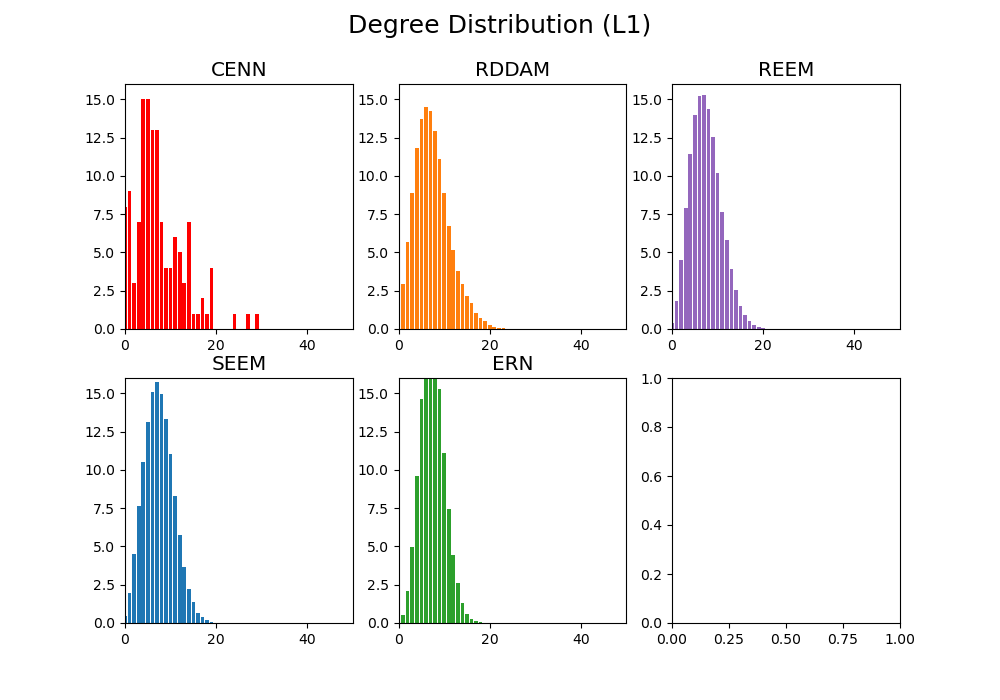
\includegraphics[width=0.32\linewidth]{../data/images/distributions/degreeDist_W1_Rand.png}
%     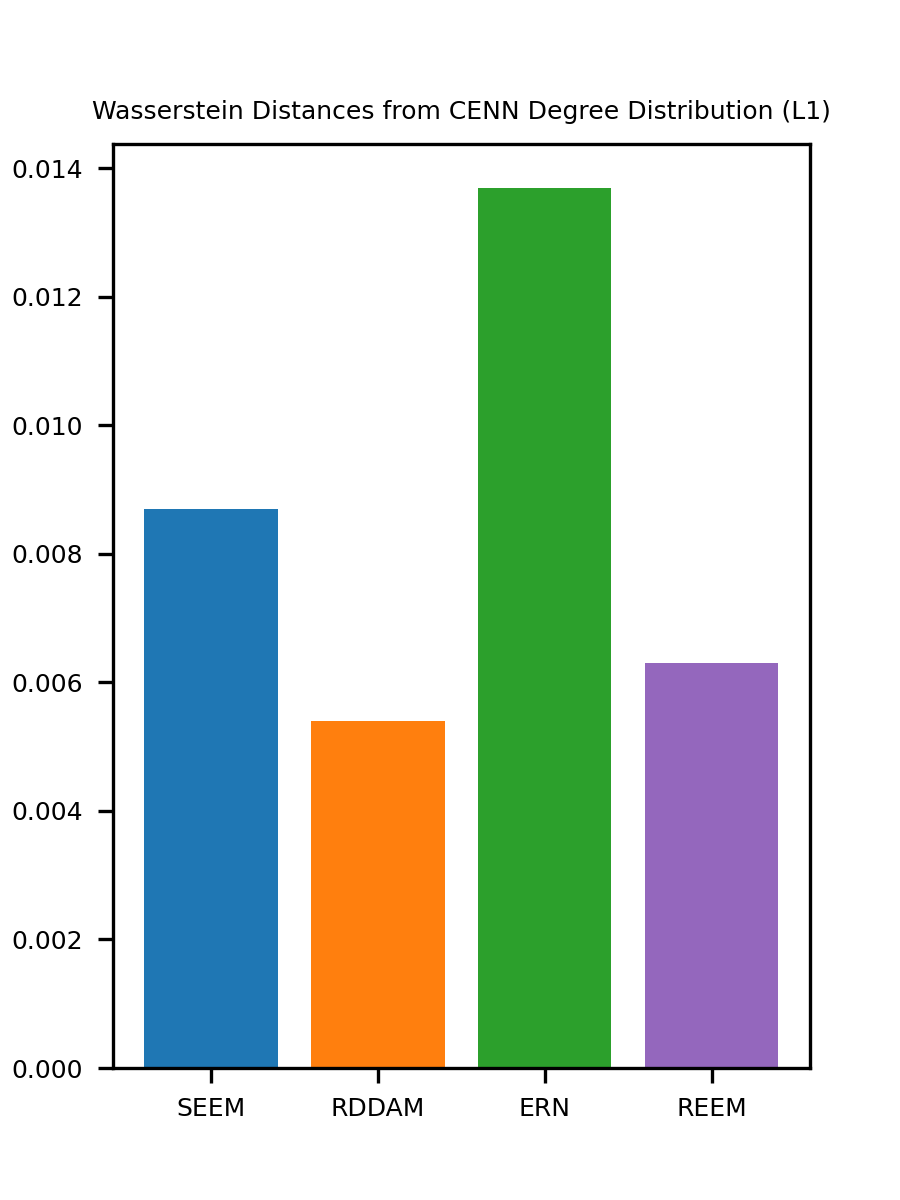
\includegraphics[width=0.17\linewidth]{../data/images/compareDistributions/wassersteinDistances_Degree_L1_3.png}
%     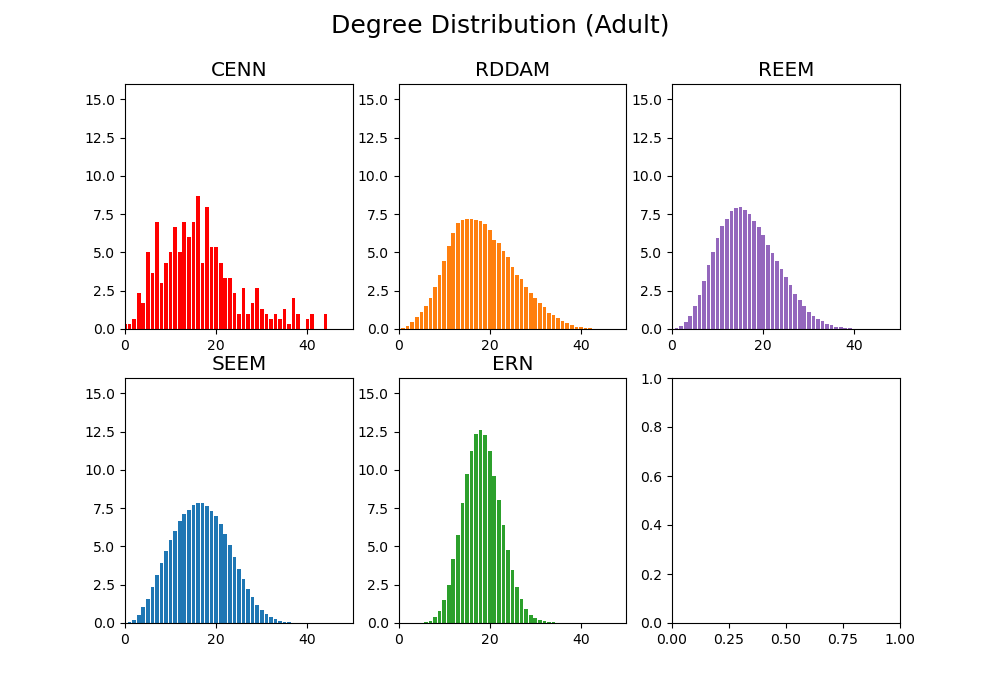
\includegraphics[width=0.32\linewidth]{../data/images/distributions/degreeDist_L5_Rand.png}
%     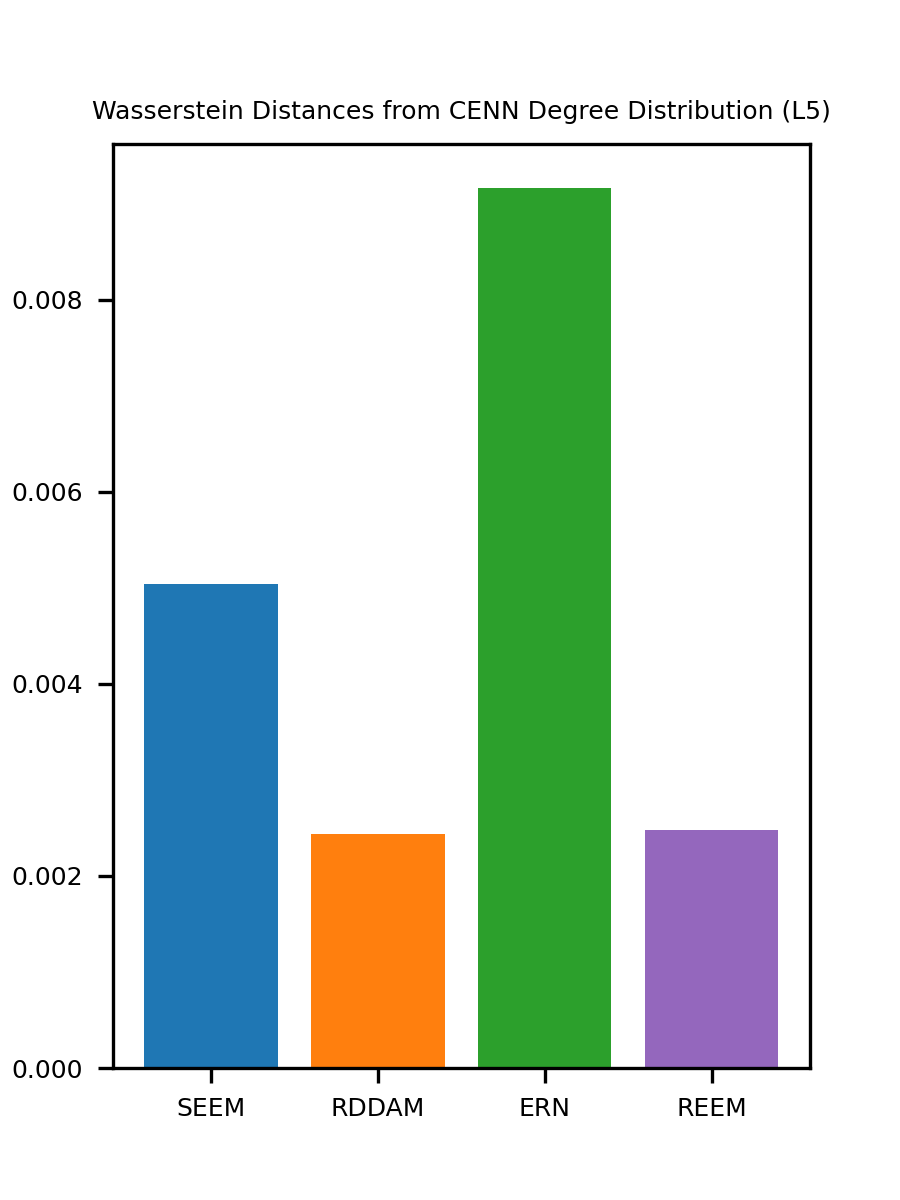
\includegraphics[width=0.17\linewidth]{../data/images/compareDistributions/wassersteinDistances_Degree_L5_3.png}

%     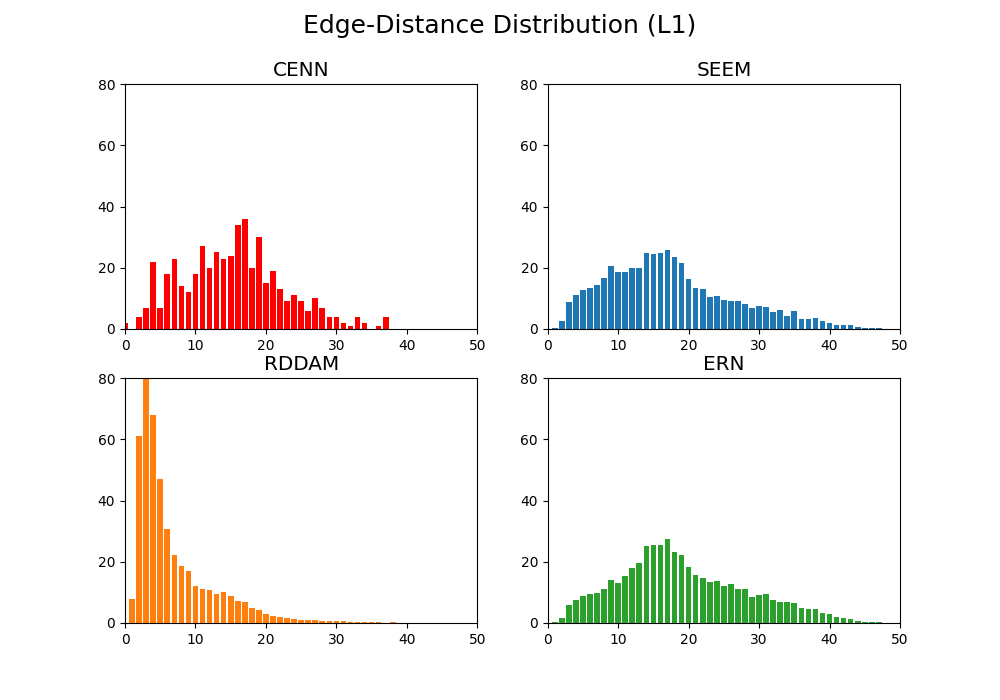
\includegraphics[width=0.32\linewidth]{../data/images/distributions/distDist_W1.png}
%     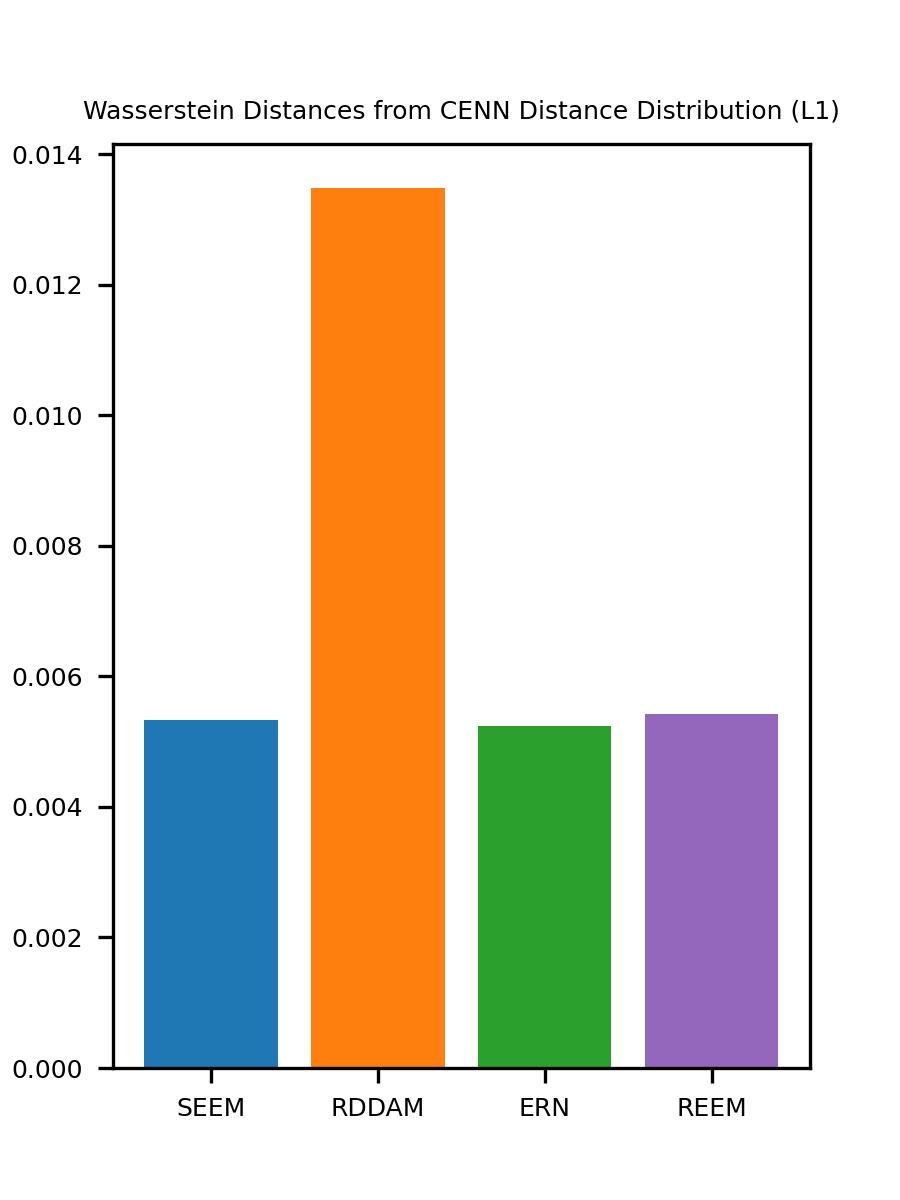
\includegraphics[width=0.17\linewidth]{../data/images/compareDistributions/wassersteinDistances_Distance_L1_3.png}
%     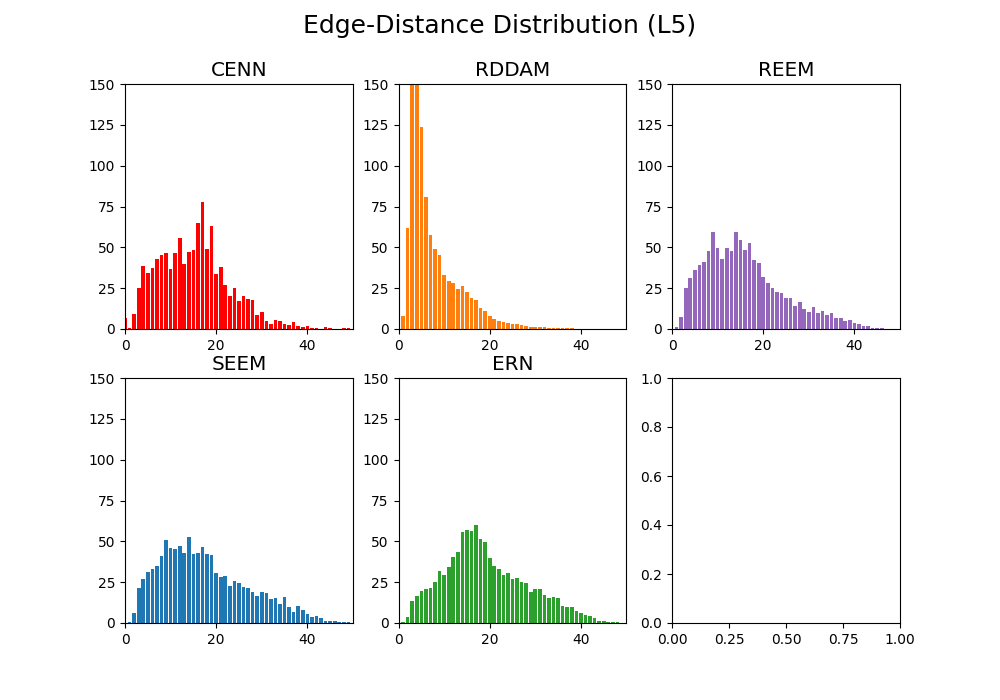
\includegraphics[width=0.32\linewidth]{../data/images/distributions/distDist_W8.png}
%     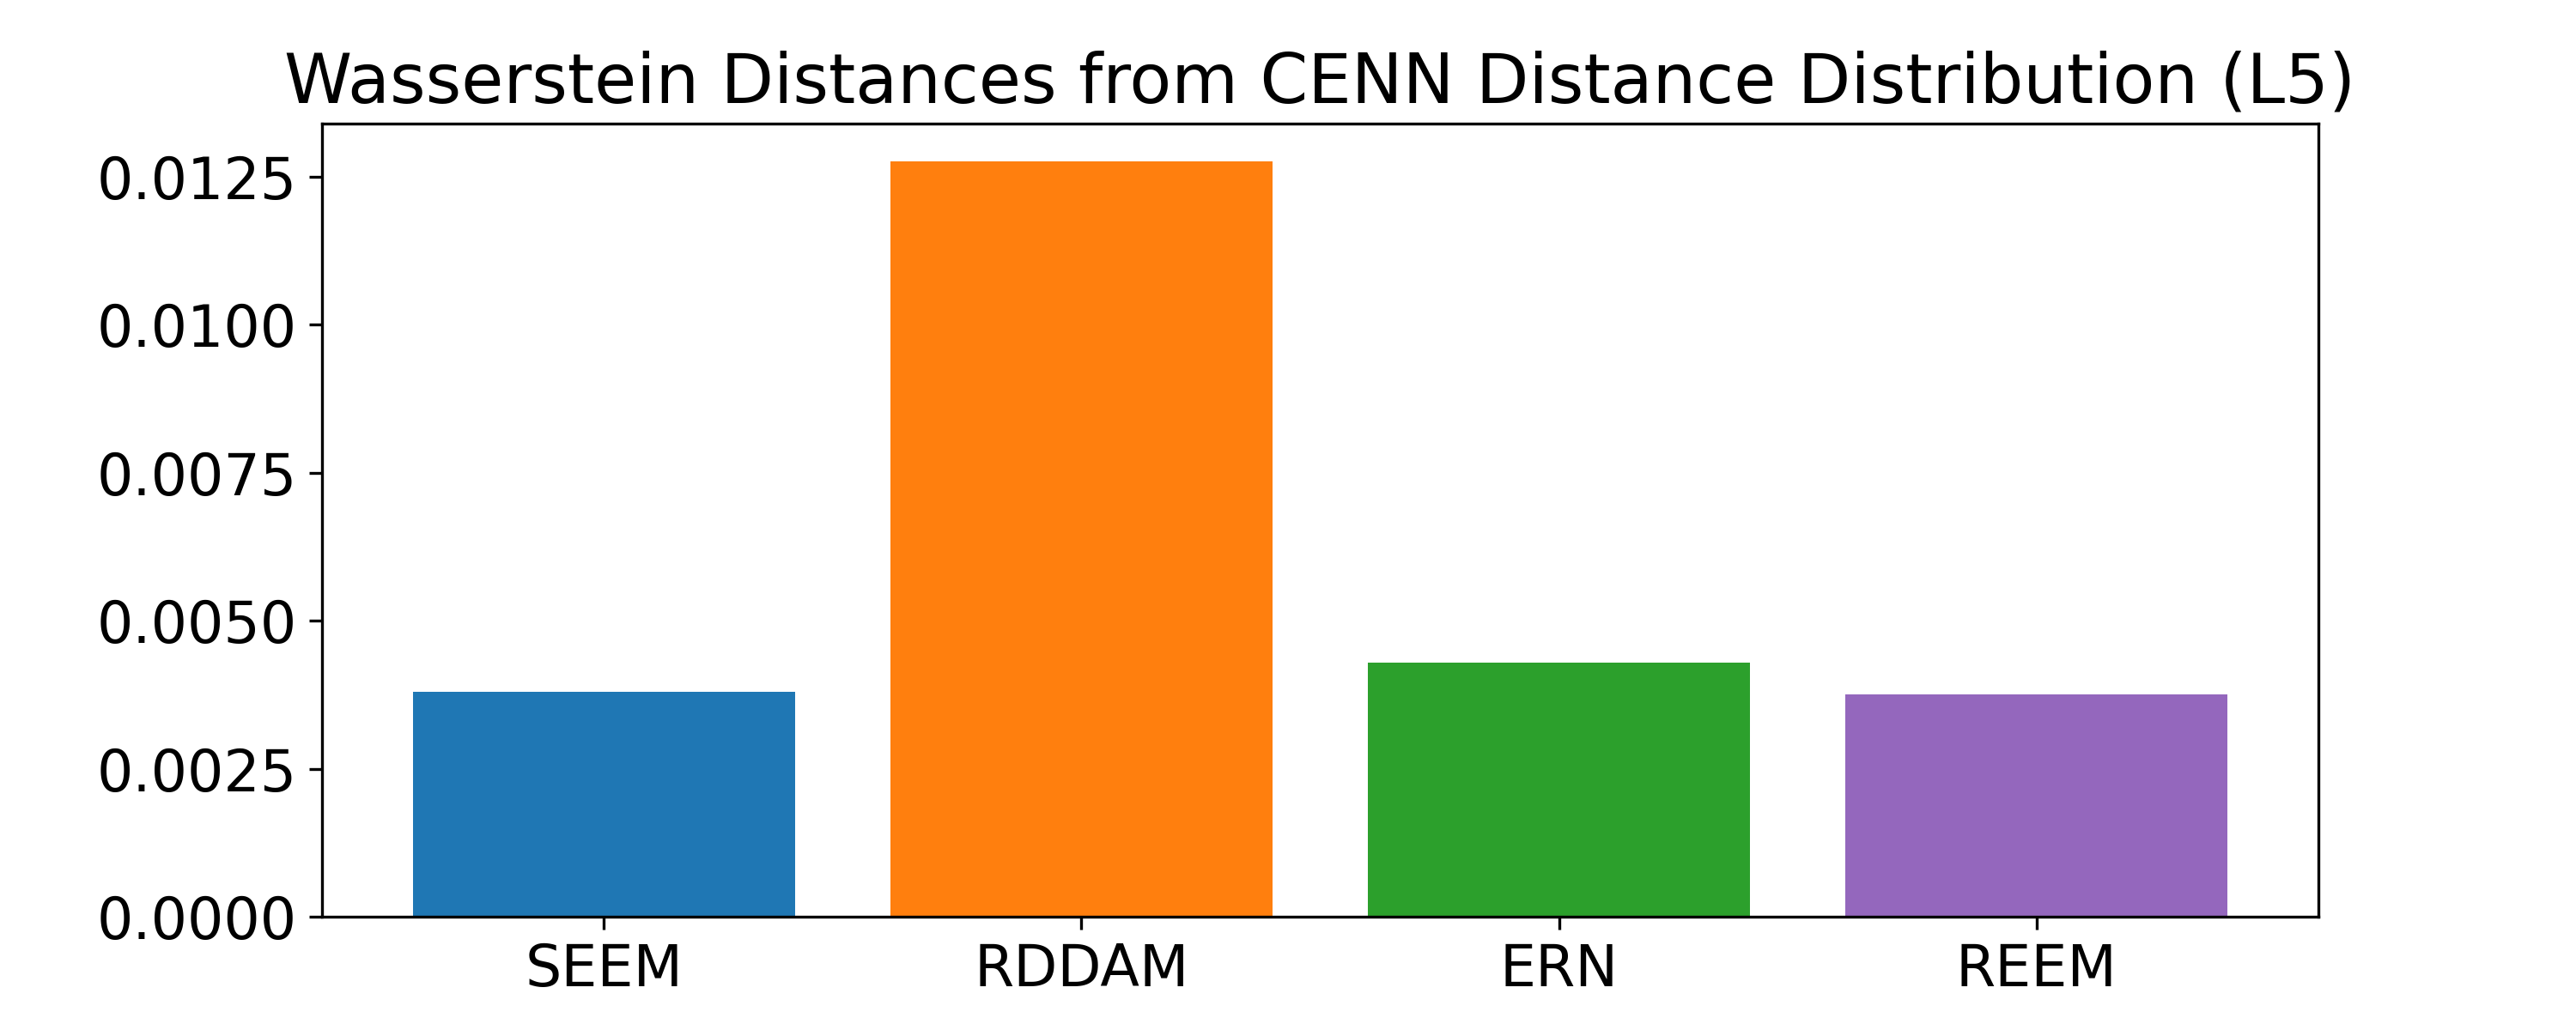
\includegraphics[width=0.17\linewidth]{../data/images/compareDistributions/wassersteinDistances_Distance_L5_3.png}

%     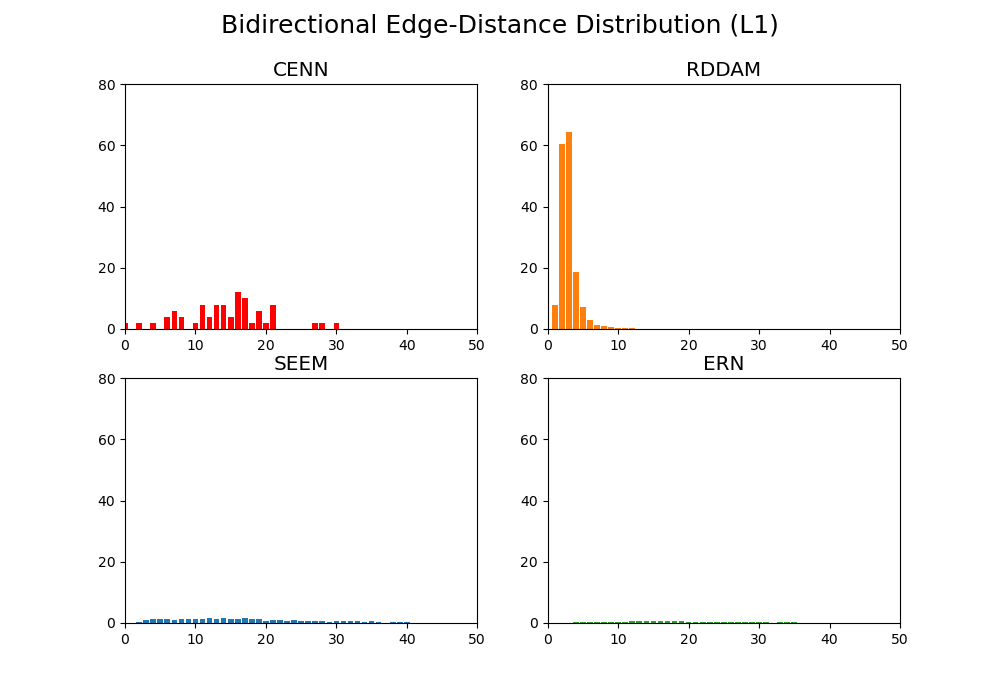
\includegraphics[width=0.32\linewidth]{../data/images/distributions/bidistDist_W1.png}
%     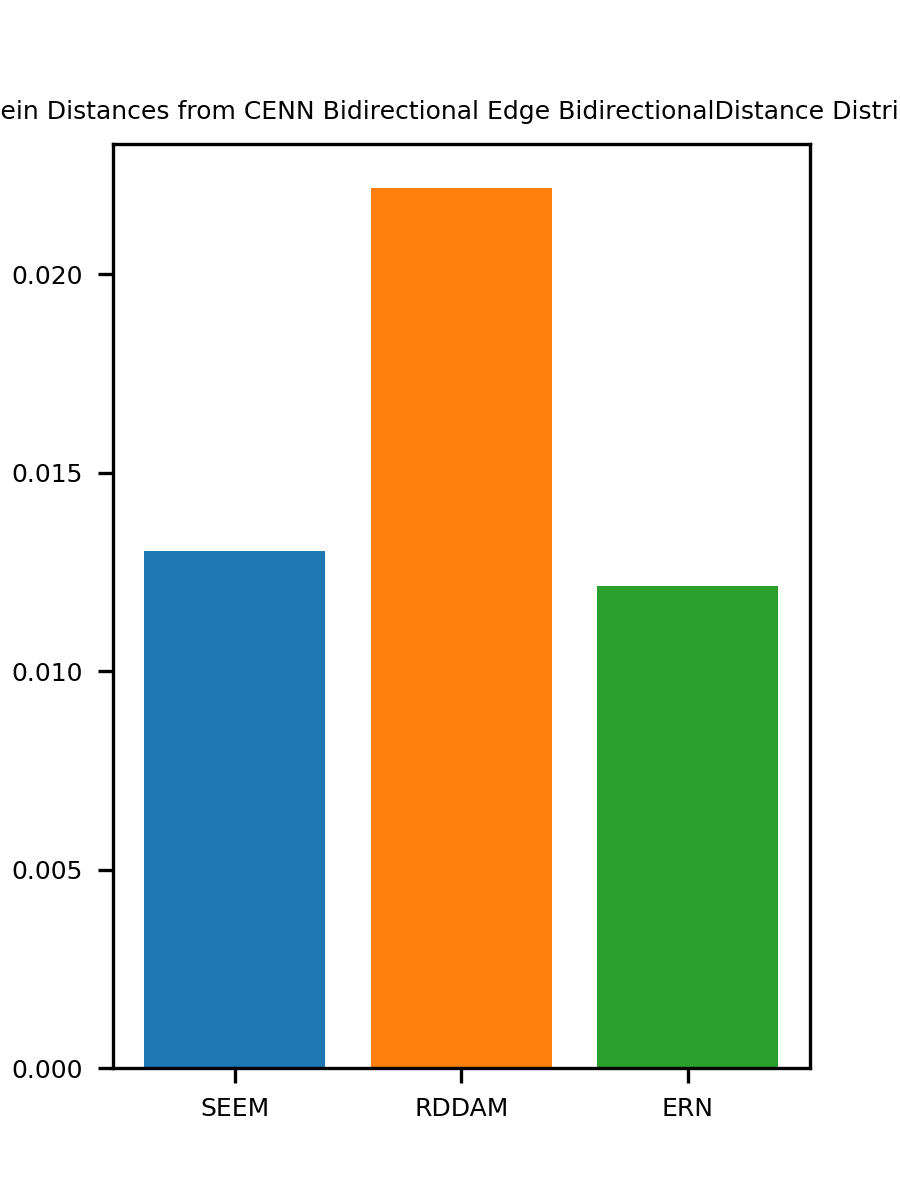
\includegraphics[width=0.17\linewidth]{../data/images/compareDistributions/wassersteinDistances_BidirectionalDistance_L1_3.png}
%     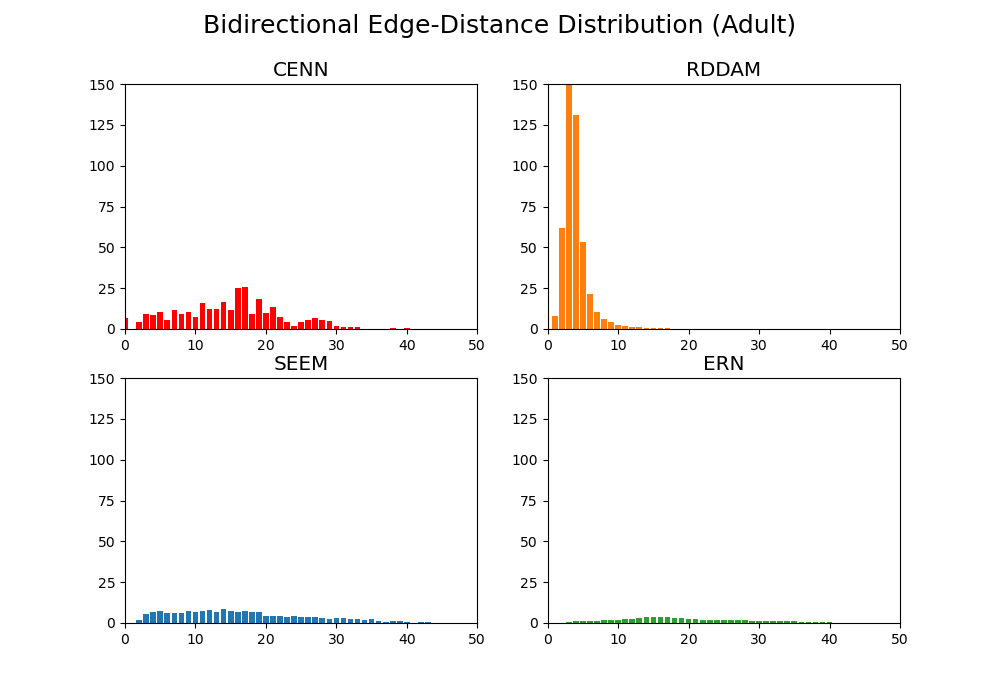
\includegraphics[width=0.32\linewidth]{../data/images/distributions/bidistDist_W8.png}
%     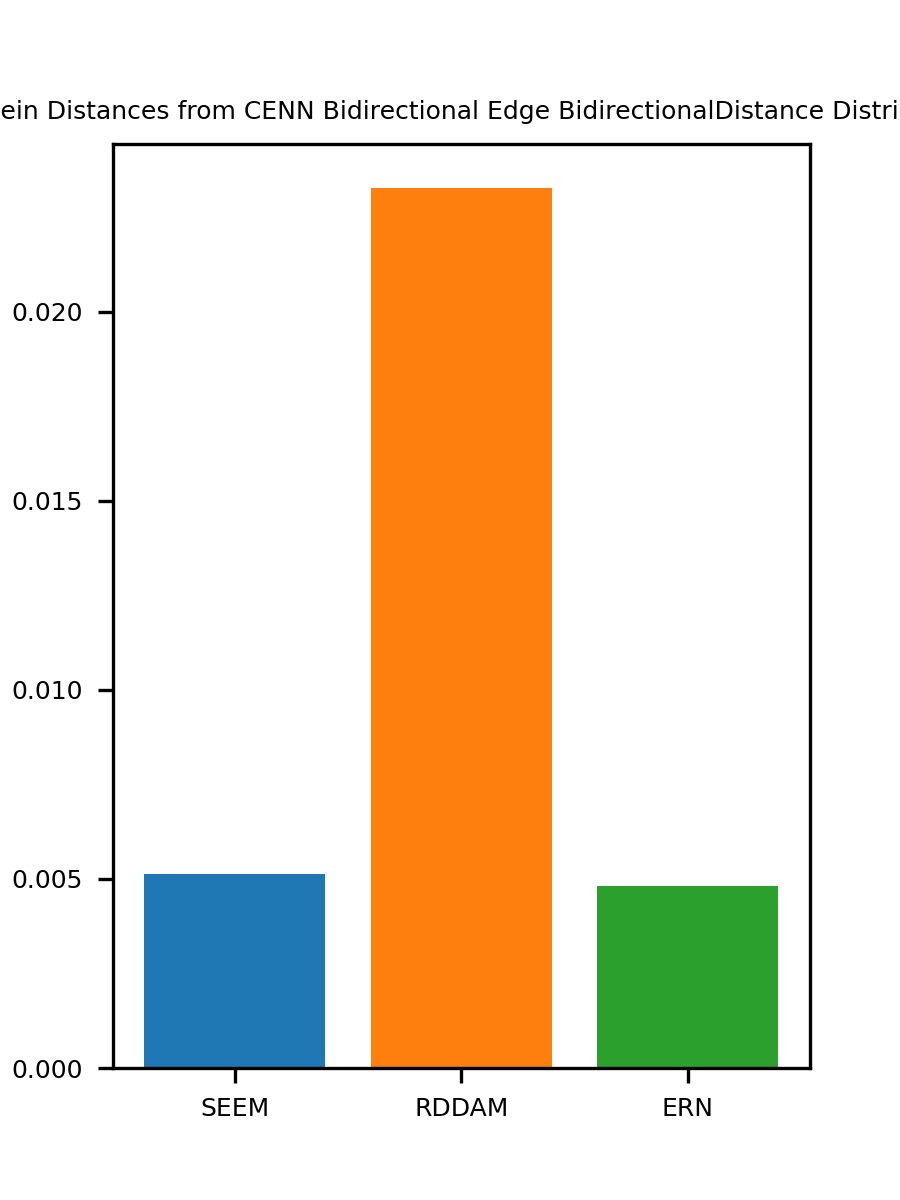
\includegraphics[width=0.17\linewidth]{../data/images/compareDistributions/wassersteinDistances_BidirectionalDistance_L5_3.png}

%   \caption{Degree distributions, plotting the number of nodes (y-axis) with a particular number of connections (x-axis). \textbf{NOTE:} Going to remove the purple sections from these graphs, use line graphs so I can overlap all distributions, add more caption, add letter labels, and will likely seperate and improve the bottom two graphs. }
% \end{figure}

\subsubsection{Distributions}

While these statistics give us an idea of how some of the attributes of these networks in describing the underlying structure of the CENN, it does not give us a picture of how the edges in any of these networks are distributed. We had two questions: 1) What is the structural makeup of these networks? (Are they scale-free, small-world, etc.?) 2) What is the physical makeup of these networks?

To answer these questions, we compared the degree distributions of these networks to examine their network structure and the distance distributions of these networks to examine their physical structure (see fig 2). To get a better idea of how similar these distributions were, we also measured their Wasserstein Distances from the \ce distribution. For the adults, these distributions were averaged.

\textit{Degree Distributions:} We found that our model and RDDAM to have degree distributions closest to \ce, with RDDAM being slightly closer. This is the first result which differentiates our model from random networks. These two models result in networks which appear to have more variability in degree than random networks. Since both rely on spatial proximity of nodes, which are not evenly distributed, it would be expected for their degree distributions to favor nodes which are closer to many others. This could explain why we see these results. It is notable that the degree distributions of CENN have much longer tales. This means that \ce connectomes are more centralized than any of the other networks being compared.

\textit{Distance Distributions:} The edge distances of each model show an issue with RDDAM: it favoring close connections. We see that our model is most like \ce in this distribution, the same as what we found when comparing average edge distributions. This indicates that \ce frontal ganglia is not particularly distance dependent as indicated in Itzhack \& Louzoun (2010). Given the similarity in the distributions, spatial embedding alone could explain for the edge distance distribution of \ce. 

\textit{Bidirectional Edges:} Given the results of comparing numbers of bidirectional edges in these networks, we were curious as to what these bidirectional connections looked like in \ce. Did they result from a preference for short connections, were they random, or were they distributed in a completely different way from any of our models. To answer this, we compared the edge distance distributions of all bidirectional edges in each graph (see fig 2). From the results, the bidirectionality of \ce frontal ganglia appears to be mostly random with the random graphs being closest to \ce and our model being a close second. RDDAM, preferring short connections, resulting in a very different looking distribution. Despite the number of bidirectional edges being between the amount shown in RDDAM and our model, it appears that these connections are random with respect to spatial distance. It is important to note that the number of bidirectional edges is still much higher than one would expect in a random graph. 

% \textbf{NOTE:} I need to reexamine the source data to understand if these connections are electric or chemical. Shouldn't we expect the majority of connections to be bidirectional since most are electrical? Is there a misinterepretation of the data?

\begin{figure*}[h]
  \includegraphics[width=\linewidth]{../data/images/other/SpatialOverlaps.png}
  \caption{INSERT HERE}
\end{figure*}

\subsubsection{Spatial Embedding}
\subsubsection{Overlaps}

\subsection{Breaking Down the Model}
What aspects of SEEM lead to a model that in some ways is more similar to the CENN? This model's input parameters are the location of the neurons, the expected number of connections, the location of the Nerve Ring (VALUE), and Epsilon (the maximum distance two neurites must have to form a potential connection. The first two of these parameters come from empirical data so they will not be adjusted. Adjustment of the location of the Nerve Ring cannot be meaningfully adjusted as there are only a small number of neurons which closely lie on this border, making such changes insignificantly impactful to the overall shape of the network. Rather than adjusting the nerve ring location, adjusting the algorithm for determining neurite direction may prove as more useful in parsing out the model's relavent parameters. 

\textbf{THIS IS WHERE WE TALK ABOUT THE RANDOM DIRECTION VERSION OF SEEM.}

% \subsection{Neurite Direction}
% Is neurite direction a significant factor in forming models which are similar to the CENN?

% \subsection{Attachment Distance}
% Is the maximum attachment distance between neurites important for creating a network more similar to the CENN?

% \section{OLD}
% \subsection{Network Statistics CHANGE}
% SEEM was found to be the set of networks closest to the CENN in average edge distance (see table 1 and fig 1). [INSERT STATS FOR STATISTICAL SIGNIFICANCE BETWEEN DISTRIBUTIONS]. RDDAM were closest to the CENN in average clustering coefficient and number of bidirectional links. [INSERT STATS FOR STATISTICAL SIGNIFICANCE BETWEEN DISTRIBUTIONS]. These results were not heavily dependent on which network was chosen.

% The degree distributions of RDDAM were also found to be most similar to the CENN with a Wasserstein Distance of 0.005 in L1 and 0.002 in adults (see fig 2). SEEM was close with a Wasserstein Distance of 0.006 in L1 and 0.003 in adults, making the distinction between the two insignificant. The degree distributions of Erdos-Renyi graphs appeared much less like the CENN with a Wasserstein Distance of 0.013 in L1 and 0.009 in adults. The average degree between all four graphs were not significantly different.




% Comparing the distribution of edge distances shows a different picture. Here, the resulting graphs of SEEM were found to be closest to the CENN (see fig 3). The edge distance distributions in SEEM had a Wasserstein Distance of 0.004 in L1 and 0.003 in adults. The Erdos-Renyi graphs, with a Wasserstein Distance of 0.005 in L1 and 0.004 in adults, were even more similar to CENN than the RDDAM, with a Wasserstein Distance of 0.013 in L1 and adults. These results distinguish SEEM from RDDAM, showing the proclivity of RDDAM to form very short connections, something SEEM does not appear to do.

% Spatially embedding these graphs using provided coordinates resulted in a particular connectivity pattern shared between the CENN and SEEM graphs (see Figure 4). [INSERT DATA ABOUT DISTRIBUTION OF CROSS-PHARYNX CONNECTIONS]